\documentclass[twoside]{book}

% Packages required by doxygen
\usepackage{fixltx2e}
\usepackage{calc}
\usepackage{doxygen}
\usepackage[export]{adjustbox} % also loads graphicx
\usepackage{graphicx}
\usepackage[utf8]{inputenc}
\usepackage{makeidx}
\usepackage{multicol}
\usepackage{multirow}
\PassOptionsToPackage{warn}{textcomp}
\usepackage{textcomp}
\usepackage[nointegrals]{wasysym}
\usepackage[table]{xcolor}

% Font selection
\usepackage[T1]{fontenc}
\usepackage[scaled=.90]{helvet}
\usepackage{courier}
\usepackage{amssymb}
\usepackage{sectsty}
\renewcommand{\familydefault}{\sfdefault}
\allsectionsfont{%
  \fontseries{bc}\selectfont%
  \color{darkgray}%
}
\renewcommand{\DoxyLabelFont}{%
  \fontseries{bc}\selectfont%
  \color{darkgray}%
}
\newcommand{\+}{\discretionary{\mbox{\scriptsize$\hookleftarrow$}}{}{}}

% Page & text layout
\usepackage{geometry}
\geometry{%
  a4paper,%
  top=2.5cm,%
  bottom=2.5cm,%
  left=2.5cm,%
  right=2.5cm%
}
\tolerance=750
\hfuzz=15pt
\hbadness=750
\setlength{\emergencystretch}{15pt}
\setlength{\parindent}{0cm}
\setlength{\parskip}{0.2cm}
\makeatletter
\renewcommand{\paragraph}{%
  \@startsection{paragraph}{4}{0ex}{-1.0ex}{1.0ex}{%
    \normalfont\normalsize\bfseries\SS@parafont%
  }%
}
\renewcommand{\subparagraph}{%
  \@startsection{subparagraph}{5}{0ex}{-1.0ex}{1.0ex}{%
    \normalfont\normalsize\bfseries\SS@subparafont%
  }%
}
\makeatother

% Headers & footers
\usepackage{fancyhdr}
\pagestyle{fancyplain}
\fancyhead[LE]{\fancyplain{}{\bfseries\thepage}}
\fancyhead[CE]{\fancyplain{}{}}
\fancyhead[RE]{\fancyplain{}{\bfseries\leftmark}}
\fancyhead[LO]{\fancyplain{}{\bfseries\rightmark}}
\fancyhead[CO]{\fancyplain{}{}}
\fancyhead[RO]{\fancyplain{}{\bfseries\thepage}}
\fancyfoot[LE]{\fancyplain{}{}}
\fancyfoot[CE]{\fancyplain{}{}}
\fancyfoot[RE]{\fancyplain{}{\bfseries\scriptsize Generated on Thu Mar 3 2016 22\+:16\+:47 for Design by Doxygen }}
\fancyfoot[LO]{\fancyplain{}{\bfseries\scriptsize Generated on Thu Mar 3 2016 22\+:16\+:47 for Design by Doxygen }}
\fancyfoot[CO]{\fancyplain{}{}}
\fancyfoot[RO]{\fancyplain{}{}}
\renewcommand{\footrulewidth}{0.4pt}
\renewcommand{\chaptermark}[1]{%
  \markboth{#1}{}%
}
\renewcommand{\sectionmark}[1]{%
  \markright{\thesection\ #1}%
}

% Indices & bibliography
\usepackage{natbib}
\usepackage[titles]{tocloft}
\setcounter{tocdepth}{3}
\setcounter{secnumdepth}{5}
\makeindex

% Hyperlinks (required, but should be loaded last)
\usepackage{ifpdf}
\ifpdf
  \usepackage[pdftex,pagebackref=true]{hyperref}
\else
  \usepackage[ps2pdf,pagebackref=true]{hyperref}
\fi
\hypersetup{%
  colorlinks=true,%
  linkcolor=blue,%
  citecolor=blue,%
  unicode%
}

% Custom commands
\newcommand{\clearemptydoublepage}{%
  \newpage{\pagestyle{empty}\cleardoublepage}%
}


%===== C O N T E N T S =====

\begin{document}

% Titlepage & ToC
\hypersetup{pageanchor=false,
             bookmarks=true,
             bookmarksnumbered=true,
             pdfencoding=unicode
            }
\pagenumbering{roman}
\begin{titlepage}
\vspace*{7cm}
\begin{center}%
{\Large Design \\[1ex]\large 1.\+0 }\\
\vspace*{1cm}
{\large Generated by Doxygen 1.8.9.1}\\
\vspace*{0.5cm}
{\small Thu Mar 3 2016 22:16:47}\\
\end{center}
\end{titlepage}
%\clearemptydoublepage
\tableofcontents
%\clearemptydoublepage
\pagenumbering{arabic}
\hypersetup{pageanchor=true}

%--- Begin generated contents ---
%\chapter{Namespace Index}
%\section{Namespace List}
Here is a list of all namespaces with brief descriptions\+:\begin{DoxyCompactList}
\item\contentsline{section}{\hyperlink{namespaceel}{el} \\*Easylogging++ entry namespace }{\pageref{namespaceel}}{}
\item\contentsline{section}{\hyperlink{namespaceel_1_1base}{el\+::base} \\*Namespace containing base/internal functionality used by Easylogging++ }{\pageref{namespaceel_1_1base}}{}
\item\contentsline{section}{\hyperlink{namespaceel_1_1base_1_1consts}{el\+::base\+::consts} \\*Namespace containing constants used internally }{\pageref{namespaceel_1_1base_1_1consts}}{}
\item\contentsline{section}{\hyperlink{namespaceel_1_1base_1_1debug}{el\+::base\+::debug} \\*Contains some internal debugging tools like crash handler and stack tracer }{\pageref{namespaceel_1_1base_1_1debug}}{}
\item\contentsline{section}{\hyperlink{namespaceel_1_1base_1_1threading}{el\+::base\+::threading} }{\pageref{namespaceel_1_1base_1_1threading}}{}
\item\contentsline{section}{\hyperlink{namespaceel_1_1base_1_1threading_1_1internal}{el\+::base\+::threading\+::internal} }{\pageref{namespaceel_1_1base_1_1threading_1_1internal}}{}
\item\contentsline{section}{\hyperlink{namespaceel_1_1base_1_1type}{el\+::base\+::type} \\*Data types used by Easylogging++ }{\pageref{namespaceel_1_1base_1_1type}}{}
\item\contentsline{section}{\hyperlink{namespaceel_1_1base_1_1utils}{el\+::base\+::utils} \\*Namespace containing utility functions/static classes used internally }{\pageref{namespaceel_1_1base_1_1utils}}{}
\item\contentsline{section}{\hyperlink{namespaceel_1_1base_1_1utils_1_1bitwise}{el\+::base\+::utils\+::bitwise} \\*Bitwise operations for C++11 strong enum class. This casts e into Flag\+\_\+\+T and returns value after bitwise operation Use these function as }{\pageref{namespaceel_1_1base_1_1utils_1_1bitwise}}{}
\end{DoxyCompactList}

\chapter{Hierarchical Index}
\section{Class Hierarchy}
This inheritance list is sorted roughly, but not completely, alphabetically\+:\begin{DoxyCompactList}
\item \contentsline{section}{\+\_\+\+Statistic\+Inquiry}{\pageref{struct___statistic_inquiry}}{}
\item \contentsline{section}{\+\_\+\+Task}{\pageref{struct___task}}{}
\item \contentsline{section}{\+\_\+\+Task\+Data}{\pageref{struct___task_data}}{}
\item \contentsline{section}{el\+:\+:base\+:\+:utils\+:\+:Command\+Line\+Args}{\pageref{classel_1_1base_1_1utils_1_1_command_line_args}}{}
\item \contentsline{section}{Command\+Line\+Parser}{\pageref{class_command_line_parser}}{}
\item \contentsline{section}{Comparison\+Class\+L\+J\+F}{\pageref{class_comparison_class_l_j_f}}{}
\item \contentsline{section}{Comparison\+Class\+S\+J\+F}{\pageref{class_comparison_class_s_j_f}}{}
\item \contentsline{section}{el\+:\+:Custom\+Format\+Specifier}{\pageref{classel_1_1_custom_format_specifier}}{}
\item \contentsline{section}{Database}{\pageref{class_database}}{}
\begin{DoxyCompactList}
\item \contentsline{section}{Bookkeeping\+Database}{\pageref{class_bookkeeping_database}}{}
\item \contentsline{section}{Statistic\+Database}{\pageref{class_statistic_database}}{}
\end{DoxyCompactList}
\item \contentsline{section}{Database\+Handler}{\pageref{class_database_handler}}{}
\item \contentsline{section}{Data\+Mining}{\pageref{class_data_mining}}{}
\begin{DoxyCompactList}
\item \contentsline{section}{Dummy\+Data\+Mining}{\pageref{class_dummy_data_mining}}{}
\item \contentsline{section}{Grid\+Data\+Mining}{\pageref{class_grid_data_mining}}{}
\end{DoxyCompactList}
\item \contentsline{section}{Executor}{\pageref{class_executor}}{}
\begin{DoxyCompactList}
\item \contentsline{section}{Abstract\+Scheduler}{\pageref{class_abstract_scheduler}}{}
\begin{DoxyCompactList}
\item \contentsline{section}{Master}{\pageref{class_master}}{}
\item \contentsline{section}{Task\+Stealing\+Scheduler}{\pageref{class_task_stealing_scheduler}}{}
\end{DoxyCompactList}
\item \contentsline{section}{Database\+Server}{\pageref{class_database_server}}{}
\item \contentsline{section}{Worker\+Executor}{\pageref{class_worker_executor}}{}
\end{DoxyCompactList}
\item \contentsline{section}{Grid\+Creator}{\pageref{class_grid_creator}}{}
\item \contentsline{section}{Grid\+Predictor}{\pageref{class_grid_predictor}}{}
\item \contentsline{section}{el\+:\+:base\+:\+:Hit\+Counter}{\pageref{classel_1_1base_1_1_hit_counter}}{}
\item \contentsline{section}{el\+:\+:Log\+Dispatch\+Data}{\pageref{classel_1_1_log_dispatch_data}}{}
\item \contentsline{section}{el\+:\+:Loggable}{\pageref{classel_1_1_loggable}}{}
\begin{DoxyCompactList}
\item \contentsline{section}{el\+:\+:base\+:\+:Log\+Format}{\pageref{classel_1_1base_1_1_log_format}}{}
\item \contentsline{section}{el\+:\+:base\+:\+:Performance\+Tracker}{\pageref{classel_1_1base_1_1_performance_tracker}}{}
\item \contentsline{section}{el\+:\+:Configuration}{\pageref{classel_1_1_configuration}}{}
\item \contentsline{section}{el\+:\+:Logger}{\pageref{classel_1_1_logger}}{}
\end{DoxyCompactList}
\item \contentsline{section}{el\+:\+:Log\+Message}{\pageref{classel_1_1_log_message}}{}
\item \contentsline{section}{el\+:\+:base\+:\+:Message\+Builder}{\pageref{classel_1_1base_1_1_message_builder}}{}
\item \contentsline{section}{el\+:\+:base\+:\+:Milliseconds\+Width}{\pageref{classel_1_1base_1_1_milliseconds_width}}{}
\item \contentsline{section}{el\+:\+:base\+:\+:No\+Copy}{\pageref{classel_1_1base_1_1_no_copy}}{}
\begin{DoxyCompactList}
\item \contentsline{section}{el\+:\+:base\+:\+:debug\+:\+:Crash\+Handler}{\pageref{classel_1_1base_1_1debug_1_1_crash_handler}}{}
\item \contentsline{section}{el\+:\+:base\+:\+:debug\+:\+:Stack\+Trace}{\pageref{classel_1_1base_1_1debug_1_1_stack_trace}}{}
\item \contentsline{section}{el\+:\+:base\+:\+:Log\+Dispatcher}{\pageref{classel_1_1base_1_1_log_dispatcher}}{}
\item \contentsline{section}{el\+:\+:base\+:\+:Null\+Writer}{\pageref{classel_1_1base_1_1_null_writer}}{}
\item \contentsline{section}{el\+:\+:base\+:\+:Storage}{\pageref{classel_1_1base_1_1_storage}}{}
\item \contentsline{section}{el\+:\+:base\+:\+:threading\+:\+:internal\+:\+:No\+Mutex}{\pageref{classel_1_1base_1_1threading_1_1internal_1_1_no_mutex}}{}
\item \contentsline{section}{el\+:\+:base\+:\+:threading\+:\+:internal\+:\+:No\+Scoped\+Lock$<$ Mutex $>$}{\pageref{classel_1_1base_1_1threading_1_1internal_1_1_no_scoped_lock}}{}
\item \contentsline{section}{el\+:\+:base\+:\+:V\+Registry}{\pageref{classel_1_1base_1_1_v_registry}}{}
\item \contentsline{section}{el\+:\+:base\+:\+:Writer}{\pageref{classel_1_1base_1_1_writer}}{}
\begin{DoxyCompactList}
\item \contentsline{section}{el\+:\+:base\+:\+:P\+Error\+Writer}{\pageref{classel_1_1base_1_1_p_error_writer}}{}
\end{DoxyCompactList}
\item \contentsline{section}{el\+:\+:Log\+Builder}{\pageref{classel_1_1_log_builder}}{}
\begin{DoxyCompactList}
\item \contentsline{section}{el\+:\+:base\+:\+:Default\+Log\+Builder}{\pageref{classel_1_1base_1_1_default_log_builder}}{}
\end{DoxyCompactList}
\end{DoxyCompactList}
\item \contentsline{section}{el\+:\+:Performance\+Tracking\+Data}{\pageref{classel_1_1_performance_tracking_data}}{}
\item \contentsline{section}{el\+:\+:Configuration\+:\+:Predicate}{\pageref{classel_1_1_configuration_1_1_predicate}}{}
\item \contentsline{section}{el\+:\+:base\+:\+:Hit\+Counter\+:\+:Predicate}{\pageref{classel_1_1base_1_1_hit_counter_1_1_predicate}}{}
\item \contentsline{section}{Scheduler\+Test\+Suite}{\pageref{class_scheduler_test_suite}}{}
\item \contentsline{section}{Scheduling\+Strategy}{\pageref{class_scheduling_strategy}}{}
\begin{DoxyCompactList}
\item \contentsline{section}{F\+I\+F\+O}{\pageref{class_f_i_f_o}}{}
\item \contentsline{section}{L\+I\+F\+O}{\pageref{class_l_i_f_o}}{}
\item \contentsline{section}{L\+J\+F}{\pageref{class_l_j_f}}{}
\item \contentsline{section}{Mpi\+Win\+Scheduling\+Strategy}{\pageref{class_mpi_win_scheduling_strategy}}{}
\begin{DoxyCompactList}
\item \contentsline{section}{Mpi\+Win\+F\+I\+F\+O}{\pageref{class_mpi_win_f_i_f_o}}{}
\item \contentsline{section}{Mpi\+Win\+L\+I\+F\+O}{\pageref{class_mpi_win_l_i_f_o}}{}
\end{DoxyCompactList}
\item \contentsline{section}{S\+J\+F}{\pageref{class_s_j_f}}{}
\end{DoxyCompactList}
\item \contentsline{section}{Scheduling\+Strategy\+Evaluator}{\pageref{class_scheduling_strategy_evaluator}}{}
\item \contentsline{section}{el\+:\+:Loggers\+:\+:Scoped\+Add\+Flag}{\pageref{classel_1_1_loggers_1_1_scoped_add_flag}}{}
\item \contentsline{section}{el\+:\+:Loggers\+:\+:Scoped\+Remove\+Flag}{\pageref{classel_1_1_loggers_1_1_scoped_remove_flag}}{}
\item \contentsline{section}{el\+:\+:base\+:\+:debug\+:\+:Stack\+Trace\+:\+:Stack\+Trace\+Entry}{\pageref{classel_1_1base_1_1debug_1_1_stack_trace_1_1_stack_trace_entry}}{}
\item \contentsline{section}{el\+:\+:base\+:\+:Static\+Class}{\pageref{classel_1_1base_1_1_static_class}}{}
\begin{DoxyCompactList}
\item \contentsline{section}{el\+:\+:base\+:\+:utils\+:\+:Date\+Time}{\pageref{classel_1_1base_1_1utils_1_1_date_time}}{}
\item \contentsline{section}{el\+:\+:base\+:\+:utils\+:\+:File}{\pageref{classel_1_1base_1_1utils_1_1_file}}{}
\item \contentsline{section}{el\+:\+:base\+:\+:utils\+:\+:O\+S}{\pageref{classel_1_1base_1_1utils_1_1_o_s}}{}
\item \contentsline{section}{el\+:\+:base\+:\+:utils\+:\+:Str}{\pageref{classel_1_1base_1_1utils_1_1_str}}{}
\item \contentsline{section}{el\+:\+:Configurations\+:\+:Parser}{\pageref{classel_1_1_configurations_1_1_parser}}{}
\item \contentsline{section}{el\+:\+:Configuration\+Type\+Helper}{\pageref{classel_1_1_configuration_type_helper}}{}
\item \contentsline{section}{el\+:\+:Helpers}{\pageref{classel_1_1_helpers}}{}
\item \contentsline{section}{el\+:\+:Level\+Helper}{\pageref{classel_1_1_level_helper}}{}
\item \contentsline{section}{el\+:\+:Loggers}{\pageref{classel_1_1_loggers}}{}
\item \contentsline{section}{el\+:\+:Version\+Info}{\pageref{classel_1_1_version_info}}{}
\end{DoxyCompactList}
\item \contentsline{section}{el\+:\+:Sys\+Log\+Initializer}{\pageref{classel_1_1_sys_log_initializer}}{}
\item Test\+Fixture\begin{DoxyCompactList}
\item \contentsline{section}{F\+I\+F\+O\+Test\+Case}{\pageref{class_f_i_f_o_test_case}}{}
\item \contentsline{section}{L\+I\+F\+O\+Test\+Case}{\pageref{class_l_i_f_o_test_case}}{}
\item \contentsline{section}{L\+J\+F\+Test\+Case}{\pageref{class_l_j_f_test_case}}{}
\item \contentsline{section}{S\+J\+F\+Test\+Case}{\pageref{class_s_j_f_test_case}}{}
\end{DoxyCompactList}
\item \contentsline{section}{el\+:\+:base\+:\+:threading\+:\+:Thread\+Safe}{\pageref{classel_1_1base_1_1threading_1_1_thread_safe}}{}
\begin{DoxyCompactList}
\item \contentsline{section}{el\+:\+:base\+:\+:utils\+:\+:Abstract\+Registry$<$ base\+:\+:Hit\+Counter, std\+:\+:vector$<$ base\+:\+:Hit\+Counter $\ast$ $>$ $>$}{\pageref{classel_1_1base_1_1utils_1_1_abstract_registry}}{}
\begin{DoxyCompactList}
\item \contentsline{section}{el\+:\+:base\+:\+:utils\+:\+:Registry\+With\+Pred$<$ base\+:\+:Hit\+Counter, base\+:\+:Hit\+Counter\+:\+:Predicate $>$}{\pageref{classel_1_1base_1_1utils_1_1_registry_with_pred}}{}
\begin{DoxyCompactList}
\item \contentsline{section}{el\+:\+:base\+:\+:Registered\+Hit\+Counters}{\pageref{classel_1_1base_1_1_registered_hit_counters}}{}
\end{DoxyCompactList}
\end{DoxyCompactList}
\item \contentsline{section}{el\+:\+:base\+:\+:utils\+:\+:Abstract\+Registry$<$ Configuration, std\+:\+:vector$<$ Configuration $\ast$ $>$ $>$}{\pageref{classel_1_1base_1_1utils_1_1_abstract_registry}}{}
\begin{DoxyCompactList}
\item \contentsline{section}{el\+:\+:base\+:\+:utils\+:\+:Registry\+With\+Pred$<$ Configuration, Configuration\+:\+:Predicate $>$}{\pageref{classel_1_1base_1_1utils_1_1_registry_with_pred}}{}
\begin{DoxyCompactList}
\item \contentsline{section}{el\+:\+:Configurations}{\pageref{classel_1_1_configurations}}{}
\end{DoxyCompactList}
\end{DoxyCompactList}
\item \contentsline{section}{el\+:\+:base\+:\+:utils\+:\+:Abstract\+Registry$<$ Logger, std\+:\+:map$<$ std\+:\+:string, Logger $\ast$ $>$ $>$}{\pageref{classel_1_1base_1_1utils_1_1_abstract_registry}}{}
\begin{DoxyCompactList}
\item \contentsline{section}{el\+:\+:base\+:\+:utils\+:\+:Registry$<$ Logger, std\+:\+:string $>$}{\pageref{classel_1_1base_1_1utils_1_1_registry}}{}
\begin{DoxyCompactList}
\item \contentsline{section}{el\+:\+:base\+:\+:Registered\+Loggers}{\pageref{classel_1_1base_1_1_registered_loggers}}{}
\end{DoxyCompactList}
\end{DoxyCompactList}
\item \contentsline{section}{el\+:\+:base\+:\+:utils\+:\+:Abstract\+Registry$<$ T\+\_\+\+Ptr, std\+:\+:map$<$ T\+\_\+\+Key, T\+\_\+\+Ptr $\ast$ $>$ $>$}{\pageref{classel_1_1base_1_1utils_1_1_abstract_registry}}{}
\begin{DoxyCompactList}
\item \contentsline{section}{el\+:\+:base\+:\+:utils\+:\+:Registry$<$ T\+\_\+\+Ptr, T\+\_\+\+Key $>$}{\pageref{classel_1_1base_1_1utils_1_1_registry}}{}
\end{DoxyCompactList}
\item \contentsline{section}{el\+:\+:base\+:\+:utils\+:\+:Abstract\+Registry$<$ T\+\_\+\+Ptr, std\+:\+:vector$<$ T\+\_\+\+Ptr $\ast$ $>$ $>$}{\pageref{classel_1_1base_1_1utils_1_1_abstract_registry}}{}
\begin{DoxyCompactList}
\item \contentsline{section}{el\+:\+:base\+:\+:utils\+:\+:Registry\+With\+Pred$<$ T\+\_\+\+Ptr, Pred $>$}{\pageref{classel_1_1base_1_1utils_1_1_registry_with_pred}}{}
\end{DoxyCompactList}
\item \contentsline{section}{el\+:\+:Callback$<$ Log\+Dispatch\+Data $>$}{\pageref{classel_1_1_callback}}{}
\begin{DoxyCompactList}
\item \contentsline{section}{el\+:\+:Log\+Dispatch\+Callback}{\pageref{classel_1_1_log_dispatch_callback}}{}
\begin{DoxyCompactList}
\item \contentsline{section}{el\+:\+:base\+:\+:Default\+Log\+Dispatch\+Callback}{\pageref{classel_1_1base_1_1_default_log_dispatch_callback}}{}
\end{DoxyCompactList}
\end{DoxyCompactList}
\item \contentsline{section}{el\+:\+:Callback$<$ Performance\+Tracking\+Data $>$}{\pageref{classel_1_1_callback}}{}
\begin{DoxyCompactList}
\item \contentsline{section}{el\+:\+:Performance\+Tracking\+Callback}{\pageref{classel_1_1_performance_tracking_callback}}{}
\begin{DoxyCompactList}
\item \contentsline{section}{el\+:\+:base\+:\+:Default\+Performance\+Tracking\+Callback}{\pageref{classel_1_1base_1_1_default_performance_tracking_callback}}{}
\end{DoxyCompactList}
\end{DoxyCompactList}
\item \contentsline{section}{el\+:\+:base\+:\+:Performance\+Tracker}{\pageref{classel_1_1base_1_1_performance_tracker}}{}
\item \contentsline{section}{el\+:\+:base\+:\+:Storage}{\pageref{classel_1_1base_1_1_storage}}{}
\item \contentsline{section}{el\+:\+:base\+:\+:Typed\+Configurations}{\pageref{classel_1_1base_1_1_typed_configurations}}{}
\item \contentsline{section}{el\+:\+:base\+:\+:utils\+:\+:Abstract\+Registry$<$ T\+\_\+\+Ptr, Container $>$}{\pageref{classel_1_1base_1_1utils_1_1_abstract_registry}}{}
\item \contentsline{section}{el\+:\+:base\+:\+:V\+Registry}{\pageref{classel_1_1base_1_1_v_registry}}{}
\item \contentsline{section}{el\+:\+:Callback$<$ T $>$}{\pageref{classel_1_1_callback}}{}
\item \contentsline{section}{el\+:\+:Logger}{\pageref{classel_1_1_logger}}{}
\end{DoxyCompactList}
\item \contentsline{section}{Worker}{\pageref{class_worker}}{}
\begin{DoxyCompactList}
\item \contentsline{section}{Task\+Stealing\+Worker}{\pageref{class_task_stealing_worker}}{}
\item \contentsline{section}{Worker\+Executor}{\pageref{class_worker_executor}}{}
\end{DoxyCompactList}
\end{DoxyCompactList}

\chapter{Class Index}
\subsection{Data Structures}
Here are the data structures with brief descriptions\+:\begin{DoxyCompactList}
\item\contentsline{section}{\hyperlink{a00001}{\+\_\+\+Statistic\+Inquiry} }{\pageref{d8/d84/a00001}}{}
\item\contentsline{section}{\hyperlink{a00002}{\+\_\+\+Task} }{\pageref{d7/d46/a00002}}{}
\item\contentsline{section}{\hyperlink{a00003}{\+\_\+\+Task\+Data} }{\pageref{d1/d7c/a00003}}{}
\item\contentsline{section}{\hyperlink{a00004}{Abstract\+Scheduler} }{\pageref{d0/d0b/a00004}}{}
\item\contentsline{section}{\hyperlink{a00005}{Array\+Handler} }{\pageref{dd/dad/a00005}}{}
\item\contentsline{section}{\hyperlink{a00006}{Bookkeeping\+Database} }{\pageref{de/d21/a00006}}{}
\item\contentsline{section}{\hyperlink{a00007}{Command\+Line\+Parser} }{\pageref{de/d5e/a00007}}{}
\item\contentsline{section}{\hyperlink{a00008}{Comparison\+Class\+L\+J\+F} }{\pageref{d4/dee/a00008}}{}
\item\contentsline{section}{\hyperlink{a00009}{Comparison\+Class\+S\+J\+F} }{\pageref{da/da0/a00009}}{}
\item\contentsline{section}{\hyperlink{a00010}{Database} }{\pageref{d7/dec/a00010}}{}
\item\contentsline{section}{\hyperlink{a00011}{Database\+Handler} }{\pageref{da/d45/a00011}}{}
\item\contentsline{section}{\hyperlink{a00012}{Database\+Server} }{\pageref{df/d86/a00012}}{}
\item\contentsline{section}{\hyperlink{a00013}{Data\+Mining} }{\pageref{d7/dd4/a00013}}{}
\item\contentsline{section}{\hyperlink{a00014}{Dummy\+Data\+Mining} }{\pageref{d2/de7/a00014}}{}
\item\contentsline{section}{\hyperlink{a00015}{Executor} }{\pageref{dd/d1b/a00015}}{}
\item\contentsline{section}{\hyperlink{a00016}{F\+I\+F\+O} }{\pageref{d7/d7a/a00016}}{}
\item\contentsline{section}{\hyperlink{a00017}{F\+I\+F\+O\+Test\+Case} }{\pageref{d4/d51/a00017}}{}
\item\contentsline{section}{\hyperlink{a00018}{Grid\+Creator} }{\pageref{d1/d2b/a00018}}{}
\item\contentsline{section}{\hyperlink{a00019}{Grid\+Data\+Mining} }{\pageref{dd/da2/a00019}}{}
\item\contentsline{section}{\hyperlink{a00020}{Grid\+Libary} }{\pageref{db/db2/a00020}}{}
\item\contentsline{section}{\hyperlink{a00021}{Grid\+Predictor} }{\pageref{de/d11/a00021}}{}
\item\contentsline{section}{\hyperlink{a00022}{L\+I\+F\+O} }{\pageref{d7/de0/a00022}}{}
\item\contentsline{section}{\hyperlink{a00023}{L\+I\+F\+O\+Test\+Case} }{\pageref{d3/d52/a00023}}{}
\item\contentsline{section}{\hyperlink{a00024}{L\+J\+F} }{\pageref{dc/de2/a00024}}{}
\item\contentsline{section}{\hyperlink{a00025}{L\+J\+F\+Test\+Case} }{\pageref{d3/dfe/a00025}}{}
\item\contentsline{section}{\hyperlink{a00026}{Master} }{\pageref{d6/d5b/a00026}}{}
\item\contentsline{section}{\hyperlink{a00027}{Mpi\+Proxy} }{\pageref{d0/d33/a00027}}{}
\item\contentsline{section}{\hyperlink{a00028}{Mpi\+Win\+Binary\+Heap} }{\pageref{dc/d3c/a00028}}{}
\item\contentsline{section}{\hyperlink{a00029}{Mpi\+Win\+F\+I\+F\+O} }{\pageref{d5/d16/a00029}}{}
\item\contentsline{section}{\hyperlink{a00030}{Mpi\+Win\+L\+I\+F\+O} }{\pageref{d5/d79/a00030}}{}
\item\contentsline{section}{\hyperlink{a00031}{Mpi\+Win\+Scheduling\+Strategy} }{\pageref{df/d61/a00031}}{}
\item\contentsline{section}{\hyperlink{a00032}{Scheduler\+Test\+Suite} }{\pageref{dc/d87/a00032}}{}
\item\contentsline{section}{\hyperlink{a00033}{Scheduling\+Strategy} }{\pageref{d0/dc0/a00033}}{}
\item\contentsline{section}{\hyperlink{a00034}{Scheduling\+Strategy\+Evaluator} }{\pageref{db/df3/a00034}}{}
\item\contentsline{section}{\hyperlink{a00035}{S\+J\+F} }{\pageref{d4/d8c/a00035}}{}
\item\contentsline{section}{\hyperlink{a00036}{S\+J\+F\+Test\+Case} }{\pageref{de/d8c/a00036}}{}
\item\contentsline{section}{\hyperlink{a00037}{Statistic\+Database} }{\pageref{d1/dc6/a00037}}{}
\item\contentsline{section}{\hyperlink{a00038}{Task\+Stealing\+Scheduler} }{\pageref{d8/d41/a00038}}{}
\item\contentsline{section}{\hyperlink{a00039}{Task\+Stealing\+Worker} }{\pageref{d3/de7/a00039}}{}
\item\contentsline{section}{\hyperlink{a00040}{Worker} }{\pageref{db/d3a/a00040}}{}
\item\contentsline{section}{\hyperlink{a00041}{Worker\+Executor} }{\pageref{dd/d32/a00041}}{}
\end{DoxyCompactList}

%\chapter{File Index}
%\section{File List}
Here is a list of all files with brief descriptions\+:\begin{DoxyCompactList}
\item\contentsline{section}{lib/\hyperlink{easylogging_09_09_8h}{easylogging++.\+h} }{\pageref{easylogging_09_09_8h}}{}
\item\contentsline{section}{src/\hyperlink{_const_8h}{Const.\+h} }{\pageref{_const_8h}}{}
\item\contentsline{section}{src/\hyperlink{_executor_8cpp}{Executor.\+cpp} }{\pageref{_executor_8cpp}}{}
\item\contentsline{section}{src/\hyperlink{_executor_8h}{Executor.\+h} }{\pageref{_executor_8h}}{}
\item\contentsline{section}{src/\hyperlink{_main_8cpp}{Main.\+cpp} }{\pageref{_main_8cpp}}{}
\item\contentsline{section}{src/\hyperlink{_scientific_code_8cpp}{Scientific\+Code.\+cpp} }{\pageref{_scientific_code_8cpp}}{}
\item\contentsline{section}{src/\hyperlink{_scientific_code_8h}{Scientific\+Code.\+h} }{\pageref{_scientific_code_8h}}{}
\item\contentsline{section}{src/\hyperlink{_types_8h}{Types.\+h} }{\pageref{_types_8h}}{}
\item\contentsline{section}{src/\hyperlink{_types_extern_8h}{Types\+Extern.\+h} }{\pageref{_types_extern_8h}}{}
\item\contentsline{section}{src/database/\hyperlink{_bookkeeping_database_8cpp}{Bookkeeping\+Database.\+cpp} }{\pageref{_bookkeeping_database_8cpp}}{}
\item\contentsline{section}{src/database/\hyperlink{_bookkeeping_database_8h}{Bookkeeping\+Database.\+h} }{\pageref{_bookkeeping_database_8h}}{}
\item\contentsline{section}{src/database/\hyperlink{_database_8cpp}{Database.\+cpp} }{\pageref{_database_8cpp}}{}
\item\contentsline{section}{src/database/\hyperlink{_database_8h}{Database.\+h} }{\pageref{_database_8h}}{}
\item\contentsline{section}{src/database/\hyperlink{_database_handler_8cpp}{Database\+Handler.\+cpp} }{\pageref{_database_handler_8cpp}}{}
\item\contentsline{section}{src/database/\hyperlink{_database_handler_8h}{Database\+Handler.\+h} }{\pageref{_database_handler_8h}}{}
\item\contentsline{section}{src/database/\hyperlink{_database_server_8cpp}{Database\+Server.\+cpp} }{\pageref{_database_server_8cpp}}{}
\item\contentsline{section}{src/database/\hyperlink{_database_server_8h}{Database\+Server.\+h} }{\pageref{_database_server_8h}}{}
\item\contentsline{section}{src/database/\hyperlink{_statistic_database_8cpp}{Statistic\+Database.\+cpp} }{\pageref{_statistic_database_8cpp}}{}
\item\contentsline{section}{src/database/\hyperlink{_statistic_database_8h}{Statistic\+Database.\+h} }{\pageref{_statistic_database_8h}}{}
\item\contentsline{section}{src/datamining/\hyperlink{_data_mining_8h}{Data\+Mining.\+h} }{\pageref{_data_mining_8h}}{}
\item\contentsline{section}{src/datamining/\hyperlink{_dummy_data_mining_8cpp}{Dummy\+Data\+Mining.\+cpp} }{\pageref{_dummy_data_mining_8cpp}}{}
\item\contentsline{section}{src/datamining/\hyperlink{_dummy_data_mining_8h}{Dummy\+Data\+Mining.\+h} }{\pageref{_dummy_data_mining_8h}}{}
\item\contentsline{section}{src/datamining/grid/\hyperlink{_gird_predictor_8cpp}{Gird\+Predictor.\+cpp} }{\pageref{_gird_predictor_8cpp}}{}
\item\contentsline{section}{src/datamining/grid/\hyperlink{_grid_creator_8cpp}{Grid\+Creator.\+cpp} }{\pageref{_grid_creator_8cpp}}{}
\item\contentsline{section}{src/datamining/grid/\hyperlink{_grid_creator_8h}{Grid\+Creator.\+h} }{\pageref{_grid_creator_8h}}{}
\item\contentsline{section}{src/datamining/grid/\hyperlink{_grid_data_mining_8cpp}{Grid\+Data\+Mining.\+cpp} }{\pageref{_grid_data_mining_8cpp}}{}
\item\contentsline{section}{src/datamining/grid/\hyperlink{_grid_data_mining_8h}{Grid\+Data\+Mining.\+h} }{\pageref{_grid_data_mining_8h}}{}
\item\contentsline{section}{src/datamining/grid/\hyperlink{_grid_predictor_8h}{Grid\+Predictor.\+h} }{\pageref{_grid_predictor_8h}}{}
\item\contentsline{section}{src/scheduler/\hyperlink{_abstract_scheduler_8cpp}{Abstract\+Scheduler.\+cpp} }{\pageref{_abstract_scheduler_8cpp}}{}
\item\contentsline{section}{src/scheduler/\hyperlink{_abstract_scheduler_8h}{Abstract\+Scheduler.\+h} }{\pageref{_abstract_scheduler_8h}}{}
\item\contentsline{section}{src/scheduler/\hyperlink{_design_enum_8h}{Design\+Enum.\+h} }{\pageref{_design_enum_8h}}{}
\item\contentsline{section}{src/scheduler/\hyperlink{_f_i_f_o_8cpp}{F\+I\+F\+O.\+cpp} }{\pageref{_f_i_f_o_8cpp}}{}
\item\contentsline{section}{src/scheduler/\hyperlink{_f_i_f_o_8h}{F\+I\+F\+O.\+h} }{\pageref{_f_i_f_o_8h}}{}
\item\contentsline{section}{src/scheduler/\hyperlink{_l_i_f_o_8cpp}{L\+I\+F\+O.\+cpp} }{\pageref{_l_i_f_o_8cpp}}{}
\item\contentsline{section}{src/scheduler/\hyperlink{_l_i_f_o_8h}{L\+I\+F\+O.\+h} }{\pageref{_l_i_f_o_8h}}{}
\item\contentsline{section}{src/scheduler/\hyperlink{_l_j_f_8cpp}{L\+J\+F.\+cpp} }{\pageref{_l_j_f_8cpp}}{}
\item\contentsline{section}{src/scheduler/\hyperlink{_l_j_f_8h}{L\+J\+F.\+h} }{\pageref{_l_j_f_8h}}{}
\item\contentsline{section}{src/scheduler/\hyperlink{_master_8cpp}{Master.\+cpp} }{\pageref{_master_8cpp}}{}
\item\contentsline{section}{src/scheduler/\hyperlink{_master_8h}{Master.\+h} }{\pageref{_master_8h}}{}
\item\contentsline{section}{src/scheduler/\hyperlink{_mpi_win_f_i_f_o_8cpp}{Mpi\+Win\+F\+I\+F\+O.\+cpp} }{\pageref{_mpi_win_f_i_f_o_8cpp}}{}
\item\contentsline{section}{src/scheduler/\hyperlink{_mpi_win_f_i_f_o_8h}{Mpi\+Win\+F\+I\+F\+O.\+h} }{\pageref{_mpi_win_f_i_f_o_8h}}{}
\item\contentsline{section}{src/scheduler/\hyperlink{_mpi_win_l_i_f_o_8cpp}{Mpi\+Win\+L\+I\+F\+O.\+cpp} }{\pageref{_mpi_win_l_i_f_o_8cpp}}{}
\item\contentsline{section}{src/scheduler/\hyperlink{_mpi_win_l_i_f_o_8h}{Mpi\+Win\+L\+I\+F\+O.\+h} }{\pageref{_mpi_win_l_i_f_o_8h}}{}
\item\contentsline{section}{src/scheduler/\hyperlink{_mpi_win_scheduling_strategy_8h}{Mpi\+Win\+Scheduling\+Strategy.\+h} }{\pageref{_mpi_win_scheduling_strategy_8h}}{}
\item\contentsline{section}{src/scheduler/\hyperlink{_scheduling_strategy_8h}{Scheduling\+Strategy.\+h} }{\pageref{_scheduling_strategy_8h}}{}
\item\contentsline{section}{src/scheduler/\hyperlink{_scheduling_strategy_enum_8h}{Scheduling\+Strategy\+Enum.\+h} }{\pageref{_scheduling_strategy_enum_8h}}{}
\item\contentsline{section}{src/scheduler/\hyperlink{_scheduling_strategy_evaluator_8cpp}{Scheduling\+Strategy\+Evaluator.\+cpp} }{\pageref{_scheduling_strategy_evaluator_8cpp}}{}
\item\contentsline{section}{src/scheduler/\hyperlink{_scheduling_strategy_evaluator_8h}{Scheduling\+Strategy\+Evaluator.\+h} }{\pageref{_scheduling_strategy_evaluator_8h}}{}
\item\contentsline{section}{src/scheduler/\hyperlink{_s_j_f_8cpp}{S\+J\+F.\+cpp} }{\pageref{_s_j_f_8cpp}}{}
\item\contentsline{section}{src/scheduler/\hyperlink{_s_j_f_8h}{S\+J\+F.\+h} }{\pageref{_s_j_f_8h}}{}
\item\contentsline{section}{src/scheduler/\hyperlink{_strategy_enum_8h}{Strategy\+Enum.\+h} }{\pageref{_strategy_enum_8h}}{}
\item\contentsline{section}{src/scheduler/\hyperlink{_task_stealing_scheduler_8cpp}{Task\+Stealing\+Scheduler.\+cpp} }{\pageref{_task_stealing_scheduler_8cpp}}{}
\item\contentsline{section}{src/scheduler/\hyperlink{_task_stealing_scheduler_8h}{Task\+Stealing\+Scheduler.\+h} }{\pageref{_task_stealing_scheduler_8h}}{}
\item\contentsline{section}{src/util/\hyperlink{_command_line_parser_8cpp}{Command\+Line\+Parser.\+cpp} }{\pageref{_command_line_parser_8cpp}}{}
\item\contentsline{section}{src/util/\hyperlink{_command_line_parser_8h}{Command\+Line\+Parser.\+h} }{\pageref{_command_line_parser_8h}}{}
\item\contentsline{section}{src/util/\hyperlink{_time_utility_8h}{Time\+Utility.\+h} }{\pageref{_time_utility_8h}}{}
\item\contentsline{section}{src/worker/\hyperlink{_task_stealing_worker_8cpp}{Task\+Stealing\+Worker.\+cpp} }{\pageref{_task_stealing_worker_8cpp}}{}
\item\contentsline{section}{src/worker/\hyperlink{_task_stealing_worker_8h}{Task\+Stealing\+Worker.\+h} }{\pageref{_task_stealing_worker_8h}}{}
\item\contentsline{section}{src/worker/\hyperlink{_worker_8h}{Worker.\+h} }{\pageref{_worker_8h}}{}
\item\contentsline{section}{src/worker/\hyperlink{_worker_executor_8cpp}{Worker\+Executor.\+cpp} }{\pageref{_worker_executor_8cpp}}{}
\item\contentsline{section}{src/worker/\hyperlink{_worker_executor_8h}{Worker\+Executor.\+h} }{\pageref{_worker_executor_8h}}{}
\item\contentsline{section}{src/worker/\hyperlink{_worker_forwarder_8cpp}{Worker\+Forwarder.\+cpp} }{\pageref{_worker_forwarder_8cpp}}{}
\item\contentsline{section}{src/worker/\hyperlink{_worker_forwarder_8h}{Worker\+Forwarder.\+h} }{\pageref{_worker_forwarder_8h}}{}
\item\contentsline{section}{test/\hyperlink{_8dep_8inc}{.\+dep.\+inc} }{\pageref{_8dep_8inc}}{}
\item\contentsline{section}{test/\hyperlink{main_8cpp}{main.\+cpp} }{\pageref{main_8cpp}}{}
\item\contentsline{section}{test/scheduler/\hyperlink{_f_i_f_o_test_case_8cpp}{F\+I\+F\+O\+Test\+Case.\+cpp} }{\pageref{_f_i_f_o_test_case_8cpp}}{}
\item\contentsline{section}{test/scheduler/\hyperlink{_f_i_f_o_test_case_8h}{F\+I\+F\+O\+Test\+Case.\+h} }{\pageref{_f_i_f_o_test_case_8h}}{}
\item\contentsline{section}{test/scheduler/\hyperlink{_l_i_f_o_test_case_8cpp}{L\+I\+F\+O\+Test\+Case.\+cpp} }{\pageref{_l_i_f_o_test_case_8cpp}}{}
\item\contentsline{section}{test/scheduler/\hyperlink{_l_i_f_o_test_case_8h}{L\+I\+F\+O\+Test\+Case.\+h} }{\pageref{_l_i_f_o_test_case_8h}}{}
\item\contentsline{section}{test/scheduler/\hyperlink{_l_j_f_test_case_8cpp}{L\+J\+F\+Test\+Case.\+cpp} }{\pageref{_l_j_f_test_case_8cpp}}{}
\item\contentsline{section}{test/scheduler/\hyperlink{_l_j_f_test_case_8h}{L\+J\+F\+Test\+Case.\+h} }{\pageref{_l_j_f_test_case_8h}}{}
\item\contentsline{section}{test/scheduler/\hyperlink{_scheduler_test_suite_8cpp}{Scheduler\+Test\+Suite.\+cpp} }{\pageref{_scheduler_test_suite_8cpp}}{}
\item\contentsline{section}{test/scheduler/\hyperlink{_scheduler_test_suite_8h}{Scheduler\+Test\+Suite.\+h} }{\pageref{_scheduler_test_suite_8h}}{}
\item\contentsline{section}{test/scheduler/\hyperlink{_s_j_f_test_case_8cpp}{S\+J\+F\+Test\+Case.\+cpp} }{\pageref{_s_j_f_test_case_8cpp}}{}
\item\contentsline{section}{test/scheduler/\hyperlink{_s_j_f_test_case_8h}{S\+J\+F\+Test\+Case.\+h} }{\pageref{_s_j_f_test_case_8h}}{}
\end{DoxyCompactList}

%\chapter{Namespace Documentation}
%\hypertarget{namespaceel}{}\section{el Namespace Reference}
\label{namespaceel}\index{el@{el}}


Easylogging++ entry namespace.  


\subsection*{Namespaces}
\begin{DoxyCompactItemize}
\item 
 \hyperlink{namespaceel_1_1base}{base}
\begin{DoxyCompactList}\small\item\em Namespace containing base/internal functionality used by Easylogging++. \end{DoxyCompactList}\end{DoxyCompactItemize}
\subsection*{Classes}
\begin{DoxyCompactItemize}
\item 
class \hyperlink{classel_1_1_callback}{Callback}
\item 
class \hyperlink{classel_1_1_configuration}{Configuration}
\begin{DoxyCompactList}\small\item\em Represents single configuration that has representing level, configuration type and a string based value. \end{DoxyCompactList}\item 
class \hyperlink{classel_1_1_configurations}{Configurations}
\begin{DoxyCompactList}\small\item\em Thread-\/safe \hyperlink{classel_1_1_configuration}{Configuration} repository. \end{DoxyCompactList}\item 
class \hyperlink{classel_1_1_configuration_type_helper}{Configuration\+Type\+Helper}
\begin{DoxyCompactList}\small\item\em Static class that contains helper functions for \hyperlink{namespaceel_a281f5db6d6163678bc68a8b23b59e124}{el\+::\+Configuration\+Type}. \end{DoxyCompactList}\item 
class \hyperlink{classel_1_1_custom_format_specifier}{Custom\+Format\+Specifier}
\begin{DoxyCompactList}\small\item\em User-\/provided custom format specifier. \end{DoxyCompactList}\item 
class \hyperlink{classel_1_1_helpers}{Helpers}
\begin{DoxyCompactList}\small\item\em Static helpers for developers. \end{DoxyCompactList}\item 
class \hyperlink{classel_1_1_level_helper}{Level\+Helper}
\begin{DoxyCompactList}\small\item\em Static class that contains helper functions for \hyperlink{namespaceel_ab0ac6091262344c52dd2d3ad099e8e36}{el\+::\+Level}. \end{DoxyCompactList}\item 
class \hyperlink{classel_1_1_log_builder}{Log\+Builder}
\item 
class \hyperlink{classel_1_1_log_dispatch_callback}{Log\+Dispatch\+Callback}
\item 
class \hyperlink{classel_1_1_log_dispatch_data}{Log\+Dispatch\+Data}
\item 
class \hyperlink{classel_1_1_loggable}{Loggable}
\begin{DoxyCompactList}\small\item\em Base of Easylogging++ friendly class. \end{DoxyCompactList}\item 
class \hyperlink{classel_1_1_logger}{Logger}
\begin{DoxyCompactList}\small\item\em Represents a logger holding I\+D and configurations we need to write logs. \end{DoxyCompactList}\item 
class \hyperlink{classel_1_1_loggers}{Loggers}
\begin{DoxyCompactList}\small\item\em Static helpers to deal with loggers and their configurations. \end{DoxyCompactList}\item 
class \hyperlink{classel_1_1_log_message}{Log\+Message}
\item 
class \hyperlink{classel_1_1_performance_tracking_callback}{Performance\+Tracking\+Callback}
\item 
class \hyperlink{classel_1_1_performance_tracking_data}{Performance\+Tracking\+Data}
\item 
class \hyperlink{classel_1_1_sys_log_initializer}{Sys\+Log\+Initializer}
\begin{DoxyCompactList}\small\item\em Initializes syslog with process I\+D, options and facility. calls closelog() on d\textquotesingle{}tor. \end{DoxyCompactList}\item 
class \hyperlink{classel_1_1_version_info}{Version\+Info}
\end{DoxyCompactItemize}
\subsection*{Typedefs}
\begin{DoxyCompactItemize}
\item 
typedef std\+::function$<$ void(const char $\ast$, std\+::size\+\_\+t)$>$ \hyperlink{namespaceel_aeb764b890a6f3cd41d2726bcd4e9c0cf}{Pre\+Roll\+Out\+Callback}
\item 
typedef std\+::function$<$ const char $\ast$(void)$>$ \hyperlink{namespaceel_ab3cd18425a11df166a041d9024b8b5c6}{Format\+Specifier\+Value\+Resolver}
\begin{DoxyCompactList}\small\item\em Resolving function for format specifier. \end{DoxyCompactList}\item 
typedef std\+::shared\+\_\+ptr$<$ \hyperlink{classel_1_1_log_builder}{Log\+Builder} $>$ \hyperlink{namespaceel_ad4c4b2f7d70a4b02568a9f70724a6b39}{Log\+Builder\+Ptr}
\end{DoxyCompactItemize}
\subsection*{Enumerations}
\begin{DoxyCompactItemize}
\item 
enum \hyperlink{namespaceel_ab0ac6091262344c52dd2d3ad099e8e36}{Level} \+: base\+::type\+::\+Enum\+Type \{ \\*
\hyperlink{namespaceel_ab0ac6091262344c52dd2d3ad099e8e36a4cc6684df7b4a92b1dec6fce3264fac8}{Level\+::\+Global} = 1, 
\hyperlink{namespaceel_ab0ac6091262344c52dd2d3ad099e8e36add4ec0ac4e58f7c32a01244ae91150b1}{Level\+::\+Trace} = 2, 
\hyperlink{namespaceel_ab0ac6091262344c52dd2d3ad099e8e36aa603905470e2a5b8c13e96b579ef0dba}{Level\+::\+Debug} = 4, 
\hyperlink{namespaceel_ab0ac6091262344c52dd2d3ad099e8e36a882384ec38ce8d9582b57e70861730e4}{Level\+::\+Fatal} = 8, 
\\*
\hyperlink{namespaceel_ab0ac6091262344c52dd2d3ad099e8e36a902b0d55fddef6f8d651fe1035b7d4bd}{Level\+::\+Error} = 16, 
\hyperlink{namespaceel_ab0ac6091262344c52dd2d3ad099e8e36a0eaadb4fcb48a0a0ed7bc9868be9fbaa}{Level\+::\+Warning} = 32, 
\hyperlink{namespaceel_ab0ac6091262344c52dd2d3ad099e8e36ad4a9fa383ab700c5bdd6f31cf7df0faf}{Level\+::\+Verbose} = 64, 
\hyperlink{namespaceel_ab0ac6091262344c52dd2d3ad099e8e36a4059b0251f66a18cb56f544728796875}{Level\+::\+Info} = 128, 
\\*
\hyperlink{namespaceel_ab0ac6091262344c52dd2d3ad099e8e36a88183b946cc5f0e8c96b2e66e1c74a7e}{Level\+::\+Unknown} = 1010
 \}
\begin{DoxyCompactList}\small\item\em Represents enumeration for severity level used to determine level of logging. \end{DoxyCompactList}\item 
enum \hyperlink{namespaceel_a281f5db6d6163678bc68a8b23b59e124}{Configuration\+Type} \+: base\+::type\+::\+Enum\+Type \{ \\*
\hyperlink{namespaceel_a281f5db6d6163678bc68a8b23b59e124a00d23a76e43b46dae9ec7aa9dcbebb32}{Configuration\+Type\+::\+Enabled} = 1, 
\hyperlink{namespaceel_a281f5db6d6163678bc68a8b23b59e124acb76297988b895ca263f62728b32dbcc}{Configuration\+Type\+::\+To\+File} = 2, 
\hyperlink{namespaceel_a281f5db6d6163678bc68a8b23b59e124a9b9a9244b0b26da988f9af8310ab899d}{Configuration\+Type\+::\+To\+Standard\+Output} = 4, 
\hyperlink{namespaceel_a281f5db6d6163678bc68a8b23b59e124a520d0db389f362bf79ef56ca0af3dcab}{Configuration\+Type\+::\+Format} = 8, 
\\*
\hyperlink{namespaceel_a281f5db6d6163678bc68a8b23b59e124a1351017ac6423911223bc19a8cb7c653}{Configuration\+Type\+::\+Filename} = 16, 
\hyperlink{namespaceel_a281f5db6d6163678bc68a8b23b59e124a052bf0f0c813b3c41c5b5046ebc26529}{Configuration\+Type\+::\+Milliseconds\+Width} = 32, 
\hyperlink{namespaceel_a281f5db6d6163678bc68a8b23b59e124abe9e43d200c5698cb8519daed7035874}{Configuration\+Type\+::\+Performance\+Tracking} = 64, 
\hyperlink{namespaceel_a281f5db6d6163678bc68a8b23b59e124a4b35e615142d60db6383426f051e700b}{Configuration\+Type\+::\+Max\+Log\+File\+Size} = 128, 
\\*
\hyperlink{namespaceel_a281f5db6d6163678bc68a8b23b59e124ac1b4aae5c168e64292c9aa87a124ae86}{Configuration\+Type\+::\+Log\+Flush\+Threshold} = 256, 
\hyperlink{namespaceel_a281f5db6d6163678bc68a8b23b59e124a88183b946cc5f0e8c96b2e66e1c74a7e}{Configuration\+Type\+::\+Unknown} = 1010
 \}
\begin{DoxyCompactList}\small\item\em Represents enumeration of Configuration\+Type used to configure or access certain aspect of logging. \end{DoxyCompactList}\item 
enum \hyperlink{namespaceel_a2784aacd04cb7816ac1c0b20fcbf83cb}{Logging\+Flag} \+: base\+::type\+::\+Enum\+Type \{ \\*
\hyperlink{namespaceel_a2784aacd04cb7816ac1c0b20fcbf83cba8246f93d9afd63f87632d2d718cabca8}{Logging\+Flag\+::\+New\+Line\+For\+Container} = 1, 
\hyperlink{namespaceel_a2784aacd04cb7816ac1c0b20fcbf83cbac80d746c4296fe8e99ed032f5ffef31e}{Logging\+Flag\+::\+Allow\+Verbose\+If\+Module\+Not\+Specified} = 2, 
\hyperlink{namespaceel_a2784aacd04cb7816ac1c0b20fcbf83cba81ac37ef3ee37a01bf853be6abeb4ede}{Logging\+Flag\+::\+Log\+Detailed\+Crash\+Reason} = 4, 
\hyperlink{namespaceel_a2784aacd04cb7816ac1c0b20fcbf83cba8dd9782f8a19cf7a41e4ec38d1c6a4ae}{Logging\+Flag\+::\+Disable\+Application\+Abort\+On\+Fatal\+Log} = 8, 
\\*
\hyperlink{namespaceel_a2784aacd04cb7816ac1c0b20fcbf83cba7817e369fa619155822043e76ef88c7c}{Logging\+Flag\+::\+Immediate\+Flush} = 16, 
\hyperlink{namespaceel_a2784aacd04cb7816ac1c0b20fcbf83cba8496303f20ab09751ff3ec8802b187f5}{Logging\+Flag\+::\+Strict\+Log\+File\+Size\+Check} = 32, 
\hyperlink{namespaceel_a2784aacd04cb7816ac1c0b20fcbf83cbaeececaef2fc38e4f3c91f9f6b6fb6d49}{Logging\+Flag\+::\+Colored\+Terminal\+Output} = 64, 
\hyperlink{namespaceel_a2784aacd04cb7816ac1c0b20fcbf83cbaa2ce18adf399149a1b75bdafa773617e}{Logging\+Flag\+::\+Multi\+Logger\+Support} = 128, 
\\*
\hyperlink{namespaceel_a2784aacd04cb7816ac1c0b20fcbf83cba18ea5964e8caa7c476dd5eee8e4f74a0}{Logging\+Flag\+::\+Disable\+Performance\+Tracking\+Checkpoint\+Comparison} = 256, 
\hyperlink{namespaceel_a2784aacd04cb7816ac1c0b20fcbf83cba22cae5066e8e0623cb90e20a18abb631}{Logging\+Flag\+::\+Disable\+V\+Modules} = 512, 
\hyperlink{namespaceel_a2784aacd04cb7816ac1c0b20fcbf83cba18a8e65b84ca0cc82451b5e155d7aeb4}{Logging\+Flag\+::\+Disable\+V\+Modules\+Extensions} = 1024, 
\hyperlink{namespaceel_a2784aacd04cb7816ac1c0b20fcbf83cba477de0500d7a5b64a4500d82811fc058}{Logging\+Flag\+::\+Hierarchical\+Logging} = 2048, 
\\*
\hyperlink{namespaceel_a2784aacd04cb7816ac1c0b20fcbf83cba2afa5afe77105aadedcbb90dd8547cc3}{Logging\+Flag\+::\+Create\+Logger\+Automatically} = 4096, 
\hyperlink{namespaceel_a2784aacd04cb7816ac1c0b20fcbf83cba34620f140246d3c3b68c17fdf7b8ada7}{Logging\+Flag\+::\+Auto\+Spacing} = 8192, 
\hyperlink{namespaceel_a2784aacd04cb7816ac1c0b20fcbf83cbaebbb601e28e0cf821dfe13b4a7cf409e}{Logging\+Flag\+::\+Fixed\+Time\+Format} = 16384
 \}
\begin{DoxyCompactList}\small\item\em Flags used while writing logs. This flags are set by user. \end{DoxyCompactList}\end{DoxyCompactItemize}
\subsection*{Variables}
\begin{DoxyCompactItemize}
\item 
\hyperlink{classel_1_1base_1_1debug_1_1_crash_handler}{base\+::debug\+::\+Crash\+Handler} \hyperlink{namespaceel_ab9770514f33aef6683dbba37be2b471d}{el\+Crash\+Handler}
\end{DoxyCompactItemize}


\subsection{Detailed Description}
Easylogging++ entry namespace. 

\subsection{Typedef Documentation}
\hypertarget{namespaceel_ab3cd18425a11df166a041d9024b8b5c6}{}\index{el@{el}!Format\+Specifier\+Value\+Resolver@{Format\+Specifier\+Value\+Resolver}}
\index{Format\+Specifier\+Value\+Resolver@{Format\+Specifier\+Value\+Resolver}!el@{el}}
\subsubsection[{Format\+Specifier\+Value\+Resolver}]{\setlength{\rightskip}{0pt plus 5cm}typedef std\+::function$<$const char$\ast$(void)$>$ {\bf el\+::\+Format\+Specifier\+Value\+Resolver}}\label{namespaceel_ab3cd18425a11df166a041d9024b8b5c6}


Resolving function for format specifier. 



Definition at line 2331 of file easylogging++.\+h.

\hypertarget{namespaceel_ad4c4b2f7d70a4b02568a9f70724a6b39}{}\index{el@{el}!Log\+Builder\+Ptr@{Log\+Builder\+Ptr}}
\index{Log\+Builder\+Ptr@{Log\+Builder\+Ptr}!el@{el}}
\subsubsection[{Log\+Builder\+Ptr}]{\setlength{\rightskip}{0pt plus 5cm}typedef std\+::shared\+\_\+ptr$<${\bf Log\+Builder}$>$ {\bf el\+::\+Log\+Builder\+Ptr}}\label{namespaceel_ad4c4b2f7d70a4b02568a9f70724a6b39}


Definition at line 3370 of file easylogging++.\+h.

\hypertarget{namespaceel_aeb764b890a6f3cd41d2726bcd4e9c0cf}{}\index{el@{el}!Pre\+Roll\+Out\+Callback@{Pre\+Roll\+Out\+Callback}}
\index{Pre\+Roll\+Out\+Callback@{Pre\+Roll\+Out\+Callback}!el@{el}}
\subsubsection[{Pre\+Roll\+Out\+Callback}]{\setlength{\rightskip}{0pt plus 5cm}typedef std\+::function$<$void(const char$\ast$, std\+::size\+\_\+t)$>$ {\bf el\+::\+Pre\+Roll\+Out\+Callback}}\label{namespaceel_aeb764b890a6f3cd41d2726bcd4e9c0cf}


Definition at line 846 of file easylogging++.\+h.



\subsection{Enumeration Type Documentation}
\hypertarget{namespaceel_a281f5db6d6163678bc68a8b23b59e124}{}\index{el@{el}!Configuration\+Type@{Configuration\+Type}}
\index{Configuration\+Type@{Configuration\+Type}!el@{el}}
\subsubsection[{Configuration\+Type}]{\setlength{\rightskip}{0pt plus 5cm}enum {\bf el\+::\+Configuration\+Type} \+: {\bf base\+::type\+::\+Enum\+Type}\hspace{0.3cm}{\ttfamily [strong]}}\label{namespaceel_a281f5db6d6163678bc68a8b23b59e124}


Represents enumeration of Configuration\+Type used to configure or access certain aspect of logging. 

\begin{Desc}
\item[Enumerator]\par
\begin{description}
\index{Enabled@{Enabled}!el@{el}}\index{el@{el}!Enabled@{Enabled}}\item[{\em 
\hypertarget{namespaceel_a281f5db6d6163678bc68a8b23b59e124a00d23a76e43b46dae9ec7aa9dcbebb32}{}Enabled\label{namespaceel_a281f5db6d6163678bc68a8b23b59e124a00d23a76e43b46dae9ec7aa9dcbebb32}
}]Determines whether or not corresponding level and logger of logging is enabled You may disable all logs by using \hyperlink{namespaceel_ab0ac6091262344c52dd2d3ad099e8e36a4cc6684df7b4a92b1dec6fce3264fac8}{el\+::\+Level\+::\+Global}. \index{To\+File@{To\+File}!el@{el}}\index{el@{el}!To\+File@{To\+File}}\item[{\em 
\hypertarget{namespaceel_a281f5db6d6163678bc68a8b23b59e124acb76297988b895ca263f62728b32dbcc}{}To\+File\label{namespaceel_a281f5db6d6163678bc68a8b23b59e124acb76297988b895ca263f62728b32dbcc}
}]Whether or not to write corresponding log to log file. \index{To\+Standard\+Output@{To\+Standard\+Output}!el@{el}}\index{el@{el}!To\+Standard\+Output@{To\+Standard\+Output}}\item[{\em 
\hypertarget{namespaceel_a281f5db6d6163678bc68a8b23b59e124a9b9a9244b0b26da988f9af8310ab899d}{}To\+Standard\+Output\label{namespaceel_a281f5db6d6163678bc68a8b23b59e124a9b9a9244b0b26da988f9af8310ab899d}
}]Whether or not to write corresponding level and logger log to standard output. By standard output meaning termnal, command prompt etc. \index{Format@{Format}!el@{el}}\index{el@{el}!Format@{Format}}\item[{\em 
\hypertarget{namespaceel_a281f5db6d6163678bc68a8b23b59e124a520d0db389f362bf79ef56ca0af3dcab}{}Format\label{namespaceel_a281f5db6d6163678bc68a8b23b59e124a520d0db389f362bf79ef56ca0af3dcab}
}]Determines format of logging corresponding level and logger. \index{Filename@{Filename}!el@{el}}\index{el@{el}!Filename@{Filename}}\item[{\em 
\hypertarget{namespaceel_a281f5db6d6163678bc68a8b23b59e124a1351017ac6423911223bc19a8cb7c653}{}Filename\label{namespaceel_a281f5db6d6163678bc68a8b23b59e124a1351017ac6423911223bc19a8cb7c653}
}]Determines log file (full path) to write logs to for correponding level and logger. \index{Milliseconds\+Width@{Milliseconds\+Width}!el@{el}}\index{el@{el}!Milliseconds\+Width@{Milliseconds\+Width}}\item[{\em 
\hypertarget{namespaceel_a281f5db6d6163678bc68a8b23b59e124a052bf0f0c813b3c41c5b5046ebc26529}{}Milliseconds\+Width\label{namespaceel_a281f5db6d6163678bc68a8b23b59e124a052bf0f0c813b3c41c5b5046ebc26529}
}]Specifies milliseconds width. Width can be within range (1-\/6) \index{Performance\+Tracking@{Performance\+Tracking}!el@{el}}\index{el@{el}!Performance\+Tracking@{Performance\+Tracking}}\item[{\em 
\hypertarget{namespaceel_a281f5db6d6163678bc68a8b23b59e124abe9e43d200c5698cb8519daed7035874}{}Performance\+Tracking\label{namespaceel_a281f5db6d6163678bc68a8b23b59e124abe9e43d200c5698cb8519daed7035874}
}]Determines whether or not performance tracking is enabled. This does not depend on logger or level. Performance tracking always uses \textquotesingle{}performance\textquotesingle{} logger \index{Max\+Log\+File\+Size@{Max\+Log\+File\+Size}!el@{el}}\index{el@{el}!Max\+Log\+File\+Size@{Max\+Log\+File\+Size}}\item[{\em 
\hypertarget{namespaceel_a281f5db6d6163678bc68a8b23b59e124a4b35e615142d60db6383426f051e700b}{}Max\+Log\+File\+Size\label{namespaceel_a281f5db6d6163678bc68a8b23b59e124a4b35e615142d60db6383426f051e700b}
}]Specifies log file max size. If file size of corresponding log file (for corresponding level) is $>$= specified size, log file will be truncated and re-\/initiated. \index{Log\+Flush\+Threshold@{Log\+Flush\+Threshold}!el@{el}}\index{el@{el}!Log\+Flush\+Threshold@{Log\+Flush\+Threshold}}\item[{\em 
\hypertarget{namespaceel_a281f5db6d6163678bc68a8b23b59e124ac1b4aae5c168e64292c9aa87a124ae86}{}Log\+Flush\+Threshold\label{namespaceel_a281f5db6d6163678bc68a8b23b59e124ac1b4aae5c168e64292c9aa87a124ae86}
}]Specifies number of log entries to hold until we flush pending log data. \index{Unknown@{Unknown}!el@{el}}\index{el@{el}!Unknown@{Unknown}}\item[{\em 
\hypertarget{namespaceel_a281f5db6d6163678bc68a8b23b59e124a88183b946cc5f0e8c96b2e66e1c74a7e}{}Unknown\label{namespaceel_a281f5db6d6163678bc68a8b23b59e124a88183b946cc5f0e8c96b2e66e1c74a7e}
}]Represents unknown configuration. \end{description}
\end{Desc}


Definition at line 589 of file easylogging++.\+h.

\hypertarget{namespaceel_ab0ac6091262344c52dd2d3ad099e8e36}{}\index{el@{el}!Level@{Level}}
\index{Level@{Level}!el@{el}}
\subsubsection[{Level}]{\setlength{\rightskip}{0pt plus 5cm}enum {\bf el\+::\+Level} \+: {\bf base\+::type\+::\+Enum\+Type}\hspace{0.3cm}{\ttfamily [strong]}}\label{namespaceel_ab0ac6091262344c52dd2d3ad099e8e36}


Represents enumeration for severity level used to determine level of logging. 

With Easylogging++, developers may disable or enable any level regardless of what the severity is. Or they can choose to log using hierarchical logging flag \begin{Desc}
\item[Enumerator]\par
\begin{description}
\index{Global@{Global}!el@{el}}\index{el@{el}!Global@{Global}}\item[{\em 
\hypertarget{namespaceel_ab0ac6091262344c52dd2d3ad099e8e36a4cc6684df7b4a92b1dec6fce3264fac8}{}Global\label{namespaceel_ab0ac6091262344c52dd2d3ad099e8e36a4cc6684df7b4a92b1dec6fce3264fac8}
}]Generic level that represents all the levels. Useful when setting global configuration for all levels. \index{Trace@{Trace}!el@{el}}\index{el@{el}!Trace@{Trace}}\item[{\em 
\hypertarget{namespaceel_ab0ac6091262344c52dd2d3ad099e8e36add4ec0ac4e58f7c32a01244ae91150b1}{}Trace\label{namespaceel_ab0ac6091262344c52dd2d3ad099e8e36add4ec0ac4e58f7c32a01244ae91150b1}
}]Information that can be useful to back-\/trace certain events -\/ mostly useful than debug logs. \index{Debug@{Debug}!el@{el}}\index{el@{el}!Debug@{Debug}}\item[{\em 
\hypertarget{namespaceel_ab0ac6091262344c52dd2d3ad099e8e36aa603905470e2a5b8c13e96b579ef0dba}{}Debug\label{namespaceel_ab0ac6091262344c52dd2d3ad099e8e36aa603905470e2a5b8c13e96b579ef0dba}
}]Informational events most useful for developers to debug application. \index{Fatal@{Fatal}!el@{el}}\index{el@{el}!Fatal@{Fatal}}\item[{\em 
\hypertarget{namespaceel_ab0ac6091262344c52dd2d3ad099e8e36a882384ec38ce8d9582b57e70861730e4}{}Fatal\label{namespaceel_ab0ac6091262344c52dd2d3ad099e8e36a882384ec38ce8d9582b57e70861730e4}
}]Severe error information that will presumably abort application. \index{Error@{Error}!el@{el}}\index{el@{el}!Error@{Error}}\item[{\em 
\hypertarget{namespaceel_ab0ac6091262344c52dd2d3ad099e8e36a902b0d55fddef6f8d651fe1035b7d4bd}{}Error\label{namespaceel_ab0ac6091262344c52dd2d3ad099e8e36a902b0d55fddef6f8d651fe1035b7d4bd}
}]Information representing errors in application but application will keep running. \index{Warning@{Warning}!el@{el}}\index{el@{el}!Warning@{Warning}}\item[{\em 
\hypertarget{namespaceel_ab0ac6091262344c52dd2d3ad099e8e36a0eaadb4fcb48a0a0ed7bc9868be9fbaa}{}Warning\label{namespaceel_ab0ac6091262344c52dd2d3ad099e8e36a0eaadb4fcb48a0a0ed7bc9868be9fbaa}
}]Useful when application has potentially harmful situtaions. \index{Verbose@{Verbose}!el@{el}}\index{el@{el}!Verbose@{Verbose}}\item[{\em 
\hypertarget{namespaceel_ab0ac6091262344c52dd2d3ad099e8e36ad4a9fa383ab700c5bdd6f31cf7df0faf}{}Verbose\label{namespaceel_ab0ac6091262344c52dd2d3ad099e8e36ad4a9fa383ab700c5bdd6f31cf7df0faf}
}]Information that can be highly useful and vary with verbose logging level. \index{Info@{Info}!el@{el}}\index{el@{el}!Info@{Info}}\item[{\em 
\hypertarget{namespaceel_ab0ac6091262344c52dd2d3ad099e8e36a4059b0251f66a18cb56f544728796875}{}Info\label{namespaceel_ab0ac6091262344c52dd2d3ad099e8e36a4059b0251f66a18cb56f544728796875}
}]Mainly useful to represent current progress of application. \index{Unknown@{Unknown}!el@{el}}\index{el@{el}!Unknown@{Unknown}}\item[{\em 
\hypertarget{namespaceel_ab0ac6091262344c52dd2d3ad099e8e36a88183b946cc5f0e8c96b2e66e1c74a7e}{}Unknown\label{namespaceel_ab0ac6091262344c52dd2d3ad099e8e36a88183b946cc5f0e8c96b2e66e1c74a7e}
}]Represents unknown level. \end{description}
\end{Desc}


Definition at line 502 of file easylogging++.\+h.

\hypertarget{namespaceel_a2784aacd04cb7816ac1c0b20fcbf83cb}{}\index{el@{el}!Logging\+Flag@{Logging\+Flag}}
\index{Logging\+Flag@{Logging\+Flag}!el@{el}}
\subsubsection[{Logging\+Flag}]{\setlength{\rightskip}{0pt plus 5cm}enum {\bf el\+::\+Logging\+Flag} \+: {\bf base\+::type\+::\+Enum\+Type}\hspace{0.3cm}{\ttfamily [strong]}}\label{namespaceel_a2784aacd04cb7816ac1c0b20fcbf83cb}


Flags used while writing logs. This flags are set by user. 

\begin{Desc}
\item[Enumerator]\par
\begin{description}
\index{New\+Line\+For\+Container@{New\+Line\+For\+Container}!el@{el}}\index{el@{el}!New\+Line\+For\+Container@{New\+Line\+For\+Container}}\item[{\em 
\hypertarget{namespaceel_a2784aacd04cb7816ac1c0b20fcbf83cba8246f93d9afd63f87632d2d718cabca8}{}New\+Line\+For\+Container\label{namespaceel_a2784aacd04cb7816ac1c0b20fcbf83cba8246f93d9afd63f87632d2d718cabca8}
}]Makes sure we have new line for each container log entry. \index{Allow\+Verbose\+If\+Module\+Not\+Specified@{Allow\+Verbose\+If\+Module\+Not\+Specified}!el@{el}}\index{el@{el}!Allow\+Verbose\+If\+Module\+Not\+Specified@{Allow\+Verbose\+If\+Module\+Not\+Specified}}\item[{\em 
\hypertarget{namespaceel_a2784aacd04cb7816ac1c0b20fcbf83cbac80d746c4296fe8e99ed032f5ffef31e}{}Allow\+Verbose\+If\+Module\+Not\+Specified\label{namespaceel_a2784aacd04cb7816ac1c0b20fcbf83cbac80d746c4296fe8e99ed032f5ffef31e}
}]Makes sure if -\/vmodule is used and does not specifies a module, then verbose logging is allowed via that module. \index{Log\+Detailed\+Crash\+Reason@{Log\+Detailed\+Crash\+Reason}!el@{el}}\index{el@{el}!Log\+Detailed\+Crash\+Reason@{Log\+Detailed\+Crash\+Reason}}\item[{\em 
\hypertarget{namespaceel_a2784aacd04cb7816ac1c0b20fcbf83cba81ac37ef3ee37a01bf853be6abeb4ede}{}Log\+Detailed\+Crash\+Reason\label{namespaceel_a2784aacd04cb7816ac1c0b20fcbf83cba81ac37ef3ee37a01bf853be6abeb4ede}
}]When handling crashes by default, detailed crash reason will be logged as well. \index{Disable\+Application\+Abort\+On\+Fatal\+Log@{Disable\+Application\+Abort\+On\+Fatal\+Log}!el@{el}}\index{el@{el}!Disable\+Application\+Abort\+On\+Fatal\+Log@{Disable\+Application\+Abort\+On\+Fatal\+Log}}\item[{\em 
\hypertarget{namespaceel_a2784aacd04cb7816ac1c0b20fcbf83cba8dd9782f8a19cf7a41e4ec38d1c6a4ae}{}Disable\+Application\+Abort\+On\+Fatal\+Log\label{namespaceel_a2784aacd04cb7816ac1c0b20fcbf83cba8dd9782f8a19cf7a41e4ec38d1c6a4ae}
}]Allows to disable application abortion when logged using F\+A\+T\+A\+L level. \index{Immediate\+Flush@{Immediate\+Flush}!el@{el}}\index{el@{el}!Immediate\+Flush@{Immediate\+Flush}}\item[{\em 
\hypertarget{namespaceel_a2784aacd04cb7816ac1c0b20fcbf83cba7817e369fa619155822043e76ef88c7c}{}Immediate\+Flush\label{namespaceel_a2784aacd04cb7816ac1c0b20fcbf83cba7817e369fa619155822043e76ef88c7c}
}]Flushes log with every log-\/entry (performance sensative) -\/ Disabled by default. \index{Strict\+Log\+File\+Size\+Check@{Strict\+Log\+File\+Size\+Check}!el@{el}}\index{el@{el}!Strict\+Log\+File\+Size\+Check@{Strict\+Log\+File\+Size\+Check}}\item[{\em 
\hypertarget{namespaceel_a2784aacd04cb7816ac1c0b20fcbf83cba8496303f20ab09751ff3ec8802b187f5}{}Strict\+Log\+File\+Size\+Check\label{namespaceel_a2784aacd04cb7816ac1c0b20fcbf83cba8496303f20ab09751ff3ec8802b187f5}
}]Enables strict file rolling. \index{Colored\+Terminal\+Output@{Colored\+Terminal\+Output}!el@{el}}\index{el@{el}!Colored\+Terminal\+Output@{Colored\+Terminal\+Output}}\item[{\em 
\hypertarget{namespaceel_a2784aacd04cb7816ac1c0b20fcbf83cbaeececaef2fc38e4f3c91f9f6b6fb6d49}{}Colored\+Terminal\+Output\label{namespaceel_a2784aacd04cb7816ac1c0b20fcbf83cbaeececaef2fc38e4f3c91f9f6b6fb6d49}
}]Make terminal output colorful for supported terminals. \index{Multi\+Logger\+Support@{Multi\+Logger\+Support}!el@{el}}\index{el@{el}!Multi\+Logger\+Support@{Multi\+Logger\+Support}}\item[{\em 
\hypertarget{namespaceel_a2784aacd04cb7816ac1c0b20fcbf83cbaa2ce18adf399149a1b75bdafa773617e}{}Multi\+Logger\+Support\label{namespaceel_a2784aacd04cb7816ac1c0b20fcbf83cbaa2ce18adf399149a1b75bdafa773617e}
}]Supports use of multiple logging in same macro, e.\+g, C\+L\+O\+G(I\+N\+F\+O, \char`\"{}default\char`\"{}, \char`\"{}network\char`\"{}) \index{Disable\+Performance\+Tracking\+Checkpoint\+Comparison@{Disable\+Performance\+Tracking\+Checkpoint\+Comparison}!el@{el}}\index{el@{el}!Disable\+Performance\+Tracking\+Checkpoint\+Comparison@{Disable\+Performance\+Tracking\+Checkpoint\+Comparison}}\item[{\em 
\hypertarget{namespaceel_a2784aacd04cb7816ac1c0b20fcbf83cba18ea5964e8caa7c476dd5eee8e4f74a0}{}Disable\+Performance\+Tracking\+Checkpoint\+Comparison\label{namespaceel_a2784aacd04cb7816ac1c0b20fcbf83cba18ea5964e8caa7c476dd5eee8e4f74a0}
}]Disables comparing performance tracker\textquotesingle{}s checkpoints. \index{Disable\+V\+Modules@{Disable\+V\+Modules}!el@{el}}\index{el@{el}!Disable\+V\+Modules@{Disable\+V\+Modules}}\item[{\em 
\hypertarget{namespaceel_a2784aacd04cb7816ac1c0b20fcbf83cba22cae5066e8e0623cb90e20a18abb631}{}Disable\+V\+Modules\label{namespaceel_a2784aacd04cb7816ac1c0b20fcbf83cba22cae5066e8e0623cb90e20a18abb631}
}]Disable V\+Modules. \index{Disable\+V\+Modules\+Extensions@{Disable\+V\+Modules\+Extensions}!el@{el}}\index{el@{el}!Disable\+V\+Modules\+Extensions@{Disable\+V\+Modules\+Extensions}}\item[{\em 
\hypertarget{namespaceel_a2784aacd04cb7816ac1c0b20fcbf83cba18a8e65b84ca0cc82451b5e155d7aeb4}{}Disable\+V\+Modules\+Extensions\label{namespaceel_a2784aacd04cb7816ac1c0b20fcbf83cba18a8e65b84ca0cc82451b5e155d7aeb4}
}]Disable V\+Modules extensions. \index{Hierarchical\+Logging@{Hierarchical\+Logging}!el@{el}}\index{el@{el}!Hierarchical\+Logging@{Hierarchical\+Logging}}\item[{\em 
\hypertarget{namespaceel_a2784aacd04cb7816ac1c0b20fcbf83cba477de0500d7a5b64a4500d82811fc058}{}Hierarchical\+Logging\label{namespaceel_a2784aacd04cb7816ac1c0b20fcbf83cba477de0500d7a5b64a4500d82811fc058}
}]Enables hierarchical logging. \index{Create\+Logger\+Automatically@{Create\+Logger\+Automatically}!el@{el}}\index{el@{el}!Create\+Logger\+Automatically@{Create\+Logger\+Automatically}}\item[{\em 
\hypertarget{namespaceel_a2784aacd04cb7816ac1c0b20fcbf83cba2afa5afe77105aadedcbb90dd8547cc3}{}Create\+Logger\+Automatically\label{namespaceel_a2784aacd04cb7816ac1c0b20fcbf83cba2afa5afe77105aadedcbb90dd8547cc3}
}]Creates logger automatically when not available. \index{Auto\+Spacing@{Auto\+Spacing}!el@{el}}\index{el@{el}!Auto\+Spacing@{Auto\+Spacing}}\item[{\em 
\hypertarget{namespaceel_a2784aacd04cb7816ac1c0b20fcbf83cba34620f140246d3c3b68c17fdf7b8ada7}{}Auto\+Spacing\label{namespaceel_a2784aacd04cb7816ac1c0b20fcbf83cba34620f140246d3c3b68c17fdf7b8ada7}
}]Adds spaces b/w logs that separated by left-\/shift operator. \index{Fixed\+Time\+Format@{Fixed\+Time\+Format}!el@{el}}\index{el@{el}!Fixed\+Time\+Format@{Fixed\+Time\+Format}}\item[{\em 
\hypertarget{namespaceel_a2784aacd04cb7816ac1c0b20fcbf83cbaebbb601e28e0cf821dfe13b4a7cf409e}{}Fixed\+Time\+Format\label{namespaceel_a2784aacd04cb7816ac1c0b20fcbf83cbaebbb601e28e0cf821dfe13b4a7cf409e}
}]Preserves time format and does not convert it to sec, hour etc (performance tracking only) \end{description}
\end{Desc}


Definition at line 688 of file easylogging++.\+h.



\subsection{Variable Documentation}
\hypertarget{namespaceel_ab9770514f33aef6683dbba37be2b471d}{}\index{el@{el}!el\+Crash\+Handler@{el\+Crash\+Handler}}
\index{el\+Crash\+Handler@{el\+Crash\+Handler}!el@{el}}
\subsubsection[{el\+Crash\+Handler}]{\setlength{\rightskip}{0pt plus 5cm}{\bf base\+::debug\+::\+Crash\+Handler} el\+::el\+Crash\+Handler}\label{namespaceel_ab9770514f33aef6683dbba37be2b471d}

%\hypertarget{namespaceel_1_1base}{}\section{el\+:\+:base Namespace Reference}
\label{namespaceel_1_1base}\index{el\+::base@{el\+::base}}


Namespace containing base/internal functionality used by Easylogging++.  


\subsection*{Namespaces}
\begin{DoxyCompactItemize}
\item 
 \hyperlink{namespaceel_1_1base_1_1consts}{consts}
\begin{DoxyCompactList}\small\item\em Namespace containing constants used internally. \end{DoxyCompactList}\item 
 \hyperlink{namespaceel_1_1base_1_1debug}{debug}
\begin{DoxyCompactList}\small\item\em Contains some internal debugging tools like crash handler and stack tracer. \end{DoxyCompactList}\item 
 \hyperlink{namespaceel_1_1base_1_1threading}{threading}
\item 
 \hyperlink{namespaceel_1_1base_1_1type}{type}
\begin{DoxyCompactList}\small\item\em Data types used by Easylogging++. \end{DoxyCompactList}\item 
 \hyperlink{namespaceel_1_1base_1_1utils}{utils}
\begin{DoxyCompactList}\small\item\em Namespace containing utility functions/static classes used internally. \end{DoxyCompactList}\end{DoxyCompactItemize}
\subsection*{Classes}
\begin{DoxyCompactItemize}
\item 
class \hyperlink{classel_1_1base_1_1_default_log_builder}{Default\+Log\+Builder}
\item 
class \hyperlink{classel_1_1base_1_1_default_log_dispatch_callback}{Default\+Log\+Dispatch\+Callback}
\item 
class \hyperlink{classel_1_1base_1_1_default_performance_tracking_callback}{Default\+Performance\+Tracking\+Callback}
\item 
class \hyperlink{classel_1_1base_1_1_hit_counter}{Hit\+Counter}
\begin{DoxyCompactList}\small\item\em Class that keeps record of current line hit for occasional logging. \end{DoxyCompactList}\item 
class \hyperlink{classel_1_1base_1_1_log_dispatcher}{Log\+Dispatcher}
\begin{DoxyCompactList}\small\item\em Dispatches log messages. \end{DoxyCompactList}\item 
class \hyperlink{classel_1_1base_1_1_log_format}{Log\+Format}
\begin{DoxyCompactList}\small\item\em Represents log format containing flags and date format. This is used internally to start initial log. \end{DoxyCompactList}\item 
class \hyperlink{classel_1_1base_1_1_message_builder}{Message\+Builder}
\item 
class \hyperlink{classel_1_1base_1_1_milliseconds_width}{Milliseconds\+Width}
\begin{DoxyCompactList}\small\item\em A milliseconds width class containing actual width and offset for date/time. \end{DoxyCompactList}\item 
class \hyperlink{classel_1_1base_1_1_no_copy}{No\+Copy}
\begin{DoxyCompactList}\small\item\em Internal helper class that prevent copy constructor for class. \end{DoxyCompactList}\item 
class \hyperlink{classel_1_1base_1_1_null_writer}{Null\+Writer}
\begin{DoxyCompactList}\small\item\em Writes nothing -\/ Used when certain log is disabled. \end{DoxyCompactList}\item 
class \hyperlink{classel_1_1base_1_1_performance_tracker}{Performance\+Tracker}
\begin{DoxyCompactList}\small\item\em Represents performance\+Tracker block of code that conditionally adds performance status to log either when goes outside the scope of when \hyperlink{classel_1_1base_1_1_performance_tracker_aec9a6e149674c5782cc855e49aeb0aaf}{checkpoint()} is called. \end{DoxyCompactList}\item 
class \hyperlink{classel_1_1base_1_1_p_error_writer}{P\+Error\+Writer}
\item 
class \hyperlink{classel_1_1base_1_1_registered_hit_counters}{Registered\+Hit\+Counters}
\begin{DoxyCompactList}\small\item\em Repository for hit counters used across the application. \end{DoxyCompactList}\item 
class \hyperlink{classel_1_1base_1_1_registered_loggers}{Registered\+Loggers}
\begin{DoxyCompactList}\small\item\em \hyperlink{classel_1_1_loggers}{Loggers} repository. \end{DoxyCompactList}\item 
class \hyperlink{classel_1_1base_1_1_static_class}{Static\+Class}
\begin{DoxyCompactList}\small\item\em Internal helper class that makes all default constructors private. \end{DoxyCompactList}\item 
class \hyperlink{classel_1_1base_1_1_storage}{Storage}
\begin{DoxyCompactList}\small\item\em Easylogging++ management storage. \end{DoxyCompactList}\item 
class \hyperlink{classel_1_1base_1_1_typed_configurations}{Typed\+Configurations}
\begin{DoxyCompactList}\small\item\em \hyperlink{classel_1_1_configurations}{Configurations} with data types. \end{DoxyCompactList}\item 
class \hyperlink{classel_1_1base_1_1_v_registry}{V\+Registry}
\begin{DoxyCompactList}\small\item\em Represents registries for verbose logging. \end{DoxyCompactList}\item 
class \hyperlink{classel_1_1base_1_1_writer}{Writer}
\begin{DoxyCompactList}\small\item\em Main entry point of each logging. \end{DoxyCompactList}\end{DoxyCompactItemize}
\subsection*{Typedefs}
\begin{DoxyCompactItemize}
\item 
typedef std\+::shared\+\_\+ptr$<$ \hyperlink{namespaceel_1_1base_1_1type_a620c830ead75d26b45c060c211ee2685}{base\+::type\+::fstream\+\_\+t} $>$ \hyperlink{namespaceel_1_1base_a8b10bcfd674533f8340cd8c39fbf5233}{File\+Stream\+Ptr}
\item 
typedef std\+::map$<$ std\+::string, \hyperlink{namespaceel_1_1base_a8b10bcfd674533f8340cd8c39fbf5233}{File\+Stream\+Ptr} $>$ \hyperlink{namespaceel_1_1base_af7602da9fe1d6c75985184fb0e39fd11}{Log\+Streams\+Reference\+Map}
\end{DoxyCompactItemize}
\subsection*{Enumerations}
\begin{DoxyCompactItemize}
\item 
enum \hyperlink{namespaceel_1_1base_a1b886858c6409097395b24b1bdf03c39}{Timestamp\+Unit} \+: base\+::type\+::\+Enum\+Type \{ \\*
\hyperlink{namespaceel_1_1base_a1b886858c6409097395b24b1bdf03c39a1f14b3811ca5de688daa740d8471249e}{Timestamp\+Unit\+::\+Microsecond} = 0, 
\hyperlink{namespaceel_1_1base_a1b886858c6409097395b24b1bdf03c39a988bbeeb80e7e0a6b4651aab5a76b413}{Timestamp\+Unit\+::\+Millisecond} = 1, 
\hyperlink{namespaceel_1_1base_a1b886858c6409097395b24b1bdf03c39ac22cf8376b1893dcfcef0649fe1a7d87}{Timestamp\+Unit\+::\+Second} = 2, 
\hyperlink{namespaceel_1_1base_a1b886858c6409097395b24b1bdf03c39a62902641c38f3a4a8eb3212454360e24}{Timestamp\+Unit\+::\+Minute} = 3, 
\\*
\hyperlink{namespaceel_1_1base_a1b886858c6409097395b24b1bdf03c39ab55e509c697e4cca0e1d160a7806698f}{Timestamp\+Unit\+::\+Hour} = 4, 
\hyperlink{namespaceel_1_1base_a1b886858c6409097395b24b1bdf03c39a03727ac48595a24daed975559c944a44}{Timestamp\+Unit\+::\+Day} = 5
 \}
\begin{DoxyCompactList}\small\item\em Enum to represent timestamp unit. \end{DoxyCompactList}\item 
enum \hyperlink{namespaceel_1_1base_a28939c5a884e67fcf12259f4b8848e00}{Format\+Flags} \+: base\+::type\+::\+Enum\+Type \{ \\*
\hyperlink{namespaceel_1_1base_a28939c5a884e67fcf12259f4b8848e00a8cf10d2341ed01492506085688270c1e}{Format\+Flags\+::\+Date\+Time} = 1$<$$<$1, 
\hyperlink{namespaceel_1_1base_a28939c5a884e67fcf12259f4b8848e00a1bfb431e0c673464b7a57c135e5fe861}{Format\+Flags\+::\+Logger\+Id} = 1$<$$<$2, 
\hyperlink{namespaceel_1_1base_a28939c5a884e67fcf12259f4b8848e00a0b27918290ff5323bea1e3b78a9cf04e}{Format\+Flags\+::\+File} = 1$<$$<$3, 
\hyperlink{namespaceel_1_1base_a28939c5a884e67fcf12259f4b8848e00a4803e6b9e63dabf04de980788d6a13c4}{Format\+Flags\+::\+Line} = 1$<$$<$4, 
\\*
\hyperlink{namespaceel_1_1base_a28939c5a884e67fcf12259f4b8848e00ace5bf551379459c1c61d2a204061c455}{Format\+Flags\+::\+Location} = 1$<$$<$5, 
\hyperlink{namespaceel_1_1base_a28939c5a884e67fcf12259f4b8848e00a86408593c34af77fdd90df932f8b5261}{Format\+Flags\+::\+Function} = 1$<$$<$6, 
\hyperlink{namespaceel_1_1base_a28939c5a884e67fcf12259f4b8848e00a8f9bfe9d1345237cb3b2b205864da075}{Format\+Flags\+::\+User} = 1$<$$<$7, 
\hyperlink{namespaceel_1_1base_a28939c5a884e67fcf12259f4b8848e00ac2ca16d048ec66e04bca283eab048ec2}{Format\+Flags\+::\+Host} = 1$<$$<$8, 
\\*
\hyperlink{namespaceel_1_1base_a28939c5a884e67fcf12259f4b8848e00a80672412fb77a287c9c90cbacf039fc7}{Format\+Flags\+::\+Log\+Message} = 1$<$$<$9, 
\hyperlink{namespaceel_1_1base_a28939c5a884e67fcf12259f4b8848e00a52e9b703699c35fb5be3d84511bc86b8}{Format\+Flags\+::\+Verbose\+Level} = 1$<$$<$10, 
\hyperlink{namespaceel_1_1base_a28939c5a884e67fcf12259f4b8848e00aa6d1acde6e20d49a9d81f90622732227}{Format\+Flags\+::\+App\+Name} = 1$<$$<$11, 
\hyperlink{namespaceel_1_1base_a28939c5a884e67fcf12259f4b8848e00a693e7589872f7acd3e69d831d022d6ea}{Format\+Flags\+::\+Thread\+Id} = 1$<$$<$12, 
\\*
\hyperlink{namespaceel_1_1base_a28939c5a884e67fcf12259f4b8848e00aa0db49ba470c1c9ae2128c3470339153}{Format\+Flags\+::\+Level} = 1$<$$<$13, 
\hyperlink{namespaceel_1_1base_a28939c5a884e67fcf12259f4b8848e00a363d6c255447a7ca6ef9c06b73a8a87d}{Format\+Flags\+::\+File\+Base} = 1$<$$<$14, 
\hyperlink{namespaceel_1_1base_a28939c5a884e67fcf12259f4b8848e00a9d8794d3178b4df3b87654adbed5c846}{Format\+Flags\+::\+Level\+Short} = 1$<$$<$15
 \}
\begin{DoxyCompactList}\small\item\em Format flags used to determine specifiers that are active for performance improvements. \end{DoxyCompactList}\item 
enum \hyperlink{namespaceel_1_1base_a3aa2563d38e47388ba242a1694fc2839}{Dispatch\+Action} \+: base\+::type\+::\+Enum\+Type \{ \hyperlink{namespaceel_1_1base_a3aa2563d38e47388ba242a1694fc2839a6adf97f83acf6453d4a6a4b1070f3754}{Dispatch\+Action\+::\+None} = 1, 
\hyperlink{namespaceel_1_1base_a3aa2563d38e47388ba242a1694fc2839a44d8ee68145a7d9849eeaa634c443602}{Dispatch\+Action\+::\+Normal\+Log} = 2, 
\hyperlink{namespaceel_1_1base_a3aa2563d38e47388ba242a1694fc2839aa0861ec9150978a150dcefab74fad51b}{Dispatch\+Action\+::\+Sys\+Log} = 4
 \}
\begin{DoxyCompactList}\small\item\em Action to be taken for dispatching. \end{DoxyCompactList}\end{DoxyCompactItemize}
\subsection*{Variables}
\begin{DoxyCompactItemize}
\item 
\hyperlink{easylogging_09_09_8h_a5155fe064b7cf0e577152f0468c85c7a}{E\+L\+P\+P\+\_\+\+E\+X\+P\+O\+R\+T} \hyperlink{namespaceel_1_1base_1_1type_a3c34822c3825018aca1526f2289b7976}{base\+::type\+::\+Storage\+Pointer} \hyperlink{namespaceel_1_1base_a0ec6b7a1bd89ad58dadc10f190142018}{el\+Storage}
\end{DoxyCompactItemize}


\subsection{Detailed Description}
Namespace containing base/internal functionality used by Easylogging++. 

\subsection{Typedef Documentation}
\hypertarget{namespaceel_1_1base_a8b10bcfd674533f8340cd8c39fbf5233}{}\index{el\+::base@{el\+::base}!File\+Stream\+Ptr@{File\+Stream\+Ptr}}
\index{File\+Stream\+Ptr@{File\+Stream\+Ptr}!el\+::base@{el\+::base}}
\subsubsection[{File\+Stream\+Ptr}]{\setlength{\rightskip}{0pt plus 5cm}typedef std\+::shared\+\_\+ptr$<${\bf base\+::type\+::fstream\+\_\+t}$>$ {\bf el\+::base\+::\+File\+Stream\+Ptr}}\label{namespaceel_1_1base_a8b10bcfd674533f8340cd8c39fbf5233}


Definition at line 2852 of file easylogging++.\+h.

\hypertarget{namespaceel_1_1base_af7602da9fe1d6c75985184fb0e39fd11}{}\index{el\+::base@{el\+::base}!Log\+Streams\+Reference\+Map@{Log\+Streams\+Reference\+Map}}
\index{Log\+Streams\+Reference\+Map@{Log\+Streams\+Reference\+Map}!el\+::base@{el\+::base}}
\subsubsection[{Log\+Streams\+Reference\+Map}]{\setlength{\rightskip}{0pt plus 5cm}typedef std\+::map$<$std\+::string, {\bf File\+Stream\+Ptr}$>$ {\bf el\+::base\+::\+Log\+Streams\+Reference\+Map}}\label{namespaceel_1_1base_af7602da9fe1d6c75985184fb0e39fd11}


Definition at line 2853 of file easylogging++.\+h.



\subsection{Enumeration Type Documentation}
\hypertarget{namespaceel_1_1base_a3aa2563d38e47388ba242a1694fc2839}{}\index{el\+::base@{el\+::base}!Dispatch\+Action@{Dispatch\+Action}}
\index{Dispatch\+Action@{Dispatch\+Action}!el\+::base@{el\+::base}}
\subsubsection[{Dispatch\+Action}]{\setlength{\rightskip}{0pt plus 5cm}enum {\bf el\+::base\+::\+Dispatch\+Action} \+: {\bf base\+::type\+::\+Enum\+Type}\hspace{0.3cm}{\ttfamily [strong]}}\label{namespaceel_1_1base_a3aa2563d38e47388ba242a1694fc2839}


Action to be taken for dispatching. 

\begin{Desc}
\item[Enumerator]\par
\begin{description}
\index{None@{None}!el\+::base@{el\+::base}}\index{el\+::base@{el\+::base}!None@{None}}\item[{\em 
\hypertarget{namespaceel_1_1base_a3aa2563d38e47388ba242a1694fc2839a6adf97f83acf6453d4a6a4b1070f3754}{}None\label{namespaceel_1_1base_a3aa2563d38e47388ba242a1694fc2839a6adf97f83acf6453d4a6a4b1070f3754}
}]\index{Normal\+Log@{Normal\+Log}!el\+::base@{el\+::base}}\index{el\+::base@{el\+::base}!Normal\+Log@{Normal\+Log}}\item[{\em 
\hypertarget{namespaceel_1_1base_a3aa2563d38e47388ba242a1694fc2839a44d8ee68145a7d9849eeaa634c443602}{}Normal\+Log\label{namespaceel_1_1base_a3aa2563d38e47388ba242a1694fc2839a44d8ee68145a7d9849eeaa634c443602}
}]\index{Sys\+Log@{Sys\+Log}!el\+::base@{el\+::base}}\index{el\+::base@{el\+::base}!Sys\+Log@{Sys\+Log}}\item[{\em 
\hypertarget{namespaceel_1_1base_a3aa2563d38e47388ba242a1694fc2839aa0861ec9150978a150dcefab74fad51b}{}Sys\+Log\label{namespaceel_1_1base_a3aa2563d38e47388ba242a1694fc2839aa0861ec9150978a150dcefab74fad51b}
}]\end{description}
\end{Desc}


Definition at line 3316 of file easylogging++.\+h.

\hypertarget{namespaceel_1_1base_a28939c5a884e67fcf12259f4b8848e00}{}\index{el\+::base@{el\+::base}!Format\+Flags@{Format\+Flags}}
\index{Format\+Flags@{Format\+Flags}!el\+::base@{el\+::base}}
\subsubsection[{Format\+Flags}]{\setlength{\rightskip}{0pt plus 5cm}enum {\bf el\+::base\+::\+Format\+Flags} \+: {\bf base\+::type\+::\+Enum\+Type}\hspace{0.3cm}{\ttfamily [strong]}}\label{namespaceel_1_1base_a28939c5a884e67fcf12259f4b8848e00}


Format flags used to determine specifiers that are active for performance improvements. 

\begin{Desc}
\item[Enumerator]\par
\begin{description}
\index{Date\+Time@{Date\+Time}!el\+::base@{el\+::base}}\index{el\+::base@{el\+::base}!Date\+Time@{Date\+Time}}\item[{\em 
\hypertarget{namespaceel_1_1base_a28939c5a884e67fcf12259f4b8848e00a8cf10d2341ed01492506085688270c1e}{}Date\+Time\label{namespaceel_1_1base_a28939c5a884e67fcf12259f4b8848e00a8cf10d2341ed01492506085688270c1e}
}]\index{Logger\+Id@{Logger\+Id}!el\+::base@{el\+::base}}\index{el\+::base@{el\+::base}!Logger\+Id@{Logger\+Id}}\item[{\em 
\hypertarget{namespaceel_1_1base_a28939c5a884e67fcf12259f4b8848e00a1bfb431e0c673464b7a57c135e5fe861}{}Logger\+Id\label{namespaceel_1_1base_a28939c5a884e67fcf12259f4b8848e00a1bfb431e0c673464b7a57c135e5fe861}
}]\index{File@{File}!el\+::base@{el\+::base}}\index{el\+::base@{el\+::base}!File@{File}}\item[{\em 
\hypertarget{namespaceel_1_1base_a28939c5a884e67fcf12259f4b8848e00a0b27918290ff5323bea1e3b78a9cf04e}{}File\label{namespaceel_1_1base_a28939c5a884e67fcf12259f4b8848e00a0b27918290ff5323bea1e3b78a9cf04e}
}]\index{Line@{Line}!el\+::base@{el\+::base}}\index{el\+::base@{el\+::base}!Line@{Line}}\item[{\em 
\hypertarget{namespaceel_1_1base_a28939c5a884e67fcf12259f4b8848e00a4803e6b9e63dabf04de980788d6a13c4}{}Line\label{namespaceel_1_1base_a28939c5a884e67fcf12259f4b8848e00a4803e6b9e63dabf04de980788d6a13c4}
}]\index{Location@{Location}!el\+::base@{el\+::base}}\index{el\+::base@{el\+::base}!Location@{Location}}\item[{\em 
\hypertarget{namespaceel_1_1base_a28939c5a884e67fcf12259f4b8848e00ace5bf551379459c1c61d2a204061c455}{}Location\label{namespaceel_1_1base_a28939c5a884e67fcf12259f4b8848e00ace5bf551379459c1c61d2a204061c455}
}]\index{Function@{Function}!el\+::base@{el\+::base}}\index{el\+::base@{el\+::base}!Function@{Function}}\item[{\em 
\hypertarget{namespaceel_1_1base_a28939c5a884e67fcf12259f4b8848e00a86408593c34af77fdd90df932f8b5261}{}Function\label{namespaceel_1_1base_a28939c5a884e67fcf12259f4b8848e00a86408593c34af77fdd90df932f8b5261}
}]\index{User@{User}!el\+::base@{el\+::base}}\index{el\+::base@{el\+::base}!User@{User}}\item[{\em 
\hypertarget{namespaceel_1_1base_a28939c5a884e67fcf12259f4b8848e00a8f9bfe9d1345237cb3b2b205864da075}{}User\label{namespaceel_1_1base_a28939c5a884e67fcf12259f4b8848e00a8f9bfe9d1345237cb3b2b205864da075}
}]\index{Host@{Host}!el\+::base@{el\+::base}}\index{el\+::base@{el\+::base}!Host@{Host}}\item[{\em 
\hypertarget{namespaceel_1_1base_a28939c5a884e67fcf12259f4b8848e00ac2ca16d048ec66e04bca283eab048ec2}{}Host\label{namespaceel_1_1base_a28939c5a884e67fcf12259f4b8848e00ac2ca16d048ec66e04bca283eab048ec2}
}]\index{Log\+Message@{Log\+Message}!el\+::base@{el\+::base}}\index{el\+::base@{el\+::base}!Log\+Message@{Log\+Message}}\item[{\em 
\hypertarget{namespaceel_1_1base_a28939c5a884e67fcf12259f4b8848e00a80672412fb77a287c9c90cbacf039fc7}{}Log\+Message\label{namespaceel_1_1base_a28939c5a884e67fcf12259f4b8848e00a80672412fb77a287c9c90cbacf039fc7}
}]\index{Verbose\+Level@{Verbose\+Level}!el\+::base@{el\+::base}}\index{el\+::base@{el\+::base}!Verbose\+Level@{Verbose\+Level}}\item[{\em 
\hypertarget{namespaceel_1_1base_a28939c5a884e67fcf12259f4b8848e00a52e9b703699c35fb5be3d84511bc86b8}{}Verbose\+Level\label{namespaceel_1_1base_a28939c5a884e67fcf12259f4b8848e00a52e9b703699c35fb5be3d84511bc86b8}
}]\index{App\+Name@{App\+Name}!el\+::base@{el\+::base}}\index{el\+::base@{el\+::base}!App\+Name@{App\+Name}}\item[{\em 
\hypertarget{namespaceel_1_1base_a28939c5a884e67fcf12259f4b8848e00aa6d1acde6e20d49a9d81f90622732227}{}App\+Name\label{namespaceel_1_1base_a28939c5a884e67fcf12259f4b8848e00aa6d1acde6e20d49a9d81f90622732227}
}]\index{Thread\+Id@{Thread\+Id}!el\+::base@{el\+::base}}\index{el\+::base@{el\+::base}!Thread\+Id@{Thread\+Id}}\item[{\em 
\hypertarget{namespaceel_1_1base_a28939c5a884e67fcf12259f4b8848e00a693e7589872f7acd3e69d831d022d6ea}{}Thread\+Id\label{namespaceel_1_1base_a28939c5a884e67fcf12259f4b8848e00a693e7589872f7acd3e69d831d022d6ea}
}]\index{Level@{Level}!el\+::base@{el\+::base}}\index{el\+::base@{el\+::base}!Level@{Level}}\item[{\em 
\hypertarget{namespaceel_1_1base_a28939c5a884e67fcf12259f4b8848e00aa0db49ba470c1c9ae2128c3470339153}{}Level\label{namespaceel_1_1base_a28939c5a884e67fcf12259f4b8848e00aa0db49ba470c1c9ae2128c3470339153}
}]\index{File\+Base@{File\+Base}!el\+::base@{el\+::base}}\index{el\+::base@{el\+::base}!File\+Base@{File\+Base}}\item[{\em 
\hypertarget{namespaceel_1_1base_a28939c5a884e67fcf12259f4b8848e00a363d6c255447a7ca6ef9c06b73a8a87d}{}File\+Base\label{namespaceel_1_1base_a28939c5a884e67fcf12259f4b8848e00a363d6c255447a7ca6ef9c06b73a8a87d}
}]\index{Level\+Short@{Level\+Short}!el\+::base@{el\+::base}}\index{el\+::base@{el\+::base}!Level\+Short@{Level\+Short}}\item[{\em 
\hypertarget{namespaceel_1_1base_a28939c5a884e67fcf12259f4b8848e00a9d8794d3178b4df3b87654adbed5c846}{}Level\+Short\label{namespaceel_1_1base_a28939c5a884e67fcf12259f4b8848e00a9d8794d3178b4df3b87654adbed5c846}
}]\end{description}
\end{Desc}


Definition at line 854 of file easylogging++.\+h.

\hypertarget{namespaceel_1_1base_a1b886858c6409097395b24b1bdf03c39}{}\index{el\+::base@{el\+::base}!Timestamp\+Unit@{Timestamp\+Unit}}
\index{Timestamp\+Unit@{Timestamp\+Unit}!el\+::base@{el\+::base}}
\subsubsection[{Timestamp\+Unit}]{\setlength{\rightskip}{0pt plus 5cm}enum {\bf el\+::base\+::\+Timestamp\+Unit} \+: {\bf base\+::type\+::\+Enum\+Type}\hspace{0.3cm}{\ttfamily [strong]}}\label{namespaceel_1_1base_a1b886858c6409097395b24b1bdf03c39}


Enum to represent timestamp unit. 

\begin{Desc}
\item[Enumerator]\par
\begin{description}
\index{Microsecond@{Microsecond}!el\+::base@{el\+::base}}\index{el\+::base@{el\+::base}!Microsecond@{Microsecond}}\item[{\em 
\hypertarget{namespaceel_1_1base_a1b886858c6409097395b24b1bdf03c39a1f14b3811ca5de688daa740d8471249e}{}Microsecond\label{namespaceel_1_1base_a1b886858c6409097395b24b1bdf03c39a1f14b3811ca5de688daa740d8471249e}
}]\index{Millisecond@{Millisecond}!el\+::base@{el\+::base}}\index{el\+::base@{el\+::base}!Millisecond@{Millisecond}}\item[{\em 
\hypertarget{namespaceel_1_1base_a1b886858c6409097395b24b1bdf03c39a988bbeeb80e7e0a6b4651aab5a76b413}{}Millisecond\label{namespaceel_1_1base_a1b886858c6409097395b24b1bdf03c39a988bbeeb80e7e0a6b4651aab5a76b413}
}]\index{Second@{Second}!el\+::base@{el\+::base}}\index{el\+::base@{el\+::base}!Second@{Second}}\item[{\em 
\hypertarget{namespaceel_1_1base_a1b886858c6409097395b24b1bdf03c39ac22cf8376b1893dcfcef0649fe1a7d87}{}Second\label{namespaceel_1_1base_a1b886858c6409097395b24b1bdf03c39ac22cf8376b1893dcfcef0649fe1a7d87}
}]\index{Minute@{Minute}!el\+::base@{el\+::base}}\index{el\+::base@{el\+::base}!Minute@{Minute}}\item[{\em 
\hypertarget{namespaceel_1_1base_a1b886858c6409097395b24b1bdf03c39a62902641c38f3a4a8eb3212454360e24}{}Minute\label{namespaceel_1_1base_a1b886858c6409097395b24b1bdf03c39a62902641c38f3a4a8eb3212454360e24}
}]\index{Hour@{Hour}!el\+::base@{el\+::base}}\index{el\+::base@{el\+::base}!Hour@{Hour}}\item[{\em 
\hypertarget{namespaceel_1_1base_a1b886858c6409097395b24b1bdf03c39ab55e509c697e4cca0e1d160a7806698f}{}Hour\label{namespaceel_1_1base_a1b886858c6409097395b24b1bdf03c39ab55e509c697e4cca0e1d160a7806698f}
}]\index{Day@{Day}!el\+::base@{el\+::base}}\index{el\+::base@{el\+::base}!Day@{Day}}\item[{\em 
\hypertarget{namespaceel_1_1base_a1b886858c6409097395b24b1bdf03c39a03727ac48595a24daed975559c944a44}{}Day\label{namespaceel_1_1base_a1b886858c6409097395b24b1bdf03c39a03727ac48595a24daed975559c944a44}
}]\end{description}
\end{Desc}


Definition at line 850 of file easylogging++.\+h.



\subsection{Variable Documentation}
\hypertarget{namespaceel_1_1base_a0ec6b7a1bd89ad58dadc10f190142018}{}\index{el\+::base@{el\+::base}!el\+Storage@{el\+Storage}}
\index{el\+Storage@{el\+Storage}!el\+::base@{el\+::base}}
\subsubsection[{el\+Storage}]{\setlength{\rightskip}{0pt plus 5cm}{\bf E\+L\+P\+P\+\_\+\+E\+X\+P\+O\+R\+T} {\bf base\+::type\+::\+Storage\+Pointer} el\+::base\+::el\+Storage}\label{namespaceel_1_1base_a0ec6b7a1bd89ad58dadc10f190142018}

%\hypertarget{namespaceel_1_1base_1_1consts}{}\section{el\+:\+:base\+:\+:consts Namespace Reference}
\label{namespaceel_1_1base_1_1consts}\index{el\+::base\+::consts@{el\+::base\+::consts}}


Namespace containing constants used internally.  


\subsection*{Variables}
\begin{DoxyCompactItemize}
\item 
\begin{tabbing}
xx\=xx\=xx\=xx\=xx\=xx\=xx\=xx\=xx\=\kill
struct \{\\
\>double \hyperlink{namespaceel_1_1base_1_1consts_a7463944511904d9ca3dd4b6933a3e6f1}{el::base::consts::value}\\
\>const \hyperlink{namespaceel_1_1base_1_1type_ae9fe1ba101c2444b8cad9a2484b54907}{base::type::char\_t} $\ast$ \hyperlink{namespaceel_1_1base_1_1consts_a0c99046e04195e209e09f90ea71dd5fd}{el::base::consts::unit}\\
\} \hyperlink{namespaceel_1_1base_1_1consts_aebf5600a219b9313965789b468416edd}{kTimeFormats} \mbox{[}$\,$\mbox{]}\\

\end{tabbing}\item 
\begin{tabbing}
xx\=xx\=xx\=xx\=xx\=xx\=xx\=xx\=xx\=\kill
struct \{\\
\>int \hyperlink{namespaceel_1_1base_1_1consts_ad500da448be26a12d4ca42afc29a1316}{el::base::consts::numb}\\
\>const char $\ast$ \hyperlink{namespaceel_1_1base_1_1consts_a190f5acd3504cafb1adeae14e95cae5f}{el::base::consts::name}\\
\>const char $\ast$ \hyperlink{namespaceel_1_1base_1_1consts_a4f2c476d5b8958d5e3e7bb9d1935dea1}{el::base::consts::brief}\\
\>const char $\ast$ \hyperlink{namespaceel_1_1base_1_1consts_a2b4b9cbcbf8c93a7e770c7d9efe33560}{el::base::consts::detail}\\
\} \hyperlink{namespaceel_1_1base_1_1consts_ae148ad63452cb04651a6abe4f6b3f39c}{kCrashSignals} \mbox{[}$\,$\mbox{]}\\

\end{tabbing}\end{DoxyCompactItemize}


\subsection{Detailed Description}
Namespace containing constants used internally. 

\subsection{Variable Documentation}
\hypertarget{namespaceel_1_1base_1_1consts_a4f2c476d5b8958d5e3e7bb9d1935dea1}{}\index{el\+::base\+::consts@{el\+::base\+::consts}!brief@{brief}}
\index{brief@{brief}!el\+::base\+::consts@{el\+::base\+::consts}}
\subsubsection[{brief}]{\setlength{\rightskip}{0pt plus 5cm}const char$\ast$ el\+::base\+::consts\+::brief}\label{namespaceel_1_1base_1_1consts_a4f2c476d5b8958d5e3e7bb9d1935dea1}


Definition at line 828 of file easylogging++.\+h.

\hypertarget{namespaceel_1_1base_1_1consts_a2b4b9cbcbf8c93a7e770c7d9efe33560}{}\index{el\+::base\+::consts@{el\+::base\+::consts}!detail@{detail}}
\index{detail@{detail}!el\+::base\+::consts@{el\+::base\+::consts}}
\subsubsection[{detail}]{\setlength{\rightskip}{0pt plus 5cm}const char$\ast$ el\+::base\+::consts\+::detail}\label{namespaceel_1_1base_1_1consts_a2b4b9cbcbf8c93a7e770c7d9efe33560}


Definition at line 829 of file easylogging++.\+h.

\hypertarget{namespaceel_1_1base_1_1consts_ae148ad63452cb04651a6abe4f6b3f39c}{}\index{el\+::base\+::consts@{el\+::base\+::consts}!k\+Crash\+Signals@{k\+Crash\+Signals}}
\index{k\+Crash\+Signals@{k\+Crash\+Signals}!el\+::base\+::consts@{el\+::base\+::consts}}
\subsubsection[{k\+Crash\+Signals}]{\setlength{\rightskip}{0pt plus 5cm}const \{ ... \}   el\+::base\+::consts\+::k\+Crash\+Signals\mbox{[}$\,$\mbox{]}}\label{namespaceel_1_1base_1_1consts_ae148ad63452cb04651a6abe4f6b3f39c}
{\bfseries Initial value\+:}
\begin{DoxyCode}
= \{
        
        \{ SIGABRT, \textcolor{stringliteral}{"SIGABRT"}, \textcolor{stringliteral}{"Abnormal termination"},
                \textcolor{stringliteral}{"Program was abnormally terminated."} \},
        \{ SIGFPE, \textcolor{stringliteral}{"SIGFPE"}, \textcolor{stringliteral}{"Erroneous arithmetic operation"},
                \textcolor{stringliteral}{"Arithemetic operation issue such as division by zero or operation resulting in overflow."} 
      \},
        \{ SIGILL, \textcolor{stringliteral}{"SIGILL"}, \textcolor{stringliteral}{"Illegal instruction"},
                \textcolor{stringliteral}{"Generally due to a corruption in the code or to an attempt to execute data."}\},
        \{ SIGSEGV, \textcolor{stringliteral}{"SIGSEGV"}, \textcolor{stringliteral}{"Invalid access to memory"},
                \textcolor{stringliteral}{"Program is trying to read an invalid (unallocated, deleted or corrupted) or inaccessible
       memory."} \},
        \{ SIGINT, \textcolor{stringliteral}{"SIGINT"}, \textcolor{stringliteral}{"Interactive attention signal"},
                 \textcolor{stringliteral}{"Interruption generated (generally) by user or operating system."} \},
    \}
\end{DoxyCode}
\hypertarget{namespaceel_1_1base_1_1consts_aebf5600a219b9313965789b468416edd}{}\index{el\+::base\+::consts@{el\+::base\+::consts}!k\+Time\+Formats@{k\+Time\+Formats}}
\index{k\+Time\+Formats@{k\+Time\+Formats}!el\+::base\+::consts@{el\+::base\+::consts}}
\subsubsection[{k\+Time\+Formats}]{\setlength{\rightskip}{0pt plus 5cm}const \{ ... \}   el\+::base\+::consts\+::k\+Time\+Formats\mbox{[}$\,$\mbox{]}}\label{namespaceel_1_1base_1_1consts_aebf5600a219b9313965789b468416edd}
{\bfseries Initial value\+:}
\begin{DoxyCode}
= \{
       \{ 1000.0f, \hyperlink{easylogging_09_09_8h_a8b95c408a099e5d09ca9a9811513a084}{ELPP\_LITERAL}(\textcolor{stringliteral}{"mis"}) \},
       \{ 1000.0f, \hyperlink{easylogging_09_09_8h_a8b95c408a099e5d09ca9a9811513a084}{ELPP\_LITERAL}(\textcolor{stringliteral}{"ms"}) \},
       \{ 60.0f, \hyperlink{easylogging_09_09_8h_a8b95c408a099e5d09ca9a9811513a084}{ELPP\_LITERAL}(\textcolor{stringliteral}{"seconds"}) \},
       \{ 60.0f, \hyperlink{easylogging_09_09_8h_a8b95c408a099e5d09ca9a9811513a084}{ELPP\_LITERAL}(\textcolor{stringliteral}{"minutes"}) \},
       \{ 24.0f, \hyperlink{easylogging_09_09_8h_a8b95c408a099e5d09ca9a9811513a084}{ELPP\_LITERAL}(\textcolor{stringliteral}{"hours"}) \},
       \{ 7.0f, \hyperlink{easylogging_09_09_8h_a8b95c408a099e5d09ca9a9811513a084}{ELPP\_LITERAL}(\textcolor{stringliteral}{"days"}) \}
    \}
\end{DoxyCode}
\hypertarget{namespaceel_1_1base_1_1consts_a190f5acd3504cafb1adeae14e95cae5f}{}\index{el\+::base\+::consts@{el\+::base\+::consts}!name@{name}}
\index{name@{name}!el\+::base\+::consts@{el\+::base\+::consts}}
\subsubsection[{name}]{\setlength{\rightskip}{0pt plus 5cm}const char$\ast$ el\+::base\+::consts\+::name}\label{namespaceel_1_1base_1_1consts_a190f5acd3504cafb1adeae14e95cae5f}


Definition at line 827 of file easylogging++.\+h.

\hypertarget{namespaceel_1_1base_1_1consts_ad500da448be26a12d4ca42afc29a1316}{}\index{el\+::base\+::consts@{el\+::base\+::consts}!numb@{numb}}
\index{numb@{numb}!el\+::base\+::consts@{el\+::base\+::consts}}
\subsubsection[{numb}]{\setlength{\rightskip}{0pt plus 5cm}int el\+::base\+::consts\+::numb}\label{namespaceel_1_1base_1_1consts_ad500da448be26a12d4ca42afc29a1316}


Definition at line 826 of file easylogging++.\+h.

\hypertarget{namespaceel_1_1base_1_1consts_a0c99046e04195e209e09f90ea71dd5fd}{}\index{el\+::base\+::consts@{el\+::base\+::consts}!unit@{unit}}
\index{unit@{unit}!el\+::base\+::consts@{el\+::base\+::consts}}
\subsubsection[{unit}]{\setlength{\rightskip}{0pt plus 5cm}const {\bf base\+::type\+::char\+\_\+t}$\ast$ el\+::base\+::consts\+::unit}\label{namespaceel_1_1base_1_1consts_a0c99046e04195e209e09f90ea71dd5fd}


Definition at line 815 of file easylogging++.\+h.

\hypertarget{namespaceel_1_1base_1_1consts_a7463944511904d9ca3dd4b6933a3e6f1}{}\index{el\+::base\+::consts@{el\+::base\+::consts}!value@{value}}
\index{value@{value}!el\+::base\+::consts@{el\+::base\+::consts}}
\subsubsection[{value}]{\setlength{\rightskip}{0pt plus 5cm}double el\+::base\+::consts\+::value}\label{namespaceel_1_1base_1_1consts_a7463944511904d9ca3dd4b6933a3e6f1}


Definition at line 814 of file easylogging++.\+h.


%\hypertarget{namespaceel_1_1base_1_1debug}{}\section{el\+:\+:base\+:\+:debug Namespace Reference}
\label{namespaceel_1_1base_1_1debug}\index{el\+::base\+::debug@{el\+::base\+::debug}}


Contains some internal debugging tools like crash handler and stack tracer.  


\subsection*{Classes}
\begin{DoxyCompactItemize}
\item 
class \hyperlink{classel_1_1base_1_1debug_1_1_crash_handler}{Crash\+Handler}
\begin{DoxyCompactList}\small\item\em Handles unexpected crashes. \end{DoxyCompactList}\item 
class \hyperlink{classel_1_1base_1_1debug_1_1_stack_trace}{Stack\+Trace}
\end{DoxyCompactItemize}


\subsection{Detailed Description}
Contains some internal debugging tools like crash handler and stack tracer. 
%\hypertarget{namespaceel_1_1base_1_1threading}{}\section{el\+:\+:base\+:\+:threading Namespace Reference}
\label{namespaceel_1_1base_1_1threading}\index{el\+::base\+::threading@{el\+::base\+::threading}}
\subsection*{Namespaces}
\begin{DoxyCompactItemize}
\item 
 \hyperlink{namespaceel_1_1base_1_1threading_1_1internal}{internal}
\end{DoxyCompactItemize}
\subsection*{Classes}
\begin{DoxyCompactItemize}
\item 
class \hyperlink{classel_1_1base_1_1threading_1_1_thread_safe}{Thread\+Safe}
\begin{DoxyCompactList}\small\item\em Base of thread safe class, this class is inheritable-\/only. \end{DoxyCompactList}\end{DoxyCompactItemize}
\subsection*{Typedefs}
\begin{DoxyCompactItemize}
\item 
typedef \hyperlink{classel_1_1base_1_1threading_1_1internal_1_1_no_mutex}{base\+::threading\+::internal\+::\+No\+Mutex} \hyperlink{namespaceel_1_1base_1_1threading_ab9400eb234a82878e8458a65f9774320}{Mutex}
\item 
typedef \hyperlink{classel_1_1base_1_1threading_1_1internal_1_1_no_scoped_lock}{base\+::threading\+::internal\+::\+No\+Scoped\+Lock}$<$ \hyperlink{namespaceel_1_1base_1_1threading_ab9400eb234a82878e8458a65f9774320}{base\+::threading\+::\+Mutex} $>$ \hyperlink{namespaceel_1_1base_1_1threading_a84bb1940fe98386c8907c1f4ceac5718}{Scoped\+Lock}
\end{DoxyCompactItemize}


\subsection{Typedef Documentation}
\hypertarget{namespaceel_1_1base_1_1threading_ab9400eb234a82878e8458a65f9774320}{}\index{el\+::base\+::threading@{el\+::base\+::threading}!Mutex@{Mutex}}
\index{Mutex@{Mutex}!el\+::base\+::threading@{el\+::base\+::threading}}
\subsubsection[{Mutex}]{\setlength{\rightskip}{0pt plus 5cm}typedef {\bf base\+::threading\+::internal\+::\+No\+Mutex} {\bf el\+::base\+::threading\+::\+Mutex}}\label{namespaceel_1_1base_1_1threading_ab9400eb234a82878e8458a65f9774320}


Definition at line 1066 of file easylogging++.\+h.

\hypertarget{namespaceel_1_1base_1_1threading_a84bb1940fe98386c8907c1f4ceac5718}{}\index{el\+::base\+::threading@{el\+::base\+::threading}!Scoped\+Lock@{Scoped\+Lock}}
\index{Scoped\+Lock@{Scoped\+Lock}!el\+::base\+::threading@{el\+::base\+::threading}}
\subsubsection[{Scoped\+Lock}]{\setlength{\rightskip}{0pt plus 5cm}typedef {\bf base\+::threading\+::internal\+::\+No\+Scoped\+Lock}$<${\bf base\+::threading\+::\+Mutex}$>$ {\bf el\+::base\+::threading\+::\+Scoped\+Lock}}\label{namespaceel_1_1base_1_1threading_a84bb1940fe98386c8907c1f4ceac5718}


Definition at line 1067 of file easylogging++.\+h.


%\hypertarget{namespaceel_1_1base_1_1threading_1_1internal}{}\section{el\+:\+:base\+:\+:threading\+:\+:internal Namespace Reference}
\label{namespaceel_1_1base_1_1threading_1_1internal}\index{el\+::base\+::threading\+::internal@{el\+::base\+::threading\+::internal}}
\subsection*{Classes}
\begin{DoxyCompactItemize}
\item 
class \hyperlink{classel_1_1base_1_1threading_1_1internal_1_1_no_mutex}{No\+Mutex}
\begin{DoxyCompactList}\small\item\em Mutex wrapper used when multi-\/threading is disabled. \end{DoxyCompactList}\item 
class \hyperlink{classel_1_1base_1_1threading_1_1internal_1_1_no_scoped_lock}{No\+Scoped\+Lock}
\begin{DoxyCompactList}\small\item\em Lock guard wrapper used when multi-\/threading is disabled. \end{DoxyCompactList}\end{DoxyCompactItemize}

%\hypertarget{namespaceel_1_1base_1_1type}{}\section{el\+:\+:base\+:\+:type Namespace Reference}
\label{namespaceel_1_1base_1_1type}\index{el\+::base\+::type@{el\+::base\+::type}}


Data types used by Easylogging++.  


\subsection*{Typedefs}
\begin{DoxyCompactItemize}
\item 
typedef char \hyperlink{namespaceel_1_1base_1_1type_ae9fe1ba101c2444b8cad9a2484b54907}{char\+\_\+t}
\item 
typedef std\+::string \hyperlink{namespaceel_1_1base_1_1type_a67e406cd213c231f1d135b5a4eda64b5}{string\+\_\+t}
\item 
typedef std\+::stringstream \hyperlink{namespaceel_1_1base_1_1type_a3492908c4b80f97b6c4b346d394f1302}{stringstream\+\_\+t}
\item 
typedef std\+::fstream \hyperlink{namespaceel_1_1base_1_1type_a620c830ead75d26b45c060c211ee2685}{fstream\+\_\+t}
\item 
typedef std\+::ostream \hyperlink{namespaceel_1_1base_1_1type_a74ea109bf34d1c44926837fb0830f445}{ostream\+\_\+t}
\item 
typedef unsigned short \hyperlink{namespaceel_1_1base_1_1type_afb892a99b7545bf6e45c1e1d84af2ec9}{Enum\+Type}
\item 
typedef std\+::shared\+\_\+ptr$<$ \hyperlink{classel_1_1base_1_1_storage}{base\+::\+Storage} $>$ \hyperlink{namespaceel_1_1base_1_1type_a3c34822c3825018aca1526f2289b7976}{Storage\+Pointer}
\item 
typedef int \hyperlink{namespaceel_1_1base_1_1type_a3f79fa74639a13c32f794ba074fe7fb4}{Verbose\+Level}
\item 
typedef std\+::shared\+\_\+ptr$<$ \hyperlink{classel_1_1_log_dispatch_callback}{Log\+Dispatch\+Callback} $>$ \hyperlink{namespaceel_1_1base_1_1type_a887283511935c7a6d5ca99df8099f33f}{Log\+Dispatch\+Callback\+Ptr}
\item 
typedef std\+::shared\+\_\+ptr$<$ \hyperlink{classel_1_1_performance_tracking_callback}{Performance\+Tracking\+Callback} $>$ \hyperlink{namespaceel_1_1base_1_1type_a01a715419060d65c31b71fd8d067abdd}{Performance\+Tracking\+Callback\+Ptr}
\end{DoxyCompactItemize}


\subsection{Detailed Description}
Data types used by Easylogging++. 

\subsection{Typedef Documentation}
\hypertarget{namespaceel_1_1base_1_1type_ae9fe1ba101c2444b8cad9a2484b54907}{}\index{el\+::base\+::type@{el\+::base\+::type}!char\+\_\+t@{char\+\_\+t}}
\index{char\+\_\+t@{char\+\_\+t}!el\+::base\+::type@{el\+::base\+::type}}
\subsubsection[{char\+\_\+t}]{\setlength{\rightskip}{0pt plus 5cm}typedef char {\bf el\+::base\+::type\+::char\+\_\+t}}\label{namespaceel_1_1base_1_1type_ae9fe1ba101c2444b8cad9a2484b54907}


Definition at line 460 of file easylogging++.\+h.

\hypertarget{namespaceel_1_1base_1_1type_afb892a99b7545bf6e45c1e1d84af2ec9}{}\index{el\+::base\+::type@{el\+::base\+::type}!Enum\+Type@{Enum\+Type}}
\index{Enum\+Type@{Enum\+Type}!el\+::base\+::type@{el\+::base\+::type}}
\subsubsection[{Enum\+Type}]{\setlength{\rightskip}{0pt plus 5cm}typedef unsigned short {\bf el\+::base\+::type\+::\+Enum\+Type}}\label{namespaceel_1_1base_1_1type_afb892a99b7545bf6e45c1e1d84af2ec9}


Definition at line 471 of file easylogging++.\+h.

\hypertarget{namespaceel_1_1base_1_1type_a620c830ead75d26b45c060c211ee2685}{}\index{el\+::base\+::type@{el\+::base\+::type}!fstream\+\_\+t@{fstream\+\_\+t}}
\index{fstream\+\_\+t@{fstream\+\_\+t}!el\+::base\+::type@{el\+::base\+::type}}
\subsubsection[{fstream\+\_\+t}]{\setlength{\rightskip}{0pt plus 5cm}typedef std\+::fstream {\bf el\+::base\+::type\+::fstream\+\_\+t}}\label{namespaceel_1_1base_1_1type_a620c830ead75d26b45c060c211ee2685}


Definition at line 463 of file easylogging++.\+h.

\hypertarget{namespaceel_1_1base_1_1type_a887283511935c7a6d5ca99df8099f33f}{}\index{el\+::base\+::type@{el\+::base\+::type}!Log\+Dispatch\+Callback\+Ptr@{Log\+Dispatch\+Callback\+Ptr}}
\index{Log\+Dispatch\+Callback\+Ptr@{Log\+Dispatch\+Callback\+Ptr}!el\+::base\+::type@{el\+::base\+::type}}
\subsubsection[{Log\+Dispatch\+Callback\+Ptr}]{\setlength{\rightskip}{0pt plus 5cm}typedef std\+::shared\+\_\+ptr$<${\bf Log\+Dispatch\+Callback}$>$ {\bf el\+::base\+::type\+::\+Log\+Dispatch\+Callback\+Ptr}}\label{namespaceel_1_1base_1_1type_a887283511935c7a6d5ca99df8099f33f}


Definition at line 474 of file easylogging++.\+h.

\hypertarget{namespaceel_1_1base_1_1type_a74ea109bf34d1c44926837fb0830f445}{}\index{el\+::base\+::type@{el\+::base\+::type}!ostream\+\_\+t@{ostream\+\_\+t}}
\index{ostream\+\_\+t@{ostream\+\_\+t}!el\+::base\+::type@{el\+::base\+::type}}
\subsubsection[{ostream\+\_\+t}]{\setlength{\rightskip}{0pt plus 5cm}typedef std\+::ostream {\bf el\+::base\+::type\+::ostream\+\_\+t}}\label{namespaceel_1_1base_1_1type_a74ea109bf34d1c44926837fb0830f445}


Definition at line 464 of file easylogging++.\+h.

\hypertarget{namespaceel_1_1base_1_1type_a01a715419060d65c31b71fd8d067abdd}{}\index{el\+::base\+::type@{el\+::base\+::type}!Performance\+Tracking\+Callback\+Ptr@{Performance\+Tracking\+Callback\+Ptr}}
\index{Performance\+Tracking\+Callback\+Ptr@{Performance\+Tracking\+Callback\+Ptr}!el\+::base\+::type@{el\+::base\+::type}}
\subsubsection[{Performance\+Tracking\+Callback\+Ptr}]{\setlength{\rightskip}{0pt plus 5cm}typedef std\+::shared\+\_\+ptr$<${\bf Performance\+Tracking\+Callback}$>$ {\bf el\+::base\+::type\+::\+Performance\+Tracking\+Callback\+Ptr}}\label{namespaceel_1_1base_1_1type_a01a715419060d65c31b71fd8d067abdd}


Definition at line 475 of file easylogging++.\+h.

\hypertarget{namespaceel_1_1base_1_1type_a3c34822c3825018aca1526f2289b7976}{}\index{el\+::base\+::type@{el\+::base\+::type}!Storage\+Pointer@{Storage\+Pointer}}
\index{Storage\+Pointer@{Storage\+Pointer}!el\+::base\+::type@{el\+::base\+::type}}
\subsubsection[{Storage\+Pointer}]{\setlength{\rightskip}{0pt plus 5cm}typedef std\+::shared\+\_\+ptr$<${\bf base\+::\+Storage}$>$ {\bf el\+::base\+::type\+::\+Storage\+Pointer}}\label{namespaceel_1_1base_1_1type_a3c34822c3825018aca1526f2289b7976}


Definition at line 472 of file easylogging++.\+h.

\hypertarget{namespaceel_1_1base_1_1type_a67e406cd213c231f1d135b5a4eda64b5}{}\index{el\+::base\+::type@{el\+::base\+::type}!string\+\_\+t@{string\+\_\+t}}
\index{string\+\_\+t@{string\+\_\+t}!el\+::base\+::type@{el\+::base\+::type}}
\subsubsection[{string\+\_\+t}]{\setlength{\rightskip}{0pt plus 5cm}typedef std\+::string {\bf el\+::base\+::type\+::string\+\_\+t}}\label{namespaceel_1_1base_1_1type_a67e406cd213c231f1d135b5a4eda64b5}


Definition at line 461 of file easylogging++.\+h.

\hypertarget{namespaceel_1_1base_1_1type_a3492908c4b80f97b6c4b346d394f1302}{}\index{el\+::base\+::type@{el\+::base\+::type}!stringstream\+\_\+t@{stringstream\+\_\+t}}
\index{stringstream\+\_\+t@{stringstream\+\_\+t}!el\+::base\+::type@{el\+::base\+::type}}
\subsubsection[{stringstream\+\_\+t}]{\setlength{\rightskip}{0pt plus 5cm}typedef std\+::stringstream {\bf el\+::base\+::type\+::stringstream\+\_\+t}}\label{namespaceel_1_1base_1_1type_a3492908c4b80f97b6c4b346d394f1302}


Definition at line 462 of file easylogging++.\+h.

\hypertarget{namespaceel_1_1base_1_1type_a3f79fa74639a13c32f794ba074fe7fb4}{}\index{el\+::base\+::type@{el\+::base\+::type}!Verbose\+Level@{Verbose\+Level}}
\index{Verbose\+Level@{Verbose\+Level}!el\+::base\+::type@{el\+::base\+::type}}
\subsubsection[{Verbose\+Level}]{\setlength{\rightskip}{0pt plus 5cm}typedef int {\bf el\+::base\+::type\+::\+Verbose\+Level}}\label{namespaceel_1_1base_1_1type_a3f79fa74639a13c32f794ba074fe7fb4}


Definition at line 473 of file easylogging++.\+h.


%\hypertarget{namespaceel_1_1base_1_1utils}{}\section{el\+:\+:base\+:\+:utils Namespace Reference}
\label{namespaceel_1_1base_1_1utils}\index{el\+::base\+::utils@{el\+::base\+::utils}}


Namespace containing utility functions/static classes used internally.  


\subsection*{Namespaces}
\begin{DoxyCompactItemize}
\item 
 \hyperlink{namespaceel_1_1base_1_1utils_1_1bitwise}{bitwise}
\begin{DoxyCompactList}\small\item\em Bitwise operations for C++11 strong enum class. This casts e into Flag\+\_\+\+T and returns value after bitwise operation Use these function as. \end{DoxyCompactList}\end{DoxyCompactItemize}
\subsection*{Classes}
\begin{DoxyCompactItemize}
\item 
class \hyperlink{classel_1_1base_1_1utils_1_1_abstract_registry}{Abstract\+Registry}
\begin{DoxyCompactList}\small\item\em Abstract registry (aka repository) that provides basic interface for pointer repository specified by T\+\_\+\+Ptr type. \end{DoxyCompactList}\item 
class \hyperlink{classel_1_1base_1_1utils_1_1_command_line_args}{Command\+Line\+Args}
\begin{DoxyCompactList}\small\item\em Command line arguments for application if specified using \hyperlink{classel_1_1_helpers_a68748f618a0c2840b96dc12532b09bf0}{el\+::\+Helpers\+::set\+Args}(..) or S\+T\+A\+R\+T\+\_\+\+E\+A\+S\+Y\+L\+O\+G\+G\+I\+N\+G\+P\+P(..) \end{DoxyCompactList}\item 
class \hyperlink{classel_1_1base_1_1utils_1_1_date_time}{Date\+Time}
\begin{DoxyCompactList}\small\item\em Contains utilities for cross-\/platform date/time. This class make use of \hyperlink{classel_1_1base_1_1utils_1_1_str}{el\+::base\+::utils\+::\+Str}. \end{DoxyCompactList}\item 
class \hyperlink{classel_1_1base_1_1utils_1_1_file}{File}
\item 
class \hyperlink{classel_1_1base_1_1utils_1_1_o_s}{O\+S}
\begin{DoxyCompactList}\small\item\em Operating System helper static class used internally. You should not use it. \end{DoxyCompactList}\item 
class \hyperlink{classel_1_1base_1_1utils_1_1_registry}{Registry}
\begin{DoxyCompactList}\small\item\em A pointer registry mechanism to manage memory and provide search functionalities. (non-\/predicate version) \end{DoxyCompactList}\item 
class \hyperlink{classel_1_1base_1_1utils_1_1_registry_with_pred}{Registry\+With\+Pred}
\begin{DoxyCompactList}\small\item\em A pointer registry mechanism to manage memory and provide search functionalities. (predicate version) \end{DoxyCompactList}\item 
class \hyperlink{classel_1_1base_1_1utils_1_1_str}{Str}
\begin{DoxyCompactList}\small\item\em String utilities helper class used internally. You should not use it. \end{DoxyCompactList}\end{DoxyCompactItemize}
\subsection*{Variables}
\begin{DoxyCompactItemize}
\item 
std\+::string \hyperlink{namespaceel_1_1base_1_1utils_ad0724db3d2fabea882fba2bcca773ebe}{s\+\_\+current\+User}
\item 
std\+::string \hyperlink{namespaceel_1_1base_1_1utils_abb6b1d2a4f838f734b6acba4a4cc15d3}{s\+\_\+current\+Host}
\item 
bool \hyperlink{namespaceel_1_1base_1_1utils_a3ab6c8c6cf5aa1bafee7bc34854f12ec}{s\+\_\+term\+Supports\+Color}
\end{DoxyCompactItemize}


\subsection{Detailed Description}
Namespace containing utility functions/static classes used internally. 

\subsection{Variable Documentation}
\hypertarget{namespaceel_1_1base_1_1utils_abb6b1d2a4f838f734b6acba4a4cc15d3}{}\index{el\+::base\+::utils@{el\+::base\+::utils}!s\+\_\+current\+Host@{s\+\_\+current\+Host}}
\index{s\+\_\+current\+Host@{s\+\_\+current\+Host}!el\+::base\+::utils@{el\+::base\+::utils}}
\subsubsection[{s\+\_\+current\+Host}]{\setlength{\rightskip}{0pt plus 5cm}std\+::string el\+::base\+::utils\+::s\+\_\+current\+Host}\label{namespaceel_1_1base_1_1utils_abb6b1d2a4f838f734b6acba4a4cc15d3}
\hypertarget{namespaceel_1_1base_1_1utils_ad0724db3d2fabea882fba2bcca773ebe}{}\index{el\+::base\+::utils@{el\+::base\+::utils}!s\+\_\+current\+User@{s\+\_\+current\+User}}
\index{s\+\_\+current\+User@{s\+\_\+current\+User}!el\+::base\+::utils@{el\+::base\+::utils}}
\subsubsection[{s\+\_\+current\+User}]{\setlength{\rightskip}{0pt plus 5cm}std\+::string el\+::base\+::utils\+::s\+\_\+current\+User}\label{namespaceel_1_1base_1_1utils_ad0724db3d2fabea882fba2bcca773ebe}
\hypertarget{namespaceel_1_1base_1_1utils_a3ab6c8c6cf5aa1bafee7bc34854f12ec}{}\index{el\+::base\+::utils@{el\+::base\+::utils}!s\+\_\+term\+Supports\+Color@{s\+\_\+term\+Supports\+Color}}
\index{s\+\_\+term\+Supports\+Color@{s\+\_\+term\+Supports\+Color}!el\+::base\+::utils@{el\+::base\+::utils}}
\subsubsection[{s\+\_\+term\+Supports\+Color}]{\setlength{\rightskip}{0pt plus 5cm}bool el\+::base\+::utils\+::s\+\_\+term\+Supports\+Color}\label{namespaceel_1_1base_1_1utils_a3ab6c8c6cf5aa1bafee7bc34854f12ec}

%\hypertarget{namespaceel_1_1base_1_1utils_1_1bitwise}{}\section{el\+:\+:base\+:\+:utils\+:\+:bitwise Namespace Reference}
\label{namespaceel_1_1base_1_1utils_1_1bitwise}\index{el\+::base\+::utils\+::bitwise@{el\+::base\+::utils\+::bitwise}}


Bitwise operations for C++11 strong enum class. This casts e into Flag\+\_\+\+T and returns value after bitwise operation Use these function as.  




\subsection{Detailed Description}
Bitwise operations for C++11 strong enum class. This casts e into Flag\+\_\+\+T and returns value after bitwise operation Use these function as. 


\begin{DoxyPre}flag = bitwise::Or<MyEnum>(MyEnum::val1, flag);\end{DoxyPre}
 
\chapter{Class Documentation}
\hypertarget{struct___statistic_inquiry}{}\section{\+\_\+\+Statistic\+Inquiry Struct Reference}
\label{struct___statistic_inquiry}\index{\+\_\+\+Statistic\+Inquiry@{\+\_\+\+Statistic\+Inquiry}}


{\ttfamily \#include $<$Types.\+h$>$}

\subsection*{Public Attributes}
\begin{DoxyCompactItemize}
\item 
int \hyperlink{struct___statistic_inquiry_a3934f5fbc4dfd91f51203ce53648a9e1}{parameter\+\_\+size}
\item 
std\+::vector$<$ long $>$ \hyperlink{struct___statistic_inquiry_a90d5c25e5f7b26fd17e95d06c51a8758}{runtime}
\item 
std\+::vector$<$ double $>$ \hyperlink{struct___statistic_inquiry_ac310959ba057c4348ba74bae050d2c68}{para}
\end{DoxyCompactItemize}


\subsection{Detailed Description}


Definition at line 19 of file Types.\+h.



\subsection{Member Data Documentation}
\hypertarget{struct___statistic_inquiry_ac310959ba057c4348ba74bae050d2c68}{}\index{\+\_\+\+Statistic\+Inquiry@{\+\_\+\+Statistic\+Inquiry}!para@{para}}
\index{para@{para}!\+\_\+\+Statistic\+Inquiry@{\+\_\+\+Statistic\+Inquiry}}
\subsubsection[{para}]{\setlength{\rightskip}{0pt plus 5cm}std\+::vector$<$ double $>$ \+\_\+\+Statistic\+Inquiry\+::para}\label{struct___statistic_inquiry_ac310959ba057c4348ba74bae050d2c68}


Definition at line 22 of file Types.\+h.

\hypertarget{struct___statistic_inquiry_a3934f5fbc4dfd91f51203ce53648a9e1}{}\index{\+\_\+\+Statistic\+Inquiry@{\+\_\+\+Statistic\+Inquiry}!parameter\+\_\+size@{parameter\+\_\+size}}
\index{parameter\+\_\+size@{parameter\+\_\+size}!\+\_\+\+Statistic\+Inquiry@{\+\_\+\+Statistic\+Inquiry}}
\subsubsection[{parameter\+\_\+size}]{\setlength{\rightskip}{0pt plus 5cm}int \+\_\+\+Statistic\+Inquiry\+::parameter\+\_\+size}\label{struct___statistic_inquiry_a3934f5fbc4dfd91f51203ce53648a9e1}


Definition at line 20 of file Types.\+h.

\hypertarget{struct___statistic_inquiry_a90d5c25e5f7b26fd17e95d06c51a8758}{}\index{\+\_\+\+Statistic\+Inquiry@{\+\_\+\+Statistic\+Inquiry}!runtime@{runtime}}
\index{runtime@{runtime}!\+\_\+\+Statistic\+Inquiry@{\+\_\+\+Statistic\+Inquiry}}
\subsubsection[{runtime}]{\setlength{\rightskip}{0pt plus 5cm}std\+::vector$<$ long $>$ \+\_\+\+Statistic\+Inquiry\+::runtime}\label{struct___statistic_inquiry_a90d5c25e5f7b26fd17e95d06c51a8758}


Definition at line 21 of file Types.\+h.



The documentation for this struct was generated from the following files\+:\begin{DoxyCompactItemize}
\item 
src/\hyperlink{_types_8h}{Types.\+h}\item 
src/\hyperlink{_types_extern_8h}{Types\+Extern.\+h}\end{DoxyCompactItemize}

\hypertarget{struct___task}{}\section{\+\_\+\+Task Struct Reference}
\label{struct___task}\index{\+\_\+\+Task@{\+\_\+\+Task}}


{\ttfamily \#include $<$Types.\+h$>$}

\subsection*{Public Attributes}
\begin{DoxyCompactItemize}
\item 
long \hyperlink{struct___task_af6627e17a6012b29392f3decfcc52c99}{time\+\_\+appeared}
\item 
int \hyperlink{struct___task_abeed33dfd888cd92c22842de87158721}{parent}
\item 
int \hyperlink{struct___task_ac0f438d616d66857ac9a10d58e7a2c3e}{parameter\+\_\+size}
\item 
double \hyperlink{struct___task_ab8513f93ddd80bfbc5f9e30d931d0650}{parameters} \mbox{[}\hyperlink{_types_extern_8h_a5fd5639a688c3c7ecd8243b9509be62d}{P\+A\+R\+A\+M\+T\+E\+R\+\_\+\+L\+E\+N\+G\+T\+H}\mbox{]}
\end{DoxyCompactItemize}


\subsection{Detailed Description}


Definition at line 25 of file Types.\+h.



\subsection{Member Data Documentation}
\hypertarget{struct___task_ac0f438d616d66857ac9a10d58e7a2c3e}{}\index{\+\_\+\+Task@{\+\_\+\+Task}!parameter\+\_\+size@{parameter\+\_\+size}}
\index{parameter\+\_\+size@{parameter\+\_\+size}!\+\_\+\+Task@{\+\_\+\+Task}}
\subsubsection[{parameter\+\_\+size}]{\setlength{\rightskip}{0pt plus 5cm}int \+\_\+\+Task\+::parameter\+\_\+size}\label{struct___task_ac0f438d616d66857ac9a10d58e7a2c3e}


Definition at line 28 of file Types.\+h.

\hypertarget{struct___task_ab8513f93ddd80bfbc5f9e30d931d0650}{}\index{\+\_\+\+Task@{\+\_\+\+Task}!parameters@{parameters}}
\index{parameters@{parameters}!\+\_\+\+Task@{\+\_\+\+Task}}
\subsubsection[{parameters}]{\setlength{\rightskip}{0pt plus 5cm}double \+\_\+\+Task\+::parameters}\label{struct___task_ab8513f93ddd80bfbc5f9e30d931d0650}


Definition at line 29 of file Types.\+h.

\hypertarget{struct___task_abeed33dfd888cd92c22842de87158721}{}\index{\+\_\+\+Task@{\+\_\+\+Task}!parent@{parent}}
\index{parent@{parent}!\+\_\+\+Task@{\+\_\+\+Task}}
\subsubsection[{parent}]{\setlength{\rightskip}{0pt plus 5cm}int \+\_\+\+Task\+::parent}\label{struct___task_abeed33dfd888cd92c22842de87158721}


Definition at line 27 of file Types.\+h.

\hypertarget{struct___task_af6627e17a6012b29392f3decfcc52c99}{}\index{\+\_\+\+Task@{\+\_\+\+Task}!time\+\_\+appeared@{time\+\_\+appeared}}
\index{time\+\_\+appeared@{time\+\_\+appeared}!\+\_\+\+Task@{\+\_\+\+Task}}
\subsubsection[{time\+\_\+appeared}]{\setlength{\rightskip}{0pt plus 5cm}long \+\_\+\+Task\+::time\+\_\+appeared}\label{struct___task_af6627e17a6012b29392f3decfcc52c99}


Definition at line 26 of file Types.\+h.



The documentation for this struct was generated from the following files\+:\begin{DoxyCompactItemize}
\item 
src/\hyperlink{_types_8h}{Types.\+h}\item 
src/\hyperlink{_types_extern_8h}{Types\+Extern.\+h}\end{DoxyCompactItemize}

\hypertarget{struct___task_data}{}\section{\+\_\+\+Task\+Data Struct Reference}
\label{struct___task_data}\index{\+\_\+\+Task\+Data@{\+\_\+\+Task\+Data}}


{\ttfamily \#include $<$Types.\+h$>$}

\subsection*{Public Attributes}
\begin{DoxyCompactItemize}
\item 
long \hyperlink{struct___task_data_af954fddad12e02dc1ba32fa44827acdf}{time\+\_\+appeared}
\item 
long \hyperlink{struct___task_data_ab9e518445c80c9c67b60c1c69cbababb}{time\+\_\+started}
\item 
long \hyperlink{struct___task_data_a0bc3b4e0101f278c855489ac8b3b506d}{time\+\_\+ended}
\item 
int \hyperlink{struct___task_data_ae1f49893cada58856984c697da7ff4da}{event}
\item 
int \hyperlink{struct___task_data_a59a493e22491be546a2c4085525731f5}{mode}
\item 
int \hyperlink{struct___task_data_a2cfbd4d6957b551f50fc492a70c52c39}{parent}
\item 
int \hyperlink{struct___task_data_adb747fb823315a3d5cd6d2837dda7acf}{time\+\_\+intercommunication\+\_\+start}
\item 
int \hyperlink{struct___task_data_a67f91b17345e5d837d53f13561f52d5a}{time\+\_\+intercommunication\+\_\+end}
\item 
int \hyperlink{struct___task_data_acdd53806c2d65870377b46006e51b0f1}{rank}
\item 
int \hyperlink{struct___task_data_a9c9353c4ab3af86ea6865ad8dff936b2}{parameter\+\_\+size}
\item 
double \hyperlink{struct___task_data_a351f7ab8dbcf6fec356c0db2ded099da}{parameters} \mbox{[}\hyperlink{_types_extern_8h_a5fd5639a688c3c7ecd8243b9509be62d}{P\+A\+R\+A\+M\+T\+E\+R\+\_\+\+L\+E\+N\+G\+T\+H}\mbox{]}
\end{DoxyCompactItemize}


\subsection{Detailed Description}


Definition at line 32 of file Types.\+h.



\subsection{Member Data Documentation}
\hypertarget{struct___task_data_ae1f49893cada58856984c697da7ff4da}{}\index{\+\_\+\+Task\+Data@{\+\_\+\+Task\+Data}!event@{event}}
\index{event@{event}!\+\_\+\+Task\+Data@{\+\_\+\+Task\+Data}}
\subsubsection[{event}]{\setlength{\rightskip}{0pt plus 5cm}int \+\_\+\+Task\+Data\+::event}\label{struct___task_data_ae1f49893cada58856984c697da7ff4da}


Definition at line 36 of file Types.\+h.

\hypertarget{struct___task_data_a59a493e22491be546a2c4085525731f5}{}\index{\+\_\+\+Task\+Data@{\+\_\+\+Task\+Data}!mode@{mode}}
\index{mode@{mode}!\+\_\+\+Task\+Data@{\+\_\+\+Task\+Data}}
\subsubsection[{mode}]{\setlength{\rightskip}{0pt plus 5cm}int \+\_\+\+Task\+Data\+::mode}\label{struct___task_data_a59a493e22491be546a2c4085525731f5}


Definition at line 37 of file Types.\+h.

\hypertarget{struct___task_data_a9c9353c4ab3af86ea6865ad8dff936b2}{}\index{\+\_\+\+Task\+Data@{\+\_\+\+Task\+Data}!parameter\+\_\+size@{parameter\+\_\+size}}
\index{parameter\+\_\+size@{parameter\+\_\+size}!\+\_\+\+Task\+Data@{\+\_\+\+Task\+Data}}
\subsubsection[{parameter\+\_\+size}]{\setlength{\rightskip}{0pt plus 5cm}int \+\_\+\+Task\+Data\+::parameter\+\_\+size}\label{struct___task_data_a9c9353c4ab3af86ea6865ad8dff936b2}


Definition at line 42 of file Types.\+h.

\hypertarget{struct___task_data_a351f7ab8dbcf6fec356c0db2ded099da}{}\index{\+\_\+\+Task\+Data@{\+\_\+\+Task\+Data}!parameters@{parameters}}
\index{parameters@{parameters}!\+\_\+\+Task\+Data@{\+\_\+\+Task\+Data}}
\subsubsection[{parameters}]{\setlength{\rightskip}{0pt plus 5cm}double \+\_\+\+Task\+Data\+::parameters}\label{struct___task_data_a351f7ab8dbcf6fec356c0db2ded099da}


Definition at line 43 of file Types.\+h.

\hypertarget{struct___task_data_a2cfbd4d6957b551f50fc492a70c52c39}{}\index{\+\_\+\+Task\+Data@{\+\_\+\+Task\+Data}!parent@{parent}}
\index{parent@{parent}!\+\_\+\+Task\+Data@{\+\_\+\+Task\+Data}}
\subsubsection[{parent}]{\setlength{\rightskip}{0pt plus 5cm}int \+\_\+\+Task\+Data\+::parent}\label{struct___task_data_a2cfbd4d6957b551f50fc492a70c52c39}


Definition at line 38 of file Types.\+h.

\hypertarget{struct___task_data_acdd53806c2d65870377b46006e51b0f1}{}\index{\+\_\+\+Task\+Data@{\+\_\+\+Task\+Data}!rank@{rank}}
\index{rank@{rank}!\+\_\+\+Task\+Data@{\+\_\+\+Task\+Data}}
\subsubsection[{rank}]{\setlength{\rightskip}{0pt plus 5cm}int \+\_\+\+Task\+Data\+::rank}\label{struct___task_data_acdd53806c2d65870377b46006e51b0f1}


Definition at line 41 of file Types.\+h.

\hypertarget{struct___task_data_af954fddad12e02dc1ba32fa44827acdf}{}\index{\+\_\+\+Task\+Data@{\+\_\+\+Task\+Data}!time\+\_\+appeared@{time\+\_\+appeared}}
\index{time\+\_\+appeared@{time\+\_\+appeared}!\+\_\+\+Task\+Data@{\+\_\+\+Task\+Data}}
\subsubsection[{time\+\_\+appeared}]{\setlength{\rightskip}{0pt plus 5cm}long \+\_\+\+Task\+Data\+::time\+\_\+appeared}\label{struct___task_data_af954fddad12e02dc1ba32fa44827acdf}


Definition at line 33 of file Types.\+h.

\hypertarget{struct___task_data_a0bc3b4e0101f278c855489ac8b3b506d}{}\index{\+\_\+\+Task\+Data@{\+\_\+\+Task\+Data}!time\+\_\+ended@{time\+\_\+ended}}
\index{time\+\_\+ended@{time\+\_\+ended}!\+\_\+\+Task\+Data@{\+\_\+\+Task\+Data}}
\subsubsection[{time\+\_\+ended}]{\setlength{\rightskip}{0pt plus 5cm}long \+\_\+\+Task\+Data\+::time\+\_\+ended}\label{struct___task_data_a0bc3b4e0101f278c855489ac8b3b506d}


Definition at line 35 of file Types.\+h.

\hypertarget{struct___task_data_a67f91b17345e5d837d53f13561f52d5a}{}\index{\+\_\+\+Task\+Data@{\+\_\+\+Task\+Data}!time\+\_\+intercommunication\+\_\+end@{time\+\_\+intercommunication\+\_\+end}}
\index{time\+\_\+intercommunication\+\_\+end@{time\+\_\+intercommunication\+\_\+end}!\+\_\+\+Task\+Data@{\+\_\+\+Task\+Data}}
\subsubsection[{time\+\_\+intercommunication\+\_\+end}]{\setlength{\rightskip}{0pt plus 5cm}int \+\_\+\+Task\+Data\+::time\+\_\+intercommunication\+\_\+end}\label{struct___task_data_a67f91b17345e5d837d53f13561f52d5a}


Definition at line 40 of file Types.\+h.

\hypertarget{struct___task_data_adb747fb823315a3d5cd6d2837dda7acf}{}\index{\+\_\+\+Task\+Data@{\+\_\+\+Task\+Data}!time\+\_\+intercommunication\+\_\+start@{time\+\_\+intercommunication\+\_\+start}}
\index{time\+\_\+intercommunication\+\_\+start@{time\+\_\+intercommunication\+\_\+start}!\+\_\+\+Task\+Data@{\+\_\+\+Task\+Data}}
\subsubsection[{time\+\_\+intercommunication\+\_\+start}]{\setlength{\rightskip}{0pt plus 5cm}int \+\_\+\+Task\+Data\+::time\+\_\+intercommunication\+\_\+start}\label{struct___task_data_adb747fb823315a3d5cd6d2837dda7acf}


Definition at line 39 of file Types.\+h.

\hypertarget{struct___task_data_ab9e518445c80c9c67b60c1c69cbababb}{}\index{\+\_\+\+Task\+Data@{\+\_\+\+Task\+Data}!time\+\_\+started@{time\+\_\+started}}
\index{time\+\_\+started@{time\+\_\+started}!\+\_\+\+Task\+Data@{\+\_\+\+Task\+Data}}
\subsubsection[{time\+\_\+started}]{\setlength{\rightskip}{0pt plus 5cm}long \+\_\+\+Task\+Data\+::time\+\_\+started}\label{struct___task_data_ab9e518445c80c9c67b60c1c69cbababb}


Definition at line 34 of file Types.\+h.



The documentation for this struct was generated from the following files\+:\begin{DoxyCompactItemize}
\item 
src/\hyperlink{_types_8h}{Types.\+h}\item 
src/\hyperlink{_types_extern_8h}{Types\+Extern.\+h}\end{DoxyCompactItemize}

\hypertarget{classel_1_1base_1_1utils_1_1_abstract_registry}{}\section{el\+:\+:base\+:\+:utils\+:\+:Abstract\+Registry$<$ T\+\_\+\+Ptr, Container $>$ Class Template Reference}
\label{classel_1_1base_1_1utils_1_1_abstract_registry}\index{el\+::base\+::utils\+::\+Abstract\+Registry$<$ T\+\_\+\+Ptr, Container $>$@{el\+::base\+::utils\+::\+Abstract\+Registry$<$ T\+\_\+\+Ptr, Container $>$}}


Abstract registry (aka repository) that provides basic interface for pointer repository specified by T\+\_\+\+Ptr type.  




{\ttfamily \#include $<$easylogging++.\+h$>$}

Inheritance diagram for el\+:\+:base\+:\+:utils\+:\+:Abstract\+Registry$<$ T\+\_\+\+Ptr, Container $>$\+:\begin{figure}[H]
\begin{center}
\leavevmode
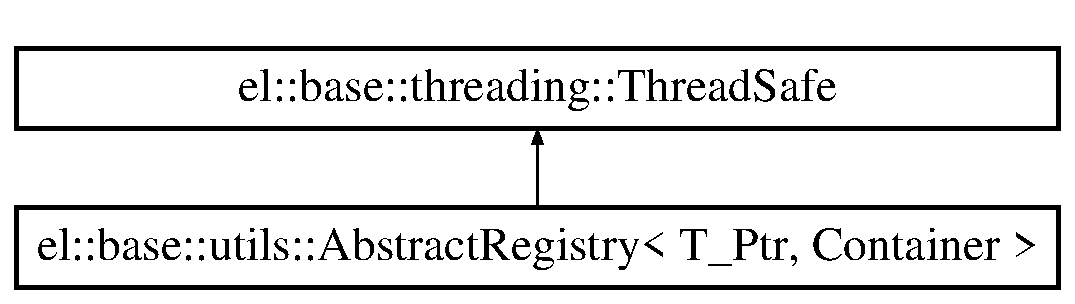
\includegraphics[height=2.000000cm]{classel_1_1base_1_1utils_1_1_abstract_registry}
\end{center}
\end{figure}
\subsection*{Public Types}
\begin{DoxyCompactItemize}
\item 
typedef Container\+::iterator \hyperlink{classel_1_1base_1_1utils_1_1_abstract_registry_a58d0536c748633afd3f7c237b63a9a7c}{iterator}
\item 
typedef Container\+::const\+\_\+iterator \hyperlink{classel_1_1base_1_1utils_1_1_abstract_registry_a3bbf19b112c067cb1a02a82b003cc7e2}{const\+\_\+iterator}
\end{DoxyCompactItemize}
\subsection*{Public Member Functions}
\begin{DoxyCompactItemize}
\item 
\hyperlink{classel_1_1base_1_1utils_1_1_abstract_registry_afe13c67ebd1ed1aa72845926894dffa2}{Abstract\+Registry} (void)
\begin{DoxyCompactList}\small\item\em Default constructor. \end{DoxyCompactList}\item 
\hyperlink{classel_1_1base_1_1utils_1_1_abstract_registry_a9f468010439d491e90419f9334afcdba}{Abstract\+Registry} (\hyperlink{classel_1_1base_1_1utils_1_1_abstract_registry}{Abstract\+Registry} \&\&sr)
\begin{DoxyCompactList}\small\item\em Move constructor that is useful for base classes. \end{DoxyCompactList}\item 
bool \hyperlink{classel_1_1base_1_1utils_1_1_abstract_registry_ac3e648dc0caa8914f8604650f00bc94b}{operator==} (const \hyperlink{classel_1_1base_1_1utils_1_1_abstract_registry}{Abstract\+Registry}$<$ T\+\_\+\+Ptr, Container $>$ \&other)
\item 
bool \hyperlink{classel_1_1base_1_1utils_1_1_abstract_registry_a35de8807521651c85acb26532a2623e1}{operator!=} (const \hyperlink{classel_1_1base_1_1utils_1_1_abstract_registry}{Abstract\+Registry}$<$ T\+\_\+\+Ptr, Container $>$ \&other)
\item 
\hyperlink{classel_1_1base_1_1utils_1_1_abstract_registry}{Abstract\+Registry} \& \hyperlink{classel_1_1base_1_1utils_1_1_abstract_registry_a5727a3cadeee6a2b10d8f46fb91956e7}{operator=} (\hyperlink{classel_1_1base_1_1utils_1_1_abstract_registry}{Abstract\+Registry} \&\&sr)
\begin{DoxyCompactList}\small\item\em Assignment move operator. \end{DoxyCompactList}\item 
virtual \hyperlink{classel_1_1base_1_1utils_1_1_abstract_registry_a6ee2c4166629bb16515cc00b738dee65}{$\sim$\+Abstract\+Registry} (void)
\item 
virtual \hyperlink{classel_1_1base_1_1utils_1_1_abstract_registry_a58d0536c748633afd3f7c237b63a9a7c}{iterator} \hyperlink{classel_1_1base_1_1utils_1_1_abstract_registry_a4ad971b1dddff996d327452d852e55b2}{begin} (void) \hyperlink{easylogging_09_09_8h_a2f812449f8d3355cf5b03ceb2ee5021b}{E\+L\+P\+P\+\_\+\+F\+I\+N\+A\+L}
\item 
virtual \hyperlink{classel_1_1base_1_1utils_1_1_abstract_registry_a58d0536c748633afd3f7c237b63a9a7c}{iterator} \hyperlink{classel_1_1base_1_1utils_1_1_abstract_registry_a67c40207c171f23ad50a71db819e84f9}{end} (void) \hyperlink{easylogging_09_09_8h_a2f812449f8d3355cf5b03ceb2ee5021b}{E\+L\+P\+P\+\_\+\+F\+I\+N\+A\+L}
\item 
virtual \hyperlink{classel_1_1base_1_1utils_1_1_abstract_registry_a3bbf19b112c067cb1a02a82b003cc7e2}{const\+\_\+iterator} \hyperlink{classel_1_1base_1_1utils_1_1_abstract_registry_a37f743184e808d7c0028e21e0d0898bb}{cbegin} (void) const \hyperlink{easylogging_09_09_8h_a2f812449f8d3355cf5b03ceb2ee5021b}{E\+L\+P\+P\+\_\+\+F\+I\+N\+A\+L}
\item 
virtual \hyperlink{classel_1_1base_1_1utils_1_1_abstract_registry_a3bbf19b112c067cb1a02a82b003cc7e2}{const\+\_\+iterator} \hyperlink{classel_1_1base_1_1utils_1_1_abstract_registry_ad3ee081b4b25c5d77f971f949bdb9158}{cend} (void) const \hyperlink{easylogging_09_09_8h_a2f812449f8d3355cf5b03ceb2ee5021b}{E\+L\+P\+P\+\_\+\+F\+I\+N\+A\+L}
\item 
virtual bool \hyperlink{classel_1_1base_1_1utils_1_1_abstract_registry_a43ff6484b778c298416c482c07a4df3f}{empty} (void) const \hyperlink{easylogging_09_09_8h_a2f812449f8d3355cf5b03ceb2ee5021b}{E\+L\+P\+P\+\_\+\+F\+I\+N\+A\+L}
\item 
virtual std\+::size\+\_\+t \hyperlink{classel_1_1base_1_1utils_1_1_abstract_registry_a58a7b8ea964bdf6008701dcfb6609ca5}{size} (void) const \hyperlink{easylogging_09_09_8h_a2f812449f8d3355cf5b03ceb2ee5021b}{E\+L\+P\+P\+\_\+\+F\+I\+N\+A\+L}
\item 
virtual Container \& \hyperlink{classel_1_1base_1_1utils_1_1_abstract_registry_a072859d3728a75f910c2898f62fd12da}{list} (void) \hyperlink{easylogging_09_09_8h_a2f812449f8d3355cf5b03ceb2ee5021b}{E\+L\+P\+P\+\_\+\+F\+I\+N\+A\+L}
\begin{DoxyCompactList}\small\item\em Returns underlying container by reference. \end{DoxyCompactList}\item 
virtual const Container \& \hyperlink{classel_1_1base_1_1utils_1_1_abstract_registry_a1c3da2af9177cbfae6f10b9e5dbe615c}{list} (void) const \hyperlink{easylogging_09_09_8h_a2f812449f8d3355cf5b03ceb2ee5021b}{E\+L\+P\+P\+\_\+\+F\+I\+N\+A\+L}
\begin{DoxyCompactList}\small\item\em Returns underlying container by constant reference. \end{DoxyCompactList}\item 
virtual void \hyperlink{classel_1_1base_1_1utils_1_1_abstract_registry_a19223bc1fea48dbe6b47b4879aa4672f}{unregister\+All} (void)=0
\begin{DoxyCompactList}\small\item\em Unregisters all the pointers from current repository. \end{DoxyCompactList}\end{DoxyCompactItemize}
\subsection*{Protected Member Functions}
\begin{DoxyCompactItemize}
\item 
virtual void \hyperlink{classel_1_1base_1_1utils_1_1_abstract_registry_aaf42dab7089a9b1198e2920983ca82bb}{deep\+Copy} (const \hyperlink{classel_1_1base_1_1utils_1_1_abstract_registry}{Abstract\+Registry}$<$ T\+\_\+\+Ptr, Container $>$ \&)=0
\item 
void \hyperlink{classel_1_1base_1_1utils_1_1_abstract_registry_a529677fb42e78d03c36cdea49f8877c9}{reinit\+Deep\+Copy} (const \hyperlink{classel_1_1base_1_1utils_1_1_abstract_registry}{Abstract\+Registry}$<$ T\+\_\+\+Ptr, Container $>$ \&sr)
\end{DoxyCompactItemize}


\subsection{Detailed Description}
\subsubsection*{template$<$typename T\+\_\+\+Ptr, typename Container$>$class el\+::base\+::utils\+::\+Abstract\+Registry$<$ T\+\_\+\+Ptr, Container $>$}

Abstract registry (aka repository) that provides basic interface for pointer repository specified by T\+\_\+\+Ptr type. 

Most of the functions are virtual final methods but anything implementing this abstract class should implement \hyperlink{classel_1_1base_1_1utils_1_1_abstract_registry_a19223bc1fea48dbe6b47b4879aa4672f}{unregister\+All()} and \hyperlink{classel_1_1base_1_1utils_1_1_abstract_registry_aaf42dab7089a9b1198e2920983ca82bb}{deep\+Copy(const Abstract\+Registry$<$\+T\+\_\+\+Ptr, Container$>$\&)} and write register\+New() method according to container and few more methods; get() to find element, unregister() to unregister single entry. Please note that this is thread-\/unsafe and should also implement thread-\/safety mechanisms in implementation. 

Definition at line 1814 of file easylogging++.\+h.



\subsection{Member Typedef Documentation}
\hypertarget{classel_1_1base_1_1utils_1_1_abstract_registry_a3bbf19b112c067cb1a02a82b003cc7e2}{}\index{el\+::base\+::utils\+::\+Abstract\+Registry@{el\+::base\+::utils\+::\+Abstract\+Registry}!const\+\_\+iterator@{const\+\_\+iterator}}
\index{const\+\_\+iterator@{const\+\_\+iterator}!el\+::base\+::utils\+::\+Abstract\+Registry@{el\+::base\+::utils\+::\+Abstract\+Registry}}
\subsubsection[{const\+\_\+iterator}]{\setlength{\rightskip}{0pt plus 5cm}template$<$typename T\+\_\+\+Ptr, typename Container$>$ typedef Container\+::const\+\_\+iterator {\bf el\+::base\+::utils\+::\+Abstract\+Registry}$<$ T\+\_\+\+Ptr, Container $>$\+::{\bf const\+\_\+iterator}}\label{classel_1_1base_1_1utils_1_1_abstract_registry_a3bbf19b112c067cb1a02a82b003cc7e2}


Definition at line 1817 of file easylogging++.\+h.

\hypertarget{classel_1_1base_1_1utils_1_1_abstract_registry_a58d0536c748633afd3f7c237b63a9a7c}{}\index{el\+::base\+::utils\+::\+Abstract\+Registry@{el\+::base\+::utils\+::\+Abstract\+Registry}!iterator@{iterator}}
\index{iterator@{iterator}!el\+::base\+::utils\+::\+Abstract\+Registry@{el\+::base\+::utils\+::\+Abstract\+Registry}}
\subsubsection[{iterator}]{\setlength{\rightskip}{0pt plus 5cm}template$<$typename T\+\_\+\+Ptr, typename Container$>$ typedef Container\+::iterator {\bf el\+::base\+::utils\+::\+Abstract\+Registry}$<$ T\+\_\+\+Ptr, Container $>$\+::{\bf iterator}}\label{classel_1_1base_1_1utils_1_1_abstract_registry_a58d0536c748633afd3f7c237b63a9a7c}


Definition at line 1816 of file easylogging++.\+h.



\subsection{Constructor \& Destructor Documentation}
\hypertarget{classel_1_1base_1_1utils_1_1_abstract_registry_afe13c67ebd1ed1aa72845926894dffa2}{}\index{el\+::base\+::utils\+::\+Abstract\+Registry@{el\+::base\+::utils\+::\+Abstract\+Registry}!Abstract\+Registry@{Abstract\+Registry}}
\index{Abstract\+Registry@{Abstract\+Registry}!el\+::base\+::utils\+::\+Abstract\+Registry@{el\+::base\+::utils\+::\+Abstract\+Registry}}
\subsubsection[{Abstract\+Registry}]{\setlength{\rightskip}{0pt plus 5cm}template$<$typename T\+\_\+\+Ptr, typename Container$>$ {\bf el\+::base\+::utils\+::\+Abstract\+Registry}$<$ T\+\_\+\+Ptr, Container $>$\+::{\bf Abstract\+Registry} (
\begin{DoxyParamCaption}
\item[{void}]{}
\end{DoxyParamCaption}
)\hspace{0.3cm}{\ttfamily [inline]}}\label{classel_1_1base_1_1utils_1_1_abstract_registry_afe13c67ebd1ed1aa72845926894dffa2}


Default constructor. 



Definition at line 1820 of file easylogging++.\+h.

\hypertarget{classel_1_1base_1_1utils_1_1_abstract_registry_a9f468010439d491e90419f9334afcdba}{}\index{el\+::base\+::utils\+::\+Abstract\+Registry@{el\+::base\+::utils\+::\+Abstract\+Registry}!Abstract\+Registry@{Abstract\+Registry}}
\index{Abstract\+Registry@{Abstract\+Registry}!el\+::base\+::utils\+::\+Abstract\+Registry@{el\+::base\+::utils\+::\+Abstract\+Registry}}
\subsubsection[{Abstract\+Registry}]{\setlength{\rightskip}{0pt plus 5cm}template$<$typename T\+\_\+\+Ptr, typename Container$>$ {\bf el\+::base\+::utils\+::\+Abstract\+Registry}$<$ T\+\_\+\+Ptr, Container $>$\+::{\bf Abstract\+Registry} (
\begin{DoxyParamCaption}
\item[{{\bf Abstract\+Registry}$<$ T\+\_\+\+Ptr, Container $>$ \&\&}]{sr}
\end{DoxyParamCaption}
)\hspace{0.3cm}{\ttfamily [inline]}}\label{classel_1_1base_1_1utils_1_1_abstract_registry_a9f468010439d491e90419f9334afcdba}


Move constructor that is useful for base classes. 



Definition at line 1823 of file easylogging++.\+h.

\hypertarget{classel_1_1base_1_1utils_1_1_abstract_registry_a6ee2c4166629bb16515cc00b738dee65}{}\index{el\+::base\+::utils\+::\+Abstract\+Registry@{el\+::base\+::utils\+::\+Abstract\+Registry}!````~Abstract\+Registry@{$\sim$\+Abstract\+Registry}}
\index{````~Abstract\+Registry@{$\sim$\+Abstract\+Registry}!el\+::base\+::utils\+::\+Abstract\+Registry@{el\+::base\+::utils\+::\+Abstract\+Registry}}
\subsubsection[{$\sim$\+Abstract\+Registry}]{\setlength{\rightskip}{0pt plus 5cm}template$<$typename T\+\_\+\+Ptr, typename Container$>$ virtual {\bf el\+::base\+::utils\+::\+Abstract\+Registry}$<$ T\+\_\+\+Ptr, Container $>$\+::$\sim${\bf Abstract\+Registry} (
\begin{DoxyParamCaption}
\item[{void}]{}
\end{DoxyParamCaption}
)\hspace{0.3cm}{\ttfamily [inline]}, {\ttfamily [virtual]}}\label{classel_1_1base_1_1utils_1_1_abstract_registry_a6ee2c4166629bb16515cc00b738dee65}


Definition at line 1865 of file easylogging++.\+h.



\subsection{Member Function Documentation}
\hypertarget{classel_1_1base_1_1utils_1_1_abstract_registry_a4ad971b1dddff996d327452d852e55b2}{}\index{el\+::base\+::utils\+::\+Abstract\+Registry@{el\+::base\+::utils\+::\+Abstract\+Registry}!begin@{begin}}
\index{begin@{begin}!el\+::base\+::utils\+::\+Abstract\+Registry@{el\+::base\+::utils\+::\+Abstract\+Registry}}
\subsubsection[{begin}]{\setlength{\rightskip}{0pt plus 5cm}template$<$typename T\+\_\+\+Ptr, typename Container$>$ virtual {\bf iterator} {\bf el\+::base\+::utils\+::\+Abstract\+Registry}$<$ T\+\_\+\+Ptr, Container $>$\+::begin (
\begin{DoxyParamCaption}
\item[{void}]{}
\end{DoxyParamCaption}
)\hspace{0.3cm}{\ttfamily [inline]}, {\ttfamily [virtual]}}\label{classel_1_1base_1_1utils_1_1_abstract_registry_a4ad971b1dddff996d327452d852e55b2}
\begin{DoxyReturn}{Returns}
Iterator pointer from start of repository 
\end{DoxyReturn}


Definition at line 1869 of file easylogging++.\+h.

\hypertarget{classel_1_1base_1_1utils_1_1_abstract_registry_a37f743184e808d7c0028e21e0d0898bb}{}\index{el\+::base\+::utils\+::\+Abstract\+Registry@{el\+::base\+::utils\+::\+Abstract\+Registry}!cbegin@{cbegin}}
\index{cbegin@{cbegin}!el\+::base\+::utils\+::\+Abstract\+Registry@{el\+::base\+::utils\+::\+Abstract\+Registry}}
\subsubsection[{cbegin}]{\setlength{\rightskip}{0pt plus 5cm}template$<$typename T\+\_\+\+Ptr, typename Container$>$ virtual {\bf const\+\_\+iterator} {\bf el\+::base\+::utils\+::\+Abstract\+Registry}$<$ T\+\_\+\+Ptr, Container $>$\+::cbegin (
\begin{DoxyParamCaption}
\item[{void}]{}
\end{DoxyParamCaption}
) const\hspace{0.3cm}{\ttfamily [inline]}, {\ttfamily [virtual]}}\label{classel_1_1base_1_1utils_1_1_abstract_registry_a37f743184e808d7c0028e21e0d0898bb}
\begin{DoxyReturn}{Returns}
Constant iterator pointer from start of repository 
\end{DoxyReturn}


Definition at line 1880 of file easylogging++.\+h.

\hypertarget{classel_1_1base_1_1utils_1_1_abstract_registry_ad3ee081b4b25c5d77f971f949bdb9158}{}\index{el\+::base\+::utils\+::\+Abstract\+Registry@{el\+::base\+::utils\+::\+Abstract\+Registry}!cend@{cend}}
\index{cend@{cend}!el\+::base\+::utils\+::\+Abstract\+Registry@{el\+::base\+::utils\+::\+Abstract\+Registry}}
\subsubsection[{cend}]{\setlength{\rightskip}{0pt plus 5cm}template$<$typename T\+\_\+\+Ptr, typename Container$>$ virtual {\bf const\+\_\+iterator} {\bf el\+::base\+::utils\+::\+Abstract\+Registry}$<$ T\+\_\+\+Ptr, Container $>$\+::cend (
\begin{DoxyParamCaption}
\item[{void}]{}
\end{DoxyParamCaption}
) const\hspace{0.3cm}{\ttfamily [inline]}, {\ttfamily [virtual]}}\label{classel_1_1base_1_1utils_1_1_abstract_registry_ad3ee081b4b25c5d77f971f949bdb9158}
\begin{DoxyReturn}{Returns}
End of repository 
\end{DoxyReturn}


Definition at line 1885 of file easylogging++.\+h.

\hypertarget{classel_1_1base_1_1utils_1_1_abstract_registry_aaf42dab7089a9b1198e2920983ca82bb}{}\index{el\+::base\+::utils\+::\+Abstract\+Registry@{el\+::base\+::utils\+::\+Abstract\+Registry}!deep\+Copy@{deep\+Copy}}
\index{deep\+Copy@{deep\+Copy}!el\+::base\+::utils\+::\+Abstract\+Registry@{el\+::base\+::utils\+::\+Abstract\+Registry}}
\subsubsection[{deep\+Copy}]{\setlength{\rightskip}{0pt plus 5cm}template$<$typename T\+\_\+\+Ptr, typename Container$>$ virtual void {\bf el\+::base\+::utils\+::\+Abstract\+Registry}$<$ T\+\_\+\+Ptr, Container $>$\+::deep\+Copy (
\begin{DoxyParamCaption}
\item[{const {\bf Abstract\+Registry}$<$ T\+\_\+\+Ptr, Container $>$ \&}]{}
\end{DoxyParamCaption}
)\hspace{0.3cm}{\ttfamily [protected]}, {\ttfamily [pure virtual]}}\label{classel_1_1base_1_1utils_1_1_abstract_registry_aaf42dab7089a9b1198e2920983ca82bb}
\hypertarget{classel_1_1base_1_1utils_1_1_abstract_registry_a43ff6484b778c298416c482c07a4df3f}{}\index{el\+::base\+::utils\+::\+Abstract\+Registry@{el\+::base\+::utils\+::\+Abstract\+Registry}!empty@{empty}}
\index{empty@{empty}!el\+::base\+::utils\+::\+Abstract\+Registry@{el\+::base\+::utils\+::\+Abstract\+Registry}}
\subsubsection[{empty}]{\setlength{\rightskip}{0pt plus 5cm}template$<$typename T\+\_\+\+Ptr, typename Container$>$ virtual bool {\bf el\+::base\+::utils\+::\+Abstract\+Registry}$<$ T\+\_\+\+Ptr, Container $>$\+::empty (
\begin{DoxyParamCaption}
\item[{void}]{}
\end{DoxyParamCaption}
) const\hspace{0.3cm}{\ttfamily [inline]}, {\ttfamily [virtual]}}\label{classel_1_1base_1_1utils_1_1_abstract_registry_a43ff6484b778c298416c482c07a4df3f}
\begin{DoxyReturn}{Returns}
Whether or not repository is empty 
\end{DoxyReturn}


Definition at line 1890 of file easylogging++.\+h.

\hypertarget{classel_1_1base_1_1utils_1_1_abstract_registry_a67c40207c171f23ad50a71db819e84f9}{}\index{el\+::base\+::utils\+::\+Abstract\+Registry@{el\+::base\+::utils\+::\+Abstract\+Registry}!end@{end}}
\index{end@{end}!el\+::base\+::utils\+::\+Abstract\+Registry@{el\+::base\+::utils\+::\+Abstract\+Registry}}
\subsubsection[{end}]{\setlength{\rightskip}{0pt plus 5cm}template$<$typename T\+\_\+\+Ptr, typename Container$>$ virtual {\bf iterator} {\bf el\+::base\+::utils\+::\+Abstract\+Registry}$<$ T\+\_\+\+Ptr, Container $>$\+::end (
\begin{DoxyParamCaption}
\item[{void}]{}
\end{DoxyParamCaption}
)\hspace{0.3cm}{\ttfamily [inline]}, {\ttfamily [virtual]}}\label{classel_1_1base_1_1utils_1_1_abstract_registry_a67c40207c171f23ad50a71db819e84f9}
\begin{DoxyReturn}{Returns}
Iterator pointer from end of repository 
\end{DoxyReturn}


Definition at line 1874 of file easylogging++.\+h.

\hypertarget{classel_1_1base_1_1utils_1_1_abstract_registry_a072859d3728a75f910c2898f62fd12da}{}\index{el\+::base\+::utils\+::\+Abstract\+Registry@{el\+::base\+::utils\+::\+Abstract\+Registry}!list@{list}}
\index{list@{list}!el\+::base\+::utils\+::\+Abstract\+Registry@{el\+::base\+::utils\+::\+Abstract\+Registry}}
\subsubsection[{list}]{\setlength{\rightskip}{0pt plus 5cm}template$<$typename T\+\_\+\+Ptr, typename Container$>$ virtual Container\& {\bf el\+::base\+::utils\+::\+Abstract\+Registry}$<$ T\+\_\+\+Ptr, Container $>$\+::list (
\begin{DoxyParamCaption}
\item[{void}]{}
\end{DoxyParamCaption}
)\hspace{0.3cm}{\ttfamily [inline]}, {\ttfamily [virtual]}}\label{classel_1_1base_1_1utils_1_1_abstract_registry_a072859d3728a75f910c2898f62fd12da}


Returns underlying container by reference. 



Definition at line 1900 of file easylogging++.\+h.

\hypertarget{classel_1_1base_1_1utils_1_1_abstract_registry_a1c3da2af9177cbfae6f10b9e5dbe615c}{}\index{el\+::base\+::utils\+::\+Abstract\+Registry@{el\+::base\+::utils\+::\+Abstract\+Registry}!list@{list}}
\index{list@{list}!el\+::base\+::utils\+::\+Abstract\+Registry@{el\+::base\+::utils\+::\+Abstract\+Registry}}
\subsubsection[{list}]{\setlength{\rightskip}{0pt plus 5cm}template$<$typename T\+\_\+\+Ptr, typename Container$>$ virtual const Container\& {\bf el\+::base\+::utils\+::\+Abstract\+Registry}$<$ T\+\_\+\+Ptr, Container $>$\+::list (
\begin{DoxyParamCaption}
\item[{void}]{}
\end{DoxyParamCaption}
) const\hspace{0.3cm}{\ttfamily [inline]}, {\ttfamily [virtual]}}\label{classel_1_1base_1_1utils_1_1_abstract_registry_a1c3da2af9177cbfae6f10b9e5dbe615c}


Returns underlying container by constant reference. 



Definition at line 1905 of file easylogging++.\+h.

\hypertarget{classel_1_1base_1_1utils_1_1_abstract_registry_a35de8807521651c85acb26532a2623e1}{}\index{el\+::base\+::utils\+::\+Abstract\+Registry@{el\+::base\+::utils\+::\+Abstract\+Registry}!operator"!=@{operator"!=}}
\index{operator"!=@{operator"!=}!el\+::base\+::utils\+::\+Abstract\+Registry@{el\+::base\+::utils\+::\+Abstract\+Registry}}
\subsubsection[{operator"!=}]{\setlength{\rightskip}{0pt plus 5cm}template$<$typename T\+\_\+\+Ptr, typename Container$>$ bool {\bf el\+::base\+::utils\+::\+Abstract\+Registry}$<$ T\+\_\+\+Ptr, Container $>$\+::operator!= (
\begin{DoxyParamCaption}
\item[{const {\bf Abstract\+Registry}$<$ T\+\_\+\+Ptr, Container $>$ \&}]{other}
\end{DoxyParamCaption}
)\hspace{0.3cm}{\ttfamily [inline]}}\label{classel_1_1base_1_1utils_1_1_abstract_registry_a35de8807521651c85acb26532a2623e1}


Definition at line 1843 of file easylogging++.\+h.

\hypertarget{classel_1_1base_1_1utils_1_1_abstract_registry_a5727a3cadeee6a2b10d8f46fb91956e7}{}\index{el\+::base\+::utils\+::\+Abstract\+Registry@{el\+::base\+::utils\+::\+Abstract\+Registry}!operator=@{operator=}}
\index{operator=@{operator=}!el\+::base\+::utils\+::\+Abstract\+Registry@{el\+::base\+::utils\+::\+Abstract\+Registry}}
\subsubsection[{operator=}]{\setlength{\rightskip}{0pt plus 5cm}template$<$typename T\+\_\+\+Ptr, typename Container$>$ {\bf Abstract\+Registry}\& {\bf el\+::base\+::utils\+::\+Abstract\+Registry}$<$ T\+\_\+\+Ptr, Container $>$\+::operator= (
\begin{DoxyParamCaption}
\item[{{\bf Abstract\+Registry}$<$ T\+\_\+\+Ptr, Container $>$ \&\&}]{sr}
\end{DoxyParamCaption}
)\hspace{0.3cm}{\ttfamily [inline]}}\label{classel_1_1base_1_1utils_1_1_abstract_registry_a5727a3cadeee6a2b10d8f46fb91956e7}


Assignment move operator. 



Definition at line 1856 of file easylogging++.\+h.

\hypertarget{classel_1_1base_1_1utils_1_1_abstract_registry_ac3e648dc0caa8914f8604650f00bc94b}{}\index{el\+::base\+::utils\+::\+Abstract\+Registry@{el\+::base\+::utils\+::\+Abstract\+Registry}!operator==@{operator==}}
\index{operator==@{operator==}!el\+::base\+::utils\+::\+Abstract\+Registry@{el\+::base\+::utils\+::\+Abstract\+Registry}}
\subsubsection[{operator==}]{\setlength{\rightskip}{0pt plus 5cm}template$<$typename T\+\_\+\+Ptr, typename Container$>$ bool {\bf el\+::base\+::utils\+::\+Abstract\+Registry}$<$ T\+\_\+\+Ptr, Container $>$\+::operator== (
\begin{DoxyParamCaption}
\item[{const {\bf Abstract\+Registry}$<$ T\+\_\+\+Ptr, Container $>$ \&}]{other}
\end{DoxyParamCaption}
)\hspace{0.3cm}{\ttfamily [inline]}}\label{classel_1_1base_1_1utils_1_1_abstract_registry_ac3e648dc0caa8914f8604650f00bc94b}


Definition at line 1831 of file easylogging++.\+h.

\hypertarget{classel_1_1base_1_1utils_1_1_abstract_registry_a529677fb42e78d03c36cdea49f8877c9}{}\index{el\+::base\+::utils\+::\+Abstract\+Registry@{el\+::base\+::utils\+::\+Abstract\+Registry}!reinit\+Deep\+Copy@{reinit\+Deep\+Copy}}
\index{reinit\+Deep\+Copy@{reinit\+Deep\+Copy}!el\+::base\+::utils\+::\+Abstract\+Registry@{el\+::base\+::utils\+::\+Abstract\+Registry}}
\subsubsection[{reinit\+Deep\+Copy}]{\setlength{\rightskip}{0pt plus 5cm}template$<$typename T\+\_\+\+Ptr, typename Container$>$ void {\bf el\+::base\+::utils\+::\+Abstract\+Registry}$<$ T\+\_\+\+Ptr, Container $>$\+::reinit\+Deep\+Copy (
\begin{DoxyParamCaption}
\item[{const {\bf Abstract\+Registry}$<$ T\+\_\+\+Ptr, Container $>$ \&}]{sr}
\end{DoxyParamCaption}
)\hspace{0.3cm}{\ttfamily [inline]}, {\ttfamily [protected]}}\label{classel_1_1base_1_1utils_1_1_abstract_registry_a529677fb42e78d03c36cdea49f8877c9}


Definition at line 1914 of file easylogging++.\+h.

\hypertarget{classel_1_1base_1_1utils_1_1_abstract_registry_a58a7b8ea964bdf6008701dcfb6609ca5}{}\index{el\+::base\+::utils\+::\+Abstract\+Registry@{el\+::base\+::utils\+::\+Abstract\+Registry}!size@{size}}
\index{size@{size}!el\+::base\+::utils\+::\+Abstract\+Registry@{el\+::base\+::utils\+::\+Abstract\+Registry}}
\subsubsection[{size}]{\setlength{\rightskip}{0pt plus 5cm}template$<$typename T\+\_\+\+Ptr, typename Container$>$ virtual std\+::size\+\_\+t {\bf el\+::base\+::utils\+::\+Abstract\+Registry}$<$ T\+\_\+\+Ptr, Container $>$\+::size (
\begin{DoxyParamCaption}
\item[{void}]{}
\end{DoxyParamCaption}
) const\hspace{0.3cm}{\ttfamily [inline]}, {\ttfamily [virtual]}}\label{classel_1_1base_1_1utils_1_1_abstract_registry_a58a7b8ea964bdf6008701dcfb6609ca5}
\begin{DoxyReturn}{Returns}
Size of repository 
\end{DoxyReturn}


Definition at line 1895 of file easylogging++.\+h.

\hypertarget{classel_1_1base_1_1utils_1_1_abstract_registry_a19223bc1fea48dbe6b47b4879aa4672f}{}\index{el\+::base\+::utils\+::\+Abstract\+Registry@{el\+::base\+::utils\+::\+Abstract\+Registry}!unregister\+All@{unregister\+All}}
\index{unregister\+All@{unregister\+All}!el\+::base\+::utils\+::\+Abstract\+Registry@{el\+::base\+::utils\+::\+Abstract\+Registry}}
\subsubsection[{unregister\+All}]{\setlength{\rightskip}{0pt plus 5cm}template$<$typename T\+\_\+\+Ptr, typename Container$>$ virtual void {\bf el\+::base\+::utils\+::\+Abstract\+Registry}$<$ T\+\_\+\+Ptr, Container $>$\+::unregister\+All (
\begin{DoxyParamCaption}
\item[{void}]{}
\end{DoxyParamCaption}
)\hspace{0.3cm}{\ttfamily [pure virtual]}}\label{classel_1_1base_1_1utils_1_1_abstract_registry_a19223bc1fea48dbe6b47b4879aa4672f}


Unregisters all the pointers from current repository. 



Implemented in \hyperlink{classel_1_1base_1_1utils_1_1_registry_with_pred_a66b4eca5bb71f3fa3f0737105a00890c}{el\+::base\+::utils\+::\+Registry\+With\+Pred$<$ T\+\_\+\+Ptr, Pred $>$}, \hyperlink{classel_1_1base_1_1utils_1_1_registry_with_pred_a66b4eca5bb71f3fa3f0737105a00890c}{el\+::base\+::utils\+::\+Registry\+With\+Pred$<$ Configuration, Configuration\+::\+Predicate $>$}, \hyperlink{classel_1_1base_1_1utils_1_1_registry_with_pred_a66b4eca5bb71f3fa3f0737105a00890c}{el\+::base\+::utils\+::\+Registry\+With\+Pred$<$ base\+::\+Hit\+Counter, base\+::\+Hit\+Counter\+::\+Predicate $>$}, \hyperlink{classel_1_1base_1_1utils_1_1_registry_ac40e62ddf5017beb91c28b472c9628c2}{el\+::base\+::utils\+::\+Registry$<$ T\+\_\+\+Ptr, T\+\_\+\+Key $>$}, and \hyperlink{classel_1_1base_1_1utils_1_1_registry_ac40e62ddf5017beb91c28b472c9628c2}{el\+::base\+::utils\+::\+Registry$<$ Logger, std\+::string $>$}.



The documentation for this class was generated from the following file\+:\begin{DoxyCompactItemize}
\item 
lib/\hyperlink{easylogging_09_09_8h}{easylogging++.\+h}\end{DoxyCompactItemize}

\hypertarget{class_abstract_scheduler}{}\section{Abstract\+Scheduler Class Reference}
\label{class_abstract_scheduler}\index{Abstract\+Scheduler@{Abstract\+Scheduler}}


{\ttfamily \#include $<$Abstract\+Scheduler.\+h$>$}

Inheritance diagram for Abstract\+Scheduler\+:\begin{figure}[H]
\begin{center}
\leavevmode
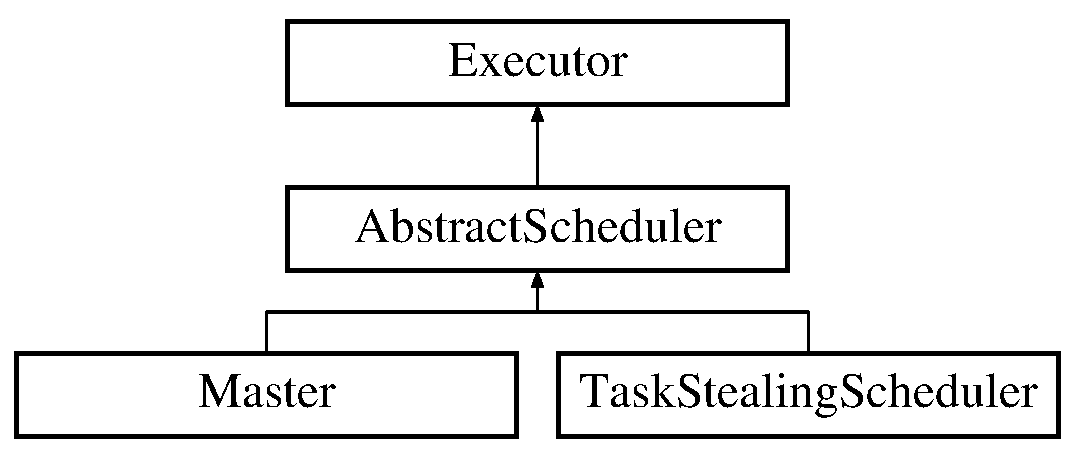
\includegraphics[height=3.000000cm]{class_abstract_scheduler}
\end{center}
\end{figure}
\subsection*{Public Member Functions}
\begin{DoxyCompactItemize}
\item 
\hyperlink{class_abstract_scheduler_addaf6f185aefd7304df9a3cc4e020b00}{Abstract\+Scheduler} (\hyperlink{class_scheduling_strategy}{Scheduling\+Strategy} $\ast$\hyperlink{class_abstract_scheduler_a7dd11eee79bfb44c820d6c28480fd0c7}{scheduling\+\_\+strategy}, \hyperlink{class_data_mining}{Data\+Mining} $\ast$\hyperlink{class_abstract_scheduler_a6e281d90fa4b965779cd13eabf7d0249}{data\+\_\+miner}, int \hyperlink{class_executor_a33c24e2887b4d9c4ef7f3566d3bc803e}{rank}, int \hyperlink{class_executor_a4e798bde66d26fe200de7e8d2b54e915}{number\+\_\+of\+\_\+processors})
\item 
virtual \hyperlink{class_abstract_scheduler_a1f8fb108f61bf092407c6fba1afb8578}{$\sim$\+Abstract\+Scheduler} ()
\item 
virtual void \hyperlink{class_abstract_scheduler_a5171d8f76ad183ea1d0f6bb393293be8}{place\+\_\+task} (\hyperlink{_types_8h_a0c77930ab3818a1680c59353f627fba8}{Task} task)
\item 
int \hyperlink{class_abstract_scheduler_a205d6e6fd08ffbc000a79944f9f59853}{get\+\_\+rank} ()
\end{DoxyCompactItemize}
\subsection*{Protected Member Functions}
\begin{DoxyCompactItemize}
\item 
virtual void \hyperlink{class_abstract_scheduler_a284ad11479af671abf7130abb5f69992}{preprocessing} (int argc, char $\ast$argv\mbox{[}$\,$\mbox{]}, \hyperlink{_types_8h_a0c77930ab3818a1680c59353f627fba8}{Task} $\ast$buffer, int $\ast$initial\+\_\+tasks\+\_\+number)
\item 
virtual void \hyperlink{class_abstract_scheduler_a3c2b64a8a6de2687258dea9d58769792}{postprocessing} ()
\item 
virtual void \hyperlink{class_abstract_scheduler_ab5f9142ccfc130e91fa6d92c7d3d7469}{run} ()=0
\item 
virtual bool \hyperlink{class_abstract_scheduler_acc7d6dc38aa80ca77ac892c74b915432}{is\+\_\+finish} ()=0
\end{DoxyCompactItemize}
\subsection*{Protected Attributes}
\begin{DoxyCompactItemize}
\item 
\hyperlink{class_scheduling_strategy}{Scheduling\+Strategy} $\ast$ \hyperlink{class_abstract_scheduler_a7dd11eee79bfb44c820d6c28480fd0c7}{scheduling\+\_\+strategy}
\item 
\hyperlink{class_data_mining}{Data\+Mining} $\ast$ \hyperlink{class_abstract_scheduler_a6e281d90fa4b965779cd13eabf7d0249}{data\+\_\+miner}
\item 
\hyperlink{class_scheduling_strategy_evaluator}{Scheduling\+Strategy\+Evaluator} $\ast$ \hyperlink{class_abstract_scheduler_a5f95e61e03441ca92c6ba8f434be7fe0}{scheduling\+Strategy\+Evaluator}
\end{DoxyCompactItemize}
\subsection*{Additional Inherited Members}


\subsection{Detailed Description}
The abstract \hyperlink{class_abstract_scheduler}{Abstract\+Scheduler} class is the base class for all types of scheduler objects like master-\/worker scheduler or task stealing scheduler and inherits from the \hyperlink{class_executor}{Executor} class. Subclasses have to override the \hyperlink{class_abstract_scheduler_ab5f9142ccfc130e91fa6d92c7d3d7469}{run()} and the \hyperlink{class_abstract_scheduler_acc7d6dc38aa80ca77ac892c74b915432}{is\+\_\+finish()} function. The preprocessing and the postprocessing function call the code\+\_\+proprocessing\+\_\+master() and the \hyperlink{_scientific_code_8cpp_a2dfc976aa95c961d1f76ce3f7c56f243}{code\+\_\+postprocessing\+\_\+master()} functions on the code interface.

\begin{DoxyAuthor}{Author}
Fabio Broghammer 
\end{DoxyAuthor}
\begin{DoxyVersion}{Version}
1.\+0 
\end{DoxyVersion}


Definition at line 18 of file Abstract\+Scheduler.\+h.



\subsection{Constructor \& Destructor Documentation}
\hypertarget{class_abstract_scheduler_addaf6f185aefd7304df9a3cc4e020b00}{}\index{Abstract\+Scheduler@{Abstract\+Scheduler}!Abstract\+Scheduler@{Abstract\+Scheduler}}
\index{Abstract\+Scheduler@{Abstract\+Scheduler}!Abstract\+Scheduler@{Abstract\+Scheduler}}
\subsubsection[{Abstract\+Scheduler}]{\setlength{\rightskip}{0pt plus 5cm}Abstract\+Scheduler\+::\+Abstract\+Scheduler (
\begin{DoxyParamCaption}
\item[{{\bf Scheduling\+Strategy} $\ast$}]{scheduling\+\_\+strategy, }
\item[{{\bf Data\+Mining} $\ast$}]{data\+\_\+miner, }
\item[{int}]{rank, }
\item[{int}]{number\+\_\+of\+\_\+processors}
\end{DoxyParamCaption}
)}\label{class_abstract_scheduler_addaf6f185aefd7304df9a3cc4e020b00}
Initialize the fields from abstract scheduler. This constructor is called from the subclass constructors


\begin{DoxyParams}{Parameters}
{\em scheduling\+\_\+strategy} & the scheduling strategy to be set \\
\hline
{\em data\+\_\+mining} & the data miner to be set \\
\hline
{\em rank} & the M\+P\+I rank of the processors, that execute the scheduler \\
\hline
{\em number\+\_\+of\+\_\+processors} & the total number of processors of the M\+P\+I world \\
\hline
\end{DoxyParams}


Definition at line 8 of file Abstract\+Scheduler.\+cpp.

\hypertarget{class_abstract_scheduler_a1f8fb108f61bf092407c6fba1afb8578}{}\index{Abstract\+Scheduler@{Abstract\+Scheduler}!````~Abstract\+Scheduler@{$\sim$\+Abstract\+Scheduler}}
\index{````~Abstract\+Scheduler@{$\sim$\+Abstract\+Scheduler}!Abstract\+Scheduler@{Abstract\+Scheduler}}
\subsubsection[{$\sim$\+Abstract\+Scheduler}]{\setlength{\rightskip}{0pt plus 5cm}Abstract\+Scheduler\+::$\sim$\+Abstract\+Scheduler (
\begin{DoxyParamCaption}
{}
\end{DoxyParamCaption}
)\hspace{0.3cm}{\ttfamily [virtual]}}\label{class_abstract_scheduler_a1f8fb108f61bf092407c6fba1afb8578}
Deletes the scheduling\+\_\+strategy and data\+\_\+miner object 

Definition at line 16 of file Abstract\+Scheduler.\+cpp.



\subsection{Member Function Documentation}
\hypertarget{class_abstract_scheduler_a205d6e6fd08ffbc000a79944f9f59853}{}\index{Abstract\+Scheduler@{Abstract\+Scheduler}!get\+\_\+rank@{get\+\_\+rank}}
\index{get\+\_\+rank@{get\+\_\+rank}!Abstract\+Scheduler@{Abstract\+Scheduler}}
\subsubsection[{get\+\_\+rank}]{\setlength{\rightskip}{0pt plus 5cm}int Abstract\+Scheduler\+::get\+\_\+rank (
\begin{DoxyParamCaption}
{}
\end{DoxyParamCaption}
)}\label{class_abstract_scheduler_a205d6e6fd08ffbc000a79944f9f59853}
Returns the rank of the scheduler

\begin{DoxyReturn}{Returns}
the rank of the scheduler 
\end{DoxyReturn}


Definition at line 46 of file Abstract\+Scheduler.\+cpp.

\hypertarget{class_abstract_scheduler_acc7d6dc38aa80ca77ac892c74b915432}{}\index{Abstract\+Scheduler@{Abstract\+Scheduler}!is\+\_\+finish@{is\+\_\+finish}}
\index{is\+\_\+finish@{is\+\_\+finish}!Abstract\+Scheduler@{Abstract\+Scheduler}}
\subsubsection[{is\+\_\+finish}]{\setlength{\rightskip}{0pt plus 5cm}virtual bool Abstract\+Scheduler\+::is\+\_\+finish (
\begin{DoxyParamCaption}
{}
\end{DoxyParamCaption}
)\hspace{0.3cm}{\ttfamily [protected]}, {\ttfamily [pure virtual]}}\label{class_abstract_scheduler_acc7d6dc38aa80ca77ac892c74b915432}
Checks if all scientific tasks are completed. All tasks completed $<$=$>$ free\+\_\+worker = worker\+\_\+count and tasksqueue is empty

\begin{DoxyReturn}{Returns}
T\+R\+U\+E if all scientific tasks are completed 
\end{DoxyReturn}


Implemented in \hyperlink{class_task_stealing_scheduler_a4d411046663ce0d63f4f70505aa51a2d}{Task\+Stealing\+Scheduler}.

\hypertarget{class_abstract_scheduler_a5171d8f76ad183ea1d0f6bb393293be8}{}\index{Abstract\+Scheduler@{Abstract\+Scheduler}!place\+\_\+task@{place\+\_\+task}}
\index{place\+\_\+task@{place\+\_\+task}!Abstract\+Scheduler@{Abstract\+Scheduler}}
\subsubsection[{place\+\_\+task}]{\setlength{\rightskip}{0pt plus 5cm}void Abstract\+Scheduler\+::place\+\_\+task (
\begin{DoxyParamCaption}
\item[{{\bf Task}}]{task}
\end{DoxyParamCaption}
)\hspace{0.3cm}{\ttfamily [virtual]}}\label{class_abstract_scheduler_a5171d8f76ad183ea1d0f6bb393293be8}


Definition at line 36 of file Abstract\+Scheduler.\+cpp.

\hypertarget{class_abstract_scheduler_a3c2b64a8a6de2687258dea9d58769792}{}\index{Abstract\+Scheduler@{Abstract\+Scheduler}!postprocessing@{postprocessing}}
\index{postprocessing@{postprocessing}!Abstract\+Scheduler@{Abstract\+Scheduler}}
\subsubsection[{postprocessing}]{\setlength{\rightskip}{0pt plus 5cm}void Abstract\+Scheduler\+::postprocessing (
\begin{DoxyParamCaption}
{}
\end{DoxyParamCaption}
)\hspace{0.3cm}{\ttfamily [protected]}, {\ttfamily [virtual]}}\label{class_abstract_scheduler_a3c2b64a8a6de2687258dea9d58769792}
This function is called after all scientific tasks are completed. This function runs the calls the scientific \hyperlink{_scientific_code_8cpp_a2dfc976aa95c961d1f76ce3f7c56f243}{code\+\_\+postprocessing\+\_\+master()} code 

Definition at line 32 of file Abstract\+Scheduler.\+cpp.

\hypertarget{class_abstract_scheduler_a284ad11479af671abf7130abb5f69992}{}\index{Abstract\+Scheduler@{Abstract\+Scheduler}!preprocessing@{preprocessing}}
\index{preprocessing@{preprocessing}!Abstract\+Scheduler@{Abstract\+Scheduler}}
\subsubsection[{preprocessing}]{\setlength{\rightskip}{0pt plus 5cm}void Abstract\+Scheduler\+::preprocessing (
\begin{DoxyParamCaption}
\item[{int}]{argc, }
\item[{char $\ast$}]{argv\mbox{[}$\,$\mbox{]}, }
\item[{{\bf Task} $\ast$}]{buffer, }
\item[{int $\ast$}]{initial\+\_\+tasks\+\_\+number}
\end{DoxyParamCaption}
)\hspace{0.3cm}{\ttfamily [protected]}, {\ttfamily [virtual]}}\label{class_abstract_scheduler_a284ad11479af671abf7130abb5f69992}
This function is called before the master starts the scheduling of the scientific tasks. This function calls the scientific \hyperlink{_scientific_code_8cpp_a599d871765793c160a75ae799c983c81}{code\+\_\+preprocessing\+\_\+master()} code 
\begin{DoxyParams}{Parameters}
{\em argc} & command line argument count. Must not be negative \\
\hline
{\em argv} & command line arguments. Must not be N\+U\+L\+L \\
\hline
{\em buffer} & buffer where the scientific code can store the initial tasks. Must not be N\+U\+L\+L \\
\hline
{\em initial\+\_\+tasks\+\_\+number} & the count of initial tasks. Must not be N\+U\+L\+L \\
\hline
\end{DoxyParams}


Definition at line 23 of file Abstract\+Scheduler.\+cpp.

\hypertarget{class_abstract_scheduler_ab5f9142ccfc130e91fa6d92c7d3d7469}{}\index{Abstract\+Scheduler@{Abstract\+Scheduler}!run@{run}}
\index{run@{run}!Abstract\+Scheduler@{Abstract\+Scheduler}}
\subsubsection[{run}]{\setlength{\rightskip}{0pt plus 5cm}virtual void Abstract\+Scheduler\+::run (
\begin{DoxyParamCaption}
{}
\end{DoxyParamCaption}
)\hspace{0.3cm}{\ttfamily [protected]}, {\ttfamily [pure virtual]}}\label{class_abstract_scheduler_ab5f9142ccfc130e91fa6d92c7d3d7469}
The main loop of the master -\/ worker algorithm. the function returns when all scientific tasks are completed 

Implemented in \hyperlink{class_task_stealing_scheduler_a362edbac4a417c08ee8b19a364cc97bb}{Task\+Stealing\+Scheduler}.



\subsection{Member Data Documentation}
\hypertarget{class_abstract_scheduler_a6e281d90fa4b965779cd13eabf7d0249}{}\index{Abstract\+Scheduler@{Abstract\+Scheduler}!data\+\_\+miner@{data\+\_\+miner}}
\index{data\+\_\+miner@{data\+\_\+miner}!Abstract\+Scheduler@{Abstract\+Scheduler}}
\subsubsection[{data\+\_\+miner}]{\setlength{\rightskip}{0pt plus 5cm}{\bf Data\+Mining}$\ast$ Abstract\+Scheduler\+::data\+\_\+miner\hspace{0.3cm}{\ttfamily [protected]}}\label{class_abstract_scheduler_a6e281d90fa4b965779cd13eabf7d0249}
The current data\+\_\+miner of the scheduler 

Definition at line 28 of file Abstract\+Scheduler.\+h.

\hypertarget{class_abstract_scheduler_a7dd11eee79bfb44c820d6c28480fd0c7}{}\index{Abstract\+Scheduler@{Abstract\+Scheduler}!scheduling\+\_\+strategy@{scheduling\+\_\+strategy}}
\index{scheduling\+\_\+strategy@{scheduling\+\_\+strategy}!Abstract\+Scheduler@{Abstract\+Scheduler}}
\subsubsection[{scheduling\+\_\+strategy}]{\setlength{\rightskip}{0pt plus 5cm}{\bf Scheduling\+Strategy}$\ast$ Abstract\+Scheduler\+::scheduling\+\_\+strategy\hspace{0.3cm}{\ttfamily [protected]}}\label{class_abstract_scheduler_a7dd11eee79bfb44c820d6c28480fd0c7}
The current scheduling strategy of the scheduler 

Definition at line 23 of file Abstract\+Scheduler.\+h.

\hypertarget{class_abstract_scheduler_a5f95e61e03441ca92c6ba8f434be7fe0}{}\index{Abstract\+Scheduler@{Abstract\+Scheduler}!scheduling\+Strategy\+Evaluator@{scheduling\+Strategy\+Evaluator}}
\index{scheduling\+Strategy\+Evaluator@{scheduling\+Strategy\+Evaluator}!Abstract\+Scheduler@{Abstract\+Scheduler}}
\subsubsection[{scheduling\+Strategy\+Evaluator}]{\setlength{\rightskip}{0pt plus 5cm}{\bf Scheduling\+Strategy\+Evaluator}$\ast$ Abstract\+Scheduler\+::scheduling\+Strategy\+Evaluator\hspace{0.3cm}{\ttfamily [protected]}}\label{class_abstract_scheduler_a5f95e61e03441ca92c6ba8f434be7fe0}
The current scheduling strategy evaluator of the scheduler 

Definition at line 33 of file Abstract\+Scheduler.\+h.



The documentation for this class was generated from the following files\+:\begin{DoxyCompactItemize}
\item 
src/scheduler/\hyperlink{_abstract_scheduler_8h}{Abstract\+Scheduler.\+h}\item 
src/scheduler/\hyperlink{_abstract_scheduler_8cpp}{Abstract\+Scheduler.\+cpp}\end{DoxyCompactItemize}

\hypertarget{class_bookkeeping_database}{}\section{Bookkeeping\+Database Class Reference}
\label{class_bookkeeping_database}\index{Bookkeeping\+Database@{Bookkeeping\+Database}}


{\ttfamily \#include $<$Bookkeeping\+Database.\+h$>$}

Inheritance diagram for Bookkeeping\+Database\+:\begin{figure}[H]
\begin{center}
\leavevmode
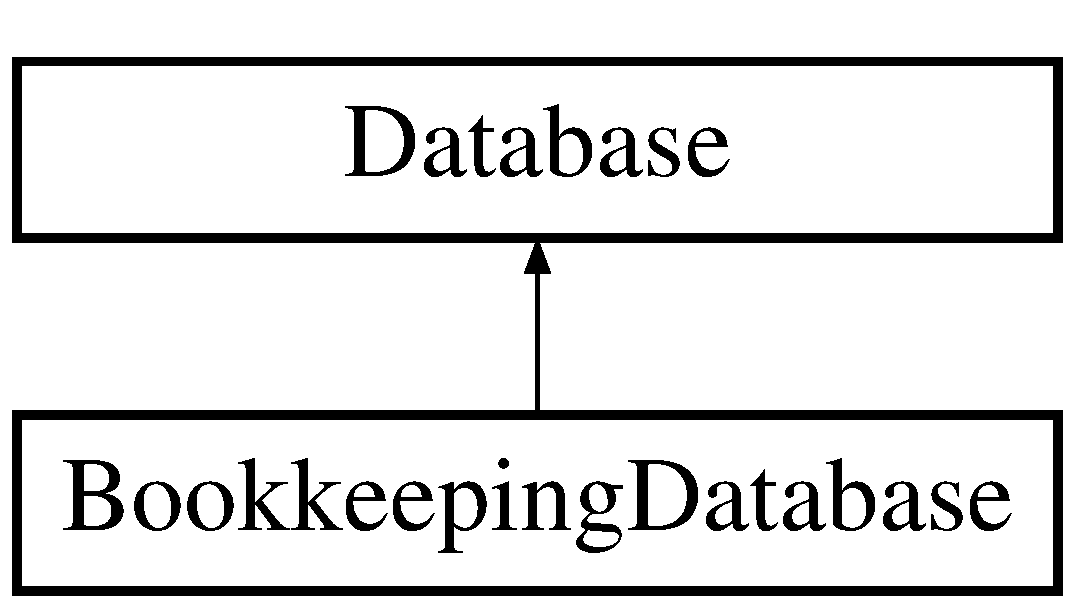
\includegraphics[height=2.000000cm]{class_bookkeeping_database}
\end{center}
\end{figure}
\subsection*{Public Member Functions}
\begin{DoxyCompactItemize}
\item 
\hyperlink{class_bookkeeping_database_a1a74efb5f220809bb0e058b6d0140390}{Bookkeeping\+Database} ()
\item 
\hyperlink{class_bookkeeping_database_a90eea3eca364a7bee4de3bc4ce99061d}{$\sim$\+Bookkeeping\+Database} ()
\item 
void \hyperlink{class_bookkeeping_database_a16c4a4334e3c093df2e158f82bbbd09c}{insert\+Task\+Data} (string data)
\item 
void \hyperlink{class_bookkeeping_database_acce0f8743a2943476172fe5b3e2626e3}{create\+File} ()
\end{DoxyCompactItemize}


\subsection{Detailed Description}


Definition at line 14 of file Bookkeeping\+Database.\+h.



\subsection{Constructor \& Destructor Documentation}
\hypertarget{class_bookkeeping_database_a1a74efb5f220809bb0e058b6d0140390}{}\index{Bookkeeping\+Database@{Bookkeeping\+Database}!Bookkeeping\+Database@{Bookkeeping\+Database}}
\index{Bookkeeping\+Database@{Bookkeeping\+Database}!Bookkeeping\+Database@{Bookkeeping\+Database}}
\subsubsection[{Bookkeeping\+Database}]{\setlength{\rightskip}{0pt plus 5cm}Bookkeeping\+Database\+::\+Bookkeeping\+Database (
\begin{DoxyParamCaption}
{}
\end{DoxyParamCaption}
)}\label{class_bookkeeping_database_a1a74efb5f220809bb0e058b6d0140390}


Definition at line 20 of file Bookkeeping\+Database.\+cpp.

\hypertarget{class_bookkeeping_database_a90eea3eca364a7bee4de3bc4ce99061d}{}\index{Bookkeeping\+Database@{Bookkeeping\+Database}!````~Bookkeeping\+Database@{$\sim$\+Bookkeeping\+Database}}
\index{````~Bookkeeping\+Database@{$\sim$\+Bookkeeping\+Database}!Bookkeeping\+Database@{Bookkeeping\+Database}}
\subsubsection[{$\sim$\+Bookkeeping\+Database}]{\setlength{\rightskip}{0pt plus 5cm}Bookkeeping\+Database\+::$\sim$\+Bookkeeping\+Database (
\begin{DoxyParamCaption}
{}
\end{DoxyParamCaption}
)}\label{class_bookkeeping_database_a90eea3eca364a7bee4de3bc4ce99061d}


Definition at line 25 of file Bookkeeping\+Database.\+cpp.



\subsection{Member Function Documentation}
\hypertarget{class_bookkeeping_database_acce0f8743a2943476172fe5b3e2626e3}{}\index{Bookkeeping\+Database@{Bookkeeping\+Database}!create\+File@{create\+File}}
\index{create\+File@{create\+File}!Bookkeeping\+Database@{Bookkeeping\+Database}}
\subsubsection[{create\+File}]{\setlength{\rightskip}{0pt plus 5cm}void Bookkeeping\+Database\+::create\+File (
\begin{DoxyParamCaption}
{}
\end{DoxyParamCaption}
)}\label{class_bookkeeping_database_acce0f8743a2943476172fe5b3e2626e3}


Definition at line 45 of file Bookkeeping\+Database.\+cpp.

\hypertarget{class_bookkeeping_database_a16c4a4334e3c093df2e158f82bbbd09c}{}\index{Bookkeeping\+Database@{Bookkeeping\+Database}!insert\+Task\+Data@{insert\+Task\+Data}}
\index{insert\+Task\+Data@{insert\+Task\+Data}!Bookkeeping\+Database@{Bookkeeping\+Database}}
\subsubsection[{insert\+Task\+Data}]{\setlength{\rightskip}{0pt plus 5cm}void Bookkeeping\+Database\+::insert\+Task\+Data (
\begin{DoxyParamCaption}
\item[{string}]{data}
\end{DoxyParamCaption}
)\hspace{0.3cm}{\ttfamily [virtual]}}\label{class_bookkeeping_database_a16c4a4334e3c093df2e158f82bbbd09c}


Implements \hyperlink{class_database_aa80c3dd72d5b120a148ef31ccc7430b6}{Database}.



Definition at line 50 of file Bookkeeping\+Database.\+cpp.



The documentation for this class was generated from the following files\+:\begin{DoxyCompactItemize}
\item 
src/database/\hyperlink{_bookkeeping_database_8h}{Bookkeeping\+Database.\+h}\item 
src/database/\hyperlink{_bookkeeping_database_8cpp}{Bookkeeping\+Database.\+cpp}\end{DoxyCompactItemize}

\hypertarget{classel_1_1_callback}{}\section{el\+:\+:Callback$<$ T $>$ Class Template Reference}
\label{classel_1_1_callback}\index{el\+::\+Callback$<$ T $>$@{el\+::\+Callback$<$ T $>$}}


{\ttfamily \#include $<$easylogging++.\+h$>$}

Inheritance diagram for el\+:\+:Callback$<$ T $>$\+:\begin{figure}[H]
\begin{center}
\leavevmode
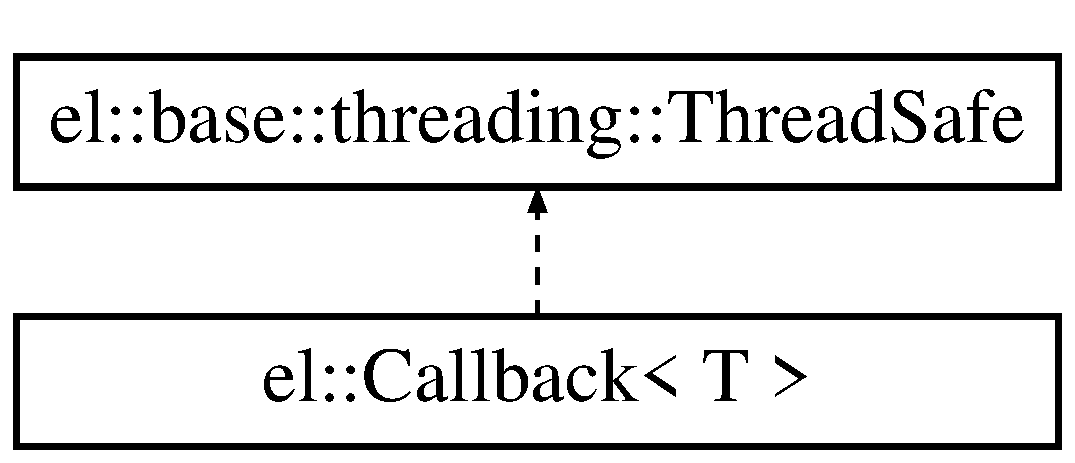
\includegraphics[height=2.000000cm]{classel_1_1_callback}
\end{center}
\end{figure}
\subsection*{Public Member Functions}
\begin{DoxyCompactItemize}
\item 
\hyperlink{classel_1_1_callback_a58b0b0516f68247681a6a5da21a9d953}{Callback} (void)
\item 
bool \hyperlink{classel_1_1_callback_a1e3089fd19a11965e7b98bd423116bbd}{enabled} (void) const 
\item 
void \hyperlink{classel_1_1_callback_a05e68cb0b5ea4423913fa2ec4ea306b4}{set\+Enabled} (bool \hyperlink{classel_1_1_callback_a1e3089fd19a11965e7b98bd423116bbd}{enabled})
\end{DoxyCompactItemize}
\subsection*{Protected Member Functions}
\begin{DoxyCompactItemize}
\item 
virtual void \hyperlink{classel_1_1_callback_a8997c7971d65062c374ef24e653061be}{handle} (const T $\ast$handle\+Ptr)=0
\end{DoxyCompactItemize}


\subsection{Detailed Description}
\subsubsection*{template$<$typename T$>$class el\+::\+Callback$<$ T $>$}



Definition at line 409 of file easylogging++.\+h.



\subsection{Constructor \& Destructor Documentation}
\hypertarget{classel_1_1_callback_a58b0b0516f68247681a6a5da21a9d953}{}\index{el\+::\+Callback@{el\+::\+Callback}!Callback@{Callback}}
\index{Callback@{Callback}!el\+::\+Callback@{el\+::\+Callback}}
\subsubsection[{Callback}]{\setlength{\rightskip}{0pt plus 5cm}template$<$typename T$>$ {\bf el\+::\+Callback}$<$ T $>$\+::{\bf Callback} (
\begin{DoxyParamCaption}
\item[{void}]{}
\end{DoxyParamCaption}
)\hspace{0.3cm}{\ttfamily [inline]}}\label{classel_1_1_callback_a58b0b0516f68247681a6a5da21a9d953}


Definition at line 3323 of file easylogging++.\+h.



\subsection{Member Function Documentation}
\hypertarget{classel_1_1_callback_a1e3089fd19a11965e7b98bd423116bbd}{}\index{el\+::\+Callback@{el\+::\+Callback}!enabled@{enabled}}
\index{enabled@{enabled}!el\+::\+Callback@{el\+::\+Callback}}
\subsubsection[{enabled}]{\setlength{\rightskip}{0pt plus 5cm}template$<$typename T$>$ bool {\bf el\+::\+Callback}$<$ T $>$\+::enabled (
\begin{DoxyParamCaption}
\item[{void}]{}
\end{DoxyParamCaption}
) const\hspace{0.3cm}{\ttfamily [inline]}}\label{classel_1_1_callback_a1e3089fd19a11965e7b98bd423116bbd}


Definition at line 3324 of file easylogging++.\+h.

\hypertarget{classel_1_1_callback_a8997c7971d65062c374ef24e653061be}{}\index{el\+::\+Callback@{el\+::\+Callback}!handle@{handle}}
\index{handle@{handle}!el\+::\+Callback@{el\+::\+Callback}}
\subsubsection[{handle}]{\setlength{\rightskip}{0pt plus 5cm}template$<$typename T$>$ virtual void {\bf el\+::\+Callback}$<$ T $>$\+::handle (
\begin{DoxyParamCaption}
\item[{const T $\ast$}]{handle\+Ptr}
\end{DoxyParamCaption}
)\hspace{0.3cm}{\ttfamily [protected]}, {\ttfamily [pure virtual]}}\label{classel_1_1_callback_a8997c7971d65062c374ef24e653061be}


Implemented in \hyperlink{classel_1_1base_1_1_default_performance_tracking_callback_afabb8820e1bd9a7fb89508fe11f59d37}{el\+::base\+::\+Default\+Performance\+Tracking\+Callback}, and \hyperlink{classel_1_1base_1_1_default_log_dispatch_callback_acdac30f202c245500e6d94c55eee6d95}{el\+::base\+::\+Default\+Log\+Dispatch\+Callback}.

\hypertarget{classel_1_1_callback_a05e68cb0b5ea4423913fa2ec4ea306b4}{}\index{el\+::\+Callback@{el\+::\+Callback}!set\+Enabled@{set\+Enabled}}
\index{set\+Enabled@{set\+Enabled}!el\+::\+Callback@{el\+::\+Callback}}
\subsubsection[{set\+Enabled}]{\setlength{\rightskip}{0pt plus 5cm}template$<$typename T$>$ void {\bf el\+::\+Callback}$<$ T $>$\+::set\+Enabled (
\begin{DoxyParamCaption}
\item[{bool}]{enabled}
\end{DoxyParamCaption}
)\hspace{0.3cm}{\ttfamily [inline]}}\label{classel_1_1_callback_a05e68cb0b5ea4423913fa2ec4ea306b4}


Definition at line 3325 of file easylogging++.\+h.



The documentation for this class was generated from the following file\+:\begin{DoxyCompactItemize}
\item 
lib/\hyperlink{easylogging_09_09_8h}{easylogging++.\+h}\end{DoxyCompactItemize}

\hypertarget{classel_1_1base_1_1utils_1_1_command_line_args}{}\section{el\+:\+:base\+:\+:utils\+:\+:Command\+Line\+Args Class Reference}
\label{classel_1_1base_1_1utils_1_1_command_line_args}\index{el\+::base\+::utils\+::\+Command\+Line\+Args@{el\+::base\+::utils\+::\+Command\+Line\+Args}}


Command line arguments for application if specified using \hyperlink{classel_1_1_helpers_a68748f618a0c2840b96dc12532b09bf0}{el\+::\+Helpers\+::set\+Args}(..) or S\+T\+A\+R\+T\+\_\+\+E\+A\+S\+Y\+L\+O\+G\+G\+I\+N\+G\+P\+P(..)  




{\ttfamily \#include $<$easylogging++.\+h$>$}

\subsection*{Public Member Functions}
\begin{DoxyCompactItemize}
\item 
\hyperlink{classel_1_1base_1_1utils_1_1_command_line_args_a58a5e0acd54a1412d09ec39a1140f067}{Command\+Line\+Args} (void)
\item 
\hyperlink{classel_1_1base_1_1utils_1_1_command_line_args_a9872b14450e9cd1c1bd96227743c083b}{Command\+Line\+Args} (int argc, const char $\ast$$\ast$argv)
\item 
\hyperlink{classel_1_1base_1_1utils_1_1_command_line_args_a297b31b31829d9545d6e808f4be9195c}{Command\+Line\+Args} (int argc, char $\ast$$\ast$argv)
\item 
virtual \hyperlink{classel_1_1base_1_1utils_1_1_command_line_args_a41c4aafeffaef7ab6320feb709d6a0d6}{$\sim$\+Command\+Line\+Args} (void)
\item 
void \hyperlink{classel_1_1base_1_1utils_1_1_command_line_args_a2d59b4184e0a6a314ef1c9a4c6d946e6}{set\+Args} (int argc, const char $\ast$$\ast$argv)
\begin{DoxyCompactList}\small\item\em Sets arguments and parses them. \end{DoxyCompactList}\item 
void \hyperlink{classel_1_1base_1_1utils_1_1_command_line_args_af88a16e6ce7b5d48f9679f304367b27a}{set\+Args} (int argc, char $\ast$$\ast$argv)
\begin{DoxyCompactList}\small\item\em Sets arguments and parses them. \end{DoxyCompactList}\item 
bool \hyperlink{classel_1_1base_1_1utils_1_1_command_line_args_acc9fa8eeed2deecffb6019173de5ab48}{has\+Param\+With\+Value} (const char $\ast$param\+Key) const 
\begin{DoxyCompactList}\small\item\em Returns true if arguments contain param\+Key with a value (seperated by \textquotesingle{}=\textquotesingle{}) \end{DoxyCompactList}\item 
const char $\ast$ \hyperlink{classel_1_1base_1_1utils_1_1_command_line_args_ad1abe08dfdbdd95c72474197ba4a3cbd}{get\+Param\+Value} (const char $\ast$param\+Key) const 
\begin{DoxyCompactList}\small\item\em Returns value of arguments. \end{DoxyCompactList}\item 
bool \hyperlink{classel_1_1base_1_1utils_1_1_command_line_args_a83fbd7e5d8422e98a7d58d65283f144f}{has\+Param} (const char $\ast$param\+Key) const 
\begin{DoxyCompactList}\small\item\em Return true if arguments has a param (not having a value) i,e without \textquotesingle{}=\textquotesingle{}. \end{DoxyCompactList}\item 
bool \hyperlink{classel_1_1base_1_1utils_1_1_command_line_args_a014c586d14eb73f2ec1deb5b08bdd6a7}{empty} (void) const 
\begin{DoxyCompactList}\small\item\em Returns true if no params available. This exclude argv\mbox{[}0\mbox{]}. \end{DoxyCompactList}\item 
std\+::size\+\_\+t \hyperlink{classel_1_1base_1_1utils_1_1_command_line_args_ab335b66a2ca2dea6c9c7b8d54760e975}{size} (void) const 
\begin{DoxyCompactList}\small\item\em Returns total number of arguments. This exclude argv\mbox{[}0\mbox{]}. \end{DoxyCompactList}\end{DoxyCompactItemize}
\subsection*{Friends}
\begin{DoxyCompactItemize}
\item 
\hyperlink{namespaceel_1_1base_1_1type_a74ea109bf34d1c44926837fb0830f445}{base\+::type\+::ostream\+\_\+t} \& \hyperlink{classel_1_1base_1_1utils_1_1_command_line_args_aee5ba4c037136cd1d54026dd75927b10}{operator$<$$<$} (\hyperlink{namespaceel_1_1base_1_1type_a74ea109bf34d1c44926837fb0830f445}{base\+::type\+::ostream\+\_\+t} \&os, const \hyperlink{classel_1_1base_1_1utils_1_1_command_line_args}{Command\+Line\+Args} \&c)
\end{DoxyCompactItemize}


\subsection{Detailed Description}
Command line arguments for application if specified using \hyperlink{classel_1_1_helpers_a68748f618a0c2840b96dc12532b09bf0}{el\+::\+Helpers\+::set\+Args}(..) or S\+T\+A\+R\+T\+\_\+\+E\+A\+S\+Y\+L\+O\+G\+G\+I\+N\+G\+P\+P(..) 

Definition at line 1724 of file easylogging++.\+h.



\subsection{Constructor \& Destructor Documentation}
\hypertarget{classel_1_1base_1_1utils_1_1_command_line_args_a58a5e0acd54a1412d09ec39a1140f067}{}\index{el\+::base\+::utils\+::\+Command\+Line\+Args@{el\+::base\+::utils\+::\+Command\+Line\+Args}!Command\+Line\+Args@{Command\+Line\+Args}}
\index{Command\+Line\+Args@{Command\+Line\+Args}!el\+::base\+::utils\+::\+Command\+Line\+Args@{el\+::base\+::utils\+::\+Command\+Line\+Args}}
\subsubsection[{Command\+Line\+Args}]{\setlength{\rightskip}{0pt plus 5cm}el\+::base\+::utils\+::\+Command\+Line\+Args\+::\+Command\+Line\+Args (
\begin{DoxyParamCaption}
\item[{void}]{}
\end{DoxyParamCaption}
)\hspace{0.3cm}{\ttfamily [inline]}}\label{classel_1_1base_1_1utils_1_1_command_line_args_a58a5e0acd54a1412d09ec39a1140f067}


Definition at line 1726 of file easylogging++.\+h.

\hypertarget{classel_1_1base_1_1utils_1_1_command_line_args_a9872b14450e9cd1c1bd96227743c083b}{}\index{el\+::base\+::utils\+::\+Command\+Line\+Args@{el\+::base\+::utils\+::\+Command\+Line\+Args}!Command\+Line\+Args@{Command\+Line\+Args}}
\index{Command\+Line\+Args@{Command\+Line\+Args}!el\+::base\+::utils\+::\+Command\+Line\+Args@{el\+::base\+::utils\+::\+Command\+Line\+Args}}
\subsubsection[{Command\+Line\+Args}]{\setlength{\rightskip}{0pt plus 5cm}el\+::base\+::utils\+::\+Command\+Line\+Args\+::\+Command\+Line\+Args (
\begin{DoxyParamCaption}
\item[{int}]{argc, }
\item[{const char $\ast$$\ast$}]{argv}
\end{DoxyParamCaption}
)\hspace{0.3cm}{\ttfamily [inline]}}\label{classel_1_1base_1_1utils_1_1_command_line_args_a9872b14450e9cd1c1bd96227743c083b}


Definition at line 1729 of file easylogging++.\+h.

\hypertarget{classel_1_1base_1_1utils_1_1_command_line_args_a297b31b31829d9545d6e808f4be9195c}{}\index{el\+::base\+::utils\+::\+Command\+Line\+Args@{el\+::base\+::utils\+::\+Command\+Line\+Args}!Command\+Line\+Args@{Command\+Line\+Args}}
\index{Command\+Line\+Args@{Command\+Line\+Args}!el\+::base\+::utils\+::\+Command\+Line\+Args@{el\+::base\+::utils\+::\+Command\+Line\+Args}}
\subsubsection[{Command\+Line\+Args}]{\setlength{\rightskip}{0pt plus 5cm}el\+::base\+::utils\+::\+Command\+Line\+Args\+::\+Command\+Line\+Args (
\begin{DoxyParamCaption}
\item[{int}]{argc, }
\item[{char $\ast$$\ast$}]{argv}
\end{DoxyParamCaption}
)\hspace{0.3cm}{\ttfamily [inline]}}\label{classel_1_1base_1_1utils_1_1_command_line_args_a297b31b31829d9545d6e808f4be9195c}


Definition at line 1732 of file easylogging++.\+h.

\hypertarget{classel_1_1base_1_1utils_1_1_command_line_args_a41c4aafeffaef7ab6320feb709d6a0d6}{}\index{el\+::base\+::utils\+::\+Command\+Line\+Args@{el\+::base\+::utils\+::\+Command\+Line\+Args}!````~Command\+Line\+Args@{$\sim$\+Command\+Line\+Args}}
\index{````~Command\+Line\+Args@{$\sim$\+Command\+Line\+Args}!el\+::base\+::utils\+::\+Command\+Line\+Args@{el\+::base\+::utils\+::\+Command\+Line\+Args}}
\subsubsection[{$\sim$\+Command\+Line\+Args}]{\setlength{\rightskip}{0pt plus 5cm}virtual el\+::base\+::utils\+::\+Command\+Line\+Args\+::$\sim$\+Command\+Line\+Args (
\begin{DoxyParamCaption}
\item[{void}]{}
\end{DoxyParamCaption}
)\hspace{0.3cm}{\ttfamily [inline]}, {\ttfamily [virtual]}}\label{classel_1_1base_1_1utils_1_1_command_line_args_a41c4aafeffaef7ab6320feb709d6a0d6}


Definition at line 1735 of file easylogging++.\+h.



\subsection{Member Function Documentation}
\hypertarget{classel_1_1base_1_1utils_1_1_command_line_args_a014c586d14eb73f2ec1deb5b08bdd6a7}{}\index{el\+::base\+::utils\+::\+Command\+Line\+Args@{el\+::base\+::utils\+::\+Command\+Line\+Args}!empty@{empty}}
\index{empty@{empty}!el\+::base\+::utils\+::\+Command\+Line\+Args@{el\+::base\+::utils\+::\+Command\+Line\+Args}}
\subsubsection[{empty}]{\setlength{\rightskip}{0pt plus 5cm}bool el\+::base\+::utils\+::\+Command\+Line\+Args\+::empty (
\begin{DoxyParamCaption}
\item[{void}]{}
\end{DoxyParamCaption}
) const\hspace{0.3cm}{\ttfamily [inline]}}\label{classel_1_1base_1_1utils_1_1_command_line_args_a014c586d14eb73f2ec1deb5b08bdd6a7}


Returns true if no params available. This exclude argv\mbox{[}0\mbox{]}. 



Definition at line 1784 of file easylogging++.\+h.

\hypertarget{classel_1_1base_1_1utils_1_1_command_line_args_ad1abe08dfdbdd95c72474197ba4a3cbd}{}\index{el\+::base\+::utils\+::\+Command\+Line\+Args@{el\+::base\+::utils\+::\+Command\+Line\+Args}!get\+Param\+Value@{get\+Param\+Value}}
\index{get\+Param\+Value@{get\+Param\+Value}!el\+::base\+::utils\+::\+Command\+Line\+Args@{el\+::base\+::utils\+::\+Command\+Line\+Args}}
\subsubsection[{get\+Param\+Value}]{\setlength{\rightskip}{0pt plus 5cm}const char$\ast$ el\+::base\+::utils\+::\+Command\+Line\+Args\+::get\+Param\+Value (
\begin{DoxyParamCaption}
\item[{const char $\ast$}]{param\+Key}
\end{DoxyParamCaption}
) const\hspace{0.3cm}{\ttfamily [inline]}}\label{classel_1_1base_1_1utils_1_1_command_line_args_ad1abe08dfdbdd95c72474197ba4a3cbd}


Returns value of arguments. 

\begin{DoxySeeAlso}{See also}
has\+Param\+With\+Value(const char$\ast$) 
\end{DoxySeeAlso}


Definition at line 1776 of file easylogging++.\+h.

\hypertarget{classel_1_1base_1_1utils_1_1_command_line_args_a83fbd7e5d8422e98a7d58d65283f144f}{}\index{el\+::base\+::utils\+::\+Command\+Line\+Args@{el\+::base\+::utils\+::\+Command\+Line\+Args}!has\+Param@{has\+Param}}
\index{has\+Param@{has\+Param}!el\+::base\+::utils\+::\+Command\+Line\+Args@{el\+::base\+::utils\+::\+Command\+Line\+Args}}
\subsubsection[{has\+Param}]{\setlength{\rightskip}{0pt plus 5cm}bool el\+::base\+::utils\+::\+Command\+Line\+Args\+::has\+Param (
\begin{DoxyParamCaption}
\item[{const char $\ast$}]{param\+Key}
\end{DoxyParamCaption}
) const\hspace{0.3cm}{\ttfamily [inline]}}\label{classel_1_1base_1_1utils_1_1_command_line_args_a83fbd7e5d8422e98a7d58d65283f144f}


Return true if arguments has a param (not having a value) i,e without \textquotesingle{}=\textquotesingle{}. 



Definition at line 1780 of file easylogging++.\+h.

\hypertarget{classel_1_1base_1_1utils_1_1_command_line_args_acc9fa8eeed2deecffb6019173de5ab48}{}\index{el\+::base\+::utils\+::\+Command\+Line\+Args@{el\+::base\+::utils\+::\+Command\+Line\+Args}!has\+Param\+With\+Value@{has\+Param\+With\+Value}}
\index{has\+Param\+With\+Value@{has\+Param\+With\+Value}!el\+::base\+::utils\+::\+Command\+Line\+Args@{el\+::base\+::utils\+::\+Command\+Line\+Args}}
\subsubsection[{has\+Param\+With\+Value}]{\setlength{\rightskip}{0pt plus 5cm}bool el\+::base\+::utils\+::\+Command\+Line\+Args\+::has\+Param\+With\+Value (
\begin{DoxyParamCaption}
\item[{const char $\ast$}]{param\+Key}
\end{DoxyParamCaption}
) const\hspace{0.3cm}{\ttfamily [inline]}}\label{classel_1_1base_1_1utils_1_1_command_line_args_acc9fa8eeed2deecffb6019173de5ab48}


Returns true if arguments contain param\+Key with a value (seperated by \textquotesingle{}=\textquotesingle{}) 



Definition at line 1771 of file easylogging++.\+h.

\hypertarget{classel_1_1base_1_1utils_1_1_command_line_args_a2d59b4184e0a6a314ef1c9a4c6d946e6}{}\index{el\+::base\+::utils\+::\+Command\+Line\+Args@{el\+::base\+::utils\+::\+Command\+Line\+Args}!set\+Args@{set\+Args}}
\index{set\+Args@{set\+Args}!el\+::base\+::utils\+::\+Command\+Line\+Args@{el\+::base\+::utils\+::\+Command\+Line\+Args}}
\subsubsection[{set\+Args}]{\setlength{\rightskip}{0pt plus 5cm}void el\+::base\+::utils\+::\+Command\+Line\+Args\+::set\+Args (
\begin{DoxyParamCaption}
\item[{int}]{argc, }
\item[{const char $\ast$$\ast$}]{argv}
\end{DoxyParamCaption}
)\hspace{0.3cm}{\ttfamily [inline]}}\label{classel_1_1base_1_1utils_1_1_command_line_args_a2d59b4184e0a6a314ef1c9a4c6d946e6}


Sets arguments and parses them. 



Definition at line 1737 of file easylogging++.\+h.

\hypertarget{classel_1_1base_1_1utils_1_1_command_line_args_af88a16e6ce7b5d48f9679f304367b27a}{}\index{el\+::base\+::utils\+::\+Command\+Line\+Args@{el\+::base\+::utils\+::\+Command\+Line\+Args}!set\+Args@{set\+Args}}
\index{set\+Args@{set\+Args}!el\+::base\+::utils\+::\+Command\+Line\+Args@{el\+::base\+::utils\+::\+Command\+Line\+Args}}
\subsubsection[{set\+Args}]{\setlength{\rightskip}{0pt plus 5cm}void el\+::base\+::utils\+::\+Command\+Line\+Args\+::set\+Args (
\begin{DoxyParamCaption}
\item[{int}]{argc, }
\item[{char $\ast$$\ast$}]{argv}
\end{DoxyParamCaption}
)\hspace{0.3cm}{\ttfamily [inline]}}\label{classel_1_1base_1_1utils_1_1_command_line_args_af88a16e6ce7b5d48f9679f304367b27a}


Sets arguments and parses them. 



Definition at line 1741 of file easylogging++.\+h.

\hypertarget{classel_1_1base_1_1utils_1_1_command_line_args_ab335b66a2ca2dea6c9c7b8d54760e975}{}\index{el\+::base\+::utils\+::\+Command\+Line\+Args@{el\+::base\+::utils\+::\+Command\+Line\+Args}!size@{size}}
\index{size@{size}!el\+::base\+::utils\+::\+Command\+Line\+Args@{el\+::base\+::utils\+::\+Command\+Line\+Args}}
\subsubsection[{size}]{\setlength{\rightskip}{0pt plus 5cm}std\+::size\+\_\+t el\+::base\+::utils\+::\+Command\+Line\+Args\+::size (
\begin{DoxyParamCaption}
\item[{void}]{}
\end{DoxyParamCaption}
) const\hspace{0.3cm}{\ttfamily [inline]}}\label{classel_1_1base_1_1utils_1_1_command_line_args_ab335b66a2ca2dea6c9c7b8d54760e975}


Returns total number of arguments. This exclude argv\mbox{[}0\mbox{]}. 



Definition at line 1788 of file easylogging++.\+h.



\subsection{Friends And Related Function Documentation}
\hypertarget{classel_1_1base_1_1utils_1_1_command_line_args_aee5ba4c037136cd1d54026dd75927b10}{}\index{el\+::base\+::utils\+::\+Command\+Line\+Args@{el\+::base\+::utils\+::\+Command\+Line\+Args}!operator$<$$<$@{operator$<$$<$}}
\index{operator$<$$<$@{operator$<$$<$}!el\+::base\+::utils\+::\+Command\+Line\+Args@{el\+::base\+::utils\+::\+Command\+Line\+Args}}
\subsubsection[{operator$<$$<$}]{\setlength{\rightskip}{0pt plus 5cm}{\bf base\+::type\+::ostream\+\_\+t}\& operator$<$$<$ (
\begin{DoxyParamCaption}
\item[{{\bf base\+::type\+::ostream\+\_\+t} \&}]{os, }
\item[{const {\bf Command\+Line\+Args} \&}]{c}
\end{DoxyParamCaption}
)\hspace{0.3cm}{\ttfamily [friend]}}\label{classel_1_1base_1_1utils_1_1_command_line_args_aee5ba4c037136cd1d54026dd75927b10}


Definition at line 1791 of file easylogging++.\+h.



The documentation for this class was generated from the following file\+:\begin{DoxyCompactItemize}
\item 
lib/\hyperlink{easylogging_09_09_8h}{easylogging++.\+h}\end{DoxyCompactItemize}

\hypertarget{class_command_line_parser}{}\section{Command\+Line\+Parser Class Reference}
\label{class_command_line_parser}\index{Command\+Line\+Parser@{Command\+Line\+Parser}}


{\ttfamily \#include $<$Command\+Line\+Parser.\+h$>$}

\subsection*{Public Member Functions}
\begin{DoxyCompactItemize}
\item 
void \hyperlink{class_command_line_parser_a90a8555f0902b43fcea52671f9c98883}{parse} (int argc, char $\ast$argv\mbox{[}$\,$\mbox{]})
\item 
\hyperlink{_design_enum_8h_aefcba5d81ba393e442410d16ebe78ac7}{Design\+Enum} \hyperlink{class_command_line_parser_a8399461d8c096889f5d37045b5935921}{get\+\_\+design} ()
\item 
\hyperlink{_strategy_enum_8h_aa770fe6711c27326278b9e4ab326cd10}{Strategy\+Enum} \hyperlink{class_command_line_parser_a55e3200ff40b200cebfeb4dc645319df}{get\+\_\+strategy} ()
\end{DoxyCompactItemize}


\subsection{Detailed Description}
The command line parser search in the given command line parameters to find scheduler specific ons and parse them. The given parameters are not manipulated and can be passed to the scientific code.

\begin{DoxyAuthor}{Author}
Fabio Broghammer 
\end{DoxyAuthor}
\begin{DoxyVersion}{Version}
1.\+0 
\end{DoxyVersion}


Definition at line 15 of file Command\+Line\+Parser.\+h.



\subsection{Member Function Documentation}
\hypertarget{class_command_line_parser_a8399461d8c096889f5d37045b5935921}{}\index{Command\+Line\+Parser@{Command\+Line\+Parser}!get\+\_\+design@{get\+\_\+design}}
\index{get\+\_\+design@{get\+\_\+design}!Command\+Line\+Parser@{Command\+Line\+Parser}}
\subsubsection[{get\+\_\+design}]{\setlength{\rightskip}{0pt plus 5cm}{\bf Design\+Enum} Command\+Line\+Parser\+::get\+\_\+design (
\begin{DoxyParamCaption}
{}
\end{DoxyParamCaption}
)}\label{class_command_line_parser_a8399461d8c096889f5d37045b5935921}
Returns the design.

\begin{DoxyReturn}{Returns}
the design 
\end{DoxyReturn}


Definition at line 9 of file Command\+Line\+Parser.\+cpp.

\hypertarget{class_command_line_parser_a55e3200ff40b200cebfeb4dc645319df}{}\index{Command\+Line\+Parser@{Command\+Line\+Parser}!get\+\_\+strategy@{get\+\_\+strategy}}
\index{get\+\_\+strategy@{get\+\_\+strategy}!Command\+Line\+Parser@{Command\+Line\+Parser}}
\subsubsection[{get\+\_\+strategy}]{\setlength{\rightskip}{0pt plus 5cm}{\bf Strategy\+Enum} Command\+Line\+Parser\+::get\+\_\+strategy (
\begin{DoxyParamCaption}
{}
\end{DoxyParamCaption}
)}\label{class_command_line_parser_a55e3200ff40b200cebfeb4dc645319df}
Returns the strategy.

\begin{DoxyReturn}{Returns}
the strategy 
\end{DoxyReturn}


Definition at line 14 of file Command\+Line\+Parser.\+cpp.

\hypertarget{class_command_line_parser_a90a8555f0902b43fcea52671f9c98883}{}\index{Command\+Line\+Parser@{Command\+Line\+Parser}!parse@{parse}}
\index{parse@{parse}!Command\+Line\+Parser@{Command\+Line\+Parser}}
\subsubsection[{parse}]{\setlength{\rightskip}{0pt plus 5cm}void Command\+Line\+Parser\+::parse (
\begin{DoxyParamCaption}
\item[{int}]{argc, }
\item[{char $\ast$}]{argv\mbox{[}$\,$\mbox{]}}
\end{DoxyParamCaption}
)}\label{class_command_line_parser_a90a8555f0902b43fcea52671f9c98883}
Parse the given command line parameter and search scheduler specific one.


\begin{DoxyParams}{Parameters}
{\em argc} & command line parameter count \\
\hline
{\em argv} & command line parameter \\
\hline
\end{DoxyParams}


Definition at line 19 of file Command\+Line\+Parser.\+cpp.



The documentation for this class was generated from the following files\+:\begin{DoxyCompactItemize}
\item 
src/util/\hyperlink{_command_line_parser_8h}{Command\+Line\+Parser.\+h}\item 
src/util/\hyperlink{_command_line_parser_8cpp}{Command\+Line\+Parser.\+cpp}\end{DoxyCompactItemize}

\hypertarget{class_comparison_class_l_j_f}{}\section{Comparison\+Class\+L\+J\+F Class Reference}
\label{class_comparison_class_l_j_f}\index{Comparison\+Class\+L\+J\+F@{Comparison\+Class\+L\+J\+F}}


{\ttfamily \#include $<$L\+J\+F.\+h$>$}

\subsection*{Public Member Functions}
\begin{DoxyCompactItemize}
\item 
bool \hyperlink{class_comparison_class_l_j_f_a0e49bbee2ff869b1b2b31ad9e9a863d0}{operator()} (\hyperlink{_scheduling_strategy_8h_a3fb457f0594d33676e56256c3403e52b}{Task\+Time\+Type} task\+\_\+time\+\_\+1, \hyperlink{_scheduling_strategy_8h_a3fb457f0594d33676e56256c3403e52b}{Task\+Time\+Type} task\+\_\+time\+\_\+2)
\end{DoxyCompactItemize}


\subsection{Detailed Description}
This class is a custom comparison class for the std\+::priority\+\_\+queue. This class is used to order the priority queue. This class is used from the \hyperlink{class_l_j_f}{L\+J\+F} class.

\begin{DoxyAuthor}{Author}
Fabio Broghammer 
\end{DoxyAuthor}
\begin{DoxyVersion}{Version}
1.\+0 
\end{DoxyVersion}


Definition at line 14 of file L\+J\+F.\+h.



\subsection{Member Function Documentation}
\hypertarget{class_comparison_class_l_j_f_a0e49bbee2ff869b1b2b31ad9e9a863d0}{}\index{Comparison\+Class\+L\+J\+F@{Comparison\+Class\+L\+J\+F}!operator()@{operator()}}
\index{operator()@{operator()}!Comparison\+Class\+L\+J\+F@{Comparison\+Class\+L\+J\+F}}
\subsubsection[{operator()}]{\setlength{\rightskip}{0pt plus 5cm}bool Comparison\+Class\+L\+J\+F\+::operator() (
\begin{DoxyParamCaption}
\item[{{\bf Task\+Time\+Type}}]{task\+\_\+time\+\_\+1, }
\item[{{\bf Task\+Time\+Type}}]{task\+\_\+time\+\_\+2}
\end{DoxyParamCaption}
)}\label{class_comparison_class_l_j_f_a0e49bbee2ff869b1b2b31ad9e9a863d0}
Returns true, if the runtime of the task\+\_\+time\+\_\+1 is shorter than the runtime of the task\+\_\+time\+\_\+2. This comparison function is used from the std\+::priority\+\_\+queue to order the tasks.


\begin{DoxyParams}{Parameters}
{\em task\+\_\+time\+\_\+1} & pair of task and runtime to be compared \\
\hline
{\em task\+\_\+time\+\_\+2} & pair of task and runtime to be compared\\
\hline
\end{DoxyParams}
\begin{DoxyReturn}{Returns}
true, if the runtime of the task1 is shorter than the runtime of the task2 
\end{DoxyReturn}


Definition at line 3 of file L\+J\+F.\+cpp.



The documentation for this class was generated from the following files\+:\begin{DoxyCompactItemize}
\item 
src/scheduler/\hyperlink{_l_j_f_8h}{L\+J\+F.\+h}\item 
src/scheduler/\hyperlink{_l_j_f_8cpp}{L\+J\+F.\+cpp}\end{DoxyCompactItemize}

\hypertarget{class_comparison_class_s_j_f}{}\section{Comparison\+Class\+S\+J\+F Class Reference}
\label{class_comparison_class_s_j_f}\index{Comparison\+Class\+S\+J\+F@{Comparison\+Class\+S\+J\+F}}


{\ttfamily \#include $<$S\+J\+F.\+h$>$}

\subsection*{Public Member Functions}
\begin{DoxyCompactItemize}
\item 
bool \hyperlink{class_comparison_class_s_j_f_a7cbc92a9f2f87912040ce92e79d0aa2b}{operator()} (\hyperlink{_scheduling_strategy_8h_a3fb457f0594d33676e56256c3403e52b}{Task\+Time\+Type} task\+\_\+time\+\_\+1, \hyperlink{_scheduling_strategy_8h_a3fb457f0594d33676e56256c3403e52b}{Task\+Time\+Type} task\+\_\+time\+\_\+2)
\end{DoxyCompactItemize}


\subsection{Detailed Description}
This class is a custom comparison class for the std\+::priority\+\_\+queue. This class is used to order the priority queue. This class is used from the \hyperlink{class_s_j_f}{S\+J\+F} class.

\begin{DoxyAuthor}{Author}
Fabio Broghammer 
\end{DoxyAuthor}
\begin{DoxyVersion}{Version}
1.\+0 
\end{DoxyVersion}


Definition at line 14 of file S\+J\+F.\+h.



\subsection{Member Function Documentation}
\hypertarget{class_comparison_class_s_j_f_a7cbc92a9f2f87912040ce92e79d0aa2b}{}\index{Comparison\+Class\+S\+J\+F@{Comparison\+Class\+S\+J\+F}!operator()@{operator()}}
\index{operator()@{operator()}!Comparison\+Class\+S\+J\+F@{Comparison\+Class\+S\+J\+F}}
\subsubsection[{operator()}]{\setlength{\rightskip}{0pt plus 5cm}bool Comparison\+Class\+S\+J\+F\+::operator() (
\begin{DoxyParamCaption}
\item[{{\bf Task\+Time\+Type}}]{task\+\_\+time\+\_\+1, }
\item[{{\bf Task\+Time\+Type}}]{task\+\_\+time\+\_\+2}
\end{DoxyParamCaption}
)}\label{class_comparison_class_s_j_f_a7cbc92a9f2f87912040ce92e79d0aa2b}
Returns true, if the runtime of the task\+\_\+time\+\_\+1 is greater than the runtime of the task\+\_\+time\+\_\+2. This comparison function is used from the std\+::priority\+\_\+queue to order the tasks.


\begin{DoxyParams}{Parameters}
{\em task\+\_\+time\+\_\+1} & pair of task and runtime to be compared \\
\hline
{\em task\+\_\+time\+\_\+2} & pair of task and runtime to be compared\\
\hline
\end{DoxyParams}
\begin{DoxyReturn}{Returns}
true, if the runtime of the task\+\_\+time\+\_\+1 is greater than the runtime of the task\+\_\+time\+\_\+2 
\end{DoxyReturn}


Definition at line 3 of file S\+J\+F.\+cpp.



The documentation for this class was generated from the following files\+:\begin{DoxyCompactItemize}
\item 
src/scheduler/\hyperlink{_s_j_f_8h}{S\+J\+F.\+h}\item 
src/scheduler/\hyperlink{_s_j_f_8cpp}{S\+J\+F.\+cpp}\end{DoxyCompactItemize}

\hypertarget{classel_1_1_configuration}{}\section{el\+:\+:Configuration Class Reference}
\label{classel_1_1_configuration}\index{el\+::\+Configuration@{el\+::\+Configuration}}


Represents single configuration that has representing level, configuration type and a string based value.  




{\ttfamily \#include $<$easylogging++.\+h$>$}

Inheritance diagram for el\+:\+:Configuration\+:\begin{figure}[H]
\begin{center}
\leavevmode
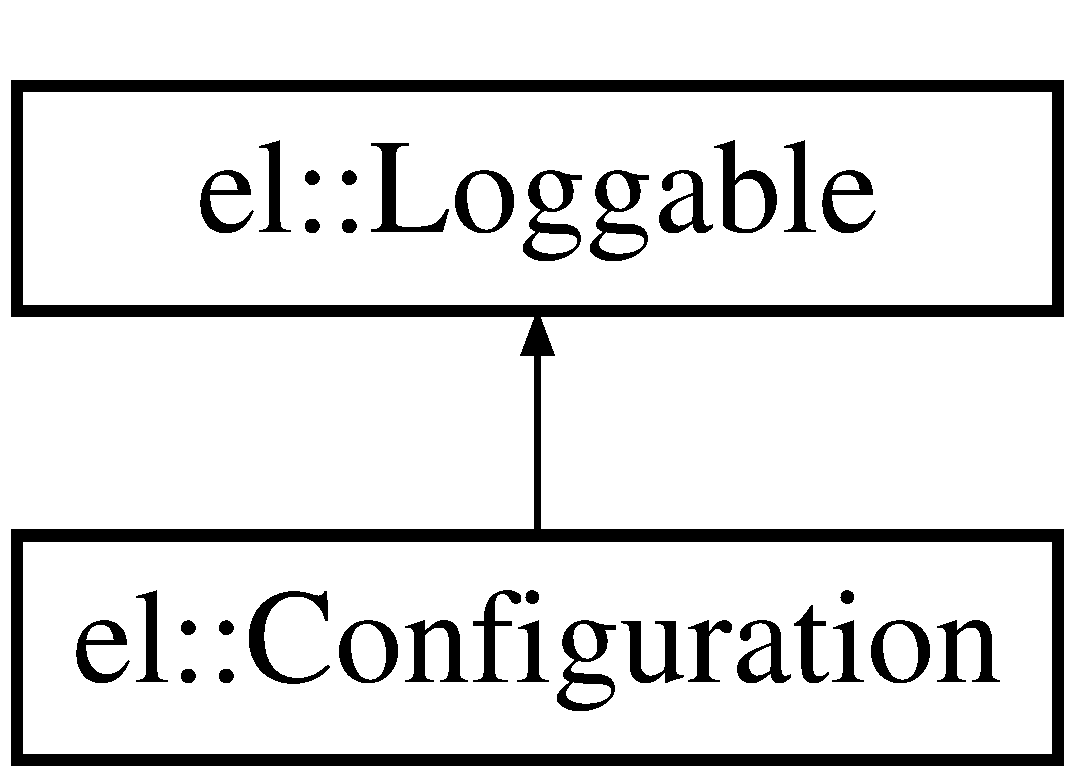
\includegraphics[height=2.000000cm]{classel_1_1_configuration}
\end{center}
\end{figure}
\subsection*{Classes}
\begin{DoxyCompactItemize}
\item 
class \hyperlink{classel_1_1_configuration_1_1_predicate}{Predicate}
\begin{DoxyCompactList}\small\item\em Used to find configuration from configuration (pointers) repository. Avoid using it. \end{DoxyCompactList}\end{DoxyCompactItemize}
\subsection*{Public Member Functions}
\begin{DoxyCompactItemize}
\item 
\hyperlink{classel_1_1_configuration_a71867a89e7d44cac62e0a436f01b484d}{Configuration} (const \hyperlink{classel_1_1_configuration}{Configuration} \&c)
\item 
\hyperlink{classel_1_1_configuration}{Configuration} \& \hyperlink{classel_1_1_configuration_a80bc5b14f61906633cf695ea62e454a2}{operator=} (const \hyperlink{classel_1_1_configuration}{Configuration} \&c)
\item 
virtual \hyperlink{classel_1_1_configuration_abaf0a9e1a96bd40800174982c983a4ac}{$\sim$\+Configuration} (void)
\item 
\hyperlink{classel_1_1_configuration_a1a00abf955e028debaaf7556a647dbf5}{Configuration} (\hyperlink{namespaceel_ab0ac6091262344c52dd2d3ad099e8e36}{Level} \hyperlink{classel_1_1_configuration_a66a96cf46d20204c50718f8a5e3622e2}{level}, \hyperlink{namespaceel_a281f5db6d6163678bc68a8b23b59e124}{Configuration\+Type} \hyperlink{classel_1_1_configuration_aab5091dcca176e309c0a2268ff55db0d}{configuration\+Type}, const std\+::string \&\hyperlink{classel_1_1_configuration_ab31605eb195a222cf32baa4922bb9a3c}{value})
\begin{DoxyCompactList}\small\item\em Full constructor used to sets value of configuration. \end{DoxyCompactList}\item 
\hyperlink{namespaceel_ab0ac6091262344c52dd2d3ad099e8e36}{Level} \hyperlink{classel_1_1_configuration_a66a96cf46d20204c50718f8a5e3622e2}{level} (void) const 
\begin{DoxyCompactList}\small\item\em Gets level of current configuration. \end{DoxyCompactList}\item 
\hyperlink{namespaceel_a281f5db6d6163678bc68a8b23b59e124}{Configuration\+Type} \hyperlink{classel_1_1_configuration_aab5091dcca176e309c0a2268ff55db0d}{configuration\+Type} (void) const 
\begin{DoxyCompactList}\small\item\em Gets configuration type of current configuration. \end{DoxyCompactList}\item 
const std\+::string \& \hyperlink{classel_1_1_configuration_ab31605eb195a222cf32baa4922bb9a3c}{value} (void) const 
\begin{DoxyCompactList}\small\item\em Gets string based configuration value. \end{DoxyCompactList}\item 
void \hyperlink{classel_1_1_configuration_a04755de11422d7570869433ea157b705}{set\+Value} (const std\+::string \&\hyperlink{classel_1_1_configuration_ab31605eb195a222cf32baa4922bb9a3c}{value})
\begin{DoxyCompactList}\small\item\em Set string based configuration value. \end{DoxyCompactList}\item 
virtual void \hyperlink{classel_1_1_configuration_a82c87e1a93211a1d21da99570f47dd49}{log} (\hyperlink{namespaceel_1_1base_1_1type_a74ea109bf34d1c44926837fb0830f445}{el\+::base\+::type\+::ostream\+\_\+t} \&os) const 
\end{DoxyCompactItemize}


\subsection{Detailed Description}
Represents single configuration that has representing level, configuration type and a string based value. 

String based value means any value either its boolean, integer or string itself, it will be embedded inside quotes and will be parsed later.

Consider some examples below\+:
\begin{DoxyItemize}
\item \hyperlink{classel_1_1_configuration}{el\+::\+Configuration} conf\+Enabled\+Info(\hyperlink{namespaceel_ab0ac6091262344c52dd2d3ad099e8e36a4059b0251f66a18cb56f544728796875}{el\+::\+Level\+::\+Info}, \hyperlink{namespaceel_a281f5db6d6163678bc68a8b23b59e124a00d23a76e43b46dae9ec7aa9dcbebb32}{el\+::\+Configuration\+Type\+::\+Enabled}, \char`\"{}true\char`\"{});
\item \hyperlink{classel_1_1_configuration}{el\+::\+Configuration} conf\+Max\+Log\+File\+Size\+Info(\hyperlink{namespaceel_ab0ac6091262344c52dd2d3ad099e8e36a4059b0251f66a18cb56f544728796875}{el\+::\+Level\+::\+Info}, \hyperlink{namespaceel_a281f5db6d6163678bc68a8b23b59e124a4b35e615142d60db6383426f051e700b}{el\+::\+Configuration\+Type\+::\+Max\+Log\+File\+Size}, \char`\"{}2048\char`\"{});
\item \hyperlink{classel_1_1_configuration}{el\+::\+Configuration} conf\+Filename\+Info(\hyperlink{namespaceel_ab0ac6091262344c52dd2d3ad099e8e36a4059b0251f66a18cb56f544728796875}{el\+::\+Level\+::\+Info}, \hyperlink{namespaceel_a281f5db6d6163678bc68a8b23b59e124a1351017ac6423911223bc19a8cb7c653}{el\+::\+Configuration\+Type\+::\+Filename}, \char`\"{}/var/log/my.\+log\char`\"{}); 
\end{DoxyItemize}

Definition at line 2358 of file easylogging++.\+h.



\subsection{Constructor \& Destructor Documentation}
\hypertarget{classel_1_1_configuration_a71867a89e7d44cac62e0a436f01b484d}{}\index{el\+::\+Configuration@{el\+::\+Configuration}!Configuration@{Configuration}}
\index{Configuration@{Configuration}!el\+::\+Configuration@{el\+::\+Configuration}}
\subsubsection[{Configuration}]{\setlength{\rightskip}{0pt plus 5cm}el\+::\+Configuration\+::\+Configuration (
\begin{DoxyParamCaption}
\item[{const {\bf Configuration} \&}]{c}
\end{DoxyParamCaption}
)\hspace{0.3cm}{\ttfamily [inline]}}\label{classel_1_1_configuration_a71867a89e7d44cac62e0a436f01b484d}


Definition at line 2360 of file easylogging++.\+h.

\hypertarget{classel_1_1_configuration_abaf0a9e1a96bd40800174982c983a4ac}{}\index{el\+::\+Configuration@{el\+::\+Configuration}!````~Configuration@{$\sim$\+Configuration}}
\index{````~Configuration@{$\sim$\+Configuration}!el\+::\+Configuration@{el\+::\+Configuration}}
\subsubsection[{$\sim$\+Configuration}]{\setlength{\rightskip}{0pt plus 5cm}virtual el\+::\+Configuration\+::$\sim$\+Configuration (
\begin{DoxyParamCaption}
\item[{void}]{}
\end{DoxyParamCaption}
)\hspace{0.3cm}{\ttfamily [inline]}, {\ttfamily [virtual]}}\label{classel_1_1_configuration_abaf0a9e1a96bd40800174982c983a4ac}


Definition at line 2373 of file easylogging++.\+h.

\hypertarget{classel_1_1_configuration_a1a00abf955e028debaaf7556a647dbf5}{}\index{el\+::\+Configuration@{el\+::\+Configuration}!Configuration@{Configuration}}
\index{Configuration@{Configuration}!el\+::\+Configuration@{el\+::\+Configuration}}
\subsubsection[{Configuration}]{\setlength{\rightskip}{0pt plus 5cm}el\+::\+Configuration\+::\+Configuration (
\begin{DoxyParamCaption}
\item[{{\bf Level}}]{level, }
\item[{{\bf Configuration\+Type}}]{configuration\+Type, }
\item[{const std\+::string \&}]{value}
\end{DoxyParamCaption}
)\hspace{0.3cm}{\ttfamily [inline]}}\label{classel_1_1_configuration_a1a00abf955e028debaaf7556a647dbf5}


Full constructor used to sets value of configuration. 



Definition at line 2377 of file easylogging++.\+h.



\subsection{Member Function Documentation}
\hypertarget{classel_1_1_configuration_aab5091dcca176e309c0a2268ff55db0d}{}\index{el\+::\+Configuration@{el\+::\+Configuration}!configuration\+Type@{configuration\+Type}}
\index{configuration\+Type@{configuration\+Type}!el\+::\+Configuration@{el\+::\+Configuration}}
\subsubsection[{configuration\+Type}]{\setlength{\rightskip}{0pt plus 5cm}{\bf Configuration\+Type} el\+::\+Configuration\+::configuration\+Type (
\begin{DoxyParamCaption}
\item[{void}]{}
\end{DoxyParamCaption}
) const\hspace{0.3cm}{\ttfamily [inline]}}\label{classel_1_1_configuration_aab5091dcca176e309c0a2268ff55db0d}


Gets configuration type of current configuration. 



Definition at line 2389 of file easylogging++.\+h.

\hypertarget{classel_1_1_configuration_a66a96cf46d20204c50718f8a5e3622e2}{}\index{el\+::\+Configuration@{el\+::\+Configuration}!level@{level}}
\index{level@{level}!el\+::\+Configuration@{el\+::\+Configuration}}
\subsubsection[{level}]{\setlength{\rightskip}{0pt plus 5cm}{\bf Level} el\+::\+Configuration\+::level (
\begin{DoxyParamCaption}
\item[{void}]{}
\end{DoxyParamCaption}
) const\hspace{0.3cm}{\ttfamily [inline]}}\label{classel_1_1_configuration_a66a96cf46d20204c50718f8a5e3622e2}


Gets level of current configuration. 



Definition at line 2384 of file easylogging++.\+h.

\hypertarget{classel_1_1_configuration_a82c87e1a93211a1d21da99570f47dd49}{}\index{el\+::\+Configuration@{el\+::\+Configuration}!log@{log}}
\index{log@{log}!el\+::\+Configuration@{el\+::\+Configuration}}
\subsubsection[{log}]{\setlength{\rightskip}{0pt plus 5cm}virtual void el\+::\+Configuration\+::log (
\begin{DoxyParamCaption}
\item[{{\bf el\+::base\+::type\+::ostream\+\_\+t} \&}]{os}
\end{DoxyParamCaption}
) const\hspace{0.3cm}{\ttfamily [inline]}, {\ttfamily [virtual]}}\label{classel_1_1_configuration_a82c87e1a93211a1d21da99570f47dd49}


Implements \hyperlink{classel_1_1_loggable_ad8a2e0ebc11e4bd00ef49fc67db3d59e}{el\+::\+Loggable}.



Definition at line 2405 of file easylogging++.\+h.

\hypertarget{classel_1_1_configuration_a80bc5b14f61906633cf695ea62e454a2}{}\index{el\+::\+Configuration@{el\+::\+Configuration}!operator=@{operator=}}
\index{operator=@{operator=}!el\+::\+Configuration@{el\+::\+Configuration}}
\subsubsection[{operator=}]{\setlength{\rightskip}{0pt plus 5cm}{\bf Configuration}\& el\+::\+Configuration\+::operator= (
\begin{DoxyParamCaption}
\item[{const {\bf Configuration} \&}]{c}
\end{DoxyParamCaption}
)\hspace{0.3cm}{\ttfamily [inline]}}\label{classel_1_1_configuration_a80bc5b14f61906633cf695ea62e454a2}


Definition at line 2366 of file easylogging++.\+h.

\hypertarget{classel_1_1_configuration_a04755de11422d7570869433ea157b705}{}\index{el\+::\+Configuration@{el\+::\+Configuration}!set\+Value@{set\+Value}}
\index{set\+Value@{set\+Value}!el\+::\+Configuration@{el\+::\+Configuration}}
\subsubsection[{set\+Value}]{\setlength{\rightskip}{0pt plus 5cm}void el\+::\+Configuration\+::set\+Value (
\begin{DoxyParamCaption}
\item[{const std\+::string \&}]{value}
\end{DoxyParamCaption}
)\hspace{0.3cm}{\ttfamily [inline]}}\label{classel_1_1_configuration_a04755de11422d7570869433ea157b705}


Set string based configuration value. 


\begin{DoxyParams}{Parameters}
{\em value} & Value to set. Values have to be std\+::string; For boolean values use \char`\"{}true\char`\"{}, \char`\"{}false\char`\"{}, for any integral values use them in quotes. They will be parsed when configuring \\
\hline
\end{DoxyParams}


Definition at line 2401 of file easylogging++.\+h.

\hypertarget{classel_1_1_configuration_ab31605eb195a222cf32baa4922bb9a3c}{}\index{el\+::\+Configuration@{el\+::\+Configuration}!value@{value}}
\index{value@{value}!el\+::\+Configuration@{el\+::\+Configuration}}
\subsubsection[{value}]{\setlength{\rightskip}{0pt plus 5cm}const std\+::string\& el\+::\+Configuration\+::value (
\begin{DoxyParamCaption}
\item[{void}]{}
\end{DoxyParamCaption}
) const\hspace{0.3cm}{\ttfamily [inline]}}\label{classel_1_1_configuration_ab31605eb195a222cf32baa4922bb9a3c}


Gets string based configuration value. 



Definition at line 2394 of file easylogging++.\+h.



The documentation for this class was generated from the following file\+:\begin{DoxyCompactItemize}
\item 
lib/\hyperlink{easylogging_09_09_8h}{easylogging++.\+h}\end{DoxyCompactItemize}

\hypertarget{classel_1_1_configurations}{}\section{el\+:\+:Configurations Class Reference}
\label{classel_1_1_configurations}\index{el\+::\+Configurations@{el\+::\+Configurations}}


Thread-\/safe \hyperlink{classel_1_1_configuration}{Configuration} repository.  




{\ttfamily \#include $<$easylogging++.\+h$>$}

Inheritance diagram for el\+:\+:Configurations\+:\begin{figure}[H]
\begin{center}
\leavevmode
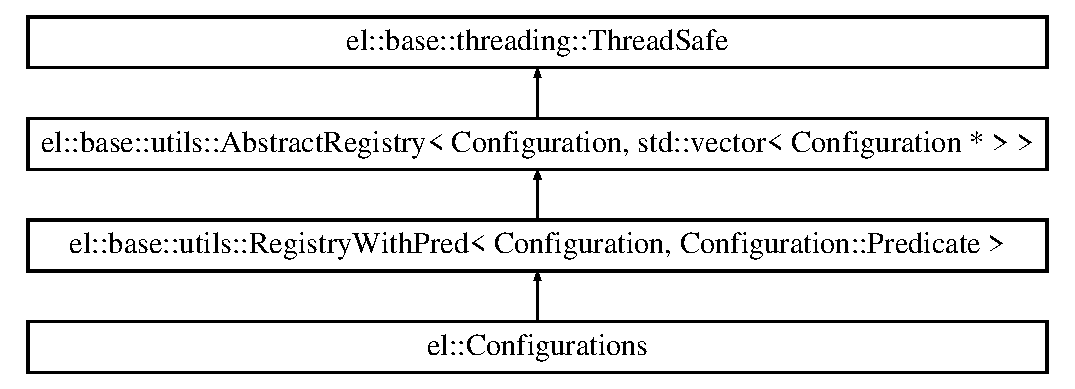
\includegraphics[height=4.000000cm]{classel_1_1_configurations}
\end{center}
\end{figure}
\subsection*{Classes}
\begin{DoxyCompactItemize}
\item 
class \hyperlink{classel_1_1_configurations_1_1_parser}{Parser}
\begin{DoxyCompactList}\small\item\em \hyperlink{classel_1_1_configurations_1_1_parser}{Parser} used internally to parse configurations from file or text. \end{DoxyCompactList}\end{DoxyCompactItemize}
\subsection*{Public Member Functions}
\begin{DoxyCompactItemize}
\item 
\hyperlink{classel_1_1_configurations_ae299dd1b60a1df9c013cc23029242a77}{Configurations} (void)
\begin{DoxyCompactList}\small\item\em Default constructor with empty repository. \end{DoxyCompactList}\item 
\hyperlink{classel_1_1_configurations_ae341bd647734d1180a5a138222d2f1ea}{Configurations} (const std\+::string \&\hyperlink{classel_1_1_configurations_a18df64bb5cd97bee672160290133141c}{configuration\+File}, bool use\+Defaults\+For\+Remaining=true, \hyperlink{classel_1_1_configurations}{Configurations} $\ast$base=nullptr)
\begin{DoxyCompactList}\small\item\em Constructor used to set configurations using configuration file. \end{DoxyCompactList}\item 
virtual \hyperlink{classel_1_1_configurations_aed56020af78d32cb4d3e4ac73abf3349}{$\sim$\+Configurations} (void)
\item 
bool \hyperlink{classel_1_1_configurations_aaa098126d64a5ee04a3944b1a65dcdca}{parse\+From\+File} (const std\+::string \&\hyperlink{classel_1_1_configurations_a18df64bb5cd97bee672160290133141c}{configuration\+File}, \hyperlink{classel_1_1_configurations}{Configurations} $\ast$base=nullptr)
\begin{DoxyCompactList}\small\item\em Parses configuration from file. \end{DoxyCompactList}\item 
bool \hyperlink{classel_1_1_configurations_af262a41dff665a11889261137b62af4a}{parse\+From\+Text} (const std\+::string \&configurations\+String, \hyperlink{classel_1_1_configurations}{Configurations} $\ast$base=nullptr)
\begin{DoxyCompactList}\small\item\em Parse configurations from configuration string. \end{DoxyCompactList}\item 
void \hyperlink{classel_1_1_configurations_a4c6db218908b39d23cc09b1a16a18e83}{set\+From\+Base} (\hyperlink{classel_1_1_configurations}{Configurations} $\ast$base)
\begin{DoxyCompactList}\small\item\em Sets configuration based-\/off an existing configurations. \end{DoxyCompactList}\item 
bool \hyperlink{classel_1_1_configurations_a1e812370f896b6429bf46b31fcd4e3e0}{has\+Configuration} (\hyperlink{namespaceel_a281f5db6d6163678bc68a8b23b59e124}{Configuration\+Type} configuration\+Type)
\begin{DoxyCompactList}\small\item\em Determines whether or not specified configuration type exists in the repository. \end{DoxyCompactList}\item 
bool \hyperlink{classel_1_1_configurations_a5313557efac3b0c78f973a5a1d685277}{has\+Configuration} (\hyperlink{namespaceel_ab0ac6091262344c52dd2d3ad099e8e36}{Level} level, \hyperlink{namespaceel_a281f5db6d6163678bc68a8b23b59e124}{Configuration\+Type} configuration\+Type)
\begin{DoxyCompactList}\small\item\em Determines whether or not specified configuration type exists for specified level. \end{DoxyCompactList}\item 
void \hyperlink{classel_1_1_configurations_a332717de96efc851a202b7afcc5e395c}{set} (\hyperlink{namespaceel_ab0ac6091262344c52dd2d3ad099e8e36}{Level} level, \hyperlink{namespaceel_a281f5db6d6163678bc68a8b23b59e124}{Configuration\+Type} configuration\+Type, const std\+::string \&value)
\begin{DoxyCompactList}\small\item\em Sets value of configuration for specified level. \end{DoxyCompactList}\item 
void \hyperlink{classel_1_1_configurations_a0ab07520b9409fe9f2c16a705d6936f1}{set} (\hyperlink{classel_1_1_configuration}{Configuration} $\ast$conf)
\begin{DoxyCompactList}\small\item\em Sets single configuration based on other single configuration. \end{DoxyCompactList}\item 
\hyperlink{classel_1_1_configuration}{Configuration} $\ast$ \hyperlink{classel_1_1_configurations_a6da4bc9bd6a14dc44feaf25163e998ca}{get} (\hyperlink{namespaceel_ab0ac6091262344c52dd2d3ad099e8e36}{Level} level, \hyperlink{namespaceel_a281f5db6d6163678bc68a8b23b59e124}{Configuration\+Type} configuration\+Type)
\item 
void \hyperlink{classel_1_1_configurations_a56c82c15ea39cc230a5c85ec2c41cbfd}{set\+Globally} (\hyperlink{namespaceel_a281f5db6d6163678bc68a8b23b59e124}{Configuration\+Type} configuration\+Type, const std\+::string \&value)
\begin{DoxyCompactList}\small\item\em Sets configuration for all levels. \end{DoxyCompactList}\item 
void \hyperlink{classel_1_1_configurations_a2a13be6154439286a68d2eccf8417edf}{clear} (void)
\begin{DoxyCompactList}\small\item\em Clears repository so that all the configurations are unset. \end{DoxyCompactList}\item 
const std\+::string \& \hyperlink{classel_1_1_configurations_a18df64bb5cd97bee672160290133141c}{configuration\+File} (void) const 
\begin{DoxyCompactList}\small\item\em Gets configuration file used in parsing this configurations. \end{DoxyCompactList}\item 
void \hyperlink{classel_1_1_configurations_ab34fa2ed4ac77f47b41e464c2d186239}{set\+To\+Default} (void)
\begin{DoxyCompactList}\small\item\em Sets configurations to \char`\"{}factory based\char`\"{} configurations. \end{DoxyCompactList}\item 
void \hyperlink{classel_1_1_configurations_ad89b7d2dd750e4d1b3deff800e278fdb}{set\+Remaining\+To\+Default} (void)
\begin{DoxyCompactList}\small\item\em Lets you set the remaining configurations to default. \end{DoxyCompactList}\end{DoxyCompactItemize}
\subsection*{Friends}
\begin{DoxyCompactItemize}
\item 
class \hyperlink{classel_1_1_configurations_a6efe246b312d02731fb0e1d120c0331d}{el\+::\+Loggers}
\end{DoxyCompactItemize}
\subsection*{Additional Inherited Members}


\subsection{Detailed Description}
Thread-\/safe \hyperlink{classel_1_1_configuration}{Configuration} repository. 

This repository represents configurations for all the levels and configuration type mapped to a value. 

Definition at line 2437 of file easylogging++.\+h.



\subsection{Constructor \& Destructor Documentation}
\hypertarget{classel_1_1_configurations_ae299dd1b60a1df9c013cc23029242a77}{}\index{el\+::\+Configurations@{el\+::\+Configurations}!Configurations@{Configurations}}
\index{Configurations@{Configurations}!el\+::\+Configurations@{el\+::\+Configurations}}
\subsubsection[{Configurations}]{\setlength{\rightskip}{0pt plus 5cm}el\+::\+Configurations\+::\+Configurations (
\begin{DoxyParamCaption}
\item[{void}]{}
\end{DoxyParamCaption}
)\hspace{0.3cm}{\ttfamily [inline]}}\label{classel_1_1_configurations_ae299dd1b60a1df9c013cc23029242a77}


Default constructor with empty repository. 



Definition at line 2440 of file easylogging++.\+h.

\hypertarget{classel_1_1_configurations_ae341bd647734d1180a5a138222d2f1ea}{}\index{el\+::\+Configurations@{el\+::\+Configurations}!Configurations@{Configurations}}
\index{Configurations@{Configurations}!el\+::\+Configurations@{el\+::\+Configurations}}
\subsubsection[{Configurations}]{\setlength{\rightskip}{0pt plus 5cm}el\+::\+Configurations\+::\+Configurations (
\begin{DoxyParamCaption}
\item[{const std\+::string \&}]{configuration\+File, }
\item[{bool}]{use\+Defaults\+For\+Remaining = {\ttfamily true}, }
\item[{{\bf Configurations} $\ast$}]{base = {\ttfamily nullptr}}
\end{DoxyParamCaption}
)\hspace{0.3cm}{\ttfamily [inline]}}\label{classel_1_1_configurations_ae341bd647734d1180a5a138222d2f1ea}


Constructor used to set configurations using configuration file. 


\begin{DoxyParams}{Parameters}
{\em configuration\+File} & Full path to configuration file \\
\hline
{\em use\+Defaults\+For\+Remaining} & Lets you set the remaining configurations to default. \\
\hline
{\em base} & If provided, this configuration will be based off existing repository that this argument is pointing to. \\
\hline
\end{DoxyParams}
\begin{DoxySeeAlso}{See also}
\hyperlink{classel_1_1_configurations_aaa098126d64a5ee04a3944b1a65dcdca}{parse\+From\+File(const std\+::string\&, Configurations$\ast$ base)} 

\hyperlink{classel_1_1_configurations_ad89b7d2dd750e4d1b3deff800e278fdb}{set\+Remaining\+To\+Default()} 
\end{DoxySeeAlso}


Definition at line 2451 of file easylogging++.\+h.

\hypertarget{classel_1_1_configurations_aed56020af78d32cb4d3e4ac73abf3349}{}\index{el\+::\+Configurations@{el\+::\+Configurations}!````~Configurations@{$\sim$\+Configurations}}
\index{````~Configurations@{$\sim$\+Configurations}!el\+::\+Configurations@{el\+::\+Configurations}}
\subsubsection[{$\sim$\+Configurations}]{\setlength{\rightskip}{0pt plus 5cm}virtual el\+::\+Configurations\+::$\sim$\+Configurations (
\begin{DoxyParamCaption}
\item[{void}]{}
\end{DoxyParamCaption}
)\hspace{0.3cm}{\ttfamily [inline]}, {\ttfamily [virtual]}}\label{classel_1_1_configurations_aed56020af78d32cb4d3e4ac73abf3349}


Definition at line 2460 of file easylogging++.\+h.



\subsection{Member Function Documentation}
\hypertarget{classel_1_1_configurations_a2a13be6154439286a68d2eccf8417edf}{}\index{el\+::\+Configurations@{el\+::\+Configurations}!clear@{clear}}
\index{clear@{clear}!el\+::\+Configurations@{el\+::\+Configurations}}
\subsubsection[{clear}]{\setlength{\rightskip}{0pt plus 5cm}void el\+::\+Configurations\+::clear (
\begin{DoxyParamCaption}
\item[{void}]{}
\end{DoxyParamCaption}
)\hspace{0.3cm}{\ttfamily [inline]}}\label{classel_1_1_configurations_a2a13be6154439286a68d2eccf8417edf}


Clears repository so that all the configurations are unset. 



Definition at line 2584 of file easylogging++.\+h.

\hypertarget{classel_1_1_configurations_a18df64bb5cd97bee672160290133141c}{}\index{el\+::\+Configurations@{el\+::\+Configurations}!configuration\+File@{configuration\+File}}
\index{configuration\+File@{configuration\+File}!el\+::\+Configurations@{el\+::\+Configurations}}
\subsubsection[{configuration\+File}]{\setlength{\rightskip}{0pt plus 5cm}const std\+::string\& el\+::\+Configurations\+::configuration\+File (
\begin{DoxyParamCaption}
\item[{void}]{}
\end{DoxyParamCaption}
) const\hspace{0.3cm}{\ttfamily [inline]}}\label{classel_1_1_configurations_a18df64bb5cd97bee672160290133141c}


Gets configuration file used in parsing this configurations. 

If this repository was set manually or by text this returns empty string. 

Definition at line 2592 of file easylogging++.\+h.

\hypertarget{classel_1_1_configurations_a6da4bc9bd6a14dc44feaf25163e998ca}{}\index{el\+::\+Configurations@{el\+::\+Configurations}!get@{get}}
\index{get@{get}!el\+::\+Configurations@{el\+::\+Configurations}}
\subsubsection[{get}]{\setlength{\rightskip}{0pt plus 5cm}{\bf Configuration}$\ast$ el\+::\+Configurations\+::get (
\begin{DoxyParamCaption}
\item[{{\bf Level}}]{level, }
\item[{{\bf Configuration\+Type}}]{configuration\+Type}
\end{DoxyParamCaption}
)\hspace{0.3cm}{\ttfamily [inline]}}\label{classel_1_1_configurations_a6da4bc9bd6a14dc44feaf25163e998ca}


Definition at line 2570 of file easylogging++.\+h.

\hypertarget{classel_1_1_configurations_a1e812370f896b6429bf46b31fcd4e3e0}{}\index{el\+::\+Configurations@{el\+::\+Configurations}!has\+Configuration@{has\+Configuration}}
\index{has\+Configuration@{has\+Configuration}!el\+::\+Configurations@{el\+::\+Configurations}}
\subsubsection[{has\+Configuration}]{\setlength{\rightskip}{0pt plus 5cm}bool el\+::\+Configurations\+::has\+Configuration (
\begin{DoxyParamCaption}
\item[{{\bf Configuration\+Type}}]{configuration\+Type}
\end{DoxyParamCaption}
)\hspace{0.3cm}{\ttfamily [inline]}}\label{classel_1_1_configurations_a1e812370f896b6429bf46b31fcd4e3e0}


Determines whether or not specified configuration type exists in the repository. 

Returns as soon as first level is found. 
\begin{DoxyParams}{Parameters}
{\em configuration\+Type} & Type of configuration to check existence for. \\
\hline
\end{DoxyParams}


Definition at line 2515 of file easylogging++.\+h.

\hypertarget{classel_1_1_configurations_a5313557efac3b0c78f973a5a1d685277}{}\index{el\+::\+Configurations@{el\+::\+Configurations}!has\+Configuration@{has\+Configuration}}
\index{has\+Configuration@{has\+Configuration}!el\+::\+Configurations@{el\+::\+Configurations}}
\subsubsection[{has\+Configuration}]{\setlength{\rightskip}{0pt plus 5cm}bool el\+::\+Configurations\+::has\+Configuration (
\begin{DoxyParamCaption}
\item[{{\bf Level}}]{level, }
\item[{{\bf Configuration\+Type}}]{configuration\+Type}
\end{DoxyParamCaption}
)\hspace{0.3cm}{\ttfamily [inline]}}\label{classel_1_1_configurations_a5313557efac3b0c78f973a5a1d685277}


Determines whether or not specified configuration type exists for specified level. 


\begin{DoxyParams}{Parameters}
{\em level} & Level to check \\
\hline
{\em configuration\+Type} & Type of configuration to check existence for. \\
\hline
\end{DoxyParams}


Definition at line 2530 of file easylogging++.\+h.

\hypertarget{classel_1_1_configurations_aaa098126d64a5ee04a3944b1a65dcdca}{}\index{el\+::\+Configurations@{el\+::\+Configurations}!parse\+From\+File@{parse\+From\+File}}
\index{parse\+From\+File@{parse\+From\+File}!el\+::\+Configurations@{el\+::\+Configurations}}
\subsubsection[{parse\+From\+File}]{\setlength{\rightskip}{0pt plus 5cm}bool el\+::\+Configurations\+::parse\+From\+File (
\begin{DoxyParamCaption}
\item[{const std\+::string \&}]{configuration\+File, }
\item[{{\bf Configurations} $\ast$}]{base = {\ttfamily nullptr}}
\end{DoxyParamCaption}
)\hspace{0.3cm}{\ttfamily [inline]}}\label{classel_1_1_configurations_aaa098126d64a5ee04a3944b1a65dcdca}


Parses configuration from file. 


\begin{DoxyParams}{Parameters}
{\em configuration\+File} & Full path to configuration file \\
\hline
{\em base} & \hyperlink{classel_1_1_configurations}{Configurations} to base new configuration repository off. This value is used when you want to use existing \hyperlink{classel_1_1_configurations}{Configurations} to base all the values and then set rest of configuration via configuration file. \\
\hline
\end{DoxyParams}
\begin{DoxyReturn}{Returns}
True if successfully parsed, false otherwise. You may define \textquotesingle{}E\+L\+P\+P\+\_\+\+D\+E\+B\+U\+G\+\_\+\+A\+S\+S\+E\+R\+T\+\_\+\+F\+A\+I\+L\+U\+R\+E\textquotesingle{} to make sure you do not proceed without successful parse. 
\end{DoxyReturn}


Definition at line 2469 of file easylogging++.\+h.

\hypertarget{classel_1_1_configurations_af262a41dff665a11889261137b62af4a}{}\index{el\+::\+Configurations@{el\+::\+Configurations}!parse\+From\+Text@{parse\+From\+Text}}
\index{parse\+From\+Text@{parse\+From\+Text}!el\+::\+Configurations@{el\+::\+Configurations}}
\subsubsection[{parse\+From\+Text}]{\setlength{\rightskip}{0pt plus 5cm}bool el\+::\+Configurations\+::parse\+From\+Text (
\begin{DoxyParamCaption}
\item[{const std\+::string \&}]{configurations\+String, }
\item[{{\bf Configurations} $\ast$}]{base = {\ttfamily nullptr}}
\end{DoxyParamCaption}
)\hspace{0.3cm}{\ttfamily [inline]}}\label{classel_1_1_configurations_af262a41dff665a11889261137b62af4a}


Parse configurations from configuration string. 

This configuration string has same syntax as configuration file contents. Make sure all the necessary new line characters are provided. 
\begin{DoxyParams}{Parameters}
{\em base} & \hyperlink{classel_1_1_configurations}{Configurations} to base new configuration repository off. This value is used when you want to use existing \hyperlink{classel_1_1_configurations}{Configurations} to base all the values and then set rest of configuration via configuration text. \\
\hline
\end{DoxyParams}
\begin{DoxyReturn}{Returns}
True if successfully parsed, false otherwise. You may define \textquotesingle{}E\+L\+P\+P\+\_\+\+D\+E\+B\+U\+G\+\_\+\+A\+S\+S\+E\+R\+T\+\_\+\+F\+A\+I\+L\+U\+R\+E\textquotesingle{} to make sure you do not proceed without successful parse. 
\end{DoxyReturn}


Definition at line 2491 of file easylogging++.\+h.

\hypertarget{classel_1_1_configurations_a332717de96efc851a202b7afcc5e395c}{}\index{el\+::\+Configurations@{el\+::\+Configurations}!set@{set}}
\index{set@{set}!el\+::\+Configurations@{el\+::\+Configurations}}
\subsubsection[{set}]{\setlength{\rightskip}{0pt plus 5cm}void el\+::\+Configurations\+::set (
\begin{DoxyParamCaption}
\item[{{\bf Level}}]{level, }
\item[{{\bf Configuration\+Type}}]{configuration\+Type, }
\item[{const std\+::string \&}]{value}
\end{DoxyParamCaption}
)\hspace{0.3cm}{\ttfamily [inline]}}\label{classel_1_1_configurations_a332717de96efc851a202b7afcc5e395c}


Sets value of configuration for specified level. 

Any existing configuration for specified level will be replaced. Also note that configuration types \hyperlink{namespaceel_a281f5db6d6163678bc68a8b23b59e124a052bf0f0c813b3c41c5b5046ebc26529}{Configuration\+Type\+::\+Milliseconds\+Width} and \hyperlink{namespaceel_a281f5db6d6163678bc68a8b23b59e124abe9e43d200c5698cb8519daed7035874}{Configuration\+Type\+::\+Performance\+Tracking} will be ignored if not set for \hyperlink{namespaceel_ab0ac6091262344c52dd2d3ad099e8e36a4cc6684df7b4a92b1dec6fce3264fac8}{Level\+::\+Global} because these configurations are not dependant on level. 
\begin{DoxyParams}{Parameters}
{\em level} & Level to set configuration for (\hyperlink{namespaceel_ab0ac6091262344c52dd2d3ad099e8e36}{el\+::\+Level}). \\
\hline
{\em configuration\+Type} & Type of configuration (\hyperlink{namespaceel_a281f5db6d6163678bc68a8b23b59e124}{el\+::\+Configuration\+Type}) \\
\hline
{\em value} & A string based value. Regardless of what the data type of configuration is, it will always be string from users\textquotesingle{} point of view. This is then parsed later to be used internally. \\
\hline
\end{DoxyParams}
\begin{DoxySeeAlso}{See also}
\hyperlink{classel_1_1_configuration_a04755de11422d7570869433ea157b705}{Configuration\+::set\+Value(const std\+::string\& value)} 

\hyperlink{namespaceel_ab0ac6091262344c52dd2d3ad099e8e36}{el\+::\+Level} 

\hyperlink{namespaceel_a281f5db6d6163678bc68a8b23b59e124}{el\+::\+Configuration\+Type} 
\end{DoxySeeAlso}


Definition at line 2553 of file easylogging++.\+h.

\hypertarget{classel_1_1_configurations_a0ab07520b9409fe9f2c16a705d6936f1}{}\index{el\+::\+Configurations@{el\+::\+Configurations}!set@{set}}
\index{set@{set}!el\+::\+Configurations@{el\+::\+Configurations}}
\subsubsection[{set}]{\setlength{\rightskip}{0pt plus 5cm}void el\+::\+Configurations\+::set (
\begin{DoxyParamCaption}
\item[{{\bf Configuration} $\ast$}]{conf}
\end{DoxyParamCaption}
)\hspace{0.3cm}{\ttfamily [inline]}}\label{classel_1_1_configurations_a0ab07520b9409fe9f2c16a705d6936f1}


Sets single configuration based on other single configuration. 

\begin{DoxySeeAlso}{See also}
\hyperlink{classel_1_1_configurations_a332717de96efc851a202b7afcc5e395c}{set(\+Level level, Configuration\+Type configuration\+Type, const std\+::string\& value)} 
\end{DoxySeeAlso}


Definition at line 2563 of file easylogging++.\+h.

\hypertarget{classel_1_1_configurations_a4c6db218908b39d23cc09b1a16a18e83}{}\index{el\+::\+Configurations@{el\+::\+Configurations}!set\+From\+Base@{set\+From\+Base}}
\index{set\+From\+Base@{set\+From\+Base}!el\+::\+Configurations@{el\+::\+Configurations}}
\subsubsection[{set\+From\+Base}]{\setlength{\rightskip}{0pt plus 5cm}void el\+::\+Configurations\+::set\+From\+Base (
\begin{DoxyParamCaption}
\item[{{\bf Configurations} $\ast$}]{base}
\end{DoxyParamCaption}
)\hspace{0.3cm}{\ttfamily [inline]}}\label{classel_1_1_configurations_a4c6db218908b39d23cc09b1a16a18e83}


Sets configuration based-\/off an existing configurations. 


\begin{DoxyParams}{Parameters}
{\em base} & Pointer to existing configurations. \\
\hline
\end{DoxyParams}


Definition at line 2501 of file easylogging++.\+h.

\hypertarget{classel_1_1_configurations_a56c82c15ea39cc230a5c85ec2c41cbfd}{}\index{el\+::\+Configurations@{el\+::\+Configurations}!set\+Globally@{set\+Globally}}
\index{set\+Globally@{set\+Globally}!el\+::\+Configurations@{el\+::\+Configurations}}
\subsubsection[{set\+Globally}]{\setlength{\rightskip}{0pt plus 5cm}void el\+::\+Configurations\+::set\+Globally (
\begin{DoxyParamCaption}
\item[{{\bf Configuration\+Type}}]{configuration\+Type, }
\item[{const std\+::string \&}]{value}
\end{DoxyParamCaption}
)\hspace{0.3cm}{\ttfamily [inline]}}\label{classel_1_1_configurations_a56c82c15ea39cc230a5c85ec2c41cbfd}


Sets configuration for all levels. 


\begin{DoxyParams}{Parameters}
{\em configuration\+Type} & Type of configuration \\
\hline
{\em value} & String based value \\
\hline
\end{DoxyParams}
\begin{DoxySeeAlso}{See also}
\hyperlink{classel_1_1_configurations_a332717de96efc851a202b7afcc5e395c}{Configurations\+::set(\+Level level, Configuration\+Type configuration\+Type, const std\+::string\& value)} 
\end{DoxySeeAlso}


Definition at line 2579 of file easylogging++.\+h.

\hypertarget{classel_1_1_configurations_ad89b7d2dd750e4d1b3deff800e278fdb}{}\index{el\+::\+Configurations@{el\+::\+Configurations}!set\+Remaining\+To\+Default@{set\+Remaining\+To\+Default}}
\index{set\+Remaining\+To\+Default@{set\+Remaining\+To\+Default}!el\+::\+Configurations@{el\+::\+Configurations}}
\subsubsection[{set\+Remaining\+To\+Default}]{\setlength{\rightskip}{0pt plus 5cm}void el\+::\+Configurations\+::set\+Remaining\+To\+Default (
\begin{DoxyParamCaption}
\item[{void}]{}
\end{DoxyParamCaption}
)\hspace{0.3cm}{\ttfamily [inline]}}\label{classel_1_1_configurations_ad89b7d2dd750e4d1b3deff800e278fdb}


Lets you set the remaining configurations to default. 

By remaining, it means that the level/type a configuration does not exist for. This function is useful when you want to minimize chances of failures, e.\+g, if you have a configuration file that sets configuration for all the configurations except for Enabled or not, we use this so that E\+N\+A\+B\+L\+E\+D is set to default i.\+e, true. If you dont do this explicitley (either by calling this function or by using second param in Constructor and try to access a value, an error is thrown 

Definition at line 2627 of file easylogging++.\+h.

\hypertarget{classel_1_1_configurations_ab34fa2ed4ac77f47b41e464c2d186239}{}\index{el\+::\+Configurations@{el\+::\+Configurations}!set\+To\+Default@{set\+To\+Default}}
\index{set\+To\+Default@{set\+To\+Default}!el\+::\+Configurations@{el\+::\+Configurations}}
\subsubsection[{set\+To\+Default}]{\setlength{\rightskip}{0pt plus 5cm}void el\+::\+Configurations\+::set\+To\+Default (
\begin{DoxyParamCaption}
\item[{void}]{}
\end{DoxyParamCaption}
)\hspace{0.3cm}{\ttfamily [inline]}}\label{classel_1_1_configurations_ab34fa2ed4ac77f47b41e464c2d186239}


Sets configurations to \char`\"{}factory based\char`\"{} configurations. 



Definition at line 2597 of file easylogging++.\+h.



\subsection{Friends And Related Function Documentation}
\hypertarget{classel_1_1_configurations_a6efe246b312d02731fb0e1d120c0331d}{}\index{el\+::\+Configurations@{el\+::\+Configurations}!el\+::\+Loggers@{el\+::\+Loggers}}
\index{el\+::\+Loggers@{el\+::\+Loggers}!el\+::\+Configurations@{el\+::\+Configurations}}
\subsubsection[{el\+::\+Loggers}]{\setlength{\rightskip}{0pt plus 5cm}friend class {\bf el\+::\+Loggers}\hspace{0.3cm}{\ttfamily [friend]}}\label{classel_1_1_configurations_a6efe246b312d02731fb0e1d120c0331d}


Definition at line 2801 of file easylogging++.\+h.



The documentation for this class was generated from the following file\+:\begin{DoxyCompactItemize}
\item 
lib/\hyperlink{easylogging_09_09_8h}{easylogging++.\+h}\end{DoxyCompactItemize}

\hypertarget{classel_1_1_configuration_type_helper}{}\section{el\+:\+:Configuration\+Type\+Helper Class Reference}
\label{classel_1_1_configuration_type_helper}\index{el\+::\+Configuration\+Type\+Helper@{el\+::\+Configuration\+Type\+Helper}}


Static class that contains helper functions for \hyperlink{namespaceel_a281f5db6d6163678bc68a8b23b59e124}{el\+::\+Configuration\+Type}.  




{\ttfamily \#include $<$easylogging++.\+h$>$}

Inheritance diagram for el\+:\+:Configuration\+Type\+Helper\+:\begin{figure}[H]
\begin{center}
\leavevmode
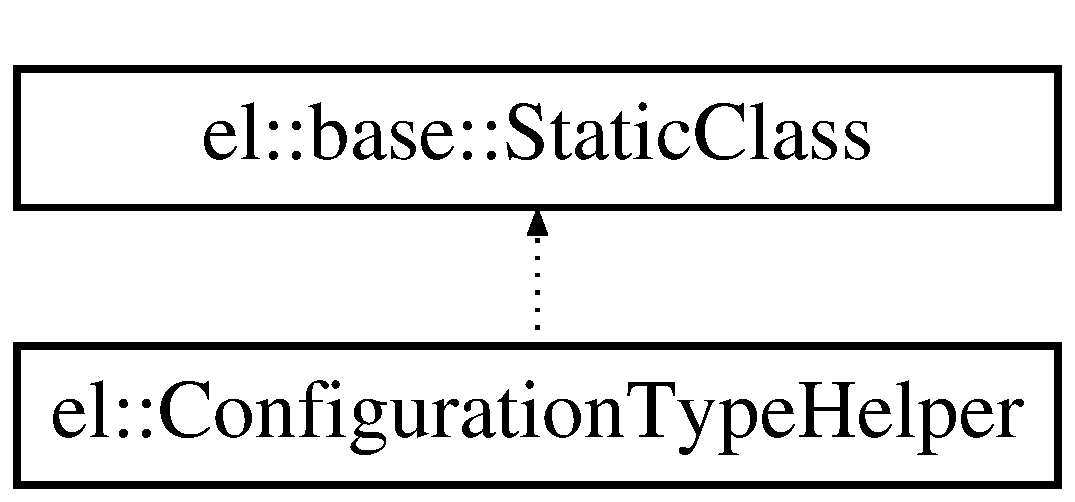
\includegraphics[height=2.000000cm]{classel_1_1_configuration_type_helper}
\end{center}
\end{figure}
\subsection*{Static Public Member Functions}
\begin{DoxyCompactItemize}
\item 
static \hyperlink{namespaceel_1_1base_1_1type_afb892a99b7545bf6e45c1e1d84af2ec9}{base\+::type\+::\+Enum\+Type} \hyperlink{classel_1_1_configuration_type_helper_aa53161071fee3ce3f371ab90c62d5fc2}{cast\+To\+Int} (\hyperlink{namespaceel_a281f5db6d6163678bc68a8b23b59e124}{Configuration\+Type} configuration\+Type)
\begin{DoxyCompactList}\small\item\em Casts configuration type to int, useful for iterating through enum. \end{DoxyCompactList}\item 
static \hyperlink{namespaceel_a281f5db6d6163678bc68a8b23b59e124}{Configuration\+Type} \hyperlink{classel_1_1_configuration_type_helper_a62301cbc966cf7e7e2a7b55cc3259996}{cast\+From\+Int} (\hyperlink{namespaceel_1_1base_1_1type_afb892a99b7545bf6e45c1e1d84af2ec9}{base\+::type\+::\+Enum\+Type} c)
\begin{DoxyCompactList}\small\item\em Casts int(ushort) to configurationt type, useful for iterating through enum. \end{DoxyCompactList}\item 
static const char $\ast$ \hyperlink{classel_1_1_configuration_type_helper_ad7f0a19c416c4a8ddaf85330b141383c}{convert\+To\+String} (\hyperlink{namespaceel_a281f5db6d6163678bc68a8b23b59e124}{Configuration\+Type} configuration\+Type)
\begin{DoxyCompactList}\small\item\em Converts configuration type to associated const char$\ast$. \end{DoxyCompactList}\item 
static \hyperlink{namespaceel_a281f5db6d6163678bc68a8b23b59e124}{Configuration\+Type} \hyperlink{classel_1_1_configuration_type_helper_af4a35305e3941fd578e55fec624eba43}{convert\+From\+String} (const char $\ast$config\+Str)
\begin{DoxyCompactList}\small\item\em Converts from config\+Str to Configuration\+Type. \end{DoxyCompactList}\item 
static void \hyperlink{classel_1_1_configuration_type_helper_aa0524147f792309fc09e0b8d14826c17}{for\+Each\+Config\+Type} (\hyperlink{namespaceel_1_1base_1_1type_afb892a99b7545bf6e45c1e1d84af2ec9}{base\+::type\+::\+Enum\+Type} $\ast$start\+Index, const std\+::function$<$ bool(void)$>$ \&fn)
\begin{DoxyCompactList}\small\item\em Applies specified function to each configuration type starting from start\+Index. \end{DoxyCompactList}\end{DoxyCompactItemize}
\subsection*{Static Public Attributes}
\begin{DoxyCompactItemize}
\item 
static const \hyperlink{namespaceel_1_1base_1_1type_afb892a99b7545bf6e45c1e1d84af2ec9}{base\+::type\+::\+Enum\+Type} \hyperlink{classel_1_1_configuration_type_helper_ab7266e698eb32dec2da285325a66e322}{k\+Min\+Valid} = static\+\_\+cast$<$\hyperlink{namespaceel_1_1base_1_1type_afb892a99b7545bf6e45c1e1d84af2ec9}{base\+::type\+::\+Enum\+Type}$>$(\hyperlink{namespaceel_a281f5db6d6163678bc68a8b23b59e124a00d23a76e43b46dae9ec7aa9dcbebb32}{Configuration\+Type\+::\+Enabled})
\begin{DoxyCompactList}\small\item\em Represents minimum valid configuration type. Useful when iterating through enum. \end{DoxyCompactList}\item 
static const \hyperlink{namespaceel_1_1base_1_1type_afb892a99b7545bf6e45c1e1d84af2ec9}{base\+::type\+::\+Enum\+Type} \hyperlink{classel_1_1_configuration_type_helper_aa02f3cefb127e7eb97d7e1dd7f51a12d}{k\+Max\+Valid} = static\+\_\+cast$<$\hyperlink{namespaceel_1_1base_1_1type_afb892a99b7545bf6e45c1e1d84af2ec9}{base\+::type\+::\+Enum\+Type}$>$(\hyperlink{namespaceel_a281f5db6d6163678bc68a8b23b59e124a4b35e615142d60db6383426f051e700b}{Configuration\+Type\+::\+Max\+Log\+File\+Size})
\begin{DoxyCompactList}\small\item\em Represents maximum valid configuration type. This is used internally and you should not need it. \end{DoxyCompactList}\end{DoxyCompactItemize}


\subsection{Detailed Description}
Static class that contains helper functions for \hyperlink{namespaceel_a281f5db6d6163678bc68a8b23b59e124}{el\+::\+Configuration\+Type}. 

Definition at line 619 of file easylogging++.\+h.



\subsection{Member Function Documentation}
\hypertarget{classel_1_1_configuration_type_helper_a62301cbc966cf7e7e2a7b55cc3259996}{}\index{el\+::\+Configuration\+Type\+Helper@{el\+::\+Configuration\+Type\+Helper}!cast\+From\+Int@{cast\+From\+Int}}
\index{cast\+From\+Int@{cast\+From\+Int}!el\+::\+Configuration\+Type\+Helper@{el\+::\+Configuration\+Type\+Helper}}
\subsubsection[{cast\+From\+Int}]{\setlength{\rightskip}{0pt plus 5cm}static {\bf Configuration\+Type} el\+::\+Configuration\+Type\+Helper\+::cast\+From\+Int (
\begin{DoxyParamCaption}
\item[{{\bf base\+::type\+::\+Enum\+Type}}]{c}
\end{DoxyParamCaption}
)\hspace{0.3cm}{\ttfamily [inline]}, {\ttfamily [static]}}\label{classel_1_1_configuration_type_helper_a62301cbc966cf7e7e2a7b55cc3259996}


Casts int(ushort) to configurationt type, useful for iterating through enum. 



Definition at line 630 of file easylogging++.\+h.

\hypertarget{classel_1_1_configuration_type_helper_aa53161071fee3ce3f371ab90c62d5fc2}{}\index{el\+::\+Configuration\+Type\+Helper@{el\+::\+Configuration\+Type\+Helper}!cast\+To\+Int@{cast\+To\+Int}}
\index{cast\+To\+Int@{cast\+To\+Int}!el\+::\+Configuration\+Type\+Helper@{el\+::\+Configuration\+Type\+Helper}}
\subsubsection[{cast\+To\+Int}]{\setlength{\rightskip}{0pt plus 5cm}static {\bf base\+::type\+::\+Enum\+Type} el\+::\+Configuration\+Type\+Helper\+::cast\+To\+Int (
\begin{DoxyParamCaption}
\item[{{\bf Configuration\+Type}}]{configuration\+Type}
\end{DoxyParamCaption}
)\hspace{0.3cm}{\ttfamily [inline]}, {\ttfamily [static]}}\label{classel_1_1_configuration_type_helper_aa53161071fee3ce3f371ab90c62d5fc2}


Casts configuration type to int, useful for iterating through enum. 



Definition at line 626 of file easylogging++.\+h.

\hypertarget{classel_1_1_configuration_type_helper_af4a35305e3941fd578e55fec624eba43}{}\index{el\+::\+Configuration\+Type\+Helper@{el\+::\+Configuration\+Type\+Helper}!convert\+From\+String@{convert\+From\+String}}
\index{convert\+From\+String@{convert\+From\+String}!el\+::\+Configuration\+Type\+Helper@{el\+::\+Configuration\+Type\+Helper}}
\subsubsection[{convert\+From\+String}]{\setlength{\rightskip}{0pt plus 5cm}static {\bf Configuration\+Type} el\+::\+Configuration\+Type\+Helper\+::convert\+From\+String (
\begin{DoxyParamCaption}
\item[{const char $\ast$}]{config\+Str}
\end{DoxyParamCaption}
)\hspace{0.3cm}{\ttfamily [inline]}, {\ttfamily [static]}}\label{classel_1_1_configuration_type_helper_af4a35305e3941fd578e55fec624eba43}


Converts from config\+Str to Configuration\+Type. 


\begin{DoxyParams}{Parameters}
{\em config\+Str} & Upper case string based configuration type. Lower case is also valid but providing upper case is recommended. \\
\hline
\end{DoxyParams}


Definition at line 651 of file easylogging++.\+h.

\hypertarget{classel_1_1_configuration_type_helper_ad7f0a19c416c4a8ddaf85330b141383c}{}\index{el\+::\+Configuration\+Type\+Helper@{el\+::\+Configuration\+Type\+Helper}!convert\+To\+String@{convert\+To\+String}}
\index{convert\+To\+String@{convert\+To\+String}!el\+::\+Configuration\+Type\+Helper@{el\+::\+Configuration\+Type\+Helper}}
\subsubsection[{convert\+To\+String}]{\setlength{\rightskip}{0pt plus 5cm}static const char$\ast$ el\+::\+Configuration\+Type\+Helper\+::convert\+To\+String (
\begin{DoxyParamCaption}
\item[{{\bf Configuration\+Type}}]{configuration\+Type}
\end{DoxyParamCaption}
)\hspace{0.3cm}{\ttfamily [inline]}, {\ttfamily [static]}}\label{classel_1_1_configuration_type_helper_ad7f0a19c416c4a8ddaf85330b141383c}


Converts configuration type to associated const char$\ast$. 

\begin{DoxyReturn}{Returns}
Upper case string based configuration type. 
\end{DoxyReturn}


Definition at line 635 of file easylogging++.\+h.

\hypertarget{classel_1_1_configuration_type_helper_aa0524147f792309fc09e0b8d14826c17}{}\index{el\+::\+Configuration\+Type\+Helper@{el\+::\+Configuration\+Type\+Helper}!for\+Each\+Config\+Type@{for\+Each\+Config\+Type}}
\index{for\+Each\+Config\+Type@{for\+Each\+Config\+Type}!el\+::\+Configuration\+Type\+Helper@{el\+::\+Configuration\+Type\+Helper}}
\subsubsection[{for\+Each\+Config\+Type}]{\setlength{\rightskip}{0pt plus 5cm}static void el\+::\+Configuration\+Type\+Helper\+::for\+Each\+Config\+Type (
\begin{DoxyParamCaption}
\item[{{\bf base\+::type\+::\+Enum\+Type} $\ast$}]{start\+Index, }
\item[{const std\+::function$<$ bool(void)$>$ \&}]{fn}
\end{DoxyParamCaption}
)\hspace{0.3cm}{\ttfamily [inline]}, {\ttfamily [static]}}\label{classel_1_1_configuration_type_helper_aa0524147f792309fc09e0b8d14826c17}


Applies specified function to each configuration type starting from start\+Index. 


\begin{DoxyParams}{Parameters}
{\em start\+Index} & initial value to start the iteration from. This is passed by pointer and is left-\/shifted so this can be used inside function (fn) to represent current configuration type. \\
\hline
{\em fn} & function to apply with each configuration type. This bool represent whether or not to stop iterating through configurations. \\
\hline
\end{DoxyParams}


Definition at line 677 of file easylogging++.\+h.



\subsection{Member Data Documentation}
\hypertarget{classel_1_1_configuration_type_helper_aa02f3cefb127e7eb97d7e1dd7f51a12d}{}\index{el\+::\+Configuration\+Type\+Helper@{el\+::\+Configuration\+Type\+Helper}!k\+Max\+Valid@{k\+Max\+Valid}}
\index{k\+Max\+Valid@{k\+Max\+Valid}!el\+::\+Configuration\+Type\+Helper@{el\+::\+Configuration\+Type\+Helper}}
\subsubsection[{k\+Max\+Valid}]{\setlength{\rightskip}{0pt plus 5cm}const {\bf base\+::type\+::\+Enum\+Type} el\+::\+Configuration\+Type\+Helper\+::k\+Max\+Valid = static\+\_\+cast$<${\bf base\+::type\+::\+Enum\+Type}$>$({\bf Configuration\+Type\+::\+Max\+Log\+File\+Size})\hspace{0.3cm}{\ttfamily [static]}}\label{classel_1_1_configuration_type_helper_aa02f3cefb127e7eb97d7e1dd7f51a12d}


Represents maximum valid configuration type. This is used internally and you should not need it. 



Definition at line 624 of file easylogging++.\+h.

\hypertarget{classel_1_1_configuration_type_helper_ab7266e698eb32dec2da285325a66e322}{}\index{el\+::\+Configuration\+Type\+Helper@{el\+::\+Configuration\+Type\+Helper}!k\+Min\+Valid@{k\+Min\+Valid}}
\index{k\+Min\+Valid@{k\+Min\+Valid}!el\+::\+Configuration\+Type\+Helper@{el\+::\+Configuration\+Type\+Helper}}
\subsubsection[{k\+Min\+Valid}]{\setlength{\rightskip}{0pt plus 5cm}const {\bf base\+::type\+::\+Enum\+Type} el\+::\+Configuration\+Type\+Helper\+::k\+Min\+Valid = static\+\_\+cast$<${\bf base\+::type\+::\+Enum\+Type}$>$({\bf Configuration\+Type\+::\+Enabled})\hspace{0.3cm}{\ttfamily [static]}}\label{classel_1_1_configuration_type_helper_ab7266e698eb32dec2da285325a66e322}


Represents minimum valid configuration type. Useful when iterating through enum. 



Definition at line 622 of file easylogging++.\+h.



The documentation for this class was generated from the following file\+:\begin{DoxyCompactItemize}
\item 
lib/\hyperlink{easylogging_09_09_8h}{easylogging++.\+h}\end{DoxyCompactItemize}

\hypertarget{classel_1_1base_1_1debug_1_1_crash_handler}{}\section{el\+:\+:base\+:\+:debug\+:\+:Crash\+Handler Class Reference}
\label{classel_1_1base_1_1debug_1_1_crash_handler}\index{el\+::base\+::debug\+::\+Crash\+Handler@{el\+::base\+::debug\+::\+Crash\+Handler}}


Handles unexpected crashes.  




{\ttfamily \#include $<$easylogging++.\+h$>$}

Inheritance diagram for el\+:\+:base\+:\+:debug\+:\+:Crash\+Handler\+:\begin{figure}[H]
\begin{center}
\leavevmode
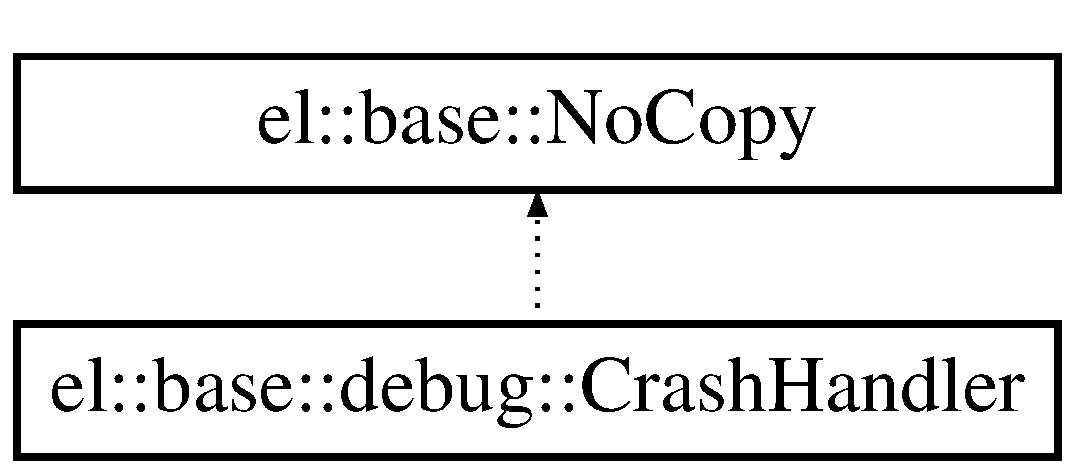
\includegraphics[height=2.000000cm]{classel_1_1base_1_1debug_1_1_crash_handler}
\end{center}
\end{figure}
\subsection*{Public Types}
\begin{DoxyCompactItemize}
\item 
typedef void($\ast$ \hyperlink{classel_1_1base_1_1debug_1_1_crash_handler_aebf80d2fd5180d9c56db5a7e9abc7ad9}{Handler}) (int)
\end{DoxyCompactItemize}
\subsection*{Public Member Functions}
\begin{DoxyCompactItemize}
\item 
\hyperlink{classel_1_1base_1_1debug_1_1_crash_handler_a1d1e1a77bb6c37b1fbb39ecf94b38983}{Crash\+Handler} (bool use\+Default)
\item 
\hyperlink{classel_1_1base_1_1debug_1_1_crash_handler_a9fbf8df7a292fcbeabfb87b241c83f78}{Crash\+Handler} (const \hyperlink{classel_1_1base_1_1debug_1_1_crash_handler_aebf80d2fd5180d9c56db5a7e9abc7ad9}{Handler} \&c\+Handler)
\item 
void \hyperlink{classel_1_1base_1_1debug_1_1_crash_handler_abd1d3d1ad5f1de2d40c39dd0542c26d4}{set\+Handler} (const \hyperlink{classel_1_1base_1_1debug_1_1_crash_handler_aebf80d2fd5180d9c56db5a7e9abc7ad9}{Handler} \&c\+Handler)
\end{DoxyCompactItemize}


\subsection{Detailed Description}
Handles unexpected crashes. 

Definition at line 5596 of file easylogging++.\+h.



\subsection{Member Typedef Documentation}
\hypertarget{classel_1_1base_1_1debug_1_1_crash_handler_aebf80d2fd5180d9c56db5a7e9abc7ad9}{}\index{el\+::base\+::debug\+::\+Crash\+Handler@{el\+::base\+::debug\+::\+Crash\+Handler}!Handler@{Handler}}
\index{Handler@{Handler}!el\+::base\+::debug\+::\+Crash\+Handler@{el\+::base\+::debug\+::\+Crash\+Handler}}
\subsubsection[{Handler}]{\setlength{\rightskip}{0pt plus 5cm}typedef void($\ast$ el\+::base\+::debug\+::\+Crash\+Handler\+::\+Handler) (int)}\label{classel_1_1base_1_1debug_1_1_crash_handler_aebf80d2fd5180d9c56db5a7e9abc7ad9}


Definition at line 5598 of file easylogging++.\+h.



\subsection{Constructor \& Destructor Documentation}
\hypertarget{classel_1_1base_1_1debug_1_1_crash_handler_a1d1e1a77bb6c37b1fbb39ecf94b38983}{}\index{el\+::base\+::debug\+::\+Crash\+Handler@{el\+::base\+::debug\+::\+Crash\+Handler}!Crash\+Handler@{Crash\+Handler}}
\index{Crash\+Handler@{Crash\+Handler}!el\+::base\+::debug\+::\+Crash\+Handler@{el\+::base\+::debug\+::\+Crash\+Handler}}
\subsubsection[{Crash\+Handler}]{\setlength{\rightskip}{0pt plus 5cm}el\+::base\+::debug\+::\+Crash\+Handler\+::\+Crash\+Handler (
\begin{DoxyParamCaption}
\item[{bool}]{use\+Default}
\end{DoxyParamCaption}
)\hspace{0.3cm}{\ttfamily [inline]}, {\ttfamily [explicit]}}\label{classel_1_1base_1_1debug_1_1_crash_handler_a1d1e1a77bb6c37b1fbb39ecf94b38983}


Definition at line 5600 of file easylogging++.\+h.

\hypertarget{classel_1_1base_1_1debug_1_1_crash_handler_a9fbf8df7a292fcbeabfb87b241c83f78}{}\index{el\+::base\+::debug\+::\+Crash\+Handler@{el\+::base\+::debug\+::\+Crash\+Handler}!Crash\+Handler@{Crash\+Handler}}
\index{Crash\+Handler@{Crash\+Handler}!el\+::base\+::debug\+::\+Crash\+Handler@{el\+::base\+::debug\+::\+Crash\+Handler}}
\subsubsection[{Crash\+Handler}]{\setlength{\rightskip}{0pt plus 5cm}el\+::base\+::debug\+::\+Crash\+Handler\+::\+Crash\+Handler (
\begin{DoxyParamCaption}
\item[{const {\bf Handler} \&}]{c\+Handler}
\end{DoxyParamCaption}
)\hspace{0.3cm}{\ttfamily [inline]}, {\ttfamily [explicit]}}\label{classel_1_1base_1_1debug_1_1_crash_handler_a9fbf8df7a292fcbeabfb87b241c83f78}


Definition at line 5605 of file easylogging++.\+h.



\subsection{Member Function Documentation}
\hypertarget{classel_1_1base_1_1debug_1_1_crash_handler_abd1d3d1ad5f1de2d40c39dd0542c26d4}{}\index{el\+::base\+::debug\+::\+Crash\+Handler@{el\+::base\+::debug\+::\+Crash\+Handler}!set\+Handler@{set\+Handler}}
\index{set\+Handler@{set\+Handler}!el\+::base\+::debug\+::\+Crash\+Handler@{el\+::base\+::debug\+::\+Crash\+Handler}}
\subsubsection[{set\+Handler}]{\setlength{\rightskip}{0pt plus 5cm}void el\+::base\+::debug\+::\+Crash\+Handler\+::set\+Handler (
\begin{DoxyParamCaption}
\item[{const {\bf Handler} \&}]{c\+Handler}
\end{DoxyParamCaption}
)\hspace{0.3cm}{\ttfamily [inline]}}\label{classel_1_1base_1_1debug_1_1_crash_handler_abd1d3d1ad5f1de2d40c39dd0542c26d4}


Definition at line 5608 of file easylogging++.\+h.



The documentation for this class was generated from the following file\+:\begin{DoxyCompactItemize}
\item 
lib/\hyperlink{easylogging_09_09_8h}{easylogging++.\+h}\end{DoxyCompactItemize}

\hypertarget{classel_1_1_custom_format_specifier}{}\section{el\+:\+:Custom\+Format\+Specifier Class Reference}
\label{classel_1_1_custom_format_specifier}\index{el\+::\+Custom\+Format\+Specifier@{el\+::\+Custom\+Format\+Specifier}}


User-\/provided custom format specifier.  




{\ttfamily \#include $<$easylogging++.\+h$>$}

\subsection*{Public Member Functions}
\begin{DoxyCompactItemize}
\item 
\hyperlink{classel_1_1_custom_format_specifier_a1d1bfa8b489d2908ee543023a51e58f6}{Custom\+Format\+Specifier} (const char $\ast$\hyperlink{classel_1_1_custom_format_specifier_a0be00787b7ca1caedd32e1627d76fd24}{format\+Specifier}, const \hyperlink{namespaceel_ab3cd18425a11df166a041d9024b8b5c6}{Format\+Specifier\+Value\+Resolver} \&\hyperlink{classel_1_1_custom_format_specifier_ac426e6771ae35e060313b8683b88adc8}{resolver})
\item 
const char $\ast$ \hyperlink{classel_1_1_custom_format_specifier_a0be00787b7ca1caedd32e1627d76fd24}{format\+Specifier} (void) const 
\item 
const \hyperlink{namespaceel_ab3cd18425a11df166a041d9024b8b5c6}{Format\+Specifier\+Value\+Resolver} \& \hyperlink{classel_1_1_custom_format_specifier_ac426e6771ae35e060313b8683b88adc8}{resolver} (void) const 
\item 
bool \hyperlink{classel_1_1_custom_format_specifier_ae17a9fbf8c5a28867308fcb8966a3aa0}{operator==} (const char $\ast$\hyperlink{classel_1_1_custom_format_specifier_a0be00787b7ca1caedd32e1627d76fd24}{format\+Specifier})
\end{DoxyCompactItemize}


\subsection{Detailed Description}
User-\/provided custom format specifier. 

\begin{DoxySeeAlso}{See also}
\hyperlink{classel_1_1_helpers_aa6de15a09db4f2a6763a6652c0ea12b1}{el\+::\+Helpers\+::install\+Custom\+Format\+Specifier} 

\hyperlink{namespaceel_ab3cd18425a11df166a041d9024b8b5c6}{Format\+Specifier\+Value\+Resolver} 
\end{DoxySeeAlso}


Definition at line 2335 of file easylogging++.\+h.



\subsection{Constructor \& Destructor Documentation}
\hypertarget{classel_1_1_custom_format_specifier_a1d1bfa8b489d2908ee543023a51e58f6}{}\index{el\+::\+Custom\+Format\+Specifier@{el\+::\+Custom\+Format\+Specifier}!Custom\+Format\+Specifier@{Custom\+Format\+Specifier}}
\index{Custom\+Format\+Specifier@{Custom\+Format\+Specifier}!el\+::\+Custom\+Format\+Specifier@{el\+::\+Custom\+Format\+Specifier}}
\subsubsection[{Custom\+Format\+Specifier}]{\setlength{\rightskip}{0pt plus 5cm}el\+::\+Custom\+Format\+Specifier\+::\+Custom\+Format\+Specifier (
\begin{DoxyParamCaption}
\item[{const char $\ast$}]{format\+Specifier, }
\item[{const {\bf Format\+Specifier\+Value\+Resolver} \&}]{resolver}
\end{DoxyParamCaption}
)\hspace{0.3cm}{\ttfamily [inline]}}\label{classel_1_1_custom_format_specifier_a1d1bfa8b489d2908ee543023a51e58f6}


Definition at line 2337 of file easylogging++.\+h.



\subsection{Member Function Documentation}
\hypertarget{classel_1_1_custom_format_specifier_a0be00787b7ca1caedd32e1627d76fd24}{}\index{el\+::\+Custom\+Format\+Specifier@{el\+::\+Custom\+Format\+Specifier}!format\+Specifier@{format\+Specifier}}
\index{format\+Specifier@{format\+Specifier}!el\+::\+Custom\+Format\+Specifier@{el\+::\+Custom\+Format\+Specifier}}
\subsubsection[{format\+Specifier}]{\setlength{\rightskip}{0pt plus 5cm}const char$\ast$ el\+::\+Custom\+Format\+Specifier\+::format\+Specifier (
\begin{DoxyParamCaption}
\item[{void}]{}
\end{DoxyParamCaption}
) const\hspace{0.3cm}{\ttfamily [inline]}}\label{classel_1_1_custom_format_specifier_a0be00787b7ca1caedd32e1627d76fd24}


Definition at line 2339 of file easylogging++.\+h.

\hypertarget{classel_1_1_custom_format_specifier_ae17a9fbf8c5a28867308fcb8966a3aa0}{}\index{el\+::\+Custom\+Format\+Specifier@{el\+::\+Custom\+Format\+Specifier}!operator==@{operator==}}
\index{operator==@{operator==}!el\+::\+Custom\+Format\+Specifier@{el\+::\+Custom\+Format\+Specifier}}
\subsubsection[{operator==}]{\setlength{\rightskip}{0pt plus 5cm}bool el\+::\+Custom\+Format\+Specifier\+::operator== (
\begin{DoxyParamCaption}
\item[{const char $\ast$}]{format\+Specifier}
\end{DoxyParamCaption}
)\hspace{0.3cm}{\ttfamily [inline]}}\label{classel_1_1_custom_format_specifier_ae17a9fbf8c5a28867308fcb8966a3aa0}


Definition at line 2341 of file easylogging++.\+h.

\hypertarget{classel_1_1_custom_format_specifier_ac426e6771ae35e060313b8683b88adc8}{}\index{el\+::\+Custom\+Format\+Specifier@{el\+::\+Custom\+Format\+Specifier}!resolver@{resolver}}
\index{resolver@{resolver}!el\+::\+Custom\+Format\+Specifier@{el\+::\+Custom\+Format\+Specifier}}
\subsubsection[{resolver}]{\setlength{\rightskip}{0pt plus 5cm}const {\bf Format\+Specifier\+Value\+Resolver}\& el\+::\+Custom\+Format\+Specifier\+::resolver (
\begin{DoxyParamCaption}
\item[{void}]{}
\end{DoxyParamCaption}
) const\hspace{0.3cm}{\ttfamily [inline]}}\label{classel_1_1_custom_format_specifier_ac426e6771ae35e060313b8683b88adc8}


Definition at line 2340 of file easylogging++.\+h.



The documentation for this class was generated from the following file\+:\begin{DoxyCompactItemize}
\item 
lib/\hyperlink{easylogging_09_09_8h}{easylogging++.\+h}\end{DoxyCompactItemize}

\hypertarget{class_database}{}\section{Database Class Reference}
\label{class_database}\index{Database@{Database}}


{\ttfamily \#include $<$Database.\+h$>$}

Inheritance diagram for Database\+:\begin{figure}[H]
\begin{center}
\leavevmode
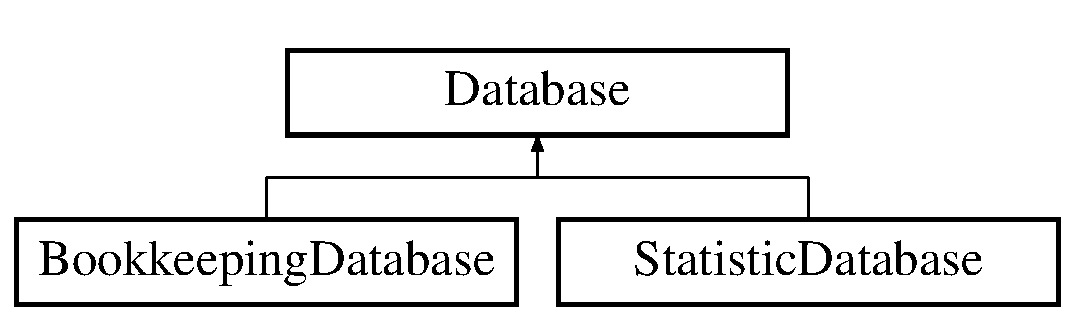
\includegraphics[height=2.000000cm]{class_database}
\end{center}
\end{figure}
\subsection*{Public Member Functions}
\begin{DoxyCompactItemize}
\item 
virtual void \hyperlink{class_database_aa80c3dd72d5b120a148ef31ccc7430b6}{insert\+Task\+Data} (string data)=0
\end{DoxyCompactItemize}


\subsection{Detailed Description}


Definition at line 17 of file Database.\+h.



\subsection{Member Function Documentation}
\hypertarget{class_database_aa80c3dd72d5b120a148ef31ccc7430b6}{}\index{Database@{Database}!insert\+Task\+Data@{insert\+Task\+Data}}
\index{insert\+Task\+Data@{insert\+Task\+Data}!Database@{Database}}
\subsubsection[{insert\+Task\+Data}]{\setlength{\rightskip}{0pt plus 5cm}virtual void Database\+::insert\+Task\+Data (
\begin{DoxyParamCaption}
\item[{string}]{data}
\end{DoxyParamCaption}
)\hspace{0.3cm}{\ttfamily [pure virtual]}}\label{class_database_aa80c3dd72d5b120a148ef31ccc7430b6}


Implemented in \hyperlink{class_bookkeeping_database_a16c4a4334e3c093df2e158f82bbbd09c}{Bookkeeping\+Database}, and \hyperlink{class_statistic_database_ab900a61b8b7bb8831310595ec218d9a7}{Statistic\+Database}.



The documentation for this class was generated from the following file\+:\begin{DoxyCompactItemize}
\item 
src/database/\hyperlink{_database_8h}{Database.\+h}\end{DoxyCompactItemize}

\hypertarget{class_database_handler}{}\section{Database\+Handler Class Reference}
\label{class_database_handler}\index{Database\+Handler@{Database\+Handler}}


{\ttfamily \#include $<$Database\+Handler.\+h$>$}

\subsection*{Public Member Functions}
\begin{DoxyCompactItemize}
\item 
\hyperlink{class_database_handler_ac27357d3431faf4fd6810483a24a43fd}{Database\+Handler} ()
\item 
string \hyperlink{class_database_handler_acb8ccbee3347b22557108ccd1b58de08}{data\+Parser\+Bookkeeping} (\hyperlink{_types_8h_a4ae72f8dd090186bad5e816fd1bf4fb5}{Task\+Data} $\ast$data)
\item 
string \hyperlink{class_database_handler_a97f7f624920dbce0dc8d388faff2d370}{data\+Parser\+Statistic} (\hyperlink{_types_8h_a4ae72f8dd090186bad5e816fd1bf4fb5}{Task\+Data} $\ast$data)
\item 
void \hyperlink{class_database_handler_af0f1d44b27165b6737433e6750b6aa1e}{store\+Data} (\hyperlink{_types_8h_a4ae72f8dd090186bad5e816fd1bf4fb5}{Task\+Data} $\ast$data)
\item 
struct data $\ast$ \hyperlink{class_database_handler_a6cd3f020e04dba3a666a54c6b80e81a7}{data\+Mining\+Inquiry} (int Number\+Of\+Parameters)
\item 
void \hyperlink{class_database_handler_a7e67913b3d03bbc407b9a8fa7cbabf0e}{store\+Local\+Statistic} (\hyperlink{_types_8h_a4ae72f8dd090186bad5e816fd1bf4fb5}{Task\+Data} $\ast$data, long runtime)
\item 
void \hyperlink{class_database_handler_a320b7f44af4b03225c4b6f9eaec568d0}{read\+Task\+Data} ()
\end{DoxyCompactItemize}
\subsection*{Public Attributes}
\begin{DoxyCompactItemize}
\item 
\hyperlink{_types_8h_a533ab00ede804a96e4334224c57ba59e}{Statistic\+Inquiry} $\ast$ \hyperlink{class_database_handler_acb152e98fa5b111b16e22f4a5b896756}{st\+Inq}
\end{DoxyCompactItemize}


\subsection{Detailed Description}


Definition at line 18 of file Database\+Handler.\+h.



\subsection{Constructor \& Destructor Documentation}
\hypertarget{class_database_handler_ac27357d3431faf4fd6810483a24a43fd}{}\index{Database\+Handler@{Database\+Handler}!Database\+Handler@{Database\+Handler}}
\index{Database\+Handler@{Database\+Handler}!Database\+Handler@{Database\+Handler}}
\subsubsection[{Database\+Handler}]{\setlength{\rightskip}{0pt plus 5cm}Database\+Handler\+::\+Database\+Handler (
\begin{DoxyParamCaption}
{}
\end{DoxyParamCaption}
)}\label{class_database_handler_ac27357d3431faf4fd6810483a24a43fd}


Definition at line 21 of file Database\+Handler.\+cpp.



\subsection{Member Function Documentation}
\hypertarget{class_database_handler_a6cd3f020e04dba3a666a54c6b80e81a7}{}\index{Database\+Handler@{Database\+Handler}!data\+Mining\+Inquiry@{data\+Mining\+Inquiry}}
\index{data\+Mining\+Inquiry@{data\+Mining\+Inquiry}!Database\+Handler@{Database\+Handler}}
\subsubsection[{data\+Mining\+Inquiry}]{\setlength{\rightskip}{0pt plus 5cm}struct data$\ast$ Database\+Handler\+::data\+Mining\+Inquiry (
\begin{DoxyParamCaption}
\item[{int}]{Number\+Of\+Parameters}
\end{DoxyParamCaption}
)}\label{class_database_handler_a6cd3f020e04dba3a666a54c6b80e81a7}
\hypertarget{class_database_handler_acb8ccbee3347b22557108ccd1b58de08}{}\index{Database\+Handler@{Database\+Handler}!data\+Parser\+Bookkeeping@{data\+Parser\+Bookkeeping}}
\index{data\+Parser\+Bookkeeping@{data\+Parser\+Bookkeeping}!Database\+Handler@{Database\+Handler}}
\subsubsection[{data\+Parser\+Bookkeeping}]{\setlength{\rightskip}{0pt plus 5cm}string Database\+Handler\+::data\+Parser\+Bookkeeping (
\begin{DoxyParamCaption}
\item[{{\bf Task\+Data} $\ast$}]{data}
\end{DoxyParamCaption}
)}\label{class_database_handler_acb8ccbee3347b22557108ccd1b58de08}


Definition at line 51 of file Database\+Handler.\+cpp.

\hypertarget{class_database_handler_a97f7f624920dbce0dc8d388faff2d370}{}\index{Database\+Handler@{Database\+Handler}!data\+Parser\+Statistic@{data\+Parser\+Statistic}}
\index{data\+Parser\+Statistic@{data\+Parser\+Statistic}!Database\+Handler@{Database\+Handler}}
\subsubsection[{data\+Parser\+Statistic}]{\setlength{\rightskip}{0pt plus 5cm}string Database\+Handler\+::data\+Parser\+Statistic (
\begin{DoxyParamCaption}
\item[{{\bf Task\+Data} $\ast$}]{data}
\end{DoxyParamCaption}
)}\label{class_database_handler_a97f7f624920dbce0dc8d388faff2d370}


Definition at line 137 of file Database\+Handler.\+cpp.

\hypertarget{class_database_handler_a320b7f44af4b03225c4b6f9eaec568d0}{}\index{Database\+Handler@{Database\+Handler}!read\+Task\+Data@{read\+Task\+Data}}
\index{read\+Task\+Data@{read\+Task\+Data}!Database\+Handler@{Database\+Handler}}
\subsubsection[{read\+Task\+Data}]{\setlength{\rightskip}{0pt plus 5cm}void Database\+Handler\+::read\+Task\+Data (
\begin{DoxyParamCaption}
{}
\end{DoxyParamCaption}
)}\label{class_database_handler_a320b7f44af4b03225c4b6f9eaec568d0}
\hypertarget{class_database_handler_af0f1d44b27165b6737433e6750b6aa1e}{}\index{Database\+Handler@{Database\+Handler}!store\+Data@{store\+Data}}
\index{store\+Data@{store\+Data}!Database\+Handler@{Database\+Handler}}
\subsubsection[{store\+Data}]{\setlength{\rightskip}{0pt plus 5cm}void Database\+Handler\+::store\+Data (
\begin{DoxyParamCaption}
\item[{{\bf Task\+Data} $\ast$}]{data}
\end{DoxyParamCaption}
)}\label{class_database_handler_af0f1d44b27165b6737433e6750b6aa1e}


Definition at line 40 of file Database\+Handler.\+cpp.

\hypertarget{class_database_handler_a7e67913b3d03bbc407b9a8fa7cbabf0e}{}\index{Database\+Handler@{Database\+Handler}!store\+Local\+Statistic@{store\+Local\+Statistic}}
\index{store\+Local\+Statistic@{store\+Local\+Statistic}!Database\+Handler@{Database\+Handler}}
\subsubsection[{store\+Local\+Statistic}]{\setlength{\rightskip}{0pt plus 5cm}void Database\+Handler\+::store\+Local\+Statistic (
\begin{DoxyParamCaption}
\item[{{\bf Task\+Data} $\ast$}]{data, }
\item[{long}]{runtime}
\end{DoxyParamCaption}
)}\label{class_database_handler_a7e67913b3d03bbc407b9a8fa7cbabf0e}


Definition at line 29 of file Database\+Handler.\+cpp.



\subsection{Member Data Documentation}
\hypertarget{class_database_handler_acb152e98fa5b111b16e22f4a5b896756}{}\index{Database\+Handler@{Database\+Handler}!st\+Inq@{st\+Inq}}
\index{st\+Inq@{st\+Inq}!Database\+Handler@{Database\+Handler}}
\subsubsection[{st\+Inq}]{\setlength{\rightskip}{0pt plus 5cm}{\bf Statistic\+Inquiry}$\ast$ Database\+Handler\+::st\+Inq}\label{class_database_handler_acb152e98fa5b111b16e22f4a5b896756}


Definition at line 68 of file Database\+Handler.\+h.



The documentation for this class was generated from the following files\+:\begin{DoxyCompactItemize}
\item 
src/database/\hyperlink{_database_handler_8h}{Database\+Handler.\+h}\item 
src/database/\hyperlink{_database_handler_8cpp}{Database\+Handler.\+cpp}\end{DoxyCompactItemize}

\hypertarget{class_database_server}{}\section{Database\+Server Class Reference}
\label{class_database_server}\index{Database\+Server@{Database\+Server}}


{\ttfamily \#include $<$Database\+Server.\+h$>$}

Inheritance diagram for Database\+Server\+:\begin{figure}[H]
\begin{center}
\leavevmode
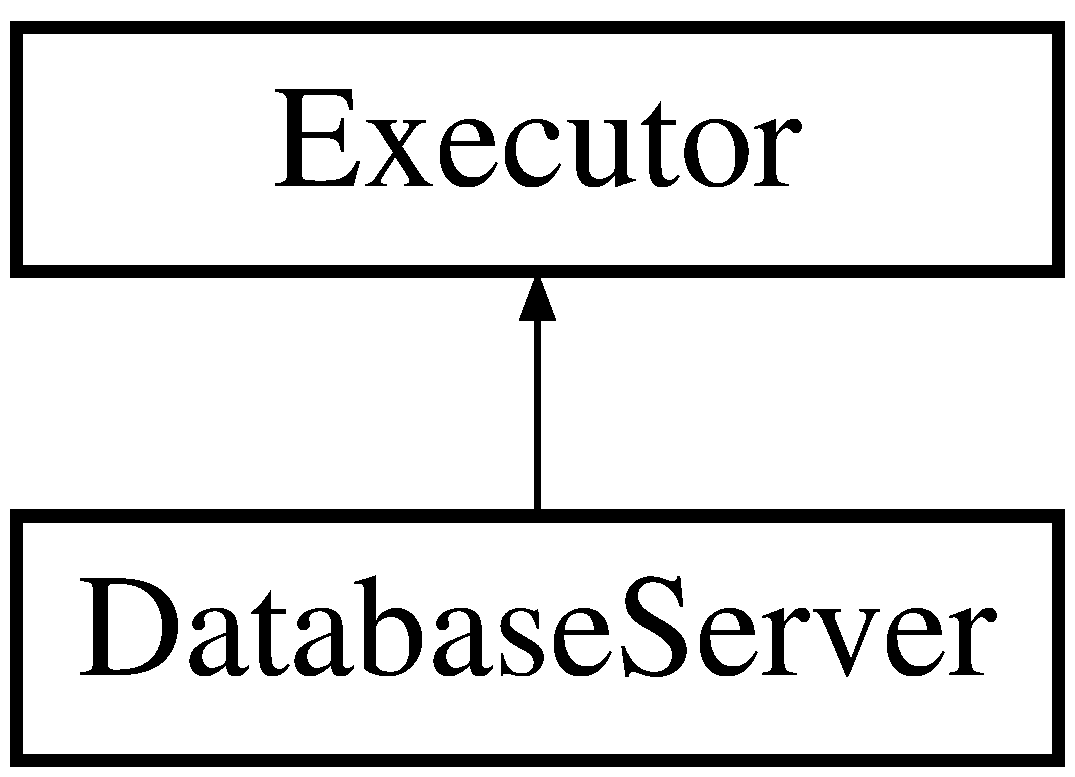
\includegraphics[height=2.000000cm]{class_database_server}
\end{center}
\end{figure}
\subsection*{Public Member Functions}
\begin{DoxyCompactItemize}
\item 
\hyperlink{class_database_server_a47a93c980abf65f1e440a6850ee923f9}{Database\+Server} (int \hyperlink{class_executor_a33c24e2887b4d9c4ef7f3566d3bc803e}{rank}, int \hyperlink{class_executor_a4e798bde66d26fe200de7e8d2b54e915}{number\+\_\+of\+\_\+processors})
\item 
\hyperlink{class_database_server_a36ff1397d646b4672e2aec7ccb102044}{$\sim$\+Database\+Server} ()
\item 
void \hyperlink{class_database_server_af476941a81155fd24d88d3e941be935b}{execute} (int argc, char $\ast$argv\mbox{[}$\,$\mbox{]})
\item 
void \hyperlink{class_database_server_a31064a18819c201d37882c74b25f8cf6}{init\+Database} ()
\end{DoxyCompactItemize}
\subsection*{Additional Inherited Members}


\subsection{Detailed Description}


Definition at line 7 of file Database\+Server.\+h.



\subsection{Constructor \& Destructor Documentation}
\hypertarget{class_database_server_a47a93c980abf65f1e440a6850ee923f9}{}\index{Database\+Server@{Database\+Server}!Database\+Server@{Database\+Server}}
\index{Database\+Server@{Database\+Server}!Database\+Server@{Database\+Server}}
\subsubsection[{Database\+Server}]{\setlength{\rightskip}{0pt plus 5cm}Database\+Server\+::\+Database\+Server (
\begin{DoxyParamCaption}
\item[{int}]{rank, }
\item[{int}]{number\+\_\+of\+\_\+processors}
\end{DoxyParamCaption}
)}\label{class_database_server_a47a93c980abf65f1e440a6850ee923f9}


Definition at line 10 of file Database\+Server.\+cpp.

\hypertarget{class_database_server_a36ff1397d646b4672e2aec7ccb102044}{}\index{Database\+Server@{Database\+Server}!````~Database\+Server@{$\sim$\+Database\+Server}}
\index{````~Database\+Server@{$\sim$\+Database\+Server}!Database\+Server@{Database\+Server}}
\subsubsection[{$\sim$\+Database\+Server}]{\setlength{\rightskip}{0pt plus 5cm}Database\+Server\+::$\sim$\+Database\+Server (
\begin{DoxyParamCaption}
{}
\end{DoxyParamCaption}
)}\label{class_database_server_a36ff1397d646b4672e2aec7ccb102044}


Definition at line 15 of file Database\+Server.\+cpp.



\subsection{Member Function Documentation}
\hypertarget{class_database_server_af476941a81155fd24d88d3e941be935b}{}\index{Database\+Server@{Database\+Server}!execute@{execute}}
\index{execute@{execute}!Database\+Server@{Database\+Server}}
\subsubsection[{execute}]{\setlength{\rightskip}{0pt plus 5cm}void Database\+Server\+::execute (
\begin{DoxyParamCaption}
\item[{int}]{argc, }
\item[{char $\ast$}]{argv\mbox{[}$\,$\mbox{]}}
\end{DoxyParamCaption}
)\hspace{0.3cm}{\ttfamily [virtual]}}\label{class_database_server_af476941a81155fd24d88d3e941be935b}
This procedure is called on all executor subtypes to start them


\begin{DoxyParams}{Parameters}
{\em argc} & command line argument count \\
\hline
{\em argv} & command line arguments \\
\hline
\end{DoxyParams}


Implements \hyperlink{class_executor_aabad4923751a6ea70ca536d4d1f2f32a}{Executor}.



Definition at line 21 of file Database\+Server.\+cpp.

\hypertarget{class_database_server_a31064a18819c201d37882c74b25f8cf6}{}\index{Database\+Server@{Database\+Server}!init\+Database@{init\+Database}}
\index{init\+Database@{init\+Database}!Database\+Server@{Database\+Server}}
\subsubsection[{init\+Database}]{\setlength{\rightskip}{0pt plus 5cm}void Database\+Server\+::init\+Database (
\begin{DoxyParamCaption}
{}
\end{DoxyParamCaption}
)}\label{class_database_server_a31064a18819c201d37882c74b25f8cf6}


The documentation for this class was generated from the following files\+:\begin{DoxyCompactItemize}
\item 
src/database/\hyperlink{_database_server_8h}{Database\+Server.\+h}\item 
src/database/\hyperlink{_database_server_8cpp}{Database\+Server.\+cpp}\end{DoxyCompactItemize}

\hypertarget{class_data_mining}{}\section{Data\+Mining Class Reference}
\label{class_data_mining}\index{Data\+Mining@{Data\+Mining}}


{\ttfamily \#include $<$Data\+Mining.\+h$>$}

Inheritance diagram for Data\+Mining\+:\begin{figure}[H]
\begin{center}
\leavevmode
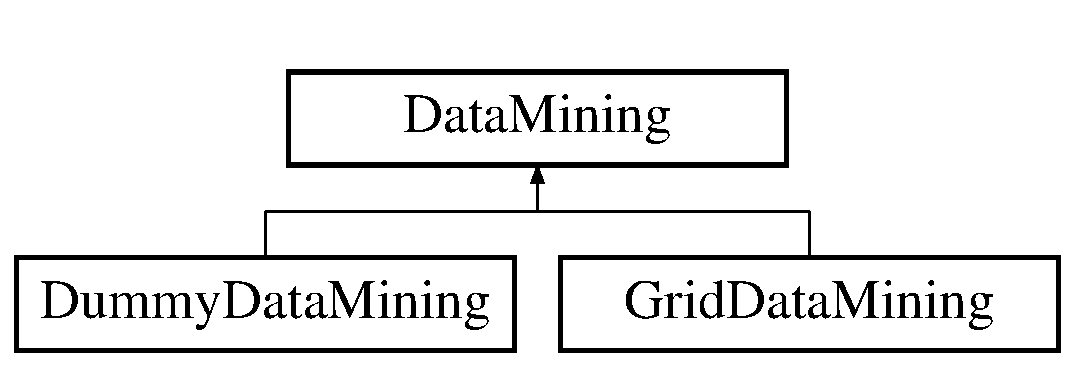
\includegraphics[height=2.000000cm]{class_data_mining}
\end{center}
\end{figure}
\subsection*{Public Member Functions}
\begin{DoxyCompactItemize}
\item 
virtual long \hyperlink{class_data_mining_a03b115a9db40dde60012bde4e4491966}{predict} (double $\ast$parameters)=0
\item 
virtual void \hyperlink{class_data_mining_ae4a8f82a2356d0b45d0e3c750a67aa5c}{insert} (double $\ast$parameters, long runtime)=0
\item 
virtual void \hyperlink{class_data_mining_af47d73e2d04363b1ae22af4db86e5f2e}{init} (int rank, int target\+\_\+rank, int number\+\_\+of\+\_\+important\+\_\+parameters)=0
\end{DoxyCompactItemize}


\subsection{Detailed Description}
Project Dynamic Scheduler for Scientific Simulations 

Definition at line 11 of file Data\+Mining.\+h.



\subsection{Member Function Documentation}
\hypertarget{class_data_mining_af47d73e2d04363b1ae22af4db86e5f2e}{}\index{Data\+Mining@{Data\+Mining}!init@{init}}
\index{init@{init}!Data\+Mining@{Data\+Mining}}
\subsubsection[{init}]{\setlength{\rightskip}{0pt plus 5cm}virtual void Data\+Mining\+::init (
\begin{DoxyParamCaption}
\item[{int}]{rank, }
\item[{int}]{target\+\_\+rank, }
\item[{int}]{number\+\_\+of\+\_\+important\+\_\+parameters}
\end{DoxyParamCaption}
)\hspace{0.3cm}{\ttfamily [pure virtual]}}\label{class_data_mining_af47d73e2d04363b1ae22af4db86e5f2e}
\hypertarget{class_data_mining_ae4a8f82a2356d0b45d0e3c750a67aa5c}{}\index{Data\+Mining@{Data\+Mining}!insert@{insert}}
\index{insert@{insert}!Data\+Mining@{Data\+Mining}}
\subsubsection[{insert}]{\setlength{\rightskip}{0pt plus 5cm}virtual void Data\+Mining\+::insert (
\begin{DoxyParamCaption}
\item[{double $\ast$}]{parameters, }
\item[{long}]{runtime}
\end{DoxyParamCaption}
)\hspace{0.3cm}{\ttfamily [pure virtual]}}\label{class_data_mining_ae4a8f82a2356d0b45d0e3c750a67aa5c}


Implemented in \hyperlink{class_grid_data_mining_a864374110fb8c1673c057f524776ff97}{Grid\+Data\+Mining}.

\hypertarget{class_data_mining_a03b115a9db40dde60012bde4e4491966}{}\index{Data\+Mining@{Data\+Mining}!predict@{predict}}
\index{predict@{predict}!Data\+Mining@{Data\+Mining}}
\subsubsection[{predict}]{\setlength{\rightskip}{0pt plus 5cm}virtual long Data\+Mining\+::predict (
\begin{DoxyParamCaption}
\item[{double $\ast$}]{parameters}
\end{DoxyParamCaption}
)\hspace{0.3cm}{\ttfamily [pure virtual]}}\label{class_data_mining_a03b115a9db40dde60012bde4e4491966}


Implemented in \hyperlink{class_grid_data_mining_a8aef1fbc6d1f034660efee2878f2efe2}{Grid\+Data\+Mining}.



The documentation for this class was generated from the following file\+:\begin{DoxyCompactItemize}
\item 
src/datamining/\hyperlink{_data_mining_8h}{Data\+Mining.\+h}\end{DoxyCompactItemize}

\hypertarget{classel_1_1base_1_1utils_1_1_date_time}{}\section{el\+:\+:base\+:\+:utils\+:\+:Date\+Time Class Reference}
\label{classel_1_1base_1_1utils_1_1_date_time}\index{el\+::base\+::utils\+::\+Date\+Time@{el\+::base\+::utils\+::\+Date\+Time}}


Contains utilities for cross-\/platform date/time. This class make use of \hyperlink{classel_1_1base_1_1utils_1_1_str}{el\+::base\+::utils\+::\+Str}.  




{\ttfamily \#include $<$easylogging++.\+h$>$}

Inheritance diagram for el\+:\+:base\+:\+:utils\+:\+:Date\+Time\+:\begin{figure}[H]
\begin{center}
\leavevmode
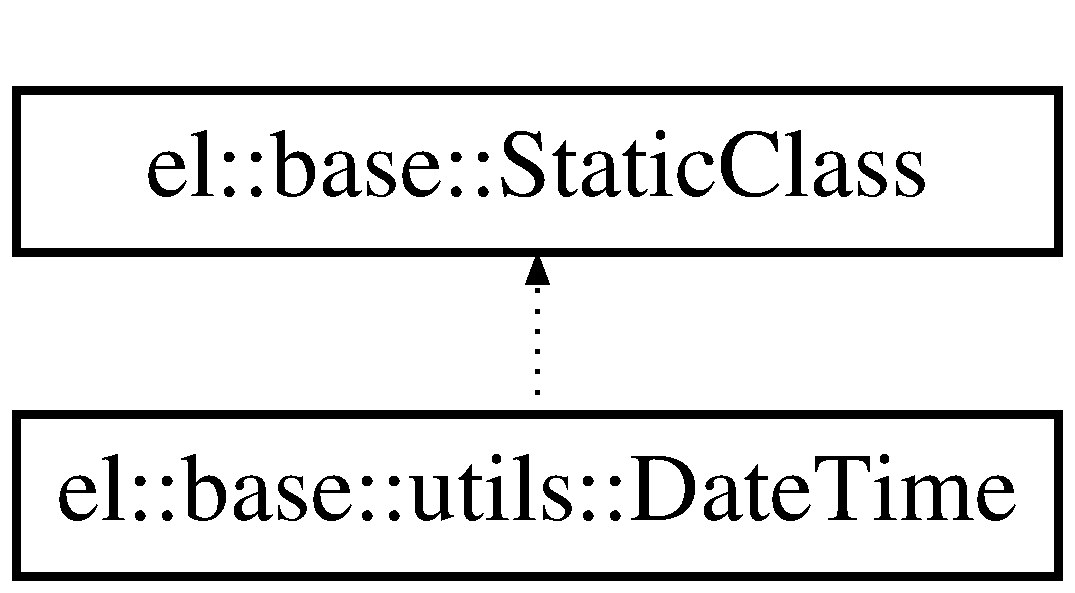
\includegraphics[height=2.000000cm]{classel_1_1base_1_1utils_1_1_date_time}
\end{center}
\end{figure}
\subsection*{Static Public Member Functions}
\begin{DoxyCompactItemize}
\item 
static void \hyperlink{classel_1_1base_1_1utils_1_1_date_time_ac000e6ecf705c2194a173d618ff4acfd}{gettimeofday} (struct timeval $\ast$tv)
\begin{DoxyCompactList}\small\item\em Cross platform gettimeofday for Windows and unix platform. This can be used to determine current millisecond. \end{DoxyCompactList}\item 
static std\+::string \hyperlink{classel_1_1base_1_1utils_1_1_date_time_aa813c606a98b8741f59ccdf5aacef733}{get\+Date\+Time} (const char $\ast$format, const \hyperlink{classel_1_1base_1_1_milliseconds_width}{base\+::\+Milliseconds\+Width} $\ast$ms\+Width)
\begin{DoxyCompactList}\small\item\em Gets current date and time with milliseconds. \end{DoxyCompactList}\item 
static \hyperlink{namespaceel_1_1base_1_1type_a67e406cd213c231f1d135b5a4eda64b5}{base\+::type\+::string\+\_\+t} \hyperlink{classel_1_1base_1_1utils_1_1_date_time_a1eea58fffe291c969a526d08515d29d7}{format\+Time} (unsigned long long time, \hyperlink{namespaceel_1_1base_a1b886858c6409097395b24b1bdf03c39}{base\+::\+Timestamp\+Unit} timestamp\+Unit)
\begin{DoxyCompactList}\small\item\em Formats time to get unit accordingly, units like second if $>$ 1000 or minutes if $>$ 60000 etc. \end{DoxyCompactList}\item 
static unsigned long long \hyperlink{classel_1_1base_1_1utils_1_1_date_time_a9181a3544442e1d3c05d8c96bbfff16d}{get\+Time\+Difference} (const struct timeval \&end\+Time, const struct timeval \&start\+Time, \hyperlink{namespaceel_1_1base_a1b886858c6409097395b24b1bdf03c39}{base\+::\+Timestamp\+Unit} timestamp\+Unit)
\begin{DoxyCompactList}\small\item\em Gets time difference in milli/micro second depending on timestamp\+Unit. \end{DoxyCompactList}\end{DoxyCompactItemize}


\subsection{Detailed Description}
Contains utilities for cross-\/platform date/time. This class make use of \hyperlink{classel_1_1base_1_1utils_1_1_str}{el\+::base\+::utils\+::\+Str}. 

Definition at line 1562 of file easylogging++.\+h.



\subsection{Member Function Documentation}
\hypertarget{classel_1_1base_1_1utils_1_1_date_time_a1eea58fffe291c969a526d08515d29d7}{}\index{el\+::base\+::utils\+::\+Date\+Time@{el\+::base\+::utils\+::\+Date\+Time}!format\+Time@{format\+Time}}
\index{format\+Time@{format\+Time}!el\+::base\+::utils\+::\+Date\+Time@{el\+::base\+::utils\+::\+Date\+Time}}
\subsubsection[{format\+Time}]{\setlength{\rightskip}{0pt plus 5cm}static {\bf base\+::type\+::string\+\_\+t} el\+::base\+::utils\+::\+Date\+Time\+::format\+Time (
\begin{DoxyParamCaption}
\item[{unsigned long long}]{time, }
\item[{{\bf base\+::\+Timestamp\+Unit}}]{timestamp\+Unit}
\end{DoxyParamCaption}
)\hspace{0.3cm}{\ttfamily [inline]}, {\ttfamily [static]}}\label{classel_1_1base_1_1utils_1_1_date_time_a1eea58fffe291c969a526d08515d29d7}


Formats time to get unit accordingly, units like second if $>$ 1000 or minutes if $>$ 60000 etc. 



Definition at line 1611 of file easylogging++.\+h.

\hypertarget{classel_1_1base_1_1utils_1_1_date_time_aa813c606a98b8741f59ccdf5aacef733}{}\index{el\+::base\+::utils\+::\+Date\+Time@{el\+::base\+::utils\+::\+Date\+Time}!get\+Date\+Time@{get\+Date\+Time}}
\index{get\+Date\+Time@{get\+Date\+Time}!el\+::base\+::utils\+::\+Date\+Time@{el\+::base\+::utils\+::\+Date\+Time}}
\subsubsection[{get\+Date\+Time}]{\setlength{\rightskip}{0pt plus 5cm}static std\+::string el\+::base\+::utils\+::\+Date\+Time\+::get\+Date\+Time (
\begin{DoxyParamCaption}
\item[{const char $\ast$}]{format, }
\item[{const {\bf base\+::\+Milliseconds\+Width} $\ast$}]{ms\+Width}
\end{DoxyParamCaption}
)\hspace{0.3cm}{\ttfamily [inline]}, {\ttfamily [static]}}\label{classel_1_1base_1_1utils_1_1_date_time_aa813c606a98b8741f59ccdf5aacef733}


Gets current date and time with milliseconds. 


\begin{DoxyParams}{Parameters}
{\em format} & User provided date/time format \\
\hline
{\em ms\+Width} & A pointer to \hyperlink{classel_1_1base_1_1_milliseconds_width}{base\+::\+Milliseconds\+Width} from configuration (non-\/null) \\
\hline
\end{DoxyParams}
\begin{DoxyReturn}{Returns}
string based date time in specified format. 
\end{DoxyReturn}


Definition at line 1599 of file easylogging++.\+h.

\hypertarget{classel_1_1base_1_1utils_1_1_date_time_a9181a3544442e1d3c05d8c96bbfff16d}{}\index{el\+::base\+::utils\+::\+Date\+Time@{el\+::base\+::utils\+::\+Date\+Time}!get\+Time\+Difference@{get\+Time\+Difference}}
\index{get\+Time\+Difference@{get\+Time\+Difference}!el\+::base\+::utils\+::\+Date\+Time@{el\+::base\+::utils\+::\+Date\+Time}}
\subsubsection[{get\+Time\+Difference}]{\setlength{\rightskip}{0pt plus 5cm}static unsigned long long el\+::base\+::utils\+::\+Date\+Time\+::get\+Time\+Difference (
\begin{DoxyParamCaption}
\item[{const struct timeval \&}]{end\+Time, }
\item[{const struct timeval \&}]{start\+Time, }
\item[{{\bf base\+::\+Timestamp\+Unit}}]{timestamp\+Unit}
\end{DoxyParamCaption}
)\hspace{0.3cm}{\ttfamily [inline]}, {\ttfamily [static]}}\label{classel_1_1base_1_1utils_1_1_date_time_a9181a3544442e1d3c05d8c96bbfff16d}


Gets time difference in milli/micro second depending on timestamp\+Unit. 



Definition at line 1628 of file easylogging++.\+h.

\hypertarget{classel_1_1base_1_1utils_1_1_date_time_ac000e6ecf705c2194a173d618ff4acfd}{}\index{el\+::base\+::utils\+::\+Date\+Time@{el\+::base\+::utils\+::\+Date\+Time}!gettimeofday@{gettimeofday}}
\index{gettimeofday@{gettimeofday}!el\+::base\+::utils\+::\+Date\+Time@{el\+::base\+::utils\+::\+Date\+Time}}
\subsubsection[{gettimeofday}]{\setlength{\rightskip}{0pt plus 5cm}static void el\+::base\+::utils\+::\+Date\+Time\+::gettimeofday (
\begin{DoxyParamCaption}
\item[{struct timeval $\ast$}]{tv}
\end{DoxyParamCaption}
)\hspace{0.3cm}{\ttfamily [inline]}, {\ttfamily [static]}}\label{classel_1_1base_1_1utils_1_1_date_time_ac000e6ecf705c2194a173d618ff4acfd}


Cross platform gettimeofday for Windows and unix platform. This can be used to determine current millisecond. 

For unix system it uses gettimeofday(timeval$\ast$, timezone$\ast$) and for Windows, a seperate implementation is provided 
\begin{DoxyParams}[1]{Parameters}
\mbox{\tt in,out}  & {\em tv} & Pointer that gets updated \\
\hline
\end{DoxyParams}


Definition at line 1568 of file easylogging++.\+h.



The documentation for this class was generated from the following file\+:\begin{DoxyCompactItemize}
\item 
lib/\hyperlink{easylogging_09_09_8h}{easylogging++.\+h}\end{DoxyCompactItemize}

\hypertarget{classel_1_1base_1_1_default_log_builder}{}\section{el\+:\+:base\+:\+:Default\+Log\+Builder Class Reference}
\label{classel_1_1base_1_1_default_log_builder}\index{el\+::base\+::\+Default\+Log\+Builder@{el\+::base\+::\+Default\+Log\+Builder}}


{\ttfamily \#include $<$easylogging++.\+h$>$}

Inheritance diagram for el\+:\+:base\+:\+:Default\+Log\+Builder\+:\begin{figure}[H]
\begin{center}
\leavevmode
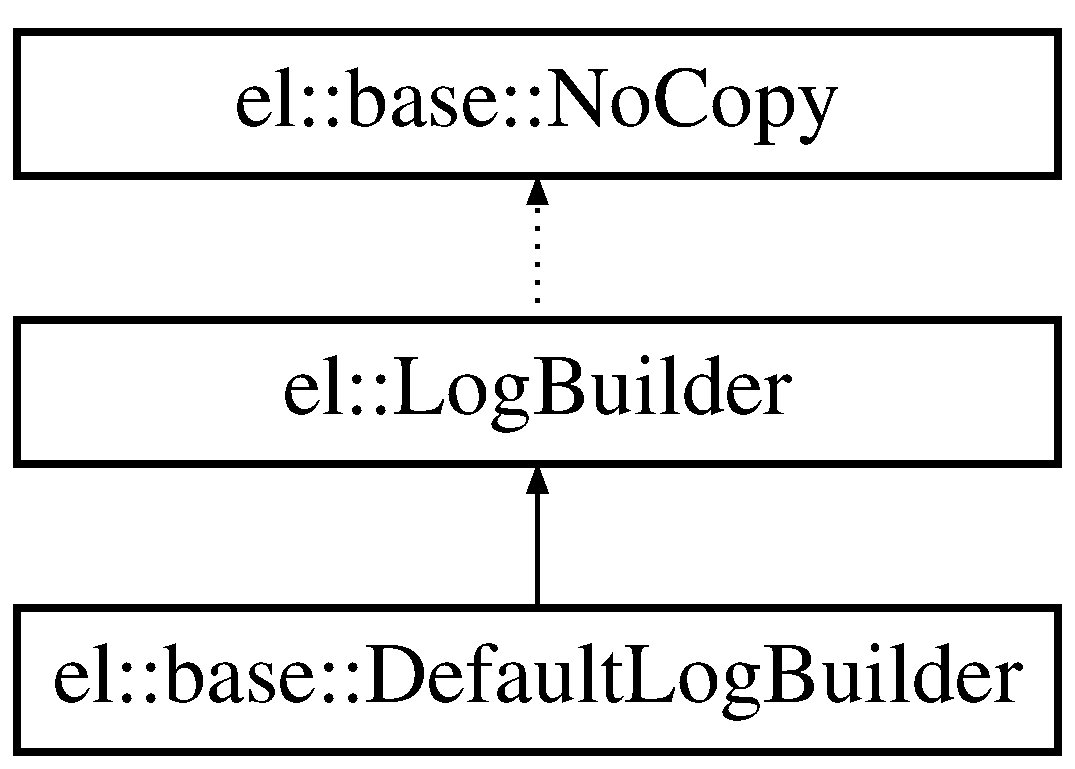
\includegraphics[height=3.000000cm]{classel_1_1base_1_1_default_log_builder}
\end{center}
\end{figure}
\subsection*{Public Member Functions}
\begin{DoxyCompactItemize}
\item 
\hyperlink{namespaceel_1_1base_1_1type_a67e406cd213c231f1d135b5a4eda64b5}{base\+::type\+::string\+\_\+t} \hyperlink{classel_1_1base_1_1_default_log_builder_aa8d2f42068115d899ed81de1b0ed360e}{build} (const \hyperlink{classel_1_1_log_message}{Log\+Message} $\ast$log\+Message, bool append\+New\+Line) const 
\end{DoxyCompactItemize}


\subsection{Detailed Description}


Definition at line 4367 of file easylogging++.\+h.



\subsection{Member Function Documentation}
\hypertarget{classel_1_1base_1_1_default_log_builder_aa8d2f42068115d899ed81de1b0ed360e}{}\index{el\+::base\+::\+Default\+Log\+Builder@{el\+::base\+::\+Default\+Log\+Builder}!build@{build}}
\index{build@{build}!el\+::base\+::\+Default\+Log\+Builder@{el\+::base\+::\+Default\+Log\+Builder}}
\subsubsection[{build}]{\setlength{\rightskip}{0pt plus 5cm}{\bf base\+::type\+::string\+\_\+t} el\+::base\+::\+Default\+Log\+Builder\+::build (
\begin{DoxyParamCaption}
\item[{const {\bf Log\+Message} $\ast$}]{log\+Message, }
\item[{bool}]{append\+New\+Line}
\end{DoxyParamCaption}
) const\hspace{0.3cm}{\ttfamily [inline]}, {\ttfamily [virtual]}}\label{classel_1_1base_1_1_default_log_builder_aa8d2f42068115d899ed81de1b0ed360e}


Implements \hyperlink{classel_1_1_log_builder_a633b373a3bb9d3e17bdd664aeba4dbc8}{el\+::\+Log\+Builder}.



Definition at line 4369 of file easylogging++.\+h.



The documentation for this class was generated from the following file\+:\begin{DoxyCompactItemize}
\item 
lib/\hyperlink{easylogging_09_09_8h}{easylogging++.\+h}\end{DoxyCompactItemize}

\hypertarget{classel_1_1base_1_1_default_log_dispatch_callback}{}\section{el\+:\+:base\+:\+:Default\+Log\+Dispatch\+Callback Class Reference}
\label{classel_1_1base_1_1_default_log_dispatch_callback}\index{el\+::base\+::\+Default\+Log\+Dispatch\+Callback@{el\+::base\+::\+Default\+Log\+Dispatch\+Callback}}


{\ttfamily \#include $<$easylogging++.\+h$>$}

Inheritance diagram for el\+:\+:base\+:\+:Default\+Log\+Dispatch\+Callback\+:\begin{figure}[H]
\begin{center}
\leavevmode
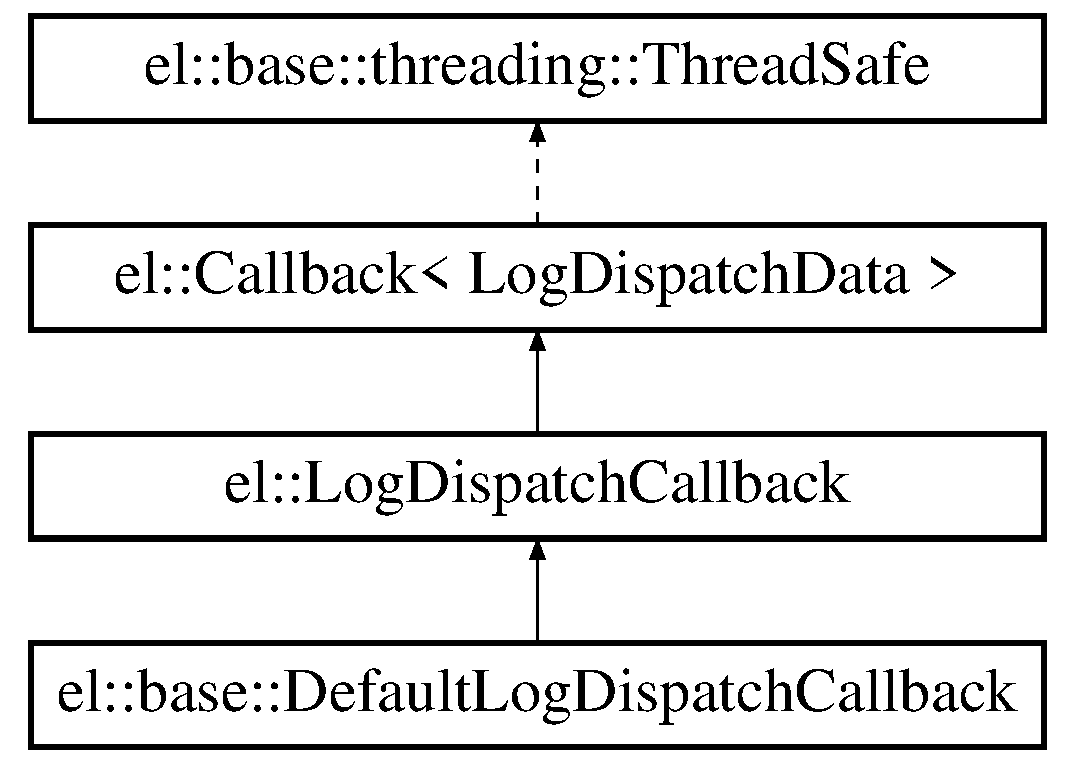
\includegraphics[height=4.000000cm]{classel_1_1base_1_1_default_log_dispatch_callback}
\end{center}
\end{figure}
\subsection*{Protected Member Functions}
\begin{DoxyCompactItemize}
\item 
void \hyperlink{classel_1_1base_1_1_default_log_dispatch_callback_acdac30f202c245500e6d94c55eee6d95}{handle} (const \hyperlink{classel_1_1_log_dispatch_data}{Log\+Dispatch\+Data} $\ast$data)
\end{DoxyCompactItemize}
\subsection*{Additional Inherited Members}


\subsection{Detailed Description}


Definition at line 4168 of file easylogging++.\+h.



\subsection{Member Function Documentation}
\hypertarget{classel_1_1base_1_1_default_log_dispatch_callback_acdac30f202c245500e6d94c55eee6d95}{}\index{el\+::base\+::\+Default\+Log\+Dispatch\+Callback@{el\+::base\+::\+Default\+Log\+Dispatch\+Callback}!handle@{handle}}
\index{handle@{handle}!el\+::base\+::\+Default\+Log\+Dispatch\+Callback@{el\+::base\+::\+Default\+Log\+Dispatch\+Callback}}
\subsubsection[{handle}]{\setlength{\rightskip}{0pt plus 5cm}void el\+::base\+::\+Default\+Log\+Dispatch\+Callback\+::handle (
\begin{DoxyParamCaption}
\item[{const {\bf Log\+Dispatch\+Data} $\ast$}]{data}
\end{DoxyParamCaption}
)\hspace{0.3cm}{\ttfamily [inline]}, {\ttfamily [protected]}, {\ttfamily [virtual]}}\label{classel_1_1base_1_1_default_log_dispatch_callback_acdac30f202c245500e6d94c55eee6d95}


Implements \hyperlink{classel_1_1_callback_a8997c7971d65062c374ef24e653061be}{el\+::\+Callback$<$ Log\+Dispatch\+Data $>$}.



Definition at line 4170 of file easylogging++.\+h.



The documentation for this class was generated from the following file\+:\begin{DoxyCompactItemize}
\item 
lib/\hyperlink{easylogging_09_09_8h}{easylogging++.\+h}\end{DoxyCompactItemize}

\hypertarget{classel_1_1base_1_1_default_performance_tracking_callback}{}\section{el\+:\+:base\+:\+:Default\+Performance\+Tracking\+Callback Class Reference}
\label{classel_1_1base_1_1_default_performance_tracking_callback}\index{el\+::base\+::\+Default\+Performance\+Tracking\+Callback@{el\+::base\+::\+Default\+Performance\+Tracking\+Callback}}


{\ttfamily \#include $<$easylogging++.\+h$>$}

Inheritance diagram for el\+:\+:base\+:\+:Default\+Performance\+Tracking\+Callback\+:\begin{figure}[H]
\begin{center}
\leavevmode
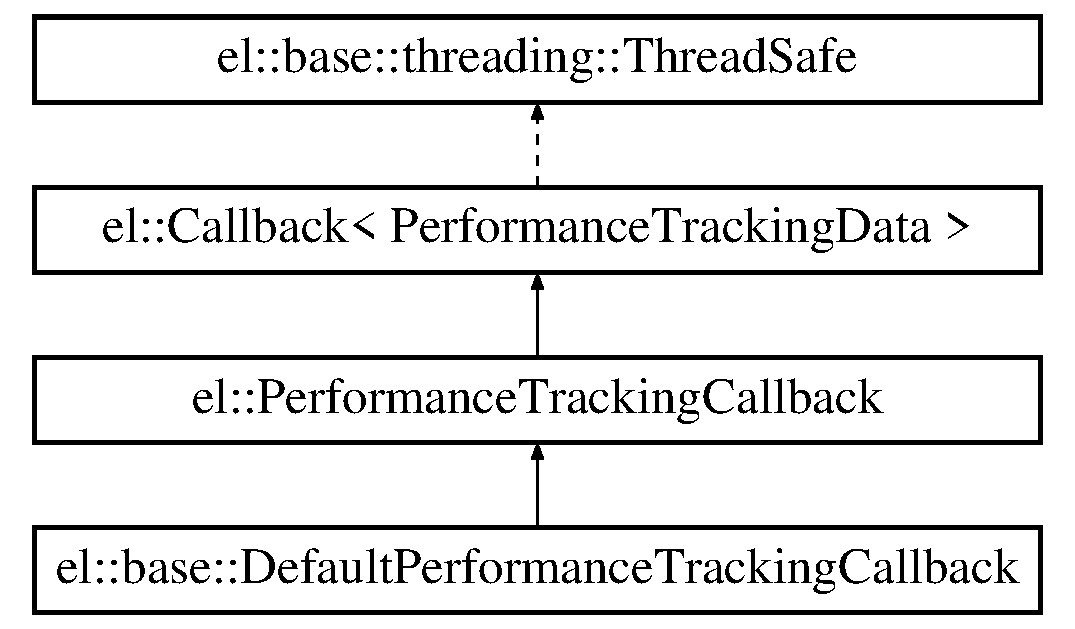
\includegraphics[height=4.000000cm]{classel_1_1base_1_1_default_performance_tracking_callback}
\end{center}
\end{figure}
\subsection*{Protected Member Functions}
\begin{DoxyCompactItemize}
\item 
void \hyperlink{classel_1_1base_1_1_default_performance_tracking_callback_afabb8820e1bd9a7fb89508fe11f59d37}{handle} (const \hyperlink{classel_1_1_performance_tracking_data}{Performance\+Tracking\+Data} $\ast$data)
\end{DoxyCompactItemize}
\subsection*{Additional Inherited Members}


\subsection{Detailed Description}


Definition at line 5397 of file easylogging++.\+h.



\subsection{Member Function Documentation}
\hypertarget{classel_1_1base_1_1_default_performance_tracking_callback_afabb8820e1bd9a7fb89508fe11f59d37}{}\index{el\+::base\+::\+Default\+Performance\+Tracking\+Callback@{el\+::base\+::\+Default\+Performance\+Tracking\+Callback}!handle@{handle}}
\index{handle@{handle}!el\+::base\+::\+Default\+Performance\+Tracking\+Callback@{el\+::base\+::\+Default\+Performance\+Tracking\+Callback}}
\subsubsection[{handle}]{\setlength{\rightskip}{0pt plus 5cm}void el\+::base\+::\+Default\+Performance\+Tracking\+Callback\+::handle (
\begin{DoxyParamCaption}
\item[{const {\bf Performance\+Tracking\+Data} $\ast$}]{data}
\end{DoxyParamCaption}
)\hspace{0.3cm}{\ttfamily [inline]}, {\ttfamily [protected]}, {\ttfamily [virtual]}}\label{classel_1_1base_1_1_default_performance_tracking_callback_afabb8820e1bd9a7fb89508fe11f59d37}


Implements \hyperlink{classel_1_1_callback_a8997c7971d65062c374ef24e653061be}{el\+::\+Callback$<$ Performance\+Tracking\+Data $>$}.



Definition at line 5399 of file easylogging++.\+h.



The documentation for this class was generated from the following file\+:\begin{DoxyCompactItemize}
\item 
lib/\hyperlink{easylogging_09_09_8h}{easylogging++.\+h}\end{DoxyCompactItemize}

\hypertarget{class_dummy_data_mining}{}\section{Dummy\+Data\+Mining Class Reference}
\label{class_dummy_data_mining}\index{Dummy\+Data\+Mining@{Dummy\+Data\+Mining}}


{\ttfamily \#include $<$Dummy\+Data\+Mining.\+h$>$}

Inheritance diagram for Dummy\+Data\+Mining\+:\begin{figure}[H]
\begin{center}
\leavevmode
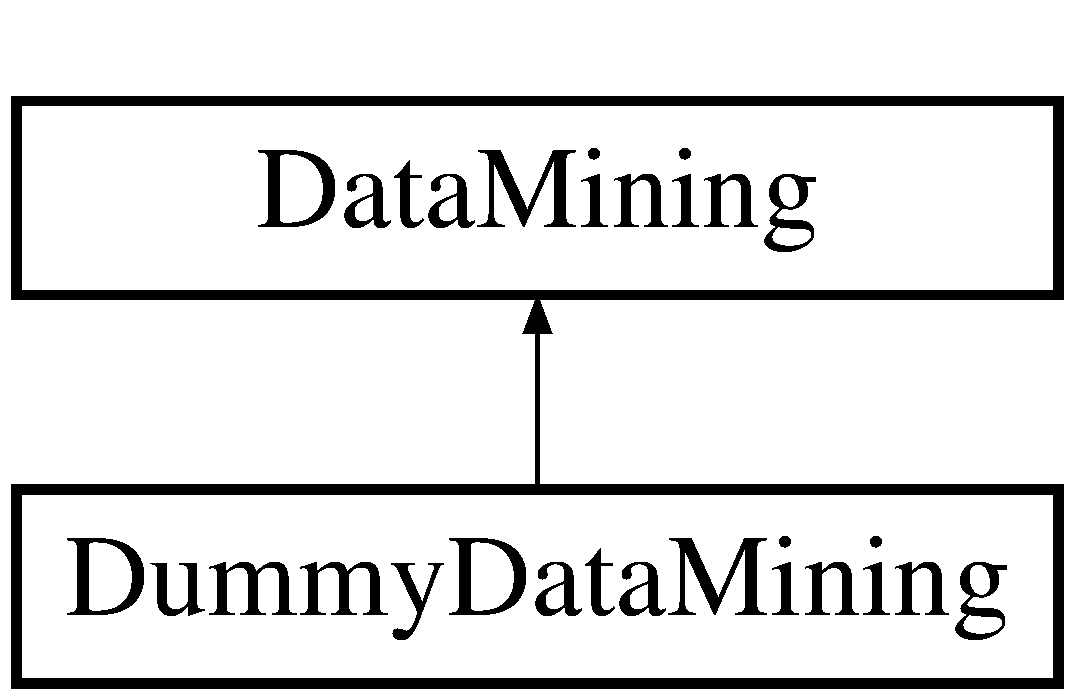
\includegraphics[height=2.000000cm]{class_dummy_data_mining}
\end{center}
\end{figure}
\subsection*{Additional Inherited Members}


\subsection{Detailed Description}


Definition at line 10 of file Dummy\+Data\+Mining.\+h.



The documentation for this class was generated from the following files\+:\begin{DoxyCompactItemize}
\item 
src/datamining/\hyperlink{_dummy_data_mining_8h}{Dummy\+Data\+Mining.\+h}\item 
src/datamining/\hyperlink{_dummy_data_mining_8cpp}{Dummy\+Data\+Mining.\+cpp}\end{DoxyCompactItemize}

\hypertarget{class_executor}{}\section{Executor Class Reference}
\label{class_executor}\index{Executor@{Executor}}


{\ttfamily \#include $<$Executor.\+h$>$}

Inheritance diagram for Executor\+:\begin{figure}[H]
\begin{center}
\leavevmode
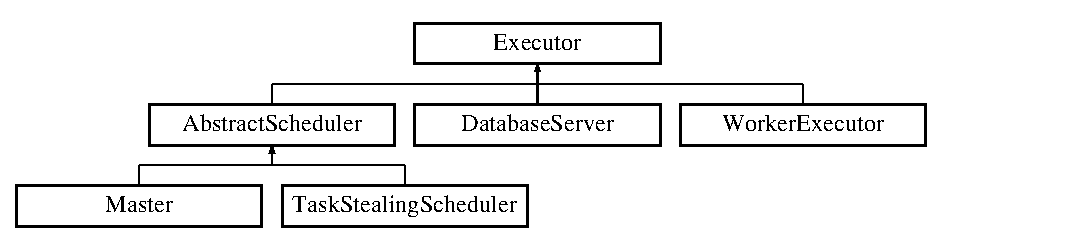
\includegraphics[height=2.818792cm]{class_executor}
\end{center}
\end{figure}
\subsection*{Public Member Functions}
\begin{DoxyCompactItemize}
\item 
\hyperlink{class_executor_ad0a052ec3c021786fed3c8d336ab0659}{Executor} (int \hyperlink{class_executor_a33c24e2887b4d9c4ef7f3566d3bc803e}{rank}, int \hyperlink{class_executor_a4e798bde66d26fe200de7e8d2b54e915}{number\+\_\+of\+\_\+processors})
\item 
virtual \hyperlink{class_executor_a23108c89c4a25e22c927115191c04b26}{$\sim$\+Executor} ()
\item 
virtual void \hyperlink{class_executor_aabad4923751a6ea70ca536d4d1f2f32a}{execute} (int argc, char $\ast$argv\mbox{[}$\,$\mbox{]})=0
\end{DoxyCompactItemize}
\subsection*{Static Public Member Functions}
\begin{DoxyCompactItemize}
\item 
static \hyperlink{class_executor}{Executor} $\ast$ \hyperlink{class_executor_ab193432d6f64407c45780629e3341a87}{get\+\_\+new\+\_\+executor\+\_\+by\+\_\+rank} (int \hyperlink{class_executor_a33c24e2887b4d9c4ef7f3566d3bc803e}{rank}, int \hyperlink{class_executor_a4e798bde66d26fe200de7e8d2b54e915}{number\+\_\+of\+\_\+processors}, \hyperlink{_design_enum_8h_aefcba5d81ba393e442410d16ebe78ac7}{Design\+Enum} design, \hyperlink{_strategy_enum_8h_aa770fe6711c27326278b9e4ab326cd10}{Strategy\+Enum} strategy)
\end{DoxyCompactItemize}
\subsection*{Protected Attributes}
\begin{DoxyCompactItemize}
\item 
const int \hyperlink{class_executor_a33c24e2887b4d9c4ef7f3566d3bc803e}{rank}
\item 
const int \hyperlink{class_executor_a4e798bde66d26fe200de7e8d2b54e915}{number\+\_\+of\+\_\+processors}
\end{DoxyCompactItemize}


\subsection{Detailed Description}
The \hyperlink{class_executor}{Executor} class is the base class for all objects that are mpi processes and have a one mpi rank.

\begin{DoxyAuthor}{Author}
Fabio Broghammer 
\end{DoxyAuthor}
\begin{DoxyVersion}{Version}
1.\+0 
\end{DoxyVersion}


Definition at line 15 of file Executor.\+h.



\subsection{Constructor \& Destructor Documentation}
\hypertarget{class_executor_ad0a052ec3c021786fed3c8d336ab0659}{}\index{Executor@{Executor}!Executor@{Executor}}
\index{Executor@{Executor}!Executor@{Executor}}
\subsubsection[{Executor}]{\setlength{\rightskip}{0pt plus 5cm}Executor\+::\+Executor (
\begin{DoxyParamCaption}
\item[{int}]{rank, }
\item[{int}]{number\+\_\+of\+\_\+processors}
\end{DoxyParamCaption}
)}\label{class_executor_ad0a052ec3c021786fed3c8d336ab0659}
Constructs a new executor object and initialize the parameters rank and number\+\_\+of\+\_\+processors


\begin{DoxyParams}{Parameters}
{\em rank} & the M\+P\+I rank of the processor, that runs the executor code \\
\hline
{\em number\+\_\+of\+\_\+processors} & the total number of processors of the M\+P\+I world \\
\hline
\end{DoxyParams}


Definition at line 17 of file Executor.\+cpp.

\hypertarget{class_executor_a23108c89c4a25e22c927115191c04b26}{}\index{Executor@{Executor}!````~Executor@{$\sim$\+Executor}}
\index{````~Executor@{$\sim$\+Executor}!Executor@{Executor}}
\subsubsection[{$\sim$\+Executor}]{\setlength{\rightskip}{0pt plus 5cm}Executor\+::$\sim$\+Executor (
\begin{DoxyParamCaption}
{}
\end{DoxyParamCaption}
)\hspace{0.3cm}{\ttfamily [virtual]}}\label{class_executor_a23108c89c4a25e22c927115191c04b26}


Definition at line 23 of file Executor.\+cpp.



\subsection{Member Function Documentation}
\hypertarget{class_executor_aabad4923751a6ea70ca536d4d1f2f32a}{}\index{Executor@{Executor}!execute@{execute}}
\index{execute@{execute}!Executor@{Executor}}
\subsubsection[{execute}]{\setlength{\rightskip}{0pt plus 5cm}virtual void Executor\+::execute (
\begin{DoxyParamCaption}
\item[{int}]{argc, }
\item[{char $\ast$}]{argv\mbox{[}$\,$\mbox{]}}
\end{DoxyParamCaption}
)\hspace{0.3cm}{\ttfamily [pure virtual]}}\label{class_executor_aabad4923751a6ea70ca536d4d1f2f32a}
This procedure is called on all executor subtypes to start them


\begin{DoxyParams}{Parameters}
{\em argc} & command line argument count \\
\hline
{\em argv} & command line arguments \\
\hline
\end{DoxyParams}


Implemented in \hyperlink{class_master_acea94dce898273bbbddfaae52f243bca}{Master}, \hyperlink{class_worker_executor_adb37338d137f4039d835519b14698d51}{Worker\+Executor}, \hyperlink{class_task_stealing_scheduler_a8e2a2515ccc6021980508ba085f104fa}{Task\+Stealing\+Scheduler}, and \hyperlink{class_database_server_af476941a81155fd24d88d3e941be935b}{Database\+Server}.

\hypertarget{class_executor_ab193432d6f64407c45780629e3341a87}{}\index{Executor@{Executor}!get\+\_\+new\+\_\+executor\+\_\+by\+\_\+rank@{get\+\_\+new\+\_\+executor\+\_\+by\+\_\+rank}}
\index{get\+\_\+new\+\_\+executor\+\_\+by\+\_\+rank@{get\+\_\+new\+\_\+executor\+\_\+by\+\_\+rank}!Executor@{Executor}}
\subsubsection[{get\+\_\+new\+\_\+executor\+\_\+by\+\_\+rank}]{\setlength{\rightskip}{0pt plus 5cm}{\bf Executor} $\ast$ Executor\+::get\+\_\+new\+\_\+executor\+\_\+by\+\_\+rank (
\begin{DoxyParamCaption}
\item[{int}]{rank, }
\item[{int}]{number\+\_\+of\+\_\+processors, }
\item[{{\bf Design\+Enum}}]{design, }
\item[{{\bf Strategy\+Enum}}]{strategy}
\end{DoxyParamCaption}
)\hspace{0.3cm}{\ttfamily [static]}}\label{class_executor_ab193432d6f64407c45780629e3341a87}
Returns a executor instance depending on the rank and design


\begin{DoxyParams}{Parameters}
{\em rank} & of the process \\
\hline
{\em number\+\_\+of\+\_\+processors} & of the M\+P\+I\+\_\+\+C\+O\+M\+M\+\_\+\+W\+O\+R\+L\+D communicator \\
\hline
{\em design} & to be used \\
\hline
{\em strategy} & to be used\\
\hline
\end{DoxyParams}
\begin{DoxyReturn}{Returns}
a executor object 
\end{DoxyReturn}


Definition at line 25 of file Executor.\+cpp.



\subsection{Member Data Documentation}
\hypertarget{class_executor_a4e798bde66d26fe200de7e8d2b54e915}{}\index{Executor@{Executor}!number\+\_\+of\+\_\+processors@{number\+\_\+of\+\_\+processors}}
\index{number\+\_\+of\+\_\+processors@{number\+\_\+of\+\_\+processors}!Executor@{Executor}}
\subsubsection[{number\+\_\+of\+\_\+processors}]{\setlength{\rightskip}{0pt plus 5cm}const int Executor\+::number\+\_\+of\+\_\+processors\hspace{0.3cm}{\ttfamily [protected]}}\label{class_executor_a4e798bde66d26fe200de7e8d2b54e915}
The total number of processors of the M\+P\+I world 

Definition at line 24 of file Executor.\+h.

\hypertarget{class_executor_a33c24e2887b4d9c4ef7f3566d3bc803e}{}\index{Executor@{Executor}!rank@{rank}}
\index{rank@{rank}!Executor@{Executor}}
\subsubsection[{rank}]{\setlength{\rightskip}{0pt plus 5cm}const int Executor\+::rank\hspace{0.3cm}{\ttfamily [protected]}}\label{class_executor_a33c24e2887b4d9c4ef7f3566d3bc803e}
The M\+P\+I rank of the processor, that runs the executor code 

Definition at line 20 of file Executor.\+h.



The documentation for this class was generated from the following files\+:\begin{DoxyCompactItemize}
\item 
src/\hyperlink{_executor_8h}{Executor.\+h}\item 
src/\hyperlink{_executor_8cpp}{Executor.\+cpp}\end{DoxyCompactItemize}

\hypertarget{class_f_i_f_o}{}\section{F\+I\+F\+O Class Reference}
\label{class_f_i_f_o}\index{F\+I\+F\+O@{F\+I\+F\+O}}


{\ttfamily \#include $<$F\+I\+F\+O.\+h$>$}

Inheritance diagram for F\+I\+F\+O\+:\begin{figure}[H]
\begin{center}
\leavevmode
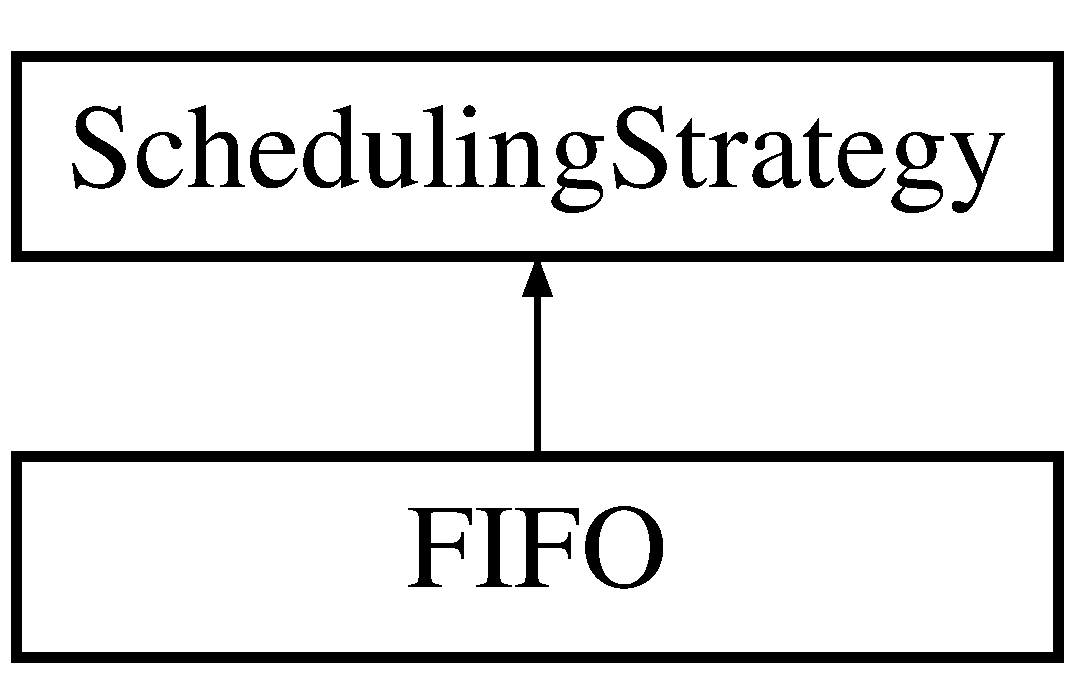
\includegraphics[height=2.000000cm]{class_f_i_f_o}
\end{center}
\end{figure}
\subsection*{Public Member Functions}
\begin{DoxyCompactItemize}
\item 
\hyperlink{class_f_i_f_o_aea969385961885a8e70732482d64fead}{F\+I\+F\+O} ()
\item 
\hyperlink{class_f_i_f_o_a44d31a29b91fed5e154f26bf9df4d280}{$\sim$\+F\+I\+F\+O} ()
\item 
\hyperlink{_types_8h_a0c77930ab3818a1680c59353f627fba8}{Task} \hyperlink{class_f_i_f_o_a4f1234aa7afcd3017a7e0470a63a28c7}{get\+\_\+next\+\_\+task} ()
\item 
int \hyperlink{class_f_i_f_o_a4a03d69c49827b555a4968733195fd01}{get\+\_\+task\+\_\+count} ()
\item 
\hyperlink{_types_8h_a0c77930ab3818a1680c59353f627fba8}{Task} \hyperlink{class_f_i_f_o_aa96d491319ffa72dbb923693a692ed40}{pop\+\_\+next\+\_\+task} ()
\item 
void \hyperlink{class_f_i_f_o_aa91a84fbe7f8755b4fd7dab27dfd3b72}{push\+\_\+new\+\_\+task} (\hyperlink{_types_8h_a0c77930ab3818a1680c59353f627fba8}{Task} task, long runtime)
\item 
\hyperlink{class_scheduling_strategy}{Scheduling\+Strategy} $\ast$ \hyperlink{class_f_i_f_o_a1f94031b462c35718f2d3ebe16acfa9c}{change\+\_\+strategy} (\hyperlink{class_scheduling_strategy}{Scheduling\+Strategy} $\ast$new\+\_\+strategy)
\item 
bool \hyperlink{class_f_i_f_o_aff0f1a994e551ccfad05e7338652a16d}{is\+\_\+statistic\+\_\+based} ()
\end{DoxyCompactItemize}
\subsection*{Additional Inherited Members}


\subsection{Detailed Description}
This class realize the first in-\/first out (\hyperlink{class_f_i_f_o}{F\+I\+F\+O}) scheduling strategy. The \hyperlink{class_f_i_f_o}{F\+I\+F\+O} class uses the std\+::queue as fifo queue.

\begin{DoxyAuthor}{Author}
Fabio Broghammer 
\end{DoxyAuthor}
\begin{DoxyVersion}{Version}
1.\+0 
\end{DoxyVersion}


Definition at line 16 of file F\+I\+F\+O.\+h.



\subsection{Constructor \& Destructor Documentation}
\hypertarget{class_f_i_f_o_aea969385961885a8e70732482d64fead}{}\index{F\+I\+F\+O@{F\+I\+F\+O}!F\+I\+F\+O@{F\+I\+F\+O}}
\index{F\+I\+F\+O@{F\+I\+F\+O}!F\+I\+F\+O@{F\+I\+F\+O}}
\subsubsection[{F\+I\+F\+O}]{\setlength{\rightskip}{0pt plus 5cm}F\+I\+F\+O\+::\+F\+I\+F\+O (
\begin{DoxyParamCaption}
{}
\end{DoxyParamCaption}
)}\label{class_f_i_f_o_aea969385961885a8e70732482d64fead}
Constructs a new \hyperlink{class_f_i_f_o}{F\+I\+F\+O} scheduling queue 

Definition at line 6 of file F\+I\+F\+O.\+cpp.

\hypertarget{class_f_i_f_o_a44d31a29b91fed5e154f26bf9df4d280}{}\index{F\+I\+F\+O@{F\+I\+F\+O}!````~F\+I\+F\+O@{$\sim$\+F\+I\+F\+O}}
\index{````~F\+I\+F\+O@{$\sim$\+F\+I\+F\+O}!F\+I\+F\+O@{F\+I\+F\+O}}
\subsubsection[{$\sim$\+F\+I\+F\+O}]{\setlength{\rightskip}{0pt plus 5cm}F\+I\+F\+O\+::$\sim$\+F\+I\+F\+O (
\begin{DoxyParamCaption}
{}
\end{DoxyParamCaption}
)}\label{class_f_i_f_o_a44d31a29b91fed5e154f26bf9df4d280}
Destructs a new \hyperlink{class_f_i_f_o}{F\+I\+F\+O} scheduling queue 

Definition at line 11 of file F\+I\+F\+O.\+cpp.



\subsection{Member Function Documentation}
\hypertarget{class_f_i_f_o_a1f94031b462c35718f2d3ebe16acfa9c}{}\index{F\+I\+F\+O@{F\+I\+F\+O}!change\+\_\+strategy@{change\+\_\+strategy}}
\index{change\+\_\+strategy@{change\+\_\+strategy}!F\+I\+F\+O@{F\+I\+F\+O}}
\subsubsection[{change\+\_\+strategy}]{\setlength{\rightskip}{0pt plus 5cm}{\bf Scheduling\+Strategy} $\ast$ F\+I\+F\+O\+::change\+\_\+strategy (
\begin{DoxyParamCaption}
\item[{{\bf Scheduling\+Strategy} $\ast$}]{new\+\_\+strategy}
\end{DoxyParamCaption}
)\hspace{0.3cm}{\ttfamily [virtual]}}\label{class_f_i_f_o_a1f94031b462c35718f2d3ebe16acfa9c}
Changes the scheduling strategy. Returns the new schdeuling strategy with all tasks, or N\+U\+L\+L if there was an error.

Estimated runtime of tasks will get lost by changing from statistically based strategies (L\+S\+F, \hyperlink{class_s_j_f}{S\+J\+F}) to non-\/statistically based strategies. The order of the old queue will be kept.

All tasks will get a default rumtime value (defined in D\+E\+F\+A\+U\+L\+T\+\_\+\+R\+U\+N\+T\+I\+M\+E) by changing from non-\/statistically based strategies (\hyperlink{class_f_i_f_o}{F\+I\+F\+O}, \hyperlink{class_l_i_f_o}{L\+I\+F\+O}) to statistically based strategies. The order of the old queue perhaps won\textquotesingle{}t be kept 
\begin{DoxyParams}{Parameters}
{\em new\+\_\+strategy} & \\
\hline
\end{DoxyParams}


Implements \hyperlink{class_scheduling_strategy_a4874d194c1bb185480339360fe907d83}{Scheduling\+Strategy}.



Definition at line 39 of file F\+I\+F\+O.\+cpp.

\hypertarget{class_f_i_f_o_a4f1234aa7afcd3017a7e0470a63a28c7}{}\index{F\+I\+F\+O@{F\+I\+F\+O}!get\+\_\+next\+\_\+task@{get\+\_\+next\+\_\+task}}
\index{get\+\_\+next\+\_\+task@{get\+\_\+next\+\_\+task}!F\+I\+F\+O@{F\+I\+F\+O}}
\subsubsection[{get\+\_\+next\+\_\+task}]{\setlength{\rightskip}{0pt plus 5cm}{\bf Task} F\+I\+F\+O\+::get\+\_\+next\+\_\+task (
\begin{DoxyParamCaption}
{}
\end{DoxyParamCaption}
)\hspace{0.3cm}{\ttfamily [virtual]}}\label{class_f_i_f_o_a4f1234aa7afcd3017a7e0470a63a28c7}
Returns the first-\/in task depending, or N\+U\+L\+L if the queue is empty

\begin{DoxyReturn}{Returns}
the first-\/in task 
\end{DoxyReturn}


Implements \hyperlink{class_scheduling_strategy_adce3619801460ad67d6c8f9bdffcd36b}{Scheduling\+Strategy}.



Definition at line 17 of file F\+I\+F\+O.\+cpp.

\hypertarget{class_f_i_f_o_a4a03d69c49827b555a4968733195fd01}{}\index{F\+I\+F\+O@{F\+I\+F\+O}!get\+\_\+task\+\_\+count@{get\+\_\+task\+\_\+count}}
\index{get\+\_\+task\+\_\+count@{get\+\_\+task\+\_\+count}!F\+I\+F\+O@{F\+I\+F\+O}}
\subsubsection[{get\+\_\+task\+\_\+count}]{\setlength{\rightskip}{0pt plus 5cm}int F\+I\+F\+O\+::get\+\_\+task\+\_\+count (
\begin{DoxyParamCaption}
{}
\end{DoxyParamCaption}
)\hspace{0.3cm}{\ttfamily [virtual]}}\label{class_f_i_f_o_a4a03d69c49827b555a4968733195fd01}
Return the count of tasks in the scheduling queue

the count of tasks 

Implements \hyperlink{class_scheduling_strategy_a0a3355ffe9c03236692ad00e4f94f5c5}{Scheduling\+Strategy}.



Definition at line 22 of file F\+I\+F\+O.\+cpp.

\hypertarget{class_f_i_f_o_aff0f1a994e551ccfad05e7338652a16d}{}\index{F\+I\+F\+O@{F\+I\+F\+O}!is\+\_\+statistic\+\_\+based@{is\+\_\+statistic\+\_\+based}}
\index{is\+\_\+statistic\+\_\+based@{is\+\_\+statistic\+\_\+based}!F\+I\+F\+O@{F\+I\+F\+O}}
\subsubsection[{is\+\_\+statistic\+\_\+based}]{\setlength{\rightskip}{0pt plus 5cm}bool F\+I\+F\+O\+::is\+\_\+statistic\+\_\+based (
\begin{DoxyParamCaption}
{}
\end{DoxyParamCaption}
)\hspace{0.3cm}{\ttfamily [virtual]}}\label{class_f_i_f_o_aff0f1a994e551ccfad05e7338652a16d}
Returns true, if the current scheduling strategy statistic based.

\begin{DoxyReturn}{Returns}
true, if the current scheduling strategy statistic based 
\end{DoxyReturn}


Implements \hyperlink{class_scheduling_strategy_a5962845ca5af53bbdc014c19a6bdef99}{Scheduling\+Strategy}.



Definition at line 49 of file F\+I\+F\+O.\+cpp.

\hypertarget{class_f_i_f_o_aa96d491319ffa72dbb923693a692ed40}{}\index{F\+I\+F\+O@{F\+I\+F\+O}!pop\+\_\+next\+\_\+task@{pop\+\_\+next\+\_\+task}}
\index{pop\+\_\+next\+\_\+task@{pop\+\_\+next\+\_\+task}!F\+I\+F\+O@{F\+I\+F\+O}}
\subsubsection[{pop\+\_\+next\+\_\+task}]{\setlength{\rightskip}{0pt plus 5cm}{\bf Task} F\+I\+F\+O\+::pop\+\_\+next\+\_\+task (
\begin{DoxyParamCaption}
{}
\end{DoxyParamCaption}
)\hspace{0.3cm}{\ttfamily [virtual]}}\label{class_f_i_f_o_aa96d491319ffa72dbb923693a692ed40}
Removes the next task in the queue, effectively reducing its size by one. 

Implements \hyperlink{class_scheduling_strategy_ac2ba483287c91fd4318f337da144a9c5}{Scheduling\+Strategy}.



Definition at line 26 of file F\+I\+F\+O.\+cpp.

\hypertarget{class_f_i_f_o_aa91a84fbe7f8755b4fd7dab27dfd3b72}{}\index{F\+I\+F\+O@{F\+I\+F\+O}!push\+\_\+new\+\_\+task@{push\+\_\+new\+\_\+task}}
\index{push\+\_\+new\+\_\+task@{push\+\_\+new\+\_\+task}!F\+I\+F\+O@{F\+I\+F\+O}}
\subsubsection[{push\+\_\+new\+\_\+task}]{\setlength{\rightskip}{0pt plus 5cm}void F\+I\+F\+O\+::push\+\_\+new\+\_\+task (
\begin{DoxyParamCaption}
\item[{{\bf Task}}]{task, }
\item[{long}]{runtime}
\end{DoxyParamCaption}
)\hspace{0.3cm}{\ttfamily [virtual]}}\label{class_f_i_f_o_aa91a84fbe7f8755b4fd7dab27dfd3b72}
Insert a new task in the scheduling queue depending on the scheduling strategy and the estimated runtime 
\begin{DoxyParams}{Parameters}
{\em task} & \\
\hline
{\em runtime} & \\
\hline
\end{DoxyParams}


Implements \hyperlink{class_scheduling_strategy_a62ffa0426528c14fdd0b0853f04a851f}{Scheduling\+Strategy}.



Definition at line 34 of file F\+I\+F\+O.\+cpp.



The documentation for this class was generated from the following files\+:\begin{DoxyCompactItemize}
\item 
src/scheduler/\hyperlink{_f_i_f_o_8h}{F\+I\+F\+O.\+h}\item 
src/scheduler/\hyperlink{_f_i_f_o_8cpp}{F\+I\+F\+O.\+cpp}\end{DoxyCompactItemize}

\hypertarget{class_f_i_f_o_test_case}{}\section{F\+I\+F\+O\+Test\+Case Class Reference}
\label{class_f_i_f_o_test_case}\index{F\+I\+F\+O\+Test\+Case@{F\+I\+F\+O\+Test\+Case}}


{\ttfamily \#include $<$F\+I\+F\+O\+Test\+Case.\+h$>$}

Inheritance diagram for F\+I\+F\+O\+Test\+Case\+:\begin{figure}[H]
\begin{center}
\leavevmode
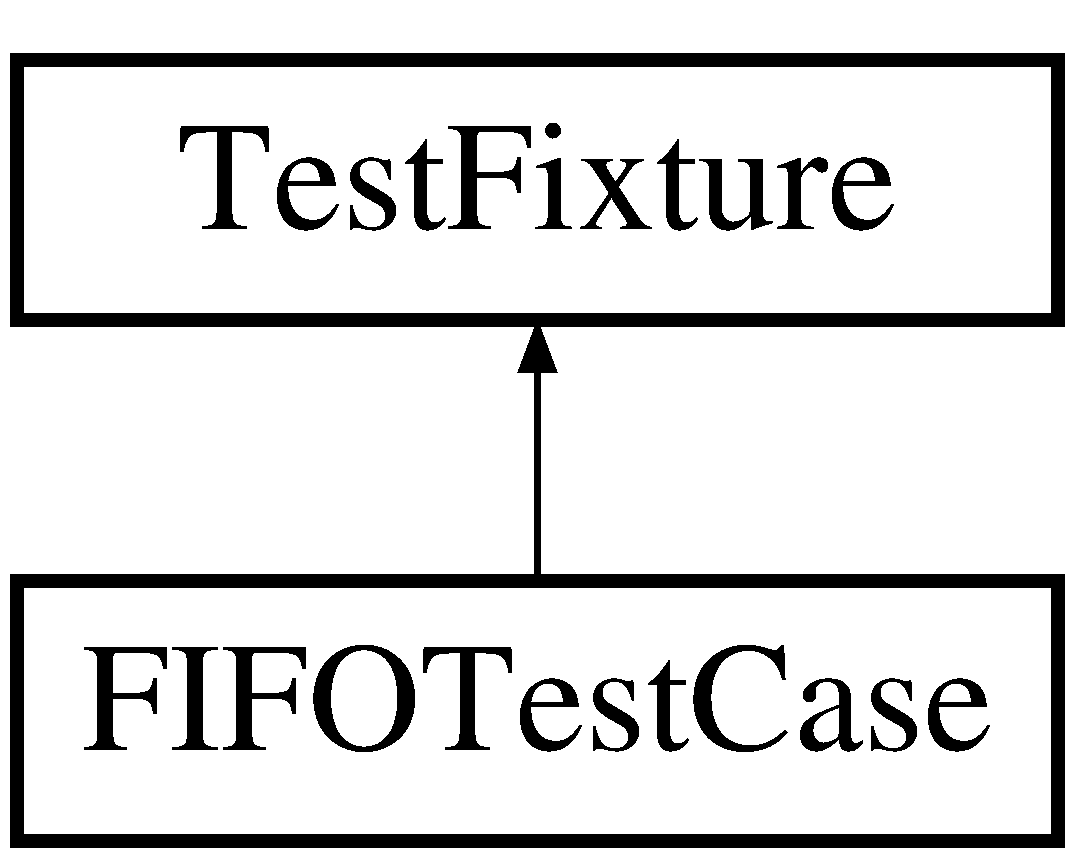
\includegraphics[height=2.000000cm]{class_f_i_f_o_test_case}
\end{center}
\end{figure}
\subsection*{Public Member Functions}
\begin{DoxyCompactItemize}
\item 
void \hyperlink{class_f_i_f_o_test_case_a495f68d6fc339a408d0fba28cc50ebc6}{set\+Up} ()
\item 
void \hyperlink{class_f_i_f_o_test_case_a584d644de7aa5dcb2027b3f4ea8da683}{tear\+Down} ()
\item 
void \hyperlink{class_f_i_f_o_test_case_adef49d5e56109bf1ed0f23210c57d761}{test\+\_\+pop\+\_\+task} ()
\item 
void \hyperlink{class_f_i_f_o_test_case_a749871e27042f119be009b27bc082136}{test\+\_\+push\+\_\+new\+\_\+task} ()
\item 
void \hyperlink{class_f_i_f_o_test_case_a53bda2037e4df5fd0be76a8485766b27}{test\+\_\+is\+\_\+statistic\+\_\+based} ()
\item 
void \hyperlink{class_f_i_f_o_test_case_a0e5bf8bbab4e77bce4092bc0b3c5192b}{test\+\_\+get\+\_\+count} ()
\item 
void \hyperlink{class_f_i_f_o_test_case_a8f870e880a9d9092042ac5f7d55a120a}{test\+\_\+get\+\_\+next\+\_\+task} ()
\end{DoxyCompactItemize}
\subsection*{Static Public Member Functions}
\begin{DoxyCompactItemize}
\item 
static Test $\ast$ \hyperlink{class_f_i_f_o_test_case_ad80f96dab4623dcaf147db1582af9574}{suite} ()
\end{DoxyCompactItemize}


\subsection{Detailed Description}


Definition at line 24 of file F\+I\+F\+O\+Test\+Case.\+h.



\subsection{Member Function Documentation}
\hypertarget{class_f_i_f_o_test_case_a495f68d6fc339a408d0fba28cc50ebc6}{}\index{F\+I\+F\+O\+Test\+Case@{F\+I\+F\+O\+Test\+Case}!set\+Up@{set\+Up}}
\index{set\+Up@{set\+Up}!F\+I\+F\+O\+Test\+Case@{F\+I\+F\+O\+Test\+Case}}
\subsubsection[{set\+Up}]{\setlength{\rightskip}{0pt plus 5cm}void F\+I\+F\+O\+Test\+Case\+::set\+Up (
\begin{DoxyParamCaption}
{}
\end{DoxyParamCaption}
)}\label{class_f_i_f_o_test_case_a495f68d6fc339a408d0fba28cc50ebc6}


Definition at line 30 of file F\+I\+F\+O\+Test\+Case.\+cpp.

\hypertarget{class_f_i_f_o_test_case_ad80f96dab4623dcaf147db1582af9574}{}\index{F\+I\+F\+O\+Test\+Case@{F\+I\+F\+O\+Test\+Case}!suite@{suite}}
\index{suite@{suite}!F\+I\+F\+O\+Test\+Case@{F\+I\+F\+O\+Test\+Case}}
\subsubsection[{suite}]{\setlength{\rightskip}{0pt plus 5cm}Test $\ast$ F\+I\+F\+O\+Test\+Case\+::suite (
\begin{DoxyParamCaption}
{}
\end{DoxyParamCaption}
)\hspace{0.3cm}{\ttfamily [static]}}\label{class_f_i_f_o_test_case_ad80f96dab4623dcaf147db1582af9574}


Definition at line 19 of file F\+I\+F\+O\+Test\+Case.\+cpp.

\hypertarget{class_f_i_f_o_test_case_a584d644de7aa5dcb2027b3f4ea8da683}{}\index{F\+I\+F\+O\+Test\+Case@{F\+I\+F\+O\+Test\+Case}!tear\+Down@{tear\+Down}}
\index{tear\+Down@{tear\+Down}!F\+I\+F\+O\+Test\+Case@{F\+I\+F\+O\+Test\+Case}}
\subsubsection[{tear\+Down}]{\setlength{\rightskip}{0pt plus 5cm}void F\+I\+F\+O\+Test\+Case\+::tear\+Down (
\begin{DoxyParamCaption}
{}
\end{DoxyParamCaption}
)}\label{class_f_i_f_o_test_case_a584d644de7aa5dcb2027b3f4ea8da683}


Definition at line 34 of file F\+I\+F\+O\+Test\+Case.\+cpp.

\hypertarget{class_f_i_f_o_test_case_a0e5bf8bbab4e77bce4092bc0b3c5192b}{}\index{F\+I\+F\+O\+Test\+Case@{F\+I\+F\+O\+Test\+Case}!test\+\_\+get\+\_\+count@{test\+\_\+get\+\_\+count}}
\index{test\+\_\+get\+\_\+count@{test\+\_\+get\+\_\+count}!F\+I\+F\+O\+Test\+Case@{F\+I\+F\+O\+Test\+Case}}
\subsubsection[{test\+\_\+get\+\_\+count}]{\setlength{\rightskip}{0pt plus 5cm}void F\+I\+F\+O\+Test\+Case\+::test\+\_\+get\+\_\+count (
\begin{DoxyParamCaption}
{}
\end{DoxyParamCaption}
)}\label{class_f_i_f_o_test_case_a0e5bf8bbab4e77bce4092bc0b3c5192b}


Definition at line 42 of file F\+I\+F\+O\+Test\+Case.\+cpp.

\hypertarget{class_f_i_f_o_test_case_a8f870e880a9d9092042ac5f7d55a120a}{}\index{F\+I\+F\+O\+Test\+Case@{F\+I\+F\+O\+Test\+Case}!test\+\_\+get\+\_\+next\+\_\+task@{test\+\_\+get\+\_\+next\+\_\+task}}
\index{test\+\_\+get\+\_\+next\+\_\+task@{test\+\_\+get\+\_\+next\+\_\+task}!F\+I\+F\+O\+Test\+Case@{F\+I\+F\+O\+Test\+Case}}
\subsubsection[{test\+\_\+get\+\_\+next\+\_\+task}]{\setlength{\rightskip}{0pt plus 5cm}void F\+I\+F\+O\+Test\+Case\+::test\+\_\+get\+\_\+next\+\_\+task (
\begin{DoxyParamCaption}
{}
\end{DoxyParamCaption}
)}\label{class_f_i_f_o_test_case_a8f870e880a9d9092042ac5f7d55a120a}


Definition at line 79 of file F\+I\+F\+O\+Test\+Case.\+cpp.

\hypertarget{class_f_i_f_o_test_case_a53bda2037e4df5fd0be76a8485766b27}{}\index{F\+I\+F\+O\+Test\+Case@{F\+I\+F\+O\+Test\+Case}!test\+\_\+is\+\_\+statistic\+\_\+based@{test\+\_\+is\+\_\+statistic\+\_\+based}}
\index{test\+\_\+is\+\_\+statistic\+\_\+based@{test\+\_\+is\+\_\+statistic\+\_\+based}!F\+I\+F\+O\+Test\+Case@{F\+I\+F\+O\+Test\+Case}}
\subsubsection[{test\+\_\+is\+\_\+statistic\+\_\+based}]{\setlength{\rightskip}{0pt plus 5cm}void F\+I\+F\+O\+Test\+Case\+::test\+\_\+is\+\_\+statistic\+\_\+based (
\begin{DoxyParamCaption}
{}
\end{DoxyParamCaption}
)}\label{class_f_i_f_o_test_case_a53bda2037e4df5fd0be76a8485766b27}


Definition at line 38 of file F\+I\+F\+O\+Test\+Case.\+cpp.

\hypertarget{class_f_i_f_o_test_case_adef49d5e56109bf1ed0f23210c57d761}{}\index{F\+I\+F\+O\+Test\+Case@{F\+I\+F\+O\+Test\+Case}!test\+\_\+pop\+\_\+task@{test\+\_\+pop\+\_\+task}}
\index{test\+\_\+pop\+\_\+task@{test\+\_\+pop\+\_\+task}!F\+I\+F\+O\+Test\+Case@{F\+I\+F\+O\+Test\+Case}}
\subsubsection[{test\+\_\+pop\+\_\+task}]{\setlength{\rightskip}{0pt plus 5cm}void F\+I\+F\+O\+Test\+Case\+::test\+\_\+pop\+\_\+task (
\begin{DoxyParamCaption}
{}
\end{DoxyParamCaption}
)}\label{class_f_i_f_o_test_case_adef49d5e56109bf1ed0f23210c57d761}


Definition at line 53 of file F\+I\+F\+O\+Test\+Case.\+cpp.

\hypertarget{class_f_i_f_o_test_case_a749871e27042f119be009b27bc082136}{}\index{F\+I\+F\+O\+Test\+Case@{F\+I\+F\+O\+Test\+Case}!test\+\_\+push\+\_\+new\+\_\+task@{test\+\_\+push\+\_\+new\+\_\+task}}
\index{test\+\_\+push\+\_\+new\+\_\+task@{test\+\_\+push\+\_\+new\+\_\+task}!F\+I\+F\+O\+Test\+Case@{F\+I\+F\+O\+Test\+Case}}
\subsubsection[{test\+\_\+push\+\_\+new\+\_\+task}]{\setlength{\rightskip}{0pt plus 5cm}void F\+I\+F\+O\+Test\+Case\+::test\+\_\+push\+\_\+new\+\_\+task (
\begin{DoxyParamCaption}
{}
\end{DoxyParamCaption}
)}\label{class_f_i_f_o_test_case_a749871e27042f119be009b27bc082136}


Definition at line 68 of file F\+I\+F\+O\+Test\+Case.\+cpp.



The documentation for this class was generated from the following files\+:\begin{DoxyCompactItemize}
\item 
test/scheduler/\hyperlink{_f_i_f_o_test_case_8h}{F\+I\+F\+O\+Test\+Case.\+h}\item 
test/scheduler/\hyperlink{_f_i_f_o_test_case_8cpp}{F\+I\+F\+O\+Test\+Case.\+cpp}\end{DoxyCompactItemize}

\hypertarget{classel_1_1base_1_1utils_1_1_file}{}\section{el\+:\+:base\+:\+:utils\+:\+:File Class Reference}
\label{classel_1_1base_1_1utils_1_1_file}\index{el\+::base\+::utils\+::\+File@{el\+::base\+::utils\+::\+File}}


{\ttfamily \#include $<$easylogging++.\+h$>$}

Inheritance diagram for el\+:\+:base\+:\+:utils\+:\+:File\+:\begin{figure}[H]
\begin{center}
\leavevmode
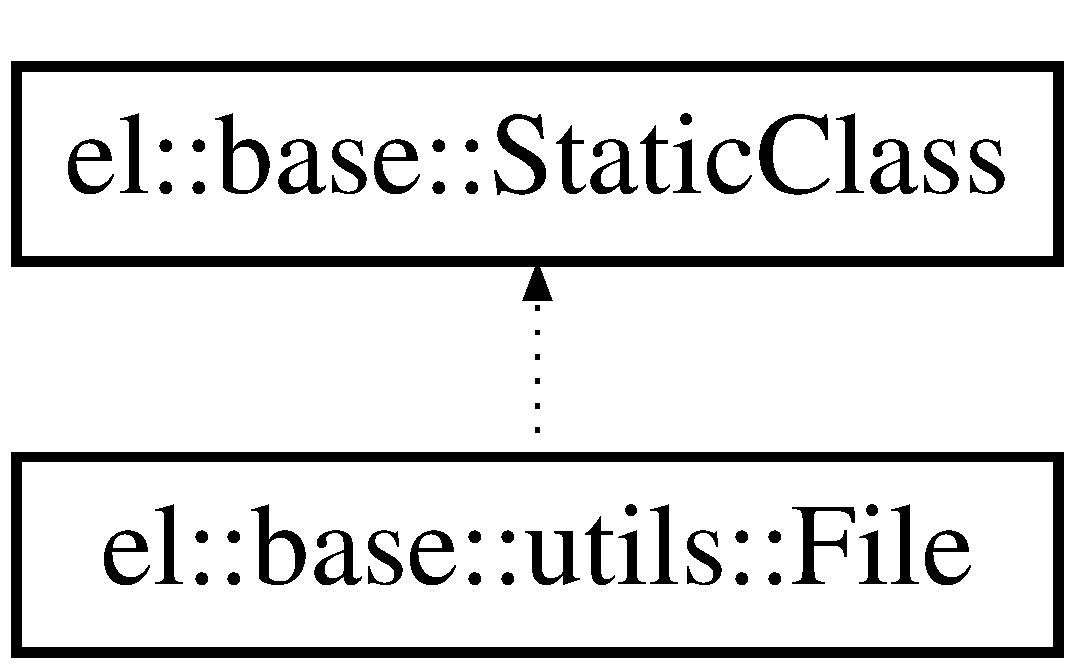
\includegraphics[height=2.000000cm]{classel_1_1base_1_1utils_1_1_file}
\end{center}
\end{figure}
\subsection*{Static Public Member Functions}
\begin{DoxyCompactItemize}
\item 
static \hyperlink{namespaceel_1_1base_1_1type_a620c830ead75d26b45c060c211ee2685}{base\+::type\+::fstream\+\_\+t} $\ast$ \hyperlink{classel_1_1base_1_1utils_1_1_file_aa4bef1f2e00269d75c1c1eabb0ce4563}{new\+File\+Stream} (const std\+::string \&filename)
\begin{DoxyCompactList}\small\item\em Creates new out file stream for specified filename. \end{DoxyCompactList}\item 
static std\+::size\+\_\+t \hyperlink{classel_1_1base_1_1utils_1_1_file_a54415ba02f698ba978795265f7f4b86c}{get\+Size\+Of\+File} (\hyperlink{namespaceel_1_1base_1_1type_a620c830ead75d26b45c060c211ee2685}{base\+::type\+::fstream\+\_\+t} $\ast$fs)
\begin{DoxyCompactList}\small\item\em Gets size of file provided in stream. \end{DoxyCompactList}\item 
static bool \hyperlink{classel_1_1base_1_1utils_1_1_file_a4fc9e36b814f1aeaa4931e35d58e5b45}{path\+Exists} (const char $\ast$path, bool consider\+File=false)
\begin{DoxyCompactList}\small\item\em Determines whether or not provided path exist in current file system. \end{DoxyCompactList}\item 
static bool \hyperlink{classel_1_1base_1_1utils_1_1_file_a34fbb5b06201c7e3db71db80e017fb96}{create\+Path} (const std\+::string \&path)
\begin{DoxyCompactList}\small\item\em Creates specified path on file system. \end{DoxyCompactList}\item 
static std\+::string \hyperlink{classel_1_1base_1_1utils_1_1_file_af541c62ed408de7e368d339f96c0c6cf}{extract\+Path\+From\+Filename} (const std\+::string \&full\+Path, const char $\ast$seperator=base\+::consts\+::k\+File\+Path\+Seperator)
\begin{DoxyCompactList}\small\item\em Extracts path of filename with leading slash. \end{DoxyCompactList}\item 
static void \hyperlink{classel_1_1base_1_1utils_1_1_file_a38e3b3c72f73de47563b289eff13ae2d}{build\+Stripped\+Filename} (const char $\ast$filename, char buff\mbox{[}$\,$\mbox{]}, std\+::size\+\_\+t limit=base\+::consts\+::k\+Source\+Filename\+Max\+Length)
\begin{DoxyCompactList}\small\item\em builds stripped filename and puts it in buff \end{DoxyCompactList}\item 
static void \hyperlink{classel_1_1base_1_1utils_1_1_file_ad6c3703c16b95bd4992f501380d503b4}{build\+Base\+Filename} (const std\+::string \&full\+Path, char buff\mbox{[}$\,$\mbox{]}, std\+::size\+\_\+t limit=base\+::consts\+::k\+Source\+Filename\+Max\+Length, const char $\ast$seperator=base\+::consts\+::k\+File\+Path\+Seperator)
\begin{DoxyCompactList}\small\item\em builds base filename and puts it in buff \end{DoxyCompactList}\end{DoxyCompactItemize}


\subsection{Detailed Description}


Definition at line 1083 of file easylogging++.\+h.



\subsection{Member Function Documentation}
\hypertarget{classel_1_1base_1_1utils_1_1_file_ad6c3703c16b95bd4992f501380d503b4}{}\index{el\+::base\+::utils\+::\+File@{el\+::base\+::utils\+::\+File}!build\+Base\+Filename@{build\+Base\+Filename}}
\index{build\+Base\+Filename@{build\+Base\+Filename}!el\+::base\+::utils\+::\+File@{el\+::base\+::utils\+::\+File}}
\subsubsection[{build\+Base\+Filename}]{\setlength{\rightskip}{0pt plus 5cm}static void el\+::base\+::utils\+::\+File\+::build\+Base\+Filename (
\begin{DoxyParamCaption}
\item[{const std\+::string \&}]{full\+Path, }
\item[{char}]{buff\mbox{[}$\,$\mbox{]}, }
\item[{std\+::size\+\_\+t}]{limit = {\ttfamily base\+:\+:consts\+:\+:kSourceFilenameMaxLength}, }
\item[{const char $\ast$}]{seperator = {\ttfamily base\+:\+:consts\+:\+:kFilePathSeperator}}
\end{DoxyParamCaption}
)\hspace{0.3cm}{\ttfamily [inline]}, {\ttfamily [static]}}\label{classel_1_1base_1_1utils_1_1_file_ad6c3703c16b95bd4992f501380d503b4}


builds base filename and puts it in buff 



Definition at line 1204 of file easylogging++.\+h.

\hypertarget{classel_1_1base_1_1utils_1_1_file_a38e3b3c72f73de47563b289eff13ae2d}{}\index{el\+::base\+::utils\+::\+File@{el\+::base\+::utils\+::\+File}!build\+Stripped\+Filename@{build\+Stripped\+Filename}}
\index{build\+Stripped\+Filename@{build\+Stripped\+Filename}!el\+::base\+::utils\+::\+File@{el\+::base\+::utils\+::\+File}}
\subsubsection[{build\+Stripped\+Filename}]{\setlength{\rightskip}{0pt plus 5cm}static void el\+::base\+::utils\+::\+File\+::build\+Stripped\+Filename (
\begin{DoxyParamCaption}
\item[{const char $\ast$}]{filename, }
\item[{char}]{buff\mbox{[}$\,$\mbox{]}, }
\item[{std\+::size\+\_\+t}]{limit = {\ttfamily base\+:\+:consts\+:\+:kSourceFilenameMaxLength}}
\end{DoxyParamCaption}
)\hspace{0.3cm}{\ttfamily [inline]}, {\ttfamily [static]}}\label{classel_1_1base_1_1utils_1_1_file_a38e3b3c72f73de47563b289eff13ae2d}


builds stripped filename and puts it in buff 



Definition at line 1191 of file easylogging++.\+h.

\hypertarget{classel_1_1base_1_1utils_1_1_file_a34fbb5b06201c7e3db71db80e017fb96}{}\index{el\+::base\+::utils\+::\+File@{el\+::base\+::utils\+::\+File}!create\+Path@{create\+Path}}
\index{create\+Path@{create\+Path}!el\+::base\+::utils\+::\+File@{el\+::base\+::utils\+::\+File}}
\subsubsection[{create\+Path}]{\setlength{\rightskip}{0pt plus 5cm}static bool el\+::base\+::utils\+::\+File\+::create\+Path (
\begin{DoxyParamCaption}
\item[{const std\+::string \&}]{path}
\end{DoxyParamCaption}
)\hspace{0.3cm}{\ttfamily [inline]}, {\ttfamily [static]}}\label{classel_1_1base_1_1utils_1_1_file_a34fbb5b06201c7e3db71db80e017fb96}


Creates specified path on file system. 


\begin{DoxyParams}{Parameters}
{\em path} & Path to create. \\
\hline
\end{DoxyParams}


Definition at line 1139 of file easylogging++.\+h.

\hypertarget{classel_1_1base_1_1utils_1_1_file_af541c62ed408de7e368d339f96c0c6cf}{}\index{el\+::base\+::utils\+::\+File@{el\+::base\+::utils\+::\+File}!extract\+Path\+From\+Filename@{extract\+Path\+From\+Filename}}
\index{extract\+Path\+From\+Filename@{extract\+Path\+From\+Filename}!el\+::base\+::utils\+::\+File@{el\+::base\+::utils\+::\+File}}
\subsubsection[{extract\+Path\+From\+Filename}]{\setlength{\rightskip}{0pt plus 5cm}static std\+::string el\+::base\+::utils\+::\+File\+::extract\+Path\+From\+Filename (
\begin{DoxyParamCaption}
\item[{const std\+::string \&}]{full\+Path, }
\item[{const char $\ast$}]{seperator = {\ttfamily base\+:\+:consts\+:\+:kFilePathSeperator}}
\end{DoxyParamCaption}
)\hspace{0.3cm}{\ttfamily [inline]}, {\ttfamily [static]}}\label{classel_1_1base_1_1utils_1_1_file_af541c62ed408de7e368d339f96c0c6cf}


Extracts path of filename with leading slash. 



Definition at line 1179 of file easylogging++.\+h.

\hypertarget{classel_1_1base_1_1utils_1_1_file_a54415ba02f698ba978795265f7f4b86c}{}\index{el\+::base\+::utils\+::\+File@{el\+::base\+::utils\+::\+File}!get\+Size\+Of\+File@{get\+Size\+Of\+File}}
\index{get\+Size\+Of\+File@{get\+Size\+Of\+File}!el\+::base\+::utils\+::\+File@{el\+::base\+::utils\+::\+File}}
\subsubsection[{get\+Size\+Of\+File}]{\setlength{\rightskip}{0pt plus 5cm}static std\+::size\+\_\+t el\+::base\+::utils\+::\+File\+::get\+Size\+Of\+File (
\begin{DoxyParamCaption}
\item[{{\bf base\+::type\+::fstream\+\_\+t} $\ast$}]{fs}
\end{DoxyParamCaption}
)\hspace{0.3cm}{\ttfamily [inline]}, {\ttfamily [static]}}\label{classel_1_1base_1_1utils_1_1_file_a54415ba02f698ba978795265f7f4b86c}


Gets size of file provided in stream. 



Definition at line 1108 of file easylogging++.\+h.

\hypertarget{classel_1_1base_1_1utils_1_1_file_aa4bef1f2e00269d75c1c1eabb0ce4563}{}\index{el\+::base\+::utils\+::\+File@{el\+::base\+::utils\+::\+File}!new\+File\+Stream@{new\+File\+Stream}}
\index{new\+File\+Stream@{new\+File\+Stream}!el\+::base\+::utils\+::\+File@{el\+::base\+::utils\+::\+File}}
\subsubsection[{new\+File\+Stream}]{\setlength{\rightskip}{0pt plus 5cm}static {\bf base\+::type\+::fstream\+\_\+t}$\ast$ el\+::base\+::utils\+::\+File\+::new\+File\+Stream (
\begin{DoxyParamCaption}
\item[{const std\+::string \&}]{filename}
\end{DoxyParamCaption}
)\hspace{0.3cm}{\ttfamily [inline]}, {\ttfamily [static]}}\label{classel_1_1base_1_1utils_1_1_file_aa4bef1f2e00269d75c1c1eabb0ce4563}


Creates new out file stream for specified filename. 

\begin{DoxyReturn}{Returns}
Pointer to newly created fstream or nullptr 
\end{DoxyReturn}


Definition at line 1087 of file easylogging++.\+h.

\hypertarget{classel_1_1base_1_1utils_1_1_file_a4fc9e36b814f1aeaa4931e35d58e5b45}{}\index{el\+::base\+::utils\+::\+File@{el\+::base\+::utils\+::\+File}!path\+Exists@{path\+Exists}}
\index{path\+Exists@{path\+Exists}!el\+::base\+::utils\+::\+File@{el\+::base\+::utils\+::\+File}}
\subsubsection[{path\+Exists}]{\setlength{\rightskip}{0pt plus 5cm}static bool el\+::base\+::utils\+::\+File\+::path\+Exists (
\begin{DoxyParamCaption}
\item[{const char $\ast$}]{path, }
\item[{bool}]{consider\+File = {\ttfamily false}}
\end{DoxyParamCaption}
)\hspace{0.3cm}{\ttfamily [inline]}, {\ttfamily [static]}}\label{classel_1_1base_1_1utils_1_1_file_a4fc9e36b814f1aeaa4931e35d58e5b45}


Determines whether or not provided path exist in current file system. 



Definition at line 1120 of file easylogging++.\+h.



The documentation for this class was generated from the following file\+:\begin{DoxyCompactItemize}
\item 
lib/\hyperlink{easylogging_09_09_8h}{easylogging++.\+h}\end{DoxyCompactItemize}

\hypertarget{class_grid_creator}{}\section{Grid\+Creator Class Reference}
\label{class_grid_creator}\index{Grid\+Creator@{Grid\+Creator}}


{\ttfamily \#include $<$Grid\+Creator.\+h$>$}

\subsection*{Public Member Functions}
\begin{DoxyCompactItemize}
\item 
long \hyperlink{class_grid_creator_a2a1ef6eaef2cabb482c19ef55d168249}{predict} (double $\ast$parameters, int parameter\+\_\+count)
\end{DoxyCompactItemize}


\subsection{Detailed Description}
Project Dynamic Scheduler for Scientific Simulations 

Definition at line 10 of file Grid\+Creator.\+h.



\subsection{Member Function Documentation}
\hypertarget{class_grid_creator_a2a1ef6eaef2cabb482c19ef55d168249}{}\index{Grid\+Creator@{Grid\+Creator}!predict@{predict}}
\index{predict@{predict}!Grid\+Creator@{Grid\+Creator}}
\subsubsection[{predict}]{\setlength{\rightskip}{0pt plus 5cm}long Grid\+Creator\+::predict (
\begin{DoxyParamCaption}
\item[{double $\ast$}]{parameters, }
\item[{int}]{parameter\+\_\+count}
\end{DoxyParamCaption}
)}\label{class_grid_creator_a2a1ef6eaef2cabb482c19ef55d168249}


The documentation for this class was generated from the following file\+:\begin{DoxyCompactItemize}
\item 
src/datamining/grid/\hyperlink{_grid_creator_8h}{Grid\+Creator.\+h}\end{DoxyCompactItemize}

\hypertarget{class_grid_data_mining}{}\section{Grid\+Data\+Mining Class Reference}
\label{class_grid_data_mining}\index{Grid\+Data\+Mining@{Grid\+Data\+Mining}}


{\ttfamily \#include $<$Grid\+Data\+Mining.\+h$>$}

Inheritance diagram for Grid\+Data\+Mining\+:\begin{figure}[H]
\begin{center}
\leavevmode
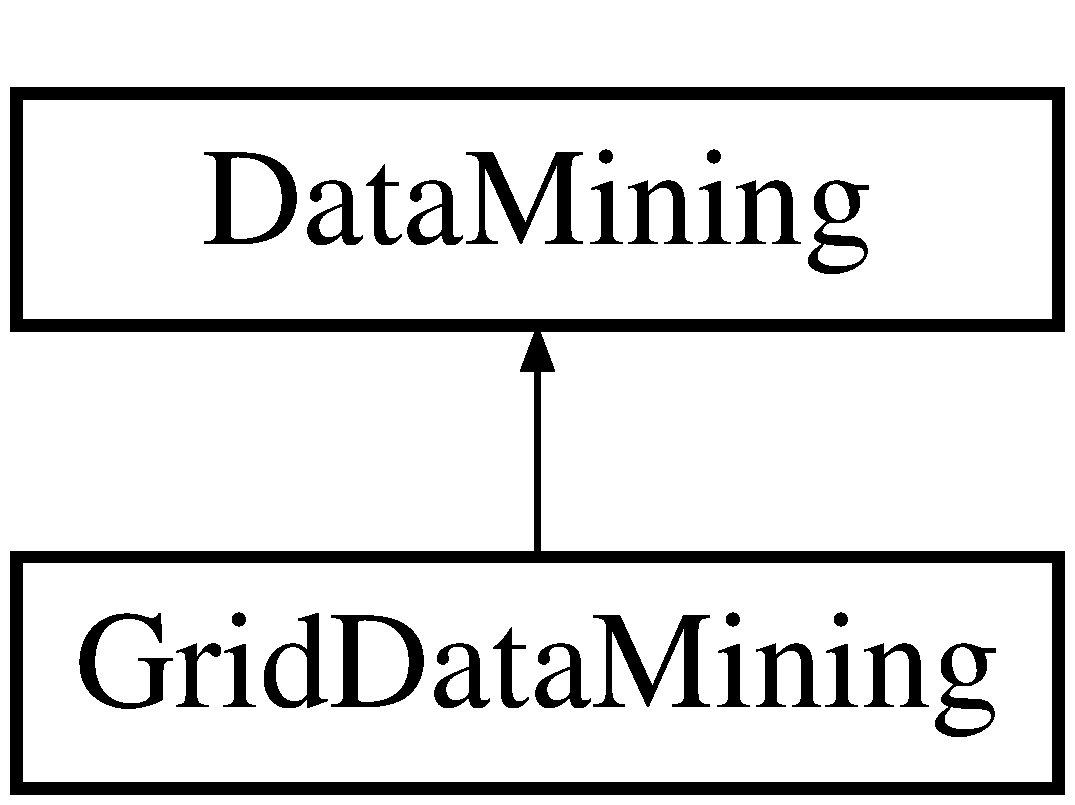
\includegraphics[height=2.000000cm]{class_grid_data_mining}
\end{center}
\end{figure}
\subsection*{Public Member Functions}
\begin{DoxyCompactItemize}
\item 
\hyperlink{class_grid_data_mining_a102921a759bec8661c748256391d8ae8}{Grid\+Data\+Mining} (int parameter\+\_\+count, long default\+\_\+value)
\item 
long \hyperlink{class_grid_data_mining_a8aef1fbc6d1f034660efee2878f2efe2}{predict} (double $\ast$parameters)
\item 
void \hyperlink{class_grid_data_mining_a864374110fb8c1673c057f524776ff97}{insert} (double $\ast$parameters, long runtime)
\end{DoxyCompactItemize}


\subsection{Detailed Description}
Project Dynamic Scheduler for Scientific Simulations 

Definition at line 11 of file Grid\+Data\+Mining.\+h.



\subsection{Constructor \& Destructor Documentation}
\hypertarget{class_grid_data_mining_a102921a759bec8661c748256391d8ae8}{}\index{Grid\+Data\+Mining@{Grid\+Data\+Mining}!Grid\+Data\+Mining@{Grid\+Data\+Mining}}
\index{Grid\+Data\+Mining@{Grid\+Data\+Mining}!Grid\+Data\+Mining@{Grid\+Data\+Mining}}
\subsubsection[{Grid\+Data\+Mining}]{\setlength{\rightskip}{0pt plus 5cm}Grid\+Data\+Mining\+::\+Grid\+Data\+Mining (
\begin{DoxyParamCaption}
\item[{int}]{parameter\+\_\+count, }
\item[{long}]{default\+\_\+value}
\end{DoxyParamCaption}
)}\label{class_grid_data_mining_a102921a759bec8661c748256391d8ae8}
Grid\+Data\+Minig implementation 

Definition at line 7 of file Grid\+Data\+Mining.\+cpp.



\subsection{Member Function Documentation}
\hypertarget{class_grid_data_mining_a864374110fb8c1673c057f524776ff97}{}\index{Grid\+Data\+Mining@{Grid\+Data\+Mining}!insert@{insert}}
\index{insert@{insert}!Grid\+Data\+Mining@{Grid\+Data\+Mining}}
\subsubsection[{insert}]{\setlength{\rightskip}{0pt plus 5cm}void Grid\+Data\+Mining\+::insert (
\begin{DoxyParamCaption}
\item[{double $\ast$}]{parameters, }
\item[{long}]{runtime}
\end{DoxyParamCaption}
)\hspace{0.3cm}{\ttfamily [virtual]}}\label{class_grid_data_mining_a864374110fb8c1673c057f524776ff97}


Implements \hyperlink{class_data_mining_ae4a8f82a2356d0b45d0e3c750a67aa5c}{Data\+Mining}.



Definition at line 18 of file Grid\+Data\+Mining.\+cpp.

\hypertarget{class_grid_data_mining_a8aef1fbc6d1f034660efee2878f2efe2}{}\index{Grid\+Data\+Mining@{Grid\+Data\+Mining}!predict@{predict}}
\index{predict@{predict}!Grid\+Data\+Mining@{Grid\+Data\+Mining}}
\subsubsection[{predict}]{\setlength{\rightskip}{0pt plus 5cm}long Grid\+Data\+Mining\+::predict (
\begin{DoxyParamCaption}
\item[{double $\ast$}]{parameters}
\end{DoxyParamCaption}
)\hspace{0.3cm}{\ttfamily [virtual]}}\label{class_grid_data_mining_a8aef1fbc6d1f034660efee2878f2efe2}


Implements \hyperlink{class_data_mining_a03b115a9db40dde60012bde4e4491966}{Data\+Mining}.



Definition at line 13 of file Grid\+Data\+Mining.\+cpp.



The documentation for this class was generated from the following files\+:\begin{DoxyCompactItemize}
\item 
src/datamining/grid/\hyperlink{_grid_data_mining_8h}{Grid\+Data\+Mining.\+h}\item 
src/datamining/grid/\hyperlink{_grid_data_mining_8cpp}{Grid\+Data\+Mining.\+cpp}\end{DoxyCompactItemize}

\hypertarget{class_grid_predictor}{}\section{Grid\+Predictor Class Reference}
\label{class_grid_predictor}\index{Grid\+Predictor@{Grid\+Predictor}}


{\ttfamily \#include $<$Grid\+Predictor.\+h$>$}

\subsection*{Public Member Functions}
\begin{DoxyCompactItemize}
\item 
long \hyperlink{class_grid_predictor_a357524a8315c708b29ec1b344c356995}{predict} (double $\ast$parameters, int parameter\+\_\+count)
\end{DoxyCompactItemize}


\subsection{Detailed Description}
Project Dynamic Scheduler for Scientific Simulations 

Definition at line 10 of file Grid\+Predictor.\+h.



\subsection{Member Function Documentation}
\hypertarget{class_grid_predictor_a357524a8315c708b29ec1b344c356995}{}\index{Grid\+Predictor@{Grid\+Predictor}!predict@{predict}}
\index{predict@{predict}!Grid\+Predictor@{Grid\+Predictor}}
\subsubsection[{predict}]{\setlength{\rightskip}{0pt plus 5cm}long Grid\+Predictor\+::predict (
\begin{DoxyParamCaption}
\item[{double $\ast$}]{parameters, }
\item[{int}]{parameter\+\_\+count}
\end{DoxyParamCaption}
)}\label{class_grid_predictor_a357524a8315c708b29ec1b344c356995}


Definition at line 3 of file Gird\+Predictor.\+cpp.



The documentation for this class was generated from the following files\+:\begin{DoxyCompactItemize}
\item 
src/datamining/grid/\hyperlink{_grid_predictor_8h}{Grid\+Predictor.\+h}\item 
src/datamining/grid/\hyperlink{_gird_predictor_8cpp}{Gird\+Predictor.\+cpp}\end{DoxyCompactItemize}

\hypertarget{classel_1_1_helpers}{}\section{el\+:\+:Helpers Class Reference}
\label{classel_1_1_helpers}\index{el\+::\+Helpers@{el\+::\+Helpers}}


Static helpers for developers.  




{\ttfamily \#include $<$easylogging++.\+h$>$}

Inheritance diagram for el\+:\+:Helpers\+:\begin{figure}[H]
\begin{center}
\leavevmode
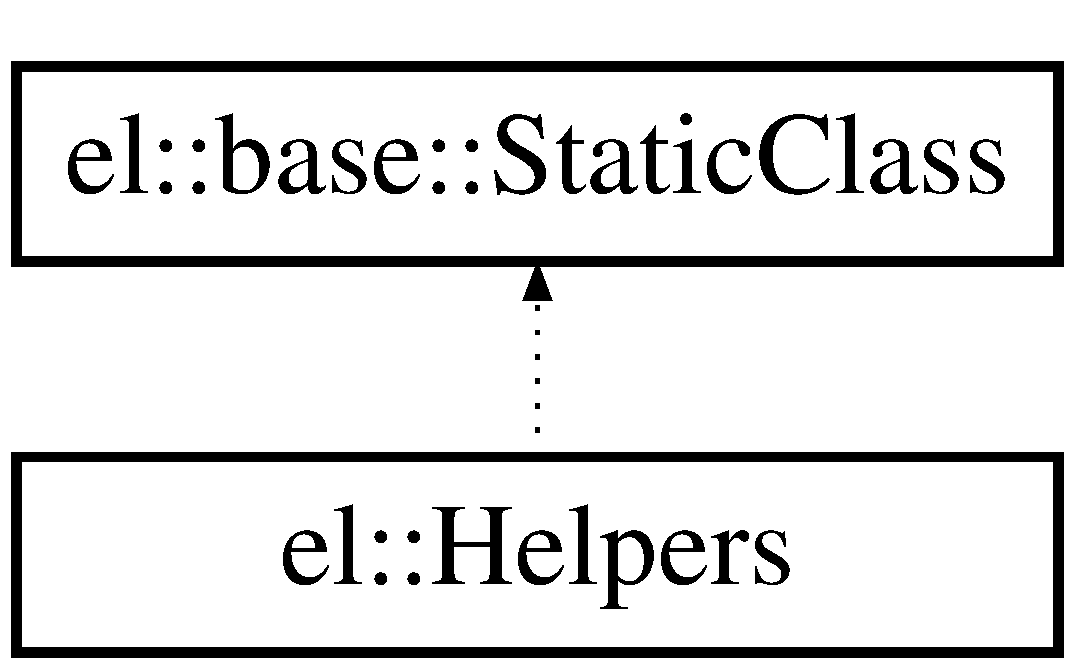
\includegraphics[height=2.000000cm]{classel_1_1_helpers}
\end{center}
\end{figure}
\subsection*{Static Public Member Functions}
\begin{DoxyCompactItemize}
\item 
static void \hyperlink{classel_1_1_helpers_af78fd39725281e3dddd7c0fbdc14f11f}{set\+Storage} (\hyperlink{namespaceel_1_1base_1_1type_a3c34822c3825018aca1526f2289b7976}{base\+::type\+::\+Storage\+Pointer} \hyperlink{classel_1_1_helpers_a13a5365de36b3af27660cf9b358829d3}{storage})
\begin{DoxyCompactList}\small\item\em Shares logging repository (\hyperlink{classel_1_1base_1_1_storage}{base\+::\+Storage}) \end{DoxyCompactList}\item 
static \hyperlink{namespaceel_1_1base_1_1type_a3c34822c3825018aca1526f2289b7976}{base\+::type\+::\+Storage\+Pointer} \hyperlink{classel_1_1_helpers_a13a5365de36b3af27660cf9b358829d3}{storage} ()
\item 
static void \hyperlink{classel_1_1_helpers_a68748f618a0c2840b96dc12532b09bf0}{set\+Args} (int argc, char $\ast$$\ast$argv)
\begin{DoxyCompactList}\small\item\em Sets application arguments and figures out whats active for logging and whats not. \end{DoxyCompactList}\item 
static void \hyperlink{classel_1_1_helpers_afac7a023e2c13a62d0295cf0239eb848}{set\+Args} (int argc, const char $\ast$$\ast$argv)
\begin{DoxyCompactList}\small\item\em Sets application arguments and figures out whats active for logging and whats not. \end{DoxyCompactList}\item 
static void \hyperlink{classel_1_1_helpers_a4155f6fff0074ad93aa56fd7fe064097}{set\+Crash\+Handler} (const \hyperlink{classel_1_1base_1_1debug_1_1_crash_handler_aebf80d2fd5180d9c56db5a7e9abc7ad9}{el\+::base\+::debug\+::\+Crash\+Handler\+::\+Handler} \&crash\+Handler)
\begin{DoxyCompactList}\small\item\em Overrides default crash handler and installs custom handler. \end{DoxyCompactList}\item 
static void \hyperlink{classel_1_1_helpers_a6e16f0e07ce40e0659fcfec4ea5b6fe1}{crash\+Abort} (int sig, const char $\ast$source\+File=\char`\"{}\char`\"{}, unsigned int long line=0)
\begin{DoxyCompactList}\small\item\em Abort due to crash with signal in parameter. \end{DoxyCompactList}\item 
static void \hyperlink{classel_1_1_helpers_abf1ae61428740e1e6c5d5f0c36500faa}{log\+Crash\+Reason} (int sig, bool stack\+Trace\+If\+Available=false, \hyperlink{namespaceel_ab0ac6091262344c52dd2d3ad099e8e36}{Level} level=\hyperlink{namespaceel_ab0ac6091262344c52dd2d3ad099e8e36a882384ec38ce8d9582b57e70861730e4}{Level\+::\+Fatal}, const char $\ast$logger=base\+::consts\+::k\+Default\+Logger\+Id)
\begin{DoxyCompactList}\small\item\em Logs reason of crash as per sig. \end{DoxyCompactList}\item 
static void \hyperlink{classel_1_1_helpers_a5fd7ad6d636c28d2e706203d0c43cf8c}{install\+Pre\+Roll\+Out\+Callback} (const \hyperlink{namespaceel_aeb764b890a6f3cd41d2726bcd4e9c0cf}{Pre\+Roll\+Out\+Callback} \&callback)
\begin{DoxyCompactList}\small\item\em Installs pre rollout callback, this callback is triggered when log file is about to be rolled out (can be useful for backing up) \end{DoxyCompactList}\item 
static void \hyperlink{classel_1_1_helpers_ab829e5ed1b43bf965f5c288bc0280376}{uninstall\+Pre\+Roll\+Out\+Callback} (void)
\begin{DoxyCompactList}\small\item\em Uninstalls pre rollout callback. \end{DoxyCompactList}\item 
{\footnotesize template$<$typename T $>$ }\\static bool \hyperlink{classel_1_1_helpers_a3f3e84057567a8ac568a35899318544a}{install\+Log\+Dispatch\+Callback} (const std\+::string \&id)
\begin{DoxyCompactList}\small\item\em Installs post log dispatch callback, this callback is triggered when log is dispatched. \end{DoxyCompactList}\item 
{\footnotesize template$<$typename T $>$ }\\static void \hyperlink{classel_1_1_helpers_ac94b44cc8d399a5842703126478300d7}{uninstall\+Log\+Dispatch\+Callback} (const std\+::string \&id)
\begin{DoxyCompactList}\small\item\em Uninstalls log dispatch callback. \end{DoxyCompactList}\item 
{\footnotesize template$<$typename T $>$ }\\static T $\ast$ \hyperlink{classel_1_1_helpers_aa01d59ca141bc75c4fdd78a34234611b}{log\+Dispatch\+Callback} (const std\+::string \&id)
\item 
{\footnotesize template$<$typename T $>$ }\\static bool \hyperlink{classel_1_1_helpers_a93e2727d3a7a5c06ccc41a2ae7fe1835}{install\+Performance\+Tracking\+Callback} (const std\+::string \&id)
\begin{DoxyCompactList}\small\item\em Installs post performance tracking callback, this callback is triggered when performance tracking is finished. \end{DoxyCompactList}\item 
{\footnotesize template$<$typename T $>$ }\\static void \hyperlink{classel_1_1_helpers_af1c5a4951991179dca4879ba05fb67a6}{uninstall\+Performance\+Tracking\+Callback} (const std\+::string \&id)
\begin{DoxyCompactList}\small\item\em Uninstalls post performance tracking handler. \end{DoxyCompactList}\item 
{\footnotesize template$<$typename T $>$ }\\static T $\ast$ \hyperlink{classel_1_1_helpers_a007844d35095b26301c9218b29d74049}{performance\+Tracking\+Callback} (const std\+::string \&id)
\item 
{\footnotesize template$<$typename T $>$ }\\static std\+::string \hyperlink{classel_1_1_helpers_a8b032e32cd042ddc4fef4e814bad1082}{convert\+Template\+To\+Std\+String} (const T \&templ)
\begin{DoxyCompactList}\small\item\em Converts template to std\+::string -\/ useful for loggable classes to log containers within log(std\+::ostream\&) const. \end{DoxyCompactList}\item 
static const \hyperlink{classel_1_1base_1_1utils_1_1_command_line_args}{el\+::base\+::utils\+::\+Command\+Line\+Args} $\ast$ \hyperlink{classel_1_1_helpers_a83bab44f77a4961f8f5231e7ce9917bb}{command\+Line\+Args} (void)
\begin{DoxyCompactList}\small\item\em Returns command line arguments (pointer) provided to easylogging++. \end{DoxyCompactList}\item 
static void \hyperlink{classel_1_1_helpers_aa6de15a09db4f2a6763a6652c0ea12b1}{install\+Custom\+Format\+Specifier} (const \hyperlink{classel_1_1_custom_format_specifier}{Custom\+Format\+Specifier} \&custom\+Format\+Specifier)
\begin{DoxyCompactList}\small\item\em Installs user defined format specifier and handler. \end{DoxyCompactList}\item 
static bool \hyperlink{classel_1_1_helpers_a23ec73819c25758d604d149ad0c6b73f}{uninstall\+Custom\+Format\+Specifier} (const char $\ast$format\+Specifier)
\begin{DoxyCompactList}\small\item\em Uninstalls user defined format specifier and handler. \end{DoxyCompactList}\item 
static bool \hyperlink{classel_1_1_helpers_a154ce041890564d1ae5f87184e24f13d}{has\+Custom\+Format\+Specifier} (const char $\ast$format\+Specifier)
\begin{DoxyCompactList}\small\item\em Returns true if custom format specifier is installed. \end{DoxyCompactList}\item 
static void \hyperlink{classel_1_1_helpers_aea3fcde8a07e6f7278574e9563d8ab6b}{validate\+File\+Rolling} (\hyperlink{classel_1_1_logger}{Logger} $\ast$logger, \hyperlink{namespaceel_ab0ac6091262344c52dd2d3ad099e8e36}{Level} level)
\end{DoxyCompactItemize}


\subsection{Detailed Description}
Static helpers for developers. 

Definition at line 5648 of file easylogging++.\+h.



\subsection{Member Function Documentation}
\hypertarget{classel_1_1_helpers_a83bab44f77a4961f8f5231e7ce9917bb}{}\index{el\+::\+Helpers@{el\+::\+Helpers}!command\+Line\+Args@{command\+Line\+Args}}
\index{command\+Line\+Args@{command\+Line\+Args}!el\+::\+Helpers@{el\+::\+Helpers}}
\subsubsection[{command\+Line\+Args}]{\setlength{\rightskip}{0pt plus 5cm}static const {\bf el\+::base\+::utils\+::\+Command\+Line\+Args}$\ast$ el\+::\+Helpers\+::command\+Line\+Args (
\begin{DoxyParamCaption}
\item[{void}]{}
\end{DoxyParamCaption}
)\hspace{0.3cm}{\ttfamily [inline]}, {\ttfamily [static]}}\label{classel_1_1_helpers_a83bab44f77a4961f8f5231e7ce9917bb}


Returns command line arguments (pointer) provided to easylogging++. 



Definition at line 5755 of file easylogging++.\+h.

\hypertarget{classel_1_1_helpers_a8b032e32cd042ddc4fef4e814bad1082}{}\index{el\+::\+Helpers@{el\+::\+Helpers}!convert\+Template\+To\+Std\+String@{convert\+Template\+To\+Std\+String}}
\index{convert\+Template\+To\+Std\+String@{convert\+Template\+To\+Std\+String}!el\+::\+Helpers@{el\+::\+Helpers}}
\subsubsection[{convert\+Template\+To\+Std\+String}]{\setlength{\rightskip}{0pt plus 5cm}template$<$typename T $>$ static std\+::string el\+::\+Helpers\+::convert\+Template\+To\+Std\+String (
\begin{DoxyParamCaption}
\item[{const T \&}]{templ}
\end{DoxyParamCaption}
)\hspace{0.3cm}{\ttfamily [inline]}, {\ttfamily [static]}}\label{classel_1_1_helpers_a8b032e32cd042ddc4fef4e814bad1082}


Converts template to std\+::string -\/ useful for loggable classes to log containers within log(std\+::ostream\&) const. 



Definition at line 5735 of file easylogging++.\+h.

\hypertarget{classel_1_1_helpers_a6e16f0e07ce40e0659fcfec4ea5b6fe1}{}\index{el\+::\+Helpers@{el\+::\+Helpers}!crash\+Abort@{crash\+Abort}}
\index{crash\+Abort@{crash\+Abort}!el\+::\+Helpers@{el\+::\+Helpers}}
\subsubsection[{crash\+Abort}]{\setlength{\rightskip}{0pt plus 5cm}static void el\+::\+Helpers\+::crash\+Abort (
\begin{DoxyParamCaption}
\item[{int}]{sig, }
\item[{const char $\ast$}]{source\+File = {\ttfamily \char`\"{}\char`\"{}}, }
\item[{unsigned int long}]{line = {\ttfamily 0}}
\end{DoxyParamCaption}
)\hspace{0.3cm}{\ttfamily [inline]}, {\ttfamily [static]}}\label{classel_1_1_helpers_a6e16f0e07ce40e0659fcfec4ea5b6fe1}


Abort due to crash with signal in parameter. 


\begin{DoxyParams}{Parameters}
{\em sig} & Crash signal \\
\hline
\end{DoxyParams}


Definition at line 5674 of file easylogging++.\+h.

\hypertarget{classel_1_1_helpers_a154ce041890564d1ae5f87184e24f13d}{}\index{el\+::\+Helpers@{el\+::\+Helpers}!has\+Custom\+Format\+Specifier@{has\+Custom\+Format\+Specifier}}
\index{has\+Custom\+Format\+Specifier@{has\+Custom\+Format\+Specifier}!el\+::\+Helpers@{el\+::\+Helpers}}
\subsubsection[{has\+Custom\+Format\+Specifier}]{\setlength{\rightskip}{0pt plus 5cm}static bool el\+::\+Helpers\+::has\+Custom\+Format\+Specifier (
\begin{DoxyParamCaption}
\item[{const char $\ast$}]{format\+Specifier}
\end{DoxyParamCaption}
)\hspace{0.3cm}{\ttfamily [inline]}, {\ttfamily [static]}}\label{classel_1_1_helpers_a154ce041890564d1ae5f87184e24f13d}


Returns true if custom format specifier is installed. 



Definition at line 5767 of file easylogging++.\+h.

\hypertarget{classel_1_1_helpers_aa6de15a09db4f2a6763a6652c0ea12b1}{}\index{el\+::\+Helpers@{el\+::\+Helpers}!install\+Custom\+Format\+Specifier@{install\+Custom\+Format\+Specifier}}
\index{install\+Custom\+Format\+Specifier@{install\+Custom\+Format\+Specifier}!el\+::\+Helpers@{el\+::\+Helpers}}
\subsubsection[{install\+Custom\+Format\+Specifier}]{\setlength{\rightskip}{0pt plus 5cm}static void el\+::\+Helpers\+::install\+Custom\+Format\+Specifier (
\begin{DoxyParamCaption}
\item[{const {\bf Custom\+Format\+Specifier} \&}]{custom\+Format\+Specifier}
\end{DoxyParamCaption}
)\hspace{0.3cm}{\ttfamily [inline]}, {\ttfamily [static]}}\label{classel_1_1_helpers_aa6de15a09db4f2a6763a6652c0ea12b1}


Installs user defined format specifier and handler. 



Definition at line 5759 of file easylogging++.\+h.

\hypertarget{classel_1_1_helpers_a3f3e84057567a8ac568a35899318544a}{}\index{el\+::\+Helpers@{el\+::\+Helpers}!install\+Log\+Dispatch\+Callback@{install\+Log\+Dispatch\+Callback}}
\index{install\+Log\+Dispatch\+Callback@{install\+Log\+Dispatch\+Callback}!el\+::\+Helpers@{el\+::\+Helpers}}
\subsubsection[{install\+Log\+Dispatch\+Callback}]{\setlength{\rightskip}{0pt plus 5cm}template$<$typename T $>$ static bool el\+::\+Helpers\+::install\+Log\+Dispatch\+Callback (
\begin{DoxyParamCaption}
\item[{const std\+::string \&}]{id}
\end{DoxyParamCaption}
)\hspace{0.3cm}{\ttfamily [inline]}, {\ttfamily [static]}}\label{classel_1_1_helpers_a3f3e84057567a8ac568a35899318544a}


Installs post log dispatch callback, this callback is triggered when log is dispatched. 



Definition at line 5707 of file easylogging++.\+h.

\hypertarget{classel_1_1_helpers_a93e2727d3a7a5c06ccc41a2ae7fe1835}{}\index{el\+::\+Helpers@{el\+::\+Helpers}!install\+Performance\+Tracking\+Callback@{install\+Performance\+Tracking\+Callback}}
\index{install\+Performance\+Tracking\+Callback@{install\+Performance\+Tracking\+Callback}!el\+::\+Helpers@{el\+::\+Helpers}}
\subsubsection[{install\+Performance\+Tracking\+Callback}]{\setlength{\rightskip}{0pt plus 5cm}template$<$typename T $>$ static bool el\+::\+Helpers\+::install\+Performance\+Tracking\+Callback (
\begin{DoxyParamCaption}
\item[{const std\+::string \&}]{id}
\end{DoxyParamCaption}
)\hspace{0.3cm}{\ttfamily [inline]}, {\ttfamily [static]}}\label{classel_1_1_helpers_a93e2727d3a7a5c06ccc41a2ae7fe1835}


Installs post performance tracking callback, this callback is triggered when performance tracking is finished. 



Definition at line 5721 of file easylogging++.\+h.

\hypertarget{classel_1_1_helpers_a5fd7ad6d636c28d2e706203d0c43cf8c}{}\index{el\+::\+Helpers@{el\+::\+Helpers}!install\+Pre\+Roll\+Out\+Callback@{install\+Pre\+Roll\+Out\+Callback}}
\index{install\+Pre\+Roll\+Out\+Callback@{install\+Pre\+Roll\+Out\+Callback}!el\+::\+Helpers@{el\+::\+Helpers}}
\subsubsection[{install\+Pre\+Roll\+Out\+Callback}]{\setlength{\rightskip}{0pt plus 5cm}static void el\+::\+Helpers\+::install\+Pre\+Roll\+Out\+Callback (
\begin{DoxyParamCaption}
\item[{const {\bf Pre\+Roll\+Out\+Callback} \&}]{callback}
\end{DoxyParamCaption}
)\hspace{0.3cm}{\ttfamily [inline]}, {\ttfamily [static]}}\label{classel_1_1_helpers_a5fd7ad6d636c28d2e706203d0c43cf8c}


Installs pre rollout callback, this callback is triggered when log file is about to be rolled out (can be useful for backing up) 



Definition at line 5698 of file easylogging++.\+h.

\hypertarget{classel_1_1_helpers_abf1ae61428740e1e6c5d5f0c36500faa}{}\index{el\+::\+Helpers@{el\+::\+Helpers}!log\+Crash\+Reason@{log\+Crash\+Reason}}
\index{log\+Crash\+Reason@{log\+Crash\+Reason}!el\+::\+Helpers@{el\+::\+Helpers}}
\subsubsection[{log\+Crash\+Reason}]{\setlength{\rightskip}{0pt plus 5cm}static void el\+::\+Helpers\+::log\+Crash\+Reason (
\begin{DoxyParamCaption}
\item[{int}]{sig, }
\item[{bool}]{stack\+Trace\+If\+Available = {\ttfamily false}, }
\item[{{\bf Level}}]{level = {\ttfamily {\bf Level\+::\+Fatal}}, }
\item[{const char $\ast$}]{logger = {\ttfamily base\+:\+:consts\+:\+:kDefaultLoggerId}}
\end{DoxyParamCaption}
)\hspace{0.3cm}{\ttfamily [inline]}, {\ttfamily [static]}}\label{classel_1_1_helpers_abf1ae61428740e1e6c5d5f0c36500faa}


Logs reason of crash as per sig. 


\begin{DoxyParams}{Parameters}
{\em sig} & Crash signal \\
\hline
{\em stack\+Trace\+If\+Available} & Includes stack trace if available \\
\hline
{\em level} & Logging level \\
\hline
{\em logger} & \hyperlink{classel_1_1_logger}{Logger} to use for logging \\
\hline
\end{DoxyParams}


Definition at line 5692 of file easylogging++.\+h.

\hypertarget{classel_1_1_helpers_aa01d59ca141bc75c4fdd78a34234611b}{}\index{el\+::\+Helpers@{el\+::\+Helpers}!log\+Dispatch\+Callback@{log\+Dispatch\+Callback}}
\index{log\+Dispatch\+Callback@{log\+Dispatch\+Callback}!el\+::\+Helpers@{el\+::\+Helpers}}
\subsubsection[{log\+Dispatch\+Callback}]{\setlength{\rightskip}{0pt plus 5cm}template$<$typename T $>$ static T$\ast$ el\+::\+Helpers\+::log\+Dispatch\+Callback (
\begin{DoxyParamCaption}
\item[{const std\+::string \&}]{id}
\end{DoxyParamCaption}
)\hspace{0.3cm}{\ttfamily [inline]}, {\ttfamily [static]}}\label{classel_1_1_helpers_aa01d59ca141bc75c4fdd78a34234611b}


Definition at line 5716 of file easylogging++.\+h.

\hypertarget{classel_1_1_helpers_a007844d35095b26301c9218b29d74049}{}\index{el\+::\+Helpers@{el\+::\+Helpers}!performance\+Tracking\+Callback@{performance\+Tracking\+Callback}}
\index{performance\+Tracking\+Callback@{performance\+Tracking\+Callback}!el\+::\+Helpers@{el\+::\+Helpers}}
\subsubsection[{performance\+Tracking\+Callback}]{\setlength{\rightskip}{0pt plus 5cm}template$<$typename T $>$ static T$\ast$ el\+::\+Helpers\+::performance\+Tracking\+Callback (
\begin{DoxyParamCaption}
\item[{const std\+::string \&}]{id}
\end{DoxyParamCaption}
)\hspace{0.3cm}{\ttfamily [inline]}, {\ttfamily [static]}}\label{classel_1_1_helpers_a007844d35095b26301c9218b29d74049}


Definition at line 5730 of file easylogging++.\+h.

\hypertarget{classel_1_1_helpers_a68748f618a0c2840b96dc12532b09bf0}{}\index{el\+::\+Helpers@{el\+::\+Helpers}!set\+Args@{set\+Args}}
\index{set\+Args@{set\+Args}!el\+::\+Helpers@{el\+::\+Helpers}}
\subsubsection[{set\+Args}]{\setlength{\rightskip}{0pt plus 5cm}static void el\+::\+Helpers\+::set\+Args (
\begin{DoxyParamCaption}
\item[{int}]{argc, }
\item[{char $\ast$$\ast$}]{argv}
\end{DoxyParamCaption}
)\hspace{0.3cm}{\ttfamily [inline]}, {\ttfamily [static]}}\label{classel_1_1_helpers_a68748f618a0c2840b96dc12532b09bf0}


Sets application arguments and figures out whats active for logging and whats not. 



Definition at line 5659 of file easylogging++.\+h.

\hypertarget{classel_1_1_helpers_afac7a023e2c13a62d0295cf0239eb848}{}\index{el\+::\+Helpers@{el\+::\+Helpers}!set\+Args@{set\+Args}}
\index{set\+Args@{set\+Args}!el\+::\+Helpers@{el\+::\+Helpers}}
\subsubsection[{set\+Args}]{\setlength{\rightskip}{0pt plus 5cm}static void el\+::\+Helpers\+::set\+Args (
\begin{DoxyParamCaption}
\item[{int}]{argc, }
\item[{const char $\ast$$\ast$}]{argv}
\end{DoxyParamCaption}
)\hspace{0.3cm}{\ttfamily [inline]}, {\ttfamily [static]}}\label{classel_1_1_helpers_afac7a023e2c13a62d0295cf0239eb848}


Sets application arguments and figures out whats active for logging and whats not. 



Definition at line 5663 of file easylogging++.\+h.

\hypertarget{classel_1_1_helpers_a4155f6fff0074ad93aa56fd7fe064097}{}\index{el\+::\+Helpers@{el\+::\+Helpers}!set\+Crash\+Handler@{set\+Crash\+Handler}}
\index{set\+Crash\+Handler@{set\+Crash\+Handler}!el\+::\+Helpers@{el\+::\+Helpers}}
\subsubsection[{set\+Crash\+Handler}]{\setlength{\rightskip}{0pt plus 5cm}static void el\+::\+Helpers\+::set\+Crash\+Handler (
\begin{DoxyParamCaption}
\item[{const {\bf el\+::base\+::debug\+::\+Crash\+Handler\+::\+Handler} \&}]{crash\+Handler}
\end{DoxyParamCaption}
)\hspace{0.3cm}{\ttfamily [inline]}, {\ttfamily [static]}}\label{classel_1_1_helpers_a4155f6fff0074ad93aa56fd7fe064097}


Overrides default crash handler and installs custom handler. 


\begin{DoxyParams}{Parameters}
{\em crash\+Handler} & A functor with no return type that takes single int argument. Handler is a typedef with specification\+: void ($\ast$\+Handler)(int) \\
\hline
\end{DoxyParams}


Definition at line 5669 of file easylogging++.\+h.

\hypertarget{classel_1_1_helpers_af78fd39725281e3dddd7c0fbdc14f11f}{}\index{el\+::\+Helpers@{el\+::\+Helpers}!set\+Storage@{set\+Storage}}
\index{set\+Storage@{set\+Storage}!el\+::\+Helpers@{el\+::\+Helpers}}
\subsubsection[{set\+Storage}]{\setlength{\rightskip}{0pt plus 5cm}static void el\+::\+Helpers\+::set\+Storage (
\begin{DoxyParamCaption}
\item[{{\bf base\+::type\+::\+Storage\+Pointer}}]{storage}
\end{DoxyParamCaption}
)\hspace{0.3cm}{\ttfamily [inline]}, {\ttfamily [static]}}\label{classel_1_1_helpers_af78fd39725281e3dddd7c0fbdc14f11f}


Shares logging repository (\hyperlink{classel_1_1base_1_1_storage}{base\+::\+Storage}) 



Definition at line 5651 of file easylogging++.\+h.

\hypertarget{classel_1_1_helpers_a13a5365de36b3af27660cf9b358829d3}{}\index{el\+::\+Helpers@{el\+::\+Helpers}!storage@{storage}}
\index{storage@{storage}!el\+::\+Helpers@{el\+::\+Helpers}}
\subsubsection[{storage}]{\setlength{\rightskip}{0pt plus 5cm}static {\bf base\+::type\+::\+Storage\+Pointer} el\+::\+Helpers\+::storage (
\begin{DoxyParamCaption}
{}
\end{DoxyParamCaption}
)\hspace{0.3cm}{\ttfamily [inline]}, {\ttfamily [static]}}\label{classel_1_1_helpers_a13a5365de36b3af27660cf9b358829d3}
\begin{DoxyReturn}{Returns}
Main storage repository 
\end{DoxyReturn}


Definition at line 5655 of file easylogging++.\+h.

\hypertarget{classel_1_1_helpers_a23ec73819c25758d604d149ad0c6b73f}{}\index{el\+::\+Helpers@{el\+::\+Helpers}!uninstall\+Custom\+Format\+Specifier@{uninstall\+Custom\+Format\+Specifier}}
\index{uninstall\+Custom\+Format\+Specifier@{uninstall\+Custom\+Format\+Specifier}!el\+::\+Helpers@{el\+::\+Helpers}}
\subsubsection[{uninstall\+Custom\+Format\+Specifier}]{\setlength{\rightskip}{0pt plus 5cm}static bool el\+::\+Helpers\+::uninstall\+Custom\+Format\+Specifier (
\begin{DoxyParamCaption}
\item[{const char $\ast$}]{format\+Specifier}
\end{DoxyParamCaption}
)\hspace{0.3cm}{\ttfamily [inline]}, {\ttfamily [static]}}\label{classel_1_1_helpers_a23ec73819c25758d604d149ad0c6b73f}


Uninstalls user defined format specifier and handler. 



Definition at line 5763 of file easylogging++.\+h.

\hypertarget{classel_1_1_helpers_ac94b44cc8d399a5842703126478300d7}{}\index{el\+::\+Helpers@{el\+::\+Helpers}!uninstall\+Log\+Dispatch\+Callback@{uninstall\+Log\+Dispatch\+Callback}}
\index{uninstall\+Log\+Dispatch\+Callback@{uninstall\+Log\+Dispatch\+Callback}!el\+::\+Helpers@{el\+::\+Helpers}}
\subsubsection[{uninstall\+Log\+Dispatch\+Callback}]{\setlength{\rightskip}{0pt plus 5cm}template$<$typename T $>$ static void el\+::\+Helpers\+::uninstall\+Log\+Dispatch\+Callback (
\begin{DoxyParamCaption}
\item[{const std\+::string \&}]{id}
\end{DoxyParamCaption}
)\hspace{0.3cm}{\ttfamily [inline]}, {\ttfamily [static]}}\label{classel_1_1_helpers_ac94b44cc8d399a5842703126478300d7}


Uninstalls log dispatch callback. 



Definition at line 5712 of file easylogging++.\+h.

\hypertarget{classel_1_1_helpers_af1c5a4951991179dca4879ba05fb67a6}{}\index{el\+::\+Helpers@{el\+::\+Helpers}!uninstall\+Performance\+Tracking\+Callback@{uninstall\+Performance\+Tracking\+Callback}}
\index{uninstall\+Performance\+Tracking\+Callback@{uninstall\+Performance\+Tracking\+Callback}!el\+::\+Helpers@{el\+::\+Helpers}}
\subsubsection[{uninstall\+Performance\+Tracking\+Callback}]{\setlength{\rightskip}{0pt plus 5cm}template$<$typename T $>$ static void el\+::\+Helpers\+::uninstall\+Performance\+Tracking\+Callback (
\begin{DoxyParamCaption}
\item[{const std\+::string \&}]{id}
\end{DoxyParamCaption}
)\hspace{0.3cm}{\ttfamily [inline]}, {\ttfamily [static]}}\label{classel_1_1_helpers_af1c5a4951991179dca4879ba05fb67a6}


Uninstalls post performance tracking handler. 



Definition at line 5726 of file easylogging++.\+h.

\hypertarget{classel_1_1_helpers_ab829e5ed1b43bf965f5c288bc0280376}{}\index{el\+::\+Helpers@{el\+::\+Helpers}!uninstall\+Pre\+Roll\+Out\+Callback@{uninstall\+Pre\+Roll\+Out\+Callback}}
\index{uninstall\+Pre\+Roll\+Out\+Callback@{uninstall\+Pre\+Roll\+Out\+Callback}!el\+::\+Helpers@{el\+::\+Helpers}}
\subsubsection[{uninstall\+Pre\+Roll\+Out\+Callback}]{\setlength{\rightskip}{0pt plus 5cm}static void el\+::\+Helpers\+::uninstall\+Pre\+Roll\+Out\+Callback (
\begin{DoxyParamCaption}
\item[{void}]{}
\end{DoxyParamCaption}
)\hspace{0.3cm}{\ttfamily [inline]}, {\ttfamily [static]}}\label{classel_1_1_helpers_ab829e5ed1b43bf965f5c288bc0280376}


Uninstalls pre rollout callback. 



Definition at line 5702 of file easylogging++.\+h.

\hypertarget{classel_1_1_helpers_aea3fcde8a07e6f7278574e9563d8ab6b}{}\index{el\+::\+Helpers@{el\+::\+Helpers}!validate\+File\+Rolling@{validate\+File\+Rolling}}
\index{validate\+File\+Rolling@{validate\+File\+Rolling}!el\+::\+Helpers@{el\+::\+Helpers}}
\subsubsection[{validate\+File\+Rolling}]{\setlength{\rightskip}{0pt plus 5cm}static void el\+::\+Helpers\+::validate\+File\+Rolling (
\begin{DoxyParamCaption}
\item[{{\bf Logger} $\ast$}]{logger, }
\item[{{\bf Level}}]{level}
\end{DoxyParamCaption}
)\hspace{0.3cm}{\ttfamily [inline]}, {\ttfamily [static]}}\label{classel_1_1_helpers_aea3fcde8a07e6f7278574e9563d8ab6b}


Definition at line 5770 of file easylogging++.\+h.



The documentation for this class was generated from the following file\+:\begin{DoxyCompactItemize}
\item 
lib/\hyperlink{easylogging_09_09_8h}{easylogging++.\+h}\end{DoxyCompactItemize}

\hypertarget{classel_1_1base_1_1_hit_counter}{}\section{el\+:\+:base\+:\+:Hit\+Counter Class Reference}
\label{classel_1_1base_1_1_hit_counter}\index{el\+::base\+::\+Hit\+Counter@{el\+::base\+::\+Hit\+Counter}}


Class that keeps record of current line hit for occasional logging.  




{\ttfamily \#include $<$easylogging++.\+h$>$}

\subsection*{Classes}
\begin{DoxyCompactItemize}
\item 
class \hyperlink{classel_1_1base_1_1_hit_counter_1_1_predicate}{Predicate}
\end{DoxyCompactItemize}
\subsection*{Public Member Functions}
\begin{DoxyCompactItemize}
\item 
\hyperlink{classel_1_1base_1_1_hit_counter_a2d32056aa55d080c2a2c534713b9a9a7}{Hit\+Counter} (void)
\item 
\hyperlink{classel_1_1base_1_1_hit_counter_a1fe641f45123641012673f8bc29aefd8}{Hit\+Counter} (const char $\ast$\hyperlink{classel_1_1base_1_1_hit_counter_ad04433d214c175775ed61453ead374fc}{filename}, unsigned long int \hyperlink{classel_1_1base_1_1_hit_counter_ab43602346f499854b1764b1c2dcb70dc}{line\+Number})
\item 
\hyperlink{classel_1_1base_1_1_hit_counter_abae187cf5ea0f94e812223ee4be7061f}{Hit\+Counter} (const \hyperlink{classel_1_1base_1_1_hit_counter}{Hit\+Counter} \&hit\+Counter)
\item 
\hyperlink{classel_1_1base_1_1_hit_counter}{Hit\+Counter} \& \hyperlink{classel_1_1base_1_1_hit_counter_ad32a5e5c2a63ff30fa9d298613d746d1}{operator=} (const \hyperlink{classel_1_1base_1_1_hit_counter}{Hit\+Counter} \&hit\+Counter)
\item 
virtual \hyperlink{classel_1_1base_1_1_hit_counter_a8ff49793a4baef0a9ed0320f7d7db513}{$\sim$\+Hit\+Counter} (void)
\item 
void \hyperlink{classel_1_1base_1_1_hit_counter_af58479cb66b71a76a3f8fd26193bfde1}{reset\+Location} (const char $\ast$\hyperlink{classel_1_1base_1_1_hit_counter_ad04433d214c175775ed61453ead374fc}{filename}, unsigned long int \hyperlink{classel_1_1base_1_1_hit_counter_ab43602346f499854b1764b1c2dcb70dc}{line\+Number})
\begin{DoxyCompactList}\small\item\em Resets location of current hit counter. \end{DoxyCompactList}\item 
void \hyperlink{classel_1_1base_1_1_hit_counter_a04dcca0a3f1b1f9a0ef8d812f00cecf0}{validate\+Hit\+Counts} (std\+::size\+\_\+t n)
\begin{DoxyCompactList}\small\item\em Validates hit counts and resets it if necessary. \end{DoxyCompactList}\item 
const char $\ast$ \hyperlink{classel_1_1base_1_1_hit_counter_ad04433d214c175775ed61453ead374fc}{filename} (void) const 
\item 
unsigned long int \hyperlink{classel_1_1base_1_1_hit_counter_ab43602346f499854b1764b1c2dcb70dc}{line\+Number} (void) const 
\item 
std\+::size\+\_\+t \hyperlink{classel_1_1base_1_1_hit_counter_a3df3a285c91b5eb690be48893d677e94}{hit\+Counts} (void) const 
\item 
void \hyperlink{classel_1_1base_1_1_hit_counter_ae2d7709a89362019195761416d510911}{increment} (void)
\end{DoxyCompactItemize}


\subsection{Detailed Description}
Class that keeps record of current line hit for occasional logging. 

Definition at line 3179 of file easylogging++.\+h.



\subsection{Constructor \& Destructor Documentation}
\hypertarget{classel_1_1base_1_1_hit_counter_a2d32056aa55d080c2a2c534713b9a9a7}{}\index{el\+::base\+::\+Hit\+Counter@{el\+::base\+::\+Hit\+Counter}!Hit\+Counter@{Hit\+Counter}}
\index{Hit\+Counter@{Hit\+Counter}!el\+::base\+::\+Hit\+Counter@{el\+::base\+::\+Hit\+Counter}}
\subsubsection[{Hit\+Counter}]{\setlength{\rightskip}{0pt plus 5cm}el\+::base\+::\+Hit\+Counter\+::\+Hit\+Counter (
\begin{DoxyParamCaption}
\item[{void}]{}
\end{DoxyParamCaption}
)\hspace{0.3cm}{\ttfamily [inline]}}\label{classel_1_1base_1_1_hit_counter_a2d32056aa55d080c2a2c534713b9a9a7}


Definition at line 3181 of file easylogging++.\+h.

\hypertarget{classel_1_1base_1_1_hit_counter_a1fe641f45123641012673f8bc29aefd8}{}\index{el\+::base\+::\+Hit\+Counter@{el\+::base\+::\+Hit\+Counter}!Hit\+Counter@{Hit\+Counter}}
\index{Hit\+Counter@{Hit\+Counter}!el\+::base\+::\+Hit\+Counter@{el\+::base\+::\+Hit\+Counter}}
\subsubsection[{Hit\+Counter}]{\setlength{\rightskip}{0pt plus 5cm}el\+::base\+::\+Hit\+Counter\+::\+Hit\+Counter (
\begin{DoxyParamCaption}
\item[{const char $\ast$}]{filename, }
\item[{unsigned long int}]{line\+Number}
\end{DoxyParamCaption}
)\hspace{0.3cm}{\ttfamily [inline]}}\label{classel_1_1base_1_1_hit_counter_a1fe641f45123641012673f8bc29aefd8}


Definition at line 3187 of file easylogging++.\+h.

\hypertarget{classel_1_1base_1_1_hit_counter_abae187cf5ea0f94e812223ee4be7061f}{}\index{el\+::base\+::\+Hit\+Counter@{el\+::base\+::\+Hit\+Counter}!Hit\+Counter@{Hit\+Counter}}
\index{Hit\+Counter@{Hit\+Counter}!el\+::base\+::\+Hit\+Counter@{el\+::base\+::\+Hit\+Counter}}
\subsubsection[{Hit\+Counter}]{\setlength{\rightskip}{0pt plus 5cm}el\+::base\+::\+Hit\+Counter\+::\+Hit\+Counter (
\begin{DoxyParamCaption}
\item[{const {\bf Hit\+Counter} \&}]{hit\+Counter}
\end{DoxyParamCaption}
)\hspace{0.3cm}{\ttfamily [inline]}}\label{classel_1_1base_1_1_hit_counter_abae187cf5ea0f94e812223ee4be7061f}


Definition at line 3193 of file easylogging++.\+h.

\hypertarget{classel_1_1base_1_1_hit_counter_a8ff49793a4baef0a9ed0320f7d7db513}{}\index{el\+::base\+::\+Hit\+Counter@{el\+::base\+::\+Hit\+Counter}!````~Hit\+Counter@{$\sim$\+Hit\+Counter}}
\index{````~Hit\+Counter@{$\sim$\+Hit\+Counter}!el\+::base\+::\+Hit\+Counter@{el\+::base\+::\+Hit\+Counter}}
\subsubsection[{$\sim$\+Hit\+Counter}]{\setlength{\rightskip}{0pt plus 5cm}virtual el\+::base\+::\+Hit\+Counter\+::$\sim$\+Hit\+Counter (
\begin{DoxyParamCaption}
\item[{void}]{}
\end{DoxyParamCaption}
)\hspace{0.3cm}{\ttfamily [inline]}, {\ttfamily [virtual]}}\label{classel_1_1base_1_1_hit_counter_a8ff49793a4baef0a9ed0320f7d7db513}


Definition at line 3206 of file easylogging++.\+h.



\subsection{Member Function Documentation}
\hypertarget{classel_1_1base_1_1_hit_counter_ad04433d214c175775ed61453ead374fc}{}\index{el\+::base\+::\+Hit\+Counter@{el\+::base\+::\+Hit\+Counter}!filename@{filename}}
\index{filename@{filename}!el\+::base\+::\+Hit\+Counter@{el\+::base\+::\+Hit\+Counter}}
\subsubsection[{filename}]{\setlength{\rightskip}{0pt plus 5cm}const char$\ast$ el\+::base\+::\+Hit\+Counter\+::filename (
\begin{DoxyParamCaption}
\item[{void}]{}
\end{DoxyParamCaption}
) const\hspace{0.3cm}{\ttfamily [inline]}}\label{classel_1_1base_1_1_hit_counter_ad04433d214c175775ed61453ead374fc}


Definition at line 3223 of file easylogging++.\+h.

\hypertarget{classel_1_1base_1_1_hit_counter_a3df3a285c91b5eb690be48893d677e94}{}\index{el\+::base\+::\+Hit\+Counter@{el\+::base\+::\+Hit\+Counter}!hit\+Counts@{hit\+Counts}}
\index{hit\+Counts@{hit\+Counts}!el\+::base\+::\+Hit\+Counter@{el\+::base\+::\+Hit\+Counter}}
\subsubsection[{hit\+Counts}]{\setlength{\rightskip}{0pt plus 5cm}std\+::size\+\_\+t el\+::base\+::\+Hit\+Counter\+::hit\+Counts (
\begin{DoxyParamCaption}
\item[{void}]{}
\end{DoxyParamCaption}
) const\hspace{0.3cm}{\ttfamily [inline]}}\label{classel_1_1base_1_1_hit_counter_a3df3a285c91b5eb690be48893d677e94}


Definition at line 3231 of file easylogging++.\+h.

\hypertarget{classel_1_1base_1_1_hit_counter_ae2d7709a89362019195761416d510911}{}\index{el\+::base\+::\+Hit\+Counter@{el\+::base\+::\+Hit\+Counter}!increment@{increment}}
\index{increment@{increment}!el\+::base\+::\+Hit\+Counter@{el\+::base\+::\+Hit\+Counter}}
\subsubsection[{increment}]{\setlength{\rightskip}{0pt plus 5cm}void el\+::base\+::\+Hit\+Counter\+::increment (
\begin{DoxyParamCaption}
\item[{void}]{}
\end{DoxyParamCaption}
)\hspace{0.3cm}{\ttfamily [inline]}}\label{classel_1_1base_1_1_hit_counter_ae2d7709a89362019195761416d510911}


Definition at line 3235 of file easylogging++.\+h.

\hypertarget{classel_1_1base_1_1_hit_counter_ab43602346f499854b1764b1c2dcb70dc}{}\index{el\+::base\+::\+Hit\+Counter@{el\+::base\+::\+Hit\+Counter}!line\+Number@{line\+Number}}
\index{line\+Number@{line\+Number}!el\+::base\+::\+Hit\+Counter@{el\+::base\+::\+Hit\+Counter}}
\subsubsection[{line\+Number}]{\setlength{\rightskip}{0pt plus 5cm}unsigned long int el\+::base\+::\+Hit\+Counter\+::line\+Number (
\begin{DoxyParamCaption}
\item[{void}]{}
\end{DoxyParamCaption}
) const\hspace{0.3cm}{\ttfamily [inline]}}\label{classel_1_1base_1_1_hit_counter_ab43602346f499854b1764b1c2dcb70dc}


Definition at line 3227 of file easylogging++.\+h.

\hypertarget{classel_1_1base_1_1_hit_counter_ad32a5e5c2a63ff30fa9d298613d746d1}{}\index{el\+::base\+::\+Hit\+Counter@{el\+::base\+::\+Hit\+Counter}!operator=@{operator=}}
\index{operator=@{operator=}!el\+::base\+::\+Hit\+Counter@{el\+::base\+::\+Hit\+Counter}}
\subsubsection[{operator=}]{\setlength{\rightskip}{0pt plus 5cm}{\bf Hit\+Counter}\& el\+::base\+::\+Hit\+Counter\+::operator= (
\begin{DoxyParamCaption}
\item[{const {\bf Hit\+Counter} \&}]{hit\+Counter}
\end{DoxyParamCaption}
)\hspace{0.3cm}{\ttfamily [inline]}}\label{classel_1_1base_1_1_hit_counter_ad32a5e5c2a63ff30fa9d298613d746d1}


Definition at line 3199 of file easylogging++.\+h.

\hypertarget{classel_1_1base_1_1_hit_counter_af58479cb66b71a76a3f8fd26193bfde1}{}\index{el\+::base\+::\+Hit\+Counter@{el\+::base\+::\+Hit\+Counter}!reset\+Location@{reset\+Location}}
\index{reset\+Location@{reset\+Location}!el\+::base\+::\+Hit\+Counter@{el\+::base\+::\+Hit\+Counter}}
\subsubsection[{reset\+Location}]{\setlength{\rightskip}{0pt plus 5cm}void el\+::base\+::\+Hit\+Counter\+::reset\+Location (
\begin{DoxyParamCaption}
\item[{const char $\ast$}]{filename, }
\item[{unsigned long int}]{line\+Number}
\end{DoxyParamCaption}
)\hspace{0.3cm}{\ttfamily [inline]}}\label{classel_1_1base_1_1_hit_counter_af58479cb66b71a76a3f8fd26193bfde1}


Resets location of current hit counter. 



Definition at line 3210 of file easylogging++.\+h.

\hypertarget{classel_1_1base_1_1_hit_counter_a04dcca0a3f1b1f9a0ef8d812f00cecf0}{}\index{el\+::base\+::\+Hit\+Counter@{el\+::base\+::\+Hit\+Counter}!validate\+Hit\+Counts@{validate\+Hit\+Counts}}
\index{validate\+Hit\+Counts@{validate\+Hit\+Counts}!el\+::base\+::\+Hit\+Counter@{el\+::base\+::\+Hit\+Counter}}
\subsubsection[{validate\+Hit\+Counts}]{\setlength{\rightskip}{0pt plus 5cm}void el\+::base\+::\+Hit\+Counter\+::validate\+Hit\+Counts (
\begin{DoxyParamCaption}
\item[{std\+::size\+\_\+t}]{n}
\end{DoxyParamCaption}
)\hspace{0.3cm}{\ttfamily [inline]}}\label{classel_1_1base_1_1_hit_counter_a04dcca0a3f1b1f9a0ef8d812f00cecf0}


Validates hit counts and resets it if necessary. 



Definition at line 3216 of file easylogging++.\+h.



The documentation for this class was generated from the following file\+:\begin{DoxyCompactItemize}
\item 
lib/\hyperlink{easylogging_09_09_8h}{easylogging++.\+h}\end{DoxyCompactItemize}

\hypertarget{classel_1_1_level_helper}{}\section{el\+:\+:Level\+Helper Class Reference}
\label{classel_1_1_level_helper}\index{el\+::\+Level\+Helper@{el\+::\+Level\+Helper}}


Static class that contains helper functions for \hyperlink{namespaceel_ab0ac6091262344c52dd2d3ad099e8e36}{el\+::\+Level}.  




{\ttfamily \#include $<$easylogging++.\+h$>$}

Inheritance diagram for el\+:\+:Level\+Helper\+:\begin{figure}[H]
\begin{center}
\leavevmode
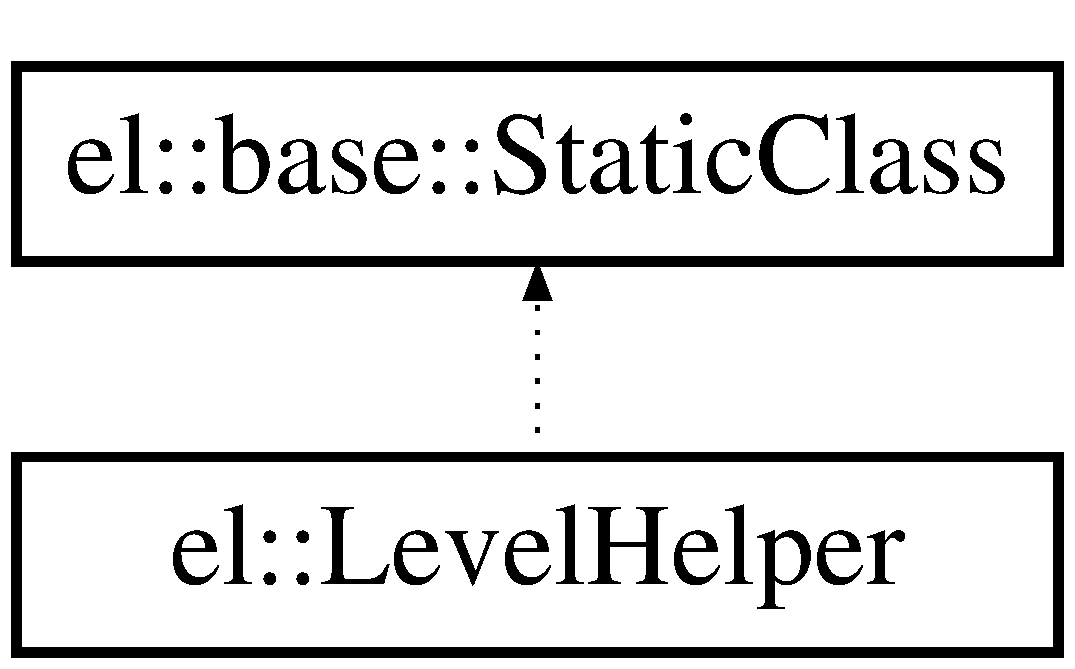
\includegraphics[height=2.000000cm]{classel_1_1_level_helper}
\end{center}
\end{figure}
\subsection*{Static Public Member Functions}
\begin{DoxyCompactItemize}
\item 
static \hyperlink{namespaceel_1_1base_1_1type_afb892a99b7545bf6e45c1e1d84af2ec9}{base\+::type\+::\+Enum\+Type} \hyperlink{classel_1_1_level_helper_a6576fd7cd6d1d839952145115c6e4b38}{cast\+To\+Int} (\hyperlink{namespaceel_ab0ac6091262344c52dd2d3ad099e8e36}{Level} level)
\begin{DoxyCompactList}\small\item\em Casts level to int, useful for iterating through enum. \end{DoxyCompactList}\item 
static \hyperlink{namespaceel_ab0ac6091262344c52dd2d3ad099e8e36}{Level} \hyperlink{classel_1_1_level_helper_a1279f27df29a003df5ecc3d0bf4dacbb}{cast\+From\+Int} (\hyperlink{namespaceel_1_1base_1_1type_afb892a99b7545bf6e45c1e1d84af2ec9}{base\+::type\+::\+Enum\+Type} l)
\begin{DoxyCompactList}\small\item\em Casts int(ushort) to level, useful for iterating through enum. \end{DoxyCompactList}\item 
static const char $\ast$ \hyperlink{classel_1_1_level_helper_a53b3e226a09af6e87c2072c115b3ba1a}{convert\+To\+String} (\hyperlink{namespaceel_ab0ac6091262344c52dd2d3ad099e8e36}{Level} level)
\begin{DoxyCompactList}\small\item\em Converts level to associated const char$\ast$. \end{DoxyCompactList}\item 
static \hyperlink{namespaceel_ab0ac6091262344c52dd2d3ad099e8e36}{Level} \hyperlink{classel_1_1_level_helper_a4ff401c62931609c849d580fb6ad2028}{convert\+From\+String} (const char $\ast$level\+Str)
\begin{DoxyCompactList}\small\item\em Converts from level\+Str to Level. \end{DoxyCompactList}\item 
static void \hyperlink{classel_1_1_level_helper_a94449b79778145f4c58fd1da6bcaf45d}{for\+Each\+Level} (\hyperlink{namespaceel_1_1base_1_1type_afb892a99b7545bf6e45c1e1d84af2ec9}{base\+::type\+::\+Enum\+Type} $\ast$start\+Index, const std\+::function$<$ bool(void)$>$ \&fn)
\begin{DoxyCompactList}\small\item\em Applies specified function to each level starting from start\+Index. \end{DoxyCompactList}\end{DoxyCompactItemize}
\subsection*{Static Public Attributes}
\begin{DoxyCompactItemize}
\item 
static const \hyperlink{namespaceel_1_1base_1_1type_afb892a99b7545bf6e45c1e1d84af2ec9}{base\+::type\+::\+Enum\+Type} \hyperlink{classel_1_1_level_helper_a3ecfe43d5b242e9946bad7f61ea4d89d}{k\+Min\+Valid} = static\+\_\+cast$<$\hyperlink{namespaceel_1_1base_1_1type_afb892a99b7545bf6e45c1e1d84af2ec9}{base\+::type\+::\+Enum\+Type}$>$(\hyperlink{namespaceel_ab0ac6091262344c52dd2d3ad099e8e36add4ec0ac4e58f7c32a01244ae91150b1}{Level\+::\+Trace})
\begin{DoxyCompactList}\small\item\em Represents minimum valid level. Useful when iterating through enum. \end{DoxyCompactList}\item 
static const \hyperlink{namespaceel_1_1base_1_1type_afb892a99b7545bf6e45c1e1d84af2ec9}{base\+::type\+::\+Enum\+Type} \hyperlink{classel_1_1_level_helper_aa06e80c65db5c336c4aad25872cf9a48}{k\+Max\+Valid} = static\+\_\+cast$<$\hyperlink{namespaceel_1_1base_1_1type_afb892a99b7545bf6e45c1e1d84af2ec9}{base\+::type\+::\+Enum\+Type}$>$(\hyperlink{namespaceel_ab0ac6091262344c52dd2d3ad099e8e36a4059b0251f66a18cb56f544728796875}{Level\+::\+Info})
\begin{DoxyCompactList}\small\item\em Represents maximum valid level. This is used internally and you should not need it. \end{DoxyCompactList}\end{DoxyCompactItemize}


\subsection{Detailed Description}
Static class that contains helper functions for \hyperlink{namespaceel_ab0ac6091262344c52dd2d3ad099e8e36}{el\+::\+Level}. 

Definition at line 523 of file easylogging++.\+h.



\subsection{Member Function Documentation}
\hypertarget{classel_1_1_level_helper_a1279f27df29a003df5ecc3d0bf4dacbb}{}\index{el\+::\+Level\+Helper@{el\+::\+Level\+Helper}!cast\+From\+Int@{cast\+From\+Int}}
\index{cast\+From\+Int@{cast\+From\+Int}!el\+::\+Level\+Helper@{el\+::\+Level\+Helper}}
\subsubsection[{cast\+From\+Int}]{\setlength{\rightskip}{0pt plus 5cm}static {\bf Level} el\+::\+Level\+Helper\+::cast\+From\+Int (
\begin{DoxyParamCaption}
\item[{{\bf base\+::type\+::\+Enum\+Type}}]{l}
\end{DoxyParamCaption}
)\hspace{0.3cm}{\ttfamily [inline]}, {\ttfamily [static]}}\label{classel_1_1_level_helper_a1279f27df29a003df5ecc3d0bf4dacbb}


Casts int(ushort) to level, useful for iterating through enum. 



Definition at line 534 of file easylogging++.\+h.

\hypertarget{classel_1_1_level_helper_a6576fd7cd6d1d839952145115c6e4b38}{}\index{el\+::\+Level\+Helper@{el\+::\+Level\+Helper}!cast\+To\+Int@{cast\+To\+Int}}
\index{cast\+To\+Int@{cast\+To\+Int}!el\+::\+Level\+Helper@{el\+::\+Level\+Helper}}
\subsubsection[{cast\+To\+Int}]{\setlength{\rightskip}{0pt plus 5cm}static {\bf base\+::type\+::\+Enum\+Type} el\+::\+Level\+Helper\+::cast\+To\+Int (
\begin{DoxyParamCaption}
\item[{{\bf Level}}]{level}
\end{DoxyParamCaption}
)\hspace{0.3cm}{\ttfamily [inline]}, {\ttfamily [static]}}\label{classel_1_1_level_helper_a6576fd7cd6d1d839952145115c6e4b38}


Casts level to int, useful for iterating through enum. 



Definition at line 530 of file easylogging++.\+h.

\hypertarget{classel_1_1_level_helper_a4ff401c62931609c849d580fb6ad2028}{}\index{el\+::\+Level\+Helper@{el\+::\+Level\+Helper}!convert\+From\+String@{convert\+From\+String}}
\index{convert\+From\+String@{convert\+From\+String}!el\+::\+Level\+Helper@{el\+::\+Level\+Helper}}
\subsubsection[{convert\+From\+String}]{\setlength{\rightskip}{0pt plus 5cm}static {\bf Level} el\+::\+Level\+Helper\+::convert\+From\+String (
\begin{DoxyParamCaption}
\item[{const char $\ast$}]{level\+Str}
\end{DoxyParamCaption}
)\hspace{0.3cm}{\ttfamily [inline]}, {\ttfamily [static]}}\label{classel_1_1_level_helper_a4ff401c62931609c849d580fb6ad2028}


Converts from level\+Str to Level. 


\begin{DoxyParams}{Parameters}
{\em level\+Str} & Upper case string based level. Lower case is also valid but providing upper case is recommended. \\
\hline
\end{DoxyParams}


Definition at line 554 of file easylogging++.\+h.

\hypertarget{classel_1_1_level_helper_a53b3e226a09af6e87c2072c115b3ba1a}{}\index{el\+::\+Level\+Helper@{el\+::\+Level\+Helper}!convert\+To\+String@{convert\+To\+String}}
\index{convert\+To\+String@{convert\+To\+String}!el\+::\+Level\+Helper@{el\+::\+Level\+Helper}}
\subsubsection[{convert\+To\+String}]{\setlength{\rightskip}{0pt plus 5cm}static const char$\ast$ el\+::\+Level\+Helper\+::convert\+To\+String (
\begin{DoxyParamCaption}
\item[{{\bf Level}}]{level}
\end{DoxyParamCaption}
)\hspace{0.3cm}{\ttfamily [inline]}, {\ttfamily [static]}}\label{classel_1_1_level_helper_a53b3e226a09af6e87c2072c115b3ba1a}


Converts level to associated const char$\ast$. 

\begin{DoxyReturn}{Returns}
Upper case string based level. 
\end{DoxyReturn}


Definition at line 539 of file easylogging++.\+h.

\hypertarget{classel_1_1_level_helper_a94449b79778145f4c58fd1da6bcaf45d}{}\index{el\+::\+Level\+Helper@{el\+::\+Level\+Helper}!for\+Each\+Level@{for\+Each\+Level}}
\index{for\+Each\+Level@{for\+Each\+Level}!el\+::\+Level\+Helper@{el\+::\+Level\+Helper}}
\subsubsection[{for\+Each\+Level}]{\setlength{\rightskip}{0pt plus 5cm}static void el\+::\+Level\+Helper\+::for\+Each\+Level (
\begin{DoxyParamCaption}
\item[{{\bf base\+::type\+::\+Enum\+Type} $\ast$}]{start\+Index, }
\item[{const std\+::function$<$ bool(void)$>$ \&}]{fn}
\end{DoxyParamCaption}
)\hspace{0.3cm}{\ttfamily [inline]}, {\ttfamily [static]}}\label{classel_1_1_level_helper_a94449b79778145f4c58fd1da6bcaf45d}


Applies specified function to each level starting from start\+Index. 


\begin{DoxyParams}{Parameters}
{\em start\+Index} & initial value to start the iteration from. This is passed as pointer and is left-\/shifted so this can be used inside function (fn) to represent current level. \\
\hline
{\em fn} & function to apply with each level. This bool represent whether or not to stop iterating through levels. \\
\hline
\end{DoxyParams}


Definition at line 577 of file easylogging++.\+h.



\subsection{Member Data Documentation}
\hypertarget{classel_1_1_level_helper_aa06e80c65db5c336c4aad25872cf9a48}{}\index{el\+::\+Level\+Helper@{el\+::\+Level\+Helper}!k\+Max\+Valid@{k\+Max\+Valid}}
\index{k\+Max\+Valid@{k\+Max\+Valid}!el\+::\+Level\+Helper@{el\+::\+Level\+Helper}}
\subsubsection[{k\+Max\+Valid}]{\setlength{\rightskip}{0pt plus 5cm}const {\bf base\+::type\+::\+Enum\+Type} el\+::\+Level\+Helper\+::k\+Max\+Valid = static\+\_\+cast$<${\bf base\+::type\+::\+Enum\+Type}$>$({\bf Level\+::\+Info})\hspace{0.3cm}{\ttfamily [static]}}\label{classel_1_1_level_helper_aa06e80c65db5c336c4aad25872cf9a48}


Represents maximum valid level. This is used internally and you should not need it. 



Definition at line 528 of file easylogging++.\+h.

\hypertarget{classel_1_1_level_helper_a3ecfe43d5b242e9946bad7f61ea4d89d}{}\index{el\+::\+Level\+Helper@{el\+::\+Level\+Helper}!k\+Min\+Valid@{k\+Min\+Valid}}
\index{k\+Min\+Valid@{k\+Min\+Valid}!el\+::\+Level\+Helper@{el\+::\+Level\+Helper}}
\subsubsection[{k\+Min\+Valid}]{\setlength{\rightskip}{0pt plus 5cm}const {\bf base\+::type\+::\+Enum\+Type} el\+::\+Level\+Helper\+::k\+Min\+Valid = static\+\_\+cast$<${\bf base\+::type\+::\+Enum\+Type}$>$({\bf Level\+::\+Trace})\hspace{0.3cm}{\ttfamily [static]}}\label{classel_1_1_level_helper_a3ecfe43d5b242e9946bad7f61ea4d89d}


Represents minimum valid level. Useful when iterating through enum. 



Definition at line 526 of file easylogging++.\+h.



The documentation for this class was generated from the following file\+:\begin{DoxyCompactItemize}
\item 
lib/\hyperlink{easylogging_09_09_8h}{easylogging++.\+h}\end{DoxyCompactItemize}

\hypertarget{class_l_i_f_o}{}\section{L\+I\+F\+O Class Reference}
\label{class_l_i_f_o}\index{L\+I\+F\+O@{L\+I\+F\+O}}


{\ttfamily \#include $<$L\+I\+F\+O.\+h$>$}

Inheritance diagram for L\+I\+F\+O\+:\begin{figure}[H]
\begin{center}
\leavevmode
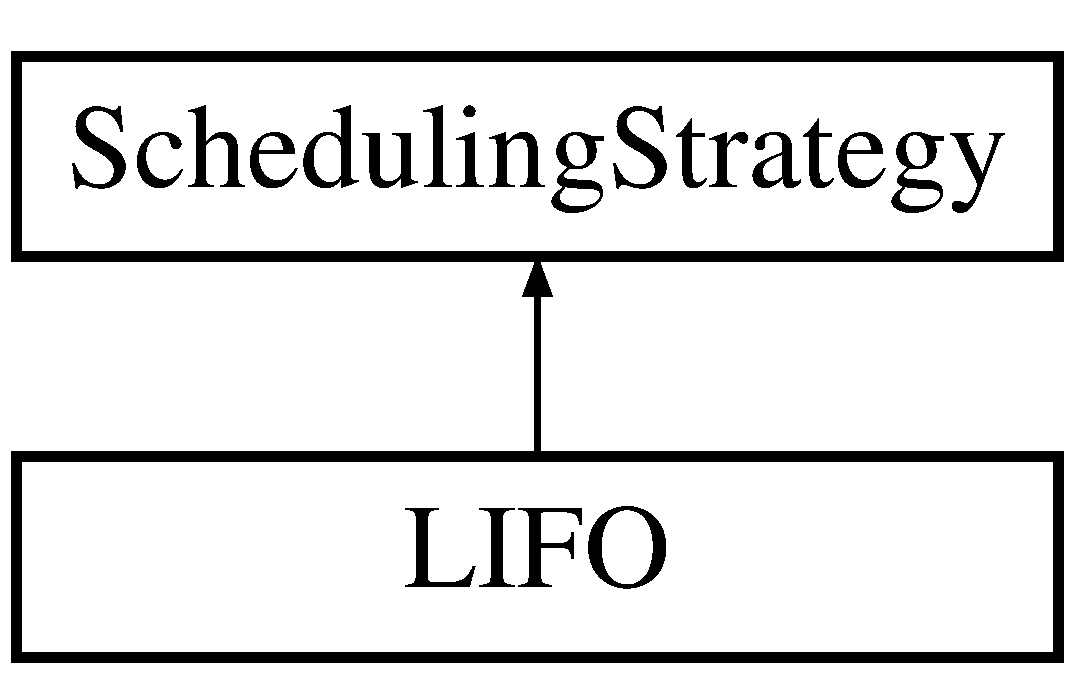
\includegraphics[height=2.000000cm]{class_l_i_f_o}
\end{center}
\end{figure}
\subsection*{Public Member Functions}
\begin{DoxyCompactItemize}
\item 
\hyperlink{class_l_i_f_o_a594555175f097e6cf98db278d695dd6f}{L\+I\+F\+O} ()
\item 
\hyperlink{class_l_i_f_o_af8722c4d9d050eddf9e17714d5d90594}{$\sim$\+L\+I\+F\+O} ()
\item 
\hyperlink{_types_8h_a0c77930ab3818a1680c59353f627fba8}{Task} \hyperlink{class_l_i_f_o_a53eb12a8a25f0fb4f57679206bf314dc}{get\+\_\+next\+\_\+task} ()
\item 
int \hyperlink{class_l_i_f_o_a6368d6fe156688f38d06a0ee75d57ef6}{get\+\_\+task\+\_\+count} ()
\item 
\hyperlink{_types_8h_a0c77930ab3818a1680c59353f627fba8}{Task} \hyperlink{class_l_i_f_o_a1593c380d2f3f0e8f2247a2b61c9607c}{pop\+\_\+next\+\_\+task} ()
\item 
void \hyperlink{class_l_i_f_o_a422ac5b308521b23e97c25f7fc80ee7c}{push\+\_\+new\+\_\+task} (\hyperlink{_types_8h_a0c77930ab3818a1680c59353f627fba8}{Task} task, long runtime)
\item 
\hyperlink{class_scheduling_strategy}{Scheduling\+Strategy} $\ast$ \hyperlink{class_l_i_f_o_a6e3553527c29e2c90bf86d4a4e5cd570}{change\+\_\+strategy} (\hyperlink{class_scheduling_strategy}{Scheduling\+Strategy} $\ast$new\+\_\+strategy)
\item 
bool \hyperlink{class_l_i_f_o_a8a8a3203290cda8521b74acde5fc334d}{is\+\_\+statistic\+\_\+based} ()
\end{DoxyCompactItemize}
\subsection*{Additional Inherited Members}


\subsection{Detailed Description}
This class realize the last in-\/first out (\hyperlink{class_l_i_f_o}{L\+I\+F\+O}) scheduling strategy. The \hyperlink{class_l_i_f_o}{L\+I\+F\+O} class uses the std\+::stack as fifo queue.

\begin{DoxyAuthor}{Author}
Fabio Broghammer 
\end{DoxyAuthor}
\begin{DoxyVersion}{Version}
1.\+0 
\end{DoxyVersion}


Definition at line 16 of file L\+I\+F\+O.\+h.



\subsection{Constructor \& Destructor Documentation}
\hypertarget{class_l_i_f_o_a594555175f097e6cf98db278d695dd6f}{}\index{L\+I\+F\+O@{L\+I\+F\+O}!L\+I\+F\+O@{L\+I\+F\+O}}
\index{L\+I\+F\+O@{L\+I\+F\+O}!L\+I\+F\+O@{L\+I\+F\+O}}
\subsubsection[{L\+I\+F\+O}]{\setlength{\rightskip}{0pt plus 5cm}L\+I\+F\+O\+::\+L\+I\+F\+O (
\begin{DoxyParamCaption}
{}
\end{DoxyParamCaption}
)}\label{class_l_i_f_o_a594555175f097e6cf98db278d695dd6f}
Constructs a new \hyperlink{class_l_i_f_o}{L\+I\+F\+O} scheduling queue 

Definition at line 6 of file L\+I\+F\+O.\+cpp.

\hypertarget{class_l_i_f_o_af8722c4d9d050eddf9e17714d5d90594}{}\index{L\+I\+F\+O@{L\+I\+F\+O}!````~L\+I\+F\+O@{$\sim$\+L\+I\+F\+O}}
\index{````~L\+I\+F\+O@{$\sim$\+L\+I\+F\+O}!L\+I\+F\+O@{L\+I\+F\+O}}
\subsubsection[{$\sim$\+L\+I\+F\+O}]{\setlength{\rightskip}{0pt plus 5cm}L\+I\+F\+O\+::$\sim$\+L\+I\+F\+O (
\begin{DoxyParamCaption}
{}
\end{DoxyParamCaption}
)}\label{class_l_i_f_o_af8722c4d9d050eddf9e17714d5d90594}
Destructs a new \hyperlink{class_l_i_f_o}{L\+I\+F\+O} scheduling queue 

Definition at line 11 of file L\+I\+F\+O.\+cpp.



\subsection{Member Function Documentation}
\hypertarget{class_l_i_f_o_a6e3553527c29e2c90bf86d4a4e5cd570}{}\index{L\+I\+F\+O@{L\+I\+F\+O}!change\+\_\+strategy@{change\+\_\+strategy}}
\index{change\+\_\+strategy@{change\+\_\+strategy}!L\+I\+F\+O@{L\+I\+F\+O}}
\subsubsection[{change\+\_\+strategy}]{\setlength{\rightskip}{0pt plus 5cm}{\bf Scheduling\+Strategy} $\ast$ L\+I\+F\+O\+::change\+\_\+strategy (
\begin{DoxyParamCaption}
\item[{{\bf Scheduling\+Strategy} $\ast$}]{new\+\_\+strategy}
\end{DoxyParamCaption}
)\hspace{0.3cm}{\ttfamily [virtual]}}\label{class_l_i_f_o_a6e3553527c29e2c90bf86d4a4e5cd570}
Changes the scheduling strategy. Returns the new schdeuling strategy with all tasks, or N\+U\+L\+L if there was an error.

Estimated runtime of tasks will get lost by changing from statistically based strategies (L\+S\+F, \hyperlink{class_s_j_f}{S\+J\+F}) to non-\/statistically based strategies. The order of the old queue will be kept.

All tasks will get a default rumtime value (defined in D\+E\+F\+A\+U\+L\+T\+\_\+\+R\+U\+N\+T\+I\+M\+E) by changing from non-\/statistically based strategies (\hyperlink{class_f_i_f_o}{F\+I\+F\+O}, \hyperlink{class_l_i_f_o}{L\+I\+F\+O}) to statistically based strategies. The order of the old queue perhaps won\textquotesingle{}t be kept 
\begin{DoxyParams}{Parameters}
{\em new\+\_\+strategy} & \\
\hline
\end{DoxyParams}


Implements \hyperlink{class_scheduling_strategy_a4874d194c1bb185480339360fe907d83}{Scheduling\+Strategy}.



Definition at line 40 of file L\+I\+F\+O.\+cpp.

\hypertarget{class_l_i_f_o_a53eb12a8a25f0fb4f57679206bf314dc}{}\index{L\+I\+F\+O@{L\+I\+F\+O}!get\+\_\+next\+\_\+task@{get\+\_\+next\+\_\+task}}
\index{get\+\_\+next\+\_\+task@{get\+\_\+next\+\_\+task}!L\+I\+F\+O@{L\+I\+F\+O}}
\subsubsection[{get\+\_\+next\+\_\+task}]{\setlength{\rightskip}{0pt plus 5cm}{\bf Task} L\+I\+F\+O\+::get\+\_\+next\+\_\+task (
\begin{DoxyParamCaption}
{}
\end{DoxyParamCaption}
)\hspace{0.3cm}{\ttfamily [virtual]}}\label{class_l_i_f_o_a53eb12a8a25f0fb4f57679206bf314dc}
Returns the last-\/in task, or N\+U\+L\+L if the queue is empty

\begin{DoxyReturn}{Returns}
the last-\/in task 
\end{DoxyReturn}


Implements \hyperlink{class_scheduling_strategy_adce3619801460ad67d6c8f9bdffcd36b}{Scheduling\+Strategy}.



Definition at line 17 of file L\+I\+F\+O.\+cpp.

\hypertarget{class_l_i_f_o_a6368d6fe156688f38d06a0ee75d57ef6}{}\index{L\+I\+F\+O@{L\+I\+F\+O}!get\+\_\+task\+\_\+count@{get\+\_\+task\+\_\+count}}
\index{get\+\_\+task\+\_\+count@{get\+\_\+task\+\_\+count}!L\+I\+F\+O@{L\+I\+F\+O}}
\subsubsection[{get\+\_\+task\+\_\+count}]{\setlength{\rightskip}{0pt plus 5cm}int L\+I\+F\+O\+::get\+\_\+task\+\_\+count (
\begin{DoxyParamCaption}
{}
\end{DoxyParamCaption}
)\hspace{0.3cm}{\ttfamily [virtual]}}\label{class_l_i_f_o_a6368d6fe156688f38d06a0ee75d57ef6}
Return the count of tasks in the scheduling queue

the count of tasks 

Implements \hyperlink{class_scheduling_strategy_a0a3355ffe9c03236692ad00e4f94f5c5}{Scheduling\+Strategy}.



Definition at line 22 of file L\+I\+F\+O.\+cpp.

\hypertarget{class_l_i_f_o_a8a8a3203290cda8521b74acde5fc334d}{}\index{L\+I\+F\+O@{L\+I\+F\+O}!is\+\_\+statistic\+\_\+based@{is\+\_\+statistic\+\_\+based}}
\index{is\+\_\+statistic\+\_\+based@{is\+\_\+statistic\+\_\+based}!L\+I\+F\+O@{L\+I\+F\+O}}
\subsubsection[{is\+\_\+statistic\+\_\+based}]{\setlength{\rightskip}{0pt plus 5cm}bool L\+I\+F\+O\+::is\+\_\+statistic\+\_\+based (
\begin{DoxyParamCaption}
{}
\end{DoxyParamCaption}
)\hspace{0.3cm}{\ttfamily [virtual]}}\label{class_l_i_f_o_a8a8a3203290cda8521b74acde5fc334d}
Returns true, if the current scheduling strategy statistic based.

\begin{DoxyReturn}{Returns}
true, if the current scheduling strategy statistic based 
\end{DoxyReturn}


Implements \hyperlink{class_scheduling_strategy_a5962845ca5af53bbdc014c19a6bdef99}{Scheduling\+Strategy}.



Definition at line 50 of file L\+I\+F\+O.\+cpp.

\hypertarget{class_l_i_f_o_a1593c380d2f3f0e8f2247a2b61c9607c}{}\index{L\+I\+F\+O@{L\+I\+F\+O}!pop\+\_\+next\+\_\+task@{pop\+\_\+next\+\_\+task}}
\index{pop\+\_\+next\+\_\+task@{pop\+\_\+next\+\_\+task}!L\+I\+F\+O@{L\+I\+F\+O}}
\subsubsection[{pop\+\_\+next\+\_\+task}]{\setlength{\rightskip}{0pt plus 5cm}{\bf Task} L\+I\+F\+O\+::pop\+\_\+next\+\_\+task (
\begin{DoxyParamCaption}
{}
\end{DoxyParamCaption}
)\hspace{0.3cm}{\ttfamily [virtual]}}\label{class_l_i_f_o_a1593c380d2f3f0e8f2247a2b61c9607c}
Removes the next task in the queue, effectively reducing its size by one. 

Implements \hyperlink{class_scheduling_strategy_ac2ba483287c91fd4318f337da144a9c5}{Scheduling\+Strategy}.



Definition at line 27 of file L\+I\+F\+O.\+cpp.

\hypertarget{class_l_i_f_o_a422ac5b308521b23e97c25f7fc80ee7c}{}\index{L\+I\+F\+O@{L\+I\+F\+O}!push\+\_\+new\+\_\+task@{push\+\_\+new\+\_\+task}}
\index{push\+\_\+new\+\_\+task@{push\+\_\+new\+\_\+task}!L\+I\+F\+O@{L\+I\+F\+O}}
\subsubsection[{push\+\_\+new\+\_\+task}]{\setlength{\rightskip}{0pt plus 5cm}void L\+I\+F\+O\+::push\+\_\+new\+\_\+task (
\begin{DoxyParamCaption}
\item[{{\bf Task}}]{task, }
\item[{long}]{runtime}
\end{DoxyParamCaption}
)\hspace{0.3cm}{\ttfamily [virtual]}}\label{class_l_i_f_o_a422ac5b308521b23e97c25f7fc80ee7c}
Insert a new task in the scheduling queue depending on the scheduling strategy and the estimated runtime 
\begin{DoxyParams}{Parameters}
{\em task} & \\
\hline
{\em runtime} & \\
\hline
\end{DoxyParams}


Implements \hyperlink{class_scheduling_strategy_a62ffa0426528c14fdd0b0853f04a851f}{Scheduling\+Strategy}.



Definition at line 35 of file L\+I\+F\+O.\+cpp.



The documentation for this class was generated from the following files\+:\begin{DoxyCompactItemize}
\item 
src/scheduler/\hyperlink{_l_i_f_o_8h}{L\+I\+F\+O.\+h}\item 
src/scheduler/\hyperlink{_l_i_f_o_8cpp}{L\+I\+F\+O.\+cpp}\end{DoxyCompactItemize}

\hypertarget{class_l_i_f_o_test_case}{}\section{L\+I\+F\+O\+Test\+Case Class Reference}
\label{class_l_i_f_o_test_case}\index{L\+I\+F\+O\+Test\+Case@{L\+I\+F\+O\+Test\+Case}}


{\ttfamily \#include $<$L\+I\+F\+O\+Test\+Case.\+h$>$}

Inheritance diagram for L\+I\+F\+O\+Test\+Case\+:\begin{figure}[H]
\begin{center}
\leavevmode
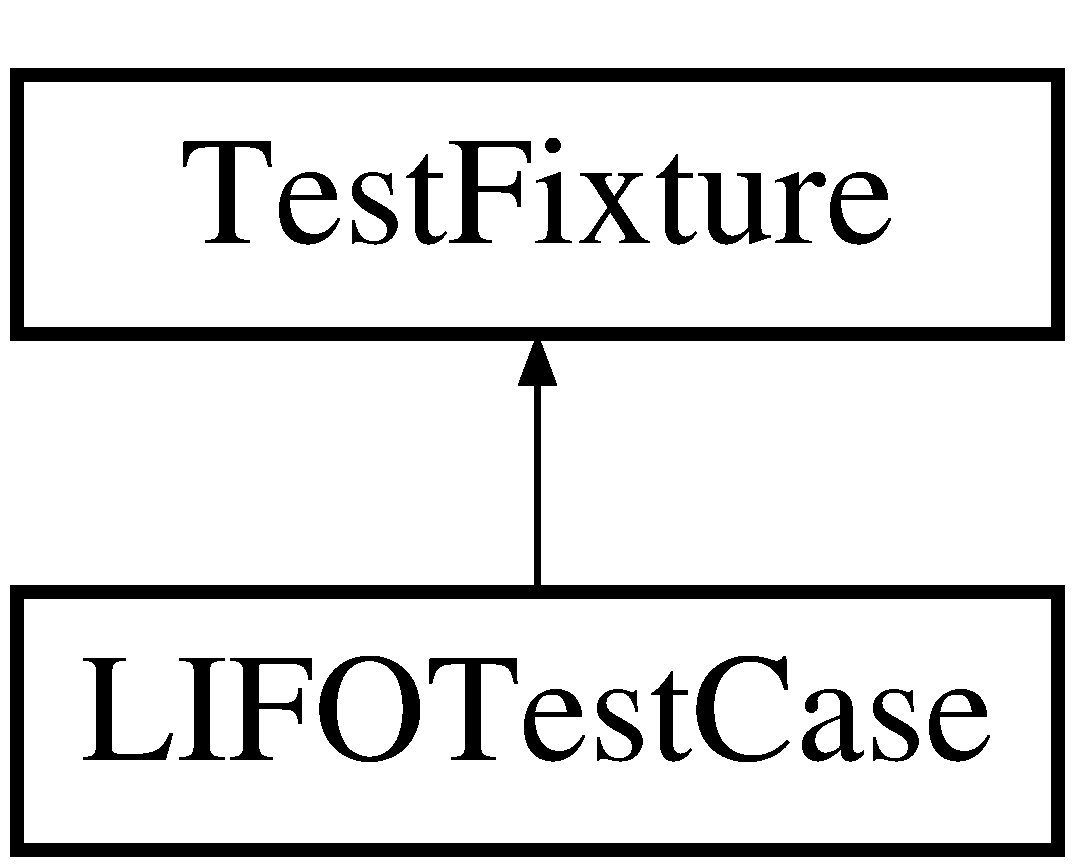
\includegraphics[height=2.000000cm]{class_l_i_f_o_test_case}
\end{center}
\end{figure}
\subsection*{Public Member Functions}
\begin{DoxyCompactItemize}
\item 
void \hyperlink{class_l_i_f_o_test_case_a4a028862ef1179061435da3ca058670e}{set\+Up} ()
\item 
void \hyperlink{class_l_i_f_o_test_case_aa83dba5d549606eba6a54cce4f21c52e}{tear\+Down} ()
\item 
void \hyperlink{class_l_i_f_o_test_case_a99cbee000f0fb1ab639d7bd69faeca06}{test\+\_\+pop\+\_\+task} ()
\item 
void \hyperlink{class_l_i_f_o_test_case_af5481343cc459b8f16618d13314ecdc0}{test\+\_\+push\+\_\+new\+\_\+task} ()
\item 
void \hyperlink{class_l_i_f_o_test_case_aa9073edb510daef4051de7e76b27d6ec}{test\+\_\+is\+\_\+statistic\+\_\+based} ()
\item 
void \hyperlink{class_l_i_f_o_test_case_af7883d3964f2e57802cee6b14be48bb4}{test\+\_\+get\+\_\+count} ()
\item 
void \hyperlink{class_l_i_f_o_test_case_a30a895909a806d006c59bdaae9f1a1c9}{test\+\_\+get\+\_\+next\+\_\+task} ()
\end{DoxyCompactItemize}
\subsection*{Static Public Member Functions}
\begin{DoxyCompactItemize}
\item 
static Test $\ast$ \hyperlink{class_l_i_f_o_test_case_a0bd464ab76c423a53368ebf25577af8e}{suite} ()
\end{DoxyCompactItemize}


\subsection{Detailed Description}


Definition at line 24 of file L\+I\+F\+O\+Test\+Case.\+h.



\subsection{Member Function Documentation}
\hypertarget{class_l_i_f_o_test_case_a4a028862ef1179061435da3ca058670e}{}\index{L\+I\+F\+O\+Test\+Case@{L\+I\+F\+O\+Test\+Case}!set\+Up@{set\+Up}}
\index{set\+Up@{set\+Up}!L\+I\+F\+O\+Test\+Case@{L\+I\+F\+O\+Test\+Case}}
\subsubsection[{set\+Up}]{\setlength{\rightskip}{0pt plus 5cm}void L\+I\+F\+O\+Test\+Case\+::set\+Up (
\begin{DoxyParamCaption}
{}
\end{DoxyParamCaption}
)}\label{class_l_i_f_o_test_case_a4a028862ef1179061435da3ca058670e}


Definition at line 30 of file L\+I\+F\+O\+Test\+Case.\+cpp.

\hypertarget{class_l_i_f_o_test_case_a0bd464ab76c423a53368ebf25577af8e}{}\index{L\+I\+F\+O\+Test\+Case@{L\+I\+F\+O\+Test\+Case}!suite@{suite}}
\index{suite@{suite}!L\+I\+F\+O\+Test\+Case@{L\+I\+F\+O\+Test\+Case}}
\subsubsection[{suite}]{\setlength{\rightskip}{0pt plus 5cm}Test $\ast$ L\+I\+F\+O\+Test\+Case\+::suite (
\begin{DoxyParamCaption}
{}
\end{DoxyParamCaption}
)\hspace{0.3cm}{\ttfamily [static]}}\label{class_l_i_f_o_test_case_a0bd464ab76c423a53368ebf25577af8e}


Definition at line 19 of file L\+I\+F\+O\+Test\+Case.\+cpp.

\hypertarget{class_l_i_f_o_test_case_aa83dba5d549606eba6a54cce4f21c52e}{}\index{L\+I\+F\+O\+Test\+Case@{L\+I\+F\+O\+Test\+Case}!tear\+Down@{tear\+Down}}
\index{tear\+Down@{tear\+Down}!L\+I\+F\+O\+Test\+Case@{L\+I\+F\+O\+Test\+Case}}
\subsubsection[{tear\+Down}]{\setlength{\rightskip}{0pt plus 5cm}void L\+I\+F\+O\+Test\+Case\+::tear\+Down (
\begin{DoxyParamCaption}
{}
\end{DoxyParamCaption}
)}\label{class_l_i_f_o_test_case_aa83dba5d549606eba6a54cce4f21c52e}


Definition at line 34 of file L\+I\+F\+O\+Test\+Case.\+cpp.

\hypertarget{class_l_i_f_o_test_case_af7883d3964f2e57802cee6b14be48bb4}{}\index{L\+I\+F\+O\+Test\+Case@{L\+I\+F\+O\+Test\+Case}!test\+\_\+get\+\_\+count@{test\+\_\+get\+\_\+count}}
\index{test\+\_\+get\+\_\+count@{test\+\_\+get\+\_\+count}!L\+I\+F\+O\+Test\+Case@{L\+I\+F\+O\+Test\+Case}}
\subsubsection[{test\+\_\+get\+\_\+count}]{\setlength{\rightskip}{0pt plus 5cm}void L\+I\+F\+O\+Test\+Case\+::test\+\_\+get\+\_\+count (
\begin{DoxyParamCaption}
{}
\end{DoxyParamCaption}
)}\label{class_l_i_f_o_test_case_af7883d3964f2e57802cee6b14be48bb4}


Definition at line 42 of file L\+I\+F\+O\+Test\+Case.\+cpp.

\hypertarget{class_l_i_f_o_test_case_a30a895909a806d006c59bdaae9f1a1c9}{}\index{L\+I\+F\+O\+Test\+Case@{L\+I\+F\+O\+Test\+Case}!test\+\_\+get\+\_\+next\+\_\+task@{test\+\_\+get\+\_\+next\+\_\+task}}
\index{test\+\_\+get\+\_\+next\+\_\+task@{test\+\_\+get\+\_\+next\+\_\+task}!L\+I\+F\+O\+Test\+Case@{L\+I\+F\+O\+Test\+Case}}
\subsubsection[{test\+\_\+get\+\_\+next\+\_\+task}]{\setlength{\rightskip}{0pt plus 5cm}void L\+I\+F\+O\+Test\+Case\+::test\+\_\+get\+\_\+next\+\_\+task (
\begin{DoxyParamCaption}
{}
\end{DoxyParamCaption}
)}\label{class_l_i_f_o_test_case_a30a895909a806d006c59bdaae9f1a1c9}


Definition at line 79 of file L\+I\+F\+O\+Test\+Case.\+cpp.

\hypertarget{class_l_i_f_o_test_case_aa9073edb510daef4051de7e76b27d6ec}{}\index{L\+I\+F\+O\+Test\+Case@{L\+I\+F\+O\+Test\+Case}!test\+\_\+is\+\_\+statistic\+\_\+based@{test\+\_\+is\+\_\+statistic\+\_\+based}}
\index{test\+\_\+is\+\_\+statistic\+\_\+based@{test\+\_\+is\+\_\+statistic\+\_\+based}!L\+I\+F\+O\+Test\+Case@{L\+I\+F\+O\+Test\+Case}}
\subsubsection[{test\+\_\+is\+\_\+statistic\+\_\+based}]{\setlength{\rightskip}{0pt plus 5cm}void L\+I\+F\+O\+Test\+Case\+::test\+\_\+is\+\_\+statistic\+\_\+based (
\begin{DoxyParamCaption}
{}
\end{DoxyParamCaption}
)}\label{class_l_i_f_o_test_case_aa9073edb510daef4051de7e76b27d6ec}


Definition at line 38 of file L\+I\+F\+O\+Test\+Case.\+cpp.

\hypertarget{class_l_i_f_o_test_case_a99cbee000f0fb1ab639d7bd69faeca06}{}\index{L\+I\+F\+O\+Test\+Case@{L\+I\+F\+O\+Test\+Case}!test\+\_\+pop\+\_\+task@{test\+\_\+pop\+\_\+task}}
\index{test\+\_\+pop\+\_\+task@{test\+\_\+pop\+\_\+task}!L\+I\+F\+O\+Test\+Case@{L\+I\+F\+O\+Test\+Case}}
\subsubsection[{test\+\_\+pop\+\_\+task}]{\setlength{\rightskip}{0pt plus 5cm}void L\+I\+F\+O\+Test\+Case\+::test\+\_\+pop\+\_\+task (
\begin{DoxyParamCaption}
{}
\end{DoxyParamCaption}
)}\label{class_l_i_f_o_test_case_a99cbee000f0fb1ab639d7bd69faeca06}


Definition at line 53 of file L\+I\+F\+O\+Test\+Case.\+cpp.

\hypertarget{class_l_i_f_o_test_case_af5481343cc459b8f16618d13314ecdc0}{}\index{L\+I\+F\+O\+Test\+Case@{L\+I\+F\+O\+Test\+Case}!test\+\_\+push\+\_\+new\+\_\+task@{test\+\_\+push\+\_\+new\+\_\+task}}
\index{test\+\_\+push\+\_\+new\+\_\+task@{test\+\_\+push\+\_\+new\+\_\+task}!L\+I\+F\+O\+Test\+Case@{L\+I\+F\+O\+Test\+Case}}
\subsubsection[{test\+\_\+push\+\_\+new\+\_\+task}]{\setlength{\rightskip}{0pt plus 5cm}void L\+I\+F\+O\+Test\+Case\+::test\+\_\+push\+\_\+new\+\_\+task (
\begin{DoxyParamCaption}
{}
\end{DoxyParamCaption}
)}\label{class_l_i_f_o_test_case_af5481343cc459b8f16618d13314ecdc0}


Definition at line 68 of file L\+I\+F\+O\+Test\+Case.\+cpp.



The documentation for this class was generated from the following files\+:\begin{DoxyCompactItemize}
\item 
test/scheduler/\hyperlink{_l_i_f_o_test_case_8h}{L\+I\+F\+O\+Test\+Case.\+h}\item 
test/scheduler/\hyperlink{_l_i_f_o_test_case_8cpp}{L\+I\+F\+O\+Test\+Case.\+cpp}\end{DoxyCompactItemize}

\hypertarget{class_l_j_f}{}\section{L\+J\+F Class Reference}
\label{class_l_j_f}\index{L\+J\+F@{L\+J\+F}}


{\ttfamily \#include $<$L\+J\+F.\+h$>$}

Inheritance diagram for L\+J\+F\+:\begin{figure}[H]
\begin{center}
\leavevmode
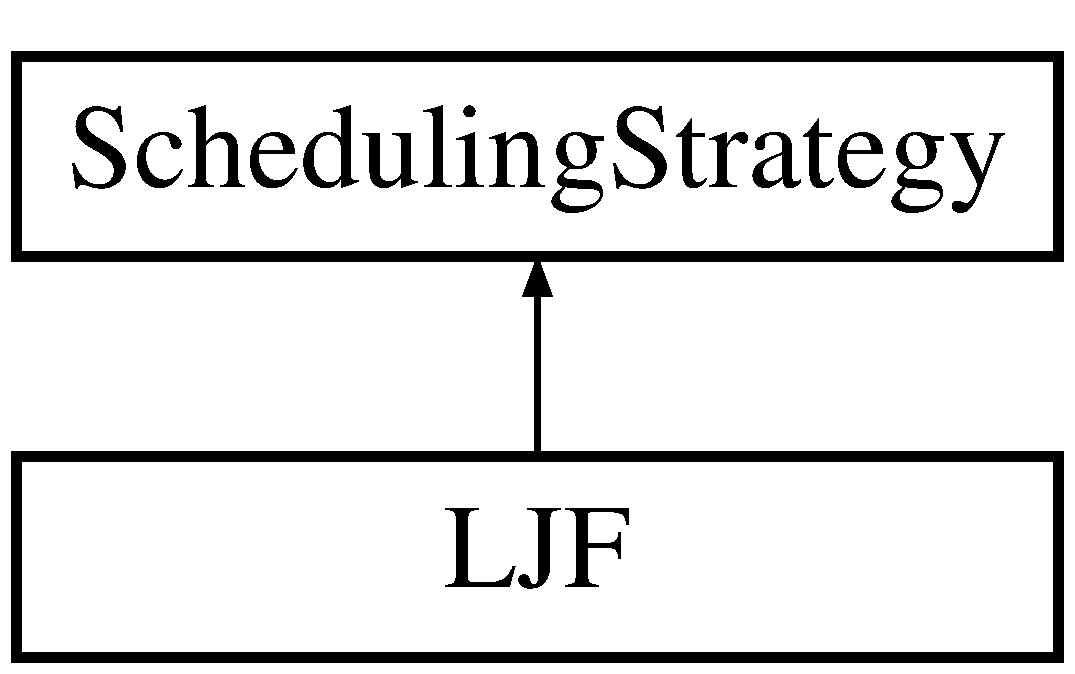
\includegraphics[height=2.000000cm]{class_l_j_f}
\end{center}
\end{figure}
\subsection*{Public Member Functions}
\begin{DoxyCompactItemize}
\item 
\hyperlink{class_l_j_f_ae8c4fa391d8767a5fba0bfb3ad3da8db}{L\+J\+F} ()
\item 
\hyperlink{class_l_j_f_a5ad18e75f4069623320bc72e3ec6e4ce}{$\sim$\+L\+J\+F} ()
\item 
\hyperlink{_types_8h_a0c77930ab3818a1680c59353f627fba8}{Task} \hyperlink{class_l_j_f_a24a4c6bfba65ef98753242c1f068b9fd}{get\+\_\+next\+\_\+task} ()
\item 
int \hyperlink{class_l_j_f_a329055147464eb68940c0541aba5946e}{get\+\_\+task\+\_\+count} ()
\item 
\hyperlink{_types_8h_a0c77930ab3818a1680c59353f627fba8}{Task} \hyperlink{class_l_j_f_af12a29f8a65fea1de0a2f436fd2b8b2b}{pop\+\_\+next\+\_\+task} ()
\item 
void \hyperlink{class_l_j_f_a4661c55d31322bc7755227890ca8679c}{push\+\_\+new\+\_\+task} (\hyperlink{_types_8h_a0c77930ab3818a1680c59353f627fba8}{Task} task, long runtime)
\item 
\hyperlink{class_scheduling_strategy}{Scheduling\+Strategy} $\ast$ \hyperlink{class_l_j_f_aaf5029dba4a8200d49f9b6bd47e71acd}{change\+\_\+strategy} (\hyperlink{class_scheduling_strategy}{Scheduling\+Strategy} $\ast$new\+\_\+strategy)
\item 
bool \hyperlink{class_l_j_f_a9292614934e9dc35f7c4ea568bcdcd4c}{is\+\_\+statistic\+\_\+based} ()
\end{DoxyCompactItemize}
\subsection*{Additional Inherited Members}


\subsection{Detailed Description}
This class implements the \hyperlink{class_scheduling_strategy}{Scheduling\+Strategy} interface and realises the Longest Job First (\hyperlink{class_l_j_f}{L\+J\+F}) scheduling strategy. Longest Job First scheduling uses the estimated runtime of tasks to order the task queue. \hyperlink{class_l_j_f}{L\+J\+F} is a statistically based scheduling strategy. The \hyperlink{class_l_j_f}{L\+J\+F} class uses the std\+::priority\+\_\+queue priority queue to keep the tasks.

\begin{DoxyAuthor}{Author}
Fabio Broghammer 
\end{DoxyAuthor}
\begin{DoxyVersion}{Version}
1.\+0 
\end{DoxyVersion}


Definition at line 37 of file L\+J\+F.\+h.



\subsection{Constructor \& Destructor Documentation}
\hypertarget{class_l_j_f_ae8c4fa391d8767a5fba0bfb3ad3da8db}{}\index{L\+J\+F@{L\+J\+F}!L\+J\+F@{L\+J\+F}}
\index{L\+J\+F@{L\+J\+F}!L\+J\+F@{L\+J\+F}}
\subsubsection[{L\+J\+F}]{\setlength{\rightskip}{0pt plus 5cm}L\+J\+F\+::\+L\+J\+F (
\begin{DoxyParamCaption}
{}
\end{DoxyParamCaption}
)}\label{class_l_j_f_ae8c4fa391d8767a5fba0bfb3ad3da8db}
Constructs a new \hyperlink{class_s_j_f}{S\+J\+F} scheduling strategy 

Definition at line 7 of file L\+J\+F.\+cpp.

\hypertarget{class_l_j_f_a5ad18e75f4069623320bc72e3ec6e4ce}{}\index{L\+J\+F@{L\+J\+F}!````~L\+J\+F@{$\sim$\+L\+J\+F}}
\index{````~L\+J\+F@{$\sim$\+L\+J\+F}!L\+J\+F@{L\+J\+F}}
\subsubsection[{$\sim$\+L\+J\+F}]{\setlength{\rightskip}{0pt plus 5cm}L\+J\+F\+::$\sim$\+L\+J\+F (
\begin{DoxyParamCaption}
{}
\end{DoxyParamCaption}
)}\label{class_l_j_f_a5ad18e75f4069623320bc72e3ec6e4ce}
Deletes the priority\+\_\+queue 

Definition at line 12 of file L\+J\+F.\+cpp.



\subsection{Member Function Documentation}
\hypertarget{class_l_j_f_aaf5029dba4a8200d49f9b6bd47e71acd}{}\index{L\+J\+F@{L\+J\+F}!change\+\_\+strategy@{change\+\_\+strategy}}
\index{change\+\_\+strategy@{change\+\_\+strategy}!L\+J\+F@{L\+J\+F}}
\subsubsection[{change\+\_\+strategy}]{\setlength{\rightskip}{0pt plus 5cm}{\bf Scheduling\+Strategy} $\ast$ L\+J\+F\+::change\+\_\+strategy (
\begin{DoxyParamCaption}
\item[{{\bf Scheduling\+Strategy} $\ast$}]{new\+\_\+strategy}
\end{DoxyParamCaption}
)\hspace{0.3cm}{\ttfamily [virtual]}}\label{class_l_j_f_aaf5029dba4a8200d49f9b6bd47e71acd}
Changes the scheduling strategy. Returns the new schdeuling strategy with all tasks, or N\+U\+L\+L if there was an error.

Estimated runtime of tasks will get lost by changing from statistically based strategies (L\+S\+F, \hyperlink{class_s_j_f}{S\+J\+F}) to non-\/statistically based strategies. The order of the old queue will be kept.

All tasks will get a default rumtime value (defined in D\+E\+F\+A\+U\+L\+T\+\_\+\+R\+U\+N\+T\+I\+M\+E) by changing from non-\/statistically based strategies (\hyperlink{class_f_i_f_o}{F\+I\+F\+O}, \hyperlink{class_l_i_f_o}{L\+I\+F\+O}) to statistically based strategies. The order of the old queue perhaps won\textquotesingle{}t be kept 
\begin{DoxyParams}{Parameters}
{\em new\+\_\+strategy} & \\
\hline
\end{DoxyParams}


Implements \hyperlink{class_scheduling_strategy_a4874d194c1bb185480339360fe907d83}{Scheduling\+Strategy}.



Definition at line 44 of file L\+J\+F.\+cpp.

\hypertarget{class_l_j_f_a24a4c6bfba65ef98753242c1f068b9fd}{}\index{L\+J\+F@{L\+J\+F}!get\+\_\+next\+\_\+task@{get\+\_\+next\+\_\+task}}
\index{get\+\_\+next\+\_\+task@{get\+\_\+next\+\_\+task}!L\+J\+F@{L\+J\+F}}
\subsubsection[{get\+\_\+next\+\_\+task}]{\setlength{\rightskip}{0pt plus 5cm}{\bf Task} L\+J\+F\+::get\+\_\+next\+\_\+task (
\begin{DoxyParamCaption}
{}
\end{DoxyParamCaption}
)\hspace{0.3cm}{\ttfamily [virtual]}}\label{class_l_j_f_a24a4c6bfba65ef98753242c1f068b9fd}
Returns the longest task depending on the scheduling strategy, or N\+U\+L\+L if the queue is empty

\begin{DoxyReturn}{Returns}
the longest task 
\end{DoxyReturn}


Implements \hyperlink{class_scheduling_strategy_adce3619801460ad67d6c8f9bdffcd36b}{Scheduling\+Strategy}.



Definition at line 17 of file L\+J\+F.\+cpp.

\hypertarget{class_l_j_f_a329055147464eb68940c0541aba5946e}{}\index{L\+J\+F@{L\+J\+F}!get\+\_\+task\+\_\+count@{get\+\_\+task\+\_\+count}}
\index{get\+\_\+task\+\_\+count@{get\+\_\+task\+\_\+count}!L\+J\+F@{L\+J\+F}}
\subsubsection[{get\+\_\+task\+\_\+count}]{\setlength{\rightskip}{0pt plus 5cm}int L\+J\+F\+::get\+\_\+task\+\_\+count (
\begin{DoxyParamCaption}
{}
\end{DoxyParamCaption}
)\hspace{0.3cm}{\ttfamily [virtual]}}\label{class_l_j_f_a329055147464eb68940c0541aba5946e}
Return the count of tasks in the scheduling queue

the count of tasks 

Implements \hyperlink{class_scheduling_strategy_a0a3355ffe9c03236692ad00e4f94f5c5}{Scheduling\+Strategy}.



Definition at line 23 of file L\+J\+F.\+cpp.

\hypertarget{class_l_j_f_a9292614934e9dc35f7c4ea568bcdcd4c}{}\index{L\+J\+F@{L\+J\+F}!is\+\_\+statistic\+\_\+based@{is\+\_\+statistic\+\_\+based}}
\index{is\+\_\+statistic\+\_\+based@{is\+\_\+statistic\+\_\+based}!L\+J\+F@{L\+J\+F}}
\subsubsection[{is\+\_\+statistic\+\_\+based}]{\setlength{\rightskip}{0pt plus 5cm}bool L\+J\+F\+::is\+\_\+statistic\+\_\+based (
\begin{DoxyParamCaption}
{}
\end{DoxyParamCaption}
)\hspace{0.3cm}{\ttfamily [virtual]}}\label{class_l_j_f_a9292614934e9dc35f7c4ea568bcdcd4c}
Returns true, if the current scheduling strategy statistic based.

\begin{DoxyReturn}{Returns}
true, if the current scheduling strategy statistic based 
\end{DoxyReturn}


Implements \hyperlink{class_scheduling_strategy_a5962845ca5af53bbdc014c19a6bdef99}{Scheduling\+Strategy}.



Definition at line 56 of file L\+J\+F.\+cpp.

\hypertarget{class_l_j_f_af12a29f8a65fea1de0a2f436fd2b8b2b}{}\index{L\+J\+F@{L\+J\+F}!pop\+\_\+next\+\_\+task@{pop\+\_\+next\+\_\+task}}
\index{pop\+\_\+next\+\_\+task@{pop\+\_\+next\+\_\+task}!L\+J\+F@{L\+J\+F}}
\subsubsection[{pop\+\_\+next\+\_\+task}]{\setlength{\rightskip}{0pt plus 5cm}{\bf Task} L\+J\+F\+::pop\+\_\+next\+\_\+task (
\begin{DoxyParamCaption}
{}
\end{DoxyParamCaption}
)\hspace{0.3cm}{\ttfamily [virtual]}}\label{class_l_j_f_af12a29f8a65fea1de0a2f436fd2b8b2b}
Removes the next task in the queue, effectively reducing its size by one. 

Implements \hyperlink{class_scheduling_strategy_ac2ba483287c91fd4318f337da144a9c5}{Scheduling\+Strategy}.



Definition at line 28 of file L\+J\+F.\+cpp.

\hypertarget{class_l_j_f_a4661c55d31322bc7755227890ca8679c}{}\index{L\+J\+F@{L\+J\+F}!push\+\_\+new\+\_\+task@{push\+\_\+new\+\_\+task}}
\index{push\+\_\+new\+\_\+task@{push\+\_\+new\+\_\+task}!L\+J\+F@{L\+J\+F}}
\subsubsection[{push\+\_\+new\+\_\+task}]{\setlength{\rightskip}{0pt plus 5cm}void L\+J\+F\+::push\+\_\+new\+\_\+task (
\begin{DoxyParamCaption}
\item[{{\bf Task}}]{task, }
\item[{long}]{runtime}
\end{DoxyParamCaption}
)\hspace{0.3cm}{\ttfamily [virtual]}}\label{class_l_j_f_a4661c55d31322bc7755227890ca8679c}
Insert a new task in the scheduling queue depending on the scheduling strategy and the estimated runtime 
\begin{DoxyParams}{Parameters}
{\em task} & \\
\hline
{\em runtime} & \\
\hline
\end{DoxyParams}


Implements \hyperlink{class_scheduling_strategy_a62ffa0426528c14fdd0b0853f04a851f}{Scheduling\+Strategy}.



Definition at line 36 of file L\+J\+F.\+cpp.



The documentation for this class was generated from the following files\+:\begin{DoxyCompactItemize}
\item 
src/scheduler/\hyperlink{_l_j_f_8h}{L\+J\+F.\+h}\item 
src/scheduler/\hyperlink{_l_j_f_8cpp}{L\+J\+F.\+cpp}\end{DoxyCompactItemize}

\hypertarget{class_l_j_f_test_case}{}\section{L\+J\+F\+Test\+Case Class Reference}
\label{class_l_j_f_test_case}\index{L\+J\+F\+Test\+Case@{L\+J\+F\+Test\+Case}}


{\ttfamily \#include $<$L\+J\+F\+Test\+Case.\+h$>$}

Inheritance diagram for L\+J\+F\+Test\+Case\+:\begin{figure}[H]
\begin{center}
\leavevmode
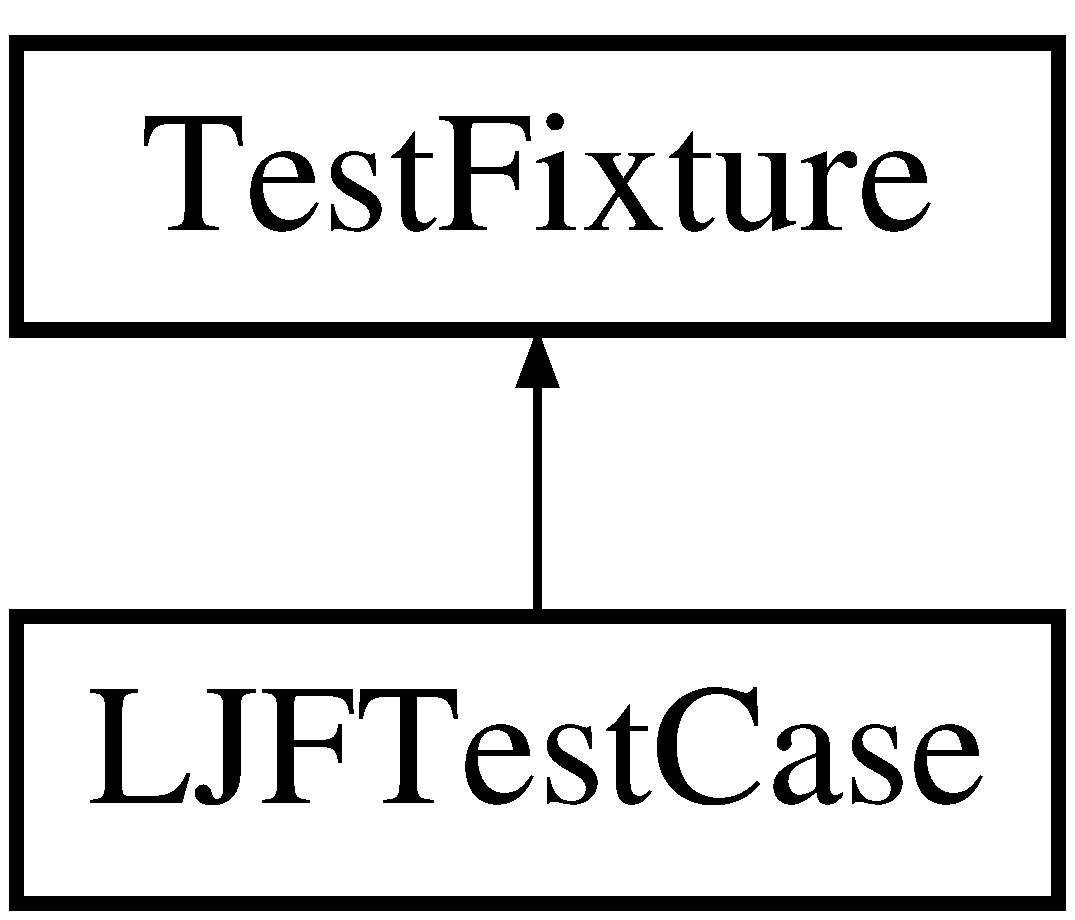
\includegraphics[height=2.000000cm]{class_l_j_f_test_case}
\end{center}
\end{figure}
\subsection*{Public Member Functions}
\begin{DoxyCompactItemize}
\item 
void \hyperlink{class_l_j_f_test_case_ab3b5deb3ab468b271d65041c3ba418eb}{set\+Up} ()
\item 
void \hyperlink{class_l_j_f_test_case_a47f0772df53a900d6870f970625f6d7a}{tear\+Down} ()
\item 
void \hyperlink{class_l_j_f_test_case_a541d3c9f1e4ecbd03e4f777edf4a9a13}{test\+\_\+pop\+\_\+task} ()
\item 
void \hyperlink{class_l_j_f_test_case_a381a8c163616c0752ce59ca44aff5849}{test\+\_\+push\+\_\+new\+\_\+task} ()
\item 
void \hyperlink{class_l_j_f_test_case_a81f6f3b146f1d10b687dc647d4398987}{test\+\_\+is\+\_\+statistic\+\_\+based} ()
\item 
void \hyperlink{class_l_j_f_test_case_aad808d4d522ec3ad9b1ab33abad16f24}{test\+\_\+get\+\_\+count} ()
\item 
void \hyperlink{class_l_j_f_test_case_a429f7b9280917c4ffd3cf898d7d804c1}{test\+\_\+get\+\_\+next\+\_\+task} ()
\end{DoxyCompactItemize}
\subsection*{Static Public Member Functions}
\begin{DoxyCompactItemize}
\item 
static Test $\ast$ \hyperlink{class_l_j_f_test_case_a1f51591cecf2427561abd7efda1f56ab}{suite} ()
\end{DoxyCompactItemize}


\subsection{Detailed Description}


Definition at line 24 of file L\+J\+F\+Test\+Case.\+h.



\subsection{Member Function Documentation}
\hypertarget{class_l_j_f_test_case_ab3b5deb3ab468b271d65041c3ba418eb}{}\index{L\+J\+F\+Test\+Case@{L\+J\+F\+Test\+Case}!set\+Up@{set\+Up}}
\index{set\+Up@{set\+Up}!L\+J\+F\+Test\+Case@{L\+J\+F\+Test\+Case}}
\subsubsection[{set\+Up}]{\setlength{\rightskip}{0pt plus 5cm}void L\+J\+F\+Test\+Case\+::set\+Up (
\begin{DoxyParamCaption}
{}
\end{DoxyParamCaption}
)}\label{class_l_j_f_test_case_ab3b5deb3ab468b271d65041c3ba418eb}


Definition at line 30 of file L\+J\+F\+Test\+Case.\+cpp.

\hypertarget{class_l_j_f_test_case_a1f51591cecf2427561abd7efda1f56ab}{}\index{L\+J\+F\+Test\+Case@{L\+J\+F\+Test\+Case}!suite@{suite}}
\index{suite@{suite}!L\+J\+F\+Test\+Case@{L\+J\+F\+Test\+Case}}
\subsubsection[{suite}]{\setlength{\rightskip}{0pt plus 5cm}Test $\ast$ L\+J\+F\+Test\+Case\+::suite (
\begin{DoxyParamCaption}
{}
\end{DoxyParamCaption}
)\hspace{0.3cm}{\ttfamily [static]}}\label{class_l_j_f_test_case_a1f51591cecf2427561abd7efda1f56ab}


Definition at line 19 of file L\+J\+F\+Test\+Case.\+cpp.

\hypertarget{class_l_j_f_test_case_a47f0772df53a900d6870f970625f6d7a}{}\index{L\+J\+F\+Test\+Case@{L\+J\+F\+Test\+Case}!tear\+Down@{tear\+Down}}
\index{tear\+Down@{tear\+Down}!L\+J\+F\+Test\+Case@{L\+J\+F\+Test\+Case}}
\subsubsection[{tear\+Down}]{\setlength{\rightskip}{0pt plus 5cm}void L\+J\+F\+Test\+Case\+::tear\+Down (
\begin{DoxyParamCaption}
{}
\end{DoxyParamCaption}
)}\label{class_l_j_f_test_case_a47f0772df53a900d6870f970625f6d7a}


Definition at line 34 of file L\+J\+F\+Test\+Case.\+cpp.

\hypertarget{class_l_j_f_test_case_aad808d4d522ec3ad9b1ab33abad16f24}{}\index{L\+J\+F\+Test\+Case@{L\+J\+F\+Test\+Case}!test\+\_\+get\+\_\+count@{test\+\_\+get\+\_\+count}}
\index{test\+\_\+get\+\_\+count@{test\+\_\+get\+\_\+count}!L\+J\+F\+Test\+Case@{L\+J\+F\+Test\+Case}}
\subsubsection[{test\+\_\+get\+\_\+count}]{\setlength{\rightskip}{0pt plus 5cm}void L\+J\+F\+Test\+Case\+::test\+\_\+get\+\_\+count (
\begin{DoxyParamCaption}
{}
\end{DoxyParamCaption}
)}\label{class_l_j_f_test_case_aad808d4d522ec3ad9b1ab33abad16f24}


Definition at line 42 of file L\+J\+F\+Test\+Case.\+cpp.

\hypertarget{class_l_j_f_test_case_a429f7b9280917c4ffd3cf898d7d804c1}{}\index{L\+J\+F\+Test\+Case@{L\+J\+F\+Test\+Case}!test\+\_\+get\+\_\+next\+\_\+task@{test\+\_\+get\+\_\+next\+\_\+task}}
\index{test\+\_\+get\+\_\+next\+\_\+task@{test\+\_\+get\+\_\+next\+\_\+task}!L\+J\+F\+Test\+Case@{L\+J\+F\+Test\+Case}}
\subsubsection[{test\+\_\+get\+\_\+next\+\_\+task}]{\setlength{\rightskip}{0pt plus 5cm}void L\+J\+F\+Test\+Case\+::test\+\_\+get\+\_\+next\+\_\+task (
\begin{DoxyParamCaption}
{}
\end{DoxyParamCaption}
)}\label{class_l_j_f_test_case_a429f7b9280917c4ffd3cf898d7d804c1}


Definition at line 79 of file L\+J\+F\+Test\+Case.\+cpp.

\hypertarget{class_l_j_f_test_case_a81f6f3b146f1d10b687dc647d4398987}{}\index{L\+J\+F\+Test\+Case@{L\+J\+F\+Test\+Case}!test\+\_\+is\+\_\+statistic\+\_\+based@{test\+\_\+is\+\_\+statistic\+\_\+based}}
\index{test\+\_\+is\+\_\+statistic\+\_\+based@{test\+\_\+is\+\_\+statistic\+\_\+based}!L\+J\+F\+Test\+Case@{L\+J\+F\+Test\+Case}}
\subsubsection[{test\+\_\+is\+\_\+statistic\+\_\+based}]{\setlength{\rightskip}{0pt plus 5cm}void L\+J\+F\+Test\+Case\+::test\+\_\+is\+\_\+statistic\+\_\+based (
\begin{DoxyParamCaption}
{}
\end{DoxyParamCaption}
)}\label{class_l_j_f_test_case_a81f6f3b146f1d10b687dc647d4398987}


Definition at line 38 of file L\+J\+F\+Test\+Case.\+cpp.

\hypertarget{class_l_j_f_test_case_a541d3c9f1e4ecbd03e4f777edf4a9a13}{}\index{L\+J\+F\+Test\+Case@{L\+J\+F\+Test\+Case}!test\+\_\+pop\+\_\+task@{test\+\_\+pop\+\_\+task}}
\index{test\+\_\+pop\+\_\+task@{test\+\_\+pop\+\_\+task}!L\+J\+F\+Test\+Case@{L\+J\+F\+Test\+Case}}
\subsubsection[{test\+\_\+pop\+\_\+task}]{\setlength{\rightskip}{0pt plus 5cm}void L\+J\+F\+Test\+Case\+::test\+\_\+pop\+\_\+task (
\begin{DoxyParamCaption}
{}
\end{DoxyParamCaption}
)}\label{class_l_j_f_test_case_a541d3c9f1e4ecbd03e4f777edf4a9a13}


Definition at line 53 of file L\+J\+F\+Test\+Case.\+cpp.

\hypertarget{class_l_j_f_test_case_a381a8c163616c0752ce59ca44aff5849}{}\index{L\+J\+F\+Test\+Case@{L\+J\+F\+Test\+Case}!test\+\_\+push\+\_\+new\+\_\+task@{test\+\_\+push\+\_\+new\+\_\+task}}
\index{test\+\_\+push\+\_\+new\+\_\+task@{test\+\_\+push\+\_\+new\+\_\+task}!L\+J\+F\+Test\+Case@{L\+J\+F\+Test\+Case}}
\subsubsection[{test\+\_\+push\+\_\+new\+\_\+task}]{\setlength{\rightskip}{0pt plus 5cm}void L\+J\+F\+Test\+Case\+::test\+\_\+push\+\_\+new\+\_\+task (
\begin{DoxyParamCaption}
{}
\end{DoxyParamCaption}
)}\label{class_l_j_f_test_case_a381a8c163616c0752ce59ca44aff5849}


Definition at line 68 of file L\+J\+F\+Test\+Case.\+cpp.



The documentation for this class was generated from the following files\+:\begin{DoxyCompactItemize}
\item 
test/scheduler/\hyperlink{_l_j_f_test_case_8h}{L\+J\+F\+Test\+Case.\+h}\item 
test/scheduler/\hyperlink{_l_j_f_test_case_8cpp}{L\+J\+F\+Test\+Case.\+cpp}\end{DoxyCompactItemize}

\hypertarget{classel_1_1_log_builder}{}\section{el\+:\+:Log\+Builder Class Reference}
\label{classel_1_1_log_builder}\index{el\+::\+Log\+Builder@{el\+::\+Log\+Builder}}


{\ttfamily \#include $<$easylogging++.\+h$>$}

Inheritance diagram for el\+:\+:Log\+Builder\+:\begin{figure}[H]
\begin{center}
\leavevmode
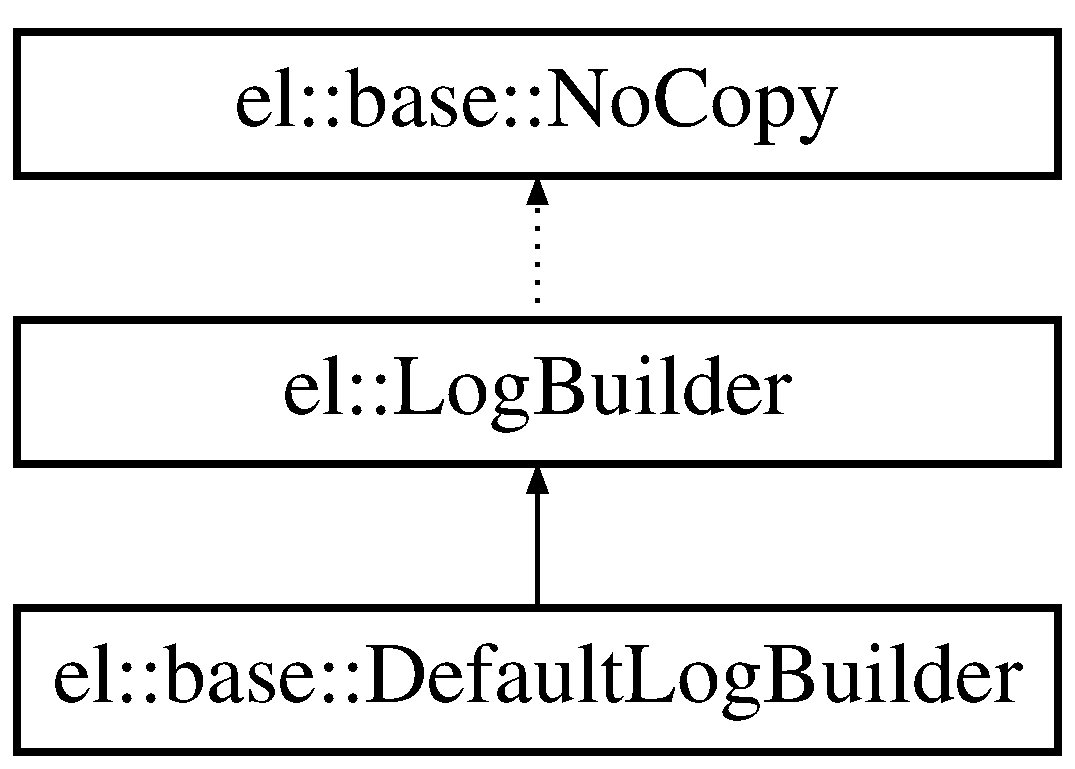
\includegraphics[height=3.000000cm]{classel_1_1_log_builder}
\end{center}
\end{figure}
\subsection*{Public Member Functions}
\begin{DoxyCompactItemize}
\item 
virtual \hyperlink{classel_1_1_log_builder_ae45008e1c004367ef611b22662e7ed72}{$\sim$\+Log\+Builder} (void)
\item 
virtual \hyperlink{namespaceel_1_1base_1_1type_a67e406cd213c231f1d135b5a4eda64b5}{base\+::type\+::string\+\_\+t} \hyperlink{classel_1_1_log_builder_a633b373a3bb9d3e17bdd664aeba4dbc8}{build} (const \hyperlink{classel_1_1_log_message}{Log\+Message} $\ast$log\+Message, bool append\+New\+Line) const =0
\item 
void \hyperlink{classel_1_1_log_builder_a229244f323f25bdbd7725f8bbf983a17}{convert\+To\+Colored\+Output} (\hyperlink{namespaceel_1_1base_1_1type_a67e406cd213c231f1d135b5a4eda64b5}{base\+::type\+::string\+\_\+t} $\ast$log\+Line, \hyperlink{namespaceel_ab0ac6091262344c52dd2d3ad099e8e36}{Level} level)
\end{DoxyCompactItemize}
\subsection*{Friends}
\begin{DoxyCompactItemize}
\item 
class \hyperlink{classel_1_1_log_builder_a42b1de96d584ae4fecbfc2b9aff95052}{el\+::base\+::\+Default\+Log\+Dispatch\+Callback}
\end{DoxyCompactItemize}


\subsection{Detailed Description}


Definition at line 3355 of file easylogging++.\+h.



\subsection{Constructor \& Destructor Documentation}
\hypertarget{classel_1_1_log_builder_ae45008e1c004367ef611b22662e7ed72}{}\index{el\+::\+Log\+Builder@{el\+::\+Log\+Builder}!````~Log\+Builder@{$\sim$\+Log\+Builder}}
\index{````~Log\+Builder@{$\sim$\+Log\+Builder}!el\+::\+Log\+Builder@{el\+::\+Log\+Builder}}
\subsubsection[{$\sim$\+Log\+Builder}]{\setlength{\rightskip}{0pt plus 5cm}virtual el\+::\+Log\+Builder\+::$\sim$\+Log\+Builder (
\begin{DoxyParamCaption}
\item[{void}]{}
\end{DoxyParamCaption}
)\hspace{0.3cm}{\ttfamily [inline]}, {\ttfamily [virtual]}}\label{classel_1_1_log_builder_ae45008e1c004367ef611b22662e7ed72}


Definition at line 3357 of file easylogging++.\+h.



\subsection{Member Function Documentation}
\hypertarget{classel_1_1_log_builder_a633b373a3bb9d3e17bdd664aeba4dbc8}{}\index{el\+::\+Log\+Builder@{el\+::\+Log\+Builder}!build@{build}}
\index{build@{build}!el\+::\+Log\+Builder@{el\+::\+Log\+Builder}}
\subsubsection[{build}]{\setlength{\rightskip}{0pt plus 5cm}virtual {\bf base\+::type\+::string\+\_\+t} el\+::\+Log\+Builder\+::build (
\begin{DoxyParamCaption}
\item[{const {\bf Log\+Message} $\ast$}]{log\+Message, }
\item[{bool}]{append\+New\+Line}
\end{DoxyParamCaption}
) const\hspace{0.3cm}{\ttfamily [pure virtual]}}\label{classel_1_1_log_builder_a633b373a3bb9d3e17bdd664aeba4dbc8}


Implemented in \hyperlink{classel_1_1base_1_1_default_log_builder_aa8d2f42068115d899ed81de1b0ed360e}{el\+::base\+::\+Default\+Log\+Builder}.

\hypertarget{classel_1_1_log_builder_a229244f323f25bdbd7725f8bbf983a17}{}\index{el\+::\+Log\+Builder@{el\+::\+Log\+Builder}!convert\+To\+Colored\+Output@{convert\+To\+Colored\+Output}}
\index{convert\+To\+Colored\+Output@{convert\+To\+Colored\+Output}!el\+::\+Log\+Builder@{el\+::\+Log\+Builder}}
\subsubsection[{convert\+To\+Colored\+Output}]{\setlength{\rightskip}{0pt plus 5cm}void el\+::\+Log\+Builder\+::convert\+To\+Colored\+Output (
\begin{DoxyParamCaption}
\item[{{\bf base\+::type\+::string\+\_\+t} $\ast$}]{log\+Line, }
\item[{{\bf Level}}]{level}
\end{DoxyParamCaption}
)\hspace{0.3cm}{\ttfamily [inline]}}\label{classel_1_1_log_builder_a229244f323f25bdbd7725f8bbf983a17}


Definition at line 3359 of file easylogging++.\+h.



\subsection{Friends And Related Function Documentation}
\hypertarget{classel_1_1_log_builder_a42b1de96d584ae4fecbfc2b9aff95052}{}\index{el\+::\+Log\+Builder@{el\+::\+Log\+Builder}!el\+::base\+::\+Default\+Log\+Dispatch\+Callback@{el\+::base\+::\+Default\+Log\+Dispatch\+Callback}}
\index{el\+::base\+::\+Default\+Log\+Dispatch\+Callback@{el\+::base\+::\+Default\+Log\+Dispatch\+Callback}!el\+::\+Log\+Builder@{el\+::\+Log\+Builder}}
\subsubsection[{el\+::base\+::\+Default\+Log\+Dispatch\+Callback}]{\setlength{\rightskip}{0pt plus 5cm}friend class {\bf el\+::base\+::\+Default\+Log\+Dispatch\+Callback}\hspace{0.3cm}{\ttfamily [friend]}}\label{classel_1_1_log_builder_a42b1de96d584ae4fecbfc2b9aff95052}


Definition at line 3368 of file easylogging++.\+h.



The documentation for this class was generated from the following file\+:\begin{DoxyCompactItemize}
\item 
lib/\hyperlink{easylogging_09_09_8h}{easylogging++.\+h}\end{DoxyCompactItemize}

\hypertarget{classel_1_1_log_dispatch_callback}{}\section{el\+:\+:Log\+Dispatch\+Callback Class Reference}
\label{classel_1_1_log_dispatch_callback}\index{el\+::\+Log\+Dispatch\+Callback@{el\+::\+Log\+Dispatch\+Callback}}


{\ttfamily \#include $<$easylogging++.\+h$>$}

Inheritance diagram for el\+:\+:Log\+Dispatch\+Callback\+:\begin{figure}[H]
\begin{center}
\leavevmode
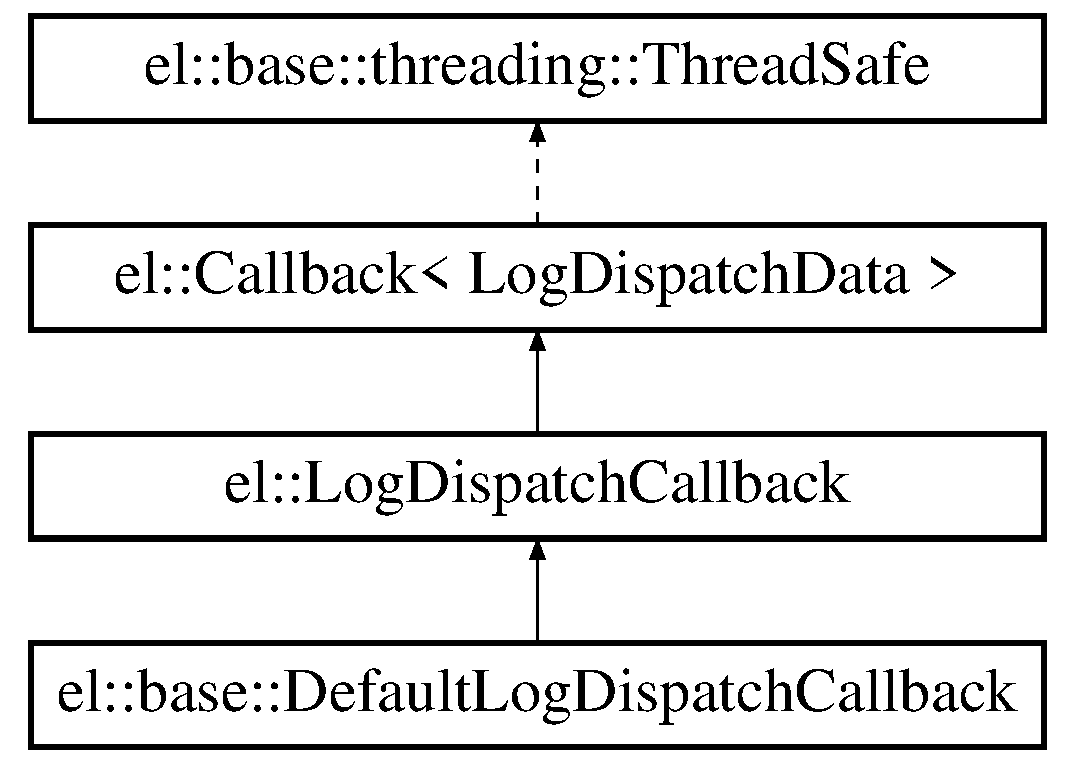
\includegraphics[height=4.000000cm]{classel_1_1_log_dispatch_callback}
\end{center}
\end{figure}
\subsection*{Friends}
\begin{DoxyCompactItemize}
\item 
class \hyperlink{classel_1_1_log_dispatch_callback_a84d22f9ad5b796e49ff5f15a8c32773d}{base\+::\+Log\+Dispatcher}
\end{DoxyCompactItemize}
\subsection*{Additional Inherited Members}


\subsection{Detailed Description}


Definition at line 3347 of file easylogging++.\+h.



\subsection{Friends And Related Function Documentation}
\hypertarget{classel_1_1_log_dispatch_callback_a84d22f9ad5b796e49ff5f15a8c32773d}{}\index{el\+::\+Log\+Dispatch\+Callback@{el\+::\+Log\+Dispatch\+Callback}!base\+::\+Log\+Dispatcher@{base\+::\+Log\+Dispatcher}}
\index{base\+::\+Log\+Dispatcher@{base\+::\+Log\+Dispatcher}!el\+::\+Log\+Dispatch\+Callback@{el\+::\+Log\+Dispatch\+Callback}}
\subsubsection[{base\+::\+Log\+Dispatcher}]{\setlength{\rightskip}{0pt plus 5cm}friend class {\bf base\+::\+Log\+Dispatcher}\hspace{0.3cm}{\ttfamily [friend]}}\label{classel_1_1_log_dispatch_callback_a84d22f9ad5b796e49ff5f15a8c32773d}


Definition at line 3349 of file easylogging++.\+h.



The documentation for this class was generated from the following file\+:\begin{DoxyCompactItemize}
\item 
lib/\hyperlink{easylogging_09_09_8h}{easylogging++.\+h}\end{DoxyCompactItemize}

\hypertarget{classel_1_1_log_dispatch_data}{}\section{el\+:\+:Log\+Dispatch\+Data Class Reference}
\label{classel_1_1_log_dispatch_data}\index{el\+::\+Log\+Dispatch\+Data@{el\+::\+Log\+Dispatch\+Data}}


{\ttfamily \#include $<$easylogging++.\+h$>$}

\subsection*{Public Member Functions}
\begin{DoxyCompactItemize}
\item 
\hyperlink{classel_1_1_log_dispatch_data_a851cab4e58658e3dc8267427fd1e3572}{Log\+Dispatch\+Data} ()
\item 
const \hyperlink{classel_1_1_log_message}{Log\+Message} $\ast$ \hyperlink{classel_1_1_log_dispatch_data_ad52d4ddc330b6260bf10e9879a653829}{log\+Message} (void) const 
\item 
\hyperlink{namespaceel_1_1base_a3aa2563d38e47388ba242a1694fc2839}{base\+::\+Dispatch\+Action} \hyperlink{classel_1_1_log_dispatch_data_aee0808c660aa39b34ee69850a2c74c09}{dispatch\+Action} (void) const 
\end{DoxyCompactItemize}
\subsection*{Friends}
\begin{DoxyCompactItemize}
\item 
class \hyperlink{classel_1_1_log_dispatch_data_a84d22f9ad5b796e49ff5f15a8c32773d}{base\+::\+Log\+Dispatcher}
\end{DoxyCompactItemize}


\subsection{Detailed Description}


Definition at line 3334 of file easylogging++.\+h.



\subsection{Constructor \& Destructor Documentation}
\hypertarget{classel_1_1_log_dispatch_data_a851cab4e58658e3dc8267427fd1e3572}{}\index{el\+::\+Log\+Dispatch\+Data@{el\+::\+Log\+Dispatch\+Data}!Log\+Dispatch\+Data@{Log\+Dispatch\+Data}}
\index{Log\+Dispatch\+Data@{Log\+Dispatch\+Data}!el\+::\+Log\+Dispatch\+Data@{el\+::\+Log\+Dispatch\+Data}}
\subsubsection[{Log\+Dispatch\+Data}]{\setlength{\rightskip}{0pt plus 5cm}el\+::\+Log\+Dispatch\+Data\+::\+Log\+Dispatch\+Data (
\begin{DoxyParamCaption}
{}
\end{DoxyParamCaption}
)\hspace{0.3cm}{\ttfamily [inline]}}\label{classel_1_1_log_dispatch_data_a851cab4e58658e3dc8267427fd1e3572}


Definition at line 3336 of file easylogging++.\+h.



\subsection{Member Function Documentation}
\hypertarget{classel_1_1_log_dispatch_data_aee0808c660aa39b34ee69850a2c74c09}{}\index{el\+::\+Log\+Dispatch\+Data@{el\+::\+Log\+Dispatch\+Data}!dispatch\+Action@{dispatch\+Action}}
\index{dispatch\+Action@{dispatch\+Action}!el\+::\+Log\+Dispatch\+Data@{el\+::\+Log\+Dispatch\+Data}}
\subsubsection[{dispatch\+Action}]{\setlength{\rightskip}{0pt plus 5cm}{\bf base\+::\+Dispatch\+Action} el\+::\+Log\+Dispatch\+Data\+::dispatch\+Action (
\begin{DoxyParamCaption}
\item[{void}]{}
\end{DoxyParamCaption}
) const\hspace{0.3cm}{\ttfamily [inline]}}\label{classel_1_1_log_dispatch_data_aee0808c660aa39b34ee69850a2c74c09}


Definition at line 3338 of file easylogging++.\+h.

\hypertarget{classel_1_1_log_dispatch_data_ad52d4ddc330b6260bf10e9879a653829}{}\index{el\+::\+Log\+Dispatch\+Data@{el\+::\+Log\+Dispatch\+Data}!log\+Message@{log\+Message}}
\index{log\+Message@{log\+Message}!el\+::\+Log\+Dispatch\+Data@{el\+::\+Log\+Dispatch\+Data}}
\subsubsection[{log\+Message}]{\setlength{\rightskip}{0pt plus 5cm}const {\bf Log\+Message}$\ast$ el\+::\+Log\+Dispatch\+Data\+::log\+Message (
\begin{DoxyParamCaption}
\item[{void}]{}
\end{DoxyParamCaption}
) const\hspace{0.3cm}{\ttfamily [inline]}}\label{classel_1_1_log_dispatch_data_ad52d4ddc330b6260bf10e9879a653829}


Definition at line 3337 of file easylogging++.\+h.



\subsection{Friends And Related Function Documentation}
\hypertarget{classel_1_1_log_dispatch_data_a84d22f9ad5b796e49ff5f15a8c32773d}{}\index{el\+::\+Log\+Dispatch\+Data@{el\+::\+Log\+Dispatch\+Data}!base\+::\+Log\+Dispatcher@{base\+::\+Log\+Dispatcher}}
\index{base\+::\+Log\+Dispatcher@{base\+::\+Log\+Dispatcher}!el\+::\+Log\+Dispatch\+Data@{el\+::\+Log\+Dispatch\+Data}}
\subsubsection[{base\+::\+Log\+Dispatcher}]{\setlength{\rightskip}{0pt plus 5cm}friend class {\bf base\+::\+Log\+Dispatcher}\hspace{0.3cm}{\ttfamily [friend]}}\label{classel_1_1_log_dispatch_data_a84d22f9ad5b796e49ff5f15a8c32773d}


Definition at line 3342 of file easylogging++.\+h.



The documentation for this class was generated from the following file\+:\begin{DoxyCompactItemize}
\item 
lib/\hyperlink{easylogging_09_09_8h}{easylogging++.\+h}\end{DoxyCompactItemize}

\hypertarget{classel_1_1base_1_1_log_dispatcher}{}\section{el\+:\+:base\+:\+:Log\+Dispatcher Class Reference}
\label{classel_1_1base_1_1_log_dispatcher}\index{el\+::base\+::\+Log\+Dispatcher@{el\+::base\+::\+Log\+Dispatcher}}


Dispatches log messages.  




{\ttfamily \#include $<$easylogging++.\+h$>$}

Inheritance diagram for el\+:\+:base\+:\+:Log\+Dispatcher\+:\begin{figure}[H]
\begin{center}
\leavevmode
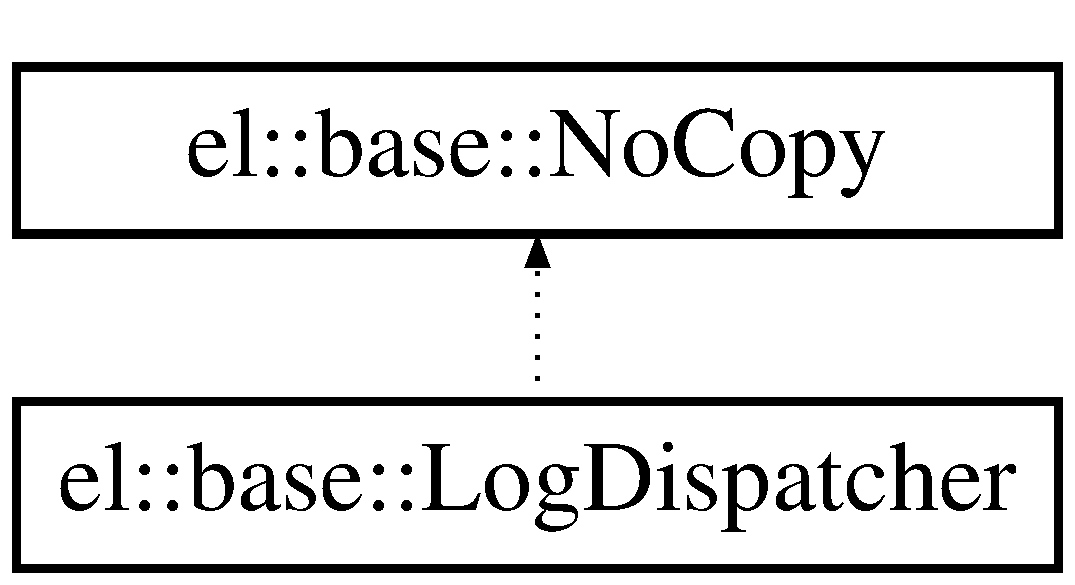
\includegraphics[height=2.000000cm]{classel_1_1base_1_1_log_dispatcher}
\end{center}
\end{figure}
\subsection*{Public Member Functions}
\begin{DoxyCompactItemize}
\item 
\hyperlink{classel_1_1base_1_1_log_dispatcher_aef59d9895c348f0b3ad5a776276f1c22}{Log\+Dispatcher} (bool proceed, \hyperlink{classel_1_1_log_message}{Log\+Message} \&\&log\+Message, \hyperlink{namespaceel_1_1base_a3aa2563d38e47388ba242a1694fc2839}{base\+::\+Dispatch\+Action} dispatch\+Action)
\item 
void \hyperlink{classel_1_1base_1_1_log_dispatcher_a88d4a644364bb454136c85338f05da7a}{dispatch} (void)
\end{DoxyCompactItemize}


\subsection{Detailed Description}
Dispatches log messages. 

Definition at line 4450 of file easylogging++.\+h.



\subsection{Constructor \& Destructor Documentation}
\hypertarget{classel_1_1base_1_1_log_dispatcher_aef59d9895c348f0b3ad5a776276f1c22}{}\index{el\+::base\+::\+Log\+Dispatcher@{el\+::base\+::\+Log\+Dispatcher}!Log\+Dispatcher@{Log\+Dispatcher}}
\index{Log\+Dispatcher@{Log\+Dispatcher}!el\+::base\+::\+Log\+Dispatcher@{el\+::base\+::\+Log\+Dispatcher}}
\subsubsection[{Log\+Dispatcher}]{\setlength{\rightskip}{0pt plus 5cm}el\+::base\+::\+Log\+Dispatcher\+::\+Log\+Dispatcher (
\begin{DoxyParamCaption}
\item[{bool}]{proceed, }
\item[{{\bf Log\+Message} \&\&}]{log\+Message, }
\item[{{\bf base\+::\+Dispatch\+Action}}]{dispatch\+Action}
\end{DoxyParamCaption}
)\hspace{0.3cm}{\ttfamily [inline]}}\label{classel_1_1base_1_1_log_dispatcher_aef59d9895c348f0b3ad5a776276f1c22}


Definition at line 4452 of file easylogging++.\+h.



\subsection{Member Function Documentation}
\hypertarget{classel_1_1base_1_1_log_dispatcher_a88d4a644364bb454136c85338f05da7a}{}\index{el\+::base\+::\+Log\+Dispatcher@{el\+::base\+::\+Log\+Dispatcher}!dispatch@{dispatch}}
\index{dispatch@{dispatch}!el\+::base\+::\+Log\+Dispatcher@{el\+::base\+::\+Log\+Dispatcher}}
\subsubsection[{dispatch}]{\setlength{\rightskip}{0pt plus 5cm}void el\+::base\+::\+Log\+Dispatcher\+::dispatch (
\begin{DoxyParamCaption}
\item[{void}]{}
\end{DoxyParamCaption}
)\hspace{0.3cm}{\ttfamily [inline]}}\label{classel_1_1base_1_1_log_dispatcher_a88d4a644364bb454136c85338f05da7a}


Definition at line 4458 of file easylogging++.\+h.



The documentation for this class was generated from the following file\+:\begin{DoxyCompactItemize}
\item 
lib/\hyperlink{easylogging_09_09_8h}{easylogging++.\+h}\end{DoxyCompactItemize}

\hypertarget{classel_1_1base_1_1_log_format}{}\section{el\+:\+:base\+:\+:Log\+Format Class Reference}
\label{classel_1_1base_1_1_log_format}\index{el\+::base\+::\+Log\+Format@{el\+::base\+::\+Log\+Format}}


Represents log format containing flags and date format. This is used internally to start initial log.  




{\ttfamily \#include $<$easylogging++.\+h$>$}

Inheritance diagram for el\+:\+:base\+:\+:Log\+Format\+:\begin{figure}[H]
\begin{center}
\leavevmode
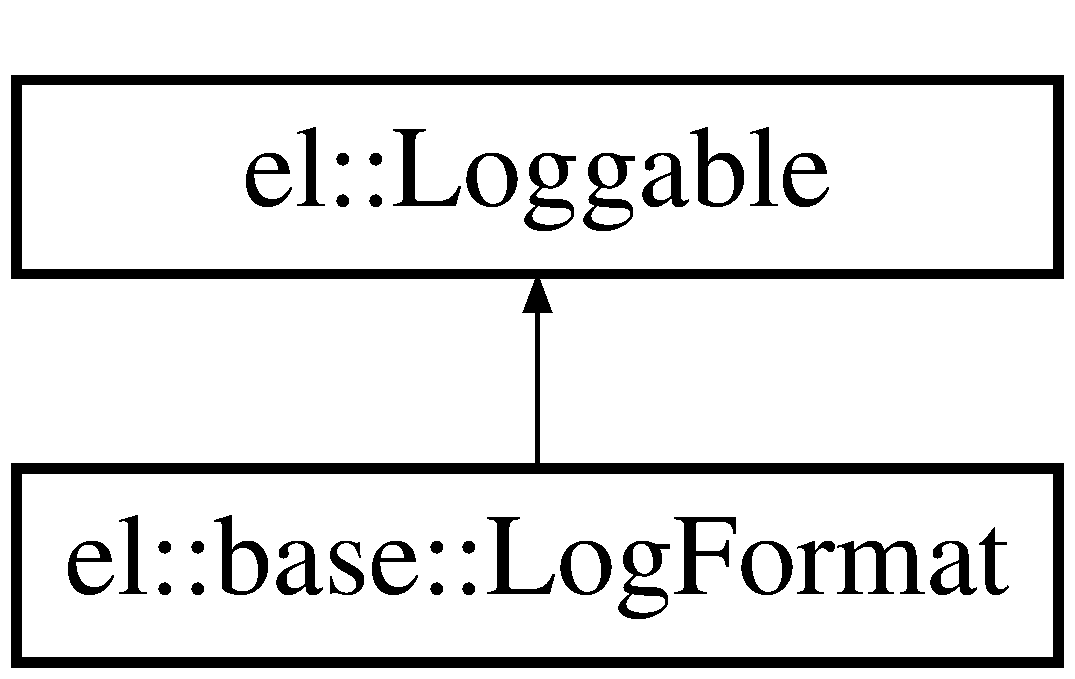
\includegraphics[height=2.000000cm]{classel_1_1base_1_1_log_format}
\end{center}
\end{figure}
\subsection*{Public Member Functions}
\begin{DoxyCompactItemize}
\item 
\hyperlink{classel_1_1base_1_1_log_format_a15469c6f25aa4a4770b1d2aeaabba145}{Log\+Format} (void)
\item 
\hyperlink{classel_1_1base_1_1_log_format_a746a49231f1b046803dd2144ae2a2c76}{Log\+Format} (\hyperlink{namespaceel_ab0ac6091262344c52dd2d3ad099e8e36}{Level} \hyperlink{classel_1_1base_1_1_log_format_a6c5d17ad378ccb6e53beb2d48143fecb}{level}, const \hyperlink{namespaceel_1_1base_1_1type_a67e406cd213c231f1d135b5a4eda64b5}{base\+::type\+::string\+\_\+t} \&\hyperlink{classel_1_1base_1_1_log_format_ac19602b3153daa9a76b56d3f4ff3beaa}{format})
\item 
\hyperlink{classel_1_1base_1_1_log_format_a8cc88ab095024bcfb90dd3ad7208f2ef}{Log\+Format} (const \hyperlink{classel_1_1base_1_1_log_format}{Log\+Format} \&log\+Format)
\item 
\hyperlink{classel_1_1base_1_1_log_format_a697d52d55c6b6c6b8e6d5ceb37d66c19}{Log\+Format} (\hyperlink{classel_1_1base_1_1_log_format}{Log\+Format} \&\&log\+Format)
\item 
\hyperlink{classel_1_1base_1_1_log_format}{Log\+Format} \& \hyperlink{classel_1_1base_1_1_log_format_a3c81e5976c3f3a8cb428eeeb3f188ac2}{operator=} (const \hyperlink{classel_1_1base_1_1_log_format}{Log\+Format} \&log\+Format)
\item 
virtual \hyperlink{classel_1_1base_1_1_log_format_a09d5b42b49f00fb37edafef1102daf0c}{$\sim$\+Log\+Format} (void)
\item 
bool \hyperlink{classel_1_1base_1_1_log_format_a31e85c6f74da6fe36d156a89a6c7fb91}{operator==} (const \hyperlink{classel_1_1base_1_1_log_format}{Log\+Format} \&other)
\item 
void \hyperlink{classel_1_1base_1_1_log_format_ab7c1b15cfdad24cfbc6dbced8b9d66eb}{parse\+From\+Format} (const \hyperlink{namespaceel_1_1base_1_1type_a67e406cd213c231f1d135b5a4eda64b5}{base\+::type\+::string\+\_\+t} \&\hyperlink{classel_1_1base_1_1_log_format_a9ca6ecd5b9342653493670d5a4e230cd}{user\+Format})
\begin{DoxyCompactList}\small\item\em Updates format to be used while logging. \end{DoxyCompactList}\item 
\hyperlink{namespaceel_ab0ac6091262344c52dd2d3ad099e8e36}{Level} \hyperlink{classel_1_1base_1_1_log_format_a6c5d17ad378ccb6e53beb2d48143fecb}{level} (void) const 
\item 
const \hyperlink{namespaceel_1_1base_1_1type_a67e406cd213c231f1d135b5a4eda64b5}{base\+::type\+::string\+\_\+t} \& \hyperlink{classel_1_1base_1_1_log_format_a9ca6ecd5b9342653493670d5a4e230cd}{user\+Format} (void) const 
\item 
const \hyperlink{namespaceel_1_1base_1_1type_a67e406cd213c231f1d135b5a4eda64b5}{base\+::type\+::string\+\_\+t} \& \hyperlink{classel_1_1base_1_1_log_format_ac19602b3153daa9a76b56d3f4ff3beaa}{format} (void) const 
\item 
const std\+::string \& \hyperlink{classel_1_1base_1_1_log_format_aa06b2643592f8a441d93cde673640262}{date\+Time\+Format} (void) const 
\item 
\hyperlink{namespaceel_1_1base_1_1type_afb892a99b7545bf6e45c1e1d84af2ec9}{base\+::type\+::\+Enum\+Type} \hyperlink{classel_1_1base_1_1_log_format_a3ecf5f8df9b9e090784e19ad76046c49}{flags} (void) const 
\item 
bool \hyperlink{classel_1_1base_1_1_log_format_ae3634f9d90f7339d99eec8512b46c734}{has\+Flag} (\hyperlink{namespaceel_1_1base_a28939c5a884e67fcf12259f4b8848e00}{base\+::\+Format\+Flags} flag) const 
\item 
virtual void \hyperlink{classel_1_1base_1_1_log_format_a0cae595d1a367538243feb1be1555d2e}{log} (\hyperlink{namespaceel_1_1base_1_1type_a74ea109bf34d1c44926837fb0830f445}{el\+::base\+::type\+::ostream\+\_\+t} \&os) const 
\end{DoxyCompactItemize}
\subsection*{Protected Member Functions}
\begin{DoxyCompactItemize}
\item 
virtual void \hyperlink{classel_1_1base_1_1_log_format_a3146651eadd6b1164bde74e5b273ec94}{update\+Date\+Format} (std\+::size\+\_\+t index, \hyperlink{namespaceel_1_1base_1_1type_a67e406cd213c231f1d135b5a4eda64b5}{base\+::type\+::string\+\_\+t} \&curr\+Format) \hyperlink{easylogging_09_09_8h_a2f812449f8d3355cf5b03ceb2ee5021b}{E\+L\+P\+P\+\_\+\+F\+I\+N\+A\+L}
\begin{DoxyCompactList}\small\item\em Updates date time format if available in curr\+Format. \end{DoxyCompactList}\item 
virtual void \hyperlink{classel_1_1base_1_1_log_format_afee2335cce2b627dfd7f918d5a2b85f3}{update\+Format\+Spec} (void) \hyperlink{easylogging_09_09_8h_a2f812449f8d3355cf5b03ceb2ee5021b}{E\+L\+P\+P\+\_\+\+F\+I\+N\+A\+L}
\begin{DoxyCompactList}\small\item\em Updates level from format. This is so that we dont have to do it at log-\/writing-\/time. It uses m\+\_\+format and m\+\_\+level. \end{DoxyCompactList}\item 
void \hyperlink{classel_1_1base_1_1_log_format_ae55910f533a6eb3b41eb75b131e522bf}{add\+Flag} (\hyperlink{namespaceel_1_1base_a28939c5a884e67fcf12259f4b8848e00}{base\+::\+Format\+Flags} flag)
\end{DoxyCompactItemize}
\subsection*{Friends}
\begin{DoxyCompactItemize}
\item 
class \hyperlink{classel_1_1base_1_1_log_format_aa78553f3fecc0d9551408dfd7aa7f737}{el\+::\+Logger}
\end{DoxyCompactItemize}


\subsection{Detailed Description}
Represents log format containing flags and date format. This is used internally to start initial log. 

Definition at line 2108 of file easylogging++.\+h.



\subsection{Constructor \& Destructor Documentation}
\hypertarget{classel_1_1base_1_1_log_format_a15469c6f25aa4a4770b1d2aeaabba145}{}\index{el\+::base\+::\+Log\+Format@{el\+::base\+::\+Log\+Format}!Log\+Format@{Log\+Format}}
\index{Log\+Format@{Log\+Format}!el\+::base\+::\+Log\+Format@{el\+::base\+::\+Log\+Format}}
\subsubsection[{Log\+Format}]{\setlength{\rightskip}{0pt plus 5cm}el\+::base\+::\+Log\+Format\+::\+Log\+Format (
\begin{DoxyParamCaption}
\item[{void}]{}
\end{DoxyParamCaption}
)\hspace{0.3cm}{\ttfamily [inline]}}\label{classel_1_1base_1_1_log_format_a15469c6f25aa4a4770b1d2aeaabba145}


Definition at line 2110 of file easylogging++.\+h.

\hypertarget{classel_1_1base_1_1_log_format_a746a49231f1b046803dd2144ae2a2c76}{}\index{el\+::base\+::\+Log\+Format@{el\+::base\+::\+Log\+Format}!Log\+Format@{Log\+Format}}
\index{Log\+Format@{Log\+Format}!el\+::base\+::\+Log\+Format@{el\+::base\+::\+Log\+Format}}
\subsubsection[{Log\+Format}]{\setlength{\rightskip}{0pt plus 5cm}el\+::base\+::\+Log\+Format\+::\+Log\+Format (
\begin{DoxyParamCaption}
\item[{{\bf Level}}]{level, }
\item[{const {\bf base\+::type\+::string\+\_\+t} \&}]{format}
\end{DoxyParamCaption}
)\hspace{0.3cm}{\ttfamily [inline]}}\label{classel_1_1base_1_1_log_format_a746a49231f1b046803dd2144ae2a2c76}


Definition at line 2118 of file easylogging++.\+h.

\hypertarget{classel_1_1base_1_1_log_format_a8cc88ab095024bcfb90dd3ad7208f2ef}{}\index{el\+::base\+::\+Log\+Format@{el\+::base\+::\+Log\+Format}!Log\+Format@{Log\+Format}}
\index{Log\+Format@{Log\+Format}!el\+::base\+::\+Log\+Format@{el\+::base\+::\+Log\+Format}}
\subsubsection[{Log\+Format}]{\setlength{\rightskip}{0pt plus 5cm}el\+::base\+::\+Log\+Format\+::\+Log\+Format (
\begin{DoxyParamCaption}
\item[{const {\bf Log\+Format} \&}]{log\+Format}
\end{DoxyParamCaption}
)\hspace{0.3cm}{\ttfamily [inline]}}\label{classel_1_1base_1_1_log_format_a8cc88ab095024bcfb90dd3ad7208f2ef}


Definition at line 2123 of file easylogging++.\+h.

\hypertarget{classel_1_1base_1_1_log_format_a697d52d55c6b6c6b8e6d5ceb37d66c19}{}\index{el\+::base\+::\+Log\+Format@{el\+::base\+::\+Log\+Format}!Log\+Format@{Log\+Format}}
\index{Log\+Format@{Log\+Format}!el\+::base\+::\+Log\+Format@{el\+::base\+::\+Log\+Format}}
\subsubsection[{Log\+Format}]{\setlength{\rightskip}{0pt plus 5cm}el\+::base\+::\+Log\+Format\+::\+Log\+Format (
\begin{DoxyParamCaption}
\item[{{\bf Log\+Format} \&\&}]{log\+Format}
\end{DoxyParamCaption}
)\hspace{0.3cm}{\ttfamily [inline]}}\label{classel_1_1base_1_1_log_format_a697d52d55c6b6c6b8e6d5ceb37d66c19}


Definition at line 2131 of file easylogging++.\+h.

\hypertarget{classel_1_1base_1_1_log_format_a09d5b42b49f00fb37edafef1102daf0c}{}\index{el\+::base\+::\+Log\+Format@{el\+::base\+::\+Log\+Format}!````~Log\+Format@{$\sim$\+Log\+Format}}
\index{````~Log\+Format@{$\sim$\+Log\+Format}!el\+::base\+::\+Log\+Format@{el\+::base\+::\+Log\+Format}}
\subsubsection[{$\sim$\+Log\+Format}]{\setlength{\rightskip}{0pt plus 5cm}virtual el\+::base\+::\+Log\+Format\+::$\sim$\+Log\+Format (
\begin{DoxyParamCaption}
\item[{void}]{}
\end{DoxyParamCaption}
)\hspace{0.3cm}{\ttfamily [inline]}, {\ttfamily [virtual]}}\label{classel_1_1base_1_1_log_format_a09d5b42b49f00fb37edafef1102daf0c}


Definition at line 2147 of file easylogging++.\+h.



\subsection{Member Function Documentation}
\hypertarget{classel_1_1base_1_1_log_format_ae55910f533a6eb3b41eb75b131e522bf}{}\index{el\+::base\+::\+Log\+Format@{el\+::base\+::\+Log\+Format}!add\+Flag@{add\+Flag}}
\index{add\+Flag@{add\+Flag}!el\+::base\+::\+Log\+Format@{el\+::base\+::\+Log\+Format}}
\subsubsection[{add\+Flag}]{\setlength{\rightskip}{0pt plus 5cm}void el\+::base\+::\+Log\+Format\+::add\+Flag (
\begin{DoxyParamCaption}
\item[{{\bf base\+::\+Format\+Flags}}]{flag}
\end{DoxyParamCaption}
)\hspace{0.3cm}{\ttfamily [inline]}, {\ttfamily [protected]}}\label{classel_1_1base_1_1_log_format_ae55910f533a6eb3b41eb75b131e522bf}


Definition at line 2317 of file easylogging++.\+h.

\hypertarget{classel_1_1base_1_1_log_format_aa06b2643592f8a441d93cde673640262}{}\index{el\+::base\+::\+Log\+Format@{el\+::base\+::\+Log\+Format}!date\+Time\+Format@{date\+Time\+Format}}
\index{date\+Time\+Format@{date\+Time\+Format}!el\+::base\+::\+Log\+Format@{el\+::base\+::\+Log\+Format}}
\subsubsection[{date\+Time\+Format}]{\setlength{\rightskip}{0pt plus 5cm}const std\+::string\& el\+::base\+::\+Log\+Format\+::date\+Time\+Format (
\begin{DoxyParamCaption}
\item[{void}]{}
\end{DoxyParamCaption}
) const\hspace{0.3cm}{\ttfamily [inline]}}\label{classel_1_1base_1_1_log_format_aa06b2643592f8a441d93cde673640262}


Definition at line 2219 of file easylogging++.\+h.

\hypertarget{classel_1_1base_1_1_log_format_a3ecf5f8df9b9e090784e19ad76046c49}{}\index{el\+::base\+::\+Log\+Format@{el\+::base\+::\+Log\+Format}!flags@{flags}}
\index{flags@{flags}!el\+::base\+::\+Log\+Format@{el\+::base\+::\+Log\+Format}}
\subsubsection[{flags}]{\setlength{\rightskip}{0pt plus 5cm}{\bf base\+::type\+::\+Enum\+Type} el\+::base\+::\+Log\+Format\+::flags (
\begin{DoxyParamCaption}
\item[{void}]{}
\end{DoxyParamCaption}
) const\hspace{0.3cm}{\ttfamily [inline]}}\label{classel_1_1base_1_1_log_format_a3ecf5f8df9b9e090784e19ad76046c49}


Definition at line 2223 of file easylogging++.\+h.

\hypertarget{classel_1_1base_1_1_log_format_ac19602b3153daa9a76b56d3f4ff3beaa}{}\index{el\+::base\+::\+Log\+Format@{el\+::base\+::\+Log\+Format}!format@{format}}
\index{format@{format}!el\+::base\+::\+Log\+Format@{el\+::base\+::\+Log\+Format}}
\subsubsection[{format}]{\setlength{\rightskip}{0pt plus 5cm}const {\bf base\+::type\+::string\+\_\+t}\& el\+::base\+::\+Log\+Format\+::format (
\begin{DoxyParamCaption}
\item[{void}]{}
\end{DoxyParamCaption}
) const\hspace{0.3cm}{\ttfamily [inline]}}\label{classel_1_1base_1_1_log_format_ac19602b3153daa9a76b56d3f4ff3beaa}


Definition at line 2215 of file easylogging++.\+h.

\hypertarget{classel_1_1base_1_1_log_format_ae3634f9d90f7339d99eec8512b46c734}{}\index{el\+::base\+::\+Log\+Format@{el\+::base\+::\+Log\+Format}!has\+Flag@{has\+Flag}}
\index{has\+Flag@{has\+Flag}!el\+::base\+::\+Log\+Format@{el\+::base\+::\+Log\+Format}}
\subsubsection[{has\+Flag}]{\setlength{\rightskip}{0pt plus 5cm}bool el\+::base\+::\+Log\+Format\+::has\+Flag (
\begin{DoxyParamCaption}
\item[{{\bf base\+::\+Format\+Flags}}]{flag}
\end{DoxyParamCaption}
) const\hspace{0.3cm}{\ttfamily [inline]}}\label{classel_1_1base_1_1_log_format_ae3634f9d90f7339d99eec8512b46c734}


Definition at line 2227 of file easylogging++.\+h.

\hypertarget{classel_1_1base_1_1_log_format_a6c5d17ad378ccb6e53beb2d48143fecb}{}\index{el\+::base\+::\+Log\+Format@{el\+::base\+::\+Log\+Format}!level@{level}}
\index{level@{level}!el\+::base\+::\+Log\+Format@{el\+::base\+::\+Log\+Format}}
\subsubsection[{level}]{\setlength{\rightskip}{0pt plus 5cm}{\bf Level} el\+::base\+::\+Log\+Format\+::level (
\begin{DoxyParamCaption}
\item[{void}]{}
\end{DoxyParamCaption}
) const\hspace{0.3cm}{\ttfamily [inline]}}\label{classel_1_1base_1_1_log_format_a6c5d17ad378ccb6e53beb2d48143fecb}


Definition at line 2207 of file easylogging++.\+h.

\hypertarget{classel_1_1base_1_1_log_format_a0cae595d1a367538243feb1be1555d2e}{}\index{el\+::base\+::\+Log\+Format@{el\+::base\+::\+Log\+Format}!log@{log}}
\index{log@{log}!el\+::base\+::\+Log\+Format@{el\+::base\+::\+Log\+Format}}
\subsubsection[{log}]{\setlength{\rightskip}{0pt plus 5cm}virtual void el\+::base\+::\+Log\+Format\+::log (
\begin{DoxyParamCaption}
\item[{{\bf el\+::base\+::type\+::ostream\+\_\+t} \&}]{os}
\end{DoxyParamCaption}
) const\hspace{0.3cm}{\ttfamily [inline]}, {\ttfamily [virtual]}}\label{classel_1_1base_1_1_log_format_a0cae595d1a367538243feb1be1555d2e}


Implements \hyperlink{classel_1_1_loggable_ad8a2e0ebc11e4bd00ef49fc67db3d59e}{el\+::\+Loggable}.



Definition at line 2231 of file easylogging++.\+h.

\hypertarget{classel_1_1base_1_1_log_format_a3c81e5976c3f3a8cb428eeeb3f188ac2}{}\index{el\+::base\+::\+Log\+Format@{el\+::base\+::\+Log\+Format}!operator=@{operator=}}
\index{operator=@{operator=}!el\+::base\+::\+Log\+Format@{el\+::base\+::\+Log\+Format}}
\subsubsection[{operator=}]{\setlength{\rightskip}{0pt plus 5cm}{\bf Log\+Format}\& el\+::base\+::\+Log\+Format\+::operator= (
\begin{DoxyParamCaption}
\item[{const {\bf Log\+Format} \&}]{log\+Format}
\end{DoxyParamCaption}
)\hspace{0.3cm}{\ttfamily [inline]}}\label{classel_1_1base_1_1_log_format_a3c81e5976c3f3a8cb428eeeb3f188ac2}


Definition at line 2139 of file easylogging++.\+h.

\hypertarget{classel_1_1base_1_1_log_format_a31e85c6f74da6fe36d156a89a6c7fb91}{}\index{el\+::base\+::\+Log\+Format@{el\+::base\+::\+Log\+Format}!operator==@{operator==}}
\index{operator==@{operator==}!el\+::base\+::\+Log\+Format@{el\+::base\+::\+Log\+Format}}
\subsubsection[{operator==}]{\setlength{\rightskip}{0pt plus 5cm}bool el\+::base\+::\+Log\+Format\+::operator== (
\begin{DoxyParamCaption}
\item[{const {\bf Log\+Format} \&}]{other}
\end{DoxyParamCaption}
)\hspace{0.3cm}{\ttfamily [inline]}}\label{classel_1_1base_1_1_log_format_a31e85c6f74da6fe36d156a89a6c7fb91}


Definition at line 2150 of file easylogging++.\+h.

\hypertarget{classel_1_1base_1_1_log_format_ab7c1b15cfdad24cfbc6dbced8b9d66eb}{}\index{el\+::base\+::\+Log\+Format@{el\+::base\+::\+Log\+Format}!parse\+From\+Format@{parse\+From\+Format}}
\index{parse\+From\+Format@{parse\+From\+Format}!el\+::base\+::\+Log\+Format@{el\+::base\+::\+Log\+Format}}
\subsubsection[{parse\+From\+Format}]{\setlength{\rightskip}{0pt plus 5cm}void el\+::base\+::\+Log\+Format\+::parse\+From\+Format (
\begin{DoxyParamCaption}
\item[{const {\bf base\+::type\+::string\+\_\+t} \&}]{user\+Format}
\end{DoxyParamCaption}
)\hspace{0.3cm}{\ttfamily [inline]}}\label{classel_1_1base_1_1_log_format_ab7c1b15cfdad24cfbc6dbced8b9d66eb}


Updates format to be used while logging. 


\begin{DoxyParams}{Parameters}
{\em user\+Format} & User provided format \\
\hline
\end{DoxyParams}


Definition at line 2157 of file easylogging++.\+h.

\hypertarget{classel_1_1base_1_1_log_format_a3146651eadd6b1164bde74e5b273ec94}{}\index{el\+::base\+::\+Log\+Format@{el\+::base\+::\+Log\+Format}!update\+Date\+Format@{update\+Date\+Format}}
\index{update\+Date\+Format@{update\+Date\+Format}!el\+::base\+::\+Log\+Format@{el\+::base\+::\+Log\+Format}}
\subsubsection[{update\+Date\+Format}]{\setlength{\rightskip}{0pt plus 5cm}virtual void el\+::base\+::\+Log\+Format\+::update\+Date\+Format (
\begin{DoxyParamCaption}
\item[{std\+::size\+\_\+t}]{index, }
\item[{{\bf base\+::type\+::string\+\_\+t} \&}]{curr\+Format}
\end{DoxyParamCaption}
)\hspace{0.3cm}{\ttfamily [inline]}, {\ttfamily [protected]}, {\ttfamily [virtual]}}\label{classel_1_1base_1_1_log_format_a3146651eadd6b1164bde74e5b273ec94}


Updates date time format if available in curr\+Format. 


\begin{DoxyParams}[1]{Parameters}
 & {\em index} & Index where datetime, date or time was found \\
\hline
\mbox{\tt in,out}  & {\em curr\+Format} & current format that is being used to format \\
\hline
\end{DoxyParams}


Definition at line 2239 of file easylogging++.\+h.

\hypertarget{classel_1_1base_1_1_log_format_afee2335cce2b627dfd7f918d5a2b85f3}{}\index{el\+::base\+::\+Log\+Format@{el\+::base\+::\+Log\+Format}!update\+Format\+Spec@{update\+Format\+Spec}}
\index{update\+Format\+Spec@{update\+Format\+Spec}!el\+::base\+::\+Log\+Format@{el\+::base\+::\+Log\+Format}}
\subsubsection[{update\+Format\+Spec}]{\setlength{\rightskip}{0pt plus 5cm}virtual void el\+::base\+::\+Log\+Format\+::update\+Format\+Spec (
\begin{DoxyParamCaption}
\item[{void}]{}
\end{DoxyParamCaption}
)\hspace{0.3cm}{\ttfamily [inline]}, {\ttfamily [protected]}, {\ttfamily [virtual]}}\label{classel_1_1base_1_1_log_format_afee2335cce2b627dfd7f918d5a2b85f3}


Updates level from format. This is so that we dont have to do it at log-\/writing-\/time. It uses m\+\_\+format and m\+\_\+level. 



Definition at line 2267 of file easylogging++.\+h.

\hypertarget{classel_1_1base_1_1_log_format_a9ca6ecd5b9342653493670d5a4e230cd}{}\index{el\+::base\+::\+Log\+Format@{el\+::base\+::\+Log\+Format}!user\+Format@{user\+Format}}
\index{user\+Format@{user\+Format}!el\+::base\+::\+Log\+Format@{el\+::base\+::\+Log\+Format}}
\subsubsection[{user\+Format}]{\setlength{\rightskip}{0pt plus 5cm}const {\bf base\+::type\+::string\+\_\+t}\& el\+::base\+::\+Log\+Format\+::user\+Format (
\begin{DoxyParamCaption}
\item[{void}]{}
\end{DoxyParamCaption}
) const\hspace{0.3cm}{\ttfamily [inline]}}\label{classel_1_1base_1_1_log_format_a9ca6ecd5b9342653493670d5a4e230cd}


Definition at line 2211 of file easylogging++.\+h.



\subsection{Friends And Related Function Documentation}
\hypertarget{classel_1_1base_1_1_log_format_aa78553f3fecc0d9551408dfd7aa7f737}{}\index{el\+::base\+::\+Log\+Format@{el\+::base\+::\+Log\+Format}!el\+::\+Logger@{el\+::\+Logger}}
\index{el\+::\+Logger@{el\+::\+Logger}!el\+::base\+::\+Log\+Format@{el\+::base\+::\+Log\+Format}}
\subsubsection[{el\+::\+Logger}]{\setlength{\rightskip}{0pt plus 5cm}friend class {\bf el\+::\+Logger}\hspace{0.3cm}{\ttfamily [friend]}}\label{classel_1_1base_1_1_log_format_aa78553f3fecc0d9551408dfd7aa7f737}


Definition at line 2327 of file easylogging++.\+h.



The documentation for this class was generated from the following file\+:\begin{DoxyCompactItemize}
\item 
lib/\hyperlink{easylogging_09_09_8h}{easylogging++.\+h}\end{DoxyCompactItemize}

\hypertarget{classel_1_1_loggable}{}\section{el\+:\+:Loggable Class Reference}
\label{classel_1_1_loggable}\index{el\+::\+Loggable@{el\+::\+Loggable}}


Base of Easylogging++ friendly class.  




{\ttfamily \#include $<$easylogging++.\+h$>$}

Inheritance diagram for el\+:\+:Loggable\+:\begin{figure}[H]
\begin{center}
\leavevmode
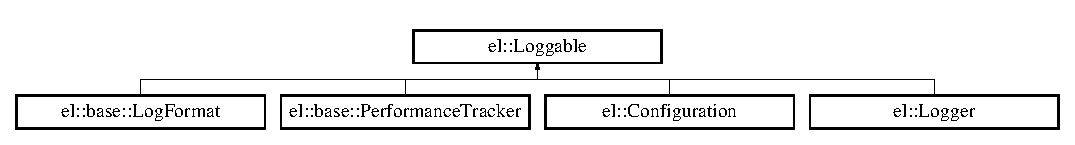
\includegraphics[height=1.505376cm]{classel_1_1_loggable}
\end{center}
\end{figure}
\subsection*{Public Member Functions}
\begin{DoxyCompactItemize}
\item 
virtual \hyperlink{classel_1_1_loggable_a6891b802d139da4041edf9e36d38e6c4}{$\sim$\+Loggable} (void)
\item 
virtual void \hyperlink{classel_1_1_loggable_ad8a2e0ebc11e4bd00ef49fc67db3d59e}{log} (\hyperlink{namespaceel_1_1base_1_1type_a74ea109bf34d1c44926837fb0830f445}{el\+::base\+::type\+::ostream\+\_\+t} \&) const =0
\end{DoxyCompactItemize}
\subsection*{Friends}
\begin{DoxyCompactItemize}
\item 
\hyperlink{namespaceel_1_1base_1_1type_a74ea109bf34d1c44926837fb0830f445}{el\+::base\+::type\+::ostream\+\_\+t} \& \hyperlink{classel_1_1_loggable_a00722a386f498be3ebece2e266fb0f05}{operator$<$$<$} (\hyperlink{namespaceel_1_1base_1_1type_a74ea109bf34d1c44926837fb0830f445}{el\+::base\+::type\+::ostream\+\_\+t} \&os, const \hyperlink{classel_1_1_loggable}{Loggable} \&loggable)
\end{DoxyCompactItemize}


\subsection{Detailed Description}
Base of Easylogging++ friendly class. 

After inheriting this class publicly, implement pure-\/virtual function {\ttfamily void \hyperlink{classel_1_1_loggable_ad8a2e0ebc11e4bd00ef49fc67db3d59e}{log(std\+::ostream\&) const}} 

Definition at line 2096 of file easylogging++.\+h.



\subsection{Constructor \& Destructor Documentation}
\hypertarget{classel_1_1_loggable_a6891b802d139da4041edf9e36d38e6c4}{}\index{el\+::\+Loggable@{el\+::\+Loggable}!````~Loggable@{$\sim$\+Loggable}}
\index{````~Loggable@{$\sim$\+Loggable}!el\+::\+Loggable@{el\+::\+Loggable}}
\subsubsection[{$\sim$\+Loggable}]{\setlength{\rightskip}{0pt plus 5cm}virtual el\+::\+Loggable\+::$\sim$\+Loggable (
\begin{DoxyParamCaption}
\item[{void}]{}
\end{DoxyParamCaption}
)\hspace{0.3cm}{\ttfamily [inline]}, {\ttfamily [virtual]}}\label{classel_1_1_loggable_a6891b802d139da4041edf9e36d38e6c4}


Definition at line 2098 of file easylogging++.\+h.



\subsection{Member Function Documentation}
\hypertarget{classel_1_1_loggable_ad8a2e0ebc11e4bd00ef49fc67db3d59e}{}\index{el\+::\+Loggable@{el\+::\+Loggable}!log@{log}}
\index{log@{log}!el\+::\+Loggable@{el\+::\+Loggable}}
\subsubsection[{log}]{\setlength{\rightskip}{0pt plus 5cm}virtual void el\+::\+Loggable\+::log (
\begin{DoxyParamCaption}
\item[{{\bf el\+::base\+::type\+::ostream\+\_\+t} \&}]{}
\end{DoxyParamCaption}
) const\hspace{0.3cm}{\ttfamily [pure virtual]}}\label{classel_1_1_loggable_ad8a2e0ebc11e4bd00ef49fc67db3d59e}


Implemented in \hyperlink{classel_1_1_logger_a12e1e5f6f91bad8d6a71c3918f09b672}{el\+::\+Logger}, \hyperlink{classel_1_1_configuration_a82c87e1a93211a1d21da99570f47dd49}{el\+::\+Configuration}, and \hyperlink{classel_1_1base_1_1_log_format_a0cae595d1a367538243feb1be1555d2e}{el\+::base\+::\+Log\+Format}.



\subsection{Friends And Related Function Documentation}
\hypertarget{classel_1_1_loggable_a00722a386f498be3ebece2e266fb0f05}{}\index{el\+::\+Loggable@{el\+::\+Loggable}!operator$<$$<$@{operator$<$$<$}}
\index{operator$<$$<$@{operator$<$$<$}!el\+::\+Loggable@{el\+::\+Loggable}}
\subsubsection[{operator$<$$<$}]{\setlength{\rightskip}{0pt plus 5cm}{\bf el\+::base\+::type\+::ostream\+\_\+t}\& operator$<$$<$ (
\begin{DoxyParamCaption}
\item[{{\bf el\+::base\+::type\+::ostream\+\_\+t} \&}]{os, }
\item[{const {\bf Loggable} \&}]{loggable}
\end{DoxyParamCaption}
)\hspace{0.3cm}{\ttfamily [friend]}}\label{classel_1_1_loggable_a00722a386f498be3ebece2e266fb0f05}


Definition at line 2101 of file easylogging++.\+h.



The documentation for this class was generated from the following file\+:\begin{DoxyCompactItemize}
\item 
lib/\hyperlink{easylogging_09_09_8h}{easylogging++.\+h}\end{DoxyCompactItemize}

\hypertarget{classel_1_1_logger}{}\section{el\+:\+:Logger Class Reference}
\label{classel_1_1_logger}\index{el\+::\+Logger@{el\+::\+Logger}}


Represents a logger holding I\+D and configurations we need to write logs.  




{\ttfamily \#include $<$easylogging++.\+h$>$}

Inheritance diagram for el\+:\+:Logger\+:\begin{figure}[H]
\begin{center}
\leavevmode
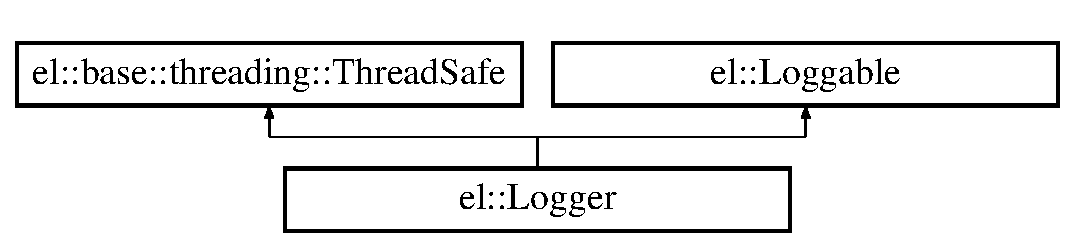
\includegraphics[height=2.000000cm]{classel_1_1_logger}
\end{center}
\end{figure}
\subsection*{Public Member Functions}
\begin{DoxyCompactItemize}
\item 
\hyperlink{classel_1_1_logger_a59b1c5a0f8c5c670e59d2f69f9e39fbb}{Logger} (const std\+::string \&\hyperlink{classel_1_1_logger_ae51a621df3c835f51f450134ba66f8ac}{id}, \hyperlink{namespaceel_1_1base_af7602da9fe1d6c75985184fb0e39fd11}{base\+::\+Log\+Streams\+Reference\+Map} $\ast$log\+Streams\+Reference)
\item 
\hyperlink{classel_1_1_logger_a43abea8865d7316f05c8a676a8c04896}{Logger} (const std\+::string \&\hyperlink{classel_1_1_logger_ae51a621df3c835f51f450134ba66f8ac}{id}, const \hyperlink{classel_1_1_configurations}{Configurations} \&\hyperlink{classel_1_1_logger_aeb57aeaddbb3dcd0cb96114019817142}{configurations}, \hyperlink{namespaceel_1_1base_af7602da9fe1d6c75985184fb0e39fd11}{base\+::\+Log\+Streams\+Reference\+Map} $\ast$log\+Streams\+Reference)
\item 
\hyperlink{classel_1_1_logger_a984de07936a8c783e91496dfa6df69ea}{Logger} (const \hyperlink{classel_1_1_logger}{Logger} \&logger)
\item 
\hyperlink{classel_1_1_logger}{Logger} \& \hyperlink{classel_1_1_logger_a2bfb4ed37f3281a701f20fb21a4cac62}{operator=} (const \hyperlink{classel_1_1_logger}{Logger} \&logger)
\item 
virtual \hyperlink{classel_1_1_logger_ae285e82b96ffcbe715ed1f9e51f2f86e}{$\sim$\+Logger} (void)
\item 
virtual void \hyperlink{classel_1_1_logger_a12e1e5f6f91bad8d6a71c3918f09b672}{log} (\hyperlink{namespaceel_1_1base_1_1type_a74ea109bf34d1c44926837fb0830f445}{el\+::base\+::type\+::ostream\+\_\+t} \&os) const 
\item 
void \hyperlink{classel_1_1_logger_ad9db621dbf8977bf814dc7baea8dcee4}{configure} (const \hyperlink{classel_1_1_configurations}{Configurations} \&\hyperlink{classel_1_1_logger_aeb57aeaddbb3dcd0cb96114019817142}{configurations})
\begin{DoxyCompactList}\small\item\em Configures the logger using specified configurations. \end{DoxyCompactList}\item 
void \hyperlink{classel_1_1_logger_adfd57ab27fb398cc980a3edfab92927e}{reconfigure} (void)
\begin{DoxyCompactList}\small\item\em Reconfigures logger using existing configurations. \end{DoxyCompactList}\item 
const std\+::string \& \hyperlink{classel_1_1_logger_ae51a621df3c835f51f450134ba66f8ac}{id} (void) const 
\item 
const std\+::string \& \hyperlink{classel_1_1_logger_a9e56e468bccd7b52281e7bbc75892431}{parent\+Application\+Name} (void) const 
\item 
void \hyperlink{classel_1_1_logger_a6890af8910adba26b01ef029429c4f15}{set\+Parent\+Application\+Name} (const std\+::string \&\hyperlink{classel_1_1_logger_a9e56e468bccd7b52281e7bbc75892431}{parent\+Application\+Name})
\item 
\hyperlink{classel_1_1_configurations}{Configurations} $\ast$ \hyperlink{classel_1_1_logger_aeb57aeaddbb3dcd0cb96114019817142}{configurations} (void)
\item 
\hyperlink{classel_1_1base_1_1_typed_configurations}{base\+::\+Typed\+Configurations} $\ast$ \hyperlink{classel_1_1_logger_ac1d34e77892ea506b011d5279b6b139d}{typed\+Configurations} (void)
\item 
void \hyperlink{classel_1_1_logger_a9a89d454008b1ee1a197eec4b92ce22a}{flush} (void)
\begin{DoxyCompactList}\small\item\em Flushes logger to sync all log files for all levels. \end{DoxyCompactList}\item 
void \hyperlink{classel_1_1_logger_a83c85278ebeeef6a24cc112e56c344dd}{flush} (\hyperlink{namespaceel_ab0ac6091262344c52dd2d3ad099e8e36}{Level} level, \hyperlink{namespaceel_1_1base_1_1type_a620c830ead75d26b45c060c211ee2685}{base\+::type\+::fstream\+\_\+t} $\ast$fs)
\item 
bool \hyperlink{classel_1_1_logger_abdf56c00388c71d1cbaa7e2df4449202}{is\+Flush\+Needed} (\hyperlink{namespaceel_ab0ac6091262344c52dd2d3ad099e8e36}{Level} level)
\item 
\hyperlink{classel_1_1_log_builder}{Log\+Builder} $\ast$ \hyperlink{classel_1_1_logger_aead5b130c5141d2024740b03ab4b45d7}{log\+Builder} (void) const 
\item 
void \hyperlink{classel_1_1_logger_a737340322cc9d9d20febd7131c1e262f}{set\+Log\+Builder} (const \hyperlink{namespaceel_ad4c4b2f7d70a4b02568a9f70724a6b39}{Log\+Builder\+Ptr} \&\hyperlink{classel_1_1_logger_aead5b130c5141d2024740b03ab4b45d7}{log\+Builder})
\item 
bool \hyperlink{classel_1_1_logger_a5abaca24ac28bfd4806bea32be193435}{enabled} (\hyperlink{namespaceel_ab0ac6091262344c52dd2d3ad099e8e36}{Level} level) const 
\end{DoxyCompactItemize}
\subsection*{Static Public Member Functions}
\begin{DoxyCompactItemize}
\item 
static bool \hyperlink{classel_1_1_logger_af6cf4f266ceb65da9563afd3706f26d6}{is\+Valid\+Id} (const std\+::string \&\hyperlink{classel_1_1_logger_ae51a621df3c835f51f450134ba66f8ac}{id})
\end{DoxyCompactItemize}
\subsection*{Friends}
\begin{DoxyCompactItemize}
\item 
class \hyperlink{classel_1_1_logger_a22965b691242a9f61d443ba03fce3e35}{el\+::\+Log\+Message}
\item 
class \hyperlink{classel_1_1_logger_a6efe246b312d02731fb0e1d120c0331d}{el\+::\+Loggers}
\item 
class \hyperlink{classel_1_1_logger_a2fb8a2c02cbf86247f093c118bed877a}{el\+::\+Helpers}
\item 
class \hyperlink{classel_1_1_logger_a574ecee25e8d578f76060a95a2fe7c9e}{el\+::base\+::\+Registered\+Loggers}
\item 
class \hyperlink{classel_1_1_logger_a42b1de96d584ae4fecbfc2b9aff95052}{el\+::base\+::\+Default\+Log\+Dispatch\+Callback}
\item 
class \hyperlink{classel_1_1_logger_a81bbf6fe31fab133d182efa8367304f1}{el\+::base\+::\+Message\+Builder}
\item 
class \hyperlink{classel_1_1_logger_a7a728edbb2761d151832daa74d5b2736}{el\+::base\+::\+Writer}
\item 
class \hyperlink{classel_1_1_logger_a2a368b9be1b8d6a29d4bb92a11807f39}{el\+::base\+::\+P\+Error\+Writer}
\item 
class \hyperlink{classel_1_1_logger_acc1efd1b8a3fc5e0028dab98b02e550a}{el\+::base\+::\+Storage}
\item 
class \hyperlink{classel_1_1_logger_a6a4d7851e1984800be3c230f06a79528}{el\+::base\+::\+Performance\+Tracker}
\item 
class \hyperlink{classel_1_1_logger_a9b37b28ea1c5f8f862cc89f135711d92}{el\+::base\+::\+Log\+Dispatcher}
\end{DoxyCompactItemize}
\subsection*{Additional Inherited Members}


\subsection{Detailed Description}
Represents a logger holding I\+D and configurations we need to write logs. 

This class does not write logs itself instead its used by writer to read configuations from. 

Definition at line 3374 of file easylogging++.\+h.



\subsection{Constructor \& Destructor Documentation}
\hypertarget{classel_1_1_logger_a59b1c5a0f8c5c670e59d2f69f9e39fbb}{}\index{el\+::\+Logger@{el\+::\+Logger}!Logger@{Logger}}
\index{Logger@{Logger}!el\+::\+Logger@{el\+::\+Logger}}
\subsubsection[{Logger}]{\setlength{\rightskip}{0pt plus 5cm}el\+::\+Logger\+::\+Logger (
\begin{DoxyParamCaption}
\item[{const std\+::string \&}]{id, }
\item[{{\bf base\+::\+Log\+Streams\+Reference\+Map} $\ast$}]{log\+Streams\+Reference}
\end{DoxyParamCaption}
)\hspace{0.3cm}{\ttfamily [inline]}}\label{classel_1_1_logger_a59b1c5a0f8c5c670e59d2f69f9e39fbb}


Definition at line 3376 of file easylogging++.\+h.

\hypertarget{classel_1_1_logger_a43abea8865d7316f05c8a676a8c04896}{}\index{el\+::\+Logger@{el\+::\+Logger}!Logger@{Logger}}
\index{Logger@{Logger}!el\+::\+Logger@{el\+::\+Logger}}
\subsubsection[{Logger}]{\setlength{\rightskip}{0pt plus 5cm}el\+::\+Logger\+::\+Logger (
\begin{DoxyParamCaption}
\item[{const std\+::string \&}]{id, }
\item[{const {\bf Configurations} \&}]{configurations, }
\item[{{\bf base\+::\+Log\+Streams\+Reference\+Map} $\ast$}]{log\+Streams\+Reference}
\end{DoxyParamCaption}
)\hspace{0.3cm}{\ttfamily [inline]}}\label{classel_1_1_logger_a43abea8865d7316f05c8a676a8c04896}


Definition at line 3385 of file easylogging++.\+h.

\hypertarget{classel_1_1_logger_a984de07936a8c783e91496dfa6df69ea}{}\index{el\+::\+Logger@{el\+::\+Logger}!Logger@{Logger}}
\index{Logger@{Logger}!el\+::\+Logger@{el\+::\+Logger}}
\subsubsection[{Logger}]{\setlength{\rightskip}{0pt plus 5cm}el\+::\+Logger\+::\+Logger (
\begin{DoxyParamCaption}
\item[{const {\bf Logger} \&}]{logger}
\end{DoxyParamCaption}
)\hspace{0.3cm}{\ttfamily [inline]}}\label{classel_1_1_logger_a984de07936a8c783e91496dfa6df69ea}


Definition at line 3395 of file easylogging++.\+h.

\hypertarget{classel_1_1_logger_ae285e82b96ffcbe715ed1f9e51f2f86e}{}\index{el\+::\+Logger@{el\+::\+Logger}!````~Logger@{$\sim$\+Logger}}
\index{````~Logger@{$\sim$\+Logger}!el\+::\+Logger@{el\+::\+Logger}}
\subsubsection[{$\sim$\+Logger}]{\setlength{\rightskip}{0pt plus 5cm}virtual el\+::\+Logger\+::$\sim$\+Logger (
\begin{DoxyParamCaption}
\item[{void}]{}
\end{DoxyParamCaption}
)\hspace{0.3cm}{\ttfamily [inline]}, {\ttfamily [virtual]}}\label{classel_1_1_logger_ae285e82b96ffcbe715ed1f9e51f2f86e}


Definition at line 3418 of file easylogging++.\+h.



\subsection{Member Function Documentation}
\hypertarget{classel_1_1_logger_aeb57aeaddbb3dcd0cb96114019817142}{}\index{el\+::\+Logger@{el\+::\+Logger}!configurations@{configurations}}
\index{configurations@{configurations}!el\+::\+Logger@{el\+::\+Logger}}
\subsubsection[{configurations}]{\setlength{\rightskip}{0pt plus 5cm}{\bf Configurations}$\ast$ el\+::\+Logger\+::configurations (
\begin{DoxyParamCaption}
\item[{void}]{}
\end{DoxyParamCaption}
)\hspace{0.3cm}{\ttfamily [inline]}}\label{classel_1_1_logger_aeb57aeaddbb3dcd0cb96114019817142}


Definition at line 3465 of file easylogging++.\+h.

\hypertarget{classel_1_1_logger_ad9db621dbf8977bf814dc7baea8dcee4}{}\index{el\+::\+Logger@{el\+::\+Logger}!configure@{configure}}
\index{configure@{configure}!el\+::\+Logger@{el\+::\+Logger}}
\subsubsection[{configure}]{\setlength{\rightskip}{0pt plus 5cm}void el\+::\+Logger\+::configure (
\begin{DoxyParamCaption}
\item[{const {\bf Configurations} \&}]{configurations}
\end{DoxyParamCaption}
)\hspace{0.3cm}{\ttfamily [inline]}}\label{classel_1_1_logger_ad9db621dbf8977bf814dc7baea8dcee4}


Configures the logger using specified configurations. 



Definition at line 3427 of file easylogging++.\+h.

\hypertarget{classel_1_1_logger_a5abaca24ac28bfd4806bea32be193435}{}\index{el\+::\+Logger@{el\+::\+Logger}!enabled@{enabled}}
\index{enabled@{enabled}!el\+::\+Logger@{el\+::\+Logger}}
\subsubsection[{enabled}]{\setlength{\rightskip}{0pt plus 5cm}bool el\+::\+Logger\+::enabled (
\begin{DoxyParamCaption}
\item[{{\bf Level}}]{level}
\end{DoxyParamCaption}
) const\hspace{0.3cm}{\ttfamily [inline]}}\label{classel_1_1_logger_a5abaca24ac28bfd4806bea32be193435}


Definition at line 3514 of file easylogging++.\+h.

\hypertarget{classel_1_1_logger_a9a89d454008b1ee1a197eec4b92ce22a}{}\index{el\+::\+Logger@{el\+::\+Logger}!flush@{flush}}
\index{flush@{flush}!el\+::\+Logger@{el\+::\+Logger}}
\subsubsection[{flush}]{\setlength{\rightskip}{0pt plus 5cm}void el\+::\+Logger\+::flush (
\begin{DoxyParamCaption}
\item[{void}]{}
\end{DoxyParamCaption}
)\hspace{0.3cm}{\ttfamily [inline]}}\label{classel_1_1_logger_a9a89d454008b1ee1a197eec4b92ce22a}


Flushes logger to sync all log files for all levels. 



Definition at line 3482 of file easylogging++.\+h.

\hypertarget{classel_1_1_logger_a83c85278ebeeef6a24cc112e56c344dd}{}\index{el\+::\+Logger@{el\+::\+Logger}!flush@{flush}}
\index{flush@{flush}!el\+::\+Logger@{el\+::\+Logger}}
\subsubsection[{flush}]{\setlength{\rightskip}{0pt plus 5cm}void el\+::\+Logger\+::flush (
\begin{DoxyParamCaption}
\item[{{\bf Level}}]{level, }
\item[{{\bf base\+::type\+::fstream\+\_\+t} $\ast$}]{fs}
\end{DoxyParamCaption}
)\hspace{0.3cm}{\ttfamily [inline]}}\label{classel_1_1_logger_a83c85278ebeeef6a24cc112e56c344dd}


Definition at line 3492 of file easylogging++.\+h.

\hypertarget{classel_1_1_logger_ae51a621df3c835f51f450134ba66f8ac}{}\index{el\+::\+Logger@{el\+::\+Logger}!id@{id}}
\index{id@{id}!el\+::\+Logger@{el\+::\+Logger}}
\subsubsection[{id}]{\setlength{\rightskip}{0pt plus 5cm}const std\+::string\& el\+::\+Logger\+::id (
\begin{DoxyParamCaption}
\item[{void}]{}
\end{DoxyParamCaption}
) const\hspace{0.3cm}{\ttfamily [inline]}}\label{classel_1_1_logger_ae51a621df3c835f51f450134ba66f8ac}


Definition at line 3453 of file easylogging++.\+h.

\hypertarget{classel_1_1_logger_abdf56c00388c71d1cbaa7e2df4449202}{}\index{el\+::\+Logger@{el\+::\+Logger}!is\+Flush\+Needed@{is\+Flush\+Needed}}
\index{is\+Flush\+Needed@{is\+Flush\+Needed}!el\+::\+Logger@{el\+::\+Logger}}
\subsubsection[{is\+Flush\+Needed}]{\setlength{\rightskip}{0pt plus 5cm}bool el\+::\+Logger\+::is\+Flush\+Needed (
\begin{DoxyParamCaption}
\item[{{\bf Level}}]{level}
\end{DoxyParamCaption}
)\hspace{0.3cm}{\ttfamily [inline]}}\label{classel_1_1_logger_abdf56c00388c71d1cbaa7e2df4449202}


Definition at line 3502 of file easylogging++.\+h.

\hypertarget{classel_1_1_logger_af6cf4f266ceb65da9563afd3706f26d6}{}\index{el\+::\+Logger@{el\+::\+Logger}!is\+Valid\+Id@{is\+Valid\+Id}}
\index{is\+Valid\+Id@{is\+Valid\+Id}!el\+::\+Logger@{el\+::\+Logger}}
\subsubsection[{is\+Valid\+Id}]{\setlength{\rightskip}{0pt plus 5cm}static bool el\+::\+Logger\+::is\+Valid\+Id (
\begin{DoxyParamCaption}
\item[{const std\+::string \&}]{id}
\end{DoxyParamCaption}
)\hspace{0.3cm}{\ttfamily [inline]}, {\ttfamily [static]}}\label{classel_1_1_logger_af6cf4f266ceb65da9563afd3706f26d6}


Definition at line 3473 of file easylogging++.\+h.

\hypertarget{classel_1_1_logger_a12e1e5f6f91bad8d6a71c3918f09b672}{}\index{el\+::\+Logger@{el\+::\+Logger}!log@{log}}
\index{log@{log}!el\+::\+Logger@{el\+::\+Logger}}
\subsubsection[{log}]{\setlength{\rightskip}{0pt plus 5cm}virtual void el\+::\+Logger\+::log (
\begin{DoxyParamCaption}
\item[{{\bf el\+::base\+::type\+::ostream\+\_\+t} \&}]{os}
\end{DoxyParamCaption}
) const\hspace{0.3cm}{\ttfamily [inline]}, {\ttfamily [virtual]}}\label{classel_1_1_logger_a12e1e5f6f91bad8d6a71c3918f09b672}


Implements \hyperlink{classel_1_1_loggable_ad8a2e0ebc11e4bd00ef49fc67db3d59e}{el\+::\+Loggable}.



Definition at line 3422 of file easylogging++.\+h.

\hypertarget{classel_1_1_logger_aead5b130c5141d2024740b03ab4b45d7}{}\index{el\+::\+Logger@{el\+::\+Logger}!log\+Builder@{log\+Builder}}
\index{log\+Builder@{log\+Builder}!el\+::\+Logger@{el\+::\+Logger}}
\subsubsection[{log\+Builder}]{\setlength{\rightskip}{0pt plus 5cm}{\bf Log\+Builder}$\ast$ el\+::\+Logger\+::log\+Builder (
\begin{DoxyParamCaption}
\item[{void}]{}
\end{DoxyParamCaption}
) const\hspace{0.3cm}{\ttfamily [inline]}}\label{classel_1_1_logger_aead5b130c5141d2024740b03ab4b45d7}


Definition at line 3506 of file easylogging++.\+h.

\hypertarget{classel_1_1_logger_a2bfb4ed37f3281a701f20fb21a4cac62}{}\index{el\+::\+Logger@{el\+::\+Logger}!operator=@{operator=}}
\index{operator=@{operator=}!el\+::\+Logger@{el\+::\+Logger}}
\subsubsection[{operator=}]{\setlength{\rightskip}{0pt plus 5cm}{\bf Logger}\& el\+::\+Logger\+::operator= (
\begin{DoxyParamCaption}
\item[{const {\bf Logger} \&}]{logger}
\end{DoxyParamCaption}
)\hspace{0.3cm}{\ttfamily [inline]}}\label{classel_1_1_logger_a2bfb4ed37f3281a701f20fb21a4cac62}


Definition at line 3406 of file easylogging++.\+h.

\hypertarget{classel_1_1_logger_a9e56e468bccd7b52281e7bbc75892431}{}\index{el\+::\+Logger@{el\+::\+Logger}!parent\+Application\+Name@{parent\+Application\+Name}}
\index{parent\+Application\+Name@{parent\+Application\+Name}!el\+::\+Logger@{el\+::\+Logger}}
\subsubsection[{parent\+Application\+Name}]{\setlength{\rightskip}{0pt plus 5cm}const std\+::string\& el\+::\+Logger\+::parent\+Application\+Name (
\begin{DoxyParamCaption}
\item[{void}]{}
\end{DoxyParamCaption}
) const\hspace{0.3cm}{\ttfamily [inline]}}\label{classel_1_1_logger_a9e56e468bccd7b52281e7bbc75892431}


Definition at line 3457 of file easylogging++.\+h.

\hypertarget{classel_1_1_logger_adfd57ab27fb398cc980a3edfab92927e}{}\index{el\+::\+Logger@{el\+::\+Logger}!reconfigure@{reconfigure}}
\index{reconfigure@{reconfigure}!el\+::\+Logger@{el\+::\+Logger}}
\subsubsection[{reconfigure}]{\setlength{\rightskip}{0pt plus 5cm}void el\+::\+Logger\+::reconfigure (
\begin{DoxyParamCaption}
\item[{void}]{}
\end{DoxyParamCaption}
)\hspace{0.3cm}{\ttfamily [inline]}}\label{classel_1_1_logger_adfd57ab27fb398cc980a3edfab92927e}


Reconfigures logger using existing configurations. 



Definition at line 3448 of file easylogging++.\+h.

\hypertarget{classel_1_1_logger_a737340322cc9d9d20febd7131c1e262f}{}\index{el\+::\+Logger@{el\+::\+Logger}!set\+Log\+Builder@{set\+Log\+Builder}}
\index{set\+Log\+Builder@{set\+Log\+Builder}!el\+::\+Logger@{el\+::\+Logger}}
\subsubsection[{set\+Log\+Builder}]{\setlength{\rightskip}{0pt plus 5cm}void el\+::\+Logger\+::set\+Log\+Builder (
\begin{DoxyParamCaption}
\item[{const {\bf Log\+Builder\+Ptr} \&}]{log\+Builder}
\end{DoxyParamCaption}
)\hspace{0.3cm}{\ttfamily [inline]}}\label{classel_1_1_logger_a737340322cc9d9d20febd7131c1e262f}


Definition at line 3510 of file easylogging++.\+h.

\hypertarget{classel_1_1_logger_a6890af8910adba26b01ef029429c4f15}{}\index{el\+::\+Logger@{el\+::\+Logger}!set\+Parent\+Application\+Name@{set\+Parent\+Application\+Name}}
\index{set\+Parent\+Application\+Name@{set\+Parent\+Application\+Name}!el\+::\+Logger@{el\+::\+Logger}}
\subsubsection[{set\+Parent\+Application\+Name}]{\setlength{\rightskip}{0pt plus 5cm}void el\+::\+Logger\+::set\+Parent\+Application\+Name (
\begin{DoxyParamCaption}
\item[{const std\+::string \&}]{parent\+Application\+Name}
\end{DoxyParamCaption}
)\hspace{0.3cm}{\ttfamily [inline]}}\label{classel_1_1_logger_a6890af8910adba26b01ef029429c4f15}


Definition at line 3461 of file easylogging++.\+h.

\hypertarget{classel_1_1_logger_ac1d34e77892ea506b011d5279b6b139d}{}\index{el\+::\+Logger@{el\+::\+Logger}!typed\+Configurations@{typed\+Configurations}}
\index{typed\+Configurations@{typed\+Configurations}!el\+::\+Logger@{el\+::\+Logger}}
\subsubsection[{typed\+Configurations}]{\setlength{\rightskip}{0pt plus 5cm}{\bf base\+::\+Typed\+Configurations}$\ast$ el\+::\+Logger\+::typed\+Configurations (
\begin{DoxyParamCaption}
\item[{void}]{}
\end{DoxyParamCaption}
)\hspace{0.3cm}{\ttfamily [inline]}}\label{classel_1_1_logger_ac1d34e77892ea506b011d5279b6b139d}


Definition at line 3469 of file easylogging++.\+h.



\subsection{Friends And Related Function Documentation}
\hypertarget{classel_1_1_logger_a42b1de96d584ae4fecbfc2b9aff95052}{}\index{el\+::\+Logger@{el\+::\+Logger}!el\+::base\+::\+Default\+Log\+Dispatch\+Callback@{el\+::base\+::\+Default\+Log\+Dispatch\+Callback}}
\index{el\+::base\+::\+Default\+Log\+Dispatch\+Callback@{el\+::base\+::\+Default\+Log\+Dispatch\+Callback}!el\+::\+Logger@{el\+::\+Logger}}
\subsubsection[{el\+::base\+::\+Default\+Log\+Dispatch\+Callback}]{\setlength{\rightskip}{0pt plus 5cm}friend class {\bf el\+::base\+::\+Default\+Log\+Dispatch\+Callback}\hspace{0.3cm}{\ttfamily [friend]}}\label{classel_1_1_logger_a42b1de96d584ae4fecbfc2b9aff95052}


Definition at line 3554 of file easylogging++.\+h.

\hypertarget{classel_1_1_logger_a9b37b28ea1c5f8f862cc89f135711d92}{}\index{el\+::\+Logger@{el\+::\+Logger}!el\+::base\+::\+Log\+Dispatcher@{el\+::base\+::\+Log\+Dispatcher}}
\index{el\+::base\+::\+Log\+Dispatcher@{el\+::base\+::\+Log\+Dispatcher}!el\+::\+Logger@{el\+::\+Logger}}
\subsubsection[{el\+::base\+::\+Log\+Dispatcher}]{\setlength{\rightskip}{0pt plus 5cm}friend class {\bf el\+::base\+::\+Log\+Dispatcher}\hspace{0.3cm}{\ttfamily [friend]}}\label{classel_1_1_logger_a9b37b28ea1c5f8f862cc89f135711d92}


Definition at line 3560 of file easylogging++.\+h.

\hypertarget{classel_1_1_logger_a81bbf6fe31fab133d182efa8367304f1}{}\index{el\+::\+Logger@{el\+::\+Logger}!el\+::base\+::\+Message\+Builder@{el\+::base\+::\+Message\+Builder}}
\index{el\+::base\+::\+Message\+Builder@{el\+::base\+::\+Message\+Builder}!el\+::\+Logger@{el\+::\+Logger}}
\subsubsection[{el\+::base\+::\+Message\+Builder}]{\setlength{\rightskip}{0pt plus 5cm}friend class {\bf el\+::base\+::\+Message\+Builder}\hspace{0.3cm}{\ttfamily [friend]}}\label{classel_1_1_logger_a81bbf6fe31fab133d182efa8367304f1}


Definition at line 3555 of file easylogging++.\+h.

\hypertarget{classel_1_1_logger_a6a4d7851e1984800be3c230f06a79528}{}\index{el\+::\+Logger@{el\+::\+Logger}!el\+::base\+::\+Performance\+Tracker@{el\+::base\+::\+Performance\+Tracker}}
\index{el\+::base\+::\+Performance\+Tracker@{el\+::base\+::\+Performance\+Tracker}!el\+::\+Logger@{el\+::\+Logger}}
\subsubsection[{el\+::base\+::\+Performance\+Tracker}]{\setlength{\rightskip}{0pt plus 5cm}friend class {\bf el\+::base\+::\+Performance\+Tracker}\hspace{0.3cm}{\ttfamily [friend]}}\label{classel_1_1_logger_a6a4d7851e1984800be3c230f06a79528}


Definition at line 3559 of file easylogging++.\+h.

\hypertarget{classel_1_1_logger_a2a368b9be1b8d6a29d4bb92a11807f39}{}\index{el\+::\+Logger@{el\+::\+Logger}!el\+::base\+::\+P\+Error\+Writer@{el\+::base\+::\+P\+Error\+Writer}}
\index{el\+::base\+::\+P\+Error\+Writer@{el\+::base\+::\+P\+Error\+Writer}!el\+::\+Logger@{el\+::\+Logger}}
\subsubsection[{el\+::base\+::\+P\+Error\+Writer}]{\setlength{\rightskip}{0pt plus 5cm}friend class {\bf el\+::base\+::\+P\+Error\+Writer}\hspace{0.3cm}{\ttfamily [friend]}}\label{classel_1_1_logger_a2a368b9be1b8d6a29d4bb92a11807f39}


Definition at line 3557 of file easylogging++.\+h.

\hypertarget{classel_1_1_logger_a574ecee25e8d578f76060a95a2fe7c9e}{}\index{el\+::\+Logger@{el\+::\+Logger}!el\+::base\+::\+Registered\+Loggers@{el\+::base\+::\+Registered\+Loggers}}
\index{el\+::base\+::\+Registered\+Loggers@{el\+::base\+::\+Registered\+Loggers}!el\+::\+Logger@{el\+::\+Logger}}
\subsubsection[{el\+::base\+::\+Registered\+Loggers}]{\setlength{\rightskip}{0pt plus 5cm}friend class {\bf el\+::base\+::\+Registered\+Loggers}\hspace{0.3cm}{\ttfamily [friend]}}\label{classel_1_1_logger_a574ecee25e8d578f76060a95a2fe7c9e}


Definition at line 3553 of file easylogging++.\+h.

\hypertarget{classel_1_1_logger_acc1efd1b8a3fc5e0028dab98b02e550a}{}\index{el\+::\+Logger@{el\+::\+Logger}!el\+::base\+::\+Storage@{el\+::base\+::\+Storage}}
\index{el\+::base\+::\+Storage@{el\+::base\+::\+Storage}!el\+::\+Logger@{el\+::\+Logger}}
\subsubsection[{el\+::base\+::\+Storage}]{\setlength{\rightskip}{0pt plus 5cm}friend class {\bf el\+::base\+::\+Storage}\hspace{0.3cm}{\ttfamily [friend]}}\label{classel_1_1_logger_acc1efd1b8a3fc5e0028dab98b02e550a}


Definition at line 3558 of file easylogging++.\+h.

\hypertarget{classel_1_1_logger_a7a728edbb2761d151832daa74d5b2736}{}\index{el\+::\+Logger@{el\+::\+Logger}!el\+::base\+::\+Writer@{el\+::base\+::\+Writer}}
\index{el\+::base\+::\+Writer@{el\+::base\+::\+Writer}!el\+::\+Logger@{el\+::\+Logger}}
\subsubsection[{el\+::base\+::\+Writer}]{\setlength{\rightskip}{0pt plus 5cm}friend class {\bf el\+::base\+::\+Writer}\hspace{0.3cm}{\ttfamily [friend]}}\label{classel_1_1_logger_a7a728edbb2761d151832daa74d5b2736}


Definition at line 3556 of file easylogging++.\+h.

\hypertarget{classel_1_1_logger_a2fb8a2c02cbf86247f093c118bed877a}{}\index{el\+::\+Logger@{el\+::\+Logger}!el\+::\+Helpers@{el\+::\+Helpers}}
\index{el\+::\+Helpers@{el\+::\+Helpers}!el\+::\+Logger@{el\+::\+Logger}}
\subsubsection[{el\+::\+Helpers}]{\setlength{\rightskip}{0pt plus 5cm}friend class {\bf el\+::\+Helpers}\hspace{0.3cm}{\ttfamily [friend]}}\label{classel_1_1_logger_a2fb8a2c02cbf86247f093c118bed877a}


Definition at line 3552 of file easylogging++.\+h.

\hypertarget{classel_1_1_logger_a6efe246b312d02731fb0e1d120c0331d}{}\index{el\+::\+Logger@{el\+::\+Logger}!el\+::\+Loggers@{el\+::\+Loggers}}
\index{el\+::\+Loggers@{el\+::\+Loggers}!el\+::\+Logger@{el\+::\+Logger}}
\subsubsection[{el\+::\+Loggers}]{\setlength{\rightskip}{0pt plus 5cm}friend class {\bf el\+::\+Loggers}\hspace{0.3cm}{\ttfamily [friend]}}\label{classel_1_1_logger_a6efe246b312d02731fb0e1d120c0331d}


Definition at line 3551 of file easylogging++.\+h.

\hypertarget{classel_1_1_logger_a22965b691242a9f61d443ba03fce3e35}{}\index{el\+::\+Logger@{el\+::\+Logger}!el\+::\+Log\+Message@{el\+::\+Log\+Message}}
\index{el\+::\+Log\+Message@{el\+::\+Log\+Message}!el\+::\+Logger@{el\+::\+Logger}}
\subsubsection[{el\+::\+Log\+Message}]{\setlength{\rightskip}{0pt plus 5cm}friend class {\bf el\+::\+Log\+Message}\hspace{0.3cm}{\ttfamily [friend]}}\label{classel_1_1_logger_a22965b691242a9f61d443ba03fce3e35}


Definition at line 3550 of file easylogging++.\+h.



The documentation for this class was generated from the following file\+:\begin{DoxyCompactItemize}
\item 
lib/\hyperlink{easylogging_09_09_8h}{easylogging++.\+h}\end{DoxyCompactItemize}

\hypertarget{classel_1_1_loggers}{}\section{el\+:\+:Loggers Class Reference}
\label{classel_1_1_loggers}\index{el\+::\+Loggers@{el\+::\+Loggers}}


Static helpers to deal with loggers and their configurations.  




{\ttfamily \#include $<$easylogging++.\+h$>$}

Inheritance diagram for el\+:\+:Loggers\+:\begin{figure}[H]
\begin{center}
\leavevmode
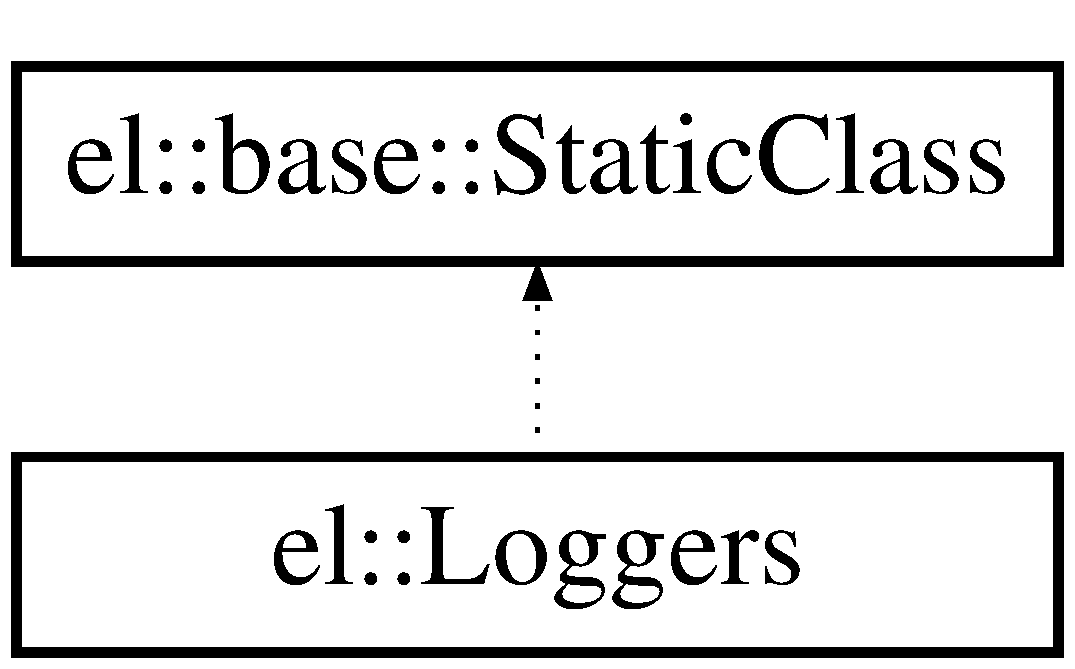
\includegraphics[height=2.000000cm]{classel_1_1_loggers}
\end{center}
\end{figure}
\subsection*{Classes}
\begin{DoxyCompactItemize}
\item 
class \hyperlink{classel_1_1_loggers_1_1_scoped_add_flag}{Scoped\+Add\+Flag}
\begin{DoxyCompactList}\small\item\em Adds flag and removes it when scope goes out. \end{DoxyCompactList}\item 
class \hyperlink{classel_1_1_loggers_1_1_scoped_remove_flag}{Scoped\+Remove\+Flag}
\begin{DoxyCompactList}\small\item\em Removes flag and add it when scope goes out. \end{DoxyCompactList}\end{DoxyCompactItemize}
\subsection*{Static Public Member Functions}
\begin{DoxyCompactItemize}
\item 
static \hyperlink{classel_1_1_logger}{Logger} $\ast$ \hyperlink{classel_1_1_loggers_aaebf868c558e3ba1d2e4f073a00f1d4a}{get\+Logger} (const std\+::string \&identity, bool register\+If\+Not\+Available=true)
\begin{DoxyCompactList}\small\item\em Gets existing or registers new logger. \end{DoxyCompactList}\item 
static bool \hyperlink{classel_1_1_loggers_a201d261ea57c070f07f0bf2006158587}{unregister\+Logger} (const std\+::string \&identity)
\begin{DoxyCompactList}\small\item\em Unregisters logger -\/ use it only when you know what you are doing, you may unregister loggers initialized / used by third-\/party libs. \end{DoxyCompactList}\item 
static bool \hyperlink{classel_1_1_loggers_a2d7a056cb7d9da3d96c709a2fac5c2bb}{has\+Logger} (const std\+::string \&identity)
\begin{DoxyCompactList}\small\item\em Whether or not logger with id is registered. \end{DoxyCompactList}\item 
static \hyperlink{classel_1_1_logger}{Logger} $\ast$ \hyperlink{classel_1_1_loggers_a888aca5bdccccc322da2eed430909d04}{reconfigure\+Logger} (\hyperlink{classel_1_1_logger}{Logger} $\ast$logger, const \hyperlink{classel_1_1_configurations}{Configurations} \&configurations)
\begin{DoxyCompactList}\small\item\em Reconfigures specified logger with new configurations. \end{DoxyCompactList}\item 
static \hyperlink{classel_1_1_logger}{Logger} $\ast$ \hyperlink{classel_1_1_loggers_a105f776fe19cb7fa2fccd2993d9f7a7c}{reconfigure\+Logger} (const std\+::string \&identity, const \hyperlink{classel_1_1_configurations}{Configurations} \&configurations)
\begin{DoxyCompactList}\small\item\em Reconfigures logger with new configurations after looking it up using identity. \end{DoxyCompactList}\item 
static \hyperlink{classel_1_1_logger}{Logger} $\ast$ \hyperlink{classel_1_1_loggers_aef49fdae329cefcc1c01428568dced4b}{reconfigure\+Logger} (const std\+::string \&identity, \hyperlink{namespaceel_a281f5db6d6163678bc68a8b23b59e124}{Configuration\+Type} configuration\+Type, const std\+::string \&value)
\begin{DoxyCompactList}\small\item\em Reconfigures logger\textquotesingle{}s single configuration. \end{DoxyCompactList}\item 
static void \hyperlink{classel_1_1_loggers_ac834df0f5e9e3dab18e70321a2543af7}{reconfigure\+All\+Loggers} (const \hyperlink{classel_1_1_configurations}{Configurations} \&configurations)
\begin{DoxyCompactList}\small\item\em Reconfigures all the existing loggers with new configurations. \end{DoxyCompactList}\item 
static void \hyperlink{classel_1_1_loggers_a1ebd33bc0208b430f41508e34509c7c9}{reconfigure\+All\+Loggers} (\hyperlink{namespaceel_a281f5db6d6163678bc68a8b23b59e124}{Configuration\+Type} configuration\+Type, const std\+::string \&value)
\begin{DoxyCompactList}\small\item\em Reconfigures single configuration for all the loggers. \end{DoxyCompactList}\item 
static void \hyperlink{classel_1_1_loggers_ab24b99e5bb3c907d1418ee3266f15397}{reconfigure\+All\+Loggers} (\hyperlink{namespaceel_ab0ac6091262344c52dd2d3ad099e8e36}{Level} level, \hyperlink{namespaceel_a281f5db6d6163678bc68a8b23b59e124}{Configuration\+Type} configuration\+Type, const std\+::string \&value)
\begin{DoxyCompactList}\small\item\em Reconfigures single configuration for all the loggers for specified level. \end{DoxyCompactList}\item 
static void \hyperlink{classel_1_1_loggers_ab9fb62a8ff904ff887fefde3282f46a4}{set\+Default\+Configurations} (const \hyperlink{classel_1_1_configurations}{Configurations} \&configurations, bool reconfigure\+Existing\+Loggers=false)
\begin{DoxyCompactList}\small\item\em Sets default configurations. This configuration is used for future (and conditionally for existing) loggers. \end{DoxyCompactList}\item 
static const \hyperlink{classel_1_1_configurations}{Configurations} $\ast$ \hyperlink{classel_1_1_loggers_a96f2336fafdc3ef2c4df01a73ae5ffb7}{default\+Configurations} (void)
\begin{DoxyCompactList}\small\item\em Returns current default. \end{DoxyCompactList}\item 
static const \hyperlink{namespaceel_1_1base_af7602da9fe1d6c75985184fb0e39fd11}{base\+::\+Log\+Streams\+Reference\+Map} $\ast$ \hyperlink{classel_1_1_loggers_ad17312c9474d94bc98efcaf08ca279a4}{log\+Streams\+Reference} (void)
\begin{DoxyCompactList}\small\item\em Returns log stream reference pointer if needed by user. \end{DoxyCompactList}\item 
static \hyperlink{classel_1_1base_1_1_typed_configurations}{base\+::\+Typed\+Configurations} \hyperlink{classel_1_1_loggers_af296007c3eb3b71602ec80ff59875b46}{default\+Typed\+Configurations} (void)
\begin{DoxyCompactList}\small\item\em Default typed configuration based on existing default\+Conf. \end{DoxyCompactList}\item 
static std\+::vector$<$ std\+::string $>$ $\ast$ \hyperlink{classel_1_1_loggers_adea07ec6cbc1dfc50f939d69dcac7160}{populate\+All\+Logger\+Ids} (std\+::vector$<$ std\+::string $>$ $\ast$target\+List)
\begin{DoxyCompactList}\small\item\em Populates all logger I\+Ds in current repository. \end{DoxyCompactList}\item 
static void \hyperlink{classel_1_1_loggers_a9992995a85745639aa9aa5a2df2255f5}{configure\+From\+Global} (const char $\ast$global\+Configuration\+File\+Path)
\begin{DoxyCompactList}\small\item\em Sets configurations from global configuration file. \end{DoxyCompactList}\item 
static bool \hyperlink{classel_1_1_loggers_a28acf6f2b1ea7e5edd1b2560cde82406}{configure\+From\+Arg} (const char $\ast$arg\+Key)
\begin{DoxyCompactList}\small\item\em Configures loggers using command line arg. Ensure you have already set command line args,. \end{DoxyCompactList}\item 
static void \hyperlink{classel_1_1_loggers_a1834480e970c16817459ca3ee26b44b5}{flush\+All} (void)
\begin{DoxyCompactList}\small\item\em Flushes all loggers for all levels -\/ Be careful if you dont know how many loggers are registered. \end{DoxyCompactList}\item 
static void \hyperlink{classel_1_1_loggers_aedd2de02dd701b0f20ddaa10f1f728f1}{add\+Flag} (\hyperlink{namespaceel_a2784aacd04cb7816ac1c0b20fcbf83cb}{Logging\+Flag} flag)
\begin{DoxyCompactList}\small\item\em Adds logging flag used internally. \end{DoxyCompactList}\item 
static void \hyperlink{classel_1_1_loggers_a23fcb4b492f70a34285c45c0b5e2e515}{remove\+Flag} (\hyperlink{namespaceel_a2784aacd04cb7816ac1c0b20fcbf83cb}{Logging\+Flag} flag)
\begin{DoxyCompactList}\small\item\em Removes logging flag used internally. \end{DoxyCompactList}\item 
static bool \hyperlink{classel_1_1_loggers_a591a45565c1eb7073ec3a979df8b5a4c}{has\+Flag} (\hyperlink{namespaceel_a2784aacd04cb7816ac1c0b20fcbf83cb}{Logging\+Flag} flag)
\begin{DoxyCompactList}\small\item\em Determines whether or not certain flag is active. \end{DoxyCompactList}\item 
static void \hyperlink{classel_1_1_loggers_afbee019d722fef5148d8355f45ba7993}{set\+Logging\+Level} (\hyperlink{namespaceel_ab0ac6091262344c52dd2d3ad099e8e36}{Level} level)
\begin{DoxyCompactList}\small\item\em Sets hierarchy for logging. Needs to enable logging flag (Hierarchical\+Logging) \end{DoxyCompactList}\item 
static void \hyperlink{classel_1_1_loggers_a826b238fe4f3719305a2d19f0c121fa0}{set\+Verbose\+Level} (\hyperlink{namespaceel_1_1base_1_1type_a3f79fa74639a13c32f794ba074fe7fb4}{base\+::type\+::\+Verbose\+Level} level)
\begin{DoxyCompactList}\small\item\em Sets verbose level on the fly. \end{DoxyCompactList}\item 
static \hyperlink{namespaceel_1_1base_1_1type_a3f79fa74639a13c32f794ba074fe7fb4}{base\+::type\+::\+Verbose\+Level} \hyperlink{classel_1_1_loggers_ad4840bb4b6b80746a2212cf3cc058142}{verbose\+Level} (void)
\begin{DoxyCompactList}\small\item\em Gets current verbose level. \end{DoxyCompactList}\item 
static void \hyperlink{classel_1_1_loggers_acbc5e2cef230331c57f364852a671507}{set\+V\+Modules} (const char $\ast$modules)
\begin{DoxyCompactList}\small\item\em Sets vmodules as specified (on the fly) \end{DoxyCompactList}\item 
static void \hyperlink{classel_1_1_loggers_afcf50abc11530eb7f28fcab7eab27e4f}{clear\+V\+Modules} (void)
\begin{DoxyCompactList}\small\item\em Clears vmodules. \end{DoxyCompactList}\end{DoxyCompactItemize}


\subsection{Detailed Description}
Static helpers to deal with loggers and their configurations. 

Definition at line 5776 of file easylogging++.\+h.



\subsection{Member Function Documentation}
\hypertarget{classel_1_1_loggers_aedd2de02dd701b0f20ddaa10f1f728f1}{}\index{el\+::\+Loggers@{el\+::\+Loggers}!add\+Flag@{add\+Flag}}
\index{add\+Flag@{add\+Flag}!el\+::\+Loggers@{el\+::\+Loggers}}
\subsubsection[{add\+Flag}]{\setlength{\rightskip}{0pt plus 5cm}static void el\+::\+Loggers\+::add\+Flag (
\begin{DoxyParamCaption}
\item[{{\bf Logging\+Flag}}]{flag}
\end{DoxyParamCaption}
)\hspace{0.3cm}{\ttfamily [inline]}, {\ttfamily [static]}}\label{classel_1_1_loggers_aedd2de02dd701b0f20ddaa10f1f728f1}


Adds logging flag used internally. 



Definition at line 5928 of file easylogging++.\+h.

\hypertarget{classel_1_1_loggers_afcf50abc11530eb7f28fcab7eab27e4f}{}\index{el\+::\+Loggers@{el\+::\+Loggers}!clear\+V\+Modules@{clear\+V\+Modules}}
\index{clear\+V\+Modules@{clear\+V\+Modules}!el\+::\+Loggers@{el\+::\+Loggers}}
\subsubsection[{clear\+V\+Modules}]{\setlength{\rightskip}{0pt plus 5cm}static void el\+::\+Loggers\+::clear\+V\+Modules (
\begin{DoxyParamCaption}
\item[{void}]{}
\end{DoxyParamCaption}
)\hspace{0.3cm}{\ttfamily [inline]}, {\ttfamily [static]}}\label{classel_1_1_loggers_afcf50abc11530eb7f28fcab7eab27e4f}


Clears vmodules. 



Definition at line 5974 of file easylogging++.\+h.

\hypertarget{classel_1_1_loggers_a28acf6f2b1ea7e5edd1b2560cde82406}{}\index{el\+::\+Loggers@{el\+::\+Loggers}!configure\+From\+Arg@{configure\+From\+Arg}}
\index{configure\+From\+Arg@{configure\+From\+Arg}!el\+::\+Loggers@{el\+::\+Loggers}}
\subsubsection[{configure\+From\+Arg}]{\setlength{\rightskip}{0pt plus 5cm}static bool el\+::\+Loggers\+::configure\+From\+Arg (
\begin{DoxyParamCaption}
\item[{const char $\ast$}]{arg\+Key}
\end{DoxyParamCaption}
)\hspace{0.3cm}{\ttfamily [inline]}, {\ttfamily [static]}}\label{classel_1_1_loggers_a28acf6f2b1ea7e5edd1b2560cde82406}


Configures loggers using command line arg. Ensure you have already set command line args,. 

\begin{DoxyReturn}{Returns}
False if invalid argument or argument with no value provided, true if attempted to configure logger. If true is returned that does not mean it has been configured successfully, it only means that it has attempeted to configure logger using configuration file provided in argument 
\end{DoxyReturn}


Definition at line 5912 of file easylogging++.\+h.

\hypertarget{classel_1_1_loggers_a9992995a85745639aa9aa5a2df2255f5}{}\index{el\+::\+Loggers@{el\+::\+Loggers}!configure\+From\+Global@{configure\+From\+Global}}
\index{configure\+From\+Global@{configure\+From\+Global}!el\+::\+Loggers@{el\+::\+Loggers}}
\subsubsection[{configure\+From\+Global}]{\setlength{\rightskip}{0pt plus 5cm}static void el\+::\+Loggers\+::configure\+From\+Global (
\begin{DoxyParamCaption}
\item[{const char $\ast$}]{global\+Configuration\+File\+Path}
\end{DoxyParamCaption}
)\hspace{0.3cm}{\ttfamily [inline]}, {\ttfamily [static]}}\label{classel_1_1_loggers_a9992995a85745639aa9aa5a2df2255f5}


Sets configurations from global configuration file. 



Definition at line 5868 of file easylogging++.\+h.

\hypertarget{classel_1_1_loggers_a96f2336fafdc3ef2c4df01a73ae5ffb7}{}\index{el\+::\+Loggers@{el\+::\+Loggers}!default\+Configurations@{default\+Configurations}}
\index{default\+Configurations@{default\+Configurations}!el\+::\+Loggers@{el\+::\+Loggers}}
\subsubsection[{default\+Configurations}]{\setlength{\rightskip}{0pt plus 5cm}static const {\bf Configurations}$\ast$ el\+::\+Loggers\+::default\+Configurations (
\begin{DoxyParamCaption}
\item[{void}]{}
\end{DoxyParamCaption}
)\hspace{0.3cm}{\ttfamily [inline]}, {\ttfamily [static]}}\label{classel_1_1_loggers_a96f2336fafdc3ef2c4df01a73ae5ffb7}


Returns current default. 



Definition at line 5844 of file easylogging++.\+h.

\hypertarget{classel_1_1_loggers_af296007c3eb3b71602ec80ff59875b46}{}\index{el\+::\+Loggers@{el\+::\+Loggers}!default\+Typed\+Configurations@{default\+Typed\+Configurations}}
\index{default\+Typed\+Configurations@{default\+Typed\+Configurations}!el\+::\+Loggers@{el\+::\+Loggers}}
\subsubsection[{default\+Typed\+Configurations}]{\setlength{\rightskip}{0pt plus 5cm}static {\bf base\+::\+Typed\+Configurations} el\+::\+Loggers\+::default\+Typed\+Configurations (
\begin{DoxyParamCaption}
\item[{void}]{}
\end{DoxyParamCaption}
)\hspace{0.3cm}{\ttfamily [inline]}, {\ttfamily [static]}}\label{classel_1_1_loggers_af296007c3eb3b71602ec80ff59875b46}


Default typed configuration based on existing default\+Conf. 



Definition at line 5852 of file easylogging++.\+h.

\hypertarget{classel_1_1_loggers_a1834480e970c16817459ca3ee26b44b5}{}\index{el\+::\+Loggers@{el\+::\+Loggers}!flush\+All@{flush\+All}}
\index{flush\+All@{flush\+All}!el\+::\+Loggers@{el\+::\+Loggers}}
\subsubsection[{flush\+All}]{\setlength{\rightskip}{0pt plus 5cm}static void el\+::\+Loggers\+::flush\+All (
\begin{DoxyParamCaption}
\item[{void}]{}
\end{DoxyParamCaption}
)\hspace{0.3cm}{\ttfamily [inline]}, {\ttfamily [static]}}\label{classel_1_1_loggers_a1834480e970c16817459ca3ee26b44b5}


Flushes all loggers for all levels -\/ Be careful if you dont know how many loggers are registered. 



Definition at line 5924 of file easylogging++.\+h.

\hypertarget{classel_1_1_loggers_aaebf868c558e3ba1d2e4f073a00f1d4a}{}\index{el\+::\+Loggers@{el\+::\+Loggers}!get\+Logger@{get\+Logger}}
\index{get\+Logger@{get\+Logger}!el\+::\+Loggers@{el\+::\+Loggers}}
\subsubsection[{get\+Logger}]{\setlength{\rightskip}{0pt plus 5cm}static {\bf Logger}$\ast$ el\+::\+Loggers\+::get\+Logger (
\begin{DoxyParamCaption}
\item[{const std\+::string \&}]{identity, }
\item[{bool}]{register\+If\+Not\+Available = {\ttfamily true}}
\end{DoxyParamCaption}
)\hspace{0.3cm}{\ttfamily [inline]}, {\ttfamily [static]}}\label{classel_1_1_loggers_aaebf868c558e3ba1d2e4f073a00f1d4a}


Gets existing or registers new logger. 



Definition at line 5779 of file easylogging++.\+h.

\hypertarget{classel_1_1_loggers_a591a45565c1eb7073ec3a979df8b5a4c}{}\index{el\+::\+Loggers@{el\+::\+Loggers}!has\+Flag@{has\+Flag}}
\index{has\+Flag@{has\+Flag}!el\+::\+Loggers@{el\+::\+Loggers}}
\subsubsection[{has\+Flag}]{\setlength{\rightskip}{0pt plus 5cm}static bool el\+::\+Loggers\+::has\+Flag (
\begin{DoxyParamCaption}
\item[{{\bf Logging\+Flag}}]{flag}
\end{DoxyParamCaption}
)\hspace{0.3cm}{\ttfamily [inline]}, {\ttfamily [static]}}\label{classel_1_1_loggers_a591a45565c1eb7073ec3a979df8b5a4c}


Determines whether or not certain flag is active. 



Definition at line 5936 of file easylogging++.\+h.

\hypertarget{classel_1_1_loggers_a2d7a056cb7d9da3d96c709a2fac5c2bb}{}\index{el\+::\+Loggers@{el\+::\+Loggers}!has\+Logger@{has\+Logger}}
\index{has\+Logger@{has\+Logger}!el\+::\+Loggers@{el\+::\+Loggers}}
\subsubsection[{has\+Logger}]{\setlength{\rightskip}{0pt plus 5cm}static bool el\+::\+Loggers\+::has\+Logger (
\begin{DoxyParamCaption}
\item[{const std\+::string \&}]{identity}
\end{DoxyParamCaption}
)\hspace{0.3cm}{\ttfamily [inline]}, {\ttfamily [static]}}\label{classel_1_1_loggers_a2d7a056cb7d9da3d96c709a2fac5c2bb}


Whether or not logger with id is registered. 



Definition at line 5790 of file easylogging++.\+h.

\hypertarget{classel_1_1_loggers_ad17312c9474d94bc98efcaf08ca279a4}{}\index{el\+::\+Loggers@{el\+::\+Loggers}!log\+Streams\+Reference@{log\+Streams\+Reference}}
\index{log\+Streams\+Reference@{log\+Streams\+Reference}!el\+::\+Loggers@{el\+::\+Loggers}}
\subsubsection[{log\+Streams\+Reference}]{\setlength{\rightskip}{0pt plus 5cm}static const {\bf base\+::\+Log\+Streams\+Reference\+Map}$\ast$ el\+::\+Loggers\+::log\+Streams\+Reference (
\begin{DoxyParamCaption}
\item[{void}]{}
\end{DoxyParamCaption}
)\hspace{0.3cm}{\ttfamily [inline]}, {\ttfamily [static]}}\label{classel_1_1_loggers_ad17312c9474d94bc98efcaf08ca279a4}


Returns log stream reference pointer if needed by user. 



Definition at line 5848 of file easylogging++.\+h.

\hypertarget{classel_1_1_loggers_adea07ec6cbc1dfc50f939d69dcac7160}{}\index{el\+::\+Loggers@{el\+::\+Loggers}!populate\+All\+Logger\+Ids@{populate\+All\+Logger\+Ids}}
\index{populate\+All\+Logger\+Ids@{populate\+All\+Logger\+Ids}!el\+::\+Loggers@{el\+::\+Loggers}}
\subsubsection[{populate\+All\+Logger\+Ids}]{\setlength{\rightskip}{0pt plus 5cm}static std\+::vector$<$std\+::string$>$$\ast$ el\+::\+Loggers\+::populate\+All\+Logger\+Ids (
\begin{DoxyParamCaption}
\item[{std\+::vector$<$ std\+::string $>$ $\ast$}]{target\+List}
\end{DoxyParamCaption}
)\hspace{0.3cm}{\ttfamily [inline]}, {\ttfamily [static]}}\label{classel_1_1_loggers_adea07ec6cbc1dfc50f939d69dcac7160}


Populates all logger I\+Ds in current repository. 


\begin{DoxyParams}[1]{Parameters}
\mbox{\tt out}  & {\em target\+List} & List of fill up. \\
\hline
\end{DoxyParams}


Definition at line 5859 of file easylogging++.\+h.

\hypertarget{classel_1_1_loggers_ac834df0f5e9e3dab18e70321a2543af7}{}\index{el\+::\+Loggers@{el\+::\+Loggers}!reconfigure\+All\+Loggers@{reconfigure\+All\+Loggers}}
\index{reconfigure\+All\+Loggers@{reconfigure\+All\+Loggers}!el\+::\+Loggers@{el\+::\+Loggers}}
\subsubsection[{reconfigure\+All\+Loggers}]{\setlength{\rightskip}{0pt plus 5cm}static void el\+::\+Loggers\+::reconfigure\+All\+Loggers (
\begin{DoxyParamCaption}
\item[{const {\bf Configurations} \&}]{configurations}
\end{DoxyParamCaption}
)\hspace{0.3cm}{\ttfamily [inline]}, {\ttfamily [static]}}\label{classel_1_1_loggers_ac834df0f5e9e3dab18e70321a2543af7}


Reconfigures all the existing loggers with new configurations. 



Definition at line 5816 of file easylogging++.\+h.

\hypertarget{classel_1_1_loggers_a1ebd33bc0208b430f41508e34509c7c9}{}\index{el\+::\+Loggers@{el\+::\+Loggers}!reconfigure\+All\+Loggers@{reconfigure\+All\+Loggers}}
\index{reconfigure\+All\+Loggers@{reconfigure\+All\+Loggers}!el\+::\+Loggers@{el\+::\+Loggers}}
\subsubsection[{reconfigure\+All\+Loggers}]{\setlength{\rightskip}{0pt plus 5cm}static void el\+::\+Loggers\+::reconfigure\+All\+Loggers (
\begin{DoxyParamCaption}
\item[{{\bf Configuration\+Type}}]{configuration\+Type, }
\item[{const std\+::string \&}]{value}
\end{DoxyParamCaption}
)\hspace{0.3cm}{\ttfamily [inline]}, {\ttfamily [static]}}\label{classel_1_1_loggers_a1ebd33bc0208b430f41508e34509c7c9}


Reconfigures single configuration for all the loggers. 



Definition at line 5823 of file easylogging++.\+h.

\hypertarget{classel_1_1_loggers_ab24b99e5bb3c907d1418ee3266f15397}{}\index{el\+::\+Loggers@{el\+::\+Loggers}!reconfigure\+All\+Loggers@{reconfigure\+All\+Loggers}}
\index{reconfigure\+All\+Loggers@{reconfigure\+All\+Loggers}!el\+::\+Loggers@{el\+::\+Loggers}}
\subsubsection[{reconfigure\+All\+Loggers}]{\setlength{\rightskip}{0pt plus 5cm}static void el\+::\+Loggers\+::reconfigure\+All\+Loggers (
\begin{DoxyParamCaption}
\item[{{\bf Level}}]{level, }
\item[{{\bf Configuration\+Type}}]{configuration\+Type, }
\item[{const std\+::string \&}]{value}
\end{DoxyParamCaption}
)\hspace{0.3cm}{\ttfamily [inline]}, {\ttfamily [static]}}\label{classel_1_1_loggers_ab24b99e5bb3c907d1418ee3266f15397}


Reconfigures single configuration for all the loggers for specified level. 



Definition at line 5827 of file easylogging++.\+h.

\hypertarget{classel_1_1_loggers_a888aca5bdccccc322da2eed430909d04}{}\index{el\+::\+Loggers@{el\+::\+Loggers}!reconfigure\+Logger@{reconfigure\+Logger}}
\index{reconfigure\+Logger@{reconfigure\+Logger}!el\+::\+Loggers@{el\+::\+Loggers}}
\subsubsection[{reconfigure\+Logger}]{\setlength{\rightskip}{0pt plus 5cm}static {\bf Logger}$\ast$ el\+::\+Loggers\+::reconfigure\+Logger (
\begin{DoxyParamCaption}
\item[{{\bf Logger} $\ast$}]{logger, }
\item[{const {\bf Configurations} \&}]{configurations}
\end{DoxyParamCaption}
)\hspace{0.3cm}{\ttfamily [inline]}, {\ttfamily [static]}}\label{classel_1_1_loggers_a888aca5bdccccc322da2eed430909d04}


Reconfigures specified logger with new configurations. 



Definition at line 5795 of file easylogging++.\+h.

\hypertarget{classel_1_1_loggers_a105f776fe19cb7fa2fccd2993d9f7a7c}{}\index{el\+::\+Loggers@{el\+::\+Loggers}!reconfigure\+Logger@{reconfigure\+Logger}}
\index{reconfigure\+Logger@{reconfigure\+Logger}!el\+::\+Loggers@{el\+::\+Loggers}}
\subsubsection[{reconfigure\+Logger}]{\setlength{\rightskip}{0pt plus 5cm}static {\bf Logger}$\ast$ el\+::\+Loggers\+::reconfigure\+Logger (
\begin{DoxyParamCaption}
\item[{const std\+::string \&}]{identity, }
\item[{const {\bf Configurations} \&}]{configurations}
\end{DoxyParamCaption}
)\hspace{0.3cm}{\ttfamily [inline]}, {\ttfamily [static]}}\label{classel_1_1_loggers_a105f776fe19cb7fa2fccd2993d9f7a7c}


Reconfigures logger with new configurations after looking it up using identity. 



Definition at line 5801 of file easylogging++.\+h.

\hypertarget{classel_1_1_loggers_aef49fdae329cefcc1c01428568dced4b}{}\index{el\+::\+Loggers@{el\+::\+Loggers}!reconfigure\+Logger@{reconfigure\+Logger}}
\index{reconfigure\+Logger@{reconfigure\+Logger}!el\+::\+Loggers@{el\+::\+Loggers}}
\subsubsection[{reconfigure\+Logger}]{\setlength{\rightskip}{0pt plus 5cm}static {\bf Logger}$\ast$ el\+::\+Loggers\+::reconfigure\+Logger (
\begin{DoxyParamCaption}
\item[{const std\+::string \&}]{identity, }
\item[{{\bf Configuration\+Type}}]{configuration\+Type, }
\item[{const std\+::string \&}]{value}
\end{DoxyParamCaption}
)\hspace{0.3cm}{\ttfamily [inline]}, {\ttfamily [static]}}\label{classel_1_1_loggers_aef49fdae329cefcc1c01428568dced4b}


Reconfigures logger\textquotesingle{}s single configuration. 



Definition at line 5805 of file easylogging++.\+h.

\hypertarget{classel_1_1_loggers_a23fcb4b492f70a34285c45c0b5e2e515}{}\index{el\+::\+Loggers@{el\+::\+Loggers}!remove\+Flag@{remove\+Flag}}
\index{remove\+Flag@{remove\+Flag}!el\+::\+Loggers@{el\+::\+Loggers}}
\subsubsection[{remove\+Flag}]{\setlength{\rightskip}{0pt plus 5cm}static void el\+::\+Loggers\+::remove\+Flag (
\begin{DoxyParamCaption}
\item[{{\bf Logging\+Flag}}]{flag}
\end{DoxyParamCaption}
)\hspace{0.3cm}{\ttfamily [inline]}, {\ttfamily [static]}}\label{classel_1_1_loggers_a23fcb4b492f70a34285c45c0b5e2e515}


Removes logging flag used internally. 



Definition at line 5932 of file easylogging++.\+h.

\hypertarget{classel_1_1_loggers_ab9fb62a8ff904ff887fefde3282f46a4}{}\index{el\+::\+Loggers@{el\+::\+Loggers}!set\+Default\+Configurations@{set\+Default\+Configurations}}
\index{set\+Default\+Configurations@{set\+Default\+Configurations}!el\+::\+Loggers@{el\+::\+Loggers}}
\subsubsection[{set\+Default\+Configurations}]{\setlength{\rightskip}{0pt plus 5cm}static void el\+::\+Loggers\+::set\+Default\+Configurations (
\begin{DoxyParamCaption}
\item[{const {\bf Configurations} \&}]{configurations, }
\item[{bool}]{reconfigure\+Existing\+Loggers = {\ttfamily false}}
\end{DoxyParamCaption}
)\hspace{0.3cm}{\ttfamily [inline]}, {\ttfamily [static]}}\label{classel_1_1_loggers_ab9fb62a8ff904ff887fefde3282f46a4}


Sets default configurations. This configuration is used for future (and conditionally for existing) loggers. 



Definition at line 5837 of file easylogging++.\+h.

\hypertarget{classel_1_1_loggers_afbee019d722fef5148d8355f45ba7993}{}\index{el\+::\+Loggers@{el\+::\+Loggers}!set\+Logging\+Level@{set\+Logging\+Level}}
\index{set\+Logging\+Level@{set\+Logging\+Level}!el\+::\+Loggers@{el\+::\+Loggers}}
\subsubsection[{set\+Logging\+Level}]{\setlength{\rightskip}{0pt plus 5cm}static void el\+::\+Loggers\+::set\+Logging\+Level (
\begin{DoxyParamCaption}
\item[{{\bf Level}}]{level}
\end{DoxyParamCaption}
)\hspace{0.3cm}{\ttfamily [inline]}, {\ttfamily [static]}}\label{classel_1_1_loggers_afbee019d722fef5148d8355f45ba7993}


Sets hierarchy for logging. Needs to enable logging flag (Hierarchical\+Logging) 



Definition at line 5956 of file easylogging++.\+h.

\hypertarget{classel_1_1_loggers_a826b238fe4f3719305a2d19f0c121fa0}{}\index{el\+::\+Loggers@{el\+::\+Loggers}!set\+Verbose\+Level@{set\+Verbose\+Level}}
\index{set\+Verbose\+Level@{set\+Verbose\+Level}!el\+::\+Loggers@{el\+::\+Loggers}}
\subsubsection[{set\+Verbose\+Level}]{\setlength{\rightskip}{0pt plus 5cm}static void el\+::\+Loggers\+::set\+Verbose\+Level (
\begin{DoxyParamCaption}
\item[{{\bf base\+::type\+::\+Verbose\+Level}}]{level}
\end{DoxyParamCaption}
)\hspace{0.3cm}{\ttfamily [inline]}, {\ttfamily [static]}}\label{classel_1_1_loggers_a826b238fe4f3719305a2d19f0c121fa0}


Sets verbose level on the fly. 



Definition at line 5960 of file easylogging++.\+h.

\hypertarget{classel_1_1_loggers_acbc5e2cef230331c57f364852a671507}{}\index{el\+::\+Loggers@{el\+::\+Loggers}!set\+V\+Modules@{set\+V\+Modules}}
\index{set\+V\+Modules@{set\+V\+Modules}!el\+::\+Loggers@{el\+::\+Loggers}}
\subsubsection[{set\+V\+Modules}]{\setlength{\rightskip}{0pt plus 5cm}static void el\+::\+Loggers\+::set\+V\+Modules (
\begin{DoxyParamCaption}
\item[{const char $\ast$}]{modules}
\end{DoxyParamCaption}
)\hspace{0.3cm}{\ttfamily [inline]}, {\ttfamily [static]}}\label{classel_1_1_loggers_acbc5e2cef230331c57f364852a671507}


Sets vmodules as specified (on the fly) 



Definition at line 5968 of file easylogging++.\+h.

\hypertarget{classel_1_1_loggers_a201d261ea57c070f07f0bf2006158587}{}\index{el\+::\+Loggers@{el\+::\+Loggers}!unregister\+Logger@{unregister\+Logger}}
\index{unregister\+Logger@{unregister\+Logger}!el\+::\+Loggers@{el\+::\+Loggers}}
\subsubsection[{unregister\+Logger}]{\setlength{\rightskip}{0pt plus 5cm}static bool el\+::\+Loggers\+::unregister\+Logger (
\begin{DoxyParamCaption}
\item[{const std\+::string \&}]{identity}
\end{DoxyParamCaption}
)\hspace{0.3cm}{\ttfamily [inline]}, {\ttfamily [static]}}\label{classel_1_1_loggers_a201d261ea57c070f07f0bf2006158587}


Unregisters logger -\/ use it only when you know what you are doing, you may unregister loggers initialized / used by third-\/party libs. 



Definition at line 5785 of file easylogging++.\+h.

\hypertarget{classel_1_1_loggers_ad4840bb4b6b80746a2212cf3cc058142}{}\index{el\+::\+Loggers@{el\+::\+Loggers}!verbose\+Level@{verbose\+Level}}
\index{verbose\+Level@{verbose\+Level}!el\+::\+Loggers@{el\+::\+Loggers}}
\subsubsection[{verbose\+Level}]{\setlength{\rightskip}{0pt plus 5cm}static {\bf base\+::type\+::\+Verbose\+Level} el\+::\+Loggers\+::verbose\+Level (
\begin{DoxyParamCaption}
\item[{void}]{}
\end{DoxyParamCaption}
)\hspace{0.3cm}{\ttfamily [inline]}, {\ttfamily [static]}}\label{classel_1_1_loggers_ad4840bb4b6b80746a2212cf3cc058142}


Gets current verbose level. 



Definition at line 5964 of file easylogging++.\+h.



The documentation for this class was generated from the following file\+:\begin{DoxyCompactItemize}
\item 
lib/\hyperlink{easylogging_09_09_8h}{easylogging++.\+h}\end{DoxyCompactItemize}

\hypertarget{classel_1_1_log_message}{}\section{el\+:\+:Log\+Message Class Reference}
\label{classel_1_1_log_message}\index{el\+::\+Log\+Message@{el\+::\+Log\+Message}}


{\ttfamily \#include $<$easylogging++.\+h$>$}

\subsection*{Public Member Functions}
\begin{DoxyCompactItemize}
\item 
\hyperlink{classel_1_1_log_message_a6cb875167d28c57e11877f833d733e04}{Log\+Message} (\hyperlink{namespaceel_ab0ac6091262344c52dd2d3ad099e8e36}{Level} \hyperlink{classel_1_1_log_message_a09514a3bb7deae447c3141bc55b52d06}{level}, const std\+::string \&\hyperlink{classel_1_1_log_message_a8f72164d7bf31ea3b15a5c0201fca0c4}{file}, unsigned long int \hyperlink{classel_1_1_log_message_a4bc97e6670d890cae719e3e9680b8373}{line}, const std\+::string \&\hyperlink{classel_1_1_log_message_ae09cdff5620dcf8269b2b83bea722a2a}{func}, \hyperlink{namespaceel_1_1base_1_1type_a3f79fa74639a13c32f794ba074fe7fb4}{base\+::type\+::\+Verbose\+Level} \hyperlink{classel_1_1_log_message_a52e91b0dd3e5af96642622cc2a67aa88}{verbose\+Level}, \hyperlink{classel_1_1_logger}{Logger} $\ast$\hyperlink{classel_1_1_log_message_ae67b30a16a4115148ee32c9b2c91e03c}{logger})
\item 
\hyperlink{namespaceel_ab0ac6091262344c52dd2d3ad099e8e36}{Level} \hyperlink{classel_1_1_log_message_a09514a3bb7deae447c3141bc55b52d06}{level} (void) const 
\item 
const std\+::string \& \hyperlink{classel_1_1_log_message_a8f72164d7bf31ea3b15a5c0201fca0c4}{file} (void) const 
\item 
unsigned long int \hyperlink{classel_1_1_log_message_a4bc97e6670d890cae719e3e9680b8373}{line} (void) const 
\item 
const std\+::string \& \hyperlink{classel_1_1_log_message_ae09cdff5620dcf8269b2b83bea722a2a}{func} (void) const 
\item 
\hyperlink{namespaceel_1_1base_1_1type_a3f79fa74639a13c32f794ba074fe7fb4}{base\+::type\+::\+Verbose\+Level} \hyperlink{classel_1_1_log_message_a52e91b0dd3e5af96642622cc2a67aa88}{verbose\+Level} (void) const 
\item 
\hyperlink{classel_1_1_logger}{Logger} $\ast$ \hyperlink{classel_1_1_log_message_ae67b30a16a4115148ee32c9b2c91e03c}{logger} (void) const 
\item 
const \hyperlink{namespaceel_1_1base_1_1type_a67e406cd213c231f1d135b5a4eda64b5}{base\+::type\+::string\+\_\+t} \& \hyperlink{classel_1_1_log_message_a0f34882ed8102061bb9bb247cb08a5c3}{message} (void) const 
\end{DoxyCompactItemize}


\subsection{Detailed Description}


Definition at line 3825 of file easylogging++.\+h.



\subsection{Constructor \& Destructor Documentation}
\hypertarget{classel_1_1_log_message_a6cb875167d28c57e11877f833d733e04}{}\index{el\+::\+Log\+Message@{el\+::\+Log\+Message}!Log\+Message@{Log\+Message}}
\index{Log\+Message@{Log\+Message}!el\+::\+Log\+Message@{el\+::\+Log\+Message}}
\subsubsection[{Log\+Message}]{\setlength{\rightskip}{0pt plus 5cm}el\+::\+Log\+Message\+::\+Log\+Message (
\begin{DoxyParamCaption}
\item[{{\bf Level}}]{level, }
\item[{const std\+::string \&}]{file, }
\item[{unsigned long int}]{line, }
\item[{const std\+::string \&}]{func, }
\item[{{\bf base\+::type\+::\+Verbose\+Level}}]{verbose\+Level, }
\item[{{\bf Logger} $\ast$}]{logger}
\end{DoxyParamCaption}
)\hspace{0.3cm}{\ttfamily [inline]}}\label{classel_1_1_log_message_a6cb875167d28c57e11877f833d733e04}


Definition at line 3827 of file easylogging++.\+h.



\subsection{Member Function Documentation}
\hypertarget{classel_1_1_log_message_a8f72164d7bf31ea3b15a5c0201fca0c4}{}\index{el\+::\+Log\+Message@{el\+::\+Log\+Message}!file@{file}}
\index{file@{file}!el\+::\+Log\+Message@{el\+::\+Log\+Message}}
\subsubsection[{file}]{\setlength{\rightskip}{0pt plus 5cm}const std\+::string\& el\+::\+Log\+Message\+::file (
\begin{DoxyParamCaption}
\item[{void}]{}
\end{DoxyParamCaption}
) const\hspace{0.3cm}{\ttfamily [inline]}}\label{classel_1_1_log_message_a8f72164d7bf31ea3b15a5c0201fca0c4}


Definition at line 3833 of file easylogging++.\+h.

\hypertarget{classel_1_1_log_message_ae09cdff5620dcf8269b2b83bea722a2a}{}\index{el\+::\+Log\+Message@{el\+::\+Log\+Message}!func@{func}}
\index{func@{func}!el\+::\+Log\+Message@{el\+::\+Log\+Message}}
\subsubsection[{func}]{\setlength{\rightskip}{0pt plus 5cm}const std\+::string\& el\+::\+Log\+Message\+::func (
\begin{DoxyParamCaption}
\item[{void}]{}
\end{DoxyParamCaption}
) const\hspace{0.3cm}{\ttfamily [inline]}}\label{classel_1_1_log_message_ae09cdff5620dcf8269b2b83bea722a2a}


Definition at line 3835 of file easylogging++.\+h.

\hypertarget{classel_1_1_log_message_a09514a3bb7deae447c3141bc55b52d06}{}\index{el\+::\+Log\+Message@{el\+::\+Log\+Message}!level@{level}}
\index{level@{level}!el\+::\+Log\+Message@{el\+::\+Log\+Message}}
\subsubsection[{level}]{\setlength{\rightskip}{0pt plus 5cm}{\bf Level} el\+::\+Log\+Message\+::level (
\begin{DoxyParamCaption}
\item[{void}]{}
\end{DoxyParamCaption}
) const\hspace{0.3cm}{\ttfamily [inline]}}\label{classel_1_1_log_message_a09514a3bb7deae447c3141bc55b52d06}


Definition at line 3832 of file easylogging++.\+h.

\hypertarget{classel_1_1_log_message_a4bc97e6670d890cae719e3e9680b8373}{}\index{el\+::\+Log\+Message@{el\+::\+Log\+Message}!line@{line}}
\index{line@{line}!el\+::\+Log\+Message@{el\+::\+Log\+Message}}
\subsubsection[{line}]{\setlength{\rightskip}{0pt plus 5cm}unsigned long int el\+::\+Log\+Message\+::line (
\begin{DoxyParamCaption}
\item[{void}]{}
\end{DoxyParamCaption}
) const\hspace{0.3cm}{\ttfamily [inline]}}\label{classel_1_1_log_message_a4bc97e6670d890cae719e3e9680b8373}


Definition at line 3834 of file easylogging++.\+h.

\hypertarget{classel_1_1_log_message_ae67b30a16a4115148ee32c9b2c91e03c}{}\index{el\+::\+Log\+Message@{el\+::\+Log\+Message}!logger@{logger}}
\index{logger@{logger}!el\+::\+Log\+Message@{el\+::\+Log\+Message}}
\subsubsection[{logger}]{\setlength{\rightskip}{0pt plus 5cm}{\bf Logger}$\ast$ el\+::\+Log\+Message\+::logger (
\begin{DoxyParamCaption}
\item[{void}]{}
\end{DoxyParamCaption}
) const\hspace{0.3cm}{\ttfamily [inline]}}\label{classel_1_1_log_message_ae67b30a16a4115148ee32c9b2c91e03c}


Definition at line 3837 of file easylogging++.\+h.

\hypertarget{classel_1_1_log_message_a0f34882ed8102061bb9bb247cb08a5c3}{}\index{el\+::\+Log\+Message@{el\+::\+Log\+Message}!message@{message}}
\index{message@{message}!el\+::\+Log\+Message@{el\+::\+Log\+Message}}
\subsubsection[{message}]{\setlength{\rightskip}{0pt plus 5cm}const {\bf base\+::type\+::string\+\_\+t}\& el\+::\+Log\+Message\+::message (
\begin{DoxyParamCaption}
\item[{void}]{}
\end{DoxyParamCaption}
) const\hspace{0.3cm}{\ttfamily [inline]}}\label{classel_1_1_log_message_a0f34882ed8102061bb9bb247cb08a5c3}


Definition at line 3838 of file easylogging++.\+h.

\hypertarget{classel_1_1_log_message_a52e91b0dd3e5af96642622cc2a67aa88}{}\index{el\+::\+Log\+Message@{el\+::\+Log\+Message}!verbose\+Level@{verbose\+Level}}
\index{verbose\+Level@{verbose\+Level}!el\+::\+Log\+Message@{el\+::\+Log\+Message}}
\subsubsection[{verbose\+Level}]{\setlength{\rightskip}{0pt plus 5cm}{\bf base\+::type\+::\+Verbose\+Level} el\+::\+Log\+Message\+::verbose\+Level (
\begin{DoxyParamCaption}
\item[{void}]{}
\end{DoxyParamCaption}
) const\hspace{0.3cm}{\ttfamily [inline]}}\label{classel_1_1_log_message_a52e91b0dd3e5af96642622cc2a67aa88}


Definition at line 3836 of file easylogging++.\+h.



The documentation for this class was generated from the following file\+:\begin{DoxyCompactItemize}
\item 
lib/\hyperlink{easylogging_09_09_8h}{easylogging++.\+h}\end{DoxyCompactItemize}

\hypertarget{class_master}{}\section{Master Class Reference}
\label{class_master}\index{Master@{Master}}


{\ttfamily \#include $<$Master.\+h$>$}

Inheritance diagram for Master\+:\begin{figure}[H]
\begin{center}
\leavevmode
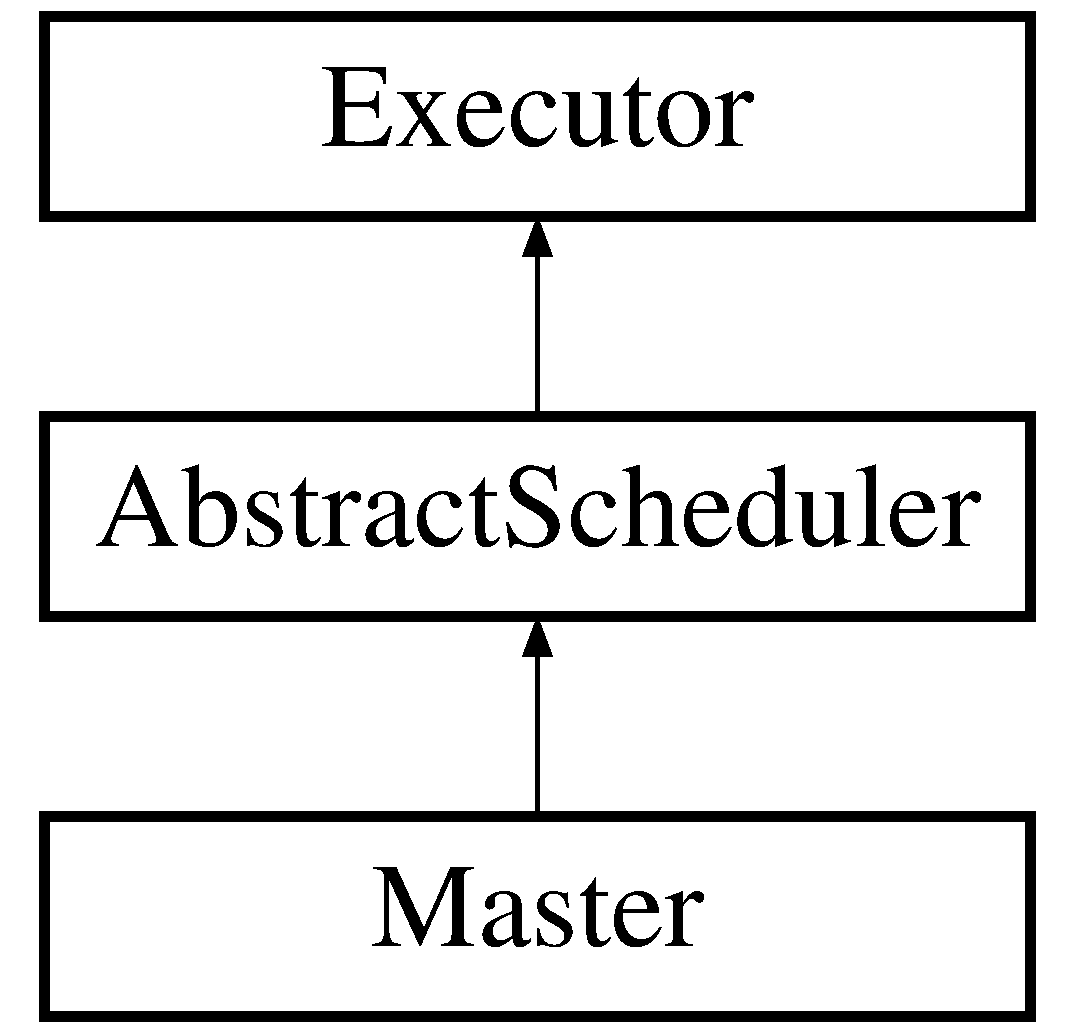
\includegraphics[height=3.000000cm]{class_master}
\end{center}
\end{figure}
\subsection*{Public Member Functions}
\begin{DoxyCompactItemize}
\item 
\hyperlink{class_master_a4ffd1a0c99fc39712ac89c50f87dedfa}{Master} (\hyperlink{class_scheduling_strategy}{Scheduling\+Strategy} $\ast$\hyperlink{class_abstract_scheduler_a7dd11eee79bfb44c820d6c28480fd0c7}{scheduling\+\_\+strategy}, \hyperlink{class_data_mining}{Data\+Mining} $\ast$\hyperlink{class_abstract_scheduler_a6e281d90fa4b965779cd13eabf7d0249}{data\+\_\+miner}, int \hyperlink{class_executor_a33c24e2887b4d9c4ef7f3566d3bc803e}{rank}, int \hyperlink{class_executor_a4e798bde66d26fe200de7e8d2b54e915}{number\+\_\+of\+\_\+processors})
\item 
\hyperlink{class_master_a20f70958ed75532ba672af1b780f59eb}{$\sim$\+Master} ()
\item 
void \hyperlink{class_master_acea94dce898273bbbddfaae52f243bca}{execute} (int argc, char $\ast$argv\mbox{[}$\,$\mbox{]})
\end{DoxyCompactItemize}
\subsection*{Additional Inherited Members}


\subsection{Detailed Description}
The \hyperlink{class_master}{Master} class inherits from the \hyperlink{class_abstract_scheduler}{Abstract\+Scheduler} class and implements the master-\/worker scheduling design. The \hyperlink{class_master}{Master} class collects scientific tasks and order them depending on the chosen scheduling strategy such as \hyperlink{class_f_i_f_o}{F\+I\+F\+O}, \hyperlink{class_l_i_f_o}{L\+I\+F\+O}, \hyperlink{class_s_j_f}{S\+J\+F} and \hyperlink{class_l_j_f}{L\+J\+F}. The class adds worker executor in a queue and sends them scientific tasks using the M\+P\+I\+\_\+\+Send() function and waits for receiving F\+I\+N\+I\+S\+H or R\+E\+Q\+U\+E\+S\+T tags using the M\+P\+I\+\_\+\+Recv() function. If the master receives a F\+I\+N\+I\+S\+H tag, the master will add the worker to the free\+\_\+worker queue. If the master receives a R\+E\+Q\+U\+E\+S\+T tag with a scientific task, the master will add the scientific task to the scheduling queue.

If the is\+\_\+finish() function returns true, the master will send a message using M\+P\+I\+\_\+\+Send() with the tag S\+T\+O\+P to all worker executors and database servers to terminate them.

\begin{DoxyAuthor}{Author}
Fabio Broghammer 
\end{DoxyAuthor}
\begin{DoxyVersion}{Version}
1.\+0 
\end{DoxyVersion}


Definition at line 23 of file Master.\+h.



\subsection{Constructor \& Destructor Documentation}
\hypertarget{class_master_a4ffd1a0c99fc39712ac89c50f87dedfa}{}\index{Master@{Master}!Master@{Master}}
\index{Master@{Master}!Master@{Master}}
\subsubsection[{Master}]{\setlength{\rightskip}{0pt plus 5cm}Master\+::\+Master (
\begin{DoxyParamCaption}
\item[{{\bf Scheduling\+Strategy} $\ast$}]{scheduling\+\_\+strategy, }
\item[{{\bf Data\+Mining} $\ast$}]{data\+\_\+miner, }
\item[{int}]{rank, }
\item[{int}]{number\+\_\+of\+\_\+processors}
\end{DoxyParamCaption}
)}\label{class_master_a4ffd1a0c99fc39712ac89c50f87dedfa}
Constructs a new master for master -\/ worker scheduling. The constructor only initialize the queue free\+\_\+worker and calls the super constructor


\begin{DoxyParams}{Parameters}
{\em scheduling\+\_\+strategy} & the scheduling strategy to be set \\
\hline
{\em data\+\_\+mining} & the data miner to be set \\
\hline
{\em rank} & the M\+P\+I rank of the processors, that execute the scheduler \\
\hline
{\em number\+\_\+of\+\_\+processors} & the total number of processors of the M\+P\+I world \\
\hline
\end{DoxyParams}


Definition at line 9 of file Master.\+cpp.

\hypertarget{class_master_a20f70958ed75532ba672af1b780f59eb}{}\index{Master@{Master}!````~Master@{$\sim$\+Master}}
\index{````~Master@{$\sim$\+Master}!Master@{Master}}
\subsubsection[{$\sim$\+Master}]{\setlength{\rightskip}{0pt plus 5cm}Master\+::$\sim$\+Master (
\begin{DoxyParamCaption}
{}
\end{DoxyParamCaption}
)}\label{class_master_a20f70958ed75532ba672af1b780f59eb}
Deletes the queue free\+\_\+worker object 

Definition at line 15 of file Master.\+cpp.



\subsection{Member Function Documentation}
\hypertarget{class_master_acea94dce898273bbbddfaae52f243bca}{}\index{Master@{Master}!execute@{execute}}
\index{execute@{execute}!Master@{Master}}
\subsubsection[{execute}]{\setlength{\rightskip}{0pt plus 5cm}void Master\+::execute (
\begin{DoxyParamCaption}
\item[{int}]{argc, }
\item[{char $\ast$}]{argv\mbox{[}$\,$\mbox{]}}
\end{DoxyParamCaption}
)\hspace{0.3cm}{\ttfamily [virtual]}}\label{class_master_acea94dce898273bbbddfaae52f243bca}
Override the execute function from executor. This function ist called to start the master


\begin{DoxyParams}{Parameters}
{\em argc} & command line argument count \\
\hline
{\em argv} & command line arguments \\
\hline
\end{DoxyParams}


Implements \hyperlink{class_executor_aabad4923751a6ea70ca536d4d1f2f32a}{Executor}.



Definition at line 70 of file Master.\+cpp.



The documentation for this class was generated from the following files\+:\begin{DoxyCompactItemize}
\item 
src/scheduler/\hyperlink{_master_8h}{Master.\+h}\item 
src/scheduler/\hyperlink{_master_8cpp}{Master.\+cpp}\end{DoxyCompactItemize}

\hypertarget{classel_1_1base_1_1_message_builder}{}\section{el\+:\+:base\+:\+:Message\+Builder Class Reference}
\label{classel_1_1base_1_1_message_builder}\index{el\+::base\+::\+Message\+Builder@{el\+::base\+::\+Message\+Builder}}


{\ttfamily \#include $<$easylogging++.\+h$>$}

\subsection*{Public Member Functions}
\begin{DoxyCompactItemize}
\item 
\hyperlink{classel_1_1base_1_1_message_builder_ac0b1b1be970ceab13eb023ef0399ef87}{Message\+Builder} (void)
\item 
void \hyperlink{classel_1_1base_1_1_message_builder_a61729d9b620eb7b3e6ac1af69364553c}{initialize} (\hyperlink{classel_1_1_logger}{Logger} $\ast$logger)
\item 
\hyperlink{classel_1_1base_1_1_message_builder}{Message\+Builder} \& \hyperlink{classel_1_1base_1_1_message_builder_a740a968d7f2901d49a2e1c348cfea7bf}{operator$<$$<$} (const std\+::string \&msg)
\item 
\hyperlink{classel_1_1base_1_1_message_builder}{Message\+Builder} \& \hyperlink{classel_1_1base_1_1_message_builder_ad04c5d0a8fc38662ede9aaa742912a42}{operator$<$$<$} (const std\+::wstring \&msg)
\item 
\hyperlink{classel_1_1base_1_1_message_builder}{Message\+Builder} \& \hyperlink{classel_1_1base_1_1_message_builder_a42c2a21a6bebb2ad52d22da054cd8f49}{operator$<$$<$} (const wchar\+\_\+t $\ast$msg)
\item 
\hyperlink{classel_1_1base_1_1_message_builder}{Message\+Builder} \& \hyperlink{classel_1_1base_1_1_message_builder_a884b9fd5f742f5fa25bbc78d3415a674}{operator$<$$<$} (std\+::ostream \&($\ast$O\+Stream\+Mani)(std\+::ostream \&))
\end{DoxyCompactItemize}


\subsection{Detailed Description}


Definition at line 4563 of file easylogging++.\+h.



\subsection{Constructor \& Destructor Documentation}
\hypertarget{classel_1_1base_1_1_message_builder_ac0b1b1be970ceab13eb023ef0399ef87}{}\index{el\+::base\+::\+Message\+Builder@{el\+::base\+::\+Message\+Builder}!Message\+Builder@{Message\+Builder}}
\index{Message\+Builder@{Message\+Builder}!el\+::base\+::\+Message\+Builder@{el\+::base\+::\+Message\+Builder}}
\subsubsection[{Message\+Builder}]{\setlength{\rightskip}{0pt plus 5cm}el\+::base\+::\+Message\+Builder\+::\+Message\+Builder (
\begin{DoxyParamCaption}
\item[{void}]{}
\end{DoxyParamCaption}
)\hspace{0.3cm}{\ttfamily [inline]}}\label{classel_1_1base_1_1_message_builder_ac0b1b1be970ceab13eb023ef0399ef87}


Definition at line 4565 of file easylogging++.\+h.



\subsection{Member Function Documentation}
\hypertarget{classel_1_1base_1_1_message_builder_a61729d9b620eb7b3e6ac1af69364553c}{}\index{el\+::base\+::\+Message\+Builder@{el\+::base\+::\+Message\+Builder}!initialize@{initialize}}
\index{initialize@{initialize}!el\+::base\+::\+Message\+Builder@{el\+::base\+::\+Message\+Builder}}
\subsubsection[{initialize}]{\setlength{\rightskip}{0pt plus 5cm}void el\+::base\+::\+Message\+Builder\+::initialize (
\begin{DoxyParamCaption}
\item[{{\bf Logger} $\ast$}]{logger}
\end{DoxyParamCaption}
)\hspace{0.3cm}{\ttfamily [inline]}}\label{classel_1_1base_1_1_message_builder_a61729d9b620eb7b3e6ac1af69364553c}


Definition at line 4566 of file easylogging++.\+h.

\hypertarget{classel_1_1base_1_1_message_builder_a740a968d7f2901d49a2e1c348cfea7bf}{}\index{el\+::base\+::\+Message\+Builder@{el\+::base\+::\+Message\+Builder}!operator$<$$<$@{operator$<$$<$}}
\index{operator$<$$<$@{operator$<$$<$}!el\+::base\+::\+Message\+Builder@{el\+::base\+::\+Message\+Builder}}
\subsubsection[{operator$<$$<$}]{\setlength{\rightskip}{0pt plus 5cm}{\bf Message\+Builder}\& el\+::base\+::\+Message\+Builder\+::operator$<$$<$ (
\begin{DoxyParamCaption}
\item[{const std\+::string \&}]{msg}
\end{DoxyParamCaption}
)\hspace{0.3cm}{\ttfamily [inline]}}\label{classel_1_1base_1_1_message_builder_a740a968d7f2901d49a2e1c348cfea7bf}


Definition at line 4581 of file easylogging++.\+h.

\hypertarget{classel_1_1base_1_1_message_builder_ad04c5d0a8fc38662ede9aaa742912a42}{}\index{el\+::base\+::\+Message\+Builder@{el\+::base\+::\+Message\+Builder}!operator$<$$<$@{operator$<$$<$}}
\index{operator$<$$<$@{operator$<$$<$}!el\+::base\+::\+Message\+Builder@{el\+::base\+::\+Message\+Builder}}
\subsubsection[{operator$<$$<$}]{\setlength{\rightskip}{0pt plus 5cm}{\bf Message\+Builder}\& el\+::base\+::\+Message\+Builder\+::operator$<$$<$ (
\begin{DoxyParamCaption}
\item[{const std\+::wstring \&}]{msg}
\end{DoxyParamCaption}
)\hspace{0.3cm}{\ttfamily [inline]}}\label{classel_1_1base_1_1_message_builder_ad04c5d0a8fc38662ede9aaa742912a42}


Definition at line 4598 of file easylogging++.\+h.

\hypertarget{classel_1_1base_1_1_message_builder_a42c2a21a6bebb2ad52d22da054cd8f49}{}\index{el\+::base\+::\+Message\+Builder@{el\+::base\+::\+Message\+Builder}!operator$<$$<$@{operator$<$$<$}}
\index{operator$<$$<$@{operator$<$$<$}!el\+::base\+::\+Message\+Builder@{el\+::base\+::\+Message\+Builder}}
\subsubsection[{operator$<$$<$}]{\setlength{\rightskip}{0pt plus 5cm}{\bf Message\+Builder}\& el\+::base\+::\+Message\+Builder\+::operator$<$$<$ (
\begin{DoxyParamCaption}
\item[{const wchar\+\_\+t $\ast$}]{msg}
\end{DoxyParamCaption}
)\hspace{0.3cm}{\ttfamily [inline]}}\label{classel_1_1base_1_1_message_builder_a42c2a21a6bebb2ad52d22da054cd8f49}


Definition at line 4601 of file easylogging++.\+h.

\hypertarget{classel_1_1base_1_1_message_builder_a884b9fd5f742f5fa25bbc78d3415a674}{}\index{el\+::base\+::\+Message\+Builder@{el\+::base\+::\+Message\+Builder}!operator$<$$<$@{operator$<$$<$}}
\index{operator$<$$<$@{operator$<$$<$}!el\+::base\+::\+Message\+Builder@{el\+::base\+::\+Message\+Builder}}
\subsubsection[{operator$<$$<$}]{\setlength{\rightskip}{0pt plus 5cm}{\bf Message\+Builder}\& el\+::base\+::\+Message\+Builder\+::operator$<$$<$ (
\begin{DoxyParamCaption}
\item[{std\+::ostream \&($\ast$)(std\+::ostream \&)}]{O\+Stream\+Mani}
\end{DoxyParamCaption}
)\hspace{0.3cm}{\ttfamily [inline]}}\label{classel_1_1base_1_1_message_builder_a884b9fd5f742f5fa25bbc78d3415a674}


Definition at line 4619 of file easylogging++.\+h.



The documentation for this class was generated from the following file\+:\begin{DoxyCompactItemize}
\item 
lib/\hyperlink{easylogging_09_09_8h}{easylogging++.\+h}\end{DoxyCompactItemize}

\hypertarget{classel_1_1base_1_1_milliseconds_width}{}\section{el\+:\+:base\+:\+:Milliseconds\+Width Class Reference}
\label{classel_1_1base_1_1_milliseconds_width}\index{el\+::base\+::\+Milliseconds\+Width@{el\+::base\+::\+Milliseconds\+Width}}


A milliseconds width class containing actual width and offset for date/time.  




{\ttfamily \#include $<$easylogging++.\+h$>$}

\subsection*{Public Member Functions}
\begin{DoxyCompactItemize}
\item 
\hyperlink{classel_1_1base_1_1_milliseconds_width_a87712d779ce80d6ba4fffb3b7d20d1bd}{Milliseconds\+Width} (void)
\item 
\hyperlink{classel_1_1base_1_1_milliseconds_width_a358fa0fcdd4076c4038ecdfc206de38a}{Milliseconds\+Width} (int width)
\item 
bool \hyperlink{classel_1_1base_1_1_milliseconds_width_a60f5fb6e31216d1268585b98d20517ff}{operator==} (const \hyperlink{classel_1_1base_1_1_milliseconds_width}{Milliseconds\+Width} \&ms\+Width)
\end{DoxyCompactItemize}
\subsection*{Public Attributes}
\begin{DoxyCompactItemize}
\item 
int \hyperlink{classel_1_1base_1_1_milliseconds_width_a31c468b0323d376505c4975720c7b66e}{m\+\_\+width}
\item 
unsigned int \hyperlink{classel_1_1base_1_1_milliseconds_width_a0e98edbecf602a915d4d609747c52669}{m\+\_\+offset}
\end{DoxyCompactItemize}


\subsection{Detailed Description}
A milliseconds width class containing actual width and offset for date/time. 

Definition at line 860 of file easylogging++.\+h.



\subsection{Constructor \& Destructor Documentation}
\hypertarget{classel_1_1base_1_1_milliseconds_width_a87712d779ce80d6ba4fffb3b7d20d1bd}{}\index{el\+::base\+::\+Milliseconds\+Width@{el\+::base\+::\+Milliseconds\+Width}!Milliseconds\+Width@{Milliseconds\+Width}}
\index{Milliseconds\+Width@{Milliseconds\+Width}!el\+::base\+::\+Milliseconds\+Width@{el\+::base\+::\+Milliseconds\+Width}}
\subsubsection[{Milliseconds\+Width}]{\setlength{\rightskip}{0pt plus 5cm}el\+::base\+::\+Milliseconds\+Width\+::\+Milliseconds\+Width (
\begin{DoxyParamCaption}
\item[{void}]{}
\end{DoxyParamCaption}
)\hspace{0.3cm}{\ttfamily [inline]}}\label{classel_1_1base_1_1_milliseconds_width_a87712d779ce80d6ba4fffb3b7d20d1bd}


Definition at line 862 of file easylogging++.\+h.

\hypertarget{classel_1_1base_1_1_milliseconds_width_a358fa0fcdd4076c4038ecdfc206de38a}{}\index{el\+::base\+::\+Milliseconds\+Width@{el\+::base\+::\+Milliseconds\+Width}!Milliseconds\+Width@{Milliseconds\+Width}}
\index{Milliseconds\+Width@{Milliseconds\+Width}!el\+::base\+::\+Milliseconds\+Width@{el\+::base\+::\+Milliseconds\+Width}}
\subsubsection[{Milliseconds\+Width}]{\setlength{\rightskip}{0pt plus 5cm}el\+::base\+::\+Milliseconds\+Width\+::\+Milliseconds\+Width (
\begin{DoxyParamCaption}
\item[{int}]{width}
\end{DoxyParamCaption}
)\hspace{0.3cm}{\ttfamily [inline]}, {\ttfamily [explicit]}}\label{classel_1_1base_1_1_milliseconds_width_a358fa0fcdd4076c4038ecdfc206de38a}


Definition at line 863 of file easylogging++.\+h.



\subsection{Member Function Documentation}
\hypertarget{classel_1_1base_1_1_milliseconds_width_a60f5fb6e31216d1268585b98d20517ff}{}\index{el\+::base\+::\+Milliseconds\+Width@{el\+::base\+::\+Milliseconds\+Width}!operator==@{operator==}}
\index{operator==@{operator==}!el\+::base\+::\+Milliseconds\+Width@{el\+::base\+::\+Milliseconds\+Width}}
\subsubsection[{operator==}]{\setlength{\rightskip}{0pt plus 5cm}bool el\+::base\+::\+Milliseconds\+Width\+::operator== (
\begin{DoxyParamCaption}
\item[{const {\bf Milliseconds\+Width} \&}]{ms\+Width}
\end{DoxyParamCaption}
)\hspace{0.3cm}{\ttfamily [inline]}}\label{classel_1_1base_1_1_milliseconds_width_a60f5fb6e31216d1268585b98d20517ff}


Definition at line 864 of file easylogging++.\+h.



\subsection{Member Data Documentation}
\hypertarget{classel_1_1base_1_1_milliseconds_width_a0e98edbecf602a915d4d609747c52669}{}\index{el\+::base\+::\+Milliseconds\+Width@{el\+::base\+::\+Milliseconds\+Width}!m\+\_\+offset@{m\+\_\+offset}}
\index{m\+\_\+offset@{m\+\_\+offset}!el\+::base\+::\+Milliseconds\+Width@{el\+::base\+::\+Milliseconds\+Width}}
\subsubsection[{m\+\_\+offset}]{\setlength{\rightskip}{0pt plus 5cm}unsigned int el\+::base\+::\+Milliseconds\+Width\+::m\+\_\+offset}\label{classel_1_1base_1_1_milliseconds_width_a0e98edbecf602a915d4d609747c52669}


Definition at line 865 of file easylogging++.\+h.

\hypertarget{classel_1_1base_1_1_milliseconds_width_a31c468b0323d376505c4975720c7b66e}{}\index{el\+::base\+::\+Milliseconds\+Width@{el\+::base\+::\+Milliseconds\+Width}!m\+\_\+width@{m\+\_\+width}}
\index{m\+\_\+width@{m\+\_\+width}!el\+::base\+::\+Milliseconds\+Width@{el\+::base\+::\+Milliseconds\+Width}}
\subsubsection[{m\+\_\+width}]{\setlength{\rightskip}{0pt plus 5cm}int el\+::base\+::\+Milliseconds\+Width\+::m\+\_\+width}\label{classel_1_1base_1_1_milliseconds_width_a31c468b0323d376505c4975720c7b66e}


Definition at line 865 of file easylogging++.\+h.



The documentation for this class was generated from the following file\+:\begin{DoxyCompactItemize}
\item 
lib/\hyperlink{easylogging_09_09_8h}{easylogging++.\+h}\end{DoxyCompactItemize}

\hypertarget{class_mpi_win_f_i_f_o}{}\section{Mpi\+Win\+F\+I\+F\+O Class Reference}
\label{class_mpi_win_f_i_f_o}\index{Mpi\+Win\+F\+I\+F\+O@{Mpi\+Win\+F\+I\+F\+O}}


{\ttfamily \#include $<$Mpi\+Win\+F\+I\+F\+O.\+h$>$}

Inheritance diagram for Mpi\+Win\+F\+I\+F\+O\+:\begin{figure}[H]
\begin{center}
\leavevmode
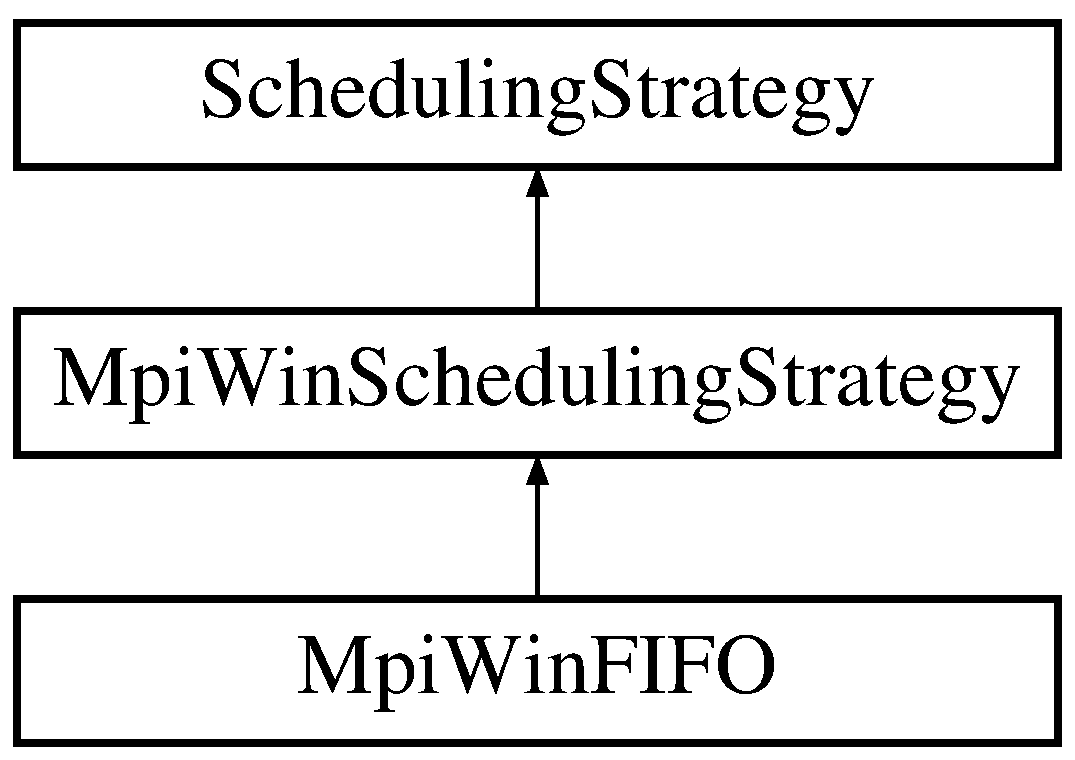
\includegraphics[height=3.000000cm]{class_mpi_win_f_i_f_o}
\end{center}
\end{figure}
\subsection*{Public Member Functions}
\begin{DoxyCompactItemize}
\item 
\hyperlink{class_mpi_win_f_i_f_o_a52b5238edee8c348afbf0d370c81d8ce}{Mpi\+Win\+F\+I\+F\+O} (int size, int rank, int number\+\_\+of\+\_\+processors)
\item 
\hyperlink{class_mpi_win_f_i_f_o_a6ca0a6e127618d262ae40d3171bbb672}{$\sim$\+Mpi\+Win\+F\+I\+F\+O} ()
\item 
\hyperlink{_types_8h_a0c77930ab3818a1680c59353f627fba8}{Task} \hyperlink{class_mpi_win_f_i_f_o_aeffee53a08818badfafed7642a41b955}{get\+\_\+next\+\_\+task} ()
\item 
int \hyperlink{class_mpi_win_f_i_f_o_a609d1de2a9afc8d82dfab9746fe7c885}{get\+\_\+task\+\_\+count} ()
\item 
\hyperlink{_types_8h_a0c77930ab3818a1680c59353f627fba8}{Task} \hyperlink{class_mpi_win_f_i_f_o_a1ceb2f48f1ae2fbbf14ab9227ba8df9e}{pop\+\_\+next\+\_\+task} ()
\item 
void \hyperlink{class_mpi_win_f_i_f_o_ab250777bda97e37530c354683a87e8b4}{push\+\_\+new\+\_\+task} (\hyperlink{_types_8h_a0c77930ab3818a1680c59353f627fba8}{Task} task, long runtime)
\item 
\hyperlink{class_scheduling_strategy}{Scheduling\+Strategy} $\ast$ \hyperlink{class_mpi_win_f_i_f_o_ae5620542c597abff58986506d595c29e}{change\+\_\+strategy} (\hyperlink{class_scheduling_strategy}{Scheduling\+Strategy} $\ast$new\+\_\+strategy)
\item 
\hyperlink{_types_8h_a0c77930ab3818a1680c59353f627fba8}{Task} \hyperlink{class_mpi_win_f_i_f_o_a8f4af1f3c3f90b939f3638bf321be3bf}{steal\+\_\+next\+\_\+task} (int target\+\_\+rank, int number\+\_\+of\+\_\+tries)
\item 
int \hyperlink{class_mpi_win_f_i_f_o_a7481a465167e95e3993251106fe40cb3}{get\+\_\+task\+\_\+count} (int target\+\_\+rank)
\item 
bool \hyperlink{class_mpi_win_f_i_f_o_ab568b8ec6f8eb9baabaae8552a938204}{is\+\_\+statistic\+\_\+based} ()
\end{DoxyCompactItemize}
\subsection*{Additional Inherited Members}


\subsection{Detailed Description}
This class implements the \hyperlink{class_mpi_win_scheduling_strategy}{Mpi\+Win\+Scheduling\+Strategy} and realize a \hyperlink{class_f_i_f_o}{F\+I\+F\+O} queue. The \hyperlink{class_f_i_f_o}{F\+I\+F\+O} queue is represented as cyclic array. (See \href{https://crypto.iti.kit.edu/fileadmin/User/Lectures/Algorithmen_SS15/folien_20150427.pdf}{\tt https\+://crypto.\+iti.\+kit.\+edu/fileadmin/\+User/\+Lectures/\+Algorithmen\+\_\+\+S\+S15/folien\+\_\+20150427.\+pdf} page 125) The queue itself and the offset are inside several M\+P\+I window to give other processes access to the data.

\begin{DoxyAuthor}{Author}
Fabio Broghammer 
\end{DoxyAuthor}
\begin{DoxyVersion}{Version}
1.\+0 
\end{DoxyVersion}


Definition at line 14 of file Mpi\+Win\+F\+I\+F\+O.\+h.



\subsection{Constructor \& Destructor Documentation}
\hypertarget{class_mpi_win_f_i_f_o_a52b5238edee8c348afbf0d370c81d8ce}{}\index{Mpi\+Win\+F\+I\+F\+O@{Mpi\+Win\+F\+I\+F\+O}!Mpi\+Win\+F\+I\+F\+O@{Mpi\+Win\+F\+I\+F\+O}}
\index{Mpi\+Win\+F\+I\+F\+O@{Mpi\+Win\+F\+I\+F\+O}!Mpi\+Win\+F\+I\+F\+O@{Mpi\+Win\+F\+I\+F\+O}}
\subsubsection[{Mpi\+Win\+F\+I\+F\+O}]{\setlength{\rightskip}{0pt plus 5cm}Mpi\+Win\+F\+I\+F\+O\+::\+Mpi\+Win\+F\+I\+F\+O (
\begin{DoxyParamCaption}
\item[{int}]{size, }
\item[{int}]{rank, }
\item[{int}]{number\+\_\+of\+\_\+processors}
\end{DoxyParamCaption}
)}\label{class_mpi_win_f_i_f_o_a52b5238edee8c348afbf0d370c81d8ce}
Constructs a new \hyperlink{class_l_i_f_o}{L\+I\+F\+O} scheduling queue


\begin{DoxyParams}{Parameters}
{\em size} & of the queue \\
\hline
{\em rank} & from the process inside the M\+Y\+\_\+\+M\+P\+I\+\_\+\+C\+O\+M\+M\+\_\+\+T\+A\+S\+K\+S\+T\+E\+A\+L\+I\+N\+G communicator \\
\hline
{\em number\+\_\+of\+\_\+processors} & inside the M\+Y\+\_\+\+M\+P\+I\+\_\+\+C\+O\+M\+M\+\_\+\+T\+A\+S\+K\+S\+T\+E\+A\+L\+I\+N\+G communicator \\
\hline
\end{DoxyParams}


Definition at line 6 of file Mpi\+Win\+F\+I\+F\+O.\+cpp.

\hypertarget{class_mpi_win_f_i_f_o_a6ca0a6e127618d262ae40d3171bbb672}{}\index{Mpi\+Win\+F\+I\+F\+O@{Mpi\+Win\+F\+I\+F\+O}!````~Mpi\+Win\+F\+I\+F\+O@{$\sim$\+Mpi\+Win\+F\+I\+F\+O}}
\index{````~Mpi\+Win\+F\+I\+F\+O@{$\sim$\+Mpi\+Win\+F\+I\+F\+O}!Mpi\+Win\+F\+I\+F\+O@{Mpi\+Win\+F\+I\+F\+O}}
\subsubsection[{$\sim$\+Mpi\+Win\+F\+I\+F\+O}]{\setlength{\rightskip}{0pt plus 5cm}Mpi\+Win\+F\+I\+F\+O\+::$\sim$\+Mpi\+Win\+F\+I\+F\+O (
\begin{DoxyParamCaption}
{}
\end{DoxyParamCaption}
)}\label{class_mpi_win_f_i_f_o_a6ca0a6e127618d262ae40d3171bbb672}
Destructs a new \hyperlink{class_l_i_f_o}{L\+I\+F\+O} scheduling queue 

Definition at line 14 of file Mpi\+Win\+F\+I\+F\+O.\+cpp.



\subsection{Member Function Documentation}
\hypertarget{class_mpi_win_f_i_f_o_ae5620542c597abff58986506d595c29e}{}\index{Mpi\+Win\+F\+I\+F\+O@{Mpi\+Win\+F\+I\+F\+O}!change\+\_\+strategy@{change\+\_\+strategy}}
\index{change\+\_\+strategy@{change\+\_\+strategy}!Mpi\+Win\+F\+I\+F\+O@{Mpi\+Win\+F\+I\+F\+O}}
\subsubsection[{change\+\_\+strategy}]{\setlength{\rightskip}{0pt plus 5cm}{\bf Scheduling\+Strategy} $\ast$ Mpi\+Win\+F\+I\+F\+O\+::change\+\_\+strategy (
\begin{DoxyParamCaption}
\item[{{\bf Scheduling\+Strategy} $\ast$}]{new\+\_\+strategy}
\end{DoxyParamCaption}
)\hspace{0.3cm}{\ttfamily [virtual]}}\label{class_mpi_win_f_i_f_o_ae5620542c597abff58986506d595c29e}
Changes the scheduling strategy. Returns the new scheduling strategy with all tasks, or N\+U\+L\+L if there was an error.

Estimated runtime of tasks will get lost by changing from statistically based strategies (L\+S\+F, \hyperlink{class_s_j_f}{S\+J\+F}) to non-\/statistically based strategies. The order of the old queue will be kept.

All tasks will get a default runtime value (defined in D\+E\+F\+A\+U\+L\+T\+\_\+\+R\+U\+N\+T\+I\+M\+E) by changing from non-\/statistically based strategies (\hyperlink{class_f_i_f_o}{F\+I\+F\+O}, \hyperlink{class_l_i_f_o}{L\+I\+F\+O}) to statistically based strategies. The order of the old queue perhaps won\textquotesingle{}t be kept 
\begin{DoxyParams}{Parameters}
{\em new\+\_\+strategy} & \\
\hline
\end{DoxyParams}


Implements \hyperlink{class_scheduling_strategy_a4874d194c1bb185480339360fe907d83}{Scheduling\+Strategy}.



Definition at line 95 of file Mpi\+Win\+F\+I\+F\+O.\+cpp.

\hypertarget{class_mpi_win_f_i_f_o_aeffee53a08818badfafed7642a41b955}{}\index{Mpi\+Win\+F\+I\+F\+O@{Mpi\+Win\+F\+I\+F\+O}!get\+\_\+next\+\_\+task@{get\+\_\+next\+\_\+task}}
\index{get\+\_\+next\+\_\+task@{get\+\_\+next\+\_\+task}!Mpi\+Win\+F\+I\+F\+O@{Mpi\+Win\+F\+I\+F\+O}}
\subsubsection[{get\+\_\+next\+\_\+task}]{\setlength{\rightskip}{0pt plus 5cm}{\bf Task} Mpi\+Win\+F\+I\+F\+O\+::get\+\_\+next\+\_\+task (
\begin{DoxyParamCaption}
{}
\end{DoxyParamCaption}
)\hspace{0.3cm}{\ttfamily [virtual]}}\label{class_mpi_win_f_i_f_o_aeffee53a08818badfafed7642a41b955}
Returns the last-\/in task, or N\+U\+L\+L if the queue is empty

\begin{DoxyReturn}{Returns}
the last-\/in task 
\end{DoxyReturn}


Implements \hyperlink{class_scheduling_strategy_adce3619801460ad67d6c8f9bdffcd36b}{Scheduling\+Strategy}.



Definition at line 39 of file Mpi\+Win\+F\+I\+F\+O.\+cpp.

\hypertarget{class_mpi_win_f_i_f_o_a609d1de2a9afc8d82dfab9746fe7c885}{}\index{Mpi\+Win\+F\+I\+F\+O@{Mpi\+Win\+F\+I\+F\+O}!get\+\_\+task\+\_\+count@{get\+\_\+task\+\_\+count}}
\index{get\+\_\+task\+\_\+count@{get\+\_\+task\+\_\+count}!Mpi\+Win\+F\+I\+F\+O@{Mpi\+Win\+F\+I\+F\+O}}
\subsubsection[{get\+\_\+task\+\_\+count}]{\setlength{\rightskip}{0pt plus 5cm}int Mpi\+Win\+F\+I\+F\+O\+::get\+\_\+task\+\_\+count (
\begin{DoxyParamCaption}
{}
\end{DoxyParamCaption}
)\hspace{0.3cm}{\ttfamily [virtual]}}\label{class_mpi_win_f_i_f_o_a609d1de2a9afc8d82dfab9746fe7c885}
Return the count of tasks in the scheduling queue

\begin{DoxyReturn}{Returns}
the count of tasks 
\end{DoxyReturn}


Implements \hyperlink{class_scheduling_strategy_a0a3355ffe9c03236692ad00e4f94f5c5}{Scheduling\+Strategy}.



Definition at line 99 of file Mpi\+Win\+F\+I\+F\+O.\+cpp.

\hypertarget{class_mpi_win_f_i_f_o_a7481a465167e95e3993251106fe40cb3}{}\index{Mpi\+Win\+F\+I\+F\+O@{Mpi\+Win\+F\+I\+F\+O}!get\+\_\+task\+\_\+count@{get\+\_\+task\+\_\+count}}
\index{get\+\_\+task\+\_\+count@{get\+\_\+task\+\_\+count}!Mpi\+Win\+F\+I\+F\+O@{Mpi\+Win\+F\+I\+F\+O}}
\subsubsection[{get\+\_\+task\+\_\+count}]{\setlength{\rightskip}{0pt plus 5cm}int Mpi\+Win\+F\+I\+F\+O\+::get\+\_\+task\+\_\+count (
\begin{DoxyParamCaption}
\item[{int}]{target\+\_\+rank}
\end{DoxyParamCaption}
)\hspace{0.3cm}{\ttfamily [virtual]}}\label{class_mpi_win_f_i_f_o_a7481a465167e95e3993251106fe40cb3}
Returns the task count of the remote queue of the given rank


\begin{DoxyParams}{Parameters}
{\em rank} & the rank of the remote queue\\
\hline
\end{DoxyParams}
\begin{DoxyReturn}{Returns}
the task count of the remote queue 
\end{DoxyReturn}


Implements \hyperlink{class_mpi_win_scheduling_strategy_a8742d0d3a2204efe5aa47e39f856dee1}{Mpi\+Win\+Scheduling\+Strategy}.



Definition at line 104 of file Mpi\+Win\+F\+I\+F\+O.\+cpp.

\hypertarget{class_mpi_win_f_i_f_o_ab568b8ec6f8eb9baabaae8552a938204}{}\index{Mpi\+Win\+F\+I\+F\+O@{Mpi\+Win\+F\+I\+F\+O}!is\+\_\+statistic\+\_\+based@{is\+\_\+statistic\+\_\+based}}
\index{is\+\_\+statistic\+\_\+based@{is\+\_\+statistic\+\_\+based}!Mpi\+Win\+F\+I\+F\+O@{Mpi\+Win\+F\+I\+F\+O}}
\subsubsection[{is\+\_\+statistic\+\_\+based}]{\setlength{\rightskip}{0pt plus 5cm}bool Mpi\+Win\+F\+I\+F\+O\+::is\+\_\+statistic\+\_\+based (
\begin{DoxyParamCaption}
{}
\end{DoxyParamCaption}
)\hspace{0.3cm}{\ttfamily [virtual]}}\label{class_mpi_win_f_i_f_o_ab568b8ec6f8eb9baabaae8552a938204}
Returns true, if the current scheduling strategy statistic based.

\begin{DoxyReturn}{Returns}
true, if the current scheduling strategy statistic based 
\end{DoxyReturn}


Implements \hyperlink{class_scheduling_strategy_a5962845ca5af53bbdc014c19a6bdef99}{Scheduling\+Strategy}.



Definition at line 115 of file Mpi\+Win\+F\+I\+F\+O.\+cpp.

\hypertarget{class_mpi_win_f_i_f_o_a1ceb2f48f1ae2fbbf14ab9227ba8df9e}{}\index{Mpi\+Win\+F\+I\+F\+O@{Mpi\+Win\+F\+I\+F\+O}!pop\+\_\+next\+\_\+task@{pop\+\_\+next\+\_\+task}}
\index{pop\+\_\+next\+\_\+task@{pop\+\_\+next\+\_\+task}!Mpi\+Win\+F\+I\+F\+O@{Mpi\+Win\+F\+I\+F\+O}}
\subsubsection[{pop\+\_\+next\+\_\+task}]{\setlength{\rightskip}{0pt plus 5cm}{\bf Task} Mpi\+Win\+F\+I\+F\+O\+::pop\+\_\+next\+\_\+task (
\begin{DoxyParamCaption}
{}
\end{DoxyParamCaption}
)\hspace{0.3cm}{\ttfamily [virtual]}}\label{class_mpi_win_f_i_f_o_a1ceb2f48f1ae2fbbf14ab9227ba8df9e}
Removes the next task in the queue, effectively reducing its size by one. 

Implements \hyperlink{class_scheduling_strategy_ac2ba483287c91fd4318f337da144a9c5}{Scheduling\+Strategy}.



Definition at line 44 of file Mpi\+Win\+F\+I\+F\+O.\+cpp.

\hypertarget{class_mpi_win_f_i_f_o_ab250777bda97e37530c354683a87e8b4}{}\index{Mpi\+Win\+F\+I\+F\+O@{Mpi\+Win\+F\+I\+F\+O}!push\+\_\+new\+\_\+task@{push\+\_\+new\+\_\+task}}
\index{push\+\_\+new\+\_\+task@{push\+\_\+new\+\_\+task}!Mpi\+Win\+F\+I\+F\+O@{Mpi\+Win\+F\+I\+F\+O}}
\subsubsection[{push\+\_\+new\+\_\+task}]{\setlength{\rightskip}{0pt plus 5cm}void Mpi\+Win\+F\+I\+F\+O\+::push\+\_\+new\+\_\+task (
\begin{DoxyParamCaption}
\item[{{\bf Task}}]{task, }
\item[{long}]{runtime}
\end{DoxyParamCaption}
)\hspace{0.3cm}{\ttfamily [virtual]}}\label{class_mpi_win_f_i_f_o_ab250777bda97e37530c354683a87e8b4}
Insert a new task in the scheduling queue depending on the scheduling strategy and the estimated runtime 
\begin{DoxyParams}{Parameters}
{\em task} & \\
\hline
{\em runtime} & \\
\hline
\end{DoxyParams}


Implements \hyperlink{class_scheduling_strategy_a62ffa0426528c14fdd0b0853f04a851f}{Scheduling\+Strategy}.



Definition at line 58 of file Mpi\+Win\+F\+I\+F\+O.\+cpp.

\hypertarget{class_mpi_win_f_i_f_o_a8f4af1f3c3f90b939f3638bf321be3bf}{}\index{Mpi\+Win\+F\+I\+F\+O@{Mpi\+Win\+F\+I\+F\+O}!steal\+\_\+next\+\_\+task@{steal\+\_\+next\+\_\+task}}
\index{steal\+\_\+next\+\_\+task@{steal\+\_\+next\+\_\+task}!Mpi\+Win\+F\+I\+F\+O@{Mpi\+Win\+F\+I\+F\+O}}
\subsubsection[{steal\+\_\+next\+\_\+task}]{\setlength{\rightskip}{0pt plus 5cm}{\bf Task} Mpi\+Win\+F\+I\+F\+O\+::steal\+\_\+next\+\_\+task (
\begin{DoxyParamCaption}
\item[{int}]{target\+\_\+rank, }
\item[{int}]{number\+\_\+of\+\_\+tries}
\end{DoxyParamCaption}
)\hspace{0.3cm}{\ttfamily [virtual]}}\label{class_mpi_win_f_i_f_o_a8f4af1f3c3f90b939f3638bf321be3bf}
Steals the next task from the given rank if the queue of the given rank is not empty


\begin{DoxyParams}{Parameters}
{\em rank} & the rank of the remote queue\\
\hline
\end{DoxyParams}
\begin{DoxyReturn}{Returns}
the next task from the given rank or N\+U\+L\+L if the queue is empty 
\end{DoxyReturn}


Implements \hyperlink{class_mpi_win_scheduling_strategy_ac1804574e61c9ed91c7f78bc48b332ea}{Mpi\+Win\+Scheduling\+Strategy}.



Definition at line 120 of file Mpi\+Win\+F\+I\+F\+O.\+cpp.



The documentation for this class was generated from the following files\+:\begin{DoxyCompactItemize}
\item 
src/scheduler/\hyperlink{_mpi_win_f_i_f_o_8h}{Mpi\+Win\+F\+I\+F\+O.\+h}\item 
src/scheduler/\hyperlink{_mpi_win_f_i_f_o_8cpp}{Mpi\+Win\+F\+I\+F\+O.\+cpp}\end{DoxyCompactItemize}

\hypertarget{class_mpi_win_l_i_f_o}{}\section{Mpi\+Win\+L\+I\+F\+O Class Reference}
\label{class_mpi_win_l_i_f_o}\index{Mpi\+Win\+L\+I\+F\+O@{Mpi\+Win\+L\+I\+F\+O}}


{\ttfamily \#include $<$Mpi\+Win\+L\+I\+F\+O.\+h$>$}

Inheritance diagram for Mpi\+Win\+L\+I\+F\+O\+:\begin{figure}[H]
\begin{center}
\leavevmode
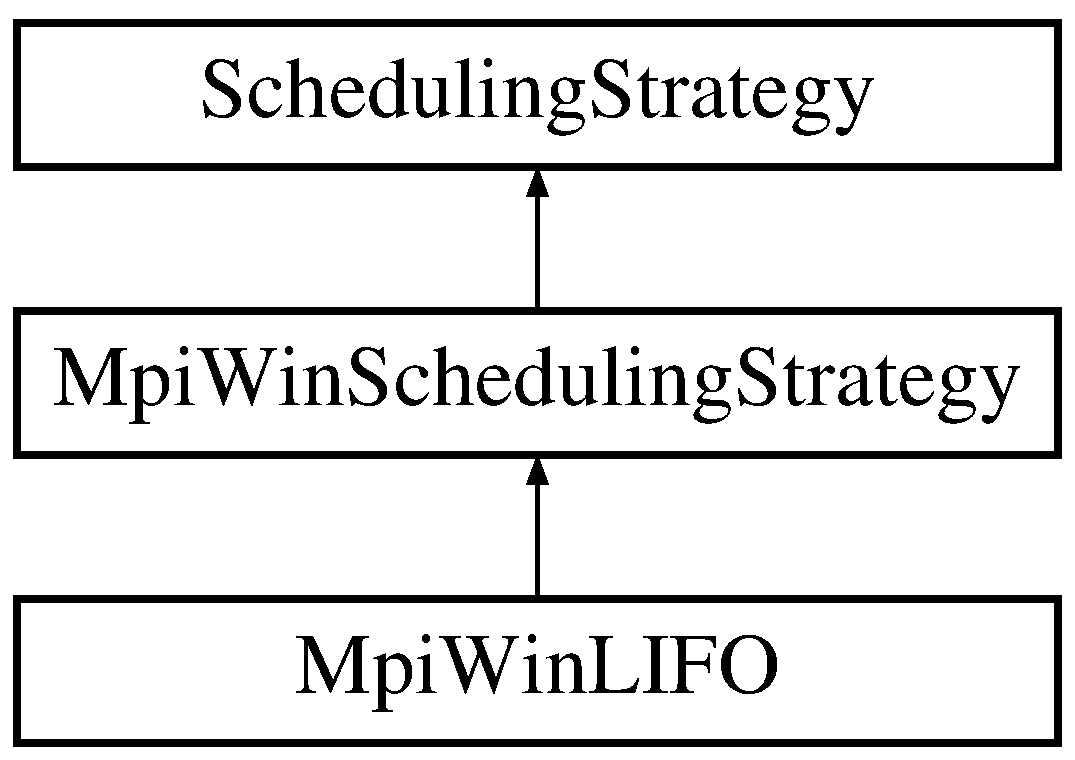
\includegraphics[height=3.000000cm]{class_mpi_win_l_i_f_o}
\end{center}
\end{figure}
\subsection*{Public Member Functions}
\begin{DoxyCompactItemize}
\item 
\hyperlink{class_mpi_win_l_i_f_o_a46a7cbb4d81782b9ff7dbd971e5eb9ca}{Mpi\+Win\+L\+I\+F\+O} (int size, int rank, int number\+\_\+of\+\_\+processors)
\item 
\hyperlink{class_mpi_win_l_i_f_o_a39fbceec3a4fb97990a31ff556ce8ff5}{$\sim$\+Mpi\+Win\+L\+I\+F\+O} ()
\item 
\hyperlink{_types_8h_a0c77930ab3818a1680c59353f627fba8}{Task} \hyperlink{class_mpi_win_l_i_f_o_a6de2bf8f36458582ebc800f2beda94c6}{get\+\_\+next\+\_\+task} ()
\item 
int \hyperlink{class_mpi_win_l_i_f_o_aeb679863632de7367029fded90eb4e5f}{get\+\_\+task\+\_\+count} ()
\item 
\hyperlink{_types_8h_a0c77930ab3818a1680c59353f627fba8}{Task} \hyperlink{class_mpi_win_l_i_f_o_a93c2fdd8d75ce1264329edfa48d8864a}{pop\+\_\+next\+\_\+task} ()
\item 
void \hyperlink{class_mpi_win_l_i_f_o_a1336e4abb196dc1f3eba6e7e29f969aa}{push\+\_\+new\+\_\+task} (\hyperlink{_types_8h_a0c77930ab3818a1680c59353f627fba8}{Task} task, long runtime)
\item 
\hyperlink{class_scheduling_strategy}{Scheduling\+Strategy} $\ast$ \hyperlink{class_mpi_win_l_i_f_o_aa33f53bcf71ee26ff20039916cb321cd}{change\+\_\+strategy} (\hyperlink{class_scheduling_strategy}{Scheduling\+Strategy} $\ast$new\+\_\+strategy)
\item 
\hyperlink{_types_8h_a0c77930ab3818a1680c59353f627fba8}{Task} \hyperlink{class_mpi_win_l_i_f_o_a0631b1fc2042f19a5b438c8cfa44934a}{steal\+\_\+next\+\_\+task} (int target\+\_\+rank, int number\+\_\+of\+\_\+tries)
\item 
int \hyperlink{class_mpi_win_l_i_f_o_a4825ff8faf740b1f9e984813c20455ec}{get\+\_\+task\+\_\+count} (int target\+\_\+rank)
\item 
bool \hyperlink{class_mpi_win_l_i_f_o_ae65b1f7b9a7e5c8a2feaceafca0dd129}{is\+\_\+statistic\+\_\+based} ()
\end{DoxyCompactItemize}
\subsection*{Additional Inherited Members}


\subsection{Detailed Description}
This class implements the \hyperlink{class_mpi_win_scheduling_strategy}{Mpi\+Win\+Scheduling\+Strategy} and realize a \hyperlink{class_l_i_f_o}{L\+I\+F\+O} queue. The queue itself and the offset are inside several M\+P\+I window to give other processes access to the data.

\begin{DoxyAuthor}{Author}
Fabio Broghammer 
\end{DoxyAuthor}
\begin{DoxyVersion}{Version}
1.\+0 
\end{DoxyVersion}


Definition at line 18 of file Mpi\+Win\+L\+I\+F\+O.\+h.



\subsection{Constructor \& Destructor Documentation}
\hypertarget{class_mpi_win_l_i_f_o_a46a7cbb4d81782b9ff7dbd971e5eb9ca}{}\index{Mpi\+Win\+L\+I\+F\+O@{Mpi\+Win\+L\+I\+F\+O}!Mpi\+Win\+L\+I\+F\+O@{Mpi\+Win\+L\+I\+F\+O}}
\index{Mpi\+Win\+L\+I\+F\+O@{Mpi\+Win\+L\+I\+F\+O}!Mpi\+Win\+L\+I\+F\+O@{Mpi\+Win\+L\+I\+F\+O}}
\subsubsection[{Mpi\+Win\+L\+I\+F\+O}]{\setlength{\rightskip}{0pt plus 5cm}Mpi\+Win\+L\+I\+F\+O\+::\+Mpi\+Win\+L\+I\+F\+O (
\begin{DoxyParamCaption}
\item[{int}]{size, }
\item[{int}]{rank, }
\item[{int}]{number\+\_\+of\+\_\+processors}
\end{DoxyParamCaption}
)}\label{class_mpi_win_l_i_f_o_a46a7cbb4d81782b9ff7dbd971e5eb9ca}
Constructs a new \hyperlink{class_l_i_f_o}{L\+I\+F\+O} scheduling queue


\begin{DoxyParams}{Parameters}
{\em size} & of the queue \\
\hline
{\em rank} & from the process inside the M\+Y\+\_\+\+M\+P\+I\+\_\+\+C\+O\+M\+M\+\_\+\+T\+A\+S\+K\+S\+T\+E\+A\+L\+I\+N\+G communicator \\
\hline
{\em number\+\_\+of\+\_\+processors} & inside the M\+Y\+\_\+\+M\+P\+I\+\_\+\+C\+O\+M\+M\+\_\+\+T\+A\+S\+K\+S\+T\+E\+A\+L\+I\+N\+G communicator \\
\hline
\end{DoxyParams}


Definition at line 12 of file Mpi\+Win\+L\+I\+F\+O.\+cpp.

\hypertarget{class_mpi_win_l_i_f_o_a39fbceec3a4fb97990a31ff556ce8ff5}{}\index{Mpi\+Win\+L\+I\+F\+O@{Mpi\+Win\+L\+I\+F\+O}!````~Mpi\+Win\+L\+I\+F\+O@{$\sim$\+Mpi\+Win\+L\+I\+F\+O}}
\index{````~Mpi\+Win\+L\+I\+F\+O@{$\sim$\+Mpi\+Win\+L\+I\+F\+O}!Mpi\+Win\+L\+I\+F\+O@{Mpi\+Win\+L\+I\+F\+O}}
\subsubsection[{$\sim$\+Mpi\+Win\+L\+I\+F\+O}]{\setlength{\rightskip}{0pt plus 5cm}Mpi\+Win\+L\+I\+F\+O\+::$\sim$\+Mpi\+Win\+L\+I\+F\+O (
\begin{DoxyParamCaption}
{}
\end{DoxyParamCaption}
)}\label{class_mpi_win_l_i_f_o_a39fbceec3a4fb97990a31ff556ce8ff5}
Destructs a new \hyperlink{class_l_i_f_o}{L\+I\+F\+O} scheduling queue 

Definition at line 19 of file Mpi\+Win\+L\+I\+F\+O.\+cpp.



\subsection{Member Function Documentation}
\hypertarget{class_mpi_win_l_i_f_o_aa33f53bcf71ee26ff20039916cb321cd}{}\index{Mpi\+Win\+L\+I\+F\+O@{Mpi\+Win\+L\+I\+F\+O}!change\+\_\+strategy@{change\+\_\+strategy}}
\index{change\+\_\+strategy@{change\+\_\+strategy}!Mpi\+Win\+L\+I\+F\+O@{Mpi\+Win\+L\+I\+F\+O}}
\subsubsection[{change\+\_\+strategy}]{\setlength{\rightskip}{0pt plus 5cm}{\bf Scheduling\+Strategy} $\ast$ Mpi\+Win\+L\+I\+F\+O\+::change\+\_\+strategy (
\begin{DoxyParamCaption}
\item[{{\bf Scheduling\+Strategy} $\ast$}]{new\+\_\+strategy}
\end{DoxyParamCaption}
)\hspace{0.3cm}{\ttfamily [virtual]}}\label{class_mpi_win_l_i_f_o_aa33f53bcf71ee26ff20039916cb321cd}
Changes the scheduling strategy. Returns the new scheduling strategy with all tasks, or N\+U\+L\+L if there was an error.

Estimated runtime of tasks will get lost by changing from statistically based strategies (L\+S\+F, \hyperlink{class_s_j_f}{S\+J\+F}) to non-\/statistically based strategies. The order of the old queue will be kept.

All tasks will get a default runtime value (defined in D\+E\+F\+A\+U\+L\+T\+\_\+\+R\+U\+N\+T\+I\+M\+E) by changing from non-\/statistically based strategies (\hyperlink{class_f_i_f_o}{F\+I\+F\+O}, \hyperlink{class_l_i_f_o}{L\+I\+F\+O}) to statistically based strategies. The order of the old queue perhaps won\textquotesingle{}t be kept 
\begin{DoxyParams}{Parameters}
{\em new\+\_\+strategy} & \\
\hline
\end{DoxyParams}


Implements \hyperlink{class_scheduling_strategy_a4874d194c1bb185480339360fe907d83}{Scheduling\+Strategy}.



Definition at line 105 of file Mpi\+Win\+L\+I\+F\+O.\+cpp.

\hypertarget{class_mpi_win_l_i_f_o_a6de2bf8f36458582ebc800f2beda94c6}{}\index{Mpi\+Win\+L\+I\+F\+O@{Mpi\+Win\+L\+I\+F\+O}!get\+\_\+next\+\_\+task@{get\+\_\+next\+\_\+task}}
\index{get\+\_\+next\+\_\+task@{get\+\_\+next\+\_\+task}!Mpi\+Win\+L\+I\+F\+O@{Mpi\+Win\+L\+I\+F\+O}}
\subsubsection[{get\+\_\+next\+\_\+task}]{\setlength{\rightskip}{0pt plus 5cm}{\bf Task} Mpi\+Win\+L\+I\+F\+O\+::get\+\_\+next\+\_\+task (
\begin{DoxyParamCaption}
{}
\end{DoxyParamCaption}
)\hspace{0.3cm}{\ttfamily [virtual]}}\label{class_mpi_win_l_i_f_o_a6de2bf8f36458582ebc800f2beda94c6}
Returns the last-\/in task, or N\+U\+L\+L if the queue is empty

\begin{DoxyReturn}{Returns}
the last-\/in task 
\end{DoxyReturn}


Implements \hyperlink{class_scheduling_strategy_adce3619801460ad67d6c8f9bdffcd36b}{Scheduling\+Strategy}.



Definition at line 46 of file Mpi\+Win\+L\+I\+F\+O.\+cpp.

\hypertarget{class_mpi_win_l_i_f_o_aeb679863632de7367029fded90eb4e5f}{}\index{Mpi\+Win\+L\+I\+F\+O@{Mpi\+Win\+L\+I\+F\+O}!get\+\_\+task\+\_\+count@{get\+\_\+task\+\_\+count}}
\index{get\+\_\+task\+\_\+count@{get\+\_\+task\+\_\+count}!Mpi\+Win\+L\+I\+F\+O@{Mpi\+Win\+L\+I\+F\+O}}
\subsubsection[{get\+\_\+task\+\_\+count}]{\setlength{\rightskip}{0pt plus 5cm}int Mpi\+Win\+L\+I\+F\+O\+::get\+\_\+task\+\_\+count (
\begin{DoxyParamCaption}
{}
\end{DoxyParamCaption}
)\hspace{0.3cm}{\ttfamily [virtual]}}\label{class_mpi_win_l_i_f_o_aeb679863632de7367029fded90eb4e5f}
Return the count of tasks in the scheduling queue

\begin{DoxyReturn}{Returns}
the count of tasks 
\end{DoxyReturn}


Implements \hyperlink{class_scheduling_strategy_a0a3355ffe9c03236692ad00e4f94f5c5}{Scheduling\+Strategy}.



Definition at line 52 of file Mpi\+Win\+L\+I\+F\+O.\+cpp.

\hypertarget{class_mpi_win_l_i_f_o_a4825ff8faf740b1f9e984813c20455ec}{}\index{Mpi\+Win\+L\+I\+F\+O@{Mpi\+Win\+L\+I\+F\+O}!get\+\_\+task\+\_\+count@{get\+\_\+task\+\_\+count}}
\index{get\+\_\+task\+\_\+count@{get\+\_\+task\+\_\+count}!Mpi\+Win\+L\+I\+F\+O@{Mpi\+Win\+L\+I\+F\+O}}
\subsubsection[{get\+\_\+task\+\_\+count}]{\setlength{\rightskip}{0pt plus 5cm}int Mpi\+Win\+L\+I\+F\+O\+::get\+\_\+task\+\_\+count (
\begin{DoxyParamCaption}
\item[{int}]{target\+\_\+rank}
\end{DoxyParamCaption}
)\hspace{0.3cm}{\ttfamily [virtual]}}\label{class_mpi_win_l_i_f_o_a4825ff8faf740b1f9e984813c20455ec}
Returns the task count of the remote queue of the given rank


\begin{DoxyParams}{Parameters}
{\em rank} & the rank of the remote queue\\
\hline
\end{DoxyParams}
\begin{DoxyReturn}{Returns}
the task count of the remote queue 
\end{DoxyReturn}


Implements \hyperlink{class_mpi_win_scheduling_strategy_a8742d0d3a2204efe5aa47e39f856dee1}{Mpi\+Win\+Scheduling\+Strategy}.



Definition at line 156 of file Mpi\+Win\+L\+I\+F\+O.\+cpp.

\hypertarget{class_mpi_win_l_i_f_o_ae65b1f7b9a7e5c8a2feaceafca0dd129}{}\index{Mpi\+Win\+L\+I\+F\+O@{Mpi\+Win\+L\+I\+F\+O}!is\+\_\+statistic\+\_\+based@{is\+\_\+statistic\+\_\+based}}
\index{is\+\_\+statistic\+\_\+based@{is\+\_\+statistic\+\_\+based}!Mpi\+Win\+L\+I\+F\+O@{Mpi\+Win\+L\+I\+F\+O}}
\subsubsection[{is\+\_\+statistic\+\_\+based}]{\setlength{\rightskip}{0pt plus 5cm}bool Mpi\+Win\+L\+I\+F\+O\+::is\+\_\+statistic\+\_\+based (
\begin{DoxyParamCaption}
{}
\end{DoxyParamCaption}
)\hspace{0.3cm}{\ttfamily [virtual]}}\label{class_mpi_win_l_i_f_o_ae65b1f7b9a7e5c8a2feaceafca0dd129}
Returns true, if the current scheduling strategy statistic based.

\begin{DoxyReturn}{Returns}
true, if the current scheduling strategy statistic based 
\end{DoxyReturn}


Implements \hyperlink{class_scheduling_strategy_a5962845ca5af53bbdc014c19a6bdef99}{Scheduling\+Strategy}.



Definition at line 167 of file Mpi\+Win\+L\+I\+F\+O.\+cpp.

\hypertarget{class_mpi_win_l_i_f_o_a93c2fdd8d75ce1264329edfa48d8864a}{}\index{Mpi\+Win\+L\+I\+F\+O@{Mpi\+Win\+L\+I\+F\+O}!pop\+\_\+next\+\_\+task@{pop\+\_\+next\+\_\+task}}
\index{pop\+\_\+next\+\_\+task@{pop\+\_\+next\+\_\+task}!Mpi\+Win\+L\+I\+F\+O@{Mpi\+Win\+L\+I\+F\+O}}
\subsubsection[{pop\+\_\+next\+\_\+task}]{\setlength{\rightskip}{0pt plus 5cm}{\bf Task} Mpi\+Win\+L\+I\+F\+O\+::pop\+\_\+next\+\_\+task (
\begin{DoxyParamCaption}
{}
\end{DoxyParamCaption}
)\hspace{0.3cm}{\ttfamily [virtual]}}\label{class_mpi_win_l_i_f_o_a93c2fdd8d75ce1264329edfa48d8864a}
Removes the next task in the queue, effectively reducing its size by one. 

Implements \hyperlink{class_scheduling_strategy_ac2ba483287c91fd4318f337da144a9c5}{Scheduling\+Strategy}.



Definition at line 57 of file Mpi\+Win\+L\+I\+F\+O.\+cpp.

\hypertarget{class_mpi_win_l_i_f_o_a1336e4abb196dc1f3eba6e7e29f969aa}{}\index{Mpi\+Win\+L\+I\+F\+O@{Mpi\+Win\+L\+I\+F\+O}!push\+\_\+new\+\_\+task@{push\+\_\+new\+\_\+task}}
\index{push\+\_\+new\+\_\+task@{push\+\_\+new\+\_\+task}!Mpi\+Win\+L\+I\+F\+O@{Mpi\+Win\+L\+I\+F\+O}}
\subsubsection[{push\+\_\+new\+\_\+task}]{\setlength{\rightskip}{0pt plus 5cm}void Mpi\+Win\+L\+I\+F\+O\+::push\+\_\+new\+\_\+task (
\begin{DoxyParamCaption}
\item[{{\bf Task}}]{task, }
\item[{long}]{runtime}
\end{DoxyParamCaption}
)\hspace{0.3cm}{\ttfamily [virtual]}}\label{class_mpi_win_l_i_f_o_a1336e4abb196dc1f3eba6e7e29f969aa}
Insert a new task in the scheduling queue depending on the scheduling strategy and the estimated runtime 
\begin{DoxyParams}{Parameters}
{\em task} & \\
\hline
{\em runtime} & \\
\hline
\end{DoxyParams}


Implements \hyperlink{class_scheduling_strategy_a62ffa0426528c14fdd0b0853f04a851f}{Scheduling\+Strategy}.



Definition at line 73 of file Mpi\+Win\+L\+I\+F\+O.\+cpp.

\hypertarget{class_mpi_win_l_i_f_o_a0631b1fc2042f19a5b438c8cfa44934a}{}\index{Mpi\+Win\+L\+I\+F\+O@{Mpi\+Win\+L\+I\+F\+O}!steal\+\_\+next\+\_\+task@{steal\+\_\+next\+\_\+task}}
\index{steal\+\_\+next\+\_\+task@{steal\+\_\+next\+\_\+task}!Mpi\+Win\+L\+I\+F\+O@{Mpi\+Win\+L\+I\+F\+O}}
\subsubsection[{steal\+\_\+next\+\_\+task}]{\setlength{\rightskip}{0pt plus 5cm}{\bf Task} Mpi\+Win\+L\+I\+F\+O\+::steal\+\_\+next\+\_\+task (
\begin{DoxyParamCaption}
\item[{int}]{target\+\_\+rank, }
\item[{int}]{number\+\_\+of\+\_\+tries}
\end{DoxyParamCaption}
)\hspace{0.3cm}{\ttfamily [virtual]}}\label{class_mpi_win_l_i_f_o_a0631b1fc2042f19a5b438c8cfa44934a}
Steals the next task from the given rank if the queue of the given rank is not empty


\begin{DoxyParams}{Parameters}
{\em rank} & the rank of the remote queue\\
\hline
\end{DoxyParams}
\begin{DoxyReturn}{Returns}
the next task from the given rank or N\+U\+L\+L if the queue is empty 
\end{DoxyReturn}


Implements \hyperlink{class_mpi_win_scheduling_strategy_ac1804574e61c9ed91c7f78bc48b332ea}{Mpi\+Win\+Scheduling\+Strategy}.



Definition at line 109 of file Mpi\+Win\+L\+I\+F\+O.\+cpp.



The documentation for this class was generated from the following files\+:\begin{DoxyCompactItemize}
\item 
src/scheduler/\hyperlink{_mpi_win_l_i_f_o_8h}{Mpi\+Win\+L\+I\+F\+O.\+h}\item 
src/scheduler/\hyperlink{_mpi_win_l_i_f_o_8cpp}{Mpi\+Win\+L\+I\+F\+O.\+cpp}\end{DoxyCompactItemize}

\hypertarget{class_mpi_win_scheduling_strategy}{}\section{Mpi\+Win\+Scheduling\+Strategy Class Reference}
\label{class_mpi_win_scheduling_strategy}\index{Mpi\+Win\+Scheduling\+Strategy@{Mpi\+Win\+Scheduling\+Strategy}}


{\ttfamily \#include $<$Mpi\+Win\+Scheduling\+Strategy.\+h$>$}

Inheritance diagram for Mpi\+Win\+Scheduling\+Strategy\+:\begin{figure}[H]
\begin{center}
\leavevmode
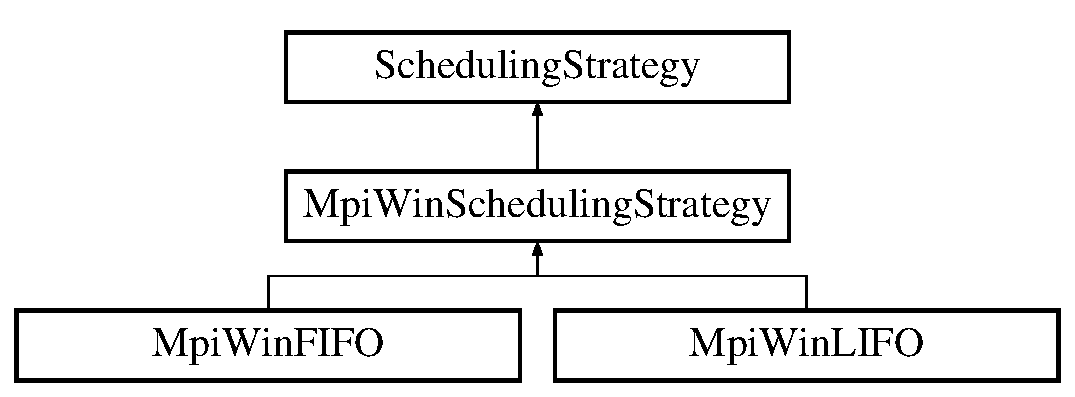
\includegraphics[height=3.000000cm]{class_mpi_win_scheduling_strategy}
\end{center}
\end{figure}
\subsection*{Public Member Functions}
\begin{DoxyCompactItemize}
\item 
virtual \hyperlink{_types_8h_a0c77930ab3818a1680c59353f627fba8}{Task} \hyperlink{class_mpi_win_scheduling_strategy_ac1804574e61c9ed91c7f78bc48b332ea}{steal\+\_\+next\+\_\+task} (int rank, int number\+\_\+of\+\_\+tries)=0
\item 
virtual int \hyperlink{class_mpi_win_scheduling_strategy_a8742d0d3a2204efe5aa47e39f856dee1}{get\+\_\+task\+\_\+count} (int rank)=0
\end{DoxyCompactItemize}
\subsection*{Additional Inherited Members}


\subsection{Detailed Description}
The \hyperlink{class_mpi_win_scheduling_strategy}{Mpi\+Win\+Scheduling\+Strategy} interface is a specialization of the \hyperlink{class_scheduling_strategy}{Scheduling\+Strategy} interface. The \hyperlink{class_mpi_win_scheduling_strategy}{Mpi\+Win\+Scheduling\+Strategy} interface adds function for remote scheduling queue access. Implementations must provide the \hyperlink{class_mpi_win_scheduling_strategy_ac1804574e61c9ed91c7f78bc48b332ea}{steal\+\_\+next\+\_\+task()} and the get\+\_\+task\+\_\+count function on remote scheduling queues by given rank. The tasks must be kept in a M\+P\+I window to support remote memory access.

\begin{DoxyAuthor}{Author}
Fabio Broghammer 
\end{DoxyAuthor}
\begin{DoxyVersion}{Version}
1.\+0 
\end{DoxyVersion}


Definition at line 17 of file Mpi\+Win\+Scheduling\+Strategy.\+h.



\subsection{Member Function Documentation}
\hypertarget{class_mpi_win_scheduling_strategy_a8742d0d3a2204efe5aa47e39f856dee1}{}\index{Mpi\+Win\+Scheduling\+Strategy@{Mpi\+Win\+Scheduling\+Strategy}!get\+\_\+task\+\_\+count@{get\+\_\+task\+\_\+count}}
\index{get\+\_\+task\+\_\+count@{get\+\_\+task\+\_\+count}!Mpi\+Win\+Scheduling\+Strategy@{Mpi\+Win\+Scheduling\+Strategy}}
\subsubsection[{get\+\_\+task\+\_\+count}]{\setlength{\rightskip}{0pt plus 5cm}virtual int Mpi\+Win\+Scheduling\+Strategy\+::get\+\_\+task\+\_\+count (
\begin{DoxyParamCaption}
\item[{int}]{rank}
\end{DoxyParamCaption}
)\hspace{0.3cm}{\ttfamily [pure virtual]}}\label{class_mpi_win_scheduling_strategy_a8742d0d3a2204efe5aa47e39f856dee1}
Returns the task count of the remote queue of the given rank


\begin{DoxyParams}{Parameters}
{\em rank} & the rank of the remote queue\\
\hline
\end{DoxyParams}
\begin{DoxyReturn}{Returns}
the task count of the remote queue 
\end{DoxyReturn}


Implemented in \hyperlink{class_mpi_win_f_i_f_o_a7481a465167e95e3993251106fe40cb3}{Mpi\+Win\+F\+I\+F\+O}, and \hyperlink{class_mpi_win_l_i_f_o_a4825ff8faf740b1f9e984813c20455ec}{Mpi\+Win\+L\+I\+F\+O}.

\hypertarget{class_mpi_win_scheduling_strategy_ac1804574e61c9ed91c7f78bc48b332ea}{}\index{Mpi\+Win\+Scheduling\+Strategy@{Mpi\+Win\+Scheduling\+Strategy}!steal\+\_\+next\+\_\+task@{steal\+\_\+next\+\_\+task}}
\index{steal\+\_\+next\+\_\+task@{steal\+\_\+next\+\_\+task}!Mpi\+Win\+Scheduling\+Strategy@{Mpi\+Win\+Scheduling\+Strategy}}
\subsubsection[{steal\+\_\+next\+\_\+task}]{\setlength{\rightskip}{0pt plus 5cm}virtual {\bf Task} Mpi\+Win\+Scheduling\+Strategy\+::steal\+\_\+next\+\_\+task (
\begin{DoxyParamCaption}
\item[{int}]{rank, }
\item[{int}]{number\+\_\+of\+\_\+tries}
\end{DoxyParamCaption}
)\hspace{0.3cm}{\ttfamily [pure virtual]}}\label{class_mpi_win_scheduling_strategy_ac1804574e61c9ed91c7f78bc48b332ea}
Steals the next task from the given rank if the queue of the given rank is not empty


\begin{DoxyParams}{Parameters}
{\em rank} & the rank of the remote queue\\
\hline
\end{DoxyParams}
\begin{DoxyReturn}{Returns}
the next task from the given rank or N\+U\+L\+L if the queue is empty 
\end{DoxyReturn}


Implemented in \hyperlink{class_mpi_win_f_i_f_o_a8f4af1f3c3f90b939f3638bf321be3bf}{Mpi\+Win\+F\+I\+F\+O}, and \hyperlink{class_mpi_win_l_i_f_o_a0631b1fc2042f19a5b438c8cfa44934a}{Mpi\+Win\+L\+I\+F\+O}.



The documentation for this class was generated from the following file\+:\begin{DoxyCompactItemize}
\item 
src/scheduler/\hyperlink{_mpi_win_scheduling_strategy_8h}{Mpi\+Win\+Scheduling\+Strategy.\+h}\end{DoxyCompactItemize}

\hypertarget{classel_1_1base_1_1_no_copy}{}\section{el\+:\+:base\+:\+:No\+Copy Class Reference}
\label{classel_1_1base_1_1_no_copy}\index{el\+::base\+::\+No\+Copy@{el\+::base\+::\+No\+Copy}}


Internal helper class that prevent copy constructor for class.  




{\ttfamily \#include $<$easylogging++.\+h$>$}

Inheritance diagram for el\+:\+:base\+:\+:No\+Copy\+:\begin{figure}[H]
\begin{center}
\leavevmode
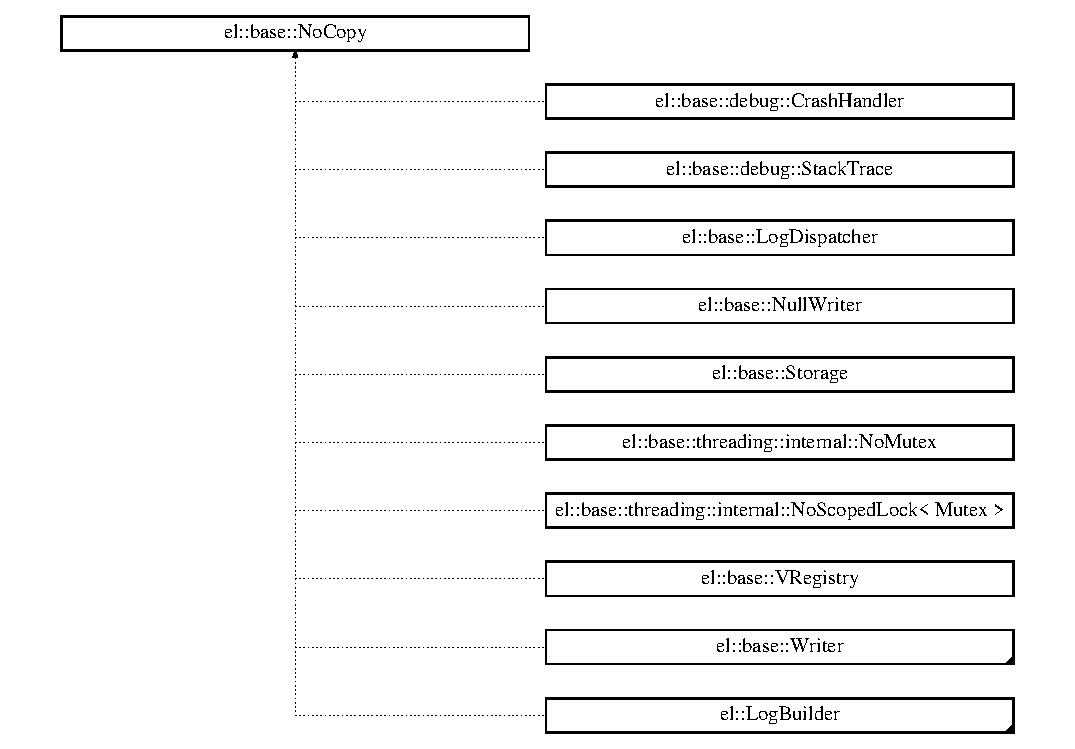
\includegraphics[height=9.625000cm]{classel_1_1base_1_1_no_copy}
\end{center}
\end{figure}
\subsection*{Protected Member Functions}
\begin{DoxyCompactItemize}
\item 
\hyperlink{classel_1_1base_1_1_no_copy_a8a0bc86c5c2b921a3c5fcf6e4d2670d3}{No\+Copy} (void)
\end{DoxyCompactItemize}


\subsection{Detailed Description}
Internal helper class that prevent copy constructor for class. 

When using this class simply inherit it privately 

Definition at line 480 of file easylogging++.\+h.



\subsection{Constructor \& Destructor Documentation}
\hypertarget{classel_1_1base_1_1_no_copy_a8a0bc86c5c2b921a3c5fcf6e4d2670d3}{}\index{el\+::base\+::\+No\+Copy@{el\+::base\+::\+No\+Copy}!No\+Copy@{No\+Copy}}
\index{No\+Copy@{No\+Copy}!el\+::base\+::\+No\+Copy@{el\+::base\+::\+No\+Copy}}
\subsubsection[{No\+Copy}]{\setlength{\rightskip}{0pt plus 5cm}el\+::base\+::\+No\+Copy\+::\+No\+Copy (
\begin{DoxyParamCaption}
\item[{void}]{}
\end{DoxyParamCaption}
)\hspace{0.3cm}{\ttfamily [inline]}, {\ttfamily [protected]}}\label{classel_1_1base_1_1_no_copy_a8a0bc86c5c2b921a3c5fcf6e4d2670d3}


Definition at line 482 of file easylogging++.\+h.



The documentation for this class was generated from the following file\+:\begin{DoxyCompactItemize}
\item 
lib/\hyperlink{easylogging_09_09_8h}{easylogging++.\+h}\end{DoxyCompactItemize}

\hypertarget{classel_1_1base_1_1threading_1_1internal_1_1_no_mutex}{}\section{el\+:\+:base\+:\+:threading\+:\+:internal\+:\+:No\+Mutex Class Reference}
\label{classel_1_1base_1_1threading_1_1internal_1_1_no_mutex}\index{el\+::base\+::threading\+::internal\+::\+No\+Mutex@{el\+::base\+::threading\+::internal\+::\+No\+Mutex}}


Mutex wrapper used when multi-\/threading is disabled.  




{\ttfamily \#include $<$easylogging++.\+h$>$}

Inheritance diagram for el\+:\+:base\+:\+:threading\+:\+:internal\+:\+:No\+Mutex\+:\begin{figure}[H]
\begin{center}
\leavevmode
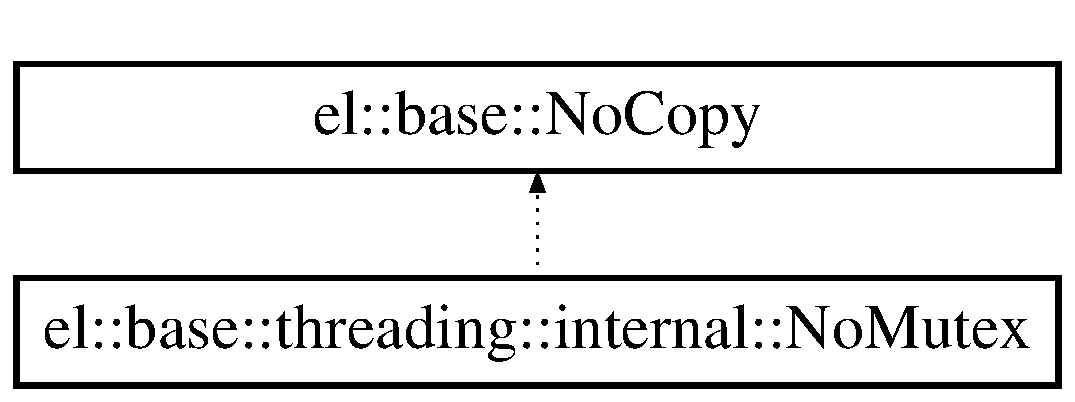
\includegraphics[height=2.000000cm]{classel_1_1base_1_1threading_1_1internal_1_1_no_mutex}
\end{center}
\end{figure}
\subsection*{Public Member Functions}
\begin{DoxyCompactItemize}
\item 
\hyperlink{classel_1_1base_1_1threading_1_1internal_1_1_no_mutex_a23985cbf635efacb39f2a789d539bd29}{No\+Mutex} (void)
\item 
void \hyperlink{classel_1_1base_1_1threading_1_1internal_1_1_no_mutex_a3b38e4e9411c924daa70d358cf561b3c}{lock} (void)
\item 
bool \hyperlink{classel_1_1base_1_1threading_1_1internal_1_1_no_mutex_a4c0c35a99cf41f26a7608fed5609d6ae}{try\+\_\+lock} (void)
\item 
void \hyperlink{classel_1_1base_1_1threading_1_1internal_1_1_no_mutex_a5a248c97fee2ef0087526f2f8d3cd26e}{unlock} (void)
\end{DoxyCompactItemize}


\subsection{Detailed Description}
Mutex wrapper used when multi-\/threading is disabled. 

Definition at line 1041 of file easylogging++.\+h.



\subsection{Constructor \& Destructor Documentation}
\hypertarget{classel_1_1base_1_1threading_1_1internal_1_1_no_mutex_a23985cbf635efacb39f2a789d539bd29}{}\index{el\+::base\+::threading\+::internal\+::\+No\+Mutex@{el\+::base\+::threading\+::internal\+::\+No\+Mutex}!No\+Mutex@{No\+Mutex}}
\index{No\+Mutex@{No\+Mutex}!el\+::base\+::threading\+::internal\+::\+No\+Mutex@{el\+::base\+::threading\+::internal\+::\+No\+Mutex}}
\subsubsection[{No\+Mutex}]{\setlength{\rightskip}{0pt plus 5cm}el\+::base\+::threading\+::internal\+::\+No\+Mutex\+::\+No\+Mutex (
\begin{DoxyParamCaption}
\item[{void}]{}
\end{DoxyParamCaption}
)\hspace{0.3cm}{\ttfamily [inline]}}\label{classel_1_1base_1_1threading_1_1internal_1_1_no_mutex_a23985cbf635efacb39f2a789d539bd29}


Definition at line 1043 of file easylogging++.\+h.



\subsection{Member Function Documentation}
\hypertarget{classel_1_1base_1_1threading_1_1internal_1_1_no_mutex_a3b38e4e9411c924daa70d358cf561b3c}{}\index{el\+::base\+::threading\+::internal\+::\+No\+Mutex@{el\+::base\+::threading\+::internal\+::\+No\+Mutex}!lock@{lock}}
\index{lock@{lock}!el\+::base\+::threading\+::internal\+::\+No\+Mutex@{el\+::base\+::threading\+::internal\+::\+No\+Mutex}}
\subsubsection[{lock}]{\setlength{\rightskip}{0pt plus 5cm}void el\+::base\+::threading\+::internal\+::\+No\+Mutex\+::lock (
\begin{DoxyParamCaption}
\item[{void}]{}
\end{DoxyParamCaption}
)\hspace{0.3cm}{\ttfamily [inline]}}\label{classel_1_1base_1_1threading_1_1internal_1_1_no_mutex_a3b38e4e9411c924daa70d358cf561b3c}


Definition at line 1044 of file easylogging++.\+h.

\hypertarget{classel_1_1base_1_1threading_1_1internal_1_1_no_mutex_a4c0c35a99cf41f26a7608fed5609d6ae}{}\index{el\+::base\+::threading\+::internal\+::\+No\+Mutex@{el\+::base\+::threading\+::internal\+::\+No\+Mutex}!try\+\_\+lock@{try\+\_\+lock}}
\index{try\+\_\+lock@{try\+\_\+lock}!el\+::base\+::threading\+::internal\+::\+No\+Mutex@{el\+::base\+::threading\+::internal\+::\+No\+Mutex}}
\subsubsection[{try\+\_\+lock}]{\setlength{\rightskip}{0pt plus 5cm}bool el\+::base\+::threading\+::internal\+::\+No\+Mutex\+::try\+\_\+lock (
\begin{DoxyParamCaption}
\item[{void}]{}
\end{DoxyParamCaption}
)\hspace{0.3cm}{\ttfamily [inline]}}\label{classel_1_1base_1_1threading_1_1internal_1_1_no_mutex_a4c0c35a99cf41f26a7608fed5609d6ae}


Definition at line 1045 of file easylogging++.\+h.

\hypertarget{classel_1_1base_1_1threading_1_1internal_1_1_no_mutex_a5a248c97fee2ef0087526f2f8d3cd26e}{}\index{el\+::base\+::threading\+::internal\+::\+No\+Mutex@{el\+::base\+::threading\+::internal\+::\+No\+Mutex}!unlock@{unlock}}
\index{unlock@{unlock}!el\+::base\+::threading\+::internal\+::\+No\+Mutex@{el\+::base\+::threading\+::internal\+::\+No\+Mutex}}
\subsubsection[{unlock}]{\setlength{\rightskip}{0pt plus 5cm}void el\+::base\+::threading\+::internal\+::\+No\+Mutex\+::unlock (
\begin{DoxyParamCaption}
\item[{void}]{}
\end{DoxyParamCaption}
)\hspace{0.3cm}{\ttfamily [inline]}}\label{classel_1_1base_1_1threading_1_1internal_1_1_no_mutex_a5a248c97fee2ef0087526f2f8d3cd26e}


Definition at line 1046 of file easylogging++.\+h.



The documentation for this class was generated from the following file\+:\begin{DoxyCompactItemize}
\item 
lib/\hyperlink{easylogging_09_09_8h}{easylogging++.\+h}\end{DoxyCompactItemize}

\hypertarget{classel_1_1base_1_1threading_1_1internal_1_1_no_scoped_lock}{}\section{el\+:\+:base\+:\+:threading\+:\+:internal\+:\+:No\+Scoped\+Lock$<$ Mutex $>$ Class Template Reference}
\label{classel_1_1base_1_1threading_1_1internal_1_1_no_scoped_lock}\index{el\+::base\+::threading\+::internal\+::\+No\+Scoped\+Lock$<$ Mutex $>$@{el\+::base\+::threading\+::internal\+::\+No\+Scoped\+Lock$<$ Mutex $>$}}


Lock guard wrapper used when multi-\/threading is disabled.  




{\ttfamily \#include $<$easylogging++.\+h$>$}

Inheritance diagram for el\+:\+:base\+:\+:threading\+:\+:internal\+:\+:No\+Scoped\+Lock$<$ Mutex $>$\+:\begin{figure}[H]
\begin{center}
\leavevmode
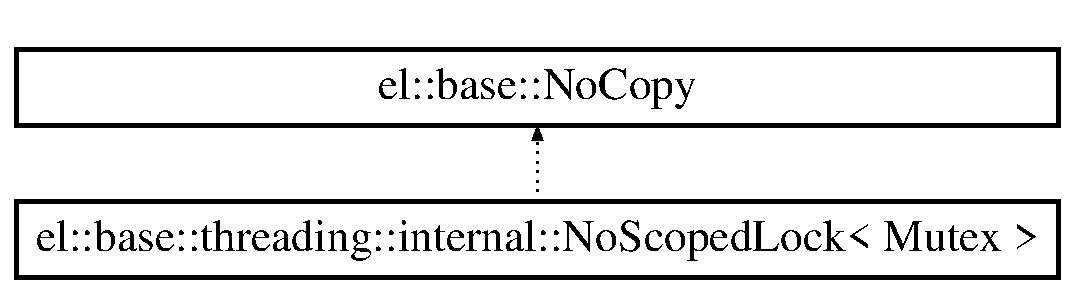
\includegraphics[height=2.000000cm]{classel_1_1base_1_1threading_1_1internal_1_1_no_scoped_lock}
\end{center}
\end{figure}
\subsection*{Public Member Functions}
\begin{DoxyCompactItemize}
\item 
\hyperlink{classel_1_1base_1_1threading_1_1internal_1_1_no_scoped_lock_a020f8cea6e83f40ea29662ef57a58235}{No\+Scoped\+Lock} (\hyperlink{namespaceel_1_1base_1_1threading_ab9400eb234a82878e8458a65f9774320}{Mutex} \&)
\item 
virtual \hyperlink{classel_1_1base_1_1threading_1_1internal_1_1_no_scoped_lock_ae51ca0f4952dd1e99322cda553f472e8}{$\sim$\+No\+Scoped\+Lock} (void)
\end{DoxyCompactItemize}


\subsection{Detailed Description}
\subsubsection*{template$<$typename Mutex$>$class el\+::base\+::threading\+::internal\+::\+No\+Scoped\+Lock$<$ Mutex $>$}

Lock guard wrapper used when multi-\/threading is disabled. 

Definition at line 1050 of file easylogging++.\+h.



\subsection{Constructor \& Destructor Documentation}
\hypertarget{classel_1_1base_1_1threading_1_1internal_1_1_no_scoped_lock_a020f8cea6e83f40ea29662ef57a58235}{}\index{el\+::base\+::threading\+::internal\+::\+No\+Scoped\+Lock@{el\+::base\+::threading\+::internal\+::\+No\+Scoped\+Lock}!No\+Scoped\+Lock@{No\+Scoped\+Lock}}
\index{No\+Scoped\+Lock@{No\+Scoped\+Lock}!el\+::base\+::threading\+::internal\+::\+No\+Scoped\+Lock@{el\+::base\+::threading\+::internal\+::\+No\+Scoped\+Lock}}
\subsubsection[{No\+Scoped\+Lock}]{\setlength{\rightskip}{0pt plus 5cm}template$<$typename Mutex $>$ {\bf el\+::base\+::threading\+::internal\+::\+No\+Scoped\+Lock}$<$ {\bf Mutex} $>$\+::{\bf No\+Scoped\+Lock} (
\begin{DoxyParamCaption}
\item[{{\bf Mutex} \&}]{}
\end{DoxyParamCaption}
)\hspace{0.3cm}{\ttfamily [inline]}, {\ttfamily [explicit]}}\label{classel_1_1base_1_1threading_1_1internal_1_1_no_scoped_lock_a020f8cea6e83f40ea29662ef57a58235}


Definition at line 1052 of file easylogging++.\+h.

\hypertarget{classel_1_1base_1_1threading_1_1internal_1_1_no_scoped_lock_ae51ca0f4952dd1e99322cda553f472e8}{}\index{el\+::base\+::threading\+::internal\+::\+No\+Scoped\+Lock@{el\+::base\+::threading\+::internal\+::\+No\+Scoped\+Lock}!````~No\+Scoped\+Lock@{$\sim$\+No\+Scoped\+Lock}}
\index{````~No\+Scoped\+Lock@{$\sim$\+No\+Scoped\+Lock}!el\+::base\+::threading\+::internal\+::\+No\+Scoped\+Lock@{el\+::base\+::threading\+::internal\+::\+No\+Scoped\+Lock}}
\subsubsection[{$\sim$\+No\+Scoped\+Lock}]{\setlength{\rightskip}{0pt plus 5cm}template$<$typename Mutex $>$ virtual {\bf el\+::base\+::threading\+::internal\+::\+No\+Scoped\+Lock}$<$ {\bf Mutex} $>$\+::$\sim${\bf No\+Scoped\+Lock} (
\begin{DoxyParamCaption}
\item[{void}]{}
\end{DoxyParamCaption}
)\hspace{0.3cm}{\ttfamily [inline]}, {\ttfamily [virtual]}}\label{classel_1_1base_1_1threading_1_1internal_1_1_no_scoped_lock_ae51ca0f4952dd1e99322cda553f472e8}


Definition at line 1054 of file easylogging++.\+h.



The documentation for this class was generated from the following file\+:\begin{DoxyCompactItemize}
\item 
lib/\hyperlink{easylogging_09_09_8h}{easylogging++.\+h}\end{DoxyCompactItemize}

\hypertarget{classel_1_1base_1_1_null_writer}{}\section{el\+:\+:base\+:\+:Null\+Writer Class Reference}
\label{classel_1_1base_1_1_null_writer}\index{el\+::base\+::\+Null\+Writer@{el\+::base\+::\+Null\+Writer}}


Writes nothing -\/ Used when certain log is disabled.  




{\ttfamily \#include $<$easylogging++.\+h$>$}

Inheritance diagram for el\+:\+:base\+:\+:Null\+Writer\+:\begin{figure}[H]
\begin{center}
\leavevmode
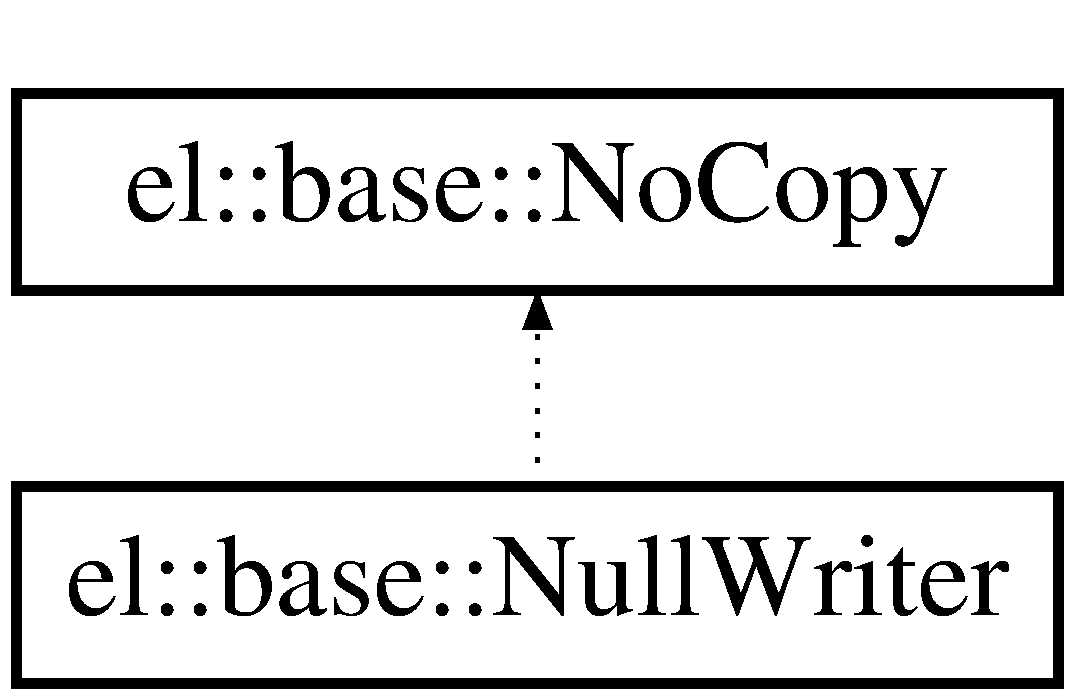
\includegraphics[height=2.000000cm]{classel_1_1base_1_1_null_writer}
\end{center}
\end{figure}
\subsection*{Public Member Functions}
\begin{DoxyCompactItemize}
\item 
\hyperlink{classel_1_1base_1_1_null_writer_a936572812bfcd5a34ed928f11cac9e22}{Null\+Writer} (void)
\item 
\hyperlink{classel_1_1base_1_1_null_writer}{Null\+Writer} \& \hyperlink{classel_1_1base_1_1_null_writer_a39cb7d47986d70c2b4e9d78d1482da7d}{operator$<$$<$} (std\+::ostream \&($\ast$)(std\+::ostream \&))
\item 
{\footnotesize template$<$typename T $>$ }\\\hyperlink{classel_1_1base_1_1_null_writer}{Null\+Writer} \& \hyperlink{classel_1_1base_1_1_null_writer_a57cb0f5d93ebac076b8ef94d6eff65a2}{operator$<$$<$} (const T \&)
\end{DoxyCompactItemize}


\subsection{Detailed Description}
Writes nothing -\/ Used when certain log is disabled. 

Definition at line 4892 of file easylogging++.\+h.



\subsection{Constructor \& Destructor Documentation}
\hypertarget{classel_1_1base_1_1_null_writer_a936572812bfcd5a34ed928f11cac9e22}{}\index{el\+::base\+::\+Null\+Writer@{el\+::base\+::\+Null\+Writer}!Null\+Writer@{Null\+Writer}}
\index{Null\+Writer@{Null\+Writer}!el\+::base\+::\+Null\+Writer@{el\+::base\+::\+Null\+Writer}}
\subsubsection[{Null\+Writer}]{\setlength{\rightskip}{0pt plus 5cm}el\+::base\+::\+Null\+Writer\+::\+Null\+Writer (
\begin{DoxyParamCaption}
\item[{void}]{}
\end{DoxyParamCaption}
)\hspace{0.3cm}{\ttfamily [inline]}}\label{classel_1_1base_1_1_null_writer_a936572812bfcd5a34ed928f11cac9e22}


Definition at line 4894 of file easylogging++.\+h.



\subsection{Member Function Documentation}
\hypertarget{classel_1_1base_1_1_null_writer_a39cb7d47986d70c2b4e9d78d1482da7d}{}\index{el\+::base\+::\+Null\+Writer@{el\+::base\+::\+Null\+Writer}!operator$<$$<$@{operator$<$$<$}}
\index{operator$<$$<$@{operator$<$$<$}!el\+::base\+::\+Null\+Writer@{el\+::base\+::\+Null\+Writer}}
\subsubsection[{operator$<$$<$}]{\setlength{\rightskip}{0pt plus 5cm}{\bf Null\+Writer}\& el\+::base\+::\+Null\+Writer\+::operator$<$$<$ (
\begin{DoxyParamCaption}
\item[{std\+::ostream \&}]{$\ast$)(std\+::ostream \&}
\end{DoxyParamCaption}
)\hspace{0.3cm}{\ttfamily [inline]}}\label{classel_1_1base_1_1_null_writer_a39cb7d47986d70c2b4e9d78d1482da7d}


Definition at line 4897 of file easylogging++.\+h.

\hypertarget{classel_1_1base_1_1_null_writer_a57cb0f5d93ebac076b8ef94d6eff65a2}{}\index{el\+::base\+::\+Null\+Writer@{el\+::base\+::\+Null\+Writer}!operator$<$$<$@{operator$<$$<$}}
\index{operator$<$$<$@{operator$<$$<$}!el\+::base\+::\+Null\+Writer@{el\+::base\+::\+Null\+Writer}}
\subsubsection[{operator$<$$<$}]{\setlength{\rightskip}{0pt plus 5cm}template$<$typename T $>$ {\bf Null\+Writer}\& el\+::base\+::\+Null\+Writer\+::operator$<$$<$ (
\begin{DoxyParamCaption}
\item[{const T \&}]{}
\end{DoxyParamCaption}
)\hspace{0.3cm}{\ttfamily [inline]}}\label{classel_1_1base_1_1_null_writer_a57cb0f5d93ebac076b8ef94d6eff65a2}


Definition at line 4902 of file easylogging++.\+h.



The documentation for this class was generated from the following file\+:\begin{DoxyCompactItemize}
\item 
lib/\hyperlink{easylogging_09_09_8h}{easylogging++.\+h}\end{DoxyCompactItemize}

\hypertarget{classel_1_1base_1_1utils_1_1_o_s}{}\section{el\+:\+:base\+:\+:utils\+:\+:O\+S Class Reference}
\label{classel_1_1base_1_1utils_1_1_o_s}\index{el\+::base\+::utils\+::\+O\+S@{el\+::base\+::utils\+::\+O\+S}}


Operating System helper static class used internally. You should not use it.  




{\ttfamily \#include $<$easylogging++.\+h$>$}

Inheritance diagram for el\+:\+:base\+:\+:utils\+:\+:O\+S\+:\begin{figure}[H]
\begin{center}
\leavevmode
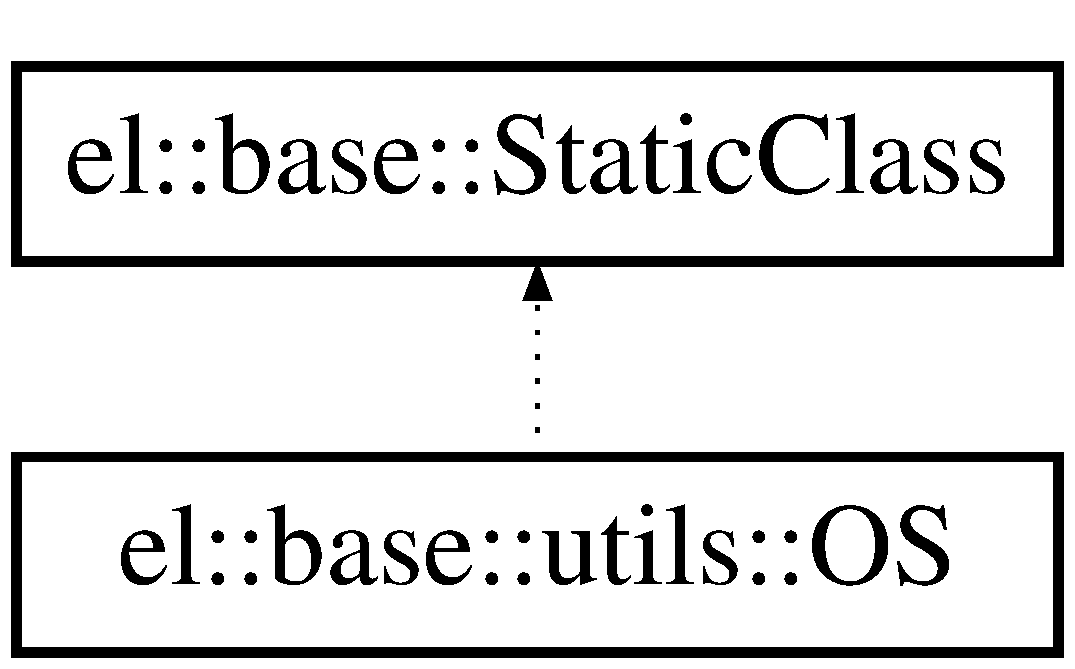
\includegraphics[height=2.000000cm]{classel_1_1base_1_1utils_1_1_o_s}
\end{center}
\end{figure}
\subsection*{Static Public Member Functions}
\begin{DoxyCompactItemize}
\item 
static const std\+::string \hyperlink{classel_1_1base_1_1utils_1_1_o_s_a91304c76c872459eaa9fdb3466367cd3}{get\+Bash\+Output} (const char $\ast$command)
\begin{DoxyCompactList}\small\item\em Runs command on terminal and returns the output. \end{DoxyCompactList}\item 
static std\+::string \hyperlink{classel_1_1base_1_1utils_1_1_o_s_a91540f3d8c87bd121e55fc39270eac3c}{get\+Environment\+Variable} (const char $\ast$variable\+Name, const char $\ast$default\+Val, const char $\ast$alternative\+Bash\+Command=nullptr)
\begin{DoxyCompactList}\small\item\em Gets environment variable. This is cross-\/platform and C\+R\+T safe (for V\+C++) \end{DoxyCompactList}\item 
static std\+::string \hyperlink{classel_1_1base_1_1utils_1_1_o_s_ac7839ecd50e379dbdfcfce130906386e}{current\+User} (void)
\begin{DoxyCompactList}\small\item\em Gets current username. \end{DoxyCompactList}\item 
static std\+::string \hyperlink{classel_1_1base_1_1utils_1_1_o_s_aae4fdf83828228fc440f8a875c5942b0}{current\+Host} (void)
\begin{DoxyCompactList}\small\item\em Gets current host name or computer name. \end{DoxyCompactList}\item 
static bool \hyperlink{classel_1_1base_1_1utils_1_1_o_s_a2c941329a14ce0ea920f57779857864c}{term\+Supports\+Color} (void)
\begin{DoxyCompactList}\small\item\em Whether or not terminal supports colors. \end{DoxyCompactList}\end{DoxyCompactItemize}


\subsection{Detailed Description}
Operating System helper static class used internally. You should not use it. 

Definition at line 1418 of file easylogging++.\+h.



\subsection{Member Function Documentation}
\hypertarget{classel_1_1base_1_1utils_1_1_o_s_aae4fdf83828228fc440f8a875c5942b0}{}\index{el\+::base\+::utils\+::\+O\+S@{el\+::base\+::utils\+::\+O\+S}!current\+Host@{current\+Host}}
\index{current\+Host@{current\+Host}!el\+::base\+::utils\+::\+O\+S@{el\+::base\+::utils\+::\+O\+S}}
\subsubsection[{current\+Host}]{\setlength{\rightskip}{0pt plus 5cm}static std\+::string el\+::base\+::utils\+::\+O\+S\+::current\+Host (
\begin{DoxyParamCaption}
\item[{void}]{}
\end{DoxyParamCaption}
)\hspace{0.3cm}{\ttfamily [inline]}, {\ttfamily [static]}}\label{classel_1_1base_1_1utils_1_1_o_s_aae4fdf83828228fc440f8a875c5942b0}


Gets current host name or computer name. 

For android systems this is device name with its manufacturer and model seperated by hyphen 

Definition at line 1529 of file easylogging++.\+h.

\hypertarget{classel_1_1base_1_1utils_1_1_o_s_ac7839ecd50e379dbdfcfce130906386e}{}\index{el\+::base\+::utils\+::\+O\+S@{el\+::base\+::utils\+::\+O\+S}!current\+User@{current\+User}}
\index{current\+User@{current\+User}!el\+::base\+::utils\+::\+O\+S@{el\+::base\+::utils\+::\+O\+S}}
\subsubsection[{current\+User}]{\setlength{\rightskip}{0pt plus 5cm}static std\+::string el\+::base\+::utils\+::\+O\+S\+::current\+User (
\begin{DoxyParamCaption}
\item[{void}]{}
\end{DoxyParamCaption}
)\hspace{0.3cm}{\ttfamily [inline]}, {\ttfamily [static]}}\label{classel_1_1base_1_1utils_1_1_o_s_ac7839ecd50e379dbdfcfce130906386e}


Gets current username. 



Definition at line 1513 of file easylogging++.\+h.

\hypertarget{classel_1_1base_1_1utils_1_1_o_s_a91304c76c872459eaa9fdb3466367cd3}{}\index{el\+::base\+::utils\+::\+O\+S@{el\+::base\+::utils\+::\+O\+S}!get\+Bash\+Output@{get\+Bash\+Output}}
\index{get\+Bash\+Output@{get\+Bash\+Output}!el\+::base\+::utils\+::\+O\+S@{el\+::base\+::utils\+::\+O\+S}}
\subsubsection[{get\+Bash\+Output}]{\setlength{\rightskip}{0pt plus 5cm}static const std\+::string el\+::base\+::utils\+::\+O\+S\+::get\+Bash\+Output (
\begin{DoxyParamCaption}
\item[{const char $\ast$}]{command}
\end{DoxyParamCaption}
)\hspace{0.3cm}{\ttfamily [inline]}, {\ttfamily [static]}}\label{classel_1_1base_1_1utils_1_1_o_s_a91304c76c872459eaa9fdb3466367cd3}


Runs command on terminal and returns the output. 

This is applicable only on unix based systems, for all other \hyperlink{classel_1_1base_1_1utils_1_1_o_s}{O\+S}, an empty string is returned. 
\begin{DoxyParams}{Parameters}
{\em command} & Bash command \\
\hline
\end{DoxyParams}
\begin{DoxyReturn}{Returns}
Result of bash output or empty string if no result found. 
\end{DoxyReturn}


Definition at line 1460 of file easylogging++.\+h.

\hypertarget{classel_1_1base_1_1utils_1_1_o_s_a91540f3d8c87bd121e55fc39270eac3c}{}\index{el\+::base\+::utils\+::\+O\+S@{el\+::base\+::utils\+::\+O\+S}!get\+Environment\+Variable@{get\+Environment\+Variable}}
\index{get\+Environment\+Variable@{get\+Environment\+Variable}!el\+::base\+::utils\+::\+O\+S@{el\+::base\+::utils\+::\+O\+S}}
\subsubsection[{get\+Environment\+Variable}]{\setlength{\rightskip}{0pt plus 5cm}static std\+::string el\+::base\+::utils\+::\+O\+S\+::get\+Environment\+Variable (
\begin{DoxyParamCaption}
\item[{const char $\ast$}]{variable\+Name, }
\item[{const char $\ast$}]{default\+Val, }
\item[{const char $\ast$}]{alternative\+Bash\+Command = {\ttfamily nullptr}}
\end{DoxyParamCaption}
)\hspace{0.3cm}{\ttfamily [inline]}, {\ttfamily [static]}}\label{classel_1_1base_1_1utils_1_1_o_s_a91540f3d8c87bd121e55fc39270eac3c}


Gets environment variable. This is cross-\/platform and C\+R\+T safe (for V\+C++) 


\begin{DoxyParams}{Parameters}
{\em variable\+Name} & Environment variable name \\
\hline
{\em default\+Val} & If no environment variable or value found the value to return by default \\
\hline
{\em alternative\+Bash\+Command} & If environment variable not found what would be alternative bash command in order to look for value user is looking for. E.\+g, for \textquotesingle{}user\textquotesingle{} alternative command will \textquotesingle{}whoami\textquotesingle{} \\
\hline
\end{DoxyParams}


Definition at line 1490 of file easylogging++.\+h.

\hypertarget{classel_1_1base_1_1utils_1_1_o_s_a2c941329a14ce0ea920f57779857864c}{}\index{el\+::base\+::utils\+::\+O\+S@{el\+::base\+::utils\+::\+O\+S}!term\+Supports\+Color@{term\+Supports\+Color}}
\index{term\+Supports\+Color@{term\+Supports\+Color}!el\+::base\+::utils\+::\+O\+S@{el\+::base\+::utils\+::\+O\+S}}
\subsubsection[{term\+Supports\+Color}]{\setlength{\rightskip}{0pt plus 5cm}static bool el\+::base\+::utils\+::\+O\+S\+::term\+Supports\+Color (
\begin{DoxyParamCaption}
\item[{void}]{}
\end{DoxyParamCaption}
)\hspace{0.3cm}{\ttfamily [inline]}, {\ttfamily [static]}}\label{classel_1_1base_1_1utils_1_1_o_s_a2c941329a14ce0ea920f57779857864c}


Whether or not terminal supports colors. 



Definition at line 1542 of file easylogging++.\+h.



The documentation for this class was generated from the following file\+:\begin{DoxyCompactItemize}
\item 
lib/\hyperlink{easylogging_09_09_8h}{easylogging++.\+h}\end{DoxyCompactItemize}

\hypertarget{classel_1_1_configurations_1_1_parser}{}\section{el\+:\+:Configurations\+:\+:Parser Class Reference}
\label{classel_1_1_configurations_1_1_parser}\index{el\+::\+Configurations\+::\+Parser@{el\+::\+Configurations\+::\+Parser}}


\hyperlink{classel_1_1_configurations_1_1_parser}{Parser} used internally to parse configurations from file or text.  




{\ttfamily \#include $<$easylogging++.\+h$>$}

Inheritance diagram for el\+:\+:Configurations\+:\+:Parser\+:\begin{figure}[H]
\begin{center}
\leavevmode
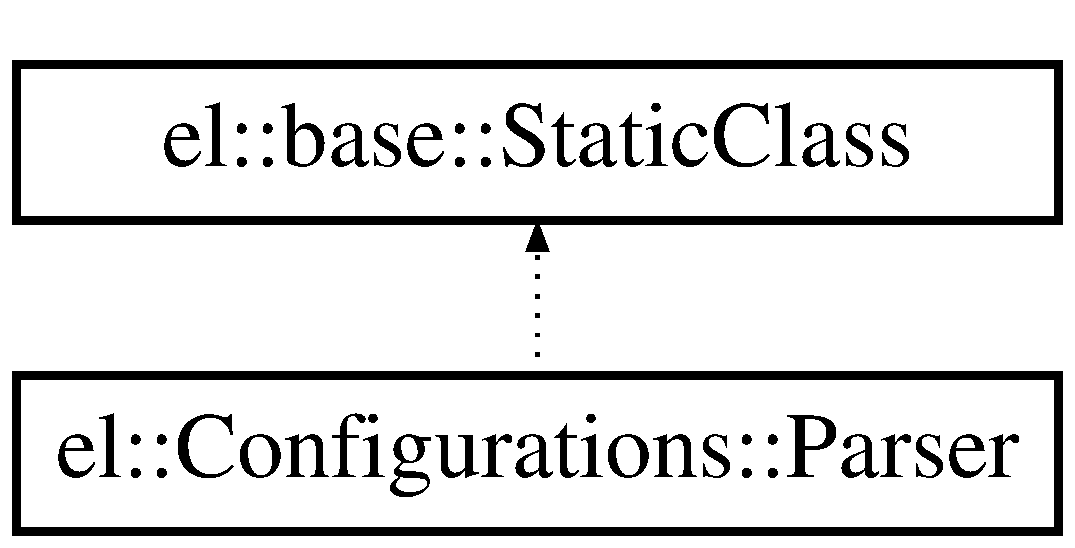
\includegraphics[height=2.000000cm]{classel_1_1_configurations_1_1_parser}
\end{center}
\end{figure}
\subsection*{Static Public Member Functions}
\begin{DoxyCompactItemize}
\item 
static bool \hyperlink{classel_1_1_configurations_1_1_parser_a45def5007bf368c4d2a505af58cd94c2}{parse\+From\+File} (const std\+::string \&\hyperlink{classel_1_1_configurations_a18df64bb5cd97bee672160290133141c}{configuration\+File}, \hyperlink{classel_1_1_configurations}{Configurations} $\ast$sender, \hyperlink{classel_1_1_configurations}{Configurations} $\ast$base=nullptr)
\begin{DoxyCompactList}\small\item\em Parses configuration from file. \end{DoxyCompactList}\item 
static bool \hyperlink{classel_1_1_configurations_1_1_parser_a39ec1b06f673e8155a83d66e08229129}{parse\+From\+Text} (const std\+::string \&configurations\+String, \hyperlink{classel_1_1_configurations}{Configurations} $\ast$sender, \hyperlink{classel_1_1_configurations}{Configurations} $\ast$base=nullptr)
\begin{DoxyCompactList}\small\item\em Parse configurations from configuration string. \end{DoxyCompactList}\end{DoxyCompactItemize}
\subsection*{Friends}
\begin{DoxyCompactItemize}
\item 
class \hyperlink{classel_1_1_configurations_1_1_parser_a6efe246b312d02731fb0e1d120c0331d}{el\+::\+Loggers}
\end{DoxyCompactItemize}


\subsection{Detailed Description}
\hyperlink{classel_1_1_configurations_1_1_parser}{Parser} used internally to parse configurations from file or text. 

This class makes use of \hyperlink{classel_1_1base_1_1utils_1_1_str}{base\+::utils\+::\+Str}. You should not need this unless you are working on some tool for Easylogging++ 

Definition at line 2652 of file easylogging++.\+h.



\subsection{Member Function Documentation}
\hypertarget{classel_1_1_configurations_1_1_parser_a45def5007bf368c4d2a505af58cd94c2}{}\index{el\+::\+Configurations\+::\+Parser@{el\+::\+Configurations\+::\+Parser}!parse\+From\+File@{parse\+From\+File}}
\index{parse\+From\+File@{parse\+From\+File}!el\+::\+Configurations\+::\+Parser@{el\+::\+Configurations\+::\+Parser}}
\subsubsection[{parse\+From\+File}]{\setlength{\rightskip}{0pt plus 5cm}static bool el\+::\+Configurations\+::\+Parser\+::parse\+From\+File (
\begin{DoxyParamCaption}
\item[{const std\+::string \&}]{configuration\+File, }
\item[{{\bf Configurations} $\ast$}]{sender, }
\item[{{\bf Configurations} $\ast$}]{base = {\ttfamily nullptr}}
\end{DoxyParamCaption}
)\hspace{0.3cm}{\ttfamily [inline]}, {\ttfamily [static]}}\label{classel_1_1_configurations_1_1_parser_a45def5007bf368c4d2a505af58cd94c2}


Parses configuration from file. 


\begin{DoxyParams}{Parameters}
{\em configuration\+File} & Full path to configuration file \\
\hline
{\em sender} & Sender configurations pointer. Usually \textquotesingle{}this\textquotesingle{} is used from calling class \\
\hline
{\em base} & \hyperlink{classel_1_1_configurations}{Configurations} to base new configuration repository off. This value is used when you want to use existing \hyperlink{classel_1_1_configurations}{Configurations} to base all the values and then set rest of configuration via configuration file. \\
\hline
\end{DoxyParams}
\begin{DoxyReturn}{Returns}
True if successfully parsed, false otherwise. You may define \textquotesingle{}\+\_\+\+S\+T\+O\+P\+\_\+\+O\+N\+\_\+\+F\+I\+R\+S\+T\+E\+L\+P\+P\+\_\+\+A\+S\+S\+E\+R\+T\+I\+O\+N\textquotesingle{} to make sure you do not proceed without successful parse. 
\end{DoxyReturn}


Definition at line 2661 of file easylogging++.\+h.

\hypertarget{classel_1_1_configurations_1_1_parser_a39ec1b06f673e8155a83d66e08229129}{}\index{el\+::\+Configurations\+::\+Parser@{el\+::\+Configurations\+::\+Parser}!parse\+From\+Text@{parse\+From\+Text}}
\index{parse\+From\+Text@{parse\+From\+Text}!el\+::\+Configurations\+::\+Parser@{el\+::\+Configurations\+::\+Parser}}
\subsubsection[{parse\+From\+Text}]{\setlength{\rightskip}{0pt plus 5cm}static bool el\+::\+Configurations\+::\+Parser\+::parse\+From\+Text (
\begin{DoxyParamCaption}
\item[{const std\+::string \&}]{configurations\+String, }
\item[{{\bf Configurations} $\ast$}]{sender, }
\item[{{\bf Configurations} $\ast$}]{base = {\ttfamily nullptr}}
\end{DoxyParamCaption}
)\hspace{0.3cm}{\ttfamily [inline]}, {\ttfamily [static]}}\label{classel_1_1_configurations_1_1_parser_a39ec1b06f673e8155a83d66e08229129}


Parse configurations from configuration string. 

This configuration string has same syntax as configuration file contents. Make sure all the necessary new line characters are provided. You may define \textquotesingle{}\+\_\+\+S\+T\+O\+P\+\_\+\+O\+N\+\_\+\+F\+I\+R\+S\+T\+E\+L\+P\+P\+\_\+\+A\+S\+S\+E\+R\+T\+I\+O\+N\textquotesingle{} to make sure you do not proceed without successful parse (This is recommended) 
\begin{DoxyParams}{Parameters}
{\em configurations\+String} & \\
\hline
{\em sender} & Sender configurations pointer. Usually \textquotesingle{}this\textquotesingle{} is used from calling class \\
\hline
{\em base} & \hyperlink{classel_1_1_configurations}{Configurations} to base new configuration repository off. This value is used when you want to use existing \hyperlink{classel_1_1_configurations}{Configurations} to base all the values and then set rest of configuration via configuration text. \\
\hline
\end{DoxyParams}
\begin{DoxyReturn}{Returns}
True if successfully parsed, false otherwise. 
\end{DoxyReturn}


Definition at line 2688 of file easylogging++.\+h.



\subsection{Friends And Related Function Documentation}
\hypertarget{classel_1_1_configurations_1_1_parser_a6efe246b312d02731fb0e1d120c0331d}{}\index{el\+::\+Configurations\+::\+Parser@{el\+::\+Configurations\+::\+Parser}!el\+::\+Loggers@{el\+::\+Loggers}}
\index{el\+::\+Loggers@{el\+::\+Loggers}!el\+::\+Configurations\+::\+Parser@{el\+::\+Configurations\+::\+Parser}}
\subsubsection[{el\+::\+Loggers}]{\setlength{\rightskip}{0pt plus 5cm}friend class {\bf el\+::\+Loggers}\hspace{0.3cm}{\ttfamily [friend]}}\label{classel_1_1_configurations_1_1_parser_a6efe246b312d02731fb0e1d120c0331d}


Definition at line 2704 of file easylogging++.\+h.



The documentation for this class was generated from the following file\+:\begin{DoxyCompactItemize}
\item 
lib/\hyperlink{easylogging_09_09_8h}{easylogging++.\+h}\end{DoxyCompactItemize}

\hypertarget{classel_1_1base_1_1_performance_tracker}{}\section{el\+:\+:base\+:\+:Performance\+Tracker Class Reference}
\label{classel_1_1base_1_1_performance_tracker}\index{el\+::base\+::\+Performance\+Tracker@{el\+::base\+::\+Performance\+Tracker}}


Represents performance\+Tracker block of code that conditionally adds performance status to log either when goes outside the scope of when \hyperlink{classel_1_1base_1_1_performance_tracker_aec9a6e149674c5782cc855e49aeb0aaf}{checkpoint()} is called.  




{\ttfamily \#include $<$easylogging++.\+h$>$}

Inheritance diagram for el\+:\+:base\+:\+:Performance\+Tracker\+:\begin{figure}[H]
\begin{center}
\leavevmode
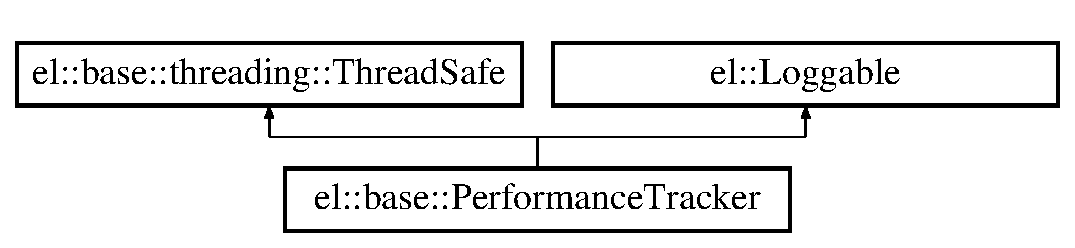
\includegraphics[height=2.000000cm]{classel_1_1base_1_1_performance_tracker}
\end{center}
\end{figure}
\subsection*{Public Member Functions}
\begin{DoxyCompactItemize}
\item 
\hyperlink{classel_1_1base_1_1_performance_tracker_a46ac6a851c6d1cde6742a7ebfeedd1b6}{Performance\+Tracker} (const std\+::string \&block\+Name, \hyperlink{namespaceel_1_1base_a1b886858c6409097395b24b1bdf03c39}{base\+::\+Timestamp\+Unit} timestamp\+Unit=\hyperlink{namespaceel_1_1base_a1b886858c6409097395b24b1bdf03c39a988bbeeb80e7e0a6b4651aab5a76b413}{base\+::\+Timestamp\+Unit\+::\+Millisecond}, const std\+::string \&logger\+Id=std\+::string(\hyperlink{easylogging_09_09_8h_a2ed89aa4136d3c3217697afe1e28fa87}{E\+L\+P\+P\+\_\+\+C\+U\+R\+R\+\_\+\+F\+I\+L\+E\+\_\+\+P\+E\+R\+F\+O\+R\+M\+A\+N\+C\+E\+\_\+\+L\+O\+G\+G\+E\+R}), bool scoped\+Log=true, \hyperlink{namespaceel_ab0ac6091262344c52dd2d3ad099e8e36}{Level} \hyperlink{classel_1_1base_1_1_performance_tracker_a3e0ebd666cc7416dc9b818418266161b}{level}=base\+::consts\+::k\+Performance\+Tracker\+Default\+Level)
\item 
\hyperlink{classel_1_1base_1_1_performance_tracker_a49e655c1f414f904b2d6a9abb0d344f4}{Performance\+Tracker} (const \hyperlink{classel_1_1base_1_1_performance_tracker}{Performance\+Tracker} \&t)
\begin{DoxyCompactList}\small\item\em Copy constructor. \end{DoxyCompactList}\item 
virtual \hyperlink{classel_1_1base_1_1_performance_tracker_a19be0aa65c8623273459185277b52b0c}{$\sim$\+Performance\+Tracker} (void)
\item 
void \hyperlink{classel_1_1base_1_1_performance_tracker_aec9a6e149674c5782cc855e49aeb0aaf}{checkpoint} (const std\+::string \&id=std\+::string(), const char $\ast$file=\+\_\+\+\_\+\+F\+I\+L\+E\+\_\+\+\_\+, unsigned long int line=\+\_\+\+\_\+\+L\+I\+N\+E\+\_\+\+\_\+, const char $\ast$func=\char`\"{}\char`\"{})
\begin{DoxyCompactList}\small\item\em A checkpoint for current performance\+Tracker block. \end{DoxyCompactList}\item 
\hyperlink{namespaceel_ab0ac6091262344c52dd2d3ad099e8e36}{Level} \hyperlink{classel_1_1base_1_1_performance_tracker_a3e0ebd666cc7416dc9b818418266161b}{level} (void) const 
\end{DoxyCompactItemize}
\subsection*{Friends}
\begin{DoxyCompactItemize}
\item 
class \hyperlink{classel_1_1base_1_1_performance_tracker_a7a4da7334b79856c37538484584207a6}{el\+::\+Performance\+Tracking\+Data}
\item 
class \hyperlink{classel_1_1base_1_1_performance_tracker_ad346c4097e3db22a7434e7da5aa9c5e3}{base\+::\+Default\+Performance\+Tracking\+Callback}
\end{DoxyCompactItemize}
\subsection*{Additional Inherited Members}


\subsection{Detailed Description}
Represents performance\+Tracker block of code that conditionally adds performance status to log either when goes outside the scope of when \hyperlink{classel_1_1base_1_1_performance_tracker_aec9a6e149674c5782cc855e49aeb0aaf}{checkpoint()} is called. 

Definition at line 5279 of file easylogging++.\+h.



\subsection{Constructor \& Destructor Documentation}
\hypertarget{classel_1_1base_1_1_performance_tracker_a46ac6a851c6d1cde6742a7ebfeedd1b6}{}\index{el\+::base\+::\+Performance\+Tracker@{el\+::base\+::\+Performance\+Tracker}!Performance\+Tracker@{Performance\+Tracker}}
\index{Performance\+Tracker@{Performance\+Tracker}!el\+::base\+::\+Performance\+Tracker@{el\+::base\+::\+Performance\+Tracker}}
\subsubsection[{Performance\+Tracker}]{\setlength{\rightskip}{0pt plus 5cm}el\+::base\+::\+Performance\+Tracker\+::\+Performance\+Tracker (
\begin{DoxyParamCaption}
\item[{const std\+::string \&}]{block\+Name, }
\item[{{\bf base\+::\+Timestamp\+Unit}}]{timestamp\+Unit = {\ttfamily {\bf base\+::\+Timestamp\+Unit\+::\+Millisecond}}, }
\item[{const std\+::string \&}]{logger\+Id = {\ttfamily std\+:\+:string({\bf E\+L\+P\+P\+\_\+\+C\+U\+R\+R\+\_\+\+F\+I\+L\+E\+\_\+\+P\+E\+R\+F\+O\+R\+M\+A\+N\+C\+E\+\_\+\+L\+O\+G\+G\+E\+R})}, }
\item[{bool}]{scoped\+Log = {\ttfamily true}, }
\item[{{\bf Level}}]{level = {\ttfamily base\+:\+:consts\+:\+:kPerformanceTrackerDefaultLevel}}
\end{DoxyParamCaption}
)\hspace{0.3cm}{\ttfamily [inline]}}\label{classel_1_1base_1_1_performance_tracker_a46ac6a851c6d1cde6742a7ebfeedd1b6}


Definition at line 5281 of file easylogging++.\+h.

\hypertarget{classel_1_1base_1_1_performance_tracker_a49e655c1f414f904b2d6a9abb0d344f4}{}\index{el\+::base\+::\+Performance\+Tracker@{el\+::base\+::\+Performance\+Tracker}!Performance\+Tracker@{Performance\+Tracker}}
\index{Performance\+Tracker@{Performance\+Tracker}!el\+::base\+::\+Performance\+Tracker@{el\+::base\+::\+Performance\+Tracker}}
\subsubsection[{Performance\+Tracker}]{\setlength{\rightskip}{0pt plus 5cm}el\+::base\+::\+Performance\+Tracker\+::\+Performance\+Tracker (
\begin{DoxyParamCaption}
\item[{const {\bf Performance\+Tracker} \&}]{t}
\end{DoxyParamCaption}
)\hspace{0.3cm}{\ttfamily [inline]}}\label{classel_1_1base_1_1_performance_tracker_a49e655c1f414f904b2d6a9abb0d344f4}


Copy constructor. 



Definition at line 5298 of file easylogging++.\+h.

\hypertarget{classel_1_1base_1_1_performance_tracker_a19be0aa65c8623273459185277b52b0c}{}\index{el\+::base\+::\+Performance\+Tracker@{el\+::base\+::\+Performance\+Tracker}!````~Performance\+Tracker@{$\sim$\+Performance\+Tracker}}
\index{````~Performance\+Tracker@{$\sim$\+Performance\+Tracker}!el\+::base\+::\+Performance\+Tracker@{el\+::base\+::\+Performance\+Tracker}}
\subsubsection[{$\sim$\+Performance\+Tracker}]{\setlength{\rightskip}{0pt plus 5cm}virtual el\+::base\+::\+Performance\+Tracker\+::$\sim$\+Performance\+Tracker (
\begin{DoxyParamCaption}
\item[{void}]{}
\end{DoxyParamCaption}
)\hspace{0.3cm}{\ttfamily [inline]}, {\ttfamily [virtual]}}\label{classel_1_1base_1_1_performance_tracker_a19be0aa65c8623273459185277b52b0c}


Definition at line 5303 of file easylogging++.\+h.



\subsection{Member Function Documentation}
\hypertarget{classel_1_1base_1_1_performance_tracker_aec9a6e149674c5782cc855e49aeb0aaf}{}\index{el\+::base\+::\+Performance\+Tracker@{el\+::base\+::\+Performance\+Tracker}!checkpoint@{checkpoint}}
\index{checkpoint@{checkpoint}!el\+::base\+::\+Performance\+Tracker@{el\+::base\+::\+Performance\+Tracker}}
\subsubsection[{checkpoint}]{\setlength{\rightskip}{0pt plus 5cm}void el\+::base\+::\+Performance\+Tracker\+::checkpoint (
\begin{DoxyParamCaption}
\item[{const std\+::string \&}]{id = {\ttfamily std\+:\+:string()}, }
\item[{const char $\ast$}]{file = {\ttfamily \+\_\+\+\_\+FILE\+\_\+\+\_\+}, }
\item[{unsigned long int}]{line = {\ttfamily \+\_\+\+\_\+LINE\+\_\+\+\_\+}, }
\item[{const char $\ast$}]{func = {\ttfamily \char`\"{}\char`\"{}}}
\end{DoxyParamCaption}
)\hspace{0.3cm}{\ttfamily [inline]}}\label{classel_1_1base_1_1_performance_tracker_aec9a6e149674c5782cc855e49aeb0aaf}


A checkpoint for current performance\+Tracker block. 



Definition at line 5328 of file easylogging++.\+h.

\hypertarget{classel_1_1base_1_1_performance_tracker_a3e0ebd666cc7416dc9b818418266161b}{}\index{el\+::base\+::\+Performance\+Tracker@{el\+::base\+::\+Performance\+Tracker}!level@{level}}
\index{level@{level}!el\+::base\+::\+Performance\+Tracker@{el\+::base\+::\+Performance\+Tracker}}
\subsubsection[{level}]{\setlength{\rightskip}{0pt plus 5cm}{\bf Level} el\+::base\+::\+Performance\+Tracker\+::level (
\begin{DoxyParamCaption}
\item[{void}]{}
\end{DoxyParamCaption}
) const\hspace{0.3cm}{\ttfamily [inline]}}\label{classel_1_1base_1_1_performance_tracker_a3e0ebd666cc7416dc9b818418266161b}


Definition at line 5361 of file easylogging++.\+h.



\subsection{Friends And Related Function Documentation}
\hypertarget{classel_1_1base_1_1_performance_tracker_ad346c4097e3db22a7434e7da5aa9c5e3}{}\index{el\+::base\+::\+Performance\+Tracker@{el\+::base\+::\+Performance\+Tracker}!base\+::\+Default\+Performance\+Tracking\+Callback@{base\+::\+Default\+Performance\+Tracking\+Callback}}
\index{base\+::\+Default\+Performance\+Tracking\+Callback@{base\+::\+Default\+Performance\+Tracking\+Callback}!el\+::base\+::\+Performance\+Tracker@{el\+::base\+::\+Performance\+Tracker}}
\subsubsection[{base\+::\+Default\+Performance\+Tracking\+Callback}]{\setlength{\rightskip}{0pt plus 5cm}friend class {\bf base\+::\+Default\+Performance\+Tracking\+Callback}\hspace{0.3cm}{\ttfamily [friend]}}\label{classel_1_1base_1_1_performance_tracker_ad346c4097e3db22a7434e7da5aa9c5e3}


Definition at line 5376 of file easylogging++.\+h.

\hypertarget{classel_1_1base_1_1_performance_tracker_a7a4da7334b79856c37538484584207a6}{}\index{el\+::base\+::\+Performance\+Tracker@{el\+::base\+::\+Performance\+Tracker}!el\+::\+Performance\+Tracking\+Data@{el\+::\+Performance\+Tracking\+Data}}
\index{el\+::\+Performance\+Tracking\+Data@{el\+::\+Performance\+Tracking\+Data}!el\+::base\+::\+Performance\+Tracker@{el\+::base\+::\+Performance\+Tracker}}
\subsubsection[{el\+::\+Performance\+Tracking\+Data}]{\setlength{\rightskip}{0pt plus 5cm}friend class {\bf el\+::\+Performance\+Tracking\+Data}\hspace{0.3cm}{\ttfamily [friend]}}\label{classel_1_1base_1_1_performance_tracker_a7a4da7334b79856c37538484584207a6}


Definition at line 5375 of file easylogging++.\+h.



The documentation for this class was generated from the following file\+:\begin{DoxyCompactItemize}
\item 
lib/\hyperlink{easylogging_09_09_8h}{easylogging++.\+h}\end{DoxyCompactItemize}

\hypertarget{classel_1_1_performance_tracking_callback}{}\section{el\+:\+:Performance\+Tracking\+Callback Class Reference}
\label{classel_1_1_performance_tracking_callback}\index{el\+::\+Performance\+Tracking\+Callback@{el\+::\+Performance\+Tracking\+Callback}}


{\ttfamily \#include $<$easylogging++.\+h$>$}

Inheritance diagram for el\+:\+:Performance\+Tracking\+Callback\+:\begin{figure}[H]
\begin{center}
\leavevmode
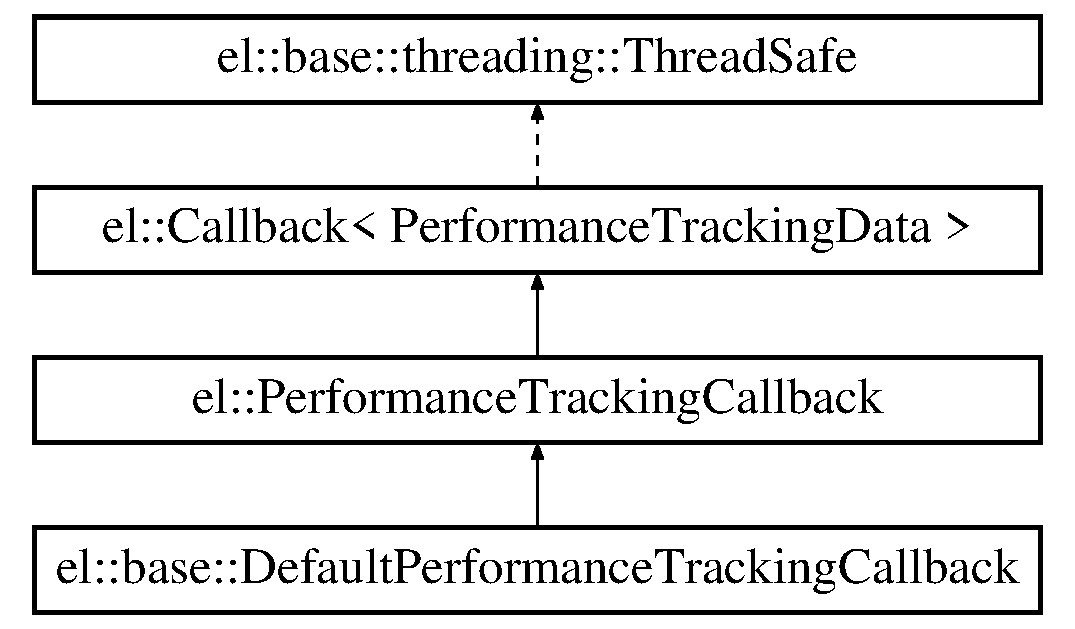
\includegraphics[height=4.000000cm]{classel_1_1_performance_tracking_callback}
\end{center}
\end{figure}
\subsection*{Friends}
\begin{DoxyCompactItemize}
\item 
class \hyperlink{classel_1_1_performance_tracking_callback_a05f271f9cc2531409fe682c6ce0d9feb}{base\+::\+Performance\+Tracker}
\end{DoxyCompactItemize}
\subsection*{Additional Inherited Members}


\subsection{Detailed Description}


Definition at line 3351 of file easylogging++.\+h.



\subsection{Friends And Related Function Documentation}
\hypertarget{classel_1_1_performance_tracking_callback_a05f271f9cc2531409fe682c6ce0d9feb}{}\index{el\+::\+Performance\+Tracking\+Callback@{el\+::\+Performance\+Tracking\+Callback}!base\+::\+Performance\+Tracker@{base\+::\+Performance\+Tracker}}
\index{base\+::\+Performance\+Tracker@{base\+::\+Performance\+Tracker}!el\+::\+Performance\+Tracking\+Callback@{el\+::\+Performance\+Tracking\+Callback}}
\subsubsection[{base\+::\+Performance\+Tracker}]{\setlength{\rightskip}{0pt plus 5cm}friend class {\bf base\+::\+Performance\+Tracker}\hspace{0.3cm}{\ttfamily [friend]}}\label{classel_1_1_performance_tracking_callback_a05f271f9cc2531409fe682c6ce0d9feb}


Definition at line 3353 of file easylogging++.\+h.



The documentation for this class was generated from the following file\+:\begin{DoxyCompactItemize}
\item 
lib/\hyperlink{easylogging_09_09_8h}{easylogging++.\+h}\end{DoxyCompactItemize}

\hypertarget{classel_1_1_performance_tracking_data}{}\section{el\+:\+:Performance\+Tracking\+Data Class Reference}
\label{classel_1_1_performance_tracking_data}\index{el\+::\+Performance\+Tracking\+Data@{el\+::\+Performance\+Tracking\+Data}}


{\ttfamily \#include $<$easylogging++.\+h$>$}

\subsection*{Public Types}
\begin{DoxyCompactItemize}
\item 
enum \hyperlink{classel_1_1_performance_tracking_data_a1b45d5b1d5e76d0687aaffcf08302f17}{Data\+Type} \+: base\+::type\+::\+Enum\+Type \{ \hyperlink{classel_1_1_performance_tracking_data_a1b45d5b1d5e76d0687aaffcf08302f17aef41311079c448d0beb06ec07db0bf8c}{Data\+Type\+::\+Checkpoint} = 1, 
\hyperlink{classel_1_1_performance_tracking_data_a1b45d5b1d5e76d0687aaffcf08302f17aae94f80b3ce82062a5dd7815daa04f9d}{Data\+Type\+::\+Complete} = 2
 \}
\end{DoxyCompactItemize}
\subsection*{Public Member Functions}
\begin{DoxyCompactItemize}
\item 
\hyperlink{classel_1_1_performance_tracking_data_afea4cb5328e6fdb27fcf8fc14acbdb40}{Performance\+Tracking\+Data} (\hyperlink{classel_1_1_performance_tracking_data_a1b45d5b1d5e76d0687aaffcf08302f17}{Data\+Type} \hyperlink{classel_1_1_performance_tracking_data_a38dc15a2015be16e23aafd3c36332dbf}{data\+Type})
\item 
const std\+::string $\ast$ \hyperlink{classel_1_1_performance_tracking_data_a929601137dcef83759a563a94ef7aad4}{block\+Name} (void) const 
\item 
const struct timeval $\ast$ \hyperlink{classel_1_1_performance_tracking_data_aeb2462e8a5c9e43a874a5bd441f22a17}{start\+Time} (void) const 
\item 
const struct timeval $\ast$ \hyperlink{classel_1_1_performance_tracking_data_a1828f5f7c3c1d879b73bb090df87dfb8}{end\+Time} (void) const 
\item 
const struct timeval $\ast$ \hyperlink{classel_1_1_performance_tracking_data_af6f072db1ae54343864bc19c2f99c186}{last\+Checkpoint\+Time} (void) const 
\item 
const \hyperlink{classel_1_1base_1_1_performance_tracker}{base\+::\+Performance\+Tracker} $\ast$ \hyperlink{classel_1_1_performance_tracking_data_ad19493aa3f826fdee28b59630ba3ecae}{performance\+Tracker} (void) const 
\item 
\hyperlink{classel_1_1_performance_tracking_data_a1b45d5b1d5e76d0687aaffcf08302f17}{Performance\+Tracking\+Data\+::\+Data\+Type} \hyperlink{classel_1_1_performance_tracking_data_a38dc15a2015be16e23aafd3c36332dbf}{data\+Type} (void) const 
\item 
bool \hyperlink{classel_1_1_performance_tracking_data_a5bf01d3c580627a9a564cc6043275287}{first\+Checkpoint} (void) const 
\item 
std\+::string \hyperlink{classel_1_1_performance_tracking_data_a17c92b7a9ea243eb37f3fa903ce6e06d}{checkpoint\+Id} (void) const 
\item 
const char $\ast$ \hyperlink{classel_1_1_performance_tracking_data_a51512448de4eb220514f193a2fc14849}{file} (void) const 
\item 
unsigned long int \hyperlink{classel_1_1_performance_tracking_data_a82529dd8d0c92bf377ec269cb4f69a45}{line} (void) const 
\item 
const char $\ast$ \hyperlink{classel_1_1_performance_tracking_data_a12fe4fe91e83cbff7d5bb4736176ec30}{func} (void) const 
\item 
const \hyperlink{namespaceel_1_1base_1_1type_a67e406cd213c231f1d135b5a4eda64b5}{base\+::type\+::string\+\_\+t} $\ast$ \hyperlink{classel_1_1_performance_tracking_data_a44a4c82d400155bd147eb455025c88fc}{formatted\+Time\+Taken} () const 
\item 
const std\+::string \& \hyperlink{classel_1_1_performance_tracking_data_ae8ad846d155762ae7cab3fb67760f5a1}{logger\+Id} (void) const 
\end{DoxyCompactItemize}
\subsection*{Friends}
\begin{DoxyCompactItemize}
\item 
class \hyperlink{classel_1_1_performance_tracking_data_a6a4d7851e1984800be3c230f06a79528}{el\+::base\+::\+Performance\+Tracker}
\end{DoxyCompactItemize}


\subsection{Detailed Description}


Definition at line 5239 of file easylogging++.\+h.



\subsection{Member Enumeration Documentation}
\hypertarget{classel_1_1_performance_tracking_data_a1b45d5b1d5e76d0687aaffcf08302f17}{}\index{el\+::\+Performance\+Tracking\+Data@{el\+::\+Performance\+Tracking\+Data}!Data\+Type@{Data\+Type}}
\index{Data\+Type@{Data\+Type}!el\+::\+Performance\+Tracking\+Data@{el\+::\+Performance\+Tracking\+Data}}
\subsubsection[{Data\+Type}]{\setlength{\rightskip}{0pt plus 5cm}enum {\bf el\+::\+Performance\+Tracking\+Data\+::\+Data\+Type} \+: {\bf base\+::type\+::\+Enum\+Type}\hspace{0.3cm}{\ttfamily [strong]}}\label{classel_1_1_performance_tracking_data_a1b45d5b1d5e76d0687aaffcf08302f17}
\begin{Desc}
\item[Enumerator]\par
\begin{description}
\index{Checkpoint@{Checkpoint}!el\+::\+Performance\+Tracking\+Data@{el\+::\+Performance\+Tracking\+Data}}\index{el\+::\+Performance\+Tracking\+Data@{el\+::\+Performance\+Tracking\+Data}!Checkpoint@{Checkpoint}}\item[{\em 
\hypertarget{classel_1_1_performance_tracking_data_a1b45d5b1d5e76d0687aaffcf08302f17aef41311079c448d0beb06ec07db0bf8c}{}Checkpoint\label{classel_1_1_performance_tracking_data_a1b45d5b1d5e76d0687aaffcf08302f17aef41311079c448d0beb06ec07db0bf8c}
}]\index{Complete@{Complete}!el\+::\+Performance\+Tracking\+Data@{el\+::\+Performance\+Tracking\+Data}}\index{el\+::\+Performance\+Tracking\+Data@{el\+::\+Performance\+Tracking\+Data}!Complete@{Complete}}\item[{\em 
\hypertarget{classel_1_1_performance_tracking_data_a1b45d5b1d5e76d0687aaffcf08302f17aae94f80b3ce82062a5dd7815daa04f9d}{}Complete\label{classel_1_1_performance_tracking_data_a1b45d5b1d5e76d0687aaffcf08302f17aae94f80b3ce82062a5dd7815daa04f9d}
}]\end{description}
\end{Desc}


Definition at line 5241 of file easylogging++.\+h.



\subsection{Constructor \& Destructor Documentation}
\hypertarget{classel_1_1_performance_tracking_data_afea4cb5328e6fdb27fcf8fc14acbdb40}{}\index{el\+::\+Performance\+Tracking\+Data@{el\+::\+Performance\+Tracking\+Data}!Performance\+Tracking\+Data@{Performance\+Tracking\+Data}}
\index{Performance\+Tracking\+Data@{Performance\+Tracking\+Data}!el\+::\+Performance\+Tracking\+Data@{el\+::\+Performance\+Tracking\+Data}}
\subsubsection[{Performance\+Tracking\+Data}]{\setlength{\rightskip}{0pt plus 5cm}el\+::\+Performance\+Tracking\+Data\+::\+Performance\+Tracking\+Data (
\begin{DoxyParamCaption}
\item[{{\bf Data\+Type}}]{data\+Type}
\end{DoxyParamCaption}
)\hspace{0.3cm}{\ttfamily [inline]}, {\ttfamily [explicit]}}\label{classel_1_1_performance_tracking_data_afea4cb5328e6fdb27fcf8fc14acbdb40}


Definition at line 5245 of file easylogging++.\+h.



\subsection{Member Function Documentation}
\hypertarget{classel_1_1_performance_tracking_data_a929601137dcef83759a563a94ef7aad4}{}\index{el\+::\+Performance\+Tracking\+Data@{el\+::\+Performance\+Tracking\+Data}!block\+Name@{block\+Name}}
\index{block\+Name@{block\+Name}!el\+::\+Performance\+Tracking\+Data@{el\+::\+Performance\+Tracking\+Data}}
\subsubsection[{block\+Name}]{\setlength{\rightskip}{0pt plus 5cm}const std\+::string $\ast$ el\+::\+Performance\+Tracking\+Data\+::block\+Name (
\begin{DoxyParamCaption}
\item[{void}]{}
\end{DoxyParamCaption}
) const\hspace{0.3cm}{\ttfamily [inline]}}\label{classel_1_1_performance_tracking_data_a929601137dcef83759a563a94ef7aad4}


Definition at line 5428 of file easylogging++.\+h.

\hypertarget{classel_1_1_performance_tracking_data_a17c92b7a9ea243eb37f3fa903ce6e06d}{}\index{el\+::\+Performance\+Tracking\+Data@{el\+::\+Performance\+Tracking\+Data}!checkpoint\+Id@{checkpoint\+Id}}
\index{checkpoint\+Id@{checkpoint\+Id}!el\+::\+Performance\+Tracking\+Data@{el\+::\+Performance\+Tracking\+Data}}
\subsubsection[{checkpoint\+Id}]{\setlength{\rightskip}{0pt plus 5cm}std\+::string el\+::\+Performance\+Tracking\+Data\+::checkpoint\+Id (
\begin{DoxyParamCaption}
\item[{void}]{}
\end{DoxyParamCaption}
) const\hspace{0.3cm}{\ttfamily [inline]}}\label{classel_1_1_performance_tracking_data_a17c92b7a9ea243eb37f3fa903ce6e06d}


Definition at line 5254 of file easylogging++.\+h.

\hypertarget{classel_1_1_performance_tracking_data_a38dc15a2015be16e23aafd3c36332dbf}{}\index{el\+::\+Performance\+Tracking\+Data@{el\+::\+Performance\+Tracking\+Data}!data\+Type@{data\+Type}}
\index{data\+Type@{data\+Type}!el\+::\+Performance\+Tracking\+Data@{el\+::\+Performance\+Tracking\+Data}}
\subsubsection[{data\+Type}]{\setlength{\rightskip}{0pt plus 5cm}{\bf Performance\+Tracking\+Data\+::\+Data\+Type} el\+::\+Performance\+Tracking\+Data\+::data\+Type (
\begin{DoxyParamCaption}
\item[{void}]{}
\end{DoxyParamCaption}
) const\hspace{0.3cm}{\ttfamily [inline]}}\label{classel_1_1_performance_tracking_data_a38dc15a2015be16e23aafd3c36332dbf}


Definition at line 5252 of file easylogging++.\+h.

\hypertarget{classel_1_1_performance_tracking_data_a1828f5f7c3c1d879b73bb090df87dfb8}{}\index{el\+::\+Performance\+Tracking\+Data@{el\+::\+Performance\+Tracking\+Data}!end\+Time@{end\+Time}}
\index{end\+Time@{end\+Time}!el\+::\+Performance\+Tracking\+Data@{el\+::\+Performance\+Tracking\+Data}}
\subsubsection[{end\+Time}]{\setlength{\rightskip}{0pt plus 5cm}const struct timeval $\ast$ el\+::\+Performance\+Tracking\+Data\+::end\+Time (
\begin{DoxyParamCaption}
\item[{void}]{}
\end{DoxyParamCaption}
) const}\label{classel_1_1_performance_tracking_data_a1828f5f7c3c1d879b73bb090df87dfb8}


Definition at line 5434 of file easylogging++.\+h.

\hypertarget{classel_1_1_performance_tracking_data_a51512448de4eb220514f193a2fc14849}{}\index{el\+::\+Performance\+Tracking\+Data@{el\+::\+Performance\+Tracking\+Data}!file@{file}}
\index{file@{file}!el\+::\+Performance\+Tracking\+Data@{el\+::\+Performance\+Tracking\+Data}}
\subsubsection[{file}]{\setlength{\rightskip}{0pt plus 5cm}const char$\ast$ el\+::\+Performance\+Tracking\+Data\+::file (
\begin{DoxyParamCaption}
\item[{void}]{}
\end{DoxyParamCaption}
) const\hspace{0.3cm}{\ttfamily [inline]}}\label{classel_1_1_performance_tracking_data_a51512448de4eb220514f193a2fc14849}


Definition at line 5255 of file easylogging++.\+h.

\hypertarget{classel_1_1_performance_tracking_data_a5bf01d3c580627a9a564cc6043275287}{}\index{el\+::\+Performance\+Tracking\+Data@{el\+::\+Performance\+Tracking\+Data}!first\+Checkpoint@{first\+Checkpoint}}
\index{first\+Checkpoint@{first\+Checkpoint}!el\+::\+Performance\+Tracking\+Data@{el\+::\+Performance\+Tracking\+Data}}
\subsubsection[{first\+Checkpoint}]{\setlength{\rightskip}{0pt plus 5cm}bool el\+::\+Performance\+Tracking\+Data\+::first\+Checkpoint (
\begin{DoxyParamCaption}
\item[{void}]{}
\end{DoxyParamCaption}
) const\hspace{0.3cm}{\ttfamily [inline]}}\label{classel_1_1_performance_tracking_data_a5bf01d3c580627a9a564cc6043275287}


Definition at line 5253 of file easylogging++.\+h.

\hypertarget{classel_1_1_performance_tracking_data_a44a4c82d400155bd147eb455025c88fc}{}\index{el\+::\+Performance\+Tracking\+Data@{el\+::\+Performance\+Tracking\+Data}!formatted\+Time\+Taken@{formatted\+Time\+Taken}}
\index{formatted\+Time\+Taken@{formatted\+Time\+Taken}!el\+::\+Performance\+Tracking\+Data@{el\+::\+Performance\+Tracking\+Data}}
\subsubsection[{formatted\+Time\+Taken}]{\setlength{\rightskip}{0pt plus 5cm}const {\bf base\+::type\+::string\+\_\+t}$\ast$ el\+::\+Performance\+Tracking\+Data\+::formatted\+Time\+Taken (
\begin{DoxyParamCaption}
{}
\end{DoxyParamCaption}
) const\hspace{0.3cm}{\ttfamily [inline]}}\label{classel_1_1_performance_tracking_data_a44a4c82d400155bd147eb455025c88fc}


Definition at line 5258 of file easylogging++.\+h.

\hypertarget{classel_1_1_performance_tracking_data_a12fe4fe91e83cbff7d5bb4736176ec30}{}\index{el\+::\+Performance\+Tracking\+Data@{el\+::\+Performance\+Tracking\+Data}!func@{func}}
\index{func@{func}!el\+::\+Performance\+Tracking\+Data@{el\+::\+Performance\+Tracking\+Data}}
\subsubsection[{func}]{\setlength{\rightskip}{0pt plus 5cm}const char$\ast$ el\+::\+Performance\+Tracking\+Data\+::func (
\begin{DoxyParamCaption}
\item[{void}]{}
\end{DoxyParamCaption}
) const\hspace{0.3cm}{\ttfamily [inline]}}\label{classel_1_1_performance_tracking_data_a12fe4fe91e83cbff7d5bb4736176ec30}


Definition at line 5257 of file easylogging++.\+h.

\hypertarget{classel_1_1_performance_tracking_data_af6f072db1ae54343864bc19c2f99c186}{}\index{el\+::\+Performance\+Tracking\+Data@{el\+::\+Performance\+Tracking\+Data}!last\+Checkpoint\+Time@{last\+Checkpoint\+Time}}
\index{last\+Checkpoint\+Time@{last\+Checkpoint\+Time}!el\+::\+Performance\+Tracking\+Data@{el\+::\+Performance\+Tracking\+Data}}
\subsubsection[{last\+Checkpoint\+Time}]{\setlength{\rightskip}{0pt plus 5cm}const struct timeval $\ast$ el\+::\+Performance\+Tracking\+Data\+::last\+Checkpoint\+Time (
\begin{DoxyParamCaption}
\item[{void}]{}
\end{DoxyParamCaption}
) const}\label{classel_1_1_performance_tracking_data_af6f072db1ae54343864bc19c2f99c186}


Definition at line 5437 of file easylogging++.\+h.

\hypertarget{classel_1_1_performance_tracking_data_a82529dd8d0c92bf377ec269cb4f69a45}{}\index{el\+::\+Performance\+Tracking\+Data@{el\+::\+Performance\+Tracking\+Data}!line@{line}}
\index{line@{line}!el\+::\+Performance\+Tracking\+Data@{el\+::\+Performance\+Tracking\+Data}}
\subsubsection[{line}]{\setlength{\rightskip}{0pt plus 5cm}unsigned long int el\+::\+Performance\+Tracking\+Data\+::line (
\begin{DoxyParamCaption}
\item[{void}]{}
\end{DoxyParamCaption}
) const\hspace{0.3cm}{\ttfamily [inline]}}\label{classel_1_1_performance_tracking_data_a82529dd8d0c92bf377ec269cb4f69a45}


Definition at line 5256 of file easylogging++.\+h.

\hypertarget{classel_1_1_performance_tracking_data_ae8ad846d155762ae7cab3fb67760f5a1}{}\index{el\+::\+Performance\+Tracking\+Data@{el\+::\+Performance\+Tracking\+Data}!logger\+Id@{logger\+Id}}
\index{logger\+Id@{logger\+Id}!el\+::\+Performance\+Tracking\+Data@{el\+::\+Performance\+Tracking\+Data}}
\subsubsection[{logger\+Id}]{\setlength{\rightskip}{0pt plus 5cm}const std\+::string \& el\+::\+Performance\+Tracking\+Data\+::logger\+Id (
\begin{DoxyParamCaption}
\item[{void}]{}
\end{DoxyParamCaption}
) const\hspace{0.3cm}{\ttfamily [inline]}}\label{classel_1_1_performance_tracking_data_ae8ad846d155762ae7cab3fb67760f5a1}


Definition at line 5440 of file easylogging++.\+h.

\hypertarget{classel_1_1_performance_tracking_data_ad19493aa3f826fdee28b59630ba3ecae}{}\index{el\+::\+Performance\+Tracking\+Data@{el\+::\+Performance\+Tracking\+Data}!performance\+Tracker@{performance\+Tracker}}
\index{performance\+Tracker@{performance\+Tracker}!el\+::\+Performance\+Tracking\+Data@{el\+::\+Performance\+Tracking\+Data}}
\subsubsection[{performance\+Tracker}]{\setlength{\rightskip}{0pt plus 5cm}const {\bf base\+::\+Performance\+Tracker}$\ast$ el\+::\+Performance\+Tracking\+Data\+::performance\+Tracker (
\begin{DoxyParamCaption}
\item[{void}]{}
\end{DoxyParamCaption}
) const\hspace{0.3cm}{\ttfamily [inline]}}\label{classel_1_1_performance_tracking_data_ad19493aa3f826fdee28b59630ba3ecae}


Definition at line 5251 of file easylogging++.\+h.

\hypertarget{classel_1_1_performance_tracking_data_aeb2462e8a5c9e43a874a5bd441f22a17}{}\index{el\+::\+Performance\+Tracking\+Data@{el\+::\+Performance\+Tracking\+Data}!start\+Time@{start\+Time}}
\index{start\+Time@{start\+Time}!el\+::\+Performance\+Tracking\+Data@{el\+::\+Performance\+Tracking\+Data}}
\subsubsection[{start\+Time}]{\setlength{\rightskip}{0pt plus 5cm}const struct timeval $\ast$ el\+::\+Performance\+Tracking\+Data\+::start\+Time (
\begin{DoxyParamCaption}
\item[{void}]{}
\end{DoxyParamCaption}
) const}\label{classel_1_1_performance_tracking_data_aeb2462e8a5c9e43a874a5bd441f22a17}


Definition at line 5431 of file easylogging++.\+h.



\subsection{Friends And Related Function Documentation}
\hypertarget{classel_1_1_performance_tracking_data_a6a4d7851e1984800be3c230f06a79528}{}\index{el\+::\+Performance\+Tracking\+Data@{el\+::\+Performance\+Tracking\+Data}!el\+::base\+::\+Performance\+Tracker@{el\+::base\+::\+Performance\+Tracker}}
\index{el\+::base\+::\+Performance\+Tracker@{el\+::base\+::\+Performance\+Tracker}!el\+::\+Performance\+Tracking\+Data@{el\+::\+Performance\+Tracking\+Data}}
\subsubsection[{el\+::base\+::\+Performance\+Tracker}]{\setlength{\rightskip}{0pt plus 5cm}friend class {\bf el\+::base\+::\+Performance\+Tracker}\hspace{0.3cm}{\ttfamily [friend]}}\label{classel_1_1_performance_tracking_data_a6a4d7851e1984800be3c230f06a79528}


Definition at line 5274 of file easylogging++.\+h.



The documentation for this class was generated from the following file\+:\begin{DoxyCompactItemize}
\item 
lib/\hyperlink{easylogging_09_09_8h}{easylogging++.\+h}\end{DoxyCompactItemize}

\hypertarget{classel_1_1base_1_1_p_error_writer}{}\section{el\+:\+:base\+:\+:P\+Error\+Writer Class Reference}
\label{classel_1_1base_1_1_p_error_writer}\index{el\+::base\+::\+P\+Error\+Writer@{el\+::base\+::\+P\+Error\+Writer}}


{\ttfamily \#include $<$easylogging++.\+h$>$}

Inheritance diagram for el\+:\+:base\+:\+:P\+Error\+Writer\+:\begin{figure}[H]
\begin{center}
\leavevmode
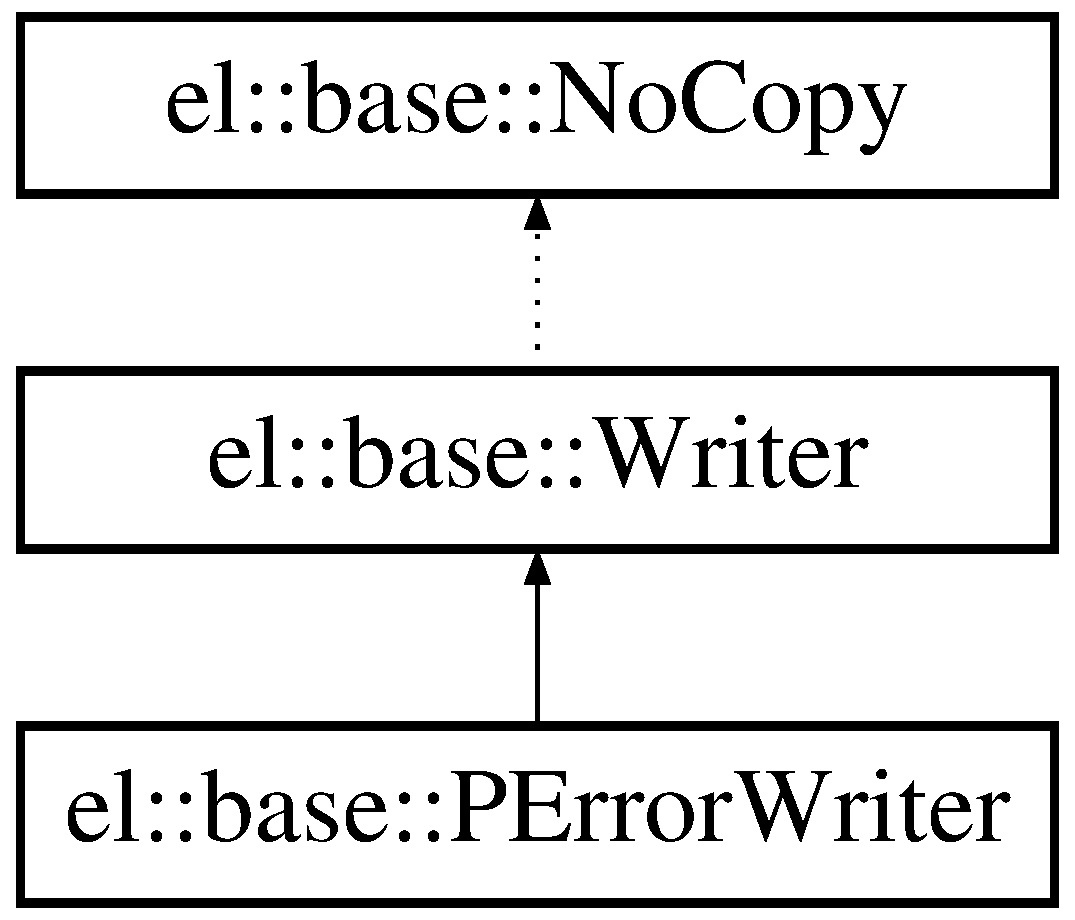
\includegraphics[height=3.000000cm]{classel_1_1base_1_1_p_error_writer}
\end{center}
\end{figure}
\subsection*{Public Member Functions}
\begin{DoxyCompactItemize}
\item 
\hyperlink{classel_1_1base_1_1_p_error_writer_a60d1ff92d16e3927e2c4b5bb77d34092}{P\+Error\+Writer} (\hyperlink{namespaceel_ab0ac6091262344c52dd2d3ad099e8e36}{Level} level, const char $\ast$file, unsigned long int line, const char $\ast$func, \hyperlink{namespaceel_1_1base_a3aa2563d38e47388ba242a1694fc2839}{base\+::\+Dispatch\+Action} dispatch\+Action=\hyperlink{namespaceel_1_1base_a3aa2563d38e47388ba242a1694fc2839a44d8ee68145a7d9849eeaa634c443602}{base\+::\+Dispatch\+Action\+::\+Normal\+Log}, \hyperlink{namespaceel_1_1base_1_1type_a3f79fa74639a13c32f794ba074fe7fb4}{base\+::type\+::\+Verbose\+Level} verbose\+Level=0)
\item 
virtual \hyperlink{classel_1_1base_1_1_p_error_writer_a29754e846334ec7bbf2e780d2f28887f}{$\sim$\+P\+Error\+Writer} (void)
\end{DoxyCompactItemize}
\subsection*{Additional Inherited Members}


\subsection{Detailed Description}


Definition at line 5067 of file easylogging++.\+h.



\subsection{Constructor \& Destructor Documentation}
\hypertarget{classel_1_1base_1_1_p_error_writer_a60d1ff92d16e3927e2c4b5bb77d34092}{}\index{el\+::base\+::\+P\+Error\+Writer@{el\+::base\+::\+P\+Error\+Writer}!P\+Error\+Writer@{P\+Error\+Writer}}
\index{P\+Error\+Writer@{P\+Error\+Writer}!el\+::base\+::\+P\+Error\+Writer@{el\+::base\+::\+P\+Error\+Writer}}
\subsubsection[{P\+Error\+Writer}]{\setlength{\rightskip}{0pt plus 5cm}el\+::base\+::\+P\+Error\+Writer\+::\+P\+Error\+Writer (
\begin{DoxyParamCaption}
\item[{{\bf Level}}]{level, }
\item[{const char $\ast$}]{file, }
\item[{unsigned long int}]{line, }
\item[{const char $\ast$}]{func, }
\item[{{\bf base\+::\+Dispatch\+Action}}]{dispatch\+Action = {\ttfamily {\bf base\+::\+Dispatch\+Action\+::\+Normal\+Log}}, }
\item[{{\bf base\+::type\+::\+Verbose\+Level}}]{verbose\+Level = {\ttfamily 0}}
\end{DoxyParamCaption}
)\hspace{0.3cm}{\ttfamily [inline]}}\label{classel_1_1base_1_1_p_error_writer_a60d1ff92d16e3927e2c4b5bb77d34092}


Definition at line 5069 of file easylogging++.\+h.

\hypertarget{classel_1_1base_1_1_p_error_writer_a29754e846334ec7bbf2e780d2f28887f}{}\index{el\+::base\+::\+P\+Error\+Writer@{el\+::base\+::\+P\+Error\+Writer}!````~P\+Error\+Writer@{$\sim$\+P\+Error\+Writer}}
\index{````~P\+Error\+Writer@{$\sim$\+P\+Error\+Writer}!el\+::base\+::\+P\+Error\+Writer@{el\+::base\+::\+P\+Error\+Writer}}
\subsubsection[{$\sim$\+P\+Error\+Writer}]{\setlength{\rightskip}{0pt plus 5cm}virtual el\+::base\+::\+P\+Error\+Writer\+::$\sim$\+P\+Error\+Writer (
\begin{DoxyParamCaption}
\item[{void}]{}
\end{DoxyParamCaption}
)\hspace{0.3cm}{\ttfamily [inline]}, {\ttfamily [virtual]}}\label{classel_1_1base_1_1_p_error_writer_a29754e846334ec7bbf2e780d2f28887f}


Definition at line 5075 of file easylogging++.\+h.



The documentation for this class was generated from the following file\+:\begin{DoxyCompactItemize}
\item 
lib/\hyperlink{easylogging_09_09_8h}{easylogging++.\+h}\end{DoxyCompactItemize}

\hypertarget{classel_1_1_configuration_1_1_predicate}{}\section{el\+:\+:Configuration\+:\+:Predicate Class Reference}
\label{classel_1_1_configuration_1_1_predicate}\index{el\+::\+Configuration\+::\+Predicate@{el\+::\+Configuration\+::\+Predicate}}


Used to find configuration from configuration (pointers) repository. Avoid using it.  




{\ttfamily \#include $<$easylogging++.\+h$>$}

\subsection*{Public Member Functions}
\begin{DoxyCompactItemize}
\item 
\hyperlink{classel_1_1_configuration_1_1_predicate_ab0a4580d6c2d1aaf36a62913fdc38447}{Predicate} (\hyperlink{namespaceel_ab0ac6091262344c52dd2d3ad099e8e36}{Level} \hyperlink{classel_1_1_configuration_a66a96cf46d20204c50718f8a5e3622e2}{level}, \hyperlink{namespaceel_a281f5db6d6163678bc68a8b23b59e124}{Configuration\+Type} \hyperlink{classel_1_1_configuration_aab5091dcca176e309c0a2268ff55db0d}{configuration\+Type})
\item 
bool \hyperlink{classel_1_1_configuration_1_1_predicate_a985dce44ae06854e789a2ad3be11698f}{operator()} (const \hyperlink{classel_1_1_configuration}{Configuration} $\ast$conf) const 
\end{DoxyCompactItemize}


\subsection{Detailed Description}
Used to find configuration from configuration (pointers) repository. Avoid using it. 

Definition at line 2412 of file easylogging++.\+h.



\subsection{Constructor \& Destructor Documentation}
\hypertarget{classel_1_1_configuration_1_1_predicate_ab0a4580d6c2d1aaf36a62913fdc38447}{}\index{el\+::\+Configuration\+::\+Predicate@{el\+::\+Configuration\+::\+Predicate}!Predicate@{Predicate}}
\index{Predicate@{Predicate}!el\+::\+Configuration\+::\+Predicate@{el\+::\+Configuration\+::\+Predicate}}
\subsubsection[{Predicate}]{\setlength{\rightskip}{0pt plus 5cm}el\+::\+Configuration\+::\+Predicate\+::\+Predicate (
\begin{DoxyParamCaption}
\item[{{\bf Level}}]{level, }
\item[{{\bf Configuration\+Type}}]{configuration\+Type}
\end{DoxyParamCaption}
)\hspace{0.3cm}{\ttfamily [inline]}}\label{classel_1_1_configuration_1_1_predicate_ab0a4580d6c2d1aaf36a62913fdc38447}


Definition at line 2414 of file easylogging++.\+h.



\subsection{Member Function Documentation}
\hypertarget{classel_1_1_configuration_1_1_predicate_a985dce44ae06854e789a2ad3be11698f}{}\index{el\+::\+Configuration\+::\+Predicate@{el\+::\+Configuration\+::\+Predicate}!operator()@{operator()}}
\index{operator()@{operator()}!el\+::\+Configuration\+::\+Predicate@{el\+::\+Configuration\+::\+Predicate}}
\subsubsection[{operator()}]{\setlength{\rightskip}{0pt plus 5cm}bool el\+::\+Configuration\+::\+Predicate\+::operator() (
\begin{DoxyParamCaption}
\item[{const {\bf Configuration} $\ast$}]{conf}
\end{DoxyParamCaption}
) const\hspace{0.3cm}{\ttfamily [inline]}}\label{classel_1_1_configuration_1_1_predicate_a985dce44ae06854e789a2ad3be11698f}


Definition at line 2419 of file easylogging++.\+h.



The documentation for this class was generated from the following file\+:\begin{DoxyCompactItemize}
\item 
lib/\hyperlink{easylogging_09_09_8h}{easylogging++.\+h}\end{DoxyCompactItemize}

\hypertarget{classel_1_1base_1_1_hit_counter_1_1_predicate}{}\section{el\+:\+:base\+:\+:Hit\+Counter\+:\+:Predicate Class Reference}
\label{classel_1_1base_1_1_hit_counter_1_1_predicate}\index{el\+::base\+::\+Hit\+Counter\+::\+Predicate@{el\+::base\+::\+Hit\+Counter\+::\+Predicate}}


{\ttfamily \#include $<$easylogging++.\+h$>$}

\subsection*{Public Member Functions}
\begin{DoxyCompactItemize}
\item 
\hyperlink{classel_1_1base_1_1_hit_counter_1_1_predicate_ab35f4f7da40df5a788c3984d097bb38c}{Predicate} (const char $\ast$\hyperlink{classel_1_1base_1_1_hit_counter_ad04433d214c175775ed61453ead374fc}{filename}, unsigned long int \hyperlink{classel_1_1base_1_1_hit_counter_ab43602346f499854b1764b1c2dcb70dc}{line\+Number})
\item 
bool \hyperlink{classel_1_1base_1_1_hit_counter_1_1_predicate_ae07b1562a3c0ed38457401e60b80b0c5}{operator()} (const \hyperlink{classel_1_1base_1_1_hit_counter}{Hit\+Counter} $\ast$counter)
\end{DoxyCompactItemize}


\subsection{Detailed Description}


Definition at line 3239 of file easylogging++.\+h.



\subsection{Constructor \& Destructor Documentation}
\hypertarget{classel_1_1base_1_1_hit_counter_1_1_predicate_ab35f4f7da40df5a788c3984d097bb38c}{}\index{el\+::base\+::\+Hit\+Counter\+::\+Predicate@{el\+::base\+::\+Hit\+Counter\+::\+Predicate}!Predicate@{Predicate}}
\index{Predicate@{Predicate}!el\+::base\+::\+Hit\+Counter\+::\+Predicate@{el\+::base\+::\+Hit\+Counter\+::\+Predicate}}
\subsubsection[{Predicate}]{\setlength{\rightskip}{0pt plus 5cm}el\+::base\+::\+Hit\+Counter\+::\+Predicate\+::\+Predicate (
\begin{DoxyParamCaption}
\item[{const char $\ast$}]{filename, }
\item[{unsigned long int}]{line\+Number}
\end{DoxyParamCaption}
)\hspace{0.3cm}{\ttfamily [inline]}}\label{classel_1_1base_1_1_hit_counter_1_1_predicate_ab35f4f7da40df5a788c3984d097bb38c}


Definition at line 3241 of file easylogging++.\+h.



\subsection{Member Function Documentation}
\hypertarget{classel_1_1base_1_1_hit_counter_1_1_predicate_ae07b1562a3c0ed38457401e60b80b0c5}{}\index{el\+::base\+::\+Hit\+Counter\+::\+Predicate@{el\+::base\+::\+Hit\+Counter\+::\+Predicate}!operator()@{operator()}}
\index{operator()@{operator()}!el\+::base\+::\+Hit\+Counter\+::\+Predicate@{el\+::base\+::\+Hit\+Counter\+::\+Predicate}}
\subsubsection[{operator()}]{\setlength{\rightskip}{0pt plus 5cm}bool el\+::base\+::\+Hit\+Counter\+::\+Predicate\+::operator() (
\begin{DoxyParamCaption}
\item[{const {\bf Hit\+Counter} $\ast$}]{counter}
\end{DoxyParamCaption}
)\hspace{0.3cm}{\ttfamily [inline]}}\label{classel_1_1base_1_1_hit_counter_1_1_predicate_ae07b1562a3c0ed38457401e60b80b0c5}


Definition at line 3245 of file easylogging++.\+h.



The documentation for this class was generated from the following file\+:\begin{DoxyCompactItemize}
\item 
lib/\hyperlink{easylogging_09_09_8h}{easylogging++.\+h}\end{DoxyCompactItemize}

\hypertarget{classel_1_1base_1_1_registered_hit_counters}{}\section{el\+:\+:base\+:\+:Registered\+Hit\+Counters Class Reference}
\label{classel_1_1base_1_1_registered_hit_counters}\index{el\+::base\+::\+Registered\+Hit\+Counters@{el\+::base\+::\+Registered\+Hit\+Counters}}


Repository for hit counters used across the application.  




{\ttfamily \#include $<$easylogging++.\+h$>$}

Inheritance diagram for el\+:\+:base\+:\+:Registered\+Hit\+Counters\+:\begin{figure}[H]
\begin{center}
\leavevmode
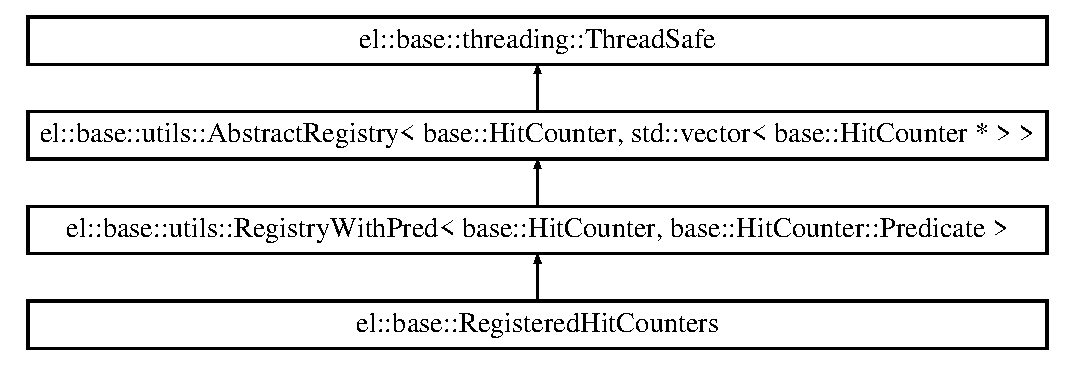
\includegraphics[height=4.000000cm]{classel_1_1base_1_1_registered_hit_counters}
\end{center}
\end{figure}
\subsection*{Public Member Functions}
\begin{DoxyCompactItemize}
\item 
bool \hyperlink{classel_1_1base_1_1_registered_hit_counters_a18fecedc6be778cfd63e30cc42fb9c82}{validate\+Every\+N} (const char $\ast$filename, unsigned long int line\+Number, std\+::size\+\_\+t n)
\begin{DoxyCompactList}\small\item\em Validates counter for every N, i.\+e, registers new if does not exist otherwise updates original one. \end{DoxyCompactList}\item 
bool \hyperlink{classel_1_1base_1_1_registered_hit_counters_af6fa32ffd76776863d8bd2f0e9b341fc}{validate\+After\+N} (const char $\ast$filename, unsigned long int line\+Number, std\+::size\+\_\+t n)
\begin{DoxyCompactList}\small\item\em Validates counter for hits $>$= N, i.\+e, registers new if does not exist otherwise updates original one. \end{DoxyCompactList}\item 
bool \hyperlink{classel_1_1base_1_1_registered_hit_counters_aa270c1b9a8cc3a4d12cea45e07560d98}{validate\+N\+Times} (const char $\ast$filename, unsigned long int line\+Number, std\+::size\+\_\+t n)
\begin{DoxyCompactList}\small\item\em Validates counter for hits are $<$= n, i.\+e, registers new if does not exist otherwise updates original one. \end{DoxyCompactList}\item 
const \hyperlink{classel_1_1base_1_1_hit_counter}{base\+::\+Hit\+Counter} $\ast$ \hyperlink{classel_1_1base_1_1_registered_hit_counters_a0ca8cd04da5686048644e8cc1533b561}{get\+Counter} (const char $\ast$filename, unsigned long int line\+Number)
\begin{DoxyCompactList}\small\item\em Gets hit counter registered at specified position. \end{DoxyCompactList}\end{DoxyCompactItemize}
\subsection*{Additional Inherited Members}


\subsection{Detailed Description}
Repository for hit counters used across the application. 

Definition at line 3262 of file easylogging++.\+h.



\subsection{Member Function Documentation}
\hypertarget{classel_1_1base_1_1_registered_hit_counters_a0ca8cd04da5686048644e8cc1533b561}{}\index{el\+::base\+::\+Registered\+Hit\+Counters@{el\+::base\+::\+Registered\+Hit\+Counters}!get\+Counter@{get\+Counter}}
\index{get\+Counter@{get\+Counter}!el\+::base\+::\+Registered\+Hit\+Counters@{el\+::base\+::\+Registered\+Hit\+Counters}}
\subsubsection[{get\+Counter}]{\setlength{\rightskip}{0pt plus 5cm}const {\bf base\+::\+Hit\+Counter}$\ast$ el\+::base\+::\+Registered\+Hit\+Counters\+::get\+Counter (
\begin{DoxyParamCaption}
\item[{const char $\ast$}]{filename, }
\item[{unsigned long int}]{line\+Number}
\end{DoxyParamCaption}
)\hspace{0.3cm}{\ttfamily [inline]}}\label{classel_1_1base_1_1_registered_hit_counters_a0ca8cd04da5686048644e8cc1533b561}


Gets hit counter registered at specified position. 



Definition at line 3310 of file easylogging++.\+h.

\hypertarget{classel_1_1base_1_1_registered_hit_counters_af6fa32ffd76776863d8bd2f0e9b341fc}{}\index{el\+::base\+::\+Registered\+Hit\+Counters@{el\+::base\+::\+Registered\+Hit\+Counters}!validate\+After\+N@{validate\+After\+N}}
\index{validate\+After\+N@{validate\+After\+N}!el\+::base\+::\+Registered\+Hit\+Counters@{el\+::base\+::\+Registered\+Hit\+Counters}}
\subsubsection[{validate\+After\+N}]{\setlength{\rightskip}{0pt plus 5cm}bool el\+::base\+::\+Registered\+Hit\+Counters\+::validate\+After\+N (
\begin{DoxyParamCaption}
\item[{const char $\ast$}]{filename, }
\item[{unsigned long int}]{line\+Number, }
\item[{std\+::size\+\_\+t}]{n}
\end{DoxyParamCaption}
)\hspace{0.3cm}{\ttfamily [inline]}}\label{classel_1_1base_1_1_registered_hit_counters_af6fa32ffd76776863d8bd2f0e9b341fc}


Validates counter for hits $>$= N, i.\+e, registers new if does not exist otherwise updates original one. 

\begin{DoxyReturn}{Returns}
True if validation resulted in triggering hit. Meaning logs should be written everytime true is returned 
\end{DoxyReturn}


Definition at line 3279 of file easylogging++.\+h.

\hypertarget{classel_1_1base_1_1_registered_hit_counters_a18fecedc6be778cfd63e30cc42fb9c82}{}\index{el\+::base\+::\+Registered\+Hit\+Counters@{el\+::base\+::\+Registered\+Hit\+Counters}!validate\+Every\+N@{validate\+Every\+N}}
\index{validate\+Every\+N@{validate\+Every\+N}!el\+::base\+::\+Registered\+Hit\+Counters@{el\+::base\+::\+Registered\+Hit\+Counters}}
\subsubsection[{validate\+Every\+N}]{\setlength{\rightskip}{0pt plus 5cm}bool el\+::base\+::\+Registered\+Hit\+Counters\+::validate\+Every\+N (
\begin{DoxyParamCaption}
\item[{const char $\ast$}]{filename, }
\item[{unsigned long int}]{line\+Number, }
\item[{std\+::size\+\_\+t}]{n}
\end{DoxyParamCaption}
)\hspace{0.3cm}{\ttfamily [inline]}}\label{classel_1_1base_1_1_registered_hit_counters_a18fecedc6be778cfd63e30cc42fb9c82}


Validates counter for every N, i.\+e, registers new if does not exist otherwise updates original one. 

\begin{DoxyReturn}{Returns}
True if validation resulted in triggering hit. Meaning logs should be written everytime true is returned 
\end{DoxyReturn}


Definition at line 3266 of file easylogging++.\+h.

\hypertarget{classel_1_1base_1_1_registered_hit_counters_aa270c1b9a8cc3a4d12cea45e07560d98}{}\index{el\+::base\+::\+Registered\+Hit\+Counters@{el\+::base\+::\+Registered\+Hit\+Counters}!validate\+N\+Times@{validate\+N\+Times}}
\index{validate\+N\+Times@{validate\+N\+Times}!el\+::base\+::\+Registered\+Hit\+Counters@{el\+::base\+::\+Registered\+Hit\+Counters}}
\subsubsection[{validate\+N\+Times}]{\setlength{\rightskip}{0pt plus 5cm}bool el\+::base\+::\+Registered\+Hit\+Counters\+::validate\+N\+Times (
\begin{DoxyParamCaption}
\item[{const char $\ast$}]{filename, }
\item[{unsigned long int}]{line\+Number, }
\item[{std\+::size\+\_\+t}]{n}
\end{DoxyParamCaption}
)\hspace{0.3cm}{\ttfamily [inline]}}\label{classel_1_1base_1_1_registered_hit_counters_aa270c1b9a8cc3a4d12cea45e07560d98}


Validates counter for hits are $<$= n, i.\+e, registers new if does not exist otherwise updates original one. 

\begin{DoxyReturn}{Returns}
True if validation resulted in triggering hit. Meaning logs should be written everytime true is returned 
\end{DoxyReturn}


Definition at line 3296 of file easylogging++.\+h.



The documentation for this class was generated from the following file\+:\begin{DoxyCompactItemize}
\item 
lib/\hyperlink{easylogging_09_09_8h}{easylogging++.\+h}\end{DoxyCompactItemize}

\hypertarget{classel_1_1base_1_1_registered_loggers}{}\section{el\+:\+:base\+:\+:Registered\+Loggers Class Reference}
\label{classel_1_1base_1_1_registered_loggers}\index{el\+::base\+::\+Registered\+Loggers@{el\+::base\+::\+Registered\+Loggers}}


\hyperlink{classel_1_1_loggers}{Loggers} repository.  




{\ttfamily \#include $<$easylogging++.\+h$>$}

Inheritance diagram for el\+:\+:base\+:\+:Registered\+Loggers\+:\begin{figure}[H]
\begin{center}
\leavevmode
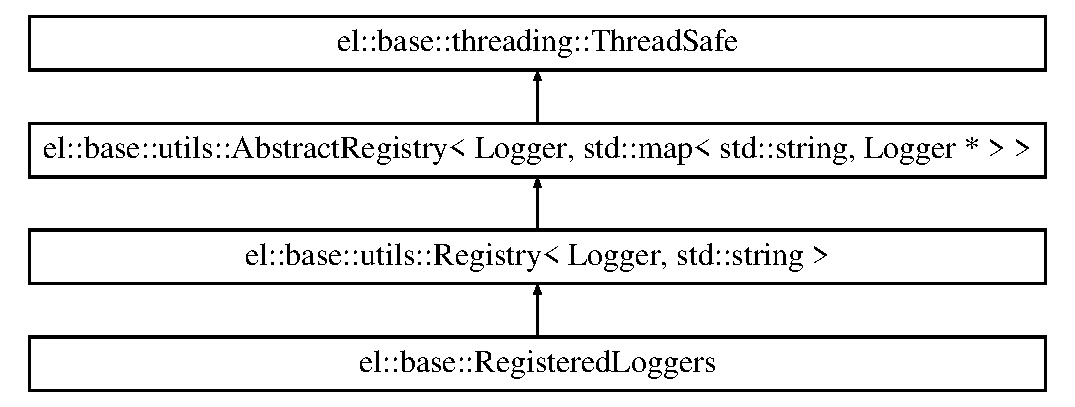
\includegraphics[height=4.000000cm]{classel_1_1base_1_1_registered_loggers}
\end{center}
\end{figure}
\subsection*{Public Member Functions}
\begin{DoxyCompactItemize}
\item 
\hyperlink{classel_1_1base_1_1_registered_loggers_ae52ec336770d33fef86f234e4e68dce5}{Registered\+Loggers} (const \hyperlink{namespaceel_ad4c4b2f7d70a4b02568a9f70724a6b39}{Log\+Builder\+Ptr} \&default\+Log\+Builder)
\item 
virtual \hyperlink{classel_1_1base_1_1_registered_loggers_ac87ee24f4d1bb36757f6ce1e1f5a8362}{$\sim$\+Registered\+Loggers} (void)
\item 
void \hyperlink{classel_1_1base_1_1_registered_loggers_a28e1f955ad55d89a4ae91fa74545ee4f}{set\+Default\+Configurations} (const \hyperlink{classel_1_1_configurations}{Configurations} \&configurations)
\item 
\hyperlink{classel_1_1_configurations}{Configurations} $\ast$ \hyperlink{classel_1_1base_1_1_registered_loggers_acb38f67cf5e297f4be3efa5312e09914}{default\+Configurations} (void)
\item 
\hyperlink{classel_1_1_logger}{Logger} $\ast$ \hyperlink{classel_1_1base_1_1_registered_loggers_a8e554505cd7f66d31e91933b61d74144}{get} (const std\+::string \&id, bool force\+Creation=true)
\item 
bool \hyperlink{classel_1_1base_1_1_registered_loggers_a4d17dc9673f6aa6216571e182097400a}{remove} (const std\+::string \&id)
\item 
bool \hyperlink{classel_1_1base_1_1_registered_loggers_a85916925e2c53d1ebf9865625132a0be}{has} (const std\+::string \&id)
\item 
void \hyperlink{classel_1_1base_1_1_registered_loggers_ad8fa8f829fdb6a03e6f5a38704811e7b}{unregister} (\hyperlink{classel_1_1_logger}{Logger} $\ast$\&logger)
\item 
\hyperlink{namespaceel_1_1base_af7602da9fe1d6c75985184fb0e39fd11}{base\+::\+Log\+Streams\+Reference\+Map} $\ast$ \hyperlink{classel_1_1base_1_1_registered_loggers_a11eb24bac74b7ae2d85b324fed707819}{log\+Streams\+Reference} (void)
\item 
void \hyperlink{classel_1_1base_1_1_registered_loggers_abe6fdac67d9d4c35fb48c9fd88a49c2e}{flush\+All} (void)
\end{DoxyCompactItemize}
\subsection*{Friends}
\begin{DoxyCompactItemize}
\item 
class \hyperlink{classel_1_1base_1_1_registered_loggers_acc1efd1b8a3fc5e0028dab98b02e550a}{el\+::base\+::\+Storage}
\end{DoxyCompactItemize}
\subsection*{Additional Inherited Members}


\subsection{Detailed Description}
\hyperlink{classel_1_1_loggers}{Loggers} repository. 

Definition at line 3603 of file easylogging++.\+h.



\subsection{Constructor \& Destructor Documentation}
\hypertarget{classel_1_1base_1_1_registered_loggers_ae52ec336770d33fef86f234e4e68dce5}{}\index{el\+::base\+::\+Registered\+Loggers@{el\+::base\+::\+Registered\+Loggers}!Registered\+Loggers@{Registered\+Loggers}}
\index{Registered\+Loggers@{Registered\+Loggers}!el\+::base\+::\+Registered\+Loggers@{el\+::base\+::\+Registered\+Loggers}}
\subsubsection[{Registered\+Loggers}]{\setlength{\rightskip}{0pt plus 5cm}el\+::base\+::\+Registered\+Loggers\+::\+Registered\+Loggers (
\begin{DoxyParamCaption}
\item[{const {\bf Log\+Builder\+Ptr} \&}]{default\+Log\+Builder}
\end{DoxyParamCaption}
)\hspace{0.3cm}{\ttfamily [inline]}, {\ttfamily [explicit]}}\label{classel_1_1base_1_1_registered_loggers_ae52ec336770d33fef86f234e4e68dce5}


Definition at line 3605 of file easylogging++.\+h.

\hypertarget{classel_1_1base_1_1_registered_loggers_ac87ee24f4d1bb36757f6ce1e1f5a8362}{}\index{el\+::base\+::\+Registered\+Loggers@{el\+::base\+::\+Registered\+Loggers}!````~Registered\+Loggers@{$\sim$\+Registered\+Loggers}}
\index{````~Registered\+Loggers@{$\sim$\+Registered\+Loggers}!el\+::base\+::\+Registered\+Loggers@{el\+::base\+::\+Registered\+Loggers}}
\subsubsection[{$\sim$\+Registered\+Loggers}]{\setlength{\rightskip}{0pt plus 5cm}virtual el\+::base\+::\+Registered\+Loggers\+::$\sim$\+Registered\+Loggers (
\begin{DoxyParamCaption}
\item[{void}]{}
\end{DoxyParamCaption}
)\hspace{0.3cm}{\ttfamily [inline]}, {\ttfamily [virtual]}}\label{classel_1_1base_1_1_registered_loggers_ac87ee24f4d1bb36757f6ce1e1f5a8362}


Definition at line 3610 of file easylogging++.\+h.



\subsection{Member Function Documentation}
\hypertarget{classel_1_1base_1_1_registered_loggers_acb38f67cf5e297f4be3efa5312e09914}{}\index{el\+::base\+::\+Registered\+Loggers@{el\+::base\+::\+Registered\+Loggers}!default\+Configurations@{default\+Configurations}}
\index{default\+Configurations@{default\+Configurations}!el\+::base\+::\+Registered\+Loggers@{el\+::base\+::\+Registered\+Loggers}}
\subsubsection[{default\+Configurations}]{\setlength{\rightskip}{0pt plus 5cm}{\bf Configurations}$\ast$ el\+::base\+::\+Registered\+Loggers\+::default\+Configurations (
\begin{DoxyParamCaption}
\item[{void}]{}
\end{DoxyParamCaption}
)\hspace{0.3cm}{\ttfamily [inline]}}\label{classel_1_1base_1_1_registered_loggers_acb38f67cf5e297f4be3efa5312e09914}


Definition at line 3619 of file easylogging++.\+h.

\hypertarget{classel_1_1base_1_1_registered_loggers_abe6fdac67d9d4c35fb48c9fd88a49c2e}{}\index{el\+::base\+::\+Registered\+Loggers@{el\+::base\+::\+Registered\+Loggers}!flush\+All@{flush\+All}}
\index{flush\+All@{flush\+All}!el\+::base\+::\+Registered\+Loggers@{el\+::base\+::\+Registered\+Loggers}}
\subsubsection[{flush\+All}]{\setlength{\rightskip}{0pt plus 5cm}void el\+::base\+::\+Registered\+Loggers\+::flush\+All (
\begin{DoxyParamCaption}
\item[{void}]{}
\end{DoxyParamCaption}
)\hspace{0.3cm}{\ttfamily [inline]}}\label{classel_1_1base_1_1_registered_loggers_abe6fdac67d9d4c35fb48c9fd88a49c2e}


Definition at line 3663 of file easylogging++.\+h.

\hypertarget{classel_1_1base_1_1_registered_loggers_a8e554505cd7f66d31e91933b61d74144}{}\index{el\+::base\+::\+Registered\+Loggers@{el\+::base\+::\+Registered\+Loggers}!get@{get}}
\index{get@{get}!el\+::base\+::\+Registered\+Loggers@{el\+::base\+::\+Registered\+Loggers}}
\subsubsection[{get}]{\setlength{\rightskip}{0pt plus 5cm}{\bf Logger}$\ast$ el\+::base\+::\+Registered\+Loggers\+::get (
\begin{DoxyParamCaption}
\item[{const std\+::string \&}]{id, }
\item[{bool}]{force\+Creation = {\ttfamily true}}
\end{DoxyParamCaption}
)\hspace{0.3cm}{\ttfamily [inline]}}\label{classel_1_1base_1_1_registered_loggers_a8e554505cd7f66d31e91933b61d74144}


Definition at line 3623 of file easylogging++.\+h.

\hypertarget{classel_1_1base_1_1_registered_loggers_a85916925e2c53d1ebf9865625132a0be}{}\index{el\+::base\+::\+Registered\+Loggers@{el\+::base\+::\+Registered\+Loggers}!has@{has}}
\index{has@{has}!el\+::base\+::\+Registered\+Loggers@{el\+::base\+::\+Registered\+Loggers}}
\subsubsection[{has}]{\setlength{\rightskip}{0pt plus 5cm}bool el\+::base\+::\+Registered\+Loggers\+::has (
\begin{DoxyParamCaption}
\item[{const std\+::string \&}]{id}
\end{DoxyParamCaption}
)\hspace{0.3cm}{\ttfamily [inline]}}\label{classel_1_1base_1_1_registered_loggers_a85916925e2c53d1ebf9865625132a0be}


Definition at line 3650 of file easylogging++.\+h.

\hypertarget{classel_1_1base_1_1_registered_loggers_a11eb24bac74b7ae2d85b324fed707819}{}\index{el\+::base\+::\+Registered\+Loggers@{el\+::base\+::\+Registered\+Loggers}!log\+Streams\+Reference@{log\+Streams\+Reference}}
\index{log\+Streams\+Reference@{log\+Streams\+Reference}!el\+::base\+::\+Registered\+Loggers@{el\+::base\+::\+Registered\+Loggers}}
\subsubsection[{log\+Streams\+Reference}]{\setlength{\rightskip}{0pt plus 5cm}{\bf base\+::\+Log\+Streams\+Reference\+Map}$\ast$ el\+::base\+::\+Registered\+Loggers\+::log\+Streams\+Reference (
\begin{DoxyParamCaption}
\item[{void}]{}
\end{DoxyParamCaption}
)\hspace{0.3cm}{\ttfamily [inline]}}\label{classel_1_1base_1_1_registered_loggers_a11eb24bac74b7ae2d85b324fed707819}


Definition at line 3659 of file easylogging++.\+h.

\hypertarget{classel_1_1base_1_1_registered_loggers_a4d17dc9673f6aa6216571e182097400a}{}\index{el\+::base\+::\+Registered\+Loggers@{el\+::base\+::\+Registered\+Loggers}!remove@{remove}}
\index{remove@{remove}!el\+::base\+::\+Registered\+Loggers@{el\+::base\+::\+Registered\+Loggers}}
\subsubsection[{remove}]{\setlength{\rightskip}{0pt plus 5cm}bool el\+::base\+::\+Registered\+Loggers\+::remove (
\begin{DoxyParamCaption}
\item[{const std\+::string \&}]{id}
\end{DoxyParamCaption}
)\hspace{0.3cm}{\ttfamily [inline]}}\label{classel_1_1base_1_1_registered_loggers_a4d17dc9673f6aa6216571e182097400a}


Definition at line 3639 of file easylogging++.\+h.

\hypertarget{classel_1_1base_1_1_registered_loggers_a28e1f955ad55d89a4ae91fa74545ee4f}{}\index{el\+::base\+::\+Registered\+Loggers@{el\+::base\+::\+Registered\+Loggers}!set\+Default\+Configurations@{set\+Default\+Configurations}}
\index{set\+Default\+Configurations@{set\+Default\+Configurations}!el\+::base\+::\+Registered\+Loggers@{el\+::base\+::\+Registered\+Loggers}}
\subsubsection[{set\+Default\+Configurations}]{\setlength{\rightskip}{0pt plus 5cm}void el\+::base\+::\+Registered\+Loggers\+::set\+Default\+Configurations (
\begin{DoxyParamCaption}
\item[{const {\bf Configurations} \&}]{configurations}
\end{DoxyParamCaption}
)\hspace{0.3cm}{\ttfamily [inline]}}\label{classel_1_1base_1_1_registered_loggers_a28e1f955ad55d89a4ae91fa74545ee4f}


Definition at line 3614 of file easylogging++.\+h.

\hypertarget{classel_1_1base_1_1_registered_loggers_ad8fa8f829fdb6a03e6f5a38704811e7b}{}\index{el\+::base\+::\+Registered\+Loggers@{el\+::base\+::\+Registered\+Loggers}!unregister@{unregister}}
\index{unregister@{unregister}!el\+::base\+::\+Registered\+Loggers@{el\+::base\+::\+Registered\+Loggers}}
\subsubsection[{unregister}]{\setlength{\rightskip}{0pt plus 5cm}void el\+::base\+::\+Registered\+Loggers\+::unregister (
\begin{DoxyParamCaption}
\item[{{\bf Logger} $\ast$\&}]{logger}
\end{DoxyParamCaption}
)\hspace{0.3cm}{\ttfamily [inline]}}\label{classel_1_1base_1_1_registered_loggers_ad8fa8f829fdb6a03e6f5a38704811e7b}


Definition at line 3654 of file easylogging++.\+h.



\subsection{Friends And Related Function Documentation}
\hypertarget{classel_1_1base_1_1_registered_loggers_acc1efd1b8a3fc5e0028dab98b02e550a}{}\index{el\+::base\+::\+Registered\+Loggers@{el\+::base\+::\+Registered\+Loggers}!el\+::base\+::\+Storage@{el\+::base\+::\+Storage}}
\index{el\+::base\+::\+Storage@{el\+::base\+::\+Storage}!el\+::base\+::\+Registered\+Loggers@{el\+::base\+::\+Registered\+Loggers}}
\subsubsection[{el\+::base\+::\+Storage}]{\setlength{\rightskip}{0pt plus 5cm}friend class {\bf el\+::base\+::\+Storage}\hspace{0.3cm}{\ttfamily [friend]}}\label{classel_1_1base_1_1_registered_loggers_acc1efd1b8a3fc5e0028dab98b02e550a}


Definition at line 3677 of file easylogging++.\+h.



The documentation for this class was generated from the following file\+:\begin{DoxyCompactItemize}
\item 
lib/\hyperlink{easylogging_09_09_8h}{easylogging++.\+h}\end{DoxyCompactItemize}

\hypertarget{classel_1_1base_1_1utils_1_1_registry}{}\section{el\+:\+:base\+:\+:utils\+:\+:Registry$<$ T\+\_\+\+Ptr, T\+\_\+\+Key $>$ Class Template Reference}
\label{classel_1_1base_1_1utils_1_1_registry}\index{el\+::base\+::utils\+::\+Registry$<$ T\+\_\+\+Ptr, T\+\_\+\+Key $>$@{el\+::base\+::utils\+::\+Registry$<$ T\+\_\+\+Ptr, T\+\_\+\+Key $>$}}


A pointer registry mechanism to manage memory and provide search functionalities. (non-\/predicate version)  




{\ttfamily \#include $<$easylogging++.\+h$>$}

Inheritance diagram for el\+:\+:base\+:\+:utils\+:\+:Registry$<$ T\+\_\+\+Ptr, T\+\_\+\+Key $>$\+:\begin{figure}[H]
\begin{center}
\leavevmode
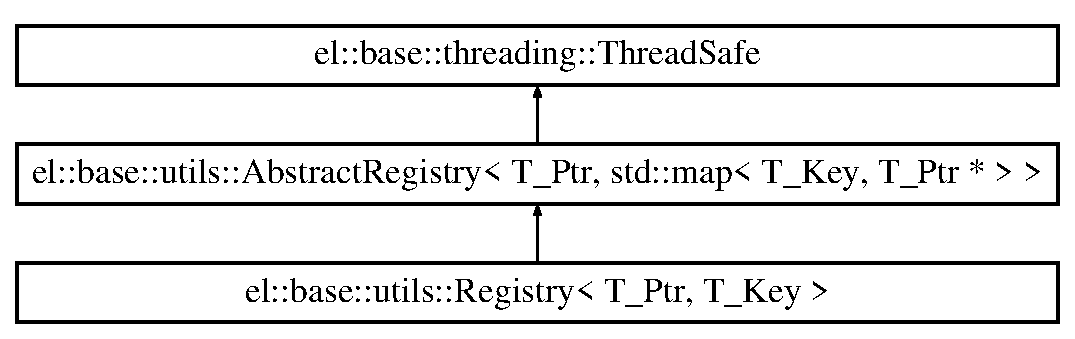
\includegraphics[height=3.000000cm]{classel_1_1base_1_1utils_1_1_registry}
\end{center}
\end{figure}
\subsection*{Public Types}
\begin{DoxyCompactItemize}
\item 
typedef \hyperlink{classel_1_1base_1_1utils_1_1_registry}{Registry}$<$ T\+\_\+\+Ptr, T\+\_\+\+Key $>$\+::\hyperlink{classel_1_1base_1_1utils_1_1_registry_a31f3d725285e6b65f1f9e990066f96ed}{iterator} \hyperlink{classel_1_1base_1_1utils_1_1_registry_a31f3d725285e6b65f1f9e990066f96ed}{iterator}
\item 
typedef \hyperlink{classel_1_1base_1_1utils_1_1_registry}{Registry}$<$ T\+\_\+\+Ptr, T\+\_\+\+Key $>$\+::\hyperlink{classel_1_1base_1_1utils_1_1_registry_a955e62adc74c60d0205b52a3fc430cef}{const\+\_\+iterator} \hyperlink{classel_1_1base_1_1utils_1_1_registry_a955e62adc74c60d0205b52a3fc430cef}{const\+\_\+iterator}
\end{DoxyCompactItemize}
\subsection*{Public Member Functions}
\begin{DoxyCompactItemize}
\item 
\hyperlink{classel_1_1base_1_1utils_1_1_registry_aa4bb56a1aff481cc6cf8979b2f2c6eca}{Registry} (void)
\item 
\hyperlink{classel_1_1base_1_1utils_1_1_registry_adf5e97aa801be3b93e116ad645304759}{Registry} (const \hyperlink{classel_1_1base_1_1utils_1_1_registry}{Registry} \&sr)
\begin{DoxyCompactList}\small\item\em Copy constructor that is useful for base classes. Try to avoid this constructor, use move constructor. \end{DoxyCompactList}\item 
\hyperlink{classel_1_1base_1_1utils_1_1_registry}{Registry} \& \hyperlink{classel_1_1base_1_1utils_1_1_registry_a80e0ce12b7d0c24462b385fc7b3149e0}{operator=} (const \hyperlink{classel_1_1base_1_1utils_1_1_registry}{Registry} \&sr)
\begin{DoxyCompactList}\small\item\em Assignment operator that unregisters all the existing registeries and deeply copies each of repo element. \end{DoxyCompactList}\item 
virtual \hyperlink{classel_1_1base_1_1utils_1_1_registry_a79aa9dfa385e233bf619d44422f4992c}{$\sim$\+Registry} (void)
\end{DoxyCompactItemize}
\subsection*{Protected Member Functions}
\begin{DoxyCompactItemize}
\item 
virtual void \hyperlink{classel_1_1base_1_1utils_1_1_registry_ac40e62ddf5017beb91c28b472c9628c2}{unregister\+All} (void) \hyperlink{easylogging_09_09_8h_a2f812449f8d3355cf5b03ceb2ee5021b}{E\+L\+P\+P\+\_\+\+F\+I\+N\+A\+L}
\begin{DoxyCompactList}\small\item\em Unregisters all the pointers from current repository. \end{DoxyCompactList}\item 
virtual void \hyperlink{classel_1_1base_1_1utils_1_1_registry_ab10b3dd25ff0df036e7a015635a15dee}{register\+New} (const T\+\_\+\+Key \&uniq\+Key, T\+\_\+\+Ptr $\ast$ptr) \hyperlink{easylogging_09_09_8h_a2f812449f8d3355cf5b03ceb2ee5021b}{E\+L\+P\+P\+\_\+\+F\+I\+N\+A\+L}
\begin{DoxyCompactList}\small\item\em Registers new registry to repository. \end{DoxyCompactList}\item 
void \hyperlink{classel_1_1base_1_1utils_1_1_registry_aab6f0ce3a99feff11add0bd8b869fcb8}{unregister} (const T\+\_\+\+Key \&uniq\+Key)
\begin{DoxyCompactList}\small\item\em Unregisters single entry mapped to specified unique key. \end{DoxyCompactList}\item 
T\+\_\+\+Ptr $\ast$ \hyperlink{classel_1_1base_1_1utils_1_1_registry_a18c332267f2acbe78c97a611dec2e5c2}{get} (const T\+\_\+\+Key \&uniq\+Key)
\begin{DoxyCompactList}\small\item\em Gets pointer from repository. If none found, nullptr is returned. \end{DoxyCompactList}\end{DoxyCompactItemize}


\subsection{Detailed Description}
\subsubsection*{template$<$typename T\+\_\+\+Ptr, typename T\+\_\+\+Key = const char$\ast$$>$class el\+::base\+::utils\+::\+Registry$<$ T\+\_\+\+Ptr, T\+\_\+\+Key $>$}

A pointer registry mechanism to manage memory and provide search functionalities. (non-\/predicate version) 

N\+O\+T\+E\+: This is thread-\/unsafe implementation (although it contains lock function, it does not use these functions) of Abstract\+Registry$<$\+T\+\_\+\+Ptr, Container$>$. Any implementation of this class should be explicitly (by using lock functions) 

Definition at line 1929 of file easylogging++.\+h.



\subsection{Member Typedef Documentation}
\hypertarget{classel_1_1base_1_1utils_1_1_registry_a955e62adc74c60d0205b52a3fc430cef}{}\index{el\+::base\+::utils\+::\+Registry@{el\+::base\+::utils\+::\+Registry}!const\+\_\+iterator@{const\+\_\+iterator}}
\index{const\+\_\+iterator@{const\+\_\+iterator}!el\+::base\+::utils\+::\+Registry@{el\+::base\+::utils\+::\+Registry}}
\subsubsection[{const\+\_\+iterator}]{\setlength{\rightskip}{0pt plus 5cm}template$<$typename T\+\_\+\+Ptr, typename T\+\_\+\+Key = const char$\ast$$>$ typedef {\bf Registry}$<$T\+\_\+\+Ptr, T\+\_\+\+Key$>$\+::{\bf const\+\_\+iterator} {\bf el\+::base\+::utils\+::\+Registry}$<$ T\+\_\+\+Ptr, T\+\_\+\+Key $>$\+::{\bf const\+\_\+iterator}}\label{classel_1_1base_1_1utils_1_1_registry_a955e62adc74c60d0205b52a3fc430cef}


Definition at line 1932 of file easylogging++.\+h.

\hypertarget{classel_1_1base_1_1utils_1_1_registry_a31f3d725285e6b65f1f9e990066f96ed}{}\index{el\+::base\+::utils\+::\+Registry@{el\+::base\+::utils\+::\+Registry}!iterator@{iterator}}
\index{iterator@{iterator}!el\+::base\+::utils\+::\+Registry@{el\+::base\+::utils\+::\+Registry}}
\subsubsection[{iterator}]{\setlength{\rightskip}{0pt plus 5cm}template$<$typename T\+\_\+\+Ptr, typename T\+\_\+\+Key = const char$\ast$$>$ typedef {\bf Registry}$<$T\+\_\+\+Ptr, T\+\_\+\+Key$>$\+::{\bf iterator} {\bf el\+::base\+::utils\+::\+Registry}$<$ T\+\_\+\+Ptr, T\+\_\+\+Key $>$\+::{\bf iterator}}\label{classel_1_1base_1_1utils_1_1_registry_a31f3d725285e6b65f1f9e990066f96ed}


Definition at line 1931 of file easylogging++.\+h.



\subsection{Constructor \& Destructor Documentation}
\hypertarget{classel_1_1base_1_1utils_1_1_registry_aa4bb56a1aff481cc6cf8979b2f2c6eca}{}\index{el\+::base\+::utils\+::\+Registry@{el\+::base\+::utils\+::\+Registry}!Registry@{Registry}}
\index{Registry@{Registry}!el\+::base\+::utils\+::\+Registry@{el\+::base\+::utils\+::\+Registry}}
\subsubsection[{Registry}]{\setlength{\rightskip}{0pt plus 5cm}template$<$typename T\+\_\+\+Ptr, typename T\+\_\+\+Key = const char$\ast$$>$ {\bf el\+::base\+::utils\+::\+Registry}$<$ T\+\_\+\+Ptr, T\+\_\+\+Key $>$\+::{\bf Registry} (
\begin{DoxyParamCaption}
\item[{void}]{}
\end{DoxyParamCaption}
)\hspace{0.3cm}{\ttfamily [inline]}}\label{classel_1_1base_1_1utils_1_1_registry_aa4bb56a1aff481cc6cf8979b2f2c6eca}


Definition at line 1934 of file easylogging++.\+h.

\hypertarget{classel_1_1base_1_1utils_1_1_registry_adf5e97aa801be3b93e116ad645304759}{}\index{el\+::base\+::utils\+::\+Registry@{el\+::base\+::utils\+::\+Registry}!Registry@{Registry}}
\index{Registry@{Registry}!el\+::base\+::utils\+::\+Registry@{el\+::base\+::utils\+::\+Registry}}
\subsubsection[{Registry}]{\setlength{\rightskip}{0pt plus 5cm}template$<$typename T\+\_\+\+Ptr, typename T\+\_\+\+Key = const char$\ast$$>$ {\bf el\+::base\+::utils\+::\+Registry}$<$ T\+\_\+\+Ptr, T\+\_\+\+Key $>$\+::{\bf Registry} (
\begin{DoxyParamCaption}
\item[{const {\bf Registry}$<$ T\+\_\+\+Ptr, T\+\_\+\+Key $>$ \&}]{sr}
\end{DoxyParamCaption}
)\hspace{0.3cm}{\ttfamily [inline]}}\label{classel_1_1base_1_1utils_1_1_registry_adf5e97aa801be3b93e116ad645304759}


Copy constructor that is useful for base classes. Try to avoid this constructor, use move constructor. 



Definition at line 1937 of file easylogging++.\+h.

\hypertarget{classel_1_1base_1_1utils_1_1_registry_a79aa9dfa385e233bf619d44422f4992c}{}\index{el\+::base\+::utils\+::\+Registry@{el\+::base\+::utils\+::\+Registry}!````~Registry@{$\sim$\+Registry}}
\index{````~Registry@{$\sim$\+Registry}!el\+::base\+::utils\+::\+Registry@{el\+::base\+::utils\+::\+Registry}}
\subsubsection[{$\sim$\+Registry}]{\setlength{\rightskip}{0pt plus 5cm}template$<$typename T\+\_\+\+Ptr, typename T\+\_\+\+Key = const char$\ast$$>$ virtual {\bf el\+::base\+::utils\+::\+Registry}$<$ T\+\_\+\+Ptr, T\+\_\+\+Key $>$\+::$\sim${\bf Registry} (
\begin{DoxyParamCaption}
\item[{void}]{}
\end{DoxyParamCaption}
)\hspace{0.3cm}{\ttfamily [inline]}, {\ttfamily [virtual]}}\label{classel_1_1base_1_1utils_1_1_registry_a79aa9dfa385e233bf619d44422f4992c}


Definition at line 1955 of file easylogging++.\+h.



\subsection{Member Function Documentation}
\hypertarget{classel_1_1base_1_1utils_1_1_registry_a18c332267f2acbe78c97a611dec2e5c2}{}\index{el\+::base\+::utils\+::\+Registry@{el\+::base\+::utils\+::\+Registry}!get@{get}}
\index{get@{get}!el\+::base\+::utils\+::\+Registry@{el\+::base\+::utils\+::\+Registry}}
\subsubsection[{get}]{\setlength{\rightskip}{0pt plus 5cm}template$<$typename T\+\_\+\+Ptr, typename T\+\_\+\+Key = const char$\ast$$>$ T\+\_\+\+Ptr$\ast$ {\bf el\+::base\+::utils\+::\+Registry}$<$ T\+\_\+\+Ptr, T\+\_\+\+Key $>$\+::get (
\begin{DoxyParamCaption}
\item[{const T\+\_\+\+Key \&}]{uniq\+Key}
\end{DoxyParamCaption}
)\hspace{0.3cm}{\ttfamily [inline]}, {\ttfamily [protected]}}\label{classel_1_1base_1_1utils_1_1_registry_a18c332267f2acbe78c97a611dec2e5c2}


Gets pointer from repository. If none found, nullptr is returned. 



Definition at line 1985 of file easylogging++.\+h.

\hypertarget{classel_1_1base_1_1utils_1_1_registry_a80e0ce12b7d0c24462b385fc7b3149e0}{}\index{el\+::base\+::utils\+::\+Registry@{el\+::base\+::utils\+::\+Registry}!operator=@{operator=}}
\index{operator=@{operator=}!el\+::base\+::utils\+::\+Registry@{el\+::base\+::utils\+::\+Registry}}
\subsubsection[{operator=}]{\setlength{\rightskip}{0pt plus 5cm}template$<$typename T\+\_\+\+Ptr, typename T\+\_\+\+Key = const char$\ast$$>$ {\bf Registry}\& {\bf el\+::base\+::utils\+::\+Registry}$<$ T\+\_\+\+Ptr, T\+\_\+\+Key $>$\+::operator= (
\begin{DoxyParamCaption}
\item[{const {\bf Registry}$<$ T\+\_\+\+Ptr, T\+\_\+\+Key $>$ \&}]{sr}
\end{DoxyParamCaption}
)\hspace{0.3cm}{\ttfamily [inline]}}\label{classel_1_1base_1_1utils_1_1_registry_a80e0ce12b7d0c24462b385fc7b3149e0}


Assignment operator that unregisters all the existing registeries and deeply copies each of repo element. 

\begin{DoxySeeAlso}{See also}
\hyperlink{classel_1_1base_1_1utils_1_1_registry_ac40e62ddf5017beb91c28b472c9628c2}{unregister\+All()} 

deep\+Copy(const Abstract\+Registry\&) 
\end{DoxySeeAlso}


Definition at line 1947 of file easylogging++.\+h.

\hypertarget{classel_1_1base_1_1utils_1_1_registry_ab10b3dd25ff0df036e7a015635a15dee}{}\index{el\+::base\+::utils\+::\+Registry@{el\+::base\+::utils\+::\+Registry}!register\+New@{register\+New}}
\index{register\+New@{register\+New}!el\+::base\+::utils\+::\+Registry@{el\+::base\+::utils\+::\+Registry}}
\subsubsection[{register\+New}]{\setlength{\rightskip}{0pt plus 5cm}template$<$typename T\+\_\+\+Ptr, typename T\+\_\+\+Key = const char$\ast$$>$ virtual void {\bf el\+::base\+::utils\+::\+Registry}$<$ T\+\_\+\+Ptr, T\+\_\+\+Key $>$\+::register\+New (
\begin{DoxyParamCaption}
\item[{const T\+\_\+\+Key \&}]{uniq\+Key, }
\item[{T\+\_\+\+Ptr $\ast$}]{ptr}
\end{DoxyParamCaption}
)\hspace{0.3cm}{\ttfamily [inline]}, {\ttfamily [protected]}, {\ttfamily [virtual]}}\label{classel_1_1base_1_1utils_1_1_registry_ab10b3dd25ff0df036e7a015635a15dee}


Registers new registry to repository. 



Definition at line 1970 of file easylogging++.\+h.

\hypertarget{classel_1_1base_1_1utils_1_1_registry_aab6f0ce3a99feff11add0bd8b869fcb8}{}\index{el\+::base\+::utils\+::\+Registry@{el\+::base\+::utils\+::\+Registry}!unregister@{unregister}}
\index{unregister@{unregister}!el\+::base\+::utils\+::\+Registry@{el\+::base\+::utils\+::\+Registry}}
\subsubsection[{unregister}]{\setlength{\rightskip}{0pt plus 5cm}template$<$typename T\+\_\+\+Ptr, typename T\+\_\+\+Key = const char$\ast$$>$ void {\bf el\+::base\+::utils\+::\+Registry}$<$ T\+\_\+\+Ptr, T\+\_\+\+Key $>$\+::unregister (
\begin{DoxyParamCaption}
\item[{const T\+\_\+\+Key \&}]{uniq\+Key}
\end{DoxyParamCaption}
)\hspace{0.3cm}{\ttfamily [inline]}, {\ttfamily [protected]}}\label{classel_1_1base_1_1utils_1_1_registry_aab6f0ce3a99feff11add0bd8b869fcb8}


Unregisters single entry mapped to specified unique key. 



Definition at line 1976 of file easylogging++.\+h.

\hypertarget{classel_1_1base_1_1utils_1_1_registry_ac40e62ddf5017beb91c28b472c9628c2}{}\index{el\+::base\+::utils\+::\+Registry@{el\+::base\+::utils\+::\+Registry}!unregister\+All@{unregister\+All}}
\index{unregister\+All@{unregister\+All}!el\+::base\+::utils\+::\+Registry@{el\+::base\+::utils\+::\+Registry}}
\subsubsection[{unregister\+All}]{\setlength{\rightskip}{0pt plus 5cm}template$<$typename T\+\_\+\+Ptr, typename T\+\_\+\+Key = const char$\ast$$>$ virtual void {\bf el\+::base\+::utils\+::\+Registry}$<$ T\+\_\+\+Ptr, T\+\_\+\+Key $>$\+::unregister\+All (
\begin{DoxyParamCaption}
\item[{void}]{}
\end{DoxyParamCaption}
)\hspace{0.3cm}{\ttfamily [inline]}, {\ttfamily [protected]}, {\ttfamily [virtual]}}\label{classel_1_1base_1_1utils_1_1_registry_ac40e62ddf5017beb91c28b472c9628c2}


Unregisters all the pointers from current repository. 



Implements \hyperlink{classel_1_1base_1_1utils_1_1_abstract_registry_a19223bc1fea48dbe6b47b4879aa4672f}{el\+::base\+::utils\+::\+Abstract\+Registry$<$ T\+\_\+\+Ptr, std\+::map$<$ T\+\_\+\+Key, T\+\_\+\+Ptr $\ast$ $>$ $>$}.



Definition at line 1960 of file easylogging++.\+h.



The documentation for this class was generated from the following file\+:\begin{DoxyCompactItemize}
\item 
lib/\hyperlink{easylogging_09_09_8h}{easylogging++.\+h}\end{DoxyCompactItemize}

\hypertarget{classel_1_1base_1_1utils_1_1_registry_with_pred}{}\section{el\+:\+:base\+:\+:utils\+:\+:Registry\+With\+Pred$<$ T\+\_\+\+Ptr, Pred $>$ Class Template Reference}
\label{classel_1_1base_1_1utils_1_1_registry_with_pred}\index{el\+::base\+::utils\+::\+Registry\+With\+Pred$<$ T\+\_\+\+Ptr, Pred $>$@{el\+::base\+::utils\+::\+Registry\+With\+Pred$<$ T\+\_\+\+Ptr, Pred $>$}}


A pointer registry mechanism to manage memory and provide search functionalities. (predicate version)  




{\ttfamily \#include $<$easylogging++.\+h$>$}

Inheritance diagram for el\+:\+:base\+:\+:utils\+:\+:Registry\+With\+Pred$<$ T\+\_\+\+Ptr, Pred $>$\+:\begin{figure}[H]
\begin{center}
\leavevmode
\includegraphics[height=3.000000cm]{classel_1_1base_1_1utils_1_1_registry_with_pred}
\end{center}
\end{figure}
\subsection*{Public Types}
\begin{DoxyCompactItemize}
\item 
typedef \hyperlink{classel_1_1base_1_1utils_1_1_registry_with_pred}{Registry\+With\+Pred}$<$ T\+\_\+\+Ptr, Pred $>$\+::\hyperlink{classel_1_1base_1_1utils_1_1_registry_with_pred_afc03d2d0a72f5ebf03e1e3b37bd9932d}{iterator} \hyperlink{classel_1_1base_1_1utils_1_1_registry_with_pred_afc03d2d0a72f5ebf03e1e3b37bd9932d}{iterator}
\item 
typedef \hyperlink{classel_1_1base_1_1utils_1_1_registry_with_pred}{Registry\+With\+Pred}$<$ T\+\_\+\+Ptr, Pred $>$\+::\hyperlink{classel_1_1base_1_1utils_1_1_registry_with_pred_ad9af7a8eeedd58a75eb70bccb334f6dc}{const\+\_\+iterator} \hyperlink{classel_1_1base_1_1utils_1_1_registry_with_pred_ad9af7a8eeedd58a75eb70bccb334f6dc}{const\+\_\+iterator}
\end{DoxyCompactItemize}
\subsection*{Public Member Functions}
\begin{DoxyCompactItemize}
\item 
\hyperlink{classel_1_1base_1_1utils_1_1_registry_with_pred_a564214aff7fdbd5370e777dd0c15e615}{Registry\+With\+Pred} (void)
\item 
virtual \hyperlink{classel_1_1base_1_1utils_1_1_registry_with_pred_ae822bdfa235ace08c1d8faa8365fd240}{$\sim$\+Registry\+With\+Pred} (void)
\item 
\hyperlink{classel_1_1base_1_1utils_1_1_registry_with_pred_a0e75c7daaa5fbf824b29180c7a5fd155}{Registry\+With\+Pred} (const \hyperlink{classel_1_1base_1_1utils_1_1_registry_with_pred}{Registry\+With\+Pred} \&sr)
\begin{DoxyCompactList}\small\item\em Copy constructor that is useful for base classes. Try to avoid this constructor, use move constructor. \end{DoxyCompactList}\item 
\hyperlink{classel_1_1base_1_1utils_1_1_registry_with_pred}{Registry\+With\+Pred} \& \hyperlink{classel_1_1base_1_1utils_1_1_registry_with_pred_adb7e568c8cb084589467b937eab86b86}{operator=} (const \hyperlink{classel_1_1base_1_1utils_1_1_registry_with_pred}{Registry\+With\+Pred} \&sr)
\begin{DoxyCompactList}\small\item\em Assignment operator that unregisters all the existing registeries and deeply copies each of repo element. \end{DoxyCompactList}\end{DoxyCompactItemize}
\subsection*{Protected Member Functions}
\begin{DoxyCompactItemize}
\item 
virtual void \hyperlink{classel_1_1base_1_1utils_1_1_registry_with_pred_a66b4eca5bb71f3fa3f0737105a00890c}{unregister\+All} (void) \hyperlink{easylogging_09_09_8h_a2f812449f8d3355cf5b03ceb2ee5021b}{E\+L\+P\+P\+\_\+\+F\+I\+N\+A\+L}
\begin{DoxyCompactList}\small\item\em Unregisters all the pointers from current repository. \end{DoxyCompactList}\item 
virtual void \hyperlink{classel_1_1base_1_1utils_1_1_registry_with_pred_aaf1afb5a9f8bd1d99c46ac529ea16417}{unregister} (T\+\_\+\+Ptr $\ast$\&ptr) \hyperlink{easylogging_09_09_8h_a2f812449f8d3355cf5b03ceb2ee5021b}{E\+L\+P\+P\+\_\+\+F\+I\+N\+A\+L}
\item 
virtual void \hyperlink{classel_1_1base_1_1utils_1_1_registry_with_pred_a561a5d418106a16473ff94d43a4b6b04}{register\+New} (T\+\_\+\+Ptr $\ast$ptr) \hyperlink{easylogging_09_09_8h_a2f812449f8d3355cf5b03ceb2ee5021b}{E\+L\+P\+P\+\_\+\+F\+I\+N\+A\+L}
\item 
{\footnotesize template$<$typename T , typename T2 $>$ }\\T\+\_\+\+Ptr $\ast$ \hyperlink{classel_1_1base_1_1utils_1_1_registry_with_pred_a811d9cc011d945bc7237e6ae1cf2f096}{get} (const T \&arg1, const T2 arg2)
\begin{DoxyCompactList}\small\item\em Gets pointer from repository with speicifed arguments. Arguments are passed to predicate in order to validate pointer. \end{DoxyCompactList}\end{DoxyCompactItemize}
\subsection*{Friends}
\begin{DoxyCompactItemize}
\item 
\hyperlink{namespaceel_1_1base_1_1type_a74ea109bf34d1c44926837fb0830f445}{base\+::type\+::ostream\+\_\+t} \& \hyperlink{classel_1_1base_1_1utils_1_1_registry_with_pred_a71b45d148b62604847fe06f7addda779}{operator$<$$<$} (\hyperlink{namespaceel_1_1base_1_1type_a74ea109bf34d1c44926837fb0830f445}{base\+::type\+::ostream\+\_\+t} \&os, const \hyperlink{classel_1_1base_1_1utils_1_1_registry_with_pred}{Registry\+With\+Pred} \&sr)
\end{DoxyCompactItemize}


\subsection{Detailed Description}
\subsubsection*{template$<$typename T\+\_\+\+Ptr, typename Pred$>$class el\+::base\+::utils\+::\+Registry\+With\+Pred$<$ T\+\_\+\+Ptr, Pred $>$}

A pointer registry mechanism to manage memory and provide search functionalities. (predicate version) 

N\+O\+T\+E\+: This is thread-\/unsafe implementation of Abstract\+Registry$<$\+T\+\_\+\+Ptr, Container$>$. Any implementation of this class should be made thread-\/safe explicitly 

Definition at line 2005 of file easylogging++.\+h.



\subsection{Member Typedef Documentation}
\hypertarget{classel_1_1base_1_1utils_1_1_registry_with_pred_ad9af7a8eeedd58a75eb70bccb334f6dc}{}\index{el\+::base\+::utils\+::\+Registry\+With\+Pred@{el\+::base\+::utils\+::\+Registry\+With\+Pred}!const\+\_\+iterator@{const\+\_\+iterator}}
\index{const\+\_\+iterator@{const\+\_\+iterator}!el\+::base\+::utils\+::\+Registry\+With\+Pred@{el\+::base\+::utils\+::\+Registry\+With\+Pred}}
\subsubsection[{const\+\_\+iterator}]{\setlength{\rightskip}{0pt plus 5cm}template$<$typename T\+\_\+\+Ptr, typename Pred$>$ typedef {\bf Registry\+With\+Pred}$<$T\+\_\+\+Ptr, Pred$>$\+::{\bf const\+\_\+iterator} {\bf el\+::base\+::utils\+::\+Registry\+With\+Pred}$<$ T\+\_\+\+Ptr, Pred $>$\+::{\bf const\+\_\+iterator}}\label{classel_1_1base_1_1utils_1_1_registry_with_pred_ad9af7a8eeedd58a75eb70bccb334f6dc}


Definition at line 2008 of file easylogging++.\+h.

\hypertarget{classel_1_1base_1_1utils_1_1_registry_with_pred_afc03d2d0a72f5ebf03e1e3b37bd9932d}{}\index{el\+::base\+::utils\+::\+Registry\+With\+Pred@{el\+::base\+::utils\+::\+Registry\+With\+Pred}!iterator@{iterator}}
\index{iterator@{iterator}!el\+::base\+::utils\+::\+Registry\+With\+Pred@{el\+::base\+::utils\+::\+Registry\+With\+Pred}}
\subsubsection[{iterator}]{\setlength{\rightskip}{0pt plus 5cm}template$<$typename T\+\_\+\+Ptr, typename Pred$>$ typedef {\bf Registry\+With\+Pred}$<$T\+\_\+\+Ptr, Pred$>$\+::{\bf iterator} {\bf el\+::base\+::utils\+::\+Registry\+With\+Pred}$<$ T\+\_\+\+Ptr, Pred $>$\+::{\bf iterator}}\label{classel_1_1base_1_1utils_1_1_registry_with_pred_afc03d2d0a72f5ebf03e1e3b37bd9932d}


Definition at line 2007 of file easylogging++.\+h.



\subsection{Constructor \& Destructor Documentation}
\hypertarget{classel_1_1base_1_1utils_1_1_registry_with_pred_a564214aff7fdbd5370e777dd0c15e615}{}\index{el\+::base\+::utils\+::\+Registry\+With\+Pred@{el\+::base\+::utils\+::\+Registry\+With\+Pred}!Registry\+With\+Pred@{Registry\+With\+Pred}}
\index{Registry\+With\+Pred@{Registry\+With\+Pred}!el\+::base\+::utils\+::\+Registry\+With\+Pred@{el\+::base\+::utils\+::\+Registry\+With\+Pred}}
\subsubsection[{Registry\+With\+Pred}]{\setlength{\rightskip}{0pt plus 5cm}template$<$typename T\+\_\+\+Ptr, typename Pred$>$ {\bf el\+::base\+::utils\+::\+Registry\+With\+Pred}$<$ T\+\_\+\+Ptr, Pred $>$\+::{\bf Registry\+With\+Pred} (
\begin{DoxyParamCaption}
\item[{void}]{}
\end{DoxyParamCaption}
)\hspace{0.3cm}{\ttfamily [inline]}}\label{classel_1_1base_1_1utils_1_1_registry_with_pred_a564214aff7fdbd5370e777dd0c15e615}


Definition at line 2010 of file easylogging++.\+h.

\hypertarget{classel_1_1base_1_1utils_1_1_registry_with_pred_ae822bdfa235ace08c1d8faa8365fd240}{}\index{el\+::base\+::utils\+::\+Registry\+With\+Pred@{el\+::base\+::utils\+::\+Registry\+With\+Pred}!````~Registry\+With\+Pred@{$\sim$\+Registry\+With\+Pred}}
\index{````~Registry\+With\+Pred@{$\sim$\+Registry\+With\+Pred}!el\+::base\+::utils\+::\+Registry\+With\+Pred@{el\+::base\+::utils\+::\+Registry\+With\+Pred}}
\subsubsection[{$\sim$\+Registry\+With\+Pred}]{\setlength{\rightskip}{0pt plus 5cm}template$<$typename T\+\_\+\+Ptr, typename Pred$>$ virtual {\bf el\+::base\+::utils\+::\+Registry\+With\+Pred}$<$ T\+\_\+\+Ptr, Pred $>$\+::$\sim${\bf Registry\+With\+Pred} (
\begin{DoxyParamCaption}
\item[{void}]{}
\end{DoxyParamCaption}
)\hspace{0.3cm}{\ttfamily [inline]}, {\ttfamily [virtual]}}\label{classel_1_1base_1_1utils_1_1_registry_with_pred_ae822bdfa235ace08c1d8faa8365fd240}


Definition at line 2013 of file easylogging++.\+h.

\hypertarget{classel_1_1base_1_1utils_1_1_registry_with_pred_a0e75c7daaa5fbf824b29180c7a5fd155}{}\index{el\+::base\+::utils\+::\+Registry\+With\+Pred@{el\+::base\+::utils\+::\+Registry\+With\+Pred}!Registry\+With\+Pred@{Registry\+With\+Pred}}
\index{Registry\+With\+Pred@{Registry\+With\+Pred}!el\+::base\+::utils\+::\+Registry\+With\+Pred@{el\+::base\+::utils\+::\+Registry\+With\+Pred}}
\subsubsection[{Registry\+With\+Pred}]{\setlength{\rightskip}{0pt plus 5cm}template$<$typename T\+\_\+\+Ptr, typename Pred$>$ {\bf el\+::base\+::utils\+::\+Registry\+With\+Pred}$<$ T\+\_\+\+Ptr, Pred $>$\+::{\bf Registry\+With\+Pred} (
\begin{DoxyParamCaption}
\item[{const {\bf Registry\+With\+Pred}$<$ T\+\_\+\+Ptr, Pred $>$ \&}]{sr}
\end{DoxyParamCaption}
)\hspace{0.3cm}{\ttfamily [inline]}}\label{classel_1_1base_1_1utils_1_1_registry_with_pred_a0e75c7daaa5fbf824b29180c7a5fd155}


Copy constructor that is useful for base classes. Try to avoid this constructor, use move constructor. 



Definition at line 2018 of file easylogging++.\+h.



\subsection{Member Function Documentation}
\hypertarget{classel_1_1base_1_1utils_1_1_registry_with_pred_a811d9cc011d945bc7237e6ae1cf2f096}{}\index{el\+::base\+::utils\+::\+Registry\+With\+Pred@{el\+::base\+::utils\+::\+Registry\+With\+Pred}!get@{get}}
\index{get@{get}!el\+::base\+::utils\+::\+Registry\+With\+Pred@{el\+::base\+::utils\+::\+Registry\+With\+Pred}}
\subsubsection[{get}]{\setlength{\rightskip}{0pt plus 5cm}template$<$typename T\+\_\+\+Ptr, typename Pred$>$ template$<$typename T , typename T2 $>$ T\+\_\+\+Ptr$\ast$ {\bf el\+::base\+::utils\+::\+Registry\+With\+Pred}$<$ T\+\_\+\+Ptr, Pred $>$\+::get (
\begin{DoxyParamCaption}
\item[{const T \&}]{arg1, }
\item[{const T2}]{arg2}
\end{DoxyParamCaption}
)\hspace{0.3cm}{\ttfamily [inline]}, {\ttfamily [protected]}}\label{classel_1_1base_1_1utils_1_1_registry_with_pred_a811d9cc011d945bc7237e6ae1cf2f096}


Gets pointer from repository with speicifed arguments. Arguments are passed to predicate in order to validate pointer. 



Definition at line 2075 of file easylogging++.\+h.

\hypertarget{classel_1_1base_1_1utils_1_1_registry_with_pred_adb7e568c8cb084589467b937eab86b86}{}\index{el\+::base\+::utils\+::\+Registry\+With\+Pred@{el\+::base\+::utils\+::\+Registry\+With\+Pred}!operator=@{operator=}}
\index{operator=@{operator=}!el\+::base\+::utils\+::\+Registry\+With\+Pred@{el\+::base\+::utils\+::\+Registry\+With\+Pred}}
\subsubsection[{operator=}]{\setlength{\rightskip}{0pt plus 5cm}template$<$typename T\+\_\+\+Ptr, typename Pred$>$ {\bf Registry\+With\+Pred}\& {\bf el\+::base\+::utils\+::\+Registry\+With\+Pred}$<$ T\+\_\+\+Ptr, Pred $>$\+::operator= (
\begin{DoxyParamCaption}
\item[{const {\bf Registry\+With\+Pred}$<$ T\+\_\+\+Ptr, Pred $>$ \&}]{sr}
\end{DoxyParamCaption}
)\hspace{0.3cm}{\ttfamily [inline]}}\label{classel_1_1base_1_1utils_1_1_registry_with_pred_adb7e568c8cb084589467b937eab86b86}


Assignment operator that unregisters all the existing registeries and deeply copies each of repo element. 

\begin{DoxySeeAlso}{See also}
\hyperlink{classel_1_1base_1_1utils_1_1_registry_with_pred_a66b4eca5bb71f3fa3f0737105a00890c}{unregister\+All()} 

deep\+Copy(const Abstract\+Registry\&) 
\end{DoxySeeAlso}


Definition at line 2028 of file easylogging++.\+h.

\hypertarget{classel_1_1base_1_1utils_1_1_registry_with_pred_a561a5d418106a16473ff94d43a4b6b04}{}\index{el\+::base\+::utils\+::\+Registry\+With\+Pred@{el\+::base\+::utils\+::\+Registry\+With\+Pred}!register\+New@{register\+New}}
\index{register\+New@{register\+New}!el\+::base\+::utils\+::\+Registry\+With\+Pred@{el\+::base\+::utils\+::\+Registry\+With\+Pred}}
\subsubsection[{register\+New}]{\setlength{\rightskip}{0pt plus 5cm}template$<$typename T\+\_\+\+Ptr, typename Pred$>$ virtual void {\bf el\+::base\+::utils\+::\+Registry\+With\+Pred}$<$ T\+\_\+\+Ptr, Pred $>$\+::register\+New (
\begin{DoxyParamCaption}
\item[{T\+\_\+\+Ptr $\ast$}]{ptr}
\end{DoxyParamCaption}
)\hspace{0.3cm}{\ttfamily [inline]}, {\ttfamily [protected]}, {\ttfamily [virtual]}}\label{classel_1_1base_1_1utils_1_1_registry_with_pred_a561a5d418106a16473ff94d43a4b6b04}


Definition at line 2068 of file easylogging++.\+h.

\hypertarget{classel_1_1base_1_1utils_1_1_registry_with_pred_aaf1afb5a9f8bd1d99c46ac529ea16417}{}\index{el\+::base\+::utils\+::\+Registry\+With\+Pred@{el\+::base\+::utils\+::\+Registry\+With\+Pred}!unregister@{unregister}}
\index{unregister@{unregister}!el\+::base\+::utils\+::\+Registry\+With\+Pred@{el\+::base\+::utils\+::\+Registry\+With\+Pred}}
\subsubsection[{unregister}]{\setlength{\rightskip}{0pt plus 5cm}template$<$typename T\+\_\+\+Ptr, typename Pred$>$ virtual void {\bf el\+::base\+::utils\+::\+Registry\+With\+Pred}$<$ T\+\_\+\+Ptr, Pred $>$\+::unregister (
\begin{DoxyParamCaption}
\item[{T\+\_\+\+Ptr $\ast$\&}]{ptr}
\end{DoxyParamCaption}
)\hspace{0.3cm}{\ttfamily [inline]}, {\ttfamily [protected]}, {\ttfamily [virtual]}}\label{classel_1_1base_1_1utils_1_1_registry_with_pred_aaf1afb5a9f8bd1d99c46ac529ea16417}


Definition at line 2053 of file easylogging++.\+h.

\hypertarget{classel_1_1base_1_1utils_1_1_registry_with_pred_a66b4eca5bb71f3fa3f0737105a00890c}{}\index{el\+::base\+::utils\+::\+Registry\+With\+Pred@{el\+::base\+::utils\+::\+Registry\+With\+Pred}!unregister\+All@{unregister\+All}}
\index{unregister\+All@{unregister\+All}!el\+::base\+::utils\+::\+Registry\+With\+Pred@{el\+::base\+::utils\+::\+Registry\+With\+Pred}}
\subsubsection[{unregister\+All}]{\setlength{\rightskip}{0pt plus 5cm}template$<$typename T\+\_\+\+Ptr, typename Pred$>$ virtual void {\bf el\+::base\+::utils\+::\+Registry\+With\+Pred}$<$ T\+\_\+\+Ptr, Pred $>$\+::unregister\+All (
\begin{DoxyParamCaption}
\item[{void}]{}
\end{DoxyParamCaption}
)\hspace{0.3cm}{\ttfamily [inline]}, {\ttfamily [protected]}, {\ttfamily [virtual]}}\label{classel_1_1base_1_1utils_1_1_registry_with_pred_a66b4eca5bb71f3fa3f0737105a00890c}


Unregisters all the pointers from current repository. 



Implements \hyperlink{classel_1_1base_1_1utils_1_1_abstract_registry_a19223bc1fea48dbe6b47b4879aa4672f}{el\+::base\+::utils\+::\+Abstract\+Registry$<$ T\+\_\+\+Ptr, std\+::vector$<$ T\+\_\+\+Ptr $\ast$ $>$ $>$}.



Definition at line 2044 of file easylogging++.\+h.



\subsection{Friends And Related Function Documentation}
\hypertarget{classel_1_1base_1_1utils_1_1_registry_with_pred_a71b45d148b62604847fe06f7addda779}{}\index{el\+::base\+::utils\+::\+Registry\+With\+Pred@{el\+::base\+::utils\+::\+Registry\+With\+Pred}!operator$<$$<$@{operator$<$$<$}}
\index{operator$<$$<$@{operator$<$$<$}!el\+::base\+::utils\+::\+Registry\+With\+Pred@{el\+::base\+::utils\+::\+Registry\+With\+Pred}}
\subsubsection[{operator$<$$<$}]{\setlength{\rightskip}{0pt plus 5cm}template$<$typename T\+\_\+\+Ptr, typename Pred$>$ {\bf base\+::type\+::ostream\+\_\+t}\& operator$<$$<$ (
\begin{DoxyParamCaption}
\item[{{\bf base\+::type\+::ostream\+\_\+t} \&}]{os, }
\item[{const {\bf Registry\+With\+Pred}$<$ T\+\_\+\+Ptr, Pred $>$ \&}]{sr}
\end{DoxyParamCaption}
)\hspace{0.3cm}{\ttfamily [friend]}}\label{classel_1_1base_1_1utils_1_1_registry_with_pred_a71b45d148b62604847fe06f7addda779}


Definition at line 2036 of file easylogging++.\+h.



The documentation for this class was generated from the following file\+:\begin{DoxyCompactItemize}
\item 
lib/\hyperlink{easylogging_09_09_8h}{easylogging++.\+h}\end{DoxyCompactItemize}

\hypertarget{class_scheduler_test_suite}{}\section{Scheduler\+Test\+Suite Class Reference}
\label{class_scheduler_test_suite}\index{Scheduler\+Test\+Suite@{Scheduler\+Test\+Suite}}


{\ttfamily \#include $<$Scheduler\+Test\+Suite.\+h$>$}

\subsection*{Static Public Member Functions}
\begin{DoxyCompactItemize}
\item 
static Test\+Suite $\ast$ \hyperlink{class_scheduler_test_suite_a0c9648af80ad86f3e67a002d39bcbd35}{suite} ()
\end{DoxyCompactItemize}


\subsection{Detailed Description}


Definition at line 21 of file Scheduler\+Test\+Suite.\+h.



\subsection{Member Function Documentation}
\hypertarget{class_scheduler_test_suite_a0c9648af80ad86f3e67a002d39bcbd35}{}\index{Scheduler\+Test\+Suite@{Scheduler\+Test\+Suite}!suite@{suite}}
\index{suite@{suite}!Scheduler\+Test\+Suite@{Scheduler\+Test\+Suite}}
\subsubsection[{suite}]{\setlength{\rightskip}{0pt plus 5cm}Test\+Suite $\ast$ Scheduler\+Test\+Suite\+::suite (
\begin{DoxyParamCaption}
{}
\end{DoxyParamCaption}
)\hspace{0.3cm}{\ttfamily [static]}}\label{class_scheduler_test_suite_a0c9648af80ad86f3e67a002d39bcbd35}


Definition at line 20 of file Scheduler\+Test\+Suite.\+cpp.



The documentation for this class was generated from the following files\+:\begin{DoxyCompactItemize}
\item 
test/scheduler/\hyperlink{_scheduler_test_suite_8h}{Scheduler\+Test\+Suite.\+h}\item 
test/scheduler/\hyperlink{_scheduler_test_suite_8cpp}{Scheduler\+Test\+Suite.\+cpp}\end{DoxyCompactItemize}

\hypertarget{class_scheduling_strategy}{}\section{Scheduling\+Strategy Class Reference}
\label{class_scheduling_strategy}\index{Scheduling\+Strategy@{Scheduling\+Strategy}}


{\ttfamily \#include $<$Scheduling\+Strategy.\+h$>$}

Inheritance diagram for Scheduling\+Strategy\+:\begin{figure}[H]
\begin{center}
\leavevmode
\includegraphics[height=1.953488cm]{class_scheduling_strategy}
\end{center}
\end{figure}
\subsection*{Public Member Functions}
\begin{DoxyCompactItemize}
\item 
virtual \hyperlink{_types_8h_a0c77930ab3818a1680c59353f627fba8}{Task} \hyperlink{class_scheduling_strategy_adce3619801460ad67d6c8f9bdffcd36b}{get\+\_\+next\+\_\+task} ()=0
\item 
virtual int \hyperlink{class_scheduling_strategy_a0a3355ffe9c03236692ad00e4f94f5c5}{get\+\_\+task\+\_\+count} ()=0
\item 
virtual \hyperlink{_types_8h_a0c77930ab3818a1680c59353f627fba8}{Task} \hyperlink{class_scheduling_strategy_ac2ba483287c91fd4318f337da144a9c5}{pop\+\_\+next\+\_\+task} ()=0
\item 
virtual void \hyperlink{class_scheduling_strategy_a62ffa0426528c14fdd0b0853f04a851f}{push\+\_\+new\+\_\+task} (\hyperlink{_types_8h_a0c77930ab3818a1680c59353f627fba8}{Task} task, long runtime)=0
\item 
virtual \hyperlink{class_scheduling_strategy}{Scheduling\+Strategy} $\ast$ \hyperlink{class_scheduling_strategy_a4874d194c1bb185480339360fe907d83}{change\+\_\+strategy} (\hyperlink{class_scheduling_strategy}{Scheduling\+Strategy} $\ast$new\+\_\+strategy)=0
\item 
virtual bool \hyperlink{class_scheduling_strategy_a5962845ca5af53bbdc014c19a6bdef99}{is\+\_\+statistic\+\_\+based} ()=0
\item 
virtual \hyperlink{class_scheduling_strategy_a896eb08aa462cd1ecaa59ca02c7c0c58}{$\sim$\+Scheduling\+Strategy} ()
\end{DoxyCompactItemize}
\subsection*{Static Public Attributes}
\begin{DoxyCompactItemize}
\item 
static const long \hyperlink{class_scheduling_strategy_acc0ddb05e5c6f21bd0e82a9e89a23ccb}{D\+E\+F\+A\+U\+L\+T\+\_\+\+R\+U\+N\+T\+I\+M\+E} = 1
\end{DoxyCompactItemize}


\subsection{Detailed Description}


Definition at line 17 of file Scheduling\+Strategy.\+h.



\subsection{Constructor \& Destructor Documentation}
\hypertarget{class_scheduling_strategy_a896eb08aa462cd1ecaa59ca02c7c0c58}{}\index{Scheduling\+Strategy@{Scheduling\+Strategy}!````~Scheduling\+Strategy@{$\sim$\+Scheduling\+Strategy}}
\index{````~Scheduling\+Strategy@{$\sim$\+Scheduling\+Strategy}!Scheduling\+Strategy@{Scheduling\+Strategy}}
\subsubsection[{$\sim$\+Scheduling\+Strategy}]{\setlength{\rightskip}{0pt plus 5cm}Scheduling\+Strategy\+::$\sim$\+Scheduling\+Strategy (
\begin{DoxyParamCaption}
{}
\end{DoxyParamCaption}
)\hspace{0.3cm}{\ttfamily [inline]}, {\ttfamily [virtual]}}\label{class_scheduling_strategy_a896eb08aa462cd1ecaa59ca02c7c0c58}
Frees dynamic allocated memory 

Definition at line 76 of file Scheduling\+Strategy.\+h.



\subsection{Member Function Documentation}
\hypertarget{class_scheduling_strategy_a4874d194c1bb185480339360fe907d83}{}\index{Scheduling\+Strategy@{Scheduling\+Strategy}!change\+\_\+strategy@{change\+\_\+strategy}}
\index{change\+\_\+strategy@{change\+\_\+strategy}!Scheduling\+Strategy@{Scheduling\+Strategy}}
\subsubsection[{change\+\_\+strategy}]{\setlength{\rightskip}{0pt plus 5cm}virtual {\bf Scheduling\+Strategy}$\ast$ Scheduling\+Strategy\+::change\+\_\+strategy (
\begin{DoxyParamCaption}
\item[{{\bf Scheduling\+Strategy} $\ast$}]{new\+\_\+strategy}
\end{DoxyParamCaption}
)\hspace{0.3cm}{\ttfamily [pure virtual]}}\label{class_scheduling_strategy_a4874d194c1bb185480339360fe907d83}
Changes the scheduling strategy. Returns the new schdeuling strategy with all tasks, or N\+U\+L\+L if there was an error.

Estimated runtime of tasks will get lost by changing from statistically based strategies (L\+S\+F, \hyperlink{class_s_j_f}{S\+J\+F}) to non-\/statistically based strategies. The order of the old queue will be kept.

All tasks will get a default rumtime value (defined in D\+E\+F\+A\+U\+L\+T\+\_\+\+R\+U\+N\+T\+I\+M\+E) by changing from non-\/statistically based strategies (\hyperlink{class_f_i_f_o}{F\+I\+F\+O}, \hyperlink{class_l_i_f_o}{L\+I\+F\+O}) to statistically based strategies. The order of the old queue perhaps won\textquotesingle{}t be kept 
\begin{DoxyParams}{Parameters}
{\em new\+\_\+strategy} & \\
\hline
\end{DoxyParams}


Implemented in \hyperlink{class_l_j_f_aaf5029dba4a8200d49f9b6bd47e71acd}{L\+J\+F}, \hyperlink{class_s_j_f_aa1816e24350bf8ee69641e79bc4354e1}{S\+J\+F}, \hyperlink{class_mpi_win_f_i_f_o_ae5620542c597abff58986506d595c29e}{Mpi\+Win\+F\+I\+F\+O}, \hyperlink{class_mpi_win_l_i_f_o_aa33f53bcf71ee26ff20039916cb321cd}{Mpi\+Win\+L\+I\+F\+O}, \hyperlink{class_f_i_f_o_a1f94031b462c35718f2d3ebe16acfa9c}{F\+I\+F\+O}, and \hyperlink{class_l_i_f_o_a6e3553527c29e2c90bf86d4a4e5cd570}{L\+I\+F\+O}.

\hypertarget{class_scheduling_strategy_adce3619801460ad67d6c8f9bdffcd36b}{}\index{Scheduling\+Strategy@{Scheduling\+Strategy}!get\+\_\+next\+\_\+task@{get\+\_\+next\+\_\+task}}
\index{get\+\_\+next\+\_\+task@{get\+\_\+next\+\_\+task}!Scheduling\+Strategy@{Scheduling\+Strategy}}
\subsubsection[{get\+\_\+next\+\_\+task}]{\setlength{\rightskip}{0pt plus 5cm}virtual {\bf Task} Scheduling\+Strategy\+::get\+\_\+next\+\_\+task (
\begin{DoxyParamCaption}
{}
\end{DoxyParamCaption}
)\hspace{0.3cm}{\ttfamily [pure virtual]}}\label{class_scheduling_strategy_adce3619801460ad67d6c8f9bdffcd36b}
Returns the next task depending on the scheduling strategy.

\begin{DoxyReturn}{Returns}
the next task of the queue, or N\+U\+L\+L if the queue is empty 
\end{DoxyReturn}


Implemented in \hyperlink{class_l_j_f_a24a4c6bfba65ef98753242c1f068b9fd}{L\+J\+F}, \hyperlink{class_s_j_f_ae4b4643d0ab5399d9ead911324316f8b}{S\+J\+F}, \hyperlink{class_mpi_win_f_i_f_o_aeffee53a08818badfafed7642a41b955}{Mpi\+Win\+F\+I\+F\+O}, \hyperlink{class_mpi_win_l_i_f_o_a6de2bf8f36458582ebc800f2beda94c6}{Mpi\+Win\+L\+I\+F\+O}, \hyperlink{class_f_i_f_o_a4f1234aa7afcd3017a7e0470a63a28c7}{F\+I\+F\+O}, and \hyperlink{class_l_i_f_o_a53eb12a8a25f0fb4f57679206bf314dc}{L\+I\+F\+O}.

\hypertarget{class_scheduling_strategy_a0a3355ffe9c03236692ad00e4f94f5c5}{}\index{Scheduling\+Strategy@{Scheduling\+Strategy}!get\+\_\+task\+\_\+count@{get\+\_\+task\+\_\+count}}
\index{get\+\_\+task\+\_\+count@{get\+\_\+task\+\_\+count}!Scheduling\+Strategy@{Scheduling\+Strategy}}
\subsubsection[{get\+\_\+task\+\_\+count}]{\setlength{\rightskip}{0pt plus 5cm}virtual int Scheduling\+Strategy\+::get\+\_\+task\+\_\+count (
\begin{DoxyParamCaption}
{}
\end{DoxyParamCaption}
)\hspace{0.3cm}{\ttfamily [pure virtual]}}\label{class_scheduling_strategy_a0a3355ffe9c03236692ad00e4f94f5c5}
Return the count of tasks in the scheduling queue

the count of tasks 

Implemented in \hyperlink{class_l_j_f_a329055147464eb68940c0541aba5946e}{L\+J\+F}, \hyperlink{class_s_j_f_a52050fbf818f6ce0e7de4d206d768af7}{S\+J\+F}, \hyperlink{class_mpi_win_f_i_f_o_a609d1de2a9afc8d82dfab9746fe7c885}{Mpi\+Win\+F\+I\+F\+O}, \hyperlink{class_mpi_win_l_i_f_o_aeb679863632de7367029fded90eb4e5f}{Mpi\+Win\+L\+I\+F\+O}, \hyperlink{class_f_i_f_o_a4a03d69c49827b555a4968733195fd01}{F\+I\+F\+O}, and \hyperlink{class_l_i_f_o_a6368d6fe156688f38d06a0ee75d57ef6}{L\+I\+F\+O}.

\hypertarget{class_scheduling_strategy_a5962845ca5af53bbdc014c19a6bdef99}{}\index{Scheduling\+Strategy@{Scheduling\+Strategy}!is\+\_\+statistic\+\_\+based@{is\+\_\+statistic\+\_\+based}}
\index{is\+\_\+statistic\+\_\+based@{is\+\_\+statistic\+\_\+based}!Scheduling\+Strategy@{Scheduling\+Strategy}}
\subsubsection[{is\+\_\+statistic\+\_\+based}]{\setlength{\rightskip}{0pt plus 5cm}virtual bool Scheduling\+Strategy\+::is\+\_\+statistic\+\_\+based (
\begin{DoxyParamCaption}
{}
\end{DoxyParamCaption}
)\hspace{0.3cm}{\ttfamily [pure virtual]}}\label{class_scheduling_strategy_a5962845ca5af53bbdc014c19a6bdef99}
Returns true, if the current scheduling strategy statistic based.

\begin{DoxyReturn}{Returns}
true, if the current scheduling strategy statistic based 
\end{DoxyReturn}


Implemented in \hyperlink{class_mpi_win_f_i_f_o_ab568b8ec6f8eb9baabaae8552a938204}{Mpi\+Win\+F\+I\+F\+O}, \hyperlink{class_mpi_win_l_i_f_o_ae65b1f7b9a7e5c8a2feaceafca0dd129}{Mpi\+Win\+L\+I\+F\+O}, \hyperlink{class_l_j_f_a9292614934e9dc35f7c4ea568bcdcd4c}{L\+J\+F}, \hyperlink{class_s_j_f_a113a0c4ba9bf1ede8e3189c882a7b8c7}{S\+J\+F}, \hyperlink{class_f_i_f_o_aff0f1a994e551ccfad05e7338652a16d}{F\+I\+F\+O}, and \hyperlink{class_l_i_f_o_a8a8a3203290cda8521b74acde5fc334d}{L\+I\+F\+O}.

\hypertarget{class_scheduling_strategy_ac2ba483287c91fd4318f337da144a9c5}{}\index{Scheduling\+Strategy@{Scheduling\+Strategy}!pop\+\_\+next\+\_\+task@{pop\+\_\+next\+\_\+task}}
\index{pop\+\_\+next\+\_\+task@{pop\+\_\+next\+\_\+task}!Scheduling\+Strategy@{Scheduling\+Strategy}}
\subsubsection[{pop\+\_\+next\+\_\+task}]{\setlength{\rightskip}{0pt plus 5cm}virtual {\bf Task} Scheduling\+Strategy\+::pop\+\_\+next\+\_\+task (
\begin{DoxyParamCaption}
{}
\end{DoxyParamCaption}
)\hspace{0.3cm}{\ttfamily [pure virtual]}}\label{class_scheduling_strategy_ac2ba483287c91fd4318f337da144a9c5}
Returns the next task of the queue depending on the scheduling strategy and removes the task. Effectively reducing its size by one.

\begin{DoxyReturn}{Returns}
the next task of the queue, or N\+U\+L\+L, if the queue is empty 
\end{DoxyReturn}


Implemented in \hyperlink{class_l_j_f_af12a29f8a65fea1de0a2f436fd2b8b2b}{L\+J\+F}, \hyperlink{class_s_j_f_aa9c95d30d23d76c6738c9b4076574d68}{S\+J\+F}, \hyperlink{class_mpi_win_f_i_f_o_a1ceb2f48f1ae2fbbf14ab9227ba8df9e}{Mpi\+Win\+F\+I\+F\+O}, \hyperlink{class_mpi_win_l_i_f_o_a93c2fdd8d75ce1264329edfa48d8864a}{Mpi\+Win\+L\+I\+F\+O}, \hyperlink{class_f_i_f_o_aa96d491319ffa72dbb923693a692ed40}{F\+I\+F\+O}, and \hyperlink{class_l_i_f_o_a1593c380d2f3f0e8f2247a2b61c9607c}{L\+I\+F\+O}.

\hypertarget{class_scheduling_strategy_a62ffa0426528c14fdd0b0853f04a851f}{}\index{Scheduling\+Strategy@{Scheduling\+Strategy}!push\+\_\+new\+\_\+task@{push\+\_\+new\+\_\+task}}
\index{push\+\_\+new\+\_\+task@{push\+\_\+new\+\_\+task}!Scheduling\+Strategy@{Scheduling\+Strategy}}
\subsubsection[{push\+\_\+new\+\_\+task}]{\setlength{\rightskip}{0pt plus 5cm}virtual void Scheduling\+Strategy\+::push\+\_\+new\+\_\+task (
\begin{DoxyParamCaption}
\item[{{\bf Task}}]{task, }
\item[{long}]{runtime}
\end{DoxyParamCaption}
)\hspace{0.3cm}{\ttfamily [pure virtual]}}\label{class_scheduling_strategy_a62ffa0426528c14fdd0b0853f04a851f}
Insert a new task in the scheduling queue depending on the scheduling strategy and the estimated runtime 
\begin{DoxyParams}{Parameters}
{\em task} & \\
\hline
{\em runtime} & \\
\hline
\end{DoxyParams}


Implemented in \hyperlink{class_l_j_f_a4661c55d31322bc7755227890ca8679c}{L\+J\+F}, \hyperlink{class_s_j_f_acf85a4d139f386a2a82578b32a1b3989}{S\+J\+F}, \hyperlink{class_mpi_win_f_i_f_o_ab250777bda97e37530c354683a87e8b4}{Mpi\+Win\+F\+I\+F\+O}, \hyperlink{class_mpi_win_l_i_f_o_a1336e4abb196dc1f3eba6e7e29f969aa}{Mpi\+Win\+L\+I\+F\+O}, \hyperlink{class_f_i_f_o_aa91a84fbe7f8755b4fd7dab27dfd3b72}{F\+I\+F\+O}, and \hyperlink{class_l_i_f_o_a422ac5b308521b23e97c25f7fc80ee7c}{L\+I\+F\+O}.



\subsection{Member Data Documentation}
\hypertarget{class_scheduling_strategy_acc0ddb05e5c6f21bd0e82a9e89a23ccb}{}\index{Scheduling\+Strategy@{Scheduling\+Strategy}!D\+E\+F\+A\+U\+L\+T\+\_\+\+R\+U\+N\+T\+I\+M\+E@{D\+E\+F\+A\+U\+L\+T\+\_\+\+R\+U\+N\+T\+I\+M\+E}}
\index{D\+E\+F\+A\+U\+L\+T\+\_\+\+R\+U\+N\+T\+I\+M\+E@{D\+E\+F\+A\+U\+L\+T\+\_\+\+R\+U\+N\+T\+I\+M\+E}!Scheduling\+Strategy@{Scheduling\+Strategy}}
\subsubsection[{D\+E\+F\+A\+U\+L\+T\+\_\+\+R\+U\+N\+T\+I\+M\+E}]{\setlength{\rightskip}{0pt plus 5cm}const long Scheduling\+Strategy\+::\+D\+E\+F\+A\+U\+L\+T\+\_\+\+R\+U\+N\+T\+I\+M\+E = 1\hspace{0.3cm}{\ttfamily [static]}}\label{class_scheduling_strategy_acc0ddb05e5c6f21bd0e82a9e89a23ccb}
Default runtime of tasks in milli seconds 

Definition at line 74 of file Scheduling\+Strategy.\+h.



The documentation for this class was generated from the following file\+:\begin{DoxyCompactItemize}
\item 
src/scheduler/\hyperlink{_scheduling_strategy_8h}{Scheduling\+Strategy.\+h}\end{DoxyCompactItemize}

\hypertarget{class_scheduling_strategy_evaluator}{}\section{Scheduling\+Strategy\+Evaluator Class Reference}
\label{class_scheduling_strategy_evaluator}\index{Scheduling\+Strategy\+Evaluator@{Scheduling\+Strategy\+Evaluator}}


{\ttfamily \#include $<$Scheduling\+Strategy\+Evaluator.\+h$>$}



\subsection{Detailed Description}
Project Dynamic Scheduler for Scientific Simulations \begin{DoxyAuthor}{Author}
Fabio Broghammer 
\end{DoxyAuthor}
\begin{DoxyVersion}{Version}
1.\+0 
\end{DoxyVersion}


Definition at line 11 of file Scheduling\+Strategy\+Evaluator.\+h.



The documentation for this class was generated from the following file\+:\begin{DoxyCompactItemize}
\item 
src/scheduler/\hyperlink{_scheduling_strategy_evaluator_8h}{Scheduling\+Strategy\+Evaluator.\+h}\end{DoxyCompactItemize}

\hypertarget{classel_1_1_loggers_1_1_scoped_add_flag}{}\section{el\+:\+:Loggers\+:\+:Scoped\+Add\+Flag Class Reference}
\label{classel_1_1_loggers_1_1_scoped_add_flag}\index{el\+::\+Loggers\+::\+Scoped\+Add\+Flag@{el\+::\+Loggers\+::\+Scoped\+Add\+Flag}}


Adds flag and removes it when scope goes out.  




{\ttfamily \#include $<$easylogging++.\+h$>$}

\subsection*{Public Member Functions}
\begin{DoxyCompactItemize}
\item 
\hyperlink{classel_1_1_loggers_1_1_scoped_add_flag_a13e0b1052cd1a7a15fae63fd6454d598}{Scoped\+Add\+Flag} (\hyperlink{namespaceel_a2784aacd04cb7816ac1c0b20fcbf83cb}{Logging\+Flag} flag)
\item 
\hyperlink{classel_1_1_loggers_1_1_scoped_add_flag_a81902a30dc450a8f9b154ae72e0250d7}{$\sim$\+Scoped\+Add\+Flag} (void)
\end{DoxyCompactItemize}


\subsection{Detailed Description}
Adds flag and removes it when scope goes out. 

Definition at line 5940 of file easylogging++.\+h.



\subsection{Constructor \& Destructor Documentation}
\hypertarget{classel_1_1_loggers_1_1_scoped_add_flag_a13e0b1052cd1a7a15fae63fd6454d598}{}\index{el\+::\+Loggers\+::\+Scoped\+Add\+Flag@{el\+::\+Loggers\+::\+Scoped\+Add\+Flag}!Scoped\+Add\+Flag@{Scoped\+Add\+Flag}}
\index{Scoped\+Add\+Flag@{Scoped\+Add\+Flag}!el\+::\+Loggers\+::\+Scoped\+Add\+Flag@{el\+::\+Loggers\+::\+Scoped\+Add\+Flag}}
\subsubsection[{Scoped\+Add\+Flag}]{\setlength{\rightskip}{0pt plus 5cm}el\+::\+Loggers\+::\+Scoped\+Add\+Flag\+::\+Scoped\+Add\+Flag (
\begin{DoxyParamCaption}
\item[{{\bf Logging\+Flag}}]{flag}
\end{DoxyParamCaption}
)\hspace{0.3cm}{\ttfamily [inline]}}\label{classel_1_1_loggers_1_1_scoped_add_flag_a13e0b1052cd1a7a15fae63fd6454d598}


Definition at line 5942 of file easylogging++.\+h.

\hypertarget{classel_1_1_loggers_1_1_scoped_add_flag_a81902a30dc450a8f9b154ae72e0250d7}{}\index{el\+::\+Loggers\+::\+Scoped\+Add\+Flag@{el\+::\+Loggers\+::\+Scoped\+Add\+Flag}!````~Scoped\+Add\+Flag@{$\sim$\+Scoped\+Add\+Flag}}
\index{````~Scoped\+Add\+Flag@{$\sim$\+Scoped\+Add\+Flag}!el\+::\+Loggers\+::\+Scoped\+Add\+Flag@{el\+::\+Loggers\+::\+Scoped\+Add\+Flag}}
\subsubsection[{$\sim$\+Scoped\+Add\+Flag}]{\setlength{\rightskip}{0pt plus 5cm}el\+::\+Loggers\+::\+Scoped\+Add\+Flag\+::$\sim$\+Scoped\+Add\+Flag (
\begin{DoxyParamCaption}
\item[{void}]{}
\end{DoxyParamCaption}
)\hspace{0.3cm}{\ttfamily [inline]}}\label{classel_1_1_loggers_1_1_scoped_add_flag_a81902a30dc450a8f9b154ae72e0250d7}


Definition at line 5943 of file easylogging++.\+h.



The documentation for this class was generated from the following file\+:\begin{DoxyCompactItemize}
\item 
lib/\hyperlink{easylogging_09_09_8h}{easylogging++.\+h}\end{DoxyCompactItemize}

\hypertarget{classel_1_1_loggers_1_1_scoped_remove_flag}{}\section{el\+:\+:Loggers\+:\+:Scoped\+Remove\+Flag Class Reference}
\label{classel_1_1_loggers_1_1_scoped_remove_flag}\index{el\+::\+Loggers\+::\+Scoped\+Remove\+Flag@{el\+::\+Loggers\+::\+Scoped\+Remove\+Flag}}


Removes flag and add it when scope goes out.  




{\ttfamily \#include $<$easylogging++.\+h$>$}

\subsection*{Public Member Functions}
\begin{DoxyCompactItemize}
\item 
\hyperlink{classel_1_1_loggers_1_1_scoped_remove_flag_a7ae9a1cde34e1145d8b90b639cc12dc1}{Scoped\+Remove\+Flag} (\hyperlink{namespaceel_a2784aacd04cb7816ac1c0b20fcbf83cb}{Logging\+Flag} flag)
\item 
\hyperlink{classel_1_1_loggers_1_1_scoped_remove_flag_a594658e9dbe13ecbdfa136decb89645c}{$\sim$\+Scoped\+Remove\+Flag} (void)
\end{DoxyCompactItemize}


\subsection{Detailed Description}
Removes flag and add it when scope goes out. 

Definition at line 5948 of file easylogging++.\+h.



\subsection{Constructor \& Destructor Documentation}
\hypertarget{classel_1_1_loggers_1_1_scoped_remove_flag_a7ae9a1cde34e1145d8b90b639cc12dc1}{}\index{el\+::\+Loggers\+::\+Scoped\+Remove\+Flag@{el\+::\+Loggers\+::\+Scoped\+Remove\+Flag}!Scoped\+Remove\+Flag@{Scoped\+Remove\+Flag}}
\index{Scoped\+Remove\+Flag@{Scoped\+Remove\+Flag}!el\+::\+Loggers\+::\+Scoped\+Remove\+Flag@{el\+::\+Loggers\+::\+Scoped\+Remove\+Flag}}
\subsubsection[{Scoped\+Remove\+Flag}]{\setlength{\rightskip}{0pt plus 5cm}el\+::\+Loggers\+::\+Scoped\+Remove\+Flag\+::\+Scoped\+Remove\+Flag (
\begin{DoxyParamCaption}
\item[{{\bf Logging\+Flag}}]{flag}
\end{DoxyParamCaption}
)\hspace{0.3cm}{\ttfamily [inline]}}\label{classel_1_1_loggers_1_1_scoped_remove_flag_a7ae9a1cde34e1145d8b90b639cc12dc1}


Definition at line 5950 of file easylogging++.\+h.

\hypertarget{classel_1_1_loggers_1_1_scoped_remove_flag_a594658e9dbe13ecbdfa136decb89645c}{}\index{el\+::\+Loggers\+::\+Scoped\+Remove\+Flag@{el\+::\+Loggers\+::\+Scoped\+Remove\+Flag}!````~Scoped\+Remove\+Flag@{$\sim$\+Scoped\+Remove\+Flag}}
\index{````~Scoped\+Remove\+Flag@{$\sim$\+Scoped\+Remove\+Flag}!el\+::\+Loggers\+::\+Scoped\+Remove\+Flag@{el\+::\+Loggers\+::\+Scoped\+Remove\+Flag}}
\subsubsection[{$\sim$\+Scoped\+Remove\+Flag}]{\setlength{\rightskip}{0pt plus 5cm}el\+::\+Loggers\+::\+Scoped\+Remove\+Flag\+::$\sim$\+Scoped\+Remove\+Flag (
\begin{DoxyParamCaption}
\item[{void}]{}
\end{DoxyParamCaption}
)\hspace{0.3cm}{\ttfamily [inline]}}\label{classel_1_1_loggers_1_1_scoped_remove_flag_a594658e9dbe13ecbdfa136decb89645c}


Definition at line 5951 of file easylogging++.\+h.



The documentation for this class was generated from the following file\+:\begin{DoxyCompactItemize}
\item 
lib/\hyperlink{easylogging_09_09_8h}{easylogging++.\+h}\end{DoxyCompactItemize}

\hypertarget{class_s_j_f}{}\section{S\+J\+F Class Reference}
\label{class_s_j_f}\index{S\+J\+F@{S\+J\+F}}


{\ttfamily \#include $<$S\+J\+F.\+h$>$}

Inheritance diagram for S\+J\+F\+:\begin{figure}[H]
\begin{center}
\leavevmode
\includegraphics[height=2.000000cm]{class_s_j_f}
\end{center}
\end{figure}
\subsection*{Public Member Functions}
\begin{DoxyCompactItemize}
\item 
\hyperlink{class_s_j_f_aad25acf31705ffe3de354d7ed9d246b0}{S\+J\+F} ()
\item 
\hyperlink{class_s_j_f_a355e1c11942bdc83724bb522788ef85c}{$\sim$\+S\+J\+F} ()
\item 
\hyperlink{_types_8h_a0c77930ab3818a1680c59353f627fba8}{Task} \hyperlink{class_s_j_f_ae4b4643d0ab5399d9ead911324316f8b}{get\+\_\+next\+\_\+task} ()
\item 
int \hyperlink{class_s_j_f_a52050fbf818f6ce0e7de4d206d768af7}{get\+\_\+task\+\_\+count} ()
\item 
\hyperlink{_types_8h_a0c77930ab3818a1680c59353f627fba8}{Task} \hyperlink{class_s_j_f_aa9c95d30d23d76c6738c9b4076574d68}{pop\+\_\+next\+\_\+task} ()
\item 
void \hyperlink{class_s_j_f_acf85a4d139f386a2a82578b32a1b3989}{push\+\_\+new\+\_\+task} (\hyperlink{_types_8h_a0c77930ab3818a1680c59353f627fba8}{Task} task, long runtime)
\item 
\hyperlink{class_scheduling_strategy}{Scheduling\+Strategy} $\ast$ \hyperlink{class_s_j_f_aa1816e24350bf8ee69641e79bc4354e1}{change\+\_\+strategy} (\hyperlink{class_scheduling_strategy}{Scheduling\+Strategy} $\ast$new\+\_\+strategy)
\item 
bool \hyperlink{class_s_j_f_a113a0c4ba9bf1ede8e3189c882a7b8c7}{is\+\_\+statistic\+\_\+based} ()
\end{DoxyCompactItemize}
\subsection*{Additional Inherited Members}


\subsection{Detailed Description}
Implements the \hyperlink{class_scheduling_strategy}{Scheduling\+Strategy} interface and realises the Shortest Job First (\hyperlink{class_s_j_f}{S\+J\+F}) scheduling strategy. Shortest Job First scheduling uses the estimated runtime of tasks to order the task queue. \hyperlink{class_s_j_f}{S\+J\+F} is a statistically based scheduling strategy. The \hyperlink{class_s_j_f}{S\+J\+F} class uses the std\+::priority\+\_\+queue priority queue to keep the tasks.

\begin{DoxyAuthor}{Author}
Fabio Broghammer 
\end{DoxyAuthor}
\begin{DoxyVersion}{Version}
1.\+0 
\end{DoxyVersion}


Definition at line 37 of file S\+J\+F.\+h.



\subsection{Constructor \& Destructor Documentation}
\hypertarget{class_s_j_f_aad25acf31705ffe3de354d7ed9d246b0}{}\index{S\+J\+F@{S\+J\+F}!S\+J\+F@{S\+J\+F}}
\index{S\+J\+F@{S\+J\+F}!S\+J\+F@{S\+J\+F}}
\subsubsection[{S\+J\+F}]{\setlength{\rightskip}{0pt plus 5cm}S\+J\+F\+::\+S\+J\+F (
\begin{DoxyParamCaption}
{}
\end{DoxyParamCaption}
)}\label{class_s_j_f_aad25acf31705ffe3de354d7ed9d246b0}
Constructs a new \hyperlink{class_s_j_f}{S\+J\+F} scheduling queue 

Definition at line 7 of file S\+J\+F.\+cpp.

\hypertarget{class_s_j_f_a355e1c11942bdc83724bb522788ef85c}{}\index{S\+J\+F@{S\+J\+F}!````~S\+J\+F@{$\sim$\+S\+J\+F}}
\index{````~S\+J\+F@{$\sim$\+S\+J\+F}!S\+J\+F@{S\+J\+F}}
\subsubsection[{$\sim$\+S\+J\+F}]{\setlength{\rightskip}{0pt plus 5cm}S\+J\+F\+::$\sim$\+S\+J\+F (
\begin{DoxyParamCaption}
{}
\end{DoxyParamCaption}
)}\label{class_s_j_f_a355e1c11942bdc83724bb522788ef85c}
Deletes the priority\+\_\+queue 

Definition at line 12 of file S\+J\+F.\+cpp.



\subsection{Member Function Documentation}
\hypertarget{class_s_j_f_aa1816e24350bf8ee69641e79bc4354e1}{}\index{S\+J\+F@{S\+J\+F}!change\+\_\+strategy@{change\+\_\+strategy}}
\index{change\+\_\+strategy@{change\+\_\+strategy}!S\+J\+F@{S\+J\+F}}
\subsubsection[{change\+\_\+strategy}]{\setlength{\rightskip}{0pt plus 5cm}{\bf Scheduling\+Strategy} $\ast$ S\+J\+F\+::change\+\_\+strategy (
\begin{DoxyParamCaption}
\item[{{\bf Scheduling\+Strategy} $\ast$}]{new\+\_\+strategy}
\end{DoxyParamCaption}
)\hspace{0.3cm}{\ttfamily [virtual]}}\label{class_s_j_f_aa1816e24350bf8ee69641e79bc4354e1}
Changes the scheduling strategy. Returns the new schdeuling strategy with all tasks, or N\+U\+L\+L if there was an error.

Estimated runtime of tasks will get lost by changing from statistically based strategies (L\+S\+F, \hyperlink{class_s_j_f}{S\+J\+F}) to non-\/statistically based strategies. The order of the old queue will be kept.

All tasks will get a default rumtime value (defined in D\+E\+F\+A\+U\+L\+T\+\_\+\+R\+U\+N\+T\+I\+M\+E) by changing from non-\/statistically based strategies (\hyperlink{class_f_i_f_o}{F\+I\+F\+O}, \hyperlink{class_l_i_f_o}{L\+I\+F\+O}) to statistically based strategies. The order of the old queue perhaps won\textquotesingle{}t be kept 
\begin{DoxyParams}{Parameters}
{\em new\+\_\+strategy} & \\
\hline
\end{DoxyParams}


Implements \hyperlink{class_scheduling_strategy_a4874d194c1bb185480339360fe907d83}{Scheduling\+Strategy}.



Definition at line 44 of file S\+J\+F.\+cpp.

\hypertarget{class_s_j_f_ae4b4643d0ab5399d9ead911324316f8b}{}\index{S\+J\+F@{S\+J\+F}!get\+\_\+next\+\_\+task@{get\+\_\+next\+\_\+task}}
\index{get\+\_\+next\+\_\+task@{get\+\_\+next\+\_\+task}!S\+J\+F@{S\+J\+F}}
\subsubsection[{get\+\_\+next\+\_\+task}]{\setlength{\rightskip}{0pt plus 5cm}{\bf Task} S\+J\+F\+::get\+\_\+next\+\_\+task (
\begin{DoxyParamCaption}
{}
\end{DoxyParamCaption}
)\hspace{0.3cm}{\ttfamily [virtual]}}\label{class_s_j_f_ae4b4643d0ab5399d9ead911324316f8b}
Returns the shortest task, or N\+U\+L\+L if the queue is empty

\begin{DoxyReturn}{Returns}
the shortest task 
\end{DoxyReturn}


Implements \hyperlink{class_scheduling_strategy_adce3619801460ad67d6c8f9bdffcd36b}{Scheduling\+Strategy}.



Definition at line 17 of file S\+J\+F.\+cpp.

\hypertarget{class_s_j_f_a52050fbf818f6ce0e7de4d206d768af7}{}\index{S\+J\+F@{S\+J\+F}!get\+\_\+task\+\_\+count@{get\+\_\+task\+\_\+count}}
\index{get\+\_\+task\+\_\+count@{get\+\_\+task\+\_\+count}!S\+J\+F@{S\+J\+F}}
\subsubsection[{get\+\_\+task\+\_\+count}]{\setlength{\rightskip}{0pt plus 5cm}int S\+J\+F\+::get\+\_\+task\+\_\+count (
\begin{DoxyParamCaption}
{}
\end{DoxyParamCaption}
)\hspace{0.3cm}{\ttfamily [virtual]}}\label{class_s_j_f_a52050fbf818f6ce0e7de4d206d768af7}
Return the count of tasks in the scheduling queue

the count of tasks 

Implements \hyperlink{class_scheduling_strategy_a0a3355ffe9c03236692ad00e4f94f5c5}{Scheduling\+Strategy}.



Definition at line 23 of file S\+J\+F.\+cpp.

\hypertarget{class_s_j_f_a113a0c4ba9bf1ede8e3189c882a7b8c7}{}\index{S\+J\+F@{S\+J\+F}!is\+\_\+statistic\+\_\+based@{is\+\_\+statistic\+\_\+based}}
\index{is\+\_\+statistic\+\_\+based@{is\+\_\+statistic\+\_\+based}!S\+J\+F@{S\+J\+F}}
\subsubsection[{is\+\_\+statistic\+\_\+based}]{\setlength{\rightskip}{0pt plus 5cm}bool S\+J\+F\+::is\+\_\+statistic\+\_\+based (
\begin{DoxyParamCaption}
{}
\end{DoxyParamCaption}
)\hspace{0.3cm}{\ttfamily [virtual]}}\label{class_s_j_f_a113a0c4ba9bf1ede8e3189c882a7b8c7}
Returns true, if the current scheduling strategy statistic based.

\begin{DoxyReturn}{Returns}
true, if the current scheduling strategy statistic based 
\end{DoxyReturn}


Implements \hyperlink{class_scheduling_strategy_a5962845ca5af53bbdc014c19a6bdef99}{Scheduling\+Strategy}.



Definition at line 56 of file S\+J\+F.\+cpp.

\hypertarget{class_s_j_f_aa9c95d30d23d76c6738c9b4076574d68}{}\index{S\+J\+F@{S\+J\+F}!pop\+\_\+next\+\_\+task@{pop\+\_\+next\+\_\+task}}
\index{pop\+\_\+next\+\_\+task@{pop\+\_\+next\+\_\+task}!S\+J\+F@{S\+J\+F}}
\subsubsection[{pop\+\_\+next\+\_\+task}]{\setlength{\rightskip}{0pt plus 5cm}{\bf Task} S\+J\+F\+::pop\+\_\+next\+\_\+task (
\begin{DoxyParamCaption}
{}
\end{DoxyParamCaption}
)\hspace{0.3cm}{\ttfamily [virtual]}}\label{class_s_j_f_aa9c95d30d23d76c6738c9b4076574d68}
Removes the next task in the queue, effectively reducing its size by one. 

Implements \hyperlink{class_scheduling_strategy_ac2ba483287c91fd4318f337da144a9c5}{Scheduling\+Strategy}.



Definition at line 28 of file S\+J\+F.\+cpp.

\hypertarget{class_s_j_f_acf85a4d139f386a2a82578b32a1b3989}{}\index{S\+J\+F@{S\+J\+F}!push\+\_\+new\+\_\+task@{push\+\_\+new\+\_\+task}}
\index{push\+\_\+new\+\_\+task@{push\+\_\+new\+\_\+task}!S\+J\+F@{S\+J\+F}}
\subsubsection[{push\+\_\+new\+\_\+task}]{\setlength{\rightskip}{0pt plus 5cm}void S\+J\+F\+::push\+\_\+new\+\_\+task (
\begin{DoxyParamCaption}
\item[{{\bf Task}}]{task, }
\item[{long}]{runtime}
\end{DoxyParamCaption}
)\hspace{0.3cm}{\ttfamily [virtual]}}\label{class_s_j_f_acf85a4d139f386a2a82578b32a1b3989}
Insert a new task in the scheduling queue depending on the scheduling strategy and the estimated runtime 
\begin{DoxyParams}{Parameters}
{\em task} & \\
\hline
{\em runtime} & \\
\hline
\end{DoxyParams}


Implements \hyperlink{class_scheduling_strategy_a62ffa0426528c14fdd0b0853f04a851f}{Scheduling\+Strategy}.



Definition at line 36 of file S\+J\+F.\+cpp.



The documentation for this class was generated from the following files\+:\begin{DoxyCompactItemize}
\item 
src/scheduler/\hyperlink{_s_j_f_8h}{S\+J\+F.\+h}\item 
src/scheduler/\hyperlink{_s_j_f_8cpp}{S\+J\+F.\+cpp}\end{DoxyCompactItemize}

\hypertarget{class_s_j_f_test_case}{}\section{S\+J\+F\+Test\+Case Class Reference}
\label{class_s_j_f_test_case}\index{S\+J\+F\+Test\+Case@{S\+J\+F\+Test\+Case}}


{\ttfamily \#include $<$S\+J\+F\+Test\+Case.\+h$>$}

Inheritance diagram for S\+J\+F\+Test\+Case\+:\begin{figure}[H]
\begin{center}
\leavevmode
\includegraphics[height=2.000000cm]{class_s_j_f_test_case}
\end{center}
\end{figure}
\subsection*{Public Member Functions}
\begin{DoxyCompactItemize}
\item 
void \hyperlink{class_s_j_f_test_case_a60802b4d079974043d4e3baef703bcd1}{set\+Up} ()
\item 
void \hyperlink{class_s_j_f_test_case_a5d9d9367be49a961f6b4babce4fd1fa6}{tear\+Down} ()
\item 
void \hyperlink{class_s_j_f_test_case_a8a60cf0b180bbfa45cc87a390e9feea2}{test\+\_\+pop\+\_\+task} ()
\item 
void \hyperlink{class_s_j_f_test_case_acb01215c03c9c2d1d106c50256072128}{test\+\_\+push\+\_\+new\+\_\+task} ()
\item 
void \hyperlink{class_s_j_f_test_case_ad1e7aef024b053a300dbf57884e8e21b}{test\+\_\+is\+\_\+statistic\+\_\+based} ()
\item 
void \hyperlink{class_s_j_f_test_case_abdef7d1c7d5d42959626b05bb5cde82d}{test\+\_\+get\+\_\+count} ()
\item 
void \hyperlink{class_s_j_f_test_case_a7953aefbd4ff5f4af75b2de09e8bb91f}{test\+\_\+get\+\_\+next\+\_\+task} ()
\end{DoxyCompactItemize}
\subsection*{Static Public Member Functions}
\begin{DoxyCompactItemize}
\item 
static Test $\ast$ \hyperlink{class_s_j_f_test_case_ab7356943d18befb6e383b68857093503}{suite} ()
\end{DoxyCompactItemize}


\subsection{Detailed Description}


Definition at line 24 of file S\+J\+F\+Test\+Case.\+h.



\subsection{Member Function Documentation}
\hypertarget{class_s_j_f_test_case_a60802b4d079974043d4e3baef703bcd1}{}\index{S\+J\+F\+Test\+Case@{S\+J\+F\+Test\+Case}!set\+Up@{set\+Up}}
\index{set\+Up@{set\+Up}!S\+J\+F\+Test\+Case@{S\+J\+F\+Test\+Case}}
\subsubsection[{set\+Up}]{\setlength{\rightskip}{0pt plus 5cm}void S\+J\+F\+Test\+Case\+::set\+Up (
\begin{DoxyParamCaption}
{}
\end{DoxyParamCaption}
)}\label{class_s_j_f_test_case_a60802b4d079974043d4e3baef703bcd1}


Definition at line 30 of file S\+J\+F\+Test\+Case.\+cpp.

\hypertarget{class_s_j_f_test_case_ab7356943d18befb6e383b68857093503}{}\index{S\+J\+F\+Test\+Case@{S\+J\+F\+Test\+Case}!suite@{suite}}
\index{suite@{suite}!S\+J\+F\+Test\+Case@{S\+J\+F\+Test\+Case}}
\subsubsection[{suite}]{\setlength{\rightskip}{0pt plus 5cm}Test $\ast$ S\+J\+F\+Test\+Case\+::suite (
\begin{DoxyParamCaption}
{}
\end{DoxyParamCaption}
)\hspace{0.3cm}{\ttfamily [static]}}\label{class_s_j_f_test_case_ab7356943d18befb6e383b68857093503}


Definition at line 19 of file S\+J\+F\+Test\+Case.\+cpp.

\hypertarget{class_s_j_f_test_case_a5d9d9367be49a961f6b4babce4fd1fa6}{}\index{S\+J\+F\+Test\+Case@{S\+J\+F\+Test\+Case}!tear\+Down@{tear\+Down}}
\index{tear\+Down@{tear\+Down}!S\+J\+F\+Test\+Case@{S\+J\+F\+Test\+Case}}
\subsubsection[{tear\+Down}]{\setlength{\rightskip}{0pt plus 5cm}void S\+J\+F\+Test\+Case\+::tear\+Down (
\begin{DoxyParamCaption}
{}
\end{DoxyParamCaption}
)}\label{class_s_j_f_test_case_a5d9d9367be49a961f6b4babce4fd1fa6}


Definition at line 34 of file S\+J\+F\+Test\+Case.\+cpp.

\hypertarget{class_s_j_f_test_case_abdef7d1c7d5d42959626b05bb5cde82d}{}\index{S\+J\+F\+Test\+Case@{S\+J\+F\+Test\+Case}!test\+\_\+get\+\_\+count@{test\+\_\+get\+\_\+count}}
\index{test\+\_\+get\+\_\+count@{test\+\_\+get\+\_\+count}!S\+J\+F\+Test\+Case@{S\+J\+F\+Test\+Case}}
\subsubsection[{test\+\_\+get\+\_\+count}]{\setlength{\rightskip}{0pt plus 5cm}void S\+J\+F\+Test\+Case\+::test\+\_\+get\+\_\+count (
\begin{DoxyParamCaption}
{}
\end{DoxyParamCaption}
)}\label{class_s_j_f_test_case_abdef7d1c7d5d42959626b05bb5cde82d}


Definition at line 42 of file S\+J\+F\+Test\+Case.\+cpp.

\hypertarget{class_s_j_f_test_case_a7953aefbd4ff5f4af75b2de09e8bb91f}{}\index{S\+J\+F\+Test\+Case@{S\+J\+F\+Test\+Case}!test\+\_\+get\+\_\+next\+\_\+task@{test\+\_\+get\+\_\+next\+\_\+task}}
\index{test\+\_\+get\+\_\+next\+\_\+task@{test\+\_\+get\+\_\+next\+\_\+task}!S\+J\+F\+Test\+Case@{S\+J\+F\+Test\+Case}}
\subsubsection[{test\+\_\+get\+\_\+next\+\_\+task}]{\setlength{\rightskip}{0pt plus 5cm}void S\+J\+F\+Test\+Case\+::test\+\_\+get\+\_\+next\+\_\+task (
\begin{DoxyParamCaption}
{}
\end{DoxyParamCaption}
)}\label{class_s_j_f_test_case_a7953aefbd4ff5f4af75b2de09e8bb91f}


Definition at line 79 of file S\+J\+F\+Test\+Case.\+cpp.

\hypertarget{class_s_j_f_test_case_ad1e7aef024b053a300dbf57884e8e21b}{}\index{S\+J\+F\+Test\+Case@{S\+J\+F\+Test\+Case}!test\+\_\+is\+\_\+statistic\+\_\+based@{test\+\_\+is\+\_\+statistic\+\_\+based}}
\index{test\+\_\+is\+\_\+statistic\+\_\+based@{test\+\_\+is\+\_\+statistic\+\_\+based}!S\+J\+F\+Test\+Case@{S\+J\+F\+Test\+Case}}
\subsubsection[{test\+\_\+is\+\_\+statistic\+\_\+based}]{\setlength{\rightskip}{0pt plus 5cm}void S\+J\+F\+Test\+Case\+::test\+\_\+is\+\_\+statistic\+\_\+based (
\begin{DoxyParamCaption}
{}
\end{DoxyParamCaption}
)}\label{class_s_j_f_test_case_ad1e7aef024b053a300dbf57884e8e21b}


Definition at line 38 of file S\+J\+F\+Test\+Case.\+cpp.

\hypertarget{class_s_j_f_test_case_a8a60cf0b180bbfa45cc87a390e9feea2}{}\index{S\+J\+F\+Test\+Case@{S\+J\+F\+Test\+Case}!test\+\_\+pop\+\_\+task@{test\+\_\+pop\+\_\+task}}
\index{test\+\_\+pop\+\_\+task@{test\+\_\+pop\+\_\+task}!S\+J\+F\+Test\+Case@{S\+J\+F\+Test\+Case}}
\subsubsection[{test\+\_\+pop\+\_\+task}]{\setlength{\rightskip}{0pt plus 5cm}void S\+J\+F\+Test\+Case\+::test\+\_\+pop\+\_\+task (
\begin{DoxyParamCaption}
{}
\end{DoxyParamCaption}
)}\label{class_s_j_f_test_case_a8a60cf0b180bbfa45cc87a390e9feea2}


Definition at line 53 of file S\+J\+F\+Test\+Case.\+cpp.

\hypertarget{class_s_j_f_test_case_acb01215c03c9c2d1d106c50256072128}{}\index{S\+J\+F\+Test\+Case@{S\+J\+F\+Test\+Case}!test\+\_\+push\+\_\+new\+\_\+task@{test\+\_\+push\+\_\+new\+\_\+task}}
\index{test\+\_\+push\+\_\+new\+\_\+task@{test\+\_\+push\+\_\+new\+\_\+task}!S\+J\+F\+Test\+Case@{S\+J\+F\+Test\+Case}}
\subsubsection[{test\+\_\+push\+\_\+new\+\_\+task}]{\setlength{\rightskip}{0pt plus 5cm}void S\+J\+F\+Test\+Case\+::test\+\_\+push\+\_\+new\+\_\+task (
\begin{DoxyParamCaption}
{}
\end{DoxyParamCaption}
)}\label{class_s_j_f_test_case_acb01215c03c9c2d1d106c50256072128}


Definition at line 68 of file S\+J\+F\+Test\+Case.\+cpp.



The documentation for this class was generated from the following files\+:\begin{DoxyCompactItemize}
\item 
test/scheduler/\hyperlink{_s_j_f_test_case_8h}{S\+J\+F\+Test\+Case.\+h}\item 
test/scheduler/\hyperlink{_s_j_f_test_case_8cpp}{S\+J\+F\+Test\+Case.\+cpp}\end{DoxyCompactItemize}

\hypertarget{classel_1_1base_1_1debug_1_1_stack_trace}{}\section{el\+:\+:base\+:\+:debug\+:\+:Stack\+Trace Class Reference}
\label{classel_1_1base_1_1debug_1_1_stack_trace}\index{el\+::base\+::debug\+::\+Stack\+Trace@{el\+::base\+::debug\+::\+Stack\+Trace}}


{\ttfamily \#include $<$easylogging++.\+h$>$}

Inheritance diagram for el\+:\+:base\+:\+:debug\+:\+:Stack\+Trace\+:\begin{figure}[H]
\begin{center}
\leavevmode
\includegraphics[height=2.000000cm]{classel_1_1base_1_1debug_1_1_stack_trace}
\end{center}
\end{figure}
\subsection*{Classes}
\begin{DoxyCompactItemize}
\item 
class \hyperlink{classel_1_1base_1_1debug_1_1_stack_trace_1_1_stack_trace_entry}{Stack\+Trace\+Entry}
\end{DoxyCompactItemize}
\subsection*{Public Member Functions}
\begin{DoxyCompactItemize}
\item 
\hyperlink{classel_1_1base_1_1debug_1_1_stack_trace_a6921f2bb2ecf1830c371e554d8e5b587}{Stack\+Trace} (void)
\item 
virtual \hyperlink{classel_1_1base_1_1debug_1_1_stack_trace_afd779a4600e05db6398dc6f19d71f66a}{$\sim$\+Stack\+Trace} (void)
\item 
std\+::vector$<$ \hyperlink{classel_1_1base_1_1debug_1_1_stack_trace_1_1_stack_trace_entry}{Stack\+Trace\+Entry} $>$ \& \hyperlink{classel_1_1base_1_1debug_1_1_stack_trace_a8b6a4f154b59d597b73fe8a515df3240}{get\+Latest\+Stack} (void)
\end{DoxyCompactItemize}
\subsection*{Static Public Attributes}
\begin{DoxyCompactItemize}
\item 
static const std\+::size\+\_\+t \hyperlink{classel_1_1base_1_1debug_1_1_stack_trace_a6e3db7fdc258a7d653f00fc5aade55c2}{k\+Max\+Stack} = 64
\item 
static const std\+::size\+\_\+t \hyperlink{classel_1_1base_1_1debug_1_1_stack_trace_ab8a89fe5c4f779d3e685a5e61f1136e2}{k\+Stack\+Start} = 2
\end{DoxyCompactItemize}
\subsection*{Friends}
\begin{DoxyCompactItemize}
\item 
std\+::ostream \& \hyperlink{classel_1_1base_1_1debug_1_1_stack_trace_a3b8e978df331fbe725e2a39d031355cc}{operator$<$$<$} (std\+::ostream \&os, const \hyperlink{classel_1_1base_1_1debug_1_1_stack_trace}{Stack\+Trace} \&st)
\end{DoxyCompactItemize}


\subsection{Detailed Description}


Definition at line 5444 of file easylogging++.\+h.



\subsection{Constructor \& Destructor Documentation}
\hypertarget{classel_1_1base_1_1debug_1_1_stack_trace_a6921f2bb2ecf1830c371e554d8e5b587}{}\index{el\+::base\+::debug\+::\+Stack\+Trace@{el\+::base\+::debug\+::\+Stack\+Trace}!Stack\+Trace@{Stack\+Trace}}
\index{Stack\+Trace@{Stack\+Trace}!el\+::base\+::debug\+::\+Stack\+Trace@{el\+::base\+::debug\+::\+Stack\+Trace}}
\subsubsection[{Stack\+Trace}]{\setlength{\rightskip}{0pt plus 5cm}el\+::base\+::debug\+::\+Stack\+Trace\+::\+Stack\+Trace (
\begin{DoxyParamCaption}
\item[{void}]{}
\end{DoxyParamCaption}
)\hspace{0.3cm}{\ttfamily [inline]}}\label{classel_1_1base_1_1debug_1_1_stack_trace_a6921f2bb2ecf1830c371e554d8e5b587}


Definition at line 5476 of file easylogging++.\+h.

\hypertarget{classel_1_1base_1_1debug_1_1_stack_trace_afd779a4600e05db6398dc6f19d71f66a}{}\index{el\+::base\+::debug\+::\+Stack\+Trace@{el\+::base\+::debug\+::\+Stack\+Trace}!````~Stack\+Trace@{$\sim$\+Stack\+Trace}}
\index{````~Stack\+Trace@{$\sim$\+Stack\+Trace}!el\+::base\+::debug\+::\+Stack\+Trace@{el\+::base\+::debug\+::\+Stack\+Trace}}
\subsubsection[{$\sim$\+Stack\+Trace}]{\setlength{\rightskip}{0pt plus 5cm}virtual el\+::base\+::debug\+::\+Stack\+Trace\+::$\sim$\+Stack\+Trace (
\begin{DoxyParamCaption}
\item[{void}]{}
\end{DoxyParamCaption}
)\hspace{0.3cm}{\ttfamily [inline]}, {\ttfamily [virtual]}}\label{classel_1_1base_1_1debug_1_1_stack_trace_afd779a4600e05db6398dc6f19d71f66a}


Definition at line 5480 of file easylogging++.\+h.



\subsection{Member Function Documentation}
\hypertarget{classel_1_1base_1_1debug_1_1_stack_trace_a8b6a4f154b59d597b73fe8a515df3240}{}\index{el\+::base\+::debug\+::\+Stack\+Trace@{el\+::base\+::debug\+::\+Stack\+Trace}!get\+Latest\+Stack@{get\+Latest\+Stack}}
\index{get\+Latest\+Stack@{get\+Latest\+Stack}!el\+::base\+::debug\+::\+Stack\+Trace@{el\+::base\+::debug\+::\+Stack\+Trace}}
\subsubsection[{get\+Latest\+Stack}]{\setlength{\rightskip}{0pt plus 5cm}std\+::vector$<${\bf Stack\+Trace\+Entry}$>$\& el\+::base\+::debug\+::\+Stack\+Trace\+::get\+Latest\+Stack (
\begin{DoxyParamCaption}
\item[{void}]{}
\end{DoxyParamCaption}
)\hspace{0.3cm}{\ttfamily [inline]}}\label{classel_1_1base_1_1debug_1_1_stack_trace_a8b6a4f154b59d597b73fe8a515df3240}


Definition at line 5483 of file easylogging++.\+h.



\subsection{Friends And Related Function Documentation}
\hypertarget{classel_1_1base_1_1debug_1_1_stack_trace_a3b8e978df331fbe725e2a39d031355cc}{}\index{el\+::base\+::debug\+::\+Stack\+Trace@{el\+::base\+::debug\+::\+Stack\+Trace}!operator$<$$<$@{operator$<$$<$}}
\index{operator$<$$<$@{operator$<$$<$}!el\+::base\+::debug\+::\+Stack\+Trace@{el\+::base\+::debug\+::\+Stack\+Trace}}
\subsubsection[{operator$<$$<$}]{\setlength{\rightskip}{0pt plus 5cm}std\+::ostream\& operator$<$$<$ (
\begin{DoxyParamCaption}
\item[{std\+::ostream \&}]{os, }
\item[{const {\bf Stack\+Trace} \&}]{st}
\end{DoxyParamCaption}
)\hspace{0.3cm}{\ttfamily [friend]}}\label{classel_1_1base_1_1debug_1_1_stack_trace_a3b8e978df331fbe725e2a39d031355cc}


Definition at line 5487 of file easylogging++.\+h.



\subsection{Member Data Documentation}
\hypertarget{classel_1_1base_1_1debug_1_1_stack_trace_a6e3db7fdc258a7d653f00fc5aade55c2}{}\index{el\+::base\+::debug\+::\+Stack\+Trace@{el\+::base\+::debug\+::\+Stack\+Trace}!k\+Max\+Stack@{k\+Max\+Stack}}
\index{k\+Max\+Stack@{k\+Max\+Stack}!el\+::base\+::debug\+::\+Stack\+Trace@{el\+::base\+::debug\+::\+Stack\+Trace}}
\subsubsection[{k\+Max\+Stack}]{\setlength{\rightskip}{0pt plus 5cm}const std\+::size\+\_\+t el\+::base\+::debug\+::\+Stack\+Trace\+::k\+Max\+Stack = 64\hspace{0.3cm}{\ttfamily [static]}}\label{classel_1_1base_1_1debug_1_1_stack_trace_a6e3db7fdc258a7d653f00fc5aade55c2}


Definition at line 5446 of file easylogging++.\+h.

\hypertarget{classel_1_1base_1_1debug_1_1_stack_trace_ab8a89fe5c4f779d3e685a5e61f1136e2}{}\index{el\+::base\+::debug\+::\+Stack\+Trace@{el\+::base\+::debug\+::\+Stack\+Trace}!k\+Stack\+Start@{k\+Stack\+Start}}
\index{k\+Stack\+Start@{k\+Stack\+Start}!el\+::base\+::debug\+::\+Stack\+Trace@{el\+::base\+::debug\+::\+Stack\+Trace}}
\subsubsection[{k\+Stack\+Start}]{\setlength{\rightskip}{0pt plus 5cm}const std\+::size\+\_\+t el\+::base\+::debug\+::\+Stack\+Trace\+::k\+Stack\+Start = 2\hspace{0.3cm}{\ttfamily [static]}}\label{classel_1_1base_1_1debug_1_1_stack_trace_ab8a89fe5c4f779d3e685a5e61f1136e2}


Definition at line 5447 of file easylogging++.\+h.



The documentation for this class was generated from the following file\+:\begin{DoxyCompactItemize}
\item 
lib/\hyperlink{easylogging_09_09_8h}{easylogging++.\+h}\end{DoxyCompactItemize}

\hypertarget{classel_1_1base_1_1debug_1_1_stack_trace_1_1_stack_trace_entry}{}\section{el\+:\+:base\+:\+:debug\+:\+:Stack\+Trace\+:\+:Stack\+Trace\+Entry Class Reference}
\label{classel_1_1base_1_1debug_1_1_stack_trace_1_1_stack_trace_entry}\index{el\+::base\+::debug\+::\+Stack\+Trace\+::\+Stack\+Trace\+Entry@{el\+::base\+::debug\+::\+Stack\+Trace\+::\+Stack\+Trace\+Entry}}


{\ttfamily \#include $<$easylogging++.\+h$>$}

\subsection*{Public Member Functions}
\begin{DoxyCompactItemize}
\item 
\hyperlink{classel_1_1base_1_1debug_1_1_stack_trace_1_1_stack_trace_entry_a49b21719794ee5de7f70e2558ebcba9e}{Stack\+Trace\+Entry} (std\+::size\+\_\+t index, const char $\ast$loc, const char $\ast$demang, const char $\ast$hex, const char $\ast$addr)
\item 
\hyperlink{classel_1_1base_1_1debug_1_1_stack_trace_1_1_stack_trace_entry_a9fbf0675fe713b1ac4ec692bbe661afe}{Stack\+Trace\+Entry} (std\+::size\+\_\+t index, char $\ast$loc)
\end{DoxyCompactItemize}
\subsection*{Public Attributes}
\begin{DoxyCompactItemize}
\item 
std\+::size\+\_\+t \hyperlink{classel_1_1base_1_1debug_1_1_stack_trace_1_1_stack_trace_entry_a8361364e2cbb728a2e2a17db8b308842}{m\+\_\+index}
\item 
std\+::string \hyperlink{classel_1_1base_1_1debug_1_1_stack_trace_1_1_stack_trace_entry_aaf6f6c49736d5c10b2047dde6eef4a38}{m\+\_\+location}
\item 
std\+::string \hyperlink{classel_1_1base_1_1debug_1_1_stack_trace_1_1_stack_trace_entry_a7ca2c3d08ea6fbef5b605041500c7d47}{m\+\_\+demangled}
\item 
std\+::string \hyperlink{classel_1_1base_1_1debug_1_1_stack_trace_1_1_stack_trace_entry_af4d5ffabfe8bbffb5eedcdd95b4eebfe}{m\+\_\+hex}
\item 
std\+::string \hyperlink{classel_1_1base_1_1debug_1_1_stack_trace_1_1_stack_trace_entry_a11b23a57f14add4b825d97bb1d58e6f2}{m\+\_\+addr}
\end{DoxyCompactItemize}
\subsection*{Friends}
\begin{DoxyCompactItemize}
\item 
std\+::ostream \& \hyperlink{classel_1_1base_1_1debug_1_1_stack_trace_1_1_stack_trace_entry_ae393cfa1f102a32239d485892c659862}{operator$<$$<$} (std\+::ostream \&ss, const \hyperlink{classel_1_1base_1_1debug_1_1_stack_trace_1_1_stack_trace_entry}{Stack\+Trace\+Entry} \&si)
\end{DoxyCompactItemize}


\subsection{Detailed Description}


Definition at line 5448 of file easylogging++.\+h.



\subsection{Constructor \& Destructor Documentation}
\hypertarget{classel_1_1base_1_1debug_1_1_stack_trace_1_1_stack_trace_entry_a49b21719794ee5de7f70e2558ebcba9e}{}\index{el\+::base\+::debug\+::\+Stack\+Trace\+::\+Stack\+Trace\+Entry@{el\+::base\+::debug\+::\+Stack\+Trace\+::\+Stack\+Trace\+Entry}!Stack\+Trace\+Entry@{Stack\+Trace\+Entry}}
\index{Stack\+Trace\+Entry@{Stack\+Trace\+Entry}!el\+::base\+::debug\+::\+Stack\+Trace\+::\+Stack\+Trace\+Entry@{el\+::base\+::debug\+::\+Stack\+Trace\+::\+Stack\+Trace\+Entry}}
\subsubsection[{Stack\+Trace\+Entry}]{\setlength{\rightskip}{0pt plus 5cm}el\+::base\+::debug\+::\+Stack\+Trace\+::\+Stack\+Trace\+Entry\+::\+Stack\+Trace\+Entry (
\begin{DoxyParamCaption}
\item[{std\+::size\+\_\+t}]{index, }
\item[{const char $\ast$}]{loc, }
\item[{const char $\ast$}]{demang, }
\item[{const char $\ast$}]{hex, }
\item[{const char $\ast$}]{addr}
\end{DoxyParamCaption}
)\hspace{0.3cm}{\ttfamily [inline]}}\label{classel_1_1base_1_1debug_1_1_stack_trace_1_1_stack_trace_entry_a49b21719794ee5de7f70e2558ebcba9e}


Definition at line 5450 of file easylogging++.\+h.

\hypertarget{classel_1_1base_1_1debug_1_1_stack_trace_1_1_stack_trace_entry_a9fbf0675fe713b1ac4ec692bbe661afe}{}\index{el\+::base\+::debug\+::\+Stack\+Trace\+::\+Stack\+Trace\+Entry@{el\+::base\+::debug\+::\+Stack\+Trace\+::\+Stack\+Trace\+Entry}!Stack\+Trace\+Entry@{Stack\+Trace\+Entry}}
\index{Stack\+Trace\+Entry@{Stack\+Trace\+Entry}!el\+::base\+::debug\+::\+Stack\+Trace\+::\+Stack\+Trace\+Entry@{el\+::base\+::debug\+::\+Stack\+Trace\+::\+Stack\+Trace\+Entry}}
\subsubsection[{Stack\+Trace\+Entry}]{\setlength{\rightskip}{0pt plus 5cm}el\+::base\+::debug\+::\+Stack\+Trace\+::\+Stack\+Trace\+Entry\+::\+Stack\+Trace\+Entry (
\begin{DoxyParamCaption}
\item[{std\+::size\+\_\+t}]{index, }
\item[{char $\ast$}]{loc}
\end{DoxyParamCaption}
)\hspace{0.3cm}{\ttfamily [inline]}}\label{classel_1_1base_1_1debug_1_1_stack_trace_1_1_stack_trace_entry_a9fbf0675fe713b1ac4ec692bbe661afe}


Definition at line 5457 of file easylogging++.\+h.



\subsection{Friends And Related Function Documentation}
\hypertarget{classel_1_1base_1_1debug_1_1_stack_trace_1_1_stack_trace_entry_ae393cfa1f102a32239d485892c659862}{}\index{el\+::base\+::debug\+::\+Stack\+Trace\+::\+Stack\+Trace\+Entry@{el\+::base\+::debug\+::\+Stack\+Trace\+::\+Stack\+Trace\+Entry}!operator$<$$<$@{operator$<$$<$}}
\index{operator$<$$<$@{operator$<$$<$}!el\+::base\+::debug\+::\+Stack\+Trace\+::\+Stack\+Trace\+Entry@{el\+::base\+::debug\+::\+Stack\+Trace\+::\+Stack\+Trace\+Entry}}
\subsubsection[{operator$<$$<$}]{\setlength{\rightskip}{0pt plus 5cm}std\+::ostream\& operator$<$$<$ (
\begin{DoxyParamCaption}
\item[{std\+::ostream \&}]{ss, }
\item[{const {\bf Stack\+Trace\+Entry} \&}]{si}
\end{DoxyParamCaption}
)\hspace{0.3cm}{\ttfamily [friend]}}\label{classel_1_1base_1_1debug_1_1_stack_trace_1_1_stack_trace_entry_ae393cfa1f102a32239d485892c659862}


Definition at line 5466 of file easylogging++.\+h.



\subsection{Member Data Documentation}
\hypertarget{classel_1_1base_1_1debug_1_1_stack_trace_1_1_stack_trace_entry_a11b23a57f14add4b825d97bb1d58e6f2}{}\index{el\+::base\+::debug\+::\+Stack\+Trace\+::\+Stack\+Trace\+Entry@{el\+::base\+::debug\+::\+Stack\+Trace\+::\+Stack\+Trace\+Entry}!m\+\_\+addr@{m\+\_\+addr}}
\index{m\+\_\+addr@{m\+\_\+addr}!el\+::base\+::debug\+::\+Stack\+Trace\+::\+Stack\+Trace\+Entry@{el\+::base\+::debug\+::\+Stack\+Trace\+::\+Stack\+Trace\+Entry}}
\subsubsection[{m\+\_\+addr}]{\setlength{\rightskip}{0pt plus 5cm}std\+::string el\+::base\+::debug\+::\+Stack\+Trace\+::\+Stack\+Trace\+Entry\+::m\+\_\+addr}\label{classel_1_1base_1_1debug_1_1_stack_trace_1_1_stack_trace_entry_a11b23a57f14add4b825d97bb1d58e6f2}


Definition at line 5465 of file easylogging++.\+h.

\hypertarget{classel_1_1base_1_1debug_1_1_stack_trace_1_1_stack_trace_entry_a7ca2c3d08ea6fbef5b605041500c7d47}{}\index{el\+::base\+::debug\+::\+Stack\+Trace\+::\+Stack\+Trace\+Entry@{el\+::base\+::debug\+::\+Stack\+Trace\+::\+Stack\+Trace\+Entry}!m\+\_\+demangled@{m\+\_\+demangled}}
\index{m\+\_\+demangled@{m\+\_\+demangled}!el\+::base\+::debug\+::\+Stack\+Trace\+::\+Stack\+Trace\+Entry@{el\+::base\+::debug\+::\+Stack\+Trace\+::\+Stack\+Trace\+Entry}}
\subsubsection[{m\+\_\+demangled}]{\setlength{\rightskip}{0pt plus 5cm}std\+::string el\+::base\+::debug\+::\+Stack\+Trace\+::\+Stack\+Trace\+Entry\+::m\+\_\+demangled}\label{classel_1_1base_1_1debug_1_1_stack_trace_1_1_stack_trace_entry_a7ca2c3d08ea6fbef5b605041500c7d47}


Definition at line 5463 of file easylogging++.\+h.

\hypertarget{classel_1_1base_1_1debug_1_1_stack_trace_1_1_stack_trace_entry_af4d5ffabfe8bbffb5eedcdd95b4eebfe}{}\index{el\+::base\+::debug\+::\+Stack\+Trace\+::\+Stack\+Trace\+Entry@{el\+::base\+::debug\+::\+Stack\+Trace\+::\+Stack\+Trace\+Entry}!m\+\_\+hex@{m\+\_\+hex}}
\index{m\+\_\+hex@{m\+\_\+hex}!el\+::base\+::debug\+::\+Stack\+Trace\+::\+Stack\+Trace\+Entry@{el\+::base\+::debug\+::\+Stack\+Trace\+::\+Stack\+Trace\+Entry}}
\subsubsection[{m\+\_\+hex}]{\setlength{\rightskip}{0pt plus 5cm}std\+::string el\+::base\+::debug\+::\+Stack\+Trace\+::\+Stack\+Trace\+Entry\+::m\+\_\+hex}\label{classel_1_1base_1_1debug_1_1_stack_trace_1_1_stack_trace_entry_af4d5ffabfe8bbffb5eedcdd95b4eebfe}


Definition at line 5464 of file easylogging++.\+h.

\hypertarget{classel_1_1base_1_1debug_1_1_stack_trace_1_1_stack_trace_entry_a8361364e2cbb728a2e2a17db8b308842}{}\index{el\+::base\+::debug\+::\+Stack\+Trace\+::\+Stack\+Trace\+Entry@{el\+::base\+::debug\+::\+Stack\+Trace\+::\+Stack\+Trace\+Entry}!m\+\_\+index@{m\+\_\+index}}
\index{m\+\_\+index@{m\+\_\+index}!el\+::base\+::debug\+::\+Stack\+Trace\+::\+Stack\+Trace\+Entry@{el\+::base\+::debug\+::\+Stack\+Trace\+::\+Stack\+Trace\+Entry}}
\subsubsection[{m\+\_\+index}]{\setlength{\rightskip}{0pt plus 5cm}std\+::size\+\_\+t el\+::base\+::debug\+::\+Stack\+Trace\+::\+Stack\+Trace\+Entry\+::m\+\_\+index}\label{classel_1_1base_1_1debug_1_1_stack_trace_1_1_stack_trace_entry_a8361364e2cbb728a2e2a17db8b308842}


Definition at line 5461 of file easylogging++.\+h.

\hypertarget{classel_1_1base_1_1debug_1_1_stack_trace_1_1_stack_trace_entry_aaf6f6c49736d5c10b2047dde6eef4a38}{}\index{el\+::base\+::debug\+::\+Stack\+Trace\+::\+Stack\+Trace\+Entry@{el\+::base\+::debug\+::\+Stack\+Trace\+::\+Stack\+Trace\+Entry}!m\+\_\+location@{m\+\_\+location}}
\index{m\+\_\+location@{m\+\_\+location}!el\+::base\+::debug\+::\+Stack\+Trace\+::\+Stack\+Trace\+Entry@{el\+::base\+::debug\+::\+Stack\+Trace\+::\+Stack\+Trace\+Entry}}
\subsubsection[{m\+\_\+location}]{\setlength{\rightskip}{0pt plus 5cm}std\+::string el\+::base\+::debug\+::\+Stack\+Trace\+::\+Stack\+Trace\+Entry\+::m\+\_\+location}\label{classel_1_1base_1_1debug_1_1_stack_trace_1_1_stack_trace_entry_aaf6f6c49736d5c10b2047dde6eef4a38}


Definition at line 5462 of file easylogging++.\+h.



The documentation for this class was generated from the following file\+:\begin{DoxyCompactItemize}
\item 
lib/\hyperlink{easylogging_09_09_8h}{easylogging++.\+h}\end{DoxyCompactItemize}

\hypertarget{classel_1_1base_1_1_static_class}{}\section{el\+:\+:base\+:\+:Static\+Class Class Reference}
\label{classel_1_1base_1_1_static_class}\index{el\+::base\+::\+Static\+Class@{el\+::base\+::\+Static\+Class}}


Internal helper class that makes all default constructors private.  




{\ttfamily \#include $<$easylogging++.\+h$>$}

Inheritance diagram for el\+:\+:base\+:\+:Static\+Class\+:\begin{figure}[H]
\begin{center}
\leavevmode
\includegraphics[height=11.000000cm]{classel_1_1base_1_1_static_class}
\end{center}
\end{figure}


\subsection{Detailed Description}
Internal helper class that makes all default constructors private. 

This prevents initializing class making it static unless an explicit constructor is declared. When using this class simply inherit it privately 

Definition at line 491 of file easylogging++.\+h.



The documentation for this class was generated from the following file\+:\begin{DoxyCompactItemize}
\item 
lib/\hyperlink{easylogging_09_09_8h}{easylogging++.\+h}\end{DoxyCompactItemize}

\hypertarget{class_statistic_database}{}\section{Statistic\+Database Class Reference}
\label{class_statistic_database}\index{Statistic\+Database@{Statistic\+Database}}


{\ttfamily \#include $<$Statistic\+Database.\+h$>$}

Inheritance diagram for Statistic\+Database\+:\begin{figure}[H]
\begin{center}
\leavevmode
\includegraphics[height=2.000000cm]{class_statistic_database}
\end{center}
\end{figure}
\subsection*{Public Member Functions}
\begin{DoxyCompactItemize}
\item 
\hyperlink{class_statistic_database_ad473bf53d5bb60bc208237c865f54c54}{Statistic\+Database} ()
\item 
\hyperlink{class_statistic_database_a525577cd0e9802e6d57d9e451628d31a}{$\sim$\+Statistic\+Database} ()
\item 
void \hyperlink{class_statistic_database_ab900a61b8b7bb8831310595ec218d9a7}{insert\+Task\+Data} (string data)
\item 
void \hyperlink{class_statistic_database_a61738008aaa921c5e25248944e003763}{create\+File} ()
\end{DoxyCompactItemize}


\subsection{Detailed Description}


Definition at line 14 of file Statistic\+Database.\+h.



\subsection{Constructor \& Destructor Documentation}
\hypertarget{class_statistic_database_ad473bf53d5bb60bc208237c865f54c54}{}\index{Statistic\+Database@{Statistic\+Database}!Statistic\+Database@{Statistic\+Database}}
\index{Statistic\+Database@{Statistic\+Database}!Statistic\+Database@{Statistic\+Database}}
\subsubsection[{Statistic\+Database}]{\setlength{\rightskip}{0pt plus 5cm}Statistic\+Database\+::\+Statistic\+Database (
\begin{DoxyParamCaption}
{}
\end{DoxyParamCaption}
)}\label{class_statistic_database_ad473bf53d5bb60bc208237c865f54c54}


Definition at line 24 of file Statistic\+Database.\+cpp.

\hypertarget{class_statistic_database_a525577cd0e9802e6d57d9e451628d31a}{}\index{Statistic\+Database@{Statistic\+Database}!````~Statistic\+Database@{$\sim$\+Statistic\+Database}}
\index{````~Statistic\+Database@{$\sim$\+Statistic\+Database}!Statistic\+Database@{Statistic\+Database}}
\subsubsection[{$\sim$\+Statistic\+Database}]{\setlength{\rightskip}{0pt plus 5cm}Statistic\+Database\+::$\sim$\+Statistic\+Database (
\begin{DoxyParamCaption}
{}
\end{DoxyParamCaption}
)}\label{class_statistic_database_a525577cd0e9802e6d57d9e451628d31a}


\subsection{Member Function Documentation}
\hypertarget{class_statistic_database_a61738008aaa921c5e25248944e003763}{}\index{Statistic\+Database@{Statistic\+Database}!create\+File@{create\+File}}
\index{create\+File@{create\+File}!Statistic\+Database@{Statistic\+Database}}
\subsubsection[{create\+File}]{\setlength{\rightskip}{0pt plus 5cm}void Statistic\+Database\+::create\+File (
\begin{DoxyParamCaption}
{}
\end{DoxyParamCaption}
)}\label{class_statistic_database_a61738008aaa921c5e25248944e003763}


Definition at line 49 of file Statistic\+Database.\+cpp.

\hypertarget{class_statistic_database_ab900a61b8b7bb8831310595ec218d9a7}{}\index{Statistic\+Database@{Statistic\+Database}!insert\+Task\+Data@{insert\+Task\+Data}}
\index{insert\+Task\+Data@{insert\+Task\+Data}!Statistic\+Database@{Statistic\+Database}}
\subsubsection[{insert\+Task\+Data}]{\setlength{\rightskip}{0pt plus 5cm}void Statistic\+Database\+::insert\+Task\+Data (
\begin{DoxyParamCaption}
\item[{string}]{data}
\end{DoxyParamCaption}
)\hspace{0.3cm}{\ttfamily [virtual]}}\label{class_statistic_database_ab900a61b8b7bb8831310595ec218d9a7}


Implements \hyperlink{class_database_aa80c3dd72d5b120a148ef31ccc7430b6}{Database}.



Definition at line 57 of file Statistic\+Database.\+cpp.



The documentation for this class was generated from the following files\+:\begin{DoxyCompactItemize}
\item 
src/database/\hyperlink{_statistic_database_8h}{Statistic\+Database.\+h}\item 
src/database/\hyperlink{_statistic_database_8cpp}{Statistic\+Database.\+cpp}\end{DoxyCompactItemize}

\hypertarget{classel_1_1base_1_1_storage}{}\section{el\+:\+:base\+:\+:Storage Class Reference}
\label{classel_1_1base_1_1_storage}\index{el\+::base\+::\+Storage@{el\+::base\+::\+Storage}}


Easylogging++ management storage.  




{\ttfamily \#include $<$easylogging++.\+h$>$}

Inheritance diagram for el\+:\+:base\+:\+:Storage\+:\begin{figure}[H]
\begin{center}
\leavevmode
\includegraphics[height=2.000000cm]{classel_1_1base_1_1_storage}
\end{center}
\end{figure}
\subsection*{Public Member Functions}
\begin{DoxyCompactItemize}
\item 
\hyperlink{classel_1_1base_1_1_storage_a4932a8f8a55c3b00467cf2feed6acf59}{Storage} (const \hyperlink{namespaceel_ad4c4b2f7d70a4b02568a9f70724a6b39}{Log\+Builder\+Ptr} \&default\+Log\+Builder)
\item 
virtual \hyperlink{classel_1_1base_1_1_storage_a4059a5073b5d73b8671b6c980929da95}{$\sim$\+Storage} (void)
\item 
bool \hyperlink{classel_1_1base_1_1_storage_ae99093b82b3f25b6baf5d3d8b00b27e5}{validate\+Every\+N\+Counter} (const char $\ast$filename, unsigned long int line\+Number, std\+::size\+\_\+t occasion)
\item 
bool \hyperlink{classel_1_1base_1_1_storage_ad93b7ae53a58a57b85db2dfb310406c6}{validate\+After\+N\+Counter} (const char $\ast$filename, unsigned long int line\+Number, std\+::size\+\_\+t n)
\item 
bool \hyperlink{classel_1_1base_1_1_storage_a141d7ef080be7eae11ac6201a538eec9}{validate\+N\+Times\+Counter} (const char $\ast$filename, unsigned long int line\+Number, std\+::size\+\_\+t n)
\item 
\hyperlink{classel_1_1base_1_1_registered_hit_counters}{base\+::\+Registered\+Hit\+Counters} $\ast$ \hyperlink{classel_1_1base_1_1_storage_accd5495cdad77254eb24ef8f75cd71ad}{hit\+Counters} (void) const 
\item 
\hyperlink{classel_1_1base_1_1_registered_loggers}{base\+::\+Registered\+Loggers} $\ast$ \hyperlink{classel_1_1base_1_1_storage_af0c2f1e119ac3f111f810a324b6b0d3a}{registered\+Loggers} (void) const 
\item 
\hyperlink{classel_1_1base_1_1_v_registry}{base\+::\+V\+Registry} $\ast$ \hyperlink{classel_1_1base_1_1_storage_a1ec05ca060ff169569b6ea86da1e30da}{v\+Registry} (void) const 
\item 
const \hyperlink{classel_1_1base_1_1utils_1_1_command_line_args}{base\+::utils\+::\+Command\+Line\+Args} $\ast$ \hyperlink{classel_1_1base_1_1_storage_a84f3d208bead8a8b2c15834be7f30f8d}{command\+Line\+Args} (void) const 
\item 
void \hyperlink{classel_1_1base_1_1_storage_a3e17c61961f3b2f45e8ec77e3320bed5}{add\+Flag} (\hyperlink{namespaceel_a2784aacd04cb7816ac1c0b20fcbf83cb}{Logging\+Flag} flag)
\item 
void \hyperlink{classel_1_1base_1_1_storage_aaecbb6ae954d0bf748ac7f3c980a9173}{remove\+Flag} (\hyperlink{namespaceel_a2784aacd04cb7816ac1c0b20fcbf83cb}{Logging\+Flag} flag)
\item 
bool \hyperlink{classel_1_1base_1_1_storage_ab569cf6e09897b0520dee7f4d1fb742e}{has\+Flag} (\hyperlink{namespaceel_a2784aacd04cb7816ac1c0b20fcbf83cb}{Logging\+Flag} flag) const 
\item 
\hyperlink{namespaceel_1_1base_1_1type_afb892a99b7545bf6e45c1e1d84af2ec9}{base\+::type\+::\+Enum\+Type} \hyperlink{classel_1_1base_1_1_storage_a0a8da674f034011c50b0479307677855}{flags} (void) const 
\item 
void \hyperlink{classel_1_1base_1_1_storage_a5df88c56b8d923c20568e50ceb0bdd64}{set\+Flags} (\hyperlink{namespaceel_1_1base_1_1type_afb892a99b7545bf6e45c1e1d84af2ec9}{base\+::type\+::\+Enum\+Type} \hyperlink{classel_1_1base_1_1_storage_a0a8da674f034011c50b0479307677855}{flags})
\item 
void \hyperlink{classel_1_1base_1_1_storage_a626165bc5c8808b733707294ce2a0dc8}{set\+Pre\+Roll\+Out\+Callback} (const \hyperlink{namespaceel_aeb764b890a6f3cd41d2726bcd4e9c0cf}{Pre\+Roll\+Out\+Callback} \&callback)
\item 
void \hyperlink{classel_1_1base_1_1_storage_a2bfdc3a20eeafe158ee8603c805131e4}{unset\+Pre\+Roll\+Out\+Callback} (void)
\item 
\hyperlink{namespaceel_aeb764b890a6f3cd41d2726bcd4e9c0cf}{Pre\+Roll\+Out\+Callback} \& \hyperlink{classel_1_1base_1_1_storage_a90a3a886437746acae51cacbd5731572}{pre\+Roll\+Out\+Callback} (void)
\item 
bool \hyperlink{classel_1_1base_1_1_storage_ae953cb6e8acafa96c5c1ab2f4826a4a5}{has\+Custom\+Format\+Specifier} (const char $\ast$format\+Specifier)
\item 
void \hyperlink{classel_1_1base_1_1_storage_a355aac8191ab98869a52394cc868a315}{install\+Custom\+Format\+Specifier} (const \hyperlink{classel_1_1_custom_format_specifier}{Custom\+Format\+Specifier} \&custom\+Format\+Specifier)
\item 
bool \hyperlink{classel_1_1base_1_1_storage_a68e1d3e0b657418ddb0f62f60fe979d2}{uninstall\+Custom\+Format\+Specifier} (const char $\ast$format\+Specifier)
\item 
const std\+::vector$<$ \hyperlink{classel_1_1_custom_format_specifier}{Custom\+Format\+Specifier} $>$ $\ast$ \hyperlink{classel_1_1base_1_1_storage_aaafbc69cac920ec79f60e1cf4c2c12d6}{custom\+Format\+Specifiers} (void) const 
\item 
void \hyperlink{classel_1_1base_1_1_storage_a163473357c32184769e8edd993c8b440}{set\+Logging\+Level} (\hyperlink{namespaceel_ab0ac6091262344c52dd2d3ad099e8e36}{Level} level)
\item 
{\footnotesize template$<$typename T $>$ }\\bool \hyperlink{classel_1_1base_1_1_storage_aec36c8e770c0ac354e74d57aba1cfa03}{install\+Log\+Dispatch\+Callback} (const std\+::string \&id)
\item 
{\footnotesize template$<$typename T $>$ }\\void \hyperlink{classel_1_1base_1_1_storage_a34c2c9f8abff647e22e1ee0b52357f88}{uninstall\+Log\+Dispatch\+Callback} (const std\+::string \&id)
\item 
{\footnotesize template$<$typename T $>$ }\\T $\ast$ \hyperlink{classel_1_1base_1_1_storage_a408d2420169a7f7286552fd153967b8d}{log\+Dispatch\+Callback} (const std\+::string \&id)
\item 
{\footnotesize template$<$typename T $>$ }\\bool \hyperlink{classel_1_1base_1_1_storage_ad95b77123066f0a49817155dd75583b5}{install\+Performance\+Tracking\+Callback} (const std\+::string \&id)
\item 
{\footnotesize template$<$typename T $>$ }\\void \hyperlink{classel_1_1base_1_1_storage_a0e69baf4bf3140fb7bc88bb386d933cf}{uninstall\+Performance\+Tracking\+Callback} (const std\+::string \&id)
\item 
{\footnotesize template$<$typename T $>$ }\\T $\ast$ \hyperlink{classel_1_1base_1_1_storage_aa511779589370416030d9fc1149a32fd}{performance\+Tracking\+Callback} (const std\+::string \&id)
\end{DoxyCompactItemize}
\subsection*{Friends}
\begin{DoxyCompactItemize}
\item 
class \hyperlink{classel_1_1base_1_1_storage_a2fb8a2c02cbf86247f093c118bed877a}{el\+::\+Helpers}
\item 
class \hyperlink{classel_1_1base_1_1_storage_a42b1de96d584ae4fecbfc2b9aff95052}{el\+::base\+::\+Default\+Log\+Dispatch\+Callback}
\item 
class \hyperlink{classel_1_1base_1_1_storage_a8c584bcf767a4d007311a7408b22ad62}{el\+::\+Log\+Builder}
\item 
class \hyperlink{classel_1_1base_1_1_storage_a81bbf6fe31fab133d182efa8367304f1}{el\+::base\+::\+Message\+Builder}
\item 
class \hyperlink{classel_1_1base_1_1_storage_a7a728edbb2761d151832daa74d5b2736}{el\+::base\+::\+Writer}
\item 
class \hyperlink{classel_1_1base_1_1_storage_a6a4d7851e1984800be3c230f06a79528}{el\+::base\+::\+Performance\+Tracker}
\item 
class \hyperlink{classel_1_1base_1_1_storage_a9b37b28ea1c5f8f862cc89f135711d92}{el\+::base\+::\+Log\+Dispatcher}
\end{DoxyCompactItemize}
\subsection*{Additional Inherited Members}


\subsection{Detailed Description}
Easylogging++ management storage. 

Definition at line 3902 of file easylogging++.\+h.



\subsection{Constructor \& Destructor Documentation}
\hypertarget{classel_1_1base_1_1_storage_a4932a8f8a55c3b00467cf2feed6acf59}{}\index{el\+::base\+::\+Storage@{el\+::base\+::\+Storage}!Storage@{Storage}}
\index{Storage@{Storage}!el\+::base\+::\+Storage@{el\+::base\+::\+Storage}}
\subsubsection[{Storage}]{\setlength{\rightskip}{0pt plus 5cm}el\+::base\+::\+Storage\+::\+Storage (
\begin{DoxyParamCaption}
\item[{const {\bf Log\+Builder\+Ptr} \&}]{default\+Log\+Builder}
\end{DoxyParamCaption}
)\hspace{0.3cm}{\ttfamily [inline]}, {\ttfamily [explicit]}}\label{classel_1_1base_1_1_storage_a4932a8f8a55c3b00467cf2feed6acf59}


Definition at line 3907 of file easylogging++.\+h.

\hypertarget{classel_1_1base_1_1_storage_a4059a5073b5d73b8671b6c980929da95}{}\index{el\+::base\+::\+Storage@{el\+::base\+::\+Storage}!````~Storage@{$\sim$\+Storage}}
\index{````~Storage@{$\sim$\+Storage}!el\+::base\+::\+Storage@{el\+::base\+::\+Storage}}
\subsubsection[{$\sim$\+Storage}]{\setlength{\rightskip}{0pt plus 5cm}virtual el\+::base\+::\+Storage\+::$\sim$\+Storage (
\begin{DoxyParamCaption}
\item[{void}]{}
\end{DoxyParamCaption}
)\hspace{0.3cm}{\ttfamily [inline]}, {\ttfamily [virtual]}}\label{classel_1_1base_1_1_storage_a4059a5073b5d73b8671b6c980929da95}


Definition at line 3945 of file easylogging++.\+h.



\subsection{Member Function Documentation}
\hypertarget{classel_1_1base_1_1_storage_a3e17c61961f3b2f45e8ec77e3320bed5}{}\index{el\+::base\+::\+Storage@{el\+::base\+::\+Storage}!add\+Flag@{add\+Flag}}
\index{add\+Flag@{add\+Flag}!el\+::base\+::\+Storage@{el\+::base\+::\+Storage}}
\subsubsection[{add\+Flag}]{\setlength{\rightskip}{0pt plus 5cm}void el\+::base\+::\+Storage\+::add\+Flag (
\begin{DoxyParamCaption}
\item[{{\bf Logging\+Flag}}]{flag}
\end{DoxyParamCaption}
)\hspace{0.3cm}{\ttfamily [inline]}}\label{classel_1_1base_1_1_storage_a3e17c61961f3b2f45e8ec77e3320bed5}


Definition at line 3998 of file easylogging++.\+h.

\hypertarget{classel_1_1base_1_1_storage_a84f3d208bead8a8b2c15834be7f30f8d}{}\index{el\+::base\+::\+Storage@{el\+::base\+::\+Storage}!command\+Line\+Args@{command\+Line\+Args}}
\index{command\+Line\+Args@{command\+Line\+Args}!el\+::base\+::\+Storage@{el\+::base\+::\+Storage}}
\subsubsection[{command\+Line\+Args}]{\setlength{\rightskip}{0pt plus 5cm}const {\bf base\+::utils\+::\+Command\+Line\+Args}$\ast$ el\+::base\+::\+Storage\+::command\+Line\+Args (
\begin{DoxyParamCaption}
\item[{void}]{}
\end{DoxyParamCaption}
) const\hspace{0.3cm}{\ttfamily [inline]}}\label{classel_1_1base_1_1_storage_a84f3d208bead8a8b2c15834be7f30f8d}


Definition at line 3994 of file easylogging++.\+h.

\hypertarget{classel_1_1base_1_1_storage_aaafbc69cac920ec79f60e1cf4c2c12d6}{}\index{el\+::base\+::\+Storage@{el\+::base\+::\+Storage}!custom\+Format\+Specifiers@{custom\+Format\+Specifiers}}
\index{custom\+Format\+Specifiers@{custom\+Format\+Specifiers}!el\+::base\+::\+Storage@{el\+::base\+::\+Storage}}
\subsubsection[{custom\+Format\+Specifiers}]{\setlength{\rightskip}{0pt plus 5cm}const std\+::vector$<${\bf Custom\+Format\+Specifier}$>$$\ast$ el\+::base\+::\+Storage\+::custom\+Format\+Specifiers (
\begin{DoxyParamCaption}
\item[{void}]{}
\end{DoxyParamCaption}
) const\hspace{0.3cm}{\ttfamily [inline]}}\label{classel_1_1base_1_1_storage_aaafbc69cac920ec79f60e1cf4c2c12d6}


Definition at line 4055 of file easylogging++.\+h.

\hypertarget{classel_1_1base_1_1_storage_a0a8da674f034011c50b0479307677855}{}\index{el\+::base\+::\+Storage@{el\+::base\+::\+Storage}!flags@{flags}}
\index{flags@{flags}!el\+::base\+::\+Storage@{el\+::base\+::\+Storage}}
\subsubsection[{flags}]{\setlength{\rightskip}{0pt plus 5cm}{\bf base\+::type\+::\+Enum\+Type} el\+::base\+::\+Storage\+::flags (
\begin{DoxyParamCaption}
\item[{void}]{}
\end{DoxyParamCaption}
) const\hspace{0.3cm}{\ttfamily [inline]}}\label{classel_1_1base_1_1_storage_a0a8da674f034011c50b0479307677855}


Definition at line 4010 of file easylogging++.\+h.

\hypertarget{classel_1_1base_1_1_storage_ae953cb6e8acafa96c5c1ab2f4826a4a5}{}\index{el\+::base\+::\+Storage@{el\+::base\+::\+Storage}!has\+Custom\+Format\+Specifier@{has\+Custom\+Format\+Specifier}}
\index{has\+Custom\+Format\+Specifier@{has\+Custom\+Format\+Specifier}!el\+::base\+::\+Storage@{el\+::base\+::\+Storage}}
\subsubsection[{has\+Custom\+Format\+Specifier}]{\setlength{\rightskip}{0pt plus 5cm}bool el\+::base\+::\+Storage\+::has\+Custom\+Format\+Specifier (
\begin{DoxyParamCaption}
\item[{const char $\ast$}]{format\+Specifier}
\end{DoxyParamCaption}
)\hspace{0.3cm}{\ttfamily [inline]}}\label{classel_1_1base_1_1_storage_ae953cb6e8acafa96c5c1ab2f4826a4a5}


Definition at line 4030 of file easylogging++.\+h.

\hypertarget{classel_1_1base_1_1_storage_ab569cf6e09897b0520dee7f4d1fb742e}{}\index{el\+::base\+::\+Storage@{el\+::base\+::\+Storage}!has\+Flag@{has\+Flag}}
\index{has\+Flag@{has\+Flag}!el\+::base\+::\+Storage@{el\+::base\+::\+Storage}}
\subsubsection[{has\+Flag}]{\setlength{\rightskip}{0pt plus 5cm}bool el\+::base\+::\+Storage\+::has\+Flag (
\begin{DoxyParamCaption}
\item[{{\bf Logging\+Flag}}]{flag}
\end{DoxyParamCaption}
) const\hspace{0.3cm}{\ttfamily [inline]}}\label{classel_1_1base_1_1_storage_ab569cf6e09897b0520dee7f4d1fb742e}


Definition at line 4006 of file easylogging++.\+h.

\hypertarget{classel_1_1base_1_1_storage_accd5495cdad77254eb24ef8f75cd71ad}{}\index{el\+::base\+::\+Storage@{el\+::base\+::\+Storage}!hit\+Counters@{hit\+Counters}}
\index{hit\+Counters@{hit\+Counters}!el\+::base\+::\+Storage@{el\+::base\+::\+Storage}}
\subsubsection[{hit\+Counters}]{\setlength{\rightskip}{0pt plus 5cm}{\bf base\+::\+Registered\+Hit\+Counters}$\ast$ el\+::base\+::\+Storage\+::hit\+Counters (
\begin{DoxyParamCaption}
\item[{void}]{}
\end{DoxyParamCaption}
) const\hspace{0.3cm}{\ttfamily [inline]}}\label{classel_1_1base_1_1_storage_accd5495cdad77254eb24ef8f75cd71ad}


Definition at line 3976 of file easylogging++.\+h.

\hypertarget{classel_1_1base_1_1_storage_a355aac8191ab98869a52394cc868a315}{}\index{el\+::base\+::\+Storage@{el\+::base\+::\+Storage}!install\+Custom\+Format\+Specifier@{install\+Custom\+Format\+Specifier}}
\index{install\+Custom\+Format\+Specifier@{install\+Custom\+Format\+Specifier}!el\+::base\+::\+Storage@{el\+::base\+::\+Storage}}
\subsubsection[{install\+Custom\+Format\+Specifier}]{\setlength{\rightskip}{0pt plus 5cm}void el\+::base\+::\+Storage\+::install\+Custom\+Format\+Specifier (
\begin{DoxyParamCaption}
\item[{const {\bf Custom\+Format\+Specifier} \&}]{custom\+Format\+Specifier}
\end{DoxyParamCaption}
)\hspace{0.3cm}{\ttfamily [inline]}}\label{classel_1_1base_1_1_storage_a355aac8191ab98869a52394cc868a315}


Definition at line 4036 of file easylogging++.\+h.

\hypertarget{classel_1_1base_1_1_storage_aec36c8e770c0ac354e74d57aba1cfa03}{}\index{el\+::base\+::\+Storage@{el\+::base\+::\+Storage}!install\+Log\+Dispatch\+Callback@{install\+Log\+Dispatch\+Callback}}
\index{install\+Log\+Dispatch\+Callback@{install\+Log\+Dispatch\+Callback}!el\+::base\+::\+Storage@{el\+::base\+::\+Storage}}
\subsubsection[{install\+Log\+Dispatch\+Callback}]{\setlength{\rightskip}{0pt plus 5cm}template$<$typename T $>$ bool el\+::base\+::\+Storage\+::install\+Log\+Dispatch\+Callback (
\begin{DoxyParamCaption}
\item[{const std\+::string \&}]{id}
\end{DoxyParamCaption}
)\hspace{0.3cm}{\ttfamily [inline]}}\label{classel_1_1base_1_1_storage_aec36c8e770c0ac354e74d57aba1cfa03}


Definition at line 4064 of file easylogging++.\+h.

\hypertarget{classel_1_1base_1_1_storage_ad95b77123066f0a49817155dd75583b5}{}\index{el\+::base\+::\+Storage@{el\+::base\+::\+Storage}!install\+Performance\+Tracking\+Callback@{install\+Performance\+Tracking\+Callback}}
\index{install\+Performance\+Tracking\+Callback@{install\+Performance\+Tracking\+Callback}!el\+::base\+::\+Storage@{el\+::base\+::\+Storage}}
\subsubsection[{install\+Performance\+Tracking\+Callback}]{\setlength{\rightskip}{0pt plus 5cm}template$<$typename T $>$ bool el\+::base\+::\+Storage\+::install\+Performance\+Tracking\+Callback (
\begin{DoxyParamCaption}
\item[{const std\+::string \&}]{id}
\end{DoxyParamCaption}
)\hspace{0.3cm}{\ttfamily [inline]}}\label{classel_1_1base_1_1_storage_ad95b77123066f0a49817155dd75583b5}


Definition at line 4078 of file easylogging++.\+h.

\hypertarget{classel_1_1base_1_1_storage_a408d2420169a7f7286552fd153967b8d}{}\index{el\+::base\+::\+Storage@{el\+::base\+::\+Storage}!log\+Dispatch\+Callback@{log\+Dispatch\+Callback}}
\index{log\+Dispatch\+Callback@{log\+Dispatch\+Callback}!el\+::base\+::\+Storage@{el\+::base\+::\+Storage}}
\subsubsection[{log\+Dispatch\+Callback}]{\setlength{\rightskip}{0pt plus 5cm}template$<$typename T $>$ T$\ast$ el\+::base\+::\+Storage\+::log\+Dispatch\+Callback (
\begin{DoxyParamCaption}
\item[{const std\+::string \&}]{id}
\end{DoxyParamCaption}
)\hspace{0.3cm}{\ttfamily [inline]}}\label{classel_1_1base_1_1_storage_a408d2420169a7f7286552fd153967b8d}


Definition at line 4073 of file easylogging++.\+h.

\hypertarget{classel_1_1base_1_1_storage_aa511779589370416030d9fc1149a32fd}{}\index{el\+::base\+::\+Storage@{el\+::base\+::\+Storage}!performance\+Tracking\+Callback@{performance\+Tracking\+Callback}}
\index{performance\+Tracking\+Callback@{performance\+Tracking\+Callback}!el\+::base\+::\+Storage@{el\+::base\+::\+Storage}}
\subsubsection[{performance\+Tracking\+Callback}]{\setlength{\rightskip}{0pt plus 5cm}template$<$typename T $>$ T$\ast$ el\+::base\+::\+Storage\+::performance\+Tracking\+Callback (
\begin{DoxyParamCaption}
\item[{const std\+::string \&}]{id}
\end{DoxyParamCaption}
)\hspace{0.3cm}{\ttfamily [inline]}}\label{classel_1_1base_1_1_storage_aa511779589370416030d9fc1149a32fd}


Definition at line 4088 of file easylogging++.\+h.

\hypertarget{classel_1_1base_1_1_storage_a90a3a886437746acae51cacbd5731572}{}\index{el\+::base\+::\+Storage@{el\+::base\+::\+Storage}!pre\+Roll\+Out\+Callback@{pre\+Roll\+Out\+Callback}}
\index{pre\+Roll\+Out\+Callback@{pre\+Roll\+Out\+Callback}!el\+::base\+::\+Storage@{el\+::base\+::\+Storage}}
\subsubsection[{pre\+Roll\+Out\+Callback}]{\setlength{\rightskip}{0pt plus 5cm}{\bf Pre\+Roll\+Out\+Callback}\& el\+::base\+::\+Storage\+::pre\+Roll\+Out\+Callback (
\begin{DoxyParamCaption}
\item[{void}]{}
\end{DoxyParamCaption}
)\hspace{0.3cm}{\ttfamily [inline]}}\label{classel_1_1base_1_1_storage_a90a3a886437746acae51cacbd5731572}


Definition at line 4026 of file easylogging++.\+h.

\hypertarget{classel_1_1base_1_1_storage_af0c2f1e119ac3f111f810a324b6b0d3a}{}\index{el\+::base\+::\+Storage@{el\+::base\+::\+Storage}!registered\+Loggers@{registered\+Loggers}}
\index{registered\+Loggers@{registered\+Loggers}!el\+::base\+::\+Storage@{el\+::base\+::\+Storage}}
\subsubsection[{registered\+Loggers}]{\setlength{\rightskip}{0pt plus 5cm}{\bf base\+::\+Registered\+Loggers}$\ast$ el\+::base\+::\+Storage\+::registered\+Loggers (
\begin{DoxyParamCaption}
\item[{void}]{}
\end{DoxyParamCaption}
) const\hspace{0.3cm}{\ttfamily [inline]}}\label{classel_1_1base_1_1_storage_af0c2f1e119ac3f111f810a324b6b0d3a}


Definition at line 3980 of file easylogging++.\+h.

\hypertarget{classel_1_1base_1_1_storage_aaecbb6ae954d0bf748ac7f3c980a9173}{}\index{el\+::base\+::\+Storage@{el\+::base\+::\+Storage}!remove\+Flag@{remove\+Flag}}
\index{remove\+Flag@{remove\+Flag}!el\+::base\+::\+Storage@{el\+::base\+::\+Storage}}
\subsubsection[{remove\+Flag}]{\setlength{\rightskip}{0pt plus 5cm}void el\+::base\+::\+Storage\+::remove\+Flag (
\begin{DoxyParamCaption}
\item[{{\bf Logging\+Flag}}]{flag}
\end{DoxyParamCaption}
)\hspace{0.3cm}{\ttfamily [inline]}}\label{classel_1_1base_1_1_storage_aaecbb6ae954d0bf748ac7f3c980a9173}


Definition at line 4002 of file easylogging++.\+h.

\hypertarget{classel_1_1base_1_1_storage_a5df88c56b8d923c20568e50ceb0bdd64}{}\index{el\+::base\+::\+Storage@{el\+::base\+::\+Storage}!set\+Flags@{set\+Flags}}
\index{set\+Flags@{set\+Flags}!el\+::base\+::\+Storage@{el\+::base\+::\+Storage}}
\subsubsection[{set\+Flags}]{\setlength{\rightskip}{0pt plus 5cm}void el\+::base\+::\+Storage\+::set\+Flags (
\begin{DoxyParamCaption}
\item[{{\bf base\+::type\+::\+Enum\+Type}}]{flags}
\end{DoxyParamCaption}
)\hspace{0.3cm}{\ttfamily [inline]}}\label{classel_1_1base_1_1_storage_a5df88c56b8d923c20568e50ceb0bdd64}


Definition at line 4014 of file easylogging++.\+h.

\hypertarget{classel_1_1base_1_1_storage_a163473357c32184769e8edd993c8b440}{}\index{el\+::base\+::\+Storage@{el\+::base\+::\+Storage}!set\+Logging\+Level@{set\+Logging\+Level}}
\index{set\+Logging\+Level@{set\+Logging\+Level}!el\+::base\+::\+Storage@{el\+::base\+::\+Storage}}
\subsubsection[{set\+Logging\+Level}]{\setlength{\rightskip}{0pt plus 5cm}void el\+::base\+::\+Storage\+::set\+Logging\+Level (
\begin{DoxyParamCaption}
\item[{{\bf Level}}]{level}
\end{DoxyParamCaption}
)\hspace{0.3cm}{\ttfamily [inline]}}\label{classel_1_1base_1_1_storage_a163473357c32184769e8edd993c8b440}


Definition at line 4059 of file easylogging++.\+h.

\hypertarget{classel_1_1base_1_1_storage_a626165bc5c8808b733707294ce2a0dc8}{}\index{el\+::base\+::\+Storage@{el\+::base\+::\+Storage}!set\+Pre\+Roll\+Out\+Callback@{set\+Pre\+Roll\+Out\+Callback}}
\index{set\+Pre\+Roll\+Out\+Callback@{set\+Pre\+Roll\+Out\+Callback}!el\+::base\+::\+Storage@{el\+::base\+::\+Storage}}
\subsubsection[{set\+Pre\+Roll\+Out\+Callback}]{\setlength{\rightskip}{0pt plus 5cm}void el\+::base\+::\+Storage\+::set\+Pre\+Roll\+Out\+Callback (
\begin{DoxyParamCaption}
\item[{const {\bf Pre\+Roll\+Out\+Callback} \&}]{callback}
\end{DoxyParamCaption}
)\hspace{0.3cm}{\ttfamily [inline]}}\label{classel_1_1base_1_1_storage_a626165bc5c8808b733707294ce2a0dc8}


Definition at line 4018 of file easylogging++.\+h.

\hypertarget{classel_1_1base_1_1_storage_a68e1d3e0b657418ddb0f62f60fe979d2}{}\index{el\+::base\+::\+Storage@{el\+::base\+::\+Storage}!uninstall\+Custom\+Format\+Specifier@{uninstall\+Custom\+Format\+Specifier}}
\index{uninstall\+Custom\+Format\+Specifier@{uninstall\+Custom\+Format\+Specifier}!el\+::base\+::\+Storage@{el\+::base\+::\+Storage}}
\subsubsection[{uninstall\+Custom\+Format\+Specifier}]{\setlength{\rightskip}{0pt plus 5cm}bool el\+::base\+::\+Storage\+::uninstall\+Custom\+Format\+Specifier (
\begin{DoxyParamCaption}
\item[{const char $\ast$}]{format\+Specifier}
\end{DoxyParamCaption}
)\hspace{0.3cm}{\ttfamily [inline]}}\label{classel_1_1base_1_1_storage_a68e1d3e0b657418ddb0f62f60fe979d2}


Definition at line 4044 of file easylogging++.\+h.

\hypertarget{classel_1_1base_1_1_storage_a34c2c9f8abff647e22e1ee0b52357f88}{}\index{el\+::base\+::\+Storage@{el\+::base\+::\+Storage}!uninstall\+Log\+Dispatch\+Callback@{uninstall\+Log\+Dispatch\+Callback}}
\index{uninstall\+Log\+Dispatch\+Callback@{uninstall\+Log\+Dispatch\+Callback}!el\+::base\+::\+Storage@{el\+::base\+::\+Storage}}
\subsubsection[{uninstall\+Log\+Dispatch\+Callback}]{\setlength{\rightskip}{0pt plus 5cm}template$<$typename T $>$ void el\+::base\+::\+Storage\+::uninstall\+Log\+Dispatch\+Callback (
\begin{DoxyParamCaption}
\item[{const std\+::string \&}]{id}
\end{DoxyParamCaption}
)\hspace{0.3cm}{\ttfamily [inline]}}\label{classel_1_1base_1_1_storage_a34c2c9f8abff647e22e1ee0b52357f88}


Definition at line 4069 of file easylogging++.\+h.

\hypertarget{classel_1_1base_1_1_storage_a0e69baf4bf3140fb7bc88bb386d933cf}{}\index{el\+::base\+::\+Storage@{el\+::base\+::\+Storage}!uninstall\+Performance\+Tracking\+Callback@{uninstall\+Performance\+Tracking\+Callback}}
\index{uninstall\+Performance\+Tracking\+Callback@{uninstall\+Performance\+Tracking\+Callback}!el\+::base\+::\+Storage@{el\+::base\+::\+Storage}}
\subsubsection[{uninstall\+Performance\+Tracking\+Callback}]{\setlength{\rightskip}{0pt plus 5cm}template$<$typename T $>$ void el\+::base\+::\+Storage\+::uninstall\+Performance\+Tracking\+Callback (
\begin{DoxyParamCaption}
\item[{const std\+::string \&}]{id}
\end{DoxyParamCaption}
)\hspace{0.3cm}{\ttfamily [inline]}}\label{classel_1_1base_1_1_storage_a0e69baf4bf3140fb7bc88bb386d933cf}


Definition at line 4083 of file easylogging++.\+h.

\hypertarget{classel_1_1base_1_1_storage_a2bfdc3a20eeafe158ee8603c805131e4}{}\index{el\+::base\+::\+Storage@{el\+::base\+::\+Storage}!unset\+Pre\+Roll\+Out\+Callback@{unset\+Pre\+Roll\+Out\+Callback}}
\index{unset\+Pre\+Roll\+Out\+Callback@{unset\+Pre\+Roll\+Out\+Callback}!el\+::base\+::\+Storage@{el\+::base\+::\+Storage}}
\subsubsection[{unset\+Pre\+Roll\+Out\+Callback}]{\setlength{\rightskip}{0pt plus 5cm}void el\+::base\+::\+Storage\+::unset\+Pre\+Roll\+Out\+Callback (
\begin{DoxyParamCaption}
\item[{void}]{}
\end{DoxyParamCaption}
)\hspace{0.3cm}{\ttfamily [inline]}}\label{classel_1_1base_1_1_storage_a2bfdc3a20eeafe158ee8603c805131e4}


Definition at line 4022 of file easylogging++.\+h.

\hypertarget{classel_1_1base_1_1_storage_ad93b7ae53a58a57b85db2dfb310406c6}{}\index{el\+::base\+::\+Storage@{el\+::base\+::\+Storage}!validate\+After\+N\+Counter@{validate\+After\+N\+Counter}}
\index{validate\+After\+N\+Counter@{validate\+After\+N\+Counter}!el\+::base\+::\+Storage@{el\+::base\+::\+Storage}}
\subsubsection[{validate\+After\+N\+Counter}]{\setlength{\rightskip}{0pt plus 5cm}bool el\+::base\+::\+Storage\+::validate\+After\+N\+Counter (
\begin{DoxyParamCaption}
\item[{const char $\ast$}]{filename, }
\item[{unsigned long int}]{line\+Number, }
\item[{std\+::size\+\_\+t}]{n}
\end{DoxyParamCaption}
)\hspace{0.3cm}{\ttfamily [inline]}}\label{classel_1_1base_1_1_storage_ad93b7ae53a58a57b85db2dfb310406c6}


Definition at line 3968 of file easylogging++.\+h.

\hypertarget{classel_1_1base_1_1_storage_ae99093b82b3f25b6baf5d3d8b00b27e5}{}\index{el\+::base\+::\+Storage@{el\+::base\+::\+Storage}!validate\+Every\+N\+Counter@{validate\+Every\+N\+Counter}}
\index{validate\+Every\+N\+Counter@{validate\+Every\+N\+Counter}!el\+::base\+::\+Storage@{el\+::base\+::\+Storage}}
\subsubsection[{validate\+Every\+N\+Counter}]{\setlength{\rightskip}{0pt plus 5cm}bool el\+::base\+::\+Storage\+::validate\+Every\+N\+Counter (
\begin{DoxyParamCaption}
\item[{const char $\ast$}]{filename, }
\item[{unsigned long int}]{line\+Number, }
\item[{std\+::size\+\_\+t}]{occasion}
\end{DoxyParamCaption}
)\hspace{0.3cm}{\ttfamily [inline]}}\label{classel_1_1base_1_1_storage_ae99093b82b3f25b6baf5d3d8b00b27e5}


Definition at line 3964 of file easylogging++.\+h.

\hypertarget{classel_1_1base_1_1_storage_a141d7ef080be7eae11ac6201a538eec9}{}\index{el\+::base\+::\+Storage@{el\+::base\+::\+Storage}!validate\+N\+Times\+Counter@{validate\+N\+Times\+Counter}}
\index{validate\+N\+Times\+Counter@{validate\+N\+Times\+Counter}!el\+::base\+::\+Storage@{el\+::base\+::\+Storage}}
\subsubsection[{validate\+N\+Times\+Counter}]{\setlength{\rightskip}{0pt plus 5cm}bool el\+::base\+::\+Storage\+::validate\+N\+Times\+Counter (
\begin{DoxyParamCaption}
\item[{const char $\ast$}]{filename, }
\item[{unsigned long int}]{line\+Number, }
\item[{std\+::size\+\_\+t}]{n}
\end{DoxyParamCaption}
)\hspace{0.3cm}{\ttfamily [inline]}}\label{classel_1_1base_1_1_storage_a141d7ef080be7eae11ac6201a538eec9}


Definition at line 3972 of file easylogging++.\+h.

\hypertarget{classel_1_1base_1_1_storage_a1ec05ca060ff169569b6ea86da1e30da}{}\index{el\+::base\+::\+Storage@{el\+::base\+::\+Storage}!v\+Registry@{v\+Registry}}
\index{v\+Registry@{v\+Registry}!el\+::base\+::\+Storage@{el\+::base\+::\+Storage}}
\subsubsection[{v\+Registry}]{\setlength{\rightskip}{0pt plus 5cm}{\bf base\+::\+V\+Registry}$\ast$ el\+::base\+::\+Storage\+::v\+Registry (
\begin{DoxyParamCaption}
\item[{void}]{}
\end{DoxyParamCaption}
) const\hspace{0.3cm}{\ttfamily [inline]}}\label{classel_1_1base_1_1_storage_a1ec05ca060ff169569b6ea86da1e30da}


Definition at line 3984 of file easylogging++.\+h.



\subsection{Friends And Related Function Documentation}
\hypertarget{classel_1_1base_1_1_storage_a42b1de96d584ae4fecbfc2b9aff95052}{}\index{el\+::base\+::\+Storage@{el\+::base\+::\+Storage}!el\+::base\+::\+Default\+Log\+Dispatch\+Callback@{el\+::base\+::\+Default\+Log\+Dispatch\+Callback}}
\index{el\+::base\+::\+Default\+Log\+Dispatch\+Callback@{el\+::base\+::\+Default\+Log\+Dispatch\+Callback}!el\+::base\+::\+Storage@{el\+::base\+::\+Storage}}
\subsubsection[{el\+::base\+::\+Default\+Log\+Dispatch\+Callback}]{\setlength{\rightskip}{0pt plus 5cm}friend class {\bf el\+::base\+::\+Default\+Log\+Dispatch\+Callback}\hspace{0.3cm}{\ttfamily [friend]}}\label{classel_1_1base_1_1_storage_a42b1de96d584ae4fecbfc2b9aff95052}


Definition at line 4108 of file easylogging++.\+h.

\hypertarget{classel_1_1base_1_1_storage_a9b37b28ea1c5f8f862cc89f135711d92}{}\index{el\+::base\+::\+Storage@{el\+::base\+::\+Storage}!el\+::base\+::\+Log\+Dispatcher@{el\+::base\+::\+Log\+Dispatcher}}
\index{el\+::base\+::\+Log\+Dispatcher@{el\+::base\+::\+Log\+Dispatcher}!el\+::base\+::\+Storage@{el\+::base\+::\+Storage}}
\subsubsection[{el\+::base\+::\+Log\+Dispatcher}]{\setlength{\rightskip}{0pt plus 5cm}friend class {\bf el\+::base\+::\+Log\+Dispatcher}\hspace{0.3cm}{\ttfamily [friend]}}\label{classel_1_1base_1_1_storage_a9b37b28ea1c5f8f862cc89f135711d92}


Definition at line 4113 of file easylogging++.\+h.

\hypertarget{classel_1_1base_1_1_storage_a81bbf6fe31fab133d182efa8367304f1}{}\index{el\+::base\+::\+Storage@{el\+::base\+::\+Storage}!el\+::base\+::\+Message\+Builder@{el\+::base\+::\+Message\+Builder}}
\index{el\+::base\+::\+Message\+Builder@{el\+::base\+::\+Message\+Builder}!el\+::base\+::\+Storage@{el\+::base\+::\+Storage}}
\subsubsection[{el\+::base\+::\+Message\+Builder}]{\setlength{\rightskip}{0pt plus 5cm}friend class {\bf el\+::base\+::\+Message\+Builder}\hspace{0.3cm}{\ttfamily [friend]}}\label{classel_1_1base_1_1_storage_a81bbf6fe31fab133d182efa8367304f1}


Definition at line 4110 of file easylogging++.\+h.

\hypertarget{classel_1_1base_1_1_storage_a6a4d7851e1984800be3c230f06a79528}{}\index{el\+::base\+::\+Storage@{el\+::base\+::\+Storage}!el\+::base\+::\+Performance\+Tracker@{el\+::base\+::\+Performance\+Tracker}}
\index{el\+::base\+::\+Performance\+Tracker@{el\+::base\+::\+Performance\+Tracker}!el\+::base\+::\+Storage@{el\+::base\+::\+Storage}}
\subsubsection[{el\+::base\+::\+Performance\+Tracker}]{\setlength{\rightskip}{0pt plus 5cm}friend class {\bf el\+::base\+::\+Performance\+Tracker}\hspace{0.3cm}{\ttfamily [friend]}}\label{classel_1_1base_1_1_storage_a6a4d7851e1984800be3c230f06a79528}


Definition at line 4112 of file easylogging++.\+h.

\hypertarget{classel_1_1base_1_1_storage_a7a728edbb2761d151832daa74d5b2736}{}\index{el\+::base\+::\+Storage@{el\+::base\+::\+Storage}!el\+::base\+::\+Writer@{el\+::base\+::\+Writer}}
\index{el\+::base\+::\+Writer@{el\+::base\+::\+Writer}!el\+::base\+::\+Storage@{el\+::base\+::\+Storage}}
\subsubsection[{el\+::base\+::\+Writer}]{\setlength{\rightskip}{0pt plus 5cm}friend class {\bf el\+::base\+::\+Writer}\hspace{0.3cm}{\ttfamily [friend]}}\label{classel_1_1base_1_1_storage_a7a728edbb2761d151832daa74d5b2736}


Definition at line 4111 of file easylogging++.\+h.

\hypertarget{classel_1_1base_1_1_storage_a2fb8a2c02cbf86247f093c118bed877a}{}\index{el\+::base\+::\+Storage@{el\+::base\+::\+Storage}!el\+::\+Helpers@{el\+::\+Helpers}}
\index{el\+::\+Helpers@{el\+::\+Helpers}!el\+::base\+::\+Storage@{el\+::base\+::\+Storage}}
\subsubsection[{el\+::\+Helpers}]{\setlength{\rightskip}{0pt plus 5cm}friend class {\bf el\+::\+Helpers}\hspace{0.3cm}{\ttfamily [friend]}}\label{classel_1_1base_1_1_storage_a2fb8a2c02cbf86247f093c118bed877a}


Definition at line 4107 of file easylogging++.\+h.

\hypertarget{classel_1_1base_1_1_storage_a8c584bcf767a4d007311a7408b22ad62}{}\index{el\+::base\+::\+Storage@{el\+::base\+::\+Storage}!el\+::\+Log\+Builder@{el\+::\+Log\+Builder}}
\index{el\+::\+Log\+Builder@{el\+::\+Log\+Builder}!el\+::base\+::\+Storage@{el\+::base\+::\+Storage}}
\subsubsection[{el\+::\+Log\+Builder}]{\setlength{\rightskip}{0pt plus 5cm}friend class {\bf el\+::\+Log\+Builder}\hspace{0.3cm}{\ttfamily [friend]}}\label{classel_1_1base_1_1_storage_a8c584bcf767a4d007311a7408b22ad62}


Definition at line 4109 of file easylogging++.\+h.



The documentation for this class was generated from the following file\+:\begin{DoxyCompactItemize}
\item 
lib/\hyperlink{easylogging_09_09_8h}{easylogging++.\+h}\end{DoxyCompactItemize}

\hypertarget{classel_1_1base_1_1utils_1_1_str}{}\section{el\+:\+:base\+:\+:utils\+:\+:Str Class Reference}
\label{classel_1_1base_1_1utils_1_1_str}\index{el\+::base\+::utils\+::\+Str@{el\+::base\+::utils\+::\+Str}}


String utilities helper class used internally. You should not use it.  




{\ttfamily \#include $<$easylogging++.\+h$>$}

Inheritance diagram for el\+:\+:base\+:\+:utils\+:\+:Str\+:\begin{figure}[H]
\begin{center}
\leavevmode
\includegraphics[height=2.000000cm]{classel_1_1base_1_1utils_1_1_str}
\end{center}
\end{figure}
\subsection*{Static Public Member Functions}
\begin{DoxyCompactItemize}
\item 
static bool \hyperlink{classel_1_1base_1_1utils_1_1_str_a4caae91dfe0310d9f182bd9b7e99103c}{is\+Digit} (char c)
\begin{DoxyCompactList}\small\item\em Checks if character is digit. Dont use libc implementation of it to prevent locale issues. \end{DoxyCompactList}\item 
static bool \hyperlink{classel_1_1base_1_1utils_1_1_str_a95e007a25dfcbd77d4c573b0f73b3153}{wild\+Card\+Match} (const char $\ast$str, const char $\ast$pattern)
\begin{DoxyCompactList}\small\item\em Matches wildcards, \textquotesingle{}$\ast$\textquotesingle{} and \textquotesingle{}?\textquotesingle{} only supported. \end{DoxyCompactList}\item 
static std\+::string \& \hyperlink{classel_1_1base_1_1utils_1_1_str_a64b7a841f04ed916ed8d234b8508703e}{ltrim} (std\+::string \&str)
\begin{DoxyCompactList}\small\item\em Trims string from start. \end{DoxyCompactList}\item 
static std\+::string \& \hyperlink{classel_1_1base_1_1utils_1_1_str_a9202797763e10861c4fa84ffd40198bb}{rtrim} (std\+::string \&str)
\begin{DoxyCompactList}\small\item\em Trim string from end. \end{DoxyCompactList}\item 
static std\+::string \& \hyperlink{classel_1_1base_1_1utils_1_1_str_aba0bc132c410fd3c1e128d1038e996ba}{trim} (std\+::string \&str)
\begin{DoxyCompactList}\small\item\em Trims string from left and right. \end{DoxyCompactList}\item 
static bool \hyperlink{classel_1_1base_1_1utils_1_1_str_acf80221cec72da701ef50995a61ab91f}{starts\+With} (const std\+::string \&str, const std\+::string \&start)
\begin{DoxyCompactList}\small\item\em Determines whether or not str starts with specified string. \end{DoxyCompactList}\item 
static bool \hyperlink{classel_1_1base_1_1utils_1_1_str_a5bcf5f6cc41a7ed683be115148579561}{ends\+With} (const std\+::string \&str, const std\+::string \&end)
\begin{DoxyCompactList}\small\item\em Determines whether or not str ends with specified string. \end{DoxyCompactList}\item 
static std\+::string \& \hyperlink{classel_1_1base_1_1utils_1_1_str_aa07bfda259ed194120b371401734ae86}{replace\+All} (std\+::string \&str, char replace\+What, char replace\+With)
\begin{DoxyCompactList}\small\item\em Replaces all instances of replace\+What with \textquotesingle{}replace\+With\textquotesingle{}. Original variable is changed for performance. \end{DoxyCompactList}\item 
static std\+::string \& \hyperlink{classel_1_1base_1_1utils_1_1_str_a8e823aa60b160451ca0b8732c3c75568}{replace\+All} (std\+::string \&str, const std\+::string \&replace\+What, const std\+::string \&replace\+With)
\begin{DoxyCompactList}\small\item\em Replaces all instances of \textquotesingle{}replace\+What\textquotesingle{} with \textquotesingle{}replace\+With\textquotesingle{}. (String version) Replaces in place. \end{DoxyCompactList}\item 
static void \hyperlink{classel_1_1base_1_1utils_1_1_str_a3725349f601d07316d1c2bc211daaaa1}{replace\+First\+With\+Escape} (\hyperlink{namespaceel_1_1base_1_1type_a67e406cd213c231f1d135b5a4eda64b5}{base\+::type\+::string\+\_\+t} \&str, const \hyperlink{namespaceel_1_1base_1_1type_a67e406cd213c231f1d135b5a4eda64b5}{base\+::type\+::string\+\_\+t} \&replace\+What, const \hyperlink{namespaceel_1_1base_1_1type_a67e406cd213c231f1d135b5a4eda64b5}{base\+::type\+::string\+\_\+t} \&replace\+With)
\item 
static std\+::string \& \hyperlink{classel_1_1base_1_1utils_1_1_str_a6a05315fb967508dc1faf0584421a95d}{to\+Upper} (std\+::string \&str)
\begin{DoxyCompactList}\small\item\em Converts string to uppercase. \end{DoxyCompactList}\item 
static bool \hyperlink{classel_1_1base_1_1utils_1_1_str_a8081458c7848ff991d765c69f7858c44}{c\+String\+Eq} (const char $\ast$s1, const char $\ast$s2)
\begin{DoxyCompactList}\small\item\em Compares cstring equality -\/ uses strcmp. \end{DoxyCompactList}\item 
static bool \hyperlink{classel_1_1base_1_1utils_1_1_str_aaa37755d713b5e6475950134ce9ce0e8}{c\+String\+Case\+Eq} (const char $\ast$s1, const char $\ast$s2)
\begin{DoxyCompactList}\small\item\em Compares cstring equality (case-\/insensitive) -\/ uses toupper(char) Dont use strcasecmp because of C\+R\+T (V\+C++) \end{DoxyCompactList}\item 
static bool \hyperlink{classel_1_1base_1_1utils_1_1_str_a27cc1c1625b21597eb75df62b8fca0f8}{contains} (const char $\ast$str, char c)
\begin{DoxyCompactList}\small\item\em Returns true if c exist in str. \end{DoxyCompactList}\item 
static char $\ast$ \hyperlink{classel_1_1base_1_1utils_1_1_str_a5e12c163bf1085441ea5453fd6c62fa0}{convert\+And\+Add\+To\+Buff} (std\+::size\+\_\+t n, int len, char $\ast$buf, const char $\ast$buf\+Lim, bool zero\+Padded=true)
\item 
static char $\ast$ \hyperlink{classel_1_1base_1_1utils_1_1_str_aa6a96f625f71661c02ecd5366533abaa}{add\+To\+Buff} (const char $\ast$str, char $\ast$buf, const char $\ast$buf\+Lim)
\item 
static char $\ast$ \hyperlink{classel_1_1base_1_1utils_1_1_str_adf0c36c9b8276ede18111a866e31db8b}{clear\+Buff} (char buff\mbox{[}$\,$\mbox{]}, std\+::size\+\_\+t lim)
\item 
static char $\ast$ \hyperlink{classel_1_1base_1_1utils_1_1_str_a6dc022e7e8d4cbf2c80ba9e1354feaea}{wchar\+Ptr\+To\+Char\+Ptr} (const wchar\+\_\+t $\ast$line)
\begin{DoxyCompactList}\small\item\em Converst wchar$\ast$ to char$\ast$ N\+O\+T\+E\+: Need to free return value after use! \end{DoxyCompactList}\end{DoxyCompactItemize}


\subsection{Detailed Description}
String utilities helper class used internally. You should not use it. 

Definition at line 1222 of file easylogging++.\+h.



\subsection{Member Function Documentation}
\hypertarget{classel_1_1base_1_1utils_1_1_str_aa6a96f625f71661c02ecd5366533abaa}{}\index{el\+::base\+::utils\+::\+Str@{el\+::base\+::utils\+::\+Str}!add\+To\+Buff@{add\+To\+Buff}}
\index{add\+To\+Buff@{add\+To\+Buff}!el\+::base\+::utils\+::\+Str@{el\+::base\+::utils\+::\+Str}}
\subsubsection[{add\+To\+Buff}]{\setlength{\rightskip}{0pt plus 5cm}static char$\ast$ el\+::base\+::utils\+::\+Str\+::add\+To\+Buff (
\begin{DoxyParamCaption}
\item[{const char $\ast$}]{str, }
\item[{char $\ast$}]{buf, }
\item[{const char $\ast$}]{buf\+Lim}
\end{DoxyParamCaption}
)\hspace{0.3cm}{\ttfamily [inline]}, {\ttfamily [static]}}\label{classel_1_1base_1_1utils_1_1_str_aa6a96f625f71661c02ecd5366533abaa}


Definition at line 1389 of file easylogging++.\+h.

\hypertarget{classel_1_1base_1_1utils_1_1_str_adf0c36c9b8276ede18111a866e31db8b}{}\index{el\+::base\+::utils\+::\+Str@{el\+::base\+::utils\+::\+Str}!clear\+Buff@{clear\+Buff}}
\index{clear\+Buff@{clear\+Buff}!el\+::base\+::utils\+::\+Str@{el\+::base\+::utils\+::\+Str}}
\subsubsection[{clear\+Buff}]{\setlength{\rightskip}{0pt plus 5cm}static char$\ast$ el\+::base\+::utils\+::\+Str\+::clear\+Buff (
\begin{DoxyParamCaption}
\item[{char}]{buff\mbox{[}$\,$\mbox{]}, }
\item[{std\+::size\+\_\+t}]{lim}
\end{DoxyParamCaption}
)\hspace{0.3cm}{\ttfamily [inline]}, {\ttfamily [static]}}\label{classel_1_1base_1_1utils_1_1_str_adf0c36c9b8276ede18111a866e31db8b}


Definition at line 1395 of file easylogging++.\+h.

\hypertarget{classel_1_1base_1_1utils_1_1_str_a27cc1c1625b21597eb75df62b8fca0f8}{}\index{el\+::base\+::utils\+::\+Str@{el\+::base\+::utils\+::\+Str}!contains@{contains}}
\index{contains@{contains}!el\+::base\+::utils\+::\+Str@{el\+::base\+::utils\+::\+Str}}
\subsubsection[{contains}]{\setlength{\rightskip}{0pt plus 5cm}static bool el\+::base\+::utils\+::\+Str\+::contains (
\begin{DoxyParamCaption}
\item[{const char $\ast$}]{str, }
\item[{char}]{c}
\end{DoxyParamCaption}
)\hspace{0.3cm}{\ttfamily [inline]}, {\ttfamily [static]}}\label{classel_1_1base_1_1utils_1_1_str_a27cc1c1625b21597eb75df62b8fca0f8}


Returns true if c exist in str. 



Definition at line 1366 of file easylogging++.\+h.

\hypertarget{classel_1_1base_1_1utils_1_1_str_a5e12c163bf1085441ea5453fd6c62fa0}{}\index{el\+::base\+::utils\+::\+Str@{el\+::base\+::utils\+::\+Str}!convert\+And\+Add\+To\+Buff@{convert\+And\+Add\+To\+Buff}}
\index{convert\+And\+Add\+To\+Buff@{convert\+And\+Add\+To\+Buff}!el\+::base\+::utils\+::\+Str@{el\+::base\+::utils\+::\+Str}}
\subsubsection[{convert\+And\+Add\+To\+Buff}]{\setlength{\rightskip}{0pt plus 5cm}static char$\ast$ el\+::base\+::utils\+::\+Str\+::convert\+And\+Add\+To\+Buff (
\begin{DoxyParamCaption}
\item[{std\+::size\+\_\+t}]{n, }
\item[{int}]{len, }
\item[{char $\ast$}]{buf, }
\item[{const char $\ast$}]{buf\+Lim, }
\item[{bool}]{zero\+Padded = {\ttfamily true}}
\end{DoxyParamCaption}
)\hspace{0.3cm}{\ttfamily [inline]}, {\ttfamily [static]}}\label{classel_1_1base_1_1utils_1_1_str_a5e12c163bf1085441ea5453fd6c62fa0}


Definition at line 1374 of file easylogging++.\+h.

\hypertarget{classel_1_1base_1_1utils_1_1_str_aaa37755d713b5e6475950134ce9ce0e8}{}\index{el\+::base\+::utils\+::\+Str@{el\+::base\+::utils\+::\+Str}!c\+String\+Case\+Eq@{c\+String\+Case\+Eq}}
\index{c\+String\+Case\+Eq@{c\+String\+Case\+Eq}!el\+::base\+::utils\+::\+Str@{el\+::base\+::utils\+::\+Str}}
\subsubsection[{c\+String\+Case\+Eq}]{\setlength{\rightskip}{0pt plus 5cm}static bool el\+::base\+::utils\+::\+Str\+::c\+String\+Case\+Eq (
\begin{DoxyParamCaption}
\item[{const char $\ast$}]{s1, }
\item[{const char $\ast$}]{s2}
\end{DoxyParamCaption}
)\hspace{0.3cm}{\ttfamily [inline]}, {\ttfamily [static]}}\label{classel_1_1base_1_1utils_1_1_str_aaa37755d713b5e6475950134ce9ce0e8}


Compares cstring equality (case-\/insensitive) -\/ uses toupper(char) Dont use strcasecmp because of C\+R\+T (V\+C++) 



Definition at line 1353 of file easylogging++.\+h.

\hypertarget{classel_1_1base_1_1utils_1_1_str_a8081458c7848ff991d765c69f7858c44}{}\index{el\+::base\+::utils\+::\+Str@{el\+::base\+::utils\+::\+Str}!c\+String\+Eq@{c\+String\+Eq}}
\index{c\+String\+Eq@{c\+String\+Eq}!el\+::base\+::utils\+::\+Str@{el\+::base\+::utils\+::\+Str}}
\subsubsection[{c\+String\+Eq}]{\setlength{\rightskip}{0pt plus 5cm}static bool el\+::base\+::utils\+::\+Str\+::c\+String\+Eq (
\begin{DoxyParamCaption}
\item[{const char $\ast$}]{s1, }
\item[{const char $\ast$}]{s2}
\end{DoxyParamCaption}
)\hspace{0.3cm}{\ttfamily [inline]}, {\ttfamily [static]}}\label{classel_1_1base_1_1utils_1_1_str_a8081458c7848ff991d765c69f7858c44}


Compares cstring equality -\/ uses strcmp. 



Definition at line 1345 of file easylogging++.\+h.

\hypertarget{classel_1_1base_1_1utils_1_1_str_a5bcf5f6cc41a7ed683be115148579561}{}\index{el\+::base\+::utils\+::\+Str@{el\+::base\+::utils\+::\+Str}!ends\+With@{ends\+With}}
\index{ends\+With@{ends\+With}!el\+::base\+::utils\+::\+Str@{el\+::base\+::utils\+::\+Str}}
\subsubsection[{ends\+With}]{\setlength{\rightskip}{0pt plus 5cm}static bool el\+::base\+::utils\+::\+Str\+::ends\+With (
\begin{DoxyParamCaption}
\item[{const std\+::string \&}]{str, }
\item[{const std\+::string \&}]{end}
\end{DoxyParamCaption}
)\hspace{0.3cm}{\ttfamily [inline]}, {\ttfamily [static]}}\label{classel_1_1base_1_1utils_1_1_str_a5bcf5f6cc41a7ed683be115148579561}


Determines whether or not str ends with specified string. 


\begin{DoxyParams}{Parameters}
{\em str} & String to check \\
\hline
{\em end} & String to check against \\
\hline
\end{DoxyParams}
\begin{DoxyReturn}{Returns}
Returns true if ends with specified string, false otherwise 
\end{DoxyReturn}


Definition at line 1287 of file easylogging++.\+h.

\hypertarget{classel_1_1base_1_1utils_1_1_str_a4caae91dfe0310d9f182bd9b7e99103c}{}\index{el\+::base\+::utils\+::\+Str@{el\+::base\+::utils\+::\+Str}!is\+Digit@{is\+Digit}}
\index{is\+Digit@{is\+Digit}!el\+::base\+::utils\+::\+Str@{el\+::base\+::utils\+::\+Str}}
\subsubsection[{is\+Digit}]{\setlength{\rightskip}{0pt plus 5cm}static bool el\+::base\+::utils\+::\+Str\+::is\+Digit (
\begin{DoxyParamCaption}
\item[{char}]{c}
\end{DoxyParamCaption}
)\hspace{0.3cm}{\ttfamily [inline]}, {\ttfamily [static]}}\label{classel_1_1base_1_1utils_1_1_str_a4caae91dfe0310d9f182bd9b7e99103c}


Checks if character is digit. Dont use libc implementation of it to prevent locale issues. 



Definition at line 1225 of file easylogging++.\+h.

\hypertarget{classel_1_1base_1_1utils_1_1_str_a64b7a841f04ed916ed8d234b8508703e}{}\index{el\+::base\+::utils\+::\+Str@{el\+::base\+::utils\+::\+Str}!ltrim@{ltrim}}
\index{ltrim@{ltrim}!el\+::base\+::utils\+::\+Str@{el\+::base\+::utils\+::\+Str}}
\subsubsection[{ltrim}]{\setlength{\rightskip}{0pt plus 5cm}static std\+::string\& el\+::base\+::utils\+::\+Str\+::ltrim (
\begin{DoxyParamCaption}
\item[{std\+::string \&}]{str}
\end{DoxyParamCaption}
)\hspace{0.3cm}{\ttfamily [inline]}, {\ttfamily [static]}}\label{classel_1_1base_1_1utils_1_1_str_a64b7a841f04ed916ed8d234b8508703e}


Trims string from start. 


\begin{DoxyParams}[1]{Parameters}
\mbox{\tt in,out}  & {\em str} & String to trim \\
\hline
\end{DoxyParams}


Definition at line 1257 of file easylogging++.\+h.

\hypertarget{classel_1_1base_1_1utils_1_1_str_aa07bfda259ed194120b371401734ae86}{}\index{el\+::base\+::utils\+::\+Str@{el\+::base\+::utils\+::\+Str}!replace\+All@{replace\+All}}
\index{replace\+All@{replace\+All}!el\+::base\+::utils\+::\+Str@{el\+::base\+::utils\+::\+Str}}
\subsubsection[{replace\+All}]{\setlength{\rightskip}{0pt plus 5cm}static std\+::string\& el\+::base\+::utils\+::\+Str\+::replace\+All (
\begin{DoxyParamCaption}
\item[{std\+::string \&}]{str, }
\item[{char}]{replace\+What, }
\item[{char}]{replace\+With}
\end{DoxyParamCaption}
)\hspace{0.3cm}{\ttfamily [inline]}, {\ttfamily [static]}}\label{classel_1_1base_1_1utils_1_1_str_aa07bfda259ed194120b371401734ae86}


Replaces all instances of replace\+What with \textquotesingle{}replace\+With\textquotesingle{}. Original variable is changed for performance. 


\begin{DoxyParams}[1]{Parameters}
\mbox{\tt in,out}  & {\em str} & String to replace from \\
\hline
 & {\em replace\+What} & Character to replace \\
\hline
 & {\em replace\+With} & Character to replace with \\
\hline
\end{DoxyParams}
\begin{DoxyReturn}{Returns}
Modified version of str 
\end{DoxyReturn}


Definition at line 1296 of file easylogging++.\+h.

\hypertarget{classel_1_1base_1_1utils_1_1_str_a8e823aa60b160451ca0b8732c3c75568}{}\index{el\+::base\+::utils\+::\+Str@{el\+::base\+::utils\+::\+Str}!replace\+All@{replace\+All}}
\index{replace\+All@{replace\+All}!el\+::base\+::utils\+::\+Str@{el\+::base\+::utils\+::\+Str}}
\subsubsection[{replace\+All}]{\setlength{\rightskip}{0pt plus 5cm}static std\+::string\& el\+::base\+::utils\+::\+Str\+::replace\+All (
\begin{DoxyParamCaption}
\item[{std\+::string \&}]{str, }
\item[{const std\+::string \&}]{replace\+What, }
\item[{const std\+::string \&}]{replace\+With}
\end{DoxyParamCaption}
)\hspace{0.3cm}{\ttfamily [inline]}, {\ttfamily [static]}}\label{classel_1_1base_1_1utils_1_1_str_a8e823aa60b160451ca0b8732c3c75568}


Replaces all instances of \textquotesingle{}replace\+What\textquotesingle{} with \textquotesingle{}replace\+With\textquotesingle{}. (String version) Replaces in place. 


\begin{DoxyParams}{Parameters}
{\em str} & String to replace from \\
\hline
{\em replace\+What} & Character to replace \\
\hline
{\em replace\+With} & Character to replace with \\
\hline
\end{DoxyParams}
\begin{DoxyReturn}{Returns}
Modified (original) str 
\end{DoxyReturn}


Definition at line 1306 of file easylogging++.\+h.

\hypertarget{classel_1_1base_1_1utils_1_1_str_a3725349f601d07316d1c2bc211daaaa1}{}\index{el\+::base\+::utils\+::\+Str@{el\+::base\+::utils\+::\+Str}!replace\+First\+With\+Escape@{replace\+First\+With\+Escape}}
\index{replace\+First\+With\+Escape@{replace\+First\+With\+Escape}!el\+::base\+::utils\+::\+Str@{el\+::base\+::utils\+::\+Str}}
\subsubsection[{replace\+First\+With\+Escape}]{\setlength{\rightskip}{0pt plus 5cm}static void el\+::base\+::utils\+::\+Str\+::replace\+First\+With\+Escape (
\begin{DoxyParamCaption}
\item[{{\bf base\+::type\+::string\+\_\+t} \&}]{str, }
\item[{const {\bf base\+::type\+::string\+\_\+t} \&}]{replace\+What, }
\item[{const {\bf base\+::type\+::string\+\_\+t} \&}]{replace\+With}
\end{DoxyParamCaption}
)\hspace{0.3cm}{\ttfamily [inline]}, {\ttfamily [static]}}\label{classel_1_1base_1_1utils_1_1_str_a3725349f601d07316d1c2bc211daaaa1}


Definition at line 1317 of file easylogging++.\+h.

\hypertarget{classel_1_1base_1_1utils_1_1_str_a9202797763e10861c4fa84ffd40198bb}{}\index{el\+::base\+::utils\+::\+Str@{el\+::base\+::utils\+::\+Str}!rtrim@{rtrim}}
\index{rtrim@{rtrim}!el\+::base\+::utils\+::\+Str@{el\+::base\+::utils\+::\+Str}}
\subsubsection[{rtrim}]{\setlength{\rightskip}{0pt plus 5cm}static std\+::string\& el\+::base\+::utils\+::\+Str\+::rtrim (
\begin{DoxyParamCaption}
\item[{std\+::string \&}]{str}
\end{DoxyParamCaption}
)\hspace{0.3cm}{\ttfamily [inline]}, {\ttfamily [static]}}\label{classel_1_1base_1_1utils_1_1_str_a9202797763e10861c4fa84ffd40198bb}


Trim string from end. 


\begin{DoxyParams}[1]{Parameters}
\mbox{\tt in,out}  & {\em str} & String to trim \\
\hline
\end{DoxyParams}


Definition at line 1264 of file easylogging++.\+h.

\hypertarget{classel_1_1base_1_1utils_1_1_str_acf80221cec72da701ef50995a61ab91f}{}\index{el\+::base\+::utils\+::\+Str@{el\+::base\+::utils\+::\+Str}!starts\+With@{starts\+With}}
\index{starts\+With@{starts\+With}!el\+::base\+::utils\+::\+Str@{el\+::base\+::utils\+::\+Str}}
\subsubsection[{starts\+With}]{\setlength{\rightskip}{0pt plus 5cm}static bool el\+::base\+::utils\+::\+Str\+::starts\+With (
\begin{DoxyParamCaption}
\item[{const std\+::string \&}]{str, }
\item[{const std\+::string \&}]{start}
\end{DoxyParamCaption}
)\hspace{0.3cm}{\ttfamily [inline]}, {\ttfamily [static]}}\label{classel_1_1base_1_1utils_1_1_str_acf80221cec72da701ef50995a61ab91f}


Determines whether or not str starts with specified string. 


\begin{DoxyParams}{Parameters}
{\em str} & String to check \\
\hline
{\em start} & String to check against \\
\hline
\end{DoxyParams}
\begin{DoxyReturn}{Returns}
Returns true if starts with specified string, false otherwise 
\end{DoxyReturn}


Definition at line 1279 of file easylogging++.\+h.

\hypertarget{classel_1_1base_1_1utils_1_1_str_a6a05315fb967508dc1faf0584421a95d}{}\index{el\+::base\+::utils\+::\+Str@{el\+::base\+::utils\+::\+Str}!to\+Upper@{to\+Upper}}
\index{to\+Upper@{to\+Upper}!el\+::base\+::utils\+::\+Str@{el\+::base\+::utils\+::\+Str}}
\subsubsection[{to\+Upper}]{\setlength{\rightskip}{0pt plus 5cm}static std\+::string\& el\+::base\+::utils\+::\+Str\+::to\+Upper (
\begin{DoxyParamCaption}
\item[{std\+::string \&}]{str}
\end{DoxyParamCaption}
)\hspace{0.3cm}{\ttfamily [inline]}, {\ttfamily [static]}}\label{classel_1_1base_1_1utils_1_1_str_a6a05315fb967508dc1faf0584421a95d}


Converts string to uppercase. 


\begin{DoxyParams}{Parameters}
{\em str} & String to convert \\
\hline
\end{DoxyParams}
\begin{DoxyReturn}{Returns}
Uppercase string 
\end{DoxyReturn}


Definition at line 1339 of file easylogging++.\+h.

\hypertarget{classel_1_1base_1_1utils_1_1_str_aba0bc132c410fd3c1e128d1038e996ba}{}\index{el\+::base\+::utils\+::\+Str@{el\+::base\+::utils\+::\+Str}!trim@{trim}}
\index{trim@{trim}!el\+::base\+::utils\+::\+Str@{el\+::base\+::utils\+::\+Str}}
\subsubsection[{trim}]{\setlength{\rightskip}{0pt plus 5cm}static std\+::string\& el\+::base\+::utils\+::\+Str\+::trim (
\begin{DoxyParamCaption}
\item[{std\+::string \&}]{str}
\end{DoxyParamCaption}
)\hspace{0.3cm}{\ttfamily [inline]}, {\ttfamily [static]}}\label{classel_1_1base_1_1utils_1_1_str_aba0bc132c410fd3c1e128d1038e996ba}


Trims string from left and right. 


\begin{DoxyParams}[1]{Parameters}
\mbox{\tt in,out}  & {\em str} & String to trim \\
\hline
\end{DoxyParams}


Definition at line 1271 of file easylogging++.\+h.

\hypertarget{classel_1_1base_1_1utils_1_1_str_a6dc022e7e8d4cbf2c80ba9e1354feaea}{}\index{el\+::base\+::utils\+::\+Str@{el\+::base\+::utils\+::\+Str}!wchar\+Ptr\+To\+Char\+Ptr@{wchar\+Ptr\+To\+Char\+Ptr}}
\index{wchar\+Ptr\+To\+Char\+Ptr@{wchar\+Ptr\+To\+Char\+Ptr}!el\+::base\+::utils\+::\+Str@{el\+::base\+::utils\+::\+Str}}
\subsubsection[{wchar\+Ptr\+To\+Char\+Ptr}]{\setlength{\rightskip}{0pt plus 5cm}static char$\ast$ el\+::base\+::utils\+::\+Str\+::wchar\+Ptr\+To\+Char\+Ptr (
\begin{DoxyParamCaption}
\item[{const wchar\+\_\+t $\ast$}]{line}
\end{DoxyParamCaption}
)\hspace{0.3cm}{\ttfamily [inline]}, {\ttfamily [static]}}\label{classel_1_1base_1_1utils_1_1_str_a6dc022e7e8d4cbf2c80ba9e1354feaea}


Converst wchar$\ast$ to char$\ast$ N\+O\+T\+E\+: Need to free return value after use! 



Definition at line 1403 of file easylogging++.\+h.

\hypertarget{classel_1_1base_1_1utils_1_1_str_a95e007a25dfcbd77d4c573b0f73b3153}{}\index{el\+::base\+::utils\+::\+Str@{el\+::base\+::utils\+::\+Str}!wild\+Card\+Match@{wild\+Card\+Match}}
\index{wild\+Card\+Match@{wild\+Card\+Match}!el\+::base\+::utils\+::\+Str@{el\+::base\+::utils\+::\+Str}}
\subsubsection[{wild\+Card\+Match}]{\setlength{\rightskip}{0pt plus 5cm}static bool el\+::base\+::utils\+::\+Str\+::wild\+Card\+Match (
\begin{DoxyParamCaption}
\item[{const char $\ast$}]{str, }
\item[{const char $\ast$}]{pattern}
\end{DoxyParamCaption}
)\hspace{0.3cm}{\ttfamily [inline]}, {\ttfamily [static]}}\label{classel_1_1base_1_1utils_1_1_str_a95e007a25dfcbd77d4c573b0f73b3153}


Matches wildcards, \textquotesingle{}$\ast$\textquotesingle{} and \textquotesingle{}?\textquotesingle{} only supported. 



Definition at line 1230 of file easylogging++.\+h.



The documentation for this class was generated from the following file\+:\begin{DoxyCompactItemize}
\item 
lib/\hyperlink{easylogging_09_09_8h}{easylogging++.\+h}\end{DoxyCompactItemize}

\hypertarget{classel_1_1_sys_log_initializer}{}\section{el\+:\+:Sys\+Log\+Initializer Class Reference}
\label{classel_1_1_sys_log_initializer}\index{el\+::\+Sys\+Log\+Initializer@{el\+::\+Sys\+Log\+Initializer}}


Initializes syslog with process I\+D, options and facility. calls closelog() on d\textquotesingle{}tor.  




{\ttfamily \#include $<$easylogging++.\+h$>$}

\subsection*{Public Member Functions}
\begin{DoxyCompactItemize}
\item 
\hyperlink{classel_1_1_sys_log_initializer_aae71ee83f45c4cf770fbc6c6e87d9406}{Sys\+Log\+Initializer} (const char $\ast$process\+Ident, int options=0, int facility=0)
\item 
virtual \hyperlink{classel_1_1_sys_log_initializer_ade55d170ff1f11b55fb1bd6a6b940894}{$\sim$\+Sys\+Log\+Initializer} (void)
\end{DoxyCompactItemize}


\subsection{Detailed Description}
Initializes syslog with process I\+D, options and facility. calls closelog() on d\textquotesingle{}tor. 

Definition at line 5629 of file easylogging++.\+h.



\subsection{Constructor \& Destructor Documentation}
\hypertarget{classel_1_1_sys_log_initializer_aae71ee83f45c4cf770fbc6c6e87d9406}{}\index{el\+::\+Sys\+Log\+Initializer@{el\+::\+Sys\+Log\+Initializer}!Sys\+Log\+Initializer@{Sys\+Log\+Initializer}}
\index{Sys\+Log\+Initializer@{Sys\+Log\+Initializer}!el\+::\+Sys\+Log\+Initializer@{el\+::\+Sys\+Log\+Initializer}}
\subsubsection[{Sys\+Log\+Initializer}]{\setlength{\rightskip}{0pt plus 5cm}el\+::\+Sys\+Log\+Initializer\+::\+Sys\+Log\+Initializer (
\begin{DoxyParamCaption}
\item[{const char $\ast$}]{process\+Ident, }
\item[{int}]{options = {\ttfamily 0}, }
\item[{int}]{facility = {\ttfamily 0}}
\end{DoxyParamCaption}
)\hspace{0.3cm}{\ttfamily [inline]}}\label{classel_1_1_sys_log_initializer_aae71ee83f45c4cf770fbc6c6e87d9406}


Definition at line 5631 of file easylogging++.\+h.

\hypertarget{classel_1_1_sys_log_initializer_ade55d170ff1f11b55fb1bd6a6b940894}{}\index{el\+::\+Sys\+Log\+Initializer@{el\+::\+Sys\+Log\+Initializer}!````~Sys\+Log\+Initializer@{$\sim$\+Sys\+Log\+Initializer}}
\index{````~Sys\+Log\+Initializer@{$\sim$\+Sys\+Log\+Initializer}!el\+::\+Sys\+Log\+Initializer@{el\+::\+Sys\+Log\+Initializer}}
\subsubsection[{$\sim$\+Sys\+Log\+Initializer}]{\setlength{\rightskip}{0pt plus 5cm}virtual el\+::\+Sys\+Log\+Initializer\+::$\sim$\+Sys\+Log\+Initializer (
\begin{DoxyParamCaption}
\item[{void}]{}
\end{DoxyParamCaption}
)\hspace{0.3cm}{\ttfamily [inline]}, {\ttfamily [virtual]}}\label{classel_1_1_sys_log_initializer_ade55d170ff1f11b55fb1bd6a6b940894}


Definition at line 5640 of file easylogging++.\+h.



The documentation for this class was generated from the following file\+:\begin{DoxyCompactItemize}
\item 
lib/\hyperlink{easylogging_09_09_8h}{easylogging++.\+h}\end{DoxyCompactItemize}

\hypertarget{class_task_stealing_scheduler}{}\section{Task\+Stealing\+Scheduler Class Reference}
\label{class_task_stealing_scheduler}\index{Task\+Stealing\+Scheduler@{Task\+Stealing\+Scheduler}}


{\ttfamily \#include $<$Task\+Stealing\+Scheduler.\+h$>$}

Inheritance diagram for Task\+Stealing\+Scheduler\+:\begin{figure}[H]
\begin{center}
\leavevmode
\includegraphics[height=3.000000cm]{class_task_stealing_scheduler}
\end{center}
\end{figure}
\subsection*{Public Member Functions}
\begin{DoxyCompactItemize}
\item 
\hyperlink{class_task_stealing_scheduler_af893fa98efeda805d0632c77b8a7ea8e}{Task\+Stealing\+Scheduler} (\hyperlink{class_mpi_win_scheduling_strategy}{Mpi\+Win\+Scheduling\+Strategy} $\ast$\hyperlink{class_abstract_scheduler_a7dd11eee79bfb44c820d6c28480fd0c7}{scheduling\+\_\+strategy}, \hyperlink{class_data_mining}{Data\+Mining} $\ast$\hyperlink{class_abstract_scheduler_a6e281d90fa4b965779cd13eabf7d0249}{data\+\_\+miner}, int \hyperlink{class_executor_a33c24e2887b4d9c4ef7f3566d3bc803e}{rank}, int \hyperlink{class_executor_a4e798bde66d26fe200de7e8d2b54e915}{number\+\_\+of\+\_\+processors})
\item 
\hyperlink{class_task_stealing_scheduler_a4ac70e3f8599b547ba886ff895e70d12}{$\sim$\+Task\+Stealing\+Scheduler} ()
\item 
void \hyperlink{class_task_stealing_scheduler_a8e2a2515ccc6021980508ba085f104fa}{execute} (int argc, char $\ast$argv\mbox{[}$\,$\mbox{]})
\item 
void \hyperlink{class_task_stealing_scheduler_a362edbac4a417c08ee8b19a364cc97bb}{run} ()
\item 
bool \hyperlink{class_task_stealing_scheduler_a4d411046663ce0d63f4f70505aa51a2d}{is\+\_\+finish} ()
\end{DoxyCompactItemize}
\subsection*{Additional Inherited Members}


\subsection{Detailed Description}
This class represents a independent task-\/stealing scheduler. The scheduler uses M\+P\+I\+Win\+Scheduling\+Strategy as queue to make ist accessible from other task-\/stealing scheduling.

\begin{DoxyAuthor}{Author}
Fabio Broghammer 
\end{DoxyAuthor}
\begin{DoxyVersion}{Version}
1.\+0 
\end{DoxyVersion}


Definition at line 18 of file Task\+Stealing\+Scheduler.\+h.



\subsection{Constructor \& Destructor Documentation}
\hypertarget{class_task_stealing_scheduler_af893fa98efeda805d0632c77b8a7ea8e}{}\index{Task\+Stealing\+Scheduler@{Task\+Stealing\+Scheduler}!Task\+Stealing\+Scheduler@{Task\+Stealing\+Scheduler}}
\index{Task\+Stealing\+Scheduler@{Task\+Stealing\+Scheduler}!Task\+Stealing\+Scheduler@{Task\+Stealing\+Scheduler}}
\subsubsection[{Task\+Stealing\+Scheduler}]{\setlength{\rightskip}{0pt plus 5cm}Task\+Stealing\+Scheduler\+::\+Task\+Stealing\+Scheduler (
\begin{DoxyParamCaption}
\item[{{\bf Mpi\+Win\+Scheduling\+Strategy} $\ast$}]{scheduling\+\_\+strategy, }
\item[{{\bf Data\+Mining} $\ast$}]{data\+\_\+miner, }
\item[{int}]{rank, }
\item[{int}]{number\+\_\+of\+\_\+processors}
\end{DoxyParamCaption}
)}\label{class_task_stealing_scheduler_af893fa98efeda805d0632c77b8a7ea8e}


Definition at line 13 of file Task\+Stealing\+Scheduler.\+cpp.

\hypertarget{class_task_stealing_scheduler_a4ac70e3f8599b547ba886ff895e70d12}{}\index{Task\+Stealing\+Scheduler@{Task\+Stealing\+Scheduler}!````~Task\+Stealing\+Scheduler@{$\sim$\+Task\+Stealing\+Scheduler}}
\index{````~Task\+Stealing\+Scheduler@{$\sim$\+Task\+Stealing\+Scheduler}!Task\+Stealing\+Scheduler@{Task\+Stealing\+Scheduler}}
\subsubsection[{$\sim$\+Task\+Stealing\+Scheduler}]{\setlength{\rightskip}{0pt plus 5cm}Task\+Stealing\+Scheduler\+::$\sim$\+Task\+Stealing\+Scheduler (
\begin{DoxyParamCaption}
{}
\end{DoxyParamCaption}
)}\label{class_task_stealing_scheduler_a4ac70e3f8599b547ba886ff895e70d12}


Definition at line 24 of file Task\+Stealing\+Scheduler.\+cpp.



\subsection{Member Function Documentation}
\hypertarget{class_task_stealing_scheduler_a8e2a2515ccc6021980508ba085f104fa}{}\index{Task\+Stealing\+Scheduler@{Task\+Stealing\+Scheduler}!execute@{execute}}
\index{execute@{execute}!Task\+Stealing\+Scheduler@{Task\+Stealing\+Scheduler}}
\subsubsection[{execute}]{\setlength{\rightskip}{0pt plus 5cm}void Task\+Stealing\+Scheduler\+::execute (
\begin{DoxyParamCaption}
\item[{int}]{argc, }
\item[{char $\ast$}]{argv\mbox{[}$\,$\mbox{]}}
\end{DoxyParamCaption}
)\hspace{0.3cm}{\ttfamily [virtual]}}\label{class_task_stealing_scheduler_a8e2a2515ccc6021980508ba085f104fa}
This procedure is called on all executor subtypes to start them


\begin{DoxyParams}{Parameters}
{\em argc} & command line argument count \\
\hline
{\em argv} & command line arguments \\
\hline
\end{DoxyParams}


Implements \hyperlink{class_executor_aabad4923751a6ea70ca536d4d1f2f32a}{Executor}.



Definition at line 31 of file Task\+Stealing\+Scheduler.\+cpp.

\hypertarget{class_task_stealing_scheduler_a4d411046663ce0d63f4f70505aa51a2d}{}\index{Task\+Stealing\+Scheduler@{Task\+Stealing\+Scheduler}!is\+\_\+finish@{is\+\_\+finish}}
\index{is\+\_\+finish@{is\+\_\+finish}!Task\+Stealing\+Scheduler@{Task\+Stealing\+Scheduler}}
\subsubsection[{is\+\_\+finish}]{\setlength{\rightskip}{0pt plus 5cm}bool Task\+Stealing\+Scheduler\+::is\+\_\+finish (
\begin{DoxyParamCaption}
{}
\end{DoxyParamCaption}
)\hspace{0.3cm}{\ttfamily [virtual]}}\label{class_task_stealing_scheduler_a4d411046663ce0d63f4f70505aa51a2d}
Checks if all scientific tasks are completed. All tasks completed $<$=$>$ free\+\_\+worker = worker\+\_\+count and tasksqueue is empty

\begin{DoxyReturn}{Returns}
T\+R\+U\+E if all scientific tasks are completed 
\end{DoxyReturn}


Implements \hyperlink{class_abstract_scheduler_acc7d6dc38aa80ca77ac892c74b915432}{Abstract\+Scheduler}.



Definition at line 103 of file Task\+Stealing\+Scheduler.\+cpp.

\hypertarget{class_task_stealing_scheduler_a362edbac4a417c08ee8b19a364cc97bb}{}\index{Task\+Stealing\+Scheduler@{Task\+Stealing\+Scheduler}!run@{run}}
\index{run@{run}!Task\+Stealing\+Scheduler@{Task\+Stealing\+Scheduler}}
\subsubsection[{run}]{\setlength{\rightskip}{0pt plus 5cm}void Task\+Stealing\+Scheduler\+::run (
\begin{DoxyParamCaption}
{}
\end{DoxyParamCaption}
)\hspace{0.3cm}{\ttfamily [virtual]}}\label{class_task_stealing_scheduler_a362edbac4a417c08ee8b19a364cc97bb}
The main loop of the master -\/ worker algorithm. the function returns when all scientific tasks are completed 

Implements \hyperlink{class_abstract_scheduler_ab5f9142ccfc130e91fa6d92c7d3d7469}{Abstract\+Scheduler}.



Definition at line 77 of file Task\+Stealing\+Scheduler.\+cpp.



The documentation for this class was generated from the following files\+:\begin{DoxyCompactItemize}
\item 
src/scheduler/\hyperlink{_task_stealing_scheduler_8h}{Task\+Stealing\+Scheduler.\+h}\item 
src/scheduler/\hyperlink{_task_stealing_scheduler_8cpp}{Task\+Stealing\+Scheduler.\+cpp}\end{DoxyCompactItemize}

\hypertarget{class_task_stealing_worker}{}\section{Task\+Stealing\+Worker Class Reference}
\label{class_task_stealing_worker}\index{Task\+Stealing\+Worker@{Task\+Stealing\+Worker}}


{\ttfamily \#include $<$Task\+Stealing\+Worker.\+h$>$}

Inheritance diagram for Task\+Stealing\+Worker\+:\begin{figure}[H]
\begin{center}
\leavevmode
\includegraphics[height=2.000000cm]{class_task_stealing_worker}
\end{center}
\end{figure}
\subsection*{Public Member Functions}
\begin{DoxyCompactItemize}
\item 
\hyperlink{class_task_stealing_worker_a51b370c7dd7e811fd4f0bf1bb35c6504}{Task\+Stealing\+Worker} (\hyperlink{class_abstract_scheduler}{Abstract\+Scheduler} $\ast$scheduler)
\item 
void \hyperlink{class_task_stealing_worker_aa3dd8530803573c2029dcf2c32d4d5ae}{run\+\_\+task} (\hyperlink{_types_8h_a0c77930ab3818a1680c59353f627fba8}{Task} task)
\item 
void \hyperlink{class_task_stealing_worker_a4bdc52bab41bf39d44191b419e879d4b}{preprocessing} (int argc, char $\ast$argv\mbox{[}$\,$\mbox{]})
\item 
void \hyperlink{class_task_stealing_worker_ac0d27069ce08e1a7da4ff9245091adf4}{postprocessing} ()
\item 
void \hyperlink{class_task_stealing_worker_afce5be5da1c09d4dce30d16fa12a896f}{place\+\_\+task} (\hyperlink{_types_8h_a0c77930ab3818a1680c59353f627fba8}{Task} task)
\end{DoxyCompactItemize}


\subsection{Detailed Description}
This class is a worker vor task-\/stealing. The worker sends non-\/blocking information to the \hyperlink{class_database}{Database} Server.

\begin{DoxyAuthor}{Author}
Fabio Broghammer 
\end{DoxyAuthor}
\begin{DoxyVersion}{Version}
1.\+0 
\end{DoxyVersion}


Definition at line 13 of file Task\+Stealing\+Worker.\+h.



\subsection{Constructor \& Destructor Documentation}
\hypertarget{class_task_stealing_worker_a51b370c7dd7e811fd4f0bf1bb35c6504}{}\index{Task\+Stealing\+Worker@{Task\+Stealing\+Worker}!Task\+Stealing\+Worker@{Task\+Stealing\+Worker}}
\index{Task\+Stealing\+Worker@{Task\+Stealing\+Worker}!Task\+Stealing\+Worker@{Task\+Stealing\+Worker}}
\subsubsection[{Task\+Stealing\+Worker}]{\setlength{\rightskip}{0pt plus 5cm}Task\+Stealing\+Worker\+::\+Task\+Stealing\+Worker (
\begin{DoxyParamCaption}
\item[{{\bf Abstract\+Scheduler} $\ast$}]{scheduler}
\end{DoxyParamCaption}
)}\label{class_task_stealing_worker_a51b370c7dd7e811fd4f0bf1bb35c6504}
Creates a new task-\/stealing worker


\begin{DoxyParams}{Parameters}
{\em scheduler} & the scheduler instance that holds this worker \\
\hline
\end{DoxyParams}


Definition at line 14 of file Task\+Stealing\+Worker.\+cpp.



\subsection{Member Function Documentation}
\hypertarget{class_task_stealing_worker_afce5be5da1c09d4dce30d16fa12a896f}{}\index{Task\+Stealing\+Worker@{Task\+Stealing\+Worker}!place\+\_\+task@{place\+\_\+task}}
\index{place\+\_\+task@{place\+\_\+task}!Task\+Stealing\+Worker@{Task\+Stealing\+Worker}}
\subsubsection[{place\+\_\+task}]{\setlength{\rightskip}{0pt plus 5cm}void Task\+Stealing\+Worker\+::place\+\_\+task (
\begin{DoxyParamCaption}
\item[{{\bf Task}}]{task}
\end{DoxyParamCaption}
)\hspace{0.3cm}{\ttfamily [virtual]}}\label{class_task_stealing_worker_afce5be5da1c09d4dce30d16fa12a896f}
This function is called from the scientific code to add a new task to the scheduling queue. This function sends a non-\/blocking message to the database server\+: task appeared


\begin{DoxyParams}{Parameters}
{\em task} & task to be added \\
\hline
\end{DoxyParams}


Implements \hyperlink{class_worker_ae60b8eaeb4f246bfca6d2ce65618c7c0}{Worker}.



Definition at line 22 of file Task\+Stealing\+Worker.\+cpp.

\hypertarget{class_task_stealing_worker_ac0d27069ce08e1a7da4ff9245091adf4}{}\index{Task\+Stealing\+Worker@{Task\+Stealing\+Worker}!postprocessing@{postprocessing}}
\index{postprocessing@{postprocessing}!Task\+Stealing\+Worker@{Task\+Stealing\+Worker}}
\subsubsection[{postprocessing}]{\setlength{\rightskip}{0pt plus 5cm}void Task\+Stealing\+Worker\+::postprocessing (
\begin{DoxyParamCaption}
{}
\end{DoxyParamCaption}
)\hspace{0.3cm}{\ttfamily [virtual]}}\label{class_task_stealing_worker_ac0d27069ce08e1a7da4ff9245091adf4}
Calls the \hyperlink{_scientific_code_8cpp_a527f8c8a5bbfb4601f4df56f6421796b}{code\+\_\+postprocessing\+\_\+slave()} function of the scientific code. 

Implements \hyperlink{class_worker_ad3506771c8cd7bb893e195a661cb149d}{Worker}.



Definition at line 47 of file Task\+Stealing\+Worker.\+cpp.

\hypertarget{class_task_stealing_worker_a4bdc52bab41bf39d44191b419e879d4b}{}\index{Task\+Stealing\+Worker@{Task\+Stealing\+Worker}!preprocessing@{preprocessing}}
\index{preprocessing@{preprocessing}!Task\+Stealing\+Worker@{Task\+Stealing\+Worker}}
\subsubsection[{preprocessing}]{\setlength{\rightskip}{0pt plus 5cm}void Task\+Stealing\+Worker\+::preprocessing (
\begin{DoxyParamCaption}
\item[{int}]{argc, }
\item[{char $\ast$}]{argv\mbox{[}$\,$\mbox{]}}
\end{DoxyParamCaption}
)\hspace{0.3cm}{\ttfamily [virtual]}}\label{class_task_stealing_worker_a4bdc52bab41bf39d44191b419e879d4b}
Calls the \hyperlink{_scientific_code_8cpp_a17925bb72d9abc80a7ff3679e263baa3}{code\+\_\+preprocessing\+\_\+slave()} function of the scientific code and pass the command lines arguments.


\begin{DoxyParams}{Parameters}
{\em argc} & command line argument count \\
\hline
{\em argv} & command line arguments \\
\hline
\end{DoxyParams}


Implements \hyperlink{class_worker_a1562eed9614990073ce47bdfe2cd29e8}{Worker}.



Definition at line 42 of file Task\+Stealing\+Worker.\+cpp.

\hypertarget{class_task_stealing_worker_aa3dd8530803573c2029dcf2c32d4d5ae}{}\index{Task\+Stealing\+Worker@{Task\+Stealing\+Worker}!run\+\_\+task@{run\+\_\+task}}
\index{run\+\_\+task@{run\+\_\+task}!Task\+Stealing\+Worker@{Task\+Stealing\+Worker}}
\subsubsection[{run\+\_\+task}]{\setlength{\rightskip}{0pt plus 5cm}void Task\+Stealing\+Worker\+::run\+\_\+task (
\begin{DoxyParamCaption}
\item[{{\bf Task}}]{task}
\end{DoxyParamCaption}
)\hspace{0.3cm}{\ttfamily [virtual]}}\label{class_task_stealing_worker_aa3dd8530803573c2029dcf2c32d4d5ae}
Calls the scientific code run task function and starts the calculation of the given task. Sends an non-\/blocking massage to the database server\+: task started and task finished.


\begin{DoxyParams}{Parameters}
{\em task} & scientific task to be calculated \\
\hline
\end{DoxyParams}


Implements \hyperlink{class_worker_a78d4ec19f0ec658782263b3f64001f39}{Worker}.



Definition at line 52 of file Task\+Stealing\+Worker.\+cpp.



The documentation for this class was generated from the following files\+:\begin{DoxyCompactItemize}
\item 
src/worker/\hyperlink{_task_stealing_worker_8h}{Task\+Stealing\+Worker.\+h}\item 
src/worker/\hyperlink{_task_stealing_worker_8cpp}{Task\+Stealing\+Worker.\+cpp}\end{DoxyCompactItemize}

\hypertarget{classel_1_1base_1_1threading_1_1_thread_safe}{}\section{el\+:\+:base\+:\+:threading\+:\+:Thread\+Safe Class Reference}
\label{classel_1_1base_1_1threading_1_1_thread_safe}\index{el\+::base\+::threading\+::\+Thread\+Safe@{el\+::base\+::threading\+::\+Thread\+Safe}}


Base of thread safe class, this class is inheritable-\/only.  




{\ttfamily \#include $<$easylogging++.\+h$>$}

Inheritance diagram for el\+:\+:base\+:\+:threading\+:\+:Thread\+Safe\+:\begin{figure}[H]
\begin{center}
\leavevmode
\includegraphics[height=8.349900cm]{classel_1_1base_1_1threading_1_1_thread_safe}
\end{center}
\end{figure}
\subsection*{Public Member Functions}
\begin{DoxyCompactItemize}
\item 
virtual void \hyperlink{classel_1_1base_1_1threading_1_1_thread_safe_a59db719b214f7118f0919846a85077bf}{acquire\+Lock} (void) \hyperlink{easylogging_09_09_8h_a2f812449f8d3355cf5b03ceb2ee5021b}{E\+L\+P\+P\+\_\+\+F\+I\+N\+A\+L}
\item 
virtual void \hyperlink{classel_1_1base_1_1threading_1_1_thread_safe_a95bb166242b9691f861274a9b8ced2d9}{release\+Lock} (void) \hyperlink{easylogging_09_09_8h_a2f812449f8d3355cf5b03ceb2ee5021b}{E\+L\+P\+P\+\_\+\+F\+I\+N\+A\+L}
\item 
virtual \hyperlink{namespaceel_1_1base_1_1threading_ab9400eb234a82878e8458a65f9774320}{base\+::threading\+::\+Mutex} \& \hyperlink{classel_1_1base_1_1threading_1_1_thread_safe_affb45b35790a7305d0a659562c8104fc}{lock} (void) \hyperlink{easylogging_09_09_8h_a2f812449f8d3355cf5b03ceb2ee5021b}{E\+L\+P\+P\+\_\+\+F\+I\+N\+A\+L}
\end{DoxyCompactItemize}
\subsection*{Protected Member Functions}
\begin{DoxyCompactItemize}
\item 
\hyperlink{classel_1_1base_1_1threading_1_1_thread_safe_aba1e98467da50d452a30672aabb6752d}{Thread\+Safe} (void)
\item 
virtual \hyperlink{classel_1_1base_1_1threading_1_1_thread_safe_a97efb9503004202402178a4d3f5940f0}{$\sim$\+Thread\+Safe} (void)
\end{DoxyCompactItemize}


\subsection{Detailed Description}
Base of thread safe class, this class is inheritable-\/only. 

Definition at line 1070 of file easylogging++.\+h.



\subsection{Constructor \& Destructor Documentation}
\hypertarget{classel_1_1base_1_1threading_1_1_thread_safe_aba1e98467da50d452a30672aabb6752d}{}\index{el\+::base\+::threading\+::\+Thread\+Safe@{el\+::base\+::threading\+::\+Thread\+Safe}!Thread\+Safe@{Thread\+Safe}}
\index{Thread\+Safe@{Thread\+Safe}!el\+::base\+::threading\+::\+Thread\+Safe@{el\+::base\+::threading\+::\+Thread\+Safe}}
\subsubsection[{Thread\+Safe}]{\setlength{\rightskip}{0pt plus 5cm}el\+::base\+::threading\+::\+Thread\+Safe\+::\+Thread\+Safe (
\begin{DoxyParamCaption}
\item[{void}]{}
\end{DoxyParamCaption}
)\hspace{0.3cm}{\ttfamily [inline]}, {\ttfamily [protected]}}\label{classel_1_1base_1_1threading_1_1_thread_safe_aba1e98467da50d452a30672aabb6752d}


Definition at line 1076 of file easylogging++.\+h.

\hypertarget{classel_1_1base_1_1threading_1_1_thread_safe_a97efb9503004202402178a4d3f5940f0}{}\index{el\+::base\+::threading\+::\+Thread\+Safe@{el\+::base\+::threading\+::\+Thread\+Safe}!````~Thread\+Safe@{$\sim$\+Thread\+Safe}}
\index{````~Thread\+Safe@{$\sim$\+Thread\+Safe}!el\+::base\+::threading\+::\+Thread\+Safe@{el\+::base\+::threading\+::\+Thread\+Safe}}
\subsubsection[{$\sim$\+Thread\+Safe}]{\setlength{\rightskip}{0pt plus 5cm}virtual el\+::base\+::threading\+::\+Thread\+Safe\+::$\sim$\+Thread\+Safe (
\begin{DoxyParamCaption}
\item[{void}]{}
\end{DoxyParamCaption}
)\hspace{0.3cm}{\ttfamily [inline]}, {\ttfamily [protected]}, {\ttfamily [virtual]}}\label{classel_1_1base_1_1threading_1_1_thread_safe_a97efb9503004202402178a4d3f5940f0}


Definition at line 1077 of file easylogging++.\+h.



\subsection{Member Function Documentation}
\hypertarget{classel_1_1base_1_1threading_1_1_thread_safe_a59db719b214f7118f0919846a85077bf}{}\index{el\+::base\+::threading\+::\+Thread\+Safe@{el\+::base\+::threading\+::\+Thread\+Safe}!acquire\+Lock@{acquire\+Lock}}
\index{acquire\+Lock@{acquire\+Lock}!el\+::base\+::threading\+::\+Thread\+Safe@{el\+::base\+::threading\+::\+Thread\+Safe}}
\subsubsection[{acquire\+Lock}]{\setlength{\rightskip}{0pt plus 5cm}virtual void el\+::base\+::threading\+::\+Thread\+Safe\+::acquire\+Lock (
\begin{DoxyParamCaption}
\item[{void}]{}
\end{DoxyParamCaption}
)\hspace{0.3cm}{\ttfamily [inline]}, {\ttfamily [virtual]}}\label{classel_1_1base_1_1threading_1_1_thread_safe_a59db719b214f7118f0919846a85077bf}


Definition at line 1072 of file easylogging++.\+h.

\hypertarget{classel_1_1base_1_1threading_1_1_thread_safe_affb45b35790a7305d0a659562c8104fc}{}\index{el\+::base\+::threading\+::\+Thread\+Safe@{el\+::base\+::threading\+::\+Thread\+Safe}!lock@{lock}}
\index{lock@{lock}!el\+::base\+::threading\+::\+Thread\+Safe@{el\+::base\+::threading\+::\+Thread\+Safe}}
\subsubsection[{lock}]{\setlength{\rightskip}{0pt plus 5cm}virtual {\bf base\+::threading\+::\+Mutex}\& el\+::base\+::threading\+::\+Thread\+Safe\+::lock (
\begin{DoxyParamCaption}
\item[{void}]{}
\end{DoxyParamCaption}
)\hspace{0.3cm}{\ttfamily [inline]}, {\ttfamily [virtual]}}\label{classel_1_1base_1_1threading_1_1_thread_safe_affb45b35790a7305d0a659562c8104fc}


Definition at line 1074 of file easylogging++.\+h.

\hypertarget{classel_1_1base_1_1threading_1_1_thread_safe_a95bb166242b9691f861274a9b8ced2d9}{}\index{el\+::base\+::threading\+::\+Thread\+Safe@{el\+::base\+::threading\+::\+Thread\+Safe}!release\+Lock@{release\+Lock}}
\index{release\+Lock@{release\+Lock}!el\+::base\+::threading\+::\+Thread\+Safe@{el\+::base\+::threading\+::\+Thread\+Safe}}
\subsubsection[{release\+Lock}]{\setlength{\rightskip}{0pt plus 5cm}virtual void el\+::base\+::threading\+::\+Thread\+Safe\+::release\+Lock (
\begin{DoxyParamCaption}
\item[{void}]{}
\end{DoxyParamCaption}
)\hspace{0.3cm}{\ttfamily [inline]}, {\ttfamily [virtual]}}\label{classel_1_1base_1_1threading_1_1_thread_safe_a95bb166242b9691f861274a9b8ced2d9}


Definition at line 1073 of file easylogging++.\+h.



The documentation for this class was generated from the following file\+:\begin{DoxyCompactItemize}
\item 
lib/\hyperlink{easylogging_09_09_8h}{easylogging++.\+h}\end{DoxyCompactItemize}

\hypertarget{classel_1_1base_1_1_typed_configurations}{}\section{el\+:\+:base\+:\+:Typed\+Configurations Class Reference}
\label{classel_1_1base_1_1_typed_configurations}\index{el\+::base\+::\+Typed\+Configurations@{el\+::base\+::\+Typed\+Configurations}}


\hyperlink{classel_1_1_configurations}{Configurations} with data types.  




{\ttfamily \#include $<$easylogging++.\+h$>$}

Inheritance diagram for el\+:\+:base\+:\+:Typed\+Configurations\+:\begin{figure}[H]
\begin{center}
\leavevmode
\includegraphics[height=2.000000cm]{classel_1_1base_1_1_typed_configurations}
\end{center}
\end{figure}
\subsection*{Public Member Functions}
\begin{DoxyCompactItemize}
\item 
\hyperlink{classel_1_1base_1_1_typed_configurations_a1b6d90479bb79da27c3e351a9be593ae}{Typed\+Configurations} (\hyperlink{classel_1_1_configurations}{Configurations} $\ast$\hyperlink{classel_1_1base_1_1_typed_configurations_a65d2ec91ff7edc07db304ebd9c30291f}{configurations}, \hyperlink{namespaceel_1_1base_af7602da9fe1d6c75985184fb0e39fd11}{base\+::\+Log\+Streams\+Reference\+Map} $\ast$log\+Streams\+Reference)
\begin{DoxyCompactList}\small\item\em Constructor to initialize (construct) the object off \hyperlink{classel_1_1_configurations}{el\+::\+Configurations}. \end{DoxyCompactList}\item 
\hyperlink{classel_1_1base_1_1_typed_configurations_ae7b346e5d32305d4957bc6c564409090}{Typed\+Configurations} (const \hyperlink{classel_1_1base_1_1_typed_configurations}{Typed\+Configurations} \&other)
\item 
virtual \hyperlink{classel_1_1base_1_1_typed_configurations_a43106121731b69829ad9f6d6035b1e0b}{$\sim$\+Typed\+Configurations} (void)
\item 
const \hyperlink{classel_1_1_configurations}{Configurations} $\ast$ \hyperlink{classel_1_1base_1_1_typed_configurations_a65d2ec91ff7edc07db304ebd9c30291f}{configurations} (void) const 
\item 
bool \hyperlink{classel_1_1base_1_1_typed_configurations_a924b35df988103c737907cc7993c3c1c}{enabled} (\hyperlink{namespaceel_ab0ac6091262344c52dd2d3ad099e8e36}{Level} level)
\item 
bool \hyperlink{classel_1_1base_1_1_typed_configurations_a20b9a1bd152cad3b72b558f97de3876b}{to\+File} (\hyperlink{namespaceel_ab0ac6091262344c52dd2d3ad099e8e36}{Level} level)
\item 
const std\+::string \& \hyperlink{classel_1_1base_1_1_typed_configurations_a6a7871c0c37c3306334e90dfdc1d2e47}{filename} (\hyperlink{namespaceel_ab0ac6091262344c52dd2d3ad099e8e36}{Level} level)
\item 
bool \hyperlink{classel_1_1base_1_1_typed_configurations_aeaa7bf7448319bc41e4e226124288c7e}{to\+Standard\+Output} (\hyperlink{namespaceel_ab0ac6091262344c52dd2d3ad099e8e36}{Level} level)
\item 
const \hyperlink{classel_1_1base_1_1_log_format}{base\+::\+Log\+Format} \& \hyperlink{classel_1_1base_1_1_typed_configurations_a5d4d84a3dda6d54e0f291917703db441}{log\+Format} (\hyperlink{namespaceel_ab0ac6091262344c52dd2d3ad099e8e36}{Level} level)
\item 
const \hyperlink{classel_1_1base_1_1_milliseconds_width}{base\+::\+Milliseconds\+Width} \& \hyperlink{classel_1_1base_1_1_typed_configurations_ad078669014b01e587987e9ffc2214763}{milliseconds\+Width} (\hyperlink{namespaceel_ab0ac6091262344c52dd2d3ad099e8e36}{Level} level=\hyperlink{namespaceel_ab0ac6091262344c52dd2d3ad099e8e36a4cc6684df7b4a92b1dec6fce3264fac8}{Level\+::\+Global})
\item 
bool \hyperlink{classel_1_1base_1_1_typed_configurations_a0cef785df86dbfe17a27c5b78ed3e5da}{performance\+Tracking} (\hyperlink{namespaceel_ab0ac6091262344c52dd2d3ad099e8e36}{Level} level=\hyperlink{namespaceel_ab0ac6091262344c52dd2d3ad099e8e36a4cc6684df7b4a92b1dec6fce3264fac8}{Level\+::\+Global})
\item 
\hyperlink{namespaceel_1_1base_1_1type_a620c830ead75d26b45c060c211ee2685}{base\+::type\+::fstream\+\_\+t} $\ast$ \hyperlink{classel_1_1base_1_1_typed_configurations_abb8250bc165b182524521faef6bedb19}{file\+Stream} (\hyperlink{namespaceel_ab0ac6091262344c52dd2d3ad099e8e36}{Level} level)
\item 
std\+::size\+\_\+t \hyperlink{classel_1_1base_1_1_typed_configurations_aa48c0568be8fd177f1d463b1e7831f75}{max\+Log\+File\+Size} (\hyperlink{namespaceel_ab0ac6091262344c52dd2d3ad099e8e36}{Level} level)
\item 
std\+::size\+\_\+t \hyperlink{classel_1_1base_1_1_typed_configurations_ae8710257d7f8bc20c2183a3a4404ebaf}{log\+Flush\+Threshold} (\hyperlink{namespaceel_ab0ac6091262344c52dd2d3ad099e8e36}{Level} level)
\end{DoxyCompactItemize}
\subsection*{Friends}
\begin{DoxyCompactItemize}
\item 
class \hyperlink{classel_1_1base_1_1_typed_configurations_a2fb8a2c02cbf86247f093c118bed877a}{el\+::\+Helpers}
\item 
class \hyperlink{classel_1_1base_1_1_typed_configurations_a81bbf6fe31fab133d182efa8367304f1}{el\+::base\+::\+Message\+Builder}
\item 
class \hyperlink{classel_1_1base_1_1_typed_configurations_a7a728edbb2761d151832daa74d5b2736}{el\+::base\+::\+Writer}
\item 
class \hyperlink{classel_1_1base_1_1_typed_configurations_a42b1de96d584ae4fecbfc2b9aff95052}{el\+::base\+::\+Default\+Log\+Dispatch\+Callback}
\item 
class \hyperlink{classel_1_1base_1_1_typed_configurations_a9b37b28ea1c5f8f862cc89f135711d92}{el\+::base\+::\+Log\+Dispatcher}
\end{DoxyCompactItemize}
\subsection*{Additional Inherited Members}


\subsection{Detailed Description}
\hyperlink{classel_1_1_configurations}{Configurations} with data types. 

\hyperlink{classel_1_1_configurations}{el\+::\+Configurations} have string based values. This is whats used internally in order to read correct configurations. This is to perform faster while writing logs using correct configurations.

This is thread safe and final class containing non-\/virtual destructor (means nothing should inherit this class) 

Definition at line 2860 of file easylogging++.\+h.



\subsection{Constructor \& Destructor Documentation}
\hypertarget{classel_1_1base_1_1_typed_configurations_a1b6d90479bb79da27c3e351a9be593ae}{}\index{el\+::base\+::\+Typed\+Configurations@{el\+::base\+::\+Typed\+Configurations}!Typed\+Configurations@{Typed\+Configurations}}
\index{Typed\+Configurations@{Typed\+Configurations}!el\+::base\+::\+Typed\+Configurations@{el\+::base\+::\+Typed\+Configurations}}
\subsubsection[{Typed\+Configurations}]{\setlength{\rightskip}{0pt plus 5cm}el\+::base\+::\+Typed\+Configurations\+::\+Typed\+Configurations (
\begin{DoxyParamCaption}
\item[{{\bf Configurations} $\ast$}]{configurations, }
\item[{{\bf base\+::\+Log\+Streams\+Reference\+Map} $\ast$}]{log\+Streams\+Reference}
\end{DoxyParamCaption}
)\hspace{0.3cm}{\ttfamily [inline]}}\label{classel_1_1base_1_1_typed_configurations_a1b6d90479bb79da27c3e351a9be593ae}


Constructor to initialize (construct) the object off \hyperlink{classel_1_1_configurations}{el\+::\+Configurations}. 


\begin{DoxyParams}{Parameters}
{\em configurations} & \hyperlink{classel_1_1_configurations}{Configurations} pointer/reference to base this typed configurations off. \\
\hline
{\em log\+Streams\+Reference} & Use E\+L\+P\+P-\/$>$registered\+Loggers()-\/$>$log\+Streams\+Reference() \\
\hline
\end{DoxyParams}


Definition at line 2865 of file easylogging++.\+h.

\hypertarget{classel_1_1base_1_1_typed_configurations_ae7b346e5d32305d4957bc6c564409090}{}\index{el\+::base\+::\+Typed\+Configurations@{el\+::base\+::\+Typed\+Configurations}!Typed\+Configurations@{Typed\+Configurations}}
\index{Typed\+Configurations@{Typed\+Configurations}!el\+::base\+::\+Typed\+Configurations@{el\+::base\+::\+Typed\+Configurations}}
\subsubsection[{Typed\+Configurations}]{\setlength{\rightskip}{0pt plus 5cm}el\+::base\+::\+Typed\+Configurations\+::\+Typed\+Configurations (
\begin{DoxyParamCaption}
\item[{const {\bf Typed\+Configurations} \&}]{other}
\end{DoxyParamCaption}
)\hspace{0.3cm}{\ttfamily [inline]}}\label{classel_1_1base_1_1_typed_configurations_ae7b346e5d32305d4957bc6c564409090}


Definition at line 2871 of file easylogging++.\+h.

\hypertarget{classel_1_1base_1_1_typed_configurations_a43106121731b69829ad9f6d6035b1e0b}{}\index{el\+::base\+::\+Typed\+Configurations@{el\+::base\+::\+Typed\+Configurations}!````~Typed\+Configurations@{$\sim$\+Typed\+Configurations}}
\index{````~Typed\+Configurations@{$\sim$\+Typed\+Configurations}!el\+::base\+::\+Typed\+Configurations@{el\+::base\+::\+Typed\+Configurations}}
\subsubsection[{$\sim$\+Typed\+Configurations}]{\setlength{\rightskip}{0pt plus 5cm}virtual el\+::base\+::\+Typed\+Configurations\+::$\sim$\+Typed\+Configurations (
\begin{DoxyParamCaption}
\item[{void}]{}
\end{DoxyParamCaption}
)\hspace{0.3cm}{\ttfamily [inline]}, {\ttfamily [virtual]}}\label{classel_1_1base_1_1_typed_configurations_a43106121731b69829ad9f6d6035b1e0b}


Definition at line 2877 of file easylogging++.\+h.



\subsection{Member Function Documentation}
\hypertarget{classel_1_1base_1_1_typed_configurations_a65d2ec91ff7edc07db304ebd9c30291f}{}\index{el\+::base\+::\+Typed\+Configurations@{el\+::base\+::\+Typed\+Configurations}!configurations@{configurations}}
\index{configurations@{configurations}!el\+::base\+::\+Typed\+Configurations@{el\+::base\+::\+Typed\+Configurations}}
\subsubsection[{configurations}]{\setlength{\rightskip}{0pt plus 5cm}const {\bf Configurations}$\ast$ el\+::base\+::\+Typed\+Configurations\+::configurations (
\begin{DoxyParamCaption}
\item[{void}]{}
\end{DoxyParamCaption}
) const\hspace{0.3cm}{\ttfamily [inline]}}\label{classel_1_1base_1_1_typed_configurations_a65d2ec91ff7edc07db304ebd9c30291f}


Definition at line 2880 of file easylogging++.\+h.

\hypertarget{classel_1_1base_1_1_typed_configurations_a924b35df988103c737907cc7993c3c1c}{}\index{el\+::base\+::\+Typed\+Configurations@{el\+::base\+::\+Typed\+Configurations}!enabled@{enabled}}
\index{enabled@{enabled}!el\+::base\+::\+Typed\+Configurations@{el\+::base\+::\+Typed\+Configurations}}
\subsubsection[{enabled}]{\setlength{\rightskip}{0pt plus 5cm}bool el\+::base\+::\+Typed\+Configurations\+::enabled (
\begin{DoxyParamCaption}
\item[{{\bf Level}}]{level}
\end{DoxyParamCaption}
)\hspace{0.3cm}{\ttfamily [inline]}}\label{classel_1_1base_1_1_typed_configurations_a924b35df988103c737907cc7993c3c1c}


Definition at line 2884 of file easylogging++.\+h.

\hypertarget{classel_1_1base_1_1_typed_configurations_a6a7871c0c37c3306334e90dfdc1d2e47}{}\index{el\+::base\+::\+Typed\+Configurations@{el\+::base\+::\+Typed\+Configurations}!filename@{filename}}
\index{filename@{filename}!el\+::base\+::\+Typed\+Configurations@{el\+::base\+::\+Typed\+Configurations}}
\subsubsection[{filename}]{\setlength{\rightskip}{0pt plus 5cm}const std\+::string\& el\+::base\+::\+Typed\+Configurations\+::filename (
\begin{DoxyParamCaption}
\item[{{\bf Level}}]{level}
\end{DoxyParamCaption}
)\hspace{0.3cm}{\ttfamily [inline]}}\label{classel_1_1base_1_1_typed_configurations_a6a7871c0c37c3306334e90dfdc1d2e47}


Definition at line 2892 of file easylogging++.\+h.

\hypertarget{classel_1_1base_1_1_typed_configurations_abb8250bc165b182524521faef6bedb19}{}\index{el\+::base\+::\+Typed\+Configurations@{el\+::base\+::\+Typed\+Configurations}!file\+Stream@{file\+Stream}}
\index{file\+Stream@{file\+Stream}!el\+::base\+::\+Typed\+Configurations@{el\+::base\+::\+Typed\+Configurations}}
\subsubsection[{file\+Stream}]{\setlength{\rightskip}{0pt plus 5cm}{\bf base\+::type\+::fstream\+\_\+t}$\ast$ el\+::base\+::\+Typed\+Configurations\+::file\+Stream (
\begin{DoxyParamCaption}
\item[{{\bf Level}}]{level}
\end{DoxyParamCaption}
)\hspace{0.3cm}{\ttfamily [inline]}}\label{classel_1_1base_1_1_typed_configurations_abb8250bc165b182524521faef6bedb19}


Definition at line 2912 of file easylogging++.\+h.

\hypertarget{classel_1_1base_1_1_typed_configurations_ae8710257d7f8bc20c2183a3a4404ebaf}{}\index{el\+::base\+::\+Typed\+Configurations@{el\+::base\+::\+Typed\+Configurations}!log\+Flush\+Threshold@{log\+Flush\+Threshold}}
\index{log\+Flush\+Threshold@{log\+Flush\+Threshold}!el\+::base\+::\+Typed\+Configurations@{el\+::base\+::\+Typed\+Configurations}}
\subsubsection[{log\+Flush\+Threshold}]{\setlength{\rightskip}{0pt plus 5cm}std\+::size\+\_\+t el\+::base\+::\+Typed\+Configurations\+::log\+Flush\+Threshold (
\begin{DoxyParamCaption}
\item[{{\bf Level}}]{level}
\end{DoxyParamCaption}
)\hspace{0.3cm}{\ttfamily [inline]}}\label{classel_1_1base_1_1_typed_configurations_ae8710257d7f8bc20c2183a3a4404ebaf}


Definition at line 2920 of file easylogging++.\+h.

\hypertarget{classel_1_1base_1_1_typed_configurations_a5d4d84a3dda6d54e0f291917703db441}{}\index{el\+::base\+::\+Typed\+Configurations@{el\+::base\+::\+Typed\+Configurations}!log\+Format@{log\+Format}}
\index{log\+Format@{log\+Format}!el\+::base\+::\+Typed\+Configurations@{el\+::base\+::\+Typed\+Configurations}}
\subsubsection[{log\+Format}]{\setlength{\rightskip}{0pt plus 5cm}const {\bf base\+::\+Log\+Format}\& el\+::base\+::\+Typed\+Configurations\+::log\+Format (
\begin{DoxyParamCaption}
\item[{{\bf Level}}]{level}
\end{DoxyParamCaption}
)\hspace{0.3cm}{\ttfamily [inline]}}\label{classel_1_1base_1_1_typed_configurations_a5d4d84a3dda6d54e0f291917703db441}


Definition at line 2900 of file easylogging++.\+h.

\hypertarget{classel_1_1base_1_1_typed_configurations_aa48c0568be8fd177f1d463b1e7831f75}{}\index{el\+::base\+::\+Typed\+Configurations@{el\+::base\+::\+Typed\+Configurations}!max\+Log\+File\+Size@{max\+Log\+File\+Size}}
\index{max\+Log\+File\+Size@{max\+Log\+File\+Size}!el\+::base\+::\+Typed\+Configurations@{el\+::base\+::\+Typed\+Configurations}}
\subsubsection[{max\+Log\+File\+Size}]{\setlength{\rightskip}{0pt plus 5cm}std\+::size\+\_\+t el\+::base\+::\+Typed\+Configurations\+::max\+Log\+File\+Size (
\begin{DoxyParamCaption}
\item[{{\bf Level}}]{level}
\end{DoxyParamCaption}
)\hspace{0.3cm}{\ttfamily [inline]}}\label{classel_1_1base_1_1_typed_configurations_aa48c0568be8fd177f1d463b1e7831f75}


Definition at line 2916 of file easylogging++.\+h.

\hypertarget{classel_1_1base_1_1_typed_configurations_ad078669014b01e587987e9ffc2214763}{}\index{el\+::base\+::\+Typed\+Configurations@{el\+::base\+::\+Typed\+Configurations}!milliseconds\+Width@{milliseconds\+Width}}
\index{milliseconds\+Width@{milliseconds\+Width}!el\+::base\+::\+Typed\+Configurations@{el\+::base\+::\+Typed\+Configurations}}
\subsubsection[{milliseconds\+Width}]{\setlength{\rightskip}{0pt plus 5cm}const {\bf base\+::\+Milliseconds\+Width}\& el\+::base\+::\+Typed\+Configurations\+::milliseconds\+Width (
\begin{DoxyParamCaption}
\item[{{\bf Level}}]{level = {\ttfamily {\bf Level\+::\+Global}}}
\end{DoxyParamCaption}
)\hspace{0.3cm}{\ttfamily [inline]}}\label{classel_1_1base_1_1_typed_configurations_ad078669014b01e587987e9ffc2214763}


Definition at line 2904 of file easylogging++.\+h.

\hypertarget{classel_1_1base_1_1_typed_configurations_a0cef785df86dbfe17a27c5b78ed3e5da}{}\index{el\+::base\+::\+Typed\+Configurations@{el\+::base\+::\+Typed\+Configurations}!performance\+Tracking@{performance\+Tracking}}
\index{performance\+Tracking@{performance\+Tracking}!el\+::base\+::\+Typed\+Configurations@{el\+::base\+::\+Typed\+Configurations}}
\subsubsection[{performance\+Tracking}]{\setlength{\rightskip}{0pt plus 5cm}bool el\+::base\+::\+Typed\+Configurations\+::performance\+Tracking (
\begin{DoxyParamCaption}
\item[{{\bf Level}}]{level = {\ttfamily {\bf Level\+::\+Global}}}
\end{DoxyParamCaption}
)\hspace{0.3cm}{\ttfamily [inline]}}\label{classel_1_1base_1_1_typed_configurations_a0cef785df86dbfe17a27c5b78ed3e5da}


Definition at line 2908 of file easylogging++.\+h.

\hypertarget{classel_1_1base_1_1_typed_configurations_a20b9a1bd152cad3b72b558f97de3876b}{}\index{el\+::base\+::\+Typed\+Configurations@{el\+::base\+::\+Typed\+Configurations}!to\+File@{to\+File}}
\index{to\+File@{to\+File}!el\+::base\+::\+Typed\+Configurations@{el\+::base\+::\+Typed\+Configurations}}
\subsubsection[{to\+File}]{\setlength{\rightskip}{0pt plus 5cm}bool el\+::base\+::\+Typed\+Configurations\+::to\+File (
\begin{DoxyParamCaption}
\item[{{\bf Level}}]{level}
\end{DoxyParamCaption}
)\hspace{0.3cm}{\ttfamily [inline]}}\label{classel_1_1base_1_1_typed_configurations_a20b9a1bd152cad3b72b558f97de3876b}


Definition at line 2888 of file easylogging++.\+h.

\hypertarget{classel_1_1base_1_1_typed_configurations_aeaa7bf7448319bc41e4e226124288c7e}{}\index{el\+::base\+::\+Typed\+Configurations@{el\+::base\+::\+Typed\+Configurations}!to\+Standard\+Output@{to\+Standard\+Output}}
\index{to\+Standard\+Output@{to\+Standard\+Output}!el\+::base\+::\+Typed\+Configurations@{el\+::base\+::\+Typed\+Configurations}}
\subsubsection[{to\+Standard\+Output}]{\setlength{\rightskip}{0pt plus 5cm}bool el\+::base\+::\+Typed\+Configurations\+::to\+Standard\+Output (
\begin{DoxyParamCaption}
\item[{{\bf Level}}]{level}
\end{DoxyParamCaption}
)\hspace{0.3cm}{\ttfamily [inline]}}\label{classel_1_1base_1_1_typed_configurations_aeaa7bf7448319bc41e4e226124288c7e}


Definition at line 2896 of file easylogging++.\+h.



\subsection{Friends And Related Function Documentation}
\hypertarget{classel_1_1base_1_1_typed_configurations_a42b1de96d584ae4fecbfc2b9aff95052}{}\index{el\+::base\+::\+Typed\+Configurations@{el\+::base\+::\+Typed\+Configurations}!el\+::base\+::\+Default\+Log\+Dispatch\+Callback@{el\+::base\+::\+Default\+Log\+Dispatch\+Callback}}
\index{el\+::base\+::\+Default\+Log\+Dispatch\+Callback@{el\+::base\+::\+Default\+Log\+Dispatch\+Callback}!el\+::base\+::\+Typed\+Configurations@{el\+::base\+::\+Typed\+Configurations}}
\subsubsection[{el\+::base\+::\+Default\+Log\+Dispatch\+Callback}]{\setlength{\rightskip}{0pt plus 5cm}friend class {\bf el\+::base\+::\+Default\+Log\+Dispatch\+Callback}\hspace{0.3cm}{\ttfamily [friend]}}\label{classel_1_1base_1_1_typed_configurations_a42b1de96d584ae4fecbfc2b9aff95052}


Definition at line 2941 of file easylogging++.\+h.

\hypertarget{classel_1_1base_1_1_typed_configurations_a9b37b28ea1c5f8f862cc89f135711d92}{}\index{el\+::base\+::\+Typed\+Configurations@{el\+::base\+::\+Typed\+Configurations}!el\+::base\+::\+Log\+Dispatcher@{el\+::base\+::\+Log\+Dispatcher}}
\index{el\+::base\+::\+Log\+Dispatcher@{el\+::base\+::\+Log\+Dispatcher}!el\+::base\+::\+Typed\+Configurations@{el\+::base\+::\+Typed\+Configurations}}
\subsubsection[{el\+::base\+::\+Log\+Dispatcher}]{\setlength{\rightskip}{0pt plus 5cm}friend class {\bf el\+::base\+::\+Log\+Dispatcher}\hspace{0.3cm}{\ttfamily [friend]}}\label{classel_1_1base_1_1_typed_configurations_a9b37b28ea1c5f8f862cc89f135711d92}


Definition at line 2942 of file easylogging++.\+h.

\hypertarget{classel_1_1base_1_1_typed_configurations_a81bbf6fe31fab133d182efa8367304f1}{}\index{el\+::base\+::\+Typed\+Configurations@{el\+::base\+::\+Typed\+Configurations}!el\+::base\+::\+Message\+Builder@{el\+::base\+::\+Message\+Builder}}
\index{el\+::base\+::\+Message\+Builder@{el\+::base\+::\+Message\+Builder}!el\+::base\+::\+Typed\+Configurations@{el\+::base\+::\+Typed\+Configurations}}
\subsubsection[{el\+::base\+::\+Message\+Builder}]{\setlength{\rightskip}{0pt plus 5cm}friend class {\bf el\+::base\+::\+Message\+Builder}\hspace{0.3cm}{\ttfamily [friend]}}\label{classel_1_1base_1_1_typed_configurations_a81bbf6fe31fab133d182efa8367304f1}


Definition at line 2939 of file easylogging++.\+h.

\hypertarget{classel_1_1base_1_1_typed_configurations_a7a728edbb2761d151832daa74d5b2736}{}\index{el\+::base\+::\+Typed\+Configurations@{el\+::base\+::\+Typed\+Configurations}!el\+::base\+::\+Writer@{el\+::base\+::\+Writer}}
\index{el\+::base\+::\+Writer@{el\+::base\+::\+Writer}!el\+::base\+::\+Typed\+Configurations@{el\+::base\+::\+Typed\+Configurations}}
\subsubsection[{el\+::base\+::\+Writer}]{\setlength{\rightskip}{0pt plus 5cm}friend class {\bf el\+::base\+::\+Writer}\hspace{0.3cm}{\ttfamily [friend]}}\label{classel_1_1base_1_1_typed_configurations_a7a728edbb2761d151832daa74d5b2736}


Definition at line 2940 of file easylogging++.\+h.

\hypertarget{classel_1_1base_1_1_typed_configurations_a2fb8a2c02cbf86247f093c118bed877a}{}\index{el\+::base\+::\+Typed\+Configurations@{el\+::base\+::\+Typed\+Configurations}!el\+::\+Helpers@{el\+::\+Helpers}}
\index{el\+::\+Helpers@{el\+::\+Helpers}!el\+::base\+::\+Typed\+Configurations@{el\+::base\+::\+Typed\+Configurations}}
\subsubsection[{el\+::\+Helpers}]{\setlength{\rightskip}{0pt plus 5cm}friend class {\bf el\+::\+Helpers}\hspace{0.3cm}{\ttfamily [friend]}}\label{classel_1_1base_1_1_typed_configurations_a2fb8a2c02cbf86247f093c118bed877a}


Definition at line 2938 of file easylogging++.\+h.



The documentation for this class was generated from the following file\+:\begin{DoxyCompactItemize}
\item 
lib/\hyperlink{easylogging_09_09_8h}{easylogging++.\+h}\end{DoxyCompactItemize}

\hypertarget{classel_1_1_version_info}{}\section{el\+:\+:Version\+Info Class Reference}
\label{classel_1_1_version_info}\index{el\+::\+Version\+Info@{el\+::\+Version\+Info}}


{\ttfamily \#include $<$easylogging++.\+h$>$}

Inheritance diagram for el\+:\+:Version\+Info\+:\begin{figure}[H]
\begin{center}
\leavevmode
\includegraphics[height=2.000000cm]{classel_1_1_version_info}
\end{center}
\end{figure}
\subsection*{Static Public Member Functions}
\begin{DoxyCompactItemize}
\item 
static const std\+::string \hyperlink{classel_1_1_version_info_a6fee512d52168445b2118ff2b31b4058}{version} (void)
\begin{DoxyCompactList}\small\item\em Current version number. \end{DoxyCompactList}\item 
static const std\+::string \hyperlink{classel_1_1_version_info_ab23c2545115898f4071fa4e125204946}{release\+Date} (void)
\begin{DoxyCompactList}\small\item\em Release date of current version. \end{DoxyCompactList}\end{DoxyCompactItemize}


\subsection{Detailed Description}


Definition at line 5978 of file easylogging++.\+h.



\subsection{Member Function Documentation}
\hypertarget{classel_1_1_version_info_ab23c2545115898f4071fa4e125204946}{}\index{el\+::\+Version\+Info@{el\+::\+Version\+Info}!release\+Date@{release\+Date}}
\index{release\+Date@{release\+Date}!el\+::\+Version\+Info@{el\+::\+Version\+Info}}
\subsubsection[{release\+Date}]{\setlength{\rightskip}{0pt plus 5cm}static const std\+::string el\+::\+Version\+Info\+::release\+Date (
\begin{DoxyParamCaption}
\item[{void}]{}
\end{DoxyParamCaption}
)\hspace{0.3cm}{\ttfamily [inline]}, {\ttfamily [static]}}\label{classel_1_1_version_info_ab23c2545115898f4071fa4e125204946}


Release date of current version. 



Definition at line 5983 of file easylogging++.\+h.

\hypertarget{classel_1_1_version_info_a6fee512d52168445b2118ff2b31b4058}{}\index{el\+::\+Version\+Info@{el\+::\+Version\+Info}!version@{version}}
\index{version@{version}!el\+::\+Version\+Info@{el\+::\+Version\+Info}}
\subsubsection[{version}]{\setlength{\rightskip}{0pt plus 5cm}static const std\+::string el\+::\+Version\+Info\+::version (
\begin{DoxyParamCaption}
\item[{void}]{}
\end{DoxyParamCaption}
)\hspace{0.3cm}{\ttfamily [inline]}, {\ttfamily [static]}}\label{classel_1_1_version_info_a6fee512d52168445b2118ff2b31b4058}


Current version number. 



Definition at line 5981 of file easylogging++.\+h.



The documentation for this class was generated from the following file\+:\begin{DoxyCompactItemize}
\item 
lib/\hyperlink{easylogging_09_09_8h}{easylogging++.\+h}\end{DoxyCompactItemize}

\hypertarget{classel_1_1base_1_1_v_registry}{}\section{el\+:\+:base\+:\+:V\+Registry Class Reference}
\label{classel_1_1base_1_1_v_registry}\index{el\+::base\+::\+V\+Registry@{el\+::base\+::\+V\+Registry}}


Represents registries for verbose logging.  




{\ttfamily \#include $<$easylogging++.\+h$>$}

Inheritance diagram for el\+:\+:base\+:\+:V\+Registry\+:\begin{figure}[H]
\begin{center}
\leavevmode
\includegraphics[height=2.000000cm]{classel_1_1base_1_1_v_registry}
\end{center}
\end{figure}
\subsection*{Public Member Functions}
\begin{DoxyCompactItemize}
\item 
\hyperlink{classel_1_1base_1_1_v_registry_ac4b36d32d3722238024480ce66c52ad0}{V\+Registry} (\hyperlink{namespaceel_1_1base_1_1type_a3f79fa74639a13c32f794ba074fe7fb4}{base\+::type\+::\+Verbose\+Level} \hyperlink{classel_1_1base_1_1_v_registry_ad68e225738ecde9a5a59e9fcdfdcc1b9}{level}, \hyperlink{namespaceel_1_1base_1_1type_afb892a99b7545bf6e45c1e1d84af2ec9}{base\+::type\+::\+Enum\+Type} $\ast$p\+Flags)
\item 
void \hyperlink{classel_1_1base_1_1_v_registry_aea4fb84a03363080ee2501193084f71f}{set\+Level} (\hyperlink{namespaceel_1_1base_1_1type_a3f79fa74639a13c32f794ba074fe7fb4}{base\+::type\+::\+Verbose\+Level} \hyperlink{classel_1_1base_1_1_v_registry_ad68e225738ecde9a5a59e9fcdfdcc1b9}{level})
\begin{DoxyCompactList}\small\item\em Sets verbose level. Accepted range is 0-\/9. \end{DoxyCompactList}\item 
\hyperlink{namespaceel_1_1base_1_1type_a3f79fa74639a13c32f794ba074fe7fb4}{base\+::type\+::\+Verbose\+Level} \hyperlink{classel_1_1base_1_1_v_registry_ad68e225738ecde9a5a59e9fcdfdcc1b9}{level} (void) const 
\item 
void \hyperlink{classel_1_1base_1_1_v_registry_a52de90db82e57827ac3d3994f70c17cf}{clear\+Modules} (void)
\item 
void \hyperlink{classel_1_1base_1_1_v_registry_a65e202cc547cd11231d3ea0fb70765d0}{set\+Modules} (const char $\ast$\hyperlink{classel_1_1base_1_1_v_registry_abc23bea6b9f2884caa6d5aadc8769892}{modules})
\item 
bool \hyperlink{classel_1_1base_1_1_v_registry_a13b725e3da8935fce5cf3c16fd3a2ff9}{allowed} (\hyperlink{namespaceel_1_1base_1_1type_a3f79fa74639a13c32f794ba074fe7fb4}{base\+::type\+::\+Verbose\+Level} vlevel, const char $\ast$file)
\item 
const std\+::map$<$ std\+::string, \hyperlink{namespaceel_1_1base_1_1type_a3f79fa74639a13c32f794ba074fe7fb4}{base\+::type\+::\+Verbose\+Level} $>$ \& \hyperlink{classel_1_1base_1_1_v_registry_abc23bea6b9f2884caa6d5aadc8769892}{modules} (void) const 
\item 
void \hyperlink{classel_1_1base_1_1_v_registry_a811e62d7d016a0714b4363f47216a9da}{set\+From\+Args} (const \hyperlink{classel_1_1base_1_1utils_1_1_command_line_args}{base\+::utils\+::\+Command\+Line\+Args} $\ast$command\+Line\+Args)
\item 
bool \hyperlink{classel_1_1base_1_1_v_registry_ad7a8e939daf6b3d6b949def0a9f65a1f}{v\+Modules\+Enabled} (void)
\begin{DoxyCompactList}\small\item\em Whether or not v\+Modules enabled. \end{DoxyCompactList}\end{DoxyCompactItemize}
\subsection*{Additional Inherited Members}


\subsection{Detailed Description}
Represents registries for verbose logging. 

Definition at line 3680 of file easylogging++.\+h.



\subsection{Constructor \& Destructor Documentation}
\hypertarget{classel_1_1base_1_1_v_registry_ac4b36d32d3722238024480ce66c52ad0}{}\index{el\+::base\+::\+V\+Registry@{el\+::base\+::\+V\+Registry}!V\+Registry@{V\+Registry}}
\index{V\+Registry@{V\+Registry}!el\+::base\+::\+V\+Registry@{el\+::base\+::\+V\+Registry}}
\subsubsection[{V\+Registry}]{\setlength{\rightskip}{0pt plus 5cm}el\+::base\+::\+V\+Registry\+::\+V\+Registry (
\begin{DoxyParamCaption}
\item[{{\bf base\+::type\+::\+Verbose\+Level}}]{level, }
\item[{{\bf base\+::type\+::\+Enum\+Type} $\ast$}]{p\+Flags}
\end{DoxyParamCaption}
)\hspace{0.3cm}{\ttfamily [inline]}, {\ttfamily [explicit]}}\label{classel_1_1base_1_1_v_registry_ac4b36d32d3722238024480ce66c52ad0}


Definition at line 3682 of file easylogging++.\+h.



\subsection{Member Function Documentation}
\hypertarget{classel_1_1base_1_1_v_registry_a13b725e3da8935fce5cf3c16fd3a2ff9}{}\index{el\+::base\+::\+V\+Registry@{el\+::base\+::\+V\+Registry}!allowed@{allowed}}
\index{allowed@{allowed}!el\+::base\+::\+V\+Registry@{el\+::base\+::\+V\+Registry}}
\subsubsection[{allowed}]{\setlength{\rightskip}{0pt plus 5cm}bool el\+::base\+::\+V\+Registry\+::allowed (
\begin{DoxyParamCaption}
\item[{{\bf base\+::type\+::\+Verbose\+Level}}]{vlevel, }
\item[{const char $\ast$}]{file}
\end{DoxyParamCaption}
)\hspace{0.3cm}{\ttfamily [inline]}}\label{classel_1_1base_1_1_v_registry_a13b725e3da8935fce5cf3c16fd3a2ff9}


Definition at line 3777 of file easylogging++.\+h.

\hypertarget{classel_1_1base_1_1_v_registry_a52de90db82e57827ac3d3994f70c17cf}{}\index{el\+::base\+::\+V\+Registry@{el\+::base\+::\+V\+Registry}!clear\+Modules@{clear\+Modules}}
\index{clear\+Modules@{clear\+Modules}!el\+::base\+::\+V\+Registry@{el\+::base\+::\+V\+Registry}}
\subsubsection[{clear\+Modules}]{\setlength{\rightskip}{0pt plus 5cm}void el\+::base\+::\+V\+Registry\+::clear\+Modules (
\begin{DoxyParamCaption}
\item[{void}]{}
\end{DoxyParamCaption}
)\hspace{0.3cm}{\ttfamily [inline]}}\label{classel_1_1base_1_1_v_registry_a52de90db82e57827ac3d3994f70c17cf}


Definition at line 3700 of file easylogging++.\+h.

\hypertarget{classel_1_1base_1_1_v_registry_ad68e225738ecde9a5a59e9fcdfdcc1b9}{}\index{el\+::base\+::\+V\+Registry@{el\+::base\+::\+V\+Registry}!level@{level}}
\index{level@{level}!el\+::base\+::\+V\+Registry@{el\+::base\+::\+V\+Registry}}
\subsubsection[{level}]{\setlength{\rightskip}{0pt plus 5cm}{\bf base\+::type\+::\+Verbose\+Level} el\+::base\+::\+V\+Registry\+::level (
\begin{DoxyParamCaption}
\item[{void}]{}
\end{DoxyParamCaption}
) const\hspace{0.3cm}{\ttfamily [inline]}}\label{classel_1_1base_1_1_v_registry_ad68e225738ecde9a5a59e9fcdfdcc1b9}


Definition at line 3696 of file easylogging++.\+h.

\hypertarget{classel_1_1base_1_1_v_registry_abc23bea6b9f2884caa6d5aadc8769892}{}\index{el\+::base\+::\+V\+Registry@{el\+::base\+::\+V\+Registry}!modules@{modules}}
\index{modules@{modules}!el\+::base\+::\+V\+Registry@{el\+::base\+::\+V\+Registry}}
\subsubsection[{modules}]{\setlength{\rightskip}{0pt plus 5cm}const std\+::map$<$std\+::string, {\bf base\+::type\+::\+Verbose\+Level}$>$\& el\+::base\+::\+V\+Registry\+::modules (
\begin{DoxyParamCaption}
\item[{void}]{}
\end{DoxyParamCaption}
) const\hspace{0.3cm}{\ttfamily [inline]}}\label{classel_1_1base_1_1_v_registry_abc23bea6b9f2884caa6d5aadc8769892}


Definition at line 3795 of file easylogging++.\+h.

\hypertarget{classel_1_1base_1_1_v_registry_a811e62d7d016a0714b4363f47216a9da}{}\index{el\+::base\+::\+V\+Registry@{el\+::base\+::\+V\+Registry}!set\+From\+Args@{set\+From\+Args}}
\index{set\+From\+Args@{set\+From\+Args}!el\+::base\+::\+V\+Registry@{el\+::base\+::\+V\+Registry}}
\subsubsection[{set\+From\+Args}]{\setlength{\rightskip}{0pt plus 5cm}void el\+::base\+::\+V\+Registry\+::set\+From\+Args (
\begin{DoxyParamCaption}
\item[{const {\bf base\+::utils\+::\+Command\+Line\+Args} $\ast$}]{command\+Line\+Args}
\end{DoxyParamCaption}
)\hspace{0.3cm}{\ttfamily [inline]}}\label{classel_1_1base_1_1_v_registry_a811e62d7d016a0714b4363f47216a9da}


Definition at line 3799 of file easylogging++.\+h.

\hypertarget{classel_1_1base_1_1_v_registry_aea4fb84a03363080ee2501193084f71f}{}\index{el\+::base\+::\+V\+Registry@{el\+::base\+::\+V\+Registry}!set\+Level@{set\+Level}}
\index{set\+Level@{set\+Level}!el\+::base\+::\+V\+Registry@{el\+::base\+::\+V\+Registry}}
\subsubsection[{set\+Level}]{\setlength{\rightskip}{0pt plus 5cm}void el\+::base\+::\+V\+Registry\+::set\+Level (
\begin{DoxyParamCaption}
\item[{{\bf base\+::type\+::\+Verbose\+Level}}]{level}
\end{DoxyParamCaption}
)\hspace{0.3cm}{\ttfamily [inline]}}\label{classel_1_1base_1_1_v_registry_aea4fb84a03363080ee2501193084f71f}


Sets verbose level. Accepted range is 0-\/9. 



Definition at line 3686 of file easylogging++.\+h.

\hypertarget{classel_1_1base_1_1_v_registry_a65e202cc547cd11231d3ea0fb70765d0}{}\index{el\+::base\+::\+V\+Registry@{el\+::base\+::\+V\+Registry}!set\+Modules@{set\+Modules}}
\index{set\+Modules@{set\+Modules}!el\+::base\+::\+V\+Registry@{el\+::base\+::\+V\+Registry}}
\subsubsection[{set\+Modules}]{\setlength{\rightskip}{0pt plus 5cm}void el\+::base\+::\+V\+Registry\+::set\+Modules (
\begin{DoxyParamCaption}
\item[{const char $\ast$}]{modules}
\end{DoxyParamCaption}
)\hspace{0.3cm}{\ttfamily [inline]}}\label{classel_1_1base_1_1_v_registry_a65e202cc547cd11231d3ea0fb70765d0}


Definition at line 3705 of file easylogging++.\+h.

\hypertarget{classel_1_1base_1_1_v_registry_ad7a8e939daf6b3d6b949def0a9f65a1f}{}\index{el\+::base\+::\+V\+Registry@{el\+::base\+::\+V\+Registry}!v\+Modules\+Enabled@{v\+Modules\+Enabled}}
\index{v\+Modules\+Enabled@{v\+Modules\+Enabled}!el\+::base\+::\+V\+Registry@{el\+::base\+::\+V\+Registry}}
\subsubsection[{v\+Modules\+Enabled}]{\setlength{\rightskip}{0pt plus 5cm}bool el\+::base\+::\+V\+Registry\+::v\+Modules\+Enabled (
\begin{DoxyParamCaption}
\item[{void}]{}
\end{DoxyParamCaption}
)\hspace{0.3cm}{\ttfamily [inline]}}\label{classel_1_1base_1_1_v_registry_ad7a8e939daf6b3d6b949def0a9f65a1f}


Whether or not v\+Modules enabled. 



Definition at line 3815 of file easylogging++.\+h.



The documentation for this class was generated from the following file\+:\begin{DoxyCompactItemize}
\item 
lib/\hyperlink{easylogging_09_09_8h}{easylogging++.\+h}\end{DoxyCompactItemize}

\hypertarget{class_worker}{}\section{Worker Class Reference}
\label{class_worker}\index{Worker@{Worker}}


{\ttfamily \#include $<$Worker.\+h$>$}

Inheritance diagram for Worker\+:\begin{figure}[H]
\begin{center}
\leavevmode
\includegraphics[height=2.000000cm]{class_worker}
\end{center}
\end{figure}
\subsection*{Public Member Functions}
\begin{DoxyCompactItemize}
\item 
virtual void \hyperlink{class_worker_a78d4ec19f0ec658782263b3f64001f39}{run\+\_\+task} (\hyperlink{_types_8h_a0c77930ab3818a1680c59353f627fba8}{Task} task)=0
\item 
virtual void \hyperlink{class_worker_a1562eed9614990073ce47bdfe2cd29e8}{preprocessing} (int argc, char $\ast$argv\mbox{[}$\,$\mbox{]})=0
\item 
virtual void \hyperlink{class_worker_ad3506771c8cd7bb893e195a661cb149d}{postprocessing} ()=0
\item 
virtual void \hyperlink{class_worker_ae60b8eaeb4f246bfca6d2ce65618c7c0}{place\+\_\+task} (\hyperlink{_types_8h_a0c77930ab3818a1680c59353f627fba8}{Task} task)=0
\end{DoxyCompactItemize}


\subsection{Detailed Description}
This interface defines all functions a worker must provide.

\begin{DoxyAuthor}{Author}
Fabio Broghammer 
\end{DoxyAuthor}
\begin{DoxyVersion}{Version}
1.\+0 
\end{DoxyVersion}


Definition at line 13 of file Worker.\+h.



\subsection{Member Function Documentation}
\hypertarget{class_worker_ae60b8eaeb4f246bfca6d2ce65618c7c0}{}\index{Worker@{Worker}!place\+\_\+task@{place\+\_\+task}}
\index{place\+\_\+task@{place\+\_\+task}!Worker@{Worker}}
\subsubsection[{place\+\_\+task}]{\setlength{\rightskip}{0pt plus 5cm}virtual void Worker\+::place\+\_\+task (
\begin{DoxyParamCaption}
\item[{{\bf Task}}]{task}
\end{DoxyParamCaption}
)\hspace{0.3cm}{\ttfamily [pure virtual]}}\label{class_worker_ae60b8eaeb4f246bfca6d2ce65618c7c0}
This function is called from the scientific code to place a new task in the scheduling queue.


\begin{DoxyParams}{Parameters}
{\em task} & task to be placed in the scheduling queue \\
\hline
\end{DoxyParams}


Implemented in \hyperlink{class_worker_executor_a50f9307b592bb371535e00461d7d0133}{Worker\+Executor}, and \hyperlink{class_task_stealing_worker_afce5be5da1c09d4dce30d16fa12a896f}{Task\+Stealing\+Worker}.

\hypertarget{class_worker_ad3506771c8cd7bb893e195a661cb149d}{}\index{Worker@{Worker}!postprocessing@{postprocessing}}
\index{postprocessing@{postprocessing}!Worker@{Worker}}
\subsubsection[{postprocessing}]{\setlength{\rightskip}{0pt plus 5cm}virtual void Worker\+::postprocessing (
\begin{DoxyParamCaption}
{}
\end{DoxyParamCaption}
)\hspace{0.3cm}{\ttfamily [pure virtual]}}\label{class_worker_ad3506771c8cd7bb893e195a661cb149d}
Calls the \hyperlink{_scientific_code_8cpp_a527f8c8a5bbfb4601f4df56f6421796b}{code\+\_\+postprocessing\+\_\+slave()} function of the scientific code. 

Implemented in \hyperlink{class_worker_executor_aff4c1b156960d031d09e669014038cd5}{Worker\+Executor}, and \hyperlink{class_task_stealing_worker_ac0d27069ce08e1a7da4ff9245091adf4}{Task\+Stealing\+Worker}.

\hypertarget{class_worker_a1562eed9614990073ce47bdfe2cd29e8}{}\index{Worker@{Worker}!preprocessing@{preprocessing}}
\index{preprocessing@{preprocessing}!Worker@{Worker}}
\subsubsection[{preprocessing}]{\setlength{\rightskip}{0pt plus 5cm}virtual void Worker\+::preprocessing (
\begin{DoxyParamCaption}
\item[{int}]{argc, }
\item[{char $\ast$}]{argv\mbox{[}$\,$\mbox{]}}
\end{DoxyParamCaption}
)\hspace{0.3cm}{\ttfamily [pure virtual]}}\label{class_worker_a1562eed9614990073ce47bdfe2cd29e8}
Calls the \hyperlink{_scientific_code_8cpp_a17925bb72d9abc80a7ff3679e263baa3}{code\+\_\+preprocessing\+\_\+slave()} function of the scientific code and pass the command lines arguments.


\begin{DoxyParams}{Parameters}
{\em argc} & command line argument count \\
\hline
{\em argv} & command line arguments \\
\hline
\end{DoxyParams}


Implemented in \hyperlink{class_worker_executor_ac3155d06d7807a1d9d305293b92d63ab}{Worker\+Executor}, and \hyperlink{class_task_stealing_worker_a4bdc52bab41bf39d44191b419e879d4b}{Task\+Stealing\+Worker}.

\hypertarget{class_worker_a78d4ec19f0ec658782263b3f64001f39}{}\index{Worker@{Worker}!run\+\_\+task@{run\+\_\+task}}
\index{run\+\_\+task@{run\+\_\+task}!Worker@{Worker}}
\subsubsection[{run\+\_\+task}]{\setlength{\rightskip}{0pt plus 5cm}virtual void Worker\+::run\+\_\+task (
\begin{DoxyParamCaption}
\item[{{\bf Task}}]{task}
\end{DoxyParamCaption}
)\hspace{0.3cm}{\ttfamily [pure virtual]}}\label{class_worker_a78d4ec19f0ec658782263b3f64001f39}
Calls the \hyperlink{_scientific_code_8cpp_a4014ee7f4c01fdd17351cfee36a4dede}{code\+\_\+run\+\_\+task()} function of the scientific and starts the scientific calculation with the given task.


\begin{DoxyParams}{Parameters}
{\em task} & scientific task to be computed \\
\hline
\end{DoxyParams}


Implemented in \hyperlink{class_worker_executor_a7edee52a5d96dea5da7dc0e0ba461b45}{Worker\+Executor}, and \hyperlink{class_task_stealing_worker_aa3dd8530803573c2029dcf2c32d4d5ae}{Task\+Stealing\+Worker}.



The documentation for this class was generated from the following file\+:\begin{DoxyCompactItemize}
\item 
src/worker/\hyperlink{_worker_8h}{Worker.\+h}\end{DoxyCompactItemize}

\hypertarget{class_worker_executor}{}\section{Worker\+Executor Class Reference}
\label{class_worker_executor}\index{Worker\+Executor@{Worker\+Executor}}


{\ttfamily \#include $<$Worker\+Executor.\+h$>$}

Inheritance diagram for Worker\+Executor\+:\begin{figure}[H]
\begin{center}
\leavevmode
\includegraphics[height=2.000000cm]{class_worker_executor}
\end{center}
\end{figure}
\subsection*{Public Member Functions}
\begin{DoxyCompactItemize}
\item 
\hyperlink{class_worker_executor_aae5a80d4f64f2bc795b175697e15225f}{Worker\+Executor} (int \hyperlink{class_executor_a33c24e2887b4d9c4ef7f3566d3bc803e}{rank}, int \hyperlink{class_executor_a4e798bde66d26fe200de7e8d2b54e915}{number\+\_\+of\+\_\+processors})
\item 
void \hyperlink{class_worker_executor_a7edee52a5d96dea5da7dc0e0ba461b45}{run\+\_\+task} (\hyperlink{_types_8h_a0c77930ab3818a1680c59353f627fba8}{Task} task)
\item 
void \hyperlink{class_worker_executor_ac3155d06d7807a1d9d305293b92d63ab}{preprocessing} (int argc, char $\ast$argv\mbox{[}$\,$\mbox{]})
\item 
void \hyperlink{class_worker_executor_aff4c1b156960d031d09e669014038cd5}{postprocessing} ()
\item 
void \hyperlink{class_worker_executor_a50f9307b592bb371535e00461d7d0133}{place\+\_\+task} (\hyperlink{_types_8h_a0c77930ab3818a1680c59353f627fba8}{Task} task)
\item 
void \hyperlink{class_worker_executor_adb37338d137f4039d835519b14698d51}{execute} (int argc, char $\ast$argv\mbox{[}$\,$\mbox{]})
\end{DoxyCompactItemize}
\subsection*{Additional Inherited Members}


\subsection{Detailed Description}
This class represents a worker running in its own process with its own M\+P\+I rank.

The executor() function is called from the the main function.

First the executor() function calls \hyperlink{class_worker_executor_ac3155d06d7807a1d9d305293b92d63ab}{preprocessing()}. After that the executor() functions calls the wait\+\_\+for\+\_\+worker() function. This function blocks until a new M\+P\+I message receive, and starts the computation. This is repeated until the worker receives a M\+P\+I massage with the tag S\+T\+O\+P. At the end the executor() function calls the \hyperlink{class_worker_executor_aff4c1b156960d031d09e669014038cd5}{postprocessing()} function.

\begin{DoxyAuthor}{Author}
Fabio Broghammer 
\end{DoxyAuthor}
\begin{DoxyVersion}{Version}
1.\+0 
\end{DoxyVersion}


Definition at line 21 of file Worker\+Executor.\+h.



\subsection{Constructor \& Destructor Documentation}
\hypertarget{class_worker_executor_aae5a80d4f64f2bc795b175697e15225f}{}\index{Worker\+Executor@{Worker\+Executor}!Worker\+Executor@{Worker\+Executor}}
\index{Worker\+Executor@{Worker\+Executor}!Worker\+Executor@{Worker\+Executor}}
\subsubsection[{Worker\+Executor}]{\setlength{\rightskip}{0pt plus 5cm}Worker\+Executor\+::\+Worker\+Executor (
\begin{DoxyParamCaption}
\item[{int}]{rank, }
\item[{int}]{number\+\_\+of\+\_\+processors}
\end{DoxyParamCaption}
)}\label{class_worker_executor_aae5a80d4f64f2bc795b175697e15225f}
Constructs a new \hyperlink{class_worker_executor}{Worker\+Executor} object. This constructor calls the super constructor from \hyperlink{class_executor}{Executor}.


\begin{DoxyParams}{Parameters}
{\em rank} & the M\+P\+I rank of the processor, that runs the executor code \\
\hline
{\em number\+\_\+of\+\_\+processors} & the total number of processors of the M\+P\+I world \\
\hline
\end{DoxyParams}


Definition at line 15 of file Worker\+Executor.\+cpp.



\subsection{Member Function Documentation}
\hypertarget{class_worker_executor_adb37338d137f4039d835519b14698d51}{}\index{Worker\+Executor@{Worker\+Executor}!execute@{execute}}
\index{execute@{execute}!Worker\+Executor@{Worker\+Executor}}
\subsubsection[{execute}]{\setlength{\rightskip}{0pt plus 5cm}void Worker\+Executor\+::execute (
\begin{DoxyParamCaption}
\item[{int}]{argc, }
\item[{char $\ast$}]{argv\mbox{[}$\,$\mbox{]}}
\end{DoxyParamCaption}
)\hspace{0.3cm}{\ttfamily [virtual]}}\label{class_worker_executor_adb37338d137f4039d835519b14698d51}
This procedure is called on all executor subtypes to start them


\begin{DoxyParams}{Parameters}
{\em argc} & command line argument count \\
\hline
{\em argv} & command line arguments \\
\hline
\end{DoxyParams}


Implements \hyperlink{class_executor_aabad4923751a6ea70ca536d4d1f2f32a}{Executor}.



Definition at line 17 of file Worker\+Executor.\+cpp.

\hypertarget{class_worker_executor_a50f9307b592bb371535e00461d7d0133}{}\index{Worker\+Executor@{Worker\+Executor}!place\+\_\+task@{place\+\_\+task}}
\index{place\+\_\+task@{place\+\_\+task}!Worker\+Executor@{Worker\+Executor}}
\subsubsection[{place\+\_\+task}]{\setlength{\rightskip}{0pt plus 5cm}void Worker\+Executor\+::place\+\_\+task (
\begin{DoxyParamCaption}
\item[{{\bf Task}}]{task}
\end{DoxyParamCaption}
)\hspace{0.3cm}{\ttfamily [virtual]}}\label{class_worker_executor_a50f9307b592bb371535e00461d7d0133}
This function is called from the scientific code to add a new task to the scheduling queue. This function sends a non-\/blocking message to the database server\+: task appeared


\begin{DoxyParams}{Parameters}
{\em task} & task to be added \\
\hline
\end{DoxyParams}


Implements \hyperlink{class_worker_ae60b8eaeb4f246bfca6d2ce65618c7c0}{Worker}.



Definition at line 79 of file Worker\+Executor.\+cpp.

\hypertarget{class_worker_executor_aff4c1b156960d031d09e669014038cd5}{}\index{Worker\+Executor@{Worker\+Executor}!postprocessing@{postprocessing}}
\index{postprocessing@{postprocessing}!Worker\+Executor@{Worker\+Executor}}
\subsubsection[{postprocessing}]{\setlength{\rightskip}{0pt plus 5cm}void Worker\+Executor\+::postprocessing (
\begin{DoxyParamCaption}
{}
\end{DoxyParamCaption}
)\hspace{0.3cm}{\ttfamily [virtual]}}\label{class_worker_executor_aff4c1b156960d031d09e669014038cd5}
Calls the \hyperlink{_scientific_code_8cpp_a527f8c8a5bbfb4601f4df56f6421796b}{code\+\_\+postprocessing\+\_\+slave()} function of the scientific code. 

Implements \hyperlink{class_worker_ad3506771c8cd7bb893e195a661cb149d}{Worker}.



Definition at line 32 of file Worker\+Executor.\+cpp.

\hypertarget{class_worker_executor_ac3155d06d7807a1d9d305293b92d63ab}{}\index{Worker\+Executor@{Worker\+Executor}!preprocessing@{preprocessing}}
\index{preprocessing@{preprocessing}!Worker\+Executor@{Worker\+Executor}}
\subsubsection[{preprocessing}]{\setlength{\rightskip}{0pt plus 5cm}void Worker\+Executor\+::preprocessing (
\begin{DoxyParamCaption}
\item[{int}]{argc, }
\item[{char $\ast$}]{argv\mbox{[}$\,$\mbox{]}}
\end{DoxyParamCaption}
)\hspace{0.3cm}{\ttfamily [virtual]}}\label{class_worker_executor_ac3155d06d7807a1d9d305293b92d63ab}
Calls the \hyperlink{_scientific_code_8cpp_a17925bb72d9abc80a7ff3679e263baa3}{code\+\_\+preprocessing\+\_\+slave()} function of the scientific code and pass the command lines arguments. When the \hyperlink{_scientific_code_8cpp_a17925bb72d9abc80a7ff3679e263baa3}{code\+\_\+preprocessing\+\_\+slave()} function returns, a M\+P\+I message with the T\+A\+G F\+I\+N\+I\+S\+H will be send to the \hyperlink{class_master}{Master} (rank 0).


\begin{DoxyParams}{Parameters}
{\em argc} & command line argument count \\
\hline
{\em argv} & command line arguments \\
\hline
\end{DoxyParams}


Implements \hyperlink{class_worker_a1562eed9614990073ce47bdfe2cd29e8}{Worker}.



Definition at line 24 of file Worker\+Executor.\+cpp.

\hypertarget{class_worker_executor_a7edee52a5d96dea5da7dc0e0ba461b45}{}\index{Worker\+Executor@{Worker\+Executor}!run\+\_\+task@{run\+\_\+task}}
\index{run\+\_\+task@{run\+\_\+task}!Worker\+Executor@{Worker\+Executor}}
\subsubsection[{run\+\_\+task}]{\setlength{\rightskip}{0pt plus 5cm}void Worker\+Executor\+::run\+\_\+task (
\begin{DoxyParamCaption}
\item[{{\bf Task}}]{task}
\end{DoxyParamCaption}
)\hspace{0.3cm}{\ttfamily [virtual]}}\label{class_worker_executor_a7edee52a5d96dea5da7dc0e0ba461b45}
Calls the \hyperlink{_scientific_code_8cpp_a4014ee7f4c01fdd17351cfee36a4dede}{code\+\_\+run\+\_\+task()} function of the scientific and starts the scientific calculation with the given task. If the computation finish, a M\+P\+I message with the T\+A\+G finish will be send to the \hyperlink{class_master}{Master} (rank 0).


\begin{DoxyParams}{Parameters}
{\em task} & scientific task to be computed \\
\hline
\end{DoxyParams}


Implements \hyperlink{class_worker_a78d4ec19f0ec658782263b3f64001f39}{Worker}.



Definition at line 37 of file Worker\+Executor.\+cpp.



The documentation for this class was generated from the following files\+:\begin{DoxyCompactItemize}
\item 
src/worker/\hyperlink{_worker_executor_8h}{Worker\+Executor.\+h}\item 
src/worker/\hyperlink{_worker_executor_8cpp}{Worker\+Executor.\+cpp}\end{DoxyCompactItemize}

\hypertarget{classel_1_1base_1_1_writer}{}\section{el\+:\+:base\+:\+:Writer Class Reference}
\label{classel_1_1base_1_1_writer}\index{el\+::base\+::\+Writer@{el\+::base\+::\+Writer}}


Main entry point of each logging.  




{\ttfamily \#include $<$easylogging++.\+h$>$}

Inheritance diagram for el\+:\+:base\+:\+:Writer\+:\begin{figure}[H]
\begin{center}
\leavevmode
\includegraphics[height=3.000000cm]{classel_1_1base_1_1_writer}
\end{center}
\end{figure}
\subsection*{Public Member Functions}
\begin{DoxyCompactItemize}
\item 
\hyperlink{classel_1_1base_1_1_writer_ac2a835925f37fd2ca3da00998d8a533c}{Writer} (\hyperlink{namespaceel_ab0ac6091262344c52dd2d3ad099e8e36}{Level} level, const char $\ast$file, unsigned long int line, const char $\ast$func, \hyperlink{namespaceel_1_1base_a3aa2563d38e47388ba242a1694fc2839}{base\+::\+Dispatch\+Action} dispatch\+Action=\hyperlink{namespaceel_1_1base_a3aa2563d38e47388ba242a1694fc2839a44d8ee68145a7d9849eeaa634c443602}{base\+::\+Dispatch\+Action\+::\+Normal\+Log}, \hyperlink{namespaceel_1_1base_1_1type_a3f79fa74639a13c32f794ba074fe7fb4}{base\+::type\+::\+Verbose\+Level} verbose\+Level=0)
\item 
virtual \hyperlink{classel_1_1base_1_1_writer_a6db9eafd05eed680d93c7f29b786a41d}{$\sim$\+Writer} (void)
\item 
{\footnotesize template$<$typename T $>$ }\\\hyperlink{classel_1_1base_1_1_writer}{Writer} \& \hyperlink{classel_1_1base_1_1_writer_ab94f0d920c6465a57937e893aa9f5ada}{operator$<$$<$} (const T \&log)
\item 
\hyperlink{classel_1_1base_1_1_writer}{Writer} \& \hyperlink{classel_1_1base_1_1_writer_aea6d7f996ff92e9485a76ad3955f0a29}{operator$<$$<$} (std\+::ostream \&($\ast$log)(std\+::ostream \&))
\item 
\hyperlink{classel_1_1base_1_1_writer}{Writer} \& \hyperlink{classel_1_1base_1_1_writer_a282d82f392a3e6fef9eda47ce53e87dc}{construct} (\hyperlink{classel_1_1_logger}{Logger} $\ast$logger, bool need\+Lock=true)
\item 
\hyperlink{classel_1_1base_1_1_writer}{Writer} \& \hyperlink{classel_1_1base_1_1_writer_ab2bc960787eb3c9b01569629dcbeb246}{construct} (int count, const char $\ast$logger\+Ids,...)
\end{DoxyCompactItemize}
\subsection*{Protected Member Functions}
\begin{DoxyCompactItemize}
\item 
void \hyperlink{classel_1_1base_1_1_writer_ae687ebbee62b086f318ee4c8d1a655c4}{initialize\+Logger} (const std\+::string \&logger\+Id, bool lookup=true, bool need\+Lock=true)
\item 
void \hyperlink{classel_1_1base_1_1_writer_a692d05d209840d6ae8c2c8e0bea21d29}{process\+Dispatch} ()
\item 
void \hyperlink{classel_1_1base_1_1_writer_a1c7d90bd4e00af4e7307f5936e1b6507}{trigger\+Dispatch} (void)
\end{DoxyCompactItemize}
\subsection*{Protected Attributes}
\begin{DoxyCompactItemize}
\item 
\hyperlink{namespaceel_ab0ac6091262344c52dd2d3ad099e8e36}{Level} \hyperlink{classel_1_1base_1_1_writer_a28522bf9b05b4edcc0baf5196645d317}{m\+\_\+level}
\item 
const char $\ast$ \hyperlink{classel_1_1base_1_1_writer_a1eada1175721ba11b4eb6c9515d8e2dc}{m\+\_\+file}
\item 
const unsigned long int \hyperlink{classel_1_1base_1_1_writer_ac71f81d43f58b80ea31ae248e9fe6a23}{m\+\_\+line}
\item 
const char $\ast$ \hyperlink{classel_1_1base_1_1_writer_a57291e0751fe93547d9d5551fb3e8415}{m\+\_\+func}
\item 
\hyperlink{namespaceel_1_1base_1_1type_a3f79fa74639a13c32f794ba074fe7fb4}{base\+::type\+::\+Verbose\+Level} \hyperlink{classel_1_1base_1_1_writer_a335803052b6878c058a4a888279df04d}{m\+\_\+verbose\+Level}
\item 
\hyperlink{classel_1_1_logger}{Logger} $\ast$ \hyperlink{classel_1_1base_1_1_writer_a0fab2e9a168b7973bcca4574d05490d2}{m\+\_\+logger}
\item 
bool \hyperlink{classel_1_1base_1_1_writer_a238593eda90cf32645c4541e738bea9a}{m\+\_\+proceed}
\item 
\hyperlink{classel_1_1base_1_1_message_builder}{base\+::\+Message\+Builder} \hyperlink{classel_1_1base_1_1_writer_a63763a047d595271cb14f9a80430306b}{m\+\_\+message\+Builder}
\item 
\hyperlink{namespaceel_1_1base_a3aa2563d38e47388ba242a1694fc2839}{base\+::\+Dispatch\+Action} \hyperlink{classel_1_1base_1_1_writer_acbea5b77953cf6e39baab015e83a4100}{m\+\_\+dispatch\+Action}
\item 
std\+::vector$<$ std\+::string $>$ \hyperlink{classel_1_1base_1_1_writer_a9137860437510e1a26e8b0c1814c7ae7}{m\+\_\+logger\+Ids}
\end{DoxyCompactItemize}
\subsection*{Friends}
\begin{DoxyCompactItemize}
\item 
class \hyperlink{classel_1_1base_1_1_writer_a2fb8a2c02cbf86247f093c118bed877a}{el\+::\+Helpers}
\end{DoxyCompactItemize}


\subsection{Detailed Description}
Main entry point of each logging. 

Definition at line 4907 of file easylogging++.\+h.



\subsection{Constructor \& Destructor Documentation}
\hypertarget{classel_1_1base_1_1_writer_ac2a835925f37fd2ca3da00998d8a533c}{}\index{el\+::base\+::\+Writer@{el\+::base\+::\+Writer}!Writer@{Writer}}
\index{Writer@{Writer}!el\+::base\+::\+Writer@{el\+::base\+::\+Writer}}
\subsubsection[{Writer}]{\setlength{\rightskip}{0pt plus 5cm}el\+::base\+::\+Writer\+::\+Writer (
\begin{DoxyParamCaption}
\item[{{\bf Level}}]{level, }
\item[{const char $\ast$}]{file, }
\item[{unsigned long int}]{line, }
\item[{const char $\ast$}]{func, }
\item[{{\bf base\+::\+Dispatch\+Action}}]{dispatch\+Action = {\ttfamily {\bf base\+::\+Dispatch\+Action\+::\+Normal\+Log}}, }
\item[{{\bf base\+::type\+::\+Verbose\+Level}}]{verbose\+Level = {\ttfamily 0}}
\end{DoxyParamCaption}
)\hspace{0.3cm}{\ttfamily [inline]}}\label{classel_1_1base_1_1_writer_ac2a835925f37fd2ca3da00998d8a533c}


Definition at line 4909 of file easylogging++.\+h.

\hypertarget{classel_1_1base_1_1_writer_a6db9eafd05eed680d93c7f29b786a41d}{}\index{el\+::base\+::\+Writer@{el\+::base\+::\+Writer}!````~Writer@{$\sim$\+Writer}}
\index{````~Writer@{$\sim$\+Writer}!el\+::base\+::\+Writer@{el\+::base\+::\+Writer}}
\subsubsection[{$\sim$\+Writer}]{\setlength{\rightskip}{0pt plus 5cm}virtual el\+::base\+::\+Writer\+::$\sim$\+Writer (
\begin{DoxyParamCaption}
\item[{void}]{}
\end{DoxyParamCaption}
)\hspace{0.3cm}{\ttfamily [inline]}, {\ttfamily [virtual]}}\label{classel_1_1base_1_1_writer_a6db9eafd05eed680d93c7f29b786a41d}


Definition at line 4916 of file easylogging++.\+h.



\subsection{Member Function Documentation}
\hypertarget{classel_1_1base_1_1_writer_a282d82f392a3e6fef9eda47ce53e87dc}{}\index{el\+::base\+::\+Writer@{el\+::base\+::\+Writer}!construct@{construct}}
\index{construct@{construct}!el\+::base\+::\+Writer@{el\+::base\+::\+Writer}}
\subsubsection[{construct}]{\setlength{\rightskip}{0pt plus 5cm}{\bf Writer}\& el\+::base\+::\+Writer\+::construct (
\begin{DoxyParamCaption}
\item[{{\bf Logger} $\ast$}]{logger, }
\item[{bool}]{need\+Lock = {\ttfamily true}}
\end{DoxyParamCaption}
)\hspace{0.3cm}{\ttfamily [inline]}}\label{classel_1_1base_1_1_writer_a282d82f392a3e6fef9eda47ce53e87dc}


Definition at line 4939 of file easylogging++.\+h.

\hypertarget{classel_1_1base_1_1_writer_ab2bc960787eb3c9b01569629dcbeb246}{}\index{el\+::base\+::\+Writer@{el\+::base\+::\+Writer}!construct@{construct}}
\index{construct@{construct}!el\+::base\+::\+Writer@{el\+::base\+::\+Writer}}
\subsubsection[{construct}]{\setlength{\rightskip}{0pt plus 5cm}{\bf Writer}\& el\+::base\+::\+Writer\+::construct (
\begin{DoxyParamCaption}
\item[{int}]{count, }
\item[{const char $\ast$}]{logger\+Ids, }
\item[{}]{...}
\end{DoxyParamCaption}
)\hspace{0.3cm}{\ttfamily [inline]}}\label{classel_1_1base_1_1_writer_ab2bc960787eb3c9b01569629dcbeb246}


Definition at line 4946 of file easylogging++.\+h.

\hypertarget{classel_1_1base_1_1_writer_ae687ebbee62b086f318ee4c8d1a655c4}{}\index{el\+::base\+::\+Writer@{el\+::base\+::\+Writer}!initialize\+Logger@{initialize\+Logger}}
\index{initialize\+Logger@{initialize\+Logger}!el\+::base\+::\+Writer@{el\+::base\+::\+Writer}}
\subsubsection[{initialize\+Logger}]{\setlength{\rightskip}{0pt plus 5cm}void el\+::base\+::\+Writer\+::initialize\+Logger (
\begin{DoxyParamCaption}
\item[{const std\+::string \&}]{logger\+Id, }
\item[{bool}]{lookup = {\ttfamily true}, }
\item[{bool}]{need\+Lock = {\ttfamily true}}
\end{DoxyParamCaption}
)\hspace{0.3cm}{\ttfamily [inline]}, {\ttfamily [protected]}}\label{classel_1_1base_1_1_writer_ae687ebbee62b086f318ee4c8d1a655c4}


Definition at line 4976 of file easylogging++.\+h.

\hypertarget{classel_1_1base_1_1_writer_ab94f0d920c6465a57937e893aa9f5ada}{}\index{el\+::base\+::\+Writer@{el\+::base\+::\+Writer}!operator$<$$<$@{operator$<$$<$}}
\index{operator$<$$<$@{operator$<$$<$}!el\+::base\+::\+Writer@{el\+::base\+::\+Writer}}
\subsubsection[{operator$<$$<$}]{\setlength{\rightskip}{0pt plus 5cm}template$<$typename T $>$ {\bf Writer}\& el\+::base\+::\+Writer\+::operator$<$$<$ (
\begin{DoxyParamCaption}
\item[{const T \&}]{log}
\end{DoxyParamCaption}
)\hspace{0.3cm}{\ttfamily [inline]}}\label{classel_1_1base_1_1_writer_ab94f0d920c6465a57937e893aa9f5ada}


Definition at line 4921 of file easylogging++.\+h.

\hypertarget{classel_1_1base_1_1_writer_aea6d7f996ff92e9485a76ad3955f0a29}{}\index{el\+::base\+::\+Writer@{el\+::base\+::\+Writer}!operator$<$$<$@{operator$<$$<$}}
\index{operator$<$$<$@{operator$<$$<$}!el\+::base\+::\+Writer@{el\+::base\+::\+Writer}}
\subsubsection[{operator$<$$<$}]{\setlength{\rightskip}{0pt plus 5cm}{\bf Writer}\& el\+::base\+::\+Writer\+::operator$<$$<$ (
\begin{DoxyParamCaption}
\item[{std\+::ostream \&($\ast$)(std\+::ostream \&)}]{log}
\end{DoxyParamCaption}
)\hspace{0.3cm}{\ttfamily [inline]}}\label{classel_1_1base_1_1_writer_aea6d7f996ff92e9485a76ad3955f0a29}


Definition at line 4930 of file easylogging++.\+h.

\hypertarget{classel_1_1base_1_1_writer_a692d05d209840d6ae8c2c8e0bea21d29}{}\index{el\+::base\+::\+Writer@{el\+::base\+::\+Writer}!process\+Dispatch@{process\+Dispatch}}
\index{process\+Dispatch@{process\+Dispatch}!el\+::base\+::\+Writer@{el\+::base\+::\+Writer}}
\subsubsection[{process\+Dispatch}]{\setlength{\rightskip}{0pt plus 5cm}void el\+::base\+::\+Writer\+::process\+Dispatch (
\begin{DoxyParamCaption}
{}
\end{DoxyParamCaption}
)\hspace{0.3cm}{\ttfamily [inline]}, {\ttfamily [protected]}}\label{classel_1_1base_1_1_writer_a692d05d209840d6ae8c2c8e0bea21d29}


Definition at line 5004 of file easylogging++.\+h.

\hypertarget{classel_1_1base_1_1_writer_a1c7d90bd4e00af4e7307f5936e1b6507}{}\index{el\+::base\+::\+Writer@{el\+::base\+::\+Writer}!trigger\+Dispatch@{trigger\+Dispatch}}
\index{trigger\+Dispatch@{trigger\+Dispatch}!el\+::base\+::\+Writer@{el\+::base\+::\+Writer}}
\subsubsection[{trigger\+Dispatch}]{\setlength{\rightskip}{0pt plus 5cm}void el\+::base\+::\+Writer\+::trigger\+Dispatch (
\begin{DoxyParamCaption}
\item[{void}]{}
\end{DoxyParamCaption}
)\hspace{0.3cm}{\ttfamily [inline]}, {\ttfamily [protected]}}\label{classel_1_1base_1_1_writer_a1c7d90bd4e00af4e7307f5936e1b6507}


Definition at line 5045 of file easylogging++.\+h.



\subsection{Friends And Related Function Documentation}
\hypertarget{classel_1_1base_1_1_writer_a2fb8a2c02cbf86247f093c118bed877a}{}\index{el\+::base\+::\+Writer@{el\+::base\+::\+Writer}!el\+::\+Helpers@{el\+::\+Helpers}}
\index{el\+::\+Helpers@{el\+::\+Helpers}!el\+::base\+::\+Writer@{el\+::base\+::\+Writer}}
\subsubsection[{el\+::\+Helpers}]{\setlength{\rightskip}{0pt plus 5cm}friend class {\bf el\+::\+Helpers}\hspace{0.3cm}{\ttfamily [friend]}}\label{classel_1_1base_1_1_writer_a2fb8a2c02cbf86247f093c118bed877a}


Definition at line 4974 of file easylogging++.\+h.



\subsection{Member Data Documentation}
\hypertarget{classel_1_1base_1_1_writer_acbea5b77953cf6e39baab015e83a4100}{}\index{el\+::base\+::\+Writer@{el\+::base\+::\+Writer}!m\+\_\+dispatch\+Action@{m\+\_\+dispatch\+Action}}
\index{m\+\_\+dispatch\+Action@{m\+\_\+dispatch\+Action}!el\+::base\+::\+Writer@{el\+::base\+::\+Writer}}
\subsubsection[{m\+\_\+dispatch\+Action}]{\setlength{\rightskip}{0pt plus 5cm}{\bf base\+::\+Dispatch\+Action} el\+::base\+::\+Writer\+::m\+\_\+dispatch\+Action\hspace{0.3cm}{\ttfamily [protected]}}\label{classel_1_1base_1_1_writer_acbea5b77953cf6e39baab015e83a4100}


Definition at line 4972 of file easylogging++.\+h.

\hypertarget{classel_1_1base_1_1_writer_a1eada1175721ba11b4eb6c9515d8e2dc}{}\index{el\+::base\+::\+Writer@{el\+::base\+::\+Writer}!m\+\_\+file@{m\+\_\+file}}
\index{m\+\_\+file@{m\+\_\+file}!el\+::base\+::\+Writer@{el\+::base\+::\+Writer}}
\subsubsection[{m\+\_\+file}]{\setlength{\rightskip}{0pt plus 5cm}const char$\ast$ el\+::base\+::\+Writer\+::m\+\_\+file\hspace{0.3cm}{\ttfamily [protected]}}\label{classel_1_1base_1_1_writer_a1eada1175721ba11b4eb6c9515d8e2dc}


Definition at line 4965 of file easylogging++.\+h.

\hypertarget{classel_1_1base_1_1_writer_a57291e0751fe93547d9d5551fb3e8415}{}\index{el\+::base\+::\+Writer@{el\+::base\+::\+Writer}!m\+\_\+func@{m\+\_\+func}}
\index{m\+\_\+func@{m\+\_\+func}!el\+::base\+::\+Writer@{el\+::base\+::\+Writer}}
\subsubsection[{m\+\_\+func}]{\setlength{\rightskip}{0pt plus 5cm}const char$\ast$ el\+::base\+::\+Writer\+::m\+\_\+func\hspace{0.3cm}{\ttfamily [protected]}}\label{classel_1_1base_1_1_writer_a57291e0751fe93547d9d5551fb3e8415}


Definition at line 4967 of file easylogging++.\+h.

\hypertarget{classel_1_1base_1_1_writer_a28522bf9b05b4edcc0baf5196645d317}{}\index{el\+::base\+::\+Writer@{el\+::base\+::\+Writer}!m\+\_\+level@{m\+\_\+level}}
\index{m\+\_\+level@{m\+\_\+level}!el\+::base\+::\+Writer@{el\+::base\+::\+Writer}}
\subsubsection[{m\+\_\+level}]{\setlength{\rightskip}{0pt plus 5cm}{\bf Level} el\+::base\+::\+Writer\+::m\+\_\+level\hspace{0.3cm}{\ttfamily [protected]}}\label{classel_1_1base_1_1_writer_a28522bf9b05b4edcc0baf5196645d317}


Definition at line 4964 of file easylogging++.\+h.

\hypertarget{classel_1_1base_1_1_writer_ac71f81d43f58b80ea31ae248e9fe6a23}{}\index{el\+::base\+::\+Writer@{el\+::base\+::\+Writer}!m\+\_\+line@{m\+\_\+line}}
\index{m\+\_\+line@{m\+\_\+line}!el\+::base\+::\+Writer@{el\+::base\+::\+Writer}}
\subsubsection[{m\+\_\+line}]{\setlength{\rightskip}{0pt plus 5cm}const unsigned long int el\+::base\+::\+Writer\+::m\+\_\+line\hspace{0.3cm}{\ttfamily [protected]}}\label{classel_1_1base_1_1_writer_ac71f81d43f58b80ea31ae248e9fe6a23}


Definition at line 4966 of file easylogging++.\+h.

\hypertarget{classel_1_1base_1_1_writer_a0fab2e9a168b7973bcca4574d05490d2}{}\index{el\+::base\+::\+Writer@{el\+::base\+::\+Writer}!m\+\_\+logger@{m\+\_\+logger}}
\index{m\+\_\+logger@{m\+\_\+logger}!el\+::base\+::\+Writer@{el\+::base\+::\+Writer}}
\subsubsection[{m\+\_\+logger}]{\setlength{\rightskip}{0pt plus 5cm}{\bf Logger}$\ast$ el\+::base\+::\+Writer\+::m\+\_\+logger\hspace{0.3cm}{\ttfamily [protected]}}\label{classel_1_1base_1_1_writer_a0fab2e9a168b7973bcca4574d05490d2}


Definition at line 4969 of file easylogging++.\+h.

\hypertarget{classel_1_1base_1_1_writer_a9137860437510e1a26e8b0c1814c7ae7}{}\index{el\+::base\+::\+Writer@{el\+::base\+::\+Writer}!m\+\_\+logger\+Ids@{m\+\_\+logger\+Ids}}
\index{m\+\_\+logger\+Ids@{m\+\_\+logger\+Ids}!el\+::base\+::\+Writer@{el\+::base\+::\+Writer}}
\subsubsection[{m\+\_\+logger\+Ids}]{\setlength{\rightskip}{0pt plus 5cm}std\+::vector$<$std\+::string$>$ el\+::base\+::\+Writer\+::m\+\_\+logger\+Ids\hspace{0.3cm}{\ttfamily [protected]}}\label{classel_1_1base_1_1_writer_a9137860437510e1a26e8b0c1814c7ae7}


Definition at line 4973 of file easylogging++.\+h.

\hypertarget{classel_1_1base_1_1_writer_a63763a047d595271cb14f9a80430306b}{}\index{el\+::base\+::\+Writer@{el\+::base\+::\+Writer}!m\+\_\+message\+Builder@{m\+\_\+message\+Builder}}
\index{m\+\_\+message\+Builder@{m\+\_\+message\+Builder}!el\+::base\+::\+Writer@{el\+::base\+::\+Writer}}
\subsubsection[{m\+\_\+message\+Builder}]{\setlength{\rightskip}{0pt plus 5cm}{\bf base\+::\+Message\+Builder} el\+::base\+::\+Writer\+::m\+\_\+message\+Builder\hspace{0.3cm}{\ttfamily [protected]}}\label{classel_1_1base_1_1_writer_a63763a047d595271cb14f9a80430306b}


Definition at line 4971 of file easylogging++.\+h.

\hypertarget{classel_1_1base_1_1_writer_a238593eda90cf32645c4541e738bea9a}{}\index{el\+::base\+::\+Writer@{el\+::base\+::\+Writer}!m\+\_\+proceed@{m\+\_\+proceed}}
\index{m\+\_\+proceed@{m\+\_\+proceed}!el\+::base\+::\+Writer@{el\+::base\+::\+Writer}}
\subsubsection[{m\+\_\+proceed}]{\setlength{\rightskip}{0pt plus 5cm}bool el\+::base\+::\+Writer\+::m\+\_\+proceed\hspace{0.3cm}{\ttfamily [protected]}}\label{classel_1_1base_1_1_writer_a238593eda90cf32645c4541e738bea9a}


Definition at line 4970 of file easylogging++.\+h.

\hypertarget{classel_1_1base_1_1_writer_a335803052b6878c058a4a888279df04d}{}\index{el\+::base\+::\+Writer@{el\+::base\+::\+Writer}!m\+\_\+verbose\+Level@{m\+\_\+verbose\+Level}}
\index{m\+\_\+verbose\+Level@{m\+\_\+verbose\+Level}!el\+::base\+::\+Writer@{el\+::base\+::\+Writer}}
\subsubsection[{m\+\_\+verbose\+Level}]{\setlength{\rightskip}{0pt plus 5cm}{\bf base\+::type\+::\+Verbose\+Level} el\+::base\+::\+Writer\+::m\+\_\+verbose\+Level\hspace{0.3cm}{\ttfamily [protected]}}\label{classel_1_1base_1_1_writer_a335803052b6878c058a4a888279df04d}


Definition at line 4968 of file easylogging++.\+h.



The documentation for this class was generated from the following file\+:\begin{DoxyCompactItemize}
\item 
lib/\hyperlink{easylogging_09_09_8h}{easylogging++.\+h}\end{DoxyCompactItemize}

%\chapter{File Documentation}
%\hypertarget{easylogging_09_09_8h}{}\section{lib/easylogging++.h File Reference}
\label{easylogging_09_09_8h}\index{lib/easylogging++.\+h@{lib/easylogging++.\+h}}
{\ttfamily \#include $<$ctime$>$}\\*
{\ttfamily \#include $<$cstring$>$}\\*
{\ttfamily \#include $<$cstdlib$>$}\\*
{\ttfamily \#include $<$cctype$>$}\\*
{\ttfamily \#include $<$cwchar$>$}\\*
{\ttfamily \#include $<$csignal$>$}\\*
{\ttfamily \#include $<$cerrno$>$}\\*
{\ttfamily \#include $<$cstdarg$>$}\\*
{\ttfamily \#include $<$string$>$}\\*
{\ttfamily \#include $<$vector$>$}\\*
{\ttfamily \#include $<$map$>$}\\*
{\ttfamily \#include $<$utility$>$}\\*
{\ttfamily \#include $<$functional$>$}\\*
{\ttfamily \#include $<$algorithm$>$}\\*
{\ttfamily \#include $<$fstream$>$}\\*
{\ttfamily \#include $<$iostream$>$}\\*
{\ttfamily \#include $<$sstream$>$}\\*
{\ttfamily \#include $<$memory$>$}\\*
{\ttfamily \#include $<$type\+\_\+traits$>$}\\*
\subsection*{Classes}
\begin{DoxyCompactItemize}
\item 
class \hyperlink{classel_1_1_callback}{el\+::\+Callback$<$ T $>$}
\item 
class \hyperlink{classel_1_1base_1_1_no_copy}{el\+::base\+::\+No\+Copy}
\begin{DoxyCompactList}\small\item\em Internal helper class that prevent copy constructor for class. \end{DoxyCompactList}\item 
class \hyperlink{classel_1_1base_1_1_static_class}{el\+::base\+::\+Static\+Class}
\begin{DoxyCompactList}\small\item\em Internal helper class that makes all default constructors private. \end{DoxyCompactList}\item 
class \hyperlink{classel_1_1_level_helper}{el\+::\+Level\+Helper}
\begin{DoxyCompactList}\small\item\em Static class that contains helper functions for \hyperlink{namespaceel_ab0ac6091262344c52dd2d3ad099e8e36}{el\+::\+Level}. \end{DoxyCompactList}\item 
class \hyperlink{classel_1_1_configuration_type_helper}{el\+::\+Configuration\+Type\+Helper}
\begin{DoxyCompactList}\small\item\em Static class that contains helper functions for \hyperlink{namespaceel_a281f5db6d6163678bc68a8b23b59e124}{el\+::\+Configuration\+Type}. \end{DoxyCompactList}\item 
class \hyperlink{classel_1_1base_1_1_milliseconds_width}{el\+::base\+::\+Milliseconds\+Width}
\begin{DoxyCompactList}\small\item\em A milliseconds width class containing actual width and offset for date/time. \end{DoxyCompactList}\item 
class \hyperlink{classel_1_1base_1_1threading_1_1internal_1_1_no_mutex}{el\+::base\+::threading\+::internal\+::\+No\+Mutex}
\begin{DoxyCompactList}\small\item\em Mutex wrapper used when multi-\/threading is disabled. \end{DoxyCompactList}\item 
class \hyperlink{classel_1_1base_1_1threading_1_1internal_1_1_no_scoped_lock}{el\+::base\+::threading\+::internal\+::\+No\+Scoped\+Lock$<$ Mutex $>$}
\begin{DoxyCompactList}\small\item\em Lock guard wrapper used when multi-\/threading is disabled. \end{DoxyCompactList}\item 
class \hyperlink{classel_1_1base_1_1threading_1_1_thread_safe}{el\+::base\+::threading\+::\+Thread\+Safe}
\begin{DoxyCompactList}\small\item\em Base of thread safe class, this class is inheritable-\/only. \end{DoxyCompactList}\item 
class \hyperlink{classel_1_1base_1_1utils_1_1_file}{el\+::base\+::utils\+::\+File}
\item 
class \hyperlink{classel_1_1base_1_1utils_1_1_str}{el\+::base\+::utils\+::\+Str}
\begin{DoxyCompactList}\small\item\em String utilities helper class used internally. You should not use it. \end{DoxyCompactList}\item 
class \hyperlink{classel_1_1base_1_1utils_1_1_o_s}{el\+::base\+::utils\+::\+O\+S}
\begin{DoxyCompactList}\small\item\em Operating System helper static class used internally. You should not use it. \end{DoxyCompactList}\item 
class \hyperlink{classel_1_1base_1_1utils_1_1_date_time}{el\+::base\+::utils\+::\+Date\+Time}
\begin{DoxyCompactList}\small\item\em Contains utilities for cross-\/platform date/time. This class make use of \hyperlink{classel_1_1base_1_1utils_1_1_str}{el\+::base\+::utils\+::\+Str}. \end{DoxyCompactList}\item 
class \hyperlink{classel_1_1base_1_1utils_1_1_command_line_args}{el\+::base\+::utils\+::\+Command\+Line\+Args}
\begin{DoxyCompactList}\small\item\em Command line arguments for application if specified using \hyperlink{classel_1_1_helpers_a68748f618a0c2840b96dc12532b09bf0}{el\+::\+Helpers\+::set\+Args}(..) or S\+T\+A\+R\+T\+\_\+\+E\+A\+S\+Y\+L\+O\+G\+G\+I\+N\+G\+P\+P(..) \end{DoxyCompactList}\item 
class \hyperlink{classel_1_1base_1_1utils_1_1_abstract_registry}{el\+::base\+::utils\+::\+Abstract\+Registry$<$ T\+\_\+\+Ptr, Container $>$}
\begin{DoxyCompactList}\small\item\em Abstract registry (aka repository) that provides basic interface for pointer repository specified by T\+\_\+\+Ptr type. \end{DoxyCompactList}\item 
class \hyperlink{classel_1_1base_1_1utils_1_1_registry}{el\+::base\+::utils\+::\+Registry$<$ T\+\_\+\+Ptr, T\+\_\+\+Key $>$}
\begin{DoxyCompactList}\small\item\em A pointer registry mechanism to manage memory and provide search functionalities. (non-\/predicate version) \end{DoxyCompactList}\item 
class \hyperlink{classel_1_1base_1_1utils_1_1_registry_with_pred}{el\+::base\+::utils\+::\+Registry\+With\+Pred$<$ T\+\_\+\+Ptr, Pred $>$}
\begin{DoxyCompactList}\small\item\em A pointer registry mechanism to manage memory and provide search functionalities. (predicate version) \end{DoxyCompactList}\item 
class \hyperlink{classel_1_1_loggable}{el\+::\+Loggable}
\begin{DoxyCompactList}\small\item\em Base of Easylogging++ friendly class. \end{DoxyCompactList}\item 
class \hyperlink{classel_1_1base_1_1_log_format}{el\+::base\+::\+Log\+Format}
\begin{DoxyCompactList}\small\item\em Represents log format containing flags and date format. This is used internally to start initial log. \end{DoxyCompactList}\item 
class \hyperlink{classel_1_1_custom_format_specifier}{el\+::\+Custom\+Format\+Specifier}
\begin{DoxyCompactList}\small\item\em User-\/provided custom format specifier. \end{DoxyCompactList}\item 
class \hyperlink{classel_1_1_configuration}{el\+::\+Configuration}
\begin{DoxyCompactList}\small\item\em Represents single configuration that has representing level, configuration type and a string based value. \end{DoxyCompactList}\item 
class \hyperlink{classel_1_1_configuration_1_1_predicate}{el\+::\+Configuration\+::\+Predicate}
\begin{DoxyCompactList}\small\item\em Used to find configuration from configuration (pointers) repository. Avoid using it. \end{DoxyCompactList}\item 
class \hyperlink{classel_1_1_configurations}{el\+::\+Configurations}
\begin{DoxyCompactList}\small\item\em Thread-\/safe \hyperlink{classel_1_1_configuration}{Configuration} repository. \end{DoxyCompactList}\item 
class \hyperlink{classel_1_1_configurations_1_1_parser}{el\+::\+Configurations\+::\+Parser}
\begin{DoxyCompactList}\small\item\em \hyperlink{classel_1_1_configurations_1_1_parser}{Parser} used internally to parse configurations from file or text. \end{DoxyCompactList}\item 
class \hyperlink{classel_1_1base_1_1_typed_configurations}{el\+::base\+::\+Typed\+Configurations}
\begin{DoxyCompactList}\small\item\em \hyperlink{classel_1_1_configurations}{Configurations} with data types. \end{DoxyCompactList}\item 
class \hyperlink{classel_1_1base_1_1_hit_counter}{el\+::base\+::\+Hit\+Counter}
\begin{DoxyCompactList}\small\item\em Class that keeps record of current line hit for occasional logging. \end{DoxyCompactList}\item 
class \hyperlink{classel_1_1base_1_1_hit_counter_1_1_predicate}{el\+::base\+::\+Hit\+Counter\+::\+Predicate}
\item 
class \hyperlink{classel_1_1base_1_1_registered_hit_counters}{el\+::base\+::\+Registered\+Hit\+Counters}
\begin{DoxyCompactList}\small\item\em Repository for hit counters used across the application. \end{DoxyCompactList}\item 
class \hyperlink{classel_1_1_callback}{el\+::\+Callback$<$ T $>$}
\item 
class \hyperlink{classel_1_1_log_dispatch_data}{el\+::\+Log\+Dispatch\+Data}
\item 
class \hyperlink{classel_1_1_log_dispatch_callback}{el\+::\+Log\+Dispatch\+Callback}
\item 
class \hyperlink{classel_1_1_performance_tracking_callback}{el\+::\+Performance\+Tracking\+Callback}
\item 
class \hyperlink{classel_1_1_log_builder}{el\+::\+Log\+Builder}
\item 
class \hyperlink{classel_1_1_logger}{el\+::\+Logger}
\begin{DoxyCompactList}\small\item\em Represents a logger holding I\+D and configurations we need to write logs. \end{DoxyCompactList}\item 
class \hyperlink{classel_1_1base_1_1_registered_loggers}{el\+::base\+::\+Registered\+Loggers}
\begin{DoxyCompactList}\small\item\em \hyperlink{classel_1_1_loggers}{Loggers} repository. \end{DoxyCompactList}\item 
class \hyperlink{classel_1_1base_1_1_v_registry}{el\+::base\+::\+V\+Registry}
\begin{DoxyCompactList}\small\item\em Represents registries for verbose logging. \end{DoxyCompactList}\item 
class \hyperlink{classel_1_1_log_message}{el\+::\+Log\+Message}
\item 
class \hyperlink{classel_1_1base_1_1_storage}{el\+::base\+::\+Storage}
\begin{DoxyCompactList}\small\item\em Easylogging++ management storage. \end{DoxyCompactList}\item 
class \hyperlink{classel_1_1base_1_1_default_log_dispatch_callback}{el\+::base\+::\+Default\+Log\+Dispatch\+Callback}
\item 
class \hyperlink{classel_1_1base_1_1_default_log_builder}{el\+::base\+::\+Default\+Log\+Builder}
\item 
class \hyperlink{classel_1_1base_1_1_log_dispatcher}{el\+::base\+::\+Log\+Dispatcher}
\begin{DoxyCompactList}\small\item\em Dispatches log messages. \end{DoxyCompactList}\item 
class \hyperlink{classel_1_1base_1_1_message_builder}{el\+::base\+::\+Message\+Builder}
\item 
class \hyperlink{classel_1_1base_1_1_null_writer}{el\+::base\+::\+Null\+Writer}
\begin{DoxyCompactList}\small\item\em Writes nothing -\/ Used when certain log is disabled. \end{DoxyCompactList}\item 
class \hyperlink{classel_1_1base_1_1_writer}{el\+::base\+::\+Writer}
\begin{DoxyCompactList}\small\item\em Main entry point of each logging. \end{DoxyCompactList}\item 
class \hyperlink{classel_1_1base_1_1_p_error_writer}{el\+::base\+::\+P\+Error\+Writer}
\item 
class \hyperlink{classel_1_1_performance_tracking_data}{el\+::\+Performance\+Tracking\+Data}
\item 
class \hyperlink{classel_1_1base_1_1_performance_tracker}{el\+::base\+::\+Performance\+Tracker}
\begin{DoxyCompactList}\small\item\em Represents performance\+Tracker block of code that conditionally adds performance status to log either when goes outside the scope of when \hyperlink{classel_1_1base_1_1_performance_tracker_aec9a6e149674c5782cc855e49aeb0aaf}{checkpoint()} is called. \end{DoxyCompactList}\item 
class \hyperlink{classel_1_1base_1_1_default_performance_tracking_callback}{el\+::base\+::\+Default\+Performance\+Tracking\+Callback}
\item 
class \hyperlink{classel_1_1base_1_1debug_1_1_stack_trace}{el\+::base\+::debug\+::\+Stack\+Trace}
\item 
class \hyperlink{classel_1_1base_1_1debug_1_1_stack_trace_1_1_stack_trace_entry}{el\+::base\+::debug\+::\+Stack\+Trace\+::\+Stack\+Trace\+Entry}
\item 
class \hyperlink{classel_1_1base_1_1debug_1_1_crash_handler}{el\+::base\+::debug\+::\+Crash\+Handler}
\begin{DoxyCompactList}\small\item\em Handles unexpected crashes. \end{DoxyCompactList}\item 
class \hyperlink{classel_1_1_sys_log_initializer}{el\+::\+Sys\+Log\+Initializer}
\begin{DoxyCompactList}\small\item\em Initializes syslog with process I\+D, options and facility. calls closelog() on d\textquotesingle{}tor. \end{DoxyCompactList}\item 
class \hyperlink{classel_1_1_helpers}{el\+::\+Helpers}
\begin{DoxyCompactList}\small\item\em Static helpers for developers. \end{DoxyCompactList}\item 
class \hyperlink{classel_1_1_loggers}{el\+::\+Loggers}
\begin{DoxyCompactList}\small\item\em Static helpers to deal with loggers and their configurations. \end{DoxyCompactList}\item 
class \hyperlink{classel_1_1_loggers_1_1_scoped_add_flag}{el\+::\+Loggers\+::\+Scoped\+Add\+Flag}
\begin{DoxyCompactList}\small\item\em Adds flag and removes it when scope goes out. \end{DoxyCompactList}\item 
class \hyperlink{classel_1_1_loggers_1_1_scoped_remove_flag}{el\+::\+Loggers\+::\+Scoped\+Remove\+Flag}
\begin{DoxyCompactList}\small\item\em Removes flag and add it when scope goes out. \end{DoxyCompactList}\item 
class \hyperlink{classel_1_1_version_info}{el\+::\+Version\+Info}
\end{DoxyCompactItemize}
\subsection*{Namespaces}
\begin{DoxyCompactItemize}
\item 
 \hyperlink{namespaceel}{el}
\begin{DoxyCompactList}\small\item\em Easylogging++ entry namespace. \end{DoxyCompactList}\item 
 \hyperlink{namespaceel_1_1base}{el\+::base}
\begin{DoxyCompactList}\small\item\em Namespace containing base/internal functionality used by Easylogging++. \end{DoxyCompactList}\item 
 \hyperlink{namespaceel_1_1base_1_1type}{el\+::base\+::type}
\begin{DoxyCompactList}\small\item\em Data types used by Easylogging++. \end{DoxyCompactList}\item 
 \hyperlink{namespaceel_1_1base_1_1consts}{el\+::base\+::consts}
\begin{DoxyCompactList}\small\item\em Namespace containing constants used internally. \end{DoxyCompactList}\item 
 \hyperlink{namespaceel_1_1base_1_1utils}{el\+::base\+::utils}
\begin{DoxyCompactList}\small\item\em Namespace containing utility functions/static classes used internally. \end{DoxyCompactList}\item 
 \hyperlink{namespaceel_1_1base_1_1utils_1_1bitwise}{el\+::base\+::utils\+::bitwise}
\begin{DoxyCompactList}\small\item\em Bitwise operations for C++11 strong enum class. This casts e into Flag\+\_\+\+T and returns value after bitwise operation Use these function as. \end{DoxyCompactList}\item 
 \hyperlink{namespaceel_1_1base_1_1threading}{el\+::base\+::threading}
\item 
 \hyperlink{namespaceel_1_1base_1_1threading_1_1internal}{el\+::base\+::threading\+::internal}
\item 
 \hyperlink{namespaceel_1_1base_1_1debug}{el\+::base\+::debug}
\begin{DoxyCompactList}\small\item\em Contains some internal debugging tools like crash handler and stack tracer. \end{DoxyCompactList}\end{DoxyCompactItemize}
\subsection*{Macros}
\begin{DoxyCompactItemize}
\item 
\#define \hyperlink{easylogging_09_09_8h_a3e8d30fb497c6c66ef01f92e70514a0f}{E\+L\+P\+P\+\_\+\+I\+N\+T\+E\+R\+N\+A\+L\+\_\+\+D\+E\+B\+U\+G\+G\+I\+N\+G\+\_\+\+O\+U\+T\+\_\+\+I\+N\+F\+O}~std\+::cout
\item 
\#define \hyperlink{easylogging_09_09_8h_a446a58e56818d018e75928689ec0b686}{E\+L\+P\+P\+\_\+\+I\+N\+T\+E\+R\+N\+A\+L\+\_\+\+D\+E\+B\+U\+G\+G\+I\+N\+G\+\_\+\+O\+U\+T\+\_\+\+E\+R\+R\+O\+R}~std\+::cerr
\item 
\#define \hyperlink{easylogging_09_09_8h_a58822c01012d6ba8d43bdaadd68adce1}{E\+L\+P\+P\+\_\+\+I\+N\+T\+E\+R\+N\+A\+L\+\_\+\+D\+E\+B\+U\+G\+G\+I\+N\+G\+\_\+\+E\+N\+D\+L}~std\+::endl
\item 
\#define \hyperlink{easylogging_09_09_8h_a8051e449ef60b584e1040dbceb62a212}{E\+L\+P\+P\+\_\+\+I\+N\+T\+E\+R\+N\+A\+L\+\_\+\+D\+E\+B\+U\+G\+G\+I\+N\+G\+\_\+\+M\+S\+G}(msg)~msg
\item 
\#define \hyperlink{easylogging_09_09_8h_a35267c75665859d439c272147b1fe91b}{E\+L\+P\+P\+\_\+\+A\+S\+S\+E\+R\+T}(expr,  msg)
\item 
\#define \hyperlink{easylogging_09_09_8h_ae087ea43431276d621e8eff75475f436}{E\+L\+P\+P\+\_\+\+I\+N\+T\+E\+R\+N\+A\+L\+\_\+\+D\+E\+B\+U\+G\+G\+I\+N\+G\+\_\+\+W\+R\+I\+T\+E\+\_\+\+P\+E\+R\+R\+O\+R}~\hyperlink{easylogging_09_09_8h_a446a58e56818d018e75928689ec0b686}{E\+L\+P\+P\+\_\+\+I\+N\+T\+E\+R\+N\+A\+L\+\_\+\+D\+E\+B\+U\+G\+G\+I\+N\+G\+\_\+\+O\+U\+T\+\_\+\+E\+R\+R\+O\+R} $<$$<$ \char`\"{}\+: \char`\"{} $<$$<$ strerror(errno) $<$$<$ \char`\"{} \mbox{[}\char`\"{} $<$$<$ errno $<$$<$ \char`\"{}\mbox{]}\char`\"{}; (void)0
\item 
\#define \hyperlink{easylogging_09_09_8h_a48e69c306fd9029effb1ca29ca37d092}{E\+L\+P\+P\+\_\+\+I\+N\+T\+E\+R\+N\+A\+L\+\_\+\+E\+R\+R\+O\+R}(msg,  pe)
\item 
\#define \hyperlink{easylogging_09_09_8h_af4491397d0a99f894b69538328a70efc}{E\+L\+P\+P\+\_\+\+I\+N\+T\+E\+R\+N\+A\+L\+\_\+\+I\+N\+F\+O}(lvl,  msg)
\item 
\#define \hyperlink{easylogging_09_09_8h_a587d2068172d324ef734815257628b8e}{E\+L\+P\+P\+\_\+\+U\+N\+U\+S\+E\+D}(x)~(void)x
\item 
\#define \hyperlink{easylogging_09_09_8h_a5155fe064b7cf0e577152f0468c85c7a}{E\+L\+P\+P\+\_\+\+E\+X\+P\+O\+R\+T}
\item 
\#define \hyperlink{easylogging_09_09_8h_a467ada1a12edc2402c2bd6dc266173cf}{S\+T\+R\+T\+O\+K}(a,  b,  c)~strtok(a, b)
\item 
\#define \hyperlink{easylogging_09_09_8h_a8acb62af98165ec54cdf57d59e885048}{S\+T\+R\+E\+R\+R\+O\+R}(a,  b,  c)~strerror(c)
\item 
\#define \hyperlink{easylogging_09_09_8h_a705b55dd0ca41ce80b2073b3701d1fb3}{S\+T\+R\+C\+A\+T}(a,  b,  len)~strcat(a, b)
\item 
\#define \hyperlink{easylogging_09_09_8h_a1529c2e8eec8772b1bc832bd1d793b1b}{S\+T\+R\+C\+P\+Y}(a,  b,  len)~strcpy(a, b)
\item 
\#define \hyperlink{easylogging_09_09_8h_aba5e5b0cc22ed371524593054aaec9ab}{E\+L\+P\+P\+\_\+\+U\+S\+E\+\_\+\+S\+T\+D\+\_\+\+T\+H\+R\+E\+A\+D\+I\+N\+G}~1
\item 
\#define \hyperlink{easylogging_09_09_8h_a2f812449f8d3355cf5b03ceb2ee5021b}{E\+L\+P\+P\+\_\+\+F\+I\+N\+A\+L}
\item 
\#define \hyperlink{easylogging_09_09_8h_a0b4bf1b50e6e18635104b852ca06c7a1}{E\+L\+P\+P\+\_\+\+A\+S\+Y\+N\+C\+\_\+\+L\+O\+G\+G\+I\+N\+G}~0
\item 
\#define \hyperlink{easylogging_09_09_8h_a918f46ccf9660edaf7797143c489a566}{E\+L\+P\+P\+\_\+\+F\+U\+N\+C}~\char`\"{}\char`\"{}
\item 
\#define \hyperlink{easylogging_09_09_8h_a0d01a905059a6617fc0d93ae3ce973f0}{E\+L\+P\+P\+\_\+\+L\+O\+G\+G\+I\+N\+G\+\_\+\+E\+N\+A\+B\+L\+E\+D}~1
\item 
\#define \hyperlink{easylogging_09_09_8h_ad0bf8808b6f7ef2d6191606678363cdd}{E\+L\+P\+P\+\_\+\+D\+E\+B\+U\+G\+\_\+\+L\+O\+G}~1
\item 
\#define \hyperlink{easylogging_09_09_8h_afa509f2e6fb4f3939b8bde498c16077e}{E\+L\+P\+P\+\_\+\+I\+N\+F\+O\+\_\+\+L\+O\+G}~1
\item 
\#define \hyperlink{easylogging_09_09_8h_a870429b2511fa8feac27ae4d80719ef5}{E\+L\+P\+P\+\_\+\+W\+A\+R\+N\+I\+N\+G\+\_\+\+L\+O\+G}~1
\item 
\#define \hyperlink{easylogging_09_09_8h_a1d34e23f5a858f6188a41b5ad96db651}{E\+L\+P\+P\+\_\+\+E\+R\+R\+O\+R\+\_\+\+L\+O\+G}~1
\item 
\#define \hyperlink{easylogging_09_09_8h_a25eb2a3f9436c22f20f26aa35e756df8}{E\+L\+P\+P\+\_\+\+F\+A\+T\+A\+L\+\_\+\+L\+O\+G}~1
\item 
\#define \hyperlink{easylogging_09_09_8h_a2be837b9c13704c7cb1a611a8afa7431}{E\+L\+P\+P\+\_\+\+T\+R\+A\+C\+E\+\_\+\+L\+O\+G}~1
\item 
\#define \hyperlink{easylogging_09_09_8h_ab3cc4a79b2c75eeb760fc287961dc598}{E\+L\+P\+P\+\_\+\+V\+E\+R\+B\+O\+S\+E\+\_\+\+L\+O\+G}~1
\item 
\#define \hyperlink{easylogging_09_09_8h_a8b95c408a099e5d09ca9a9811513a084}{E\+L\+P\+P\+\_\+\+L\+I\+T\+E\+R\+A\+L}(txt)~txt
\item 
\#define \hyperlink{easylogging_09_09_8h_af0185ac81640471e09ab02dd0ee5ee3e}{E\+L\+P\+P\+\_\+\+S\+T\+R\+L\+E\+N}~strlen
\item 
\#define \hyperlink{easylogging_09_09_8h_ad90f6ef8dc4cea6c4a6ec0dfa31cdf99}{E\+L\+P\+P\+\_\+\+C\+O\+U\+T}~std\+::cout
\item 
\#define \hyperlink{easylogging_09_09_8h_a2f288149539ba437fd8f391f4dfe8f6b}{E\+L\+P\+P\+\_\+\+C\+O\+U\+T\+\_\+\+L\+I\+N\+E}(log\+Line)~log\+Line $<$$<$ std\+::flush
\item 
\#define \hyperlink{easylogging_09_09_8h_a55dbde5f54c594a96f67f62689fc08ff}{E\+L\+P\+P\+\_\+\+I\+N\+I\+T\+I\+\_\+\+B\+A\+S\+I\+C\+\_\+\+D\+E\+C\+L\+R}
\item 
\#define \hyperlink{easylogging_09_09_8h_ae5eb7c127a6329f1c678e3129bc166b8}{E\+L\+P\+P}~\hyperlink{namespaceel_1_1base_a0ec6b7a1bd89ad58dadc10f190142018}{el\+::base\+::el\+Storage}
\item 
\#define \hyperlink{easylogging_09_09_8h_a9840ab6750dfbf311e60dd730f593adf}{E\+L\+P\+P\+\_\+\+S\+I\+M\+P\+L\+E\+\_\+\+L\+O\+G}(L\+O\+G\+\_\+\+T\+Y\+P\+E)
\item 
\#define \hyperlink{easylogging_09_09_8h_a5e8b3e0aa9a339bff55afc9032e33b68}{E\+L\+P\+P\+\_\+\+I\+T\+E\+R\+A\+T\+O\+R\+\_\+\+C\+O\+N\+T\+A\+I\+N\+E\+R\+\_\+\+L\+O\+G\+\_\+\+O\+N\+E\+\_\+\+A\+R\+G}(temp)
\item 
\#define \hyperlink{easylogging_09_09_8h_a01e8d7966ca675903f30bc1e0c70d984}{E\+L\+P\+P\+\_\+\+I\+T\+E\+R\+A\+T\+O\+R\+\_\+\+C\+O\+N\+T\+A\+I\+N\+E\+R\+\_\+\+L\+O\+G\+\_\+\+T\+W\+O\+\_\+\+A\+R\+G}(temp)
\item 
\#define \hyperlink{easylogging_09_09_8h_aae2e0be3147c9a0b6c1416316c1e0378}{E\+L\+P\+P\+\_\+\+I\+T\+E\+R\+A\+T\+O\+R\+\_\+\+C\+O\+N\+T\+A\+I\+N\+E\+R\+\_\+\+L\+O\+G\+\_\+\+T\+H\+R\+E\+E\+\_\+\+A\+R\+G}(temp)
\item 
\#define \hyperlink{easylogging_09_09_8h_a4882734247e7ee93a808edde238a201e}{E\+L\+P\+P\+\_\+\+I\+T\+E\+R\+A\+T\+O\+R\+\_\+\+C\+O\+N\+T\+A\+I\+N\+E\+R\+\_\+\+L\+O\+G\+\_\+\+F\+O\+U\+R\+\_\+\+A\+R\+G}(temp)
\item 
\#define \hyperlink{easylogging_09_09_8h_ab6710cf71a7515964082dfec8d7516bb}{E\+L\+P\+P\+\_\+\+I\+T\+E\+R\+A\+T\+O\+R\+\_\+\+C\+O\+N\+T\+A\+I\+N\+E\+R\+\_\+\+L\+O\+G\+\_\+\+F\+I\+V\+E\+\_\+\+A\+R\+G}(temp)
\item 
\#define \hyperlink{easylogging_09_09_8h_acfe4ecefe188aefd631553c17bbff483}{M\+A\+K\+E\+\_\+\+C\+O\+N\+T\+A\+I\+N\+E\+R\+E\+L\+P\+P\+\_\+\+F\+R\+I\+E\+N\+D\+L\+Y}(Container\+Type,  Size\+Method,  Element\+Instance)
\begin{DoxyCompactList}\small\item\em Macro used internally that can be used externally to make containers easylogging++ friendly. \end{DoxyCompactList}\item 
\#define \hyperlink{easylogging_09_09_8h_aadc1333f667c1815685a92235b7be6dc}{E\+L\+P\+P\+\_\+\+W\+X\+\_\+\+P\+T\+R\+\_\+\+E\+N\+A\+B\+L\+E\+D}(Container\+Type)
\item 
\#define \hyperlink{easylogging_09_09_8h_a8facc49cf314d7a1f4343effada5b182}{E\+L\+P\+P\+\_\+\+W\+X\+\_\+\+E\+N\+A\+B\+L\+E\+D}(Container\+Type)
\item 
\#define \hyperlink{easylogging_09_09_8h_acae22335322896133dd102c13c35ba90}{E\+L\+P\+P\+\_\+\+W\+X\+\_\+\+H\+A\+S\+H\+\_\+\+M\+A\+P\+\_\+\+E\+N\+A\+B\+L\+E\+D}(Container\+Type)
\item 
\#define \hyperlink{easylogging_09_09_8h_ae6fb279c6c973d83a011e706c44b0457}{el\+\_\+get\+V\+A\+Length}(...)~\hyperlink{easylogging_09_09_8h_a4ba1dc2803e8c2b8dab61f6614bbbf59}{el\+\_\+resolve\+V\+A\+Length}(0, \#\# \+\_\+\+\_\+\+V\+A\+\_\+\+A\+R\+G\+S\+\_\+\+\_\+, 10, 9, 8, 7, 6, 5, 4, 3, 2, 1, 0)
\item 
\#define \hyperlink{easylogging_09_09_8h_a4ba1dc2803e8c2b8dab61f6614bbbf59}{el\+\_\+resolve\+V\+A\+Length}(\+\_\+0,  \+\_\+1,  \+\_\+2,  \+\_\+3,  \+\_\+4,  \+\_\+5,  \+\_\+6,  \+\_\+7,  \+\_\+8,  \+\_\+9,  \+\_\+10,  N, ...)~N
\item 
\#define \hyperlink{easylogging_09_09_8h_a4fd6355840c14b7af2f2ceb2d02685e4}{E\+L\+P\+P\+\_\+\+W\+R\+I\+T\+E\+\_\+\+L\+O\+G}(writer,  level,  dispatch\+Action, ...)~writer(level, \+\_\+\+\_\+\+F\+I\+L\+E\+\_\+\+\_\+, \+\_\+\+\_\+\+L\+I\+N\+E\+\_\+\+\_\+, \hyperlink{easylogging_09_09_8h_a918f46ccf9660edaf7797143c489a566}{E\+L\+P\+P\+\_\+\+F\+U\+N\+C}, dispatch\+Action).construct(\hyperlink{easylogging_09_09_8h_ae6fb279c6c973d83a011e706c44b0457}{el\+\_\+get\+V\+A\+Length}(\+\_\+\+\_\+\+V\+A\+\_\+\+A\+R\+G\+S\+\_\+\+\_\+), \+\_\+\+\_\+\+V\+A\+\_\+\+A\+R\+G\+S\+\_\+\+\_\+)
\item 
\#define \hyperlink{easylogging_09_09_8h_a951d69185ba40c9a9f9931c70e6eb696}{E\+L\+P\+P\+\_\+\+W\+R\+I\+T\+E\+\_\+\+L\+O\+G\+\_\+\+I\+F}(writer,  condition,  level,  dispatch\+Action, ...)
\item 
\#define \hyperlink{easylogging_09_09_8h_a79e8322512e55673b47c31cec5083dd3}{E\+L\+P\+P\+\_\+\+W\+R\+I\+T\+E\+\_\+\+L\+O\+G\+\_\+\+E\+V\+E\+R\+Y\+\_\+\+N}(writer,  occasion,  level,  dispatch\+Action, ...)
\item 
\#define \hyperlink{easylogging_09_09_8h_af463522e2f48afc2fc8659abfee1351d}{E\+L\+P\+P\+\_\+\+W\+R\+I\+T\+E\+\_\+\+L\+O\+G\+\_\+\+A\+F\+T\+E\+R\+\_\+\+N}(writer,  n,  level,  dispatch\+Action, ...)
\item 
\#define \hyperlink{easylogging_09_09_8h_a60b8ecd11941d662e3122490685cff77}{E\+L\+P\+P\+\_\+\+W\+R\+I\+T\+E\+\_\+\+L\+O\+G\+\_\+\+N\+\_\+\+T\+I\+M\+E\+S}(writer,  n,  level,  dispatch\+Action, ...)
\item 
\#define \hyperlink{easylogging_09_09_8h_a2ed89aa4136d3c3217697afe1e28fa87}{E\+L\+P\+P\+\_\+\+C\+U\+R\+R\+\_\+\+F\+I\+L\+E\+\_\+\+P\+E\+R\+F\+O\+R\+M\+A\+N\+C\+E\+\_\+\+L\+O\+G\+G\+E\+R}~el\+::base\+::consts\+::k\+Performance\+Logger\+Id
\item 
\#define \hyperlink{easylogging_09_09_8h_a719418837be76f9b6d1a3fb3e13bf879}{M\+A\+K\+E\+\_\+\+L\+O\+G\+G\+A\+B\+L\+E}(Class\+Type,  Class\+Instance,  Output\+Stream\+Instance)~\hyperlink{namespaceel_1_1base_1_1type_a74ea109bf34d1c44926837fb0830f445}{el\+::base\+::type\+::ostream\+\_\+t}\& operator$<$$<$(\hyperlink{namespaceel_1_1base_1_1type_a74ea109bf34d1c44926837fb0830f445}{el\+::base\+::type\+::ostream\+\_\+t}\& Output\+Stream\+Instance, const Class\+Type\& Class\+Instance)
\item 
\#define \hyperlink{easylogging_09_09_8h_a37136bbdd6a1e5853af61d072cfe1be4}{E\+L\+P\+P\+\_\+\+I\+N\+I\+T\+I\+A\+L\+I\+Z\+E\+\_\+\+S\+Y\+S\+L\+O\+G}(id,  opt,  fac)~\hyperlink{classel_1_1_sys_log_initializer}{el\+::\+Sys\+Log\+Initializer} el\+Syslog\+Init(id, opt, fac)
\item 
\#define \hyperlink{easylogging_09_09_8h_a38ad5c4c2d876138a58d941db60e6893}{V\+L\+O\+G\+\_\+\+I\+S\+\_\+\+O\+N}(verbose\+Level)~(\hyperlink{easylogging_09_09_8h_ae5eb7c127a6329f1c678e3129bc166b8}{E\+L\+P\+P}-\/$>$v\+Registry()-\/$>$allowed(verbose\+Level, \+\_\+\+\_\+\+F\+I\+L\+E\+\_\+\+\_\+))
\begin{DoxyCompactList}\small\item\em Determines whether verbose logging is on for specified level current file. \end{DoxyCompactList}\item 
\#define \hyperlink{easylogging_09_09_8h_ab0430832b9398ff2e8988c1c49aad35d}{E\+L\+P\+P\+\_\+\+M\+I\+N\+\_\+\+U\+N\+I\+T}~\hyperlink{namespaceel_1_1base_a1b886858c6409097395b24b1bdf03c39a988bbeeb80e7e0a6b4651aab5a76b413}{el\+::base\+::\+Timestamp\+Unit\+::\+Millisecond}
\item 
\#define \hyperlink{easylogging_09_09_8h_abb8dc8f7caabb002e7b0f7c0b36e138f}{T\+I\+M\+E\+D\+\_\+\+S\+C\+O\+P\+E}(obj,  blockname)~\hyperlink{classel_1_1base_1_1_performance_tracker}{el\+::base\+::\+Performance\+Tracker} obj(blockname, \hyperlink{easylogging_09_09_8h_ab0430832b9398ff2e8988c1c49aad35d}{E\+L\+P\+P\+\_\+\+M\+I\+N\+\_\+\+U\+N\+I\+T})
\begin{DoxyCompactList}\small\item\em Performance tracked scope. Performance gets written when goes out of scope using \textquotesingle{}performance\textquotesingle{} logger. \end{DoxyCompactList}\item 
\#define \hyperlink{easylogging_09_09_8h_ab2246418a3c1264aac8d24504cbd4d72}{T\+I\+M\+E\+D\+\_\+\+B\+L\+O\+C\+K}(obj,  block\+Name)
\item 
\#define \hyperlink{easylogging_09_09_8h_acf5e8558f413f8ecc44231a562bc8bf0}{T\+I\+M\+E\+D\+\_\+\+F\+U\+N\+C}(obj)~\hyperlink{easylogging_09_09_8h_abb8dc8f7caabb002e7b0f7c0b36e138f}{T\+I\+M\+E\+D\+\_\+\+S\+C\+O\+P\+E}(obj, \hyperlink{easylogging_09_09_8h_a918f46ccf9660edaf7797143c489a566}{E\+L\+P\+P\+\_\+\+F\+U\+N\+C})
\begin{DoxyCompactList}\small\item\em Performance tracked function. Performance gets written when goes out of scope using \textquotesingle{}performance\textquotesingle{} logger. \end{DoxyCompactList}\item 
\#define \hyperlink{easylogging_09_09_8h_ae321bca6e39c34e05e2daf14b641a68c}{P\+E\+R\+F\+O\+R\+M\+A\+N\+C\+E\+\_\+\+C\+H\+E\+C\+K\+P\+O\+I\+N\+T}(obj)~obj.\+checkpoint(std\+::string(), \+\_\+\+\_\+\+F\+I\+L\+E\+\_\+\+\_\+, \+\_\+\+\_\+\+L\+I\+N\+E\+\_\+\+\_\+, \hyperlink{easylogging_09_09_8h_a918f46ccf9660edaf7797143c489a566}{E\+L\+P\+P\+\_\+\+F\+U\+N\+C})
\item 
\#define \hyperlink{easylogging_09_09_8h_a03be37bfa5670a220075d766989b0113}{P\+E\+R\+F\+O\+R\+M\+A\+N\+C\+E\+\_\+\+C\+H\+E\+C\+K\+P\+O\+I\+N\+T\+\_\+\+W\+I\+T\+H\+\_\+\+I\+D}(obj,  id)~obj.\+checkpoint(id, \+\_\+\+\_\+\+F\+I\+L\+E\+\_\+\+\_\+, \+\_\+\+\_\+\+L\+I\+N\+E\+\_\+\+\_\+, \hyperlink{easylogging_09_09_8h_a918f46ccf9660edaf7797143c489a566}{E\+L\+P\+P\+\_\+\+F\+U\+N\+C})
\item 
\#define \hyperlink{easylogging_09_09_8h_a28c374dd746259b9c861126367d6f547}{E\+L\+P\+P\+\_\+\+C\+O\+U\+N\+T\+E\+R}~(\hyperlink{easylogging_09_09_8h_ae5eb7c127a6329f1c678e3129bc166b8}{E\+L\+P\+P}-\/$>$hit\+Counters()-\/$>$get\+Counter(\+\_\+\+\_\+\+F\+I\+L\+E\+\_\+\+\_\+, \+\_\+\+\_\+\+L\+I\+N\+E\+\_\+\+\_\+))
\begin{DoxyCompactList}\small\item\em Gets hit counter for file/line. \end{DoxyCompactList}\item 
\#define \hyperlink{easylogging_09_09_8h_aa33139ee35fb4517bb3765a306da6199}{E\+L\+P\+P\+\_\+\+C\+O\+U\+N\+T\+E\+R\+\_\+\+P\+O\+S}~(\hyperlink{easylogging_09_09_8h_a28c374dd746259b9c861126367d6f547}{E\+L\+P\+P\+\_\+\+C\+O\+U\+N\+T\+E\+R} == nullptr ? -\/1 \+: \hyperlink{easylogging_09_09_8h_a28c374dd746259b9c861126367d6f547}{E\+L\+P\+P\+\_\+\+C\+O\+U\+N\+T\+E\+R}-\/$>$hit\+Counts())
\begin{DoxyCompactList}\small\item\em Gets hit counter position for file/line, -\/1 if not registered yet. \end{DoxyCompactList}\item 
\#define \hyperlink{easylogging_09_09_8h_a06188346e55221dd1e45baad72b34f0e}{C\+I\+N\+F\+O}(writer,  dispatch\+Action, ...)~\hyperlink{easylogging_09_09_8h_a4fd6355840c14b7af2f2ceb2d02685e4}{E\+L\+P\+P\+\_\+\+W\+R\+I\+T\+E\+\_\+\+L\+O\+G}(writer, \hyperlink{namespaceel_ab0ac6091262344c52dd2d3ad099e8e36a4059b0251f66a18cb56f544728796875}{el\+::\+Level\+::\+Info}, dispatch\+Action, \+\_\+\+\_\+\+V\+A\+\_\+\+A\+R\+G\+S\+\_\+\+\_\+)
\item 
\#define \hyperlink{easylogging_09_09_8h_a21ae98616935dcd0ab8f359be11cd460}{C\+W\+A\+R\+N\+I\+N\+G}(writer,  dispatch\+Action, ...)~\hyperlink{easylogging_09_09_8h_a4fd6355840c14b7af2f2ceb2d02685e4}{E\+L\+P\+P\+\_\+\+W\+R\+I\+T\+E\+\_\+\+L\+O\+G}(writer, \hyperlink{namespaceel_ab0ac6091262344c52dd2d3ad099e8e36a0eaadb4fcb48a0a0ed7bc9868be9fbaa}{el\+::\+Level\+::\+Warning}, dispatch\+Action, \+\_\+\+\_\+\+V\+A\+\_\+\+A\+R\+G\+S\+\_\+\+\_\+)
\item 
\#define \hyperlink{easylogging_09_09_8h_ac25fdcd0c895b0f2f45a2dfeed4cf9e5}{C\+D\+E\+B\+U\+G}(writer,  dispatch\+Action, ...)~\hyperlink{easylogging_09_09_8h_a4fd6355840c14b7af2f2ceb2d02685e4}{E\+L\+P\+P\+\_\+\+W\+R\+I\+T\+E\+\_\+\+L\+O\+G}(writer, \hyperlink{namespaceel_ab0ac6091262344c52dd2d3ad099e8e36aa603905470e2a5b8c13e96b579ef0dba}{el\+::\+Level\+::\+Debug}, dispatch\+Action, \+\_\+\+\_\+\+V\+A\+\_\+\+A\+R\+G\+S\+\_\+\+\_\+)
\item 
\#define \hyperlink{easylogging_09_09_8h_af9954855056afd2f484c53b6db501865}{C\+E\+R\+R\+O\+R}(writer,  dispatch\+Action, ...)~\hyperlink{easylogging_09_09_8h_a4fd6355840c14b7af2f2ceb2d02685e4}{E\+L\+P\+P\+\_\+\+W\+R\+I\+T\+E\+\_\+\+L\+O\+G}(writer, \hyperlink{namespaceel_ab0ac6091262344c52dd2d3ad099e8e36a902b0d55fddef6f8d651fe1035b7d4bd}{el\+::\+Level\+::\+Error}, dispatch\+Action, \+\_\+\+\_\+\+V\+A\+\_\+\+A\+R\+G\+S\+\_\+\+\_\+)
\item 
\#define \hyperlink{easylogging_09_09_8h_adec8a84bf0f132ae906f18839b7190ea}{C\+F\+A\+T\+A\+L}(writer,  dispatch\+Action, ...)~\hyperlink{easylogging_09_09_8h_a4fd6355840c14b7af2f2ceb2d02685e4}{E\+L\+P\+P\+\_\+\+W\+R\+I\+T\+E\+\_\+\+L\+O\+G}(writer, \hyperlink{namespaceel_ab0ac6091262344c52dd2d3ad099e8e36a882384ec38ce8d9582b57e70861730e4}{el\+::\+Level\+::\+Fatal}, dispatch\+Action, \+\_\+\+\_\+\+V\+A\+\_\+\+A\+R\+G\+S\+\_\+\+\_\+)
\item 
\#define \hyperlink{easylogging_09_09_8h_a52d73bcbbb714bf9e96906dd442d7366}{C\+T\+R\+A\+C\+E}(writer,  dispatch\+Action, ...)~\hyperlink{easylogging_09_09_8h_a4fd6355840c14b7af2f2ceb2d02685e4}{E\+L\+P\+P\+\_\+\+W\+R\+I\+T\+E\+\_\+\+L\+O\+G}(writer, \hyperlink{namespaceel_ab0ac6091262344c52dd2d3ad099e8e36add4ec0ac4e58f7c32a01244ae91150b1}{el\+::\+Level\+::\+Trace}, dispatch\+Action, \+\_\+\+\_\+\+V\+A\+\_\+\+A\+R\+G\+S\+\_\+\+\_\+)
\item 
\#define \hyperlink{easylogging_09_09_8h_adb6ea5144e3759d1e4168406c129222f}{C\+V\+E\+R\+B\+O\+S\+E}(writer,  vlevel,  dispatch\+Action, ...)
\item 
\#define \hyperlink{easylogging_09_09_8h_a481d92883c8296bac54cd7130dd96abb}{C\+I\+N\+F\+O\+\_\+\+I\+F}(writer,  condition\+\_\+,  dispatch\+Action, ...)~\hyperlink{easylogging_09_09_8h_a951d69185ba40c9a9f9931c70e6eb696}{E\+L\+P\+P\+\_\+\+W\+R\+I\+T\+E\+\_\+\+L\+O\+G\+\_\+\+I\+F}(writer, (condition\+\_\+), \hyperlink{namespaceel_ab0ac6091262344c52dd2d3ad099e8e36a4059b0251f66a18cb56f544728796875}{el\+::\+Level\+::\+Info}, dispatch\+Action, \+\_\+\+\_\+\+V\+A\+\_\+\+A\+R\+G\+S\+\_\+\+\_\+)
\item 
\#define \hyperlink{easylogging_09_09_8h_a35d8c4387aa75d4a32008d2d448c0e72}{C\+W\+A\+R\+N\+I\+N\+G\+\_\+\+I\+F}(writer,  condition\+\_\+,  dispatch\+Action, ...)~\hyperlink{easylogging_09_09_8h_a951d69185ba40c9a9f9931c70e6eb696}{E\+L\+P\+P\+\_\+\+W\+R\+I\+T\+E\+\_\+\+L\+O\+G\+\_\+\+I\+F}(writer, (condition\+\_\+), \hyperlink{namespaceel_ab0ac6091262344c52dd2d3ad099e8e36a0eaadb4fcb48a0a0ed7bc9868be9fbaa}{el\+::\+Level\+::\+Warning}, dispatch\+Action, \+\_\+\+\_\+\+V\+A\+\_\+\+A\+R\+G\+S\+\_\+\+\_\+)
\item 
\#define \hyperlink{easylogging_09_09_8h_a0bbd1f7c9d6a28ff80c9826b5ab4f0e9}{C\+D\+E\+B\+U\+G\+\_\+\+I\+F}(writer,  condition\+\_\+,  dispatch\+Action, ...)~\hyperlink{easylogging_09_09_8h_a951d69185ba40c9a9f9931c70e6eb696}{E\+L\+P\+P\+\_\+\+W\+R\+I\+T\+E\+\_\+\+L\+O\+G\+\_\+\+I\+F}(writer, (condition\+\_\+), \hyperlink{namespaceel_ab0ac6091262344c52dd2d3ad099e8e36aa603905470e2a5b8c13e96b579ef0dba}{el\+::\+Level\+::\+Debug}, dispatch\+Action, \+\_\+\+\_\+\+V\+A\+\_\+\+A\+R\+G\+S\+\_\+\+\_\+)
\item 
\#define \hyperlink{easylogging_09_09_8h_a3d369956668829bfb391112af367f520}{C\+E\+R\+R\+O\+R\+\_\+\+I\+F}(writer,  condition\+\_\+,  dispatch\+Action, ...)~\hyperlink{easylogging_09_09_8h_a951d69185ba40c9a9f9931c70e6eb696}{E\+L\+P\+P\+\_\+\+W\+R\+I\+T\+E\+\_\+\+L\+O\+G\+\_\+\+I\+F}(writer, (condition\+\_\+), \hyperlink{namespaceel_ab0ac6091262344c52dd2d3ad099e8e36a902b0d55fddef6f8d651fe1035b7d4bd}{el\+::\+Level\+::\+Error}, dispatch\+Action, \+\_\+\+\_\+\+V\+A\+\_\+\+A\+R\+G\+S\+\_\+\+\_\+)
\item 
\#define \hyperlink{easylogging_09_09_8h_ab8218c57420c89bd0c7a5ac0dd44b67e}{C\+F\+A\+T\+A\+L\+\_\+\+I\+F}(writer,  condition\+\_\+,  dispatch\+Action, ...)~\hyperlink{easylogging_09_09_8h_a951d69185ba40c9a9f9931c70e6eb696}{E\+L\+P\+P\+\_\+\+W\+R\+I\+T\+E\+\_\+\+L\+O\+G\+\_\+\+I\+F}(writer, (condition\+\_\+), \hyperlink{namespaceel_ab0ac6091262344c52dd2d3ad099e8e36a882384ec38ce8d9582b57e70861730e4}{el\+::\+Level\+::\+Fatal}, dispatch\+Action, \+\_\+\+\_\+\+V\+A\+\_\+\+A\+R\+G\+S\+\_\+\+\_\+)
\item 
\#define \hyperlink{easylogging_09_09_8h_af0d839f755380e946db6d2e2f9c50210}{C\+T\+R\+A\+C\+E\+\_\+\+I\+F}(writer,  condition\+\_\+,  dispatch\+Action, ...)~\hyperlink{easylogging_09_09_8h_a951d69185ba40c9a9f9931c70e6eb696}{E\+L\+P\+P\+\_\+\+W\+R\+I\+T\+E\+\_\+\+L\+O\+G\+\_\+\+I\+F}(writer, (condition\+\_\+), \hyperlink{namespaceel_ab0ac6091262344c52dd2d3ad099e8e36add4ec0ac4e58f7c32a01244ae91150b1}{el\+::\+Level\+::\+Trace}, dispatch\+Action, \+\_\+\+\_\+\+V\+A\+\_\+\+A\+R\+G\+S\+\_\+\+\_\+)
\item 
\#define \hyperlink{easylogging_09_09_8h_a7d4d7334ec8a42f965ed05850af91be8}{C\+V\+E\+R\+B\+O\+S\+E\+\_\+\+I\+F}(writer,  condition\+\_\+,  vlevel,  dispatch\+Action, ...)
\item 
\#define \hyperlink{easylogging_09_09_8h_a417d83e4e2f1091f7bf852e686af7995}{C\+I\+N\+F\+O\+\_\+\+E\+V\+E\+R\+Y\+\_\+\+N}(writer,  occasion,  dispatch\+Action, ...)~\hyperlink{easylogging_09_09_8h_a79e8322512e55673b47c31cec5083dd3}{E\+L\+P\+P\+\_\+\+W\+R\+I\+T\+E\+\_\+\+L\+O\+G\+\_\+\+E\+V\+E\+R\+Y\+\_\+\+N}(writer, occasion, \hyperlink{namespaceel_ab0ac6091262344c52dd2d3ad099e8e36a4059b0251f66a18cb56f544728796875}{el\+::\+Level\+::\+Info}, dispatch\+Action, \+\_\+\+\_\+\+V\+A\+\_\+\+A\+R\+G\+S\+\_\+\+\_\+)
\item 
\#define \hyperlink{easylogging_09_09_8h_a9e9786cc0480efa89700aa7e281ca179}{C\+W\+A\+R\+N\+I\+N\+G\+\_\+\+E\+V\+E\+R\+Y\+\_\+\+N}(writer,  occasion,  dispatch\+Action, ...)~\hyperlink{easylogging_09_09_8h_a79e8322512e55673b47c31cec5083dd3}{E\+L\+P\+P\+\_\+\+W\+R\+I\+T\+E\+\_\+\+L\+O\+G\+\_\+\+E\+V\+E\+R\+Y\+\_\+\+N}(writer, occasion, \hyperlink{namespaceel_ab0ac6091262344c52dd2d3ad099e8e36a0eaadb4fcb48a0a0ed7bc9868be9fbaa}{el\+::\+Level\+::\+Warning}, dispatch\+Action, \+\_\+\+\_\+\+V\+A\+\_\+\+A\+R\+G\+S\+\_\+\+\_\+)
\item 
\#define \hyperlink{easylogging_09_09_8h_a2c8bf9213466e93adc5633226968fb5a}{C\+D\+E\+B\+U\+G\+\_\+\+E\+V\+E\+R\+Y\+\_\+\+N}(writer,  occasion,  dispatch\+Action, ...)~\hyperlink{easylogging_09_09_8h_a79e8322512e55673b47c31cec5083dd3}{E\+L\+P\+P\+\_\+\+W\+R\+I\+T\+E\+\_\+\+L\+O\+G\+\_\+\+E\+V\+E\+R\+Y\+\_\+\+N}(writer, occasion, \hyperlink{namespaceel_ab0ac6091262344c52dd2d3ad099e8e36aa603905470e2a5b8c13e96b579ef0dba}{el\+::\+Level\+::\+Debug}, dispatch\+Action, \+\_\+\+\_\+\+V\+A\+\_\+\+A\+R\+G\+S\+\_\+\+\_\+)
\item 
\#define \hyperlink{easylogging_09_09_8h_a7d9f21a527e11c499ba11eb1ac842142}{C\+E\+R\+R\+O\+R\+\_\+\+E\+V\+E\+R\+Y\+\_\+\+N}(writer,  occasion,  dispatch\+Action, ...)~\hyperlink{easylogging_09_09_8h_a79e8322512e55673b47c31cec5083dd3}{E\+L\+P\+P\+\_\+\+W\+R\+I\+T\+E\+\_\+\+L\+O\+G\+\_\+\+E\+V\+E\+R\+Y\+\_\+\+N}(writer, occasion, \hyperlink{namespaceel_ab0ac6091262344c52dd2d3ad099e8e36a902b0d55fddef6f8d651fe1035b7d4bd}{el\+::\+Level\+::\+Error}, dispatch\+Action, \+\_\+\+\_\+\+V\+A\+\_\+\+A\+R\+G\+S\+\_\+\+\_\+)
\item 
\#define \hyperlink{easylogging_09_09_8h_a1fa366004931b9e23a693e946fc87139}{C\+F\+A\+T\+A\+L\+\_\+\+E\+V\+E\+R\+Y\+\_\+\+N}(writer,  occasion,  dispatch\+Action, ...)~\hyperlink{easylogging_09_09_8h_a79e8322512e55673b47c31cec5083dd3}{E\+L\+P\+P\+\_\+\+W\+R\+I\+T\+E\+\_\+\+L\+O\+G\+\_\+\+E\+V\+E\+R\+Y\+\_\+\+N}(writer, occasion, \hyperlink{namespaceel_ab0ac6091262344c52dd2d3ad099e8e36a882384ec38ce8d9582b57e70861730e4}{el\+::\+Level\+::\+Fatal}, dispatch\+Action, \+\_\+\+\_\+\+V\+A\+\_\+\+A\+R\+G\+S\+\_\+\+\_\+)
\item 
\#define \hyperlink{easylogging_09_09_8h_a5a8c0f7f9039b5858042ea0b7d3d10a3}{C\+T\+R\+A\+C\+E\+\_\+\+E\+V\+E\+R\+Y\+\_\+\+N}(writer,  occasion,  dispatch\+Action, ...)~\hyperlink{easylogging_09_09_8h_a79e8322512e55673b47c31cec5083dd3}{E\+L\+P\+P\+\_\+\+W\+R\+I\+T\+E\+\_\+\+L\+O\+G\+\_\+\+E\+V\+E\+R\+Y\+\_\+\+N}(writer, occasion, \hyperlink{namespaceel_ab0ac6091262344c52dd2d3ad099e8e36add4ec0ac4e58f7c32a01244ae91150b1}{el\+::\+Level\+::\+Trace}, dispatch\+Action, \+\_\+\+\_\+\+V\+A\+\_\+\+A\+R\+G\+S\+\_\+\+\_\+)
\item 
\#define \hyperlink{easylogging_09_09_8h_a227221530a666367a33dfc91bc6f50b7}{C\+V\+E\+R\+B\+O\+S\+E\+\_\+\+E\+V\+E\+R\+Y\+\_\+\+N}(writer,  occasion,  vlevel,  dispatch\+Action, ...)~\hyperlink{easylogging_09_09_8h_a7d4d7334ec8a42f965ed05850af91be8}{C\+V\+E\+R\+B\+O\+S\+E\+\_\+\+I\+F}(writer, \hyperlink{easylogging_09_09_8h_ae5eb7c127a6329f1c678e3129bc166b8}{E\+L\+P\+P}-\/$>$validate\+Every\+N\+Counter(\+\_\+\+\_\+\+F\+I\+L\+E\+\_\+\+\_\+, \+\_\+\+\_\+\+L\+I\+N\+E\+\_\+\+\_\+, occasion), vlevel, dispatch\+Action, \+\_\+\+\_\+\+V\+A\+\_\+\+A\+R\+G\+S\+\_\+\+\_\+)
\item 
\#define \hyperlink{easylogging_09_09_8h_a0fb4301ed2cb00041691613323ec27fe}{C\+I\+N\+F\+O\+\_\+\+A\+F\+T\+E\+R\+\_\+\+N}(writer,  n,  dispatch\+Action, ...)~\hyperlink{easylogging_09_09_8h_af463522e2f48afc2fc8659abfee1351d}{E\+L\+P\+P\+\_\+\+W\+R\+I\+T\+E\+\_\+\+L\+O\+G\+\_\+\+A\+F\+T\+E\+R\+\_\+\+N}(writer, n, \hyperlink{namespaceel_ab0ac6091262344c52dd2d3ad099e8e36a4059b0251f66a18cb56f544728796875}{el\+::\+Level\+::\+Info}, dispatch\+Action, \+\_\+\+\_\+\+V\+A\+\_\+\+A\+R\+G\+S\+\_\+\+\_\+)
\item 
\#define \hyperlink{easylogging_09_09_8h_a75b6a305d9b48180fcdbea2e3785893d}{C\+W\+A\+R\+N\+I\+N\+G\+\_\+\+A\+F\+T\+E\+R\+\_\+\+N}(writer,  n,  dispatch\+Action, ...)~\hyperlink{easylogging_09_09_8h_af463522e2f48afc2fc8659abfee1351d}{E\+L\+P\+P\+\_\+\+W\+R\+I\+T\+E\+\_\+\+L\+O\+G\+\_\+\+A\+F\+T\+E\+R\+\_\+\+N}(writer, n, \hyperlink{namespaceel_ab0ac6091262344c52dd2d3ad099e8e36a0eaadb4fcb48a0a0ed7bc9868be9fbaa}{el\+::\+Level\+::\+Warning}, dispatch\+Action, \+\_\+\+\_\+\+V\+A\+\_\+\+A\+R\+G\+S\+\_\+\+\_\+)
\item 
\#define \hyperlink{easylogging_09_09_8h_a1237b45c6fd1b1cb7e5c31ca61a5741a}{C\+D\+E\+B\+U\+G\+\_\+\+A\+F\+T\+E\+R\+\_\+\+N}(writer,  n,  dispatch\+Action, ...)~\hyperlink{easylogging_09_09_8h_af463522e2f48afc2fc8659abfee1351d}{E\+L\+P\+P\+\_\+\+W\+R\+I\+T\+E\+\_\+\+L\+O\+G\+\_\+\+A\+F\+T\+E\+R\+\_\+\+N}(writer, n, \hyperlink{namespaceel_ab0ac6091262344c52dd2d3ad099e8e36aa603905470e2a5b8c13e96b579ef0dba}{el\+::\+Level\+::\+Debug}, dispatch\+Action, \+\_\+\+\_\+\+V\+A\+\_\+\+A\+R\+G\+S\+\_\+\+\_\+)
\item 
\#define \hyperlink{easylogging_09_09_8h_a6746902b26818f20d8e9700bf15140f3}{C\+E\+R\+R\+O\+R\+\_\+\+A\+F\+T\+E\+R\+\_\+\+N}(writer,  n,  dispatch\+Action, ...)~\hyperlink{easylogging_09_09_8h_af463522e2f48afc2fc8659abfee1351d}{E\+L\+P\+P\+\_\+\+W\+R\+I\+T\+E\+\_\+\+L\+O\+G\+\_\+\+A\+F\+T\+E\+R\+\_\+\+N}(writer, n, \hyperlink{namespaceel_ab0ac6091262344c52dd2d3ad099e8e36a902b0d55fddef6f8d651fe1035b7d4bd}{el\+::\+Level\+::\+Error}, dispatch\+Action, \+\_\+\+\_\+\+V\+A\+\_\+\+A\+R\+G\+S\+\_\+\+\_\+)
\item 
\#define \hyperlink{easylogging_09_09_8h_a64dd1e8efe4e13e9e9b493c6259eac91}{C\+F\+A\+T\+A\+L\+\_\+\+A\+F\+T\+E\+R\+\_\+\+N}(writer,  n,  dispatch\+Action, ...)~\hyperlink{easylogging_09_09_8h_af463522e2f48afc2fc8659abfee1351d}{E\+L\+P\+P\+\_\+\+W\+R\+I\+T\+E\+\_\+\+L\+O\+G\+\_\+\+A\+F\+T\+E\+R\+\_\+\+N}(writer, n, \hyperlink{namespaceel_ab0ac6091262344c52dd2d3ad099e8e36a882384ec38ce8d9582b57e70861730e4}{el\+::\+Level\+::\+Fatal}, dispatch\+Action, \+\_\+\+\_\+\+V\+A\+\_\+\+A\+R\+G\+S\+\_\+\+\_\+)
\item 
\#define \hyperlink{easylogging_09_09_8h_a9b63eae0d9b53652cba630f81a93114f}{C\+T\+R\+A\+C\+E\+\_\+\+A\+F\+T\+E\+R\+\_\+\+N}(writer,  n,  dispatch\+Action, ...)~\hyperlink{easylogging_09_09_8h_af463522e2f48afc2fc8659abfee1351d}{E\+L\+P\+P\+\_\+\+W\+R\+I\+T\+E\+\_\+\+L\+O\+G\+\_\+\+A\+F\+T\+E\+R\+\_\+\+N}(writer, n, \hyperlink{namespaceel_ab0ac6091262344c52dd2d3ad099e8e36add4ec0ac4e58f7c32a01244ae91150b1}{el\+::\+Level\+::\+Trace}, dispatch\+Action, \+\_\+\+\_\+\+V\+A\+\_\+\+A\+R\+G\+S\+\_\+\+\_\+)
\item 
\#define \hyperlink{easylogging_09_09_8h_a77e46c4f8e0f17cd014ee95a30dbbe96}{C\+V\+E\+R\+B\+O\+S\+E\+\_\+\+A\+F\+T\+E\+R\+\_\+\+N}(writer,  n,  vlevel,  dispatch\+Action, ...)~\hyperlink{easylogging_09_09_8h_a7d4d7334ec8a42f965ed05850af91be8}{C\+V\+E\+R\+B\+O\+S\+E\+\_\+\+I\+F}(writer, \hyperlink{easylogging_09_09_8h_ae5eb7c127a6329f1c678e3129bc166b8}{E\+L\+P\+P}-\/$>$validate\+After\+N\+Counter(\+\_\+\+\_\+\+F\+I\+L\+E\+\_\+\+\_\+, \+\_\+\+\_\+\+L\+I\+N\+E\+\_\+\+\_\+, n), vlevel, dispatch\+Action, \+\_\+\+\_\+\+V\+A\+\_\+\+A\+R\+G\+S\+\_\+\+\_\+)
\item 
\#define \hyperlink{easylogging_09_09_8h_a4cc1773b7818fbb25c99059799c23c94}{C\+I\+N\+F\+O\+\_\+\+N\+\_\+\+T\+I\+M\+E\+S}(writer,  n,  dispatch\+Action, ...)~\hyperlink{easylogging_09_09_8h_a60b8ecd11941d662e3122490685cff77}{E\+L\+P\+P\+\_\+\+W\+R\+I\+T\+E\+\_\+\+L\+O\+G\+\_\+\+N\+\_\+\+T\+I\+M\+E\+S}(writer, n, \hyperlink{namespaceel_ab0ac6091262344c52dd2d3ad099e8e36a4059b0251f66a18cb56f544728796875}{el\+::\+Level\+::\+Info}, dispatch\+Action, \+\_\+\+\_\+\+V\+A\+\_\+\+A\+R\+G\+S\+\_\+\+\_\+)
\item 
\#define \hyperlink{easylogging_09_09_8h_a70c84c9548a50ea0cdabba3c527e60c8}{C\+W\+A\+R\+N\+I\+N\+G\+\_\+\+N\+\_\+\+T\+I\+M\+E\+S}(writer,  n,  dispatch\+Action, ...)~\hyperlink{easylogging_09_09_8h_a60b8ecd11941d662e3122490685cff77}{E\+L\+P\+P\+\_\+\+W\+R\+I\+T\+E\+\_\+\+L\+O\+G\+\_\+\+N\+\_\+\+T\+I\+M\+E\+S}(writer, n, \hyperlink{namespaceel_ab0ac6091262344c52dd2d3ad099e8e36a0eaadb4fcb48a0a0ed7bc9868be9fbaa}{el\+::\+Level\+::\+Warning}, dispatch\+Action, \+\_\+\+\_\+\+V\+A\+\_\+\+A\+R\+G\+S\+\_\+\+\_\+)
\item 
\#define \hyperlink{easylogging_09_09_8h_aaaa7d02a5f02a5184b3c4103c333aadd}{C\+D\+E\+B\+U\+G\+\_\+\+N\+\_\+\+T\+I\+M\+E\+S}(writer,  n,  dispatch\+Action, ...)~\hyperlink{easylogging_09_09_8h_a60b8ecd11941d662e3122490685cff77}{E\+L\+P\+P\+\_\+\+W\+R\+I\+T\+E\+\_\+\+L\+O\+G\+\_\+\+N\+\_\+\+T\+I\+M\+E\+S}(writer, n, \hyperlink{namespaceel_ab0ac6091262344c52dd2d3ad099e8e36aa603905470e2a5b8c13e96b579ef0dba}{el\+::\+Level\+::\+Debug}, dispatch\+Action, \+\_\+\+\_\+\+V\+A\+\_\+\+A\+R\+G\+S\+\_\+\+\_\+)
\item 
\#define \hyperlink{easylogging_09_09_8h_a4ac4b98dc9bb25be9604dc7a203ed5a0}{C\+E\+R\+R\+O\+R\+\_\+\+N\+\_\+\+T\+I\+M\+E\+S}(writer,  n,  dispatch\+Action, ...)~\hyperlink{easylogging_09_09_8h_a60b8ecd11941d662e3122490685cff77}{E\+L\+P\+P\+\_\+\+W\+R\+I\+T\+E\+\_\+\+L\+O\+G\+\_\+\+N\+\_\+\+T\+I\+M\+E\+S}(writer, n, \hyperlink{namespaceel_ab0ac6091262344c52dd2d3ad099e8e36a902b0d55fddef6f8d651fe1035b7d4bd}{el\+::\+Level\+::\+Error}, dispatch\+Action, \+\_\+\+\_\+\+V\+A\+\_\+\+A\+R\+G\+S\+\_\+\+\_\+)
\item 
\#define \hyperlink{easylogging_09_09_8h_a147c0b986270e1882d99fe17a8b2ed76}{C\+F\+A\+T\+A\+L\+\_\+\+N\+\_\+\+T\+I\+M\+E\+S}(writer,  n,  dispatch\+Action, ...)~\hyperlink{easylogging_09_09_8h_a60b8ecd11941d662e3122490685cff77}{E\+L\+P\+P\+\_\+\+W\+R\+I\+T\+E\+\_\+\+L\+O\+G\+\_\+\+N\+\_\+\+T\+I\+M\+E\+S}(writer, n, \hyperlink{namespaceel_ab0ac6091262344c52dd2d3ad099e8e36a882384ec38ce8d9582b57e70861730e4}{el\+::\+Level\+::\+Fatal}, dispatch\+Action, \+\_\+\+\_\+\+V\+A\+\_\+\+A\+R\+G\+S\+\_\+\+\_\+)
\item 
\#define \hyperlink{easylogging_09_09_8h_a10ef43e4ff8ae67dd062922d2dd7647e}{C\+T\+R\+A\+C\+E\+\_\+\+N\+\_\+\+T\+I\+M\+E\+S}(writer,  n,  dispatch\+Action, ...)~\hyperlink{easylogging_09_09_8h_a60b8ecd11941d662e3122490685cff77}{E\+L\+P\+P\+\_\+\+W\+R\+I\+T\+E\+\_\+\+L\+O\+G\+\_\+\+N\+\_\+\+T\+I\+M\+E\+S}(writer, n, \hyperlink{namespaceel_ab0ac6091262344c52dd2d3ad099e8e36add4ec0ac4e58f7c32a01244ae91150b1}{el\+::\+Level\+::\+Trace}, dispatch\+Action, \+\_\+\+\_\+\+V\+A\+\_\+\+A\+R\+G\+S\+\_\+\+\_\+)
\item 
\#define \hyperlink{easylogging_09_09_8h_a2f039d86442793800e6bc305948be428}{C\+V\+E\+R\+B\+O\+S\+E\+\_\+\+N\+\_\+\+T\+I\+M\+E\+S}(writer,  n,  vlevel,  dispatch\+Action, ...)~\hyperlink{easylogging_09_09_8h_a7d4d7334ec8a42f965ed05850af91be8}{C\+V\+E\+R\+B\+O\+S\+E\+\_\+\+I\+F}(writer, \hyperlink{easylogging_09_09_8h_ae5eb7c127a6329f1c678e3129bc166b8}{E\+L\+P\+P}-\/$>$validate\+N\+Times\+Counter(\+\_\+\+\_\+\+F\+I\+L\+E\+\_\+\+\_\+, \+\_\+\+\_\+\+L\+I\+N\+E\+\_\+\+\_\+, n), vlevel, dispatch\+Action, \+\_\+\+\_\+\+V\+A\+\_\+\+A\+R\+G\+S\+\_\+\+\_\+)
\item 
\#define \hyperlink{easylogging_09_09_8h_a3c17f662e2aed619fd54481d91646329}{C\+L\+O\+G}(L\+E\+V\+E\+L, ...)~C\#\#L\+E\+V\+E\+L(\hyperlink{classel_1_1base_1_1_writer}{el\+::base\+::\+Writer}, \hyperlink{namespaceel_1_1base_a3aa2563d38e47388ba242a1694fc2839a44d8ee68145a7d9849eeaa634c443602}{el\+::base\+::\+Dispatch\+Action\+::\+Normal\+Log}, \+\_\+\+\_\+\+V\+A\+\_\+\+A\+R\+G\+S\+\_\+\+\_\+)
\item 
\#define \hyperlink{easylogging_09_09_8h_aa506b5f339c97867e3c2f7323b9524ba}{C\+V\+L\+O\+G}(vlevel, ...)~\hyperlink{easylogging_09_09_8h_adb6ea5144e3759d1e4168406c129222f}{C\+V\+E\+R\+B\+O\+S\+E}(\hyperlink{classel_1_1base_1_1_writer}{el\+::base\+::\+Writer}, vlevel, \hyperlink{namespaceel_1_1base_a3aa2563d38e47388ba242a1694fc2839a44d8ee68145a7d9849eeaa634c443602}{el\+::base\+::\+Dispatch\+Action\+::\+Normal\+Log}, \+\_\+\+\_\+\+V\+A\+\_\+\+A\+R\+G\+S\+\_\+\+\_\+)
\item 
\#define \hyperlink{easylogging_09_09_8h_ad670e1c27eb03da58596dabceaa1916a}{C\+L\+O\+G\+\_\+\+I\+F}(condition,  L\+E\+V\+E\+L, ...)~C\#\#L\+E\+V\+E\+L\#\#\+\_\+\+I\+F(\hyperlink{classel_1_1base_1_1_writer}{el\+::base\+::\+Writer}, condition, \hyperlink{namespaceel_1_1base_a3aa2563d38e47388ba242a1694fc2839a44d8ee68145a7d9849eeaa634c443602}{el\+::base\+::\+Dispatch\+Action\+::\+Normal\+Log}, \+\_\+\+\_\+\+V\+A\+\_\+\+A\+R\+G\+S\+\_\+\+\_\+)
\item 
\#define \hyperlink{easylogging_09_09_8h_aedf61a5f16c01c26c2f7d28cebe2554e}{C\+V\+L\+O\+G\+\_\+\+I\+F}(condition,  vlevel, ...)~\hyperlink{easylogging_09_09_8h_a7d4d7334ec8a42f965ed05850af91be8}{C\+V\+E\+R\+B\+O\+S\+E\+\_\+\+I\+F}(\hyperlink{classel_1_1base_1_1_writer}{el\+::base\+::\+Writer}, condition, vlevel, \hyperlink{namespaceel_1_1base_a3aa2563d38e47388ba242a1694fc2839a44d8ee68145a7d9849eeaa634c443602}{el\+::base\+::\+Dispatch\+Action\+::\+Normal\+Log}, \+\_\+\+\_\+\+V\+A\+\_\+\+A\+R\+G\+S\+\_\+\+\_\+)
\item 
\#define \hyperlink{easylogging_09_09_8h_afee706f74b2f0adebd4c69c275f29ef3}{C\+L\+O\+G\+\_\+\+E\+V\+E\+R\+Y\+\_\+\+N}(n,  L\+E\+V\+E\+L, ...)~C\#\#L\+E\+V\+E\+L\#\#\+\_\+\+E\+V\+E\+R\+Y\+\_\+\+N(\hyperlink{classel_1_1base_1_1_writer}{el\+::base\+::\+Writer}, n, \hyperlink{namespaceel_1_1base_a3aa2563d38e47388ba242a1694fc2839a44d8ee68145a7d9849eeaa634c443602}{el\+::base\+::\+Dispatch\+Action\+::\+Normal\+Log}, \+\_\+\+\_\+\+V\+A\+\_\+\+A\+R\+G\+S\+\_\+\+\_\+)
\item 
\#define \hyperlink{easylogging_09_09_8h_abeddcb8d8ef4af4e34569670d545066a}{C\+V\+L\+O\+G\+\_\+\+E\+V\+E\+R\+Y\+\_\+\+N}(n,  vlevel, ...)~\hyperlink{easylogging_09_09_8h_a227221530a666367a33dfc91bc6f50b7}{C\+V\+E\+R\+B\+O\+S\+E\+\_\+\+E\+V\+E\+R\+Y\+\_\+\+N}(\hyperlink{classel_1_1base_1_1_writer}{el\+::base\+::\+Writer}, n, vlevel, \hyperlink{namespaceel_1_1base_a3aa2563d38e47388ba242a1694fc2839a44d8ee68145a7d9849eeaa634c443602}{el\+::base\+::\+Dispatch\+Action\+::\+Normal\+Log}, \+\_\+\+\_\+\+V\+A\+\_\+\+A\+R\+G\+S\+\_\+\+\_\+)
\item 
\#define \hyperlink{easylogging_09_09_8h_a3d41155893224dc8c91367f1081a17fb}{C\+L\+O\+G\+\_\+\+A\+F\+T\+E\+R\+\_\+\+N}(n,  L\+E\+V\+E\+L, ...)~C\#\#L\+E\+V\+E\+L\#\#\+\_\+\+A\+F\+T\+E\+R\+\_\+\+N(\hyperlink{classel_1_1base_1_1_writer}{el\+::base\+::\+Writer}, n, \hyperlink{namespaceel_1_1base_a3aa2563d38e47388ba242a1694fc2839a44d8ee68145a7d9849eeaa634c443602}{el\+::base\+::\+Dispatch\+Action\+::\+Normal\+Log}, \+\_\+\+\_\+\+V\+A\+\_\+\+A\+R\+G\+S\+\_\+\+\_\+)
\item 
\#define \hyperlink{easylogging_09_09_8h_aaf4030498596dde861b8596f33bd1344}{C\+V\+L\+O\+G\+\_\+\+A\+F\+T\+E\+R\+\_\+\+N}(n,  vlevel, ...)~\hyperlink{easylogging_09_09_8h_a77e46c4f8e0f17cd014ee95a30dbbe96}{C\+V\+E\+R\+B\+O\+S\+E\+\_\+\+A\+F\+T\+E\+R\+\_\+\+N}(\hyperlink{classel_1_1base_1_1_writer}{el\+::base\+::\+Writer}, n, vlevel, \hyperlink{namespaceel_1_1base_a3aa2563d38e47388ba242a1694fc2839a44d8ee68145a7d9849eeaa634c443602}{el\+::base\+::\+Dispatch\+Action\+::\+Normal\+Log}, \+\_\+\+\_\+\+V\+A\+\_\+\+A\+R\+G\+S\+\_\+\+\_\+)
\item 
\#define \hyperlink{easylogging_09_09_8h_a701da651932ad9eff8d32cac02bd5912}{C\+L\+O\+G\+\_\+\+N\+\_\+\+T\+I\+M\+E\+S}(n,  L\+E\+V\+E\+L, ...)~C\#\#L\+E\+V\+E\+L\#\#\+\_\+\+N\+\_\+\+T\+I\+M\+E\+S(\hyperlink{classel_1_1base_1_1_writer}{el\+::base\+::\+Writer}, n, \hyperlink{namespaceel_1_1base_a3aa2563d38e47388ba242a1694fc2839a44d8ee68145a7d9849eeaa634c443602}{el\+::base\+::\+Dispatch\+Action\+::\+Normal\+Log}, \+\_\+\+\_\+\+V\+A\+\_\+\+A\+R\+G\+S\+\_\+\+\_\+)
\item 
\#define \hyperlink{easylogging_09_09_8h_ab866e66b738d63674c5c15bca25f1e22}{C\+V\+L\+O\+G\+\_\+\+N\+\_\+\+T\+I\+M\+E\+S}(n,  vlevel, ...)~\hyperlink{easylogging_09_09_8h_a2f039d86442793800e6bc305948be428}{C\+V\+E\+R\+B\+O\+S\+E\+\_\+\+N\+\_\+\+T\+I\+M\+E\+S}(\hyperlink{classel_1_1base_1_1_writer}{el\+::base\+::\+Writer}, n, vlevel, \hyperlink{namespaceel_1_1base_a3aa2563d38e47388ba242a1694fc2839a44d8ee68145a7d9849eeaa634c443602}{el\+::base\+::\+Dispatch\+Action\+::\+Normal\+Log}, \+\_\+\+\_\+\+V\+A\+\_\+\+A\+R\+G\+S\+\_\+\+\_\+)
\item 
\#define \hyperlink{easylogging_09_09_8h_a4034faaeddfdbb3b6edc13522bf657fc}{E\+L\+P\+P\+\_\+\+C\+U\+R\+R\+\_\+\+F\+I\+L\+E\+\_\+\+L\+O\+G\+G\+E\+R\+\_\+\+I\+D}~el\+::base\+::consts\+::k\+Default\+Logger\+Id
\item 
\#define \hyperlink{easylogging_09_09_8h_a4c7bb43f0604c5fb30d01eed0a790d0c}{E\+L\+P\+P\+\_\+\+T\+R\+A\+C\+E}~\hyperlink{easylogging_09_09_8h_a3c17f662e2aed619fd54481d91646329}{C\+L\+O\+G}(T\+R\+A\+C\+E, \hyperlink{easylogging_09_09_8h_a4034faaeddfdbb3b6edc13522bf657fc}{E\+L\+P\+P\+\_\+\+C\+U\+R\+R\+\_\+\+F\+I\+L\+E\+\_\+\+L\+O\+G\+G\+E\+R\+\_\+\+I\+D})
\item 
\#define \hyperlink{easylogging_09_09_8h_acecfb113caaa2f52fe8e764fe04476bc}{L\+O\+G}(L\+E\+V\+E\+L)~\hyperlink{easylogging_09_09_8h_a3c17f662e2aed619fd54481d91646329}{C\+L\+O\+G}(L\+E\+V\+E\+L, \hyperlink{easylogging_09_09_8h_a4034faaeddfdbb3b6edc13522bf657fc}{E\+L\+P\+P\+\_\+\+C\+U\+R\+R\+\_\+\+F\+I\+L\+E\+\_\+\+L\+O\+G\+G\+E\+R\+\_\+\+I\+D})
\item 
\#define \hyperlink{easylogging_09_09_8h_a750887f0bcc287a4ac8da4d52e558332}{V\+L\+O\+G}(vlevel)~\hyperlink{easylogging_09_09_8h_aa506b5f339c97867e3c2f7323b9524ba}{C\+V\+L\+O\+G}(vlevel, \hyperlink{easylogging_09_09_8h_a4034faaeddfdbb3b6edc13522bf657fc}{E\+L\+P\+P\+\_\+\+C\+U\+R\+R\+\_\+\+F\+I\+L\+E\+\_\+\+L\+O\+G\+G\+E\+R\+\_\+\+I\+D})
\item 
\#define \hyperlink{easylogging_09_09_8h_a7653cdff7e16b34fd407218c487d3d71}{L\+O\+G\+\_\+\+I\+F}(condition,  L\+E\+V\+E\+L)~\hyperlink{easylogging_09_09_8h_ad670e1c27eb03da58596dabceaa1916a}{C\+L\+O\+G\+\_\+\+I\+F}(condition, L\+E\+V\+E\+L, \hyperlink{easylogging_09_09_8h_a4034faaeddfdbb3b6edc13522bf657fc}{E\+L\+P\+P\+\_\+\+C\+U\+R\+R\+\_\+\+F\+I\+L\+E\+\_\+\+L\+O\+G\+G\+E\+R\+\_\+\+I\+D})
\item 
\#define \hyperlink{easylogging_09_09_8h_a9e0b817e339bb14ae312973bb55227c9}{V\+L\+O\+G\+\_\+\+I\+F}(condition,  vlevel)~\hyperlink{easylogging_09_09_8h_aedf61a5f16c01c26c2f7d28cebe2554e}{C\+V\+L\+O\+G\+\_\+\+I\+F}(condition, vlevel, \hyperlink{easylogging_09_09_8h_a4034faaeddfdbb3b6edc13522bf657fc}{E\+L\+P\+P\+\_\+\+C\+U\+R\+R\+\_\+\+F\+I\+L\+E\+\_\+\+L\+O\+G\+G\+E\+R\+\_\+\+I\+D})
\item 
\#define \hyperlink{easylogging_09_09_8h_af0e94c66f305df244e47ffea2bb87ddf}{L\+O\+G\+\_\+\+E\+V\+E\+R\+Y\+\_\+\+N}(n,  L\+E\+V\+E\+L)~\hyperlink{easylogging_09_09_8h_afee706f74b2f0adebd4c69c275f29ef3}{C\+L\+O\+G\+\_\+\+E\+V\+E\+R\+Y\+\_\+\+N}(n, L\+E\+V\+E\+L, \hyperlink{easylogging_09_09_8h_a4034faaeddfdbb3b6edc13522bf657fc}{E\+L\+P\+P\+\_\+\+C\+U\+R\+R\+\_\+\+F\+I\+L\+E\+\_\+\+L\+O\+G\+G\+E\+R\+\_\+\+I\+D})
\item 
\#define \hyperlink{easylogging_09_09_8h_ab0d350dc67b0f3e56afed545ca75cfa6}{V\+L\+O\+G\+\_\+\+E\+V\+E\+R\+Y\+\_\+\+N}(n,  vlevel)~\hyperlink{easylogging_09_09_8h_abeddcb8d8ef4af4e34569670d545066a}{C\+V\+L\+O\+G\+\_\+\+E\+V\+E\+R\+Y\+\_\+\+N}(n, vlevel, \hyperlink{easylogging_09_09_8h_a4034faaeddfdbb3b6edc13522bf657fc}{E\+L\+P\+P\+\_\+\+C\+U\+R\+R\+\_\+\+F\+I\+L\+E\+\_\+\+L\+O\+G\+G\+E\+R\+\_\+\+I\+D})
\item 
\#define \hyperlink{easylogging_09_09_8h_ac364203bd0697cbdd69ea7b67d4c6308}{L\+O\+G\+\_\+\+A\+F\+T\+E\+R\+\_\+\+N}(n,  L\+E\+V\+E\+L)~\hyperlink{easylogging_09_09_8h_a3d41155893224dc8c91367f1081a17fb}{C\+L\+O\+G\+\_\+\+A\+F\+T\+E\+R\+\_\+\+N}(n, L\+E\+V\+E\+L, \hyperlink{easylogging_09_09_8h_a4034faaeddfdbb3b6edc13522bf657fc}{E\+L\+P\+P\+\_\+\+C\+U\+R\+R\+\_\+\+F\+I\+L\+E\+\_\+\+L\+O\+G\+G\+E\+R\+\_\+\+I\+D})
\item 
\#define \hyperlink{easylogging_09_09_8h_a565f938b480c4f8b0af46cc467cc9ad0}{V\+L\+O\+G\+\_\+\+A\+F\+T\+E\+R\+\_\+\+N}(n,  vlevel)~\hyperlink{easylogging_09_09_8h_aaf4030498596dde861b8596f33bd1344}{C\+V\+L\+O\+G\+\_\+\+A\+F\+T\+E\+R\+\_\+\+N}(n, vlevel, \hyperlink{easylogging_09_09_8h_a4034faaeddfdbb3b6edc13522bf657fc}{E\+L\+P\+P\+\_\+\+C\+U\+R\+R\+\_\+\+F\+I\+L\+E\+\_\+\+L\+O\+G\+G\+E\+R\+\_\+\+I\+D})
\item 
\#define \hyperlink{easylogging_09_09_8h_a2d56c301af20eb0f182006f56b97a46b}{L\+O\+G\+\_\+\+N\+\_\+\+T\+I\+M\+E\+S}(n,  L\+E\+V\+E\+L)~\hyperlink{easylogging_09_09_8h_a701da651932ad9eff8d32cac02bd5912}{C\+L\+O\+G\+\_\+\+N\+\_\+\+T\+I\+M\+E\+S}(n, L\+E\+V\+E\+L, \hyperlink{easylogging_09_09_8h_a4034faaeddfdbb3b6edc13522bf657fc}{E\+L\+P\+P\+\_\+\+C\+U\+R\+R\+\_\+\+F\+I\+L\+E\+\_\+\+L\+O\+G\+G\+E\+R\+\_\+\+I\+D})
\item 
\#define \hyperlink{easylogging_09_09_8h_a67a981cfd8ffd5e145689d999819ebd0}{V\+L\+O\+G\+\_\+\+N\+\_\+\+T\+I\+M\+E\+S}(n,  vlevel)~\hyperlink{easylogging_09_09_8h_ab866e66b738d63674c5c15bca25f1e22}{C\+V\+L\+O\+G\+\_\+\+N\+\_\+\+T\+I\+M\+E\+S}(n, vlevel, \hyperlink{easylogging_09_09_8h_a4034faaeddfdbb3b6edc13522bf657fc}{E\+L\+P\+P\+\_\+\+C\+U\+R\+R\+\_\+\+F\+I\+L\+E\+\_\+\+L\+O\+G\+G\+E\+R\+\_\+\+I\+D})
\item 
\#define \hyperlink{easylogging_09_09_8h_acbdb5292181db8cbd44c5d1499b87335}{C\+P\+L\+O\+G}(L\+E\+V\+E\+L, ...)~C\#\#L\+E\+V\+E\+L(\hyperlink{classel_1_1base_1_1_p_error_writer}{el\+::base\+::\+P\+Error\+Writer}, \hyperlink{namespaceel_1_1base_a3aa2563d38e47388ba242a1694fc2839a44d8ee68145a7d9849eeaa634c443602}{el\+::base\+::\+Dispatch\+Action\+::\+Normal\+Log}, \+\_\+\+\_\+\+V\+A\+\_\+\+A\+R\+G\+S\+\_\+\+\_\+)
\item 
\#define \hyperlink{easylogging_09_09_8h_aed8c7b5b1a85d05145a0075b20e081b1}{C\+P\+L\+O\+G\+\_\+\+I\+F}(condition,  L\+E\+V\+E\+L, ...)~C\#\#L\+E\+V\+E\+L\#\#\+\_\+\+I\+F(\hyperlink{classel_1_1base_1_1_p_error_writer}{el\+::base\+::\+P\+Error\+Writer}, condition, \hyperlink{namespaceel_1_1base_a3aa2563d38e47388ba242a1694fc2839a44d8ee68145a7d9849eeaa634c443602}{el\+::base\+::\+Dispatch\+Action\+::\+Normal\+Log}, \+\_\+\+\_\+\+V\+A\+\_\+\+A\+R\+G\+S\+\_\+\+\_\+)
\item 
\#define \hyperlink{easylogging_09_09_8h_a8b84a1c5dd2a5baedff36643b5e67bc3}{D\+C\+P\+L\+O\+G}(L\+E\+V\+E\+L, ...)~if (\hyperlink{easylogging_09_09_8h_ad0bf8808b6f7ef2d6191606678363cdd}{E\+L\+P\+P\+\_\+\+D\+E\+B\+U\+G\+\_\+\+L\+O\+G}) C\#\#L\+E\+V\+E\+L(\hyperlink{classel_1_1base_1_1_p_error_writer}{el\+::base\+::\+P\+Error\+Writer}, \hyperlink{namespaceel_1_1base_a3aa2563d38e47388ba242a1694fc2839a44d8ee68145a7d9849eeaa634c443602}{el\+::base\+::\+Dispatch\+Action\+::\+Normal\+Log}, \+\_\+\+\_\+\+V\+A\+\_\+\+A\+R\+G\+S\+\_\+\+\_\+)
\item 
\#define \hyperlink{easylogging_09_09_8h_a344eafb81c12d1c4a22fe53c7b6125e8}{D\+C\+P\+L\+O\+G\+\_\+\+I\+F}(condition,  L\+E\+V\+E\+L, ...)~C\#\#L\+E\+V\+E\+L\#\#\+\_\+\+I\+F(\hyperlink{classel_1_1base_1_1_p_error_writer}{el\+::base\+::\+P\+Error\+Writer}, (\hyperlink{easylogging_09_09_8h_ad0bf8808b6f7ef2d6191606678363cdd}{E\+L\+P\+P\+\_\+\+D\+E\+B\+U\+G\+\_\+\+L\+O\+G}) \&\& (condition), \hyperlink{namespaceel_1_1base_a3aa2563d38e47388ba242a1694fc2839a44d8ee68145a7d9849eeaa634c443602}{el\+::base\+::\+Dispatch\+Action\+::\+Normal\+Log}, \+\_\+\+\_\+\+V\+A\+\_\+\+A\+R\+G\+S\+\_\+\+\_\+)
\item 
\#define \hyperlink{easylogging_09_09_8h_a06c7e498ee2ba2ec3b3998c307ec1172}{P\+L\+O\+G}(L\+E\+V\+E\+L)~\hyperlink{easylogging_09_09_8h_acbdb5292181db8cbd44c5d1499b87335}{C\+P\+L\+O\+G}(L\+E\+V\+E\+L, \hyperlink{easylogging_09_09_8h_a4034faaeddfdbb3b6edc13522bf657fc}{E\+L\+P\+P\+\_\+\+C\+U\+R\+R\+\_\+\+F\+I\+L\+E\+\_\+\+L\+O\+G\+G\+E\+R\+\_\+\+I\+D})
\item 
\#define \hyperlink{easylogging_09_09_8h_ab9f4ffa76f306664c3f64772bc5de6ef}{P\+L\+O\+G\+\_\+\+I\+F}(condition,  L\+E\+V\+E\+L)~\hyperlink{easylogging_09_09_8h_aed8c7b5b1a85d05145a0075b20e081b1}{C\+P\+L\+O\+G\+\_\+\+I\+F}(condition, L\+E\+V\+E\+L, \hyperlink{easylogging_09_09_8h_a4034faaeddfdbb3b6edc13522bf657fc}{E\+L\+P\+P\+\_\+\+C\+U\+R\+R\+\_\+\+F\+I\+L\+E\+\_\+\+L\+O\+G\+G\+E\+R\+\_\+\+I\+D})
\item 
\#define \hyperlink{easylogging_09_09_8h_a57e138adbcd9e8cf12c3e8e3bd02818b}{D\+P\+L\+O\+G}(L\+E\+V\+E\+L)~\hyperlink{easylogging_09_09_8h_a8b84a1c5dd2a5baedff36643b5e67bc3}{D\+C\+P\+L\+O\+G}(L\+E\+V\+E\+L, \hyperlink{easylogging_09_09_8h_a4034faaeddfdbb3b6edc13522bf657fc}{E\+L\+P\+P\+\_\+\+C\+U\+R\+R\+\_\+\+F\+I\+L\+E\+\_\+\+L\+O\+G\+G\+E\+R\+\_\+\+I\+D})
\item 
\#define \hyperlink{easylogging_09_09_8h_a52dea03665b9b3f4b8b4ab4c6515e4f7}{D\+P\+L\+O\+G\+\_\+\+I\+F}(condition,  L\+E\+V\+E\+L)~\hyperlink{easylogging_09_09_8h_a344eafb81c12d1c4a22fe53c7b6125e8}{D\+C\+P\+L\+O\+G\+\_\+\+I\+F}(condition, L\+E\+V\+E\+L, \hyperlink{easylogging_09_09_8h_a4034faaeddfdbb3b6edc13522bf657fc}{E\+L\+P\+P\+\_\+\+C\+U\+R\+R\+\_\+\+F\+I\+L\+E\+\_\+\+L\+O\+G\+G\+E\+R\+\_\+\+I\+D})
\item 
\#define \hyperlink{easylogging_09_09_8h_a6018924cecb51318c7e56922a325e48d}{C\+S\+Y\+S\+L\+O\+G}(L\+E\+V\+E\+L, ...)~\hyperlink{classel_1_1base_1_1_null_writer}{el\+::base\+::\+Null\+Writer}()
\item 
\#define \hyperlink{easylogging_09_09_8h_a59fdd039e6888eb696032d88233aa1de}{C\+S\+Y\+S\+L\+O\+G\+\_\+\+I\+F}(condition,  L\+E\+V\+E\+L, ...)~\hyperlink{classel_1_1base_1_1_null_writer}{el\+::base\+::\+Null\+Writer}()
\item 
\#define \hyperlink{easylogging_09_09_8h_a564930b86dd9320f1ced70df843a7632}{C\+S\+Y\+S\+L\+O\+G\+\_\+\+E\+V\+E\+R\+Y\+\_\+\+N}(n,  L\+E\+V\+E\+L, ...)~\hyperlink{classel_1_1base_1_1_null_writer}{el\+::base\+::\+Null\+Writer}()
\item 
\#define \hyperlink{easylogging_09_09_8h_a98b9553985a6d9ea86f0ba7f4da146a7}{C\+S\+Y\+S\+L\+O\+G\+\_\+\+A\+F\+T\+E\+R\+\_\+\+N}(n,  L\+E\+V\+E\+L, ...)~\hyperlink{classel_1_1base_1_1_null_writer}{el\+::base\+::\+Null\+Writer}()
\item 
\#define \hyperlink{easylogging_09_09_8h_a9d3113fc1a4a8c50fd279f088fc8a1ae}{C\+S\+Y\+S\+L\+O\+G\+\_\+\+N\+\_\+\+T\+I\+M\+E\+S}(n,  L\+E\+V\+E\+L, ...)~\hyperlink{classel_1_1base_1_1_null_writer}{el\+::base\+::\+Null\+Writer}()
\item 
\#define \hyperlink{easylogging_09_09_8h_a139c60bed70c16c40d781d14393d2317}{S\+Y\+S\+L\+O\+G}(L\+E\+V\+E\+L)~\hyperlink{classel_1_1base_1_1_null_writer}{el\+::base\+::\+Null\+Writer}()
\item 
\#define \hyperlink{easylogging_09_09_8h_a2a4338f329a6e9c537a0e5c48a8d70e8}{S\+Y\+S\+L\+O\+G\+\_\+\+I\+F}(condition,  L\+E\+V\+E\+L)~\hyperlink{classel_1_1base_1_1_null_writer}{el\+::base\+::\+Null\+Writer}()
\item 
\#define \hyperlink{easylogging_09_09_8h_acc3daab3c81d515cf86496933ab7f49b}{S\+Y\+S\+L\+O\+G\+\_\+\+E\+V\+E\+R\+Y\+\_\+\+N}(n,  L\+E\+V\+E\+L)~\hyperlink{classel_1_1base_1_1_null_writer}{el\+::base\+::\+Null\+Writer}()
\item 
\#define \hyperlink{easylogging_09_09_8h_ad6a2f5dcdde6250c57a59262c89df000}{S\+Y\+S\+L\+O\+G\+\_\+\+A\+F\+T\+E\+R\+\_\+\+N}(n,  L\+E\+V\+E\+L)~\hyperlink{classel_1_1base_1_1_null_writer}{el\+::base\+::\+Null\+Writer}()
\item 
\#define \hyperlink{easylogging_09_09_8h_af850da0a9ee82b60d5aca839c1073620}{S\+Y\+S\+L\+O\+G\+\_\+\+N\+\_\+\+T\+I\+M\+E\+S}(n,  L\+E\+V\+E\+L)~\hyperlink{classel_1_1base_1_1_null_writer}{el\+::base\+::\+Null\+Writer}()
\item 
\#define \hyperlink{easylogging_09_09_8h_a912c97c40104626d13c8fbc5e5042991}{D\+C\+S\+Y\+S\+L\+O\+G}(L\+E\+V\+E\+L, ...)~\hyperlink{classel_1_1base_1_1_null_writer}{el\+::base\+::\+Null\+Writer}()
\item 
\#define \hyperlink{easylogging_09_09_8h_ab938ba6ff5a9016f0071837c0abb6529}{D\+C\+S\+Y\+S\+L\+O\+G\+\_\+\+I\+F}(condition,  L\+E\+V\+E\+L, ...)~\hyperlink{classel_1_1base_1_1_null_writer}{el\+::base\+::\+Null\+Writer}()
\item 
\#define \hyperlink{easylogging_09_09_8h_abac6e828db73c53650e673c36c4fc9bd}{D\+C\+S\+Y\+S\+L\+O\+G\+\_\+\+E\+V\+E\+R\+Y\+\_\+\+N}(n,  L\+E\+V\+E\+L, ...)~\hyperlink{classel_1_1base_1_1_null_writer}{el\+::base\+::\+Null\+Writer}()
\item 
\#define \hyperlink{easylogging_09_09_8h_a25209e4074d5bc3f5e6bb738de5dd67e}{D\+C\+S\+Y\+S\+L\+O\+G\+\_\+\+A\+F\+T\+E\+R\+\_\+\+N}(n,  L\+E\+V\+E\+L, ...)~\hyperlink{classel_1_1base_1_1_null_writer}{el\+::base\+::\+Null\+Writer}()
\item 
\#define \hyperlink{easylogging_09_09_8h_a13a513bf35b0ade9ab113986519e8d67}{D\+C\+S\+Y\+S\+L\+O\+G\+\_\+\+N\+\_\+\+T\+I\+M\+E\+S}(n,  L\+E\+V\+E\+L, ...)~\hyperlink{classel_1_1base_1_1_null_writer}{el\+::base\+::\+Null\+Writer}()
\item 
\#define \hyperlink{easylogging_09_09_8h_a7d7064a09ef08bc1493c0ea039e3826e}{D\+S\+Y\+S\+L\+O\+G}(L\+E\+V\+E\+L)~\hyperlink{classel_1_1base_1_1_null_writer}{el\+::base\+::\+Null\+Writer}()
\item 
\#define \hyperlink{easylogging_09_09_8h_aa411468933dd3b03b4e69e2666654fa9}{D\+S\+Y\+S\+L\+O\+G\+\_\+\+I\+F}(condition,  L\+E\+V\+E\+L)~\hyperlink{classel_1_1base_1_1_null_writer}{el\+::base\+::\+Null\+Writer}()
\item 
\#define \hyperlink{easylogging_09_09_8h_a94d89be3a82c2a46a9c2a066f30ed10a}{D\+S\+Y\+S\+L\+O\+G\+\_\+\+E\+V\+E\+R\+Y\+\_\+\+N}(n,  L\+E\+V\+E\+L)~\hyperlink{classel_1_1base_1_1_null_writer}{el\+::base\+::\+Null\+Writer}()
\item 
\#define \hyperlink{easylogging_09_09_8h_aad4c574b57553c7f4baed600343f372f}{D\+S\+Y\+S\+L\+O\+G\+\_\+\+A\+F\+T\+E\+R\+\_\+\+N}(n,  L\+E\+V\+E\+L)~\hyperlink{classel_1_1base_1_1_null_writer}{el\+::base\+::\+Null\+Writer}()
\item 
\#define \hyperlink{easylogging_09_09_8h_ace5513e57518bcb494746871e2dad8f3}{D\+S\+Y\+S\+L\+O\+G\+\_\+\+N\+\_\+\+T\+I\+M\+E\+S}(n,  L\+E\+V\+E\+L)~\hyperlink{classel_1_1base_1_1_null_writer}{el\+::base\+::\+Null\+Writer}()
\item 
\#define \hyperlink{easylogging_09_09_8h_a0e8e06dee8ed18bf41263cd3d0337737}{D\+C\+L\+O\+G}(L\+E\+V\+E\+L, ...)~if (\hyperlink{easylogging_09_09_8h_ad0bf8808b6f7ef2d6191606678363cdd}{E\+L\+P\+P\+\_\+\+D\+E\+B\+U\+G\+\_\+\+L\+O\+G}) \hyperlink{easylogging_09_09_8h_a3c17f662e2aed619fd54481d91646329}{C\+L\+O\+G}(L\+E\+V\+E\+L, \+\_\+\+\_\+\+V\+A\+\_\+\+A\+R\+G\+S\+\_\+\+\_\+)
\item 
\#define \hyperlink{easylogging_09_09_8h_aef949a02f3aab8274444c7c1457d0a1a}{D\+C\+L\+O\+G\+\_\+\+V\+E\+R\+B\+O\+S\+E}(vlevel, ...)~if (\hyperlink{easylogging_09_09_8h_ad0bf8808b6f7ef2d6191606678363cdd}{E\+L\+P\+P\+\_\+\+D\+E\+B\+U\+G\+\_\+\+L\+O\+G}) C\+L\+O\+G\+\_\+\+V\+E\+R\+B\+O\+S\+E(vlevel, \+\_\+\+\_\+\+V\+A\+\_\+\+A\+R\+G\+S\+\_\+\+\_\+)
\item 
\#define \hyperlink{easylogging_09_09_8h_a3afb11c9aaec37c1d2ec41f5426f4fa6}{D\+C\+V\+L\+O\+G}(vlevel, ...)~if (\hyperlink{easylogging_09_09_8h_ad0bf8808b6f7ef2d6191606678363cdd}{E\+L\+P\+P\+\_\+\+D\+E\+B\+U\+G\+\_\+\+L\+O\+G}) \hyperlink{easylogging_09_09_8h_aa506b5f339c97867e3c2f7323b9524ba}{C\+V\+L\+O\+G}(vlevel, \+\_\+\+\_\+\+V\+A\+\_\+\+A\+R\+G\+S\+\_\+\+\_\+)
\item 
\#define \hyperlink{easylogging_09_09_8h_ad46a08530382193c3620eeb1fee2f2b7}{D\+C\+L\+O\+G\+\_\+\+I\+F}(condition,  L\+E\+V\+E\+L, ...)~if (\hyperlink{easylogging_09_09_8h_ad0bf8808b6f7ef2d6191606678363cdd}{E\+L\+P\+P\+\_\+\+D\+E\+B\+U\+G\+\_\+\+L\+O\+G}) \hyperlink{easylogging_09_09_8h_ad670e1c27eb03da58596dabceaa1916a}{C\+L\+O\+G\+\_\+\+I\+F}(condition, L\+E\+V\+E\+L, \+\_\+\+\_\+\+V\+A\+\_\+\+A\+R\+G\+S\+\_\+\+\_\+)
\item 
\#define \hyperlink{easylogging_09_09_8h_a5412bcbd07e2849cead1491e7278ab47}{D\+C\+V\+L\+O\+G\+\_\+\+I\+F}(condition,  vlevel, ...)~if (\hyperlink{easylogging_09_09_8h_ad0bf8808b6f7ef2d6191606678363cdd}{E\+L\+P\+P\+\_\+\+D\+E\+B\+U\+G\+\_\+\+L\+O\+G}) \hyperlink{easylogging_09_09_8h_aedf61a5f16c01c26c2f7d28cebe2554e}{C\+V\+L\+O\+G\+\_\+\+I\+F}(condition, vlevel, \+\_\+\+\_\+\+V\+A\+\_\+\+A\+R\+G\+S\+\_\+\+\_\+)
\item 
\#define \hyperlink{easylogging_09_09_8h_aca28e04beca6e3c4f6c835a0059a4e3f}{D\+C\+L\+O\+G\+\_\+\+E\+V\+E\+R\+Y\+\_\+\+N}(n,  L\+E\+V\+E\+L, ...)~if (\hyperlink{easylogging_09_09_8h_ad0bf8808b6f7ef2d6191606678363cdd}{E\+L\+P\+P\+\_\+\+D\+E\+B\+U\+G\+\_\+\+L\+O\+G}) \hyperlink{easylogging_09_09_8h_afee706f74b2f0adebd4c69c275f29ef3}{C\+L\+O\+G\+\_\+\+E\+V\+E\+R\+Y\+\_\+\+N}(n, L\+E\+V\+E\+L, \+\_\+\+\_\+\+V\+A\+\_\+\+A\+R\+G\+S\+\_\+\+\_\+)
\item 
\#define \hyperlink{easylogging_09_09_8h_ac7a8de01accbffa84d2bd415d4e56dc4}{D\+C\+V\+L\+O\+G\+\_\+\+E\+V\+E\+R\+Y\+\_\+\+N}(n,  vlevel, ...)~if (\hyperlink{easylogging_09_09_8h_ad0bf8808b6f7ef2d6191606678363cdd}{E\+L\+P\+P\+\_\+\+D\+E\+B\+U\+G\+\_\+\+L\+O\+G}) \hyperlink{easylogging_09_09_8h_abeddcb8d8ef4af4e34569670d545066a}{C\+V\+L\+O\+G\+\_\+\+E\+V\+E\+R\+Y\+\_\+\+N}(n, vlevel, \+\_\+\+\_\+\+V\+A\+\_\+\+A\+R\+G\+S\+\_\+\+\_\+)
\item 
\#define \hyperlink{easylogging_09_09_8h_a596ff8d88e996f8d21eb5895936d6740}{D\+C\+L\+O\+G\+\_\+\+A\+F\+T\+E\+R\+\_\+\+N}(n,  L\+E\+V\+E\+L, ...)~if (\hyperlink{easylogging_09_09_8h_ad0bf8808b6f7ef2d6191606678363cdd}{E\+L\+P\+P\+\_\+\+D\+E\+B\+U\+G\+\_\+\+L\+O\+G}) \hyperlink{easylogging_09_09_8h_a3d41155893224dc8c91367f1081a17fb}{C\+L\+O\+G\+\_\+\+A\+F\+T\+E\+R\+\_\+\+N}(n, L\+E\+V\+E\+L, \+\_\+\+\_\+\+V\+A\+\_\+\+A\+R\+G\+S\+\_\+\+\_\+)
\item 
\#define \hyperlink{easylogging_09_09_8h_aaf2cd069ceaa496c142460f5e0b915f4}{D\+C\+V\+L\+O\+G\+\_\+\+A\+F\+T\+E\+R\+\_\+\+N}(n,  vlevel, ...)~if (\hyperlink{easylogging_09_09_8h_ad0bf8808b6f7ef2d6191606678363cdd}{E\+L\+P\+P\+\_\+\+D\+E\+B\+U\+G\+\_\+\+L\+O\+G}) \hyperlink{easylogging_09_09_8h_aaf4030498596dde861b8596f33bd1344}{C\+V\+L\+O\+G\+\_\+\+A\+F\+T\+E\+R\+\_\+\+N}(n, vlevel, \+\_\+\+\_\+\+V\+A\+\_\+\+A\+R\+G\+S\+\_\+\+\_\+)
\item 
\#define \hyperlink{easylogging_09_09_8h_ad8b1f825524e153099348cf8afaf8902}{D\+C\+L\+O\+G\+\_\+\+N\+\_\+\+T\+I\+M\+E\+S}(n,  L\+E\+V\+E\+L, ...)~if (\hyperlink{easylogging_09_09_8h_ad0bf8808b6f7ef2d6191606678363cdd}{E\+L\+P\+P\+\_\+\+D\+E\+B\+U\+G\+\_\+\+L\+O\+G}) \hyperlink{easylogging_09_09_8h_a701da651932ad9eff8d32cac02bd5912}{C\+L\+O\+G\+\_\+\+N\+\_\+\+T\+I\+M\+E\+S}(n, L\+E\+V\+E\+L, \+\_\+\+\_\+\+V\+A\+\_\+\+A\+R\+G\+S\+\_\+\+\_\+)
\item 
\#define \hyperlink{easylogging_09_09_8h_afec59e8b3314c3d8376049fb4fb570d3}{D\+C\+V\+L\+O\+G\+\_\+\+N\+\_\+\+T\+I\+M\+E\+S}(n,  vlevel, ...)~if (\hyperlink{easylogging_09_09_8h_ad0bf8808b6f7ef2d6191606678363cdd}{E\+L\+P\+P\+\_\+\+D\+E\+B\+U\+G\+\_\+\+L\+O\+G}) \hyperlink{easylogging_09_09_8h_ab866e66b738d63674c5c15bca25f1e22}{C\+V\+L\+O\+G\+\_\+\+N\+\_\+\+T\+I\+M\+E\+S}(n, vlevel, \+\_\+\+\_\+\+V\+A\+\_\+\+A\+R\+G\+S\+\_\+\+\_\+)
\item 
\#define \hyperlink{easylogging_09_09_8h_a852d9cdda6bdbd08add8722d42318f63}{D\+L\+O\+G}(L\+E\+V\+E\+L)~\hyperlink{easylogging_09_09_8h_a0e8e06dee8ed18bf41263cd3d0337737}{D\+C\+L\+O\+G}(L\+E\+V\+E\+L, \hyperlink{easylogging_09_09_8h_a4034faaeddfdbb3b6edc13522bf657fc}{E\+L\+P\+P\+\_\+\+C\+U\+R\+R\+\_\+\+F\+I\+L\+E\+\_\+\+L\+O\+G\+G\+E\+R\+\_\+\+I\+D})
\item 
\#define \hyperlink{easylogging_09_09_8h_a1eaa56df5a12175f6ce94b017a64b99c}{D\+V\+L\+O\+G}(vlevel)~\hyperlink{easylogging_09_09_8h_a3afb11c9aaec37c1d2ec41f5426f4fa6}{D\+C\+V\+L\+O\+G}(vlevel, \hyperlink{easylogging_09_09_8h_a4034faaeddfdbb3b6edc13522bf657fc}{E\+L\+P\+P\+\_\+\+C\+U\+R\+R\+\_\+\+F\+I\+L\+E\+\_\+\+L\+O\+G\+G\+E\+R\+\_\+\+I\+D})
\item 
\#define \hyperlink{easylogging_09_09_8h_a2b41fc8003f83e0d68b1939adc543c8e}{D\+L\+O\+G\+\_\+\+I\+F}(condition,  L\+E\+V\+E\+L)~\hyperlink{easylogging_09_09_8h_ad46a08530382193c3620eeb1fee2f2b7}{D\+C\+L\+O\+G\+\_\+\+I\+F}(condition, L\+E\+V\+E\+L, \hyperlink{easylogging_09_09_8h_a4034faaeddfdbb3b6edc13522bf657fc}{E\+L\+P\+P\+\_\+\+C\+U\+R\+R\+\_\+\+F\+I\+L\+E\+\_\+\+L\+O\+G\+G\+E\+R\+\_\+\+I\+D})
\item 
\#define \hyperlink{easylogging_09_09_8h_affccaaedf124763960b3a5e843dd9024}{D\+V\+L\+O\+G\+\_\+\+I\+F}(condition,  vlevel)~\hyperlink{easylogging_09_09_8h_a5412bcbd07e2849cead1491e7278ab47}{D\+C\+V\+L\+O\+G\+\_\+\+I\+F}(condition, vlevel, \hyperlink{easylogging_09_09_8h_a4034faaeddfdbb3b6edc13522bf657fc}{E\+L\+P\+P\+\_\+\+C\+U\+R\+R\+\_\+\+F\+I\+L\+E\+\_\+\+L\+O\+G\+G\+E\+R\+\_\+\+I\+D})
\item 
\#define \hyperlink{easylogging_09_09_8h_ab14985c24341d7109a13f2ccb28bc042}{D\+L\+O\+G\+\_\+\+E\+V\+E\+R\+Y\+\_\+\+N}(n,  L\+E\+V\+E\+L)~\hyperlink{easylogging_09_09_8h_aca28e04beca6e3c4f6c835a0059a4e3f}{D\+C\+L\+O\+G\+\_\+\+E\+V\+E\+R\+Y\+\_\+\+N}(n, L\+E\+V\+E\+L, \hyperlink{easylogging_09_09_8h_a4034faaeddfdbb3b6edc13522bf657fc}{E\+L\+P\+P\+\_\+\+C\+U\+R\+R\+\_\+\+F\+I\+L\+E\+\_\+\+L\+O\+G\+G\+E\+R\+\_\+\+I\+D})
\item 
\#define \hyperlink{easylogging_09_09_8h_aaf1b43dbecdf83c42d6032f317ad3661}{D\+V\+L\+O\+G\+\_\+\+E\+V\+E\+R\+Y\+\_\+\+N}(n,  vlevel)~\hyperlink{easylogging_09_09_8h_ac7a8de01accbffa84d2bd415d4e56dc4}{D\+C\+V\+L\+O\+G\+\_\+\+E\+V\+E\+R\+Y\+\_\+\+N}(n, vlevel, \hyperlink{easylogging_09_09_8h_a4034faaeddfdbb3b6edc13522bf657fc}{E\+L\+P\+P\+\_\+\+C\+U\+R\+R\+\_\+\+F\+I\+L\+E\+\_\+\+L\+O\+G\+G\+E\+R\+\_\+\+I\+D})
\item 
\#define \hyperlink{easylogging_09_09_8h_a2644a91994155a7154537f959e1a470f}{D\+L\+O\+G\+\_\+\+A\+F\+T\+E\+R\+\_\+\+N}(n,  L\+E\+V\+E\+L)~\hyperlink{easylogging_09_09_8h_a596ff8d88e996f8d21eb5895936d6740}{D\+C\+L\+O\+G\+\_\+\+A\+F\+T\+E\+R\+\_\+\+N}(n, L\+E\+V\+E\+L, \hyperlink{easylogging_09_09_8h_a4034faaeddfdbb3b6edc13522bf657fc}{E\+L\+P\+P\+\_\+\+C\+U\+R\+R\+\_\+\+F\+I\+L\+E\+\_\+\+L\+O\+G\+G\+E\+R\+\_\+\+I\+D})
\item 
\#define \hyperlink{easylogging_09_09_8h_a99e842d9001ab374ea2473bc0583a563}{D\+V\+L\+O\+G\+\_\+\+A\+F\+T\+E\+R\+\_\+\+N}(n,  vlevel)~\hyperlink{easylogging_09_09_8h_aaf2cd069ceaa496c142460f5e0b915f4}{D\+C\+V\+L\+O\+G\+\_\+\+A\+F\+T\+E\+R\+\_\+\+N}(n, vlevel, \hyperlink{easylogging_09_09_8h_a4034faaeddfdbb3b6edc13522bf657fc}{E\+L\+P\+P\+\_\+\+C\+U\+R\+R\+\_\+\+F\+I\+L\+E\+\_\+\+L\+O\+G\+G\+E\+R\+\_\+\+I\+D})
\item 
\#define \hyperlink{easylogging_09_09_8h_a7365796bc8d32dd73c68f6218da11a25}{D\+L\+O\+G\+\_\+\+N\+\_\+\+T\+I\+M\+E\+S}(n,  L\+E\+V\+E\+L)~\hyperlink{easylogging_09_09_8h_ad8b1f825524e153099348cf8afaf8902}{D\+C\+L\+O\+G\+\_\+\+N\+\_\+\+T\+I\+M\+E\+S}(n, L\+E\+V\+E\+L, \hyperlink{easylogging_09_09_8h_a4034faaeddfdbb3b6edc13522bf657fc}{E\+L\+P\+P\+\_\+\+C\+U\+R\+R\+\_\+\+F\+I\+L\+E\+\_\+\+L\+O\+G\+G\+E\+R\+\_\+\+I\+D})
\item 
\#define \hyperlink{easylogging_09_09_8h_afb1648bc6afddaa0ad43dce36be2fdc8}{D\+V\+L\+O\+G\+\_\+\+N\+\_\+\+T\+I\+M\+E\+S}(n,  vlevel)~\hyperlink{easylogging_09_09_8h_afec59e8b3314c3d8376049fb4fb570d3}{D\+C\+V\+L\+O\+G\+\_\+\+N\+\_\+\+T\+I\+M\+E\+S}(n, vlevel, \hyperlink{easylogging_09_09_8h_a4034faaeddfdbb3b6edc13522bf657fc}{E\+L\+P\+P\+\_\+\+C\+U\+R\+R\+\_\+\+F\+I\+L\+E\+\_\+\+L\+O\+G\+G\+E\+R\+\_\+\+I\+D})
\item 
\#define \hyperlink{easylogging_09_09_8h_aac3c8d2c09a5e8e979df9251e98b3c09}{C\+C\+H\+E\+C\+K}(condition, ...)~\hyperlink{easylogging_09_09_8h_ad670e1c27eb03da58596dabceaa1916a}{C\+L\+O\+G\+\_\+\+I\+F}(!(condition), F\+A\+T\+A\+L, \+\_\+\+\_\+\+V\+A\+\_\+\+A\+R\+G\+S\+\_\+\+\_\+) $<$$<$ \char`\"{}Check failed\+: \mbox{[}\char`\"{} $<$$<$ \#condition $<$$<$ \char`\"{}\mbox{]} \char`\"{}
\item 
\#define \hyperlink{easylogging_09_09_8h_aba5b2bb7bfd655766a8012f1a0bb8469}{C\+P\+C\+H\+E\+C\+K}(condition, ...)~\hyperlink{easylogging_09_09_8h_aed8c7b5b1a85d05145a0075b20e081b1}{C\+P\+L\+O\+G\+\_\+\+I\+F}(!(condition), F\+A\+T\+A\+L, \+\_\+\+\_\+\+V\+A\+\_\+\+A\+R\+G\+S\+\_\+\+\_\+) $<$$<$ \char`\"{}Check failed\+: \mbox{[}\char`\"{} $<$$<$ \#condition $<$$<$ \char`\"{}\mbox{]} \char`\"{}
\item 
\#define \hyperlink{easylogging_09_09_8h_a3e1cfef60e774a81f30eaddf26a3a274}{C\+H\+E\+C\+K}(condition)~\hyperlink{easylogging_09_09_8h_aac3c8d2c09a5e8e979df9251e98b3c09}{C\+C\+H\+E\+C\+K}(condition, \hyperlink{easylogging_09_09_8h_a4034faaeddfdbb3b6edc13522bf657fc}{E\+L\+P\+P\+\_\+\+C\+U\+R\+R\+\_\+\+F\+I\+L\+E\+\_\+\+L\+O\+G\+G\+E\+R\+\_\+\+I\+D})
\item 
\#define \hyperlink{easylogging_09_09_8h_acd390a47656c861c03f4f4cdf1dbfb81}{P\+C\+H\+E\+C\+K}(condition)~\hyperlink{easylogging_09_09_8h_aba5b2bb7bfd655766a8012f1a0bb8469}{C\+P\+C\+H\+E\+C\+K}(condition, \hyperlink{easylogging_09_09_8h_a4034faaeddfdbb3b6edc13522bf657fc}{E\+L\+P\+P\+\_\+\+C\+U\+R\+R\+\_\+\+F\+I\+L\+E\+\_\+\+L\+O\+G\+G\+E\+R\+\_\+\+I\+D})
\item 
\#define \hyperlink{easylogging_09_09_8h_ae0997856d7cfa806c16ae42518631e54}{C\+C\+H\+E\+C\+K\+\_\+\+E\+Q}(a,  b, ...)~\hyperlink{easylogging_09_09_8h_aac3c8d2c09a5e8e979df9251e98b3c09}{C\+C\+H\+E\+C\+K}(a == b, \+\_\+\+\_\+\+V\+A\+\_\+\+A\+R\+G\+S\+\_\+\+\_\+)
\item 
\#define \hyperlink{easylogging_09_09_8h_a59b41ed25c916cae38ab0b5f15b0994c}{C\+C\+H\+E\+C\+K\+\_\+\+N\+E}(a,  b, ...)~\hyperlink{easylogging_09_09_8h_aac3c8d2c09a5e8e979df9251e98b3c09}{C\+C\+H\+E\+C\+K}(a != b, \+\_\+\+\_\+\+V\+A\+\_\+\+A\+R\+G\+S\+\_\+\+\_\+)
\item 
\#define \hyperlink{easylogging_09_09_8h_a8026de632a5e43d100d6fbaba40063dd}{C\+C\+H\+E\+C\+K\+\_\+\+L\+T}(a,  b, ...)~\hyperlink{easylogging_09_09_8h_aac3c8d2c09a5e8e979df9251e98b3c09}{C\+C\+H\+E\+C\+K}(a $<$ b, \+\_\+\+\_\+\+V\+A\+\_\+\+A\+R\+G\+S\+\_\+\+\_\+)
\item 
\#define \hyperlink{easylogging_09_09_8h_a80584d841f7da80dd8d63ad2488d6d45}{C\+C\+H\+E\+C\+K\+\_\+\+G\+T}(a,  b, ...)~\hyperlink{easylogging_09_09_8h_aac3c8d2c09a5e8e979df9251e98b3c09}{C\+C\+H\+E\+C\+K}(a $>$ b, \+\_\+\+\_\+\+V\+A\+\_\+\+A\+R\+G\+S\+\_\+\+\_\+)
\item 
\#define \hyperlink{easylogging_09_09_8h_a3260d8373818db105d3bdac9293faf81}{C\+C\+H\+E\+C\+K\+\_\+\+L\+E}(a,  b, ...)~\hyperlink{easylogging_09_09_8h_aac3c8d2c09a5e8e979df9251e98b3c09}{C\+C\+H\+E\+C\+K}(a $<$= b, \+\_\+\+\_\+\+V\+A\+\_\+\+A\+R\+G\+S\+\_\+\+\_\+)
\item 
\#define \hyperlink{easylogging_09_09_8h_aec0477a8d1679719ffc7bcd7e0e2bfc4}{C\+C\+H\+E\+C\+K\+\_\+\+G\+E}(a,  b, ...)~\hyperlink{easylogging_09_09_8h_aac3c8d2c09a5e8e979df9251e98b3c09}{C\+C\+H\+E\+C\+K}(a $>$= b, \+\_\+\+\_\+\+V\+A\+\_\+\+A\+R\+G\+S\+\_\+\+\_\+)
\item 
\#define \hyperlink{easylogging_09_09_8h_a60b615b884d827fe3a92ed835e42616f}{C\+C\+H\+E\+C\+K\+\_\+\+B\+O\+U\+N\+D\+S}(val,  min,  max, ...)~\hyperlink{easylogging_09_09_8h_aac3c8d2c09a5e8e979df9251e98b3c09}{C\+C\+H\+E\+C\+K}(val $>$= min \&\& val $<$= max, \+\_\+\+\_\+\+V\+A\+\_\+\+A\+R\+G\+S\+\_\+\+\_\+)
\item 
\#define \hyperlink{easylogging_09_09_8h_abc966756c9622b65c37a842ea9159f44}{C\+H\+E\+C\+K\+\_\+\+E\+Q}(a,  b)~\hyperlink{easylogging_09_09_8h_ae0997856d7cfa806c16ae42518631e54}{C\+C\+H\+E\+C\+K\+\_\+\+E\+Q}(a, b, \hyperlink{easylogging_09_09_8h_a4034faaeddfdbb3b6edc13522bf657fc}{E\+L\+P\+P\+\_\+\+C\+U\+R\+R\+\_\+\+F\+I\+L\+E\+\_\+\+L\+O\+G\+G\+E\+R\+\_\+\+I\+D})
\item 
\#define \hyperlink{easylogging_09_09_8h_a3f103a87cb04be2cf7e55e1fb5f1504c}{C\+H\+E\+C\+K\+\_\+\+N\+E}(a,  b)~\hyperlink{easylogging_09_09_8h_a59b41ed25c916cae38ab0b5f15b0994c}{C\+C\+H\+E\+C\+K\+\_\+\+N\+E}(a, b, \hyperlink{easylogging_09_09_8h_a4034faaeddfdbb3b6edc13522bf657fc}{E\+L\+P\+P\+\_\+\+C\+U\+R\+R\+\_\+\+F\+I\+L\+E\+\_\+\+L\+O\+G\+G\+E\+R\+\_\+\+I\+D})
\item 
\#define \hyperlink{easylogging_09_09_8h_a2929b40885e8516ac074f2b53e033402}{C\+H\+E\+C\+K\+\_\+\+L\+T}(a,  b)~\hyperlink{easylogging_09_09_8h_a8026de632a5e43d100d6fbaba40063dd}{C\+C\+H\+E\+C\+K\+\_\+\+L\+T}(a, b, \hyperlink{easylogging_09_09_8h_a4034faaeddfdbb3b6edc13522bf657fc}{E\+L\+P\+P\+\_\+\+C\+U\+R\+R\+\_\+\+F\+I\+L\+E\+\_\+\+L\+O\+G\+G\+E\+R\+\_\+\+I\+D})
\item 
\#define \hyperlink{easylogging_09_09_8h_ad5a1a3bc35696ef5a1070bca3a419c99}{C\+H\+E\+C\+K\+\_\+\+G\+T}(a,  b)~\hyperlink{easylogging_09_09_8h_a80584d841f7da80dd8d63ad2488d6d45}{C\+C\+H\+E\+C\+K\+\_\+\+G\+T}(a, b, \hyperlink{easylogging_09_09_8h_a4034faaeddfdbb3b6edc13522bf657fc}{E\+L\+P\+P\+\_\+\+C\+U\+R\+R\+\_\+\+F\+I\+L\+E\+\_\+\+L\+O\+G\+G\+E\+R\+\_\+\+I\+D})
\item 
\#define \hyperlink{easylogging_09_09_8h_a90b329b303c3a01760b7ad27fe92733f}{C\+H\+E\+C\+K\+\_\+\+L\+E}(a,  b)~\hyperlink{easylogging_09_09_8h_a3260d8373818db105d3bdac9293faf81}{C\+C\+H\+E\+C\+K\+\_\+\+L\+E}(a, b, \hyperlink{easylogging_09_09_8h_a4034faaeddfdbb3b6edc13522bf657fc}{E\+L\+P\+P\+\_\+\+C\+U\+R\+R\+\_\+\+F\+I\+L\+E\+\_\+\+L\+O\+G\+G\+E\+R\+\_\+\+I\+D})
\item 
\#define \hyperlink{easylogging_09_09_8h_a54b4a23953fc7a4f455e4fc47e05c215}{C\+H\+E\+C\+K\+\_\+\+G\+E}(a,  b)~\hyperlink{easylogging_09_09_8h_aec0477a8d1679719ffc7bcd7e0e2bfc4}{C\+C\+H\+E\+C\+K\+\_\+\+G\+E}(a, b, \hyperlink{easylogging_09_09_8h_a4034faaeddfdbb3b6edc13522bf657fc}{E\+L\+P\+P\+\_\+\+C\+U\+R\+R\+\_\+\+F\+I\+L\+E\+\_\+\+L\+O\+G\+G\+E\+R\+\_\+\+I\+D})
\item 
\#define \hyperlink{easylogging_09_09_8h_a875ee6f8b5d59402fdfc13784944f5c3}{C\+H\+E\+C\+K\+\_\+\+B\+O\+U\+N\+D\+S}(val,  min,  max)~\hyperlink{easylogging_09_09_8h_a60b615b884d827fe3a92ed835e42616f}{C\+C\+H\+E\+C\+K\+\_\+\+B\+O\+U\+N\+D\+S}(val, min, max, \hyperlink{easylogging_09_09_8h_a4034faaeddfdbb3b6edc13522bf657fc}{E\+L\+P\+P\+\_\+\+C\+U\+R\+R\+\_\+\+F\+I\+L\+E\+\_\+\+L\+O\+G\+G\+E\+R\+\_\+\+I\+D})
\item 
\#define \hyperlink{easylogging_09_09_8h_a9196909d7235022edc356abff3b491a7}{C\+C\+H\+E\+C\+K\+\_\+\+N\+O\+T\+N\+U\+L\+L}(ptr, ...)~el\+::base\+::utils\+::check\+Not\+Null(ptr, \#ptr, \+\_\+\+\_\+\+V\+A\+\_\+\+A\+R\+G\+S\+\_\+\+\_\+)
\item 
\#define \hyperlink{easylogging_09_09_8h_a59c6e578bf3867d5ec56b583073476cf}{C\+C\+H\+E\+C\+K\+\_\+\+S\+T\+R\+E\+Q}(str1,  str2, ...)
\item 
\#define \hyperlink{easylogging_09_09_8h_ae432fd423bdb12cddc85199a8650ca03}{C\+C\+H\+E\+C\+K\+\_\+\+S\+T\+R\+N\+E}(str1,  str2, ...)
\item 
\#define \hyperlink{easylogging_09_09_8h_ad65568d72b6771125ce220e3a3645500}{C\+C\+H\+E\+C\+K\+\_\+\+S\+T\+R\+C\+A\+S\+E\+E\+Q}(str1,  str2, ...)
\item 
\#define \hyperlink{easylogging_09_09_8h_a5aee3fad1f6d04ebe412efcaee5065d2}{C\+C\+H\+E\+C\+K\+\_\+\+S\+T\+R\+C\+A\+S\+E\+N\+E}(str1,  str2, ...)
\item 
\#define \hyperlink{easylogging_09_09_8h_aa69713f9544ed49aca58c786d4a62d90}{C\+H\+E\+C\+K\+\_\+\+N\+O\+T\+N\+U\+L\+L}(ptr)~\hyperlink{easylogging_09_09_8h_a9196909d7235022edc356abff3b491a7}{C\+C\+H\+E\+C\+K\+\_\+\+N\+O\+T\+N\+U\+L\+L}(ptr, \hyperlink{easylogging_09_09_8h_a4034faaeddfdbb3b6edc13522bf657fc}{E\+L\+P\+P\+\_\+\+C\+U\+R\+R\+\_\+\+F\+I\+L\+E\+\_\+\+L\+O\+G\+G\+E\+R\+\_\+\+I\+D})
\item 
\#define \hyperlink{easylogging_09_09_8h_a6ef61675c2fd3e74bfeb6ab2ac988c7b}{C\+H\+E\+C\+K\+\_\+\+S\+T\+R\+E\+Q}(str1,  str2)~\hyperlink{easylogging_09_09_8h_a59c6e578bf3867d5ec56b583073476cf}{C\+C\+H\+E\+C\+K\+\_\+\+S\+T\+R\+E\+Q}(str1, str2, \hyperlink{easylogging_09_09_8h_a4034faaeddfdbb3b6edc13522bf657fc}{E\+L\+P\+P\+\_\+\+C\+U\+R\+R\+\_\+\+F\+I\+L\+E\+\_\+\+L\+O\+G\+G\+E\+R\+\_\+\+I\+D})
\item 
\#define \hyperlink{easylogging_09_09_8h_a17afd415d134efa5643bab77fcce7056}{C\+H\+E\+C\+K\+\_\+\+S\+T\+R\+N\+E}(str1,  str2)~\hyperlink{easylogging_09_09_8h_ae432fd423bdb12cddc85199a8650ca03}{C\+C\+H\+E\+C\+K\+\_\+\+S\+T\+R\+N\+E}(str1, str2, \hyperlink{easylogging_09_09_8h_a4034faaeddfdbb3b6edc13522bf657fc}{E\+L\+P\+P\+\_\+\+C\+U\+R\+R\+\_\+\+F\+I\+L\+E\+\_\+\+L\+O\+G\+G\+E\+R\+\_\+\+I\+D})
\item 
\#define \hyperlink{easylogging_09_09_8h_ad8723caa5eab91543565a5bdcb5d313d}{C\+H\+E\+C\+K\+\_\+\+S\+T\+R\+C\+A\+S\+E\+E\+Q}(str1,  str2)~\hyperlink{easylogging_09_09_8h_ad65568d72b6771125ce220e3a3645500}{C\+C\+H\+E\+C\+K\+\_\+\+S\+T\+R\+C\+A\+S\+E\+E\+Q}(str1, str2, \hyperlink{easylogging_09_09_8h_a4034faaeddfdbb3b6edc13522bf657fc}{E\+L\+P\+P\+\_\+\+C\+U\+R\+R\+\_\+\+F\+I\+L\+E\+\_\+\+L\+O\+G\+G\+E\+R\+\_\+\+I\+D})
\item 
\#define \hyperlink{easylogging_09_09_8h_ad3284447946b113198ac87dd92cc85d5}{C\+H\+E\+C\+K\+\_\+\+S\+T\+R\+C\+A\+S\+E\+N\+E}(str1,  str2)~\hyperlink{easylogging_09_09_8h_a5aee3fad1f6d04ebe412efcaee5065d2}{C\+C\+H\+E\+C\+K\+\_\+\+S\+T\+R\+C\+A\+S\+E\+N\+E}(str1, str2, \hyperlink{easylogging_09_09_8h_a4034faaeddfdbb3b6edc13522bf657fc}{E\+L\+P\+P\+\_\+\+C\+U\+R\+R\+\_\+\+F\+I\+L\+E\+\_\+\+L\+O\+G\+G\+E\+R\+\_\+\+I\+D})
\item 
\#define \hyperlink{easylogging_09_09_8h_aaa7636039615edba0acaa42579d2aaee}{D\+C\+C\+H\+E\+C\+K}(condition, ...)~if (\hyperlink{easylogging_09_09_8h_ad0bf8808b6f7ef2d6191606678363cdd}{E\+L\+P\+P\+\_\+\+D\+E\+B\+U\+G\+\_\+\+L\+O\+G}) \hyperlink{easylogging_09_09_8h_aac3c8d2c09a5e8e979df9251e98b3c09}{C\+C\+H\+E\+C\+K}(condition, \+\_\+\+\_\+\+V\+A\+\_\+\+A\+R\+G\+S\+\_\+\+\_\+)
\item 
\#define \hyperlink{easylogging_09_09_8h_ab5c0b116d1163a0f87a1d1bf6b0ace4c}{D\+C\+C\+H\+E\+C\+K\+\_\+\+E\+Q}(a,  b, ...)~if (\hyperlink{easylogging_09_09_8h_ad0bf8808b6f7ef2d6191606678363cdd}{E\+L\+P\+P\+\_\+\+D\+E\+B\+U\+G\+\_\+\+L\+O\+G}) \hyperlink{easylogging_09_09_8h_ae0997856d7cfa806c16ae42518631e54}{C\+C\+H\+E\+C\+K\+\_\+\+E\+Q}(a, b, \+\_\+\+\_\+\+V\+A\+\_\+\+A\+R\+G\+S\+\_\+\+\_\+)
\item 
\#define \hyperlink{easylogging_09_09_8h_a789579c0f266faa6709eb0a75b968b07}{D\+C\+C\+H\+E\+C\+K\+\_\+\+N\+E}(a,  b, ...)~if (\hyperlink{easylogging_09_09_8h_ad0bf8808b6f7ef2d6191606678363cdd}{E\+L\+P\+P\+\_\+\+D\+E\+B\+U\+G\+\_\+\+L\+O\+G}) \hyperlink{easylogging_09_09_8h_a59b41ed25c916cae38ab0b5f15b0994c}{C\+C\+H\+E\+C\+K\+\_\+\+N\+E}(a, b, \+\_\+\+\_\+\+V\+A\+\_\+\+A\+R\+G\+S\+\_\+\+\_\+)
\item 
\#define \hyperlink{easylogging_09_09_8h_aab9f61e1948863ec3c82c9f23ca0f94d}{D\+C\+C\+H\+E\+C\+K\+\_\+\+L\+T}(a,  b, ...)~if (\hyperlink{easylogging_09_09_8h_ad0bf8808b6f7ef2d6191606678363cdd}{E\+L\+P\+P\+\_\+\+D\+E\+B\+U\+G\+\_\+\+L\+O\+G}) \hyperlink{easylogging_09_09_8h_a8026de632a5e43d100d6fbaba40063dd}{C\+C\+H\+E\+C\+K\+\_\+\+L\+T}(a, b, \+\_\+\+\_\+\+V\+A\+\_\+\+A\+R\+G\+S\+\_\+\+\_\+)
\item 
\#define \hyperlink{easylogging_09_09_8h_a9a61bb0df072895377dc80ee513cd66a}{D\+C\+C\+H\+E\+C\+K\+\_\+\+G\+T}(a,  b, ...)~if (\hyperlink{easylogging_09_09_8h_ad0bf8808b6f7ef2d6191606678363cdd}{E\+L\+P\+P\+\_\+\+D\+E\+B\+U\+G\+\_\+\+L\+O\+G}) \hyperlink{easylogging_09_09_8h_a80584d841f7da80dd8d63ad2488d6d45}{C\+C\+H\+E\+C\+K\+\_\+\+G\+T}(a, b, \+\_\+\+\_\+\+V\+A\+\_\+\+A\+R\+G\+S\+\_\+\+\_\+)
\item 
\#define \hyperlink{easylogging_09_09_8h_a1051b2e90504f251d46f023594634b3a}{D\+C\+C\+H\+E\+C\+K\+\_\+\+L\+E}(a,  b, ...)~if (\hyperlink{easylogging_09_09_8h_ad0bf8808b6f7ef2d6191606678363cdd}{E\+L\+P\+P\+\_\+\+D\+E\+B\+U\+G\+\_\+\+L\+O\+G}) \hyperlink{easylogging_09_09_8h_a3260d8373818db105d3bdac9293faf81}{C\+C\+H\+E\+C\+K\+\_\+\+L\+E}(a, b, \+\_\+\+\_\+\+V\+A\+\_\+\+A\+R\+G\+S\+\_\+\+\_\+)
\item 
\#define \hyperlink{easylogging_09_09_8h_a8a7233609462de2f85e5c5944570808c}{D\+C\+C\+H\+E\+C\+K\+\_\+\+G\+E}(a,  b, ...)~if (\hyperlink{easylogging_09_09_8h_ad0bf8808b6f7ef2d6191606678363cdd}{E\+L\+P\+P\+\_\+\+D\+E\+B\+U\+G\+\_\+\+L\+O\+G}) \hyperlink{easylogging_09_09_8h_aec0477a8d1679719ffc7bcd7e0e2bfc4}{C\+C\+H\+E\+C\+K\+\_\+\+G\+E}(a, b, \+\_\+\+\_\+\+V\+A\+\_\+\+A\+R\+G\+S\+\_\+\+\_\+)
\item 
\#define \hyperlink{easylogging_09_09_8h_ae717288901e80b17c4f5da6c00ecbefe}{D\+C\+C\+H\+E\+C\+K\+\_\+\+B\+O\+U\+N\+D\+S}(val,  min,  max, ...)~if (\hyperlink{easylogging_09_09_8h_ad0bf8808b6f7ef2d6191606678363cdd}{E\+L\+P\+P\+\_\+\+D\+E\+B\+U\+G\+\_\+\+L\+O\+G}) \hyperlink{easylogging_09_09_8h_a60b615b884d827fe3a92ed835e42616f}{C\+C\+H\+E\+C\+K\+\_\+\+B\+O\+U\+N\+D\+S}(val, min, max, \+\_\+\+\_\+\+V\+A\+\_\+\+A\+R\+G\+S\+\_\+\+\_\+)
\item 
\#define \hyperlink{easylogging_09_09_8h_afc6f5148c1d80a8f0141345fdd1e9e4c}{D\+C\+C\+H\+E\+C\+K\+\_\+\+N\+O\+T\+N\+U\+L\+L}(ptr, ...)~if (\hyperlink{easylogging_09_09_8h_ad0bf8808b6f7ef2d6191606678363cdd}{E\+L\+P\+P\+\_\+\+D\+E\+B\+U\+G\+\_\+\+L\+O\+G}) \hyperlink{easylogging_09_09_8h_a9196909d7235022edc356abff3b491a7}{C\+C\+H\+E\+C\+K\+\_\+\+N\+O\+T\+N\+U\+L\+L}(ptr, \+\_\+\+\_\+\+V\+A\+\_\+\+A\+R\+G\+S\+\_\+\+\_\+)
\item 
\#define \hyperlink{easylogging_09_09_8h_a942916fc02955011d6882c0450881de5}{D\+C\+C\+H\+E\+C\+K\+\_\+\+S\+T\+R\+E\+Q}(str1,  str2, ...)~if (\hyperlink{easylogging_09_09_8h_ad0bf8808b6f7ef2d6191606678363cdd}{E\+L\+P\+P\+\_\+\+D\+E\+B\+U\+G\+\_\+\+L\+O\+G}) \hyperlink{easylogging_09_09_8h_a59c6e578bf3867d5ec56b583073476cf}{C\+C\+H\+E\+C\+K\+\_\+\+S\+T\+R\+E\+Q}(str1, str2, \+\_\+\+\_\+\+V\+A\+\_\+\+A\+R\+G\+S\+\_\+\+\_\+)
\item 
\#define \hyperlink{easylogging_09_09_8h_a2bbd312ce700f7e34f87392997161837}{D\+C\+C\+H\+E\+C\+K\+\_\+\+S\+T\+R\+N\+E}(str1,  str2, ...)~if (\hyperlink{easylogging_09_09_8h_ad0bf8808b6f7ef2d6191606678363cdd}{E\+L\+P\+P\+\_\+\+D\+E\+B\+U\+G\+\_\+\+L\+O\+G}) \hyperlink{easylogging_09_09_8h_ae432fd423bdb12cddc85199a8650ca03}{C\+C\+H\+E\+C\+K\+\_\+\+S\+T\+R\+N\+E}(str1, str2, \+\_\+\+\_\+\+V\+A\+\_\+\+A\+R\+G\+S\+\_\+\+\_\+)
\item 
\#define \hyperlink{easylogging_09_09_8h_a15cd2e1e8ea1fd701998cc03f6995e6d}{D\+C\+C\+H\+E\+C\+K\+\_\+\+S\+T\+R\+C\+A\+S\+E\+E\+Q}(str1,  str2, ...)~if (\hyperlink{easylogging_09_09_8h_ad0bf8808b6f7ef2d6191606678363cdd}{E\+L\+P\+P\+\_\+\+D\+E\+B\+U\+G\+\_\+\+L\+O\+G}) \hyperlink{easylogging_09_09_8h_ad65568d72b6771125ce220e3a3645500}{C\+C\+H\+E\+C\+K\+\_\+\+S\+T\+R\+C\+A\+S\+E\+E\+Q}(str1, str2, \+\_\+\+\_\+\+V\+A\+\_\+\+A\+R\+G\+S\+\_\+\+\_\+)
\item 
\#define \hyperlink{easylogging_09_09_8h_a89f642d12fde6fc5f9eecc3d00d71da5}{D\+C\+C\+H\+E\+C\+K\+\_\+\+S\+T\+R\+C\+A\+S\+E\+N\+E}(str1,  str2, ...)~if (\hyperlink{easylogging_09_09_8h_ad0bf8808b6f7ef2d6191606678363cdd}{E\+L\+P\+P\+\_\+\+D\+E\+B\+U\+G\+\_\+\+L\+O\+G}) \hyperlink{easylogging_09_09_8h_a5aee3fad1f6d04ebe412efcaee5065d2}{C\+C\+H\+E\+C\+K\+\_\+\+S\+T\+R\+C\+A\+S\+E\+N\+E}(str1, str2, \+\_\+\+\_\+\+V\+A\+\_\+\+A\+R\+G\+S\+\_\+\+\_\+)
\item 
\#define \hyperlink{easylogging_09_09_8h_a2eae54b624da7364d6856854265370ae}{D\+C\+P\+C\+H\+E\+C\+K}(condition, ...)~if (\hyperlink{easylogging_09_09_8h_ad0bf8808b6f7ef2d6191606678363cdd}{E\+L\+P\+P\+\_\+\+D\+E\+B\+U\+G\+\_\+\+L\+O\+G}) \hyperlink{easylogging_09_09_8h_aba5b2bb7bfd655766a8012f1a0bb8469}{C\+P\+C\+H\+E\+C\+K}(condition, \+\_\+\+\_\+\+V\+A\+\_\+\+A\+R\+G\+S\+\_\+\+\_\+)
\item 
\#define \hyperlink{easylogging_09_09_8h_ae17f8119c108cf3070bad3449c7e0006}{D\+C\+H\+E\+C\+K}(condition)~\hyperlink{easylogging_09_09_8h_aaa7636039615edba0acaa42579d2aaee}{D\+C\+C\+H\+E\+C\+K}(condition, \hyperlink{easylogging_09_09_8h_a4034faaeddfdbb3b6edc13522bf657fc}{E\+L\+P\+P\+\_\+\+C\+U\+R\+R\+\_\+\+F\+I\+L\+E\+\_\+\+L\+O\+G\+G\+E\+R\+\_\+\+I\+D})
\item 
\#define \hyperlink{easylogging_09_09_8h_a2c4c9f98941794a20efb5b16fe0fde66}{D\+C\+H\+E\+C\+K\+\_\+\+E\+Q}(a,  b)~\hyperlink{easylogging_09_09_8h_ab5c0b116d1163a0f87a1d1bf6b0ace4c}{D\+C\+C\+H\+E\+C\+K\+\_\+\+E\+Q}(a, b, \hyperlink{easylogging_09_09_8h_a4034faaeddfdbb3b6edc13522bf657fc}{E\+L\+P\+P\+\_\+\+C\+U\+R\+R\+\_\+\+F\+I\+L\+E\+\_\+\+L\+O\+G\+G\+E\+R\+\_\+\+I\+D})
\item 
\#define \hyperlink{easylogging_09_09_8h_adfc58237e48500a0fd2cfb1679ffcaca}{D\+C\+H\+E\+C\+K\+\_\+\+N\+E}(a,  b)~\hyperlink{easylogging_09_09_8h_a789579c0f266faa6709eb0a75b968b07}{D\+C\+C\+H\+E\+C\+K\+\_\+\+N\+E}(a, b, \hyperlink{easylogging_09_09_8h_a4034faaeddfdbb3b6edc13522bf657fc}{E\+L\+P\+P\+\_\+\+C\+U\+R\+R\+\_\+\+F\+I\+L\+E\+\_\+\+L\+O\+G\+G\+E\+R\+\_\+\+I\+D})
\item 
\#define \hyperlink{easylogging_09_09_8h_aa692f2632b76e4b9e07e315ee58b8864}{D\+C\+H\+E\+C\+K\+\_\+\+L\+T}(a,  b)~\hyperlink{easylogging_09_09_8h_aab9f61e1948863ec3c82c9f23ca0f94d}{D\+C\+C\+H\+E\+C\+K\+\_\+\+L\+T}(a, b, \hyperlink{easylogging_09_09_8h_a4034faaeddfdbb3b6edc13522bf657fc}{E\+L\+P\+P\+\_\+\+C\+U\+R\+R\+\_\+\+F\+I\+L\+E\+\_\+\+L\+O\+G\+G\+E\+R\+\_\+\+I\+D})
\item 
\#define \hyperlink{easylogging_09_09_8h_aa1a0addc8bc1ce8fbb2e679983df8c1a}{D\+C\+H\+E\+C\+K\+\_\+\+G\+T}(a,  b)~\hyperlink{easylogging_09_09_8h_a9a61bb0df072895377dc80ee513cd66a}{D\+C\+C\+H\+E\+C\+K\+\_\+\+G\+T}(a, b, \hyperlink{easylogging_09_09_8h_a4034faaeddfdbb3b6edc13522bf657fc}{E\+L\+P\+P\+\_\+\+C\+U\+R\+R\+\_\+\+F\+I\+L\+E\+\_\+\+L\+O\+G\+G\+E\+R\+\_\+\+I\+D})
\item 
\#define \hyperlink{easylogging_09_09_8h_a7da84afca291826683577c89cd5a8272}{D\+C\+H\+E\+C\+K\+\_\+\+L\+E}(a,  b)~\hyperlink{easylogging_09_09_8h_a1051b2e90504f251d46f023594634b3a}{D\+C\+C\+H\+E\+C\+K\+\_\+\+L\+E}(a, b, \hyperlink{easylogging_09_09_8h_a4034faaeddfdbb3b6edc13522bf657fc}{E\+L\+P\+P\+\_\+\+C\+U\+R\+R\+\_\+\+F\+I\+L\+E\+\_\+\+L\+O\+G\+G\+E\+R\+\_\+\+I\+D})
\item 
\#define \hyperlink{easylogging_09_09_8h_a6e633b4892ff3861d5e75311212245b3}{D\+C\+H\+E\+C\+K\+\_\+\+G\+E}(a,  b)~\hyperlink{easylogging_09_09_8h_a8a7233609462de2f85e5c5944570808c}{D\+C\+C\+H\+E\+C\+K\+\_\+\+G\+E}(a, b, \hyperlink{easylogging_09_09_8h_a4034faaeddfdbb3b6edc13522bf657fc}{E\+L\+P\+P\+\_\+\+C\+U\+R\+R\+\_\+\+F\+I\+L\+E\+\_\+\+L\+O\+G\+G\+E\+R\+\_\+\+I\+D})
\item 
\#define \hyperlink{easylogging_09_09_8h_a5d295cc54253e9e203862da518e30ea4}{D\+C\+H\+E\+C\+K\+\_\+\+B\+O\+U\+N\+D\+S}(val,  min,  max)~\hyperlink{easylogging_09_09_8h_ae717288901e80b17c4f5da6c00ecbefe}{D\+C\+C\+H\+E\+C\+K\+\_\+\+B\+O\+U\+N\+D\+S}(val, min, max, \hyperlink{easylogging_09_09_8h_a4034faaeddfdbb3b6edc13522bf657fc}{E\+L\+P\+P\+\_\+\+C\+U\+R\+R\+\_\+\+F\+I\+L\+E\+\_\+\+L\+O\+G\+G\+E\+R\+\_\+\+I\+D})
\item 
\#define \hyperlink{easylogging_09_09_8h_af3ce999b481405de11f6d02e665b1321}{D\+C\+H\+E\+C\+K\+\_\+\+N\+O\+T\+N\+U\+L\+L}(ptr)~\hyperlink{easylogging_09_09_8h_afc6f5148c1d80a8f0141345fdd1e9e4c}{D\+C\+C\+H\+E\+C\+K\+\_\+\+N\+O\+T\+N\+U\+L\+L}(ptr, \hyperlink{easylogging_09_09_8h_a4034faaeddfdbb3b6edc13522bf657fc}{E\+L\+P\+P\+\_\+\+C\+U\+R\+R\+\_\+\+F\+I\+L\+E\+\_\+\+L\+O\+G\+G\+E\+R\+\_\+\+I\+D})
\item 
\#define \hyperlink{easylogging_09_09_8h_aa6b2c8ddf8cdcef4f746279ecb982b9f}{D\+C\+H\+E\+C\+K\+\_\+\+S\+T\+R\+E\+Q}(str1,  str2)~\hyperlink{easylogging_09_09_8h_a942916fc02955011d6882c0450881de5}{D\+C\+C\+H\+E\+C\+K\+\_\+\+S\+T\+R\+E\+Q}(str1, str2, \hyperlink{easylogging_09_09_8h_a4034faaeddfdbb3b6edc13522bf657fc}{E\+L\+P\+P\+\_\+\+C\+U\+R\+R\+\_\+\+F\+I\+L\+E\+\_\+\+L\+O\+G\+G\+E\+R\+\_\+\+I\+D})
\item 
\#define \hyperlink{easylogging_09_09_8h_a6ffae63a3a6db3db9e59b175c8825fb1}{D\+C\+H\+E\+C\+K\+\_\+\+S\+T\+R\+N\+E}(str1,  str2)~\hyperlink{easylogging_09_09_8h_a2bbd312ce700f7e34f87392997161837}{D\+C\+C\+H\+E\+C\+K\+\_\+\+S\+T\+R\+N\+E}(str1, str2, \hyperlink{easylogging_09_09_8h_a4034faaeddfdbb3b6edc13522bf657fc}{E\+L\+P\+P\+\_\+\+C\+U\+R\+R\+\_\+\+F\+I\+L\+E\+\_\+\+L\+O\+G\+G\+E\+R\+\_\+\+I\+D})
\item 
\#define \hyperlink{easylogging_09_09_8h_a5b9b78816a2c9f24e6d8251e2307411d}{D\+C\+H\+E\+C\+K\+\_\+\+S\+T\+R\+C\+A\+S\+E\+E\+Q}(str1,  str2)~\hyperlink{easylogging_09_09_8h_a15cd2e1e8ea1fd701998cc03f6995e6d}{D\+C\+C\+H\+E\+C\+K\+\_\+\+S\+T\+R\+C\+A\+S\+E\+E\+Q}(str1, str2, \hyperlink{easylogging_09_09_8h_a4034faaeddfdbb3b6edc13522bf657fc}{E\+L\+P\+P\+\_\+\+C\+U\+R\+R\+\_\+\+F\+I\+L\+E\+\_\+\+L\+O\+G\+G\+E\+R\+\_\+\+I\+D})
\item 
\#define \hyperlink{easylogging_09_09_8h_a1954c380d5f703797c5f19902debd1ea}{D\+C\+H\+E\+C\+K\+\_\+\+S\+T\+R\+C\+A\+S\+E\+N\+E}(str1,  str2)~\hyperlink{easylogging_09_09_8h_a89f642d12fde6fc5f9eecc3d00d71da5}{D\+C\+C\+H\+E\+C\+K\+\_\+\+S\+T\+R\+C\+A\+S\+E\+N\+E}(str1, str2, \hyperlink{easylogging_09_09_8h_a4034faaeddfdbb3b6edc13522bf657fc}{E\+L\+P\+P\+\_\+\+C\+U\+R\+R\+\_\+\+F\+I\+L\+E\+\_\+\+L\+O\+G\+G\+E\+R\+\_\+\+I\+D})
\item 
\#define \hyperlink{easylogging_09_09_8h_abb99b9fdc21b40a1d8f5300d07ef6f07}{D\+P\+C\+H\+E\+C\+K}(condition)~\hyperlink{easylogging_09_09_8h_a2eae54b624da7364d6856854265370ae}{D\+C\+P\+C\+H\+E\+C\+K}(condition, \hyperlink{easylogging_09_09_8h_a4034faaeddfdbb3b6edc13522bf657fc}{E\+L\+P\+P\+\_\+\+C\+U\+R\+R\+\_\+\+F\+I\+L\+E\+\_\+\+L\+O\+G\+G\+E\+R\+\_\+\+I\+D})
\item 
\#define \hyperlink{easylogging_09_09_8h_a3c1ca66c991d1105611b34b8abb63b2f}{E\+L\+P\+P\+\_\+\+U\+S\+E\+\_\+\+D\+E\+F\+\_\+\+C\+R\+A\+S\+H\+\_\+\+H\+A\+N\+D\+L\+E\+R}~true
\item 
\#define \hyperlink{easylogging_09_09_8h_a93a5060fb0bd19fd27afe0545d6e175a}{E\+L\+P\+P\+\_\+\+C\+R\+A\+S\+H\+\_\+\+H\+A\+N\+D\+L\+E\+R\+\_\+\+I\+N\+I\+T}
\item 
\#define \hyperlink{easylogging_09_09_8h_a9e8b154363eb8282279f660d0bbaaea1}{E\+L\+P\+P\+\_\+\+I\+N\+I\+T\+\_\+\+E\+A\+S\+Y\+L\+O\+G\+G\+I\+N\+G\+P\+P}(val)
\item 
\#define \hyperlink{easylogging_09_09_8h_a0680b16a06b8c74f1ce4165cb3c14c12}{I\+N\+I\+T\+I\+A\+L\+I\+Z\+E\+\_\+\+E\+A\+S\+Y\+L\+O\+G\+G\+I\+N\+G\+P\+P}~\hyperlink{easylogging_09_09_8h_a9e8b154363eb8282279f660d0bbaaea1}{E\+L\+P\+P\+\_\+\+I\+N\+I\+T\+\_\+\+E\+A\+S\+Y\+L\+O\+G\+G\+I\+N\+G\+P\+P}(new \hyperlink{classel_1_1base_1_1_storage}{el\+::base\+::\+Storage}(\hyperlink{namespaceel_ad4c4b2f7d70a4b02568a9f70724a6b39}{el\+::\+Log\+Builder\+Ptr}(new \hyperlink{classel_1_1base_1_1_default_log_builder}{el\+::base\+::\+Default\+Log\+Builder}())))
\item 
\#define \hyperlink{easylogging_09_09_8h_a13d483a96a4bb714260b3cf6a9453459}{I\+N\+I\+T\+I\+A\+L\+I\+Z\+E\+\_\+\+N\+U\+L\+L\+\_\+\+E\+A\+S\+Y\+L\+O\+G\+G\+I\+N\+G\+P\+P}
\item 
\#define \hyperlink{easylogging_09_09_8h_afe8bf576b87241e0e208b48a79b6f481}{S\+H\+A\+R\+E\+\_\+\+E\+A\+S\+Y\+L\+O\+G\+G\+I\+N\+G\+P\+P}(initialized\+Storage)
\item 
\#define \hyperlink{easylogging_09_09_8h_aff5b8951b257d2151aa8cc8c2a0a25a2}{S\+T\+A\+R\+T\+\_\+\+E\+A\+S\+Y\+L\+O\+G\+G\+I\+N\+G\+P\+P}(argc,  argv)~\hyperlink{classel_1_1_helpers_a68748f618a0c2840b96dc12532b09bf0}{el\+::\+Helpers\+::set\+Args}(argc, argv)
\end{DoxyCompactItemize}
\subsection*{Typedefs}
\begin{DoxyCompactItemize}
\item 
typedef char \hyperlink{namespaceel_1_1base_1_1type_ae9fe1ba101c2444b8cad9a2484b54907}{el\+::base\+::type\+::char\+\_\+t}
\item 
typedef std\+::string \hyperlink{namespaceel_1_1base_1_1type_a67e406cd213c231f1d135b5a4eda64b5}{el\+::base\+::type\+::string\+\_\+t}
\item 
typedef std\+::stringstream \hyperlink{namespaceel_1_1base_1_1type_a3492908c4b80f97b6c4b346d394f1302}{el\+::base\+::type\+::stringstream\+\_\+t}
\item 
typedef std\+::fstream \hyperlink{namespaceel_1_1base_1_1type_a620c830ead75d26b45c060c211ee2685}{el\+::base\+::type\+::fstream\+\_\+t}
\item 
typedef std\+::ostream \hyperlink{namespaceel_1_1base_1_1type_a74ea109bf34d1c44926837fb0830f445}{el\+::base\+::type\+::ostream\+\_\+t}
\item 
typedef unsigned short \hyperlink{namespaceel_1_1base_1_1type_afb892a99b7545bf6e45c1e1d84af2ec9}{el\+::base\+::type\+::\+Enum\+Type}
\item 
typedef std\+::shared\+\_\+ptr$<$ base\+::\+Storage $>$ \hyperlink{namespaceel_1_1base_1_1type_a3c34822c3825018aca1526f2289b7976}{el\+::base\+::type\+::\+Storage\+Pointer}
\item 
typedef int \hyperlink{namespaceel_1_1base_1_1type_a3f79fa74639a13c32f794ba074fe7fb4}{el\+::base\+::type\+::\+Verbose\+Level}
\item 
typedef std\+::shared\+\_\+ptr$<$ Log\+Dispatch\+Callback $>$ \hyperlink{namespaceel_1_1base_1_1type_a887283511935c7a6d5ca99df8099f33f}{el\+::base\+::type\+::\+Log\+Dispatch\+Callback\+Ptr}
\item 
typedef std\+::shared\+\_\+ptr$<$ Performance\+Tracking\+Callback $>$ \hyperlink{namespaceel_1_1base_1_1type_a01a715419060d65c31b71fd8d067abdd}{el\+::base\+::type\+::\+Performance\+Tracking\+Callback\+Ptr}
\item 
typedef std\+::function$<$ void(const char $\ast$, std\+::size\+\_\+t)$>$ \hyperlink{namespaceel_aeb764b890a6f3cd41d2726bcd4e9c0cf}{el\+::\+Pre\+Roll\+Out\+Callback}
\item 
typedef base\+::threading\+::internal\+::\+No\+Mutex \hyperlink{namespaceel_1_1base_1_1threading_ab9400eb234a82878e8458a65f9774320}{el\+::base\+::threading\+::\+Mutex}
\item 
typedef base\+::threading\+::internal\+::\+No\+Scoped\+Lock$<$ base\+::threading\+::\+Mutex $>$ \hyperlink{namespaceel_1_1base_1_1threading_a84bb1940fe98386c8907c1f4ceac5718}{el\+::base\+::threading\+::\+Scoped\+Lock}
\item 
typedef std\+::function$<$ const char $\ast$(void)$>$ \hyperlink{namespaceel_ab3cd18425a11df166a041d9024b8b5c6}{el\+::\+Format\+Specifier\+Value\+Resolver}
\begin{DoxyCompactList}\small\item\em Resolving function for format specifier. \end{DoxyCompactList}\item 
typedef std\+::shared\+\_\+ptr$<$ base\+::type\+::fstream\+\_\+t $>$ \hyperlink{namespaceel_1_1base_a8b10bcfd674533f8340cd8c39fbf5233}{el\+::base\+::\+File\+Stream\+Ptr}
\item 
typedef std\+::map$<$ std\+::string, File\+Stream\+Ptr $>$ \hyperlink{namespaceel_1_1base_af7602da9fe1d6c75985184fb0e39fd11}{el\+::base\+::\+Log\+Streams\+Reference\+Map}
\item 
typedef std\+::shared\+\_\+ptr$<$ Log\+Builder $>$ \hyperlink{namespaceel_ad4c4b2f7d70a4b02568a9f70724a6b39}{el\+::\+Log\+Builder\+Ptr}
\end{DoxyCompactItemize}
\subsection*{Enumerations}
\begin{DoxyCompactItemize}
\item 
enum \hyperlink{namespaceel_ab0ac6091262344c52dd2d3ad099e8e36}{el\+::\+Level} \+: base\+::type\+::\+Enum\+Type \{ \\*
\hyperlink{namespaceel_ab0ac6091262344c52dd2d3ad099e8e36a4cc6684df7b4a92b1dec6fce3264fac8}{el\+::\+Level\+::\+Global} = 1, 
\hyperlink{namespaceel_ab0ac6091262344c52dd2d3ad099e8e36add4ec0ac4e58f7c32a01244ae91150b1}{el\+::\+Level\+::\+Trace} = 2, 
\hyperlink{namespaceel_ab0ac6091262344c52dd2d3ad099e8e36aa603905470e2a5b8c13e96b579ef0dba}{el\+::\+Level\+::\+Debug} = 4, 
\hyperlink{namespaceel_ab0ac6091262344c52dd2d3ad099e8e36a882384ec38ce8d9582b57e70861730e4}{el\+::\+Level\+::\+Fatal} = 8, 
\\*
\hyperlink{namespaceel_ab0ac6091262344c52dd2d3ad099e8e36a902b0d55fddef6f8d651fe1035b7d4bd}{el\+::\+Level\+::\+Error} = 16, 
\hyperlink{namespaceel_ab0ac6091262344c52dd2d3ad099e8e36a0eaadb4fcb48a0a0ed7bc9868be9fbaa}{el\+::\+Level\+::\+Warning} = 32, 
\hyperlink{namespaceel_ab0ac6091262344c52dd2d3ad099e8e36ad4a9fa383ab700c5bdd6f31cf7df0faf}{el\+::\+Level\+::\+Verbose} = 64, 
\hyperlink{namespaceel_ab0ac6091262344c52dd2d3ad099e8e36a4059b0251f66a18cb56f544728796875}{el\+::\+Level\+::\+Info} = 128, 
\\*
\hyperlink{namespaceel_ab0ac6091262344c52dd2d3ad099e8e36a88183b946cc5f0e8c96b2e66e1c74a7e}{el\+::\+Level\+::\+Unknown} = 1010
 \}
\begin{DoxyCompactList}\small\item\em Represents enumeration for severity level used to determine level of logging. \end{DoxyCompactList}\item 
enum \hyperlink{namespaceel_a281f5db6d6163678bc68a8b23b59e124}{el\+::\+Configuration\+Type} \+: base\+::type\+::\+Enum\+Type \{ \\*
\hyperlink{namespaceel_a281f5db6d6163678bc68a8b23b59e124a00d23a76e43b46dae9ec7aa9dcbebb32}{el\+::\+Configuration\+Type\+::\+Enabled} = 1, 
\hyperlink{namespaceel_a281f5db6d6163678bc68a8b23b59e124acb76297988b895ca263f62728b32dbcc}{el\+::\+Configuration\+Type\+::\+To\+File} = 2, 
\hyperlink{namespaceel_a281f5db6d6163678bc68a8b23b59e124a9b9a9244b0b26da988f9af8310ab899d}{el\+::\+Configuration\+Type\+::\+To\+Standard\+Output} = 4, 
\hyperlink{namespaceel_a281f5db6d6163678bc68a8b23b59e124a520d0db389f362bf79ef56ca0af3dcab}{el\+::\+Configuration\+Type\+::\+Format} = 8, 
\\*
\hyperlink{namespaceel_a281f5db6d6163678bc68a8b23b59e124a1351017ac6423911223bc19a8cb7c653}{el\+::\+Configuration\+Type\+::\+Filename} = 16, 
\hyperlink{namespaceel_a281f5db6d6163678bc68a8b23b59e124a052bf0f0c813b3c41c5b5046ebc26529}{el\+::\+Configuration\+Type\+::\+Milliseconds\+Width} = 32, 
\hyperlink{namespaceel_a281f5db6d6163678bc68a8b23b59e124abe9e43d200c5698cb8519daed7035874}{el\+::\+Configuration\+Type\+::\+Performance\+Tracking} = 64, 
\hyperlink{namespaceel_a281f5db6d6163678bc68a8b23b59e124a4b35e615142d60db6383426f051e700b}{el\+::\+Configuration\+Type\+::\+Max\+Log\+File\+Size} = 128, 
\\*
\hyperlink{namespaceel_a281f5db6d6163678bc68a8b23b59e124ac1b4aae5c168e64292c9aa87a124ae86}{el\+::\+Configuration\+Type\+::\+Log\+Flush\+Threshold} = 256, 
\hyperlink{namespaceel_a281f5db6d6163678bc68a8b23b59e124a88183b946cc5f0e8c96b2e66e1c74a7e}{el\+::\+Configuration\+Type\+::\+Unknown} = 1010
 \}
\begin{DoxyCompactList}\small\item\em Represents enumeration of Configuration\+Type used to configure or access certain aspect of logging. \end{DoxyCompactList}\item 
enum \hyperlink{namespaceel_a2784aacd04cb7816ac1c0b20fcbf83cb}{el\+::\+Logging\+Flag} \+: base\+::type\+::\+Enum\+Type \{ \\*
\hyperlink{namespaceel_a2784aacd04cb7816ac1c0b20fcbf83cba8246f93d9afd63f87632d2d718cabca8}{el\+::\+Logging\+Flag\+::\+New\+Line\+For\+Container} = 1, 
\hyperlink{namespaceel_a2784aacd04cb7816ac1c0b20fcbf83cbac80d746c4296fe8e99ed032f5ffef31e}{el\+::\+Logging\+Flag\+::\+Allow\+Verbose\+If\+Module\+Not\+Specified} = 2, 
\hyperlink{namespaceel_a2784aacd04cb7816ac1c0b20fcbf83cba81ac37ef3ee37a01bf853be6abeb4ede}{el\+::\+Logging\+Flag\+::\+Log\+Detailed\+Crash\+Reason} = 4, 
\hyperlink{namespaceel_a2784aacd04cb7816ac1c0b20fcbf83cba8dd9782f8a19cf7a41e4ec38d1c6a4ae}{el\+::\+Logging\+Flag\+::\+Disable\+Application\+Abort\+On\+Fatal\+Log} = 8, 
\\*
\hyperlink{namespaceel_a2784aacd04cb7816ac1c0b20fcbf83cba7817e369fa619155822043e76ef88c7c}{el\+::\+Logging\+Flag\+::\+Immediate\+Flush} = 16, 
\hyperlink{namespaceel_a2784aacd04cb7816ac1c0b20fcbf83cba8496303f20ab09751ff3ec8802b187f5}{el\+::\+Logging\+Flag\+::\+Strict\+Log\+File\+Size\+Check} = 32, 
\hyperlink{namespaceel_a2784aacd04cb7816ac1c0b20fcbf83cbaeececaef2fc38e4f3c91f9f6b6fb6d49}{el\+::\+Logging\+Flag\+::\+Colored\+Terminal\+Output} = 64, 
\hyperlink{namespaceel_a2784aacd04cb7816ac1c0b20fcbf83cbaa2ce18adf399149a1b75bdafa773617e}{el\+::\+Logging\+Flag\+::\+Multi\+Logger\+Support} = 128, 
\\*
\hyperlink{namespaceel_a2784aacd04cb7816ac1c0b20fcbf83cba18ea5964e8caa7c476dd5eee8e4f74a0}{el\+::\+Logging\+Flag\+::\+Disable\+Performance\+Tracking\+Checkpoint\+Comparison} = 256, 
\hyperlink{namespaceel_a2784aacd04cb7816ac1c0b20fcbf83cba22cae5066e8e0623cb90e20a18abb631}{el\+::\+Logging\+Flag\+::\+Disable\+V\+Modules} = 512, 
\hyperlink{namespaceel_a2784aacd04cb7816ac1c0b20fcbf83cba18a8e65b84ca0cc82451b5e155d7aeb4}{el\+::\+Logging\+Flag\+::\+Disable\+V\+Modules\+Extensions} = 1024, 
\hyperlink{namespaceel_a2784aacd04cb7816ac1c0b20fcbf83cba477de0500d7a5b64a4500d82811fc058}{el\+::\+Logging\+Flag\+::\+Hierarchical\+Logging} = 2048, 
\\*
\hyperlink{namespaceel_a2784aacd04cb7816ac1c0b20fcbf83cba2afa5afe77105aadedcbb90dd8547cc3}{el\+::\+Logging\+Flag\+::\+Create\+Logger\+Automatically} = 4096, 
\hyperlink{namespaceel_a2784aacd04cb7816ac1c0b20fcbf83cba34620f140246d3c3b68c17fdf7b8ada7}{el\+::\+Logging\+Flag\+::\+Auto\+Spacing} = 8192, 
\hyperlink{namespaceel_a2784aacd04cb7816ac1c0b20fcbf83cbaebbb601e28e0cf821dfe13b4a7cf409e}{el\+::\+Logging\+Flag\+::\+Fixed\+Time\+Format} = 16384
 \}
\begin{DoxyCompactList}\small\item\em Flags used while writing logs. This flags are set by user. \end{DoxyCompactList}\item 
enum \hyperlink{namespaceel_1_1base_a1b886858c6409097395b24b1bdf03c39}{el\+::base\+::\+Timestamp\+Unit} \+: base\+::type\+::\+Enum\+Type \{ \\*
\hyperlink{namespaceel_1_1base_a1b886858c6409097395b24b1bdf03c39a1f14b3811ca5de688daa740d8471249e}{el\+::base\+::\+Timestamp\+Unit\+::\+Microsecond} = 0, 
\hyperlink{namespaceel_1_1base_a1b886858c6409097395b24b1bdf03c39a988bbeeb80e7e0a6b4651aab5a76b413}{el\+::base\+::\+Timestamp\+Unit\+::\+Millisecond} = 1, 
\hyperlink{namespaceel_1_1base_a1b886858c6409097395b24b1bdf03c39ac22cf8376b1893dcfcef0649fe1a7d87}{el\+::base\+::\+Timestamp\+Unit\+::\+Second} = 2, 
\hyperlink{namespaceel_1_1base_a1b886858c6409097395b24b1bdf03c39a62902641c38f3a4a8eb3212454360e24}{el\+::base\+::\+Timestamp\+Unit\+::\+Minute} = 3, 
\\*
\hyperlink{namespaceel_1_1base_a1b886858c6409097395b24b1bdf03c39ab55e509c697e4cca0e1d160a7806698f}{el\+::base\+::\+Timestamp\+Unit\+::\+Hour} = 4, 
\hyperlink{namespaceel_1_1base_a1b886858c6409097395b24b1bdf03c39a03727ac48595a24daed975559c944a44}{el\+::base\+::\+Timestamp\+Unit\+::\+Day} = 5
 \}
\begin{DoxyCompactList}\small\item\em Enum to represent timestamp unit. \end{DoxyCompactList}\item 
enum \hyperlink{namespaceel_1_1base_a28939c5a884e67fcf12259f4b8848e00}{el\+::base\+::\+Format\+Flags} \+: base\+::type\+::\+Enum\+Type \{ \\*
\hyperlink{namespaceel_1_1base_a28939c5a884e67fcf12259f4b8848e00a8cf10d2341ed01492506085688270c1e}{el\+::base\+::\+Format\+Flags\+::\+Date\+Time} = 1$<$$<$1, 
\hyperlink{namespaceel_1_1base_a28939c5a884e67fcf12259f4b8848e00a1bfb431e0c673464b7a57c135e5fe861}{el\+::base\+::\+Format\+Flags\+::\+Logger\+Id} = 1$<$$<$2, 
\hyperlink{namespaceel_1_1base_a28939c5a884e67fcf12259f4b8848e00a0b27918290ff5323bea1e3b78a9cf04e}{el\+::base\+::\+Format\+Flags\+::\+File} = 1$<$$<$3, 
\hyperlink{namespaceel_1_1base_a28939c5a884e67fcf12259f4b8848e00a4803e6b9e63dabf04de980788d6a13c4}{el\+::base\+::\+Format\+Flags\+::\+Line} = 1$<$$<$4, 
\\*
\hyperlink{namespaceel_1_1base_a28939c5a884e67fcf12259f4b8848e00ace5bf551379459c1c61d2a204061c455}{el\+::base\+::\+Format\+Flags\+::\+Location} = 1$<$$<$5, 
\hyperlink{namespaceel_1_1base_a28939c5a884e67fcf12259f4b8848e00a86408593c34af77fdd90df932f8b5261}{el\+::base\+::\+Format\+Flags\+::\+Function} = 1$<$$<$6, 
\hyperlink{namespaceel_1_1base_a28939c5a884e67fcf12259f4b8848e00a8f9bfe9d1345237cb3b2b205864da075}{el\+::base\+::\+Format\+Flags\+::\+User} = 1$<$$<$7, 
\hyperlink{namespaceel_1_1base_a28939c5a884e67fcf12259f4b8848e00ac2ca16d048ec66e04bca283eab048ec2}{el\+::base\+::\+Format\+Flags\+::\+Host} = 1$<$$<$8, 
\\*
\hyperlink{namespaceel_1_1base_a28939c5a884e67fcf12259f4b8848e00a80672412fb77a287c9c90cbacf039fc7}{el\+::base\+::\+Format\+Flags\+::\+Log\+Message} = 1$<$$<$9, 
\hyperlink{namespaceel_1_1base_a28939c5a884e67fcf12259f4b8848e00a52e9b703699c35fb5be3d84511bc86b8}{el\+::base\+::\+Format\+Flags\+::\+Verbose\+Level} = 1$<$$<$10, 
\hyperlink{namespaceel_1_1base_a28939c5a884e67fcf12259f4b8848e00aa6d1acde6e20d49a9d81f90622732227}{el\+::base\+::\+Format\+Flags\+::\+App\+Name} = 1$<$$<$11, 
\hyperlink{namespaceel_1_1base_a28939c5a884e67fcf12259f4b8848e00a693e7589872f7acd3e69d831d022d6ea}{el\+::base\+::\+Format\+Flags\+::\+Thread\+Id} = 1$<$$<$12, 
\\*
\hyperlink{namespaceel_1_1base_a28939c5a884e67fcf12259f4b8848e00aa0db49ba470c1c9ae2128c3470339153}{el\+::base\+::\+Format\+Flags\+::\+Level} = 1$<$$<$13, 
\hyperlink{namespaceel_1_1base_a28939c5a884e67fcf12259f4b8848e00a363d6c255447a7ca6ef9c06b73a8a87d}{el\+::base\+::\+Format\+Flags\+::\+File\+Base} = 1$<$$<$14, 
\hyperlink{namespaceel_1_1base_a28939c5a884e67fcf12259f4b8848e00a9d8794d3178b4df3b87654adbed5c846}{el\+::base\+::\+Format\+Flags\+::\+Level\+Short} = 1$<$$<$15
 \}
\begin{DoxyCompactList}\small\item\em Format flags used to determine specifiers that are active for performance improvements. \end{DoxyCompactList}\item 
enum \hyperlink{namespaceel_1_1base_a3aa2563d38e47388ba242a1694fc2839}{el\+::base\+::\+Dispatch\+Action} \+: base\+::type\+::\+Enum\+Type \{ \hyperlink{namespaceel_1_1base_a3aa2563d38e47388ba242a1694fc2839a6adf97f83acf6453d4a6a4b1070f3754}{el\+::base\+::\+Dispatch\+Action\+::\+None} = 1, 
\hyperlink{namespaceel_1_1base_a3aa2563d38e47388ba242a1694fc2839a44d8ee68145a7d9849eeaa634c443602}{el\+::base\+::\+Dispatch\+Action\+::\+Normal\+Log} = 2, 
\hyperlink{namespaceel_1_1base_a3aa2563d38e47388ba242a1694fc2839aa0861ec9150978a150dcefab74fad51b}{el\+::base\+::\+Dispatch\+Action\+::\+Sys\+Log} = 4
 \}
\begin{DoxyCompactList}\small\item\em Action to be taken for dispatching. \end{DoxyCompactList}\end{DoxyCompactItemize}
\subsection*{Variables}
\begin{DoxyCompactItemize}
\item 
\begin{tabbing}
xx\=xx\=xx\=xx\=xx\=xx\=xx\=xx\=xx\=\kill
struct \{\\
\>double \hyperlink{namespaceel_1_1base_1_1consts_a7463944511904d9ca3dd4b6933a3e6f1}{el::base::consts::value}\\
\>const \hyperlink{namespaceel_1_1base_1_1type_ae9fe1ba101c2444b8cad9a2484b54907}{base::type::char\_t} $\ast$ \hyperlink{namespaceel_1_1base_1_1consts_a0c99046e04195e209e09f90ea71dd5fd}{el::base::consts::unit}\\
\} \hyperlink{namespaceel_1_1base_1_1consts_aebf5600a219b9313965789b468416edd}{el::base::consts::kTimeFormats} \mbox{[}$\,$\mbox{]}\\

\end{tabbing}\item 
\begin{tabbing}
xx\=xx\=xx\=xx\=xx\=xx\=xx\=xx\=xx\=\kill
struct \{\\
\>int \hyperlink{namespaceel_1_1base_1_1consts_ad500da448be26a12d4ca42afc29a1316}{el::base::consts::numb}\\
\>const char $\ast$ \hyperlink{namespaceel_1_1base_1_1consts_a190f5acd3504cafb1adeae14e95cae5f}{el::base::consts::name}\\
\>const char $\ast$ \hyperlink{namespaceel_1_1base_1_1consts_a4f2c476d5b8958d5e3e7bb9d1935dea1}{el::base::consts::brief}\\
\>const char $\ast$ \hyperlink{namespaceel_1_1base_1_1consts_a2b4b9cbcbf8c93a7e770c7d9efe33560}{el::base::consts::detail}\\
\} \hyperlink{namespaceel_1_1base_1_1consts_ae148ad63452cb04651a6abe4f6b3f39c}{el::base::consts::kCrashSignals} \mbox{[}$\,$\mbox{]}\\

\end{tabbing}\item 
std\+::string \hyperlink{namespaceel_1_1base_1_1utils_ad0724db3d2fabea882fba2bcca773ebe}{el\+::base\+::utils\+::s\+\_\+current\+User}
\item 
std\+::string \hyperlink{namespaceel_1_1base_1_1utils_abb6b1d2a4f838f734b6acba4a4cc15d3}{el\+::base\+::utils\+::s\+\_\+current\+Host}
\item 
bool \hyperlink{namespaceel_1_1base_1_1utils_a3ab6c8c6cf5aa1bafee7bc34854f12ec}{el\+::base\+::utils\+::s\+\_\+term\+Supports\+Color}
\item 
\hyperlink{easylogging_09_09_8h_a5155fe064b7cf0e577152f0468c85c7a}{E\+L\+P\+P\+\_\+\+E\+X\+P\+O\+R\+T} base\+::type\+::\+Storage\+Pointer \hyperlink{namespaceel_1_1base_a0ec6b7a1bd89ad58dadc10f190142018}{el\+::base\+::el\+Storage}
\item 
base\+::debug\+::\+Crash\+Handler \hyperlink{namespaceel_ab9770514f33aef6683dbba37be2b471d}{el\+::el\+Crash\+Handler}
\end{DoxyCompactItemize}


\subsection{Macro Definition Documentation}
\hypertarget{easylogging_09_09_8h_aac3c8d2c09a5e8e979df9251e98b3c09}{}\index{easylogging++.\+h@{easylogging++.\+h}!C\+C\+H\+E\+C\+K@{C\+C\+H\+E\+C\+K}}
\index{C\+C\+H\+E\+C\+K@{C\+C\+H\+E\+C\+K}!easylogging++.\+h@{easylogging++.\+h}}
\subsubsection[{C\+C\+H\+E\+C\+K}]{\setlength{\rightskip}{0pt plus 5cm}\#define C\+C\+H\+E\+C\+K(
\begin{DoxyParamCaption}
\item[{}]{condition, }
\item[{}]{...}
\end{DoxyParamCaption}
)~{\bf C\+L\+O\+G\+\_\+\+I\+F}(!(condition), F\+A\+T\+A\+L, \+\_\+\+\_\+\+V\+A\+\_\+\+A\+R\+G\+S\+\_\+\+\_\+) $<$$<$ \char`\"{}Check failed\+: \mbox{[}\char`\"{} $<$$<$ \#condition $<$$<$ \char`\"{}\mbox{]} \char`\"{}}\label{easylogging_09_09_8h_aac3c8d2c09a5e8e979df9251e98b3c09}


Definition at line 6522 of file easylogging++.\+h.

\hypertarget{easylogging_09_09_8h_a60b615b884d827fe3a92ed835e42616f}{}\index{easylogging++.\+h@{easylogging++.\+h}!C\+C\+H\+E\+C\+K\+\_\+\+B\+O\+U\+N\+D\+S@{C\+C\+H\+E\+C\+K\+\_\+\+B\+O\+U\+N\+D\+S}}
\index{C\+C\+H\+E\+C\+K\+\_\+\+B\+O\+U\+N\+D\+S@{C\+C\+H\+E\+C\+K\+\_\+\+B\+O\+U\+N\+D\+S}!easylogging++.\+h@{easylogging++.\+h}}
\subsubsection[{C\+C\+H\+E\+C\+K\+\_\+\+B\+O\+U\+N\+D\+S}]{\setlength{\rightskip}{0pt plus 5cm}\#define C\+C\+H\+E\+C\+K\+\_\+\+B\+O\+U\+N\+D\+S(
\begin{DoxyParamCaption}
\item[{}]{val, }
\item[{}]{min, }
\item[{}]{max, }
\item[{}]{...}
\end{DoxyParamCaption}
)~{\bf C\+C\+H\+E\+C\+K}(val $>$= min \&\& val $<$= max, \+\_\+\+\_\+\+V\+A\+\_\+\+A\+R\+G\+S\+\_\+\+\_\+)}\label{easylogging_09_09_8h_a60b615b884d827fe3a92ed835e42616f}


Definition at line 6532 of file easylogging++.\+h.

\hypertarget{easylogging_09_09_8h_ae0997856d7cfa806c16ae42518631e54}{}\index{easylogging++.\+h@{easylogging++.\+h}!C\+C\+H\+E\+C\+K\+\_\+\+E\+Q@{C\+C\+H\+E\+C\+K\+\_\+\+E\+Q}}
\index{C\+C\+H\+E\+C\+K\+\_\+\+E\+Q@{C\+C\+H\+E\+C\+K\+\_\+\+E\+Q}!easylogging++.\+h@{easylogging++.\+h}}
\subsubsection[{C\+C\+H\+E\+C\+K\+\_\+\+E\+Q}]{\setlength{\rightskip}{0pt plus 5cm}\#define C\+C\+H\+E\+C\+K\+\_\+\+E\+Q(
\begin{DoxyParamCaption}
\item[{}]{a, }
\item[{}]{b, }
\item[{}]{...}
\end{DoxyParamCaption}
)~{\bf C\+C\+H\+E\+C\+K}(a == b, \+\_\+\+\_\+\+V\+A\+\_\+\+A\+R\+G\+S\+\_\+\+\_\+)}\label{easylogging_09_09_8h_ae0997856d7cfa806c16ae42518631e54}


Definition at line 6526 of file easylogging++.\+h.

\hypertarget{easylogging_09_09_8h_aec0477a8d1679719ffc7bcd7e0e2bfc4}{}\index{easylogging++.\+h@{easylogging++.\+h}!C\+C\+H\+E\+C\+K\+\_\+\+G\+E@{C\+C\+H\+E\+C\+K\+\_\+\+G\+E}}
\index{C\+C\+H\+E\+C\+K\+\_\+\+G\+E@{C\+C\+H\+E\+C\+K\+\_\+\+G\+E}!easylogging++.\+h@{easylogging++.\+h}}
\subsubsection[{C\+C\+H\+E\+C\+K\+\_\+\+G\+E}]{\setlength{\rightskip}{0pt plus 5cm}\#define C\+C\+H\+E\+C\+K\+\_\+\+G\+E(
\begin{DoxyParamCaption}
\item[{}]{a, }
\item[{}]{b, }
\item[{}]{...}
\end{DoxyParamCaption}
)~{\bf C\+C\+H\+E\+C\+K}(a $>$= b, \+\_\+\+\_\+\+V\+A\+\_\+\+A\+R\+G\+S\+\_\+\+\_\+)}\label{easylogging_09_09_8h_aec0477a8d1679719ffc7bcd7e0e2bfc4}


Definition at line 6531 of file easylogging++.\+h.

\hypertarget{easylogging_09_09_8h_a80584d841f7da80dd8d63ad2488d6d45}{}\index{easylogging++.\+h@{easylogging++.\+h}!C\+C\+H\+E\+C\+K\+\_\+\+G\+T@{C\+C\+H\+E\+C\+K\+\_\+\+G\+T}}
\index{C\+C\+H\+E\+C\+K\+\_\+\+G\+T@{C\+C\+H\+E\+C\+K\+\_\+\+G\+T}!easylogging++.\+h@{easylogging++.\+h}}
\subsubsection[{C\+C\+H\+E\+C\+K\+\_\+\+G\+T}]{\setlength{\rightskip}{0pt plus 5cm}\#define C\+C\+H\+E\+C\+K\+\_\+\+G\+T(
\begin{DoxyParamCaption}
\item[{}]{a, }
\item[{}]{b, }
\item[{}]{...}
\end{DoxyParamCaption}
)~{\bf C\+C\+H\+E\+C\+K}(a $>$ b, \+\_\+\+\_\+\+V\+A\+\_\+\+A\+R\+G\+S\+\_\+\+\_\+)}\label{easylogging_09_09_8h_a80584d841f7da80dd8d63ad2488d6d45}


Definition at line 6529 of file easylogging++.\+h.

\hypertarget{easylogging_09_09_8h_a3260d8373818db105d3bdac9293faf81}{}\index{easylogging++.\+h@{easylogging++.\+h}!C\+C\+H\+E\+C\+K\+\_\+\+L\+E@{C\+C\+H\+E\+C\+K\+\_\+\+L\+E}}
\index{C\+C\+H\+E\+C\+K\+\_\+\+L\+E@{C\+C\+H\+E\+C\+K\+\_\+\+L\+E}!easylogging++.\+h@{easylogging++.\+h}}
\subsubsection[{C\+C\+H\+E\+C\+K\+\_\+\+L\+E}]{\setlength{\rightskip}{0pt plus 5cm}\#define C\+C\+H\+E\+C\+K\+\_\+\+L\+E(
\begin{DoxyParamCaption}
\item[{}]{a, }
\item[{}]{b, }
\item[{}]{...}
\end{DoxyParamCaption}
)~{\bf C\+C\+H\+E\+C\+K}(a $<$= b, \+\_\+\+\_\+\+V\+A\+\_\+\+A\+R\+G\+S\+\_\+\+\_\+)}\label{easylogging_09_09_8h_a3260d8373818db105d3bdac9293faf81}


Definition at line 6530 of file easylogging++.\+h.

\hypertarget{easylogging_09_09_8h_a8026de632a5e43d100d6fbaba40063dd}{}\index{easylogging++.\+h@{easylogging++.\+h}!C\+C\+H\+E\+C\+K\+\_\+\+L\+T@{C\+C\+H\+E\+C\+K\+\_\+\+L\+T}}
\index{C\+C\+H\+E\+C\+K\+\_\+\+L\+T@{C\+C\+H\+E\+C\+K\+\_\+\+L\+T}!easylogging++.\+h@{easylogging++.\+h}}
\subsubsection[{C\+C\+H\+E\+C\+K\+\_\+\+L\+T}]{\setlength{\rightskip}{0pt plus 5cm}\#define C\+C\+H\+E\+C\+K\+\_\+\+L\+T(
\begin{DoxyParamCaption}
\item[{}]{a, }
\item[{}]{b, }
\item[{}]{...}
\end{DoxyParamCaption}
)~{\bf C\+C\+H\+E\+C\+K}(a $<$ b, \+\_\+\+\_\+\+V\+A\+\_\+\+A\+R\+G\+S\+\_\+\+\_\+)}\label{easylogging_09_09_8h_a8026de632a5e43d100d6fbaba40063dd}


Definition at line 6528 of file easylogging++.\+h.

\hypertarget{easylogging_09_09_8h_a59b41ed25c916cae38ab0b5f15b0994c}{}\index{easylogging++.\+h@{easylogging++.\+h}!C\+C\+H\+E\+C\+K\+\_\+\+N\+E@{C\+C\+H\+E\+C\+K\+\_\+\+N\+E}}
\index{C\+C\+H\+E\+C\+K\+\_\+\+N\+E@{C\+C\+H\+E\+C\+K\+\_\+\+N\+E}!easylogging++.\+h@{easylogging++.\+h}}
\subsubsection[{C\+C\+H\+E\+C\+K\+\_\+\+N\+E}]{\setlength{\rightskip}{0pt plus 5cm}\#define C\+C\+H\+E\+C\+K\+\_\+\+N\+E(
\begin{DoxyParamCaption}
\item[{}]{a, }
\item[{}]{b, }
\item[{}]{...}
\end{DoxyParamCaption}
)~{\bf C\+C\+H\+E\+C\+K}(a != b, \+\_\+\+\_\+\+V\+A\+\_\+\+A\+R\+G\+S\+\_\+\+\_\+)}\label{easylogging_09_09_8h_a59b41ed25c916cae38ab0b5f15b0994c}


Definition at line 6527 of file easylogging++.\+h.

\hypertarget{easylogging_09_09_8h_a9196909d7235022edc356abff3b491a7}{}\index{easylogging++.\+h@{easylogging++.\+h}!C\+C\+H\+E\+C\+K\+\_\+\+N\+O\+T\+N\+U\+L\+L@{C\+C\+H\+E\+C\+K\+\_\+\+N\+O\+T\+N\+U\+L\+L}}
\index{C\+C\+H\+E\+C\+K\+\_\+\+N\+O\+T\+N\+U\+L\+L@{C\+C\+H\+E\+C\+K\+\_\+\+N\+O\+T\+N\+U\+L\+L}!easylogging++.\+h@{easylogging++.\+h}}
\subsubsection[{C\+C\+H\+E\+C\+K\+\_\+\+N\+O\+T\+N\+U\+L\+L}]{\setlength{\rightskip}{0pt plus 5cm}\#define C\+C\+H\+E\+C\+K\+\_\+\+N\+O\+T\+N\+U\+L\+L(
\begin{DoxyParamCaption}
\item[{}]{ptr, }
\item[{}]{...}
\end{DoxyParamCaption}
)~el\+::base\+::utils\+::check\+Not\+Null(ptr, \#ptr, \+\_\+\+\_\+\+V\+A\+\_\+\+A\+R\+G\+S\+\_\+\+\_\+)}\label{easylogging_09_09_8h_a9196909d7235022edc356abff3b491a7}


Definition at line 6551 of file easylogging++.\+h.

\hypertarget{easylogging_09_09_8h_ad65568d72b6771125ce220e3a3645500}{}\index{easylogging++.\+h@{easylogging++.\+h}!C\+C\+H\+E\+C\+K\+\_\+\+S\+T\+R\+C\+A\+S\+E\+E\+Q@{C\+C\+H\+E\+C\+K\+\_\+\+S\+T\+R\+C\+A\+S\+E\+E\+Q}}
\index{C\+C\+H\+E\+C\+K\+\_\+\+S\+T\+R\+C\+A\+S\+E\+E\+Q@{C\+C\+H\+E\+C\+K\+\_\+\+S\+T\+R\+C\+A\+S\+E\+E\+Q}!easylogging++.\+h@{easylogging++.\+h}}
\subsubsection[{C\+C\+H\+E\+C\+K\+\_\+\+S\+T\+R\+C\+A\+S\+E\+E\+Q}]{\setlength{\rightskip}{0pt plus 5cm}\#define C\+C\+H\+E\+C\+K\+\_\+\+S\+T\+R\+C\+A\+S\+E\+E\+Q(
\begin{DoxyParamCaption}
\item[{}]{str1, }
\item[{}]{str2, }
\item[{}]{...}
\end{DoxyParamCaption}
)}\label{easylogging_09_09_8h_ad65568d72b6771125ce220e3a3645500}
{\bfseries Value\+:}
\begin{DoxyCode}
\hyperlink{easylogging_09_09_8h_ad670e1c27eb03da58596dabceaa1916a}{CLOG\_IF}(!\hyperlink{classel_1_1base_1_1utils_1_1_str_aaa37755d713b5e6475950134ce9ce0e8}{el::base::utils::Str::cStringCaseEq}(str1, str2), FATAL, 
      \_\_VA\_ARGS\_\_) \(\backslash\)
                        << \textcolor{stringliteral}{"Check failed: ["} << #str1 << \textcolor{stringliteral}{" == "} << #str2 << \textcolor{stringliteral}{"] "}
\end{DoxyCode}


Definition at line 6556 of file easylogging++.\+h.

\hypertarget{easylogging_09_09_8h_a5aee3fad1f6d04ebe412efcaee5065d2}{}\index{easylogging++.\+h@{easylogging++.\+h}!C\+C\+H\+E\+C\+K\+\_\+\+S\+T\+R\+C\+A\+S\+E\+N\+E@{C\+C\+H\+E\+C\+K\+\_\+\+S\+T\+R\+C\+A\+S\+E\+N\+E}}
\index{C\+C\+H\+E\+C\+K\+\_\+\+S\+T\+R\+C\+A\+S\+E\+N\+E@{C\+C\+H\+E\+C\+K\+\_\+\+S\+T\+R\+C\+A\+S\+E\+N\+E}!easylogging++.\+h@{easylogging++.\+h}}
\subsubsection[{C\+C\+H\+E\+C\+K\+\_\+\+S\+T\+R\+C\+A\+S\+E\+N\+E}]{\setlength{\rightskip}{0pt plus 5cm}\#define C\+C\+H\+E\+C\+K\+\_\+\+S\+T\+R\+C\+A\+S\+E\+N\+E(
\begin{DoxyParamCaption}
\item[{}]{str1, }
\item[{}]{str2, }
\item[{}]{...}
\end{DoxyParamCaption}
)}\label{easylogging_09_09_8h_a5aee3fad1f6d04ebe412efcaee5065d2}
{\bfseries Value\+:}
\begin{DoxyCode}
\hyperlink{easylogging_09_09_8h_ad670e1c27eb03da58596dabceaa1916a}{CLOG\_IF}(\hyperlink{classel_1_1base_1_1utils_1_1_str_aaa37755d713b5e6475950134ce9ce0e8}{el::base::utils::Str::cStringCaseEq}(str1, str2), FATAL, 
      \_\_VA\_ARGS\_\_) \(\backslash\)
                        << \textcolor{stringliteral}{"Check failed: ["} << #str1 << \textcolor{stringliteral}{" != "} << #str2 << \textcolor{stringliteral}{"] "}
\end{DoxyCode}


Definition at line 6558 of file easylogging++.\+h.

\hypertarget{easylogging_09_09_8h_a59c6e578bf3867d5ec56b583073476cf}{}\index{easylogging++.\+h@{easylogging++.\+h}!C\+C\+H\+E\+C\+K\+\_\+\+S\+T\+R\+E\+Q@{C\+C\+H\+E\+C\+K\+\_\+\+S\+T\+R\+E\+Q}}
\index{C\+C\+H\+E\+C\+K\+\_\+\+S\+T\+R\+E\+Q@{C\+C\+H\+E\+C\+K\+\_\+\+S\+T\+R\+E\+Q}!easylogging++.\+h@{easylogging++.\+h}}
\subsubsection[{C\+C\+H\+E\+C\+K\+\_\+\+S\+T\+R\+E\+Q}]{\setlength{\rightskip}{0pt plus 5cm}\#define C\+C\+H\+E\+C\+K\+\_\+\+S\+T\+R\+E\+Q(
\begin{DoxyParamCaption}
\item[{}]{str1, }
\item[{}]{str2, }
\item[{}]{...}
\end{DoxyParamCaption}
)}\label{easylogging_09_09_8h_a59c6e578bf3867d5ec56b583073476cf}
{\bfseries Value\+:}
\begin{DoxyCode}
\hyperlink{easylogging_09_09_8h_ad670e1c27eb03da58596dabceaa1916a}{CLOG\_IF}(!\hyperlink{classel_1_1base_1_1utils_1_1_str_a8081458c7848ff991d765c69f7858c44}{el::base::utils::Str::cStringEq}(str1, str2), FATAL, 
      \_\_VA\_ARGS\_\_) \(\backslash\)
                        << \textcolor{stringliteral}{"Check failed: ["} << #str1 << \textcolor{stringliteral}{" == "} << #str2 << \textcolor{stringliteral}{"] "}
\end{DoxyCode}


Definition at line 6552 of file easylogging++.\+h.

\hypertarget{easylogging_09_09_8h_ae432fd423bdb12cddc85199a8650ca03}{}\index{easylogging++.\+h@{easylogging++.\+h}!C\+C\+H\+E\+C\+K\+\_\+\+S\+T\+R\+N\+E@{C\+C\+H\+E\+C\+K\+\_\+\+S\+T\+R\+N\+E}}
\index{C\+C\+H\+E\+C\+K\+\_\+\+S\+T\+R\+N\+E@{C\+C\+H\+E\+C\+K\+\_\+\+S\+T\+R\+N\+E}!easylogging++.\+h@{easylogging++.\+h}}
\subsubsection[{C\+C\+H\+E\+C\+K\+\_\+\+S\+T\+R\+N\+E}]{\setlength{\rightskip}{0pt plus 5cm}\#define C\+C\+H\+E\+C\+K\+\_\+\+S\+T\+R\+N\+E(
\begin{DoxyParamCaption}
\item[{}]{str1, }
\item[{}]{str2, }
\item[{}]{...}
\end{DoxyParamCaption}
)}\label{easylogging_09_09_8h_ae432fd423bdb12cddc85199a8650ca03}
{\bfseries Value\+:}
\begin{DoxyCode}
\hyperlink{easylogging_09_09_8h_ad670e1c27eb03da58596dabceaa1916a}{CLOG\_IF}(\hyperlink{classel_1_1base_1_1utils_1_1_str_a8081458c7848ff991d765c69f7858c44}{el::base::utils::Str::cStringEq}(str1, str2), FATAL, 
      \_\_VA\_ARGS\_\_) \(\backslash\)
                        << \textcolor{stringliteral}{"Check failed: ["} << #str1 << \textcolor{stringliteral}{" != "} << #str2 << \textcolor{stringliteral}{"] "}
\end{DoxyCode}


Definition at line 6554 of file easylogging++.\+h.

\hypertarget{easylogging_09_09_8h_ac25fdcd0c895b0f2f45a2dfeed4cf9e5}{}\index{easylogging++.\+h@{easylogging++.\+h}!C\+D\+E\+B\+U\+G@{C\+D\+E\+B\+U\+G}}
\index{C\+D\+E\+B\+U\+G@{C\+D\+E\+B\+U\+G}!easylogging++.\+h@{easylogging++.\+h}}
\subsubsection[{C\+D\+E\+B\+U\+G}]{\setlength{\rightskip}{0pt plus 5cm}\#define C\+D\+E\+B\+U\+G(
\begin{DoxyParamCaption}
\item[{}]{writer, }
\item[{}]{dispatch\+Action, }
\item[{}]{...}
\end{DoxyParamCaption}
)~{\bf E\+L\+P\+P\+\_\+\+W\+R\+I\+T\+E\+\_\+\+L\+O\+G}(writer, {\bf el\+::\+Level\+::\+Debug}, dispatch\+Action, \+\_\+\+\_\+\+V\+A\+\_\+\+A\+R\+G\+S\+\_\+\+\_\+)}\label{easylogging_09_09_8h_ac25fdcd0c895b0f2f45a2dfeed4cf9e5}


Definition at line 6081 of file easylogging++.\+h.

\hypertarget{easylogging_09_09_8h_a1237b45c6fd1b1cb7e5c31ca61a5741a}{}\index{easylogging++.\+h@{easylogging++.\+h}!C\+D\+E\+B\+U\+G\+\_\+\+A\+F\+T\+E\+R\+\_\+\+N@{C\+D\+E\+B\+U\+G\+\_\+\+A\+F\+T\+E\+R\+\_\+\+N}}
\index{C\+D\+E\+B\+U\+G\+\_\+\+A\+F\+T\+E\+R\+\_\+\+N@{C\+D\+E\+B\+U\+G\+\_\+\+A\+F\+T\+E\+R\+\_\+\+N}!easylogging++.\+h@{easylogging++.\+h}}
\subsubsection[{C\+D\+E\+B\+U\+G\+\_\+\+A\+F\+T\+E\+R\+\_\+\+N}]{\setlength{\rightskip}{0pt plus 5cm}\#define C\+D\+E\+B\+U\+G\+\_\+\+A\+F\+T\+E\+R\+\_\+\+N(
\begin{DoxyParamCaption}
\item[{}]{writer, }
\item[{}]{n, }
\item[{}]{dispatch\+Action, }
\item[{}]{...}
\end{DoxyParamCaption}
)~{\bf E\+L\+P\+P\+\_\+\+W\+R\+I\+T\+E\+\_\+\+L\+O\+G\+\_\+\+A\+F\+T\+E\+R\+\_\+\+N}(writer, n, {\bf el\+::\+Level\+::\+Debug}, dispatch\+Action, \+\_\+\+\_\+\+V\+A\+\_\+\+A\+R\+G\+S\+\_\+\+\_\+)}\label{easylogging_09_09_8h_a1237b45c6fd1b1cb7e5c31ca61a5741a}


Definition at line 6206 of file easylogging++.\+h.

\hypertarget{easylogging_09_09_8h_a2c8bf9213466e93adc5633226968fb5a}{}\index{easylogging++.\+h@{easylogging++.\+h}!C\+D\+E\+B\+U\+G\+\_\+\+E\+V\+E\+R\+Y\+\_\+\+N@{C\+D\+E\+B\+U\+G\+\_\+\+E\+V\+E\+R\+Y\+\_\+\+N}}
\index{C\+D\+E\+B\+U\+G\+\_\+\+E\+V\+E\+R\+Y\+\_\+\+N@{C\+D\+E\+B\+U\+G\+\_\+\+E\+V\+E\+R\+Y\+\_\+\+N}!easylogging++.\+h@{easylogging++.\+h}}
\subsubsection[{C\+D\+E\+B\+U\+G\+\_\+\+E\+V\+E\+R\+Y\+\_\+\+N}]{\setlength{\rightskip}{0pt plus 5cm}\#define C\+D\+E\+B\+U\+G\+\_\+\+E\+V\+E\+R\+Y\+\_\+\+N(
\begin{DoxyParamCaption}
\item[{}]{writer, }
\item[{}]{occasion, }
\item[{}]{dispatch\+Action, }
\item[{}]{...}
\end{DoxyParamCaption}
)~{\bf E\+L\+P\+P\+\_\+\+W\+R\+I\+T\+E\+\_\+\+L\+O\+G\+\_\+\+E\+V\+E\+R\+Y\+\_\+\+N}(writer, occasion, {\bf el\+::\+Level\+::\+Debug}, dispatch\+Action, \+\_\+\+\_\+\+V\+A\+\_\+\+A\+R\+G\+S\+\_\+\+\_\+)}\label{easylogging_09_09_8h_a2c8bf9213466e93adc5633226968fb5a}


Definition at line 6163 of file easylogging++.\+h.

\hypertarget{easylogging_09_09_8h_a0bbd1f7c9d6a28ff80c9826b5ab4f0e9}{}\index{easylogging++.\+h@{easylogging++.\+h}!C\+D\+E\+B\+U\+G\+\_\+\+I\+F@{C\+D\+E\+B\+U\+G\+\_\+\+I\+F}}
\index{C\+D\+E\+B\+U\+G\+\_\+\+I\+F@{C\+D\+E\+B\+U\+G\+\_\+\+I\+F}!easylogging++.\+h@{easylogging++.\+h}}
\subsubsection[{C\+D\+E\+B\+U\+G\+\_\+\+I\+F}]{\setlength{\rightskip}{0pt plus 5cm}\#define C\+D\+E\+B\+U\+G\+\_\+\+I\+F(
\begin{DoxyParamCaption}
\item[{}]{writer, }
\item[{}]{condition\+\_\+, }
\item[{}]{dispatch\+Action, }
\item[{}]{...}
\end{DoxyParamCaption}
)~{\bf E\+L\+P\+P\+\_\+\+W\+R\+I\+T\+E\+\_\+\+L\+O\+G\+\_\+\+I\+F}(writer, (condition\+\_\+), {\bf el\+::\+Level\+::\+Debug}, dispatch\+Action, \+\_\+\+\_\+\+V\+A\+\_\+\+A\+R\+G\+S\+\_\+\+\_\+)}\label{easylogging_09_09_8h_a0bbd1f7c9d6a28ff80c9826b5ab4f0e9}


Definition at line 6120 of file easylogging++.\+h.

\hypertarget{easylogging_09_09_8h_aaaa7d02a5f02a5184b3c4103c333aadd}{}\index{easylogging++.\+h@{easylogging++.\+h}!C\+D\+E\+B\+U\+G\+\_\+\+N\+\_\+\+T\+I\+M\+E\+S@{C\+D\+E\+B\+U\+G\+\_\+\+N\+\_\+\+T\+I\+M\+E\+S}}
\index{C\+D\+E\+B\+U\+G\+\_\+\+N\+\_\+\+T\+I\+M\+E\+S@{C\+D\+E\+B\+U\+G\+\_\+\+N\+\_\+\+T\+I\+M\+E\+S}!easylogging++.\+h@{easylogging++.\+h}}
\subsubsection[{C\+D\+E\+B\+U\+G\+\_\+\+N\+\_\+\+T\+I\+M\+E\+S}]{\setlength{\rightskip}{0pt plus 5cm}\#define C\+D\+E\+B\+U\+G\+\_\+\+N\+\_\+\+T\+I\+M\+E\+S(
\begin{DoxyParamCaption}
\item[{}]{writer, }
\item[{}]{n, }
\item[{}]{dispatch\+Action, }
\item[{}]{...}
\end{DoxyParamCaption}
)~{\bf E\+L\+P\+P\+\_\+\+W\+R\+I\+T\+E\+\_\+\+L\+O\+G\+\_\+\+N\+\_\+\+T\+I\+M\+E\+S}(writer, n, {\bf el\+::\+Level\+::\+Debug}, dispatch\+Action, \+\_\+\+\_\+\+V\+A\+\_\+\+A\+R\+G\+S\+\_\+\+\_\+)}\label{easylogging_09_09_8h_aaaa7d02a5f02a5184b3c4103c333aadd}


Definition at line 6249 of file easylogging++.\+h.

\hypertarget{easylogging_09_09_8h_af9954855056afd2f484c53b6db501865}{}\index{easylogging++.\+h@{easylogging++.\+h}!C\+E\+R\+R\+O\+R@{C\+E\+R\+R\+O\+R}}
\index{C\+E\+R\+R\+O\+R@{C\+E\+R\+R\+O\+R}!easylogging++.\+h@{easylogging++.\+h}}
\subsubsection[{C\+E\+R\+R\+O\+R}]{\setlength{\rightskip}{0pt plus 5cm}\#define C\+E\+R\+R\+O\+R(
\begin{DoxyParamCaption}
\item[{}]{writer, }
\item[{}]{dispatch\+Action, }
\item[{}]{...}
\end{DoxyParamCaption}
)~{\bf E\+L\+P\+P\+\_\+\+W\+R\+I\+T\+E\+\_\+\+L\+O\+G}(writer, {\bf el\+::\+Level\+::\+Error}, dispatch\+Action, \+\_\+\+\_\+\+V\+A\+\_\+\+A\+R\+G\+S\+\_\+\+\_\+)}\label{easylogging_09_09_8h_af9954855056afd2f484c53b6db501865}


Definition at line 6086 of file easylogging++.\+h.

\hypertarget{easylogging_09_09_8h_a6746902b26818f20d8e9700bf15140f3}{}\index{easylogging++.\+h@{easylogging++.\+h}!C\+E\+R\+R\+O\+R\+\_\+\+A\+F\+T\+E\+R\+\_\+\+N@{C\+E\+R\+R\+O\+R\+\_\+\+A\+F\+T\+E\+R\+\_\+\+N}}
\index{C\+E\+R\+R\+O\+R\+\_\+\+A\+F\+T\+E\+R\+\_\+\+N@{C\+E\+R\+R\+O\+R\+\_\+\+A\+F\+T\+E\+R\+\_\+\+N}!easylogging++.\+h@{easylogging++.\+h}}
\subsubsection[{C\+E\+R\+R\+O\+R\+\_\+\+A\+F\+T\+E\+R\+\_\+\+N}]{\setlength{\rightskip}{0pt plus 5cm}\#define C\+E\+R\+R\+O\+R\+\_\+\+A\+F\+T\+E\+R\+\_\+\+N(
\begin{DoxyParamCaption}
\item[{}]{writer, }
\item[{}]{n, }
\item[{}]{dispatch\+Action, }
\item[{}]{...}
\end{DoxyParamCaption}
)~{\bf E\+L\+P\+P\+\_\+\+W\+R\+I\+T\+E\+\_\+\+L\+O\+G\+\_\+\+A\+F\+T\+E\+R\+\_\+\+N}(writer, n, {\bf el\+::\+Level\+::\+Error}, dispatch\+Action, \+\_\+\+\_\+\+V\+A\+\_\+\+A\+R\+G\+S\+\_\+\+\_\+)}\label{easylogging_09_09_8h_a6746902b26818f20d8e9700bf15140f3}


Definition at line 6212 of file easylogging++.\+h.

\hypertarget{easylogging_09_09_8h_a7d9f21a527e11c499ba11eb1ac842142}{}\index{easylogging++.\+h@{easylogging++.\+h}!C\+E\+R\+R\+O\+R\+\_\+\+E\+V\+E\+R\+Y\+\_\+\+N@{C\+E\+R\+R\+O\+R\+\_\+\+E\+V\+E\+R\+Y\+\_\+\+N}}
\index{C\+E\+R\+R\+O\+R\+\_\+\+E\+V\+E\+R\+Y\+\_\+\+N@{C\+E\+R\+R\+O\+R\+\_\+\+E\+V\+E\+R\+Y\+\_\+\+N}!easylogging++.\+h@{easylogging++.\+h}}
\subsubsection[{C\+E\+R\+R\+O\+R\+\_\+\+E\+V\+E\+R\+Y\+\_\+\+N}]{\setlength{\rightskip}{0pt plus 5cm}\#define C\+E\+R\+R\+O\+R\+\_\+\+E\+V\+E\+R\+Y\+\_\+\+N(
\begin{DoxyParamCaption}
\item[{}]{writer, }
\item[{}]{occasion, }
\item[{}]{dispatch\+Action, }
\item[{}]{...}
\end{DoxyParamCaption}
)~{\bf E\+L\+P\+P\+\_\+\+W\+R\+I\+T\+E\+\_\+\+L\+O\+G\+\_\+\+E\+V\+E\+R\+Y\+\_\+\+N}(writer, occasion, {\bf el\+::\+Level\+::\+Error}, dispatch\+Action, \+\_\+\+\_\+\+V\+A\+\_\+\+A\+R\+G\+S\+\_\+\+\_\+)}\label{easylogging_09_09_8h_a7d9f21a527e11c499ba11eb1ac842142}


Definition at line 6169 of file easylogging++.\+h.

\hypertarget{easylogging_09_09_8h_a3d369956668829bfb391112af367f520}{}\index{easylogging++.\+h@{easylogging++.\+h}!C\+E\+R\+R\+O\+R\+\_\+\+I\+F@{C\+E\+R\+R\+O\+R\+\_\+\+I\+F}}
\index{C\+E\+R\+R\+O\+R\+\_\+\+I\+F@{C\+E\+R\+R\+O\+R\+\_\+\+I\+F}!easylogging++.\+h@{easylogging++.\+h}}
\subsubsection[{C\+E\+R\+R\+O\+R\+\_\+\+I\+F}]{\setlength{\rightskip}{0pt plus 5cm}\#define C\+E\+R\+R\+O\+R\+\_\+\+I\+F(
\begin{DoxyParamCaption}
\item[{}]{writer, }
\item[{}]{condition\+\_\+, }
\item[{}]{dispatch\+Action, }
\item[{}]{...}
\end{DoxyParamCaption}
)~{\bf E\+L\+P\+P\+\_\+\+W\+R\+I\+T\+E\+\_\+\+L\+O\+G\+\_\+\+I\+F}(writer, (condition\+\_\+), {\bf el\+::\+Level\+::\+Error}, dispatch\+Action, \+\_\+\+\_\+\+V\+A\+\_\+\+A\+R\+G\+S\+\_\+\+\_\+)}\label{easylogging_09_09_8h_a3d369956668829bfb391112af367f520}


Definition at line 6126 of file easylogging++.\+h.

\hypertarget{easylogging_09_09_8h_a4ac4b98dc9bb25be9604dc7a203ed5a0}{}\index{easylogging++.\+h@{easylogging++.\+h}!C\+E\+R\+R\+O\+R\+\_\+\+N\+\_\+\+T\+I\+M\+E\+S@{C\+E\+R\+R\+O\+R\+\_\+\+N\+\_\+\+T\+I\+M\+E\+S}}
\index{C\+E\+R\+R\+O\+R\+\_\+\+N\+\_\+\+T\+I\+M\+E\+S@{C\+E\+R\+R\+O\+R\+\_\+\+N\+\_\+\+T\+I\+M\+E\+S}!easylogging++.\+h@{easylogging++.\+h}}
\subsubsection[{C\+E\+R\+R\+O\+R\+\_\+\+N\+\_\+\+T\+I\+M\+E\+S}]{\setlength{\rightskip}{0pt plus 5cm}\#define C\+E\+R\+R\+O\+R\+\_\+\+N\+\_\+\+T\+I\+M\+E\+S(
\begin{DoxyParamCaption}
\item[{}]{writer, }
\item[{}]{n, }
\item[{}]{dispatch\+Action, }
\item[{}]{...}
\end{DoxyParamCaption}
)~{\bf E\+L\+P\+P\+\_\+\+W\+R\+I\+T\+E\+\_\+\+L\+O\+G\+\_\+\+N\+\_\+\+T\+I\+M\+E\+S}(writer, n, {\bf el\+::\+Level\+::\+Error}, dispatch\+Action, \+\_\+\+\_\+\+V\+A\+\_\+\+A\+R\+G\+S\+\_\+\+\_\+)}\label{easylogging_09_09_8h_a4ac4b98dc9bb25be9604dc7a203ed5a0}


Definition at line 6255 of file easylogging++.\+h.

\hypertarget{easylogging_09_09_8h_adec8a84bf0f132ae906f18839b7190ea}{}\index{easylogging++.\+h@{easylogging++.\+h}!C\+F\+A\+T\+A\+L@{C\+F\+A\+T\+A\+L}}
\index{C\+F\+A\+T\+A\+L@{C\+F\+A\+T\+A\+L}!easylogging++.\+h@{easylogging++.\+h}}
\subsubsection[{C\+F\+A\+T\+A\+L}]{\setlength{\rightskip}{0pt plus 5cm}\#define C\+F\+A\+T\+A\+L(
\begin{DoxyParamCaption}
\item[{}]{writer, }
\item[{}]{dispatch\+Action, }
\item[{}]{...}
\end{DoxyParamCaption}
)~{\bf E\+L\+P\+P\+\_\+\+W\+R\+I\+T\+E\+\_\+\+L\+O\+G}(writer, {\bf el\+::\+Level\+::\+Fatal}, dispatch\+Action, \+\_\+\+\_\+\+V\+A\+\_\+\+A\+R\+G\+S\+\_\+\+\_\+)}\label{easylogging_09_09_8h_adec8a84bf0f132ae906f18839b7190ea}


Definition at line 6091 of file easylogging++.\+h.

\hypertarget{easylogging_09_09_8h_a64dd1e8efe4e13e9e9b493c6259eac91}{}\index{easylogging++.\+h@{easylogging++.\+h}!C\+F\+A\+T\+A\+L\+\_\+\+A\+F\+T\+E\+R\+\_\+\+N@{C\+F\+A\+T\+A\+L\+\_\+\+A\+F\+T\+E\+R\+\_\+\+N}}
\index{C\+F\+A\+T\+A\+L\+\_\+\+A\+F\+T\+E\+R\+\_\+\+N@{C\+F\+A\+T\+A\+L\+\_\+\+A\+F\+T\+E\+R\+\_\+\+N}!easylogging++.\+h@{easylogging++.\+h}}
\subsubsection[{C\+F\+A\+T\+A\+L\+\_\+\+A\+F\+T\+E\+R\+\_\+\+N}]{\setlength{\rightskip}{0pt plus 5cm}\#define C\+F\+A\+T\+A\+L\+\_\+\+A\+F\+T\+E\+R\+\_\+\+N(
\begin{DoxyParamCaption}
\item[{}]{writer, }
\item[{}]{n, }
\item[{}]{dispatch\+Action, }
\item[{}]{...}
\end{DoxyParamCaption}
)~{\bf E\+L\+P\+P\+\_\+\+W\+R\+I\+T\+E\+\_\+\+L\+O\+G\+\_\+\+A\+F\+T\+E\+R\+\_\+\+N}(writer, n, {\bf el\+::\+Level\+::\+Fatal}, dispatch\+Action, \+\_\+\+\_\+\+V\+A\+\_\+\+A\+R\+G\+S\+\_\+\+\_\+)}\label{easylogging_09_09_8h_a64dd1e8efe4e13e9e9b493c6259eac91}


Definition at line 6218 of file easylogging++.\+h.

\hypertarget{easylogging_09_09_8h_a1fa366004931b9e23a693e946fc87139}{}\index{easylogging++.\+h@{easylogging++.\+h}!C\+F\+A\+T\+A\+L\+\_\+\+E\+V\+E\+R\+Y\+\_\+\+N@{C\+F\+A\+T\+A\+L\+\_\+\+E\+V\+E\+R\+Y\+\_\+\+N}}
\index{C\+F\+A\+T\+A\+L\+\_\+\+E\+V\+E\+R\+Y\+\_\+\+N@{C\+F\+A\+T\+A\+L\+\_\+\+E\+V\+E\+R\+Y\+\_\+\+N}!easylogging++.\+h@{easylogging++.\+h}}
\subsubsection[{C\+F\+A\+T\+A\+L\+\_\+\+E\+V\+E\+R\+Y\+\_\+\+N}]{\setlength{\rightskip}{0pt plus 5cm}\#define C\+F\+A\+T\+A\+L\+\_\+\+E\+V\+E\+R\+Y\+\_\+\+N(
\begin{DoxyParamCaption}
\item[{}]{writer, }
\item[{}]{occasion, }
\item[{}]{dispatch\+Action, }
\item[{}]{...}
\end{DoxyParamCaption}
)~{\bf E\+L\+P\+P\+\_\+\+W\+R\+I\+T\+E\+\_\+\+L\+O\+G\+\_\+\+E\+V\+E\+R\+Y\+\_\+\+N}(writer, occasion, {\bf el\+::\+Level\+::\+Fatal}, dispatch\+Action, \+\_\+\+\_\+\+V\+A\+\_\+\+A\+R\+G\+S\+\_\+\+\_\+)}\label{easylogging_09_09_8h_a1fa366004931b9e23a693e946fc87139}


Definition at line 6175 of file easylogging++.\+h.

\hypertarget{easylogging_09_09_8h_ab8218c57420c89bd0c7a5ac0dd44b67e}{}\index{easylogging++.\+h@{easylogging++.\+h}!C\+F\+A\+T\+A\+L\+\_\+\+I\+F@{C\+F\+A\+T\+A\+L\+\_\+\+I\+F}}
\index{C\+F\+A\+T\+A\+L\+\_\+\+I\+F@{C\+F\+A\+T\+A\+L\+\_\+\+I\+F}!easylogging++.\+h@{easylogging++.\+h}}
\subsubsection[{C\+F\+A\+T\+A\+L\+\_\+\+I\+F}]{\setlength{\rightskip}{0pt plus 5cm}\#define C\+F\+A\+T\+A\+L\+\_\+\+I\+F(
\begin{DoxyParamCaption}
\item[{}]{writer, }
\item[{}]{condition\+\_\+, }
\item[{}]{dispatch\+Action, }
\item[{}]{...}
\end{DoxyParamCaption}
)~{\bf E\+L\+P\+P\+\_\+\+W\+R\+I\+T\+E\+\_\+\+L\+O\+G\+\_\+\+I\+F}(writer, (condition\+\_\+), {\bf el\+::\+Level\+::\+Fatal}, dispatch\+Action, \+\_\+\+\_\+\+V\+A\+\_\+\+A\+R\+G\+S\+\_\+\+\_\+)}\label{easylogging_09_09_8h_ab8218c57420c89bd0c7a5ac0dd44b67e}


Definition at line 6132 of file easylogging++.\+h.

\hypertarget{easylogging_09_09_8h_a147c0b986270e1882d99fe17a8b2ed76}{}\index{easylogging++.\+h@{easylogging++.\+h}!C\+F\+A\+T\+A\+L\+\_\+\+N\+\_\+\+T\+I\+M\+E\+S@{C\+F\+A\+T\+A\+L\+\_\+\+N\+\_\+\+T\+I\+M\+E\+S}}
\index{C\+F\+A\+T\+A\+L\+\_\+\+N\+\_\+\+T\+I\+M\+E\+S@{C\+F\+A\+T\+A\+L\+\_\+\+N\+\_\+\+T\+I\+M\+E\+S}!easylogging++.\+h@{easylogging++.\+h}}
\subsubsection[{C\+F\+A\+T\+A\+L\+\_\+\+N\+\_\+\+T\+I\+M\+E\+S}]{\setlength{\rightskip}{0pt plus 5cm}\#define C\+F\+A\+T\+A\+L\+\_\+\+N\+\_\+\+T\+I\+M\+E\+S(
\begin{DoxyParamCaption}
\item[{}]{writer, }
\item[{}]{n, }
\item[{}]{dispatch\+Action, }
\item[{}]{...}
\end{DoxyParamCaption}
)~{\bf E\+L\+P\+P\+\_\+\+W\+R\+I\+T\+E\+\_\+\+L\+O\+G\+\_\+\+N\+\_\+\+T\+I\+M\+E\+S}(writer, n, {\bf el\+::\+Level\+::\+Fatal}, dispatch\+Action, \+\_\+\+\_\+\+V\+A\+\_\+\+A\+R\+G\+S\+\_\+\+\_\+)}\label{easylogging_09_09_8h_a147c0b986270e1882d99fe17a8b2ed76}


Definition at line 6261 of file easylogging++.\+h.

\hypertarget{easylogging_09_09_8h_a3e1cfef60e774a81f30eaddf26a3a274}{}\index{easylogging++.\+h@{easylogging++.\+h}!C\+H\+E\+C\+K@{C\+H\+E\+C\+K}}
\index{C\+H\+E\+C\+K@{C\+H\+E\+C\+K}!easylogging++.\+h@{easylogging++.\+h}}
\subsubsection[{C\+H\+E\+C\+K}]{\setlength{\rightskip}{0pt plus 5cm}\#define C\+H\+E\+C\+K(
\begin{DoxyParamCaption}
\item[{}]{condition}
\end{DoxyParamCaption}
)~{\bf C\+C\+H\+E\+C\+K}(condition, {\bf E\+L\+P\+P\+\_\+\+C\+U\+R\+R\+\_\+\+F\+I\+L\+E\+\_\+\+L\+O\+G\+G\+E\+R\+\_\+\+I\+D})}\label{easylogging_09_09_8h_a3e1cfef60e774a81f30eaddf26a3a274}


Definition at line 6524 of file easylogging++.\+h.

\hypertarget{easylogging_09_09_8h_a875ee6f8b5d59402fdfc13784944f5c3}{}\index{easylogging++.\+h@{easylogging++.\+h}!C\+H\+E\+C\+K\+\_\+\+B\+O\+U\+N\+D\+S@{C\+H\+E\+C\+K\+\_\+\+B\+O\+U\+N\+D\+S}}
\index{C\+H\+E\+C\+K\+\_\+\+B\+O\+U\+N\+D\+S@{C\+H\+E\+C\+K\+\_\+\+B\+O\+U\+N\+D\+S}!easylogging++.\+h@{easylogging++.\+h}}
\subsubsection[{C\+H\+E\+C\+K\+\_\+\+B\+O\+U\+N\+D\+S}]{\setlength{\rightskip}{0pt plus 5cm}\#define C\+H\+E\+C\+K\+\_\+\+B\+O\+U\+N\+D\+S(
\begin{DoxyParamCaption}
\item[{}]{val, }
\item[{}]{min, }
\item[{}]{max}
\end{DoxyParamCaption}
)~{\bf C\+C\+H\+E\+C\+K\+\_\+\+B\+O\+U\+N\+D\+S}(val, min, max, {\bf E\+L\+P\+P\+\_\+\+C\+U\+R\+R\+\_\+\+F\+I\+L\+E\+\_\+\+L\+O\+G\+G\+E\+R\+\_\+\+I\+D})}\label{easylogging_09_09_8h_a875ee6f8b5d59402fdfc13784944f5c3}


Definition at line 6539 of file easylogging++.\+h.

\hypertarget{easylogging_09_09_8h_abc966756c9622b65c37a842ea9159f44}{}\index{easylogging++.\+h@{easylogging++.\+h}!C\+H\+E\+C\+K\+\_\+\+E\+Q@{C\+H\+E\+C\+K\+\_\+\+E\+Q}}
\index{C\+H\+E\+C\+K\+\_\+\+E\+Q@{C\+H\+E\+C\+K\+\_\+\+E\+Q}!easylogging++.\+h@{easylogging++.\+h}}
\subsubsection[{C\+H\+E\+C\+K\+\_\+\+E\+Q}]{\setlength{\rightskip}{0pt plus 5cm}\#define C\+H\+E\+C\+K\+\_\+\+E\+Q(
\begin{DoxyParamCaption}
\item[{}]{a, }
\item[{}]{b}
\end{DoxyParamCaption}
)~{\bf C\+C\+H\+E\+C\+K\+\_\+\+E\+Q}(a, b, {\bf E\+L\+P\+P\+\_\+\+C\+U\+R\+R\+\_\+\+F\+I\+L\+E\+\_\+\+L\+O\+G\+G\+E\+R\+\_\+\+I\+D})}\label{easylogging_09_09_8h_abc966756c9622b65c37a842ea9159f44}


Definition at line 6533 of file easylogging++.\+h.

\hypertarget{easylogging_09_09_8h_a54b4a23953fc7a4f455e4fc47e05c215}{}\index{easylogging++.\+h@{easylogging++.\+h}!C\+H\+E\+C\+K\+\_\+\+G\+E@{C\+H\+E\+C\+K\+\_\+\+G\+E}}
\index{C\+H\+E\+C\+K\+\_\+\+G\+E@{C\+H\+E\+C\+K\+\_\+\+G\+E}!easylogging++.\+h@{easylogging++.\+h}}
\subsubsection[{C\+H\+E\+C\+K\+\_\+\+G\+E}]{\setlength{\rightskip}{0pt plus 5cm}\#define C\+H\+E\+C\+K\+\_\+\+G\+E(
\begin{DoxyParamCaption}
\item[{}]{a, }
\item[{}]{b}
\end{DoxyParamCaption}
)~{\bf C\+C\+H\+E\+C\+K\+\_\+\+G\+E}(a, b, {\bf E\+L\+P\+P\+\_\+\+C\+U\+R\+R\+\_\+\+F\+I\+L\+E\+\_\+\+L\+O\+G\+G\+E\+R\+\_\+\+I\+D})}\label{easylogging_09_09_8h_a54b4a23953fc7a4f455e4fc47e05c215}


Definition at line 6538 of file easylogging++.\+h.

\hypertarget{easylogging_09_09_8h_ad5a1a3bc35696ef5a1070bca3a419c99}{}\index{easylogging++.\+h@{easylogging++.\+h}!C\+H\+E\+C\+K\+\_\+\+G\+T@{C\+H\+E\+C\+K\+\_\+\+G\+T}}
\index{C\+H\+E\+C\+K\+\_\+\+G\+T@{C\+H\+E\+C\+K\+\_\+\+G\+T}!easylogging++.\+h@{easylogging++.\+h}}
\subsubsection[{C\+H\+E\+C\+K\+\_\+\+G\+T}]{\setlength{\rightskip}{0pt plus 5cm}\#define C\+H\+E\+C\+K\+\_\+\+G\+T(
\begin{DoxyParamCaption}
\item[{}]{a, }
\item[{}]{b}
\end{DoxyParamCaption}
)~{\bf C\+C\+H\+E\+C\+K\+\_\+\+G\+T}(a, b, {\bf E\+L\+P\+P\+\_\+\+C\+U\+R\+R\+\_\+\+F\+I\+L\+E\+\_\+\+L\+O\+G\+G\+E\+R\+\_\+\+I\+D})}\label{easylogging_09_09_8h_ad5a1a3bc35696ef5a1070bca3a419c99}


Definition at line 6536 of file easylogging++.\+h.

\hypertarget{easylogging_09_09_8h_a90b329b303c3a01760b7ad27fe92733f}{}\index{easylogging++.\+h@{easylogging++.\+h}!C\+H\+E\+C\+K\+\_\+\+L\+E@{C\+H\+E\+C\+K\+\_\+\+L\+E}}
\index{C\+H\+E\+C\+K\+\_\+\+L\+E@{C\+H\+E\+C\+K\+\_\+\+L\+E}!easylogging++.\+h@{easylogging++.\+h}}
\subsubsection[{C\+H\+E\+C\+K\+\_\+\+L\+E}]{\setlength{\rightskip}{0pt plus 5cm}\#define C\+H\+E\+C\+K\+\_\+\+L\+E(
\begin{DoxyParamCaption}
\item[{}]{a, }
\item[{}]{b}
\end{DoxyParamCaption}
)~{\bf C\+C\+H\+E\+C\+K\+\_\+\+L\+E}(a, b, {\bf E\+L\+P\+P\+\_\+\+C\+U\+R\+R\+\_\+\+F\+I\+L\+E\+\_\+\+L\+O\+G\+G\+E\+R\+\_\+\+I\+D})}\label{easylogging_09_09_8h_a90b329b303c3a01760b7ad27fe92733f}


Definition at line 6537 of file easylogging++.\+h.

\hypertarget{easylogging_09_09_8h_a2929b40885e8516ac074f2b53e033402}{}\index{easylogging++.\+h@{easylogging++.\+h}!C\+H\+E\+C\+K\+\_\+\+L\+T@{C\+H\+E\+C\+K\+\_\+\+L\+T}}
\index{C\+H\+E\+C\+K\+\_\+\+L\+T@{C\+H\+E\+C\+K\+\_\+\+L\+T}!easylogging++.\+h@{easylogging++.\+h}}
\subsubsection[{C\+H\+E\+C\+K\+\_\+\+L\+T}]{\setlength{\rightskip}{0pt plus 5cm}\#define C\+H\+E\+C\+K\+\_\+\+L\+T(
\begin{DoxyParamCaption}
\item[{}]{a, }
\item[{}]{b}
\end{DoxyParamCaption}
)~{\bf C\+C\+H\+E\+C\+K\+\_\+\+L\+T}(a, b, {\bf E\+L\+P\+P\+\_\+\+C\+U\+R\+R\+\_\+\+F\+I\+L\+E\+\_\+\+L\+O\+G\+G\+E\+R\+\_\+\+I\+D})}\label{easylogging_09_09_8h_a2929b40885e8516ac074f2b53e033402}


Definition at line 6535 of file easylogging++.\+h.

\hypertarget{easylogging_09_09_8h_a3f103a87cb04be2cf7e55e1fb5f1504c}{}\index{easylogging++.\+h@{easylogging++.\+h}!C\+H\+E\+C\+K\+\_\+\+N\+E@{C\+H\+E\+C\+K\+\_\+\+N\+E}}
\index{C\+H\+E\+C\+K\+\_\+\+N\+E@{C\+H\+E\+C\+K\+\_\+\+N\+E}!easylogging++.\+h@{easylogging++.\+h}}
\subsubsection[{C\+H\+E\+C\+K\+\_\+\+N\+E}]{\setlength{\rightskip}{0pt plus 5cm}\#define C\+H\+E\+C\+K\+\_\+\+N\+E(
\begin{DoxyParamCaption}
\item[{}]{a, }
\item[{}]{b}
\end{DoxyParamCaption}
)~{\bf C\+C\+H\+E\+C\+K\+\_\+\+N\+E}(a, b, {\bf E\+L\+P\+P\+\_\+\+C\+U\+R\+R\+\_\+\+F\+I\+L\+E\+\_\+\+L\+O\+G\+G\+E\+R\+\_\+\+I\+D})}\label{easylogging_09_09_8h_a3f103a87cb04be2cf7e55e1fb5f1504c}


Definition at line 6534 of file easylogging++.\+h.

\hypertarget{easylogging_09_09_8h_aa69713f9544ed49aca58c786d4a62d90}{}\index{easylogging++.\+h@{easylogging++.\+h}!C\+H\+E\+C\+K\+\_\+\+N\+O\+T\+N\+U\+L\+L@{C\+H\+E\+C\+K\+\_\+\+N\+O\+T\+N\+U\+L\+L}}
\index{C\+H\+E\+C\+K\+\_\+\+N\+O\+T\+N\+U\+L\+L@{C\+H\+E\+C\+K\+\_\+\+N\+O\+T\+N\+U\+L\+L}!easylogging++.\+h@{easylogging++.\+h}}
\subsubsection[{C\+H\+E\+C\+K\+\_\+\+N\+O\+T\+N\+U\+L\+L}]{\setlength{\rightskip}{0pt plus 5cm}\#define C\+H\+E\+C\+K\+\_\+\+N\+O\+T\+N\+U\+L\+L(
\begin{DoxyParamCaption}
\item[{}]{ptr}
\end{DoxyParamCaption}
)~{\bf C\+C\+H\+E\+C\+K\+\_\+\+N\+O\+T\+N\+U\+L\+L}(ptr, {\bf E\+L\+P\+P\+\_\+\+C\+U\+R\+R\+\_\+\+F\+I\+L\+E\+\_\+\+L\+O\+G\+G\+E\+R\+\_\+\+I\+D})}\label{easylogging_09_09_8h_aa69713f9544ed49aca58c786d4a62d90}


Definition at line 6560 of file easylogging++.\+h.

\hypertarget{easylogging_09_09_8h_ad8723caa5eab91543565a5bdcb5d313d}{}\index{easylogging++.\+h@{easylogging++.\+h}!C\+H\+E\+C\+K\+\_\+\+S\+T\+R\+C\+A\+S\+E\+E\+Q@{C\+H\+E\+C\+K\+\_\+\+S\+T\+R\+C\+A\+S\+E\+E\+Q}}
\index{C\+H\+E\+C\+K\+\_\+\+S\+T\+R\+C\+A\+S\+E\+E\+Q@{C\+H\+E\+C\+K\+\_\+\+S\+T\+R\+C\+A\+S\+E\+E\+Q}!easylogging++.\+h@{easylogging++.\+h}}
\subsubsection[{C\+H\+E\+C\+K\+\_\+\+S\+T\+R\+C\+A\+S\+E\+E\+Q}]{\setlength{\rightskip}{0pt plus 5cm}\#define C\+H\+E\+C\+K\+\_\+\+S\+T\+R\+C\+A\+S\+E\+E\+Q(
\begin{DoxyParamCaption}
\item[{}]{str1, }
\item[{}]{str2}
\end{DoxyParamCaption}
)~{\bf C\+C\+H\+E\+C\+K\+\_\+\+S\+T\+R\+C\+A\+S\+E\+E\+Q}(str1, str2, {\bf E\+L\+P\+P\+\_\+\+C\+U\+R\+R\+\_\+\+F\+I\+L\+E\+\_\+\+L\+O\+G\+G\+E\+R\+\_\+\+I\+D})}\label{easylogging_09_09_8h_ad8723caa5eab91543565a5bdcb5d313d}


Definition at line 6563 of file easylogging++.\+h.

\hypertarget{easylogging_09_09_8h_ad3284447946b113198ac87dd92cc85d5}{}\index{easylogging++.\+h@{easylogging++.\+h}!C\+H\+E\+C\+K\+\_\+\+S\+T\+R\+C\+A\+S\+E\+N\+E@{C\+H\+E\+C\+K\+\_\+\+S\+T\+R\+C\+A\+S\+E\+N\+E}}
\index{C\+H\+E\+C\+K\+\_\+\+S\+T\+R\+C\+A\+S\+E\+N\+E@{C\+H\+E\+C\+K\+\_\+\+S\+T\+R\+C\+A\+S\+E\+N\+E}!easylogging++.\+h@{easylogging++.\+h}}
\subsubsection[{C\+H\+E\+C\+K\+\_\+\+S\+T\+R\+C\+A\+S\+E\+N\+E}]{\setlength{\rightskip}{0pt plus 5cm}\#define C\+H\+E\+C\+K\+\_\+\+S\+T\+R\+C\+A\+S\+E\+N\+E(
\begin{DoxyParamCaption}
\item[{}]{str1, }
\item[{}]{str2}
\end{DoxyParamCaption}
)~{\bf C\+C\+H\+E\+C\+K\+\_\+\+S\+T\+R\+C\+A\+S\+E\+N\+E}(str1, str2, {\bf E\+L\+P\+P\+\_\+\+C\+U\+R\+R\+\_\+\+F\+I\+L\+E\+\_\+\+L\+O\+G\+G\+E\+R\+\_\+\+I\+D})}\label{easylogging_09_09_8h_ad3284447946b113198ac87dd92cc85d5}


Definition at line 6564 of file easylogging++.\+h.

\hypertarget{easylogging_09_09_8h_a6ef61675c2fd3e74bfeb6ab2ac988c7b}{}\index{easylogging++.\+h@{easylogging++.\+h}!C\+H\+E\+C\+K\+\_\+\+S\+T\+R\+E\+Q@{C\+H\+E\+C\+K\+\_\+\+S\+T\+R\+E\+Q}}
\index{C\+H\+E\+C\+K\+\_\+\+S\+T\+R\+E\+Q@{C\+H\+E\+C\+K\+\_\+\+S\+T\+R\+E\+Q}!easylogging++.\+h@{easylogging++.\+h}}
\subsubsection[{C\+H\+E\+C\+K\+\_\+\+S\+T\+R\+E\+Q}]{\setlength{\rightskip}{0pt plus 5cm}\#define C\+H\+E\+C\+K\+\_\+\+S\+T\+R\+E\+Q(
\begin{DoxyParamCaption}
\item[{}]{str1, }
\item[{}]{str2}
\end{DoxyParamCaption}
)~{\bf C\+C\+H\+E\+C\+K\+\_\+\+S\+T\+R\+E\+Q}(str1, str2, {\bf E\+L\+P\+P\+\_\+\+C\+U\+R\+R\+\_\+\+F\+I\+L\+E\+\_\+\+L\+O\+G\+G\+E\+R\+\_\+\+I\+D})}\label{easylogging_09_09_8h_a6ef61675c2fd3e74bfeb6ab2ac988c7b}


Definition at line 6561 of file easylogging++.\+h.

\hypertarget{easylogging_09_09_8h_a17afd415d134efa5643bab77fcce7056}{}\index{easylogging++.\+h@{easylogging++.\+h}!C\+H\+E\+C\+K\+\_\+\+S\+T\+R\+N\+E@{C\+H\+E\+C\+K\+\_\+\+S\+T\+R\+N\+E}}
\index{C\+H\+E\+C\+K\+\_\+\+S\+T\+R\+N\+E@{C\+H\+E\+C\+K\+\_\+\+S\+T\+R\+N\+E}!easylogging++.\+h@{easylogging++.\+h}}
\subsubsection[{C\+H\+E\+C\+K\+\_\+\+S\+T\+R\+N\+E}]{\setlength{\rightskip}{0pt plus 5cm}\#define C\+H\+E\+C\+K\+\_\+\+S\+T\+R\+N\+E(
\begin{DoxyParamCaption}
\item[{}]{str1, }
\item[{}]{str2}
\end{DoxyParamCaption}
)~{\bf C\+C\+H\+E\+C\+K\+\_\+\+S\+T\+R\+N\+E}(str1, str2, {\bf E\+L\+P\+P\+\_\+\+C\+U\+R\+R\+\_\+\+F\+I\+L\+E\+\_\+\+L\+O\+G\+G\+E\+R\+\_\+\+I\+D})}\label{easylogging_09_09_8h_a17afd415d134efa5643bab77fcce7056}


Definition at line 6562 of file easylogging++.\+h.

\hypertarget{easylogging_09_09_8h_a06188346e55221dd1e45baad72b34f0e}{}\index{easylogging++.\+h@{easylogging++.\+h}!C\+I\+N\+F\+O@{C\+I\+N\+F\+O}}
\index{C\+I\+N\+F\+O@{C\+I\+N\+F\+O}!easylogging++.\+h@{easylogging++.\+h}}
\subsubsection[{C\+I\+N\+F\+O}]{\setlength{\rightskip}{0pt plus 5cm}\#define C\+I\+N\+F\+O(
\begin{DoxyParamCaption}
\item[{}]{writer, }
\item[{}]{dispatch\+Action, }
\item[{}]{...}
\end{DoxyParamCaption}
)~{\bf E\+L\+P\+P\+\_\+\+W\+R\+I\+T\+E\+\_\+\+L\+O\+G}(writer, {\bf el\+::\+Level\+::\+Info}, dispatch\+Action, \+\_\+\+\_\+\+V\+A\+\_\+\+A\+R\+G\+S\+\_\+\+\_\+)}\label{easylogging_09_09_8h_a06188346e55221dd1e45baad72b34f0e}


Definition at line 6071 of file easylogging++.\+h.

\hypertarget{easylogging_09_09_8h_a0fb4301ed2cb00041691613323ec27fe}{}\index{easylogging++.\+h@{easylogging++.\+h}!C\+I\+N\+F\+O\+\_\+\+A\+F\+T\+E\+R\+\_\+\+N@{C\+I\+N\+F\+O\+\_\+\+A\+F\+T\+E\+R\+\_\+\+N}}
\index{C\+I\+N\+F\+O\+\_\+\+A\+F\+T\+E\+R\+\_\+\+N@{C\+I\+N\+F\+O\+\_\+\+A\+F\+T\+E\+R\+\_\+\+N}!easylogging++.\+h@{easylogging++.\+h}}
\subsubsection[{C\+I\+N\+F\+O\+\_\+\+A\+F\+T\+E\+R\+\_\+\+N}]{\setlength{\rightskip}{0pt plus 5cm}\#define C\+I\+N\+F\+O\+\_\+\+A\+F\+T\+E\+R\+\_\+\+N(
\begin{DoxyParamCaption}
\item[{}]{writer, }
\item[{}]{n, }
\item[{}]{dispatch\+Action, }
\item[{}]{...}
\end{DoxyParamCaption}
)~{\bf E\+L\+P\+P\+\_\+\+W\+R\+I\+T\+E\+\_\+\+L\+O\+G\+\_\+\+A\+F\+T\+E\+R\+\_\+\+N}(writer, n, {\bf el\+::\+Level\+::\+Info}, dispatch\+Action, \+\_\+\+\_\+\+V\+A\+\_\+\+A\+R\+G\+S\+\_\+\+\_\+)}\label{easylogging_09_09_8h_a0fb4301ed2cb00041691613323ec27fe}


Definition at line 6194 of file easylogging++.\+h.

\hypertarget{easylogging_09_09_8h_a417d83e4e2f1091f7bf852e686af7995}{}\index{easylogging++.\+h@{easylogging++.\+h}!C\+I\+N\+F\+O\+\_\+\+E\+V\+E\+R\+Y\+\_\+\+N@{C\+I\+N\+F\+O\+\_\+\+E\+V\+E\+R\+Y\+\_\+\+N}}
\index{C\+I\+N\+F\+O\+\_\+\+E\+V\+E\+R\+Y\+\_\+\+N@{C\+I\+N\+F\+O\+\_\+\+E\+V\+E\+R\+Y\+\_\+\+N}!easylogging++.\+h@{easylogging++.\+h}}
\subsubsection[{C\+I\+N\+F\+O\+\_\+\+E\+V\+E\+R\+Y\+\_\+\+N}]{\setlength{\rightskip}{0pt plus 5cm}\#define C\+I\+N\+F\+O\+\_\+\+E\+V\+E\+R\+Y\+\_\+\+N(
\begin{DoxyParamCaption}
\item[{}]{writer, }
\item[{}]{occasion, }
\item[{}]{dispatch\+Action, }
\item[{}]{...}
\end{DoxyParamCaption}
)~{\bf E\+L\+P\+P\+\_\+\+W\+R\+I\+T\+E\+\_\+\+L\+O\+G\+\_\+\+E\+V\+E\+R\+Y\+\_\+\+N}(writer, occasion, {\bf el\+::\+Level\+::\+Info}, dispatch\+Action, \+\_\+\+\_\+\+V\+A\+\_\+\+A\+R\+G\+S\+\_\+\+\_\+)}\label{easylogging_09_09_8h_a417d83e4e2f1091f7bf852e686af7995}


Definition at line 6151 of file easylogging++.\+h.

\hypertarget{easylogging_09_09_8h_a481d92883c8296bac54cd7130dd96abb}{}\index{easylogging++.\+h@{easylogging++.\+h}!C\+I\+N\+F\+O\+\_\+\+I\+F@{C\+I\+N\+F\+O\+\_\+\+I\+F}}
\index{C\+I\+N\+F\+O\+\_\+\+I\+F@{C\+I\+N\+F\+O\+\_\+\+I\+F}!easylogging++.\+h@{easylogging++.\+h}}
\subsubsection[{C\+I\+N\+F\+O\+\_\+\+I\+F}]{\setlength{\rightskip}{0pt plus 5cm}\#define C\+I\+N\+F\+O\+\_\+\+I\+F(
\begin{DoxyParamCaption}
\item[{}]{writer, }
\item[{}]{condition\+\_\+, }
\item[{}]{dispatch\+Action, }
\item[{}]{...}
\end{DoxyParamCaption}
)~{\bf E\+L\+P\+P\+\_\+\+W\+R\+I\+T\+E\+\_\+\+L\+O\+G\+\_\+\+I\+F}(writer, (condition\+\_\+), {\bf el\+::\+Level\+::\+Info}, dispatch\+Action, \+\_\+\+\_\+\+V\+A\+\_\+\+A\+R\+G\+S\+\_\+\+\_\+)}\label{easylogging_09_09_8h_a481d92883c8296bac54cd7130dd96abb}


Definition at line 6108 of file easylogging++.\+h.

\hypertarget{easylogging_09_09_8h_a4cc1773b7818fbb25c99059799c23c94}{}\index{easylogging++.\+h@{easylogging++.\+h}!C\+I\+N\+F\+O\+\_\+\+N\+\_\+\+T\+I\+M\+E\+S@{C\+I\+N\+F\+O\+\_\+\+N\+\_\+\+T\+I\+M\+E\+S}}
\index{C\+I\+N\+F\+O\+\_\+\+N\+\_\+\+T\+I\+M\+E\+S@{C\+I\+N\+F\+O\+\_\+\+N\+\_\+\+T\+I\+M\+E\+S}!easylogging++.\+h@{easylogging++.\+h}}
\subsubsection[{C\+I\+N\+F\+O\+\_\+\+N\+\_\+\+T\+I\+M\+E\+S}]{\setlength{\rightskip}{0pt plus 5cm}\#define C\+I\+N\+F\+O\+\_\+\+N\+\_\+\+T\+I\+M\+E\+S(
\begin{DoxyParamCaption}
\item[{}]{writer, }
\item[{}]{n, }
\item[{}]{dispatch\+Action, }
\item[{}]{...}
\end{DoxyParamCaption}
)~{\bf E\+L\+P\+P\+\_\+\+W\+R\+I\+T\+E\+\_\+\+L\+O\+G\+\_\+\+N\+\_\+\+T\+I\+M\+E\+S}(writer, n, {\bf el\+::\+Level\+::\+Info}, dispatch\+Action, \+\_\+\+\_\+\+V\+A\+\_\+\+A\+R\+G\+S\+\_\+\+\_\+)}\label{easylogging_09_09_8h_a4cc1773b7818fbb25c99059799c23c94}


Definition at line 6237 of file easylogging++.\+h.

\hypertarget{easylogging_09_09_8h_a3c17f662e2aed619fd54481d91646329}{}\index{easylogging++.\+h@{easylogging++.\+h}!C\+L\+O\+G@{C\+L\+O\+G}}
\index{C\+L\+O\+G@{C\+L\+O\+G}!easylogging++.\+h@{easylogging++.\+h}}
\subsubsection[{C\+L\+O\+G}]{\setlength{\rightskip}{0pt plus 5cm}\#define C\+L\+O\+G(
\begin{DoxyParamCaption}
\item[{}]{L\+E\+V\+E\+L, }
\item[{}]{...}
\end{DoxyParamCaption}
)~C\#\#L\+E\+V\+E\+L({\bf el\+::base\+::\+Writer}, {\bf el\+::base\+::\+Dispatch\+Action\+::\+Normal\+Log}, \+\_\+\+\_\+\+V\+A\+\_\+\+A\+R\+G\+S\+\_\+\+\_\+)}\label{easylogging_09_09_8h_a3c17f662e2aed619fd54481d91646329}


Definition at line 6295 of file easylogging++.\+h.

\hypertarget{easylogging_09_09_8h_a3d41155893224dc8c91367f1081a17fb}{}\index{easylogging++.\+h@{easylogging++.\+h}!C\+L\+O\+G\+\_\+\+A\+F\+T\+E\+R\+\_\+\+N@{C\+L\+O\+G\+\_\+\+A\+F\+T\+E\+R\+\_\+\+N}}
\index{C\+L\+O\+G\+\_\+\+A\+F\+T\+E\+R\+\_\+\+N@{C\+L\+O\+G\+\_\+\+A\+F\+T\+E\+R\+\_\+\+N}!easylogging++.\+h@{easylogging++.\+h}}
\subsubsection[{C\+L\+O\+G\+\_\+\+A\+F\+T\+E\+R\+\_\+\+N}]{\setlength{\rightskip}{0pt plus 5cm}\#define C\+L\+O\+G\+\_\+\+A\+F\+T\+E\+R\+\_\+\+N(
\begin{DoxyParamCaption}
\item[{}]{n, }
\item[{}]{L\+E\+V\+E\+L, }
\item[{}]{...}
\end{DoxyParamCaption}
)~C\#\#L\+E\+V\+E\+L\#\#\+\_\+\+A\+F\+T\+E\+R\+\_\+\+N({\bf el\+::base\+::\+Writer}, n, {\bf el\+::base\+::\+Dispatch\+Action\+::\+Normal\+Log}, \+\_\+\+\_\+\+V\+A\+\_\+\+A\+R\+G\+S\+\_\+\+\_\+)}\label{easylogging_09_09_8h_a3d41155893224dc8c91367f1081a17fb}


Definition at line 6308 of file easylogging++.\+h.

\hypertarget{easylogging_09_09_8h_afee706f74b2f0adebd4c69c275f29ef3}{}\index{easylogging++.\+h@{easylogging++.\+h}!C\+L\+O\+G\+\_\+\+E\+V\+E\+R\+Y\+\_\+\+N@{C\+L\+O\+G\+\_\+\+E\+V\+E\+R\+Y\+\_\+\+N}}
\index{C\+L\+O\+G\+\_\+\+E\+V\+E\+R\+Y\+\_\+\+N@{C\+L\+O\+G\+\_\+\+E\+V\+E\+R\+Y\+\_\+\+N}!easylogging++.\+h@{easylogging++.\+h}}
\subsubsection[{C\+L\+O\+G\+\_\+\+E\+V\+E\+R\+Y\+\_\+\+N}]{\setlength{\rightskip}{0pt plus 5cm}\#define C\+L\+O\+G\+\_\+\+E\+V\+E\+R\+Y\+\_\+\+N(
\begin{DoxyParamCaption}
\item[{}]{n, }
\item[{}]{L\+E\+V\+E\+L, }
\item[{}]{...}
\end{DoxyParamCaption}
)~C\#\#L\+E\+V\+E\+L\#\#\+\_\+\+E\+V\+E\+R\+Y\+\_\+\+N({\bf el\+::base\+::\+Writer}, n, {\bf el\+::base\+::\+Dispatch\+Action\+::\+Normal\+Log}, \+\_\+\+\_\+\+V\+A\+\_\+\+A\+R\+G\+S\+\_\+\+\_\+)}\label{easylogging_09_09_8h_afee706f74b2f0adebd4c69c275f29ef3}


Definition at line 6304 of file easylogging++.\+h.

\hypertarget{easylogging_09_09_8h_ad670e1c27eb03da58596dabceaa1916a}{}\index{easylogging++.\+h@{easylogging++.\+h}!C\+L\+O\+G\+\_\+\+I\+F@{C\+L\+O\+G\+\_\+\+I\+F}}
\index{C\+L\+O\+G\+\_\+\+I\+F@{C\+L\+O\+G\+\_\+\+I\+F}!easylogging++.\+h@{easylogging++.\+h}}
\subsubsection[{C\+L\+O\+G\+\_\+\+I\+F}]{\setlength{\rightskip}{0pt plus 5cm}\#define C\+L\+O\+G\+\_\+\+I\+F(
\begin{DoxyParamCaption}
\item[{}]{condition, }
\item[{}]{L\+E\+V\+E\+L, }
\item[{}]{...}
\end{DoxyParamCaption}
)~C\#\#L\+E\+V\+E\+L\#\#\+\_\+\+I\+F({\bf el\+::base\+::\+Writer}, condition, {\bf el\+::base\+::\+Dispatch\+Action\+::\+Normal\+Log}, \+\_\+\+\_\+\+V\+A\+\_\+\+A\+R\+G\+S\+\_\+\+\_\+)}\label{easylogging_09_09_8h_ad670e1c27eb03da58596dabceaa1916a}


Definition at line 6299 of file easylogging++.\+h.

\hypertarget{easylogging_09_09_8h_a701da651932ad9eff8d32cac02bd5912}{}\index{easylogging++.\+h@{easylogging++.\+h}!C\+L\+O\+G\+\_\+\+N\+\_\+\+T\+I\+M\+E\+S@{C\+L\+O\+G\+\_\+\+N\+\_\+\+T\+I\+M\+E\+S}}
\index{C\+L\+O\+G\+\_\+\+N\+\_\+\+T\+I\+M\+E\+S@{C\+L\+O\+G\+\_\+\+N\+\_\+\+T\+I\+M\+E\+S}!easylogging++.\+h@{easylogging++.\+h}}
\subsubsection[{C\+L\+O\+G\+\_\+\+N\+\_\+\+T\+I\+M\+E\+S}]{\setlength{\rightskip}{0pt plus 5cm}\#define C\+L\+O\+G\+\_\+\+N\+\_\+\+T\+I\+M\+E\+S(
\begin{DoxyParamCaption}
\item[{}]{n, }
\item[{}]{L\+E\+V\+E\+L, }
\item[{}]{...}
\end{DoxyParamCaption}
)~C\#\#L\+E\+V\+E\+L\#\#\+\_\+\+N\+\_\+\+T\+I\+M\+E\+S({\bf el\+::base\+::\+Writer}, n, {\bf el\+::base\+::\+Dispatch\+Action\+::\+Normal\+Log}, \+\_\+\+\_\+\+V\+A\+\_\+\+A\+R\+G\+S\+\_\+\+\_\+)}\label{easylogging_09_09_8h_a701da651932ad9eff8d32cac02bd5912}


Definition at line 6312 of file easylogging++.\+h.

\hypertarget{easylogging_09_09_8h_aba5b2bb7bfd655766a8012f1a0bb8469}{}\index{easylogging++.\+h@{easylogging++.\+h}!C\+P\+C\+H\+E\+C\+K@{C\+P\+C\+H\+E\+C\+K}}
\index{C\+P\+C\+H\+E\+C\+K@{C\+P\+C\+H\+E\+C\+K}!easylogging++.\+h@{easylogging++.\+h}}
\subsubsection[{C\+P\+C\+H\+E\+C\+K}]{\setlength{\rightskip}{0pt plus 5cm}\#define C\+P\+C\+H\+E\+C\+K(
\begin{DoxyParamCaption}
\item[{}]{condition, }
\item[{}]{...}
\end{DoxyParamCaption}
)~{\bf C\+P\+L\+O\+G\+\_\+\+I\+F}(!(condition), F\+A\+T\+A\+L, \+\_\+\+\_\+\+V\+A\+\_\+\+A\+R\+G\+S\+\_\+\+\_\+) $<$$<$ \char`\"{}Check failed\+: \mbox{[}\char`\"{} $<$$<$ \#condition $<$$<$ \char`\"{}\mbox{]} \char`\"{}}\label{easylogging_09_09_8h_aba5b2bb7bfd655766a8012f1a0bb8469}


Definition at line 6523 of file easylogging++.\+h.

\hypertarget{easylogging_09_09_8h_acbdb5292181db8cbd44c5d1499b87335}{}\index{easylogging++.\+h@{easylogging++.\+h}!C\+P\+L\+O\+G@{C\+P\+L\+O\+G}}
\index{C\+P\+L\+O\+G@{C\+P\+L\+O\+G}!easylogging++.\+h@{easylogging++.\+h}}
\subsubsection[{C\+P\+L\+O\+G}]{\setlength{\rightskip}{0pt plus 5cm}\#define C\+P\+L\+O\+G(
\begin{DoxyParamCaption}
\item[{}]{L\+E\+V\+E\+L, }
\item[{}]{...}
\end{DoxyParamCaption}
)~C\#\#L\+E\+V\+E\+L({\bf el\+::base\+::\+P\+Error\+Writer}, {\bf el\+::base\+::\+Dispatch\+Action\+::\+Normal\+Log}, \+\_\+\+\_\+\+V\+A\+\_\+\+A\+R\+G\+S\+\_\+\+\_\+)}\label{easylogging_09_09_8h_acbdb5292181db8cbd44c5d1499b87335}


Definition at line 6360 of file easylogging++.\+h.

\hypertarget{easylogging_09_09_8h_aed8c7b5b1a85d05145a0075b20e081b1}{}\index{easylogging++.\+h@{easylogging++.\+h}!C\+P\+L\+O\+G\+\_\+\+I\+F@{C\+P\+L\+O\+G\+\_\+\+I\+F}}
\index{C\+P\+L\+O\+G\+\_\+\+I\+F@{C\+P\+L\+O\+G\+\_\+\+I\+F}!easylogging++.\+h@{easylogging++.\+h}}
\subsubsection[{C\+P\+L\+O\+G\+\_\+\+I\+F}]{\setlength{\rightskip}{0pt plus 5cm}\#define C\+P\+L\+O\+G\+\_\+\+I\+F(
\begin{DoxyParamCaption}
\item[{}]{condition, }
\item[{}]{L\+E\+V\+E\+L, }
\item[{}]{...}
\end{DoxyParamCaption}
)~C\#\#L\+E\+V\+E\+L\#\#\+\_\+\+I\+F({\bf el\+::base\+::\+P\+Error\+Writer}, condition, {\bf el\+::base\+::\+Dispatch\+Action\+::\+Normal\+Log}, \+\_\+\+\_\+\+V\+A\+\_\+\+A\+R\+G\+S\+\_\+\+\_\+)}\label{easylogging_09_09_8h_aed8c7b5b1a85d05145a0075b20e081b1}


Definition at line 6362 of file easylogging++.\+h.

\hypertarget{easylogging_09_09_8h_a6018924cecb51318c7e56922a325e48d}{}\index{easylogging++.\+h@{easylogging++.\+h}!C\+S\+Y\+S\+L\+O\+G@{C\+S\+Y\+S\+L\+O\+G}}
\index{C\+S\+Y\+S\+L\+O\+G@{C\+S\+Y\+S\+L\+O\+G}!easylogging++.\+h@{easylogging++.\+h}}
\subsubsection[{C\+S\+Y\+S\+L\+O\+G}]{\setlength{\rightskip}{0pt plus 5cm}\#define C\+S\+Y\+S\+L\+O\+G(
\begin{DoxyParamCaption}
\item[{}]{L\+E\+V\+E\+L, }
\item[{}]{...}
\end{DoxyParamCaption}
)~{\bf el\+::base\+::\+Null\+Writer}()}\label{easylogging_09_09_8h_a6018924cecb51318c7e56922a325e48d}


Definition at line 6421 of file easylogging++.\+h.

\hypertarget{easylogging_09_09_8h_a98b9553985a6d9ea86f0ba7f4da146a7}{}\index{easylogging++.\+h@{easylogging++.\+h}!C\+S\+Y\+S\+L\+O\+G\+\_\+\+A\+F\+T\+E\+R\+\_\+\+N@{C\+S\+Y\+S\+L\+O\+G\+\_\+\+A\+F\+T\+E\+R\+\_\+\+N}}
\index{C\+S\+Y\+S\+L\+O\+G\+\_\+\+A\+F\+T\+E\+R\+\_\+\+N@{C\+S\+Y\+S\+L\+O\+G\+\_\+\+A\+F\+T\+E\+R\+\_\+\+N}!easylogging++.\+h@{easylogging++.\+h}}
\subsubsection[{C\+S\+Y\+S\+L\+O\+G\+\_\+\+A\+F\+T\+E\+R\+\_\+\+N}]{\setlength{\rightskip}{0pt plus 5cm}\#define C\+S\+Y\+S\+L\+O\+G\+\_\+\+A\+F\+T\+E\+R\+\_\+\+N(
\begin{DoxyParamCaption}
\item[{}]{n, }
\item[{}]{L\+E\+V\+E\+L, }
\item[{}]{...}
\end{DoxyParamCaption}
)~{\bf el\+::base\+::\+Null\+Writer}()}\label{easylogging_09_09_8h_a98b9553985a6d9ea86f0ba7f4da146a7}


Definition at line 6424 of file easylogging++.\+h.

\hypertarget{easylogging_09_09_8h_a564930b86dd9320f1ced70df843a7632}{}\index{easylogging++.\+h@{easylogging++.\+h}!C\+S\+Y\+S\+L\+O\+G\+\_\+\+E\+V\+E\+R\+Y\+\_\+\+N@{C\+S\+Y\+S\+L\+O\+G\+\_\+\+E\+V\+E\+R\+Y\+\_\+\+N}}
\index{C\+S\+Y\+S\+L\+O\+G\+\_\+\+E\+V\+E\+R\+Y\+\_\+\+N@{C\+S\+Y\+S\+L\+O\+G\+\_\+\+E\+V\+E\+R\+Y\+\_\+\+N}!easylogging++.\+h@{easylogging++.\+h}}
\subsubsection[{C\+S\+Y\+S\+L\+O\+G\+\_\+\+E\+V\+E\+R\+Y\+\_\+\+N}]{\setlength{\rightskip}{0pt plus 5cm}\#define C\+S\+Y\+S\+L\+O\+G\+\_\+\+E\+V\+E\+R\+Y\+\_\+\+N(
\begin{DoxyParamCaption}
\item[{}]{n, }
\item[{}]{L\+E\+V\+E\+L, }
\item[{}]{...}
\end{DoxyParamCaption}
)~{\bf el\+::base\+::\+Null\+Writer}()}\label{easylogging_09_09_8h_a564930b86dd9320f1ced70df843a7632}


Definition at line 6423 of file easylogging++.\+h.

\hypertarget{easylogging_09_09_8h_a59fdd039e6888eb696032d88233aa1de}{}\index{easylogging++.\+h@{easylogging++.\+h}!C\+S\+Y\+S\+L\+O\+G\+\_\+\+I\+F@{C\+S\+Y\+S\+L\+O\+G\+\_\+\+I\+F}}
\index{C\+S\+Y\+S\+L\+O\+G\+\_\+\+I\+F@{C\+S\+Y\+S\+L\+O\+G\+\_\+\+I\+F}!easylogging++.\+h@{easylogging++.\+h}}
\subsubsection[{C\+S\+Y\+S\+L\+O\+G\+\_\+\+I\+F}]{\setlength{\rightskip}{0pt plus 5cm}\#define C\+S\+Y\+S\+L\+O\+G\+\_\+\+I\+F(
\begin{DoxyParamCaption}
\item[{}]{condition, }
\item[{}]{L\+E\+V\+E\+L, }
\item[{}]{...}
\end{DoxyParamCaption}
)~{\bf el\+::base\+::\+Null\+Writer}()}\label{easylogging_09_09_8h_a59fdd039e6888eb696032d88233aa1de}


Definition at line 6422 of file easylogging++.\+h.

\hypertarget{easylogging_09_09_8h_a9d3113fc1a4a8c50fd279f088fc8a1ae}{}\index{easylogging++.\+h@{easylogging++.\+h}!C\+S\+Y\+S\+L\+O\+G\+\_\+\+N\+\_\+\+T\+I\+M\+E\+S@{C\+S\+Y\+S\+L\+O\+G\+\_\+\+N\+\_\+\+T\+I\+M\+E\+S}}
\index{C\+S\+Y\+S\+L\+O\+G\+\_\+\+N\+\_\+\+T\+I\+M\+E\+S@{C\+S\+Y\+S\+L\+O\+G\+\_\+\+N\+\_\+\+T\+I\+M\+E\+S}!easylogging++.\+h@{easylogging++.\+h}}
\subsubsection[{C\+S\+Y\+S\+L\+O\+G\+\_\+\+N\+\_\+\+T\+I\+M\+E\+S}]{\setlength{\rightskip}{0pt plus 5cm}\#define C\+S\+Y\+S\+L\+O\+G\+\_\+\+N\+\_\+\+T\+I\+M\+E\+S(
\begin{DoxyParamCaption}
\item[{}]{n, }
\item[{}]{L\+E\+V\+E\+L, }
\item[{}]{...}
\end{DoxyParamCaption}
)~{\bf el\+::base\+::\+Null\+Writer}()}\label{easylogging_09_09_8h_a9d3113fc1a4a8c50fd279f088fc8a1ae}


Definition at line 6425 of file easylogging++.\+h.

\hypertarget{easylogging_09_09_8h_a52d73bcbbb714bf9e96906dd442d7366}{}\index{easylogging++.\+h@{easylogging++.\+h}!C\+T\+R\+A\+C\+E@{C\+T\+R\+A\+C\+E}}
\index{C\+T\+R\+A\+C\+E@{C\+T\+R\+A\+C\+E}!easylogging++.\+h@{easylogging++.\+h}}
\subsubsection[{C\+T\+R\+A\+C\+E}]{\setlength{\rightskip}{0pt plus 5cm}\#define C\+T\+R\+A\+C\+E(
\begin{DoxyParamCaption}
\item[{}]{writer, }
\item[{}]{dispatch\+Action, }
\item[{}]{...}
\end{DoxyParamCaption}
)~{\bf E\+L\+P\+P\+\_\+\+W\+R\+I\+T\+E\+\_\+\+L\+O\+G}(writer, {\bf el\+::\+Level\+::\+Trace}, dispatch\+Action, \+\_\+\+\_\+\+V\+A\+\_\+\+A\+R\+G\+S\+\_\+\+\_\+)}\label{easylogging_09_09_8h_a52d73bcbbb714bf9e96906dd442d7366}


Definition at line 6096 of file easylogging++.\+h.

\hypertarget{easylogging_09_09_8h_a9b63eae0d9b53652cba630f81a93114f}{}\index{easylogging++.\+h@{easylogging++.\+h}!C\+T\+R\+A\+C\+E\+\_\+\+A\+F\+T\+E\+R\+\_\+\+N@{C\+T\+R\+A\+C\+E\+\_\+\+A\+F\+T\+E\+R\+\_\+\+N}}
\index{C\+T\+R\+A\+C\+E\+\_\+\+A\+F\+T\+E\+R\+\_\+\+N@{C\+T\+R\+A\+C\+E\+\_\+\+A\+F\+T\+E\+R\+\_\+\+N}!easylogging++.\+h@{easylogging++.\+h}}
\subsubsection[{C\+T\+R\+A\+C\+E\+\_\+\+A\+F\+T\+E\+R\+\_\+\+N}]{\setlength{\rightskip}{0pt plus 5cm}\#define C\+T\+R\+A\+C\+E\+\_\+\+A\+F\+T\+E\+R\+\_\+\+N(
\begin{DoxyParamCaption}
\item[{}]{writer, }
\item[{}]{n, }
\item[{}]{dispatch\+Action, }
\item[{}]{...}
\end{DoxyParamCaption}
)~{\bf E\+L\+P\+P\+\_\+\+W\+R\+I\+T\+E\+\_\+\+L\+O\+G\+\_\+\+A\+F\+T\+E\+R\+\_\+\+N}(writer, n, {\bf el\+::\+Level\+::\+Trace}, dispatch\+Action, \+\_\+\+\_\+\+V\+A\+\_\+\+A\+R\+G\+S\+\_\+\+\_\+)}\label{easylogging_09_09_8h_a9b63eae0d9b53652cba630f81a93114f}


Definition at line 6224 of file easylogging++.\+h.

\hypertarget{easylogging_09_09_8h_a5a8c0f7f9039b5858042ea0b7d3d10a3}{}\index{easylogging++.\+h@{easylogging++.\+h}!C\+T\+R\+A\+C\+E\+\_\+\+E\+V\+E\+R\+Y\+\_\+\+N@{C\+T\+R\+A\+C\+E\+\_\+\+E\+V\+E\+R\+Y\+\_\+\+N}}
\index{C\+T\+R\+A\+C\+E\+\_\+\+E\+V\+E\+R\+Y\+\_\+\+N@{C\+T\+R\+A\+C\+E\+\_\+\+E\+V\+E\+R\+Y\+\_\+\+N}!easylogging++.\+h@{easylogging++.\+h}}
\subsubsection[{C\+T\+R\+A\+C\+E\+\_\+\+E\+V\+E\+R\+Y\+\_\+\+N}]{\setlength{\rightskip}{0pt plus 5cm}\#define C\+T\+R\+A\+C\+E\+\_\+\+E\+V\+E\+R\+Y\+\_\+\+N(
\begin{DoxyParamCaption}
\item[{}]{writer, }
\item[{}]{occasion, }
\item[{}]{dispatch\+Action, }
\item[{}]{...}
\end{DoxyParamCaption}
)~{\bf E\+L\+P\+P\+\_\+\+W\+R\+I\+T\+E\+\_\+\+L\+O\+G\+\_\+\+E\+V\+E\+R\+Y\+\_\+\+N}(writer, occasion, {\bf el\+::\+Level\+::\+Trace}, dispatch\+Action, \+\_\+\+\_\+\+V\+A\+\_\+\+A\+R\+G\+S\+\_\+\+\_\+)}\label{easylogging_09_09_8h_a5a8c0f7f9039b5858042ea0b7d3d10a3}


Definition at line 6181 of file easylogging++.\+h.

\hypertarget{easylogging_09_09_8h_af0d839f755380e946db6d2e2f9c50210}{}\index{easylogging++.\+h@{easylogging++.\+h}!C\+T\+R\+A\+C\+E\+\_\+\+I\+F@{C\+T\+R\+A\+C\+E\+\_\+\+I\+F}}
\index{C\+T\+R\+A\+C\+E\+\_\+\+I\+F@{C\+T\+R\+A\+C\+E\+\_\+\+I\+F}!easylogging++.\+h@{easylogging++.\+h}}
\subsubsection[{C\+T\+R\+A\+C\+E\+\_\+\+I\+F}]{\setlength{\rightskip}{0pt plus 5cm}\#define C\+T\+R\+A\+C\+E\+\_\+\+I\+F(
\begin{DoxyParamCaption}
\item[{}]{writer, }
\item[{}]{condition\+\_\+, }
\item[{}]{dispatch\+Action, }
\item[{}]{...}
\end{DoxyParamCaption}
)~{\bf E\+L\+P\+P\+\_\+\+W\+R\+I\+T\+E\+\_\+\+L\+O\+G\+\_\+\+I\+F}(writer, (condition\+\_\+), {\bf el\+::\+Level\+::\+Trace}, dispatch\+Action, \+\_\+\+\_\+\+V\+A\+\_\+\+A\+R\+G\+S\+\_\+\+\_\+)}\label{easylogging_09_09_8h_af0d839f755380e946db6d2e2f9c50210}


Definition at line 6138 of file easylogging++.\+h.

\hypertarget{easylogging_09_09_8h_a10ef43e4ff8ae67dd062922d2dd7647e}{}\index{easylogging++.\+h@{easylogging++.\+h}!C\+T\+R\+A\+C\+E\+\_\+\+N\+\_\+\+T\+I\+M\+E\+S@{C\+T\+R\+A\+C\+E\+\_\+\+N\+\_\+\+T\+I\+M\+E\+S}}
\index{C\+T\+R\+A\+C\+E\+\_\+\+N\+\_\+\+T\+I\+M\+E\+S@{C\+T\+R\+A\+C\+E\+\_\+\+N\+\_\+\+T\+I\+M\+E\+S}!easylogging++.\+h@{easylogging++.\+h}}
\subsubsection[{C\+T\+R\+A\+C\+E\+\_\+\+N\+\_\+\+T\+I\+M\+E\+S}]{\setlength{\rightskip}{0pt plus 5cm}\#define C\+T\+R\+A\+C\+E\+\_\+\+N\+\_\+\+T\+I\+M\+E\+S(
\begin{DoxyParamCaption}
\item[{}]{writer, }
\item[{}]{n, }
\item[{}]{dispatch\+Action, }
\item[{}]{...}
\end{DoxyParamCaption}
)~{\bf E\+L\+P\+P\+\_\+\+W\+R\+I\+T\+E\+\_\+\+L\+O\+G\+\_\+\+N\+\_\+\+T\+I\+M\+E\+S}(writer, n, {\bf el\+::\+Level\+::\+Trace}, dispatch\+Action, \+\_\+\+\_\+\+V\+A\+\_\+\+A\+R\+G\+S\+\_\+\+\_\+)}\label{easylogging_09_09_8h_a10ef43e4ff8ae67dd062922d2dd7647e}


Definition at line 6267 of file easylogging++.\+h.

\hypertarget{easylogging_09_09_8h_adb6ea5144e3759d1e4168406c129222f}{}\index{easylogging++.\+h@{easylogging++.\+h}!C\+V\+E\+R\+B\+O\+S\+E@{C\+V\+E\+R\+B\+O\+S\+E}}
\index{C\+V\+E\+R\+B\+O\+S\+E@{C\+V\+E\+R\+B\+O\+S\+E}!easylogging++.\+h@{easylogging++.\+h}}
\subsubsection[{C\+V\+E\+R\+B\+O\+S\+E}]{\setlength{\rightskip}{0pt plus 5cm}\#define C\+V\+E\+R\+B\+O\+S\+E(
\begin{DoxyParamCaption}
\item[{}]{writer, }
\item[{}]{vlevel, }
\item[{}]{dispatch\+Action, }
\item[{}]{...}
\end{DoxyParamCaption}
)}\label{easylogging_09_09_8h_adb6ea5144e3759d1e4168406c129222f}
{\bfseries Value\+:}
\begin{DoxyCode}
\textcolor{keywordflow}{if} (\hyperlink{easylogging_09_09_8h_a38ad5c4c2d876138a58d941db60e6893}{VLOG\_IS\_ON}(vlevel)) writer(\(\backslash\)
       \hyperlink{namespaceel_ab0ac6091262344c52dd2d3ad099e8e36ad4a9fa383ab700c5bdd6f31cf7df0faf}{el::Level::Verbose}, \_\_FILE\_\_, \_\_LINE\_\_, \hyperlink{easylogging_09_09_8h_a918f46ccf9660edaf7797143c489a566}{ELPP\_FUNC}, dispatchAction, vlevel
      ).construct(\hyperlink{easylogging_09_09_8h_ae6fb279c6c973d83a011e706c44b0457}{el\_getVALength}(\_\_VA\_ARGS\_\_), \_\_VA\_ARGS\_\_)
\end{DoxyCode}


Definition at line 6101 of file easylogging++.\+h.

\hypertarget{easylogging_09_09_8h_a77e46c4f8e0f17cd014ee95a30dbbe96}{}\index{easylogging++.\+h@{easylogging++.\+h}!C\+V\+E\+R\+B\+O\+S\+E\+\_\+\+A\+F\+T\+E\+R\+\_\+\+N@{C\+V\+E\+R\+B\+O\+S\+E\+\_\+\+A\+F\+T\+E\+R\+\_\+\+N}}
\index{C\+V\+E\+R\+B\+O\+S\+E\+\_\+\+A\+F\+T\+E\+R\+\_\+\+N@{C\+V\+E\+R\+B\+O\+S\+E\+\_\+\+A\+F\+T\+E\+R\+\_\+\+N}!easylogging++.\+h@{easylogging++.\+h}}
\subsubsection[{C\+V\+E\+R\+B\+O\+S\+E\+\_\+\+A\+F\+T\+E\+R\+\_\+\+N}]{\setlength{\rightskip}{0pt plus 5cm}\#define C\+V\+E\+R\+B\+O\+S\+E\+\_\+\+A\+F\+T\+E\+R\+\_\+\+N(
\begin{DoxyParamCaption}
\item[{}]{writer, }
\item[{}]{n, }
\item[{}]{vlevel, }
\item[{}]{dispatch\+Action, }
\item[{}]{...}
\end{DoxyParamCaption}
)~{\bf C\+V\+E\+R\+B\+O\+S\+E\+\_\+\+I\+F}(writer, {\bf E\+L\+P\+P}-\/$>$validate\+After\+N\+Counter(\+\_\+\+\_\+\+F\+I\+L\+E\+\_\+\+\_\+, \+\_\+\+\_\+\+L\+I\+N\+E\+\_\+\+\_\+, n), vlevel, dispatch\+Action, \+\_\+\+\_\+\+V\+A\+\_\+\+A\+R\+G\+S\+\_\+\+\_\+)}\label{easylogging_09_09_8h_a77e46c4f8e0f17cd014ee95a30dbbe96}


Definition at line 6230 of file easylogging++.\+h.

\hypertarget{easylogging_09_09_8h_a227221530a666367a33dfc91bc6f50b7}{}\index{easylogging++.\+h@{easylogging++.\+h}!C\+V\+E\+R\+B\+O\+S\+E\+\_\+\+E\+V\+E\+R\+Y\+\_\+\+N@{C\+V\+E\+R\+B\+O\+S\+E\+\_\+\+E\+V\+E\+R\+Y\+\_\+\+N}}
\index{C\+V\+E\+R\+B\+O\+S\+E\+\_\+\+E\+V\+E\+R\+Y\+\_\+\+N@{C\+V\+E\+R\+B\+O\+S\+E\+\_\+\+E\+V\+E\+R\+Y\+\_\+\+N}!easylogging++.\+h@{easylogging++.\+h}}
\subsubsection[{C\+V\+E\+R\+B\+O\+S\+E\+\_\+\+E\+V\+E\+R\+Y\+\_\+\+N}]{\setlength{\rightskip}{0pt plus 5cm}\#define C\+V\+E\+R\+B\+O\+S\+E\+\_\+\+E\+V\+E\+R\+Y\+\_\+\+N(
\begin{DoxyParamCaption}
\item[{}]{writer, }
\item[{}]{occasion, }
\item[{}]{vlevel, }
\item[{}]{dispatch\+Action, }
\item[{}]{...}
\end{DoxyParamCaption}
)~{\bf C\+V\+E\+R\+B\+O\+S\+E\+\_\+\+I\+F}(writer, {\bf E\+L\+P\+P}-\/$>$validate\+Every\+N\+Counter(\+\_\+\+\_\+\+F\+I\+L\+E\+\_\+\+\_\+, \+\_\+\+\_\+\+L\+I\+N\+E\+\_\+\+\_\+, occasion), vlevel, dispatch\+Action, \+\_\+\+\_\+\+V\+A\+\_\+\+A\+R\+G\+S\+\_\+\+\_\+)}\label{easylogging_09_09_8h_a227221530a666367a33dfc91bc6f50b7}


Definition at line 6187 of file easylogging++.\+h.

\hypertarget{easylogging_09_09_8h_a7d4d7334ec8a42f965ed05850af91be8}{}\index{easylogging++.\+h@{easylogging++.\+h}!C\+V\+E\+R\+B\+O\+S\+E\+\_\+\+I\+F@{C\+V\+E\+R\+B\+O\+S\+E\+\_\+\+I\+F}}
\index{C\+V\+E\+R\+B\+O\+S\+E\+\_\+\+I\+F@{C\+V\+E\+R\+B\+O\+S\+E\+\_\+\+I\+F}!easylogging++.\+h@{easylogging++.\+h}}
\subsubsection[{C\+V\+E\+R\+B\+O\+S\+E\+\_\+\+I\+F}]{\setlength{\rightskip}{0pt plus 5cm}\#define C\+V\+E\+R\+B\+O\+S\+E\+\_\+\+I\+F(
\begin{DoxyParamCaption}
\item[{}]{writer, }
\item[{}]{condition\+\_\+, }
\item[{}]{vlevel, }
\item[{}]{dispatch\+Action, }
\item[{}]{...}
\end{DoxyParamCaption}
)}\label{easylogging_09_09_8h_a7d4d7334ec8a42f965ed05850af91be8}
{\bfseries Value\+:}
\begin{DoxyCode}
\textcolor{keywordflow}{if} (\hyperlink{easylogging_09_09_8h_a38ad5c4c2d876138a58d941db60e6893}{VLOG\_IS\_ON}(vlevel) && (condition\_)) writer( \(\backslash\)
       \hyperlink{namespaceel_ab0ac6091262344c52dd2d3ad099e8e36ad4a9fa383ab700c5bdd6f31cf7df0faf}{el::Level::Verbose}, \_\_FILE\_\_, \_\_LINE\_\_, \hyperlink{easylogging_09_09_8h_a918f46ccf9660edaf7797143c489a566}{ELPP\_FUNC}, dispatchAction, vlevel
      ).construct(\hyperlink{easylogging_09_09_8h_ae6fb279c6c973d83a011e706c44b0457}{el\_getVALength}(\_\_VA\_ARGS\_\_), \_\_VA\_ARGS\_\_)
\end{DoxyCode}


Definition at line 6144 of file easylogging++.\+h.

\hypertarget{easylogging_09_09_8h_a2f039d86442793800e6bc305948be428}{}\index{easylogging++.\+h@{easylogging++.\+h}!C\+V\+E\+R\+B\+O\+S\+E\+\_\+\+N\+\_\+\+T\+I\+M\+E\+S@{C\+V\+E\+R\+B\+O\+S\+E\+\_\+\+N\+\_\+\+T\+I\+M\+E\+S}}
\index{C\+V\+E\+R\+B\+O\+S\+E\+\_\+\+N\+\_\+\+T\+I\+M\+E\+S@{C\+V\+E\+R\+B\+O\+S\+E\+\_\+\+N\+\_\+\+T\+I\+M\+E\+S}!easylogging++.\+h@{easylogging++.\+h}}
\subsubsection[{C\+V\+E\+R\+B\+O\+S\+E\+\_\+\+N\+\_\+\+T\+I\+M\+E\+S}]{\setlength{\rightskip}{0pt plus 5cm}\#define C\+V\+E\+R\+B\+O\+S\+E\+\_\+\+N\+\_\+\+T\+I\+M\+E\+S(
\begin{DoxyParamCaption}
\item[{}]{writer, }
\item[{}]{n, }
\item[{}]{vlevel, }
\item[{}]{dispatch\+Action, }
\item[{}]{...}
\end{DoxyParamCaption}
)~{\bf C\+V\+E\+R\+B\+O\+S\+E\+\_\+\+I\+F}(writer, {\bf E\+L\+P\+P}-\/$>$validate\+N\+Times\+Counter(\+\_\+\+\_\+\+F\+I\+L\+E\+\_\+\+\_\+, \+\_\+\+\_\+\+L\+I\+N\+E\+\_\+\+\_\+, n), vlevel, dispatch\+Action, \+\_\+\+\_\+\+V\+A\+\_\+\+A\+R\+G\+S\+\_\+\+\_\+)}\label{easylogging_09_09_8h_a2f039d86442793800e6bc305948be428}


Definition at line 6273 of file easylogging++.\+h.

\hypertarget{easylogging_09_09_8h_aa506b5f339c97867e3c2f7323b9524ba}{}\index{easylogging++.\+h@{easylogging++.\+h}!C\+V\+L\+O\+G@{C\+V\+L\+O\+G}}
\index{C\+V\+L\+O\+G@{C\+V\+L\+O\+G}!easylogging++.\+h@{easylogging++.\+h}}
\subsubsection[{C\+V\+L\+O\+G}]{\setlength{\rightskip}{0pt plus 5cm}\#define C\+V\+L\+O\+G(
\begin{DoxyParamCaption}
\item[{}]{vlevel, }
\item[{}]{...}
\end{DoxyParamCaption}
)~{\bf C\+V\+E\+R\+B\+O\+S\+E}({\bf el\+::base\+::\+Writer}, vlevel, {\bf el\+::base\+::\+Dispatch\+Action\+::\+Normal\+Log}, \+\_\+\+\_\+\+V\+A\+\_\+\+A\+R\+G\+S\+\_\+\+\_\+)}\label{easylogging_09_09_8h_aa506b5f339c97867e3c2f7323b9524ba}


Definition at line 6297 of file easylogging++.\+h.

\hypertarget{easylogging_09_09_8h_aaf4030498596dde861b8596f33bd1344}{}\index{easylogging++.\+h@{easylogging++.\+h}!C\+V\+L\+O\+G\+\_\+\+A\+F\+T\+E\+R\+\_\+\+N@{C\+V\+L\+O\+G\+\_\+\+A\+F\+T\+E\+R\+\_\+\+N}}
\index{C\+V\+L\+O\+G\+\_\+\+A\+F\+T\+E\+R\+\_\+\+N@{C\+V\+L\+O\+G\+\_\+\+A\+F\+T\+E\+R\+\_\+\+N}!easylogging++.\+h@{easylogging++.\+h}}
\subsubsection[{C\+V\+L\+O\+G\+\_\+\+A\+F\+T\+E\+R\+\_\+\+N}]{\setlength{\rightskip}{0pt plus 5cm}\#define C\+V\+L\+O\+G\+\_\+\+A\+F\+T\+E\+R\+\_\+\+N(
\begin{DoxyParamCaption}
\item[{}]{n, }
\item[{}]{vlevel, }
\item[{}]{...}
\end{DoxyParamCaption}
)~{\bf C\+V\+E\+R\+B\+O\+S\+E\+\_\+\+A\+F\+T\+E\+R\+\_\+\+N}({\bf el\+::base\+::\+Writer}, n, vlevel, {\bf el\+::base\+::\+Dispatch\+Action\+::\+Normal\+Log}, \+\_\+\+\_\+\+V\+A\+\_\+\+A\+R\+G\+S\+\_\+\+\_\+)}\label{easylogging_09_09_8h_aaf4030498596dde861b8596f33bd1344}


Definition at line 6310 of file easylogging++.\+h.

\hypertarget{easylogging_09_09_8h_abeddcb8d8ef4af4e34569670d545066a}{}\index{easylogging++.\+h@{easylogging++.\+h}!C\+V\+L\+O\+G\+\_\+\+E\+V\+E\+R\+Y\+\_\+\+N@{C\+V\+L\+O\+G\+\_\+\+E\+V\+E\+R\+Y\+\_\+\+N}}
\index{C\+V\+L\+O\+G\+\_\+\+E\+V\+E\+R\+Y\+\_\+\+N@{C\+V\+L\+O\+G\+\_\+\+E\+V\+E\+R\+Y\+\_\+\+N}!easylogging++.\+h@{easylogging++.\+h}}
\subsubsection[{C\+V\+L\+O\+G\+\_\+\+E\+V\+E\+R\+Y\+\_\+\+N}]{\setlength{\rightskip}{0pt plus 5cm}\#define C\+V\+L\+O\+G\+\_\+\+E\+V\+E\+R\+Y\+\_\+\+N(
\begin{DoxyParamCaption}
\item[{}]{n, }
\item[{}]{vlevel, }
\item[{}]{...}
\end{DoxyParamCaption}
)~{\bf C\+V\+E\+R\+B\+O\+S\+E\+\_\+\+E\+V\+E\+R\+Y\+\_\+\+N}({\bf el\+::base\+::\+Writer}, n, vlevel, {\bf el\+::base\+::\+Dispatch\+Action\+::\+Normal\+Log}, \+\_\+\+\_\+\+V\+A\+\_\+\+A\+R\+G\+S\+\_\+\+\_\+)}\label{easylogging_09_09_8h_abeddcb8d8ef4af4e34569670d545066a}


Definition at line 6306 of file easylogging++.\+h.

\hypertarget{easylogging_09_09_8h_aedf61a5f16c01c26c2f7d28cebe2554e}{}\index{easylogging++.\+h@{easylogging++.\+h}!C\+V\+L\+O\+G\+\_\+\+I\+F@{C\+V\+L\+O\+G\+\_\+\+I\+F}}
\index{C\+V\+L\+O\+G\+\_\+\+I\+F@{C\+V\+L\+O\+G\+\_\+\+I\+F}!easylogging++.\+h@{easylogging++.\+h}}
\subsubsection[{C\+V\+L\+O\+G\+\_\+\+I\+F}]{\setlength{\rightskip}{0pt plus 5cm}\#define C\+V\+L\+O\+G\+\_\+\+I\+F(
\begin{DoxyParamCaption}
\item[{}]{condition, }
\item[{}]{vlevel, }
\item[{}]{...}
\end{DoxyParamCaption}
)~{\bf C\+V\+E\+R\+B\+O\+S\+E\+\_\+\+I\+F}({\bf el\+::base\+::\+Writer}, condition, vlevel, {\bf el\+::base\+::\+Dispatch\+Action\+::\+Normal\+Log}, \+\_\+\+\_\+\+V\+A\+\_\+\+A\+R\+G\+S\+\_\+\+\_\+)}\label{easylogging_09_09_8h_aedf61a5f16c01c26c2f7d28cebe2554e}


Definition at line 6301 of file easylogging++.\+h.

\hypertarget{easylogging_09_09_8h_ab866e66b738d63674c5c15bca25f1e22}{}\index{easylogging++.\+h@{easylogging++.\+h}!C\+V\+L\+O\+G\+\_\+\+N\+\_\+\+T\+I\+M\+E\+S@{C\+V\+L\+O\+G\+\_\+\+N\+\_\+\+T\+I\+M\+E\+S}}
\index{C\+V\+L\+O\+G\+\_\+\+N\+\_\+\+T\+I\+M\+E\+S@{C\+V\+L\+O\+G\+\_\+\+N\+\_\+\+T\+I\+M\+E\+S}!easylogging++.\+h@{easylogging++.\+h}}
\subsubsection[{C\+V\+L\+O\+G\+\_\+\+N\+\_\+\+T\+I\+M\+E\+S}]{\setlength{\rightskip}{0pt plus 5cm}\#define C\+V\+L\+O\+G\+\_\+\+N\+\_\+\+T\+I\+M\+E\+S(
\begin{DoxyParamCaption}
\item[{}]{n, }
\item[{}]{vlevel, }
\item[{}]{...}
\end{DoxyParamCaption}
)~{\bf C\+V\+E\+R\+B\+O\+S\+E\+\_\+\+N\+\_\+\+T\+I\+M\+E\+S}({\bf el\+::base\+::\+Writer}, n, vlevel, {\bf el\+::base\+::\+Dispatch\+Action\+::\+Normal\+Log}, \+\_\+\+\_\+\+V\+A\+\_\+\+A\+R\+G\+S\+\_\+\+\_\+)}\label{easylogging_09_09_8h_ab866e66b738d63674c5c15bca25f1e22}


Definition at line 6314 of file easylogging++.\+h.

\hypertarget{easylogging_09_09_8h_a21ae98616935dcd0ab8f359be11cd460}{}\index{easylogging++.\+h@{easylogging++.\+h}!C\+W\+A\+R\+N\+I\+N\+G@{C\+W\+A\+R\+N\+I\+N\+G}}
\index{C\+W\+A\+R\+N\+I\+N\+G@{C\+W\+A\+R\+N\+I\+N\+G}!easylogging++.\+h@{easylogging++.\+h}}
\subsubsection[{C\+W\+A\+R\+N\+I\+N\+G}]{\setlength{\rightskip}{0pt plus 5cm}\#define C\+W\+A\+R\+N\+I\+N\+G(
\begin{DoxyParamCaption}
\item[{}]{writer, }
\item[{}]{dispatch\+Action, }
\item[{}]{...}
\end{DoxyParamCaption}
)~{\bf E\+L\+P\+P\+\_\+\+W\+R\+I\+T\+E\+\_\+\+L\+O\+G}(writer, {\bf el\+::\+Level\+::\+Warning}, dispatch\+Action, \+\_\+\+\_\+\+V\+A\+\_\+\+A\+R\+G\+S\+\_\+\+\_\+)}\label{easylogging_09_09_8h_a21ae98616935dcd0ab8f359be11cd460}


Definition at line 6076 of file easylogging++.\+h.

\hypertarget{easylogging_09_09_8h_a75b6a305d9b48180fcdbea2e3785893d}{}\index{easylogging++.\+h@{easylogging++.\+h}!C\+W\+A\+R\+N\+I\+N\+G\+\_\+\+A\+F\+T\+E\+R\+\_\+\+N@{C\+W\+A\+R\+N\+I\+N\+G\+\_\+\+A\+F\+T\+E\+R\+\_\+\+N}}
\index{C\+W\+A\+R\+N\+I\+N\+G\+\_\+\+A\+F\+T\+E\+R\+\_\+\+N@{C\+W\+A\+R\+N\+I\+N\+G\+\_\+\+A\+F\+T\+E\+R\+\_\+\+N}!easylogging++.\+h@{easylogging++.\+h}}
\subsubsection[{C\+W\+A\+R\+N\+I\+N\+G\+\_\+\+A\+F\+T\+E\+R\+\_\+\+N}]{\setlength{\rightskip}{0pt plus 5cm}\#define C\+W\+A\+R\+N\+I\+N\+G\+\_\+\+A\+F\+T\+E\+R\+\_\+\+N(
\begin{DoxyParamCaption}
\item[{}]{writer, }
\item[{}]{n, }
\item[{}]{dispatch\+Action, }
\item[{}]{...}
\end{DoxyParamCaption}
)~{\bf E\+L\+P\+P\+\_\+\+W\+R\+I\+T\+E\+\_\+\+L\+O\+G\+\_\+\+A\+F\+T\+E\+R\+\_\+\+N}(writer, n, {\bf el\+::\+Level\+::\+Warning}, dispatch\+Action, \+\_\+\+\_\+\+V\+A\+\_\+\+A\+R\+G\+S\+\_\+\+\_\+)}\label{easylogging_09_09_8h_a75b6a305d9b48180fcdbea2e3785893d}


Definition at line 6200 of file easylogging++.\+h.

\hypertarget{easylogging_09_09_8h_a9e9786cc0480efa89700aa7e281ca179}{}\index{easylogging++.\+h@{easylogging++.\+h}!C\+W\+A\+R\+N\+I\+N\+G\+\_\+\+E\+V\+E\+R\+Y\+\_\+\+N@{C\+W\+A\+R\+N\+I\+N\+G\+\_\+\+E\+V\+E\+R\+Y\+\_\+\+N}}
\index{C\+W\+A\+R\+N\+I\+N\+G\+\_\+\+E\+V\+E\+R\+Y\+\_\+\+N@{C\+W\+A\+R\+N\+I\+N\+G\+\_\+\+E\+V\+E\+R\+Y\+\_\+\+N}!easylogging++.\+h@{easylogging++.\+h}}
\subsubsection[{C\+W\+A\+R\+N\+I\+N\+G\+\_\+\+E\+V\+E\+R\+Y\+\_\+\+N}]{\setlength{\rightskip}{0pt plus 5cm}\#define C\+W\+A\+R\+N\+I\+N\+G\+\_\+\+E\+V\+E\+R\+Y\+\_\+\+N(
\begin{DoxyParamCaption}
\item[{}]{writer, }
\item[{}]{occasion, }
\item[{}]{dispatch\+Action, }
\item[{}]{...}
\end{DoxyParamCaption}
)~{\bf E\+L\+P\+P\+\_\+\+W\+R\+I\+T\+E\+\_\+\+L\+O\+G\+\_\+\+E\+V\+E\+R\+Y\+\_\+\+N}(writer, occasion, {\bf el\+::\+Level\+::\+Warning}, dispatch\+Action, \+\_\+\+\_\+\+V\+A\+\_\+\+A\+R\+G\+S\+\_\+\+\_\+)}\label{easylogging_09_09_8h_a9e9786cc0480efa89700aa7e281ca179}


Definition at line 6157 of file easylogging++.\+h.

\hypertarget{easylogging_09_09_8h_a35d8c4387aa75d4a32008d2d448c0e72}{}\index{easylogging++.\+h@{easylogging++.\+h}!C\+W\+A\+R\+N\+I\+N\+G\+\_\+\+I\+F@{C\+W\+A\+R\+N\+I\+N\+G\+\_\+\+I\+F}}
\index{C\+W\+A\+R\+N\+I\+N\+G\+\_\+\+I\+F@{C\+W\+A\+R\+N\+I\+N\+G\+\_\+\+I\+F}!easylogging++.\+h@{easylogging++.\+h}}
\subsubsection[{C\+W\+A\+R\+N\+I\+N\+G\+\_\+\+I\+F}]{\setlength{\rightskip}{0pt plus 5cm}\#define C\+W\+A\+R\+N\+I\+N\+G\+\_\+\+I\+F(
\begin{DoxyParamCaption}
\item[{}]{writer, }
\item[{}]{condition\+\_\+, }
\item[{}]{dispatch\+Action, }
\item[{}]{...}
\end{DoxyParamCaption}
)~{\bf E\+L\+P\+P\+\_\+\+W\+R\+I\+T\+E\+\_\+\+L\+O\+G\+\_\+\+I\+F}(writer, (condition\+\_\+), {\bf el\+::\+Level\+::\+Warning}, dispatch\+Action, \+\_\+\+\_\+\+V\+A\+\_\+\+A\+R\+G\+S\+\_\+\+\_\+)}\label{easylogging_09_09_8h_a35d8c4387aa75d4a32008d2d448c0e72}


Definition at line 6114 of file easylogging++.\+h.

\hypertarget{easylogging_09_09_8h_a70c84c9548a50ea0cdabba3c527e60c8}{}\index{easylogging++.\+h@{easylogging++.\+h}!C\+W\+A\+R\+N\+I\+N\+G\+\_\+\+N\+\_\+\+T\+I\+M\+E\+S@{C\+W\+A\+R\+N\+I\+N\+G\+\_\+\+N\+\_\+\+T\+I\+M\+E\+S}}
\index{C\+W\+A\+R\+N\+I\+N\+G\+\_\+\+N\+\_\+\+T\+I\+M\+E\+S@{C\+W\+A\+R\+N\+I\+N\+G\+\_\+\+N\+\_\+\+T\+I\+M\+E\+S}!easylogging++.\+h@{easylogging++.\+h}}
\subsubsection[{C\+W\+A\+R\+N\+I\+N\+G\+\_\+\+N\+\_\+\+T\+I\+M\+E\+S}]{\setlength{\rightskip}{0pt plus 5cm}\#define C\+W\+A\+R\+N\+I\+N\+G\+\_\+\+N\+\_\+\+T\+I\+M\+E\+S(
\begin{DoxyParamCaption}
\item[{}]{writer, }
\item[{}]{n, }
\item[{}]{dispatch\+Action, }
\item[{}]{...}
\end{DoxyParamCaption}
)~{\bf E\+L\+P\+P\+\_\+\+W\+R\+I\+T\+E\+\_\+\+L\+O\+G\+\_\+\+N\+\_\+\+T\+I\+M\+E\+S}(writer, n, {\bf el\+::\+Level\+::\+Warning}, dispatch\+Action, \+\_\+\+\_\+\+V\+A\+\_\+\+A\+R\+G\+S\+\_\+\+\_\+)}\label{easylogging_09_09_8h_a70c84c9548a50ea0cdabba3c527e60c8}


Definition at line 6243 of file easylogging++.\+h.

\hypertarget{easylogging_09_09_8h_aaa7636039615edba0acaa42579d2aaee}{}\index{easylogging++.\+h@{easylogging++.\+h}!D\+C\+C\+H\+E\+C\+K@{D\+C\+C\+H\+E\+C\+K}}
\index{D\+C\+C\+H\+E\+C\+K@{D\+C\+C\+H\+E\+C\+K}!easylogging++.\+h@{easylogging++.\+h}}
\subsubsection[{D\+C\+C\+H\+E\+C\+K}]{\setlength{\rightskip}{0pt plus 5cm}\#define D\+C\+C\+H\+E\+C\+K(
\begin{DoxyParamCaption}
\item[{}]{condition, }
\item[{}]{...}
\end{DoxyParamCaption}
)~if ({\bf E\+L\+P\+P\+\_\+\+D\+E\+B\+U\+G\+\_\+\+L\+O\+G}) {\bf C\+C\+H\+E\+C\+K}(condition, \+\_\+\+\_\+\+V\+A\+\_\+\+A\+R\+G\+S\+\_\+\+\_\+)}\label{easylogging_09_09_8h_aaa7636039615edba0acaa42579d2aaee}


Definition at line 6589 of file easylogging++.\+h.

\hypertarget{easylogging_09_09_8h_ae717288901e80b17c4f5da6c00ecbefe}{}\index{easylogging++.\+h@{easylogging++.\+h}!D\+C\+C\+H\+E\+C\+K\+\_\+\+B\+O\+U\+N\+D\+S@{D\+C\+C\+H\+E\+C\+K\+\_\+\+B\+O\+U\+N\+D\+S}}
\index{D\+C\+C\+H\+E\+C\+K\+\_\+\+B\+O\+U\+N\+D\+S@{D\+C\+C\+H\+E\+C\+K\+\_\+\+B\+O\+U\+N\+D\+S}!easylogging++.\+h@{easylogging++.\+h}}
\subsubsection[{D\+C\+C\+H\+E\+C\+K\+\_\+\+B\+O\+U\+N\+D\+S}]{\setlength{\rightskip}{0pt plus 5cm}\#define D\+C\+C\+H\+E\+C\+K\+\_\+\+B\+O\+U\+N\+D\+S(
\begin{DoxyParamCaption}
\item[{}]{val, }
\item[{}]{min, }
\item[{}]{max, }
\item[{}]{...}
\end{DoxyParamCaption}
)~if ({\bf E\+L\+P\+P\+\_\+\+D\+E\+B\+U\+G\+\_\+\+L\+O\+G}) {\bf C\+C\+H\+E\+C\+K\+\_\+\+B\+O\+U\+N\+D\+S}(val, min, max, \+\_\+\+\_\+\+V\+A\+\_\+\+A\+R\+G\+S\+\_\+\+\_\+)}\label{easylogging_09_09_8h_ae717288901e80b17c4f5da6c00ecbefe}


Definition at line 6596 of file easylogging++.\+h.

\hypertarget{easylogging_09_09_8h_ab5c0b116d1163a0f87a1d1bf6b0ace4c}{}\index{easylogging++.\+h@{easylogging++.\+h}!D\+C\+C\+H\+E\+C\+K\+\_\+\+E\+Q@{D\+C\+C\+H\+E\+C\+K\+\_\+\+E\+Q}}
\index{D\+C\+C\+H\+E\+C\+K\+\_\+\+E\+Q@{D\+C\+C\+H\+E\+C\+K\+\_\+\+E\+Q}!easylogging++.\+h@{easylogging++.\+h}}
\subsubsection[{D\+C\+C\+H\+E\+C\+K\+\_\+\+E\+Q}]{\setlength{\rightskip}{0pt plus 5cm}\#define D\+C\+C\+H\+E\+C\+K\+\_\+\+E\+Q(
\begin{DoxyParamCaption}
\item[{}]{a, }
\item[{}]{b, }
\item[{}]{...}
\end{DoxyParamCaption}
)~if ({\bf E\+L\+P\+P\+\_\+\+D\+E\+B\+U\+G\+\_\+\+L\+O\+G}) {\bf C\+C\+H\+E\+C\+K\+\_\+\+E\+Q}(a, b, \+\_\+\+\_\+\+V\+A\+\_\+\+A\+R\+G\+S\+\_\+\+\_\+)}\label{easylogging_09_09_8h_ab5c0b116d1163a0f87a1d1bf6b0ace4c}


Definition at line 6590 of file easylogging++.\+h.

\hypertarget{easylogging_09_09_8h_a8a7233609462de2f85e5c5944570808c}{}\index{easylogging++.\+h@{easylogging++.\+h}!D\+C\+C\+H\+E\+C\+K\+\_\+\+G\+E@{D\+C\+C\+H\+E\+C\+K\+\_\+\+G\+E}}
\index{D\+C\+C\+H\+E\+C\+K\+\_\+\+G\+E@{D\+C\+C\+H\+E\+C\+K\+\_\+\+G\+E}!easylogging++.\+h@{easylogging++.\+h}}
\subsubsection[{D\+C\+C\+H\+E\+C\+K\+\_\+\+G\+E}]{\setlength{\rightskip}{0pt plus 5cm}\#define D\+C\+C\+H\+E\+C\+K\+\_\+\+G\+E(
\begin{DoxyParamCaption}
\item[{}]{a, }
\item[{}]{b, }
\item[{}]{...}
\end{DoxyParamCaption}
)~if ({\bf E\+L\+P\+P\+\_\+\+D\+E\+B\+U\+G\+\_\+\+L\+O\+G}) {\bf C\+C\+H\+E\+C\+K\+\_\+\+G\+E}(a, b, \+\_\+\+\_\+\+V\+A\+\_\+\+A\+R\+G\+S\+\_\+\+\_\+)}\label{easylogging_09_09_8h_a8a7233609462de2f85e5c5944570808c}


Definition at line 6595 of file easylogging++.\+h.

\hypertarget{easylogging_09_09_8h_a9a61bb0df072895377dc80ee513cd66a}{}\index{easylogging++.\+h@{easylogging++.\+h}!D\+C\+C\+H\+E\+C\+K\+\_\+\+G\+T@{D\+C\+C\+H\+E\+C\+K\+\_\+\+G\+T}}
\index{D\+C\+C\+H\+E\+C\+K\+\_\+\+G\+T@{D\+C\+C\+H\+E\+C\+K\+\_\+\+G\+T}!easylogging++.\+h@{easylogging++.\+h}}
\subsubsection[{D\+C\+C\+H\+E\+C\+K\+\_\+\+G\+T}]{\setlength{\rightskip}{0pt plus 5cm}\#define D\+C\+C\+H\+E\+C\+K\+\_\+\+G\+T(
\begin{DoxyParamCaption}
\item[{}]{a, }
\item[{}]{b, }
\item[{}]{...}
\end{DoxyParamCaption}
)~if ({\bf E\+L\+P\+P\+\_\+\+D\+E\+B\+U\+G\+\_\+\+L\+O\+G}) {\bf C\+C\+H\+E\+C\+K\+\_\+\+G\+T}(a, b, \+\_\+\+\_\+\+V\+A\+\_\+\+A\+R\+G\+S\+\_\+\+\_\+)}\label{easylogging_09_09_8h_a9a61bb0df072895377dc80ee513cd66a}


Definition at line 6593 of file easylogging++.\+h.

\hypertarget{easylogging_09_09_8h_a1051b2e90504f251d46f023594634b3a}{}\index{easylogging++.\+h@{easylogging++.\+h}!D\+C\+C\+H\+E\+C\+K\+\_\+\+L\+E@{D\+C\+C\+H\+E\+C\+K\+\_\+\+L\+E}}
\index{D\+C\+C\+H\+E\+C\+K\+\_\+\+L\+E@{D\+C\+C\+H\+E\+C\+K\+\_\+\+L\+E}!easylogging++.\+h@{easylogging++.\+h}}
\subsubsection[{D\+C\+C\+H\+E\+C\+K\+\_\+\+L\+E}]{\setlength{\rightskip}{0pt plus 5cm}\#define D\+C\+C\+H\+E\+C\+K\+\_\+\+L\+E(
\begin{DoxyParamCaption}
\item[{}]{a, }
\item[{}]{b, }
\item[{}]{...}
\end{DoxyParamCaption}
)~if ({\bf E\+L\+P\+P\+\_\+\+D\+E\+B\+U\+G\+\_\+\+L\+O\+G}) {\bf C\+C\+H\+E\+C\+K\+\_\+\+L\+E}(a, b, \+\_\+\+\_\+\+V\+A\+\_\+\+A\+R\+G\+S\+\_\+\+\_\+)}\label{easylogging_09_09_8h_a1051b2e90504f251d46f023594634b3a}


Definition at line 6594 of file easylogging++.\+h.

\hypertarget{easylogging_09_09_8h_aab9f61e1948863ec3c82c9f23ca0f94d}{}\index{easylogging++.\+h@{easylogging++.\+h}!D\+C\+C\+H\+E\+C\+K\+\_\+\+L\+T@{D\+C\+C\+H\+E\+C\+K\+\_\+\+L\+T}}
\index{D\+C\+C\+H\+E\+C\+K\+\_\+\+L\+T@{D\+C\+C\+H\+E\+C\+K\+\_\+\+L\+T}!easylogging++.\+h@{easylogging++.\+h}}
\subsubsection[{D\+C\+C\+H\+E\+C\+K\+\_\+\+L\+T}]{\setlength{\rightskip}{0pt plus 5cm}\#define D\+C\+C\+H\+E\+C\+K\+\_\+\+L\+T(
\begin{DoxyParamCaption}
\item[{}]{a, }
\item[{}]{b, }
\item[{}]{...}
\end{DoxyParamCaption}
)~if ({\bf E\+L\+P\+P\+\_\+\+D\+E\+B\+U\+G\+\_\+\+L\+O\+G}) {\bf C\+C\+H\+E\+C\+K\+\_\+\+L\+T}(a, b, \+\_\+\+\_\+\+V\+A\+\_\+\+A\+R\+G\+S\+\_\+\+\_\+)}\label{easylogging_09_09_8h_aab9f61e1948863ec3c82c9f23ca0f94d}


Definition at line 6592 of file easylogging++.\+h.

\hypertarget{easylogging_09_09_8h_a789579c0f266faa6709eb0a75b968b07}{}\index{easylogging++.\+h@{easylogging++.\+h}!D\+C\+C\+H\+E\+C\+K\+\_\+\+N\+E@{D\+C\+C\+H\+E\+C\+K\+\_\+\+N\+E}}
\index{D\+C\+C\+H\+E\+C\+K\+\_\+\+N\+E@{D\+C\+C\+H\+E\+C\+K\+\_\+\+N\+E}!easylogging++.\+h@{easylogging++.\+h}}
\subsubsection[{D\+C\+C\+H\+E\+C\+K\+\_\+\+N\+E}]{\setlength{\rightskip}{0pt plus 5cm}\#define D\+C\+C\+H\+E\+C\+K\+\_\+\+N\+E(
\begin{DoxyParamCaption}
\item[{}]{a, }
\item[{}]{b, }
\item[{}]{...}
\end{DoxyParamCaption}
)~if ({\bf E\+L\+P\+P\+\_\+\+D\+E\+B\+U\+G\+\_\+\+L\+O\+G}) {\bf C\+C\+H\+E\+C\+K\+\_\+\+N\+E}(a, b, \+\_\+\+\_\+\+V\+A\+\_\+\+A\+R\+G\+S\+\_\+\+\_\+)}\label{easylogging_09_09_8h_a789579c0f266faa6709eb0a75b968b07}


Definition at line 6591 of file easylogging++.\+h.

\hypertarget{easylogging_09_09_8h_afc6f5148c1d80a8f0141345fdd1e9e4c}{}\index{easylogging++.\+h@{easylogging++.\+h}!D\+C\+C\+H\+E\+C\+K\+\_\+\+N\+O\+T\+N\+U\+L\+L@{D\+C\+C\+H\+E\+C\+K\+\_\+\+N\+O\+T\+N\+U\+L\+L}}
\index{D\+C\+C\+H\+E\+C\+K\+\_\+\+N\+O\+T\+N\+U\+L\+L@{D\+C\+C\+H\+E\+C\+K\+\_\+\+N\+O\+T\+N\+U\+L\+L}!easylogging++.\+h@{easylogging++.\+h}}
\subsubsection[{D\+C\+C\+H\+E\+C\+K\+\_\+\+N\+O\+T\+N\+U\+L\+L}]{\setlength{\rightskip}{0pt plus 5cm}\#define D\+C\+C\+H\+E\+C\+K\+\_\+\+N\+O\+T\+N\+U\+L\+L(
\begin{DoxyParamCaption}
\item[{}]{ptr, }
\item[{}]{...}
\end{DoxyParamCaption}
)~if ({\bf E\+L\+P\+P\+\_\+\+D\+E\+B\+U\+G\+\_\+\+L\+O\+G}) {\bf C\+C\+H\+E\+C\+K\+\_\+\+N\+O\+T\+N\+U\+L\+L}(ptr, \+\_\+\+\_\+\+V\+A\+\_\+\+A\+R\+G\+S\+\_\+\+\_\+)}\label{easylogging_09_09_8h_afc6f5148c1d80a8f0141345fdd1e9e4c}


Definition at line 6597 of file easylogging++.\+h.

\hypertarget{easylogging_09_09_8h_a15cd2e1e8ea1fd701998cc03f6995e6d}{}\index{easylogging++.\+h@{easylogging++.\+h}!D\+C\+C\+H\+E\+C\+K\+\_\+\+S\+T\+R\+C\+A\+S\+E\+E\+Q@{D\+C\+C\+H\+E\+C\+K\+\_\+\+S\+T\+R\+C\+A\+S\+E\+E\+Q}}
\index{D\+C\+C\+H\+E\+C\+K\+\_\+\+S\+T\+R\+C\+A\+S\+E\+E\+Q@{D\+C\+C\+H\+E\+C\+K\+\_\+\+S\+T\+R\+C\+A\+S\+E\+E\+Q}!easylogging++.\+h@{easylogging++.\+h}}
\subsubsection[{D\+C\+C\+H\+E\+C\+K\+\_\+\+S\+T\+R\+C\+A\+S\+E\+E\+Q}]{\setlength{\rightskip}{0pt plus 5cm}\#define D\+C\+C\+H\+E\+C\+K\+\_\+\+S\+T\+R\+C\+A\+S\+E\+E\+Q(
\begin{DoxyParamCaption}
\item[{}]{str1, }
\item[{}]{str2, }
\item[{}]{...}
\end{DoxyParamCaption}
)~if ({\bf E\+L\+P\+P\+\_\+\+D\+E\+B\+U\+G\+\_\+\+L\+O\+G}) {\bf C\+C\+H\+E\+C\+K\+\_\+\+S\+T\+R\+C\+A\+S\+E\+E\+Q}(str1, str2, \+\_\+\+\_\+\+V\+A\+\_\+\+A\+R\+G\+S\+\_\+\+\_\+)}\label{easylogging_09_09_8h_a15cd2e1e8ea1fd701998cc03f6995e6d}


Definition at line 6600 of file easylogging++.\+h.

\hypertarget{easylogging_09_09_8h_a89f642d12fde6fc5f9eecc3d00d71da5}{}\index{easylogging++.\+h@{easylogging++.\+h}!D\+C\+C\+H\+E\+C\+K\+\_\+\+S\+T\+R\+C\+A\+S\+E\+N\+E@{D\+C\+C\+H\+E\+C\+K\+\_\+\+S\+T\+R\+C\+A\+S\+E\+N\+E}}
\index{D\+C\+C\+H\+E\+C\+K\+\_\+\+S\+T\+R\+C\+A\+S\+E\+N\+E@{D\+C\+C\+H\+E\+C\+K\+\_\+\+S\+T\+R\+C\+A\+S\+E\+N\+E}!easylogging++.\+h@{easylogging++.\+h}}
\subsubsection[{D\+C\+C\+H\+E\+C\+K\+\_\+\+S\+T\+R\+C\+A\+S\+E\+N\+E}]{\setlength{\rightskip}{0pt plus 5cm}\#define D\+C\+C\+H\+E\+C\+K\+\_\+\+S\+T\+R\+C\+A\+S\+E\+N\+E(
\begin{DoxyParamCaption}
\item[{}]{str1, }
\item[{}]{str2, }
\item[{}]{...}
\end{DoxyParamCaption}
)~if ({\bf E\+L\+P\+P\+\_\+\+D\+E\+B\+U\+G\+\_\+\+L\+O\+G}) {\bf C\+C\+H\+E\+C\+K\+\_\+\+S\+T\+R\+C\+A\+S\+E\+N\+E}(str1, str2, \+\_\+\+\_\+\+V\+A\+\_\+\+A\+R\+G\+S\+\_\+\+\_\+)}\label{easylogging_09_09_8h_a89f642d12fde6fc5f9eecc3d00d71da5}


Definition at line 6601 of file easylogging++.\+h.

\hypertarget{easylogging_09_09_8h_a942916fc02955011d6882c0450881de5}{}\index{easylogging++.\+h@{easylogging++.\+h}!D\+C\+C\+H\+E\+C\+K\+\_\+\+S\+T\+R\+E\+Q@{D\+C\+C\+H\+E\+C\+K\+\_\+\+S\+T\+R\+E\+Q}}
\index{D\+C\+C\+H\+E\+C\+K\+\_\+\+S\+T\+R\+E\+Q@{D\+C\+C\+H\+E\+C\+K\+\_\+\+S\+T\+R\+E\+Q}!easylogging++.\+h@{easylogging++.\+h}}
\subsubsection[{D\+C\+C\+H\+E\+C\+K\+\_\+\+S\+T\+R\+E\+Q}]{\setlength{\rightskip}{0pt plus 5cm}\#define D\+C\+C\+H\+E\+C\+K\+\_\+\+S\+T\+R\+E\+Q(
\begin{DoxyParamCaption}
\item[{}]{str1, }
\item[{}]{str2, }
\item[{}]{...}
\end{DoxyParamCaption}
)~if ({\bf E\+L\+P\+P\+\_\+\+D\+E\+B\+U\+G\+\_\+\+L\+O\+G}) {\bf C\+C\+H\+E\+C\+K\+\_\+\+S\+T\+R\+E\+Q}(str1, str2, \+\_\+\+\_\+\+V\+A\+\_\+\+A\+R\+G\+S\+\_\+\+\_\+)}\label{easylogging_09_09_8h_a942916fc02955011d6882c0450881de5}


Definition at line 6598 of file easylogging++.\+h.

\hypertarget{easylogging_09_09_8h_a2bbd312ce700f7e34f87392997161837}{}\index{easylogging++.\+h@{easylogging++.\+h}!D\+C\+C\+H\+E\+C\+K\+\_\+\+S\+T\+R\+N\+E@{D\+C\+C\+H\+E\+C\+K\+\_\+\+S\+T\+R\+N\+E}}
\index{D\+C\+C\+H\+E\+C\+K\+\_\+\+S\+T\+R\+N\+E@{D\+C\+C\+H\+E\+C\+K\+\_\+\+S\+T\+R\+N\+E}!easylogging++.\+h@{easylogging++.\+h}}
\subsubsection[{D\+C\+C\+H\+E\+C\+K\+\_\+\+S\+T\+R\+N\+E}]{\setlength{\rightskip}{0pt plus 5cm}\#define D\+C\+C\+H\+E\+C\+K\+\_\+\+S\+T\+R\+N\+E(
\begin{DoxyParamCaption}
\item[{}]{str1, }
\item[{}]{str2, }
\item[{}]{...}
\end{DoxyParamCaption}
)~if ({\bf E\+L\+P\+P\+\_\+\+D\+E\+B\+U\+G\+\_\+\+L\+O\+G}) {\bf C\+C\+H\+E\+C\+K\+\_\+\+S\+T\+R\+N\+E}(str1, str2, \+\_\+\+\_\+\+V\+A\+\_\+\+A\+R\+G\+S\+\_\+\+\_\+)}\label{easylogging_09_09_8h_a2bbd312ce700f7e34f87392997161837}


Definition at line 6599 of file easylogging++.\+h.

\hypertarget{easylogging_09_09_8h_ae17f8119c108cf3070bad3449c7e0006}{}\index{easylogging++.\+h@{easylogging++.\+h}!D\+C\+H\+E\+C\+K@{D\+C\+H\+E\+C\+K}}
\index{D\+C\+H\+E\+C\+K@{D\+C\+H\+E\+C\+K}!easylogging++.\+h@{easylogging++.\+h}}
\subsubsection[{D\+C\+H\+E\+C\+K}]{\setlength{\rightskip}{0pt plus 5cm}\#define D\+C\+H\+E\+C\+K(
\begin{DoxyParamCaption}
\item[{}]{condition}
\end{DoxyParamCaption}
)~{\bf D\+C\+C\+H\+E\+C\+K}(condition, {\bf E\+L\+P\+P\+\_\+\+C\+U\+R\+R\+\_\+\+F\+I\+L\+E\+\_\+\+L\+O\+G\+G\+E\+R\+\_\+\+I\+D})}\label{easylogging_09_09_8h_ae17f8119c108cf3070bad3449c7e0006}


Definition at line 6603 of file easylogging++.\+h.

\hypertarget{easylogging_09_09_8h_a5d295cc54253e9e203862da518e30ea4}{}\index{easylogging++.\+h@{easylogging++.\+h}!D\+C\+H\+E\+C\+K\+\_\+\+B\+O\+U\+N\+D\+S@{D\+C\+H\+E\+C\+K\+\_\+\+B\+O\+U\+N\+D\+S}}
\index{D\+C\+H\+E\+C\+K\+\_\+\+B\+O\+U\+N\+D\+S@{D\+C\+H\+E\+C\+K\+\_\+\+B\+O\+U\+N\+D\+S}!easylogging++.\+h@{easylogging++.\+h}}
\subsubsection[{D\+C\+H\+E\+C\+K\+\_\+\+B\+O\+U\+N\+D\+S}]{\setlength{\rightskip}{0pt plus 5cm}\#define D\+C\+H\+E\+C\+K\+\_\+\+B\+O\+U\+N\+D\+S(
\begin{DoxyParamCaption}
\item[{}]{val, }
\item[{}]{min, }
\item[{}]{max}
\end{DoxyParamCaption}
)~{\bf D\+C\+C\+H\+E\+C\+K\+\_\+\+B\+O\+U\+N\+D\+S}(val, min, max, {\bf E\+L\+P\+P\+\_\+\+C\+U\+R\+R\+\_\+\+F\+I\+L\+E\+\_\+\+L\+O\+G\+G\+E\+R\+\_\+\+I\+D})}\label{easylogging_09_09_8h_a5d295cc54253e9e203862da518e30ea4}


Definition at line 6610 of file easylogging++.\+h.

\hypertarget{easylogging_09_09_8h_a2c4c9f98941794a20efb5b16fe0fde66}{}\index{easylogging++.\+h@{easylogging++.\+h}!D\+C\+H\+E\+C\+K\+\_\+\+E\+Q@{D\+C\+H\+E\+C\+K\+\_\+\+E\+Q}}
\index{D\+C\+H\+E\+C\+K\+\_\+\+E\+Q@{D\+C\+H\+E\+C\+K\+\_\+\+E\+Q}!easylogging++.\+h@{easylogging++.\+h}}
\subsubsection[{D\+C\+H\+E\+C\+K\+\_\+\+E\+Q}]{\setlength{\rightskip}{0pt plus 5cm}\#define D\+C\+H\+E\+C\+K\+\_\+\+E\+Q(
\begin{DoxyParamCaption}
\item[{}]{a, }
\item[{}]{b}
\end{DoxyParamCaption}
)~{\bf D\+C\+C\+H\+E\+C\+K\+\_\+\+E\+Q}(a, b, {\bf E\+L\+P\+P\+\_\+\+C\+U\+R\+R\+\_\+\+F\+I\+L\+E\+\_\+\+L\+O\+G\+G\+E\+R\+\_\+\+I\+D})}\label{easylogging_09_09_8h_a2c4c9f98941794a20efb5b16fe0fde66}


Definition at line 6604 of file easylogging++.\+h.

\hypertarget{easylogging_09_09_8h_a6e633b4892ff3861d5e75311212245b3}{}\index{easylogging++.\+h@{easylogging++.\+h}!D\+C\+H\+E\+C\+K\+\_\+\+G\+E@{D\+C\+H\+E\+C\+K\+\_\+\+G\+E}}
\index{D\+C\+H\+E\+C\+K\+\_\+\+G\+E@{D\+C\+H\+E\+C\+K\+\_\+\+G\+E}!easylogging++.\+h@{easylogging++.\+h}}
\subsubsection[{D\+C\+H\+E\+C\+K\+\_\+\+G\+E}]{\setlength{\rightskip}{0pt plus 5cm}\#define D\+C\+H\+E\+C\+K\+\_\+\+G\+E(
\begin{DoxyParamCaption}
\item[{}]{a, }
\item[{}]{b}
\end{DoxyParamCaption}
)~{\bf D\+C\+C\+H\+E\+C\+K\+\_\+\+G\+E}(a, b, {\bf E\+L\+P\+P\+\_\+\+C\+U\+R\+R\+\_\+\+F\+I\+L\+E\+\_\+\+L\+O\+G\+G\+E\+R\+\_\+\+I\+D})}\label{easylogging_09_09_8h_a6e633b4892ff3861d5e75311212245b3}


Definition at line 6609 of file easylogging++.\+h.

\hypertarget{easylogging_09_09_8h_aa1a0addc8bc1ce8fbb2e679983df8c1a}{}\index{easylogging++.\+h@{easylogging++.\+h}!D\+C\+H\+E\+C\+K\+\_\+\+G\+T@{D\+C\+H\+E\+C\+K\+\_\+\+G\+T}}
\index{D\+C\+H\+E\+C\+K\+\_\+\+G\+T@{D\+C\+H\+E\+C\+K\+\_\+\+G\+T}!easylogging++.\+h@{easylogging++.\+h}}
\subsubsection[{D\+C\+H\+E\+C\+K\+\_\+\+G\+T}]{\setlength{\rightskip}{0pt plus 5cm}\#define D\+C\+H\+E\+C\+K\+\_\+\+G\+T(
\begin{DoxyParamCaption}
\item[{}]{a, }
\item[{}]{b}
\end{DoxyParamCaption}
)~{\bf D\+C\+C\+H\+E\+C\+K\+\_\+\+G\+T}(a, b, {\bf E\+L\+P\+P\+\_\+\+C\+U\+R\+R\+\_\+\+F\+I\+L\+E\+\_\+\+L\+O\+G\+G\+E\+R\+\_\+\+I\+D})}\label{easylogging_09_09_8h_aa1a0addc8bc1ce8fbb2e679983df8c1a}


Definition at line 6607 of file easylogging++.\+h.

\hypertarget{easylogging_09_09_8h_a7da84afca291826683577c89cd5a8272}{}\index{easylogging++.\+h@{easylogging++.\+h}!D\+C\+H\+E\+C\+K\+\_\+\+L\+E@{D\+C\+H\+E\+C\+K\+\_\+\+L\+E}}
\index{D\+C\+H\+E\+C\+K\+\_\+\+L\+E@{D\+C\+H\+E\+C\+K\+\_\+\+L\+E}!easylogging++.\+h@{easylogging++.\+h}}
\subsubsection[{D\+C\+H\+E\+C\+K\+\_\+\+L\+E}]{\setlength{\rightskip}{0pt plus 5cm}\#define D\+C\+H\+E\+C\+K\+\_\+\+L\+E(
\begin{DoxyParamCaption}
\item[{}]{a, }
\item[{}]{b}
\end{DoxyParamCaption}
)~{\bf D\+C\+C\+H\+E\+C\+K\+\_\+\+L\+E}(a, b, {\bf E\+L\+P\+P\+\_\+\+C\+U\+R\+R\+\_\+\+F\+I\+L\+E\+\_\+\+L\+O\+G\+G\+E\+R\+\_\+\+I\+D})}\label{easylogging_09_09_8h_a7da84afca291826683577c89cd5a8272}


Definition at line 6608 of file easylogging++.\+h.

\hypertarget{easylogging_09_09_8h_aa692f2632b76e4b9e07e315ee58b8864}{}\index{easylogging++.\+h@{easylogging++.\+h}!D\+C\+H\+E\+C\+K\+\_\+\+L\+T@{D\+C\+H\+E\+C\+K\+\_\+\+L\+T}}
\index{D\+C\+H\+E\+C\+K\+\_\+\+L\+T@{D\+C\+H\+E\+C\+K\+\_\+\+L\+T}!easylogging++.\+h@{easylogging++.\+h}}
\subsubsection[{D\+C\+H\+E\+C\+K\+\_\+\+L\+T}]{\setlength{\rightskip}{0pt plus 5cm}\#define D\+C\+H\+E\+C\+K\+\_\+\+L\+T(
\begin{DoxyParamCaption}
\item[{}]{a, }
\item[{}]{b}
\end{DoxyParamCaption}
)~{\bf D\+C\+C\+H\+E\+C\+K\+\_\+\+L\+T}(a, b, {\bf E\+L\+P\+P\+\_\+\+C\+U\+R\+R\+\_\+\+F\+I\+L\+E\+\_\+\+L\+O\+G\+G\+E\+R\+\_\+\+I\+D})}\label{easylogging_09_09_8h_aa692f2632b76e4b9e07e315ee58b8864}


Definition at line 6606 of file easylogging++.\+h.

\hypertarget{easylogging_09_09_8h_adfc58237e48500a0fd2cfb1679ffcaca}{}\index{easylogging++.\+h@{easylogging++.\+h}!D\+C\+H\+E\+C\+K\+\_\+\+N\+E@{D\+C\+H\+E\+C\+K\+\_\+\+N\+E}}
\index{D\+C\+H\+E\+C\+K\+\_\+\+N\+E@{D\+C\+H\+E\+C\+K\+\_\+\+N\+E}!easylogging++.\+h@{easylogging++.\+h}}
\subsubsection[{D\+C\+H\+E\+C\+K\+\_\+\+N\+E}]{\setlength{\rightskip}{0pt plus 5cm}\#define D\+C\+H\+E\+C\+K\+\_\+\+N\+E(
\begin{DoxyParamCaption}
\item[{}]{a, }
\item[{}]{b}
\end{DoxyParamCaption}
)~{\bf D\+C\+C\+H\+E\+C\+K\+\_\+\+N\+E}(a, b, {\bf E\+L\+P\+P\+\_\+\+C\+U\+R\+R\+\_\+\+F\+I\+L\+E\+\_\+\+L\+O\+G\+G\+E\+R\+\_\+\+I\+D})}\label{easylogging_09_09_8h_adfc58237e48500a0fd2cfb1679ffcaca}


Definition at line 6605 of file easylogging++.\+h.

\hypertarget{easylogging_09_09_8h_af3ce999b481405de11f6d02e665b1321}{}\index{easylogging++.\+h@{easylogging++.\+h}!D\+C\+H\+E\+C\+K\+\_\+\+N\+O\+T\+N\+U\+L\+L@{D\+C\+H\+E\+C\+K\+\_\+\+N\+O\+T\+N\+U\+L\+L}}
\index{D\+C\+H\+E\+C\+K\+\_\+\+N\+O\+T\+N\+U\+L\+L@{D\+C\+H\+E\+C\+K\+\_\+\+N\+O\+T\+N\+U\+L\+L}!easylogging++.\+h@{easylogging++.\+h}}
\subsubsection[{D\+C\+H\+E\+C\+K\+\_\+\+N\+O\+T\+N\+U\+L\+L}]{\setlength{\rightskip}{0pt plus 5cm}\#define D\+C\+H\+E\+C\+K\+\_\+\+N\+O\+T\+N\+U\+L\+L(
\begin{DoxyParamCaption}
\item[{}]{ptr}
\end{DoxyParamCaption}
)~{\bf D\+C\+C\+H\+E\+C\+K\+\_\+\+N\+O\+T\+N\+U\+L\+L}(ptr, {\bf E\+L\+P\+P\+\_\+\+C\+U\+R\+R\+\_\+\+F\+I\+L\+E\+\_\+\+L\+O\+G\+G\+E\+R\+\_\+\+I\+D})}\label{easylogging_09_09_8h_af3ce999b481405de11f6d02e665b1321}


Definition at line 6611 of file easylogging++.\+h.

\hypertarget{easylogging_09_09_8h_a5b9b78816a2c9f24e6d8251e2307411d}{}\index{easylogging++.\+h@{easylogging++.\+h}!D\+C\+H\+E\+C\+K\+\_\+\+S\+T\+R\+C\+A\+S\+E\+E\+Q@{D\+C\+H\+E\+C\+K\+\_\+\+S\+T\+R\+C\+A\+S\+E\+E\+Q}}
\index{D\+C\+H\+E\+C\+K\+\_\+\+S\+T\+R\+C\+A\+S\+E\+E\+Q@{D\+C\+H\+E\+C\+K\+\_\+\+S\+T\+R\+C\+A\+S\+E\+E\+Q}!easylogging++.\+h@{easylogging++.\+h}}
\subsubsection[{D\+C\+H\+E\+C\+K\+\_\+\+S\+T\+R\+C\+A\+S\+E\+E\+Q}]{\setlength{\rightskip}{0pt plus 5cm}\#define D\+C\+H\+E\+C\+K\+\_\+\+S\+T\+R\+C\+A\+S\+E\+E\+Q(
\begin{DoxyParamCaption}
\item[{}]{str1, }
\item[{}]{str2}
\end{DoxyParamCaption}
)~{\bf D\+C\+C\+H\+E\+C\+K\+\_\+\+S\+T\+R\+C\+A\+S\+E\+E\+Q}(str1, str2, {\bf E\+L\+P\+P\+\_\+\+C\+U\+R\+R\+\_\+\+F\+I\+L\+E\+\_\+\+L\+O\+G\+G\+E\+R\+\_\+\+I\+D})}\label{easylogging_09_09_8h_a5b9b78816a2c9f24e6d8251e2307411d}


Definition at line 6614 of file easylogging++.\+h.

\hypertarget{easylogging_09_09_8h_a1954c380d5f703797c5f19902debd1ea}{}\index{easylogging++.\+h@{easylogging++.\+h}!D\+C\+H\+E\+C\+K\+\_\+\+S\+T\+R\+C\+A\+S\+E\+N\+E@{D\+C\+H\+E\+C\+K\+\_\+\+S\+T\+R\+C\+A\+S\+E\+N\+E}}
\index{D\+C\+H\+E\+C\+K\+\_\+\+S\+T\+R\+C\+A\+S\+E\+N\+E@{D\+C\+H\+E\+C\+K\+\_\+\+S\+T\+R\+C\+A\+S\+E\+N\+E}!easylogging++.\+h@{easylogging++.\+h}}
\subsubsection[{D\+C\+H\+E\+C\+K\+\_\+\+S\+T\+R\+C\+A\+S\+E\+N\+E}]{\setlength{\rightskip}{0pt plus 5cm}\#define D\+C\+H\+E\+C\+K\+\_\+\+S\+T\+R\+C\+A\+S\+E\+N\+E(
\begin{DoxyParamCaption}
\item[{}]{str1, }
\item[{}]{str2}
\end{DoxyParamCaption}
)~{\bf D\+C\+C\+H\+E\+C\+K\+\_\+\+S\+T\+R\+C\+A\+S\+E\+N\+E}(str1, str2, {\bf E\+L\+P\+P\+\_\+\+C\+U\+R\+R\+\_\+\+F\+I\+L\+E\+\_\+\+L\+O\+G\+G\+E\+R\+\_\+\+I\+D})}\label{easylogging_09_09_8h_a1954c380d5f703797c5f19902debd1ea}


Definition at line 6615 of file easylogging++.\+h.

\hypertarget{easylogging_09_09_8h_aa6b2c8ddf8cdcef4f746279ecb982b9f}{}\index{easylogging++.\+h@{easylogging++.\+h}!D\+C\+H\+E\+C\+K\+\_\+\+S\+T\+R\+E\+Q@{D\+C\+H\+E\+C\+K\+\_\+\+S\+T\+R\+E\+Q}}
\index{D\+C\+H\+E\+C\+K\+\_\+\+S\+T\+R\+E\+Q@{D\+C\+H\+E\+C\+K\+\_\+\+S\+T\+R\+E\+Q}!easylogging++.\+h@{easylogging++.\+h}}
\subsubsection[{D\+C\+H\+E\+C\+K\+\_\+\+S\+T\+R\+E\+Q}]{\setlength{\rightskip}{0pt plus 5cm}\#define D\+C\+H\+E\+C\+K\+\_\+\+S\+T\+R\+E\+Q(
\begin{DoxyParamCaption}
\item[{}]{str1, }
\item[{}]{str2}
\end{DoxyParamCaption}
)~{\bf D\+C\+C\+H\+E\+C\+K\+\_\+\+S\+T\+R\+E\+Q}(str1, str2, {\bf E\+L\+P\+P\+\_\+\+C\+U\+R\+R\+\_\+\+F\+I\+L\+E\+\_\+\+L\+O\+G\+G\+E\+R\+\_\+\+I\+D})}\label{easylogging_09_09_8h_aa6b2c8ddf8cdcef4f746279ecb982b9f}


Definition at line 6612 of file easylogging++.\+h.

\hypertarget{easylogging_09_09_8h_a6ffae63a3a6db3db9e59b175c8825fb1}{}\index{easylogging++.\+h@{easylogging++.\+h}!D\+C\+H\+E\+C\+K\+\_\+\+S\+T\+R\+N\+E@{D\+C\+H\+E\+C\+K\+\_\+\+S\+T\+R\+N\+E}}
\index{D\+C\+H\+E\+C\+K\+\_\+\+S\+T\+R\+N\+E@{D\+C\+H\+E\+C\+K\+\_\+\+S\+T\+R\+N\+E}!easylogging++.\+h@{easylogging++.\+h}}
\subsubsection[{D\+C\+H\+E\+C\+K\+\_\+\+S\+T\+R\+N\+E}]{\setlength{\rightskip}{0pt plus 5cm}\#define D\+C\+H\+E\+C\+K\+\_\+\+S\+T\+R\+N\+E(
\begin{DoxyParamCaption}
\item[{}]{str1, }
\item[{}]{str2}
\end{DoxyParamCaption}
)~{\bf D\+C\+C\+H\+E\+C\+K\+\_\+\+S\+T\+R\+N\+E}(str1, str2, {\bf E\+L\+P\+P\+\_\+\+C\+U\+R\+R\+\_\+\+F\+I\+L\+E\+\_\+\+L\+O\+G\+G\+E\+R\+\_\+\+I\+D})}\label{easylogging_09_09_8h_a6ffae63a3a6db3db9e59b175c8825fb1}


Definition at line 6613 of file easylogging++.\+h.

\hypertarget{easylogging_09_09_8h_a0e8e06dee8ed18bf41263cd3d0337737}{}\index{easylogging++.\+h@{easylogging++.\+h}!D\+C\+L\+O\+G@{D\+C\+L\+O\+G}}
\index{D\+C\+L\+O\+G@{D\+C\+L\+O\+G}!easylogging++.\+h@{easylogging++.\+h}}
\subsubsection[{D\+C\+L\+O\+G}]{\setlength{\rightskip}{0pt plus 5cm}\#define D\+C\+L\+O\+G(
\begin{DoxyParamCaption}
\item[{}]{L\+E\+V\+E\+L, }
\item[{}]{...}
\end{DoxyParamCaption}
)~if ({\bf E\+L\+P\+P\+\_\+\+D\+E\+B\+U\+G\+\_\+\+L\+O\+G}) {\bf C\+L\+O\+G}(L\+E\+V\+E\+L, \+\_\+\+\_\+\+V\+A\+\_\+\+A\+R\+G\+S\+\_\+\+\_\+)}\label{easylogging_09_09_8h_a0e8e06dee8ed18bf41263cd3d0337737}


Definition at line 6457 of file easylogging++.\+h.

\hypertarget{easylogging_09_09_8h_a596ff8d88e996f8d21eb5895936d6740}{}\index{easylogging++.\+h@{easylogging++.\+h}!D\+C\+L\+O\+G\+\_\+\+A\+F\+T\+E\+R\+\_\+\+N@{D\+C\+L\+O\+G\+\_\+\+A\+F\+T\+E\+R\+\_\+\+N}}
\index{D\+C\+L\+O\+G\+\_\+\+A\+F\+T\+E\+R\+\_\+\+N@{D\+C\+L\+O\+G\+\_\+\+A\+F\+T\+E\+R\+\_\+\+N}!easylogging++.\+h@{easylogging++.\+h}}
\subsubsection[{D\+C\+L\+O\+G\+\_\+\+A\+F\+T\+E\+R\+\_\+\+N}]{\setlength{\rightskip}{0pt plus 5cm}\#define D\+C\+L\+O\+G\+\_\+\+A\+F\+T\+E\+R\+\_\+\+N(
\begin{DoxyParamCaption}
\item[{}]{n, }
\item[{}]{L\+E\+V\+E\+L, }
\item[{}]{...}
\end{DoxyParamCaption}
)~if ({\bf E\+L\+P\+P\+\_\+\+D\+E\+B\+U\+G\+\_\+\+L\+O\+G}) {\bf C\+L\+O\+G\+\_\+\+A\+F\+T\+E\+R\+\_\+\+N}(n, L\+E\+V\+E\+L, \+\_\+\+\_\+\+V\+A\+\_\+\+A\+R\+G\+S\+\_\+\+\_\+)}\label{easylogging_09_09_8h_a596ff8d88e996f8d21eb5895936d6740}


Definition at line 6466 of file easylogging++.\+h.

\hypertarget{easylogging_09_09_8h_aca28e04beca6e3c4f6c835a0059a4e3f}{}\index{easylogging++.\+h@{easylogging++.\+h}!D\+C\+L\+O\+G\+\_\+\+E\+V\+E\+R\+Y\+\_\+\+N@{D\+C\+L\+O\+G\+\_\+\+E\+V\+E\+R\+Y\+\_\+\+N}}
\index{D\+C\+L\+O\+G\+\_\+\+E\+V\+E\+R\+Y\+\_\+\+N@{D\+C\+L\+O\+G\+\_\+\+E\+V\+E\+R\+Y\+\_\+\+N}!easylogging++.\+h@{easylogging++.\+h}}
\subsubsection[{D\+C\+L\+O\+G\+\_\+\+E\+V\+E\+R\+Y\+\_\+\+N}]{\setlength{\rightskip}{0pt plus 5cm}\#define D\+C\+L\+O\+G\+\_\+\+E\+V\+E\+R\+Y\+\_\+\+N(
\begin{DoxyParamCaption}
\item[{}]{n, }
\item[{}]{L\+E\+V\+E\+L, }
\item[{}]{...}
\end{DoxyParamCaption}
)~if ({\bf E\+L\+P\+P\+\_\+\+D\+E\+B\+U\+G\+\_\+\+L\+O\+G}) {\bf C\+L\+O\+G\+\_\+\+E\+V\+E\+R\+Y\+\_\+\+N}(n, L\+E\+V\+E\+L, \+\_\+\+\_\+\+V\+A\+\_\+\+A\+R\+G\+S\+\_\+\+\_\+)}\label{easylogging_09_09_8h_aca28e04beca6e3c4f6c835a0059a4e3f}


Definition at line 6464 of file easylogging++.\+h.

\hypertarget{easylogging_09_09_8h_ad46a08530382193c3620eeb1fee2f2b7}{}\index{easylogging++.\+h@{easylogging++.\+h}!D\+C\+L\+O\+G\+\_\+\+I\+F@{D\+C\+L\+O\+G\+\_\+\+I\+F}}
\index{D\+C\+L\+O\+G\+\_\+\+I\+F@{D\+C\+L\+O\+G\+\_\+\+I\+F}!easylogging++.\+h@{easylogging++.\+h}}
\subsubsection[{D\+C\+L\+O\+G\+\_\+\+I\+F}]{\setlength{\rightskip}{0pt plus 5cm}\#define D\+C\+L\+O\+G\+\_\+\+I\+F(
\begin{DoxyParamCaption}
\item[{}]{condition, }
\item[{}]{L\+E\+V\+E\+L, }
\item[{}]{...}
\end{DoxyParamCaption}
)~if ({\bf E\+L\+P\+P\+\_\+\+D\+E\+B\+U\+G\+\_\+\+L\+O\+G}) {\bf C\+L\+O\+G\+\_\+\+I\+F}(condition, L\+E\+V\+E\+L, \+\_\+\+\_\+\+V\+A\+\_\+\+A\+R\+G\+S\+\_\+\+\_\+)}\label{easylogging_09_09_8h_ad46a08530382193c3620eeb1fee2f2b7}


Definition at line 6461 of file easylogging++.\+h.

\hypertarget{easylogging_09_09_8h_ad8b1f825524e153099348cf8afaf8902}{}\index{easylogging++.\+h@{easylogging++.\+h}!D\+C\+L\+O\+G\+\_\+\+N\+\_\+\+T\+I\+M\+E\+S@{D\+C\+L\+O\+G\+\_\+\+N\+\_\+\+T\+I\+M\+E\+S}}
\index{D\+C\+L\+O\+G\+\_\+\+N\+\_\+\+T\+I\+M\+E\+S@{D\+C\+L\+O\+G\+\_\+\+N\+\_\+\+T\+I\+M\+E\+S}!easylogging++.\+h@{easylogging++.\+h}}
\subsubsection[{D\+C\+L\+O\+G\+\_\+\+N\+\_\+\+T\+I\+M\+E\+S}]{\setlength{\rightskip}{0pt plus 5cm}\#define D\+C\+L\+O\+G\+\_\+\+N\+\_\+\+T\+I\+M\+E\+S(
\begin{DoxyParamCaption}
\item[{}]{n, }
\item[{}]{L\+E\+V\+E\+L, }
\item[{}]{...}
\end{DoxyParamCaption}
)~if ({\bf E\+L\+P\+P\+\_\+\+D\+E\+B\+U\+G\+\_\+\+L\+O\+G}) {\bf C\+L\+O\+G\+\_\+\+N\+\_\+\+T\+I\+M\+E\+S}(n, L\+E\+V\+E\+L, \+\_\+\+\_\+\+V\+A\+\_\+\+A\+R\+G\+S\+\_\+\+\_\+)}\label{easylogging_09_09_8h_ad8b1f825524e153099348cf8afaf8902}


Definition at line 6468 of file easylogging++.\+h.

\hypertarget{easylogging_09_09_8h_aef949a02f3aab8274444c7c1457d0a1a}{}\index{easylogging++.\+h@{easylogging++.\+h}!D\+C\+L\+O\+G\+\_\+\+V\+E\+R\+B\+O\+S\+E@{D\+C\+L\+O\+G\+\_\+\+V\+E\+R\+B\+O\+S\+E}}
\index{D\+C\+L\+O\+G\+\_\+\+V\+E\+R\+B\+O\+S\+E@{D\+C\+L\+O\+G\+\_\+\+V\+E\+R\+B\+O\+S\+E}!easylogging++.\+h@{easylogging++.\+h}}
\subsubsection[{D\+C\+L\+O\+G\+\_\+\+V\+E\+R\+B\+O\+S\+E}]{\setlength{\rightskip}{0pt plus 5cm}\#define D\+C\+L\+O\+G\+\_\+\+V\+E\+R\+B\+O\+S\+E(
\begin{DoxyParamCaption}
\item[{}]{vlevel, }
\item[{}]{...}
\end{DoxyParamCaption}
)~if ({\bf E\+L\+P\+P\+\_\+\+D\+E\+B\+U\+G\+\_\+\+L\+O\+G}) C\+L\+O\+G\+\_\+\+V\+E\+R\+B\+O\+S\+E(vlevel, \+\_\+\+\_\+\+V\+A\+\_\+\+A\+R\+G\+S\+\_\+\+\_\+)}\label{easylogging_09_09_8h_aef949a02f3aab8274444c7c1457d0a1a}


Definition at line 6458 of file easylogging++.\+h.

\hypertarget{easylogging_09_09_8h_a2eae54b624da7364d6856854265370ae}{}\index{easylogging++.\+h@{easylogging++.\+h}!D\+C\+P\+C\+H\+E\+C\+K@{D\+C\+P\+C\+H\+E\+C\+K}}
\index{D\+C\+P\+C\+H\+E\+C\+K@{D\+C\+P\+C\+H\+E\+C\+K}!easylogging++.\+h@{easylogging++.\+h}}
\subsubsection[{D\+C\+P\+C\+H\+E\+C\+K}]{\setlength{\rightskip}{0pt plus 5cm}\#define D\+C\+P\+C\+H\+E\+C\+K(
\begin{DoxyParamCaption}
\item[{}]{condition, }
\item[{}]{...}
\end{DoxyParamCaption}
)~if ({\bf E\+L\+P\+P\+\_\+\+D\+E\+B\+U\+G\+\_\+\+L\+O\+G}) {\bf C\+P\+C\+H\+E\+C\+K}(condition, \+\_\+\+\_\+\+V\+A\+\_\+\+A\+R\+G\+S\+\_\+\+\_\+)}\label{easylogging_09_09_8h_a2eae54b624da7364d6856854265370ae}


Definition at line 6602 of file easylogging++.\+h.

\hypertarget{easylogging_09_09_8h_a8b84a1c5dd2a5baedff36643b5e67bc3}{}\index{easylogging++.\+h@{easylogging++.\+h}!D\+C\+P\+L\+O\+G@{D\+C\+P\+L\+O\+G}}
\index{D\+C\+P\+L\+O\+G@{D\+C\+P\+L\+O\+G}!easylogging++.\+h@{easylogging++.\+h}}
\subsubsection[{D\+C\+P\+L\+O\+G}]{\setlength{\rightskip}{0pt plus 5cm}\#define D\+C\+P\+L\+O\+G(
\begin{DoxyParamCaption}
\item[{}]{L\+E\+V\+E\+L, }
\item[{}]{...}
\end{DoxyParamCaption}
)~if ({\bf E\+L\+P\+P\+\_\+\+D\+E\+B\+U\+G\+\_\+\+L\+O\+G}) C\#\#L\+E\+V\+E\+L({\bf el\+::base\+::\+P\+Error\+Writer}, {\bf el\+::base\+::\+Dispatch\+Action\+::\+Normal\+Log}, \+\_\+\+\_\+\+V\+A\+\_\+\+A\+R\+G\+S\+\_\+\+\_\+)}\label{easylogging_09_09_8h_a8b84a1c5dd2a5baedff36643b5e67bc3}


Definition at line 6364 of file easylogging++.\+h.

\hypertarget{easylogging_09_09_8h_a344eafb81c12d1c4a22fe53c7b6125e8}{}\index{easylogging++.\+h@{easylogging++.\+h}!D\+C\+P\+L\+O\+G\+\_\+\+I\+F@{D\+C\+P\+L\+O\+G\+\_\+\+I\+F}}
\index{D\+C\+P\+L\+O\+G\+\_\+\+I\+F@{D\+C\+P\+L\+O\+G\+\_\+\+I\+F}!easylogging++.\+h@{easylogging++.\+h}}
\subsubsection[{D\+C\+P\+L\+O\+G\+\_\+\+I\+F}]{\setlength{\rightskip}{0pt plus 5cm}\#define D\+C\+P\+L\+O\+G\+\_\+\+I\+F(
\begin{DoxyParamCaption}
\item[{}]{condition, }
\item[{}]{L\+E\+V\+E\+L, }
\item[{}]{...}
\end{DoxyParamCaption}
)~C\#\#L\+E\+V\+E\+L\#\#\+\_\+\+I\+F({\bf el\+::base\+::\+P\+Error\+Writer}, ({\bf E\+L\+P\+P\+\_\+\+D\+E\+B\+U\+G\+\_\+\+L\+O\+G}) \&\& (condition), {\bf el\+::base\+::\+Dispatch\+Action\+::\+Normal\+Log}, \+\_\+\+\_\+\+V\+A\+\_\+\+A\+R\+G\+S\+\_\+\+\_\+)}\label{easylogging_09_09_8h_a344eafb81c12d1c4a22fe53c7b6125e8}


Definition at line 6366 of file easylogging++.\+h.

\hypertarget{easylogging_09_09_8h_a912c97c40104626d13c8fbc5e5042991}{}\index{easylogging++.\+h@{easylogging++.\+h}!D\+C\+S\+Y\+S\+L\+O\+G@{D\+C\+S\+Y\+S\+L\+O\+G}}
\index{D\+C\+S\+Y\+S\+L\+O\+G@{D\+C\+S\+Y\+S\+L\+O\+G}!easylogging++.\+h@{easylogging++.\+h}}
\subsubsection[{D\+C\+S\+Y\+S\+L\+O\+G}]{\setlength{\rightskip}{0pt plus 5cm}\#define D\+C\+S\+Y\+S\+L\+O\+G(
\begin{DoxyParamCaption}
\item[{}]{L\+E\+V\+E\+L, }
\item[{}]{...}
\end{DoxyParamCaption}
)~{\bf el\+::base\+::\+Null\+Writer}()}\label{easylogging_09_09_8h_a912c97c40104626d13c8fbc5e5042991}


Definition at line 6431 of file easylogging++.\+h.

\hypertarget{easylogging_09_09_8h_a25209e4074d5bc3f5e6bb738de5dd67e}{}\index{easylogging++.\+h@{easylogging++.\+h}!D\+C\+S\+Y\+S\+L\+O\+G\+\_\+\+A\+F\+T\+E\+R\+\_\+\+N@{D\+C\+S\+Y\+S\+L\+O\+G\+\_\+\+A\+F\+T\+E\+R\+\_\+\+N}}
\index{D\+C\+S\+Y\+S\+L\+O\+G\+\_\+\+A\+F\+T\+E\+R\+\_\+\+N@{D\+C\+S\+Y\+S\+L\+O\+G\+\_\+\+A\+F\+T\+E\+R\+\_\+\+N}!easylogging++.\+h@{easylogging++.\+h}}
\subsubsection[{D\+C\+S\+Y\+S\+L\+O\+G\+\_\+\+A\+F\+T\+E\+R\+\_\+\+N}]{\setlength{\rightskip}{0pt plus 5cm}\#define D\+C\+S\+Y\+S\+L\+O\+G\+\_\+\+A\+F\+T\+E\+R\+\_\+\+N(
\begin{DoxyParamCaption}
\item[{}]{n, }
\item[{}]{L\+E\+V\+E\+L, }
\item[{}]{...}
\end{DoxyParamCaption}
)~{\bf el\+::base\+::\+Null\+Writer}()}\label{easylogging_09_09_8h_a25209e4074d5bc3f5e6bb738de5dd67e}


Definition at line 6434 of file easylogging++.\+h.

\hypertarget{easylogging_09_09_8h_abac6e828db73c53650e673c36c4fc9bd}{}\index{easylogging++.\+h@{easylogging++.\+h}!D\+C\+S\+Y\+S\+L\+O\+G\+\_\+\+E\+V\+E\+R\+Y\+\_\+\+N@{D\+C\+S\+Y\+S\+L\+O\+G\+\_\+\+E\+V\+E\+R\+Y\+\_\+\+N}}
\index{D\+C\+S\+Y\+S\+L\+O\+G\+\_\+\+E\+V\+E\+R\+Y\+\_\+\+N@{D\+C\+S\+Y\+S\+L\+O\+G\+\_\+\+E\+V\+E\+R\+Y\+\_\+\+N}!easylogging++.\+h@{easylogging++.\+h}}
\subsubsection[{D\+C\+S\+Y\+S\+L\+O\+G\+\_\+\+E\+V\+E\+R\+Y\+\_\+\+N}]{\setlength{\rightskip}{0pt plus 5cm}\#define D\+C\+S\+Y\+S\+L\+O\+G\+\_\+\+E\+V\+E\+R\+Y\+\_\+\+N(
\begin{DoxyParamCaption}
\item[{}]{n, }
\item[{}]{L\+E\+V\+E\+L, }
\item[{}]{...}
\end{DoxyParamCaption}
)~{\bf el\+::base\+::\+Null\+Writer}()}\label{easylogging_09_09_8h_abac6e828db73c53650e673c36c4fc9bd}


Definition at line 6433 of file easylogging++.\+h.

\hypertarget{easylogging_09_09_8h_ab938ba6ff5a9016f0071837c0abb6529}{}\index{easylogging++.\+h@{easylogging++.\+h}!D\+C\+S\+Y\+S\+L\+O\+G\+\_\+\+I\+F@{D\+C\+S\+Y\+S\+L\+O\+G\+\_\+\+I\+F}}
\index{D\+C\+S\+Y\+S\+L\+O\+G\+\_\+\+I\+F@{D\+C\+S\+Y\+S\+L\+O\+G\+\_\+\+I\+F}!easylogging++.\+h@{easylogging++.\+h}}
\subsubsection[{D\+C\+S\+Y\+S\+L\+O\+G\+\_\+\+I\+F}]{\setlength{\rightskip}{0pt plus 5cm}\#define D\+C\+S\+Y\+S\+L\+O\+G\+\_\+\+I\+F(
\begin{DoxyParamCaption}
\item[{}]{condition, }
\item[{}]{L\+E\+V\+E\+L, }
\item[{}]{...}
\end{DoxyParamCaption}
)~{\bf el\+::base\+::\+Null\+Writer}()}\label{easylogging_09_09_8h_ab938ba6ff5a9016f0071837c0abb6529}


Definition at line 6432 of file easylogging++.\+h.

\hypertarget{easylogging_09_09_8h_a13a513bf35b0ade9ab113986519e8d67}{}\index{easylogging++.\+h@{easylogging++.\+h}!D\+C\+S\+Y\+S\+L\+O\+G\+\_\+\+N\+\_\+\+T\+I\+M\+E\+S@{D\+C\+S\+Y\+S\+L\+O\+G\+\_\+\+N\+\_\+\+T\+I\+M\+E\+S}}
\index{D\+C\+S\+Y\+S\+L\+O\+G\+\_\+\+N\+\_\+\+T\+I\+M\+E\+S@{D\+C\+S\+Y\+S\+L\+O\+G\+\_\+\+N\+\_\+\+T\+I\+M\+E\+S}!easylogging++.\+h@{easylogging++.\+h}}
\subsubsection[{D\+C\+S\+Y\+S\+L\+O\+G\+\_\+\+N\+\_\+\+T\+I\+M\+E\+S}]{\setlength{\rightskip}{0pt plus 5cm}\#define D\+C\+S\+Y\+S\+L\+O\+G\+\_\+\+N\+\_\+\+T\+I\+M\+E\+S(
\begin{DoxyParamCaption}
\item[{}]{n, }
\item[{}]{L\+E\+V\+E\+L, }
\item[{}]{...}
\end{DoxyParamCaption}
)~{\bf el\+::base\+::\+Null\+Writer}()}\label{easylogging_09_09_8h_a13a513bf35b0ade9ab113986519e8d67}


Definition at line 6435 of file easylogging++.\+h.

\hypertarget{easylogging_09_09_8h_a3afb11c9aaec37c1d2ec41f5426f4fa6}{}\index{easylogging++.\+h@{easylogging++.\+h}!D\+C\+V\+L\+O\+G@{D\+C\+V\+L\+O\+G}}
\index{D\+C\+V\+L\+O\+G@{D\+C\+V\+L\+O\+G}!easylogging++.\+h@{easylogging++.\+h}}
\subsubsection[{D\+C\+V\+L\+O\+G}]{\setlength{\rightskip}{0pt plus 5cm}\#define D\+C\+V\+L\+O\+G(
\begin{DoxyParamCaption}
\item[{}]{vlevel, }
\item[{}]{...}
\end{DoxyParamCaption}
)~if ({\bf E\+L\+P\+P\+\_\+\+D\+E\+B\+U\+G\+\_\+\+L\+O\+G}) {\bf C\+V\+L\+O\+G}(vlevel, \+\_\+\+\_\+\+V\+A\+\_\+\+A\+R\+G\+S\+\_\+\+\_\+)}\label{easylogging_09_09_8h_a3afb11c9aaec37c1d2ec41f5426f4fa6}


Definition at line 6459 of file easylogging++.\+h.

\hypertarget{easylogging_09_09_8h_aaf2cd069ceaa496c142460f5e0b915f4}{}\index{easylogging++.\+h@{easylogging++.\+h}!D\+C\+V\+L\+O\+G\+\_\+\+A\+F\+T\+E\+R\+\_\+\+N@{D\+C\+V\+L\+O\+G\+\_\+\+A\+F\+T\+E\+R\+\_\+\+N}}
\index{D\+C\+V\+L\+O\+G\+\_\+\+A\+F\+T\+E\+R\+\_\+\+N@{D\+C\+V\+L\+O\+G\+\_\+\+A\+F\+T\+E\+R\+\_\+\+N}!easylogging++.\+h@{easylogging++.\+h}}
\subsubsection[{D\+C\+V\+L\+O\+G\+\_\+\+A\+F\+T\+E\+R\+\_\+\+N}]{\setlength{\rightskip}{0pt plus 5cm}\#define D\+C\+V\+L\+O\+G\+\_\+\+A\+F\+T\+E\+R\+\_\+\+N(
\begin{DoxyParamCaption}
\item[{}]{n, }
\item[{}]{vlevel, }
\item[{}]{...}
\end{DoxyParamCaption}
)~if ({\bf E\+L\+P\+P\+\_\+\+D\+E\+B\+U\+G\+\_\+\+L\+O\+G}) {\bf C\+V\+L\+O\+G\+\_\+\+A\+F\+T\+E\+R\+\_\+\+N}(n, vlevel, \+\_\+\+\_\+\+V\+A\+\_\+\+A\+R\+G\+S\+\_\+\+\_\+)}\label{easylogging_09_09_8h_aaf2cd069ceaa496c142460f5e0b915f4}


Definition at line 6467 of file easylogging++.\+h.

\hypertarget{easylogging_09_09_8h_ac7a8de01accbffa84d2bd415d4e56dc4}{}\index{easylogging++.\+h@{easylogging++.\+h}!D\+C\+V\+L\+O\+G\+\_\+\+E\+V\+E\+R\+Y\+\_\+\+N@{D\+C\+V\+L\+O\+G\+\_\+\+E\+V\+E\+R\+Y\+\_\+\+N}}
\index{D\+C\+V\+L\+O\+G\+\_\+\+E\+V\+E\+R\+Y\+\_\+\+N@{D\+C\+V\+L\+O\+G\+\_\+\+E\+V\+E\+R\+Y\+\_\+\+N}!easylogging++.\+h@{easylogging++.\+h}}
\subsubsection[{D\+C\+V\+L\+O\+G\+\_\+\+E\+V\+E\+R\+Y\+\_\+\+N}]{\setlength{\rightskip}{0pt plus 5cm}\#define D\+C\+V\+L\+O\+G\+\_\+\+E\+V\+E\+R\+Y\+\_\+\+N(
\begin{DoxyParamCaption}
\item[{}]{n, }
\item[{}]{vlevel, }
\item[{}]{...}
\end{DoxyParamCaption}
)~if ({\bf E\+L\+P\+P\+\_\+\+D\+E\+B\+U\+G\+\_\+\+L\+O\+G}) {\bf C\+V\+L\+O\+G\+\_\+\+E\+V\+E\+R\+Y\+\_\+\+N}(n, vlevel, \+\_\+\+\_\+\+V\+A\+\_\+\+A\+R\+G\+S\+\_\+\+\_\+)}\label{easylogging_09_09_8h_ac7a8de01accbffa84d2bd415d4e56dc4}


Definition at line 6465 of file easylogging++.\+h.

\hypertarget{easylogging_09_09_8h_a5412bcbd07e2849cead1491e7278ab47}{}\index{easylogging++.\+h@{easylogging++.\+h}!D\+C\+V\+L\+O\+G\+\_\+\+I\+F@{D\+C\+V\+L\+O\+G\+\_\+\+I\+F}}
\index{D\+C\+V\+L\+O\+G\+\_\+\+I\+F@{D\+C\+V\+L\+O\+G\+\_\+\+I\+F}!easylogging++.\+h@{easylogging++.\+h}}
\subsubsection[{D\+C\+V\+L\+O\+G\+\_\+\+I\+F}]{\setlength{\rightskip}{0pt plus 5cm}\#define D\+C\+V\+L\+O\+G\+\_\+\+I\+F(
\begin{DoxyParamCaption}
\item[{}]{condition, }
\item[{}]{vlevel, }
\item[{}]{...}
\end{DoxyParamCaption}
)~if ({\bf E\+L\+P\+P\+\_\+\+D\+E\+B\+U\+G\+\_\+\+L\+O\+G}) {\bf C\+V\+L\+O\+G\+\_\+\+I\+F}(condition, vlevel, \+\_\+\+\_\+\+V\+A\+\_\+\+A\+R\+G\+S\+\_\+\+\_\+)}\label{easylogging_09_09_8h_a5412bcbd07e2849cead1491e7278ab47}


Definition at line 6462 of file easylogging++.\+h.

\hypertarget{easylogging_09_09_8h_afec59e8b3314c3d8376049fb4fb570d3}{}\index{easylogging++.\+h@{easylogging++.\+h}!D\+C\+V\+L\+O\+G\+\_\+\+N\+\_\+\+T\+I\+M\+E\+S@{D\+C\+V\+L\+O\+G\+\_\+\+N\+\_\+\+T\+I\+M\+E\+S}}
\index{D\+C\+V\+L\+O\+G\+\_\+\+N\+\_\+\+T\+I\+M\+E\+S@{D\+C\+V\+L\+O\+G\+\_\+\+N\+\_\+\+T\+I\+M\+E\+S}!easylogging++.\+h@{easylogging++.\+h}}
\subsubsection[{D\+C\+V\+L\+O\+G\+\_\+\+N\+\_\+\+T\+I\+M\+E\+S}]{\setlength{\rightskip}{0pt plus 5cm}\#define D\+C\+V\+L\+O\+G\+\_\+\+N\+\_\+\+T\+I\+M\+E\+S(
\begin{DoxyParamCaption}
\item[{}]{n, }
\item[{}]{vlevel, }
\item[{}]{...}
\end{DoxyParamCaption}
)~if ({\bf E\+L\+P\+P\+\_\+\+D\+E\+B\+U\+G\+\_\+\+L\+O\+G}) {\bf C\+V\+L\+O\+G\+\_\+\+N\+\_\+\+T\+I\+M\+E\+S}(n, vlevel, \+\_\+\+\_\+\+V\+A\+\_\+\+A\+R\+G\+S\+\_\+\+\_\+)}\label{easylogging_09_09_8h_afec59e8b3314c3d8376049fb4fb570d3}


Definition at line 6469 of file easylogging++.\+h.

\hypertarget{easylogging_09_09_8h_a852d9cdda6bdbd08add8722d42318f63}{}\index{easylogging++.\+h@{easylogging++.\+h}!D\+L\+O\+G@{D\+L\+O\+G}}
\index{D\+L\+O\+G@{D\+L\+O\+G}!easylogging++.\+h@{easylogging++.\+h}}
\subsubsection[{D\+L\+O\+G}]{\setlength{\rightskip}{0pt plus 5cm}\#define D\+L\+O\+G(
\begin{DoxyParamCaption}
\item[{}]{L\+E\+V\+E\+L}
\end{DoxyParamCaption}
)~{\bf D\+C\+L\+O\+G}(L\+E\+V\+E\+L, {\bf E\+L\+P\+P\+\_\+\+C\+U\+R\+R\+\_\+\+F\+I\+L\+E\+\_\+\+L\+O\+G\+G\+E\+R\+\_\+\+I\+D})}\label{easylogging_09_09_8h_a852d9cdda6bdbd08add8722d42318f63}


Definition at line 6485 of file easylogging++.\+h.

\hypertarget{easylogging_09_09_8h_a2644a91994155a7154537f959e1a470f}{}\index{easylogging++.\+h@{easylogging++.\+h}!D\+L\+O\+G\+\_\+\+A\+F\+T\+E\+R\+\_\+\+N@{D\+L\+O\+G\+\_\+\+A\+F\+T\+E\+R\+\_\+\+N}}
\index{D\+L\+O\+G\+\_\+\+A\+F\+T\+E\+R\+\_\+\+N@{D\+L\+O\+G\+\_\+\+A\+F\+T\+E\+R\+\_\+\+N}!easylogging++.\+h@{easylogging++.\+h}}
\subsubsection[{D\+L\+O\+G\+\_\+\+A\+F\+T\+E\+R\+\_\+\+N}]{\setlength{\rightskip}{0pt plus 5cm}\#define D\+L\+O\+G\+\_\+\+A\+F\+T\+E\+R\+\_\+\+N(
\begin{DoxyParamCaption}
\item[{}]{n, }
\item[{}]{L\+E\+V\+E\+L}
\end{DoxyParamCaption}
)~{\bf D\+C\+L\+O\+G\+\_\+\+A\+F\+T\+E\+R\+\_\+\+N}(n, L\+E\+V\+E\+L, {\bf E\+L\+P\+P\+\_\+\+C\+U\+R\+R\+\_\+\+F\+I\+L\+E\+\_\+\+L\+O\+G\+G\+E\+R\+\_\+\+I\+D})}\label{easylogging_09_09_8h_a2644a91994155a7154537f959e1a470f}


Definition at line 6493 of file easylogging++.\+h.

\hypertarget{easylogging_09_09_8h_ab14985c24341d7109a13f2ccb28bc042}{}\index{easylogging++.\+h@{easylogging++.\+h}!D\+L\+O\+G\+\_\+\+E\+V\+E\+R\+Y\+\_\+\+N@{D\+L\+O\+G\+\_\+\+E\+V\+E\+R\+Y\+\_\+\+N}}
\index{D\+L\+O\+G\+\_\+\+E\+V\+E\+R\+Y\+\_\+\+N@{D\+L\+O\+G\+\_\+\+E\+V\+E\+R\+Y\+\_\+\+N}!easylogging++.\+h@{easylogging++.\+h}}
\subsubsection[{D\+L\+O\+G\+\_\+\+E\+V\+E\+R\+Y\+\_\+\+N}]{\setlength{\rightskip}{0pt plus 5cm}\#define D\+L\+O\+G\+\_\+\+E\+V\+E\+R\+Y\+\_\+\+N(
\begin{DoxyParamCaption}
\item[{}]{n, }
\item[{}]{L\+E\+V\+E\+L}
\end{DoxyParamCaption}
)~{\bf D\+C\+L\+O\+G\+\_\+\+E\+V\+E\+R\+Y\+\_\+\+N}(n, L\+E\+V\+E\+L, {\bf E\+L\+P\+P\+\_\+\+C\+U\+R\+R\+\_\+\+F\+I\+L\+E\+\_\+\+L\+O\+G\+G\+E\+R\+\_\+\+I\+D})}\label{easylogging_09_09_8h_ab14985c24341d7109a13f2ccb28bc042}


Definition at line 6491 of file easylogging++.\+h.

\hypertarget{easylogging_09_09_8h_a2b41fc8003f83e0d68b1939adc543c8e}{}\index{easylogging++.\+h@{easylogging++.\+h}!D\+L\+O\+G\+\_\+\+I\+F@{D\+L\+O\+G\+\_\+\+I\+F}}
\index{D\+L\+O\+G\+\_\+\+I\+F@{D\+L\+O\+G\+\_\+\+I\+F}!easylogging++.\+h@{easylogging++.\+h}}
\subsubsection[{D\+L\+O\+G\+\_\+\+I\+F}]{\setlength{\rightskip}{0pt plus 5cm}\#define D\+L\+O\+G\+\_\+\+I\+F(
\begin{DoxyParamCaption}
\item[{}]{condition, }
\item[{}]{L\+E\+V\+E\+L}
\end{DoxyParamCaption}
)~{\bf D\+C\+L\+O\+G\+\_\+\+I\+F}(condition, L\+E\+V\+E\+L, {\bf E\+L\+P\+P\+\_\+\+C\+U\+R\+R\+\_\+\+F\+I\+L\+E\+\_\+\+L\+O\+G\+G\+E\+R\+\_\+\+I\+D})}\label{easylogging_09_09_8h_a2b41fc8003f83e0d68b1939adc543c8e}


Definition at line 6488 of file easylogging++.\+h.

\hypertarget{easylogging_09_09_8h_a7365796bc8d32dd73c68f6218da11a25}{}\index{easylogging++.\+h@{easylogging++.\+h}!D\+L\+O\+G\+\_\+\+N\+\_\+\+T\+I\+M\+E\+S@{D\+L\+O\+G\+\_\+\+N\+\_\+\+T\+I\+M\+E\+S}}
\index{D\+L\+O\+G\+\_\+\+N\+\_\+\+T\+I\+M\+E\+S@{D\+L\+O\+G\+\_\+\+N\+\_\+\+T\+I\+M\+E\+S}!easylogging++.\+h@{easylogging++.\+h}}
\subsubsection[{D\+L\+O\+G\+\_\+\+N\+\_\+\+T\+I\+M\+E\+S}]{\setlength{\rightskip}{0pt plus 5cm}\#define D\+L\+O\+G\+\_\+\+N\+\_\+\+T\+I\+M\+E\+S(
\begin{DoxyParamCaption}
\item[{}]{n, }
\item[{}]{L\+E\+V\+E\+L}
\end{DoxyParamCaption}
)~{\bf D\+C\+L\+O\+G\+\_\+\+N\+\_\+\+T\+I\+M\+E\+S}(n, L\+E\+V\+E\+L, {\bf E\+L\+P\+P\+\_\+\+C\+U\+R\+R\+\_\+\+F\+I\+L\+E\+\_\+\+L\+O\+G\+G\+E\+R\+\_\+\+I\+D})}\label{easylogging_09_09_8h_a7365796bc8d32dd73c68f6218da11a25}


Definition at line 6495 of file easylogging++.\+h.

\hypertarget{easylogging_09_09_8h_abb99b9fdc21b40a1d8f5300d07ef6f07}{}\index{easylogging++.\+h@{easylogging++.\+h}!D\+P\+C\+H\+E\+C\+K@{D\+P\+C\+H\+E\+C\+K}}
\index{D\+P\+C\+H\+E\+C\+K@{D\+P\+C\+H\+E\+C\+K}!easylogging++.\+h@{easylogging++.\+h}}
\subsubsection[{D\+P\+C\+H\+E\+C\+K}]{\setlength{\rightskip}{0pt plus 5cm}\#define D\+P\+C\+H\+E\+C\+K(
\begin{DoxyParamCaption}
\item[{}]{condition}
\end{DoxyParamCaption}
)~{\bf D\+C\+P\+C\+H\+E\+C\+K}(condition, {\bf E\+L\+P\+P\+\_\+\+C\+U\+R\+R\+\_\+\+F\+I\+L\+E\+\_\+\+L\+O\+G\+G\+E\+R\+\_\+\+I\+D})}\label{easylogging_09_09_8h_abb99b9fdc21b40a1d8f5300d07ef6f07}


Definition at line 6616 of file easylogging++.\+h.

\hypertarget{easylogging_09_09_8h_a57e138adbcd9e8cf12c3e8e3bd02818b}{}\index{easylogging++.\+h@{easylogging++.\+h}!D\+P\+L\+O\+G@{D\+P\+L\+O\+G}}
\index{D\+P\+L\+O\+G@{D\+P\+L\+O\+G}!easylogging++.\+h@{easylogging++.\+h}}
\subsubsection[{D\+P\+L\+O\+G}]{\setlength{\rightskip}{0pt plus 5cm}\#define D\+P\+L\+O\+G(
\begin{DoxyParamCaption}
\item[{}]{L\+E\+V\+E\+L}
\end{DoxyParamCaption}
)~{\bf D\+C\+P\+L\+O\+G}(L\+E\+V\+E\+L, {\bf E\+L\+P\+P\+\_\+\+C\+U\+R\+R\+\_\+\+F\+I\+L\+E\+\_\+\+L\+O\+G\+G\+E\+R\+\_\+\+I\+D})}\label{easylogging_09_09_8h_a57e138adbcd9e8cf12c3e8e3bd02818b}


Definition at line 6370 of file easylogging++.\+h.

\hypertarget{easylogging_09_09_8h_a52dea03665b9b3f4b8b4ab4c6515e4f7}{}\index{easylogging++.\+h@{easylogging++.\+h}!D\+P\+L\+O\+G\+\_\+\+I\+F@{D\+P\+L\+O\+G\+\_\+\+I\+F}}
\index{D\+P\+L\+O\+G\+\_\+\+I\+F@{D\+P\+L\+O\+G\+\_\+\+I\+F}!easylogging++.\+h@{easylogging++.\+h}}
\subsubsection[{D\+P\+L\+O\+G\+\_\+\+I\+F}]{\setlength{\rightskip}{0pt plus 5cm}\#define D\+P\+L\+O\+G\+\_\+\+I\+F(
\begin{DoxyParamCaption}
\item[{}]{condition, }
\item[{}]{L\+E\+V\+E\+L}
\end{DoxyParamCaption}
)~{\bf D\+C\+P\+L\+O\+G\+\_\+\+I\+F}(condition, L\+E\+V\+E\+L, {\bf E\+L\+P\+P\+\_\+\+C\+U\+R\+R\+\_\+\+F\+I\+L\+E\+\_\+\+L\+O\+G\+G\+E\+R\+\_\+\+I\+D})}\label{easylogging_09_09_8h_a52dea03665b9b3f4b8b4ab4c6515e4f7}


Definition at line 6371 of file easylogging++.\+h.

\hypertarget{easylogging_09_09_8h_a7d7064a09ef08bc1493c0ea039e3826e}{}\index{easylogging++.\+h@{easylogging++.\+h}!D\+S\+Y\+S\+L\+O\+G@{D\+S\+Y\+S\+L\+O\+G}}
\index{D\+S\+Y\+S\+L\+O\+G@{D\+S\+Y\+S\+L\+O\+G}!easylogging++.\+h@{easylogging++.\+h}}
\subsubsection[{D\+S\+Y\+S\+L\+O\+G}]{\setlength{\rightskip}{0pt plus 5cm}\#define D\+S\+Y\+S\+L\+O\+G(
\begin{DoxyParamCaption}
\item[{}]{L\+E\+V\+E\+L}
\end{DoxyParamCaption}
)~{\bf el\+::base\+::\+Null\+Writer}()}\label{easylogging_09_09_8h_a7d7064a09ef08bc1493c0ea039e3826e}


Definition at line 6436 of file easylogging++.\+h.

\hypertarget{easylogging_09_09_8h_aad4c574b57553c7f4baed600343f372f}{}\index{easylogging++.\+h@{easylogging++.\+h}!D\+S\+Y\+S\+L\+O\+G\+\_\+\+A\+F\+T\+E\+R\+\_\+\+N@{D\+S\+Y\+S\+L\+O\+G\+\_\+\+A\+F\+T\+E\+R\+\_\+\+N}}
\index{D\+S\+Y\+S\+L\+O\+G\+\_\+\+A\+F\+T\+E\+R\+\_\+\+N@{D\+S\+Y\+S\+L\+O\+G\+\_\+\+A\+F\+T\+E\+R\+\_\+\+N}!easylogging++.\+h@{easylogging++.\+h}}
\subsubsection[{D\+S\+Y\+S\+L\+O\+G\+\_\+\+A\+F\+T\+E\+R\+\_\+\+N}]{\setlength{\rightskip}{0pt plus 5cm}\#define D\+S\+Y\+S\+L\+O\+G\+\_\+\+A\+F\+T\+E\+R\+\_\+\+N(
\begin{DoxyParamCaption}
\item[{}]{n, }
\item[{}]{L\+E\+V\+E\+L}
\end{DoxyParamCaption}
)~{\bf el\+::base\+::\+Null\+Writer}()}\label{easylogging_09_09_8h_aad4c574b57553c7f4baed600343f372f}


Definition at line 6439 of file easylogging++.\+h.

\hypertarget{easylogging_09_09_8h_a94d89be3a82c2a46a9c2a066f30ed10a}{}\index{easylogging++.\+h@{easylogging++.\+h}!D\+S\+Y\+S\+L\+O\+G\+\_\+\+E\+V\+E\+R\+Y\+\_\+\+N@{D\+S\+Y\+S\+L\+O\+G\+\_\+\+E\+V\+E\+R\+Y\+\_\+\+N}}
\index{D\+S\+Y\+S\+L\+O\+G\+\_\+\+E\+V\+E\+R\+Y\+\_\+\+N@{D\+S\+Y\+S\+L\+O\+G\+\_\+\+E\+V\+E\+R\+Y\+\_\+\+N}!easylogging++.\+h@{easylogging++.\+h}}
\subsubsection[{D\+S\+Y\+S\+L\+O\+G\+\_\+\+E\+V\+E\+R\+Y\+\_\+\+N}]{\setlength{\rightskip}{0pt plus 5cm}\#define D\+S\+Y\+S\+L\+O\+G\+\_\+\+E\+V\+E\+R\+Y\+\_\+\+N(
\begin{DoxyParamCaption}
\item[{}]{n, }
\item[{}]{L\+E\+V\+E\+L}
\end{DoxyParamCaption}
)~{\bf el\+::base\+::\+Null\+Writer}()}\label{easylogging_09_09_8h_a94d89be3a82c2a46a9c2a066f30ed10a}


Definition at line 6438 of file easylogging++.\+h.

\hypertarget{easylogging_09_09_8h_aa411468933dd3b03b4e69e2666654fa9}{}\index{easylogging++.\+h@{easylogging++.\+h}!D\+S\+Y\+S\+L\+O\+G\+\_\+\+I\+F@{D\+S\+Y\+S\+L\+O\+G\+\_\+\+I\+F}}
\index{D\+S\+Y\+S\+L\+O\+G\+\_\+\+I\+F@{D\+S\+Y\+S\+L\+O\+G\+\_\+\+I\+F}!easylogging++.\+h@{easylogging++.\+h}}
\subsubsection[{D\+S\+Y\+S\+L\+O\+G\+\_\+\+I\+F}]{\setlength{\rightskip}{0pt plus 5cm}\#define D\+S\+Y\+S\+L\+O\+G\+\_\+\+I\+F(
\begin{DoxyParamCaption}
\item[{}]{condition, }
\item[{}]{L\+E\+V\+E\+L}
\end{DoxyParamCaption}
)~{\bf el\+::base\+::\+Null\+Writer}()}\label{easylogging_09_09_8h_aa411468933dd3b03b4e69e2666654fa9}


Definition at line 6437 of file easylogging++.\+h.

\hypertarget{easylogging_09_09_8h_ace5513e57518bcb494746871e2dad8f3}{}\index{easylogging++.\+h@{easylogging++.\+h}!D\+S\+Y\+S\+L\+O\+G\+\_\+\+N\+\_\+\+T\+I\+M\+E\+S@{D\+S\+Y\+S\+L\+O\+G\+\_\+\+N\+\_\+\+T\+I\+M\+E\+S}}
\index{D\+S\+Y\+S\+L\+O\+G\+\_\+\+N\+\_\+\+T\+I\+M\+E\+S@{D\+S\+Y\+S\+L\+O\+G\+\_\+\+N\+\_\+\+T\+I\+M\+E\+S}!easylogging++.\+h@{easylogging++.\+h}}
\subsubsection[{D\+S\+Y\+S\+L\+O\+G\+\_\+\+N\+\_\+\+T\+I\+M\+E\+S}]{\setlength{\rightskip}{0pt plus 5cm}\#define D\+S\+Y\+S\+L\+O\+G\+\_\+\+N\+\_\+\+T\+I\+M\+E\+S(
\begin{DoxyParamCaption}
\item[{}]{n, }
\item[{}]{L\+E\+V\+E\+L}
\end{DoxyParamCaption}
)~{\bf el\+::base\+::\+Null\+Writer}()}\label{easylogging_09_09_8h_ace5513e57518bcb494746871e2dad8f3}


Definition at line 6440 of file easylogging++.\+h.

\hypertarget{easylogging_09_09_8h_a1eaa56df5a12175f6ce94b017a64b99c}{}\index{easylogging++.\+h@{easylogging++.\+h}!D\+V\+L\+O\+G@{D\+V\+L\+O\+G}}
\index{D\+V\+L\+O\+G@{D\+V\+L\+O\+G}!easylogging++.\+h@{easylogging++.\+h}}
\subsubsection[{D\+V\+L\+O\+G}]{\setlength{\rightskip}{0pt plus 5cm}\#define D\+V\+L\+O\+G(
\begin{DoxyParamCaption}
\item[{}]{vlevel}
\end{DoxyParamCaption}
)~{\bf D\+C\+V\+L\+O\+G}(vlevel, {\bf E\+L\+P\+P\+\_\+\+C\+U\+R\+R\+\_\+\+F\+I\+L\+E\+\_\+\+L\+O\+G\+G\+E\+R\+\_\+\+I\+D})}\label{easylogging_09_09_8h_a1eaa56df5a12175f6ce94b017a64b99c}


Definition at line 6486 of file easylogging++.\+h.

\hypertarget{easylogging_09_09_8h_a99e842d9001ab374ea2473bc0583a563}{}\index{easylogging++.\+h@{easylogging++.\+h}!D\+V\+L\+O\+G\+\_\+\+A\+F\+T\+E\+R\+\_\+\+N@{D\+V\+L\+O\+G\+\_\+\+A\+F\+T\+E\+R\+\_\+\+N}}
\index{D\+V\+L\+O\+G\+\_\+\+A\+F\+T\+E\+R\+\_\+\+N@{D\+V\+L\+O\+G\+\_\+\+A\+F\+T\+E\+R\+\_\+\+N}!easylogging++.\+h@{easylogging++.\+h}}
\subsubsection[{D\+V\+L\+O\+G\+\_\+\+A\+F\+T\+E\+R\+\_\+\+N}]{\setlength{\rightskip}{0pt plus 5cm}\#define D\+V\+L\+O\+G\+\_\+\+A\+F\+T\+E\+R\+\_\+\+N(
\begin{DoxyParamCaption}
\item[{}]{n, }
\item[{}]{vlevel}
\end{DoxyParamCaption}
)~{\bf D\+C\+V\+L\+O\+G\+\_\+\+A\+F\+T\+E\+R\+\_\+\+N}(n, vlevel, {\bf E\+L\+P\+P\+\_\+\+C\+U\+R\+R\+\_\+\+F\+I\+L\+E\+\_\+\+L\+O\+G\+G\+E\+R\+\_\+\+I\+D})}\label{easylogging_09_09_8h_a99e842d9001ab374ea2473bc0583a563}


Definition at line 6494 of file easylogging++.\+h.

\hypertarget{easylogging_09_09_8h_aaf1b43dbecdf83c42d6032f317ad3661}{}\index{easylogging++.\+h@{easylogging++.\+h}!D\+V\+L\+O\+G\+\_\+\+E\+V\+E\+R\+Y\+\_\+\+N@{D\+V\+L\+O\+G\+\_\+\+E\+V\+E\+R\+Y\+\_\+\+N}}
\index{D\+V\+L\+O\+G\+\_\+\+E\+V\+E\+R\+Y\+\_\+\+N@{D\+V\+L\+O\+G\+\_\+\+E\+V\+E\+R\+Y\+\_\+\+N}!easylogging++.\+h@{easylogging++.\+h}}
\subsubsection[{D\+V\+L\+O\+G\+\_\+\+E\+V\+E\+R\+Y\+\_\+\+N}]{\setlength{\rightskip}{0pt plus 5cm}\#define D\+V\+L\+O\+G\+\_\+\+E\+V\+E\+R\+Y\+\_\+\+N(
\begin{DoxyParamCaption}
\item[{}]{n, }
\item[{}]{vlevel}
\end{DoxyParamCaption}
)~{\bf D\+C\+V\+L\+O\+G\+\_\+\+E\+V\+E\+R\+Y\+\_\+\+N}(n, vlevel, {\bf E\+L\+P\+P\+\_\+\+C\+U\+R\+R\+\_\+\+F\+I\+L\+E\+\_\+\+L\+O\+G\+G\+E\+R\+\_\+\+I\+D})}\label{easylogging_09_09_8h_aaf1b43dbecdf83c42d6032f317ad3661}


Definition at line 6492 of file easylogging++.\+h.

\hypertarget{easylogging_09_09_8h_affccaaedf124763960b3a5e843dd9024}{}\index{easylogging++.\+h@{easylogging++.\+h}!D\+V\+L\+O\+G\+\_\+\+I\+F@{D\+V\+L\+O\+G\+\_\+\+I\+F}}
\index{D\+V\+L\+O\+G\+\_\+\+I\+F@{D\+V\+L\+O\+G\+\_\+\+I\+F}!easylogging++.\+h@{easylogging++.\+h}}
\subsubsection[{D\+V\+L\+O\+G\+\_\+\+I\+F}]{\setlength{\rightskip}{0pt plus 5cm}\#define D\+V\+L\+O\+G\+\_\+\+I\+F(
\begin{DoxyParamCaption}
\item[{}]{condition, }
\item[{}]{vlevel}
\end{DoxyParamCaption}
)~{\bf D\+C\+V\+L\+O\+G\+\_\+\+I\+F}(condition, vlevel, {\bf E\+L\+P\+P\+\_\+\+C\+U\+R\+R\+\_\+\+F\+I\+L\+E\+\_\+\+L\+O\+G\+G\+E\+R\+\_\+\+I\+D})}\label{easylogging_09_09_8h_affccaaedf124763960b3a5e843dd9024}


Definition at line 6489 of file easylogging++.\+h.

\hypertarget{easylogging_09_09_8h_afb1648bc6afddaa0ad43dce36be2fdc8}{}\index{easylogging++.\+h@{easylogging++.\+h}!D\+V\+L\+O\+G\+\_\+\+N\+\_\+\+T\+I\+M\+E\+S@{D\+V\+L\+O\+G\+\_\+\+N\+\_\+\+T\+I\+M\+E\+S}}
\index{D\+V\+L\+O\+G\+\_\+\+N\+\_\+\+T\+I\+M\+E\+S@{D\+V\+L\+O\+G\+\_\+\+N\+\_\+\+T\+I\+M\+E\+S}!easylogging++.\+h@{easylogging++.\+h}}
\subsubsection[{D\+V\+L\+O\+G\+\_\+\+N\+\_\+\+T\+I\+M\+E\+S}]{\setlength{\rightskip}{0pt plus 5cm}\#define D\+V\+L\+O\+G\+\_\+\+N\+\_\+\+T\+I\+M\+E\+S(
\begin{DoxyParamCaption}
\item[{}]{n, }
\item[{}]{vlevel}
\end{DoxyParamCaption}
)~{\bf D\+C\+V\+L\+O\+G\+\_\+\+N\+\_\+\+T\+I\+M\+E\+S}(n, vlevel, {\bf E\+L\+P\+P\+\_\+\+C\+U\+R\+R\+\_\+\+F\+I\+L\+E\+\_\+\+L\+O\+G\+G\+E\+R\+\_\+\+I\+D})}\label{easylogging_09_09_8h_afb1648bc6afddaa0ad43dce36be2fdc8}


Definition at line 6496 of file easylogging++.\+h.

\hypertarget{easylogging_09_09_8h_ae6fb279c6c973d83a011e706c44b0457}{}\index{easylogging++.\+h@{easylogging++.\+h}!el\+\_\+get\+V\+A\+Length@{el\+\_\+get\+V\+A\+Length}}
\index{el\+\_\+get\+V\+A\+Length@{el\+\_\+get\+V\+A\+Length}!easylogging++.\+h@{easylogging++.\+h}}
\subsubsection[{el\+\_\+get\+V\+A\+Length}]{\setlength{\rightskip}{0pt plus 5cm}\#define el\+\_\+get\+V\+A\+Length(
\begin{DoxyParamCaption}
\item[{}]{...}
\end{DoxyParamCaption}
)~{\bf el\+\_\+resolve\+V\+A\+Length}(0, \#\# \+\_\+\+\_\+\+V\+A\+\_\+\+A\+R\+G\+S\+\_\+\+\_\+, 10, 9, 8, 7, 6, 5, 4, 3, 2, 1, 0)}\label{easylogging_09_09_8h_ae6fb279c6c973d83a011e706c44b0457}


Definition at line 5216 of file easylogging++.\+h.

\hypertarget{easylogging_09_09_8h_a4ba1dc2803e8c2b8dab61f6614bbbf59}{}\index{easylogging++.\+h@{easylogging++.\+h}!el\+\_\+resolve\+V\+A\+Length@{el\+\_\+resolve\+V\+A\+Length}}
\index{el\+\_\+resolve\+V\+A\+Length@{el\+\_\+resolve\+V\+A\+Length}!easylogging++.\+h@{easylogging++.\+h}}
\subsubsection[{el\+\_\+resolve\+V\+A\+Length}]{\setlength{\rightskip}{0pt plus 5cm}\#define el\+\_\+resolve\+V\+A\+Length(
\begin{DoxyParamCaption}
\item[{}]{\+\_\+0, }
\item[{}]{\+\_\+1, }
\item[{}]{\+\_\+2, }
\item[{}]{\+\_\+3, }
\item[{}]{\+\_\+4, }
\item[{}]{\+\_\+5, }
\item[{}]{\+\_\+6, }
\item[{}]{\+\_\+7, }
\item[{}]{\+\_\+8, }
\item[{}]{\+\_\+9, }
\item[{}]{\+\_\+10, }
\item[{}]{N, }
\item[{}]{...}
\end{DoxyParamCaption}
)~N}\label{easylogging_09_09_8h_a4ba1dc2803e8c2b8dab61f6614bbbf59}


Definition at line 5219 of file easylogging++.\+h.

\hypertarget{easylogging_09_09_8h_ae5eb7c127a6329f1c678e3129bc166b8}{}\index{easylogging++.\+h@{easylogging++.\+h}!E\+L\+P\+P@{E\+L\+P\+P}}
\index{E\+L\+P\+P@{E\+L\+P\+P}!easylogging++.\+h@{easylogging++.\+h}}
\subsubsection[{E\+L\+P\+P}]{\setlength{\rightskip}{0pt plus 5cm}\#define E\+L\+P\+P~{\bf el\+::base\+::el\+Storage}}\label{easylogging_09_09_8h_ae5eb7c127a6329f1c678e3129bc166b8}


Definition at line 4167 of file easylogging++.\+h.

\hypertarget{easylogging_09_09_8h_a35267c75665859d439c272147b1fe91b}{}\index{easylogging++.\+h@{easylogging++.\+h}!E\+L\+P\+P\+\_\+\+A\+S\+S\+E\+R\+T@{E\+L\+P\+P\+\_\+\+A\+S\+S\+E\+R\+T}}
\index{E\+L\+P\+P\+\_\+\+A\+S\+S\+E\+R\+T@{E\+L\+P\+P\+\_\+\+A\+S\+S\+E\+R\+T}!easylogging++.\+h@{easylogging++.\+h}}
\subsubsection[{E\+L\+P\+P\+\_\+\+A\+S\+S\+E\+R\+T}]{\setlength{\rightskip}{0pt plus 5cm}\#define E\+L\+P\+P\+\_\+\+A\+S\+S\+E\+R\+T(
\begin{DoxyParamCaption}
\item[{}]{expr, }
\item[{}]{msg}
\end{DoxyParamCaption}
)}\label{easylogging_09_09_8h_a35267c75665859d439c272147b1fe91b}
{\bfseries Value\+:}
\begin{DoxyCode}
\textcolor{keywordflow}{if} (!(expr)) \{ \(\backslash\)
          std::stringstream internalInfoStream; internalInfoStream << msg; \hyperlink{easylogging_09_09_8h_a446a58e56818d018e75928689ec0b686}{\(\backslash\)}
\hyperlink{easylogging_09_09_8h_a446a58e56818d018e75928689ec0b686}{          ELPP\_INTERNAL\_DEBUGGING\_OUT\_ERROR}\(\backslash\)
             << \textcolor{stringliteral}{"ASSERTION FAILURE FROM EASYLOGGING++ (LINE: "} \(\backslash\)
             << \_\_LINE\_\_ << \textcolor{stringliteral}{") ["} #expr << \textcolor{stringliteral}{"] WITH MESSAGE \(\backslash\)""} << 
      \hyperlink{easylogging_09_09_8h_a8051e449ef60b584e1040dbceb62a212}{ELPP\_INTERNAL\_DEBUGGING\_MSG}(internalInfoStream.str()) << \textcolor{stringliteral}{"\(\backslash\)""} \(\backslash\)
             << \hyperlink{easylogging_09_09_8h_a58822c01012d6ba8d43bdaadd68adce1}{ELPP\_INTERNAL\_DEBUGGING\_ENDL}; \}
\end{DoxyCode}


Definition at line 120 of file easylogging++.\+h.

\hypertarget{easylogging_09_09_8h_a0b4bf1b50e6e18635104b852ca06c7a1}{}\index{easylogging++.\+h@{easylogging++.\+h}!E\+L\+P\+P\+\_\+\+A\+S\+Y\+N\+C\+\_\+\+L\+O\+G\+G\+I\+N\+G@{E\+L\+P\+P\+\_\+\+A\+S\+Y\+N\+C\+\_\+\+L\+O\+G\+G\+I\+N\+G}}
\index{E\+L\+P\+P\+\_\+\+A\+S\+Y\+N\+C\+\_\+\+L\+O\+G\+G\+I\+N\+G@{E\+L\+P\+P\+\_\+\+A\+S\+Y\+N\+C\+\_\+\+L\+O\+G\+G\+I\+N\+G}!easylogging++.\+h@{easylogging++.\+h}}
\subsubsection[{E\+L\+P\+P\+\_\+\+A\+S\+Y\+N\+C\+\_\+\+L\+O\+G\+G\+I\+N\+G}]{\setlength{\rightskip}{0pt plus 5cm}\#define E\+L\+P\+P\+\_\+\+A\+S\+Y\+N\+C\+\_\+\+L\+O\+G\+G\+I\+N\+G~0}\label{easylogging_09_09_8h_a0b4bf1b50e6e18635104b852ca06c7a1}


Definition at line 220 of file easylogging++.\+h.

\hypertarget{easylogging_09_09_8h_a28c374dd746259b9c861126367d6f547}{}\index{easylogging++.\+h@{easylogging++.\+h}!E\+L\+P\+P\+\_\+\+C\+O\+U\+N\+T\+E\+R@{E\+L\+P\+P\+\_\+\+C\+O\+U\+N\+T\+E\+R}}
\index{E\+L\+P\+P\+\_\+\+C\+O\+U\+N\+T\+E\+R@{E\+L\+P\+P\+\_\+\+C\+O\+U\+N\+T\+E\+R}!easylogging++.\+h@{easylogging++.\+h}}
\subsubsection[{E\+L\+P\+P\+\_\+\+C\+O\+U\+N\+T\+E\+R}]{\setlength{\rightskip}{0pt plus 5cm}\#define E\+L\+P\+P\+\_\+\+C\+O\+U\+N\+T\+E\+R~({\bf E\+L\+P\+P}-\/$>$hit\+Counters()-\/$>$get\+Counter(\+\_\+\+\_\+\+F\+I\+L\+E\+\_\+\+\_\+, \+\_\+\+\_\+\+L\+I\+N\+E\+\_\+\+\_\+))}\label{easylogging_09_09_8h_a28c374dd746259b9c861126367d6f547}


Gets hit counter for file/line. 



Definition at line 6022 of file easylogging++.\+h.

\hypertarget{easylogging_09_09_8h_aa33139ee35fb4517bb3765a306da6199}{}\index{easylogging++.\+h@{easylogging++.\+h}!E\+L\+P\+P\+\_\+\+C\+O\+U\+N\+T\+E\+R\+\_\+\+P\+O\+S@{E\+L\+P\+P\+\_\+\+C\+O\+U\+N\+T\+E\+R\+\_\+\+P\+O\+S}}
\index{E\+L\+P\+P\+\_\+\+C\+O\+U\+N\+T\+E\+R\+\_\+\+P\+O\+S@{E\+L\+P\+P\+\_\+\+C\+O\+U\+N\+T\+E\+R\+\_\+\+P\+O\+S}!easylogging++.\+h@{easylogging++.\+h}}
\subsubsection[{E\+L\+P\+P\+\_\+\+C\+O\+U\+N\+T\+E\+R\+\_\+\+P\+O\+S}]{\setlength{\rightskip}{0pt plus 5cm}\#define E\+L\+P\+P\+\_\+\+C\+O\+U\+N\+T\+E\+R\+\_\+\+P\+O\+S~({\bf E\+L\+P\+P\+\_\+\+C\+O\+U\+N\+T\+E\+R} == nullptr ? -\/1 \+: {\bf E\+L\+P\+P\+\_\+\+C\+O\+U\+N\+T\+E\+R}-\/$>$hit\+Counts())}\label{easylogging_09_09_8h_aa33139ee35fb4517bb3765a306da6199}


Gets hit counter position for file/line, -\/1 if not registered yet. 



Definition at line 6024 of file easylogging++.\+h.

\hypertarget{easylogging_09_09_8h_ad90f6ef8dc4cea6c4a6ec0dfa31cdf99}{}\index{easylogging++.\+h@{easylogging++.\+h}!E\+L\+P\+P\+\_\+\+C\+O\+U\+T@{E\+L\+P\+P\+\_\+\+C\+O\+U\+T}}
\index{E\+L\+P\+P\+\_\+\+C\+O\+U\+T@{E\+L\+P\+P\+\_\+\+C\+O\+U\+T}!easylogging++.\+h@{easylogging++.\+h}}
\subsubsection[{E\+L\+P\+P\+\_\+\+C\+O\+U\+T}]{\setlength{\rightskip}{0pt plus 5cm}\#define E\+L\+P\+P\+\_\+\+C\+O\+U\+T~std\+::cout}\label{easylogging_09_09_8h_ad90f6ef8dc4cea6c4a6ec0dfa31cdf99}


Definition at line 458 of file easylogging++.\+h.

\hypertarget{easylogging_09_09_8h_a2f288149539ba437fd8f391f4dfe8f6b}{}\index{easylogging++.\+h@{easylogging++.\+h}!E\+L\+P\+P\+\_\+\+C\+O\+U\+T\+\_\+\+L\+I\+N\+E@{E\+L\+P\+P\+\_\+\+C\+O\+U\+T\+\_\+\+L\+I\+N\+E}}
\index{E\+L\+P\+P\+\_\+\+C\+O\+U\+T\+\_\+\+L\+I\+N\+E@{E\+L\+P\+P\+\_\+\+C\+O\+U\+T\+\_\+\+L\+I\+N\+E}!easylogging++.\+h@{easylogging++.\+h}}
\subsubsection[{E\+L\+P\+P\+\_\+\+C\+O\+U\+T\+\_\+\+L\+I\+N\+E}]{\setlength{\rightskip}{0pt plus 5cm}\#define E\+L\+P\+P\+\_\+\+C\+O\+U\+T\+\_\+\+L\+I\+N\+E(
\begin{DoxyParamCaption}
\item[{}]{log\+Line}
\end{DoxyParamCaption}
)~log\+Line $<$$<$ std\+::flush}\label{easylogging_09_09_8h_a2f288149539ba437fd8f391f4dfe8f6b}


Definition at line 469 of file easylogging++.\+h.

\hypertarget{easylogging_09_09_8h_a93a5060fb0bd19fd27afe0545d6e175a}{}\index{easylogging++.\+h@{easylogging++.\+h}!E\+L\+P\+P\+\_\+\+C\+R\+A\+S\+H\+\_\+\+H\+A\+N\+D\+L\+E\+R\+\_\+\+I\+N\+I\+T@{E\+L\+P\+P\+\_\+\+C\+R\+A\+S\+H\+\_\+\+H\+A\+N\+D\+L\+E\+R\+\_\+\+I\+N\+I\+T}}
\index{E\+L\+P\+P\+\_\+\+C\+R\+A\+S\+H\+\_\+\+H\+A\+N\+D\+L\+E\+R\+\_\+\+I\+N\+I\+T@{E\+L\+P\+P\+\_\+\+C\+R\+A\+S\+H\+\_\+\+H\+A\+N\+D\+L\+E\+R\+\_\+\+I\+N\+I\+T}!easylogging++.\+h@{easylogging++.\+h}}
\subsubsection[{E\+L\+P\+P\+\_\+\+C\+R\+A\+S\+H\+\_\+\+H\+A\+N\+D\+L\+E\+R\+\_\+\+I\+N\+I\+T}]{\setlength{\rightskip}{0pt plus 5cm}\#define E\+L\+P\+P\+\_\+\+C\+R\+A\+S\+H\+\_\+\+H\+A\+N\+D\+L\+E\+R\+\_\+\+I\+N\+I\+T}\label{easylogging_09_09_8h_a93a5060fb0bd19fd27afe0545d6e175a}


Definition at line 6622 of file easylogging++.\+h.

\hypertarget{easylogging_09_09_8h_a4034faaeddfdbb3b6edc13522bf657fc}{}\index{easylogging++.\+h@{easylogging++.\+h}!E\+L\+P\+P\+\_\+\+C\+U\+R\+R\+\_\+\+F\+I\+L\+E\+\_\+\+L\+O\+G\+G\+E\+R\+\_\+\+I\+D@{E\+L\+P\+P\+\_\+\+C\+U\+R\+R\+\_\+\+F\+I\+L\+E\+\_\+\+L\+O\+G\+G\+E\+R\+\_\+\+I\+D}}
\index{E\+L\+P\+P\+\_\+\+C\+U\+R\+R\+\_\+\+F\+I\+L\+E\+\_\+\+L\+O\+G\+G\+E\+R\+\_\+\+I\+D@{E\+L\+P\+P\+\_\+\+C\+U\+R\+R\+\_\+\+F\+I\+L\+E\+\_\+\+L\+O\+G\+G\+E\+R\+\_\+\+I\+D}!easylogging++.\+h@{easylogging++.\+h}}
\subsubsection[{E\+L\+P\+P\+\_\+\+C\+U\+R\+R\+\_\+\+F\+I\+L\+E\+\_\+\+L\+O\+G\+G\+E\+R\+\_\+\+I\+D}]{\setlength{\rightskip}{0pt plus 5cm}\#define E\+L\+P\+P\+\_\+\+C\+U\+R\+R\+\_\+\+F\+I\+L\+E\+\_\+\+L\+O\+G\+G\+E\+R\+\_\+\+I\+D~el\+::base\+::consts\+::k\+Default\+Logger\+Id}\label{easylogging_09_09_8h_a4034faaeddfdbb3b6edc13522bf657fc}


Definition at line 6334 of file easylogging++.\+h.

\hypertarget{easylogging_09_09_8h_a2ed89aa4136d3c3217697afe1e28fa87}{}\index{easylogging++.\+h@{easylogging++.\+h}!E\+L\+P\+P\+\_\+\+C\+U\+R\+R\+\_\+\+F\+I\+L\+E\+\_\+\+P\+E\+R\+F\+O\+R\+M\+A\+N\+C\+E\+\_\+\+L\+O\+G\+G\+E\+R@{E\+L\+P\+P\+\_\+\+C\+U\+R\+R\+\_\+\+F\+I\+L\+E\+\_\+\+P\+E\+R\+F\+O\+R\+M\+A\+N\+C\+E\+\_\+\+L\+O\+G\+G\+E\+R}}
\index{E\+L\+P\+P\+\_\+\+C\+U\+R\+R\+\_\+\+F\+I\+L\+E\+\_\+\+P\+E\+R\+F\+O\+R\+M\+A\+N\+C\+E\+\_\+\+L\+O\+G\+G\+E\+R@{E\+L\+P\+P\+\_\+\+C\+U\+R\+R\+\_\+\+F\+I\+L\+E\+\_\+\+P\+E\+R\+F\+O\+R\+M\+A\+N\+C\+E\+\_\+\+L\+O\+G\+G\+E\+R}!easylogging++.\+h@{easylogging++.\+h}}
\subsubsection[{E\+L\+P\+P\+\_\+\+C\+U\+R\+R\+\_\+\+F\+I\+L\+E\+\_\+\+P\+E\+R\+F\+O\+R\+M\+A\+N\+C\+E\+\_\+\+L\+O\+G\+G\+E\+R}]{\setlength{\rightskip}{0pt plus 5cm}\#define E\+L\+P\+P\+\_\+\+C\+U\+R\+R\+\_\+\+F\+I\+L\+E\+\_\+\+P\+E\+R\+F\+O\+R\+M\+A\+N\+C\+E\+\_\+\+L\+O\+G\+G\+E\+R~el\+::base\+::consts\+::k\+Performance\+Logger\+Id}\label{easylogging_09_09_8h_a2ed89aa4136d3c3217697afe1e28fa87}


Definition at line 5237 of file easylogging++.\+h.

\hypertarget{easylogging_09_09_8h_ad0bf8808b6f7ef2d6191606678363cdd}{}\index{easylogging++.\+h@{easylogging++.\+h}!E\+L\+P\+P\+\_\+\+D\+E\+B\+U\+G\+\_\+\+L\+O\+G@{E\+L\+P\+P\+\_\+\+D\+E\+B\+U\+G\+\_\+\+L\+O\+G}}
\index{E\+L\+P\+P\+\_\+\+D\+E\+B\+U\+G\+\_\+\+L\+O\+G@{E\+L\+P\+P\+\_\+\+D\+E\+B\+U\+G\+\_\+\+L\+O\+G}!easylogging++.\+h@{easylogging++.\+h}}
\subsubsection[{E\+L\+P\+P\+\_\+\+D\+E\+B\+U\+G\+\_\+\+L\+O\+G}]{\setlength{\rightskip}{0pt plus 5cm}\#define E\+L\+P\+P\+\_\+\+D\+E\+B\+U\+G\+\_\+\+L\+O\+G~1}\label{easylogging_09_09_8h_ad0bf8808b6f7ef2d6191606678363cdd}


Definition at line 252 of file easylogging++.\+h.

\hypertarget{easylogging_09_09_8h_a1d34e23f5a858f6188a41b5ad96db651}{}\index{easylogging++.\+h@{easylogging++.\+h}!E\+L\+P\+P\+\_\+\+E\+R\+R\+O\+R\+\_\+\+L\+O\+G@{E\+L\+P\+P\+\_\+\+E\+R\+R\+O\+R\+\_\+\+L\+O\+G}}
\index{E\+L\+P\+P\+\_\+\+E\+R\+R\+O\+R\+\_\+\+L\+O\+G@{E\+L\+P\+P\+\_\+\+E\+R\+R\+O\+R\+\_\+\+L\+O\+G}!easylogging++.\+h@{easylogging++.\+h}}
\subsubsection[{E\+L\+P\+P\+\_\+\+E\+R\+R\+O\+R\+\_\+\+L\+O\+G}]{\setlength{\rightskip}{0pt plus 5cm}\#define E\+L\+P\+P\+\_\+\+E\+R\+R\+O\+R\+\_\+\+L\+O\+G~1}\label{easylogging_09_09_8h_a1d34e23f5a858f6188a41b5ad96db651}


Definition at line 267 of file easylogging++.\+h.

\hypertarget{easylogging_09_09_8h_a5155fe064b7cf0e577152f0468c85c7a}{}\index{easylogging++.\+h@{easylogging++.\+h}!E\+L\+P\+P\+\_\+\+E\+X\+P\+O\+R\+T@{E\+L\+P\+P\+\_\+\+E\+X\+P\+O\+R\+T}}
\index{E\+L\+P\+P\+\_\+\+E\+X\+P\+O\+R\+T@{E\+L\+P\+P\+\_\+\+E\+X\+P\+O\+R\+T}!easylogging++.\+h@{easylogging++.\+h}}
\subsubsection[{E\+L\+P\+P\+\_\+\+E\+X\+P\+O\+R\+T}]{\setlength{\rightskip}{0pt plus 5cm}\#define E\+L\+P\+P\+\_\+\+E\+X\+P\+O\+R\+T}\label{easylogging_09_09_8h_a5155fe064b7cf0e577152f0468c85c7a}


Definition at line 189 of file easylogging++.\+h.

\hypertarget{easylogging_09_09_8h_a25eb2a3f9436c22f20f26aa35e756df8}{}\index{easylogging++.\+h@{easylogging++.\+h}!E\+L\+P\+P\+\_\+\+F\+A\+T\+A\+L\+\_\+\+L\+O\+G@{E\+L\+P\+P\+\_\+\+F\+A\+T\+A\+L\+\_\+\+L\+O\+G}}
\index{E\+L\+P\+P\+\_\+\+F\+A\+T\+A\+L\+\_\+\+L\+O\+G@{E\+L\+P\+P\+\_\+\+F\+A\+T\+A\+L\+\_\+\+L\+O\+G}!easylogging++.\+h@{easylogging++.\+h}}
\subsubsection[{E\+L\+P\+P\+\_\+\+F\+A\+T\+A\+L\+\_\+\+L\+O\+G}]{\setlength{\rightskip}{0pt plus 5cm}\#define E\+L\+P\+P\+\_\+\+F\+A\+T\+A\+L\+\_\+\+L\+O\+G~1}\label{easylogging_09_09_8h_a25eb2a3f9436c22f20f26aa35e756df8}


Definition at line 272 of file easylogging++.\+h.

\hypertarget{easylogging_09_09_8h_a2f812449f8d3355cf5b03ceb2ee5021b}{}\index{easylogging++.\+h@{easylogging++.\+h}!E\+L\+P\+P\+\_\+\+F\+I\+N\+A\+L@{E\+L\+P\+P\+\_\+\+F\+I\+N\+A\+L}}
\index{E\+L\+P\+P\+\_\+\+F\+I\+N\+A\+L@{E\+L\+P\+P\+\_\+\+F\+I\+N\+A\+L}!easylogging++.\+h@{easylogging++.\+h}}
\subsubsection[{E\+L\+P\+P\+\_\+\+F\+I\+N\+A\+L}]{\setlength{\rightskip}{0pt plus 5cm}\#define E\+L\+P\+P\+\_\+\+F\+I\+N\+A\+L}\label{easylogging_09_09_8h_a2f812449f8d3355cf5b03ceb2ee5021b}


Definition at line 213 of file easylogging++.\+h.

\hypertarget{easylogging_09_09_8h_a918f46ccf9660edaf7797143c489a566}{}\index{easylogging++.\+h@{easylogging++.\+h}!E\+L\+P\+P\+\_\+\+F\+U\+N\+C@{E\+L\+P\+P\+\_\+\+F\+U\+N\+C}}
\index{E\+L\+P\+P\+\_\+\+F\+U\+N\+C@{E\+L\+P\+P\+\_\+\+F\+U\+N\+C}!easylogging++.\+h@{easylogging++.\+h}}
\subsubsection[{E\+L\+P\+P\+\_\+\+F\+U\+N\+C}]{\setlength{\rightskip}{0pt plus 5cm}\#define E\+L\+P\+P\+\_\+\+F\+U\+N\+C~\char`\"{}\char`\"{}}\label{easylogging_09_09_8h_a918f46ccf9660edaf7797143c489a566}


Definition at line 239 of file easylogging++.\+h.

\hypertarget{easylogging_09_09_8h_afa509f2e6fb4f3939b8bde498c16077e}{}\index{easylogging++.\+h@{easylogging++.\+h}!E\+L\+P\+P\+\_\+\+I\+N\+F\+O\+\_\+\+L\+O\+G@{E\+L\+P\+P\+\_\+\+I\+N\+F\+O\+\_\+\+L\+O\+G}}
\index{E\+L\+P\+P\+\_\+\+I\+N\+F\+O\+\_\+\+L\+O\+G@{E\+L\+P\+P\+\_\+\+I\+N\+F\+O\+\_\+\+L\+O\+G}!easylogging++.\+h@{easylogging++.\+h}}
\subsubsection[{E\+L\+P\+P\+\_\+\+I\+N\+F\+O\+\_\+\+L\+O\+G}]{\setlength{\rightskip}{0pt plus 5cm}\#define E\+L\+P\+P\+\_\+\+I\+N\+F\+O\+\_\+\+L\+O\+G~1}\label{easylogging_09_09_8h_afa509f2e6fb4f3939b8bde498c16077e}


Definition at line 257 of file easylogging++.\+h.

\hypertarget{easylogging_09_09_8h_a9e8b154363eb8282279f660d0bbaaea1}{}\index{easylogging++.\+h@{easylogging++.\+h}!E\+L\+P\+P\+\_\+\+I\+N\+I\+T\+\_\+\+E\+A\+S\+Y\+L\+O\+G\+G\+I\+N\+G\+P\+P@{E\+L\+P\+P\+\_\+\+I\+N\+I\+T\+\_\+\+E\+A\+S\+Y\+L\+O\+G\+G\+I\+N\+G\+P\+P}}
\index{E\+L\+P\+P\+\_\+\+I\+N\+I\+T\+\_\+\+E\+A\+S\+Y\+L\+O\+G\+G\+I\+N\+G\+P\+P@{E\+L\+P\+P\+\_\+\+I\+N\+I\+T\+\_\+\+E\+A\+S\+Y\+L\+O\+G\+G\+I\+N\+G\+P\+P}!easylogging++.\+h@{easylogging++.\+h}}
\subsubsection[{E\+L\+P\+P\+\_\+\+I\+N\+I\+T\+\_\+\+E\+A\+S\+Y\+L\+O\+G\+G\+I\+N\+G\+P\+P}]{\setlength{\rightskip}{0pt plus 5cm}\#define E\+L\+P\+P\+\_\+\+I\+N\+I\+T\+\_\+\+E\+A\+S\+Y\+L\+O\+G\+G\+I\+N\+G\+P\+P(
\begin{DoxyParamCaption}
\item[{}]{val}
\end{DoxyParamCaption}
)}\label{easylogging_09_09_8h_a9e8b154363eb8282279f660d0bbaaea1}
{\bfseries Value\+:}
\begin{DoxyCode}
ELPP\_INITI\_BASIC\_DECLR\(\backslash\)
    namespace \hyperlink{namespaceel}{el} \{\(\backslash\)
        namespace base \{\hyperlink{namespaceel_1_1base_1_1type_a3c34822c3825018aca1526f2289b7976}{\(\backslash\)}
\hyperlink{namespaceel_1_1base_1_1type_a3c34822c3825018aca1526f2289b7976}{            el::base::type::StoragePointer} 
      \hyperlink{namespaceel_1_1base_a0ec6b7a1bd89ad58dadc10f190142018}{elStorage}(val);\(\backslash\)
        \}\(\backslash\)
        el::base::debug::CrashHandler \hyperlink{namespaceel_ab9770514f33aef6683dbba37be2b471d}{elCrashHandler}(
      \hyperlink{easylogging_09_09_8h_a3c1ca66c991d1105611b34b8abb63b2f}{ELPP\_USE\_DEF\_CRASH\_HANDLER});\(\backslash\)
    \}
\end{DoxyCode}


Definition at line 6623 of file easylogging++.\+h.

\hypertarget{easylogging_09_09_8h_a55dbde5f54c594a96f67f62689fc08ff}{}\index{easylogging++.\+h@{easylogging++.\+h}!E\+L\+P\+P\+\_\+\+I\+N\+I\+T\+I\+\_\+\+B\+A\+S\+I\+C\+\_\+\+D\+E\+C\+L\+R@{E\+L\+P\+P\+\_\+\+I\+N\+I\+T\+I\+\_\+\+B\+A\+S\+I\+C\+\_\+\+D\+E\+C\+L\+R}}
\index{E\+L\+P\+P\+\_\+\+I\+N\+I\+T\+I\+\_\+\+B\+A\+S\+I\+C\+\_\+\+D\+E\+C\+L\+R@{E\+L\+P\+P\+\_\+\+I\+N\+I\+T\+I\+\_\+\+B\+A\+S\+I\+C\+\_\+\+D\+E\+C\+L\+R}!easylogging++.\+h@{easylogging++.\+h}}
\subsubsection[{E\+L\+P\+P\+\_\+\+I\+N\+I\+T\+I\+\_\+\+B\+A\+S\+I\+C\+\_\+\+D\+E\+C\+L\+R}]{\setlength{\rightskip}{0pt plus 5cm}\#define E\+L\+P\+P\+\_\+\+I\+N\+I\+T\+I\+\_\+\+B\+A\+S\+I\+C\+\_\+\+D\+E\+C\+L\+R}\label{easylogging_09_09_8h_a55dbde5f54c594a96f67f62689fc08ff}
{\bfseries Value\+:}
\begin{DoxyCode}
\textcolor{keyword}{namespace }\hyperlink{namespaceel}{el} \{\(\backslash\)
        namespace base \{\(\backslash\)
            namespace utils \{\(\backslash\)
                std::string \hyperlink{namespaceel_1_1base_1_1utils_ad0724db3d2fabea882fba2bcca773ebe}{s\_currentUser} = 
      \hyperlink{classel_1_1base_1_1utils_1_1_o_s_ac7839ecd50e379dbdfcfce130906386e}{el::base::utils::OS::currentUser}(); \(\backslash\)
                std::string \hyperlink{namespaceel_1_1base_1_1utils_abb6b1d2a4f838f734b6acba4a4cc15d3}{s\_currentHost} = 
      \hyperlink{classel_1_1base_1_1utils_1_1_o_s_aae4fdf83828228fc440f8a875c5942b0}{el::base::utils::OS::currentHost}(); \(\backslash\)
                bool \hyperlink{namespaceel_1_1base_1_1utils_a3ab6c8c6cf5aa1bafee7bc34854f12ec}{s\_termSupportsColor} = 
      \hyperlink{classel_1_1base_1_1utils_1_1_o_s_a2c941329a14ce0ea920f57779857864c}{el::base::utils::OS::termSupportsColor}(); \(\backslash\)
            \}\(\backslash\)
        \}\(\backslash\)
   \}
\end{DoxyCode}


Definition at line 1551 of file easylogging++.\+h.

\hypertarget{easylogging_09_09_8h_a37136bbdd6a1e5853af61d072cfe1be4}{}\index{easylogging++.\+h@{easylogging++.\+h}!E\+L\+P\+P\+\_\+\+I\+N\+I\+T\+I\+A\+L\+I\+Z\+E\+\_\+\+S\+Y\+S\+L\+O\+G@{E\+L\+P\+P\+\_\+\+I\+N\+I\+T\+I\+A\+L\+I\+Z\+E\+\_\+\+S\+Y\+S\+L\+O\+G}}
\index{E\+L\+P\+P\+\_\+\+I\+N\+I\+T\+I\+A\+L\+I\+Z\+E\+\_\+\+S\+Y\+S\+L\+O\+G@{E\+L\+P\+P\+\_\+\+I\+N\+I\+T\+I\+A\+L\+I\+Z\+E\+\_\+\+S\+Y\+S\+L\+O\+G}!easylogging++.\+h@{easylogging++.\+h}}
\subsubsection[{E\+L\+P\+P\+\_\+\+I\+N\+I\+T\+I\+A\+L\+I\+Z\+E\+\_\+\+S\+Y\+S\+L\+O\+G}]{\setlength{\rightskip}{0pt plus 5cm}\#define E\+L\+P\+P\+\_\+\+I\+N\+I\+T\+I\+A\+L\+I\+Z\+E\+\_\+\+S\+Y\+S\+L\+O\+G(
\begin{DoxyParamCaption}
\item[{}]{id, }
\item[{}]{opt, }
\item[{}]{fac}
\end{DoxyParamCaption}
)~{\bf el\+::\+Sys\+Log\+Initializer} el\+Syslog\+Init(id, opt, fac)}\label{easylogging_09_09_8h_a37136bbdd6a1e5853af61d072cfe1be4}


Definition at line 5646 of file easylogging++.\+h.

\hypertarget{easylogging_09_09_8h_a58822c01012d6ba8d43bdaadd68adce1}{}\index{easylogging++.\+h@{easylogging++.\+h}!E\+L\+P\+P\+\_\+\+I\+N\+T\+E\+R\+N\+A\+L\+\_\+\+D\+E\+B\+U\+G\+G\+I\+N\+G\+\_\+\+E\+N\+D\+L@{E\+L\+P\+P\+\_\+\+I\+N\+T\+E\+R\+N\+A\+L\+\_\+\+D\+E\+B\+U\+G\+G\+I\+N\+G\+\_\+\+E\+N\+D\+L}}
\index{E\+L\+P\+P\+\_\+\+I\+N\+T\+E\+R\+N\+A\+L\+\_\+\+D\+E\+B\+U\+G\+G\+I\+N\+G\+\_\+\+E\+N\+D\+L@{E\+L\+P\+P\+\_\+\+I\+N\+T\+E\+R\+N\+A\+L\+\_\+\+D\+E\+B\+U\+G\+G\+I\+N\+G\+\_\+\+E\+N\+D\+L}!easylogging++.\+h@{easylogging++.\+h}}
\subsubsection[{E\+L\+P\+P\+\_\+\+I\+N\+T\+E\+R\+N\+A\+L\+\_\+\+D\+E\+B\+U\+G\+G\+I\+N\+G\+\_\+\+E\+N\+D\+L}]{\setlength{\rightskip}{0pt plus 5cm}\#define E\+L\+P\+P\+\_\+\+I\+N\+T\+E\+R\+N\+A\+L\+\_\+\+D\+E\+B\+U\+G\+G\+I\+N\+G\+\_\+\+E\+N\+D\+L~std\+::endl}\label{easylogging_09_09_8h_a58822c01012d6ba8d43bdaadd68adce1}


Definition at line 105 of file easylogging++.\+h.

\hypertarget{easylogging_09_09_8h_a8051e449ef60b584e1040dbceb62a212}{}\index{easylogging++.\+h@{easylogging++.\+h}!E\+L\+P\+P\+\_\+\+I\+N\+T\+E\+R\+N\+A\+L\+\_\+\+D\+E\+B\+U\+G\+G\+I\+N\+G\+\_\+\+M\+S\+G@{E\+L\+P\+P\+\_\+\+I\+N\+T\+E\+R\+N\+A\+L\+\_\+\+D\+E\+B\+U\+G\+G\+I\+N\+G\+\_\+\+M\+S\+G}}
\index{E\+L\+P\+P\+\_\+\+I\+N\+T\+E\+R\+N\+A\+L\+\_\+\+D\+E\+B\+U\+G\+G\+I\+N\+G\+\_\+\+M\+S\+G@{E\+L\+P\+P\+\_\+\+I\+N\+T\+E\+R\+N\+A\+L\+\_\+\+D\+E\+B\+U\+G\+G\+I\+N\+G\+\_\+\+M\+S\+G}!easylogging++.\+h@{easylogging++.\+h}}
\subsubsection[{E\+L\+P\+P\+\_\+\+I\+N\+T\+E\+R\+N\+A\+L\+\_\+\+D\+E\+B\+U\+G\+G\+I\+N\+G\+\_\+\+M\+S\+G}]{\setlength{\rightskip}{0pt plus 5cm}\#define E\+L\+P\+P\+\_\+\+I\+N\+T\+E\+R\+N\+A\+L\+\_\+\+D\+E\+B\+U\+G\+G\+I\+N\+G\+\_\+\+M\+S\+G(
\begin{DoxyParamCaption}
\item[{}]{msg}
\end{DoxyParamCaption}
)~msg}\label{easylogging_09_09_8h_a8051e449ef60b584e1040dbceb62a212}


Definition at line 108 of file easylogging++.\+h.

\hypertarget{easylogging_09_09_8h_a446a58e56818d018e75928689ec0b686}{}\index{easylogging++.\+h@{easylogging++.\+h}!E\+L\+P\+P\+\_\+\+I\+N\+T\+E\+R\+N\+A\+L\+\_\+\+D\+E\+B\+U\+G\+G\+I\+N\+G\+\_\+\+O\+U\+T\+\_\+\+E\+R\+R\+O\+R@{E\+L\+P\+P\+\_\+\+I\+N\+T\+E\+R\+N\+A\+L\+\_\+\+D\+E\+B\+U\+G\+G\+I\+N\+G\+\_\+\+O\+U\+T\+\_\+\+E\+R\+R\+O\+R}}
\index{E\+L\+P\+P\+\_\+\+I\+N\+T\+E\+R\+N\+A\+L\+\_\+\+D\+E\+B\+U\+G\+G\+I\+N\+G\+\_\+\+O\+U\+T\+\_\+\+E\+R\+R\+O\+R@{E\+L\+P\+P\+\_\+\+I\+N\+T\+E\+R\+N\+A\+L\+\_\+\+D\+E\+B\+U\+G\+G\+I\+N\+G\+\_\+\+O\+U\+T\+\_\+\+E\+R\+R\+O\+R}!easylogging++.\+h@{easylogging++.\+h}}
\subsubsection[{E\+L\+P\+P\+\_\+\+I\+N\+T\+E\+R\+N\+A\+L\+\_\+\+D\+E\+B\+U\+G\+G\+I\+N\+G\+\_\+\+O\+U\+T\+\_\+\+E\+R\+R\+O\+R}]{\setlength{\rightskip}{0pt plus 5cm}\#define E\+L\+P\+P\+\_\+\+I\+N\+T\+E\+R\+N\+A\+L\+\_\+\+D\+E\+B\+U\+G\+G\+I\+N\+G\+\_\+\+O\+U\+T\+\_\+\+E\+R\+R\+O\+R~std\+::cerr}\label{easylogging_09_09_8h_a446a58e56818d018e75928689ec0b686}


Definition at line 102 of file easylogging++.\+h.

\hypertarget{easylogging_09_09_8h_a3e8d30fb497c6c66ef01f92e70514a0f}{}\index{easylogging++.\+h@{easylogging++.\+h}!E\+L\+P\+P\+\_\+\+I\+N\+T\+E\+R\+N\+A\+L\+\_\+\+D\+E\+B\+U\+G\+G\+I\+N\+G\+\_\+\+O\+U\+T\+\_\+\+I\+N\+F\+O@{E\+L\+P\+P\+\_\+\+I\+N\+T\+E\+R\+N\+A\+L\+\_\+\+D\+E\+B\+U\+G\+G\+I\+N\+G\+\_\+\+O\+U\+T\+\_\+\+I\+N\+F\+O}}
\index{E\+L\+P\+P\+\_\+\+I\+N\+T\+E\+R\+N\+A\+L\+\_\+\+D\+E\+B\+U\+G\+G\+I\+N\+G\+\_\+\+O\+U\+T\+\_\+\+I\+N\+F\+O@{E\+L\+P\+P\+\_\+\+I\+N\+T\+E\+R\+N\+A\+L\+\_\+\+D\+E\+B\+U\+G\+G\+I\+N\+G\+\_\+\+O\+U\+T\+\_\+\+I\+N\+F\+O}!easylogging++.\+h@{easylogging++.\+h}}
\subsubsection[{E\+L\+P\+P\+\_\+\+I\+N\+T\+E\+R\+N\+A\+L\+\_\+\+D\+E\+B\+U\+G\+G\+I\+N\+G\+\_\+\+O\+U\+T\+\_\+\+I\+N\+F\+O}]{\setlength{\rightskip}{0pt plus 5cm}\#define E\+L\+P\+P\+\_\+\+I\+N\+T\+E\+R\+N\+A\+L\+\_\+\+D\+E\+B\+U\+G\+G\+I\+N\+G\+\_\+\+O\+U\+T\+\_\+\+I\+N\+F\+O~std\+::cout}\label{easylogging_09_09_8h_a3e8d30fb497c6c66ef01f92e70514a0f}


Definition at line 99 of file easylogging++.\+h.

\hypertarget{easylogging_09_09_8h_ae087ea43431276d621e8eff75475f436}{}\index{easylogging++.\+h@{easylogging++.\+h}!E\+L\+P\+P\+\_\+\+I\+N\+T\+E\+R\+N\+A\+L\+\_\+\+D\+E\+B\+U\+G\+G\+I\+N\+G\+\_\+\+W\+R\+I\+T\+E\+\_\+\+P\+E\+R\+R\+O\+R@{E\+L\+P\+P\+\_\+\+I\+N\+T\+E\+R\+N\+A\+L\+\_\+\+D\+E\+B\+U\+G\+G\+I\+N\+G\+\_\+\+W\+R\+I\+T\+E\+\_\+\+P\+E\+R\+R\+O\+R}}
\index{E\+L\+P\+P\+\_\+\+I\+N\+T\+E\+R\+N\+A\+L\+\_\+\+D\+E\+B\+U\+G\+G\+I\+N\+G\+\_\+\+W\+R\+I\+T\+E\+\_\+\+P\+E\+R\+R\+O\+R@{E\+L\+P\+P\+\_\+\+I\+N\+T\+E\+R\+N\+A\+L\+\_\+\+D\+E\+B\+U\+G\+G\+I\+N\+G\+\_\+\+W\+R\+I\+T\+E\+\_\+\+P\+E\+R\+R\+O\+R}!easylogging++.\+h@{easylogging++.\+h}}
\subsubsection[{E\+L\+P\+P\+\_\+\+I\+N\+T\+E\+R\+N\+A\+L\+\_\+\+D\+E\+B\+U\+G\+G\+I\+N\+G\+\_\+\+W\+R\+I\+T\+E\+\_\+\+P\+E\+R\+R\+O\+R}]{\setlength{\rightskip}{0pt plus 5cm}\#define E\+L\+P\+P\+\_\+\+I\+N\+T\+E\+R\+N\+A\+L\+\_\+\+D\+E\+B\+U\+G\+G\+I\+N\+G\+\_\+\+W\+R\+I\+T\+E\+\_\+\+P\+E\+R\+R\+O\+R~{\bf E\+L\+P\+P\+\_\+\+I\+N\+T\+E\+R\+N\+A\+L\+\_\+\+D\+E\+B\+U\+G\+G\+I\+N\+G\+\_\+\+O\+U\+T\+\_\+\+E\+R\+R\+O\+R} $<$$<$ \char`\"{}\+: \char`\"{} $<$$<$ strerror(errno) $<$$<$ \char`\"{} \mbox{[}\char`\"{} $<$$<$ errno $<$$<$ \char`\"{}\mbox{]}\char`\"{}; (void)0}\label{easylogging_09_09_8h_ae087ea43431276d621e8eff75475f436}


Definition at line 135 of file easylogging++.\+h.

\hypertarget{easylogging_09_09_8h_a48e69c306fd9029effb1ca29ca37d092}{}\index{easylogging++.\+h@{easylogging++.\+h}!E\+L\+P\+P\+\_\+\+I\+N\+T\+E\+R\+N\+A\+L\+\_\+\+E\+R\+R\+O\+R@{E\+L\+P\+P\+\_\+\+I\+N\+T\+E\+R\+N\+A\+L\+\_\+\+E\+R\+R\+O\+R}}
\index{E\+L\+P\+P\+\_\+\+I\+N\+T\+E\+R\+N\+A\+L\+\_\+\+E\+R\+R\+O\+R@{E\+L\+P\+P\+\_\+\+I\+N\+T\+E\+R\+N\+A\+L\+\_\+\+E\+R\+R\+O\+R}!easylogging++.\+h@{easylogging++.\+h}}
\subsubsection[{E\+L\+P\+P\+\_\+\+I\+N\+T\+E\+R\+N\+A\+L\+\_\+\+E\+R\+R\+O\+R}]{\setlength{\rightskip}{0pt plus 5cm}\#define E\+L\+P\+P\+\_\+\+I\+N\+T\+E\+R\+N\+A\+L\+\_\+\+E\+R\+R\+O\+R(
\begin{DoxyParamCaption}
\item[{}]{msg, }
\item[{}]{pe}
\end{DoxyParamCaption}
)}\label{easylogging_09_09_8h_a48e69c306fd9029effb1ca29ca37d092}


Definition at line 149 of file easylogging++.\+h.

\hypertarget{easylogging_09_09_8h_af4491397d0a99f894b69538328a70efc}{}\index{easylogging++.\+h@{easylogging++.\+h}!E\+L\+P\+P\+\_\+\+I\+N\+T\+E\+R\+N\+A\+L\+\_\+\+I\+N\+F\+O@{E\+L\+P\+P\+\_\+\+I\+N\+T\+E\+R\+N\+A\+L\+\_\+\+I\+N\+F\+O}}
\index{E\+L\+P\+P\+\_\+\+I\+N\+T\+E\+R\+N\+A\+L\+\_\+\+I\+N\+F\+O@{E\+L\+P\+P\+\_\+\+I\+N\+T\+E\+R\+N\+A\+L\+\_\+\+I\+N\+F\+O}!easylogging++.\+h@{easylogging++.\+h}}
\subsubsection[{E\+L\+P\+P\+\_\+\+I\+N\+T\+E\+R\+N\+A\+L\+\_\+\+I\+N\+F\+O}]{\setlength{\rightskip}{0pt plus 5cm}\#define E\+L\+P\+P\+\_\+\+I\+N\+T\+E\+R\+N\+A\+L\+\_\+\+I\+N\+F\+O(
\begin{DoxyParamCaption}
\item[{}]{lvl, }
\item[{}]{msg}
\end{DoxyParamCaption}
)}\label{easylogging_09_09_8h_af4491397d0a99f894b69538328a70efc}


Definition at line 163 of file easylogging++.\+h.

\hypertarget{easylogging_09_09_8h_ab6710cf71a7515964082dfec8d7516bb}{}\index{easylogging++.\+h@{easylogging++.\+h}!E\+L\+P\+P\+\_\+\+I\+T\+E\+R\+A\+T\+O\+R\+\_\+\+C\+O\+N\+T\+A\+I\+N\+E\+R\+\_\+\+L\+O\+G\+\_\+\+F\+I\+V\+E\+\_\+\+A\+R\+G@{E\+L\+P\+P\+\_\+\+I\+T\+E\+R\+A\+T\+O\+R\+\_\+\+C\+O\+N\+T\+A\+I\+N\+E\+R\+\_\+\+L\+O\+G\+\_\+\+F\+I\+V\+E\+\_\+\+A\+R\+G}}
\index{E\+L\+P\+P\+\_\+\+I\+T\+E\+R\+A\+T\+O\+R\+\_\+\+C\+O\+N\+T\+A\+I\+N\+E\+R\+\_\+\+L\+O\+G\+\_\+\+F\+I\+V\+E\+\_\+\+A\+R\+G@{E\+L\+P\+P\+\_\+\+I\+T\+E\+R\+A\+T\+O\+R\+\_\+\+C\+O\+N\+T\+A\+I\+N\+E\+R\+\_\+\+L\+O\+G\+\_\+\+F\+I\+V\+E\+\_\+\+A\+R\+G}!easylogging++.\+h@{easylogging++.\+h}}
\subsubsection[{E\+L\+P\+P\+\_\+\+I\+T\+E\+R\+A\+T\+O\+R\+\_\+\+C\+O\+N\+T\+A\+I\+N\+E\+R\+\_\+\+L\+O\+G\+\_\+\+F\+I\+V\+E\+\_\+\+A\+R\+G}]{\setlength{\rightskip}{0pt plus 5cm}\#define E\+L\+P\+P\+\_\+\+I\+T\+E\+R\+A\+T\+O\+R\+\_\+\+C\+O\+N\+T\+A\+I\+N\+E\+R\+\_\+\+L\+O\+G\+\_\+\+F\+I\+V\+E\+\_\+\+A\+R\+G(
\begin{DoxyParamCaption}
\item[{}]{temp}
\end{DoxyParamCaption}
)}\label{easylogging_09_09_8h_ab6710cf71a7515964082dfec8d7516bb}
{\bfseries Value\+:}
\begin{DoxyCode}
\textcolor{keyword}{template} <\textcolor{keyword}{typename} T1, \textcolor{keyword}{typename} T2, \textcolor{keyword}{typename} T3, \textcolor{keyword}{typename} T4, \textcolor{keyword}{typename} T5>                       \(\backslash\)
    inline MessageBuilder& operator<<(const temp<T1, T2, T3, T4, T5>& template\_inst) \{               \(\backslash\)
        return writeIterator(template\_inst.begin(), template\_inst.end(), template\_inst.size());      \(\backslash\)
    \}
\end{DoxyCode}


Definition at line 4643 of file easylogging++.\+h.

\hypertarget{easylogging_09_09_8h_a4882734247e7ee93a808edde238a201e}{}\index{easylogging++.\+h@{easylogging++.\+h}!E\+L\+P\+P\+\_\+\+I\+T\+E\+R\+A\+T\+O\+R\+\_\+\+C\+O\+N\+T\+A\+I\+N\+E\+R\+\_\+\+L\+O\+G\+\_\+\+F\+O\+U\+R\+\_\+\+A\+R\+G@{E\+L\+P\+P\+\_\+\+I\+T\+E\+R\+A\+T\+O\+R\+\_\+\+C\+O\+N\+T\+A\+I\+N\+E\+R\+\_\+\+L\+O\+G\+\_\+\+F\+O\+U\+R\+\_\+\+A\+R\+G}}
\index{E\+L\+P\+P\+\_\+\+I\+T\+E\+R\+A\+T\+O\+R\+\_\+\+C\+O\+N\+T\+A\+I\+N\+E\+R\+\_\+\+L\+O\+G\+\_\+\+F\+O\+U\+R\+\_\+\+A\+R\+G@{E\+L\+P\+P\+\_\+\+I\+T\+E\+R\+A\+T\+O\+R\+\_\+\+C\+O\+N\+T\+A\+I\+N\+E\+R\+\_\+\+L\+O\+G\+\_\+\+F\+O\+U\+R\+\_\+\+A\+R\+G}!easylogging++.\+h@{easylogging++.\+h}}
\subsubsection[{E\+L\+P\+P\+\_\+\+I\+T\+E\+R\+A\+T\+O\+R\+\_\+\+C\+O\+N\+T\+A\+I\+N\+E\+R\+\_\+\+L\+O\+G\+\_\+\+F\+O\+U\+R\+\_\+\+A\+R\+G}]{\setlength{\rightskip}{0pt plus 5cm}\#define E\+L\+P\+P\+\_\+\+I\+T\+E\+R\+A\+T\+O\+R\+\_\+\+C\+O\+N\+T\+A\+I\+N\+E\+R\+\_\+\+L\+O\+G\+\_\+\+F\+O\+U\+R\+\_\+\+A\+R\+G(
\begin{DoxyParamCaption}
\item[{}]{temp}
\end{DoxyParamCaption}
)}\label{easylogging_09_09_8h_a4882734247e7ee93a808edde238a201e}
{\bfseries Value\+:}
\begin{DoxyCode}
\textcolor{keyword}{template} <\textcolor{keyword}{typename} T1, \textcolor{keyword}{typename} T2, \textcolor{keyword}{typename} T3, \textcolor{keyword}{typename} T4>                                    \(\backslash\)
    inline MessageBuilder& operator<<(const temp<T1, T2, T3, T4>& template\_inst) \{                   \(\backslash\)
        return writeIterator(template\_inst.begin(), template\_inst.end(), template\_inst.size());      \(\backslash\)
    \}
\end{DoxyCode}


Definition at line 4638 of file easylogging++.\+h.

\hypertarget{easylogging_09_09_8h_a5e8b3e0aa9a339bff55afc9032e33b68}{}\index{easylogging++.\+h@{easylogging++.\+h}!E\+L\+P\+P\+\_\+\+I\+T\+E\+R\+A\+T\+O\+R\+\_\+\+C\+O\+N\+T\+A\+I\+N\+E\+R\+\_\+\+L\+O\+G\+\_\+\+O\+N\+E\+\_\+\+A\+R\+G@{E\+L\+P\+P\+\_\+\+I\+T\+E\+R\+A\+T\+O\+R\+\_\+\+C\+O\+N\+T\+A\+I\+N\+E\+R\+\_\+\+L\+O\+G\+\_\+\+O\+N\+E\+\_\+\+A\+R\+G}}
\index{E\+L\+P\+P\+\_\+\+I\+T\+E\+R\+A\+T\+O\+R\+\_\+\+C\+O\+N\+T\+A\+I\+N\+E\+R\+\_\+\+L\+O\+G\+\_\+\+O\+N\+E\+\_\+\+A\+R\+G@{E\+L\+P\+P\+\_\+\+I\+T\+E\+R\+A\+T\+O\+R\+\_\+\+C\+O\+N\+T\+A\+I\+N\+E\+R\+\_\+\+L\+O\+G\+\_\+\+O\+N\+E\+\_\+\+A\+R\+G}!easylogging++.\+h@{easylogging++.\+h}}
\subsubsection[{E\+L\+P\+P\+\_\+\+I\+T\+E\+R\+A\+T\+O\+R\+\_\+\+C\+O\+N\+T\+A\+I\+N\+E\+R\+\_\+\+L\+O\+G\+\_\+\+O\+N\+E\+\_\+\+A\+R\+G}]{\setlength{\rightskip}{0pt plus 5cm}\#define E\+L\+P\+P\+\_\+\+I\+T\+E\+R\+A\+T\+O\+R\+\_\+\+C\+O\+N\+T\+A\+I\+N\+E\+R\+\_\+\+L\+O\+G\+\_\+\+O\+N\+E\+\_\+\+A\+R\+G(
\begin{DoxyParamCaption}
\item[{}]{temp}
\end{DoxyParamCaption}
)}\label{easylogging_09_09_8h_a5e8b3e0aa9a339bff55afc9032e33b68}
{\bfseries Value\+:}
\begin{DoxyCode}
\textcolor{keyword}{template} <\textcolor{keyword}{typename} T>                                                                            \(\backslash\)
    inline MessageBuilder& operator<<(const temp<T>& template\_inst) \{                                \(\backslash\)
        return writeIterator(template\_inst.begin(), template\_inst.end(), template\_inst.size());      \(\backslash\)
    \}
\end{DoxyCode}


Definition at line 4623 of file easylogging++.\+h.

\hypertarget{easylogging_09_09_8h_aae2e0be3147c9a0b6c1416316c1e0378}{}\index{easylogging++.\+h@{easylogging++.\+h}!E\+L\+P\+P\+\_\+\+I\+T\+E\+R\+A\+T\+O\+R\+\_\+\+C\+O\+N\+T\+A\+I\+N\+E\+R\+\_\+\+L\+O\+G\+\_\+\+T\+H\+R\+E\+E\+\_\+\+A\+R\+G@{E\+L\+P\+P\+\_\+\+I\+T\+E\+R\+A\+T\+O\+R\+\_\+\+C\+O\+N\+T\+A\+I\+N\+E\+R\+\_\+\+L\+O\+G\+\_\+\+T\+H\+R\+E\+E\+\_\+\+A\+R\+G}}
\index{E\+L\+P\+P\+\_\+\+I\+T\+E\+R\+A\+T\+O\+R\+\_\+\+C\+O\+N\+T\+A\+I\+N\+E\+R\+\_\+\+L\+O\+G\+\_\+\+T\+H\+R\+E\+E\+\_\+\+A\+R\+G@{E\+L\+P\+P\+\_\+\+I\+T\+E\+R\+A\+T\+O\+R\+\_\+\+C\+O\+N\+T\+A\+I\+N\+E\+R\+\_\+\+L\+O\+G\+\_\+\+T\+H\+R\+E\+E\+\_\+\+A\+R\+G}!easylogging++.\+h@{easylogging++.\+h}}
\subsubsection[{E\+L\+P\+P\+\_\+\+I\+T\+E\+R\+A\+T\+O\+R\+\_\+\+C\+O\+N\+T\+A\+I\+N\+E\+R\+\_\+\+L\+O\+G\+\_\+\+T\+H\+R\+E\+E\+\_\+\+A\+R\+G}]{\setlength{\rightskip}{0pt plus 5cm}\#define E\+L\+P\+P\+\_\+\+I\+T\+E\+R\+A\+T\+O\+R\+\_\+\+C\+O\+N\+T\+A\+I\+N\+E\+R\+\_\+\+L\+O\+G\+\_\+\+T\+H\+R\+E\+E\+\_\+\+A\+R\+G(
\begin{DoxyParamCaption}
\item[{}]{temp}
\end{DoxyParamCaption}
)}\label{easylogging_09_09_8h_aae2e0be3147c9a0b6c1416316c1e0378}
{\bfseries Value\+:}
\begin{DoxyCode}
\textcolor{keyword}{template} <\textcolor{keyword}{typename} T1, \textcolor{keyword}{typename} T2, \textcolor{keyword}{typename} T3>                                                 \(\backslash\)
    inline MessageBuilder& operator<<(const temp<T1, T2, T3>& template\_inst) \{                       \(\backslash\)
        return writeIterator(template\_inst.begin(), template\_inst.end(), template\_inst.size());      \(\backslash\)
    \}
\end{DoxyCode}


Definition at line 4633 of file easylogging++.\+h.

\hypertarget{easylogging_09_09_8h_a01e8d7966ca675903f30bc1e0c70d984}{}\index{easylogging++.\+h@{easylogging++.\+h}!E\+L\+P\+P\+\_\+\+I\+T\+E\+R\+A\+T\+O\+R\+\_\+\+C\+O\+N\+T\+A\+I\+N\+E\+R\+\_\+\+L\+O\+G\+\_\+\+T\+W\+O\+\_\+\+A\+R\+G@{E\+L\+P\+P\+\_\+\+I\+T\+E\+R\+A\+T\+O\+R\+\_\+\+C\+O\+N\+T\+A\+I\+N\+E\+R\+\_\+\+L\+O\+G\+\_\+\+T\+W\+O\+\_\+\+A\+R\+G}}
\index{E\+L\+P\+P\+\_\+\+I\+T\+E\+R\+A\+T\+O\+R\+\_\+\+C\+O\+N\+T\+A\+I\+N\+E\+R\+\_\+\+L\+O\+G\+\_\+\+T\+W\+O\+\_\+\+A\+R\+G@{E\+L\+P\+P\+\_\+\+I\+T\+E\+R\+A\+T\+O\+R\+\_\+\+C\+O\+N\+T\+A\+I\+N\+E\+R\+\_\+\+L\+O\+G\+\_\+\+T\+W\+O\+\_\+\+A\+R\+G}!easylogging++.\+h@{easylogging++.\+h}}
\subsubsection[{E\+L\+P\+P\+\_\+\+I\+T\+E\+R\+A\+T\+O\+R\+\_\+\+C\+O\+N\+T\+A\+I\+N\+E\+R\+\_\+\+L\+O\+G\+\_\+\+T\+W\+O\+\_\+\+A\+R\+G}]{\setlength{\rightskip}{0pt plus 5cm}\#define E\+L\+P\+P\+\_\+\+I\+T\+E\+R\+A\+T\+O\+R\+\_\+\+C\+O\+N\+T\+A\+I\+N\+E\+R\+\_\+\+L\+O\+G\+\_\+\+T\+W\+O\+\_\+\+A\+R\+G(
\begin{DoxyParamCaption}
\item[{}]{temp}
\end{DoxyParamCaption}
)}\label{easylogging_09_09_8h_a01e8d7966ca675903f30bc1e0c70d984}
{\bfseries Value\+:}
\begin{DoxyCode}
\textcolor{keyword}{template} <\textcolor{keyword}{typename} T1, \textcolor{keyword}{typename} T2>                                                              \(\backslash\)
    inline MessageBuilder& operator<<(const temp<T1, T2>& template\_inst) \{                           \(\backslash\)
        return writeIterator(template\_inst.begin(), template\_inst.end(), template\_inst.size());      \(\backslash\)
    \}
\end{DoxyCode}


Definition at line 4628 of file easylogging++.\+h.

\hypertarget{easylogging_09_09_8h_a8b95c408a099e5d09ca9a9811513a084}{}\index{easylogging++.\+h@{easylogging++.\+h}!E\+L\+P\+P\+\_\+\+L\+I\+T\+E\+R\+A\+L@{E\+L\+P\+P\+\_\+\+L\+I\+T\+E\+R\+A\+L}}
\index{E\+L\+P\+P\+\_\+\+L\+I\+T\+E\+R\+A\+L@{E\+L\+P\+P\+\_\+\+L\+I\+T\+E\+R\+A\+L}!easylogging++.\+h@{easylogging++.\+h}}
\subsubsection[{E\+L\+P\+P\+\_\+\+L\+I\+T\+E\+R\+A\+L}]{\setlength{\rightskip}{0pt plus 5cm}\#define E\+L\+P\+P\+\_\+\+L\+I\+T\+E\+R\+A\+L(
\begin{DoxyParamCaption}
\item[{}]{txt}
\end{DoxyParamCaption}
)~txt}\label{easylogging_09_09_8h_a8b95c408a099e5d09ca9a9811513a084}


Definition at line 453 of file easylogging++.\+h.

\hypertarget{easylogging_09_09_8h_a0d01a905059a6617fc0d93ae3ce973f0}{}\index{easylogging++.\+h@{easylogging++.\+h}!E\+L\+P\+P\+\_\+\+L\+O\+G\+G\+I\+N\+G\+\_\+\+E\+N\+A\+B\+L\+E\+D@{E\+L\+P\+P\+\_\+\+L\+O\+G\+G\+I\+N\+G\+\_\+\+E\+N\+A\+B\+L\+E\+D}}
\index{E\+L\+P\+P\+\_\+\+L\+O\+G\+G\+I\+N\+G\+\_\+\+E\+N\+A\+B\+L\+E\+D@{E\+L\+P\+P\+\_\+\+L\+O\+G\+G\+I\+N\+G\+\_\+\+E\+N\+A\+B\+L\+E\+D}!easylogging++.\+h@{easylogging++.\+h}}
\subsubsection[{E\+L\+P\+P\+\_\+\+L\+O\+G\+G\+I\+N\+G\+\_\+\+E\+N\+A\+B\+L\+E\+D}]{\setlength{\rightskip}{0pt plus 5cm}\#define E\+L\+P\+P\+\_\+\+L\+O\+G\+G\+I\+N\+G\+\_\+\+E\+N\+A\+B\+L\+E\+D~1}\label{easylogging_09_09_8h_a0d01a905059a6617fc0d93ae3ce973f0}


Definition at line 249 of file easylogging++.\+h.

\hypertarget{easylogging_09_09_8h_ab0430832b9398ff2e8988c1c49aad35d}{}\index{easylogging++.\+h@{easylogging++.\+h}!E\+L\+P\+P\+\_\+\+M\+I\+N\+\_\+\+U\+N\+I\+T@{E\+L\+P\+P\+\_\+\+M\+I\+N\+\_\+\+U\+N\+I\+T}}
\index{E\+L\+P\+P\+\_\+\+M\+I\+N\+\_\+\+U\+N\+I\+T@{E\+L\+P\+P\+\_\+\+M\+I\+N\+\_\+\+U\+N\+I\+T}!easylogging++.\+h@{easylogging++.\+h}}
\subsubsection[{E\+L\+P\+P\+\_\+\+M\+I\+N\+\_\+\+U\+N\+I\+T}]{\setlength{\rightskip}{0pt plus 5cm}\#define E\+L\+P\+P\+\_\+\+M\+I\+N\+\_\+\+U\+N\+I\+T~{\bf el\+::base\+::\+Timestamp\+Unit\+::\+Millisecond}}\label{easylogging_09_09_8h_ab0430832b9398ff2e8988c1c49aad35d}


Definition at line 5996 of file easylogging++.\+h.

\hypertarget{easylogging_09_09_8h_a9840ab6750dfbf311e60dd730f593adf}{}\index{easylogging++.\+h@{easylogging++.\+h}!E\+L\+P\+P\+\_\+\+S\+I\+M\+P\+L\+E\+\_\+\+L\+O\+G@{E\+L\+P\+P\+\_\+\+S\+I\+M\+P\+L\+E\+\_\+\+L\+O\+G}}
\index{E\+L\+P\+P\+\_\+\+S\+I\+M\+P\+L\+E\+\_\+\+L\+O\+G@{E\+L\+P\+P\+\_\+\+S\+I\+M\+P\+L\+E\+\_\+\+L\+O\+G}!easylogging++.\+h@{easylogging++.\+h}}
\subsubsection[{E\+L\+P\+P\+\_\+\+S\+I\+M\+P\+L\+E\+\_\+\+L\+O\+G}]{\setlength{\rightskip}{0pt plus 5cm}\#define E\+L\+P\+P\+\_\+\+S\+I\+M\+P\+L\+E\+\_\+\+L\+O\+G(
\begin{DoxyParamCaption}
\item[{}]{L\+O\+G\+\_\+\+T\+Y\+P\+E}
\end{DoxyParamCaption}
)}\label{easylogging_09_09_8h_a9840ab6750dfbf311e60dd730f593adf}
{\bfseries Value\+:}
\begin{DoxyCode}
\textcolor{keyword}{inline} MessageBuilder& operator<<(LOG\_TYPE msg) \{\(\backslash\)
        m\_logger->stream() << msg;\(\backslash\)
        if (\hyperlink{easylogging_09_09_8h_ae5eb7c127a6329f1c678e3129bc166b8}{ELPP}->hasFlag(LoggingFlag::AutoSpacing)) \{\(\backslash\)
            m\_logger->stream() << \textcolor{stringliteral}{" "};\(\backslash\)
        \}\(\backslash\)
        return *\textcolor{keyword}{this};\(\backslash\)
    \}
\end{DoxyCode}


Definition at line 4572 of file easylogging++.\+h.

\hypertarget{easylogging_09_09_8h_af0185ac81640471e09ab02dd0ee5ee3e}{}\index{easylogging++.\+h@{easylogging++.\+h}!E\+L\+P\+P\+\_\+\+S\+T\+R\+L\+E\+N@{E\+L\+P\+P\+\_\+\+S\+T\+R\+L\+E\+N}}
\index{E\+L\+P\+P\+\_\+\+S\+T\+R\+L\+E\+N@{E\+L\+P\+P\+\_\+\+S\+T\+R\+L\+E\+N}!easylogging++.\+h@{easylogging++.\+h}}
\subsubsection[{E\+L\+P\+P\+\_\+\+S\+T\+R\+L\+E\+N}]{\setlength{\rightskip}{0pt plus 5cm}\#define E\+L\+P\+P\+\_\+\+S\+T\+R\+L\+E\+N~strlen}\label{easylogging_09_09_8h_af0185ac81640471e09ab02dd0ee5ee3e}


Definition at line 454 of file easylogging++.\+h.

\hypertarget{easylogging_09_09_8h_a4c7bb43f0604c5fb30d01eed0a790d0c}{}\index{easylogging++.\+h@{easylogging++.\+h}!E\+L\+P\+P\+\_\+\+T\+R\+A\+C\+E@{E\+L\+P\+P\+\_\+\+T\+R\+A\+C\+E}}
\index{E\+L\+P\+P\+\_\+\+T\+R\+A\+C\+E@{E\+L\+P\+P\+\_\+\+T\+R\+A\+C\+E}!easylogging++.\+h@{easylogging++.\+h}}
\subsubsection[{E\+L\+P\+P\+\_\+\+T\+R\+A\+C\+E}]{\setlength{\rightskip}{0pt plus 5cm}\#define E\+L\+P\+P\+\_\+\+T\+R\+A\+C\+E~{\bf C\+L\+O\+G}(T\+R\+A\+C\+E, {\bf E\+L\+P\+P\+\_\+\+C\+U\+R\+R\+\_\+\+F\+I\+L\+E\+\_\+\+L\+O\+G\+G\+E\+R\+\_\+\+I\+D})}\label{easylogging_09_09_8h_a4c7bb43f0604c5fb30d01eed0a790d0c}


Definition at line 6337 of file easylogging++.\+h.

\hypertarget{easylogging_09_09_8h_a2be837b9c13704c7cb1a611a8afa7431}{}\index{easylogging++.\+h@{easylogging++.\+h}!E\+L\+P\+P\+\_\+\+T\+R\+A\+C\+E\+\_\+\+L\+O\+G@{E\+L\+P\+P\+\_\+\+T\+R\+A\+C\+E\+\_\+\+L\+O\+G}}
\index{E\+L\+P\+P\+\_\+\+T\+R\+A\+C\+E\+\_\+\+L\+O\+G@{E\+L\+P\+P\+\_\+\+T\+R\+A\+C\+E\+\_\+\+L\+O\+G}!easylogging++.\+h@{easylogging++.\+h}}
\subsubsection[{E\+L\+P\+P\+\_\+\+T\+R\+A\+C\+E\+\_\+\+L\+O\+G}]{\setlength{\rightskip}{0pt plus 5cm}\#define E\+L\+P\+P\+\_\+\+T\+R\+A\+C\+E\+\_\+\+L\+O\+G~1}\label{easylogging_09_09_8h_a2be837b9c13704c7cb1a611a8afa7431}


Definition at line 277 of file easylogging++.\+h.

\hypertarget{easylogging_09_09_8h_a587d2068172d324ef734815257628b8e}{}\index{easylogging++.\+h@{easylogging++.\+h}!E\+L\+P\+P\+\_\+\+U\+N\+U\+S\+E\+D@{E\+L\+P\+P\+\_\+\+U\+N\+U\+S\+E\+D}}
\index{E\+L\+P\+P\+\_\+\+U\+N\+U\+S\+E\+D@{E\+L\+P\+P\+\_\+\+U\+N\+U\+S\+E\+D}!easylogging++.\+h@{easylogging++.\+h}}
\subsubsection[{E\+L\+P\+P\+\_\+\+U\+N\+U\+S\+E\+D}]{\setlength{\rightskip}{0pt plus 5cm}\#define E\+L\+P\+P\+\_\+\+U\+N\+U\+S\+E\+D(
\begin{DoxyParamCaption}
\item[{}]{x}
\end{DoxyParamCaption}
)~(void)x}\label{easylogging_09_09_8h_a587d2068172d324ef734815257628b8e}


Definition at line 177 of file easylogging++.\+h.

\hypertarget{easylogging_09_09_8h_a3c1ca66c991d1105611b34b8abb63b2f}{}\index{easylogging++.\+h@{easylogging++.\+h}!E\+L\+P\+P\+\_\+\+U\+S\+E\+\_\+\+D\+E\+F\+\_\+\+C\+R\+A\+S\+H\+\_\+\+H\+A\+N\+D\+L\+E\+R@{E\+L\+P\+P\+\_\+\+U\+S\+E\+\_\+\+D\+E\+F\+\_\+\+C\+R\+A\+S\+H\+\_\+\+H\+A\+N\+D\+L\+E\+R}}
\index{E\+L\+P\+P\+\_\+\+U\+S\+E\+\_\+\+D\+E\+F\+\_\+\+C\+R\+A\+S\+H\+\_\+\+H\+A\+N\+D\+L\+E\+R@{E\+L\+P\+P\+\_\+\+U\+S\+E\+\_\+\+D\+E\+F\+\_\+\+C\+R\+A\+S\+H\+\_\+\+H\+A\+N\+D\+L\+E\+R}!easylogging++.\+h@{easylogging++.\+h}}
\subsubsection[{E\+L\+P\+P\+\_\+\+U\+S\+E\+\_\+\+D\+E\+F\+\_\+\+C\+R\+A\+S\+H\+\_\+\+H\+A\+N\+D\+L\+E\+R}]{\setlength{\rightskip}{0pt plus 5cm}\#define E\+L\+P\+P\+\_\+\+U\+S\+E\+\_\+\+D\+E\+F\+\_\+\+C\+R\+A\+S\+H\+\_\+\+H\+A\+N\+D\+L\+E\+R~true}\label{easylogging_09_09_8h_a3c1ca66c991d1105611b34b8abb63b2f}


Definition at line 6620 of file easylogging++.\+h.

\hypertarget{easylogging_09_09_8h_aba5e5b0cc22ed371524593054aaec9ab}{}\index{easylogging++.\+h@{easylogging++.\+h}!E\+L\+P\+P\+\_\+\+U\+S\+E\+\_\+\+S\+T\+D\+\_\+\+T\+H\+R\+E\+A\+D\+I\+N\+G@{E\+L\+P\+P\+\_\+\+U\+S\+E\+\_\+\+S\+T\+D\+\_\+\+T\+H\+R\+E\+A\+D\+I\+N\+G}}
\index{E\+L\+P\+P\+\_\+\+U\+S\+E\+\_\+\+S\+T\+D\+\_\+\+T\+H\+R\+E\+A\+D\+I\+N\+G@{E\+L\+P\+P\+\_\+\+U\+S\+E\+\_\+\+S\+T\+D\+\_\+\+T\+H\+R\+E\+A\+D\+I\+N\+G}!easylogging++.\+h@{easylogging++.\+h}}
\subsubsection[{E\+L\+P\+P\+\_\+\+U\+S\+E\+\_\+\+S\+T\+D\+\_\+\+T\+H\+R\+E\+A\+D\+I\+N\+G}]{\setlength{\rightskip}{0pt plus 5cm}\#define E\+L\+P\+P\+\_\+\+U\+S\+E\+\_\+\+S\+T\+D\+\_\+\+T\+H\+R\+E\+A\+D\+I\+N\+G~1}\label{easylogging_09_09_8h_aba5e5b0cc22ed371524593054aaec9ab}


Definition at line 209 of file easylogging++.\+h.

\hypertarget{easylogging_09_09_8h_ab3cc4a79b2c75eeb760fc287961dc598}{}\index{easylogging++.\+h@{easylogging++.\+h}!E\+L\+P\+P\+\_\+\+V\+E\+R\+B\+O\+S\+E\+\_\+\+L\+O\+G@{E\+L\+P\+P\+\_\+\+V\+E\+R\+B\+O\+S\+E\+\_\+\+L\+O\+G}}
\index{E\+L\+P\+P\+\_\+\+V\+E\+R\+B\+O\+S\+E\+\_\+\+L\+O\+G@{E\+L\+P\+P\+\_\+\+V\+E\+R\+B\+O\+S\+E\+\_\+\+L\+O\+G}!easylogging++.\+h@{easylogging++.\+h}}
\subsubsection[{E\+L\+P\+P\+\_\+\+V\+E\+R\+B\+O\+S\+E\+\_\+\+L\+O\+G}]{\setlength{\rightskip}{0pt plus 5cm}\#define E\+L\+P\+P\+\_\+\+V\+E\+R\+B\+O\+S\+E\+\_\+\+L\+O\+G~1}\label{easylogging_09_09_8h_ab3cc4a79b2c75eeb760fc287961dc598}


Definition at line 282 of file easylogging++.\+h.

\hypertarget{easylogging_09_09_8h_a870429b2511fa8feac27ae4d80719ef5}{}\index{easylogging++.\+h@{easylogging++.\+h}!E\+L\+P\+P\+\_\+\+W\+A\+R\+N\+I\+N\+G\+\_\+\+L\+O\+G@{E\+L\+P\+P\+\_\+\+W\+A\+R\+N\+I\+N\+G\+\_\+\+L\+O\+G}}
\index{E\+L\+P\+P\+\_\+\+W\+A\+R\+N\+I\+N\+G\+\_\+\+L\+O\+G@{E\+L\+P\+P\+\_\+\+W\+A\+R\+N\+I\+N\+G\+\_\+\+L\+O\+G}!easylogging++.\+h@{easylogging++.\+h}}
\subsubsection[{E\+L\+P\+P\+\_\+\+W\+A\+R\+N\+I\+N\+G\+\_\+\+L\+O\+G}]{\setlength{\rightskip}{0pt plus 5cm}\#define E\+L\+P\+P\+\_\+\+W\+A\+R\+N\+I\+N\+G\+\_\+\+L\+O\+G~1}\label{easylogging_09_09_8h_a870429b2511fa8feac27ae4d80719ef5}


Definition at line 262 of file easylogging++.\+h.

\hypertarget{easylogging_09_09_8h_a4fd6355840c14b7af2f2ceb2d02685e4}{}\index{easylogging++.\+h@{easylogging++.\+h}!E\+L\+P\+P\+\_\+\+W\+R\+I\+T\+E\+\_\+\+L\+O\+G@{E\+L\+P\+P\+\_\+\+W\+R\+I\+T\+E\+\_\+\+L\+O\+G}}
\index{E\+L\+P\+P\+\_\+\+W\+R\+I\+T\+E\+\_\+\+L\+O\+G@{E\+L\+P\+P\+\_\+\+W\+R\+I\+T\+E\+\_\+\+L\+O\+G}!easylogging++.\+h@{easylogging++.\+h}}
\subsubsection[{E\+L\+P\+P\+\_\+\+W\+R\+I\+T\+E\+\_\+\+L\+O\+G}]{\setlength{\rightskip}{0pt plus 5cm}\#define E\+L\+P\+P\+\_\+\+W\+R\+I\+T\+E\+\_\+\+L\+O\+G(
\begin{DoxyParamCaption}
\item[{}]{writer, }
\item[{}]{level, }
\item[{}]{dispatch\+Action, }
\item[{}]{...}
\end{DoxyParamCaption}
)~writer(level, \+\_\+\+\_\+\+F\+I\+L\+E\+\_\+\+\_\+, \+\_\+\+\_\+\+L\+I\+N\+E\+\_\+\+\_\+, {\bf E\+L\+P\+P\+\_\+\+F\+U\+N\+C}, dispatch\+Action).construct({\bf el\+\_\+get\+V\+A\+Length}(\+\_\+\+\_\+\+V\+A\+\_\+\+A\+R\+G\+S\+\_\+\+\_\+), \+\_\+\+\_\+\+V\+A\+\_\+\+A\+R\+G\+S\+\_\+\+\_\+)}\label{easylogging_09_09_8h_a4fd6355840c14b7af2f2ceb2d02685e4}


Definition at line 5220 of file easylogging++.\+h.

\hypertarget{easylogging_09_09_8h_af463522e2f48afc2fc8659abfee1351d}{}\index{easylogging++.\+h@{easylogging++.\+h}!E\+L\+P\+P\+\_\+\+W\+R\+I\+T\+E\+\_\+\+L\+O\+G\+\_\+\+A\+F\+T\+E\+R\+\_\+\+N@{E\+L\+P\+P\+\_\+\+W\+R\+I\+T\+E\+\_\+\+L\+O\+G\+\_\+\+A\+F\+T\+E\+R\+\_\+\+N}}
\index{E\+L\+P\+P\+\_\+\+W\+R\+I\+T\+E\+\_\+\+L\+O\+G\+\_\+\+A\+F\+T\+E\+R\+\_\+\+N@{E\+L\+P\+P\+\_\+\+W\+R\+I\+T\+E\+\_\+\+L\+O\+G\+\_\+\+A\+F\+T\+E\+R\+\_\+\+N}!easylogging++.\+h@{easylogging++.\+h}}
\subsubsection[{E\+L\+P\+P\+\_\+\+W\+R\+I\+T\+E\+\_\+\+L\+O\+G\+\_\+\+A\+F\+T\+E\+R\+\_\+\+N}]{\setlength{\rightskip}{0pt plus 5cm}\#define E\+L\+P\+P\+\_\+\+W\+R\+I\+T\+E\+\_\+\+L\+O\+G\+\_\+\+A\+F\+T\+E\+R\+\_\+\+N(
\begin{DoxyParamCaption}
\item[{}]{writer, }
\item[{}]{n, }
\item[{}]{level, }
\item[{}]{dispatch\+Action, }
\item[{}]{...}
\end{DoxyParamCaption}
)}\label{easylogging_09_09_8h_af463522e2f48afc2fc8659abfee1351d}
{\bfseries Value\+:}
\begin{DoxyCode}
\textcolor{keywordflow}{if} (\hyperlink{easylogging_09_09_8h_ae5eb7c127a6329f1c678e3129bc166b8}{ELPP}->validateAfterNCounter(\_\_FILE\_\_, \_\_LINE\_\_, n)) \(\backslash\)
        writer(level, \_\_FILE\_\_, \_\_LINE\_\_, \hyperlink{easylogging_09_09_8h_a918f46ccf9660edaf7797143c489a566}{ELPP\_FUNC}, dispatchAction).construct(
      \hyperlink{easylogging_09_09_8h_ae6fb279c6c973d83a011e706c44b0457}{el\_getVALength}(\_\_VA\_ARGS\_\_), \_\_VA\_ARGS\_\_)
\end{DoxyCode}


Definition at line 5227 of file easylogging++.\+h.

\hypertarget{easylogging_09_09_8h_a79e8322512e55673b47c31cec5083dd3}{}\index{easylogging++.\+h@{easylogging++.\+h}!E\+L\+P\+P\+\_\+\+W\+R\+I\+T\+E\+\_\+\+L\+O\+G\+\_\+\+E\+V\+E\+R\+Y\+\_\+\+N@{E\+L\+P\+P\+\_\+\+W\+R\+I\+T\+E\+\_\+\+L\+O\+G\+\_\+\+E\+V\+E\+R\+Y\+\_\+\+N}}
\index{E\+L\+P\+P\+\_\+\+W\+R\+I\+T\+E\+\_\+\+L\+O\+G\+\_\+\+E\+V\+E\+R\+Y\+\_\+\+N@{E\+L\+P\+P\+\_\+\+W\+R\+I\+T\+E\+\_\+\+L\+O\+G\+\_\+\+E\+V\+E\+R\+Y\+\_\+\+N}!easylogging++.\+h@{easylogging++.\+h}}
\subsubsection[{E\+L\+P\+P\+\_\+\+W\+R\+I\+T\+E\+\_\+\+L\+O\+G\+\_\+\+E\+V\+E\+R\+Y\+\_\+\+N}]{\setlength{\rightskip}{0pt plus 5cm}\#define E\+L\+P\+P\+\_\+\+W\+R\+I\+T\+E\+\_\+\+L\+O\+G\+\_\+\+E\+V\+E\+R\+Y\+\_\+\+N(
\begin{DoxyParamCaption}
\item[{}]{writer, }
\item[{}]{occasion, }
\item[{}]{level, }
\item[{}]{dispatch\+Action, }
\item[{}]{...}
\end{DoxyParamCaption}
)}\label{easylogging_09_09_8h_a79e8322512e55673b47c31cec5083dd3}
{\bfseries Value\+:}
\begin{DoxyCode}
\textcolor{keywordflow}{if} (\hyperlink{easylogging_09_09_8h_ae5eb7c127a6329f1c678e3129bc166b8}{ELPP}->validateEveryNCounter(\_\_FILE\_\_, \_\_LINE\_\_, occasion)) \(\backslash\)
        writer(level, \_\_FILE\_\_, \_\_LINE\_\_, \hyperlink{easylogging_09_09_8h_a918f46ccf9660edaf7797143c489a566}{ELPP\_FUNC}, dispatchAction).construct(
      \hyperlink{easylogging_09_09_8h_ae6fb279c6c973d83a011e706c44b0457}{el\_getVALength}(\_\_VA\_ARGS\_\_), \_\_VA\_ARGS\_\_)
\end{DoxyCode}


Definition at line 5224 of file easylogging++.\+h.

\hypertarget{easylogging_09_09_8h_a951d69185ba40c9a9f9931c70e6eb696}{}\index{easylogging++.\+h@{easylogging++.\+h}!E\+L\+P\+P\+\_\+\+W\+R\+I\+T\+E\+\_\+\+L\+O\+G\+\_\+\+I\+F@{E\+L\+P\+P\+\_\+\+W\+R\+I\+T\+E\+\_\+\+L\+O\+G\+\_\+\+I\+F}}
\index{E\+L\+P\+P\+\_\+\+W\+R\+I\+T\+E\+\_\+\+L\+O\+G\+\_\+\+I\+F@{E\+L\+P\+P\+\_\+\+W\+R\+I\+T\+E\+\_\+\+L\+O\+G\+\_\+\+I\+F}!easylogging++.\+h@{easylogging++.\+h}}
\subsubsection[{E\+L\+P\+P\+\_\+\+W\+R\+I\+T\+E\+\_\+\+L\+O\+G\+\_\+\+I\+F}]{\setlength{\rightskip}{0pt plus 5cm}\#define E\+L\+P\+P\+\_\+\+W\+R\+I\+T\+E\+\_\+\+L\+O\+G\+\_\+\+I\+F(
\begin{DoxyParamCaption}
\item[{}]{writer, }
\item[{}]{condition, }
\item[{}]{level, }
\item[{}]{dispatch\+Action, }
\item[{}]{...}
\end{DoxyParamCaption}
)}\label{easylogging_09_09_8h_a951d69185ba40c9a9f9931c70e6eb696}
{\bfseries Value\+:}
\begin{DoxyCode}
\textcolor{keywordflow}{if} (condition) \(\backslash\)
    writer(level, \_\_FILE\_\_, \_\_LINE\_\_, \hyperlink{easylogging_09_09_8h_a918f46ccf9660edaf7797143c489a566}{ELPP\_FUNC}, dispatchAction).construct(
      \hyperlink{easylogging_09_09_8h_ae6fb279c6c973d83a011e706c44b0457}{el\_getVALength}(\_\_VA\_ARGS\_\_), \_\_VA\_ARGS\_\_)
\end{DoxyCode}


Definition at line 5222 of file easylogging++.\+h.

\hypertarget{easylogging_09_09_8h_a60b8ecd11941d662e3122490685cff77}{}\index{easylogging++.\+h@{easylogging++.\+h}!E\+L\+P\+P\+\_\+\+W\+R\+I\+T\+E\+\_\+\+L\+O\+G\+\_\+\+N\+\_\+\+T\+I\+M\+E\+S@{E\+L\+P\+P\+\_\+\+W\+R\+I\+T\+E\+\_\+\+L\+O\+G\+\_\+\+N\+\_\+\+T\+I\+M\+E\+S}}
\index{E\+L\+P\+P\+\_\+\+W\+R\+I\+T\+E\+\_\+\+L\+O\+G\+\_\+\+N\+\_\+\+T\+I\+M\+E\+S@{E\+L\+P\+P\+\_\+\+W\+R\+I\+T\+E\+\_\+\+L\+O\+G\+\_\+\+N\+\_\+\+T\+I\+M\+E\+S}!easylogging++.\+h@{easylogging++.\+h}}
\subsubsection[{E\+L\+P\+P\+\_\+\+W\+R\+I\+T\+E\+\_\+\+L\+O\+G\+\_\+\+N\+\_\+\+T\+I\+M\+E\+S}]{\setlength{\rightskip}{0pt plus 5cm}\#define E\+L\+P\+P\+\_\+\+W\+R\+I\+T\+E\+\_\+\+L\+O\+G\+\_\+\+N\+\_\+\+T\+I\+M\+E\+S(
\begin{DoxyParamCaption}
\item[{}]{writer, }
\item[{}]{n, }
\item[{}]{level, }
\item[{}]{dispatch\+Action, }
\item[{}]{...}
\end{DoxyParamCaption}
)}\label{easylogging_09_09_8h_a60b8ecd11941d662e3122490685cff77}
{\bfseries Value\+:}
\begin{DoxyCode}
\textcolor{keywordflow}{if} (\hyperlink{easylogging_09_09_8h_ae5eb7c127a6329f1c678e3129bc166b8}{ELPP}->validateNTimesCounter(\_\_FILE\_\_, \_\_LINE\_\_, n)) \(\backslash\)
        writer(level, \_\_FILE\_\_, \_\_LINE\_\_, \hyperlink{easylogging_09_09_8h_a918f46ccf9660edaf7797143c489a566}{ELPP\_FUNC}, dispatchAction).construct(
      \hyperlink{easylogging_09_09_8h_ae6fb279c6c973d83a011e706c44b0457}{el\_getVALength}(\_\_VA\_ARGS\_\_), \_\_VA\_ARGS\_\_)
\end{DoxyCode}


Definition at line 5230 of file easylogging++.\+h.

\hypertarget{easylogging_09_09_8h_a8facc49cf314d7a1f4343effada5b182}{}\index{easylogging++.\+h@{easylogging++.\+h}!E\+L\+P\+P\+\_\+\+W\+X\+\_\+\+E\+N\+A\+B\+L\+E\+D@{E\+L\+P\+P\+\_\+\+W\+X\+\_\+\+E\+N\+A\+B\+L\+E\+D}}
\index{E\+L\+P\+P\+\_\+\+W\+X\+\_\+\+E\+N\+A\+B\+L\+E\+D@{E\+L\+P\+P\+\_\+\+W\+X\+\_\+\+E\+N\+A\+B\+L\+E\+D}!easylogging++.\+h@{easylogging++.\+h}}
\subsubsection[{E\+L\+P\+P\+\_\+\+W\+X\+\_\+\+E\+N\+A\+B\+L\+E\+D}]{\setlength{\rightskip}{0pt plus 5cm}\#define E\+L\+P\+P\+\_\+\+W\+X\+\_\+\+E\+N\+A\+B\+L\+E\+D(
\begin{DoxyParamCaption}
\item[{}]{Container\+Type}
\end{DoxyParamCaption}
)}\label{easylogging_09_09_8h_a8facc49cf314d7a1f4343effada5b182}


Definition at line 4858 of file easylogging++.\+h.

\hypertarget{easylogging_09_09_8h_acae22335322896133dd102c13c35ba90}{}\index{easylogging++.\+h@{easylogging++.\+h}!E\+L\+P\+P\+\_\+\+W\+X\+\_\+\+H\+A\+S\+H\+\_\+\+M\+A\+P\+\_\+\+E\+N\+A\+B\+L\+E\+D@{E\+L\+P\+P\+\_\+\+W\+X\+\_\+\+H\+A\+S\+H\+\_\+\+M\+A\+P\+\_\+\+E\+N\+A\+B\+L\+E\+D}}
\index{E\+L\+P\+P\+\_\+\+W\+X\+\_\+\+H\+A\+S\+H\+\_\+\+M\+A\+P\+\_\+\+E\+N\+A\+B\+L\+E\+D@{E\+L\+P\+P\+\_\+\+W\+X\+\_\+\+H\+A\+S\+H\+\_\+\+M\+A\+P\+\_\+\+E\+N\+A\+B\+L\+E\+D}!easylogging++.\+h@{easylogging++.\+h}}
\subsubsection[{E\+L\+P\+P\+\_\+\+W\+X\+\_\+\+H\+A\+S\+H\+\_\+\+M\+A\+P\+\_\+\+E\+N\+A\+B\+L\+E\+D}]{\setlength{\rightskip}{0pt plus 5cm}\#define E\+L\+P\+P\+\_\+\+W\+X\+\_\+\+H\+A\+S\+H\+\_\+\+M\+A\+P\+\_\+\+E\+N\+A\+B\+L\+E\+D(
\begin{DoxyParamCaption}
\item[{}]{Container\+Type}
\end{DoxyParamCaption}
)}\label{easylogging_09_09_8h_acae22335322896133dd102c13c35ba90}


Definition at line 4859 of file easylogging++.\+h.

\hypertarget{easylogging_09_09_8h_aadc1333f667c1815685a92235b7be6dc}{}\index{easylogging++.\+h@{easylogging++.\+h}!E\+L\+P\+P\+\_\+\+W\+X\+\_\+\+P\+T\+R\+\_\+\+E\+N\+A\+B\+L\+E\+D@{E\+L\+P\+P\+\_\+\+W\+X\+\_\+\+P\+T\+R\+\_\+\+E\+N\+A\+B\+L\+E\+D}}
\index{E\+L\+P\+P\+\_\+\+W\+X\+\_\+\+P\+T\+R\+\_\+\+E\+N\+A\+B\+L\+E\+D@{E\+L\+P\+P\+\_\+\+W\+X\+\_\+\+P\+T\+R\+\_\+\+E\+N\+A\+B\+L\+E\+D}!easylogging++.\+h@{easylogging++.\+h}}
\subsubsection[{E\+L\+P\+P\+\_\+\+W\+X\+\_\+\+P\+T\+R\+\_\+\+E\+N\+A\+B\+L\+E\+D}]{\setlength{\rightskip}{0pt plus 5cm}\#define E\+L\+P\+P\+\_\+\+W\+X\+\_\+\+P\+T\+R\+\_\+\+E\+N\+A\+B\+L\+E\+D(
\begin{DoxyParamCaption}
\item[{}]{Container\+Type}
\end{DoxyParamCaption}
)}\label{easylogging_09_09_8h_aadc1333f667c1815685a92235b7be6dc}


Definition at line 4857 of file easylogging++.\+h.

\hypertarget{easylogging_09_09_8h_a0680b16a06b8c74f1ce4165cb3c14c12}{}\index{easylogging++.\+h@{easylogging++.\+h}!I\+N\+I\+T\+I\+A\+L\+I\+Z\+E\+\_\+\+E\+A\+S\+Y\+L\+O\+G\+G\+I\+N\+G\+P\+P@{I\+N\+I\+T\+I\+A\+L\+I\+Z\+E\+\_\+\+E\+A\+S\+Y\+L\+O\+G\+G\+I\+N\+G\+P\+P}}
\index{I\+N\+I\+T\+I\+A\+L\+I\+Z\+E\+\_\+\+E\+A\+S\+Y\+L\+O\+G\+G\+I\+N\+G\+P\+P@{I\+N\+I\+T\+I\+A\+L\+I\+Z\+E\+\_\+\+E\+A\+S\+Y\+L\+O\+G\+G\+I\+N\+G\+P\+P}!easylogging++.\+h@{easylogging++.\+h}}
\subsubsection[{I\+N\+I\+T\+I\+A\+L\+I\+Z\+E\+\_\+\+E\+A\+S\+Y\+L\+O\+G\+G\+I\+N\+G\+P\+P}]{\setlength{\rightskip}{0pt plus 5cm}\#define I\+N\+I\+T\+I\+A\+L\+I\+Z\+E\+\_\+\+E\+A\+S\+Y\+L\+O\+G\+G\+I\+N\+G\+P\+P~{\bf E\+L\+P\+P\+\_\+\+I\+N\+I\+T\+\_\+\+E\+A\+S\+Y\+L\+O\+G\+G\+I\+N\+G\+P\+P}(new {\bf el\+::base\+::\+Storage}({\bf el\+::\+Log\+Builder\+Ptr}(new {\bf el\+::base\+::\+Default\+Log\+Builder}())))}\label{easylogging_09_09_8h_a0680b16a06b8c74f1ce4165cb3c14c12}


Definition at line 6638 of file easylogging++.\+h.

\hypertarget{easylogging_09_09_8h_a13d483a96a4bb714260b3cf6a9453459}{}\index{easylogging++.\+h@{easylogging++.\+h}!I\+N\+I\+T\+I\+A\+L\+I\+Z\+E\+\_\+\+N\+U\+L\+L\+\_\+\+E\+A\+S\+Y\+L\+O\+G\+G\+I\+N\+G\+P\+P@{I\+N\+I\+T\+I\+A\+L\+I\+Z\+E\+\_\+\+N\+U\+L\+L\+\_\+\+E\+A\+S\+Y\+L\+O\+G\+G\+I\+N\+G\+P\+P}}
\index{I\+N\+I\+T\+I\+A\+L\+I\+Z\+E\+\_\+\+N\+U\+L\+L\+\_\+\+E\+A\+S\+Y\+L\+O\+G\+G\+I\+N\+G\+P\+P@{I\+N\+I\+T\+I\+A\+L\+I\+Z\+E\+\_\+\+N\+U\+L\+L\+\_\+\+E\+A\+S\+Y\+L\+O\+G\+G\+I\+N\+G\+P\+P}!easylogging++.\+h@{easylogging++.\+h}}
\subsubsection[{I\+N\+I\+T\+I\+A\+L\+I\+Z\+E\+\_\+\+N\+U\+L\+L\+\_\+\+E\+A\+S\+Y\+L\+O\+G\+G\+I\+N\+G\+P\+P}]{\setlength{\rightskip}{0pt plus 5cm}\#define I\+N\+I\+T\+I\+A\+L\+I\+Z\+E\+\_\+\+N\+U\+L\+L\+\_\+\+E\+A\+S\+Y\+L\+O\+G\+G\+I\+N\+G\+P\+P}\label{easylogging_09_09_8h_a13d483a96a4bb714260b3cf6a9453459}
{\bfseries Value\+:}
\begin{DoxyCode}
ELPP\_INITI\_BASIC\_DECLR\(\backslash\)
    namespace \hyperlink{namespaceel}{el} \{\(\backslash\)
        namespace base \{\hyperlink{namespaceel_1_1base_1_1type_a3c34822c3825018aca1526f2289b7976}{\(\backslash\)}
\hyperlink{namespaceel_1_1base_1_1type_a3c34822c3825018aca1526f2289b7976}{            el::base::type::StoragePointer} 
      \hyperlink{namespaceel_1_1base_a0ec6b7a1bd89ad58dadc10f190142018}{elStorage};\(\backslash\)
        \}\(\backslash\)
        el::base::debug::CrashHandler \hyperlink{namespaceel_ab9770514f33aef6683dbba37be2b471d}{elCrashHandler}(
      \hyperlink{easylogging_09_09_8h_a3c1ca66c991d1105611b34b8abb63b2f}{ELPP\_USE\_DEF\_CRASH\_HANDLER});\(\backslash\)
    \}
\end{DoxyCode}


Definition at line 6641 of file easylogging++.\+h.

\hypertarget{easylogging_09_09_8h_acecfb113caaa2f52fe8e764fe04476bc}{}\index{easylogging++.\+h@{easylogging++.\+h}!L\+O\+G@{L\+O\+G}}
\index{L\+O\+G@{L\+O\+G}!easylogging++.\+h@{easylogging++.\+h}}
\subsubsection[{L\+O\+G}]{\setlength{\rightskip}{0pt plus 5cm}\#define L\+O\+G(
\begin{DoxyParamCaption}
\item[{}]{L\+E\+V\+E\+L}
\end{DoxyParamCaption}
)~{\bf C\+L\+O\+G}(L\+E\+V\+E\+L, {\bf E\+L\+P\+P\+\_\+\+C\+U\+R\+R\+\_\+\+F\+I\+L\+E\+\_\+\+L\+O\+G\+G\+E\+R\+\_\+\+I\+D})}\label{easylogging_09_09_8h_acecfb113caaa2f52fe8e764fe04476bc}


Definition at line 6339 of file easylogging++.\+h.

\hypertarget{easylogging_09_09_8h_ac364203bd0697cbdd69ea7b67d4c6308}{}\index{easylogging++.\+h@{easylogging++.\+h}!L\+O\+G\+\_\+\+A\+F\+T\+E\+R\+\_\+\+N@{L\+O\+G\+\_\+\+A\+F\+T\+E\+R\+\_\+\+N}}
\index{L\+O\+G\+\_\+\+A\+F\+T\+E\+R\+\_\+\+N@{L\+O\+G\+\_\+\+A\+F\+T\+E\+R\+\_\+\+N}!easylogging++.\+h@{easylogging++.\+h}}
\subsubsection[{L\+O\+G\+\_\+\+A\+F\+T\+E\+R\+\_\+\+N}]{\setlength{\rightskip}{0pt plus 5cm}\#define L\+O\+G\+\_\+\+A\+F\+T\+E\+R\+\_\+\+N(
\begin{DoxyParamCaption}
\item[{}]{n, }
\item[{}]{L\+E\+V\+E\+L}
\end{DoxyParamCaption}
)~{\bf C\+L\+O\+G\+\_\+\+A\+F\+T\+E\+R\+\_\+\+N}(n, L\+E\+V\+E\+L, {\bf E\+L\+P\+P\+\_\+\+C\+U\+R\+R\+\_\+\+F\+I\+L\+E\+\_\+\+L\+O\+G\+G\+E\+R\+\_\+\+I\+D})}\label{easylogging_09_09_8h_ac364203bd0697cbdd69ea7b67d4c6308}


Definition at line 6347 of file easylogging++.\+h.

\hypertarget{easylogging_09_09_8h_af0e94c66f305df244e47ffea2bb87ddf}{}\index{easylogging++.\+h@{easylogging++.\+h}!L\+O\+G\+\_\+\+E\+V\+E\+R\+Y\+\_\+\+N@{L\+O\+G\+\_\+\+E\+V\+E\+R\+Y\+\_\+\+N}}
\index{L\+O\+G\+\_\+\+E\+V\+E\+R\+Y\+\_\+\+N@{L\+O\+G\+\_\+\+E\+V\+E\+R\+Y\+\_\+\+N}!easylogging++.\+h@{easylogging++.\+h}}
\subsubsection[{L\+O\+G\+\_\+\+E\+V\+E\+R\+Y\+\_\+\+N}]{\setlength{\rightskip}{0pt plus 5cm}\#define L\+O\+G\+\_\+\+E\+V\+E\+R\+Y\+\_\+\+N(
\begin{DoxyParamCaption}
\item[{}]{n, }
\item[{}]{L\+E\+V\+E\+L}
\end{DoxyParamCaption}
)~{\bf C\+L\+O\+G\+\_\+\+E\+V\+E\+R\+Y\+\_\+\+N}(n, L\+E\+V\+E\+L, {\bf E\+L\+P\+P\+\_\+\+C\+U\+R\+R\+\_\+\+F\+I\+L\+E\+\_\+\+L\+O\+G\+G\+E\+R\+\_\+\+I\+D})}\label{easylogging_09_09_8h_af0e94c66f305df244e47ffea2bb87ddf}


Definition at line 6345 of file easylogging++.\+h.

\hypertarget{easylogging_09_09_8h_a7653cdff7e16b34fd407218c487d3d71}{}\index{easylogging++.\+h@{easylogging++.\+h}!L\+O\+G\+\_\+\+I\+F@{L\+O\+G\+\_\+\+I\+F}}
\index{L\+O\+G\+\_\+\+I\+F@{L\+O\+G\+\_\+\+I\+F}!easylogging++.\+h@{easylogging++.\+h}}
\subsubsection[{L\+O\+G\+\_\+\+I\+F}]{\setlength{\rightskip}{0pt plus 5cm}\#define L\+O\+G\+\_\+\+I\+F(
\begin{DoxyParamCaption}
\item[{}]{condition, }
\item[{}]{L\+E\+V\+E\+L}
\end{DoxyParamCaption}
)~{\bf C\+L\+O\+G\+\_\+\+I\+F}(condition, L\+E\+V\+E\+L, {\bf E\+L\+P\+P\+\_\+\+C\+U\+R\+R\+\_\+\+F\+I\+L\+E\+\_\+\+L\+O\+G\+G\+E\+R\+\_\+\+I\+D})}\label{easylogging_09_09_8h_a7653cdff7e16b34fd407218c487d3d71}


Definition at line 6342 of file easylogging++.\+h.

\hypertarget{easylogging_09_09_8h_a2d56c301af20eb0f182006f56b97a46b}{}\index{easylogging++.\+h@{easylogging++.\+h}!L\+O\+G\+\_\+\+N\+\_\+\+T\+I\+M\+E\+S@{L\+O\+G\+\_\+\+N\+\_\+\+T\+I\+M\+E\+S}}
\index{L\+O\+G\+\_\+\+N\+\_\+\+T\+I\+M\+E\+S@{L\+O\+G\+\_\+\+N\+\_\+\+T\+I\+M\+E\+S}!easylogging++.\+h@{easylogging++.\+h}}
\subsubsection[{L\+O\+G\+\_\+\+N\+\_\+\+T\+I\+M\+E\+S}]{\setlength{\rightskip}{0pt plus 5cm}\#define L\+O\+G\+\_\+\+N\+\_\+\+T\+I\+M\+E\+S(
\begin{DoxyParamCaption}
\item[{}]{n, }
\item[{}]{L\+E\+V\+E\+L}
\end{DoxyParamCaption}
)~{\bf C\+L\+O\+G\+\_\+\+N\+\_\+\+T\+I\+M\+E\+S}(n, L\+E\+V\+E\+L, {\bf E\+L\+P\+P\+\_\+\+C\+U\+R\+R\+\_\+\+F\+I\+L\+E\+\_\+\+L\+O\+G\+G\+E\+R\+\_\+\+I\+D})}\label{easylogging_09_09_8h_a2d56c301af20eb0f182006f56b97a46b}


Definition at line 6349 of file easylogging++.\+h.

\hypertarget{easylogging_09_09_8h_acfe4ecefe188aefd631553c17bbff483}{}\index{easylogging++.\+h@{easylogging++.\+h}!M\+A\+K\+E\+\_\+\+C\+O\+N\+T\+A\+I\+N\+E\+R\+E\+L\+P\+P\+\_\+\+F\+R\+I\+E\+N\+D\+L\+Y@{M\+A\+K\+E\+\_\+\+C\+O\+N\+T\+A\+I\+N\+E\+R\+E\+L\+P\+P\+\_\+\+F\+R\+I\+E\+N\+D\+L\+Y}}
\index{M\+A\+K\+E\+\_\+\+C\+O\+N\+T\+A\+I\+N\+E\+R\+E\+L\+P\+P\+\_\+\+F\+R\+I\+E\+N\+D\+L\+Y@{M\+A\+K\+E\+\_\+\+C\+O\+N\+T\+A\+I\+N\+E\+R\+E\+L\+P\+P\+\_\+\+F\+R\+I\+E\+N\+D\+L\+Y}!easylogging++.\+h@{easylogging++.\+h}}
\subsubsection[{M\+A\+K\+E\+\_\+\+C\+O\+N\+T\+A\+I\+N\+E\+R\+E\+L\+P\+P\+\_\+\+F\+R\+I\+E\+N\+D\+L\+Y}]{\setlength{\rightskip}{0pt plus 5cm}\#define M\+A\+K\+E\+\_\+\+C\+O\+N\+T\+A\+I\+N\+E\+R\+E\+L\+P\+P\+\_\+\+F\+R\+I\+E\+N\+D\+L\+Y(
\begin{DoxyParamCaption}
\item[{}]{Container\+Type, }
\item[{}]{Size\+Method, }
\item[{}]{Element\+Instance}
\end{DoxyParamCaption}
)}\label{easylogging_09_09_8h_acfe4ecefe188aefd631553c17bbff483}
{\bfseries Value\+:}
\begin{DoxyCode}
\hyperlink{namespaceel_1_1base_1_1type_a74ea109bf34d1c44926837fb0830f445}{el::base::type::ostream\_t}& operator<<(
      \hyperlink{namespaceel_1_1base_1_1type_a74ea109bf34d1c44926837fb0830f445}{el::base::type::ostream\_t}& ss, \textcolor{keyword}{const} ContainerType& container) \{\(\backslash\)
        const \hyperlink{namespaceel_1_1base_1_1type_ae9fe1ba101c2444b8cad9a2484b54907}{el::base::type::char\_t}* sep = \hyperlink{easylogging_09_09_8h_ae5eb7c127a6329f1c678e3129bc166b8}{ELPP}->hasFlag(
      \hyperlink{namespaceel_a2784aacd04cb7816ac1c0b20fcbf83cba8246f93d9afd63f87632d2d718cabca8}{el::LoggingFlag::NewLineForContainer}) ? \hyperlink{easylogging_09_09_8h_a8b95c408a099e5d09ca9a9811513a084}{\(\backslash\)}
\hyperlink{easylogging_09_09_8h_a8b95c408a099e5d09ca9a9811513a084}{            ELPP\_LITERAL}(\textcolor{stringliteral}{"\(\backslash\)n    "}) : \hyperlink{easylogging_09_09_8h_a8b95c408a099e5d09ca9a9811513a084}{ELPP\_LITERAL}(\textcolor{stringliteral}{", "});\(\backslash\)
        ContainerType::const\_iterator elem = container.begin();\(\backslash\)
        ContainerType::const\_iterator endElem = container.end();\(\backslash\)
        std::size\_t size\_ = container.SizeMethod; \(\backslash\)
        ss << \hyperlink{easylogging_09_09_8h_a8b95c408a099e5d09ca9a9811513a084}{ELPP\_LITERAL}(\textcolor{stringliteral}{"["});\(\backslash\)
        for (std::size\_t i = 0; elem != endElem && i < el::base::consts::kMaxLogPerContainer; ++i, ++elem) 
      \{ \(\backslash\)
            ss << ElementInstance;\(\backslash\)
            ss << ((i < size\_ - 1) ? sep : \hyperlink{easylogging_09_09_8h_a8b95c408a099e5d09ca9a9811513a084}{ELPP\_LITERAL}(\textcolor{stringliteral}{""}));\(\backslash\)
        \}\(\backslash\)
        if (elem != endElem) \{\(\backslash\)
            ss << \hyperlink{easylogging_09_09_8h_a8b95c408a099e5d09ca9a9811513a084}{ELPP\_LITERAL}(\textcolor{stringliteral}{"..."});\(\backslash\)
        \}\(\backslash\)
        ss << \hyperlink{easylogging_09_09_8h_a8b95c408a099e5d09ca9a9811513a084}{ELPP\_LITERAL}(\textcolor{stringliteral}{"]"});\(\backslash\)
        return ss;\(\backslash\)
    \}
\end{DoxyCode}


Macro used internally that can be used externally to make containers easylogging++ friendly. 

This macro expands to write an ostream\& operator$<$$<$ for container. This container is expected to have begin() and end() methods that return respective iterators 
\begin{DoxyParams}{Parameters}
{\em Container\+Type} & Type of container e.\+g, My\+List from W\+X\+\_\+\+D\+E\+C\+L\+A\+R\+E\+\_\+\+L\+I\+S\+T(int, My\+List); in wxwidgets \\
\hline
{\em Size\+Method} & Method used to get size of container. \\
\hline
{\em Element\+Instance} & Instance of element to be fed out. Insance name is \char`\"{}elem\char`\"{}. See W\+X\+E\+L\+P\+P\+\_\+\+E\+N\+A\+B\+L\+E\+D macro for an example usage \\
\hline
\end{DoxyParams}


Definition at line 4832 of file easylogging++.\+h.

\hypertarget{easylogging_09_09_8h_a719418837be76f9b6d1a3fb3e13bf879}{}\index{easylogging++.\+h@{easylogging++.\+h}!M\+A\+K\+E\+\_\+\+L\+O\+G\+G\+A\+B\+L\+E@{M\+A\+K\+E\+\_\+\+L\+O\+G\+G\+A\+B\+L\+E}}
\index{M\+A\+K\+E\+\_\+\+L\+O\+G\+G\+A\+B\+L\+E@{M\+A\+K\+E\+\_\+\+L\+O\+G\+G\+A\+B\+L\+E}!easylogging++.\+h@{easylogging++.\+h}}
\subsubsection[{M\+A\+K\+E\+\_\+\+L\+O\+G\+G\+A\+B\+L\+E}]{\setlength{\rightskip}{0pt plus 5cm}\#define M\+A\+K\+E\+\_\+\+L\+O\+G\+G\+A\+B\+L\+E(
\begin{DoxyParamCaption}
\item[{}]{Class\+Type, }
\item[{}]{Class\+Instance, }
\item[{}]{Output\+Stream\+Instance}
\end{DoxyParamCaption}
)~{\bf el\+::base\+::type\+::ostream\+\_\+t}\& operator$<$$<$({\bf el\+::base\+::type\+::ostream\+\_\+t}\& Output\+Stream\+Instance, const Class\+Type\& Class\+Instance)}\label{easylogging_09_09_8h_a719418837be76f9b6d1a3fb3e13bf879}


Definition at line 5626 of file easylogging++.\+h.

\hypertarget{easylogging_09_09_8h_acd390a47656c861c03f4f4cdf1dbfb81}{}\index{easylogging++.\+h@{easylogging++.\+h}!P\+C\+H\+E\+C\+K@{P\+C\+H\+E\+C\+K}}
\index{P\+C\+H\+E\+C\+K@{P\+C\+H\+E\+C\+K}!easylogging++.\+h@{easylogging++.\+h}}
\subsubsection[{P\+C\+H\+E\+C\+K}]{\setlength{\rightskip}{0pt plus 5cm}\#define P\+C\+H\+E\+C\+K(
\begin{DoxyParamCaption}
\item[{}]{condition}
\end{DoxyParamCaption}
)~{\bf C\+P\+C\+H\+E\+C\+K}(condition, {\bf E\+L\+P\+P\+\_\+\+C\+U\+R\+R\+\_\+\+F\+I\+L\+E\+\_\+\+L\+O\+G\+G\+E\+R\+\_\+\+I\+D})}\label{easylogging_09_09_8h_acd390a47656c861c03f4f4cdf1dbfb81}


Definition at line 6525 of file easylogging++.\+h.

\hypertarget{easylogging_09_09_8h_ae321bca6e39c34e05e2daf14b641a68c}{}\index{easylogging++.\+h@{easylogging++.\+h}!P\+E\+R\+F\+O\+R\+M\+A\+N\+C\+E\+\_\+\+C\+H\+E\+C\+K\+P\+O\+I\+N\+T@{P\+E\+R\+F\+O\+R\+M\+A\+N\+C\+E\+\_\+\+C\+H\+E\+C\+K\+P\+O\+I\+N\+T}}
\index{P\+E\+R\+F\+O\+R\+M\+A\+N\+C\+E\+\_\+\+C\+H\+E\+C\+K\+P\+O\+I\+N\+T@{P\+E\+R\+F\+O\+R\+M\+A\+N\+C\+E\+\_\+\+C\+H\+E\+C\+K\+P\+O\+I\+N\+T}!easylogging++.\+h@{easylogging++.\+h}}
\subsubsection[{P\+E\+R\+F\+O\+R\+M\+A\+N\+C\+E\+\_\+\+C\+H\+E\+C\+K\+P\+O\+I\+N\+T}]{\setlength{\rightskip}{0pt plus 5cm}\#define P\+E\+R\+F\+O\+R\+M\+A\+N\+C\+E\+\_\+\+C\+H\+E\+C\+K\+P\+O\+I\+N\+T(
\begin{DoxyParamCaption}
\item[{}]{obj}
\end{DoxyParamCaption}
)~obj.\+checkpoint(std\+::string(), \+\_\+\+\_\+\+F\+I\+L\+E\+\_\+\+\_\+, \+\_\+\+\_\+\+L\+I\+N\+E\+\_\+\+\_\+, {\bf E\+L\+P\+P\+\_\+\+F\+U\+N\+C})}\label{easylogging_09_09_8h_ae321bca6e39c34e05e2daf14b641a68c}


Definition at line 6017 of file easylogging++.\+h.

\hypertarget{easylogging_09_09_8h_a03be37bfa5670a220075d766989b0113}{}\index{easylogging++.\+h@{easylogging++.\+h}!P\+E\+R\+F\+O\+R\+M\+A\+N\+C\+E\+\_\+\+C\+H\+E\+C\+K\+P\+O\+I\+N\+T\+\_\+\+W\+I\+T\+H\+\_\+\+I\+D@{P\+E\+R\+F\+O\+R\+M\+A\+N\+C\+E\+\_\+\+C\+H\+E\+C\+K\+P\+O\+I\+N\+T\+\_\+\+W\+I\+T\+H\+\_\+\+I\+D}}
\index{P\+E\+R\+F\+O\+R\+M\+A\+N\+C\+E\+\_\+\+C\+H\+E\+C\+K\+P\+O\+I\+N\+T\+\_\+\+W\+I\+T\+H\+\_\+\+I\+D@{P\+E\+R\+F\+O\+R\+M\+A\+N\+C\+E\+\_\+\+C\+H\+E\+C\+K\+P\+O\+I\+N\+T\+\_\+\+W\+I\+T\+H\+\_\+\+I\+D}!easylogging++.\+h@{easylogging++.\+h}}
\subsubsection[{P\+E\+R\+F\+O\+R\+M\+A\+N\+C\+E\+\_\+\+C\+H\+E\+C\+K\+P\+O\+I\+N\+T\+\_\+\+W\+I\+T\+H\+\_\+\+I\+D}]{\setlength{\rightskip}{0pt plus 5cm}\#define P\+E\+R\+F\+O\+R\+M\+A\+N\+C\+E\+\_\+\+C\+H\+E\+C\+K\+P\+O\+I\+N\+T\+\_\+\+W\+I\+T\+H\+\_\+\+I\+D(
\begin{DoxyParamCaption}
\item[{}]{obj, }
\item[{}]{id}
\end{DoxyParamCaption}
)~obj.\+checkpoint(id, \+\_\+\+\_\+\+F\+I\+L\+E\+\_\+\+\_\+, \+\_\+\+\_\+\+L\+I\+N\+E\+\_\+\+\_\+, {\bf E\+L\+P\+P\+\_\+\+F\+U\+N\+C})}\label{easylogging_09_09_8h_a03be37bfa5670a220075d766989b0113}


Definition at line 6018 of file easylogging++.\+h.

\hypertarget{easylogging_09_09_8h_a06c7e498ee2ba2ec3b3998c307ec1172}{}\index{easylogging++.\+h@{easylogging++.\+h}!P\+L\+O\+G@{P\+L\+O\+G}}
\index{P\+L\+O\+G@{P\+L\+O\+G}!easylogging++.\+h@{easylogging++.\+h}}
\subsubsection[{P\+L\+O\+G}]{\setlength{\rightskip}{0pt plus 5cm}\#define P\+L\+O\+G(
\begin{DoxyParamCaption}
\item[{}]{L\+E\+V\+E\+L}
\end{DoxyParamCaption}
)~{\bf C\+P\+L\+O\+G}(L\+E\+V\+E\+L, {\bf E\+L\+P\+P\+\_\+\+C\+U\+R\+R\+\_\+\+F\+I\+L\+E\+\_\+\+L\+O\+G\+G\+E\+R\+\_\+\+I\+D})}\label{easylogging_09_09_8h_a06c7e498ee2ba2ec3b3998c307ec1172}


Definition at line 6368 of file easylogging++.\+h.

\hypertarget{easylogging_09_09_8h_ab9f4ffa76f306664c3f64772bc5de6ef}{}\index{easylogging++.\+h@{easylogging++.\+h}!P\+L\+O\+G\+\_\+\+I\+F@{P\+L\+O\+G\+\_\+\+I\+F}}
\index{P\+L\+O\+G\+\_\+\+I\+F@{P\+L\+O\+G\+\_\+\+I\+F}!easylogging++.\+h@{easylogging++.\+h}}
\subsubsection[{P\+L\+O\+G\+\_\+\+I\+F}]{\setlength{\rightskip}{0pt plus 5cm}\#define P\+L\+O\+G\+\_\+\+I\+F(
\begin{DoxyParamCaption}
\item[{}]{condition, }
\item[{}]{L\+E\+V\+E\+L}
\end{DoxyParamCaption}
)~{\bf C\+P\+L\+O\+G\+\_\+\+I\+F}(condition, L\+E\+V\+E\+L, {\bf E\+L\+P\+P\+\_\+\+C\+U\+R\+R\+\_\+\+F\+I\+L\+E\+\_\+\+L\+O\+G\+G\+E\+R\+\_\+\+I\+D})}\label{easylogging_09_09_8h_ab9f4ffa76f306664c3f64772bc5de6ef}


Definition at line 6369 of file easylogging++.\+h.

\hypertarget{easylogging_09_09_8h_afe8bf576b87241e0e208b48a79b6f481}{}\index{easylogging++.\+h@{easylogging++.\+h}!S\+H\+A\+R\+E\+\_\+\+E\+A\+S\+Y\+L\+O\+G\+G\+I\+N\+G\+P\+P@{S\+H\+A\+R\+E\+\_\+\+E\+A\+S\+Y\+L\+O\+G\+G\+I\+N\+G\+P\+P}}
\index{S\+H\+A\+R\+E\+\_\+\+E\+A\+S\+Y\+L\+O\+G\+G\+I\+N\+G\+P\+P@{S\+H\+A\+R\+E\+\_\+\+E\+A\+S\+Y\+L\+O\+G\+G\+I\+N\+G\+P\+P}!easylogging++.\+h@{easylogging++.\+h}}
\subsubsection[{S\+H\+A\+R\+E\+\_\+\+E\+A\+S\+Y\+L\+O\+G\+G\+I\+N\+G\+P\+P}]{\setlength{\rightskip}{0pt plus 5cm}\#define S\+H\+A\+R\+E\+\_\+\+E\+A\+S\+Y\+L\+O\+G\+G\+I\+N\+G\+P\+P(
\begin{DoxyParamCaption}
\item[{}]{initialized\+Storage}
\end{DoxyParamCaption}
)}\label{easylogging_09_09_8h_afe8bf576b87241e0e208b48a79b6f481}
{\bfseries Value\+:}
\begin{DoxyCode}
\textcolor{keyword}{namespace }\hyperlink{namespaceel}{el} \{\(\backslash\)
        namespace base \{\hyperlink{namespaceel_1_1base_1_1type_a3c34822c3825018aca1526f2289b7976}{\(\backslash\)}
\hyperlink{namespaceel_1_1base_1_1type_a3c34822c3825018aca1526f2289b7976}{            el::base::type::StoragePointer} 
      \hyperlink{namespaceel_1_1base_a0ec6b7a1bd89ad58dadc10f190142018}{elStorage}(initializedStorage);\(\backslash\)
        \}\(\backslash\)
        el::base::debug::CrashHandler \hyperlink{namespaceel_ab9770514f33aef6683dbba37be2b471d}{elCrashHandler}(
      \hyperlink{easylogging_09_09_8h_a3c1ca66c991d1105611b34b8abb63b2f}{ELPP\_USE\_DEF\_CRASH\_HANDLER});\(\backslash\)
    \}
\end{DoxyCode}


Definition at line 6650 of file easylogging++.\+h.

\hypertarget{easylogging_09_09_8h_aff5b8951b257d2151aa8cc8c2a0a25a2}{}\index{easylogging++.\+h@{easylogging++.\+h}!S\+T\+A\+R\+T\+\_\+\+E\+A\+S\+Y\+L\+O\+G\+G\+I\+N\+G\+P\+P@{S\+T\+A\+R\+T\+\_\+\+E\+A\+S\+Y\+L\+O\+G\+G\+I\+N\+G\+P\+P}}
\index{S\+T\+A\+R\+T\+\_\+\+E\+A\+S\+Y\+L\+O\+G\+G\+I\+N\+G\+P\+P@{S\+T\+A\+R\+T\+\_\+\+E\+A\+S\+Y\+L\+O\+G\+G\+I\+N\+G\+P\+P}!easylogging++.\+h@{easylogging++.\+h}}
\subsubsection[{S\+T\+A\+R\+T\+\_\+\+E\+A\+S\+Y\+L\+O\+G\+G\+I\+N\+G\+P\+P}]{\setlength{\rightskip}{0pt plus 5cm}\#define S\+T\+A\+R\+T\+\_\+\+E\+A\+S\+Y\+L\+O\+G\+G\+I\+N\+G\+P\+P(
\begin{DoxyParamCaption}
\item[{}]{argc, }
\item[{}]{argv}
\end{DoxyParamCaption}
)~{\bf el\+::\+Helpers\+::set\+Args}(argc, argv)}\label{easylogging_09_09_8h_aff5b8951b257d2151aa8cc8c2a0a25a2}


Definition at line 6661 of file easylogging++.\+h.

\hypertarget{easylogging_09_09_8h_a705b55dd0ca41ce80b2073b3701d1fb3}{}\index{easylogging++.\+h@{easylogging++.\+h}!S\+T\+R\+C\+A\+T@{S\+T\+R\+C\+A\+T}}
\index{S\+T\+R\+C\+A\+T@{S\+T\+R\+C\+A\+T}!easylogging++.\+h@{easylogging++.\+h}}
\subsubsection[{S\+T\+R\+C\+A\+T}]{\setlength{\rightskip}{0pt plus 5cm}\#define S\+T\+R\+C\+A\+T(
\begin{DoxyParamCaption}
\item[{}]{a, }
\item[{}]{b, }
\item[{}]{len}
\end{DoxyParamCaption}
)~strcat(a, b)}\label{easylogging_09_09_8h_a705b55dd0ca41ce80b2073b3701d1fb3}


Definition at line 204 of file easylogging++.\+h.

\hypertarget{easylogging_09_09_8h_a1529c2e8eec8772b1bc832bd1d793b1b}{}\index{easylogging++.\+h@{easylogging++.\+h}!S\+T\+R\+C\+P\+Y@{S\+T\+R\+C\+P\+Y}}
\index{S\+T\+R\+C\+P\+Y@{S\+T\+R\+C\+P\+Y}!easylogging++.\+h@{easylogging++.\+h}}
\subsubsection[{S\+T\+R\+C\+P\+Y}]{\setlength{\rightskip}{0pt plus 5cm}\#define S\+T\+R\+C\+P\+Y(
\begin{DoxyParamCaption}
\item[{}]{a, }
\item[{}]{b, }
\item[{}]{len}
\end{DoxyParamCaption}
)~strcpy(a, b)}\label{easylogging_09_09_8h_a1529c2e8eec8772b1bc832bd1d793b1b}


Definition at line 205 of file easylogging++.\+h.

\hypertarget{easylogging_09_09_8h_a8acb62af98165ec54cdf57d59e885048}{}\index{easylogging++.\+h@{easylogging++.\+h}!S\+T\+R\+E\+R\+R\+O\+R@{S\+T\+R\+E\+R\+R\+O\+R}}
\index{S\+T\+R\+E\+R\+R\+O\+R@{S\+T\+R\+E\+R\+R\+O\+R}!easylogging++.\+h@{easylogging++.\+h}}
\subsubsection[{S\+T\+R\+E\+R\+R\+O\+R}]{\setlength{\rightskip}{0pt plus 5cm}\#define S\+T\+R\+E\+R\+R\+O\+R(
\begin{DoxyParamCaption}
\item[{}]{a, }
\item[{}]{b, }
\item[{}]{c}
\end{DoxyParamCaption}
)~strerror(c)}\label{easylogging_09_09_8h_a8acb62af98165ec54cdf57d59e885048}


Definition at line 203 of file easylogging++.\+h.

\hypertarget{easylogging_09_09_8h_a467ada1a12edc2402c2bd6dc266173cf}{}\index{easylogging++.\+h@{easylogging++.\+h}!S\+T\+R\+T\+O\+K@{S\+T\+R\+T\+O\+K}}
\index{S\+T\+R\+T\+O\+K@{S\+T\+R\+T\+O\+K}!easylogging++.\+h@{easylogging++.\+h}}
\subsubsection[{S\+T\+R\+T\+O\+K}]{\setlength{\rightskip}{0pt plus 5cm}\#define S\+T\+R\+T\+O\+K(
\begin{DoxyParamCaption}
\item[{}]{a, }
\item[{}]{b, }
\item[{}]{c}
\end{DoxyParamCaption}
)~strtok(a, b)}\label{easylogging_09_09_8h_a467ada1a12edc2402c2bd6dc266173cf}


Definition at line 202 of file easylogging++.\+h.

\hypertarget{easylogging_09_09_8h_a139c60bed70c16c40d781d14393d2317}{}\index{easylogging++.\+h@{easylogging++.\+h}!S\+Y\+S\+L\+O\+G@{S\+Y\+S\+L\+O\+G}}
\index{S\+Y\+S\+L\+O\+G@{S\+Y\+S\+L\+O\+G}!easylogging++.\+h@{easylogging++.\+h}}
\subsubsection[{S\+Y\+S\+L\+O\+G}]{\setlength{\rightskip}{0pt plus 5cm}\#define S\+Y\+S\+L\+O\+G(
\begin{DoxyParamCaption}
\item[{}]{L\+E\+V\+E\+L}
\end{DoxyParamCaption}
)~{\bf el\+::base\+::\+Null\+Writer}()}\label{easylogging_09_09_8h_a139c60bed70c16c40d781d14393d2317}


Definition at line 6426 of file easylogging++.\+h.

\hypertarget{easylogging_09_09_8h_ad6a2f5dcdde6250c57a59262c89df000}{}\index{easylogging++.\+h@{easylogging++.\+h}!S\+Y\+S\+L\+O\+G\+\_\+\+A\+F\+T\+E\+R\+\_\+\+N@{S\+Y\+S\+L\+O\+G\+\_\+\+A\+F\+T\+E\+R\+\_\+\+N}}
\index{S\+Y\+S\+L\+O\+G\+\_\+\+A\+F\+T\+E\+R\+\_\+\+N@{S\+Y\+S\+L\+O\+G\+\_\+\+A\+F\+T\+E\+R\+\_\+\+N}!easylogging++.\+h@{easylogging++.\+h}}
\subsubsection[{S\+Y\+S\+L\+O\+G\+\_\+\+A\+F\+T\+E\+R\+\_\+\+N}]{\setlength{\rightskip}{0pt plus 5cm}\#define S\+Y\+S\+L\+O\+G\+\_\+\+A\+F\+T\+E\+R\+\_\+\+N(
\begin{DoxyParamCaption}
\item[{}]{n, }
\item[{}]{L\+E\+V\+E\+L}
\end{DoxyParamCaption}
)~{\bf el\+::base\+::\+Null\+Writer}()}\label{easylogging_09_09_8h_ad6a2f5dcdde6250c57a59262c89df000}


Definition at line 6429 of file easylogging++.\+h.

\hypertarget{easylogging_09_09_8h_acc3daab3c81d515cf86496933ab7f49b}{}\index{easylogging++.\+h@{easylogging++.\+h}!S\+Y\+S\+L\+O\+G\+\_\+\+E\+V\+E\+R\+Y\+\_\+\+N@{S\+Y\+S\+L\+O\+G\+\_\+\+E\+V\+E\+R\+Y\+\_\+\+N}}
\index{S\+Y\+S\+L\+O\+G\+\_\+\+E\+V\+E\+R\+Y\+\_\+\+N@{S\+Y\+S\+L\+O\+G\+\_\+\+E\+V\+E\+R\+Y\+\_\+\+N}!easylogging++.\+h@{easylogging++.\+h}}
\subsubsection[{S\+Y\+S\+L\+O\+G\+\_\+\+E\+V\+E\+R\+Y\+\_\+\+N}]{\setlength{\rightskip}{0pt plus 5cm}\#define S\+Y\+S\+L\+O\+G\+\_\+\+E\+V\+E\+R\+Y\+\_\+\+N(
\begin{DoxyParamCaption}
\item[{}]{n, }
\item[{}]{L\+E\+V\+E\+L}
\end{DoxyParamCaption}
)~{\bf el\+::base\+::\+Null\+Writer}()}\label{easylogging_09_09_8h_acc3daab3c81d515cf86496933ab7f49b}


Definition at line 6428 of file easylogging++.\+h.

\hypertarget{easylogging_09_09_8h_a2a4338f329a6e9c537a0e5c48a8d70e8}{}\index{easylogging++.\+h@{easylogging++.\+h}!S\+Y\+S\+L\+O\+G\+\_\+\+I\+F@{S\+Y\+S\+L\+O\+G\+\_\+\+I\+F}}
\index{S\+Y\+S\+L\+O\+G\+\_\+\+I\+F@{S\+Y\+S\+L\+O\+G\+\_\+\+I\+F}!easylogging++.\+h@{easylogging++.\+h}}
\subsubsection[{S\+Y\+S\+L\+O\+G\+\_\+\+I\+F}]{\setlength{\rightskip}{0pt plus 5cm}\#define S\+Y\+S\+L\+O\+G\+\_\+\+I\+F(
\begin{DoxyParamCaption}
\item[{}]{condition, }
\item[{}]{L\+E\+V\+E\+L}
\end{DoxyParamCaption}
)~{\bf el\+::base\+::\+Null\+Writer}()}\label{easylogging_09_09_8h_a2a4338f329a6e9c537a0e5c48a8d70e8}


Definition at line 6427 of file easylogging++.\+h.

\hypertarget{easylogging_09_09_8h_af850da0a9ee82b60d5aca839c1073620}{}\index{easylogging++.\+h@{easylogging++.\+h}!S\+Y\+S\+L\+O\+G\+\_\+\+N\+\_\+\+T\+I\+M\+E\+S@{S\+Y\+S\+L\+O\+G\+\_\+\+N\+\_\+\+T\+I\+M\+E\+S}}
\index{S\+Y\+S\+L\+O\+G\+\_\+\+N\+\_\+\+T\+I\+M\+E\+S@{S\+Y\+S\+L\+O\+G\+\_\+\+N\+\_\+\+T\+I\+M\+E\+S}!easylogging++.\+h@{easylogging++.\+h}}
\subsubsection[{S\+Y\+S\+L\+O\+G\+\_\+\+N\+\_\+\+T\+I\+M\+E\+S}]{\setlength{\rightskip}{0pt plus 5cm}\#define S\+Y\+S\+L\+O\+G\+\_\+\+N\+\_\+\+T\+I\+M\+E\+S(
\begin{DoxyParamCaption}
\item[{}]{n, }
\item[{}]{L\+E\+V\+E\+L}
\end{DoxyParamCaption}
)~{\bf el\+::base\+::\+Null\+Writer}()}\label{easylogging_09_09_8h_af850da0a9ee82b60d5aca839c1073620}


Definition at line 6430 of file easylogging++.\+h.

\hypertarget{easylogging_09_09_8h_ab2246418a3c1264aac8d24504cbd4d72}{}\index{easylogging++.\+h@{easylogging++.\+h}!T\+I\+M\+E\+D\+\_\+\+B\+L\+O\+C\+K@{T\+I\+M\+E\+D\+\_\+\+B\+L\+O\+C\+K}}
\index{T\+I\+M\+E\+D\+\_\+\+B\+L\+O\+C\+K@{T\+I\+M\+E\+D\+\_\+\+B\+L\+O\+C\+K}!easylogging++.\+h@{easylogging++.\+h}}
\subsubsection[{T\+I\+M\+E\+D\+\_\+\+B\+L\+O\+C\+K}]{\setlength{\rightskip}{0pt plus 5cm}\#define T\+I\+M\+E\+D\+\_\+\+B\+L\+O\+C\+K(
\begin{DoxyParamCaption}
\item[{}]{obj, }
\item[{}]{block\+Name}
\end{DoxyParamCaption}
)}\label{easylogging_09_09_8h_ab2246418a3c1264aac8d24504cbd4d72}
{\bfseries Value\+:}
\begin{DoxyCode}
\textcolor{keywordflow}{for} (\textcolor{keyword}{struct} \{ \textcolor{keywordtype}{int} i; \hyperlink{classel_1_1base_1_1_performance_tracker}{el::base::PerformanceTracker} timer; \} obj = \{ 0, \(\backslash\)
    el::base::PerformanceTracker(blockName, \hyperlink{easylogging_09_09_8h_ab0430832b9398ff2e8988c1c49aad35d}{ELPP\_MIN\_UNIT}) \}; obj.i < 1; ++obj.i)
\end{DoxyCode}


Definition at line 6006 of file easylogging++.\+h.

\hypertarget{easylogging_09_09_8h_acf5e8558f413f8ecc44231a562bc8bf0}{}\index{easylogging++.\+h@{easylogging++.\+h}!T\+I\+M\+E\+D\+\_\+\+F\+U\+N\+C@{T\+I\+M\+E\+D\+\_\+\+F\+U\+N\+C}}
\index{T\+I\+M\+E\+D\+\_\+\+F\+U\+N\+C@{T\+I\+M\+E\+D\+\_\+\+F\+U\+N\+C}!easylogging++.\+h@{easylogging++.\+h}}
\subsubsection[{T\+I\+M\+E\+D\+\_\+\+F\+U\+N\+C}]{\setlength{\rightskip}{0pt plus 5cm}\#define T\+I\+M\+E\+D\+\_\+\+F\+U\+N\+C(
\begin{DoxyParamCaption}
\item[{}]{obj}
\end{DoxyParamCaption}
)~{\bf T\+I\+M\+E\+D\+\_\+\+S\+C\+O\+P\+E}(obj, {\bf E\+L\+P\+P\+\_\+\+F\+U\+N\+C})}\label{easylogging_09_09_8h_acf5e8558f413f8ecc44231a562bc8bf0}


Performance tracked function. Performance gets written when goes out of scope using \textquotesingle{}performance\textquotesingle{} logger. 

Please note in order to check the performance at a certain time you can use obj.\+checkpoint(); \begin{DoxySeeAlso}{See also}
\hyperlink{classel_1_1base_1_1_performance_tracker}{el\+::base\+::\+Performance\+Tracker} 

\hyperlink{classel_1_1base_1_1_performance_tracker_aec9a6e149674c5782cc855e49aeb0aaf}{el\+::base\+::\+Performance\+Tracker\+::checkpoint} 
\end{DoxySeeAlso}


Definition at line 6014 of file easylogging++.\+h.

\hypertarget{easylogging_09_09_8h_abb8dc8f7caabb002e7b0f7c0b36e138f}{}\index{easylogging++.\+h@{easylogging++.\+h}!T\+I\+M\+E\+D\+\_\+\+S\+C\+O\+P\+E@{T\+I\+M\+E\+D\+\_\+\+S\+C\+O\+P\+E}}
\index{T\+I\+M\+E\+D\+\_\+\+S\+C\+O\+P\+E@{T\+I\+M\+E\+D\+\_\+\+S\+C\+O\+P\+E}!easylogging++.\+h@{easylogging++.\+h}}
\subsubsection[{T\+I\+M\+E\+D\+\_\+\+S\+C\+O\+P\+E}]{\setlength{\rightskip}{0pt plus 5cm}\#define T\+I\+M\+E\+D\+\_\+\+S\+C\+O\+P\+E(
\begin{DoxyParamCaption}
\item[{}]{obj, }
\item[{}]{blockname}
\end{DoxyParamCaption}
)~{\bf el\+::base\+::\+Performance\+Tracker} obj(blockname, {\bf E\+L\+P\+P\+\_\+\+M\+I\+N\+\_\+\+U\+N\+I\+T})}\label{easylogging_09_09_8h_abb8dc8f7caabb002e7b0f7c0b36e138f}


Performance tracked scope. Performance gets written when goes out of scope using \textquotesingle{}performance\textquotesingle{} logger. 

Please note in order to check the performance at a certain time you can use obj.\+checkpoint(); \begin{DoxySeeAlso}{See also}
\hyperlink{classel_1_1base_1_1_performance_tracker}{el\+::base\+::\+Performance\+Tracker} 

\hyperlink{classel_1_1base_1_1_performance_tracker_aec9a6e149674c5782cc855e49aeb0aaf}{el\+::base\+::\+Performance\+Tracker\+::checkpoint} 
\end{DoxySeeAlso}


Definition at line 6005 of file easylogging++.\+h.

\hypertarget{easylogging_09_09_8h_a750887f0bcc287a4ac8da4d52e558332}{}\index{easylogging++.\+h@{easylogging++.\+h}!V\+L\+O\+G@{V\+L\+O\+G}}
\index{V\+L\+O\+G@{V\+L\+O\+G}!easylogging++.\+h@{easylogging++.\+h}}
\subsubsection[{V\+L\+O\+G}]{\setlength{\rightskip}{0pt plus 5cm}\#define V\+L\+O\+G(
\begin{DoxyParamCaption}
\item[{}]{vlevel}
\end{DoxyParamCaption}
)~{\bf C\+V\+L\+O\+G}(vlevel, {\bf E\+L\+P\+P\+\_\+\+C\+U\+R\+R\+\_\+\+F\+I\+L\+E\+\_\+\+L\+O\+G\+G\+E\+R\+\_\+\+I\+D})}\label{easylogging_09_09_8h_a750887f0bcc287a4ac8da4d52e558332}


Definition at line 6340 of file easylogging++.\+h.

\hypertarget{easylogging_09_09_8h_a565f938b480c4f8b0af46cc467cc9ad0}{}\index{easylogging++.\+h@{easylogging++.\+h}!V\+L\+O\+G\+\_\+\+A\+F\+T\+E\+R\+\_\+\+N@{V\+L\+O\+G\+\_\+\+A\+F\+T\+E\+R\+\_\+\+N}}
\index{V\+L\+O\+G\+\_\+\+A\+F\+T\+E\+R\+\_\+\+N@{V\+L\+O\+G\+\_\+\+A\+F\+T\+E\+R\+\_\+\+N}!easylogging++.\+h@{easylogging++.\+h}}
\subsubsection[{V\+L\+O\+G\+\_\+\+A\+F\+T\+E\+R\+\_\+\+N}]{\setlength{\rightskip}{0pt plus 5cm}\#define V\+L\+O\+G\+\_\+\+A\+F\+T\+E\+R\+\_\+\+N(
\begin{DoxyParamCaption}
\item[{}]{n, }
\item[{}]{vlevel}
\end{DoxyParamCaption}
)~{\bf C\+V\+L\+O\+G\+\_\+\+A\+F\+T\+E\+R\+\_\+\+N}(n, vlevel, {\bf E\+L\+P\+P\+\_\+\+C\+U\+R\+R\+\_\+\+F\+I\+L\+E\+\_\+\+L\+O\+G\+G\+E\+R\+\_\+\+I\+D})}\label{easylogging_09_09_8h_a565f938b480c4f8b0af46cc467cc9ad0}


Definition at line 6348 of file easylogging++.\+h.

\hypertarget{easylogging_09_09_8h_ab0d350dc67b0f3e56afed545ca75cfa6}{}\index{easylogging++.\+h@{easylogging++.\+h}!V\+L\+O\+G\+\_\+\+E\+V\+E\+R\+Y\+\_\+\+N@{V\+L\+O\+G\+\_\+\+E\+V\+E\+R\+Y\+\_\+\+N}}
\index{V\+L\+O\+G\+\_\+\+E\+V\+E\+R\+Y\+\_\+\+N@{V\+L\+O\+G\+\_\+\+E\+V\+E\+R\+Y\+\_\+\+N}!easylogging++.\+h@{easylogging++.\+h}}
\subsubsection[{V\+L\+O\+G\+\_\+\+E\+V\+E\+R\+Y\+\_\+\+N}]{\setlength{\rightskip}{0pt plus 5cm}\#define V\+L\+O\+G\+\_\+\+E\+V\+E\+R\+Y\+\_\+\+N(
\begin{DoxyParamCaption}
\item[{}]{n, }
\item[{}]{vlevel}
\end{DoxyParamCaption}
)~{\bf C\+V\+L\+O\+G\+\_\+\+E\+V\+E\+R\+Y\+\_\+\+N}(n, vlevel, {\bf E\+L\+P\+P\+\_\+\+C\+U\+R\+R\+\_\+\+F\+I\+L\+E\+\_\+\+L\+O\+G\+G\+E\+R\+\_\+\+I\+D})}\label{easylogging_09_09_8h_ab0d350dc67b0f3e56afed545ca75cfa6}


Definition at line 6346 of file easylogging++.\+h.

\hypertarget{easylogging_09_09_8h_a9e0b817e339bb14ae312973bb55227c9}{}\index{easylogging++.\+h@{easylogging++.\+h}!V\+L\+O\+G\+\_\+\+I\+F@{V\+L\+O\+G\+\_\+\+I\+F}}
\index{V\+L\+O\+G\+\_\+\+I\+F@{V\+L\+O\+G\+\_\+\+I\+F}!easylogging++.\+h@{easylogging++.\+h}}
\subsubsection[{V\+L\+O\+G\+\_\+\+I\+F}]{\setlength{\rightskip}{0pt plus 5cm}\#define V\+L\+O\+G\+\_\+\+I\+F(
\begin{DoxyParamCaption}
\item[{}]{condition, }
\item[{}]{vlevel}
\end{DoxyParamCaption}
)~{\bf C\+V\+L\+O\+G\+\_\+\+I\+F}(condition, vlevel, {\bf E\+L\+P\+P\+\_\+\+C\+U\+R\+R\+\_\+\+F\+I\+L\+E\+\_\+\+L\+O\+G\+G\+E\+R\+\_\+\+I\+D})}\label{easylogging_09_09_8h_a9e0b817e339bb14ae312973bb55227c9}


Definition at line 6343 of file easylogging++.\+h.

\hypertarget{easylogging_09_09_8h_a38ad5c4c2d876138a58d941db60e6893}{}\index{easylogging++.\+h@{easylogging++.\+h}!V\+L\+O\+G\+\_\+\+I\+S\+\_\+\+O\+N@{V\+L\+O\+G\+\_\+\+I\+S\+\_\+\+O\+N}}
\index{V\+L\+O\+G\+\_\+\+I\+S\+\_\+\+O\+N@{V\+L\+O\+G\+\_\+\+I\+S\+\_\+\+O\+N}!easylogging++.\+h@{easylogging++.\+h}}
\subsubsection[{V\+L\+O\+G\+\_\+\+I\+S\+\_\+\+O\+N}]{\setlength{\rightskip}{0pt plus 5cm}\#define V\+L\+O\+G\+\_\+\+I\+S\+\_\+\+O\+N(
\begin{DoxyParamCaption}
\item[{}]{verbose\+Level}
\end{DoxyParamCaption}
)~({\bf E\+L\+P\+P}-\/$>$v\+Registry()-\/$>$allowed(verbose\+Level, \+\_\+\+\_\+\+F\+I\+L\+E\+\_\+\+\_\+))}\label{easylogging_09_09_8h_a38ad5c4c2d876138a58d941db60e6893}


Determines whether verbose logging is on for specified level current file. 



Definition at line 5988 of file easylogging++.\+h.

\hypertarget{easylogging_09_09_8h_a67a981cfd8ffd5e145689d999819ebd0}{}\index{easylogging++.\+h@{easylogging++.\+h}!V\+L\+O\+G\+\_\+\+N\+\_\+\+T\+I\+M\+E\+S@{V\+L\+O\+G\+\_\+\+N\+\_\+\+T\+I\+M\+E\+S}}
\index{V\+L\+O\+G\+\_\+\+N\+\_\+\+T\+I\+M\+E\+S@{V\+L\+O\+G\+\_\+\+N\+\_\+\+T\+I\+M\+E\+S}!easylogging++.\+h@{easylogging++.\+h}}
\subsubsection[{V\+L\+O\+G\+\_\+\+N\+\_\+\+T\+I\+M\+E\+S}]{\setlength{\rightskip}{0pt plus 5cm}\#define V\+L\+O\+G\+\_\+\+N\+\_\+\+T\+I\+M\+E\+S(
\begin{DoxyParamCaption}
\item[{}]{n, }
\item[{}]{vlevel}
\end{DoxyParamCaption}
)~{\bf C\+V\+L\+O\+G\+\_\+\+N\+\_\+\+T\+I\+M\+E\+S}(n, vlevel, {\bf E\+L\+P\+P\+\_\+\+C\+U\+R\+R\+\_\+\+F\+I\+L\+E\+\_\+\+L\+O\+G\+G\+E\+R\+\_\+\+I\+D})}\label{easylogging_09_09_8h_a67a981cfd8ffd5e145689d999819ebd0}


Definition at line 6350 of file easylogging++.\+h.

%
%\hypertarget{_const_8h}{}\section{src/\+Const.h File Reference}
\label{_const_8h}\index{src/\+Const.\+h@{src/\+Const.\+h}}
\subsection*{Macros}
\begin{DoxyCompactItemize}
\item 
\#define \hyperlink{_const_8h_a3018c7600b7bb9866400596a56a57af7}{S\+T\+A\+R\+T}~1000
\item 
\#define \hyperlink{_const_8h_a6baece8be8f9ab55223d41b535511b6f}{R\+E\+Q\+U\+E\+S\+T}~1001
\item 
\#define \hyperlink{_const_8h_aaf95f2c3c632fb628d7af787515e4428}{F\+I\+N\+I\+S\+H}~1002
\item 
\#define \hyperlink{_const_8h_ae19b6bb2940d2fbe0a79852b070eeafd}{S\+T\+O\+P}~1003
\item 
\#define \hyperlink{_const_8h_ac016ceca8297419acfb8fc67ab85593b}{D\+A\+T\+A\+E\+N\+T\+R\+Y}~1293
\item 
\#define \hyperlink{_const_8h_a3fa2d3bf1901157f734a584d47b25d8b}{M\+A\+S\+T\+E\+R}~0
\end{DoxyCompactItemize}


\subsection{Macro Definition Documentation}
\hypertarget{_const_8h_ac016ceca8297419acfb8fc67ab85593b}{}\index{Const.\+h@{Const.\+h}!D\+A\+T\+A\+E\+N\+T\+R\+Y@{D\+A\+T\+A\+E\+N\+T\+R\+Y}}
\index{D\+A\+T\+A\+E\+N\+T\+R\+Y@{D\+A\+T\+A\+E\+N\+T\+R\+Y}!Const.\+h@{Const.\+h}}
\subsubsection[{D\+A\+T\+A\+E\+N\+T\+R\+Y}]{\setlength{\rightskip}{0pt plus 5cm}\#define D\+A\+T\+A\+E\+N\+T\+R\+Y~1293}\label{_const_8h_ac016ceca8297419acfb8fc67ab85593b}
Tag to indicate that the database server should add the new data entry 

Definition at line 28 of file Const.\+h.

\hypertarget{_const_8h_aaf95f2c3c632fb628d7af787515e4428}{}\index{Const.\+h@{Const.\+h}!F\+I\+N\+I\+S\+H@{F\+I\+N\+I\+S\+H}}
\index{F\+I\+N\+I\+S\+H@{F\+I\+N\+I\+S\+H}!Const.\+h@{Const.\+h}}
\subsubsection[{F\+I\+N\+I\+S\+H}]{\setlength{\rightskip}{0pt plus 5cm}\#define F\+I\+N\+I\+S\+H~1002}\label{_const_8h_aaf95f2c3c632fb628d7af787515e4428}
Tag to indicate that a worker finished a scientific task 

Definition at line 20 of file Const.\+h.

\hypertarget{_const_8h_a3fa2d3bf1901157f734a584d47b25d8b}{}\index{Const.\+h@{Const.\+h}!M\+A\+S\+T\+E\+R@{M\+A\+S\+T\+E\+R}}
\index{M\+A\+S\+T\+E\+R@{M\+A\+S\+T\+E\+R}!Const.\+h@{Const.\+h}}
\subsubsection[{M\+A\+S\+T\+E\+R}]{\setlength{\rightskip}{0pt plus 5cm}\#define M\+A\+S\+T\+E\+R~0}\label{_const_8h_a3fa2d3bf1901157f734a584d47b25d8b}
Rank of the master 

Definition at line 32 of file Const.\+h.

\hypertarget{_const_8h_a6baece8be8f9ab55223d41b535511b6f}{}\index{Const.\+h@{Const.\+h}!R\+E\+Q\+U\+E\+S\+T@{R\+E\+Q\+U\+E\+S\+T}}
\index{R\+E\+Q\+U\+E\+S\+T@{R\+E\+Q\+U\+E\+S\+T}!Const.\+h@{Const.\+h}}
\subsubsection[{R\+E\+Q\+U\+E\+S\+T}]{\setlength{\rightskip}{0pt plus 5cm}\#define R\+E\+Q\+U\+E\+S\+T~1001}\label{_const_8h_a6baece8be8f9ab55223d41b535511b6f}
Tag to indicate that a new task should be placed int the scheduling queue. 

Definition at line 16 of file Const.\+h.

\hypertarget{_const_8h_a3018c7600b7bb9866400596a56a57af7}{}\index{Const.\+h@{Const.\+h}!S\+T\+A\+R\+T@{S\+T\+A\+R\+T}}
\index{S\+T\+A\+R\+T@{S\+T\+A\+R\+T}!Const.\+h@{Const.\+h}}
\subsubsection[{S\+T\+A\+R\+T}]{\setlength{\rightskip}{0pt plus 5cm}\#define S\+T\+A\+R\+T~1000}\label{_const_8h_a3018c7600b7bb9866400596a56a57af7}
This file defines some constants that are used for M\+P\+I communication.

\begin{DoxyAuthor}{Author}
Fabio Broghammer 
\end{DoxyAuthor}
\begin{DoxyVersion}{Version}
1.\+0 Tag to indicate that a task should be started. 
\end{DoxyVersion}


Definition at line 12 of file Const.\+h.

\hypertarget{_const_8h_ae19b6bb2940d2fbe0a79852b070eeafd}{}\index{Const.\+h@{Const.\+h}!S\+T\+O\+P@{S\+T\+O\+P}}
\index{S\+T\+O\+P@{S\+T\+O\+P}!Const.\+h@{Const.\+h}}
\subsubsection[{S\+T\+O\+P}]{\setlength{\rightskip}{0pt plus 5cm}\#define S\+T\+O\+P~1003}\label{_const_8h_ae19b6bb2940d2fbe0a79852b070eeafd}
Tag to indicate that all scientific task are completed and the program should finalize. 

Definition at line 24 of file Const.\+h.


%\hypertarget{_bookkeeping_database_8cpp}{}\section{src/database/\+Bookkeeping\+Database.cpp File Reference}
\label{_bookkeeping_database_8cpp}\index{src/database/\+Bookkeeping\+Database.\+cpp@{src/database/\+Bookkeeping\+Database.\+cpp}}
{\ttfamily \#include \char`\"{}Database.\+h\char`\"{}}\\*
{\ttfamily \#include \char`\"{}Bookkeeping\+Database.\+h\char`\"{}}\\*
{\ttfamily \#include $<$chrono$>$}\\*
{\ttfamily \#include $<$ctime$>$}\\*
{\ttfamily \#include $<$iomanip$>$}\\*
{\ttfamily \#include $<$iostream$>$}\\*
{\ttfamily \#include $<$fstream$>$}\\*
{\ttfamily \#include $<$string$>$}\\*
\subsection*{Variables}
\begin{DoxyCompactItemize}
\item 
std\+::fstream \hyperlink{_bookkeeping_database_8cpp_acbac9553e369022236f1dae84a128e3d}{bkfile}
\end{DoxyCompactItemize}


\subsection{Variable Documentation}
\hypertarget{_bookkeeping_database_8cpp_acbac9553e369022236f1dae84a128e3d}{}\index{Bookkeeping\+Database.\+cpp@{Bookkeeping\+Database.\+cpp}!bkfile@{bkfile}}
\index{bkfile@{bkfile}!Bookkeeping\+Database.\+cpp@{Bookkeeping\+Database.\+cpp}}
\subsubsection[{bkfile}]{\setlength{\rightskip}{0pt plus 5cm}std\+::fstream bkfile}\label{_bookkeeping_database_8cpp_acbac9553e369022236f1dae84a128e3d}


Definition at line 17 of file Bookkeeping\+Database.\+cpp.


%\hypertarget{_bookkeeping_database_8h}{}\section{src/database/\+Bookkeeping\+Database.h File Reference}
\label{_bookkeeping_database_8h}\index{src/database/\+Bookkeeping\+Database.\+h@{src/database/\+Bookkeeping\+Database.\+h}}
{\ttfamily \#include \char`\"{}Database.\+h\char`\"{}}\\*
{\ttfamily \#include $<$string$>$}\\*
\subsection*{Classes}
\begin{DoxyCompactItemize}
\item 
class \hyperlink{class_bookkeeping_database}{Bookkeeping\+Database}
\end{DoxyCompactItemize}

%\hypertarget{_database_8cpp}{}\section{src/database/\+Database.cpp File Reference}
\label{_database_8cpp}\index{src/database/\+Database.\+cpp@{src/database/\+Database.\+cpp}}
{\ttfamily \#include \char`\"{}Database.\+h\char`\"{}}\\*
{\ttfamily \#include $<$iostream$>$}\\*
{\ttfamily \#include $<$fstream$>$}\\*
{\ttfamily \#include $<$string$>$}\\*
\subsection*{Functions}
\begin{DoxyCompactItemize}
\item 
void \hyperlink{_database_8cpp_ae34a4569cb46b3aa8880072319092d6e}{insert\+Task\+Data} (string data)
\item 
void \hyperlink{_database_8cpp_a2daea9f22706fb1daa968b7c0bfce8fc}{delete\+Last\+Entry} ()
\item 
void \hyperlink{_database_8cpp_a077a5dbc1b666ac0093b0e30b65ec983}{export\+Database} ()
\end{DoxyCompactItemize}


\subsection{Function Documentation}
\hypertarget{_database_8cpp_a2daea9f22706fb1daa968b7c0bfce8fc}{}\index{Database.\+cpp@{Database.\+cpp}!delete\+Last\+Entry@{delete\+Last\+Entry}}
\index{delete\+Last\+Entry@{delete\+Last\+Entry}!Database.\+cpp@{Database.\+cpp}}
\subsubsection[{delete\+Last\+Entry}]{\setlength{\rightskip}{0pt plus 5cm}void delete\+Last\+Entry (
\begin{DoxyParamCaption}
{}
\end{DoxyParamCaption}
)}\label{_database_8cpp_a2daea9f22706fb1daa968b7c0bfce8fc}


Definition at line 19 of file Database.\+cpp.

\hypertarget{_database_8cpp_a077a5dbc1b666ac0093b0e30b65ec983}{}\index{Database.\+cpp@{Database.\+cpp}!export\+Database@{export\+Database}}
\index{export\+Database@{export\+Database}!Database.\+cpp@{Database.\+cpp}}
\subsubsection[{export\+Database}]{\setlength{\rightskip}{0pt plus 5cm}void export\+Database (
\begin{DoxyParamCaption}
{}
\end{DoxyParamCaption}
)}\label{_database_8cpp_a077a5dbc1b666ac0093b0e30b65ec983}


Definition at line 24 of file Database.\+cpp.

\hypertarget{_database_8cpp_ae34a4569cb46b3aa8880072319092d6e}{}\index{Database.\+cpp@{Database.\+cpp}!insert\+Task\+Data@{insert\+Task\+Data}}
\index{insert\+Task\+Data@{insert\+Task\+Data}!Database.\+cpp@{Database.\+cpp}}
\subsubsection[{insert\+Task\+Data}]{\setlength{\rightskip}{0pt plus 5cm}void insert\+Task\+Data (
\begin{DoxyParamCaption}
\item[{string}]{data}
\end{DoxyParamCaption}
)}\label{_database_8cpp_ae34a4569cb46b3aa8880072319092d6e}


Definition at line 14 of file Database.\+cpp.


%\hypertarget{_database_8h}{}\section{src/database/\+Database.h File Reference}
\label{_database_8h}\index{src/database/\+Database.\+h@{src/database/\+Database.\+h}}
{\ttfamily \#include \char`\"{}../\+Types\+Extern.\+h\char`\"{}}\\*
{\ttfamily \#include $<$string$>$}\\*
{\ttfamily \#include $<$iomanip$>$}\\*
{\ttfamily \#include $<$iostream$>$}\\*
\subsection*{Classes}
\begin{DoxyCompactItemize}
\item 
class \hyperlink{class_database}{Database}
\end{DoxyCompactItemize}

%\hypertarget{_database_handler_8cpp}{}\section{src/database/\+Database\+Handler.cpp File Reference}
\label{_database_handler_8cpp}\index{src/database/\+Database\+Handler.\+cpp@{src/database/\+Database\+Handler.\+cpp}}
{\ttfamily \#include \char`\"{}Database\+Handler.\+h\char`\"{}}\\*
{\ttfamily \#include \char`\"{}Database.\+h\char`\"{}}\\*
{\ttfamily \#include \char`\"{}Bookkeeping\+Database.\+h\char`\"{}}\\*
{\ttfamily \#include \char`\"{}Statistic\+Database.\+h\char`\"{}}\\*
{\ttfamily \#include $<$stdio.\+h$>$}\\*
{\ttfamily \#include $<$string$>$}\\*
{\ttfamily \#include $<$iomanip$>$}\\*
{\ttfamily \#include $<$iostream$>$}\\*
{\ttfamily \#include $<$mpi.\+h$>$}\\*
\subsection*{Functions}
\begin{DoxyCompactItemize}
\item 
void \hyperlink{_database_handler_8cpp_aa70cdcd2a245812b12940b4ce2821538}{read\+Task\+Data} ()
\end{DoxyCompactItemize}


\subsection{Function Documentation}
\hypertarget{_database_handler_8cpp_aa70cdcd2a245812b12940b4ce2821538}{}\index{Database\+Handler.\+cpp@{Database\+Handler.\+cpp}!read\+Task\+Data@{read\+Task\+Data}}
\index{read\+Task\+Data@{read\+Task\+Data}!Database\+Handler.\+cpp@{Database\+Handler.\+cpp}}
\subsubsection[{read\+Task\+Data}]{\setlength{\rightskip}{0pt plus 5cm}void read\+Task\+Data (
\begin{DoxyParamCaption}
{}
\end{DoxyParamCaption}
)}\label{_database_handler_8cpp_aa70cdcd2a245812b12940b4ce2821538}


Definition at line 165 of file Database\+Handler.\+cpp.


%\hypertarget{_database_handler_8h}{}\section{src/database/\+Database\+Handler.h File Reference}
\label{_database_handler_8h}\index{src/database/\+Database\+Handler.\+h@{src/database/\+Database\+Handler.\+h}}
{\ttfamily \#include \char`\"{}../\+Types\+Extern.\+h\char`\"{}}\\*
{\ttfamily \#include \char`\"{}Database.\+h\char`\"{}}\\*
{\ttfamily \#include $<$string$>$}\\*
{\ttfamily \#include $<$iomanip$>$}\\*
{\ttfamily \#include $<$iostream$>$}\\*
\subsection*{Classes}
\begin{DoxyCompactItemize}
\item 
class \hyperlink{class_database_handler}{Database\+Handler}
\end{DoxyCompactItemize}

%\hypertarget{_database_server_8cpp}{}\section{src/database/\+Database\+Server.cpp File Reference}
\label{_database_server_8cpp}\index{src/database/\+Database\+Server.\+cpp@{src/database/\+Database\+Server.\+cpp}}
{\ttfamily \#include \char`\"{}Database\+Server.\+h\char`\"{}}\\*
{\ttfamily \#include $<$mpi.\+h$>$}\\*
{\ttfamily \#include \char`\"{}../\+Const.\+h\char`\"{}}\\*
{\ttfamily \#include \char`\"{}../\+Types\+Extern.\+h\char`\"{}}\\*
\subsection*{Macros}
\begin{DoxyCompactItemize}
\item 
\#define \hyperlink{_database_server_8cpp_a8de3ed741dadc9c979a4ff17c0a9116e}{N\+D\+E\+B\+U\+G}
\item 
\#define \hyperlink{_database_server_8cpp_a39dc88d73783e112dbfcf98adbdbefa6}{D\+A\+T\+A\+B\+A\+S\+E}~1
\end{DoxyCompactItemize}


\subsection{Macro Definition Documentation}
\hypertarget{_database_server_8cpp_a39dc88d73783e112dbfcf98adbdbefa6}{}\index{Database\+Server.\+cpp@{Database\+Server.\+cpp}!D\+A\+T\+A\+B\+A\+S\+E@{D\+A\+T\+A\+B\+A\+S\+E}}
\index{D\+A\+T\+A\+B\+A\+S\+E@{D\+A\+T\+A\+B\+A\+S\+E}!Database\+Server.\+cpp@{Database\+Server.\+cpp}}
\subsubsection[{D\+A\+T\+A\+B\+A\+S\+E}]{\setlength{\rightskip}{0pt plus 5cm}\#define D\+A\+T\+A\+B\+A\+S\+E~1}\label{_database_server_8cpp_a39dc88d73783e112dbfcf98adbdbefa6}
Rank of the database server 

Definition at line 36 of file Const.\+h.

\hypertarget{_database_server_8cpp_a8de3ed741dadc9c979a4ff17c0a9116e}{}\index{Database\+Server.\+cpp@{Database\+Server.\+cpp}!N\+D\+E\+B\+U\+G@{N\+D\+E\+B\+U\+G}}
\index{N\+D\+E\+B\+U\+G@{N\+D\+E\+B\+U\+G}!Database\+Server.\+cpp@{Database\+Server.\+cpp}}
\subsubsection[{N\+D\+E\+B\+U\+G}]{\setlength{\rightskip}{0pt plus 5cm}\#define N\+D\+E\+B\+U\+G}\label{_database_server_8cpp_a8de3ed741dadc9c979a4ff17c0a9116e}


Definition at line 1 of file Database\+Server.\+cpp.


%\hypertarget{_database_server_8h}{}\section{src/database/\+Database\+Server.h File Reference}
\label{_database_server_8h}\index{src/database/\+Database\+Server.\+h@{src/database/\+Database\+Server.\+h}}
{\ttfamily \#include \char`\"{}../\+Executor.\+h\char`\"{}}\\*
{\ttfamily \#include \char`\"{}Database\+Handler.\+h\char`\"{}}\\*
\subsection*{Classes}
\begin{DoxyCompactItemize}
\item 
class \hyperlink{class_database_server}{Database\+Server}
\end{DoxyCompactItemize}

%\hypertarget{_statistic_database_8cpp}{}\section{src/database/\+Statistic\+Database.cpp File Reference}
\label{_statistic_database_8cpp}\index{src/database/\+Statistic\+Database.\+cpp@{src/database/\+Statistic\+Database.\+cpp}}
{\ttfamily \#include \char`\"{}Database.\+h\char`\"{}}\\*
{\ttfamily \#include \char`\"{}Statistic\+Database.\+h\char`\"{}}\\*
{\ttfamily \#include $<$chrono$>$}\\*
{\ttfamily \#include $<$ctime$>$}\\*
{\ttfamily \#include $<$iomanip$>$}\\*
{\ttfamily \#include $<$iostream$>$}\\*
{\ttfamily \#include $<$fstream$>$}\\*
{\ttfamily \#include $<$string$>$}\\*
\subsection*{Variables}
\begin{DoxyCompactItemize}
\item 
std\+::fstream \hyperlink{_statistic_database_8cpp_aeb36cea298e69e9197ea9329c2eb1ceb}{stfile}
\end{DoxyCompactItemize}


\subsection{Variable Documentation}
\hypertarget{_statistic_database_8cpp_aeb36cea298e69e9197ea9329c2eb1ceb}{}\index{Statistic\+Database.\+cpp@{Statistic\+Database.\+cpp}!stfile@{stfile}}
\index{stfile@{stfile}!Statistic\+Database.\+cpp@{Statistic\+Database.\+cpp}}
\subsubsection[{stfile}]{\setlength{\rightskip}{0pt plus 5cm}std\+::fstream stfile}\label{_statistic_database_8cpp_aeb36cea298e69e9197ea9329c2eb1ceb}


Definition at line 19 of file Statistic\+Database.\+cpp.


%\hypertarget{_statistic_database_8h}{}\section{src/database/\+Statistic\+Database.h File Reference}
\label{_statistic_database_8h}\index{src/database/\+Statistic\+Database.\+h@{src/database/\+Statistic\+Database.\+h}}
{\ttfamily \#include \char`\"{}Database.\+h\char`\"{}}\\*
{\ttfamily \#include $<$string$>$}\\*
\subsection*{Classes}
\begin{DoxyCompactItemize}
\item 
class \hyperlink{class_statistic_database}{Statistic\+Database}
\end{DoxyCompactItemize}

%\hypertarget{_data_mining_8h}{}\section{src/datamining/\+Data\+Mining.h File Reference}
\label{_data_mining_8h}\index{src/datamining/\+Data\+Mining.\+h@{src/datamining/\+Data\+Mining.\+h}}
{\ttfamily \#include \char`\"{}../\+Types\+Extern.\+h\char`\"{}}\\*
\subsection*{Classes}
\begin{DoxyCompactItemize}
\item 
class \hyperlink{class_data_mining}{Data\+Mining}
\end{DoxyCompactItemize}

%\hypertarget{_dummy_data_mining_8cpp}{}\section{src/datamining/\+Dummy\+Data\+Mining.cpp File Reference}
\label{_dummy_data_mining_8cpp}\index{src/datamining/\+Dummy\+Data\+Mining.\+cpp@{src/datamining/\+Dummy\+Data\+Mining.\+cpp}}
{\ttfamily \#include \char`\"{}Dummy\+Data\+Mining.\+h\char`\"{}}\\*

%\hypertarget{_dummy_data_mining_8h}{}\section{src/datamining/\+Dummy\+Data\+Mining.h File Reference}
\label{_dummy_data_mining_8h}\index{src/datamining/\+Dummy\+Data\+Mining.\+h@{src/datamining/\+Dummy\+Data\+Mining.\+h}}
{\ttfamily \#include \char`\"{}Data\+Mining.\+h\char`\"{}}\\*
\subsection*{Classes}
\begin{DoxyCompactItemize}
\item 
class \hyperlink{class_dummy_data_mining}{Dummy\+Data\+Mining}
\end{DoxyCompactItemize}

%\hypertarget{_gird_predictor_8cpp}{}\section{src/datamining/grid/\+Gird\+Predictor.cpp File Reference}
\label{_gird_predictor_8cpp}\index{src/datamining/grid/\+Gird\+Predictor.\+cpp@{src/datamining/grid/\+Gird\+Predictor.\+cpp}}
{\ttfamily \#include \char`\"{}Grid\+Predictor.\+h\char`\"{}}\\*

%\hypertarget{_grid_creator_8cpp}{}\section{src/datamining/grid/\+Grid\+Creator.cpp File Reference}
\label{_grid_creator_8cpp}\index{src/datamining/grid/\+Grid\+Creator.\+cpp@{src/datamining/grid/\+Grid\+Creator.\+cpp}}
{\ttfamily \#include \char`\"{}Grid\+Creator.\+h\char`\"{}}\\*

%\hypertarget{_grid_creator_8h}{}\section{src/datamining/grid/\+Grid\+Creator.h File Reference}
\label{_grid_creator_8h}\index{src/datamining/grid/\+Grid\+Creator.\+h@{src/datamining/grid/\+Grid\+Creator.\+h}}
\subsection*{Classes}
\begin{DoxyCompactItemize}
\item 
class \hyperlink{class_grid_creator}{Grid\+Creator}
\end{DoxyCompactItemize}

%\hypertarget{_grid_data_mining_8cpp}{}\section{src/datamining/grid/\+Grid\+Data\+Mining.cpp File Reference}
\label{_grid_data_mining_8cpp}\index{src/datamining/grid/\+Grid\+Data\+Mining.\+cpp@{src/datamining/grid/\+Grid\+Data\+Mining.\+cpp}}
{\ttfamily \#include \char`\"{}Grid\+Data\+Mining.\+h\char`\"{}}\\*

%\hypertarget{_grid_data_mining_8h}{}\section{src/datamining/grid/\+Grid\+Data\+Mining.h File Reference}
\label{_grid_data_mining_8h}\index{src/datamining/grid/\+Grid\+Data\+Mining.\+h@{src/datamining/grid/\+Grid\+Data\+Mining.\+h}}
{\ttfamily \#include \char`\"{}../\+Data\+Mining.\+h\char`\"{}}\\*
\subsection*{Classes}
\begin{DoxyCompactItemize}
\item 
class \hyperlink{class_grid_data_mining}{Grid\+Data\+Mining}
\end{DoxyCompactItemize}

%\hypertarget{_grid_predictor_8h}{}\section{src/datamining/grid/\+Grid\+Predictor.h File Reference}
\label{_grid_predictor_8h}\index{src/datamining/grid/\+Grid\+Predictor.\+h@{src/datamining/grid/\+Grid\+Predictor.\+h}}
\subsection*{Classes}
\begin{DoxyCompactItemize}
\item 
class \hyperlink{class_grid_predictor}{Grid\+Predictor}
\end{DoxyCompactItemize}

%\hypertarget{_executor_8cpp}{}\section{src/\+Executor.cpp File Reference}
\label{_executor_8cpp}\index{src/\+Executor.\+cpp@{src/\+Executor.\+cpp}}
{\ttfamily \#include \char`\"{}Executor.\+h\char`\"{}}\\*
{\ttfamily \#include \char`\"{}scheduler/\+Task\+Stealing\+Scheduler.\+h\char`\"{}}\\*
{\ttfamily \#include \char`\"{}scheduler/\+Mpi\+Win\+F\+I\+F\+O.\+h\char`\"{}}\\*
{\ttfamily \#include \char`\"{}scheduler/\+Master.\+h\char`\"{}}\\*
{\ttfamily \#include \char`\"{}scheduler/\+S\+J\+F.\+h\char`\"{}}\\*
{\ttfamily \#include \char`\"{}scheduler/\+F\+I\+F\+O.\+h\char`\"{}}\\*
{\ttfamily \#include \char`\"{}scheduler/\+L\+I\+F\+O.\+h\char`\"{}}\\*
{\ttfamily \#include \char`\"{}scheduler/\+L\+J\+F.\+h\char`\"{}}\\*
{\ttfamily \#include \char`\"{}scheduler/\+Scheduling\+Strategy.\+h\char`\"{}}\\*
{\ttfamily \#include \char`\"{}worker/\+Worker\+Executor.\+h\char`\"{}}\\*
{\ttfamily \#include \char`\"{}database/\+Database\+Server.\+h\char`\"{}}\\*
{\ttfamily \#include $<$mpi.\+h$>$}\\*
{\ttfamily \#include \char`\"{}Types\+Extern.\+h\char`\"{}}\\*

%\hypertarget{_executor_8h}{}\section{src/\+Executor.h File Reference}
\label{_executor_8h}\index{src/\+Executor.\+h@{src/\+Executor.\+h}}
{\ttfamily \#include \char`\"{}scheduler/\+Strategy\+Enum.\+h\char`\"{}}\\*
{\ttfamily \#include \char`\"{}scheduler/\+Design\+Enum.\+h\char`\"{}}\\*
\subsection*{Classes}
\begin{DoxyCompactItemize}
\item 
class \hyperlink{class_executor}{Executor}
\end{DoxyCompactItemize}

%\hypertarget{_main_8cpp}{}\section{src/\+Main.cpp File Reference}
\label{_main_8cpp}\index{src/\+Main.\+cpp@{src/\+Main.\+cpp}}
{\ttfamily \#include $<$mpi.\+h$>$}\\*
{\ttfamily \#include \char`\"{}Executor.\+h\char`\"{}}\\*
{\ttfamily \#include \char`\"{}Types.\+h\char`\"{}}\\*
{\ttfamily \#include \char`\"{}util/\+Time\+Utility.\+h\char`\"{}}\\*
{\ttfamily \#include \char`\"{}util/\+Command\+Line\+Parser.\+h\char`\"{}}\\*
{\ttfamily \#include $<$iostream$>$}\\*
\subsection*{Macros}
\begin{DoxyCompactItemize}
\item 
\#define \hyperlink{_main_8cpp_a8de3ed741dadc9c979a4ff17c0a9116e}{N\+D\+E\+B\+U\+G}
\end{DoxyCompactItemize}
\subsection*{Functions}
\begin{DoxyCompactItemize}
\item 
void \hyperlink{_main_8cpp_a0eaa1aee2b99c8702f6fbaa7e41b2b4c}{create\+\_\+mpi\+\_\+task\+\_\+types} ()
\item 
int \hyperlink{_main_8cpp_a0ddf1224851353fc92bfbff6f499fa97}{main} (int argc, char $\ast$argv\mbox{[}$\,$\mbox{]})
\end{DoxyCompactItemize}


\subsection{Macro Definition Documentation}
\hypertarget{_main_8cpp_a8de3ed741dadc9c979a4ff17c0a9116e}{}\index{Main.\+cpp@{Main.\+cpp}!N\+D\+E\+B\+U\+G@{N\+D\+E\+B\+U\+G}}
\index{N\+D\+E\+B\+U\+G@{N\+D\+E\+B\+U\+G}!Main.\+cpp@{Main.\+cpp}}
\subsubsection[{N\+D\+E\+B\+U\+G}]{\setlength{\rightskip}{0pt plus 5cm}\#define N\+D\+E\+B\+U\+G}\label{_main_8cpp_a8de3ed741dadc9c979a4ff17c0a9116e}
The main function of the program. This is the entry point.

\begin{DoxyAuthor}{Author}
Fabio Broghammer 
\end{DoxyAuthor}
\begin{DoxyVersion}{Version}
1.\+0 
\end{DoxyVersion}


Definition at line 8 of file Main.\+cpp.



\subsection{Function Documentation}
\hypertarget{_main_8cpp_a0eaa1aee2b99c8702f6fbaa7e41b2b4c}{}\index{Main.\+cpp@{Main.\+cpp}!create\+\_\+mpi\+\_\+task\+\_\+types@{create\+\_\+mpi\+\_\+task\+\_\+types}}
\index{create\+\_\+mpi\+\_\+task\+\_\+types@{create\+\_\+mpi\+\_\+task\+\_\+types}!Main.\+cpp@{Main.\+cpp}}
\subsubsection[{create\+\_\+mpi\+\_\+task\+\_\+types}]{\setlength{\rightskip}{0pt plus 5cm}void create\+\_\+mpi\+\_\+task\+\_\+types (
\begin{DoxyParamCaption}
{}
\end{DoxyParamCaption}
)}\label{_main_8cpp_a0eaa1aee2b99c8702f6fbaa7e41b2b4c}
Creates own M\+P\+I datatypes for communication. Creates M\+Y\+\_\+\+M\+P\+I\+\_\+\+T\+A\+S\+K\+\_\+\+T\+Y\+P\+E for sending Task structures and creates M\+Y\+\_\+\+M\+P\+I\+\_\+\+T\+A\+S\+K\+\_\+\+D\+A\+T\+A\+\_\+\+T\+Y\+P\+E for sending Task\+Data structures. 

Definition at line 108 of file Main.\+cpp.

\hypertarget{_main_8cpp_a0ddf1224851353fc92bfbff6f499fa97}{}\index{Main.\+cpp@{Main.\+cpp}!main@{main}}
\index{main@{main}!Main.\+cpp@{Main.\+cpp}}
\subsubsection[{main}]{\setlength{\rightskip}{0pt plus 5cm}int main (
\begin{DoxyParamCaption}
\item[{int}]{argc, }
\item[{char $\ast$}]{argv\mbox{[}$\,$\mbox{]}}
\end{DoxyParamCaption}
)}\label{_main_8cpp_a0ddf1224851353fc92bfbff6f499fa97}
The main function of the dynamic scheduler


\begin{DoxyParams}{Parameters}
{\em argc} & command line argument count \\
\hline
{\em argv} & command line arguments\\
\hline
\end{DoxyParams}
\begin{DoxyReturn}{Returns}
0 on success 
\end{DoxyReturn}


Definition at line 33 of file Main.\+cpp.


%\hypertarget{_abstract_scheduler_8cpp}{}\section{src/scheduler/\+Abstract\+Scheduler.cpp File Reference}
\label{_abstract_scheduler_8cpp}\index{src/scheduler/\+Abstract\+Scheduler.\+cpp@{src/scheduler/\+Abstract\+Scheduler.\+cpp}}
{\ttfamily \#include \char`\"{}Abstract\+Scheduler.\+h\char`\"{}}\\*
{\ttfamily \#include \char`\"{}../\+Scientific\+Code.\+h\char`\"{}}\\*
{\ttfamily \#include $<$assert.\+h$>$}\\*
\subsection*{Macros}
\begin{DoxyCompactItemize}
\item 
\#define \hyperlink{_abstract_scheduler_8cpp_a8de3ed741dadc9c979a4ff17c0a9116e}{N\+D\+E\+B\+U\+G}
\end{DoxyCompactItemize}


\subsection{Macro Definition Documentation}
\hypertarget{_abstract_scheduler_8cpp_a8de3ed741dadc9c979a4ff17c0a9116e}{}\index{Abstract\+Scheduler.\+cpp@{Abstract\+Scheduler.\+cpp}!N\+D\+E\+B\+U\+G@{N\+D\+E\+B\+U\+G}}
\index{N\+D\+E\+B\+U\+G@{N\+D\+E\+B\+U\+G}!Abstract\+Scheduler.\+cpp@{Abstract\+Scheduler.\+cpp}}
\subsubsection[{N\+D\+E\+B\+U\+G}]{\setlength{\rightskip}{0pt plus 5cm}\#define N\+D\+E\+B\+U\+G}\label{_abstract_scheduler_8cpp_a8de3ed741dadc9c979a4ff17c0a9116e}


Definition at line 1 of file Abstract\+Scheduler.\+cpp.


%\hypertarget{_abstract_scheduler_8h}{}\section{src/scheduler/\+Abstract\+Scheduler.h File Reference}
\label{_abstract_scheduler_8h}\index{src/scheduler/\+Abstract\+Scheduler.\+h@{src/scheduler/\+Abstract\+Scheduler.\+h}}
{\ttfamily \#include \char`\"{}Scheduling\+Strategy.\+h\char`\"{}}\\*
{\ttfamily \#include \char`\"{}../datamining/\+Data\+Mining.\+h\char`\"{}}\\*
{\ttfamily \#include \char`\"{}../\+Executor.\+h\char`\"{}}\\*
{\ttfamily \#include \char`\"{}Scheduling\+Strategy\+Evaluator.\+h\char`\"{}}\\*
\subsection*{Classes}
\begin{DoxyCompactItemize}
\item 
class \hyperlink{class_abstract_scheduler}{Abstract\+Scheduler}
\end{DoxyCompactItemize}

%\hypertarget{_design_enum_8h}{}\section{src/scheduler/\+Design\+Enum.h File Reference}
\label{_design_enum_8h}\index{src/scheduler/\+Design\+Enum.\+h@{src/scheduler/\+Design\+Enum.\+h}}
\subsection*{Enumerations}
\begin{DoxyCompactItemize}
\item 
enum \hyperlink{_design_enum_8h_aefcba5d81ba393e442410d16ebe78ac7}{Design\+Enum} \{ \hyperlink{_design_enum_8h_aefcba5d81ba393e442410d16ebe78ac7ae8c9d2df857c0ff71c9034278db72304}{T\+A\+S\+K\+\_\+\+S\+T\+E\+A\+L\+I\+N\+G}, 
\hyperlink{_design_enum_8h_aefcba5d81ba393e442410d16ebe78ac7a433773b2706eded88707b3eecbb9d8ba}{M\+A\+S\+T\+E\+R\+\_\+\+W\+O\+R\+K\+E\+R}
 \}
\end{DoxyCompactItemize}


\subsection{Enumeration Type Documentation}
\hypertarget{_design_enum_8h_aefcba5d81ba393e442410d16ebe78ac7}{}\index{Design\+Enum.\+h@{Design\+Enum.\+h}!Design\+Enum@{Design\+Enum}}
\index{Design\+Enum@{Design\+Enum}!Design\+Enum.\+h@{Design\+Enum.\+h}}
\subsubsection[{Design\+Enum}]{\setlength{\rightskip}{0pt plus 5cm}enum {\bf Design\+Enum}}\label{_design_enum_8h_aefcba5d81ba393e442410d16ebe78ac7}
This enum contains all designs that the scheduler provides.

\begin{DoxyAuthor}{Author}
Fabio Broghammer 
\end{DoxyAuthor}
\begin{DoxyVersion}{Version}
1.\+0 
\end{DoxyVersion}
\begin{Desc}
\item[Enumerator]\par
\begin{description}
\index{T\+A\+S\+K\+\_\+\+S\+T\+E\+A\+L\+I\+N\+G@{T\+A\+S\+K\+\_\+\+S\+T\+E\+A\+L\+I\+N\+G}!Design\+Enum.\+h@{Design\+Enum.\+h}}\index{Design\+Enum.\+h@{Design\+Enum.\+h}!T\+A\+S\+K\+\_\+\+S\+T\+E\+A\+L\+I\+N\+G@{T\+A\+S\+K\+\_\+\+S\+T\+E\+A\+L\+I\+N\+G}}\item[{\em 
\hypertarget{_design_enum_8h_aefcba5d81ba393e442410d16ebe78ac7ae8c9d2df857c0ff71c9034278db72304}{}T\+A\+S\+K\+\_\+\+S\+T\+E\+A\+L\+I\+N\+G\label{_design_enum_8h_aefcba5d81ba393e442410d16ebe78ac7ae8c9d2df857c0ff71c9034278db72304}
}]The task stealing design uses a peer to peer communication. One process is used as database server. The other processes are independent scheduler with own queues. The scheduler tries to pop the next task from their own queue. If the queue is empty the scheduler steals a task from an other scheduler using M\+P\+I one site communication. \index{M\+A\+S\+T\+E\+R\+\_\+\+W\+O\+R\+K\+E\+R@{M\+A\+S\+T\+E\+R\+\_\+\+W\+O\+R\+K\+E\+R}!Design\+Enum.\+h@{Design\+Enum.\+h}}\index{Design\+Enum.\+h@{Design\+Enum.\+h}!M\+A\+S\+T\+E\+R\+\_\+\+W\+O\+R\+K\+E\+R@{M\+A\+S\+T\+E\+R\+\_\+\+W\+O\+R\+K\+E\+R}}\item[{\em 
\hypertarget{_design_enum_8h_aefcba5d81ba393e442410d16ebe78ac7a433773b2706eded88707b3eecbb9d8ba}{}M\+A\+S\+T\+E\+R\+\_\+\+W\+O\+R\+K\+E\+R\label{_design_enum_8h_aefcba5d81ba393e442410d16ebe78ac7a433773b2706eded88707b3eecbb9d8ba}
}]The master worker design uses a central control unit\+: the master. One process ist used as database server, one process is used as master and the other processes are \hyperlink{class_worker}{Worker} executor. The master has a scheduling queue and distribute the scientific tasks to free workers. Workers execute the scientific task and send new tasks back to the master. Workers also send non-\/blocking messages to the database server to insert bookkeeping and statistic information. \end{description}
\end{Desc}


Definition at line 12 of file Design\+Enum.\+h.


%\hypertarget{_f_i_f_o_8cpp}{}\section{src/scheduler/\+F\+I\+F\+O.cpp File Reference}
\label{_f_i_f_o_8cpp}\index{src/scheduler/\+F\+I\+F\+O.\+cpp@{src/scheduler/\+F\+I\+F\+O.\+cpp}}
{\ttfamily \#include \char`\"{}F\+I\+F\+O.\+h\char`\"{}}\\*
\subsection*{Macros}
\begin{DoxyCompactItemize}
\item 
\#define \hyperlink{_f_i_f_o_8cpp_a8de3ed741dadc9c979a4ff17c0a9116e}{N\+D\+E\+B\+U\+G}
\end{DoxyCompactItemize}


\subsection{Macro Definition Documentation}
\hypertarget{_f_i_f_o_8cpp_a8de3ed741dadc9c979a4ff17c0a9116e}{}\index{F\+I\+F\+O.\+cpp@{F\+I\+F\+O.\+cpp}!N\+D\+E\+B\+U\+G@{N\+D\+E\+B\+U\+G}}
\index{N\+D\+E\+B\+U\+G@{N\+D\+E\+B\+U\+G}!F\+I\+F\+O.\+cpp@{F\+I\+F\+O.\+cpp}}
\subsubsection[{N\+D\+E\+B\+U\+G}]{\setlength{\rightskip}{0pt plus 5cm}\#define N\+D\+E\+B\+U\+G}\label{_f_i_f_o_8cpp_a8de3ed741dadc9c979a4ff17c0a9116e}


Definition at line 1 of file F\+I\+F\+O.\+cpp.


%\hypertarget{_f_i_f_o_8h}{}\section{src/scheduler/\+F\+I\+F\+O.h File Reference}
\label{_f_i_f_o_8h}\index{src/scheduler/\+F\+I\+F\+O.\+h@{src/scheduler/\+F\+I\+F\+O.\+h}}
{\ttfamily \#include \char`\"{}Scheduling\+Strategy.\+h\char`\"{}}\\*
{\ttfamily \#include $<$queue$>$}\\*
\subsection*{Classes}
\begin{DoxyCompactItemize}
\item 
class \hyperlink{class_f_i_f_o}{F\+I\+F\+O}
\end{DoxyCompactItemize}

%\hypertarget{_l_i_f_o_8cpp}{}\section{src/scheduler/\+L\+I\+F\+O.cpp File Reference}
\label{_l_i_f_o_8cpp}\index{src/scheduler/\+L\+I\+F\+O.\+cpp@{src/scheduler/\+L\+I\+F\+O.\+cpp}}
{\ttfamily \#include \char`\"{}L\+I\+F\+O.\+h\char`\"{}}\\*
\subsection*{Macros}
\begin{DoxyCompactItemize}
\item 
\#define \hyperlink{_l_i_f_o_8cpp_a8de3ed741dadc9c979a4ff17c0a9116e}{N\+D\+E\+B\+U\+G}
\end{DoxyCompactItemize}


\subsection{Macro Definition Documentation}
\hypertarget{_l_i_f_o_8cpp_a8de3ed741dadc9c979a4ff17c0a9116e}{}\index{L\+I\+F\+O.\+cpp@{L\+I\+F\+O.\+cpp}!N\+D\+E\+B\+U\+G@{N\+D\+E\+B\+U\+G}}
\index{N\+D\+E\+B\+U\+G@{N\+D\+E\+B\+U\+G}!L\+I\+F\+O.\+cpp@{L\+I\+F\+O.\+cpp}}
\subsubsection[{N\+D\+E\+B\+U\+G}]{\setlength{\rightskip}{0pt plus 5cm}\#define N\+D\+E\+B\+U\+G}\label{_l_i_f_o_8cpp_a8de3ed741dadc9c979a4ff17c0a9116e}


Definition at line 1 of file L\+I\+F\+O.\+cpp.


%\hypertarget{_l_i_f_o_8h}{}\section{src/scheduler/\+L\+I\+F\+O.h File Reference}
\label{_l_i_f_o_8h}\index{src/scheduler/\+L\+I\+F\+O.\+h@{src/scheduler/\+L\+I\+F\+O.\+h}}
{\ttfamily \#include \char`\"{}Scheduling\+Strategy.\+h\char`\"{}}\\*
{\ttfamily \#include $<$stack$>$}\\*
\subsection*{Classes}
\begin{DoxyCompactItemize}
\item 
class \hyperlink{class_l_i_f_o}{L\+I\+F\+O}
\end{DoxyCompactItemize}

%\hypertarget{_l_j_f_8cpp}{}\section{src/scheduler/\+L\+J\+F.cpp File Reference}
\label{_l_j_f_8cpp}\index{src/scheduler/\+L\+J\+F.\+cpp@{src/scheduler/\+L\+J\+F.\+cpp}}
{\ttfamily \#include \char`\"{}L\+J\+F.\+h\char`\"{}}\\*

%\hypertarget{_l_j_f_8h}{}\section{src/scheduler/\+L\+J\+F.h File Reference}
\label{_l_j_f_8h}\index{src/scheduler/\+L\+J\+F.\+h@{src/scheduler/\+L\+J\+F.\+h}}
{\ttfamily \#include \char`\"{}Scheduling\+Strategy.\+h\char`\"{}}\\*
{\ttfamily \#include $<$queue$>$}\\*
{\ttfamily \#include $<$vector$>$}\\*
\subsection*{Classes}
\begin{DoxyCompactItemize}
\item 
class \hyperlink{class_comparison_class_l_j_f}{Comparison\+Class\+L\+J\+F}
\item 
class \hyperlink{class_l_j_f}{L\+J\+F}
\end{DoxyCompactItemize}

%\hypertarget{_master_8cpp}{}\section{src/scheduler/\+Master.cpp File Reference}
\label{_master_8cpp}\index{src/scheduler/\+Master.\+cpp@{src/scheduler/\+Master.\+cpp}}
{\ttfamily \#include $<$mpi.\+h$>$}\\*
{\ttfamily \#include \char`\"{}Master.\+h\char`\"{}}\\*
{\ttfamily \#include \char`\"{}../\+Const.\+h\char`\"{}}\\*
\subsection*{Macros}
\begin{DoxyCompactItemize}
\item 
\#define \hyperlink{_master_8cpp_a8de3ed741dadc9c979a4ff17c0a9116e}{N\+D\+E\+B\+U\+G}
\end{DoxyCompactItemize}


\subsection{Macro Definition Documentation}
\hypertarget{_master_8cpp_a8de3ed741dadc9c979a4ff17c0a9116e}{}\index{Master.\+cpp@{Master.\+cpp}!N\+D\+E\+B\+U\+G@{N\+D\+E\+B\+U\+G}}
\index{N\+D\+E\+B\+U\+G@{N\+D\+E\+B\+U\+G}!Master.\+cpp@{Master.\+cpp}}
\subsubsection[{N\+D\+E\+B\+U\+G}]{\setlength{\rightskip}{0pt plus 5cm}\#define N\+D\+E\+B\+U\+G}\label{_master_8cpp_a8de3ed741dadc9c979a4ff17c0a9116e}


Definition at line 1 of file Master.\+cpp.


%\hypertarget{_master_8h}{}\section{src/scheduler/\+Master.h File Reference}
\label{_master_8h}\index{src/scheduler/\+Master.\+h@{src/scheduler/\+Master.\+h}}
{\ttfamily \#include \char`\"{}Abstract\+Scheduler.\+h\char`\"{}}\\*
{\ttfamily \#include \char`\"{}../datamining/\+Data\+Mining.\+h\char`\"{}}\\*
{\ttfamily \#include $<$queue$>$}\\*
\subsection*{Classes}
\begin{DoxyCompactItemize}
\item 
class \hyperlink{class_master}{Master}
\end{DoxyCompactItemize}

%\hypertarget{_mpi_win_f_i_f_o_8cpp}{}\section{src/scheduler/\+Mpi\+Win\+F\+I\+F\+O.cpp File Reference}
\label{_mpi_win_f_i_f_o_8cpp}\index{src/scheduler/\+Mpi\+Win\+F\+I\+F\+O.\+cpp@{src/scheduler/\+Mpi\+Win\+F\+I\+F\+O.\+cpp}}
{\ttfamily \#include \char`\"{}Mpi\+Win\+F\+I\+F\+O.\+h\char`\"{}}\\*
\subsection*{Macros}
\begin{DoxyCompactItemize}
\item 
\#define \hyperlink{_mpi_win_f_i_f_o_8cpp_a8de3ed741dadc9c979a4ff17c0a9116e}{N\+D\+E\+B\+U\+G}
\end{DoxyCompactItemize}


\subsection{Macro Definition Documentation}
\hypertarget{_mpi_win_f_i_f_o_8cpp_a8de3ed741dadc9c979a4ff17c0a9116e}{}\index{Mpi\+Win\+F\+I\+F\+O.\+cpp@{Mpi\+Win\+F\+I\+F\+O.\+cpp}!N\+D\+E\+B\+U\+G@{N\+D\+E\+B\+U\+G}}
\index{N\+D\+E\+B\+U\+G@{N\+D\+E\+B\+U\+G}!Mpi\+Win\+F\+I\+F\+O.\+cpp@{Mpi\+Win\+F\+I\+F\+O.\+cpp}}
\subsubsection[{N\+D\+E\+B\+U\+G}]{\setlength{\rightskip}{0pt plus 5cm}\#define N\+D\+E\+B\+U\+G}\label{_mpi_win_f_i_f_o_8cpp_a8de3ed741dadc9c979a4ff17c0a9116e}


Definition at line 1 of file Mpi\+Win\+F\+I\+F\+O.\+cpp.


%\hypertarget{_mpi_win_f_i_f_o_8h}{}\section{src/scheduler/\+Mpi\+Win\+F\+I\+F\+O.h File Reference}
\label{_mpi_win_f_i_f_o_8h}\index{src/scheduler/\+Mpi\+Win\+F\+I\+F\+O.\+h@{src/scheduler/\+Mpi\+Win\+F\+I\+F\+O.\+h}}
{\ttfamily \#include \char`\"{}Mpi\+Win\+Scheduling\+Strategy.\+h\char`\"{}}\\*
\subsection*{Classes}
\begin{DoxyCompactItemize}
\item 
class \hyperlink{class_mpi_win_f_i_f_o}{Mpi\+Win\+F\+I\+F\+O}
\end{DoxyCompactItemize}

%\hypertarget{_mpi_win_l_i_f_o_8cpp}{}\section{src/scheduler/\+Mpi\+Win\+L\+I\+F\+O.cpp File Reference}
\label{_mpi_win_l_i_f_o_8cpp}\index{src/scheduler/\+Mpi\+Win\+L\+I\+F\+O.\+cpp@{src/scheduler/\+Mpi\+Win\+L\+I\+F\+O.\+cpp}}
{\ttfamily \#include $<$stddef.\+h$>$}\\*
{\ttfamily \#include $<$iostream$>$}\\*
{\ttfamily \#include \char`\"{}Mpi\+Win\+L\+I\+F\+O.\+h\char`\"{}}\\*
{\ttfamily \#include \char`\"{}../\+Const.\+h\char`\"{}}\\*
\subsection*{Macros}
\begin{DoxyCompactItemize}
\item 
\#define \hyperlink{_mpi_win_l_i_f_o_8cpp_a8de3ed741dadc9c979a4ff17c0a9116e}{N\+D\+E\+B\+U\+G}
\item 
\#define \hyperlink{_mpi_win_l_i_f_o_8cpp_af343b20373ba49a92fce523e948f2ab3}{A\+S\+S\+E\+R\+T}~0
\end{DoxyCompactItemize}


\subsection{Macro Definition Documentation}
\hypertarget{_mpi_win_l_i_f_o_8cpp_af343b20373ba49a92fce523e948f2ab3}{}\index{Mpi\+Win\+L\+I\+F\+O.\+cpp@{Mpi\+Win\+L\+I\+F\+O.\+cpp}!A\+S\+S\+E\+R\+T@{A\+S\+S\+E\+R\+T}}
\index{A\+S\+S\+E\+R\+T@{A\+S\+S\+E\+R\+T}!Mpi\+Win\+L\+I\+F\+O.\+cpp@{Mpi\+Win\+L\+I\+F\+O.\+cpp}}
\subsubsection[{A\+S\+S\+E\+R\+T}]{\setlength{\rightskip}{0pt plus 5cm}\#define A\+S\+S\+E\+R\+T~0}\label{_mpi_win_l_i_f_o_8cpp_af343b20373ba49a92fce523e948f2ab3}


Definition at line 9 of file Mpi\+Win\+L\+I\+F\+O.\+cpp.

\hypertarget{_mpi_win_l_i_f_o_8cpp_a8de3ed741dadc9c979a4ff17c0a9116e}{}\index{Mpi\+Win\+L\+I\+F\+O.\+cpp@{Mpi\+Win\+L\+I\+F\+O.\+cpp}!N\+D\+E\+B\+U\+G@{N\+D\+E\+B\+U\+G}}
\index{N\+D\+E\+B\+U\+G@{N\+D\+E\+B\+U\+G}!Mpi\+Win\+L\+I\+F\+O.\+cpp@{Mpi\+Win\+L\+I\+F\+O.\+cpp}}
\subsubsection[{N\+D\+E\+B\+U\+G}]{\setlength{\rightskip}{0pt plus 5cm}\#define N\+D\+E\+B\+U\+G}\label{_mpi_win_l_i_f_o_8cpp_a8de3ed741dadc9c979a4ff17c0a9116e}


Definition at line 1 of file Mpi\+Win\+L\+I\+F\+O.\+cpp.


%\hypertarget{_mpi_win_l_i_f_o_8h}{}\section{src/scheduler/\+Mpi\+Win\+L\+I\+F\+O.h File Reference}
\label{_mpi_win_l_i_f_o_8h}\index{src/scheduler/\+Mpi\+Win\+L\+I\+F\+O.\+h@{src/scheduler/\+Mpi\+Win\+L\+I\+F\+O.\+h}}
{\ttfamily \#include \char`\"{}Mpi\+Win\+Scheduling\+Strategy.\+h\char`\"{}}\\*
{\ttfamily \#include $<$mpi.\+h$>$}\\*
\subsection*{Classes}
\begin{DoxyCompactItemize}
\item 
class \hyperlink{class_mpi_win_l_i_f_o}{Mpi\+Win\+L\+I\+F\+O}
\end{DoxyCompactItemize}

%\hypertarget{_mpi_win_scheduling_strategy_8h}{}\section{src/scheduler/\+Mpi\+Win\+Scheduling\+Strategy.h File Reference}
\label{_mpi_win_scheduling_strategy_8h}\index{src/scheduler/\+Mpi\+Win\+Scheduling\+Strategy.\+h@{src/scheduler/\+Mpi\+Win\+Scheduling\+Strategy.\+h}}
{\ttfamily \#include \char`\"{}Scheduling\+Strategy.\+h\char`\"{}}\\*
\subsection*{Classes}
\begin{DoxyCompactItemize}
\item 
class \hyperlink{class_mpi_win_scheduling_strategy}{Mpi\+Win\+Scheduling\+Strategy}
\end{DoxyCompactItemize}

%\hypertarget{_scheduling_strategy_8h}{}\section{src/scheduler/\+Scheduling\+Strategy.h File Reference}
\label{_scheduling_strategy_8h}\index{src/scheduler/\+Scheduling\+Strategy.\+h@{src/scheduler/\+Scheduling\+Strategy.\+h}}
{\ttfamily \#include \char`\"{}../\+Types\+Extern.\+h\char`\"{}}\\*
{\ttfamily \#include $<$utility$>$}\\*
\subsection*{Classes}
\begin{DoxyCompactItemize}
\item 
class \hyperlink{class_scheduling_strategy}{Scheduling\+Strategy}
\end{DoxyCompactItemize}
\subsection*{Typedefs}
\begin{DoxyCompactItemize}
\item 
typedef std\+::pair$<$ \hyperlink{_types_8h_a0c77930ab3818a1680c59353f627fba8}{Task}, long $>$ \hyperlink{_scheduling_strategy_8h_a3fb457f0594d33676e56256c3403e52b}{Task\+Time\+Type}
\end{DoxyCompactItemize}


\subsection{Typedef Documentation}
\hypertarget{_scheduling_strategy_8h_a3fb457f0594d33676e56256c3403e52b}{}\index{Scheduling\+Strategy.\+h@{Scheduling\+Strategy.\+h}!Task\+Time\+Type@{Task\+Time\+Type}}
\index{Task\+Time\+Type@{Task\+Time\+Type}!Scheduling\+Strategy.\+h@{Scheduling\+Strategy.\+h}}
\subsubsection[{Task\+Time\+Type}]{\setlength{\rightskip}{0pt plus 5cm}typedef std\+::pair$<${\bf Task}, long$>$ {\bf Task\+Time\+Type}}\label{_scheduling_strategy_8h_a3fb457f0594d33676e56256c3403e52b}
The \hyperlink{class_scheduling_strategy}{Scheduling\+Strategy} interface defines the functions that all implementations of a scheduling strategy must provide. \begin{DoxyAuthor}{Author}
Fabio Broghammer 
\end{DoxyAuthor}
\begin{DoxyVersion}{Version}
1.\+0 
\end{DoxyVersion}


Definition at line 15 of file Scheduling\+Strategy.\+h.


%\hypertarget{_scheduling_strategy_enum_8h}{}\section{src/scheduler/\+Scheduling\+Strategy\+Enum.h File Reference}
\label{_scheduling_strategy_enum_8h}\index{src/scheduler/\+Scheduling\+Strategy\+Enum.\+h@{src/scheduler/\+Scheduling\+Strategy\+Enum.\+h}}
\subsection*{Enumerations}
\begin{DoxyCompactItemize}
\item 
enum \hyperlink{_scheduling_strategy_enum_8h_aeeff9e726d8a69552843766a4ed89549}{Scheduling\+Strategy\+Enum} \{ \hyperlink{_scheduling_strategy_enum_8h_aeeff9e726d8a69552843766a4ed89549a7795ebef271efe70b28f37deb9a07a83}{F\+I\+F\+O}, 
\hyperlink{_scheduling_strategy_enum_8h_aeeff9e726d8a69552843766a4ed89549aa01d7974609bd0111390748dc20f1633}{L\+I\+F\+O}, 
\hyperlink{_scheduling_strategy_enum_8h_aeeff9e726d8a69552843766a4ed89549a8ade209ddd4ef30da88ba1c9780b5e33}{S\+J\+F}, 
\hyperlink{_scheduling_strategy_enum_8h_aeeff9e726d8a69552843766a4ed89549a5e7f6ca6f413afdb4d4722141e295c2b}{L\+J\+F}
 \}
\end{DoxyCompactItemize}


\subsection{Enumeration Type Documentation}
\hypertarget{_scheduling_strategy_enum_8h_aeeff9e726d8a69552843766a4ed89549}{}\index{Scheduling\+Strategy\+Enum.\+h@{Scheduling\+Strategy\+Enum.\+h}!Scheduling\+Strategy\+Enum@{Scheduling\+Strategy\+Enum}}
\index{Scheduling\+Strategy\+Enum@{Scheduling\+Strategy\+Enum}!Scheduling\+Strategy\+Enum.\+h@{Scheduling\+Strategy\+Enum.\+h}}
\subsubsection[{Scheduling\+Strategy\+Enum}]{\setlength{\rightskip}{0pt plus 5cm}enum {\bf Scheduling\+Strategy\+Enum}}\label{_scheduling_strategy_enum_8h_aeeff9e726d8a69552843766a4ed89549}
This Enum contains all provided scheduling strategies

\begin{DoxyAuthor}{Author}
Fabio Broghammer 
\end{DoxyAuthor}
\begin{DoxyVersion}{Version}
1.\+0 
\end{DoxyVersion}
\begin{Desc}
\item[Enumerator]\par
\begin{description}
\index{F\+I\+F\+O@{F\+I\+F\+O}!Scheduling\+Strategy\+Enum.\+h@{Scheduling\+Strategy\+Enum.\+h}}\index{Scheduling\+Strategy\+Enum.\+h@{Scheduling\+Strategy\+Enum.\+h}!F\+I\+F\+O@{F\+I\+F\+O}}\item[{\em 
\hypertarget{_scheduling_strategy_enum_8h_aeeff9e726d8a69552843766a4ed89549a7795ebef271efe70b28f37deb9a07a83}{}F\+I\+F\+O\label{_scheduling_strategy_enum_8h_aeeff9e726d8a69552843766a4ed89549a7795ebef271efe70b28f37deb9a07a83}
}]First-\/in first-\/out policy \index{L\+I\+F\+O@{L\+I\+F\+O}!Scheduling\+Strategy\+Enum.\+h@{Scheduling\+Strategy\+Enum.\+h}}\index{Scheduling\+Strategy\+Enum.\+h@{Scheduling\+Strategy\+Enum.\+h}!L\+I\+F\+O@{L\+I\+F\+O}}\item[{\em 
\hypertarget{_scheduling_strategy_enum_8h_aeeff9e726d8a69552843766a4ed89549aa01d7974609bd0111390748dc20f1633}{}L\+I\+F\+O\label{_scheduling_strategy_enum_8h_aeeff9e726d8a69552843766a4ed89549aa01d7974609bd0111390748dc20f1633}
}]Last-\/in first-\/out policy \index{S\+J\+F@{S\+J\+F}!Scheduling\+Strategy\+Enum.\+h@{Scheduling\+Strategy\+Enum.\+h}}\index{Scheduling\+Strategy\+Enum.\+h@{Scheduling\+Strategy\+Enum.\+h}!S\+J\+F@{S\+J\+F}}\item[{\em 
\hypertarget{_scheduling_strategy_enum_8h_aeeff9e726d8a69552843766a4ed89549a8ade209ddd4ef30da88ba1c9780b5e33}{}S\+J\+F\label{_scheduling_strategy_enum_8h_aeeff9e726d8a69552843766a4ed89549a8ade209ddd4ef30da88ba1c9780b5e33}
}]Shortest job first policy \index{L\+J\+F@{L\+J\+F}!Scheduling\+Strategy\+Enum.\+h@{Scheduling\+Strategy\+Enum.\+h}}\index{Scheduling\+Strategy\+Enum.\+h@{Scheduling\+Strategy\+Enum.\+h}!L\+J\+F@{L\+J\+F}}\item[{\em 
\hypertarget{_scheduling_strategy_enum_8h_aeeff9e726d8a69552843766a4ed89549a5e7f6ca6f413afdb4d4722141e295c2b}{}L\+J\+F\label{_scheduling_strategy_enum_8h_aeeff9e726d8a69552843766a4ed89549a5e7f6ca6f413afdb4d4722141e295c2b}
}]Longest job first policy \end{description}
\end{Desc}


Definition at line 10 of file Scheduling\+Strategy\+Enum.\+h.


%\hypertarget{_scheduling_strategy_evaluator_8cpp}{}\section{src/scheduler/\+Scheduling\+Strategy\+Evaluator.cpp File Reference}
\label{_scheduling_strategy_evaluator_8cpp}\index{src/scheduler/\+Scheduling\+Strategy\+Evaluator.\+cpp@{src/scheduler/\+Scheduling\+Strategy\+Evaluator.\+cpp}}
{\ttfamily \#include \char`\"{}Scheduling\+Strategy\+Evaluator.\+h\char`\"{}}\\*

%\hypertarget{_scheduling_strategy_evaluator_8h}{}\section{src/scheduler/\+Scheduling\+Strategy\+Evaluator.h File Reference}
\label{_scheduling_strategy_evaluator_8h}\index{src/scheduler/\+Scheduling\+Strategy\+Evaluator.\+h@{src/scheduler/\+Scheduling\+Strategy\+Evaluator.\+h}}
\subsection*{Classes}
\begin{DoxyCompactItemize}
\item 
class \hyperlink{class_scheduling_strategy_evaluator}{Scheduling\+Strategy\+Evaluator}
\end{DoxyCompactItemize}

%\hypertarget{_s_j_f_8cpp}{}\section{src/scheduler/\+S\+J\+F.cpp File Reference}
\label{_s_j_f_8cpp}\index{src/scheduler/\+S\+J\+F.\+cpp@{src/scheduler/\+S\+J\+F.\+cpp}}
{\ttfamily \#include \char`\"{}S\+J\+F.\+h\char`\"{}}\\*

%\hypertarget{_s_j_f_8h}{}\section{src/scheduler/\+S\+J\+F.h File Reference}
\label{_s_j_f_8h}\index{src/scheduler/\+S\+J\+F.\+h@{src/scheduler/\+S\+J\+F.\+h}}
{\ttfamily \#include \char`\"{}Scheduling\+Strategy.\+h\char`\"{}}\\*
{\ttfamily \#include $<$queue$>$}\\*
{\ttfamily \#include $<$vector$>$}\\*
\subsection*{Classes}
\begin{DoxyCompactItemize}
\item 
class \hyperlink{class_comparison_class_s_j_f}{Comparison\+Class\+S\+J\+F}
\item 
class \hyperlink{class_s_j_f}{S\+J\+F}
\end{DoxyCompactItemize}

%\hypertarget{_strategy_enum_8h}{}\section{src/scheduler/\+Strategy\+Enum.h File Reference}
\label{_strategy_enum_8h}\index{src/scheduler/\+Strategy\+Enum.\+h@{src/scheduler/\+Strategy\+Enum.\+h}}
\subsection*{Enumerations}
\begin{DoxyCompactItemize}
\item 
enum \hyperlink{_strategy_enum_8h_aa770fe6711c27326278b9e4ab326cd10}{Strategy\+Enum} \{ \hyperlink{_strategy_enum_8h_aa770fe6711c27326278b9e4ab326cd10a2e5a59da1d0ba16a0aad6ff16fb76175}{E\+N\+U\+M\+\_\+\+F\+I\+F\+O}, 
\hyperlink{_strategy_enum_8h_aa770fe6711c27326278b9e4ab326cd10adeaea58d49c076d86dfd6d7f6620fb84}{E\+N\+U\+M\+\_\+\+L\+I\+F\+O}, 
\hyperlink{_strategy_enum_8h_aa770fe6711c27326278b9e4ab326cd10a77f5502d51efdb071724c83a7b56571d}{E\+N\+U\+M\+\_\+\+S\+J\+F}, 
\hyperlink{_strategy_enum_8h_aa770fe6711c27326278b9e4ab326cd10a6bba873787597d8e698e823823196b71}{E\+N\+U\+M\+\_\+\+L\+J\+F}
 \}
\end{DoxyCompactItemize}


\subsection{Enumeration Type Documentation}
\hypertarget{_strategy_enum_8h_aa770fe6711c27326278b9e4ab326cd10}{}\index{Strategy\+Enum.\+h@{Strategy\+Enum.\+h}!Strategy\+Enum@{Strategy\+Enum}}
\index{Strategy\+Enum@{Strategy\+Enum}!Strategy\+Enum.\+h@{Strategy\+Enum.\+h}}
\subsubsection[{Strategy\+Enum}]{\setlength{\rightskip}{0pt plus 5cm}enum {\bf Strategy\+Enum}}\label{_strategy_enum_8h_aa770fe6711c27326278b9e4ab326cd10}
\begin{Desc}
\item[Enumerator]\par
\begin{description}
\index{E\+N\+U\+M\+\_\+\+F\+I\+F\+O@{E\+N\+U\+M\+\_\+\+F\+I\+F\+O}!Strategy\+Enum.\+h@{Strategy\+Enum.\+h}}\index{Strategy\+Enum.\+h@{Strategy\+Enum.\+h}!E\+N\+U\+M\+\_\+\+F\+I\+F\+O@{E\+N\+U\+M\+\_\+\+F\+I\+F\+O}}\item[{\em 
\hypertarget{_strategy_enum_8h_aa770fe6711c27326278b9e4ab326cd10a2e5a59da1d0ba16a0aad6ff16fb76175}{}E\+N\+U\+M\+\_\+\+F\+I\+F\+O\label{_strategy_enum_8h_aa770fe6711c27326278b9e4ab326cd10a2e5a59da1d0ba16a0aad6ff16fb76175}
}]\index{E\+N\+U\+M\+\_\+\+L\+I\+F\+O@{E\+N\+U\+M\+\_\+\+L\+I\+F\+O}!Strategy\+Enum.\+h@{Strategy\+Enum.\+h}}\index{Strategy\+Enum.\+h@{Strategy\+Enum.\+h}!E\+N\+U\+M\+\_\+\+L\+I\+F\+O@{E\+N\+U\+M\+\_\+\+L\+I\+F\+O}}\item[{\em 
\hypertarget{_strategy_enum_8h_aa770fe6711c27326278b9e4ab326cd10adeaea58d49c076d86dfd6d7f6620fb84}{}E\+N\+U\+M\+\_\+\+L\+I\+F\+O\label{_strategy_enum_8h_aa770fe6711c27326278b9e4ab326cd10adeaea58d49c076d86dfd6d7f6620fb84}
}]\index{E\+N\+U\+M\+\_\+\+S\+J\+F@{E\+N\+U\+M\+\_\+\+S\+J\+F}!Strategy\+Enum.\+h@{Strategy\+Enum.\+h}}\index{Strategy\+Enum.\+h@{Strategy\+Enum.\+h}!E\+N\+U\+M\+\_\+\+S\+J\+F@{E\+N\+U\+M\+\_\+\+S\+J\+F}}\item[{\em 
\hypertarget{_strategy_enum_8h_aa770fe6711c27326278b9e4ab326cd10a77f5502d51efdb071724c83a7b56571d}{}E\+N\+U\+M\+\_\+\+S\+J\+F\label{_strategy_enum_8h_aa770fe6711c27326278b9e4ab326cd10a77f5502d51efdb071724c83a7b56571d}
}]\index{E\+N\+U\+M\+\_\+\+L\+J\+F@{E\+N\+U\+M\+\_\+\+L\+J\+F}!Strategy\+Enum.\+h@{Strategy\+Enum.\+h}}\index{Strategy\+Enum.\+h@{Strategy\+Enum.\+h}!E\+N\+U\+M\+\_\+\+L\+J\+F@{E\+N\+U\+M\+\_\+\+L\+J\+F}}\item[{\em 
\hypertarget{_strategy_enum_8h_aa770fe6711c27326278b9e4ab326cd10a6bba873787597d8e698e823823196b71}{}E\+N\+U\+M\+\_\+\+L\+J\+F\label{_strategy_enum_8h_aa770fe6711c27326278b9e4ab326cd10a6bba873787597d8e698e823823196b71}
}]\end{description}
\end{Desc}


Definition at line 8 of file Strategy\+Enum.\+h.


%\hypertarget{_task_stealing_scheduler_8cpp}{}\section{src/scheduler/\+Task\+Stealing\+Scheduler.cpp File Reference}
\label{_task_stealing_scheduler_8cpp}\index{src/scheduler/\+Task\+Stealing\+Scheduler.\+cpp@{src/scheduler/\+Task\+Stealing\+Scheduler.\+cpp}}
{\ttfamily \#include \char`\"{}Task\+Stealing\+Scheduler.\+h\char`\"{}}\\*
{\ttfamily \#include \char`\"{}Mpi\+Win\+L\+I\+F\+O.\+h\char`\"{}}\\*
{\ttfamily \#include \char`\"{}../\+Scientific\+Code.\+h\char`\"{}}\\*
{\ttfamily \#include \char`\"{}../worker/\+Task\+Stealing\+Worker.\+h\char`\"{}}\\*
{\ttfamily \#include \char`\"{}../\+Const.\+h\char`\"{}}\\*
\subsection*{Macros}
\begin{DoxyCompactItemize}
\item 
\#define \hyperlink{_task_stealing_scheduler_8cpp_a8de3ed741dadc9c979a4ff17c0a9116e}{N\+D\+E\+B\+U\+G}
\item 
\#define \hyperlink{_task_stealing_scheduler_8cpp_a582443b5837da456dff914c441bc092b}{W\+O\+R\+K\+I\+N\+G}~1
\item 
\#define \hyperlink{_task_stealing_scheduler_8cpp_a9c21a7caee326d7803b94ae1952b27ca}{I\+D\+L\+E}~0
\end{DoxyCompactItemize}


\subsection{Macro Definition Documentation}
\hypertarget{_task_stealing_scheduler_8cpp_a9c21a7caee326d7803b94ae1952b27ca}{}\index{Task\+Stealing\+Scheduler.\+cpp@{Task\+Stealing\+Scheduler.\+cpp}!I\+D\+L\+E@{I\+D\+L\+E}}
\index{I\+D\+L\+E@{I\+D\+L\+E}!Task\+Stealing\+Scheduler.\+cpp@{Task\+Stealing\+Scheduler.\+cpp}}
\subsubsection[{I\+D\+L\+E}]{\setlength{\rightskip}{0pt plus 5cm}\#define I\+D\+L\+E~0}\label{_task_stealing_scheduler_8cpp_a9c21a7caee326d7803b94ae1952b27ca}


Definition at line 11 of file Task\+Stealing\+Scheduler.\+cpp.

\hypertarget{_task_stealing_scheduler_8cpp_a8de3ed741dadc9c979a4ff17c0a9116e}{}\index{Task\+Stealing\+Scheduler.\+cpp@{Task\+Stealing\+Scheduler.\+cpp}!N\+D\+E\+B\+U\+G@{N\+D\+E\+B\+U\+G}}
\index{N\+D\+E\+B\+U\+G@{N\+D\+E\+B\+U\+G}!Task\+Stealing\+Scheduler.\+cpp@{Task\+Stealing\+Scheduler.\+cpp}}
\subsubsection[{N\+D\+E\+B\+U\+G}]{\setlength{\rightskip}{0pt plus 5cm}\#define N\+D\+E\+B\+U\+G}\label{_task_stealing_scheduler_8cpp_a8de3ed741dadc9c979a4ff17c0a9116e}


Definition at line 1 of file Task\+Stealing\+Scheduler.\+cpp.

\hypertarget{_task_stealing_scheduler_8cpp_a582443b5837da456dff914c441bc092b}{}\index{Task\+Stealing\+Scheduler.\+cpp@{Task\+Stealing\+Scheduler.\+cpp}!W\+O\+R\+K\+I\+N\+G@{W\+O\+R\+K\+I\+N\+G}}
\index{W\+O\+R\+K\+I\+N\+G@{W\+O\+R\+K\+I\+N\+G}!Task\+Stealing\+Scheduler.\+cpp@{Task\+Stealing\+Scheduler.\+cpp}}
\subsubsection[{W\+O\+R\+K\+I\+N\+G}]{\setlength{\rightskip}{0pt plus 5cm}\#define W\+O\+R\+K\+I\+N\+G~1}\label{_task_stealing_scheduler_8cpp_a582443b5837da456dff914c441bc092b}


Definition at line 10 of file Task\+Stealing\+Scheduler.\+cpp.


%\hypertarget{_task_stealing_scheduler_8h}{}\section{src/scheduler/\+Task\+Stealing\+Scheduler.h File Reference}
\label{_task_stealing_scheduler_8h}\index{src/scheduler/\+Task\+Stealing\+Scheduler.\+h@{src/scheduler/\+Task\+Stealing\+Scheduler.\+h}}
{\ttfamily \#include \char`\"{}Abstract\+Scheduler.\+h\char`\"{}}\\*
{\ttfamily \#include \char`\"{}Mpi\+Win\+Scheduling\+Strategy.\+h\char`\"{}}\\*
{\ttfamily \#include \char`\"{}../worker/\+Worker.\+h\char`\"{}}\\*
\subsection*{Classes}
\begin{DoxyCompactItemize}
\item 
class \hyperlink{class_task_stealing_scheduler}{Task\+Stealing\+Scheduler}
\end{DoxyCompactItemize}

%\hypertarget{_scientific_code_8cpp}{}\section{src/\+Scientific\+Code.cpp File Reference}
\label{_scientific_code_8cpp}\index{src/\+Scientific\+Code.\+cpp@{src/\+Scientific\+Code.\+cpp}}
{\ttfamily \#include \char`\"{}Scientific\+Code.\+h\char`\"{}}\\*
{\ttfamily \#include $<$cmath$>$}\\*
{\ttfamily \#include \char`\"{}worker/\+Worker.\+h\char`\"{}}\\*
\subsection*{Macros}
\begin{DoxyCompactItemize}
\item 
\#define \hyperlink{_scientific_code_8cpp_a8de3ed741dadc9c979a4ff17c0a9116e}{N\+D\+E\+B\+U\+G}
\end{DoxyCompactItemize}
\subsection*{Functions}
\begin{DoxyCompactItemize}
\item 
void \hyperlink{_scientific_code_8cpp_a2dfc976aa95c961d1f76ce3f7c56f243}{code\+\_\+postprocessing\+\_\+master} ()
\item 
void \hyperlink{_scientific_code_8cpp_a527f8c8a5bbfb4601f4df56f6421796b}{code\+\_\+postprocessing\+\_\+slave} ()
\item 
void \hyperlink{_scientific_code_8cpp_a599d871765793c160a75ae799c983c81}{code\+\_\+preprocessing\+\_\+master} (int argc, char $\ast$argv\mbox{[}$\,$\mbox{]}, \hyperlink{_types_8h_a0c77930ab3818a1680c59353f627fba8}{Task} $\ast$buffer, int $\ast$initial\+\_\+tasks\+\_\+number)
\item 
void \hyperlink{_scientific_code_8cpp_a17925bb72d9abc80a7ff3679e263baa3}{code\+\_\+preprocessing\+\_\+slave} (int argc, char $\ast$argv\mbox{[}$\,$\mbox{]})
\item 
void \hyperlink{_scientific_code_8cpp_a4014ee7f4c01fdd17351cfee36a4dede}{code\+\_\+run\+\_\+task} (\hyperlink{_types_8h_a0c77930ab3818a1680c59353f627fba8}{Task} task, void($\ast$place\+\_\+task\+\_\+forwarder)(void $\ast$, \hyperlink{_types_8h_a0c77930ab3818a1680c59353f627fba8}{Task}), void $\ast$context)
\end{DoxyCompactItemize}


\subsection{Macro Definition Documentation}
\hypertarget{_scientific_code_8cpp_a8de3ed741dadc9c979a4ff17c0a9116e}{}\index{Scientific\+Code.\+cpp@{Scientific\+Code.\+cpp}!N\+D\+E\+B\+U\+G@{N\+D\+E\+B\+U\+G}}
\index{N\+D\+E\+B\+U\+G@{N\+D\+E\+B\+U\+G}!Scientific\+Code.\+cpp@{Scientific\+Code.\+cpp}}
\subsubsection[{N\+D\+E\+B\+U\+G}]{\setlength{\rightskip}{0pt plus 5cm}\#define N\+D\+E\+B\+U\+G}\label{_scientific_code_8cpp_a8de3ed741dadc9c979a4ff17c0a9116e}


Definition at line 1 of file Scientific\+Code.\+cpp.



\subsection{Function Documentation}
\hypertarget{_scientific_code_8cpp_a2dfc976aa95c961d1f76ce3f7c56f243}{}\index{Scientific\+Code.\+cpp@{Scientific\+Code.\+cpp}!code\+\_\+postprocessing\+\_\+master@{code\+\_\+postprocessing\+\_\+master}}
\index{code\+\_\+postprocessing\+\_\+master@{code\+\_\+postprocessing\+\_\+master}!Scientific\+Code.\+cpp@{Scientific\+Code.\+cpp}}
\subsubsection[{code\+\_\+postprocessing\+\_\+master}]{\setlength{\rightskip}{0pt plus 5cm}void code\+\_\+postprocessing\+\_\+master (
\begin{DoxyParamCaption}
{}
\end{DoxyParamCaption}
)}\label{_scientific_code_8cpp_a2dfc976aa95c961d1f76ce3f7c56f243}
Project Dynamic Scheduler for Scientific Simulations 

Definition at line 8 of file Scientific\+Code.\+cpp.

\hypertarget{_scientific_code_8cpp_a527f8c8a5bbfb4601f4df56f6421796b}{}\index{Scientific\+Code.\+cpp@{Scientific\+Code.\+cpp}!code\+\_\+postprocessing\+\_\+slave@{code\+\_\+postprocessing\+\_\+slave}}
\index{code\+\_\+postprocessing\+\_\+slave@{code\+\_\+postprocessing\+\_\+slave}!Scientific\+Code.\+cpp@{Scientific\+Code.\+cpp}}
\subsubsection[{code\+\_\+postprocessing\+\_\+slave}]{\setlength{\rightskip}{0pt plus 5cm}void code\+\_\+postprocessing\+\_\+slave (
\begin{DoxyParamCaption}
{}
\end{DoxyParamCaption}
)}\label{_scientific_code_8cpp_a527f8c8a5bbfb4601f4df56f6421796b}


Definition at line 13 of file Scientific\+Code.\+cpp.

\hypertarget{_scientific_code_8cpp_a599d871765793c160a75ae799c983c81}{}\index{Scientific\+Code.\+cpp@{Scientific\+Code.\+cpp}!code\+\_\+preprocessing\+\_\+master@{code\+\_\+preprocessing\+\_\+master}}
\index{code\+\_\+preprocessing\+\_\+master@{code\+\_\+preprocessing\+\_\+master}!Scientific\+Code.\+cpp@{Scientific\+Code.\+cpp}}
\subsubsection[{code\+\_\+preprocessing\+\_\+master}]{\setlength{\rightskip}{0pt plus 5cm}void code\+\_\+preprocessing\+\_\+master (
\begin{DoxyParamCaption}
\item[{int}]{argc, }
\item[{char $\ast$}]{argv\mbox{[}$\,$\mbox{]}, }
\item[{{\bf Task} $\ast$}]{buffer, }
\item[{int $\ast$}]{initial\+\_\+tasks\+\_\+number}
\end{DoxyParamCaption}
)}\label{_scientific_code_8cpp_a599d871765793c160a75ae799c983c81}

\begin{DoxyParams}{Parameters}
{\em argc} & \\
\hline
{\em argv} & \\
\hline
\end{DoxyParams}


Definition at line 18 of file Scientific\+Code.\+cpp.

\hypertarget{_scientific_code_8cpp_a17925bb72d9abc80a7ff3679e263baa3}{}\index{Scientific\+Code.\+cpp@{Scientific\+Code.\+cpp}!code\+\_\+preprocessing\+\_\+slave@{code\+\_\+preprocessing\+\_\+slave}}
\index{code\+\_\+preprocessing\+\_\+slave@{code\+\_\+preprocessing\+\_\+slave}!Scientific\+Code.\+cpp@{Scientific\+Code.\+cpp}}
\subsubsection[{code\+\_\+preprocessing\+\_\+slave}]{\setlength{\rightskip}{0pt plus 5cm}void code\+\_\+preprocessing\+\_\+slave (
\begin{DoxyParamCaption}
\item[{int}]{argc, }
\item[{char $\ast$}]{argv\mbox{[}$\,$\mbox{]}}
\end{DoxyParamCaption}
)}\label{_scientific_code_8cpp_a17925bb72d9abc80a7ff3679e263baa3}

\begin{DoxyParams}{Parameters}
{\em argc} & \\
\hline
{\em argv} & \\
\hline
\end{DoxyParams}


Definition at line 31 of file Scientific\+Code.\+cpp.

\hypertarget{_scientific_code_8cpp_a4014ee7f4c01fdd17351cfee36a4dede}{}\index{Scientific\+Code.\+cpp@{Scientific\+Code.\+cpp}!code\+\_\+run\+\_\+task@{code\+\_\+run\+\_\+task}}
\index{code\+\_\+run\+\_\+task@{code\+\_\+run\+\_\+task}!Scientific\+Code.\+cpp@{Scientific\+Code.\+cpp}}
\subsubsection[{code\+\_\+run\+\_\+task}]{\setlength{\rightskip}{0pt plus 5cm}void code\+\_\+run\+\_\+task (
\begin{DoxyParamCaption}
\item[{{\bf Task}}]{task, }
\item[{void($\ast$)(void $\ast$, {\bf Task})}]{place\+\_\+tast\+\_\+forwarder, }
\item[{void $\ast$}]{context}
\end{DoxyParamCaption}
)}\label{_scientific_code_8cpp_a4014ee7f4c01fdd17351cfee36a4dede}

\begin{DoxyParams}{Parameters}
{\em task} & \\
\hline
\end{DoxyParams}


Definition at line 36 of file Scientific\+Code.\+cpp.


%\hypertarget{_scientific_code_8h}{}\section{src/\+Scientific\+Code.h File Reference}
\label{_scientific_code_8h}\index{src/\+Scientific\+Code.\+h@{src/\+Scientific\+Code.\+h}}
{\ttfamily \#include $<$string$>$}\\*
{\ttfamily \#include \char`\"{}Types\+Extern.\+h\char`\"{}}\\*
\subsection*{Functions}
\begin{DoxyCompactItemize}
\item 
void \hyperlink{_scientific_code_8h_a2dfc976aa95c961d1f76ce3f7c56f243}{code\+\_\+postprocessing\+\_\+master} ()
\item 
void \hyperlink{_scientific_code_8h_a527f8c8a5bbfb4601f4df56f6421796b}{code\+\_\+postprocessing\+\_\+slave} ()
\item 
void \hyperlink{_scientific_code_8h_a599d871765793c160a75ae799c983c81}{code\+\_\+preprocessing\+\_\+master} (int argc, char $\ast$argv\mbox{[}$\,$\mbox{]}, \hyperlink{_types_8h_a0c77930ab3818a1680c59353f627fba8}{Task} $\ast$buffer, int $\ast$initial\+\_\+tasks\+\_\+number)
\item 
void \hyperlink{_scientific_code_8h_a17925bb72d9abc80a7ff3679e263baa3}{code\+\_\+preprocessing\+\_\+slave} (int argc, char $\ast$argv\mbox{[}$\,$\mbox{]})
\item 
void \hyperlink{_scientific_code_8h_aafed270c6966f2ff6a84fc220637e275}{code\+\_\+run\+\_\+task} (\hyperlink{_types_8h_a0c77930ab3818a1680c59353f627fba8}{Task} task, void($\ast$place\+\_\+tast\+\_\+forwarder)(void $\ast$, \hyperlink{_types_8h_a0c77930ab3818a1680c59353f627fba8}{Task}), void $\ast$context)
\end{DoxyCompactItemize}


\subsection{Function Documentation}
\hypertarget{_scientific_code_8h_a2dfc976aa95c961d1f76ce3f7c56f243}{}\index{Scientific\+Code.\+h@{Scientific\+Code.\+h}!code\+\_\+postprocessing\+\_\+master@{code\+\_\+postprocessing\+\_\+master}}
\index{code\+\_\+postprocessing\+\_\+master@{code\+\_\+postprocessing\+\_\+master}!Scientific\+Code.\+h@{Scientific\+Code.\+h}}
\subsubsection[{code\+\_\+postprocessing\+\_\+master}]{\setlength{\rightskip}{0pt plus 5cm}void code\+\_\+postprocessing\+\_\+master (
\begin{DoxyParamCaption}
{}
\end{DoxyParamCaption}
)}\label{_scientific_code_8h_a2dfc976aa95c961d1f76ce3f7c56f243}
Project Dynamic Scheduler for Scientific Simulations 

Definition at line 8 of file Scientific\+Code.\+cpp.

\hypertarget{_scientific_code_8h_a527f8c8a5bbfb4601f4df56f6421796b}{}\index{Scientific\+Code.\+h@{Scientific\+Code.\+h}!code\+\_\+postprocessing\+\_\+slave@{code\+\_\+postprocessing\+\_\+slave}}
\index{code\+\_\+postprocessing\+\_\+slave@{code\+\_\+postprocessing\+\_\+slave}!Scientific\+Code.\+h@{Scientific\+Code.\+h}}
\subsubsection[{code\+\_\+postprocessing\+\_\+slave}]{\setlength{\rightskip}{0pt plus 5cm}void code\+\_\+postprocessing\+\_\+slave (
\begin{DoxyParamCaption}
{}
\end{DoxyParamCaption}
)}\label{_scientific_code_8h_a527f8c8a5bbfb4601f4df56f6421796b}


Definition at line 13 of file Scientific\+Code.\+cpp.

\hypertarget{_scientific_code_8h_a599d871765793c160a75ae799c983c81}{}\index{Scientific\+Code.\+h@{Scientific\+Code.\+h}!code\+\_\+preprocessing\+\_\+master@{code\+\_\+preprocessing\+\_\+master}}
\index{code\+\_\+preprocessing\+\_\+master@{code\+\_\+preprocessing\+\_\+master}!Scientific\+Code.\+h@{Scientific\+Code.\+h}}
\subsubsection[{code\+\_\+preprocessing\+\_\+master}]{\setlength{\rightskip}{0pt plus 5cm}void code\+\_\+preprocessing\+\_\+master (
\begin{DoxyParamCaption}
\item[{int}]{argc, }
\item[{char $\ast$}]{argv\mbox{[}$\,$\mbox{]}, }
\item[{{\bf Task} $\ast$}]{buffer, }
\item[{int $\ast$}]{initial\+\_\+tasks\+\_\+number}
\end{DoxyParamCaption}
)}\label{_scientific_code_8h_a599d871765793c160a75ae799c983c81}

\begin{DoxyParams}{Parameters}
{\em argc} & \\
\hline
{\em argv} & \\
\hline
\end{DoxyParams}


Definition at line 18 of file Scientific\+Code.\+cpp.

\hypertarget{_scientific_code_8h_a17925bb72d9abc80a7ff3679e263baa3}{}\index{Scientific\+Code.\+h@{Scientific\+Code.\+h}!code\+\_\+preprocessing\+\_\+slave@{code\+\_\+preprocessing\+\_\+slave}}
\index{code\+\_\+preprocessing\+\_\+slave@{code\+\_\+preprocessing\+\_\+slave}!Scientific\+Code.\+h@{Scientific\+Code.\+h}}
\subsubsection[{code\+\_\+preprocessing\+\_\+slave}]{\setlength{\rightskip}{0pt plus 5cm}void code\+\_\+preprocessing\+\_\+slave (
\begin{DoxyParamCaption}
\item[{int}]{argc, }
\item[{char $\ast$}]{argv\mbox{[}$\,$\mbox{]}}
\end{DoxyParamCaption}
)}\label{_scientific_code_8h_a17925bb72d9abc80a7ff3679e263baa3}

\begin{DoxyParams}{Parameters}
{\em argc} & \\
\hline
{\em argv} & \\
\hline
\end{DoxyParams}


Definition at line 31 of file Scientific\+Code.\+cpp.

\hypertarget{_scientific_code_8h_aafed270c6966f2ff6a84fc220637e275}{}\index{Scientific\+Code.\+h@{Scientific\+Code.\+h}!code\+\_\+run\+\_\+task@{code\+\_\+run\+\_\+task}}
\index{code\+\_\+run\+\_\+task@{code\+\_\+run\+\_\+task}!Scientific\+Code.\+h@{Scientific\+Code.\+h}}
\subsubsection[{code\+\_\+run\+\_\+task}]{\setlength{\rightskip}{0pt plus 5cm}void code\+\_\+run\+\_\+task (
\begin{DoxyParamCaption}
\item[{{\bf Task}}]{task, }
\item[{void($\ast$)(void $\ast$, {\bf Task})}]{place\+\_\+tast\+\_\+forwarder, }
\item[{void $\ast$}]{context}
\end{DoxyParamCaption}
)}\label{_scientific_code_8h_aafed270c6966f2ff6a84fc220637e275}

\begin{DoxyParams}{Parameters}
{\em task} & \\
\hline
\end{DoxyParams}


Definition at line 36 of file Scientific\+Code.\+cpp.


%\hypertarget{_types_8h}{}\section{src/\+Types.h File Reference}
\label{_types_8h}\index{src/\+Types.\+h@{src/\+Types.\+h}}
{\ttfamily \#include $<$mpi.\+h$>$}\\*
{\ttfamily \#include $<$vector$>$}\\*
\subsection*{Classes}
\begin{DoxyCompactItemize}
\item 
struct \hyperlink{struct___statistic_inquiry}{\+\_\+\+Statistic\+Inquiry}
\item 
struct \hyperlink{struct___task}{\+\_\+\+Task}
\item 
struct \hyperlink{struct___task_data}{\+\_\+\+Task\+Data}
\end{DoxyCompactItemize}
\subsection*{Macros}
\begin{DoxyCompactItemize}
\item 
\#define \hyperlink{_types_8h_a5fd5639a688c3c7ecd8243b9509be62d}{P\+A\+R\+A\+M\+T\+E\+R\+\_\+\+L\+E\+N\+G\+T\+H}~100
\item 
\#define \hyperlink{_types_8h_a996518ff7a46c26eeddcdc25bfe4b979}{M\+A\+X\+\_\+\+I\+N\+I\+T\+\_\+\+T\+A\+S\+K\+S}~100
\end{DoxyCompactItemize}
\subsection*{Typedefs}
\begin{DoxyCompactItemize}
\item 
typedef struct \hyperlink{struct___statistic_inquiry}{\+\_\+\+Statistic\+Inquiry} \hyperlink{_types_8h_a533ab00ede804a96e4334224c57ba59e}{Statistic\+Inquiry}
\item 
typedef struct \hyperlink{struct___task}{\+\_\+\+Task} \hyperlink{_types_8h_a0c77930ab3818a1680c59353f627fba8}{Task}
\item 
typedef struct \hyperlink{struct___task_data}{\+\_\+\+Task\+Data} \hyperlink{_types_8h_a4ae72f8dd090186bad5e816fd1bf4fb5}{Task\+Data}
\end{DoxyCompactItemize}
\subsection*{Variables}
\begin{DoxyCompactItemize}
\item 
const int \hyperlink{_types_8h_a3e7f33bf3f404cf33bcbd488eb9851da}{mpi\+\_\+task\+\_\+data\+\_\+type\+\_\+field\+\_\+count} = 11
\item 
int \hyperlink{_types_8h_a000cc7fba7361f3fcfbe133dd9594779}{mpi\+\_\+task\+\_\+data\+\_\+type\+\_\+blocklength} \mbox{[}11\mbox{]} = \{1, 1, 1, 1, 1, 1, 1, 1, 1, 1, \hyperlink{_types_extern_8h_a5fd5639a688c3c7ecd8243b9509be62d}{P\+A\+R\+A\+M\+T\+E\+R\+\_\+\+L\+E\+N\+G\+T\+H}\}
\item 
M\+P\+I\+\_\+\+Datatype \hyperlink{_types_8h_a10d754647c1d55aa2ac3b1ecd14ccd69}{mpi\+\_\+task\+\_\+data\+\_\+type\+\_\+type} \mbox{[}11\mbox{]}
\item 
M\+P\+I\+\_\+\+Datatype \hyperlink{_types_8h_ad2838e06e6dca552e42cf856c497c79c}{M\+Y\+\_\+\+M\+P\+I\+\_\+\+T\+A\+S\+K\+\_\+\+D\+A\+T\+A\+\_\+\+T\+Y\+P\+E}
\item 
M\+P\+I\+\_\+\+Aint \hyperlink{_types_8h_ac9237e7f25984826b93649fbddcacd9a}{mpi\+\_\+task\+\_\+data\+\_\+type\+\_\+offset} \mbox{[}11\mbox{]}
\item 
const int \hyperlink{_types_8h_aedb85c686b3becaae022438ef6e187da}{mpi\+\_\+task\+\_\+type\+\_\+field\+\_\+count} = 4
\item 
int \hyperlink{_types_8h_a8e348e11b881222bc3881db828e26c38}{mpi\+\_\+task\+\_\+type\+\_\+blocklength} \mbox{[}4\mbox{]} = \{1, 1, 1, \hyperlink{_types_extern_8h_a5fd5639a688c3c7ecd8243b9509be62d}{P\+A\+R\+A\+M\+T\+E\+R\+\_\+\+L\+E\+N\+G\+T\+H}\}
\item 
M\+P\+I\+\_\+\+Datatype \hyperlink{_types_8h_a9c376ff7dcda8732660c164ecb206708}{mpi\+\_\+task\+\_\+type\+\_\+type} \mbox{[}4\mbox{]} = \{M\+P\+I\+\_\+\+L\+O\+N\+G,M\+P\+I\+\_\+\+I\+N\+T, M\+P\+I\+\_\+\+I\+N\+T, M\+P\+I\+\_\+\+D\+O\+U\+B\+L\+E\}
\item 
M\+P\+I\+\_\+\+Datatype \hyperlink{_types_8h_ad3440986f243253447eba90f0881cb27}{M\+Y\+\_\+\+M\+P\+I\+\_\+\+T\+A\+S\+K\+\_\+\+T\+Y\+P\+E}
\item 
M\+P\+I\+\_\+\+Aint \hyperlink{_types_8h_a035f5bb1b09da2448c0972617707a5b6}{mpi\+\_\+task\+\_\+type\+\_\+offsets} \mbox{[}4\mbox{]}
\item 
M\+P\+I\+\_\+\+Comm \hyperlink{_types_8h_af8a5672f3e81fe986dd52080bcc7e7dc}{M\+Y\+\_\+\+M\+P\+I\+\_\+\+C\+O\+M\+M\+\_\+\+T\+A\+S\+K\+S\+T\+E\+A\+L\+I\+N\+G}
\end{DoxyCompactItemize}


\subsection{Macro Definition Documentation}
\hypertarget{_types_8h_a996518ff7a46c26eeddcdc25bfe4b979}{}\index{Types.\+h@{Types.\+h}!M\+A\+X\+\_\+\+I\+N\+I\+T\+\_\+\+T\+A\+S\+K\+S@{M\+A\+X\+\_\+\+I\+N\+I\+T\+\_\+\+T\+A\+S\+K\+S}}
\index{M\+A\+X\+\_\+\+I\+N\+I\+T\+\_\+\+T\+A\+S\+K\+S@{M\+A\+X\+\_\+\+I\+N\+I\+T\+\_\+\+T\+A\+S\+K\+S}!Types.\+h@{Types.\+h}}
\subsubsection[{M\+A\+X\+\_\+\+I\+N\+I\+T\+\_\+\+T\+A\+S\+K\+S}]{\setlength{\rightskip}{0pt plus 5cm}\#define M\+A\+X\+\_\+\+I\+N\+I\+T\+\_\+\+T\+A\+S\+K\+S~100}\label{_types_8h_a996518ff7a46c26eeddcdc25bfe4b979}


Definition at line 76 of file Types.\+h.

\hypertarget{_types_8h_a5fd5639a688c3c7ecd8243b9509be62d}{}\index{Types.\+h@{Types.\+h}!P\+A\+R\+A\+M\+T\+E\+R\+\_\+\+L\+E\+N\+G\+T\+H@{P\+A\+R\+A\+M\+T\+E\+R\+\_\+\+L\+E\+N\+G\+T\+H}}
\index{P\+A\+R\+A\+M\+T\+E\+R\+\_\+\+L\+E\+N\+G\+T\+H@{P\+A\+R\+A\+M\+T\+E\+R\+\_\+\+L\+E\+N\+G\+T\+H}!Types.\+h@{Types.\+h}}
\subsubsection[{P\+A\+R\+A\+M\+T\+E\+R\+\_\+\+L\+E\+N\+G\+T\+H}]{\setlength{\rightskip}{0pt plus 5cm}\#define P\+A\+R\+A\+M\+T\+E\+R\+\_\+\+L\+E\+N\+G\+T\+H~100}\label{_types_8h_a5fd5639a688c3c7ecd8243b9509be62d}


Definition at line 4 of file Types.\+h.



\subsection{Typedef Documentation}
\hypertarget{_types_8h_a533ab00ede804a96e4334224c57ba59e}{}\index{Types.\+h@{Types.\+h}!Statistic\+Inquiry@{Statistic\+Inquiry}}
\index{Statistic\+Inquiry@{Statistic\+Inquiry}!Types.\+h@{Types.\+h}}
\subsubsection[{Statistic\+Inquiry}]{\setlength{\rightskip}{0pt plus 5cm}typedef struct {\bf \+\_\+\+Statistic\+Inquiry}  {\bf Statistic\+Inquiry}}\label{_types_8h_a533ab00ede804a96e4334224c57ba59e}
\hypertarget{_types_8h_a0c77930ab3818a1680c59353f627fba8}{}\index{Types.\+h@{Types.\+h}!Task@{Task}}
\index{Task@{Task}!Types.\+h@{Types.\+h}}
\subsubsection[{Task}]{\setlength{\rightskip}{0pt plus 5cm}typedef struct {\bf \+\_\+\+Task}  {\bf Task}}\label{_types_8h_a0c77930ab3818a1680c59353f627fba8}
\hypertarget{_types_8h_a4ae72f8dd090186bad5e816fd1bf4fb5}{}\index{Types.\+h@{Types.\+h}!Task\+Data@{Task\+Data}}
\index{Task\+Data@{Task\+Data}!Types.\+h@{Types.\+h}}
\subsubsection[{Task\+Data}]{\setlength{\rightskip}{0pt plus 5cm}typedef struct {\bf \+\_\+\+Task\+Data}  {\bf Task\+Data}}\label{_types_8h_a4ae72f8dd090186bad5e816fd1bf4fb5}


\subsection{Variable Documentation}
\hypertarget{_types_8h_a000cc7fba7361f3fcfbe133dd9594779}{}\index{Types.\+h@{Types.\+h}!mpi\+\_\+task\+\_\+data\+\_\+type\+\_\+blocklength@{mpi\+\_\+task\+\_\+data\+\_\+type\+\_\+blocklength}}
\index{mpi\+\_\+task\+\_\+data\+\_\+type\+\_\+blocklength@{mpi\+\_\+task\+\_\+data\+\_\+type\+\_\+blocklength}!Types.\+h@{Types.\+h}}
\subsubsection[{mpi\+\_\+task\+\_\+data\+\_\+type\+\_\+blocklength}]{\setlength{\rightskip}{0pt plus 5cm}int mpi\+\_\+task\+\_\+data\+\_\+type\+\_\+blocklength\mbox{[}11\mbox{]} = \{1, 1, 1, 1, 1, 1, 1, 1, 1, 1, {\bf P\+A\+R\+A\+M\+T\+E\+R\+\_\+\+L\+E\+N\+G\+T\+H}\}}\label{_types_8h_a000cc7fba7361f3fcfbe133dd9594779}


Definition at line 47 of file Types.\+h.

\hypertarget{_types_8h_a3e7f33bf3f404cf33bcbd488eb9851da}{}\index{Types.\+h@{Types.\+h}!mpi\+\_\+task\+\_\+data\+\_\+type\+\_\+field\+\_\+count@{mpi\+\_\+task\+\_\+data\+\_\+type\+\_\+field\+\_\+count}}
\index{mpi\+\_\+task\+\_\+data\+\_\+type\+\_\+field\+\_\+count@{mpi\+\_\+task\+\_\+data\+\_\+type\+\_\+field\+\_\+count}!Types.\+h@{Types.\+h}}
\subsubsection[{mpi\+\_\+task\+\_\+data\+\_\+type\+\_\+field\+\_\+count}]{\setlength{\rightskip}{0pt plus 5cm}const int mpi\+\_\+task\+\_\+data\+\_\+type\+\_\+field\+\_\+count = 11}\label{_types_8h_a3e7f33bf3f404cf33bcbd488eb9851da}


Definition at line 46 of file Types.\+h.

\hypertarget{_types_8h_ac9237e7f25984826b93649fbddcacd9a}{}\index{Types.\+h@{Types.\+h}!mpi\+\_\+task\+\_\+data\+\_\+type\+\_\+offset@{mpi\+\_\+task\+\_\+data\+\_\+type\+\_\+offset}}
\index{mpi\+\_\+task\+\_\+data\+\_\+type\+\_\+offset@{mpi\+\_\+task\+\_\+data\+\_\+type\+\_\+offset}!Types.\+h@{Types.\+h}}
\subsubsection[{mpi\+\_\+task\+\_\+data\+\_\+type\+\_\+offset}]{\setlength{\rightskip}{0pt plus 5cm}M\+P\+I\+\_\+\+Aint mpi\+\_\+task\+\_\+data\+\_\+type\+\_\+offset\mbox{[}11\mbox{]}}\label{_types_8h_ac9237e7f25984826b93649fbddcacd9a}


Definition at line 61 of file Types.\+h.

\hypertarget{_types_8h_a10d754647c1d55aa2ac3b1ecd14ccd69}{}\index{Types.\+h@{Types.\+h}!mpi\+\_\+task\+\_\+data\+\_\+type\+\_\+type@{mpi\+\_\+task\+\_\+data\+\_\+type\+\_\+type}}
\index{mpi\+\_\+task\+\_\+data\+\_\+type\+\_\+type@{mpi\+\_\+task\+\_\+data\+\_\+type\+\_\+type}!Types.\+h@{Types.\+h}}
\subsubsection[{mpi\+\_\+task\+\_\+data\+\_\+type\+\_\+type}]{\setlength{\rightskip}{0pt plus 5cm}M\+P\+I\+\_\+\+Datatype mpi\+\_\+task\+\_\+data\+\_\+type\+\_\+type\mbox{[}11\mbox{]}}\label{_types_8h_a10d754647c1d55aa2ac3b1ecd14ccd69}
{\bfseries Initial value\+:}
\begin{DoxyCode}
= \{MPI\_LONG,
                                            MPI\_LONG,
                                            MPI\_LONG,
                                            MPI\_INT,
                                            MPI\_INT,
                                            MPI\_INT,
                                            MPI\_INT,
                                            MPI\_INT,
                                            MPI\_INT,
                                            MPI\_INT,
                                            MPI\_DOUBLE\}
\end{DoxyCode}


Definition at line 48 of file Types.\+h.

\hypertarget{_types_8h_a8e348e11b881222bc3881db828e26c38}{}\index{Types.\+h@{Types.\+h}!mpi\+\_\+task\+\_\+type\+\_\+blocklength@{mpi\+\_\+task\+\_\+type\+\_\+blocklength}}
\index{mpi\+\_\+task\+\_\+type\+\_\+blocklength@{mpi\+\_\+task\+\_\+type\+\_\+blocklength}!Types.\+h@{Types.\+h}}
\subsubsection[{mpi\+\_\+task\+\_\+type\+\_\+blocklength}]{\setlength{\rightskip}{0pt plus 5cm}int mpi\+\_\+task\+\_\+type\+\_\+blocklength\mbox{[}4\mbox{]} = \{1, 1, 1, {\bf P\+A\+R\+A\+M\+T\+E\+R\+\_\+\+L\+E\+N\+G\+T\+H}\}}\label{_types_8h_a8e348e11b881222bc3881db828e26c38}


Definition at line 67 of file Types.\+h.

\hypertarget{_types_8h_aedb85c686b3becaae022438ef6e187da}{}\index{Types.\+h@{Types.\+h}!mpi\+\_\+task\+\_\+type\+\_\+field\+\_\+count@{mpi\+\_\+task\+\_\+type\+\_\+field\+\_\+count}}
\index{mpi\+\_\+task\+\_\+type\+\_\+field\+\_\+count@{mpi\+\_\+task\+\_\+type\+\_\+field\+\_\+count}!Types.\+h@{Types.\+h}}
\subsubsection[{mpi\+\_\+task\+\_\+type\+\_\+field\+\_\+count}]{\setlength{\rightskip}{0pt plus 5cm}const int mpi\+\_\+task\+\_\+type\+\_\+field\+\_\+count = 4}\label{_types_8h_aedb85c686b3becaae022438ef6e187da}


Definition at line 65 of file Types.\+h.

\hypertarget{_types_8h_a035f5bb1b09da2448c0972617707a5b6}{}\index{Types.\+h@{Types.\+h}!mpi\+\_\+task\+\_\+type\+\_\+offsets@{mpi\+\_\+task\+\_\+type\+\_\+offsets}}
\index{mpi\+\_\+task\+\_\+type\+\_\+offsets@{mpi\+\_\+task\+\_\+type\+\_\+offsets}!Types.\+h@{Types.\+h}}
\subsubsection[{mpi\+\_\+task\+\_\+type\+\_\+offsets}]{\setlength{\rightskip}{0pt plus 5cm}M\+P\+I\+\_\+\+Aint mpi\+\_\+task\+\_\+type\+\_\+offsets\mbox{[}4\mbox{]}}\label{_types_8h_a035f5bb1b09da2448c0972617707a5b6}


Definition at line 72 of file Types.\+h.

\hypertarget{_types_8h_a9c376ff7dcda8732660c164ecb206708}{}\index{Types.\+h@{Types.\+h}!mpi\+\_\+task\+\_\+type\+\_\+type@{mpi\+\_\+task\+\_\+type\+\_\+type}}
\index{mpi\+\_\+task\+\_\+type\+\_\+type@{mpi\+\_\+task\+\_\+type\+\_\+type}!Types.\+h@{Types.\+h}}
\subsubsection[{mpi\+\_\+task\+\_\+type\+\_\+type}]{\setlength{\rightskip}{0pt plus 5cm}M\+P\+I\+\_\+\+Datatype mpi\+\_\+task\+\_\+type\+\_\+type\mbox{[}4\mbox{]} = \{M\+P\+I\+\_\+\+L\+O\+N\+G,M\+P\+I\+\_\+\+I\+N\+T, M\+P\+I\+\_\+\+I\+N\+T, M\+P\+I\+\_\+\+D\+O\+U\+B\+L\+E\}}\label{_types_8h_a9c376ff7dcda8732660c164ecb206708}


Definition at line 68 of file Types.\+h.

\hypertarget{_types_8h_af8a5672f3e81fe986dd52080bcc7e7dc}{}\index{Types.\+h@{Types.\+h}!M\+Y\+\_\+\+M\+P\+I\+\_\+\+C\+O\+M\+M\+\_\+\+T\+A\+S\+K\+S\+T\+E\+A\+L\+I\+N\+G@{M\+Y\+\_\+\+M\+P\+I\+\_\+\+C\+O\+M\+M\+\_\+\+T\+A\+S\+K\+S\+T\+E\+A\+L\+I\+N\+G}}
\index{M\+Y\+\_\+\+M\+P\+I\+\_\+\+C\+O\+M\+M\+\_\+\+T\+A\+S\+K\+S\+T\+E\+A\+L\+I\+N\+G@{M\+Y\+\_\+\+M\+P\+I\+\_\+\+C\+O\+M\+M\+\_\+\+T\+A\+S\+K\+S\+T\+E\+A\+L\+I\+N\+G}!Types.\+h@{Types.\+h}}
\subsubsection[{M\+Y\+\_\+\+M\+P\+I\+\_\+\+C\+O\+M\+M\+\_\+\+T\+A\+S\+K\+S\+T\+E\+A\+L\+I\+N\+G}]{\setlength{\rightskip}{0pt plus 5cm}M\+P\+I\+\_\+\+Comm M\+Y\+\_\+\+M\+P\+I\+\_\+\+C\+O\+M\+M\+\_\+\+T\+A\+S\+K\+S\+T\+E\+A\+L\+I\+N\+G}\label{_types_8h_af8a5672f3e81fe986dd52080bcc7e7dc}


Definition at line 75 of file Types.\+h.

\hypertarget{_types_8h_ad2838e06e6dca552e42cf856c497c79c}{}\index{Types.\+h@{Types.\+h}!M\+Y\+\_\+\+M\+P\+I\+\_\+\+T\+A\+S\+K\+\_\+\+D\+A\+T\+A\+\_\+\+T\+Y\+P\+E@{M\+Y\+\_\+\+M\+P\+I\+\_\+\+T\+A\+S\+K\+\_\+\+D\+A\+T\+A\+\_\+\+T\+Y\+P\+E}}
\index{M\+Y\+\_\+\+M\+P\+I\+\_\+\+T\+A\+S\+K\+\_\+\+D\+A\+T\+A\+\_\+\+T\+Y\+P\+E@{M\+Y\+\_\+\+M\+P\+I\+\_\+\+T\+A\+S\+K\+\_\+\+D\+A\+T\+A\+\_\+\+T\+Y\+P\+E}!Types.\+h@{Types.\+h}}
\subsubsection[{M\+Y\+\_\+\+M\+P\+I\+\_\+\+T\+A\+S\+K\+\_\+\+D\+A\+T\+A\+\_\+\+T\+Y\+P\+E}]{\setlength{\rightskip}{0pt plus 5cm}M\+P\+I\+\_\+\+Datatype M\+Y\+\_\+\+M\+P\+I\+\_\+\+T\+A\+S\+K\+\_\+\+D\+A\+T\+A\+\_\+\+T\+Y\+P\+E}\label{_types_8h_ad2838e06e6dca552e42cf856c497c79c}


Definition at line 59 of file Types.\+h.

\hypertarget{_types_8h_ad3440986f243253447eba90f0881cb27}{}\index{Types.\+h@{Types.\+h}!M\+Y\+\_\+\+M\+P\+I\+\_\+\+T\+A\+S\+K\+\_\+\+T\+Y\+P\+E@{M\+Y\+\_\+\+M\+P\+I\+\_\+\+T\+A\+S\+K\+\_\+\+T\+Y\+P\+E}}
\index{M\+Y\+\_\+\+M\+P\+I\+\_\+\+T\+A\+S\+K\+\_\+\+T\+Y\+P\+E@{M\+Y\+\_\+\+M\+P\+I\+\_\+\+T\+A\+S\+K\+\_\+\+T\+Y\+P\+E}!Types.\+h@{Types.\+h}}
\subsubsection[{M\+Y\+\_\+\+M\+P\+I\+\_\+\+T\+A\+S\+K\+\_\+\+T\+Y\+P\+E}]{\setlength{\rightskip}{0pt plus 5cm}M\+P\+I\+\_\+\+Datatype M\+Y\+\_\+\+M\+P\+I\+\_\+\+T\+A\+S\+K\+\_\+\+T\+Y\+P\+E}\label{_types_8h_ad3440986f243253447eba90f0881cb27}


Definition at line 70 of file Types.\+h.


%\hypertarget{_types_extern_8h}{}\section{src/\+Types\+Extern.h File Reference}
\label{_types_extern_8h}\index{src/\+Types\+Extern.\+h@{src/\+Types\+Extern.\+h}}
{\ttfamily \#include $<$vector$>$}\\*
{\ttfamily \#include $<$mpi.\+h$>$}\\*
\subsection*{Classes}
\begin{DoxyCompactItemize}
\item 
struct \hyperlink{struct___statistic_inquiry}{\+\_\+\+Statistic\+Inquiry}
\item 
struct \hyperlink{struct___task}{\+\_\+\+Task}
\item 
struct \hyperlink{struct___task_data}{\+\_\+\+Task\+Data}
\end{DoxyCompactItemize}
\subsection*{Macros}
\begin{DoxyCompactItemize}
\item 
\#define \hyperlink{_types_extern_8h_a5fd5639a688c3c7ecd8243b9509be62d}{P\+A\+R\+A\+M\+T\+E\+R\+\_\+\+L\+E\+N\+G\+T\+H}~100
\item 
\#define \hyperlink{_types_extern_8h_a996518ff7a46c26eeddcdc25bfe4b979}{M\+A\+X\+\_\+\+I\+N\+I\+T\+\_\+\+T\+A\+S\+K\+S}~100
\end{DoxyCompactItemize}
\subsection*{Typedefs}
\begin{DoxyCompactItemize}
\item 
typedef struct \hyperlink{struct___statistic_inquiry}{\+\_\+\+Statistic\+Inquiry} \hyperlink{_types_extern_8h_a533ab00ede804a96e4334224c57ba59e}{Statistic\+Inquiry}
\item 
typedef struct \hyperlink{struct___task}{\+\_\+\+Task} \hyperlink{_types_extern_8h_a0c77930ab3818a1680c59353f627fba8}{Task}
\item 
typedef struct \hyperlink{struct___task_data}{\+\_\+\+Task\+Data} \hyperlink{_types_extern_8h_a4ae72f8dd090186bad5e816fd1bf4fb5}{Task\+Data}
\end{DoxyCompactItemize}
\subsection*{Variables}
\begin{DoxyCompactItemize}
\item 
const int \hyperlink{_types_extern_8h_a3e7f33bf3f404cf33bcbd488eb9851da}{mpi\+\_\+task\+\_\+data\+\_\+type\+\_\+field\+\_\+count}
\item 
int \hyperlink{_types_extern_8h_a000cc7fba7361f3fcfbe133dd9594779}{mpi\+\_\+task\+\_\+data\+\_\+type\+\_\+blocklength} \mbox{[}11\mbox{]}
\item 
M\+P\+I\+\_\+\+Datatype \hyperlink{_types_extern_8h_a10d754647c1d55aa2ac3b1ecd14ccd69}{mpi\+\_\+task\+\_\+data\+\_\+type\+\_\+type} \mbox{[}11\mbox{]}
\item 
M\+P\+I\+\_\+\+Datatype \hyperlink{_types_extern_8h_ad2838e06e6dca552e42cf856c497c79c}{M\+Y\+\_\+\+M\+P\+I\+\_\+\+T\+A\+S\+K\+\_\+\+D\+A\+T\+A\+\_\+\+T\+Y\+P\+E}
\item 
M\+P\+I\+\_\+\+Aint \hyperlink{_types_extern_8h_ac9237e7f25984826b93649fbddcacd9a}{mpi\+\_\+task\+\_\+data\+\_\+type\+\_\+offset} \mbox{[}11\mbox{]}
\item 
const int \hyperlink{_types_extern_8h_aedb85c686b3becaae022438ef6e187da}{mpi\+\_\+task\+\_\+type\+\_\+field\+\_\+count}
\item 
int \hyperlink{_types_extern_8h_a8e348e11b881222bc3881db828e26c38}{mpi\+\_\+task\+\_\+type\+\_\+blocklength} \mbox{[}4\mbox{]}
\item 
M\+P\+I\+\_\+\+Datatype \hyperlink{_types_extern_8h_a9c376ff7dcda8732660c164ecb206708}{mpi\+\_\+task\+\_\+type\+\_\+type} \mbox{[}4\mbox{]}
\item 
M\+P\+I\+\_\+\+Datatype \hyperlink{_types_extern_8h_ad3440986f243253447eba90f0881cb27}{M\+Y\+\_\+\+M\+P\+I\+\_\+\+T\+A\+S\+K\+\_\+\+T\+Y\+P\+E}
\item 
M\+P\+I\+\_\+\+Aint \hyperlink{_types_extern_8h_a035f5bb1b09da2448c0972617707a5b6}{mpi\+\_\+task\+\_\+type\+\_\+offsets} \mbox{[}4\mbox{]}
\item 
M\+P\+I\+\_\+\+Comm \hyperlink{_types_extern_8h_af8a5672f3e81fe986dd52080bcc7e7dc}{M\+Y\+\_\+\+M\+P\+I\+\_\+\+C\+O\+M\+M\+\_\+\+T\+A\+S\+K\+S\+T\+E\+A\+L\+I\+N\+G}
\end{DoxyCompactItemize}


\subsection{Macro Definition Documentation}
\hypertarget{_types_extern_8h_a996518ff7a46c26eeddcdc25bfe4b979}{}\index{Types\+Extern.\+h@{Types\+Extern.\+h}!M\+A\+X\+\_\+\+I\+N\+I\+T\+\_\+\+T\+A\+S\+K\+S@{M\+A\+X\+\_\+\+I\+N\+I\+T\+\_\+\+T\+A\+S\+K\+S}}
\index{M\+A\+X\+\_\+\+I\+N\+I\+T\+\_\+\+T\+A\+S\+K\+S@{M\+A\+X\+\_\+\+I\+N\+I\+T\+\_\+\+T\+A\+S\+K\+S}!Types\+Extern.\+h@{Types\+Extern.\+h}}
\subsubsection[{M\+A\+X\+\_\+\+I\+N\+I\+T\+\_\+\+T\+A\+S\+K\+S}]{\setlength{\rightskip}{0pt plus 5cm}\#define M\+A\+X\+\_\+\+I\+N\+I\+T\+\_\+\+T\+A\+S\+K\+S~100}\label{_types_extern_8h_a996518ff7a46c26eeddcdc25bfe4b979}


Definition at line 64 of file Types\+Extern.\+h.

\hypertarget{_types_extern_8h_a5fd5639a688c3c7ecd8243b9509be62d}{}\index{Types\+Extern.\+h@{Types\+Extern.\+h}!P\+A\+R\+A\+M\+T\+E\+R\+\_\+\+L\+E\+N\+G\+T\+H@{P\+A\+R\+A\+M\+T\+E\+R\+\_\+\+L\+E\+N\+G\+T\+H}}
\index{P\+A\+R\+A\+M\+T\+E\+R\+\_\+\+L\+E\+N\+G\+T\+H@{P\+A\+R\+A\+M\+T\+E\+R\+\_\+\+L\+E\+N\+G\+T\+H}!Types\+Extern.\+h@{Types\+Extern.\+h}}
\subsubsection[{P\+A\+R\+A\+M\+T\+E\+R\+\_\+\+L\+E\+N\+G\+T\+H}]{\setlength{\rightskip}{0pt plus 5cm}\#define P\+A\+R\+A\+M\+T\+E\+R\+\_\+\+L\+E\+N\+G\+T\+H~100}\label{_types_extern_8h_a5fd5639a688c3c7ecd8243b9509be62d}


Definition at line 4 of file Types\+Extern.\+h.



\subsection{Typedef Documentation}
\hypertarget{_types_extern_8h_a533ab00ede804a96e4334224c57ba59e}{}\index{Types\+Extern.\+h@{Types\+Extern.\+h}!Statistic\+Inquiry@{Statistic\+Inquiry}}
\index{Statistic\+Inquiry@{Statistic\+Inquiry}!Types\+Extern.\+h@{Types\+Extern.\+h}}
\subsubsection[{Statistic\+Inquiry}]{\setlength{\rightskip}{0pt plus 5cm}typedef struct {\bf \+\_\+\+Statistic\+Inquiry}  {\bf Statistic\+Inquiry}}\label{_types_extern_8h_a533ab00ede804a96e4334224c57ba59e}
\hypertarget{_types_extern_8h_a0c77930ab3818a1680c59353f627fba8}{}\index{Types\+Extern.\+h@{Types\+Extern.\+h}!Task@{Task}}
\index{Task@{Task}!Types\+Extern.\+h@{Types\+Extern.\+h}}
\subsubsection[{Task}]{\setlength{\rightskip}{0pt plus 5cm}typedef struct {\bf \+\_\+\+Task}  {\bf Task}}\label{_types_extern_8h_a0c77930ab3818a1680c59353f627fba8}
\hypertarget{_types_extern_8h_a4ae72f8dd090186bad5e816fd1bf4fb5}{}\index{Types\+Extern.\+h@{Types\+Extern.\+h}!Task\+Data@{Task\+Data}}
\index{Task\+Data@{Task\+Data}!Types\+Extern.\+h@{Types\+Extern.\+h}}
\subsubsection[{Task\+Data}]{\setlength{\rightskip}{0pt plus 5cm}typedef struct {\bf \+\_\+\+Task\+Data}  {\bf Task\+Data}}\label{_types_extern_8h_a4ae72f8dd090186bad5e816fd1bf4fb5}


\subsection{Variable Documentation}
\hypertarget{_types_extern_8h_a000cc7fba7361f3fcfbe133dd9594779}{}\index{Types\+Extern.\+h@{Types\+Extern.\+h}!mpi\+\_\+task\+\_\+data\+\_\+type\+\_\+blocklength@{mpi\+\_\+task\+\_\+data\+\_\+type\+\_\+blocklength}}
\index{mpi\+\_\+task\+\_\+data\+\_\+type\+\_\+blocklength@{mpi\+\_\+task\+\_\+data\+\_\+type\+\_\+blocklength}!Types\+Extern.\+h@{Types\+Extern.\+h}}
\subsubsection[{mpi\+\_\+task\+\_\+data\+\_\+type\+\_\+blocklength}]{\setlength{\rightskip}{0pt plus 5cm}int mpi\+\_\+task\+\_\+data\+\_\+type\+\_\+blocklength\mbox{[}11\mbox{]}}\label{_types_extern_8h_a000cc7fba7361f3fcfbe133dd9594779}


Definition at line 47 of file Types.\+h.

\hypertarget{_types_extern_8h_a3e7f33bf3f404cf33bcbd488eb9851da}{}\index{Types\+Extern.\+h@{Types\+Extern.\+h}!mpi\+\_\+task\+\_\+data\+\_\+type\+\_\+field\+\_\+count@{mpi\+\_\+task\+\_\+data\+\_\+type\+\_\+field\+\_\+count}}
\index{mpi\+\_\+task\+\_\+data\+\_\+type\+\_\+field\+\_\+count@{mpi\+\_\+task\+\_\+data\+\_\+type\+\_\+field\+\_\+count}!Types\+Extern.\+h@{Types\+Extern.\+h}}
\subsubsection[{mpi\+\_\+task\+\_\+data\+\_\+type\+\_\+field\+\_\+count}]{\setlength{\rightskip}{0pt plus 5cm}const int mpi\+\_\+task\+\_\+data\+\_\+type\+\_\+field\+\_\+count}\label{_types_extern_8h_a3e7f33bf3f404cf33bcbd488eb9851da}


Definition at line 46 of file Types.\+h.

\hypertarget{_types_extern_8h_ac9237e7f25984826b93649fbddcacd9a}{}\index{Types\+Extern.\+h@{Types\+Extern.\+h}!mpi\+\_\+task\+\_\+data\+\_\+type\+\_\+offset@{mpi\+\_\+task\+\_\+data\+\_\+type\+\_\+offset}}
\index{mpi\+\_\+task\+\_\+data\+\_\+type\+\_\+offset@{mpi\+\_\+task\+\_\+data\+\_\+type\+\_\+offset}!Types\+Extern.\+h@{Types\+Extern.\+h}}
\subsubsection[{mpi\+\_\+task\+\_\+data\+\_\+type\+\_\+offset}]{\setlength{\rightskip}{0pt plus 5cm}M\+P\+I\+\_\+\+Aint mpi\+\_\+task\+\_\+data\+\_\+type\+\_\+offset\mbox{[}11\mbox{]}}\label{_types_extern_8h_ac9237e7f25984826b93649fbddcacd9a}


Definition at line 61 of file Types.\+h.

\hypertarget{_types_extern_8h_a10d754647c1d55aa2ac3b1ecd14ccd69}{}\index{Types\+Extern.\+h@{Types\+Extern.\+h}!mpi\+\_\+task\+\_\+data\+\_\+type\+\_\+type@{mpi\+\_\+task\+\_\+data\+\_\+type\+\_\+type}}
\index{mpi\+\_\+task\+\_\+data\+\_\+type\+\_\+type@{mpi\+\_\+task\+\_\+data\+\_\+type\+\_\+type}!Types\+Extern.\+h@{Types\+Extern.\+h}}
\subsubsection[{mpi\+\_\+task\+\_\+data\+\_\+type\+\_\+type}]{\setlength{\rightskip}{0pt plus 5cm}M\+P\+I\+\_\+\+Datatype mpi\+\_\+task\+\_\+data\+\_\+type\+\_\+type\mbox{[}11\mbox{]}}\label{_types_extern_8h_a10d754647c1d55aa2ac3b1ecd14ccd69}


Definition at line 48 of file Types.\+h.

\hypertarget{_types_extern_8h_a8e348e11b881222bc3881db828e26c38}{}\index{Types\+Extern.\+h@{Types\+Extern.\+h}!mpi\+\_\+task\+\_\+type\+\_\+blocklength@{mpi\+\_\+task\+\_\+type\+\_\+blocklength}}
\index{mpi\+\_\+task\+\_\+type\+\_\+blocklength@{mpi\+\_\+task\+\_\+type\+\_\+blocklength}!Types\+Extern.\+h@{Types\+Extern.\+h}}
\subsubsection[{mpi\+\_\+task\+\_\+type\+\_\+blocklength}]{\setlength{\rightskip}{0pt plus 5cm}int mpi\+\_\+task\+\_\+type\+\_\+blocklength\mbox{[}4\mbox{]}}\label{_types_extern_8h_a8e348e11b881222bc3881db828e26c38}


Definition at line 67 of file Types.\+h.

\hypertarget{_types_extern_8h_aedb85c686b3becaae022438ef6e187da}{}\index{Types\+Extern.\+h@{Types\+Extern.\+h}!mpi\+\_\+task\+\_\+type\+\_\+field\+\_\+count@{mpi\+\_\+task\+\_\+type\+\_\+field\+\_\+count}}
\index{mpi\+\_\+task\+\_\+type\+\_\+field\+\_\+count@{mpi\+\_\+task\+\_\+type\+\_\+field\+\_\+count}!Types\+Extern.\+h@{Types\+Extern.\+h}}
\subsubsection[{mpi\+\_\+task\+\_\+type\+\_\+field\+\_\+count}]{\setlength{\rightskip}{0pt plus 5cm}const int mpi\+\_\+task\+\_\+type\+\_\+field\+\_\+count}\label{_types_extern_8h_aedb85c686b3becaae022438ef6e187da}


Definition at line 65 of file Types.\+h.

\hypertarget{_types_extern_8h_a035f5bb1b09da2448c0972617707a5b6}{}\index{Types\+Extern.\+h@{Types\+Extern.\+h}!mpi\+\_\+task\+\_\+type\+\_\+offsets@{mpi\+\_\+task\+\_\+type\+\_\+offsets}}
\index{mpi\+\_\+task\+\_\+type\+\_\+offsets@{mpi\+\_\+task\+\_\+type\+\_\+offsets}!Types\+Extern.\+h@{Types\+Extern.\+h}}
\subsubsection[{mpi\+\_\+task\+\_\+type\+\_\+offsets}]{\setlength{\rightskip}{0pt plus 5cm}M\+P\+I\+\_\+\+Aint mpi\+\_\+task\+\_\+type\+\_\+offsets\mbox{[}4\mbox{]}}\label{_types_extern_8h_a035f5bb1b09da2448c0972617707a5b6}


Definition at line 72 of file Types.\+h.

\hypertarget{_types_extern_8h_a9c376ff7dcda8732660c164ecb206708}{}\index{Types\+Extern.\+h@{Types\+Extern.\+h}!mpi\+\_\+task\+\_\+type\+\_\+type@{mpi\+\_\+task\+\_\+type\+\_\+type}}
\index{mpi\+\_\+task\+\_\+type\+\_\+type@{mpi\+\_\+task\+\_\+type\+\_\+type}!Types\+Extern.\+h@{Types\+Extern.\+h}}
\subsubsection[{mpi\+\_\+task\+\_\+type\+\_\+type}]{\setlength{\rightskip}{0pt plus 5cm}M\+P\+I\+\_\+\+Datatype mpi\+\_\+task\+\_\+type\+\_\+type\mbox{[}4\mbox{]}}\label{_types_extern_8h_a9c376ff7dcda8732660c164ecb206708}


Definition at line 68 of file Types.\+h.

\hypertarget{_types_extern_8h_af8a5672f3e81fe986dd52080bcc7e7dc}{}\index{Types\+Extern.\+h@{Types\+Extern.\+h}!M\+Y\+\_\+\+M\+P\+I\+\_\+\+C\+O\+M\+M\+\_\+\+T\+A\+S\+K\+S\+T\+E\+A\+L\+I\+N\+G@{M\+Y\+\_\+\+M\+P\+I\+\_\+\+C\+O\+M\+M\+\_\+\+T\+A\+S\+K\+S\+T\+E\+A\+L\+I\+N\+G}}
\index{M\+Y\+\_\+\+M\+P\+I\+\_\+\+C\+O\+M\+M\+\_\+\+T\+A\+S\+K\+S\+T\+E\+A\+L\+I\+N\+G@{M\+Y\+\_\+\+M\+P\+I\+\_\+\+C\+O\+M\+M\+\_\+\+T\+A\+S\+K\+S\+T\+E\+A\+L\+I\+N\+G}!Types\+Extern.\+h@{Types\+Extern.\+h}}
\subsubsection[{M\+Y\+\_\+\+M\+P\+I\+\_\+\+C\+O\+M\+M\+\_\+\+T\+A\+S\+K\+S\+T\+E\+A\+L\+I\+N\+G}]{\setlength{\rightskip}{0pt plus 5cm}M\+P\+I\+\_\+\+Comm M\+Y\+\_\+\+M\+P\+I\+\_\+\+C\+O\+M\+M\+\_\+\+T\+A\+S\+K\+S\+T\+E\+A\+L\+I\+N\+G}\label{_types_extern_8h_af8a5672f3e81fe986dd52080bcc7e7dc}


Definition at line 75 of file Types.\+h.

\hypertarget{_types_extern_8h_ad2838e06e6dca552e42cf856c497c79c}{}\index{Types\+Extern.\+h@{Types\+Extern.\+h}!M\+Y\+\_\+\+M\+P\+I\+\_\+\+T\+A\+S\+K\+\_\+\+D\+A\+T\+A\+\_\+\+T\+Y\+P\+E@{M\+Y\+\_\+\+M\+P\+I\+\_\+\+T\+A\+S\+K\+\_\+\+D\+A\+T\+A\+\_\+\+T\+Y\+P\+E}}
\index{M\+Y\+\_\+\+M\+P\+I\+\_\+\+T\+A\+S\+K\+\_\+\+D\+A\+T\+A\+\_\+\+T\+Y\+P\+E@{M\+Y\+\_\+\+M\+P\+I\+\_\+\+T\+A\+S\+K\+\_\+\+D\+A\+T\+A\+\_\+\+T\+Y\+P\+E}!Types\+Extern.\+h@{Types\+Extern.\+h}}
\subsubsection[{M\+Y\+\_\+\+M\+P\+I\+\_\+\+T\+A\+S\+K\+\_\+\+D\+A\+T\+A\+\_\+\+T\+Y\+P\+E}]{\setlength{\rightskip}{0pt plus 5cm}M\+P\+I\+\_\+\+Datatype M\+Y\+\_\+\+M\+P\+I\+\_\+\+T\+A\+S\+K\+\_\+\+D\+A\+T\+A\+\_\+\+T\+Y\+P\+E}\label{_types_extern_8h_ad2838e06e6dca552e42cf856c497c79c}


Definition at line 59 of file Types.\+h.

\hypertarget{_types_extern_8h_ad3440986f243253447eba90f0881cb27}{}\index{Types\+Extern.\+h@{Types\+Extern.\+h}!M\+Y\+\_\+\+M\+P\+I\+\_\+\+T\+A\+S\+K\+\_\+\+T\+Y\+P\+E@{M\+Y\+\_\+\+M\+P\+I\+\_\+\+T\+A\+S\+K\+\_\+\+T\+Y\+P\+E}}
\index{M\+Y\+\_\+\+M\+P\+I\+\_\+\+T\+A\+S\+K\+\_\+\+T\+Y\+P\+E@{M\+Y\+\_\+\+M\+P\+I\+\_\+\+T\+A\+S\+K\+\_\+\+T\+Y\+P\+E}!Types\+Extern.\+h@{Types\+Extern.\+h}}
\subsubsection[{M\+Y\+\_\+\+M\+P\+I\+\_\+\+T\+A\+S\+K\+\_\+\+T\+Y\+P\+E}]{\setlength{\rightskip}{0pt plus 5cm}M\+P\+I\+\_\+\+Datatype M\+Y\+\_\+\+M\+P\+I\+\_\+\+T\+A\+S\+K\+\_\+\+T\+Y\+P\+E}\label{_types_extern_8h_ad3440986f243253447eba90f0881cb27}


Definition at line 70 of file Types.\+h.


%\hypertarget{_command_line_parser_8cpp}{}\section{src/util/\+Command\+Line\+Parser.cpp File Reference}
\label{_command_line_parser_8cpp}\index{src/util/\+Command\+Line\+Parser.\+cpp@{src/util/\+Command\+Line\+Parser.\+cpp}}
{\ttfamily \#include \char`\"{}Command\+Line\+Parser.\+h\char`\"{}}\\*
{\ttfamily \#include $<$string$>$}\\*

%\hypertarget{_command_line_parser_8h}{}\section{src/util/\+Command\+Line\+Parser.h File Reference}
\label{_command_line_parser_8h}\index{src/util/\+Command\+Line\+Parser.\+h@{src/util/\+Command\+Line\+Parser.\+h}}
{\ttfamily \#include \char`\"{}../scheduler/\+Strategy\+Enum.\+h\char`\"{}}\\*
{\ttfamily \#include \char`\"{}../scheduler/\+Design\+Enum.\+h\char`\"{}}\\*
{\ttfamily \#include $<$getopt.\+h$>$}\\*
\subsection*{Classes}
\begin{DoxyCompactItemize}
\item 
class \hyperlink{class_command_line_parser}{Command\+Line\+Parser}
\end{DoxyCompactItemize}

%\hypertarget{_time_utility_8h}{}\section{src/util/\+Time\+Utility.h File Reference}
\label{_time_utility_8h}\index{src/util/\+Time\+Utility.\+h@{src/util/\+Time\+Utility.\+h}}
{\ttfamily \#include $<$chrono$>$}\\*
\subsection*{Functions}
\begin{DoxyCompactItemize}
\item 
long \hyperlink{_time_utility_8h_abd5c848c41518ec7c93af11db36dc55c}{convert\+\_\+to\+\_\+micro\+\_\+seconds} (double time\+\_\+in\+\_\+seconds)
\item 
long \hyperlink{_time_utility_8h_aef5f7b53c2f8ff693f49e8f7213accbd}{get\+\_\+time\+\_\+in\+\_\+mirco} ()
\end{DoxyCompactItemize}


\subsection{Function Documentation}
\hypertarget{_time_utility_8h_abd5c848c41518ec7c93af11db36dc55c}{}\index{Time\+Utility.\+h@{Time\+Utility.\+h}!convert\+\_\+to\+\_\+micro\+\_\+seconds@{convert\+\_\+to\+\_\+micro\+\_\+seconds}}
\index{convert\+\_\+to\+\_\+micro\+\_\+seconds@{convert\+\_\+to\+\_\+micro\+\_\+seconds}!Time\+Utility.\+h@{Time\+Utility.\+h}}
\subsubsection[{convert\+\_\+to\+\_\+micro\+\_\+seconds}]{\setlength{\rightskip}{0pt plus 5cm}long convert\+\_\+to\+\_\+micro\+\_\+seconds (
\begin{DoxyParamCaption}
\item[{double}]{time\+\_\+in\+\_\+seconds}
\end{DoxyParamCaption}
)\hspace{0.3cm}{\ttfamily [inline]}}\label{_time_utility_8h_abd5c848c41518ec7c93af11db36dc55c}
This header contains all functions that works with time

\begin{DoxyAuthor}{Author}
Fabio Broghammer 
\end{DoxyAuthor}
\begin{DoxyVersion}{Version}
1.\+0 Converts the given floating point variable (in seconds) in a long variable (mirco seconds)
\end{DoxyVersion}

\begin{DoxyParams}{Parameters}
{\em time\+\_\+in\+\_\+seconds} & time in seconds to be converted\\
\hline
\end{DoxyParams}
\begin{DoxyReturn}{Returns}
time in micro seconds 
\end{DoxyReturn}


Definition at line 19 of file Time\+Utility.\+h.

\hypertarget{_time_utility_8h_aef5f7b53c2f8ff693f49e8f7213accbd}{}\index{Time\+Utility.\+h@{Time\+Utility.\+h}!get\+\_\+time\+\_\+in\+\_\+mirco@{get\+\_\+time\+\_\+in\+\_\+mirco}}
\index{get\+\_\+time\+\_\+in\+\_\+mirco@{get\+\_\+time\+\_\+in\+\_\+mirco}!Time\+Utility.\+h@{Time\+Utility.\+h}}
\subsubsection[{get\+\_\+time\+\_\+in\+\_\+mirco}]{\setlength{\rightskip}{0pt plus 5cm}long get\+\_\+time\+\_\+in\+\_\+mirco (
\begin{DoxyParamCaption}
{}
\end{DoxyParamCaption}
)\hspace{0.3cm}{\ttfamily [inline]}}\label{_time_utility_8h_aef5f7b53c2f8ff693f49e8f7213accbd}
Returns the time in micro seconds T\+O\+D\+O\+: time since when? \begin{DoxyReturn}{Returns}
time in micro second 
\end{DoxyReturn}


Definition at line 29 of file Time\+Utility.\+h.


%\hypertarget{_task_stealing_worker_8cpp}{}\section{src/worker/\+Task\+Stealing\+Worker.cpp File Reference}
\label{_task_stealing_worker_8cpp}\index{src/worker/\+Task\+Stealing\+Worker.\+cpp@{src/worker/\+Task\+Stealing\+Worker.\+cpp}}
{\ttfamily \#include \char`\"{}Task\+Stealing\+Worker.\+h\char`\"{}}\\*
{\ttfamily \#include \char`\"{}../\+Scientific\+Code.\+h\char`\"{}}\\*
{\ttfamily \#include \char`\"{}../util/\+Time\+Utility.\+h\char`\"{}}\\*
{\ttfamily \#include \char`\"{}../\+Const.\+h\char`\"{}}\\*
{\ttfamily \#include $<$iostream$>$}\\*
\subsection*{Macros}
\begin{DoxyCompactItemize}
\item 
\#define \hyperlink{_task_stealing_worker_8cpp_a8de3ed741dadc9c979a4ff17c0a9116e}{N\+D\+E\+B\+U\+G}
\end{DoxyCompactItemize}


\subsection{Macro Definition Documentation}
\hypertarget{_task_stealing_worker_8cpp_a8de3ed741dadc9c979a4ff17c0a9116e}{}\index{Task\+Stealing\+Worker.\+cpp@{Task\+Stealing\+Worker.\+cpp}!N\+D\+E\+B\+U\+G@{N\+D\+E\+B\+U\+G}}
\index{N\+D\+E\+B\+U\+G@{N\+D\+E\+B\+U\+G}!Task\+Stealing\+Worker.\+cpp@{Task\+Stealing\+Worker.\+cpp}}
\subsubsection[{N\+D\+E\+B\+U\+G}]{\setlength{\rightskip}{0pt plus 5cm}\#define N\+D\+E\+B\+U\+G}\label{_task_stealing_worker_8cpp_a8de3ed741dadc9c979a4ff17c0a9116e}


Definition at line 1 of file Task\+Stealing\+Worker.\+cpp.


%\hypertarget{_task_stealing_worker_8h}{}\section{src/worker/\+Task\+Stealing\+Worker.h File Reference}
\label{_task_stealing_worker_8h}\index{src/worker/\+Task\+Stealing\+Worker.\+h@{src/worker/\+Task\+Stealing\+Worker.\+h}}
{\ttfamily \#include \char`\"{}Worker.\+h\char`\"{}}\\*
{\ttfamily \#include \char`\"{}../scheduler/\+Abstract\+Scheduler.\+h\char`\"{}}\\*
\subsection*{Classes}
\begin{DoxyCompactItemize}
\item 
class \hyperlink{class_task_stealing_worker}{Task\+Stealing\+Worker}
\end{DoxyCompactItemize}

%\hypertarget{_worker_8h}{}\section{src/worker/\+Worker.h File Reference}
\label{_worker_8h}\index{src/worker/\+Worker.\+h@{src/worker/\+Worker.\+h}}
{\ttfamily \#include \char`\"{}../\+Types\+Extern.\+h\char`\"{}}\\*
{\ttfamily \#include \char`\"{}Worker\+Forwarder.\+h\char`\"{}}\\*
\subsection*{Classes}
\begin{DoxyCompactItemize}
\item 
class \hyperlink{class_worker}{Worker}
\end{DoxyCompactItemize}

%\hypertarget{_worker_executor_8cpp}{}\section{src/worker/\+Worker\+Executor.cpp File Reference}
\label{_worker_executor_8cpp}\index{src/worker/\+Worker\+Executor.\+cpp@{src/worker/\+Worker\+Executor.\+cpp}}
{\ttfamily \#include \char`\"{}Worker\+Executor.\+h\char`\"{}}\\*
{\ttfamily \#include $<$mpi.\+h$>$}\\*
{\ttfamily \#include $<$cstring$>$}\\*
{\ttfamily \#include \char`\"{}../\+Scientific\+Code.\+h\char`\"{}}\\*
{\ttfamily \#include \char`\"{}../\+Const.\+h\char`\"{}}\\*
{\ttfamily \#include \char`\"{}../util/\+Time\+Utility.\+h\char`\"{}}\\*
{\ttfamily \#include $<$iostream$>$}\\*
\subsection*{Macros}
\begin{DoxyCompactItemize}
\item 
\#define \hyperlink{_worker_executor_8cpp_a8de3ed741dadc9c979a4ff17c0a9116e}{N\+D\+E\+B\+U\+G}
\end{DoxyCompactItemize}


\subsection{Macro Definition Documentation}
\hypertarget{_worker_executor_8cpp_a8de3ed741dadc9c979a4ff17c0a9116e}{}\index{Worker\+Executor.\+cpp@{Worker\+Executor.\+cpp}!N\+D\+E\+B\+U\+G@{N\+D\+E\+B\+U\+G}}
\index{N\+D\+E\+B\+U\+G@{N\+D\+E\+B\+U\+G}!Worker\+Executor.\+cpp@{Worker\+Executor.\+cpp}}
\subsubsection[{N\+D\+E\+B\+U\+G}]{\setlength{\rightskip}{0pt plus 5cm}\#define N\+D\+E\+B\+U\+G}\label{_worker_executor_8cpp_a8de3ed741dadc9c979a4ff17c0a9116e}


Definition at line 1 of file Worker\+Executor.\+cpp.


%\hypertarget{_worker_executor_8h}{}\section{src/worker/\+Worker\+Executor.h File Reference}
\label{_worker_executor_8h}\index{src/worker/\+Worker\+Executor.\+h@{src/worker/\+Worker\+Executor.\+h}}
{\ttfamily \#include \char`\"{}../\+Executor.\+h\char`\"{}}\\*
{\ttfamily \#include \char`\"{}Worker.\+h\char`\"{}}\\*
\subsection*{Classes}
\begin{DoxyCompactItemize}
\item 
class \hyperlink{class_worker_executor}{Worker\+Executor}
\end{DoxyCompactItemize}

%\hypertarget{_worker_forwarder_8cpp}{}\section{src/worker/\+Worker\+Forwarder.cpp File Reference}
\label{_worker_forwarder_8cpp}\index{src/worker/\+Worker\+Forwarder.\+cpp@{src/worker/\+Worker\+Forwarder.\+cpp}}
{\ttfamily \#include \char`\"{}Worker\+Forwarder.\+h\char`\"{}}\\*
{\ttfamily \#include \char`\"{}Worker\+Executor.\+h\char`\"{}}\\*
{\ttfamily \#include \char`\"{}Task\+Stealing\+Worker.\+h\char`\"{}}\\*
\subsection*{Functions}
\begin{DoxyCompactItemize}
\item 
void \hyperlink{_worker_forwarder_8cpp_a8d1cfab65acaebc72cdffef223ff3fdf}{place\+\_\+task\+\_\+forwarder\+\_\+master} (void $\ast$context, \hyperlink{_types_8h_a0c77930ab3818a1680c59353f627fba8}{Task} task)
\item 
void \hyperlink{_worker_forwarder_8cpp_adc63f9de6c46ea58619415cab1617b79}{place\+\_\+task\+\_\+forwarder\+\_\+taskstealing} (void $\ast$context, \hyperlink{_types_8h_a0c77930ab3818a1680c59353f627fba8}{Task} task)
\end{DoxyCompactItemize}


\subsection{Function Documentation}
\hypertarget{_worker_forwarder_8cpp_a8d1cfab65acaebc72cdffef223ff3fdf}{}\index{Worker\+Forwarder.\+cpp@{Worker\+Forwarder.\+cpp}!place\+\_\+task\+\_\+forwarder\+\_\+master@{place\+\_\+task\+\_\+forwarder\+\_\+master}}
\index{place\+\_\+task\+\_\+forwarder\+\_\+master@{place\+\_\+task\+\_\+forwarder\+\_\+master}!Worker\+Forwarder.\+cpp@{Worker\+Forwarder.\+cpp}}
\subsubsection[{place\+\_\+task\+\_\+forwarder\+\_\+master}]{\setlength{\rightskip}{0pt plus 5cm}void place\+\_\+task\+\_\+forwarder\+\_\+master (
\begin{DoxyParamCaption}
\item[{void $\ast$}]{context, }
\item[{{\bf Task}}]{task}
\end{DoxyParamCaption}
)}\label{_worker_forwarder_8cpp_a8d1cfab65acaebc72cdffef223ff3fdf}
This function are used to call c++ member function from the scientific c code.

\begin{DoxyAuthor}{Author}
Fabio Broghammer 
\end{DoxyAuthor}
\begin{DoxyVersion}{Version}
1.\+0 This function is called from the scientific c code and calls the member function from context (\hyperlink{class_worker_executor}{Worker\+Executor}) and pass the task.
\end{DoxyVersion}

\begin{DoxyParams}{Parameters}
{\em context} & pointer of the object with the function to be called \\
\hline
{\em task} & to be passed \\
\hline
\end{DoxyParams}


Definition at line 10 of file Worker\+Forwarder.\+cpp.

\hypertarget{_worker_forwarder_8cpp_adc63f9de6c46ea58619415cab1617b79}{}\index{Worker\+Forwarder.\+cpp@{Worker\+Forwarder.\+cpp}!place\+\_\+task\+\_\+forwarder\+\_\+taskstealing@{place\+\_\+task\+\_\+forwarder\+\_\+taskstealing}}
\index{place\+\_\+task\+\_\+forwarder\+\_\+taskstealing@{place\+\_\+task\+\_\+forwarder\+\_\+taskstealing}!Worker\+Forwarder.\+cpp@{Worker\+Forwarder.\+cpp}}
\subsubsection[{place\+\_\+task\+\_\+forwarder\+\_\+taskstealing}]{\setlength{\rightskip}{0pt plus 5cm}void place\+\_\+task\+\_\+forwarder\+\_\+taskstealing (
\begin{DoxyParamCaption}
\item[{void $\ast$}]{context, }
\item[{{\bf Task}}]{task}
\end{DoxyParamCaption}
)}\label{_worker_forwarder_8cpp_adc63f9de6c46ea58619415cab1617b79}
This function is called from the scientific c code and calls the member function from context (\hyperlink{class_task_stealing_worker}{Task\+Stealing\+Worker}) and pass the task.


\begin{DoxyParams}{Parameters}
{\em context} & pointer of the object with the function to be called \\
\hline
{\em task} & to be passed \\
\hline
\end{DoxyParams}


Definition at line 15 of file Worker\+Forwarder.\+cpp.


%\hypertarget{_worker_forwarder_8h}{}\section{src/worker/\+Worker\+Forwarder.h File Reference}
\label{_worker_forwarder_8h}\index{src/worker/\+Worker\+Forwarder.\+h@{src/worker/\+Worker\+Forwarder.\+h}}
{\ttfamily \#include \char`\"{}../\+Types\+Extern.\+h\char`\"{}}\\*
\subsection*{Functions}
\begin{DoxyCompactItemize}
\item 
void \hyperlink{_worker_forwarder_8h_a8d1cfab65acaebc72cdffef223ff3fdf}{place\+\_\+task\+\_\+forwarder\+\_\+master} (void $\ast$context, \hyperlink{_types_8h_a0c77930ab3818a1680c59353f627fba8}{Task} task)
\item 
void \hyperlink{_worker_forwarder_8h_adc63f9de6c46ea58619415cab1617b79}{place\+\_\+task\+\_\+forwarder\+\_\+taskstealing} (void $\ast$context, \hyperlink{_types_8h_a0c77930ab3818a1680c59353f627fba8}{Task} task)
\end{DoxyCompactItemize}


\subsection{Function Documentation}
\hypertarget{_worker_forwarder_8h_a8d1cfab65acaebc72cdffef223ff3fdf}{}\index{Worker\+Forwarder.\+h@{Worker\+Forwarder.\+h}!place\+\_\+task\+\_\+forwarder\+\_\+master@{place\+\_\+task\+\_\+forwarder\+\_\+master}}
\index{place\+\_\+task\+\_\+forwarder\+\_\+master@{place\+\_\+task\+\_\+forwarder\+\_\+master}!Worker\+Forwarder.\+h@{Worker\+Forwarder.\+h}}
\subsubsection[{place\+\_\+task\+\_\+forwarder\+\_\+master}]{\setlength{\rightskip}{0pt plus 5cm}void place\+\_\+task\+\_\+forwarder\+\_\+master (
\begin{DoxyParamCaption}
\item[{void $\ast$}]{context, }
\item[{{\bf Task}}]{task}
\end{DoxyParamCaption}
)}\label{_worker_forwarder_8h_a8d1cfab65acaebc72cdffef223ff3fdf}
This function are used to call c++ member function from the scientific c code.

\begin{DoxyAuthor}{Author}
Fabio Broghammer 
\end{DoxyAuthor}
\begin{DoxyVersion}{Version}
1.\+0 This function is called from the scientific c code and calls the member function from context (\hyperlink{class_worker_executor}{Worker\+Executor}) and pass the task.
\end{DoxyVersion}

\begin{DoxyParams}{Parameters}
{\em context} & pointer of the object with the function to be called \\
\hline
{\em task} & to be passed \\
\hline
\end{DoxyParams}


Definition at line 10 of file Worker\+Forwarder.\+cpp.

\hypertarget{_worker_forwarder_8h_adc63f9de6c46ea58619415cab1617b79}{}\index{Worker\+Forwarder.\+h@{Worker\+Forwarder.\+h}!place\+\_\+task\+\_\+forwarder\+\_\+taskstealing@{place\+\_\+task\+\_\+forwarder\+\_\+taskstealing}}
\index{place\+\_\+task\+\_\+forwarder\+\_\+taskstealing@{place\+\_\+task\+\_\+forwarder\+\_\+taskstealing}!Worker\+Forwarder.\+h@{Worker\+Forwarder.\+h}}
\subsubsection[{place\+\_\+task\+\_\+forwarder\+\_\+taskstealing}]{\setlength{\rightskip}{0pt plus 5cm}void place\+\_\+task\+\_\+forwarder\+\_\+taskstealing (
\begin{DoxyParamCaption}
\item[{void $\ast$}]{context, }
\item[{{\bf Task}}]{task}
\end{DoxyParamCaption}
)}\label{_worker_forwarder_8h_adc63f9de6c46ea58619415cab1617b79}
This function is called from the scientific c code and calls the member function from context (\hyperlink{class_task_stealing_worker}{Task\+Stealing\+Worker}) and pass the task.


\begin{DoxyParams}{Parameters}
{\em context} & pointer of the object with the function to be called \\
\hline
{\em task} & to be passed \\
\hline
\end{DoxyParams}


Definition at line 15 of file Worker\+Forwarder.\+cpp.


%\hypertarget{_8dep_8inc}{}\section{test/.dep.\+inc File Reference}
\label{_8dep_8inc}\index{test/.\+dep.\+inc@{test/.\+dep.\+inc}}

%\hypertarget{main_8cpp}{}\section{test/main.cpp File Reference}
\label{main_8cpp}\index{test/main.\+cpp@{test/main.\+cpp}}
{\ttfamily \#include $<$stdlib.\+h$>$}\\*
{\ttfamily \#include \char`\"{}extensions/\+Test\+Factory\+Registry.\+h\char`\"{}}\\*
{\ttfamily \#include \char`\"{}extensions/\+Helper\+Macros.\+h\char`\"{}}\\*
{\ttfamily \#include \char`\"{}ui/text/\+Test\+Runner.\+h\char`\"{}}\\*
{\ttfamily \#include \char`\"{}scheduler/\+Scheduler\+Test\+Suite.\+h\char`\"{}}\\*
{\ttfamily \#include $<$cppunit/\+Test\+Result.\+h$>$}\\*
{\ttfamily \#include $<$cppunit/\+Test\+Result\+Collector.\+h$>$}\\*
{\ttfamily \#include $<$cppunit/\+Compiler\+Outputter.\+h$>$}\\*
\subsection*{Functions}
\begin{DoxyCompactItemize}
\item 
int \hyperlink{main_8cpp_a3c04138a5bfe5d72780bb7e82a18e627}{main} (int argc, char $\ast$$\ast$argv)
\end{DoxyCompactItemize}


\subsection{Function Documentation}
\hypertarget{main_8cpp_a3c04138a5bfe5d72780bb7e82a18e627}{}\index{main.\+cpp@{main.\+cpp}!main@{main}}
\index{main@{main}!main.\+cpp@{main.\+cpp}}
\subsubsection[{main}]{\setlength{\rightskip}{0pt plus 5cm}int main (
\begin{DoxyParamCaption}
\item[{int}]{argc, }
\item[{char $\ast$$\ast$}]{argv}
\end{DoxyParamCaption}
)}\label{main_8cpp_a3c04138a5bfe5d72780bb7e82a18e627}


Definition at line 30 of file main.\+cpp.


%\hypertarget{_f_i_f_o_test_case_8cpp}{}\section{test/scheduler/\+F\+I\+F\+O\+Test\+Case.cpp File Reference}
\label{_f_i_f_o_test_case_8cpp}\index{test/scheduler/\+F\+I\+F\+O\+Test\+Case.\+cpp@{test/scheduler/\+F\+I\+F\+O\+Test\+Case.\+cpp}}
{\ttfamily \#include $<$cppunit/\+Test\+Suite.\+h$>$}\\*
{\ttfamily \#include $<$cppunit/\+Test\+Caller.\+h$>$}\\*
{\ttfamily \#include \char`\"{}F\+I\+F\+O\+Test\+Case.\+h\char`\"{}}\\*

%\hypertarget{_f_i_f_o_test_case_8h}{}\section{test/scheduler/\+F\+I\+F\+O\+Test\+Case.h File Reference}
\label{_f_i_f_o_test_case_8h}\index{test/scheduler/\+F\+I\+F\+O\+Test\+Case.\+h@{test/scheduler/\+F\+I\+F\+O\+Test\+Case.\+h}}
{\ttfamily \#include \char`\"{}Test\+Fixture.\+h\char`\"{}}\\*
{\ttfamily \#include \char`\"{}../../src/scheduler/\+F\+I\+F\+O.\+h\char`\"{}}\\*
{\ttfamily \#include \char`\"{}../../src/scheduler/\+Scheduling\+Strategy.\+h\char`\"{}}\\*
\subsection*{Classes}
\begin{DoxyCompactItemize}
\item 
class \hyperlink{class_f_i_f_o_test_case}{F\+I\+F\+O\+Test\+Case}
\end{DoxyCompactItemize}

%\hypertarget{_l_i_f_o_test_case_8cpp}{}\section{test/scheduler/\+L\+I\+F\+O\+Test\+Case.cpp File Reference}
\label{_l_i_f_o_test_case_8cpp}\index{test/scheduler/\+L\+I\+F\+O\+Test\+Case.\+cpp@{test/scheduler/\+L\+I\+F\+O\+Test\+Case.\+cpp}}
{\ttfamily \#include $<$cppunit/\+Test\+Suite.\+h$>$}\\*
{\ttfamily \#include $<$cppunit/\+Test\+Caller.\+h$>$}\\*
{\ttfamily \#include \char`\"{}L\+I\+F\+O\+Test\+Case.\+h\char`\"{}}\\*

%\hypertarget{_l_i_f_o_test_case_8h}{}\section{test/scheduler/\+L\+I\+F\+O\+Test\+Case.h File Reference}
\label{_l_i_f_o_test_case_8h}\index{test/scheduler/\+L\+I\+F\+O\+Test\+Case.\+h@{test/scheduler/\+L\+I\+F\+O\+Test\+Case.\+h}}
{\ttfamily \#include \char`\"{}Test\+Fixture.\+h\char`\"{}}\\*
{\ttfamily \#include \char`\"{}../../src/scheduler/\+L\+I\+F\+O.\+h\char`\"{}}\\*
{\ttfamily \#include \char`\"{}../../src/scheduler/\+Scheduling\+Strategy.\+h\char`\"{}}\\*
\subsection*{Classes}
\begin{DoxyCompactItemize}
\item 
class \hyperlink{class_l_i_f_o_test_case}{L\+I\+F\+O\+Test\+Case}
\end{DoxyCompactItemize}

%\hypertarget{_l_j_f_test_case_8cpp}{}\section{test/scheduler/\+L\+J\+F\+Test\+Case.cpp File Reference}
\label{_l_j_f_test_case_8cpp}\index{test/scheduler/\+L\+J\+F\+Test\+Case.\+cpp@{test/scheduler/\+L\+J\+F\+Test\+Case.\+cpp}}
{\ttfamily \#include $<$cppunit/\+Test\+Suite.\+h$>$}\\*
{\ttfamily \#include $<$cppunit/\+Test\+Caller.\+h$>$}\\*
{\ttfamily \#include \char`\"{}L\+J\+F\+Test\+Case.\+h\char`\"{}}\\*

%\hypertarget{_l_j_f_test_case_8h}{}\section{test/scheduler/\+L\+J\+F\+Test\+Case.h File Reference}
\label{_l_j_f_test_case_8h}\index{test/scheduler/\+L\+J\+F\+Test\+Case.\+h@{test/scheduler/\+L\+J\+F\+Test\+Case.\+h}}
{\ttfamily \#include \char`\"{}Test\+Fixture.\+h\char`\"{}}\\*
{\ttfamily \#include \char`\"{}../../src/scheduler/\+L\+J\+F.\+h\char`\"{}}\\*
{\ttfamily \#include \char`\"{}../../src/scheduler/\+Scheduling\+Strategy.\+h\char`\"{}}\\*
\subsection*{Classes}
\begin{DoxyCompactItemize}
\item 
class \hyperlink{class_l_j_f_test_case}{L\+J\+F\+Test\+Case}
\end{DoxyCompactItemize}

%\hypertarget{_scheduler_test_suite_8cpp}{}\section{test/scheduler/\+Scheduler\+Test\+Suite.cpp File Reference}
\label{_scheduler_test_suite_8cpp}\index{test/scheduler/\+Scheduler\+Test\+Suite.\+cpp@{test/scheduler/\+Scheduler\+Test\+Suite.\+cpp}}
{\ttfamily \#include \char`\"{}Scheduler\+Test\+Suite.\+h\char`\"{}}\\*
{\ttfamily \#include \char`\"{}F\+I\+F\+O\+Test\+Case.\+h\char`\"{}}\\*
{\ttfamily \#include \char`\"{}L\+I\+F\+O\+Test\+Case.\+h\char`\"{}}\\*
{\ttfamily \#include \char`\"{}S\+J\+F\+Test\+Case.\+h\char`\"{}}\\*
{\ttfamily \#include \char`\"{}L\+J\+F\+Test\+Case.\+h\char`\"{}}\\*

%\hypertarget{_scheduler_test_suite_8h}{}\section{test/scheduler/\+Scheduler\+Test\+Suite.h File Reference}
\label{_scheduler_test_suite_8h}\index{test/scheduler/\+Scheduler\+Test\+Suite.\+h@{test/scheduler/\+Scheduler\+Test\+Suite.\+h}}
{\ttfamily \#include \char`\"{}Test\+Suite.\+h\char`\"{}}\\*
\subsection*{Classes}
\begin{DoxyCompactItemize}
\item 
class \hyperlink{class_scheduler_test_suite}{Scheduler\+Test\+Suite}
\end{DoxyCompactItemize}

%\hypertarget{_s_j_f_test_case_8cpp}{}\section{test/scheduler/\+S\+J\+F\+Test\+Case.cpp File Reference}
\label{_s_j_f_test_case_8cpp}\index{test/scheduler/\+S\+J\+F\+Test\+Case.\+cpp@{test/scheduler/\+S\+J\+F\+Test\+Case.\+cpp}}
{\ttfamily \#include $<$cppunit/\+Test\+Suite.\+h$>$}\\*
{\ttfamily \#include $<$cppunit/\+Test\+Caller.\+h$>$}\\*
{\ttfamily \#include \char`\"{}S\+J\+F\+Test\+Case.\+h\char`\"{}}\\*

%\hypertarget{_s_j_f_test_case_8h}{}\section{test/scheduler/\+S\+J\+F\+Test\+Case.h File Reference}
\label{_s_j_f_test_case_8h}\index{test/scheduler/\+S\+J\+F\+Test\+Case.\+h@{test/scheduler/\+S\+J\+F\+Test\+Case.\+h}}
{\ttfamily \#include \char`\"{}Test\+Fixture.\+h\char`\"{}}\\*
{\ttfamily \#include \char`\"{}../../src/scheduler/\+S\+J\+F.\+h\char`\"{}}\\*
{\ttfamily \#include \char`\"{}../../src/scheduler/\+Scheduling\+Strategy.\+h\char`\"{}}\\*
\subsection*{Classes}
\begin{DoxyCompactItemize}
\item 
class \hyperlink{class_s_j_f_test_case}{S\+J\+F\+Test\+Case}
\end{DoxyCompactItemize}

%--- End generated contents ---

% Index
\backmatter
\newpage
\phantomsection
\clearemptydoublepage
\addcontentsline{toc}{chapter}{Index}
\printindex

\end{document}
